\documentclass[twoside]{book}

% Packages required by doxygen
\usepackage{calc}
\usepackage{doxygen}
\usepackage{graphicx}
\usepackage[utf8]{inputenc}
\usepackage{makeidx}
\usepackage{multicol}
\usepackage{multirow}
\usepackage{textcomp}
\usepackage[table]{xcolor}

% Font selection
\usepackage[T1]{fontenc}
\usepackage{mathptmx}
\usepackage[scaled=.90]{helvet}
\usepackage{courier}
\usepackage{amssymb}
\usepackage{sectsty}
\renewcommand{\familydefault}{\sfdefault}
\allsectionsfont{%
  \fontseries{bc}\selectfont%
  \color{darkgray}%
}
\renewcommand{\DoxyLabelFont}{%
  \fontseries{bc}\selectfont%
  \color{darkgray}%
}

% Page & text layout
\usepackage{geometry}
\geometry{%
  a4paper,%
  top=2.5cm,%
  bottom=2.5cm,%
  left=2.5cm,%
  right=2.5cm%
}
\tolerance=750
\hfuzz=15pt
\hbadness=750
\setlength{\emergencystretch}{15pt}
\setlength{\parindent}{0cm}
\setlength{\parskip}{0.2cm}
\makeatletter
\renewcommand{\paragraph}{%
  \@startsection{paragraph}{4}{0ex}{-1.0ex}{1.0ex}{%
    \normalfont\normalsize\bfseries\SS@parafont%
  }%
}
\renewcommand{\subparagraph}{%
  \@startsection{subparagraph}{5}{0ex}{-1.0ex}{1.0ex}{%
    \normalfont\normalsize\bfseries\SS@subparafont%
  }%
}
\makeatother

% Headers & footers
\usepackage{fancyhdr}
\pagestyle{fancyplain}
\fancyhead[LE]{\fancyplain{}{\bfseries\thepage}}
\fancyhead[CE]{\fancyplain{}{}}
\fancyhead[RE]{\fancyplain{}{\bfseries\leftmark}}
\fancyhead[LO]{\fancyplain{}{\bfseries\rightmark}}
\fancyhead[CO]{\fancyplain{}{}}
\fancyhead[RO]{\fancyplain{}{\bfseries\thepage}}
\fancyfoot[LE]{\fancyplain{}{}}
\fancyfoot[CE]{\fancyplain{}{}}
\fancyfoot[RE]{\fancyplain{}{\bfseries\scriptsize Generated on Fri Nov 22 2013 14\-:37\-:42 for Jclec4 by Doxygen }}
\fancyfoot[LO]{\fancyplain{}{\bfseries\scriptsize Generated on Fri Nov 22 2013 14\-:37\-:42 for Jclec4 by Doxygen }}
\fancyfoot[CO]{\fancyplain{}{}}
\fancyfoot[RO]{\fancyplain{}{}}
\renewcommand{\footrulewidth}{0.4pt}
\renewcommand{\chaptermark}[1]{%
  \markboth{#1}{}%
}
\renewcommand{\sectionmark}[1]{%
  \markright{\thesection\ #1}%
}

% Indices & bibliography
\usepackage{natbib}
\usepackage[titles]{tocloft}
\setcounter{tocdepth}{3}
\setcounter{secnumdepth}{5}
\makeindex

% Hyperlinks (required, but should be loaded last)
\usepackage{ifpdf}
\ifpdf
  \usepackage[pdftex,pagebackref=true]{hyperref}
\else
  \usepackage[ps2pdf,pagebackref=true]{hyperref}
\fi
\hypersetup{%
  colorlinks=true,%
  linkcolor=blue,%
  citecolor=blue,%
  unicode%
}

% Custom commands
\newcommand{\clearemptydoublepage}{%
  \newpage{\pagestyle{empty}\cleardoublepage}%
}


%===== C O N T E N T S =====

\begin{document}

% Titlepage & ToC
\hypersetup{pageanchor=false}
\pagenumbering{roman}
\begin{titlepage}
\vspace*{7cm}
\begin{center}%
{\Large Jclec4 \\[1ex]\large 1.\-0 }\\
\vspace*{1cm}
{\large Generated by Doxygen 1.8.5}\\
\vspace*{0.5cm}
{\small Fri Nov 22 2013 14:37:42}\\
\end{center}
\end{titlepage}
\clearemptydoublepage
\tableofcontents
\clearemptydoublepage
\pagenumbering{arabic}
\hypersetup{pageanchor=true}

%--- Begin generated contents ---
\chapter{Deprecated List}
\label{deprecated}
\hypertarget{deprecated}{}

\begin{DoxyRefList}
\item[\label{deprecated__deprecated000001}%
\hypertarget{deprecated__deprecated000001}{}%
Member \hyperlink{interfacenet_1_1sf_1_1jclec_1_1_i_individual_af9377b8bdb99b3b7a620409e2231a840}{net.sf.jclec.I\-Individual.distance} (I\-Individual other)]Use the interface I\-Distance 
\end{DoxyRefList}
\chapter{Hierarchical Index}
\section{Class Hierarchy}
This inheritance list is sorted roughly, but not completely, alphabetically\-:\begin{DoxyCompactList}
\item \contentsline{section}{net.\-sf.\-jclec.\-Algorithm\-Event}{\pageref{classnet_1_1sf_1_1jclec_1_1_algorithm_event}}{}
\item \contentsline{section}{net.\-sf.\-jclec.\-exprtree.\-All\-Expr\-Tree\-Tests}{\pageref{classnet_1_1sf_1_1jclec_1_1exprtree_1_1_all_expr_tree_tests}}{}
\item \contentsline{section}{net.\-sf.\-jclec.\-realarray.\-rec.\-Arithmetic\-Crossover}{\pageref{classnet_1_1sf_1_1jclec_1_1realarray_1_1rec_1_1_arithmetic_crossover}}{}
\item \contentsline{section}{net.\-sf.\-jclec.\-binarray.\-Bin\-Array\-Individual}{\pageref{classnet_1_1sf_1_1jclec_1_1binarray_1_1_bin_array_individual}}{}
\item \contentsline{section}{net.\-sf.\-jclec.\-binarray.\-Bin\-Array\-Individual\-Species\-Test}{\pageref{classnet_1_1sf_1_1jclec_1_1binarray_1_1_bin_array_individual_species_test}}{}
\item \contentsline{section}{net.\-sf.\-jclec.\-binarray.\-Bin\-Array\-Mutator\-Test$<$ M extends Bin\-Array\-Mutator $>$}{\pageref{classnet_1_1sf_1_1jclec_1_1binarray_1_1_bin_array_mutator_test_3_01_m_01extends_01_bin_array_mutator_01_4}}{}
\item \contentsline{section}{net.\-sf.\-jclec.\-realarray.\-rec.\-B\-L\-X\-Alpha\-Crossover}{\pageref{classnet_1_1sf_1_1jclec_1_1realarray_1_1rec_1_1_b_l_x_alpha_crossover}}{}
\item \contentsline{section}{net.\-sf.\-jclec.\-util.\-intset.\-Closure}{\pageref{enumnet_1_1sf_1_1jclec_1_1util_1_1intset_1_1_closure}}{}
\item \contentsline{section}{net.\-sf.\-jclec.\-util.\-range.\-Closure}{\pageref{enumnet_1_1sf_1_1jclec_1_1util_1_1range_1_1_closure}}{}
\item \contentsline{section}{net.\-sf.\-jclec.\-fitness.\-Composite\-Fitness\-Comparator}{\pageref{classnet_1_1sf_1_1jclec_1_1fitness_1_1_composite_fitness_comparator}}{}
\begin{DoxyCompactList}
\item \contentsline{section}{net.\-sf.\-jclec.\-fitness.\-Component\-Comparator}{\pageref{classnet_1_1sf_1_1jclec_1_1fitness_1_1_component_comparator}}{}
\item \contentsline{section}{net.\-sf.\-jclec.\-fitness.\-Lexicographic\-Comparator}{\pageref{classnet_1_1sf_1_1jclec_1_1fitness_1_1_lexicographic_comparator}}{}
\item \contentsline{section}{net.\-sf.\-jclec.\-fitness.\-Pareto\-Comparator}{\pageref{classnet_1_1sf_1_1jclec_1_1fitness_1_1_pareto_comparator}}{}
\end{DoxyCompactList}
\item \contentsline{section}{net.\-sf.\-jclec.\-exprtree.\-Configure\-Expr\-Tree\-Individual\-Species\-Test}{\pageref{classnet_1_1sf_1_1jclec_1_1exprtree_1_1_configure_expr_tree_individual_species_test}}{}
\item \contentsline{section}{net.\-sf.\-jclec.\-base.\-Configure\-Filtered\-Mutator\-Test}{\pageref{classnet_1_1sf_1_1jclec_1_1base_1_1_configure_filtered_mutator_test}}{}
\item \contentsline{section}{net.\-sf.\-jclec.\-base.\-Configure\-Filtered\-Recombinator\-Test}{\pageref{classnet_1_1sf_1_1jclec_1_1base_1_1_configure_filtered_recombinator_test}}{}
\item \contentsline{section}{net.\-sf.\-jclec.\-base.\-Configure\-Repeat\-Recombinator\-Test}{\pageref{classnet_1_1sf_1_1jclec_1_1base_1_1_configure_repeat_recombinator_test}}{}
\item \contentsline{section}{net.\-sf.\-jclec.\-realarray.\-rec.\-Discrete\-Crossover}{\pageref{classnet_1_1sf_1_1jclec_1_1realarray_1_1rec_1_1_discrete_crossover}}{}
\item \contentsline{section}{net.\-sf.\-jclec.\-selector.\-Disruptive\-Selector\-Test}{\pageref{classnet_1_1sf_1_1jclec_1_1selector_1_1_disruptive_selector_test}}{}
\item \contentsline{section}{net.\-sf.\-jclec.\-exprtree.\-fun.\-Execute\-Expr\-Tree\-Function}{\pageref{classnet_1_1sf_1_1jclec_1_1exprtree_1_1fun_1_1_execute_expr_tree_function}}{}
\item \contentsline{section}{net.\-sf.\-jclec.\-Experiment\-Builder}{\pageref{classnet_1_1sf_1_1jclec_1_1_experiment_builder}}{}
\item \contentsline{section}{net.\-sf.\-jclec.\-exprtree.\-Expr\-Tree\-Creator\-Test}{\pageref{classnet_1_1sf_1_1jclec_1_1exprtree_1_1_expr_tree_creator_test}}{}
\item \contentsline{section}{net.\-sf.\-jclec.\-exprtree.\-Expr\-Tree\-Individual}{\pageref{classnet_1_1sf_1_1jclec_1_1exprtree_1_1_expr_tree_individual}}{}
\item \contentsline{section}{net.\-sf.\-jclec.\-exprtree.\-Expr\-Tree\-Mutator\-Test}{\pageref{classnet_1_1sf_1_1jclec_1_1exprtree_1_1_expr_tree_mutator_test}}{}
\begin{DoxyCompactList}
\item \contentsline{section}{net.\-sf.\-jclec.\-exprtree.\-mut.\-All\-Nodes\-Mutator\-Test}{\pageref{classnet_1_1sf_1_1jclec_1_1exprtree_1_1mut_1_1_all_nodes_mutator_test}}{}
\item \contentsline{section}{net.\-sf.\-jclec.\-exprtree.\-mut.\-Demote\-Mutator\-Test}{\pageref{classnet_1_1sf_1_1jclec_1_1exprtree_1_1mut_1_1_demote_mutator_test}}{}
\item \contentsline{section}{net.\-sf.\-jclec.\-exprtree.\-mut.\-Grow\-Mutator\-Test}{\pageref{classnet_1_1sf_1_1jclec_1_1exprtree_1_1mut_1_1_grow_mutator_test}}{}
\item \contentsline{section}{net.\-sf.\-jclec.\-exprtree.\-mut.\-One\-Node\-Mutator\-Test}{\pageref{classnet_1_1sf_1_1jclec_1_1exprtree_1_1mut_1_1_one_node_mutator_test}}{}
\item \contentsline{section}{net.\-sf.\-jclec.\-exprtree.\-mut.\-Promote\-Mutator\-Test}{\pageref{classnet_1_1sf_1_1jclec_1_1exprtree_1_1mut_1_1_promote_mutator_test}}{}
\item \contentsline{section}{net.\-sf.\-jclec.\-exprtree.\-mut.\-Sub\-Tree\-Mutator\-Test}{\pageref{classnet_1_1sf_1_1jclec_1_1exprtree_1_1mut_1_1_sub_tree_mutator_test}}{}
\item \contentsline{section}{net.\-sf.\-jclec.\-exprtree.\-mut.\-Trunc\-Mutator\-Test}{\pageref{classnet_1_1sf_1_1jclec_1_1exprtree_1_1mut_1_1_trunc_mutator_test}}{}
\end{DoxyCompactList}
\item \contentsline{section}{net.\-sf.\-jclec.\-exprtree.\-Expr\-Tree\-Recombinator\-Test}{\pageref{classnet_1_1sf_1_1jclec_1_1exprtree_1_1_expr_tree_recombinator_test}}{}
\item \contentsline{section}{net.\-sf.\-jclec.\-base.\-Filtered\-Recombinator\-Test}{\pageref{classnet_1_1sf_1_1jclec_1_1base_1_1_filtered_recombinator_test}}{}
\item \contentsline{section}{net.\-sf.\-jclec.\-realarray.\-rec.\-Flat\-Crossover}{\pageref{classnet_1_1sf_1_1jclec_1_1realarray_1_1rec_1_1_flat_crossover}}{}
\item \contentsline{section}{net.\-sf.\-jclec.\-selector.\-Hierarchical\-Selector\-Test}{\pageref{classnet_1_1sf_1_1jclec_1_1selector_1_1_hierarchical_selector_test}}{}
\item \contentsline{section}{net.\-sf.\-jclec.\-I\-Algorithm\-Listener}{\pageref{interfacenet_1_1sf_1_1jclec_1_1_i_algorithm_listener}}{}
\begin{DoxyCompactList}
\item \contentsline{section}{net.\-sf.\-jclec.\-listener.\-Population\-Reporter}{\pageref{classnet_1_1sf_1_1jclec_1_1listener_1_1_population_reporter}}{}
\end{DoxyCompactList}
\item \contentsline{section}{net.\-sf.\-jclec.\-I\-Configure\-Test$<$ C extends I\-Configure $>$}{\pageref{classnet_1_1sf_1_1jclec_1_1_i_configure_test_3_01_c_01extends_01_i_configure_01_4}}{}
\item \contentsline{section}{net.\-sf.\-jclec.\-I\-Distance}{\pageref{interfacenet_1_1sf_1_1jclec_1_1_i_distance}}{}
\begin{DoxyCompactList}
\item \contentsline{section}{net.\-sf.\-jclec.\-binarray.\-Hamming\-Distance}{\pageref{classnet_1_1sf_1_1jclec_1_1binarray_1_1_hamming_distance}}{}
\item \contentsline{section}{net.\-sf.\-jclec.\-realarray.\-Euclidean\-Distance}{\pageref{classnet_1_1sf_1_1jclec_1_1realarray_1_1_euclidean_distance}}{}
\end{DoxyCompactList}
\item \contentsline{section}{net.\-sf.\-jclec.\-I\-Evaluator\-Test$<$ E extends I\-Evaluator $>$}{\pageref{classnet_1_1sf_1_1jclec_1_1_i_evaluator_test_3_01_e_01extends_01_i_evaluator_01_4}}{}
\item \contentsline{section}{net.\-sf.\-jclec.\-exprtree.\-I\-Mutate\-Expr\-Tree}{\pageref{interfacenet_1_1sf_1_1jclec_1_1exprtree_1_1_i_mutate_expr_tree}}{}
\begin{DoxyCompactList}
\item \contentsline{section}{net.\-sf.\-jclec.\-exprtree.\-mut.\-All\-Nodes\-Mutator}{\pageref{classnet_1_1sf_1_1jclec_1_1exprtree_1_1mut_1_1_all_nodes_mutator}}{}
\item \contentsline{section}{net.\-sf.\-jclec.\-exprtree.\-mut.\-Demote\-Mutator}{\pageref{classnet_1_1sf_1_1jclec_1_1exprtree_1_1mut_1_1_demote_mutator}}{}
\item \contentsline{section}{net.\-sf.\-jclec.\-exprtree.\-mut.\-Grow\-Mutator}{\pageref{classnet_1_1sf_1_1jclec_1_1exprtree_1_1mut_1_1_grow_mutator}}{}
\item \contentsline{section}{net.\-sf.\-jclec.\-exprtree.\-mut.\-One\-Node\-Mutator}{\pageref{classnet_1_1sf_1_1jclec_1_1exprtree_1_1mut_1_1_one_node_mutator}}{}
\item \contentsline{section}{net.\-sf.\-jclec.\-exprtree.\-mut.\-Promote\-Mutator}{\pageref{classnet_1_1sf_1_1jclec_1_1exprtree_1_1mut_1_1_promote_mutator}}{}
\item \contentsline{section}{net.\-sf.\-jclec.\-exprtree.\-mut.\-Subtree\-Mutator}{\pageref{classnet_1_1sf_1_1jclec_1_1exprtree_1_1mut_1_1_subtree_mutator}}{}
\item \contentsline{section}{net.\-sf.\-jclec.\-exprtree.\-mut.\-Trunc\-Mutator}{\pageref{classnet_1_1sf_1_1jclec_1_1exprtree_1_1mut_1_1_trunc_mutator}}{}
\end{DoxyCompactList}
\item \contentsline{section}{net.\-sf.\-jclec.\-syntaxtree.\-I\-Mutate\-Syntax\-Tree}{\pageref{interfacenet_1_1sf_1_1jclec_1_1syntaxtree_1_1_i_mutate_syntax_tree}}{}
\begin{DoxyCompactList}
\item \contentsline{section}{net.\-sf.\-jclec.\-syntaxtree.\-mut.\-Expand\-N\-T\-Mutator}{\pageref{classnet_1_1sf_1_1jclec_1_1syntaxtree_1_1mut_1_1_expand_n_t_mutator}}{}
\item \contentsline{section}{net.\-sf.\-jclec.\-syntaxtree.\-mut.\-N\-T\-Mutator}{\pageref{classnet_1_1sf_1_1jclec_1_1syntaxtree_1_1mut_1_1_n_t_mutator}}{}
\item \contentsline{section}{net.\-sf.\-jclec.\-syntaxtree.\-mut.\-Recurse\-N\-T\-Mutator}{\pageref{classnet_1_1sf_1_1jclec_1_1syntaxtree_1_1mut_1_1_recurse_n_t_mutator}}{}
\item \contentsline{section}{net.\-sf.\-jclec.\-syntaxtree.\-mut.\-Reduce\-N\-T\-Mutator}{\pageref{classnet_1_1sf_1_1jclec_1_1syntaxtree_1_1mut_1_1_reduce_n_t_mutator}}{}
\item \contentsline{section}{net.\-sf.\-jclec.\-syntaxtree.\-mut.\-Selective\-Mutator}{\pageref{classnet_1_1sf_1_1jclec_1_1syntaxtree_1_1mut_1_1_selective_mutator}}{}
\item \contentsline{section}{net.\-sf.\-jclec.\-syntaxtree.\-mut.\-Un\-Recurse\-N\-T\-Mutator}{\pageref{classnet_1_1sf_1_1jclec_1_1syntaxtree_1_1mut_1_1_un_recurse_n_t_mutator}}{}
\end{DoxyCompactList}
\item \contentsline{section}{net.\-sf.\-jclec.\-I\-Mutator\-Test$<$ M extends I\-Mutator $>$}{\pageref{classnet_1_1sf_1_1jclec_1_1_i_mutator_test_3_01_m_01extends_01_i_mutator_01_4}}{}
\item \contentsline{section}{net.\-sf.\-jclec.\-util.\-Individual\-Statistics}{\pageref{classnet_1_1sf_1_1jclec_1_1util_1_1_individual_statistics}}{}
\item \contentsline{section}{net.\-sf.\-jclec.\-intarray.\-Int\-Array\-Individual}{\pageref{classnet_1_1sf_1_1jclec_1_1intarray_1_1_int_array_individual}}{}
\item \contentsline{section}{net.\-sf.\-jclec.\-intarray.\-Int\-Array\-Individual\-Species\-Test}{\pageref{classnet_1_1sf_1_1jclec_1_1intarray_1_1_int_array_individual_species_test}}{}
\item \contentsline{section}{net.\-sf.\-jclec.\-intarray.\-Int\-Array\-Mutator\-Test$<$ M extends Int\-Array\-Mutator $>$}{\pageref{classnet_1_1sf_1_1jclec_1_1intarray_1_1_int_array_mutator_test_3_01_m_01extends_01_int_array_mutator_01_4}}{}
\item \contentsline{section}{net.\-sf.\-jclec.\-exprtree.\-I\-Primitive}{\pageref{interfacenet_1_1sf_1_1jclec_1_1exprtree_1_1_i_primitive}}{}
\begin{DoxyCompactList}
\item \contentsline{section}{net.\-sf.\-jclec.\-exprtree.\-fun.\-Abstract\-Primitive}{\pageref{classnet_1_1sf_1_1jclec_1_1exprtree_1_1fun_1_1_abstract_primitive}}{}
\begin{DoxyCompactList}
\item \contentsline{section}{net.\-sf.\-jclec.\-exprtree.\-fun.\-Argument$<$ E $>$}{\pageref{classnet_1_1sf_1_1jclec_1_1exprtree_1_1fun_1_1_argument_3_01_e_01_4}}{}
\end{DoxyCompactList}
\end{DoxyCompactList}
\item \contentsline{section}{net.\-sf.\-jclec.\-I\-Provider\-Test$<$ P extends I\-Provider $>$}{\pageref{classnet_1_1sf_1_1jclec_1_1_i_provider_test_3_01_p_01extends_01_i_provider_01_4}}{}
\item \contentsline{section}{net.\-sf.\-jclec.\-I\-Recombinator\-Test$<$ R extends I\-Recombinator $>$}{\pageref{classnet_1_1sf_1_1jclec_1_1_i_recombinator_test_3_01_r_01extends_01_i_recombinator_01_4}}{}
\item \contentsline{section}{net.\-sf.\-jclec.\-exprtree.\-I\-Recombine\-Expr\-Tree}{\pageref{interfacenet_1_1sf_1_1jclec_1_1exprtree_1_1_i_recombine_expr_tree}}{}
\begin{DoxyCompactList}
\item \contentsline{section}{net.\-sf.\-jclec.\-exprtree.\-rec.\-Subtree\-Crossover}{\pageref{classnet_1_1sf_1_1jclec_1_1exprtree_1_1rec_1_1_subtree_crossover}}{}
\item \contentsline{section}{net.\-sf.\-jclec.\-exprtree.\-rec.\-Tree\-Crossover}{\pageref{classnet_1_1sf_1_1jclec_1_1exprtree_1_1rec_1_1_tree_crossover}}{}
\end{DoxyCompactList}
\item \contentsline{section}{net.\-sf.\-jclec.\-syntaxtree.\-I\-Recombine\-Syntax\-Tree}{\pageref{interfacenet_1_1sf_1_1jclec_1_1syntaxtree_1_1_i_recombine_syntax_tree}}{}
\begin{DoxyCompactList}
\item \contentsline{section}{net.\-sf.\-jclec.\-syntaxtree.\-rec.\-N\-T\-Crossover}{\pageref{classnet_1_1sf_1_1jclec_1_1syntaxtree_1_1rec_1_1_n_t_crossover}}{}
\item \contentsline{section}{net.\-sf.\-jclec.\-syntaxtree.\-rec.\-Selective\-Crossover}{\pageref{classnet_1_1sf_1_1jclec_1_1syntaxtree_1_1rec_1_1_selective_crossover}}{}
\end{DoxyCompactList}
\item \contentsline{section}{net.\-sf.\-jclec.\-I\-Selector\-Test$<$ S extends I\-Selector $>$}{\pageref{classnet_1_1sf_1_1jclec_1_1_i_selector_test_3_01_s_01extends_01_i_selector_01_4}}{}
\item \contentsline{section}{net.\-sf.\-jclec.\-I\-Tool}{\pageref{interfacenet_1_1sf_1_1jclec_1_1_i_tool}}{}
\begin{DoxyCompactList}
\item \contentsline{section}{net.\-sf.\-jclec.\-I\-Mutator}{\pageref{interfacenet_1_1sf_1_1jclec_1_1_i_mutator}}{}
\begin{DoxyCompactList}
\item \contentsline{section}{net.\-sf.\-jclec.\-base.\-Abstract\-Mutator}{\pageref{classnet_1_1sf_1_1jclec_1_1base_1_1_abstract_mutator}}{}
\begin{DoxyCompactList}
\item \contentsline{section}{net.\-sf.\-jclec.\-binarray.\-Bin\-Array\-Mutator}{\pageref{classnet_1_1sf_1_1jclec_1_1binarray_1_1_bin_array_mutator}}{}
\begin{DoxyCompactList}
\item \contentsline{section}{net.\-sf.\-jclec.\-binarray.\-mut.\-One\-Locus\-Mutator}{\pageref{classnet_1_1sf_1_1jclec_1_1binarray_1_1mut_1_1_one_locus_mutator}}{}
\item \contentsline{section}{net.\-sf.\-jclec.\-binarray.\-mut.\-Several\-Loci\-Mutator}{\pageref{classnet_1_1sf_1_1jclec_1_1binarray_1_1mut_1_1_several_loci_mutator}}{}
\item \contentsline{section}{net.\-sf.\-jclec.\-binarray.\-mut.\-Uniform\-Mutator}{\pageref{classnet_1_1sf_1_1jclec_1_1binarray_1_1mut_1_1_uniform_mutator}}{}
\end{DoxyCompactList}
\item \contentsline{section}{net.\-sf.\-jclec.\-exprtree.\-Expr\-Tree\-Mutator}{\pageref{classnet_1_1sf_1_1jclec_1_1exprtree_1_1_expr_tree_mutator}}{}
\item \contentsline{section}{net.\-sf.\-jclec.\-intarray.\-Int\-Array\-Mutator}{\pageref{classnet_1_1sf_1_1jclec_1_1intarray_1_1_int_array_mutator}}{}
\begin{DoxyCompactList}
\item \contentsline{section}{net.\-sf.\-jclec.\-intarray.\-mut.\-One\-Locus\-Mutator}{\pageref{classnet_1_1sf_1_1jclec_1_1intarray_1_1mut_1_1_one_locus_mutator}}{}
\item \contentsline{section}{net.\-sf.\-jclec.\-intarray.\-mut.\-Several\-Loci\-Mutator}{\pageref{classnet_1_1sf_1_1jclec_1_1intarray_1_1mut_1_1_several_loci_mutator}}{}
\item \contentsline{section}{net.\-sf.\-jclec.\-intarray.\-mut.\-Uniform\-Mutator}{\pageref{classnet_1_1sf_1_1jclec_1_1intarray_1_1mut_1_1_uniform_mutator}}{}
\end{DoxyCompactList}
\item \contentsline{section}{net.\-sf.\-jclec.\-multiexprtree.\-Multi\-Expr\-Tree\-Mutator}{\pageref{classnet_1_1sf_1_1jclec_1_1multiexprtree_1_1_multi_expr_tree_mutator}}{}
\item \contentsline{section}{net.\-sf.\-jclec.\-multisyntaxtree.\-Multi\-Syntax\-Tree\-Mutator}{\pageref{classnet_1_1sf_1_1jclec_1_1multisyntaxtree_1_1_multi_syntax_tree_mutator}}{}
\item \contentsline{section}{net.\-sf.\-jclec.\-realarray.\-Real\-Array\-Mutator}{\pageref{classnet_1_1sf_1_1jclec_1_1realarray_1_1_real_array_mutator}}{}
\begin{DoxyCompactList}
\item \contentsline{section}{net.\-sf.\-jclec.\-realarray.\-Uniform\-Mutator}{\pageref{classnet_1_1sf_1_1jclec_1_1realarray_1_1_uniform_mutator}}{}
\begin{DoxyCompactList}
\item \contentsline{section}{net.\-sf.\-jclec.\-realarray.\-mut.\-Modal\-Mutator}{\pageref{classnet_1_1sf_1_1jclec_1_1realarray_1_1mut_1_1_modal_mutator}}{}
\item \contentsline{section}{net.\-sf.\-jclec.\-realarray.\-mut.\-Modal\-Continuous\-Mutator}{\pageref{classnet_1_1sf_1_1jclec_1_1realarray_1_1mut_1_1_modal_continuous_mutator}}{}
\item \contentsline{section}{net.\-sf.\-jclec.\-realarray.\-mut.\-Modal\-Discrete\-Mutator}{\pageref{classnet_1_1sf_1_1jclec_1_1realarray_1_1mut_1_1_modal_discrete_mutator}}{}
\item \contentsline{section}{net.\-sf.\-jclec.\-realarray.\-mut.\-Muhlenbein\-Mutator}{\pageref{classnet_1_1sf_1_1jclec_1_1realarray_1_1mut_1_1_muhlenbein_mutator}}{}
\item \contentsline{section}{net.\-sf.\-jclec.\-realarray.\-mut.\-Non\-Uniform\-Mutator}{\pageref{classnet_1_1sf_1_1jclec_1_1realarray_1_1mut_1_1_non_uniform_mutator}}{}
\item \contentsline{section}{net.\-sf.\-jclec.\-realarray.\-mut.\-Random\-Mutator}{\pageref{classnet_1_1sf_1_1jclec_1_1realarray_1_1mut_1_1_random_mutator}}{}
\item \contentsline{section}{net.\-sf.\-jclec.\-realarray.\-mut.\-Random\-Range\-Mutator}{\pageref{classnet_1_1sf_1_1jclec_1_1realarray_1_1mut_1_1_random_range_mutator}}{}
\end{DoxyCompactList}
\end{DoxyCompactList}
\item \contentsline{section}{net.\-sf.\-jclec.\-syntaxtree.\-Syntax\-Tree\-Mutator}{\pageref{classnet_1_1sf_1_1jclec_1_1syntaxtree_1_1_syntax_tree_mutator}}{}
\end{DoxyCompactList}
\item \contentsline{section}{net.\-sf.\-jclec.\-base.\-Decorated\-Mutator}{\pageref{classnet_1_1sf_1_1jclec_1_1base_1_1_decorated_mutator}}{}
\begin{DoxyCompactList}
\item \contentsline{section}{net.\-sf.\-jclec.\-base.\-Filtered\-Mutator}{\pageref{classnet_1_1sf_1_1jclec_1_1base_1_1_filtered_mutator}}{}
\item \contentsline{section}{net.\-sf.\-jclec.\-base.\-Repeat\-Mutator}{\pageref{classnet_1_1sf_1_1jclec_1_1base_1_1_repeat_mutator}}{}
\end{DoxyCompactList}
\item \contentsline{section}{net.\-sf.\-jclec.\-base.\-Multi\-Mutator}{\pageref{classnet_1_1sf_1_1jclec_1_1base_1_1_multi_mutator}}{}
\end{DoxyCompactList}
\item \contentsline{section}{net.\-sf.\-jclec.\-I\-Provider}{\pageref{interfacenet_1_1sf_1_1jclec_1_1_i_provider}}{}
\begin{DoxyCompactList}
\item \contentsline{section}{net.\-sf.\-jclec.\-base.\-Abstract\-Creator}{\pageref{classnet_1_1sf_1_1jclec_1_1base_1_1_abstract_creator}}{}
\begin{DoxyCompactList}
\item \contentsline{section}{net.\-sf.\-jclec.\-binarray.\-Bin\-Array\-Creator}{\pageref{classnet_1_1sf_1_1jclec_1_1binarray_1_1_bin_array_creator}}{}
\item \contentsline{section}{net.\-sf.\-jclec.\-exprtree.\-Expr\-Tree\-Creator}{\pageref{classnet_1_1sf_1_1jclec_1_1exprtree_1_1_expr_tree_creator}}{}
\item \contentsline{section}{net.\-sf.\-jclec.\-intarray.\-Int\-Array\-Creator}{\pageref{classnet_1_1sf_1_1jclec_1_1intarray_1_1_int_array_creator}}{}
\item \contentsline{section}{net.\-sf.\-jclec.\-multiexprtree.\-Multi\-Expr\-Tree\-Creator}{\pageref{classnet_1_1sf_1_1jclec_1_1multiexprtree_1_1_multi_expr_tree_creator}}{}
\item \contentsline{section}{net.\-sf.\-jclec.\-multisyntaxtree.\-Multi\-Syntax\-Tree\-Creator}{\pageref{classnet_1_1sf_1_1jclec_1_1multisyntaxtree_1_1_multi_syntax_tree_creator}}{}
\item \contentsline{section}{net.\-sf.\-jclec.\-realarray.\-Real\-Array\-Creator}{\pageref{classnet_1_1sf_1_1jclec_1_1realarray_1_1_real_array_creator}}{}
\item \contentsline{section}{net.\-sf.\-jclec.\-syntaxtree.\-Syntax\-Tree\-Creator}{\pageref{classnet_1_1sf_1_1jclec_1_1syntaxtree_1_1_syntax_tree_creator}}{}
\end{DoxyCompactList}
\end{DoxyCompactList}
\item \contentsline{section}{net.\-sf.\-jclec.\-I\-Recombinator}{\pageref{interfacenet_1_1sf_1_1jclec_1_1_i_recombinator}}{}
\begin{DoxyCompactList}
\item \contentsline{section}{net.\-sf.\-jclec.\-base.\-Abstract\-Recombinator}{\pageref{classnet_1_1sf_1_1jclec_1_1base_1_1_abstract_recombinator}}{}
\begin{DoxyCompactList}
\item \contentsline{section}{net.\-sf.\-jclec.\-binarray.\-Bin\-Array\-Recombinator}{\pageref{classnet_1_1sf_1_1jclec_1_1binarray_1_1_bin_array_recombinator}}{}
\begin{DoxyCompactList}
\item \contentsline{section}{net.\-sf.\-jclec.\-binarray.\-rec.\-H\-U\-X\-Crossover}{\pageref{classnet_1_1sf_1_1jclec_1_1binarray_1_1rec_1_1_h_u_x_crossover}}{}
\item \contentsline{section}{net.\-sf.\-jclec.\-binarray.\-rec.\-One\-Point\-Crossover}{\pageref{classnet_1_1sf_1_1jclec_1_1binarray_1_1rec_1_1_one_point_crossover}}{}
\item \contentsline{section}{net.\-sf.\-jclec.\-binarray.\-rec.\-Two\-Points\-Crossover}{\pageref{classnet_1_1sf_1_1jclec_1_1binarray_1_1rec_1_1_two_points_crossover}}{}
\item \contentsline{section}{net.\-sf.\-jclec.\-binarray.\-rec.\-Uniform\-Crossover}{\pageref{classnet_1_1sf_1_1jclec_1_1binarray_1_1rec_1_1_uniform_crossover}}{}
\end{DoxyCompactList}
\item \contentsline{section}{net.\-sf.\-jclec.\-exprtree.\-Expr\-Tree\-Recombinator}{\pageref{classnet_1_1sf_1_1jclec_1_1exprtree_1_1_expr_tree_recombinator}}{}
\item \contentsline{section}{net.\-sf.\-jclec.\-intarray.\-Int\-Array\-Recombinator}{\pageref{classnet_1_1sf_1_1jclec_1_1intarray_1_1_int_array_recombinator}}{}
\begin{DoxyCompactList}
\item \contentsline{section}{net.\-sf.\-jclec.\-intarray.\-rec.\-One\-Point\-Crossover}{\pageref{classnet_1_1sf_1_1jclec_1_1intarray_1_1rec_1_1_one_point_crossover}}{}
\item \contentsline{section}{net.\-sf.\-jclec.\-intarray.\-rec.\-Two\-Points\-Crossover}{\pageref{classnet_1_1sf_1_1jclec_1_1intarray_1_1rec_1_1_two_points_crossover}}{}
\item \contentsline{section}{net.\-sf.\-jclec.\-intarray.\-rec.\-Uniform\-Crossover}{\pageref{classnet_1_1sf_1_1jclec_1_1intarray_1_1rec_1_1_uniform_crossover}}{}
\end{DoxyCompactList}
\item \contentsline{section}{net.\-sf.\-jclec.\-multiexprtree.\-Multi\-Expr\-Tree\-Recombinator}{\pageref{classnet_1_1sf_1_1jclec_1_1multiexprtree_1_1_multi_expr_tree_recombinator}}{}
\item \contentsline{section}{net.\-sf.\-jclec.\-multisyntaxtree.\-Multi\-Syntax\-Tree\-Recombinator}{\pageref{classnet_1_1sf_1_1jclec_1_1multisyntaxtree_1_1_multi_syntax_tree_recombinator}}{}
\item \contentsline{section}{net.\-sf.\-jclec.\-realarray.\-Real\-Array\-Recombinator}{\pageref{classnet_1_1sf_1_1jclec_1_1realarray_1_1_real_array_recombinator}}{}
\begin{DoxyCompactList}
\item \contentsline{section}{net.\-sf.\-jclec.\-realarray.\-Uniform\-Crossover}{\pageref{classnet_1_1sf_1_1jclec_1_1realarray_1_1_uniform_crossover}}{}
\begin{DoxyCompactList}
\item \contentsline{section}{net.\-sf.\-jclec.\-realarray.\-rec.\-Linear\-Crossover}{\pageref{classnet_1_1sf_1_1jclec_1_1realarray_1_1rec_1_1_linear_crossover}}{}
\end{DoxyCompactList}
\end{DoxyCompactList}
\item \contentsline{section}{net.\-sf.\-jclec.\-syntaxtree.\-Syntax\-Tree\-Recombinator}{\pageref{classnet_1_1sf_1_1jclec_1_1syntaxtree_1_1_syntax_tree_recombinator}}{}
\end{DoxyCompactList}
\item \contentsline{section}{net.\-sf.\-jclec.\-base.\-Decorated\-Recombinator}{\pageref{classnet_1_1sf_1_1jclec_1_1base_1_1_decorated_recombinator}}{}
\begin{DoxyCompactList}
\item \contentsline{section}{net.\-sf.\-jclec.\-base.\-Filtered\-Recombinator}{\pageref{classnet_1_1sf_1_1jclec_1_1base_1_1_filtered_recombinator}}{}
\item \contentsline{section}{net.\-sf.\-jclec.\-base.\-Repeat\-Recombinator}{\pageref{classnet_1_1sf_1_1jclec_1_1base_1_1_repeat_recombinator}}{}
\end{DoxyCompactList}
\item \contentsline{section}{net.\-sf.\-jclec.\-base.\-Multi\-Recombinator}{\pageref{classnet_1_1sf_1_1jclec_1_1base_1_1_multi_recombinator}}{}
\end{DoxyCompactList}
\item \contentsline{section}{net.\-sf.\-jclec.\-I\-Selector}{\pageref{interfacenet_1_1sf_1_1jclec_1_1_i_selector}}{}
\begin{DoxyCompactList}
\item \contentsline{section}{net.\-sf.\-jclec.\-base.\-Abstract\-Selector}{\pageref{classnet_1_1sf_1_1jclec_1_1base_1_1_abstract_selector}}{}
\begin{DoxyCompactList}
\item \contentsline{section}{net.\-sf.\-jclec.\-selector.\-Deterministic\-Selector}{\pageref{classnet_1_1sf_1_1jclec_1_1selector_1_1_deterministic_selector}}{}
\begin{DoxyCompactList}
\item \contentsline{section}{net.\-sf.\-jclec.\-selector.\-Betters\-Selector}{\pageref{classnet_1_1sf_1_1jclec_1_1selector_1_1_betters_selector}}{}
\item \contentsline{section}{net.\-sf.\-jclec.\-selector.\-Worses\-Selector}{\pageref{classnet_1_1sf_1_1jclec_1_1selector_1_1_worses_selector}}{}
\end{DoxyCompactList}
\item \contentsline{section}{net.\-sf.\-jclec.\-selector.\-Stochastic\-Selector}{\pageref{classnet_1_1sf_1_1jclec_1_1selector_1_1_stochastic_selector}}{}
\begin{DoxyCompactList}
\item \contentsline{section}{net.\-sf.\-jclec.\-selector.\-Random\-Selector}{\pageref{classnet_1_1sf_1_1jclec_1_1selector_1_1_random_selector}}{}
\item \contentsline{section}{net.\-sf.\-jclec.\-selector.\-Roulette\-Selector}{\pageref{classnet_1_1sf_1_1jclec_1_1selector_1_1_roulette_selector}}{}
\begin{DoxyCompactList}
\item \contentsline{section}{net.\-sf.\-jclec.\-selector.\-Boltzmann\-Selector}{\pageref{classnet_1_1sf_1_1jclec_1_1selector_1_1_boltzmann_selector}}{}
\item \contentsline{section}{net.\-sf.\-jclec.\-selector.\-Disruptive\-Selector}{\pageref{classnet_1_1sf_1_1jclec_1_1selector_1_1_disruptive_selector}}{}
\item \contentsline{section}{net.\-sf.\-jclec.\-selector.\-Hierarchical\-Selector}{\pageref{classnet_1_1sf_1_1jclec_1_1selector_1_1_hierarchical_selector}}{}
\item \contentsline{section}{net.\-sf.\-jclec.\-selector.\-Non\-Linear\-Hierarchical\-Selector}{\pageref{classnet_1_1sf_1_1jclec_1_1selector_1_1_non_linear_hierarchical_selector}}{}
\item \contentsline{section}{net.\-sf.\-jclec.\-selector.\-Sigma\-Scaling}{\pageref{classnet_1_1sf_1_1jclec_1_1selector_1_1_sigma_scaling}}{}
\end{DoxyCompactList}
\item \contentsline{section}{net.\-sf.\-jclec.\-selector.\-Stochastic\-Remaining\-Selector}{\pageref{classnet_1_1sf_1_1jclec_1_1selector_1_1_stochastic_remaining_selector}}{}
\item \contentsline{section}{net.\-sf.\-jclec.\-selector.\-Stochastic\-Universal\-Sampling}{\pageref{classnet_1_1sf_1_1jclec_1_1selector_1_1_stochastic_universal_sampling}}{}
\item \contentsline{section}{net.\-sf.\-jclec.\-selector.\-Tournament\-Selector}{\pageref{classnet_1_1sf_1_1jclec_1_1selector_1_1_tournament_selector}}{}
\end{DoxyCompactList}
\end{DoxyCompactList}
\end{DoxyCompactList}
\end{DoxyCompactList}
\item \contentsline{section}{net.\-sf.\-jclec.\-I\-Tool\-Test$<$ T extends I\-Tool $>$}{\pageref{classnet_1_1sf_1_1jclec_1_1_i_tool_test_3_01_t_01extends_01_i_tool_01_4}}{}
\item \contentsline{section}{net.\-sf.\-jclec.\-J\-C\-L\-E\-C}{\pageref{interfacenet_1_1sf_1_1jclec_1_1_j_c_l_e_c}}{}
\begin{DoxyCompactList}
\item \contentsline{section}{net.\-sf.\-jclec.\-binarray.\-Hamming\-Distance}{\pageref{classnet_1_1sf_1_1jclec_1_1binarray_1_1_hamming_distance}}{}
\item \contentsline{section}{net.\-sf.\-jclec.\-exprtree.\-Expr\-Tree}{\pageref{classnet_1_1sf_1_1jclec_1_1exprtree_1_1_expr_tree}}{}
\item \contentsline{section}{net.\-sf.\-jclec.\-exprtree.\-Expr\-Tree\-Schema}{\pageref{classnet_1_1sf_1_1jclec_1_1exprtree_1_1_expr_tree_schema}}{}
\item \contentsline{section}{net.\-sf.\-jclec.\-exprtree.\-I\-Context}{\pageref{interfacenet_1_1sf_1_1jclec_1_1exprtree_1_1_i_context}}{}
\begin{DoxyCompactList}
\item \contentsline{section}{net.\-sf.\-jclec.\-exprtree.\-fun.\-Expr\-Tree\-Function}{\pageref{classnet_1_1sf_1_1jclec_1_1exprtree_1_1fun_1_1_expr_tree_function}}{}
\end{DoxyCompactList}
\item \contentsline{section}{net.\-sf.\-jclec.\-I\-Configure}{\pageref{interfacenet_1_1sf_1_1jclec_1_1_i_configure}}{}
\begin{DoxyCompactList}
\item \contentsline{section}{net.\-sf.\-jclec.\-algorithm.\-Abstract\-Algorithm}{\pageref{classnet_1_1sf_1_1jclec_1_1algorithm_1_1_abstract_algorithm}}{}
\begin{DoxyCompactList}
\item \contentsline{section}{net.\-sf.\-jclec.\-algorithm.\-Population\-Algorithm}{\pageref{classnet_1_1sf_1_1jclec_1_1algorithm_1_1_population_algorithm}}{}
\begin{DoxyCompactList}
\item \contentsline{section}{net.\-sf.\-jclec.\-algorithm.\-classic.\-C\-H\-C}{\pageref{classnet_1_1sf_1_1jclec_1_1algorithm_1_1classic_1_1_c_h_c}}{}
\item \contentsline{section}{net.\-sf.\-jclec.\-algorithm.\-classic.\-S\-G}{\pageref{classnet_1_1sf_1_1jclec_1_1algorithm_1_1classic_1_1_s_g}}{}
\begin{DoxyCompactList}
\item \contentsline{section}{net.\-sf.\-jclec.\-algorithm.\-classic.\-S\-G\-E}{\pageref{classnet_1_1sf_1_1jclec_1_1algorithm_1_1classic_1_1_s_g_e}}{}
\item \contentsline{section}{net.\-sf.\-jclec.\-algorithm.\-niching.\-Spatial\-Niching}{\pageref{classnet_1_1sf_1_1jclec_1_1algorithm_1_1niching_1_1_spatial_niching}}{}
\item \contentsline{section}{net.\-sf.\-jclec.\-algorithm.\-niching.\-Clearing}{\pageref{classnet_1_1sf_1_1jclec_1_1algorithm_1_1niching_1_1_clearing}}{}
\item \contentsline{section}{net.\-sf.\-jclec.\-algorithm.\-niching.\-Sharing}{\pageref{classnet_1_1sf_1_1jclec_1_1algorithm_1_1niching_1_1_sharing}}{}
\end{DoxyCompactList}
\item \contentsline{section}{net.\-sf.\-jclec.\-algorithm.\-classic.\-S\-S}{\pageref{classnet_1_1sf_1_1jclec_1_1algorithm_1_1classic_1_1_s_s}}{}
\item \contentsline{section}{net.\-sf.\-jclec.\-algorithm.\-gengap.\-G3}{\pageref{classnet_1_1sf_1_1jclec_1_1algorithm_1_1gengap_1_1_g3}}{}
\item \contentsline{section}{net.\-sf.\-jclec.\-algorithm.\-gengap.\-M\-G\-G}{\pageref{classnet_1_1sf_1_1jclec_1_1algorithm_1_1gengap_1_1_m_g_g}}{}
\item \contentsline{section}{net.\-sf.\-jclec.\-algorithm.\-multiobjective.\-N\-S\-G\-A2}{\pageref{classnet_1_1sf_1_1jclec_1_1algorithm_1_1multiobjective_1_1_n_s_g_a2}}{}
\item \contentsline{section}{net.\-sf.\-jclec.\-algorithm.\-multiobjective.\-S\-P\-E\-A2}{\pageref{classnet_1_1sf_1_1jclec_1_1algorithm_1_1multiobjective_1_1_s_p_e_a2}}{}
\end{DoxyCompactList}
\end{DoxyCompactList}
\item \contentsline{section}{net.\-sf.\-jclec.\-base.\-Decorated\-Mutator}{\pageref{classnet_1_1sf_1_1jclec_1_1base_1_1_decorated_mutator}}{}
\item \contentsline{section}{net.\-sf.\-jclec.\-base.\-Decorated\-Recombinator}{\pageref{classnet_1_1sf_1_1jclec_1_1base_1_1_decorated_recombinator}}{}
\item \contentsline{section}{net.\-sf.\-jclec.\-base.\-Multi\-Mutator}{\pageref{classnet_1_1sf_1_1jclec_1_1base_1_1_multi_mutator}}{}
\item \contentsline{section}{net.\-sf.\-jclec.\-base.\-Multi\-Recombinator}{\pageref{classnet_1_1sf_1_1jclec_1_1base_1_1_multi_recombinator}}{}
\item \contentsline{section}{net.\-sf.\-jclec.\-binarray.\-Bin\-Array\-Individual\-Species}{\pageref{classnet_1_1sf_1_1jclec_1_1binarray_1_1_bin_array_individual_species}}{}
\item \contentsline{section}{net.\-sf.\-jclec.\-binarray.\-mut.\-Several\-Loci\-Mutator}{\pageref{classnet_1_1sf_1_1jclec_1_1binarray_1_1mut_1_1_several_loci_mutator}}{}
\item \contentsline{section}{net.\-sf.\-jclec.\-binarray.\-mut.\-Uniform\-Mutator}{\pageref{classnet_1_1sf_1_1jclec_1_1binarray_1_1mut_1_1_uniform_mutator}}{}
\item \contentsline{section}{net.\-sf.\-jclec.\-binarray.\-rec.\-Uniform\-Crossover}{\pageref{classnet_1_1sf_1_1jclec_1_1binarray_1_1rec_1_1_uniform_crossover}}{}
\item \contentsline{section}{net.\-sf.\-jclec.\-exprtree.\-Expr\-Tree\-Individual\-Species}{\pageref{classnet_1_1sf_1_1jclec_1_1exprtree_1_1_expr_tree_individual_species}}{}
\item \contentsline{section}{net.\-sf.\-jclec.\-exprtree.\-Expr\-Tree\-Mutator}{\pageref{classnet_1_1sf_1_1jclec_1_1exprtree_1_1_expr_tree_mutator}}{}
\item \contentsline{section}{net.\-sf.\-jclec.\-exprtree.\-Expr\-Tree\-Recombinator}{\pageref{classnet_1_1sf_1_1jclec_1_1exprtree_1_1_expr_tree_recombinator}}{}
\item \contentsline{section}{net.\-sf.\-jclec.\-intarray.\-Int\-Array\-Individual\-Species}{\pageref{classnet_1_1sf_1_1jclec_1_1intarray_1_1_int_array_individual_species}}{}
\item \contentsline{section}{net.\-sf.\-jclec.\-intarray.\-mut.\-Several\-Loci\-Mutator}{\pageref{classnet_1_1sf_1_1jclec_1_1intarray_1_1mut_1_1_several_loci_mutator}}{}
\item \contentsline{section}{net.\-sf.\-jclec.\-intarray.\-mut.\-Uniform\-Mutator}{\pageref{classnet_1_1sf_1_1jclec_1_1intarray_1_1mut_1_1_uniform_mutator}}{}
\item \contentsline{section}{net.\-sf.\-jclec.\-intarray.\-rec.\-Uniform\-Crossover}{\pageref{classnet_1_1sf_1_1jclec_1_1intarray_1_1rec_1_1_uniform_crossover}}{}
\item \contentsline{section}{net.\-sf.\-jclec.\-listener.\-Population\-Reporter}{\pageref{classnet_1_1sf_1_1jclec_1_1listener_1_1_population_reporter}}{}
\item \contentsline{section}{net.\-sf.\-jclec.\-multiexprtree.\-Multi\-Expr\-Tree\-Individual\-Species}{\pageref{classnet_1_1sf_1_1jclec_1_1multiexprtree_1_1_multi_expr_tree_individual_species}}{}
\item \contentsline{section}{net.\-sf.\-jclec.\-multiexprtree.\-Multi\-Expr\-Tree\-Mutator}{\pageref{classnet_1_1sf_1_1jclec_1_1multiexprtree_1_1_multi_expr_tree_mutator}}{}
\item \contentsline{section}{net.\-sf.\-jclec.\-multiexprtree.\-Multi\-Expr\-Tree\-Recombinator}{\pageref{classnet_1_1sf_1_1jclec_1_1multiexprtree_1_1_multi_expr_tree_recombinator}}{}
\item \contentsline{section}{net.\-sf.\-jclec.\-multisyntaxtree.\-Multi\-Syntax\-Tree\-Individual\-Species}{\pageref{classnet_1_1sf_1_1jclec_1_1multisyntaxtree_1_1_multi_syntax_tree_individual_species}}{}
\item \contentsline{section}{net.\-sf.\-jclec.\-multisyntaxtree.\-Multi\-Syntax\-Tree\-Mutator}{\pageref{classnet_1_1sf_1_1jclec_1_1multisyntaxtree_1_1_multi_syntax_tree_mutator}}{}
\item \contentsline{section}{net.\-sf.\-jclec.\-multisyntaxtree.\-Multi\-Syntax\-Tree\-Recombinator}{\pageref{classnet_1_1sf_1_1jclec_1_1multisyntaxtree_1_1_multi_syntax_tree_recombinator}}{}
\item \contentsline{section}{net.\-sf.\-jclec.\-realarray.\-Real\-Array\-Individual\-Species}{\pageref{classnet_1_1sf_1_1jclec_1_1realarray_1_1_real_array_individual_species}}{}
\item \contentsline{section}{net.\-sf.\-jclec.\-realarray.\-rec.\-I\-Fuzzy\-Connectives}{\pageref{interfacenet_1_1sf_1_1jclec_1_1realarray_1_1rec_1_1_i_fuzzy_connectives}}{}
\begin{DoxyCompactList}
\item \contentsline{section}{net.\-sf.\-jclec.\-realarray.\-rec.\-Abstract\-Fuzzy\-Connectives}{\pageref{classnet_1_1sf_1_1jclec_1_1realarray_1_1rec_1_1_abstract_fuzzy_connectives}}{}
\begin{DoxyCompactList}
\item \contentsline{section}{net.\-sf.\-jclec.\-realarray.\-rec.\-Algebraic\-Connectives}{\pageref{classnet_1_1sf_1_1jclec_1_1realarray_1_1rec_1_1_algebraic_connectives}}{}
\item \contentsline{section}{net.\-sf.\-jclec.\-realarray.\-rec.\-Einstein\-Connectives}{\pageref{classnet_1_1sf_1_1jclec_1_1realarray_1_1rec_1_1_einstein_connectives}}{}
\item \contentsline{section}{net.\-sf.\-jclec.\-realarray.\-rec.\-Hamacher\-Connectives}{\pageref{classnet_1_1sf_1_1jclec_1_1realarray_1_1rec_1_1_hamacher_connectives}}{}
\item \contentsline{section}{net.\-sf.\-jclec.\-realarray.\-rec.\-Logical\-Connectives}{\pageref{classnet_1_1sf_1_1jclec_1_1realarray_1_1rec_1_1_logical_connectives}}{}
\end{DoxyCompactList}
\end{DoxyCompactList}
\item \contentsline{section}{net.\-sf.\-jclec.\-realarray.\-Uniform\-Crossover}{\pageref{classnet_1_1sf_1_1jclec_1_1realarray_1_1_uniform_crossover}}{}
\item \contentsline{section}{net.\-sf.\-jclec.\-realarray.\-Uniform\-Mutator}{\pageref{classnet_1_1sf_1_1jclec_1_1realarray_1_1_uniform_mutator}}{}
\item \contentsline{section}{net.\-sf.\-jclec.\-selector.\-Boltzmann\-Selector}{\pageref{classnet_1_1sf_1_1jclec_1_1selector_1_1_boltzmann_selector}}{}
\item \contentsline{section}{net.\-sf.\-jclec.\-selector.\-Tournament\-Selector}{\pageref{classnet_1_1sf_1_1jclec_1_1selector_1_1_tournament_selector}}{}
\item \contentsline{section}{net.\-sf.\-jclec.\-syntaxtree.\-mut.\-Selective\-Mutator}{\pageref{classnet_1_1sf_1_1jclec_1_1syntaxtree_1_1mut_1_1_selective_mutator}}{}
\item \contentsline{section}{net.\-sf.\-jclec.\-syntaxtree.\-rec.\-Selective\-Crossover}{\pageref{classnet_1_1sf_1_1jclec_1_1syntaxtree_1_1rec_1_1_selective_crossover}}{}
\item \contentsline{section}{net.\-sf.\-jclec.\-syntaxtree.\-Syntax\-Tree\-Individual\-Species}{\pageref{classnet_1_1sf_1_1jclec_1_1syntaxtree_1_1_syntax_tree_individual_species}}{}
\item \contentsline{section}{net.\-sf.\-jclec.\-syntaxtree.\-Syntax\-Tree\-Mutator}{\pageref{classnet_1_1sf_1_1jclec_1_1syntaxtree_1_1_syntax_tree_mutator}}{}
\item \contentsline{section}{net.\-sf.\-jclec.\-syntaxtree.\-Syntax\-Tree\-Recombinator}{\pageref{classnet_1_1sf_1_1jclec_1_1syntaxtree_1_1_syntax_tree_recombinator}}{}
\item \contentsline{section}{net.\-sf.\-jclec.\-util.\-intset.\-Interval}{\pageref{classnet_1_1sf_1_1jclec_1_1util_1_1intset_1_1_interval}}{}
\item \contentsline{section}{net.\-sf.\-jclec.\-util.\-random.\-Abstract\-Rand\-Gen\-Factory}{\pageref{classnet_1_1sf_1_1jclec_1_1util_1_1random_1_1_abstract_rand_gen_factory}}{}
\begin{DoxyCompactList}
\item \contentsline{section}{net.\-sf.\-jclec.\-util.\-random.\-Ranecu\-Factory}{\pageref{classnet_1_1sf_1_1jclec_1_1util_1_1random_1_1_ranecu_factory}}{}
\item \contentsline{section}{net.\-sf.\-jclec.\-util.\-random.\-Ranlux\-Factory}{\pageref{classnet_1_1sf_1_1jclec_1_1util_1_1random_1_1_ranlux_factory}}{}
\item \contentsline{section}{net.\-sf.\-jclec.\-util.\-random.\-Ranmar\-Factory}{\pageref{classnet_1_1sf_1_1jclec_1_1util_1_1random_1_1_ranmar_factory}}{}
\item \contentsline{section}{net.\-sf.\-jclec.\-util.\-random.\-Ranmt\-Factory}{\pageref{classnet_1_1sf_1_1jclec_1_1util_1_1random_1_1_ranmt_factory}}{}
\end{DoxyCompactList}
\item \contentsline{section}{net.\-sf.\-jclec.\-util.\-range.\-Interval}{\pageref{classnet_1_1sf_1_1jclec_1_1util_1_1range_1_1_interval}}{}
\end{DoxyCompactList}
\item \contentsline{section}{net.\-sf.\-jclec.\-I\-Evaluator}{\pageref{interfacenet_1_1sf_1_1jclec_1_1_i_evaluator}}{}
\begin{DoxyCompactList}
\item \contentsline{section}{net.\-sf.\-jclec.\-base.\-Abstract\-Evaluator}{\pageref{classnet_1_1sf_1_1jclec_1_1base_1_1_abstract_evaluator}}{}
\begin{DoxyCompactList}
\item \contentsline{section}{net.\-sf.\-jclec.\-base.\-Abstract\-Parallel\-Evaluator}{\pageref{classnet_1_1sf_1_1jclec_1_1base_1_1_abstract_parallel_evaluator}}{}
\item \contentsline{section}{net.\-sf.\-jclec.\-realarray.\-Sphere\-Evaluator}{\pageref{classnet_1_1sf_1_1jclec_1_1realarray_1_1_sphere_evaluator}}{}
\end{DoxyCompactList}
\end{DoxyCompactList}
\item \contentsline{section}{net.\-sf.\-jclec.\-I\-Fitness}{\pageref{interfacenet_1_1sf_1_1jclec_1_1_i_fitness}}{}
\begin{DoxyCompactList}
\item \contentsline{section}{net.\-sf.\-jclec.\-base.\-Abstract\-Fitness}{\pageref{classnet_1_1sf_1_1jclec_1_1base_1_1_abstract_fitness}}{}
\begin{DoxyCompactList}
\item \contentsline{section}{net.\-sf.\-jclec.\-fitness.\-Composite\-Fitness}{\pageref{classnet_1_1sf_1_1jclec_1_1fitness_1_1_composite_fitness}}{}
\begin{DoxyCompactList}
\item \contentsline{section}{net.\-sf.\-jclec.\-fitness.\-Composite\-Value\-Fitness}{\pageref{classnet_1_1sf_1_1jclec_1_1fitness_1_1_composite_value_fitness}}{}
\end{DoxyCompactList}
\item \contentsline{section}{net.\-sf.\-jclec.\-fitness.\-Simple\-Value\-Fitness}{\pageref{classnet_1_1sf_1_1jclec_1_1fitness_1_1_simple_value_fitness}}{}
\end{DoxyCompactList}
\item \contentsline{section}{net.\-sf.\-jclec.\-fitness.\-I\-Composite\-Fitness}{\pageref{interfacenet_1_1sf_1_1jclec_1_1fitness_1_1_i_composite_fitness}}{}
\begin{DoxyCompactList}
\item \contentsline{section}{net.\-sf.\-jclec.\-fitness.\-Composite\-Fitness}{\pageref{classnet_1_1sf_1_1jclec_1_1fitness_1_1_composite_fitness}}{}
\end{DoxyCompactList}
\item \contentsline{section}{net.\-sf.\-jclec.\-fitness.\-I\-Simple\-Fitness}{\pageref{interfacenet_1_1sf_1_1jclec_1_1fitness_1_1_i_simple_fitness}}{}
\begin{DoxyCompactList}
\item \contentsline{section}{net.\-sf.\-jclec.\-fitness.\-Simple\-Value\-Fitness}{\pageref{classnet_1_1sf_1_1jclec_1_1fitness_1_1_simple_value_fitness}}{}
\end{DoxyCompactList}
\item \contentsline{section}{net.\-sf.\-jclec.\-fitness.\-I\-Value\-Fitness}{\pageref{interfacenet_1_1sf_1_1jclec_1_1fitness_1_1_i_value_fitness}}{}
\begin{DoxyCompactList}
\item \contentsline{section}{net.\-sf.\-jclec.\-fitness.\-Composite\-Value\-Fitness}{\pageref{classnet_1_1sf_1_1jclec_1_1fitness_1_1_composite_value_fitness}}{}
\item \contentsline{section}{net.\-sf.\-jclec.\-fitness.\-Simple\-Value\-Fitness}{\pageref{classnet_1_1sf_1_1jclec_1_1fitness_1_1_simple_value_fitness}}{}
\end{DoxyCompactList}
\end{DoxyCompactList}
\item \contentsline{section}{net.\-sf.\-jclec.\-I\-Individual}{\pageref{interfacenet_1_1sf_1_1jclec_1_1_i_individual}}{}
\begin{DoxyCompactList}
\item \contentsline{section}{net.\-sf.\-jclec.\-base.\-Abstract\-Individual$<$ G $>$}{\pageref{classnet_1_1sf_1_1jclec_1_1base_1_1_abstract_individual_3_01_g_01_4}}{}
\end{DoxyCompactList}
\item \contentsline{section}{net.\-sf.\-jclec.\-I\-Species}{\pageref{interfacenet_1_1sf_1_1jclec_1_1_i_species}}{}
\begin{DoxyCompactList}
\item \contentsline{section}{net.\-sf.\-jclec.\-binarray.\-Bin\-Array\-Species}{\pageref{classnet_1_1sf_1_1jclec_1_1binarray_1_1_bin_array_species}}{}
\begin{DoxyCompactList}
\item \contentsline{section}{net.\-sf.\-jclec.\-binarray.\-Bin\-Array\-Individual\-Species}{\pageref{classnet_1_1sf_1_1jclec_1_1binarray_1_1_bin_array_individual_species}}{}
\end{DoxyCompactList}
\item \contentsline{section}{net.\-sf.\-jclec.\-exprtree.\-Expr\-Tree\-Species}{\pageref{classnet_1_1sf_1_1jclec_1_1exprtree_1_1_expr_tree_species}}{}
\begin{DoxyCompactList}
\item \contentsline{section}{net.\-sf.\-jclec.\-exprtree.\-Expr\-Tree\-Individual\-Species}{\pageref{classnet_1_1sf_1_1jclec_1_1exprtree_1_1_expr_tree_individual_species}}{}
\end{DoxyCompactList}
\item \contentsline{section}{net.\-sf.\-jclec.\-intarray.\-Int\-Array\-Species}{\pageref{classnet_1_1sf_1_1jclec_1_1intarray_1_1_int_array_species}}{}
\begin{DoxyCompactList}
\item \contentsline{section}{net.\-sf.\-jclec.\-intarray.\-Int\-Array\-Individual\-Species}{\pageref{classnet_1_1sf_1_1jclec_1_1intarray_1_1_int_array_individual_species}}{}
\end{DoxyCompactList}
\item \contentsline{section}{net.\-sf.\-jclec.\-multiexprtree.\-Multi\-Expr\-Tree\-Species}{\pageref{classnet_1_1sf_1_1jclec_1_1multiexprtree_1_1_multi_expr_tree_species}}{}
\begin{DoxyCompactList}
\item \contentsline{section}{net.\-sf.\-jclec.\-multiexprtree.\-Multi\-Expr\-Tree\-Individual\-Species}{\pageref{classnet_1_1sf_1_1jclec_1_1multiexprtree_1_1_multi_expr_tree_individual_species}}{}
\end{DoxyCompactList}
\item \contentsline{section}{net.\-sf.\-jclec.\-multisyntaxtree.\-Multi\-Syntax\-Tree\-Species}{\pageref{classnet_1_1sf_1_1jclec_1_1multisyntaxtree_1_1_multi_syntax_tree_species}}{}
\begin{DoxyCompactList}
\item \contentsline{section}{net.\-sf.\-jclec.\-multisyntaxtree.\-Multi\-Syntax\-Tree\-Individual\-Species}{\pageref{classnet_1_1sf_1_1jclec_1_1multisyntaxtree_1_1_multi_syntax_tree_individual_species}}{}
\end{DoxyCompactList}
\item \contentsline{section}{net.\-sf.\-jclec.\-realarray.\-Real\-Array\-Species}{\pageref{classnet_1_1sf_1_1jclec_1_1realarray_1_1_real_array_species}}{}
\begin{DoxyCompactList}
\item \contentsline{section}{net.\-sf.\-jclec.\-realarray.\-Real\-Array\-Individual\-Species}{\pageref{classnet_1_1sf_1_1jclec_1_1realarray_1_1_real_array_individual_species}}{}
\end{DoxyCompactList}
\item \contentsline{section}{net.\-sf.\-jclec.\-syntaxtree.\-Syntax\-Tree\-Species}{\pageref{classnet_1_1sf_1_1jclec_1_1syntaxtree_1_1_syntax_tree_species}}{}
\begin{DoxyCompactList}
\item \contentsline{section}{net.\-sf.\-jclec.\-syntaxtree.\-Syntax\-Tree\-Individual\-Species}{\pageref{classnet_1_1sf_1_1jclec_1_1syntaxtree_1_1_syntax_tree_individual_species}}{}
\end{DoxyCompactList}
\end{DoxyCompactList}
\item \contentsline{section}{net.\-sf.\-jclec.\-realarray.\-rec.\-Abstract\-Fuzzy\-Connectives}{\pageref{classnet_1_1sf_1_1jclec_1_1realarray_1_1rec_1_1_abstract_fuzzy_connectives}}{}
\item \contentsline{section}{net.\-sf.\-jclec.\-syntaxtree.\-Syntax\-Tree}{\pageref{classnet_1_1sf_1_1jclec_1_1syntaxtree_1_1_syntax_tree}}{}
\item \contentsline{section}{net.\-sf.\-jclec.\-syntaxtree.\-Syntax\-Tree\-Node}{\pageref{classnet_1_1sf_1_1jclec_1_1syntaxtree_1_1_syntax_tree_node}}{}
\begin{DoxyCompactList}
\item \contentsline{section}{net.\-sf.\-jclec.\-syntaxtree.\-Non\-Terminal\-Node}{\pageref{classnet_1_1sf_1_1jclec_1_1syntaxtree_1_1_non_terminal_node}}{}
\item \contentsline{section}{net.\-sf.\-jclec.\-syntaxtree.\-Terminal\-Node}{\pageref{classnet_1_1sf_1_1jclec_1_1syntaxtree_1_1_terminal_node}}{}
\end{DoxyCompactList}
\item \contentsline{section}{net.\-sf.\-jclec.\-syntaxtree.\-Syntax\-Tree\-Schema}{\pageref{classnet_1_1sf_1_1jclec_1_1syntaxtree_1_1_syntax_tree_schema}}{}
\item \contentsline{section}{net.\-sf.\-jclec.\-util.\-intset.\-I\-Integer\-Set}{\pageref{interfacenet_1_1sf_1_1jclec_1_1util_1_1intset_1_1_i_integer_set}}{}
\begin{DoxyCompactList}
\item \contentsline{section}{net.\-sf.\-jclec.\-util.\-intset.\-Interval}{\pageref{classnet_1_1sf_1_1jclec_1_1util_1_1intset_1_1_interval}}{}
\end{DoxyCompactList}
\item \contentsline{section}{net.\-sf.\-jclec.\-util.\-random.\-I\-Rand\-Gen}{\pageref{interfacenet_1_1sf_1_1jclec_1_1util_1_1random_1_1_i_rand_gen}}{}
\begin{DoxyCompactList}
\item \contentsline{section}{net.\-sf.\-jclec.\-util.\-random.\-Abstract\-Rand\-Gen}{\pageref{classnet_1_1sf_1_1jclec_1_1util_1_1random_1_1_abstract_rand_gen}}{}
\begin{DoxyCompactList}
\item \contentsline{section}{net.\-sf.\-jclec.\-util.\-random.\-Ranecu}{\pageref{classnet_1_1sf_1_1jclec_1_1util_1_1random_1_1_ranecu}}{}
\item \contentsline{section}{net.\-sf.\-jclec.\-util.\-random.\-Ranlux}{\pageref{classnet_1_1sf_1_1jclec_1_1util_1_1random_1_1_ranlux}}{}
\item \contentsline{section}{net.\-sf.\-jclec.\-util.\-random.\-Ranmar}{\pageref{classnet_1_1sf_1_1jclec_1_1util_1_1random_1_1_ranmar}}{}
\item \contentsline{section}{net.\-sf.\-jclec.\-util.\-random.\-Ranmt}{\pageref{classnet_1_1sf_1_1jclec_1_1util_1_1random_1_1_ranmt}}{}
\end{DoxyCompactList}
\item \contentsline{section}{net.\-sf.\-jclec.\-util.\-random.\-Dummy\-Rand\-Gen}{\pageref{classnet_1_1sf_1_1jclec_1_1util_1_1random_1_1_dummy_rand_gen}}{}
\end{DoxyCompactList}
\item \contentsline{section}{net.\-sf.\-jclec.\-util.\-random.\-I\-Rand\-Gen\-Factory}{\pageref{interfacenet_1_1sf_1_1jclec_1_1util_1_1random_1_1_i_rand_gen_factory}}{}
\begin{DoxyCompactList}
\item \contentsline{section}{net.\-sf.\-jclec.\-I\-System}{\pageref{interfacenet_1_1sf_1_1jclec_1_1_i_system}}{}
\begin{DoxyCompactList}
\item \contentsline{section}{net.\-sf.\-jclec.\-I\-Population}{\pageref{interfacenet_1_1sf_1_1jclec_1_1_i_population}}{}
\begin{DoxyCompactList}
\item \contentsline{section}{net.\-sf.\-jclec.\-algorithm.\-Population\-Algorithm}{\pageref{classnet_1_1sf_1_1jclec_1_1algorithm_1_1_population_algorithm}}{}
\item \contentsline{section}{net.\-sf.\-jclec.\-Population}{\pageref{classnet_1_1sf_1_1jclec_1_1_population}}{}
\end{DoxyCompactList}
\end{DoxyCompactList}
\item \contentsline{section}{net.\-sf.\-jclec.\-util.\-random.\-Abstract\-Rand\-Gen\-Factory}{\pageref{classnet_1_1sf_1_1jclec_1_1util_1_1random_1_1_abstract_rand_gen_factory}}{}
\item \contentsline{section}{net.\-sf.\-jclec.\-util.\-random.\-Dummy\-Rand\-Gen\-Factory}{\pageref{classnet_1_1sf_1_1jclec_1_1util_1_1random_1_1_dummy_rand_gen_factory}}{}
\end{DoxyCompactList}
\item \contentsline{section}{net.\-sf.\-jclec.\-util.\-range.\-I\-Range}{\pageref{interfacenet_1_1sf_1_1jclec_1_1util_1_1range_1_1_i_range}}{}
\begin{DoxyCompactList}
\item \contentsline{section}{net.\-sf.\-jclec.\-util.\-range.\-Interval}{\pageref{classnet_1_1sf_1_1jclec_1_1util_1_1range_1_1_interval}}{}
\end{DoxyCompactList}
\end{DoxyCompactList}
\item \contentsline{section}{net.\-sf.\-jclec.\-multiexprtree.\-Multi\-Expr\-Tree\-Creator\-Test}{\pageref{classnet_1_1sf_1_1jclec_1_1multiexprtree_1_1_multi_expr_tree_creator_test}}{}
\item \contentsline{section}{net.\-sf.\-jclec.\-multiexprtree.\-Multi\-Expr\-Tree\-Individual}{\pageref{classnet_1_1sf_1_1jclec_1_1multiexprtree_1_1_multi_expr_tree_individual}}{}
\item \contentsline{section}{net.\-sf.\-jclec.\-multisyntaxtree.\-Multi\-Syntax\-Tree\-Individual}{\pageref{classnet_1_1sf_1_1jclec_1_1multisyntaxtree_1_1_multi_syntax_tree_individual}}{}
\item \contentsline{section}{net.\-sf.\-jclec.\-selector.\-Non\-Linear\-Hierarchical\-Selector\-Test}{\pageref{classnet_1_1sf_1_1jclec_1_1selector_1_1_non_linear_hierarchical_selector_test}}{}
\item \contentsline{section}{net.\-sf.\-jclec.\-intarray.\-mut.\-One\-Locus\-Mutator\-Test}{\pageref{classnet_1_1sf_1_1jclec_1_1intarray_1_1mut_1_1_one_locus_mutator_test}}{}
\item \contentsline{section}{net.\-sf.\-jclec.\-binarray.\-mut.\-One\-Locus\-Mutator\-Test}{\pageref{classnet_1_1sf_1_1jclec_1_1binarray_1_1mut_1_1_one_locus_mutator_test}}{}
\item \contentsline{section}{net.\-sf.\-jclec.\-realarray.\-Real\-Array\-Individual}{\pageref{classnet_1_1sf_1_1jclec_1_1realarray_1_1_real_array_individual}}{}
\item \contentsline{section}{net.\-sf.\-jclec.\-realarray.\-Real\-Array\-Individual\-Species\-Test}{\pageref{classnet_1_1sf_1_1jclec_1_1realarray_1_1_real_array_individual_species_test}}{}
\item \contentsline{section}{net.\-sf.\-jclec.\-realarray.\-Real\-Array\-Mutator\-Test$<$ M extends Real\-Array\-Mutator $>$}{\pageref{classnet_1_1sf_1_1jclec_1_1realarray_1_1_real_array_mutator_test_3_01_m_01extends_01_real_array_mutator_01_4}}{}
\item \contentsline{section}{net.\-sf.\-jclec.\-realarray.\-Real\-Array\-Recombinator\-Test$<$ R extends Real\-Array\-Recombinator $>$}{\pageref{classnet_1_1sf_1_1jclec_1_1realarray_1_1_real_array_recombinator_test_3_01_r_01extends_01_real_array_recombinator_01_4}}{}
\item \contentsline{section}{net.\-sf.\-jclec.\-Run\-Experiment}{\pageref{classnet_1_1sf_1_1jclec_1_1_run_experiment}}{}
\item \contentsline{section}{net.\-sf.\-jclec.\-util.\-random.\-Seed\-Generator}{\pageref{classnet_1_1sf_1_1jclec_1_1util_1_1random_1_1_seed_generator}}{}
\item \contentsline{section}{net.\-sf.\-jclec.\-intarray.\-mut.\-Several\-Loci\-Mutator\-Configure\-Test}{\pageref{classnet_1_1sf_1_1jclec_1_1intarray_1_1mut_1_1_several_loci_mutator_configure_test}}{}
\item \contentsline{section}{net.\-sf.\-jclec.\-binarray.\-mut.\-Several\-Loci\-Mutator\-Test}{\pageref{classnet_1_1sf_1_1jclec_1_1binarray_1_1mut_1_1_several_loci_mutator_test}}{}
\item \contentsline{section}{net.\-sf.\-jclec.\-intarray.\-mut.\-Several\-Loci\-Mutator\-Test}{\pageref{classnet_1_1sf_1_1jclec_1_1intarray_1_1mut_1_1_several_loci_mutator_test}}{}
\item \contentsline{section}{net.\-sf.\-jclec.\-selector.\-Sigma\-Scaling\-Selector\-Test}{\pageref{classnet_1_1sf_1_1jclec_1_1selector_1_1_sigma_scaling_selector_test}}{}
\item \contentsline{section}{net.\-sf.\-jclec.\-selector.\-Stochastic\-Remaining\-Selector\-Test}{\pageref{classnet_1_1sf_1_1jclec_1_1selector_1_1_stochastic_remaining_selector_test}}{}
\item \contentsline{section}{net.\-sf.\-jclec.\-selector.\-Stochastic\-Universal\-Sampling\-Test}{\pageref{classnet_1_1sf_1_1jclec_1_1selector_1_1_stochastic_universal_sampling_test}}{}
\item \contentsline{section}{net.\-sf.\-jclec.\-syntaxtree.\-Syntax\-Tree\-Individual}{\pageref{classnet_1_1sf_1_1jclec_1_1syntaxtree_1_1_syntax_tree_individual}}{}
\item \contentsline{section}{net.\-sf.\-jclec.\-syntaxtree.\-Syntax\-Tree\-Mutator\-Test}{\pageref{classnet_1_1sf_1_1jclec_1_1syntaxtree_1_1_syntax_tree_mutator_test}}{}
\begin{DoxyCompactList}
\item \contentsline{section}{net.\-sf.\-jclec.\-syntaxtree.\-mut.\-Expand\-N\-T\-Mutator\-Test}{\pageref{classnet_1_1sf_1_1jclec_1_1syntaxtree_1_1mut_1_1_expand_n_t_mutator_test}}{}
\item \contentsline{section}{net.\-sf.\-jclec.\-syntaxtree.\-mut.\-N\-T\-Mutator\-Test}{\pageref{classnet_1_1sf_1_1jclec_1_1syntaxtree_1_1mut_1_1_n_t_mutator_test}}{}
\item \contentsline{section}{net.\-sf.\-jclec.\-syntaxtree.\-mut.\-Recurse\-N\-T\-Mutator\-Test}{\pageref{classnet_1_1sf_1_1jclec_1_1syntaxtree_1_1mut_1_1_recurse_n_t_mutator_test}}{}
\item \contentsline{section}{net.\-sf.\-jclec.\-syntaxtree.\-mut.\-Reduce\-N\-T\-Mutator\-Test}{\pageref{classnet_1_1sf_1_1jclec_1_1syntaxtree_1_1mut_1_1_reduce_n_t_mutator_test}}{}
\item \contentsline{section}{net.\-sf.\-jclec.\-syntaxtree.\-mut.\-Selective\-Mutator\-Tests}{\pageref{classnet_1_1sf_1_1jclec_1_1syntaxtree_1_1mut_1_1_selective_mutator_tests}}{}
\item \contentsline{section}{net.\-sf.\-jclec.\-syntaxtree.\-mut.\-Un\-Recurse\-N\-T\-Mutator\-Tests}{\pageref{classnet_1_1sf_1_1jclec_1_1syntaxtree_1_1mut_1_1_un_recurse_n_t_mutator_tests}}{}
\end{DoxyCompactList}
\item \contentsline{section}{net.\-sf.\-jclec.\-syntaxtree.\-Syntax\-Tree\-Recombinator\-Test}{\pageref{classnet_1_1sf_1_1jclec_1_1syntaxtree_1_1_syntax_tree_recombinator_test}}{}
\begin{DoxyCompactList}
\item \contentsline{section}{net.\-sf.\-jclec.\-syntaxtree.\-rec.\-N\-T\-Crossover\-Test}{\pageref{classnet_1_1sf_1_1jclec_1_1syntaxtree_1_1rec_1_1_n_t_crossover_test}}{}
\item \contentsline{section}{net.\-sf.\-jclec.\-syntaxtree.\-rec.\-Selective\-Crossover\-Test}{\pageref{classnet_1_1sf_1_1jclec_1_1syntaxtree_1_1rec_1_1_selective_crossover_test}}{}
\end{DoxyCompactList}
\item \contentsline{section}{net.\-sf.\-jclec.\-intarray.\-mut.\-Uniform\-Mutator\-Configure\-Test}{\pageref{classnet_1_1sf_1_1jclec_1_1intarray_1_1mut_1_1_uniform_mutator_configure_test}}{}
\item \contentsline{section}{net.\-sf.\-jclec.\-binarray.\-mut.\-Uniform\-Mutator\-Test}{\pageref{classnet_1_1sf_1_1jclec_1_1binarray_1_1mut_1_1_uniform_mutator_test}}{}
\item \contentsline{section}{net.\-sf.\-jclec.\-intarray.\-mut.\-Uniform\-Mutator\-Test}{\pageref{classnet_1_1sf_1_1jclec_1_1intarray_1_1mut_1_1_uniform_mutator_test}}{}
\item \contentsline{section}{net.\-sf.\-jclec.\-fitness.\-Value\-Fitness\-Comparator}{\pageref{classnet_1_1sf_1_1jclec_1_1fitness_1_1_value_fitness_comparator}}{}
\item \contentsline{section}{net.\-sf.\-jclec.\-realarray.\-rec.\-Wright\-Crossover}{\pageref{classnet_1_1sf_1_1jclec_1_1realarray_1_1rec_1_1_wright_crossover}}{}
\end{DoxyCompactList}

\chapter{Class Index}
\section{Class List}
Here are the classes, structs, unions and interfaces with brief descriptions\-:\begin{DoxyCompactList}
\item\contentsline{section}{\hyperlink{classnet_1_1sf_1_1jclec_1_1algorithm_1_1_abstract_algorithm}{net.\-sf.\-jclec.\-algorithm.\-Abstract\-Algorithm} }{\pageref{classnet_1_1sf_1_1jclec_1_1algorithm_1_1_abstract_algorithm}}{}
\item\contentsline{section}{\hyperlink{classnet_1_1sf_1_1jclec_1_1base_1_1_abstract_creator}{net.\-sf.\-jclec.\-base.\-Abstract\-Creator} }{\pageref{classnet_1_1sf_1_1jclec_1_1base_1_1_abstract_creator}}{}
\item\contentsline{section}{\hyperlink{classnet_1_1sf_1_1jclec_1_1base_1_1_abstract_evaluator}{net.\-sf.\-jclec.\-base.\-Abstract\-Evaluator} }{\pageref{classnet_1_1sf_1_1jclec_1_1base_1_1_abstract_evaluator}}{}
\item\contentsline{section}{\hyperlink{classnet_1_1sf_1_1jclec_1_1base_1_1_abstract_fitness}{net.\-sf.\-jclec.\-base.\-Abstract\-Fitness} }{\pageref{classnet_1_1sf_1_1jclec_1_1base_1_1_abstract_fitness}}{}
\item\contentsline{section}{\hyperlink{classnet_1_1sf_1_1jclec_1_1realarray_1_1rec_1_1_abstract_fuzzy_connectives}{net.\-sf.\-jclec.\-realarray.\-rec.\-Abstract\-Fuzzy\-Connectives} }{\pageref{classnet_1_1sf_1_1jclec_1_1realarray_1_1rec_1_1_abstract_fuzzy_connectives}}{}
\item\contentsline{section}{\hyperlink{classnet_1_1sf_1_1jclec_1_1base_1_1_abstract_individual_3_01_g_01_4}{net.\-sf.\-jclec.\-base.\-Abstract\-Individual$<$ G $>$} }{\pageref{classnet_1_1sf_1_1jclec_1_1base_1_1_abstract_individual_3_01_g_01_4}}{}
\item\contentsline{section}{\hyperlink{classnet_1_1sf_1_1jclec_1_1base_1_1_abstract_mutator}{net.\-sf.\-jclec.\-base.\-Abstract\-Mutator} }{\pageref{classnet_1_1sf_1_1jclec_1_1base_1_1_abstract_mutator}}{}
\item\contentsline{section}{\hyperlink{classnet_1_1sf_1_1jclec_1_1base_1_1_abstract_parallel_evaluator}{net.\-sf.\-jclec.\-base.\-Abstract\-Parallel\-Evaluator} }{\pageref{classnet_1_1sf_1_1jclec_1_1base_1_1_abstract_parallel_evaluator}}{}
\item\contentsline{section}{\hyperlink{classnet_1_1sf_1_1jclec_1_1exprtree_1_1fun_1_1_abstract_primitive}{net.\-sf.\-jclec.\-exprtree.\-fun.\-Abstract\-Primitive} }{\pageref{classnet_1_1sf_1_1jclec_1_1exprtree_1_1fun_1_1_abstract_primitive}}{}
\item\contentsline{section}{\hyperlink{classnet_1_1sf_1_1jclec_1_1util_1_1random_1_1_abstract_rand_gen}{net.\-sf.\-jclec.\-util.\-random.\-Abstract\-Rand\-Gen} }{\pageref{classnet_1_1sf_1_1jclec_1_1util_1_1random_1_1_abstract_rand_gen}}{}
\item\contentsline{section}{\hyperlink{classnet_1_1sf_1_1jclec_1_1util_1_1random_1_1_abstract_rand_gen_factory}{net.\-sf.\-jclec.\-util.\-random.\-Abstract\-Rand\-Gen\-Factory} }{\pageref{classnet_1_1sf_1_1jclec_1_1util_1_1random_1_1_abstract_rand_gen_factory}}{}
\item\contentsline{section}{\hyperlink{classnet_1_1sf_1_1jclec_1_1base_1_1_abstract_recombinator}{net.\-sf.\-jclec.\-base.\-Abstract\-Recombinator} }{\pageref{classnet_1_1sf_1_1jclec_1_1base_1_1_abstract_recombinator}}{}
\item\contentsline{section}{\hyperlink{classnet_1_1sf_1_1jclec_1_1base_1_1_abstract_selector}{net.\-sf.\-jclec.\-base.\-Abstract\-Selector} }{\pageref{classnet_1_1sf_1_1jclec_1_1base_1_1_abstract_selector}}{}
\item\contentsline{section}{\hyperlink{classnet_1_1sf_1_1jclec_1_1realarray_1_1rec_1_1_algebraic_connectives}{net.\-sf.\-jclec.\-realarray.\-rec.\-Algebraic\-Connectives} }{\pageref{classnet_1_1sf_1_1jclec_1_1realarray_1_1rec_1_1_algebraic_connectives}}{}
\item\contentsline{section}{\hyperlink{classnet_1_1sf_1_1jclec_1_1_algorithm_event}{net.\-sf.\-jclec.\-Algorithm\-Event} }{\pageref{classnet_1_1sf_1_1jclec_1_1_algorithm_event}}{}
\item\contentsline{section}{\hyperlink{classnet_1_1sf_1_1jclec_1_1exprtree_1_1_all_expr_tree_tests}{net.\-sf.\-jclec.\-exprtree.\-All\-Expr\-Tree\-Tests} }{\pageref{classnet_1_1sf_1_1jclec_1_1exprtree_1_1_all_expr_tree_tests}}{}
\item\contentsline{section}{\hyperlink{classnet_1_1sf_1_1jclec_1_1exprtree_1_1mut_1_1_all_nodes_mutator}{net.\-sf.\-jclec.\-exprtree.\-mut.\-All\-Nodes\-Mutator} }{\pageref{classnet_1_1sf_1_1jclec_1_1exprtree_1_1mut_1_1_all_nodes_mutator}}{}
\item\contentsline{section}{\hyperlink{classnet_1_1sf_1_1jclec_1_1exprtree_1_1mut_1_1_all_nodes_mutator_test}{net.\-sf.\-jclec.\-exprtree.\-mut.\-All\-Nodes\-Mutator\-Test} }{\pageref{classnet_1_1sf_1_1jclec_1_1exprtree_1_1mut_1_1_all_nodes_mutator_test}}{}
\item\contentsline{section}{\hyperlink{classnet_1_1sf_1_1jclec_1_1exprtree_1_1fun_1_1_argument_3_01_e_01_4}{net.\-sf.\-jclec.\-exprtree.\-fun.\-Argument$<$ E $>$} }{\pageref{classnet_1_1sf_1_1jclec_1_1exprtree_1_1fun_1_1_argument_3_01_e_01_4}}{}
\item\contentsline{section}{\hyperlink{classnet_1_1sf_1_1jclec_1_1realarray_1_1rec_1_1_arithmetic_crossover}{net.\-sf.\-jclec.\-realarray.\-rec.\-Arithmetic\-Crossover} }{\pageref{classnet_1_1sf_1_1jclec_1_1realarray_1_1rec_1_1_arithmetic_crossover}}{}
\item\contentsline{section}{\hyperlink{classnet_1_1sf_1_1jclec_1_1selector_1_1_betters_selector}{net.\-sf.\-jclec.\-selector.\-Betters\-Selector} }{\pageref{classnet_1_1sf_1_1jclec_1_1selector_1_1_betters_selector}}{}
\item\contentsline{section}{\hyperlink{classnet_1_1sf_1_1jclec_1_1binarray_1_1_bin_array_creator}{net.\-sf.\-jclec.\-binarray.\-Bin\-Array\-Creator} }{\pageref{classnet_1_1sf_1_1jclec_1_1binarray_1_1_bin_array_creator}}{}
\item\contentsline{section}{\hyperlink{classnet_1_1sf_1_1jclec_1_1binarray_1_1_bin_array_individual}{net.\-sf.\-jclec.\-binarray.\-Bin\-Array\-Individual} }{\pageref{classnet_1_1sf_1_1jclec_1_1binarray_1_1_bin_array_individual}}{}
\item\contentsline{section}{\hyperlink{classnet_1_1sf_1_1jclec_1_1binarray_1_1_bin_array_individual_species}{net.\-sf.\-jclec.\-binarray.\-Bin\-Array\-Individual\-Species} }{\pageref{classnet_1_1sf_1_1jclec_1_1binarray_1_1_bin_array_individual_species}}{}
\item\contentsline{section}{\hyperlink{classnet_1_1sf_1_1jclec_1_1binarray_1_1_bin_array_individual_species_test}{net.\-sf.\-jclec.\-binarray.\-Bin\-Array\-Individual\-Species\-Test} }{\pageref{classnet_1_1sf_1_1jclec_1_1binarray_1_1_bin_array_individual_species_test}}{}
\item\contentsline{section}{\hyperlink{classnet_1_1sf_1_1jclec_1_1binarray_1_1_bin_array_mutator}{net.\-sf.\-jclec.\-binarray.\-Bin\-Array\-Mutator} }{\pageref{classnet_1_1sf_1_1jclec_1_1binarray_1_1_bin_array_mutator}}{}
\item\contentsline{section}{\hyperlink{classnet_1_1sf_1_1jclec_1_1binarray_1_1_bin_array_mutator_test_3_01_m_01extends_01_bin_array_mutator_01_4}{net.\-sf.\-jclec.\-binarray.\-Bin\-Array\-Mutator\-Test$<$ M extends Bin\-Array\-Mutator $>$} }{\pageref{classnet_1_1sf_1_1jclec_1_1binarray_1_1_bin_array_mutator_test_3_01_m_01extends_01_bin_array_mutator_01_4}}{}
\item\contentsline{section}{\hyperlink{classnet_1_1sf_1_1jclec_1_1binarray_1_1_bin_array_recombinator}{net.\-sf.\-jclec.\-binarray.\-Bin\-Array\-Recombinator} }{\pageref{classnet_1_1sf_1_1jclec_1_1binarray_1_1_bin_array_recombinator}}{}
\item\contentsline{section}{\hyperlink{classnet_1_1sf_1_1jclec_1_1binarray_1_1_bin_array_species}{net.\-sf.\-jclec.\-binarray.\-Bin\-Array\-Species} }{\pageref{classnet_1_1sf_1_1jclec_1_1binarray_1_1_bin_array_species}}{}
\item\contentsline{section}{\hyperlink{classnet_1_1sf_1_1jclec_1_1realarray_1_1rec_1_1_b_l_x_alpha_crossover}{net.\-sf.\-jclec.\-realarray.\-rec.\-B\-L\-X\-Alpha\-Crossover} }{\pageref{classnet_1_1sf_1_1jclec_1_1realarray_1_1rec_1_1_b_l_x_alpha_crossover}}{}
\item\contentsline{section}{\hyperlink{classnet_1_1sf_1_1jclec_1_1selector_1_1_boltzmann_selector}{net.\-sf.\-jclec.\-selector.\-Boltzmann\-Selector} }{\pageref{classnet_1_1sf_1_1jclec_1_1selector_1_1_boltzmann_selector}}{}
\item\contentsline{section}{\hyperlink{classnet_1_1sf_1_1jclec_1_1algorithm_1_1classic_1_1_c_h_c}{net.\-sf.\-jclec.\-algorithm.\-classic.\-C\-H\-C} }{\pageref{classnet_1_1sf_1_1jclec_1_1algorithm_1_1classic_1_1_c_h_c}}{}
\item\contentsline{section}{\hyperlink{classnet_1_1sf_1_1jclec_1_1algorithm_1_1niching_1_1_clearing}{net.\-sf.\-jclec.\-algorithm.\-niching.\-Clearing} }{\pageref{classnet_1_1sf_1_1jclec_1_1algorithm_1_1niching_1_1_clearing}}{}
\item\contentsline{section}{\hyperlink{enumnet_1_1sf_1_1jclec_1_1util_1_1intset_1_1_closure}{net.\-sf.\-jclec.\-util.\-intset.\-Closure} }{\pageref{enumnet_1_1sf_1_1jclec_1_1util_1_1intset_1_1_closure}}{}
\item\contentsline{section}{\hyperlink{enumnet_1_1sf_1_1jclec_1_1util_1_1range_1_1_closure}{net.\-sf.\-jclec.\-util.\-range.\-Closure} }{\pageref{enumnet_1_1sf_1_1jclec_1_1util_1_1range_1_1_closure}}{}
\item\contentsline{section}{\hyperlink{classnet_1_1sf_1_1jclec_1_1fitness_1_1_component_comparator}{net.\-sf.\-jclec.\-fitness.\-Component\-Comparator} }{\pageref{classnet_1_1sf_1_1jclec_1_1fitness_1_1_component_comparator}}{}
\item\contentsline{section}{\hyperlink{classnet_1_1sf_1_1jclec_1_1fitness_1_1_composite_fitness}{net.\-sf.\-jclec.\-fitness.\-Composite\-Fitness} }{\pageref{classnet_1_1sf_1_1jclec_1_1fitness_1_1_composite_fitness}}{}
\item\contentsline{section}{\hyperlink{classnet_1_1sf_1_1jclec_1_1fitness_1_1_composite_fitness_comparator}{net.\-sf.\-jclec.\-fitness.\-Composite\-Fitness\-Comparator} }{\pageref{classnet_1_1sf_1_1jclec_1_1fitness_1_1_composite_fitness_comparator}}{}
\item\contentsline{section}{\hyperlink{classnet_1_1sf_1_1jclec_1_1fitness_1_1_composite_value_fitness}{net.\-sf.\-jclec.\-fitness.\-Composite\-Value\-Fitness} }{\pageref{classnet_1_1sf_1_1jclec_1_1fitness_1_1_composite_value_fitness}}{}
\item\contentsline{section}{\hyperlink{classnet_1_1sf_1_1jclec_1_1exprtree_1_1_configure_expr_tree_individual_species_test}{net.\-sf.\-jclec.\-exprtree.\-Configure\-Expr\-Tree\-Individual\-Species\-Test} }{\pageref{classnet_1_1sf_1_1jclec_1_1exprtree_1_1_configure_expr_tree_individual_species_test}}{}
\item\contentsline{section}{\hyperlink{classnet_1_1sf_1_1jclec_1_1base_1_1_configure_filtered_mutator_test}{net.\-sf.\-jclec.\-base.\-Configure\-Filtered\-Mutator\-Test} }{\pageref{classnet_1_1sf_1_1jclec_1_1base_1_1_configure_filtered_mutator_test}}{}
\item\contentsline{section}{\hyperlink{classnet_1_1sf_1_1jclec_1_1base_1_1_configure_filtered_recombinator_test}{net.\-sf.\-jclec.\-base.\-Configure\-Filtered\-Recombinator\-Test} }{\pageref{classnet_1_1sf_1_1jclec_1_1base_1_1_configure_filtered_recombinator_test}}{}
\item\contentsline{section}{\hyperlink{classnet_1_1sf_1_1jclec_1_1base_1_1_configure_repeat_recombinator_test}{net.\-sf.\-jclec.\-base.\-Configure\-Repeat\-Recombinator\-Test} }{\pageref{classnet_1_1sf_1_1jclec_1_1base_1_1_configure_repeat_recombinator_test}}{}
\item\contentsline{section}{\hyperlink{classnet_1_1sf_1_1jclec_1_1base_1_1_decorated_mutator}{net.\-sf.\-jclec.\-base.\-Decorated\-Mutator} }{\pageref{classnet_1_1sf_1_1jclec_1_1base_1_1_decorated_mutator}}{}
\item\contentsline{section}{\hyperlink{classnet_1_1sf_1_1jclec_1_1base_1_1_decorated_recombinator}{net.\-sf.\-jclec.\-base.\-Decorated\-Recombinator} }{\pageref{classnet_1_1sf_1_1jclec_1_1base_1_1_decorated_recombinator}}{}
\item\contentsline{section}{\hyperlink{classnet_1_1sf_1_1jclec_1_1exprtree_1_1mut_1_1_demote_mutator}{net.\-sf.\-jclec.\-exprtree.\-mut.\-Demote\-Mutator} }{\pageref{classnet_1_1sf_1_1jclec_1_1exprtree_1_1mut_1_1_demote_mutator}}{}
\item\contentsline{section}{\hyperlink{classnet_1_1sf_1_1jclec_1_1exprtree_1_1mut_1_1_demote_mutator_test}{net.\-sf.\-jclec.\-exprtree.\-mut.\-Demote\-Mutator\-Test} }{\pageref{classnet_1_1sf_1_1jclec_1_1exprtree_1_1mut_1_1_demote_mutator_test}}{}
\item\contentsline{section}{\hyperlink{classnet_1_1sf_1_1jclec_1_1selector_1_1_deterministic_selector}{net.\-sf.\-jclec.\-selector.\-Deterministic\-Selector} }{\pageref{classnet_1_1sf_1_1jclec_1_1selector_1_1_deterministic_selector}}{}
\item\contentsline{section}{\hyperlink{classnet_1_1sf_1_1jclec_1_1realarray_1_1rec_1_1_discrete_crossover}{net.\-sf.\-jclec.\-realarray.\-rec.\-Discrete\-Crossover} }{\pageref{classnet_1_1sf_1_1jclec_1_1realarray_1_1rec_1_1_discrete_crossover}}{}
\item\contentsline{section}{\hyperlink{classnet_1_1sf_1_1jclec_1_1selector_1_1_disruptive_selector}{net.\-sf.\-jclec.\-selector.\-Disruptive\-Selector} }{\pageref{classnet_1_1sf_1_1jclec_1_1selector_1_1_disruptive_selector}}{}
\item\contentsline{section}{\hyperlink{classnet_1_1sf_1_1jclec_1_1selector_1_1_disruptive_selector_test}{net.\-sf.\-jclec.\-selector.\-Disruptive\-Selector\-Test} }{\pageref{classnet_1_1sf_1_1jclec_1_1selector_1_1_disruptive_selector_test}}{}
\item\contentsline{section}{\hyperlink{classnet_1_1sf_1_1jclec_1_1util_1_1random_1_1_dummy_rand_gen}{net.\-sf.\-jclec.\-util.\-random.\-Dummy\-Rand\-Gen} }{\pageref{classnet_1_1sf_1_1jclec_1_1util_1_1random_1_1_dummy_rand_gen}}{}
\item\contentsline{section}{\hyperlink{classnet_1_1sf_1_1jclec_1_1util_1_1random_1_1_dummy_rand_gen_factory}{net.\-sf.\-jclec.\-util.\-random.\-Dummy\-Rand\-Gen\-Factory} }{\pageref{classnet_1_1sf_1_1jclec_1_1util_1_1random_1_1_dummy_rand_gen_factory}}{}
\item\contentsline{section}{\hyperlink{classnet_1_1sf_1_1jclec_1_1realarray_1_1rec_1_1_einstein_connectives}{net.\-sf.\-jclec.\-realarray.\-rec.\-Einstein\-Connectives} }{\pageref{classnet_1_1sf_1_1jclec_1_1realarray_1_1rec_1_1_einstein_connectives}}{}
\item\contentsline{section}{\hyperlink{classnet_1_1sf_1_1jclec_1_1realarray_1_1_euclidean_distance}{net.\-sf.\-jclec.\-realarray.\-Euclidean\-Distance} }{\pageref{classnet_1_1sf_1_1jclec_1_1realarray_1_1_euclidean_distance}}{}
\item\contentsline{section}{\hyperlink{classnet_1_1sf_1_1jclec_1_1exprtree_1_1fun_1_1_execute_expr_tree_function}{net.\-sf.\-jclec.\-exprtree.\-fun.\-Execute\-Expr\-Tree\-Function} }{\pageref{classnet_1_1sf_1_1jclec_1_1exprtree_1_1fun_1_1_execute_expr_tree_function}}{}
\item\contentsline{section}{\hyperlink{classnet_1_1sf_1_1jclec_1_1syntaxtree_1_1mut_1_1_expand_n_t_mutator}{net.\-sf.\-jclec.\-syntaxtree.\-mut.\-Expand\-N\-T\-Mutator} }{\pageref{classnet_1_1sf_1_1jclec_1_1syntaxtree_1_1mut_1_1_expand_n_t_mutator}}{}
\item\contentsline{section}{\hyperlink{classnet_1_1sf_1_1jclec_1_1syntaxtree_1_1mut_1_1_expand_n_t_mutator_test}{net.\-sf.\-jclec.\-syntaxtree.\-mut.\-Expand\-N\-T\-Mutator\-Test} }{\pageref{classnet_1_1sf_1_1jclec_1_1syntaxtree_1_1mut_1_1_expand_n_t_mutator_test}}{}
\item\contentsline{section}{\hyperlink{classnet_1_1sf_1_1jclec_1_1_experiment_builder}{net.\-sf.\-jclec.\-Experiment\-Builder} }{\pageref{classnet_1_1sf_1_1jclec_1_1_experiment_builder}}{}
\item\contentsline{section}{\hyperlink{classnet_1_1sf_1_1jclec_1_1exprtree_1_1_expr_tree}{net.\-sf.\-jclec.\-exprtree.\-Expr\-Tree} }{\pageref{classnet_1_1sf_1_1jclec_1_1exprtree_1_1_expr_tree}}{}
\item\contentsline{section}{\hyperlink{classnet_1_1sf_1_1jclec_1_1exprtree_1_1_expr_tree_creator}{net.\-sf.\-jclec.\-exprtree.\-Expr\-Tree\-Creator} }{\pageref{classnet_1_1sf_1_1jclec_1_1exprtree_1_1_expr_tree_creator}}{}
\item\contentsline{section}{\hyperlink{classnet_1_1sf_1_1jclec_1_1exprtree_1_1_expr_tree_creator_test}{net.\-sf.\-jclec.\-exprtree.\-Expr\-Tree\-Creator\-Test} }{\pageref{classnet_1_1sf_1_1jclec_1_1exprtree_1_1_expr_tree_creator_test}}{}
\item\contentsline{section}{\hyperlink{classnet_1_1sf_1_1jclec_1_1exprtree_1_1fun_1_1_expr_tree_function}{net.\-sf.\-jclec.\-exprtree.\-fun.\-Expr\-Tree\-Function} }{\pageref{classnet_1_1sf_1_1jclec_1_1exprtree_1_1fun_1_1_expr_tree_function}}{}
\item\contentsline{section}{\hyperlink{classnet_1_1sf_1_1jclec_1_1exprtree_1_1_expr_tree_individual}{net.\-sf.\-jclec.\-exprtree.\-Expr\-Tree\-Individual} }{\pageref{classnet_1_1sf_1_1jclec_1_1exprtree_1_1_expr_tree_individual}}{}
\item\contentsline{section}{\hyperlink{classnet_1_1sf_1_1jclec_1_1exprtree_1_1_expr_tree_individual_species}{net.\-sf.\-jclec.\-exprtree.\-Expr\-Tree\-Individual\-Species} }{\pageref{classnet_1_1sf_1_1jclec_1_1exprtree_1_1_expr_tree_individual_species}}{}
\item\contentsline{section}{\hyperlink{classnet_1_1sf_1_1jclec_1_1exprtree_1_1_expr_tree_mutator}{net.\-sf.\-jclec.\-exprtree.\-Expr\-Tree\-Mutator} }{\pageref{classnet_1_1sf_1_1jclec_1_1exprtree_1_1_expr_tree_mutator}}{}
\item\contentsline{section}{\hyperlink{classnet_1_1sf_1_1jclec_1_1exprtree_1_1_expr_tree_mutator_test}{net.\-sf.\-jclec.\-exprtree.\-Expr\-Tree\-Mutator\-Test} }{\pageref{classnet_1_1sf_1_1jclec_1_1exprtree_1_1_expr_tree_mutator_test}}{}
\item\contentsline{section}{\hyperlink{classnet_1_1sf_1_1jclec_1_1exprtree_1_1_expr_tree_recombinator}{net.\-sf.\-jclec.\-exprtree.\-Expr\-Tree\-Recombinator} }{\pageref{classnet_1_1sf_1_1jclec_1_1exprtree_1_1_expr_tree_recombinator}}{}
\item\contentsline{section}{\hyperlink{classnet_1_1sf_1_1jclec_1_1exprtree_1_1_expr_tree_recombinator_test}{net.\-sf.\-jclec.\-exprtree.\-Expr\-Tree\-Recombinator\-Test} }{\pageref{classnet_1_1sf_1_1jclec_1_1exprtree_1_1_expr_tree_recombinator_test}}{}
\item\contentsline{section}{\hyperlink{classnet_1_1sf_1_1jclec_1_1exprtree_1_1_expr_tree_schema}{net.\-sf.\-jclec.\-exprtree.\-Expr\-Tree\-Schema} }{\pageref{classnet_1_1sf_1_1jclec_1_1exprtree_1_1_expr_tree_schema}}{}
\item\contentsline{section}{\hyperlink{classnet_1_1sf_1_1jclec_1_1exprtree_1_1_expr_tree_species}{net.\-sf.\-jclec.\-exprtree.\-Expr\-Tree\-Species} }{\pageref{classnet_1_1sf_1_1jclec_1_1exprtree_1_1_expr_tree_species}}{}
\item\contentsline{section}{\hyperlink{classnet_1_1sf_1_1jclec_1_1base_1_1_filtered_mutator}{net.\-sf.\-jclec.\-base.\-Filtered\-Mutator} }{\pageref{classnet_1_1sf_1_1jclec_1_1base_1_1_filtered_mutator}}{}
\item\contentsline{section}{\hyperlink{classnet_1_1sf_1_1jclec_1_1base_1_1_filtered_recombinator}{net.\-sf.\-jclec.\-base.\-Filtered\-Recombinator} }{\pageref{classnet_1_1sf_1_1jclec_1_1base_1_1_filtered_recombinator}}{}
\item\contentsline{section}{\hyperlink{classnet_1_1sf_1_1jclec_1_1base_1_1_filtered_recombinator_test}{net.\-sf.\-jclec.\-base.\-Filtered\-Recombinator\-Test} }{\pageref{classnet_1_1sf_1_1jclec_1_1base_1_1_filtered_recombinator_test}}{}
\item\contentsline{section}{\hyperlink{classnet_1_1sf_1_1jclec_1_1realarray_1_1rec_1_1_flat_crossover}{net.\-sf.\-jclec.\-realarray.\-rec.\-Flat\-Crossover} }{\pageref{classnet_1_1sf_1_1jclec_1_1realarray_1_1rec_1_1_flat_crossover}}{}
\item\contentsline{section}{\hyperlink{classnet_1_1sf_1_1jclec_1_1algorithm_1_1gengap_1_1_g3}{net.\-sf.\-jclec.\-algorithm.\-gengap.\-G3} }{\pageref{classnet_1_1sf_1_1jclec_1_1algorithm_1_1gengap_1_1_g3}}{}
\item\contentsline{section}{\hyperlink{classnet_1_1sf_1_1jclec_1_1exprtree_1_1mut_1_1_grow_mutator}{net.\-sf.\-jclec.\-exprtree.\-mut.\-Grow\-Mutator} }{\pageref{classnet_1_1sf_1_1jclec_1_1exprtree_1_1mut_1_1_grow_mutator}}{}
\item\contentsline{section}{\hyperlink{classnet_1_1sf_1_1jclec_1_1exprtree_1_1mut_1_1_grow_mutator_test}{net.\-sf.\-jclec.\-exprtree.\-mut.\-Grow\-Mutator\-Test} }{\pageref{classnet_1_1sf_1_1jclec_1_1exprtree_1_1mut_1_1_grow_mutator_test}}{}
\item\contentsline{section}{\hyperlink{classnet_1_1sf_1_1jclec_1_1realarray_1_1rec_1_1_hamacher_connectives}{net.\-sf.\-jclec.\-realarray.\-rec.\-Hamacher\-Connectives} }{\pageref{classnet_1_1sf_1_1jclec_1_1realarray_1_1rec_1_1_hamacher_connectives}}{}
\item\contentsline{section}{\hyperlink{classnet_1_1sf_1_1jclec_1_1binarray_1_1_hamming_distance}{net.\-sf.\-jclec.\-binarray.\-Hamming\-Distance} }{\pageref{classnet_1_1sf_1_1jclec_1_1binarray_1_1_hamming_distance}}{}
\item\contentsline{section}{\hyperlink{classnet_1_1sf_1_1jclec_1_1selector_1_1_hierarchical_selector}{net.\-sf.\-jclec.\-selector.\-Hierarchical\-Selector} }{\pageref{classnet_1_1sf_1_1jclec_1_1selector_1_1_hierarchical_selector}}{}
\item\contentsline{section}{\hyperlink{classnet_1_1sf_1_1jclec_1_1selector_1_1_hierarchical_selector_test}{net.\-sf.\-jclec.\-selector.\-Hierarchical\-Selector\-Test} }{\pageref{classnet_1_1sf_1_1jclec_1_1selector_1_1_hierarchical_selector_test}}{}
\item\contentsline{section}{\hyperlink{classnet_1_1sf_1_1jclec_1_1binarray_1_1rec_1_1_h_u_x_crossover}{net.\-sf.\-jclec.\-binarray.\-rec.\-H\-U\-X\-Crossover} }{\pageref{classnet_1_1sf_1_1jclec_1_1binarray_1_1rec_1_1_h_u_x_crossover}}{}
\item\contentsline{section}{\hyperlink{interfacenet_1_1sf_1_1jclec_1_1_i_algorithm_listener}{net.\-sf.\-jclec.\-I\-Algorithm\-Listener} }{\pageref{interfacenet_1_1sf_1_1jclec_1_1_i_algorithm_listener}}{}
\item\contentsline{section}{\hyperlink{interfacenet_1_1sf_1_1jclec_1_1fitness_1_1_i_composite_fitness}{net.\-sf.\-jclec.\-fitness.\-I\-Composite\-Fitness} }{\pageref{interfacenet_1_1sf_1_1jclec_1_1fitness_1_1_i_composite_fitness}}{}
\item\contentsline{section}{\hyperlink{interfacenet_1_1sf_1_1jclec_1_1_i_configure}{net.\-sf.\-jclec.\-I\-Configure} }{\pageref{interfacenet_1_1sf_1_1jclec_1_1_i_configure}}{}
\item\contentsline{section}{\hyperlink{classnet_1_1sf_1_1jclec_1_1_i_configure_test_3_01_c_01extends_01_i_configure_01_4}{net.\-sf.\-jclec.\-I\-Configure\-Test$<$ C extends I\-Configure $>$} }{\pageref{classnet_1_1sf_1_1jclec_1_1_i_configure_test_3_01_c_01extends_01_i_configure_01_4}}{}
\item\contentsline{section}{\hyperlink{interfacenet_1_1sf_1_1jclec_1_1exprtree_1_1_i_context}{net.\-sf.\-jclec.\-exprtree.\-I\-Context} }{\pageref{interfacenet_1_1sf_1_1jclec_1_1exprtree_1_1_i_context}}{}
\item\contentsline{section}{\hyperlink{interfacenet_1_1sf_1_1jclec_1_1_i_distance}{net.\-sf.\-jclec.\-I\-Distance} }{\pageref{interfacenet_1_1sf_1_1jclec_1_1_i_distance}}{}
\item\contentsline{section}{\hyperlink{interfacenet_1_1sf_1_1jclec_1_1_i_evaluator}{net.\-sf.\-jclec.\-I\-Evaluator} }{\pageref{interfacenet_1_1sf_1_1jclec_1_1_i_evaluator}}{}
\item\contentsline{section}{\hyperlink{classnet_1_1sf_1_1jclec_1_1_i_evaluator_test_3_01_e_01extends_01_i_evaluator_01_4}{net.\-sf.\-jclec.\-I\-Evaluator\-Test$<$ E extends I\-Evaluator $>$} }{\pageref{classnet_1_1sf_1_1jclec_1_1_i_evaluator_test_3_01_e_01extends_01_i_evaluator_01_4}}{}
\item\contentsline{section}{\hyperlink{interfacenet_1_1sf_1_1jclec_1_1_i_fitness}{net.\-sf.\-jclec.\-I\-Fitness} }{\pageref{interfacenet_1_1sf_1_1jclec_1_1_i_fitness}}{}
\item\contentsline{section}{\hyperlink{interfacenet_1_1sf_1_1jclec_1_1realarray_1_1rec_1_1_i_fuzzy_connectives}{net.\-sf.\-jclec.\-realarray.\-rec.\-I\-Fuzzy\-Connectives} }{\pageref{interfacenet_1_1sf_1_1jclec_1_1realarray_1_1rec_1_1_i_fuzzy_connectives}}{}
\item\contentsline{section}{\hyperlink{interfacenet_1_1sf_1_1jclec_1_1_i_individual}{net.\-sf.\-jclec.\-I\-Individual} }{\pageref{interfacenet_1_1sf_1_1jclec_1_1_i_individual}}{}
\item\contentsline{section}{\hyperlink{interfacenet_1_1sf_1_1jclec_1_1util_1_1intset_1_1_i_integer_set}{net.\-sf.\-jclec.\-util.\-intset.\-I\-Integer\-Set} }{\pageref{interfacenet_1_1sf_1_1jclec_1_1util_1_1intset_1_1_i_integer_set}}{}
\item\contentsline{section}{\hyperlink{interfacenet_1_1sf_1_1jclec_1_1exprtree_1_1_i_mutate_expr_tree}{net.\-sf.\-jclec.\-exprtree.\-I\-Mutate\-Expr\-Tree} }{\pageref{interfacenet_1_1sf_1_1jclec_1_1exprtree_1_1_i_mutate_expr_tree}}{}
\item\contentsline{section}{\hyperlink{interfacenet_1_1sf_1_1jclec_1_1syntaxtree_1_1_i_mutate_syntax_tree}{net.\-sf.\-jclec.\-syntaxtree.\-I\-Mutate\-Syntax\-Tree} }{\pageref{interfacenet_1_1sf_1_1jclec_1_1syntaxtree_1_1_i_mutate_syntax_tree}}{}
\item\contentsline{section}{\hyperlink{interfacenet_1_1sf_1_1jclec_1_1_i_mutator}{net.\-sf.\-jclec.\-I\-Mutator} }{\pageref{interfacenet_1_1sf_1_1jclec_1_1_i_mutator}}{}
\item\contentsline{section}{\hyperlink{classnet_1_1sf_1_1jclec_1_1_i_mutator_test_3_01_m_01extends_01_i_mutator_01_4}{net.\-sf.\-jclec.\-I\-Mutator\-Test$<$ M extends I\-Mutator $>$} }{\pageref{classnet_1_1sf_1_1jclec_1_1_i_mutator_test_3_01_m_01extends_01_i_mutator_01_4}}{}
\item\contentsline{section}{\hyperlink{classnet_1_1sf_1_1jclec_1_1util_1_1_individual_statistics}{net.\-sf.\-jclec.\-util.\-Individual\-Statistics} }{\pageref{classnet_1_1sf_1_1jclec_1_1util_1_1_individual_statistics}}{}
\item\contentsline{section}{\hyperlink{classnet_1_1sf_1_1jclec_1_1intarray_1_1_int_array_creator}{net.\-sf.\-jclec.\-intarray.\-Int\-Array\-Creator} }{\pageref{classnet_1_1sf_1_1jclec_1_1intarray_1_1_int_array_creator}}{}
\item\contentsline{section}{\hyperlink{classnet_1_1sf_1_1jclec_1_1intarray_1_1_int_array_individual}{net.\-sf.\-jclec.\-intarray.\-Int\-Array\-Individual} }{\pageref{classnet_1_1sf_1_1jclec_1_1intarray_1_1_int_array_individual}}{}
\item\contentsline{section}{\hyperlink{classnet_1_1sf_1_1jclec_1_1intarray_1_1_int_array_individual_species}{net.\-sf.\-jclec.\-intarray.\-Int\-Array\-Individual\-Species} }{\pageref{classnet_1_1sf_1_1jclec_1_1intarray_1_1_int_array_individual_species}}{}
\item\contentsline{section}{\hyperlink{classnet_1_1sf_1_1jclec_1_1intarray_1_1_int_array_individual_species_test}{net.\-sf.\-jclec.\-intarray.\-Int\-Array\-Individual\-Species\-Test} }{\pageref{classnet_1_1sf_1_1jclec_1_1intarray_1_1_int_array_individual_species_test}}{}
\item\contentsline{section}{\hyperlink{classnet_1_1sf_1_1jclec_1_1intarray_1_1_int_array_mutator}{net.\-sf.\-jclec.\-intarray.\-Int\-Array\-Mutator} }{\pageref{classnet_1_1sf_1_1jclec_1_1intarray_1_1_int_array_mutator}}{}
\item\contentsline{section}{\hyperlink{classnet_1_1sf_1_1jclec_1_1intarray_1_1_int_array_mutator_test_3_01_m_01extends_01_int_array_mutator_01_4}{net.\-sf.\-jclec.\-intarray.\-Int\-Array\-Mutator\-Test$<$ M extends Int\-Array\-Mutator $>$} }{\pageref{classnet_1_1sf_1_1jclec_1_1intarray_1_1_int_array_mutator_test_3_01_m_01extends_01_int_array_mutator_01_4}}{}
\item\contentsline{section}{\hyperlink{classnet_1_1sf_1_1jclec_1_1intarray_1_1_int_array_recombinator}{net.\-sf.\-jclec.\-intarray.\-Int\-Array\-Recombinator} }{\pageref{classnet_1_1sf_1_1jclec_1_1intarray_1_1_int_array_recombinator}}{}
\item\contentsline{section}{\hyperlink{classnet_1_1sf_1_1jclec_1_1intarray_1_1_int_array_species}{net.\-sf.\-jclec.\-intarray.\-Int\-Array\-Species} }{\pageref{classnet_1_1sf_1_1jclec_1_1intarray_1_1_int_array_species}}{}
\item\contentsline{section}{\hyperlink{classnet_1_1sf_1_1jclec_1_1util_1_1intset_1_1_interval}{net.\-sf.\-jclec.\-util.\-intset.\-Interval} }{\pageref{classnet_1_1sf_1_1jclec_1_1util_1_1intset_1_1_interval}}{}
\item\contentsline{section}{\hyperlink{classnet_1_1sf_1_1jclec_1_1util_1_1range_1_1_interval}{net.\-sf.\-jclec.\-util.\-range.\-Interval} }{\pageref{classnet_1_1sf_1_1jclec_1_1util_1_1range_1_1_interval}}{}
\item\contentsline{section}{\hyperlink{interfacenet_1_1sf_1_1jclec_1_1_i_population}{net.\-sf.\-jclec.\-I\-Population} }{\pageref{interfacenet_1_1sf_1_1jclec_1_1_i_population}}{}
\item\contentsline{section}{\hyperlink{interfacenet_1_1sf_1_1jclec_1_1exprtree_1_1_i_primitive}{net.\-sf.\-jclec.\-exprtree.\-I\-Primitive} }{\pageref{interfacenet_1_1sf_1_1jclec_1_1exprtree_1_1_i_primitive}}{}
\item\contentsline{section}{\hyperlink{interfacenet_1_1sf_1_1jclec_1_1_i_provider}{net.\-sf.\-jclec.\-I\-Provider} }{\pageref{interfacenet_1_1sf_1_1jclec_1_1_i_provider}}{}
\item\contentsline{section}{\hyperlink{classnet_1_1sf_1_1jclec_1_1_i_provider_test_3_01_p_01extends_01_i_provider_01_4}{net.\-sf.\-jclec.\-I\-Provider\-Test$<$ P extends I\-Provider $>$} }{\pageref{classnet_1_1sf_1_1jclec_1_1_i_provider_test_3_01_p_01extends_01_i_provider_01_4}}{}
\item\contentsline{section}{\hyperlink{interfacenet_1_1sf_1_1jclec_1_1util_1_1random_1_1_i_rand_gen}{net.\-sf.\-jclec.\-util.\-random.\-I\-Rand\-Gen} }{\pageref{interfacenet_1_1sf_1_1jclec_1_1util_1_1random_1_1_i_rand_gen}}{}
\item\contentsline{section}{\hyperlink{interfacenet_1_1sf_1_1jclec_1_1util_1_1random_1_1_i_rand_gen_factory}{net.\-sf.\-jclec.\-util.\-random.\-I\-Rand\-Gen\-Factory} }{\pageref{interfacenet_1_1sf_1_1jclec_1_1util_1_1random_1_1_i_rand_gen_factory}}{}
\item\contentsline{section}{\hyperlink{interfacenet_1_1sf_1_1jclec_1_1util_1_1range_1_1_i_range}{net.\-sf.\-jclec.\-util.\-range.\-I\-Range} }{\pageref{interfacenet_1_1sf_1_1jclec_1_1util_1_1range_1_1_i_range}}{}
\item\contentsline{section}{\hyperlink{interfacenet_1_1sf_1_1jclec_1_1_i_recombinator}{net.\-sf.\-jclec.\-I\-Recombinator} }{\pageref{interfacenet_1_1sf_1_1jclec_1_1_i_recombinator}}{}
\item\contentsline{section}{\hyperlink{classnet_1_1sf_1_1jclec_1_1_i_recombinator_test_3_01_r_01extends_01_i_recombinator_01_4}{net.\-sf.\-jclec.\-I\-Recombinator\-Test$<$ R extends I\-Recombinator $>$} }{\pageref{classnet_1_1sf_1_1jclec_1_1_i_recombinator_test_3_01_r_01extends_01_i_recombinator_01_4}}{}
\item\contentsline{section}{\hyperlink{interfacenet_1_1sf_1_1jclec_1_1exprtree_1_1_i_recombine_expr_tree}{net.\-sf.\-jclec.\-exprtree.\-I\-Recombine\-Expr\-Tree} }{\pageref{interfacenet_1_1sf_1_1jclec_1_1exprtree_1_1_i_recombine_expr_tree}}{}
\item\contentsline{section}{\hyperlink{interfacenet_1_1sf_1_1jclec_1_1syntaxtree_1_1_i_recombine_syntax_tree}{net.\-sf.\-jclec.\-syntaxtree.\-I\-Recombine\-Syntax\-Tree} }{\pageref{interfacenet_1_1sf_1_1jclec_1_1syntaxtree_1_1_i_recombine_syntax_tree}}{}
\item\contentsline{section}{\hyperlink{interfacenet_1_1sf_1_1jclec_1_1_i_selector}{net.\-sf.\-jclec.\-I\-Selector} }{\pageref{interfacenet_1_1sf_1_1jclec_1_1_i_selector}}{}
\item\contentsline{section}{\hyperlink{classnet_1_1sf_1_1jclec_1_1_i_selector_test_3_01_s_01extends_01_i_selector_01_4}{net.\-sf.\-jclec.\-I\-Selector\-Test$<$ S extends I\-Selector $>$} }{\pageref{classnet_1_1sf_1_1jclec_1_1_i_selector_test_3_01_s_01extends_01_i_selector_01_4}}{}
\item\contentsline{section}{\hyperlink{interfacenet_1_1sf_1_1jclec_1_1fitness_1_1_i_simple_fitness}{net.\-sf.\-jclec.\-fitness.\-I\-Simple\-Fitness} }{\pageref{interfacenet_1_1sf_1_1jclec_1_1fitness_1_1_i_simple_fitness}}{}
\item\contentsline{section}{\hyperlink{interfacenet_1_1sf_1_1jclec_1_1_i_species}{net.\-sf.\-jclec.\-I\-Species} }{\pageref{interfacenet_1_1sf_1_1jclec_1_1_i_species}}{}
\item\contentsline{section}{\hyperlink{interfacenet_1_1sf_1_1jclec_1_1_i_system}{net.\-sf.\-jclec.\-I\-System} }{\pageref{interfacenet_1_1sf_1_1jclec_1_1_i_system}}{}
\item\contentsline{section}{\hyperlink{interfacenet_1_1sf_1_1jclec_1_1_i_tool}{net.\-sf.\-jclec.\-I\-Tool} }{\pageref{interfacenet_1_1sf_1_1jclec_1_1_i_tool}}{}
\item\contentsline{section}{\hyperlink{classnet_1_1sf_1_1jclec_1_1_i_tool_test_3_01_t_01extends_01_i_tool_01_4}{net.\-sf.\-jclec.\-I\-Tool\-Test$<$ T extends I\-Tool $>$} }{\pageref{classnet_1_1sf_1_1jclec_1_1_i_tool_test_3_01_t_01extends_01_i_tool_01_4}}{}
\item\contentsline{section}{\hyperlink{interfacenet_1_1sf_1_1jclec_1_1fitness_1_1_i_value_fitness}{net.\-sf.\-jclec.\-fitness.\-I\-Value\-Fitness} }{\pageref{interfacenet_1_1sf_1_1jclec_1_1fitness_1_1_i_value_fitness}}{}
\item\contentsline{section}{\hyperlink{interfacenet_1_1sf_1_1jclec_1_1_j_c_l_e_c}{net.\-sf.\-jclec.\-J\-C\-L\-E\-C} }{\pageref{interfacenet_1_1sf_1_1jclec_1_1_j_c_l_e_c}}{}
\item\contentsline{section}{\hyperlink{classnet_1_1sf_1_1jclec_1_1fitness_1_1_lexicographic_comparator}{net.\-sf.\-jclec.\-fitness.\-Lexicographic\-Comparator} }{\pageref{classnet_1_1sf_1_1jclec_1_1fitness_1_1_lexicographic_comparator}}{}
\item\contentsline{section}{\hyperlink{classnet_1_1sf_1_1jclec_1_1realarray_1_1rec_1_1_linear_crossover}{net.\-sf.\-jclec.\-realarray.\-rec.\-Linear\-Crossover} }{\pageref{classnet_1_1sf_1_1jclec_1_1realarray_1_1rec_1_1_linear_crossover}}{}
\item\contentsline{section}{\hyperlink{classnet_1_1sf_1_1jclec_1_1realarray_1_1rec_1_1_logical_connectives}{net.\-sf.\-jclec.\-realarray.\-rec.\-Logical\-Connectives} }{\pageref{classnet_1_1sf_1_1jclec_1_1realarray_1_1rec_1_1_logical_connectives}}{}
\item\contentsline{section}{\hyperlink{classnet_1_1sf_1_1jclec_1_1algorithm_1_1gengap_1_1_m_g_g}{net.\-sf.\-jclec.\-algorithm.\-gengap.\-M\-G\-G} }{\pageref{classnet_1_1sf_1_1jclec_1_1algorithm_1_1gengap_1_1_m_g_g}}{}
\item\contentsline{section}{\hyperlink{classnet_1_1sf_1_1jclec_1_1realarray_1_1mut_1_1_modal_continuous_mutator}{net.\-sf.\-jclec.\-realarray.\-mut.\-Modal\-Continuous\-Mutator} }{\pageref{classnet_1_1sf_1_1jclec_1_1realarray_1_1mut_1_1_modal_continuous_mutator}}{}
\item\contentsline{section}{\hyperlink{classnet_1_1sf_1_1jclec_1_1realarray_1_1mut_1_1_modal_discrete_mutator}{net.\-sf.\-jclec.\-realarray.\-mut.\-Modal\-Discrete\-Mutator} }{\pageref{classnet_1_1sf_1_1jclec_1_1realarray_1_1mut_1_1_modal_discrete_mutator}}{}
\item\contentsline{section}{\hyperlink{classnet_1_1sf_1_1jclec_1_1realarray_1_1mut_1_1_modal_mutator}{net.\-sf.\-jclec.\-realarray.\-mut.\-Modal\-Mutator} }{\pageref{classnet_1_1sf_1_1jclec_1_1realarray_1_1mut_1_1_modal_mutator}}{}
\item\contentsline{section}{\hyperlink{classnet_1_1sf_1_1jclec_1_1realarray_1_1mut_1_1_muhlenbein_mutator}{net.\-sf.\-jclec.\-realarray.\-mut.\-Muhlenbein\-Mutator} }{\pageref{classnet_1_1sf_1_1jclec_1_1realarray_1_1mut_1_1_muhlenbein_mutator}}{}
\item\contentsline{section}{\hyperlink{classnet_1_1sf_1_1jclec_1_1multiexprtree_1_1_multi_expr_tree_creator}{net.\-sf.\-jclec.\-multiexprtree.\-Multi\-Expr\-Tree\-Creator} }{\pageref{classnet_1_1sf_1_1jclec_1_1multiexprtree_1_1_multi_expr_tree_creator}}{}
\item\contentsline{section}{\hyperlink{classnet_1_1sf_1_1jclec_1_1multiexprtree_1_1_multi_expr_tree_creator_test}{net.\-sf.\-jclec.\-multiexprtree.\-Multi\-Expr\-Tree\-Creator\-Test} }{\pageref{classnet_1_1sf_1_1jclec_1_1multiexprtree_1_1_multi_expr_tree_creator_test}}{}
\item\contentsline{section}{\hyperlink{classnet_1_1sf_1_1jclec_1_1multiexprtree_1_1_multi_expr_tree_individual}{net.\-sf.\-jclec.\-multiexprtree.\-Multi\-Expr\-Tree\-Individual} }{\pageref{classnet_1_1sf_1_1jclec_1_1multiexprtree_1_1_multi_expr_tree_individual}}{}
\item\contentsline{section}{\hyperlink{classnet_1_1sf_1_1jclec_1_1multiexprtree_1_1_multi_expr_tree_individual_species}{net.\-sf.\-jclec.\-multiexprtree.\-Multi\-Expr\-Tree\-Individual\-Species} }{\pageref{classnet_1_1sf_1_1jclec_1_1multiexprtree_1_1_multi_expr_tree_individual_species}}{}
\item\contentsline{section}{\hyperlink{classnet_1_1sf_1_1jclec_1_1multiexprtree_1_1_multi_expr_tree_mutator}{net.\-sf.\-jclec.\-multiexprtree.\-Multi\-Expr\-Tree\-Mutator} }{\pageref{classnet_1_1sf_1_1jclec_1_1multiexprtree_1_1_multi_expr_tree_mutator}}{}
\item\contentsline{section}{\hyperlink{classnet_1_1sf_1_1jclec_1_1multiexprtree_1_1_multi_expr_tree_recombinator}{net.\-sf.\-jclec.\-multiexprtree.\-Multi\-Expr\-Tree\-Recombinator} }{\pageref{classnet_1_1sf_1_1jclec_1_1multiexprtree_1_1_multi_expr_tree_recombinator}}{}
\item\contentsline{section}{\hyperlink{classnet_1_1sf_1_1jclec_1_1multiexprtree_1_1_multi_expr_tree_species}{net.\-sf.\-jclec.\-multiexprtree.\-Multi\-Expr\-Tree\-Species} }{\pageref{classnet_1_1sf_1_1jclec_1_1multiexprtree_1_1_multi_expr_tree_species}}{}
\item\contentsline{section}{\hyperlink{classnet_1_1sf_1_1jclec_1_1base_1_1_multi_mutator}{net.\-sf.\-jclec.\-base.\-Multi\-Mutator} }{\pageref{classnet_1_1sf_1_1jclec_1_1base_1_1_multi_mutator}}{}
\item\contentsline{section}{\hyperlink{classnet_1_1sf_1_1jclec_1_1base_1_1_multi_recombinator}{net.\-sf.\-jclec.\-base.\-Multi\-Recombinator} }{\pageref{classnet_1_1sf_1_1jclec_1_1base_1_1_multi_recombinator}}{}
\item\contentsline{section}{\hyperlink{classnet_1_1sf_1_1jclec_1_1multisyntaxtree_1_1_multi_syntax_tree_creator}{net.\-sf.\-jclec.\-multisyntaxtree.\-Multi\-Syntax\-Tree\-Creator} }{\pageref{classnet_1_1sf_1_1jclec_1_1multisyntaxtree_1_1_multi_syntax_tree_creator}}{}
\item\contentsline{section}{\hyperlink{classnet_1_1sf_1_1jclec_1_1multisyntaxtree_1_1_multi_syntax_tree_individual}{net.\-sf.\-jclec.\-multisyntaxtree.\-Multi\-Syntax\-Tree\-Individual} }{\pageref{classnet_1_1sf_1_1jclec_1_1multisyntaxtree_1_1_multi_syntax_tree_individual}}{}
\item\contentsline{section}{\hyperlink{classnet_1_1sf_1_1jclec_1_1multisyntaxtree_1_1_multi_syntax_tree_individual_species}{net.\-sf.\-jclec.\-multisyntaxtree.\-Multi\-Syntax\-Tree\-Individual\-Species} }{\pageref{classnet_1_1sf_1_1jclec_1_1multisyntaxtree_1_1_multi_syntax_tree_individual_species}}{}
\item\contentsline{section}{\hyperlink{classnet_1_1sf_1_1jclec_1_1multisyntaxtree_1_1_multi_syntax_tree_mutator}{net.\-sf.\-jclec.\-multisyntaxtree.\-Multi\-Syntax\-Tree\-Mutator} }{\pageref{classnet_1_1sf_1_1jclec_1_1multisyntaxtree_1_1_multi_syntax_tree_mutator}}{}
\item\contentsline{section}{\hyperlink{classnet_1_1sf_1_1jclec_1_1multisyntaxtree_1_1_multi_syntax_tree_recombinator}{net.\-sf.\-jclec.\-multisyntaxtree.\-Multi\-Syntax\-Tree\-Recombinator} }{\pageref{classnet_1_1sf_1_1jclec_1_1multisyntaxtree_1_1_multi_syntax_tree_recombinator}}{}
\item\contentsline{section}{\hyperlink{classnet_1_1sf_1_1jclec_1_1multisyntaxtree_1_1_multi_syntax_tree_species}{net.\-sf.\-jclec.\-multisyntaxtree.\-Multi\-Syntax\-Tree\-Species} }{\pageref{classnet_1_1sf_1_1jclec_1_1multisyntaxtree_1_1_multi_syntax_tree_species}}{}
\item\contentsline{section}{\hyperlink{classnet_1_1sf_1_1jclec_1_1selector_1_1_non_linear_hierarchical_selector}{net.\-sf.\-jclec.\-selector.\-Non\-Linear\-Hierarchical\-Selector} }{\pageref{classnet_1_1sf_1_1jclec_1_1selector_1_1_non_linear_hierarchical_selector}}{}
\item\contentsline{section}{\hyperlink{classnet_1_1sf_1_1jclec_1_1selector_1_1_non_linear_hierarchical_selector_test}{net.\-sf.\-jclec.\-selector.\-Non\-Linear\-Hierarchical\-Selector\-Test} }{\pageref{classnet_1_1sf_1_1jclec_1_1selector_1_1_non_linear_hierarchical_selector_test}}{}
\item\contentsline{section}{\hyperlink{classnet_1_1sf_1_1jclec_1_1syntaxtree_1_1_non_terminal_node}{net.\-sf.\-jclec.\-syntaxtree.\-Non\-Terminal\-Node} }{\pageref{classnet_1_1sf_1_1jclec_1_1syntaxtree_1_1_non_terminal_node}}{}
\item\contentsline{section}{\hyperlink{classnet_1_1sf_1_1jclec_1_1realarray_1_1mut_1_1_non_uniform_mutator}{net.\-sf.\-jclec.\-realarray.\-mut.\-Non\-Uniform\-Mutator} }{\pageref{classnet_1_1sf_1_1jclec_1_1realarray_1_1mut_1_1_non_uniform_mutator}}{}
\item\contentsline{section}{\hyperlink{classnet_1_1sf_1_1jclec_1_1algorithm_1_1multiobjective_1_1_n_s_g_a2}{net.\-sf.\-jclec.\-algorithm.\-multiobjective.\-N\-S\-G\-A2} }{\pageref{classnet_1_1sf_1_1jclec_1_1algorithm_1_1multiobjective_1_1_n_s_g_a2}}{}
\item\contentsline{section}{\hyperlink{classnet_1_1sf_1_1jclec_1_1syntaxtree_1_1rec_1_1_n_t_crossover}{net.\-sf.\-jclec.\-syntaxtree.\-rec.\-N\-T\-Crossover} }{\pageref{classnet_1_1sf_1_1jclec_1_1syntaxtree_1_1rec_1_1_n_t_crossover}}{}
\item\contentsline{section}{\hyperlink{classnet_1_1sf_1_1jclec_1_1syntaxtree_1_1rec_1_1_n_t_crossover_test}{net.\-sf.\-jclec.\-syntaxtree.\-rec.\-N\-T\-Crossover\-Test} }{\pageref{classnet_1_1sf_1_1jclec_1_1syntaxtree_1_1rec_1_1_n_t_crossover_test}}{}
\item\contentsline{section}{\hyperlink{classnet_1_1sf_1_1jclec_1_1syntaxtree_1_1mut_1_1_n_t_mutator}{net.\-sf.\-jclec.\-syntaxtree.\-mut.\-N\-T\-Mutator} }{\pageref{classnet_1_1sf_1_1jclec_1_1syntaxtree_1_1mut_1_1_n_t_mutator}}{}
\item\contentsline{section}{\hyperlink{classnet_1_1sf_1_1jclec_1_1syntaxtree_1_1mut_1_1_n_t_mutator_test}{net.\-sf.\-jclec.\-syntaxtree.\-mut.\-N\-T\-Mutator\-Test} }{\pageref{classnet_1_1sf_1_1jclec_1_1syntaxtree_1_1mut_1_1_n_t_mutator_test}}{}
\item\contentsline{section}{\hyperlink{classnet_1_1sf_1_1jclec_1_1binarray_1_1mut_1_1_one_locus_mutator}{net.\-sf.\-jclec.\-binarray.\-mut.\-One\-Locus\-Mutator} }{\pageref{classnet_1_1sf_1_1jclec_1_1binarray_1_1mut_1_1_one_locus_mutator}}{}
\item\contentsline{section}{\hyperlink{classnet_1_1sf_1_1jclec_1_1intarray_1_1mut_1_1_one_locus_mutator}{net.\-sf.\-jclec.\-intarray.\-mut.\-One\-Locus\-Mutator} }{\pageref{classnet_1_1sf_1_1jclec_1_1intarray_1_1mut_1_1_one_locus_mutator}}{}
\item\contentsline{section}{\hyperlink{classnet_1_1sf_1_1jclec_1_1intarray_1_1mut_1_1_one_locus_mutator_test}{net.\-sf.\-jclec.\-intarray.\-mut.\-One\-Locus\-Mutator\-Test} }{\pageref{classnet_1_1sf_1_1jclec_1_1intarray_1_1mut_1_1_one_locus_mutator_test}}{}
\item\contentsline{section}{\hyperlink{classnet_1_1sf_1_1jclec_1_1binarray_1_1mut_1_1_one_locus_mutator_test}{net.\-sf.\-jclec.\-binarray.\-mut.\-One\-Locus\-Mutator\-Test} }{\pageref{classnet_1_1sf_1_1jclec_1_1binarray_1_1mut_1_1_one_locus_mutator_test}}{}
\item\contentsline{section}{\hyperlink{classnet_1_1sf_1_1jclec_1_1exprtree_1_1mut_1_1_one_node_mutator}{net.\-sf.\-jclec.\-exprtree.\-mut.\-One\-Node\-Mutator} }{\pageref{classnet_1_1sf_1_1jclec_1_1exprtree_1_1mut_1_1_one_node_mutator}}{}
\item\contentsline{section}{\hyperlink{classnet_1_1sf_1_1jclec_1_1exprtree_1_1mut_1_1_one_node_mutator_test}{net.\-sf.\-jclec.\-exprtree.\-mut.\-One\-Node\-Mutator\-Test} }{\pageref{classnet_1_1sf_1_1jclec_1_1exprtree_1_1mut_1_1_one_node_mutator_test}}{}
\item\contentsline{section}{\hyperlink{classnet_1_1sf_1_1jclec_1_1binarray_1_1rec_1_1_one_point_crossover}{net.\-sf.\-jclec.\-binarray.\-rec.\-One\-Point\-Crossover} }{\pageref{classnet_1_1sf_1_1jclec_1_1binarray_1_1rec_1_1_one_point_crossover}}{}
\item\contentsline{section}{\hyperlink{classnet_1_1sf_1_1jclec_1_1intarray_1_1rec_1_1_one_point_crossover}{net.\-sf.\-jclec.\-intarray.\-rec.\-One\-Point\-Crossover} }{\pageref{classnet_1_1sf_1_1jclec_1_1intarray_1_1rec_1_1_one_point_crossover}}{}
\item\contentsline{section}{\hyperlink{classnet_1_1sf_1_1jclec_1_1fitness_1_1_pareto_comparator}{net.\-sf.\-jclec.\-fitness.\-Pareto\-Comparator} }{\pageref{classnet_1_1sf_1_1jclec_1_1fitness_1_1_pareto_comparator}}{}
\item\contentsline{section}{\hyperlink{classnet_1_1sf_1_1jclec_1_1_population}{net.\-sf.\-jclec.\-Population} }{\pageref{classnet_1_1sf_1_1jclec_1_1_population}}{}
\item\contentsline{section}{\hyperlink{classnet_1_1sf_1_1jclec_1_1algorithm_1_1_population_algorithm}{net.\-sf.\-jclec.\-algorithm.\-Population\-Algorithm} }{\pageref{classnet_1_1sf_1_1jclec_1_1algorithm_1_1_population_algorithm}}{}
\item\contentsline{section}{\hyperlink{classnet_1_1sf_1_1jclec_1_1listener_1_1_population_reporter}{net.\-sf.\-jclec.\-listener.\-Population\-Reporter} }{\pageref{classnet_1_1sf_1_1jclec_1_1listener_1_1_population_reporter}}{}
\item\contentsline{section}{\hyperlink{classnet_1_1sf_1_1jclec_1_1exprtree_1_1mut_1_1_promote_mutator}{net.\-sf.\-jclec.\-exprtree.\-mut.\-Promote\-Mutator} }{\pageref{classnet_1_1sf_1_1jclec_1_1exprtree_1_1mut_1_1_promote_mutator}}{}
\item\contentsline{section}{\hyperlink{classnet_1_1sf_1_1jclec_1_1exprtree_1_1mut_1_1_promote_mutator_test}{net.\-sf.\-jclec.\-exprtree.\-mut.\-Promote\-Mutator\-Test} }{\pageref{classnet_1_1sf_1_1jclec_1_1exprtree_1_1mut_1_1_promote_mutator_test}}{}
\item\contentsline{section}{\hyperlink{classnet_1_1sf_1_1jclec_1_1realarray_1_1mut_1_1_random_mutator}{net.\-sf.\-jclec.\-realarray.\-mut.\-Random\-Mutator} }{\pageref{classnet_1_1sf_1_1jclec_1_1realarray_1_1mut_1_1_random_mutator}}{}
\item\contentsline{section}{\hyperlink{classnet_1_1sf_1_1jclec_1_1realarray_1_1mut_1_1_random_range_mutator}{net.\-sf.\-jclec.\-realarray.\-mut.\-Random\-Range\-Mutator} }{\pageref{classnet_1_1sf_1_1jclec_1_1realarray_1_1mut_1_1_random_range_mutator}}{}
\item\contentsline{section}{\hyperlink{classnet_1_1sf_1_1jclec_1_1selector_1_1_random_selector}{net.\-sf.\-jclec.\-selector.\-Random\-Selector} }{\pageref{classnet_1_1sf_1_1jclec_1_1selector_1_1_random_selector}}{}
\item\contentsline{section}{\hyperlink{classnet_1_1sf_1_1jclec_1_1util_1_1random_1_1_ranecu}{net.\-sf.\-jclec.\-util.\-random.\-Ranecu} }{\pageref{classnet_1_1sf_1_1jclec_1_1util_1_1random_1_1_ranecu}}{}
\item\contentsline{section}{\hyperlink{classnet_1_1sf_1_1jclec_1_1util_1_1random_1_1_ranecu_factory}{net.\-sf.\-jclec.\-util.\-random.\-Ranecu\-Factory} }{\pageref{classnet_1_1sf_1_1jclec_1_1util_1_1random_1_1_ranecu_factory}}{}
\item\contentsline{section}{\hyperlink{classnet_1_1sf_1_1jclec_1_1util_1_1random_1_1_ranlux}{net.\-sf.\-jclec.\-util.\-random.\-Ranlux} }{\pageref{classnet_1_1sf_1_1jclec_1_1util_1_1random_1_1_ranlux}}{}
\item\contentsline{section}{\hyperlink{classnet_1_1sf_1_1jclec_1_1util_1_1random_1_1_ranlux_factory}{net.\-sf.\-jclec.\-util.\-random.\-Ranlux\-Factory} }{\pageref{classnet_1_1sf_1_1jclec_1_1util_1_1random_1_1_ranlux_factory}}{}
\item\contentsline{section}{\hyperlink{classnet_1_1sf_1_1jclec_1_1util_1_1random_1_1_ranmar}{net.\-sf.\-jclec.\-util.\-random.\-Ranmar} }{\pageref{classnet_1_1sf_1_1jclec_1_1util_1_1random_1_1_ranmar}}{}
\item\contentsline{section}{\hyperlink{classnet_1_1sf_1_1jclec_1_1util_1_1random_1_1_ranmar_factory}{net.\-sf.\-jclec.\-util.\-random.\-Ranmar\-Factory} }{\pageref{classnet_1_1sf_1_1jclec_1_1util_1_1random_1_1_ranmar_factory}}{}
\item\contentsline{section}{\hyperlink{classnet_1_1sf_1_1jclec_1_1util_1_1random_1_1_ranmt}{net.\-sf.\-jclec.\-util.\-random.\-Ranmt} }{\pageref{classnet_1_1sf_1_1jclec_1_1util_1_1random_1_1_ranmt}}{}
\item\contentsline{section}{\hyperlink{classnet_1_1sf_1_1jclec_1_1util_1_1random_1_1_ranmt_factory}{net.\-sf.\-jclec.\-util.\-random.\-Ranmt\-Factory} }{\pageref{classnet_1_1sf_1_1jclec_1_1util_1_1random_1_1_ranmt_factory}}{}
\item\contentsline{section}{\hyperlink{classnet_1_1sf_1_1jclec_1_1realarray_1_1_real_array_creator}{net.\-sf.\-jclec.\-realarray.\-Real\-Array\-Creator} }{\pageref{classnet_1_1sf_1_1jclec_1_1realarray_1_1_real_array_creator}}{}
\item\contentsline{section}{\hyperlink{classnet_1_1sf_1_1jclec_1_1realarray_1_1_real_array_individual}{net.\-sf.\-jclec.\-realarray.\-Real\-Array\-Individual} }{\pageref{classnet_1_1sf_1_1jclec_1_1realarray_1_1_real_array_individual}}{}
\item\contentsline{section}{\hyperlink{classnet_1_1sf_1_1jclec_1_1realarray_1_1_real_array_individual_species}{net.\-sf.\-jclec.\-realarray.\-Real\-Array\-Individual\-Species} }{\pageref{classnet_1_1sf_1_1jclec_1_1realarray_1_1_real_array_individual_species}}{}
\item\contentsline{section}{\hyperlink{classnet_1_1sf_1_1jclec_1_1realarray_1_1_real_array_individual_species_test}{net.\-sf.\-jclec.\-realarray.\-Real\-Array\-Individual\-Species\-Test} }{\pageref{classnet_1_1sf_1_1jclec_1_1realarray_1_1_real_array_individual_species_test}}{}
\item\contentsline{section}{\hyperlink{classnet_1_1sf_1_1jclec_1_1realarray_1_1_real_array_mutator}{net.\-sf.\-jclec.\-realarray.\-Real\-Array\-Mutator} }{\pageref{classnet_1_1sf_1_1jclec_1_1realarray_1_1_real_array_mutator}}{}
\item\contentsline{section}{\hyperlink{classnet_1_1sf_1_1jclec_1_1realarray_1_1_real_array_mutator_test_3_01_m_01extends_01_real_array_mutator_01_4}{net.\-sf.\-jclec.\-realarray.\-Real\-Array\-Mutator\-Test$<$ M extends Real\-Array\-Mutator $>$} }{\pageref{classnet_1_1sf_1_1jclec_1_1realarray_1_1_real_array_mutator_test_3_01_m_01extends_01_real_array_mutator_01_4}}{}
\item\contentsline{section}{\hyperlink{classnet_1_1sf_1_1jclec_1_1realarray_1_1_real_array_recombinator}{net.\-sf.\-jclec.\-realarray.\-Real\-Array\-Recombinator} }{\pageref{classnet_1_1sf_1_1jclec_1_1realarray_1_1_real_array_recombinator}}{}
\item\contentsline{section}{\hyperlink{classnet_1_1sf_1_1jclec_1_1realarray_1_1_real_array_recombinator_test_3_01_r_01extends_01_real_array_recombinator_01_4}{net.\-sf.\-jclec.\-realarray.\-Real\-Array\-Recombinator\-Test$<$ R extends Real\-Array\-Recombinator $>$} }{\pageref{classnet_1_1sf_1_1jclec_1_1realarray_1_1_real_array_recombinator_test_3_01_r_01extends_01_real_array_recombinator_01_4}}{}
\item\contentsline{section}{\hyperlink{classnet_1_1sf_1_1jclec_1_1realarray_1_1_real_array_species}{net.\-sf.\-jclec.\-realarray.\-Real\-Array\-Species} }{\pageref{classnet_1_1sf_1_1jclec_1_1realarray_1_1_real_array_species}}{}
\item\contentsline{section}{\hyperlink{classnet_1_1sf_1_1jclec_1_1syntaxtree_1_1mut_1_1_recurse_n_t_mutator}{net.\-sf.\-jclec.\-syntaxtree.\-mut.\-Recurse\-N\-T\-Mutator} }{\pageref{classnet_1_1sf_1_1jclec_1_1syntaxtree_1_1mut_1_1_recurse_n_t_mutator}}{}
\item\contentsline{section}{\hyperlink{classnet_1_1sf_1_1jclec_1_1syntaxtree_1_1mut_1_1_recurse_n_t_mutator_test}{net.\-sf.\-jclec.\-syntaxtree.\-mut.\-Recurse\-N\-T\-Mutator\-Test} }{\pageref{classnet_1_1sf_1_1jclec_1_1syntaxtree_1_1mut_1_1_recurse_n_t_mutator_test}}{}
\item\contentsline{section}{\hyperlink{classnet_1_1sf_1_1jclec_1_1syntaxtree_1_1mut_1_1_reduce_n_t_mutator}{net.\-sf.\-jclec.\-syntaxtree.\-mut.\-Reduce\-N\-T\-Mutator} }{\pageref{classnet_1_1sf_1_1jclec_1_1syntaxtree_1_1mut_1_1_reduce_n_t_mutator}}{}
\item\contentsline{section}{\hyperlink{classnet_1_1sf_1_1jclec_1_1syntaxtree_1_1mut_1_1_reduce_n_t_mutator_test}{net.\-sf.\-jclec.\-syntaxtree.\-mut.\-Reduce\-N\-T\-Mutator\-Test} }{\pageref{classnet_1_1sf_1_1jclec_1_1syntaxtree_1_1mut_1_1_reduce_n_t_mutator_test}}{}
\item\contentsline{section}{\hyperlink{classnet_1_1sf_1_1jclec_1_1base_1_1_repeat_mutator}{net.\-sf.\-jclec.\-base.\-Repeat\-Mutator} }{\pageref{classnet_1_1sf_1_1jclec_1_1base_1_1_repeat_mutator}}{}
\item\contentsline{section}{\hyperlink{classnet_1_1sf_1_1jclec_1_1base_1_1_repeat_recombinator}{net.\-sf.\-jclec.\-base.\-Repeat\-Recombinator} }{\pageref{classnet_1_1sf_1_1jclec_1_1base_1_1_repeat_recombinator}}{}
\item\contentsline{section}{\hyperlink{classnet_1_1sf_1_1jclec_1_1selector_1_1_roulette_selector}{net.\-sf.\-jclec.\-selector.\-Roulette\-Selector} }{\pageref{classnet_1_1sf_1_1jclec_1_1selector_1_1_roulette_selector}}{}
\item\contentsline{section}{\hyperlink{classnet_1_1sf_1_1jclec_1_1_run_experiment}{net.\-sf.\-jclec.\-Run\-Experiment} }{\pageref{classnet_1_1sf_1_1jclec_1_1_run_experiment}}{}
\item\contentsline{section}{\hyperlink{classnet_1_1sf_1_1jclec_1_1util_1_1random_1_1_seed_generator}{net.\-sf.\-jclec.\-util.\-random.\-Seed\-Generator} }{\pageref{classnet_1_1sf_1_1jclec_1_1util_1_1random_1_1_seed_generator}}{}
\item\contentsline{section}{\hyperlink{classnet_1_1sf_1_1jclec_1_1syntaxtree_1_1rec_1_1_selective_crossover}{net.\-sf.\-jclec.\-syntaxtree.\-rec.\-Selective\-Crossover} }{\pageref{classnet_1_1sf_1_1jclec_1_1syntaxtree_1_1rec_1_1_selective_crossover}}{}
\item\contentsline{section}{\hyperlink{classnet_1_1sf_1_1jclec_1_1syntaxtree_1_1rec_1_1_selective_crossover_test}{net.\-sf.\-jclec.\-syntaxtree.\-rec.\-Selective\-Crossover\-Test} }{\pageref{classnet_1_1sf_1_1jclec_1_1syntaxtree_1_1rec_1_1_selective_crossover_test}}{}
\item\contentsline{section}{\hyperlink{classnet_1_1sf_1_1jclec_1_1syntaxtree_1_1mut_1_1_selective_mutator}{net.\-sf.\-jclec.\-syntaxtree.\-mut.\-Selective\-Mutator} }{\pageref{classnet_1_1sf_1_1jclec_1_1syntaxtree_1_1mut_1_1_selective_mutator}}{}
\item\contentsline{section}{\hyperlink{classnet_1_1sf_1_1jclec_1_1syntaxtree_1_1mut_1_1_selective_mutator_tests}{net.\-sf.\-jclec.\-syntaxtree.\-mut.\-Selective\-Mutator\-Tests} }{\pageref{classnet_1_1sf_1_1jclec_1_1syntaxtree_1_1mut_1_1_selective_mutator_tests}}{}
\item\contentsline{section}{\hyperlink{classnet_1_1sf_1_1jclec_1_1binarray_1_1mut_1_1_several_loci_mutator}{net.\-sf.\-jclec.\-binarray.\-mut.\-Several\-Loci\-Mutator} }{\pageref{classnet_1_1sf_1_1jclec_1_1binarray_1_1mut_1_1_several_loci_mutator}}{}
\item\contentsline{section}{\hyperlink{classnet_1_1sf_1_1jclec_1_1intarray_1_1mut_1_1_several_loci_mutator}{net.\-sf.\-jclec.\-intarray.\-mut.\-Several\-Loci\-Mutator} }{\pageref{classnet_1_1sf_1_1jclec_1_1intarray_1_1mut_1_1_several_loci_mutator}}{}
\item\contentsline{section}{\hyperlink{classnet_1_1sf_1_1jclec_1_1intarray_1_1mut_1_1_several_loci_mutator_configure_test}{net.\-sf.\-jclec.\-intarray.\-mut.\-Several\-Loci\-Mutator\-Configure\-Test} }{\pageref{classnet_1_1sf_1_1jclec_1_1intarray_1_1mut_1_1_several_loci_mutator_configure_test}}{}
\item\contentsline{section}{\hyperlink{classnet_1_1sf_1_1jclec_1_1binarray_1_1mut_1_1_several_loci_mutator_test}{net.\-sf.\-jclec.\-binarray.\-mut.\-Several\-Loci\-Mutator\-Test} }{\pageref{classnet_1_1sf_1_1jclec_1_1binarray_1_1mut_1_1_several_loci_mutator_test}}{}
\item\contentsline{section}{\hyperlink{classnet_1_1sf_1_1jclec_1_1intarray_1_1mut_1_1_several_loci_mutator_test}{net.\-sf.\-jclec.\-intarray.\-mut.\-Several\-Loci\-Mutator\-Test} }{\pageref{classnet_1_1sf_1_1jclec_1_1intarray_1_1mut_1_1_several_loci_mutator_test}}{}
\item\contentsline{section}{\hyperlink{classnet_1_1sf_1_1jclec_1_1algorithm_1_1classic_1_1_s_g}{net.\-sf.\-jclec.\-algorithm.\-classic.\-S\-G} }{\pageref{classnet_1_1sf_1_1jclec_1_1algorithm_1_1classic_1_1_s_g}}{}
\item\contentsline{section}{\hyperlink{classnet_1_1sf_1_1jclec_1_1algorithm_1_1classic_1_1_s_g_e}{net.\-sf.\-jclec.\-algorithm.\-classic.\-S\-G\-E} }{\pageref{classnet_1_1sf_1_1jclec_1_1algorithm_1_1classic_1_1_s_g_e}}{}
\item\contentsline{section}{\hyperlink{classnet_1_1sf_1_1jclec_1_1algorithm_1_1niching_1_1_sharing}{net.\-sf.\-jclec.\-algorithm.\-niching.\-Sharing} }{\pageref{classnet_1_1sf_1_1jclec_1_1algorithm_1_1niching_1_1_sharing}}{}
\item\contentsline{section}{\hyperlink{classnet_1_1sf_1_1jclec_1_1selector_1_1_sigma_scaling}{net.\-sf.\-jclec.\-selector.\-Sigma\-Scaling} }{\pageref{classnet_1_1sf_1_1jclec_1_1selector_1_1_sigma_scaling}}{}
\item\contentsline{section}{\hyperlink{classnet_1_1sf_1_1jclec_1_1selector_1_1_sigma_scaling_selector_test}{net.\-sf.\-jclec.\-selector.\-Sigma\-Scaling\-Selector\-Test} }{\pageref{classnet_1_1sf_1_1jclec_1_1selector_1_1_sigma_scaling_selector_test}}{}
\item\contentsline{section}{\hyperlink{classnet_1_1sf_1_1jclec_1_1fitness_1_1_simple_value_fitness}{net.\-sf.\-jclec.\-fitness.\-Simple\-Value\-Fitness} }{\pageref{classnet_1_1sf_1_1jclec_1_1fitness_1_1_simple_value_fitness}}{}
\item\contentsline{section}{\hyperlink{classnet_1_1sf_1_1jclec_1_1algorithm_1_1niching_1_1_spatial_niching}{net.\-sf.\-jclec.\-algorithm.\-niching.\-Spatial\-Niching} }{\pageref{classnet_1_1sf_1_1jclec_1_1algorithm_1_1niching_1_1_spatial_niching}}{}
\item\contentsline{section}{\hyperlink{classnet_1_1sf_1_1jclec_1_1algorithm_1_1multiobjective_1_1_s_p_e_a2}{net.\-sf.\-jclec.\-algorithm.\-multiobjective.\-S\-P\-E\-A2} }{\pageref{classnet_1_1sf_1_1jclec_1_1algorithm_1_1multiobjective_1_1_s_p_e_a2}}{}
\item\contentsline{section}{\hyperlink{classnet_1_1sf_1_1jclec_1_1realarray_1_1_sphere_evaluator}{net.\-sf.\-jclec.\-realarray.\-Sphere\-Evaluator} }{\pageref{classnet_1_1sf_1_1jclec_1_1realarray_1_1_sphere_evaluator}}{}
\item\contentsline{section}{\hyperlink{classnet_1_1sf_1_1jclec_1_1algorithm_1_1classic_1_1_s_s}{net.\-sf.\-jclec.\-algorithm.\-classic.\-S\-S} }{\pageref{classnet_1_1sf_1_1jclec_1_1algorithm_1_1classic_1_1_s_s}}{}
\item\contentsline{section}{\hyperlink{classnet_1_1sf_1_1jclec_1_1selector_1_1_stochastic_remaining_selector}{net.\-sf.\-jclec.\-selector.\-Stochastic\-Remaining\-Selector} }{\pageref{classnet_1_1sf_1_1jclec_1_1selector_1_1_stochastic_remaining_selector}}{}
\item\contentsline{section}{\hyperlink{classnet_1_1sf_1_1jclec_1_1selector_1_1_stochastic_remaining_selector_test}{net.\-sf.\-jclec.\-selector.\-Stochastic\-Remaining\-Selector\-Test} }{\pageref{classnet_1_1sf_1_1jclec_1_1selector_1_1_stochastic_remaining_selector_test}}{}
\item\contentsline{section}{\hyperlink{classnet_1_1sf_1_1jclec_1_1selector_1_1_stochastic_selector}{net.\-sf.\-jclec.\-selector.\-Stochastic\-Selector} }{\pageref{classnet_1_1sf_1_1jclec_1_1selector_1_1_stochastic_selector}}{}
\item\contentsline{section}{\hyperlink{classnet_1_1sf_1_1jclec_1_1selector_1_1_stochastic_universal_sampling}{net.\-sf.\-jclec.\-selector.\-Stochastic\-Universal\-Sampling} }{\pageref{classnet_1_1sf_1_1jclec_1_1selector_1_1_stochastic_universal_sampling}}{}
\item\contentsline{section}{\hyperlink{classnet_1_1sf_1_1jclec_1_1selector_1_1_stochastic_universal_sampling_test}{net.\-sf.\-jclec.\-selector.\-Stochastic\-Universal\-Sampling\-Test} }{\pageref{classnet_1_1sf_1_1jclec_1_1selector_1_1_stochastic_universal_sampling_test}}{}
\item\contentsline{section}{\hyperlink{classnet_1_1sf_1_1jclec_1_1exprtree_1_1rec_1_1_subtree_crossover}{net.\-sf.\-jclec.\-exprtree.\-rec.\-Subtree\-Crossover} }{\pageref{classnet_1_1sf_1_1jclec_1_1exprtree_1_1rec_1_1_subtree_crossover}}{}
\item\contentsline{section}{\hyperlink{classnet_1_1sf_1_1jclec_1_1exprtree_1_1mut_1_1_subtree_mutator}{net.\-sf.\-jclec.\-exprtree.\-mut.\-Subtree\-Mutator} }{\pageref{classnet_1_1sf_1_1jclec_1_1exprtree_1_1mut_1_1_subtree_mutator}}{}
\item\contentsline{section}{\hyperlink{classnet_1_1sf_1_1jclec_1_1exprtree_1_1mut_1_1_sub_tree_mutator_test}{net.\-sf.\-jclec.\-exprtree.\-mut.\-Sub\-Tree\-Mutator\-Test} }{\pageref{classnet_1_1sf_1_1jclec_1_1exprtree_1_1mut_1_1_sub_tree_mutator_test}}{}
\item\contentsline{section}{\hyperlink{classnet_1_1sf_1_1jclec_1_1syntaxtree_1_1_syntax_tree}{net.\-sf.\-jclec.\-syntaxtree.\-Syntax\-Tree} }{\pageref{classnet_1_1sf_1_1jclec_1_1syntaxtree_1_1_syntax_tree}}{}
\item\contentsline{section}{\hyperlink{classnet_1_1sf_1_1jclec_1_1syntaxtree_1_1_syntax_tree_creator}{net.\-sf.\-jclec.\-syntaxtree.\-Syntax\-Tree\-Creator} }{\pageref{classnet_1_1sf_1_1jclec_1_1syntaxtree_1_1_syntax_tree_creator}}{}
\item\contentsline{section}{\hyperlink{classnet_1_1sf_1_1jclec_1_1syntaxtree_1_1_syntax_tree_individual}{net.\-sf.\-jclec.\-syntaxtree.\-Syntax\-Tree\-Individual} }{\pageref{classnet_1_1sf_1_1jclec_1_1syntaxtree_1_1_syntax_tree_individual}}{}
\item\contentsline{section}{\hyperlink{classnet_1_1sf_1_1jclec_1_1syntaxtree_1_1_syntax_tree_individual_species}{net.\-sf.\-jclec.\-syntaxtree.\-Syntax\-Tree\-Individual\-Species} }{\pageref{classnet_1_1sf_1_1jclec_1_1syntaxtree_1_1_syntax_tree_individual_species}}{}
\item\contentsline{section}{\hyperlink{classnet_1_1sf_1_1jclec_1_1syntaxtree_1_1_syntax_tree_mutator}{net.\-sf.\-jclec.\-syntaxtree.\-Syntax\-Tree\-Mutator} }{\pageref{classnet_1_1sf_1_1jclec_1_1syntaxtree_1_1_syntax_tree_mutator}}{}
\item\contentsline{section}{\hyperlink{classnet_1_1sf_1_1jclec_1_1syntaxtree_1_1_syntax_tree_mutator_test}{net.\-sf.\-jclec.\-syntaxtree.\-Syntax\-Tree\-Mutator\-Test} }{\pageref{classnet_1_1sf_1_1jclec_1_1syntaxtree_1_1_syntax_tree_mutator_test}}{}
\item\contentsline{section}{\hyperlink{classnet_1_1sf_1_1jclec_1_1syntaxtree_1_1_syntax_tree_node}{net.\-sf.\-jclec.\-syntaxtree.\-Syntax\-Tree\-Node} }{\pageref{classnet_1_1sf_1_1jclec_1_1syntaxtree_1_1_syntax_tree_node}}{}
\item\contentsline{section}{\hyperlink{classnet_1_1sf_1_1jclec_1_1syntaxtree_1_1_syntax_tree_recombinator}{net.\-sf.\-jclec.\-syntaxtree.\-Syntax\-Tree\-Recombinator} }{\pageref{classnet_1_1sf_1_1jclec_1_1syntaxtree_1_1_syntax_tree_recombinator}}{}
\item\contentsline{section}{\hyperlink{classnet_1_1sf_1_1jclec_1_1syntaxtree_1_1_syntax_tree_recombinator_test}{net.\-sf.\-jclec.\-syntaxtree.\-Syntax\-Tree\-Recombinator\-Test} }{\pageref{classnet_1_1sf_1_1jclec_1_1syntaxtree_1_1_syntax_tree_recombinator_test}}{}
\item\contentsline{section}{\hyperlink{classnet_1_1sf_1_1jclec_1_1syntaxtree_1_1_syntax_tree_schema}{net.\-sf.\-jclec.\-syntaxtree.\-Syntax\-Tree\-Schema} }{\pageref{classnet_1_1sf_1_1jclec_1_1syntaxtree_1_1_syntax_tree_schema}}{}
\item\contentsline{section}{\hyperlink{classnet_1_1sf_1_1jclec_1_1syntaxtree_1_1_syntax_tree_species}{net.\-sf.\-jclec.\-syntaxtree.\-Syntax\-Tree\-Species} }{\pageref{classnet_1_1sf_1_1jclec_1_1syntaxtree_1_1_syntax_tree_species}}{}
\item\contentsline{section}{\hyperlink{classnet_1_1sf_1_1jclec_1_1syntaxtree_1_1_terminal_node}{net.\-sf.\-jclec.\-syntaxtree.\-Terminal\-Node} }{\pageref{classnet_1_1sf_1_1jclec_1_1syntaxtree_1_1_terminal_node}}{}
\item\contentsline{section}{\hyperlink{classnet_1_1sf_1_1jclec_1_1selector_1_1_tournament_selector}{net.\-sf.\-jclec.\-selector.\-Tournament\-Selector} }{\pageref{classnet_1_1sf_1_1jclec_1_1selector_1_1_tournament_selector}}{}
\item\contentsline{section}{\hyperlink{classnet_1_1sf_1_1jclec_1_1exprtree_1_1rec_1_1_tree_crossover}{net.\-sf.\-jclec.\-exprtree.\-rec.\-Tree\-Crossover} }{\pageref{classnet_1_1sf_1_1jclec_1_1exprtree_1_1rec_1_1_tree_crossover}}{}
\item\contentsline{section}{\hyperlink{classnet_1_1sf_1_1jclec_1_1exprtree_1_1mut_1_1_trunc_mutator}{net.\-sf.\-jclec.\-exprtree.\-mut.\-Trunc\-Mutator} }{\pageref{classnet_1_1sf_1_1jclec_1_1exprtree_1_1mut_1_1_trunc_mutator}}{}
\item\contentsline{section}{\hyperlink{classnet_1_1sf_1_1jclec_1_1exprtree_1_1mut_1_1_trunc_mutator_test}{net.\-sf.\-jclec.\-exprtree.\-mut.\-Trunc\-Mutator\-Test} }{\pageref{classnet_1_1sf_1_1jclec_1_1exprtree_1_1mut_1_1_trunc_mutator_test}}{}
\item\contentsline{section}{\hyperlink{classnet_1_1sf_1_1jclec_1_1binarray_1_1rec_1_1_two_points_crossover}{net.\-sf.\-jclec.\-binarray.\-rec.\-Two\-Points\-Crossover} }{\pageref{classnet_1_1sf_1_1jclec_1_1binarray_1_1rec_1_1_two_points_crossover}}{}
\item\contentsline{section}{\hyperlink{classnet_1_1sf_1_1jclec_1_1intarray_1_1rec_1_1_two_points_crossover}{net.\-sf.\-jclec.\-intarray.\-rec.\-Two\-Points\-Crossover} }{\pageref{classnet_1_1sf_1_1jclec_1_1intarray_1_1rec_1_1_two_points_crossover}}{}
\item\contentsline{section}{\hyperlink{classnet_1_1sf_1_1jclec_1_1realarray_1_1_uniform_crossover}{net.\-sf.\-jclec.\-realarray.\-Uniform\-Crossover} }{\pageref{classnet_1_1sf_1_1jclec_1_1realarray_1_1_uniform_crossover}}{}
\item\contentsline{section}{\hyperlink{classnet_1_1sf_1_1jclec_1_1binarray_1_1rec_1_1_uniform_crossover}{net.\-sf.\-jclec.\-binarray.\-rec.\-Uniform\-Crossover} }{\pageref{classnet_1_1sf_1_1jclec_1_1binarray_1_1rec_1_1_uniform_crossover}}{}
\item\contentsline{section}{\hyperlink{classnet_1_1sf_1_1jclec_1_1intarray_1_1rec_1_1_uniform_crossover}{net.\-sf.\-jclec.\-intarray.\-rec.\-Uniform\-Crossover} }{\pageref{classnet_1_1sf_1_1jclec_1_1intarray_1_1rec_1_1_uniform_crossover}}{}
\item\contentsline{section}{\hyperlink{classnet_1_1sf_1_1jclec_1_1realarray_1_1_uniform_mutator}{net.\-sf.\-jclec.\-realarray.\-Uniform\-Mutator} }{\pageref{classnet_1_1sf_1_1jclec_1_1realarray_1_1_uniform_mutator}}{}
\item\contentsline{section}{\hyperlink{classnet_1_1sf_1_1jclec_1_1binarray_1_1mut_1_1_uniform_mutator}{net.\-sf.\-jclec.\-binarray.\-mut.\-Uniform\-Mutator} }{\pageref{classnet_1_1sf_1_1jclec_1_1binarray_1_1mut_1_1_uniform_mutator}}{}
\item\contentsline{section}{\hyperlink{classnet_1_1sf_1_1jclec_1_1intarray_1_1mut_1_1_uniform_mutator}{net.\-sf.\-jclec.\-intarray.\-mut.\-Uniform\-Mutator} }{\pageref{classnet_1_1sf_1_1jclec_1_1intarray_1_1mut_1_1_uniform_mutator}}{}
\item\contentsline{section}{\hyperlink{classnet_1_1sf_1_1jclec_1_1intarray_1_1mut_1_1_uniform_mutator_configure_test}{net.\-sf.\-jclec.\-intarray.\-mut.\-Uniform\-Mutator\-Configure\-Test} }{\pageref{classnet_1_1sf_1_1jclec_1_1intarray_1_1mut_1_1_uniform_mutator_configure_test}}{}
\item\contentsline{section}{\hyperlink{classnet_1_1sf_1_1jclec_1_1binarray_1_1mut_1_1_uniform_mutator_test}{net.\-sf.\-jclec.\-binarray.\-mut.\-Uniform\-Mutator\-Test} }{\pageref{classnet_1_1sf_1_1jclec_1_1binarray_1_1mut_1_1_uniform_mutator_test}}{}
\item\contentsline{section}{\hyperlink{classnet_1_1sf_1_1jclec_1_1intarray_1_1mut_1_1_uniform_mutator_test}{net.\-sf.\-jclec.\-intarray.\-mut.\-Uniform\-Mutator\-Test} }{\pageref{classnet_1_1sf_1_1jclec_1_1intarray_1_1mut_1_1_uniform_mutator_test}}{}
\item\contentsline{section}{\hyperlink{classnet_1_1sf_1_1jclec_1_1syntaxtree_1_1mut_1_1_un_recurse_n_t_mutator}{net.\-sf.\-jclec.\-syntaxtree.\-mut.\-Un\-Recurse\-N\-T\-Mutator} }{\pageref{classnet_1_1sf_1_1jclec_1_1syntaxtree_1_1mut_1_1_un_recurse_n_t_mutator}}{}
\item\contentsline{section}{\hyperlink{classnet_1_1sf_1_1jclec_1_1syntaxtree_1_1mut_1_1_un_recurse_n_t_mutator_tests}{net.\-sf.\-jclec.\-syntaxtree.\-mut.\-Un\-Recurse\-N\-T\-Mutator\-Tests} }{\pageref{classnet_1_1sf_1_1jclec_1_1syntaxtree_1_1mut_1_1_un_recurse_n_t_mutator_tests}}{}
\item\contentsline{section}{\hyperlink{classnet_1_1sf_1_1jclec_1_1fitness_1_1_value_fitness_comparator}{net.\-sf.\-jclec.\-fitness.\-Value\-Fitness\-Comparator} }{\pageref{classnet_1_1sf_1_1jclec_1_1fitness_1_1_value_fitness_comparator}}{}
\item\contentsline{section}{\hyperlink{classnet_1_1sf_1_1jclec_1_1selector_1_1_worses_selector}{net.\-sf.\-jclec.\-selector.\-Worses\-Selector} }{\pageref{classnet_1_1sf_1_1jclec_1_1selector_1_1_worses_selector}}{}
\item\contentsline{section}{\hyperlink{classnet_1_1sf_1_1jclec_1_1realarray_1_1rec_1_1_wright_crossover}{net.\-sf.\-jclec.\-realarray.\-rec.\-Wright\-Crossover} }{\pageref{classnet_1_1sf_1_1jclec_1_1realarray_1_1rec_1_1_wright_crossover}}{}
\end{DoxyCompactList}

\chapter{Class Documentation}
\hypertarget{classnet_1_1sf_1_1jclec_1_1algorithm_1_1_abstract_algorithm}{\section{net.\-sf.\-jclec.\-algorithm.\-Abstract\-Algorithm Class Reference}
\label{classnet_1_1sf_1_1jclec_1_1algorithm_1_1_abstract_algorithm}\index{net.\-sf.\-jclec.\-algorithm.\-Abstract\-Algorithm@{net.\-sf.\-jclec.\-algorithm.\-Abstract\-Algorithm}}
}
Inheritance diagram for net.\-sf.\-jclec.\-algorithm.\-Abstract\-Algorithm\-:\begin{figure}[H]
\begin{center}
\leavevmode
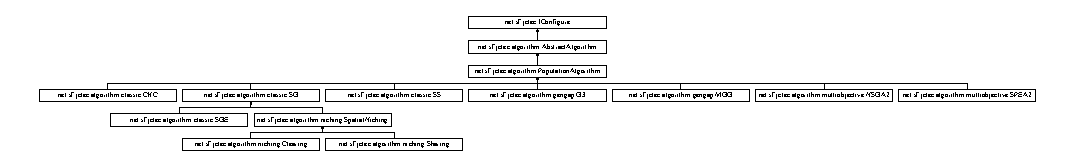
\includegraphics[height=1.797753cm]{classnet_1_1sf_1_1jclec_1_1algorithm_1_1_abstract_algorithm}
\end{center}
\end{figure}
\subsection*{Public Member Functions}
\begin{DoxyCompactItemize}
\item 
\hyperlink{classnet_1_1sf_1_1jclec_1_1algorithm_1_1_abstract_algorithm_ac2e5c4ea357824558d6c3bbb0bce0f73}{Abstract\-Algorithm} ()
\item 
final void \hyperlink{classnet_1_1sf_1_1jclec_1_1algorithm_1_1_abstract_algorithm_a3c148de7a175a933c9b2b75d93bb8983}{add\-Listener} (\hyperlink{interfacenet_1_1sf_1_1jclec_1_1_i_algorithm_listener}{I\-Algorithm\-Listener} listener)
\item 
final boolean \hyperlink{classnet_1_1sf_1_1jclec_1_1algorithm_1_1_abstract_algorithm_af18598a2578b59b0eafaf93a0fdbd0f7}{remove\-Listener} (\hyperlink{interfacenet_1_1sf_1_1jclec_1_1_i_algorithm_listener}{I\-Algorithm\-Listener} listener)
\item 
void \hyperlink{classnet_1_1sf_1_1jclec_1_1algorithm_1_1_abstract_algorithm_a0c0f69d801c64f6ebbab577916b6afe7}{pause} ()
\item 
void \hyperlink{classnet_1_1sf_1_1jclec_1_1algorithm_1_1_abstract_algorithm_a5ac6c8aaf7cba84ea5d8f2cdce3c2e35}{terminate} ()
\item 
void \hyperlink{classnet_1_1sf_1_1jclec_1_1algorithm_1_1_abstract_algorithm_a3c98847b0344873515d5c789f2989bd6}{execute} ()
\item 
void \hyperlink{classnet_1_1sf_1_1jclec_1_1algorithm_1_1_abstract_algorithm_a3322daabec936383c2cfb639b8e7b30b}{configure} (Configuration configuration)
\end{DoxyCompactItemize}
\subsection*{Protected Member Functions}
\begin{DoxyCompactItemize}
\item 
abstract void \hyperlink{classnet_1_1sf_1_1jclec_1_1algorithm_1_1_abstract_algorithm_a9cb5c0abb0c171944290260eccbc0078}{do\-Init} ()
\item 
abstract void \hyperlink{classnet_1_1sf_1_1jclec_1_1algorithm_1_1_abstract_algorithm_a09fc578d0a50e795e9ce6d0a62257f0e}{do\-Iterate} ()
\end{DoxyCompactItemize}
\subsection*{Protected Attributes}
\begin{DoxyCompactItemize}
\item 
int \hyperlink{classnet_1_1sf_1_1jclec_1_1algorithm_1_1_abstract_algorithm_a57aa821e8c2d20d94421e8464795e583}{state} = N\-E\-W
\item 
Array\-List$<$ \hyperlink{interfacenet_1_1sf_1_1jclec_1_1_i_algorithm_listener}{I\-Algorithm\-Listener} $>$ \hyperlink{classnet_1_1sf_1_1jclec_1_1algorithm_1_1_abstract_algorithm_aa03e0690e3b2883154d82ad58d59a365}{listeners} = new Array\-List$<$\hyperlink{interfacenet_1_1sf_1_1jclec_1_1_i_algorithm_listener}{I\-Algorithm\-Listener}$>$()
\end{DoxyCompactItemize}


\subsection{Detailed Description}
I\-Algorithm abstract implementation.

\begin{DoxyAuthor}{Author}
Sebastian Ventura 
\end{DoxyAuthor}


\subsection{Constructor \& Destructor Documentation}
\hypertarget{classnet_1_1sf_1_1jclec_1_1algorithm_1_1_abstract_algorithm_ac2e5c4ea357824558d6c3bbb0bce0f73}{\index{net\-::sf\-::jclec\-::algorithm\-::\-Abstract\-Algorithm@{net\-::sf\-::jclec\-::algorithm\-::\-Abstract\-Algorithm}!Abstract\-Algorithm@{Abstract\-Algorithm}}
\index{Abstract\-Algorithm@{Abstract\-Algorithm}!net::sf::jclec::algorithm::AbstractAlgorithm@{net\-::sf\-::jclec\-::algorithm\-::\-Abstract\-Algorithm}}
\subsubsection[{Abstract\-Algorithm}]{\setlength{\rightskip}{0pt plus 5cm}net.\-sf.\-jclec.\-algorithm.\-Abstract\-Algorithm.\-Abstract\-Algorithm (
\begin{DoxyParamCaption}
{}
\end{DoxyParamCaption}
)}}\label{classnet_1_1sf_1_1jclec_1_1algorithm_1_1_abstract_algorithm_ac2e5c4ea357824558d6c3bbb0bce0f73}
Empty (default) constructor 

\subsection{Member Function Documentation}
\hypertarget{classnet_1_1sf_1_1jclec_1_1algorithm_1_1_abstract_algorithm_a3c148de7a175a933c9b2b75d93bb8983}{\index{net\-::sf\-::jclec\-::algorithm\-::\-Abstract\-Algorithm@{net\-::sf\-::jclec\-::algorithm\-::\-Abstract\-Algorithm}!add\-Listener@{add\-Listener}}
\index{add\-Listener@{add\-Listener}!net::sf::jclec::algorithm::AbstractAlgorithm@{net\-::sf\-::jclec\-::algorithm\-::\-Abstract\-Algorithm}}
\subsubsection[{add\-Listener}]{\setlength{\rightskip}{0pt plus 5cm}final void net.\-sf.\-jclec.\-algorithm.\-Abstract\-Algorithm.\-add\-Listener (
\begin{DoxyParamCaption}
\item[{{\bf I\-Algorithm\-Listener}}]{listener}
\end{DoxyParamCaption}
)}}\label{classnet_1_1sf_1_1jclec_1_1algorithm_1_1_abstract_algorithm_a3c148de7a175a933c9b2b75d93bb8983}
\hypertarget{classnet_1_1sf_1_1jclec_1_1algorithm_1_1_abstract_algorithm_a3322daabec936383c2cfb639b8e7b30b}{\index{net\-::sf\-::jclec\-::algorithm\-::\-Abstract\-Algorithm@{net\-::sf\-::jclec\-::algorithm\-::\-Abstract\-Algorithm}!configure@{configure}}
\index{configure@{configure}!net::sf::jclec::algorithm::AbstractAlgorithm@{net\-::sf\-::jclec\-::algorithm\-::\-Abstract\-Algorithm}}
\subsubsection[{configure}]{\setlength{\rightskip}{0pt plus 5cm}void net.\-sf.\-jclec.\-algorithm.\-Abstract\-Algorithm.\-configure (
\begin{DoxyParamCaption}
\item[{Configuration}]{configuration}
\end{DoxyParamCaption}
)}}\label{classnet_1_1sf_1_1jclec_1_1algorithm_1_1_abstract_algorithm_a3322daabec936383c2cfb639b8e7b30b}
Configuration method.


\begin{DoxyParams}{Parameters}
{\em settings} & Configuration settings\\
\hline
\end{DoxyParams}


This method register one or several algorithm listeners to this algorithm. 

Implements \hyperlink{interfacenet_1_1sf_1_1jclec_1_1_i_configure_add31a65a04d148c690a956fbbad6987c}{net.\-sf.\-jclec.\-I\-Configure}.

\hypertarget{classnet_1_1sf_1_1jclec_1_1algorithm_1_1_abstract_algorithm_a9cb5c0abb0c171944290260eccbc0078}{\index{net\-::sf\-::jclec\-::algorithm\-::\-Abstract\-Algorithm@{net\-::sf\-::jclec\-::algorithm\-::\-Abstract\-Algorithm}!do\-Init@{do\-Init}}
\index{do\-Init@{do\-Init}!net::sf::jclec::algorithm::AbstractAlgorithm@{net\-::sf\-::jclec\-::algorithm\-::\-Abstract\-Algorithm}}
\subsubsection[{do\-Init}]{\setlength{\rightskip}{0pt plus 5cm}abstract void net.\-sf.\-jclec.\-algorithm.\-Abstract\-Algorithm.\-do\-Init (
\begin{DoxyParamCaption}
{}
\end{DoxyParamCaption}
)\hspace{0.3cm}{\ttfamily [protected]}, {\ttfamily [pure virtual]}}}\label{classnet_1_1sf_1_1jclec_1_1algorithm_1_1_abstract_algorithm_a9cb5c0abb0c171944290260eccbc0078}
Perform algorithm initialization. 

Implemented in \hyperlink{classnet_1_1sf_1_1jclec_1_1algorithm_1_1_population_algorithm_a12d1220c7c348e50a2df1abe1372b710}{net.\-sf.\-jclec.\-algorithm.\-Population\-Algorithm}, \hyperlink{classnet_1_1sf_1_1jclec_1_1algorithm_1_1classic_1_1_c_h_c_aa707ae364027caf08eba0499fc310efe}{net.\-sf.\-jclec.\-algorithm.\-classic.\-C\-H\-C}, \hyperlink{classnet_1_1sf_1_1jclec_1_1algorithm_1_1gengap_1_1_g3_aa63856d552765e073a18a74708555e18}{net.\-sf.\-jclec.\-algorithm.\-gengap.\-G3}, and \hyperlink{classnet_1_1sf_1_1jclec_1_1algorithm_1_1gengap_1_1_m_g_g_a1f3e97ac852d30a6e42f1f8a95d8b624}{net.\-sf.\-jclec.\-algorithm.\-gengap.\-M\-G\-G}.

\hypertarget{classnet_1_1sf_1_1jclec_1_1algorithm_1_1_abstract_algorithm_a09fc578d0a50e795e9ce6d0a62257f0e}{\index{net\-::sf\-::jclec\-::algorithm\-::\-Abstract\-Algorithm@{net\-::sf\-::jclec\-::algorithm\-::\-Abstract\-Algorithm}!do\-Iterate@{do\-Iterate}}
\index{do\-Iterate@{do\-Iterate}!net::sf::jclec::algorithm::AbstractAlgorithm@{net\-::sf\-::jclec\-::algorithm\-::\-Abstract\-Algorithm}}
\subsubsection[{do\-Iterate}]{\setlength{\rightskip}{0pt plus 5cm}abstract void net.\-sf.\-jclec.\-algorithm.\-Abstract\-Algorithm.\-do\-Iterate (
\begin{DoxyParamCaption}
{}
\end{DoxyParamCaption}
)\hspace{0.3cm}{\ttfamily [protected]}, {\ttfamily [pure virtual]}}}\label{classnet_1_1sf_1_1jclec_1_1algorithm_1_1_abstract_algorithm_a09fc578d0a50e795e9ce6d0a62257f0e}
Perform an algorithm iteration. 

Implemented in \hyperlink{classnet_1_1sf_1_1jclec_1_1algorithm_1_1_population_algorithm_ab5d1f94dc78fdfb100cf00d326fd59d5}{net.\-sf.\-jclec.\-algorithm.\-Population\-Algorithm}.

\hypertarget{classnet_1_1sf_1_1jclec_1_1algorithm_1_1_abstract_algorithm_a3c98847b0344873515d5c789f2989bd6}{\index{net\-::sf\-::jclec\-::algorithm\-::\-Abstract\-Algorithm@{net\-::sf\-::jclec\-::algorithm\-::\-Abstract\-Algorithm}!execute@{execute}}
\index{execute@{execute}!net::sf::jclec::algorithm::AbstractAlgorithm@{net\-::sf\-::jclec\-::algorithm\-::\-Abstract\-Algorithm}}
\subsubsection[{execute}]{\setlength{\rightskip}{0pt plus 5cm}void net.\-sf.\-jclec.\-algorithm.\-Abstract\-Algorithm.\-execute (
\begin{DoxyParamCaption}
{}
\end{DoxyParamCaption}
)}}\label{classnet_1_1sf_1_1jclec_1_1algorithm_1_1_abstract_algorithm_a3c98847b0344873515d5c789f2989bd6}
\hypertarget{classnet_1_1sf_1_1jclec_1_1algorithm_1_1_abstract_algorithm_a0c0f69d801c64f6ebbab577916b6afe7}{\index{net\-::sf\-::jclec\-::algorithm\-::\-Abstract\-Algorithm@{net\-::sf\-::jclec\-::algorithm\-::\-Abstract\-Algorithm}!pause@{pause}}
\index{pause@{pause}!net::sf::jclec::algorithm::AbstractAlgorithm@{net\-::sf\-::jclec\-::algorithm\-::\-Abstract\-Algorithm}}
\subsubsection[{pause}]{\setlength{\rightskip}{0pt plus 5cm}void net.\-sf.\-jclec.\-algorithm.\-Abstract\-Algorithm.\-pause (
\begin{DoxyParamCaption}
{}
\end{DoxyParamCaption}
)}}\label{classnet_1_1sf_1_1jclec_1_1algorithm_1_1_abstract_algorithm_a0c0f69d801c64f6ebbab577916b6afe7}
\hypertarget{classnet_1_1sf_1_1jclec_1_1algorithm_1_1_abstract_algorithm_af18598a2578b59b0eafaf93a0fdbd0f7}{\index{net\-::sf\-::jclec\-::algorithm\-::\-Abstract\-Algorithm@{net\-::sf\-::jclec\-::algorithm\-::\-Abstract\-Algorithm}!remove\-Listener@{remove\-Listener}}
\index{remove\-Listener@{remove\-Listener}!net::sf::jclec::algorithm::AbstractAlgorithm@{net\-::sf\-::jclec\-::algorithm\-::\-Abstract\-Algorithm}}
\subsubsection[{remove\-Listener}]{\setlength{\rightskip}{0pt plus 5cm}final boolean net.\-sf.\-jclec.\-algorithm.\-Abstract\-Algorithm.\-remove\-Listener (
\begin{DoxyParamCaption}
\item[{{\bf I\-Algorithm\-Listener}}]{listener}
\end{DoxyParamCaption}
)}}\label{classnet_1_1sf_1_1jclec_1_1algorithm_1_1_abstract_algorithm_af18598a2578b59b0eafaf93a0fdbd0f7}
\hypertarget{classnet_1_1sf_1_1jclec_1_1algorithm_1_1_abstract_algorithm_a5ac6c8aaf7cba84ea5d8f2cdce3c2e35}{\index{net\-::sf\-::jclec\-::algorithm\-::\-Abstract\-Algorithm@{net\-::sf\-::jclec\-::algorithm\-::\-Abstract\-Algorithm}!terminate@{terminate}}
\index{terminate@{terminate}!net::sf::jclec::algorithm::AbstractAlgorithm@{net\-::sf\-::jclec\-::algorithm\-::\-Abstract\-Algorithm}}
\subsubsection[{terminate}]{\setlength{\rightskip}{0pt plus 5cm}void net.\-sf.\-jclec.\-algorithm.\-Abstract\-Algorithm.\-terminate (
\begin{DoxyParamCaption}
{}
\end{DoxyParamCaption}
)}}\label{classnet_1_1sf_1_1jclec_1_1algorithm_1_1_abstract_algorithm_a5ac6c8aaf7cba84ea5d8f2cdce3c2e35}


\subsection{Member Data Documentation}
\hypertarget{classnet_1_1sf_1_1jclec_1_1algorithm_1_1_abstract_algorithm_aa03e0690e3b2883154d82ad58d59a365}{\index{net\-::sf\-::jclec\-::algorithm\-::\-Abstract\-Algorithm@{net\-::sf\-::jclec\-::algorithm\-::\-Abstract\-Algorithm}!listeners@{listeners}}
\index{listeners@{listeners}!net::sf::jclec::algorithm::AbstractAlgorithm@{net\-::sf\-::jclec\-::algorithm\-::\-Abstract\-Algorithm}}
\subsubsection[{listeners}]{\setlength{\rightskip}{0pt plus 5cm}Array\-List$<${\bf I\-Algorithm\-Listener}$>$ net.\-sf.\-jclec.\-algorithm.\-Abstract\-Algorithm.\-listeners = new Array\-List$<${\bf I\-Algorithm\-Listener}$>$()\hspace{0.3cm}{\ttfamily [protected]}}}\label{classnet_1_1sf_1_1jclec_1_1algorithm_1_1_abstract_algorithm_aa03e0690e3b2883154d82ad58d59a365}
Registered listeners collection \hypertarget{classnet_1_1sf_1_1jclec_1_1algorithm_1_1_abstract_algorithm_a57aa821e8c2d20d94421e8464795e583}{\index{net\-::sf\-::jclec\-::algorithm\-::\-Abstract\-Algorithm@{net\-::sf\-::jclec\-::algorithm\-::\-Abstract\-Algorithm}!state@{state}}
\index{state@{state}!net::sf::jclec::algorithm::AbstractAlgorithm@{net\-::sf\-::jclec\-::algorithm\-::\-Abstract\-Algorithm}}
\subsubsection[{state}]{\setlength{\rightskip}{0pt plus 5cm}int net.\-sf.\-jclec.\-algorithm.\-Abstract\-Algorithm.\-state = N\-E\-W\hspace{0.3cm}{\ttfamily [protected]}}}\label{classnet_1_1sf_1_1jclec_1_1algorithm_1_1_abstract_algorithm_a57aa821e8c2d20d94421e8464795e583}
Current algorithm state 

The documentation for this class was generated from the following file\-:\begin{DoxyCompactItemize}
\item 
src/main/java/net/sf/jclec/algorithm/Abstract\-Algorithm.\-java\end{DoxyCompactItemize}

\hypertarget{classnet_1_1sf_1_1jclec_1_1base_1_1_abstract_creator}{\section{net.\-sf.\-jclec.\-base.\-Abstract\-Creator Class Reference}
\label{classnet_1_1sf_1_1jclec_1_1base_1_1_abstract_creator}\index{net.\-sf.\-jclec.\-base.\-Abstract\-Creator@{net.\-sf.\-jclec.\-base.\-Abstract\-Creator}}
}
Inheritance diagram for net.\-sf.\-jclec.\-base.\-Abstract\-Creator\-:\begin{figure}[H]
\begin{center}
\leavevmode
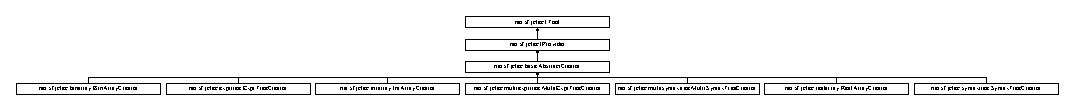
\includegraphics[height=1.042345cm]{classnet_1_1sf_1_1jclec_1_1base_1_1_abstract_creator}
\end{center}
\end{figure}
\subsection*{Public Member Functions}
\begin{DoxyCompactItemize}
\item 
\hyperlink{classnet_1_1sf_1_1jclec_1_1base_1_1_abstract_creator_a2241ce996d81607859eec1a3c9cf4767}{Abstract\-Creator} ()
\item 
void \hyperlink{classnet_1_1sf_1_1jclec_1_1base_1_1_abstract_creator_a4528e7dbcb4715766d9f877ee6257069}{contextualize} (\hyperlink{interfacenet_1_1sf_1_1jclec_1_1_i_system}{I\-System} \hyperlink{classnet_1_1sf_1_1jclec_1_1base_1_1_abstract_creator_a292f35dcb2a8428bee69e67bdfc4fe01}{context})
\item 
List$<$ \hyperlink{interfacenet_1_1sf_1_1jclec_1_1_i_individual}{I\-Individual} $>$ \hyperlink{classnet_1_1sf_1_1jclec_1_1base_1_1_abstract_creator_a96dcee22b134108056b56515c6043d9b}{provide} (int \hyperlink{classnet_1_1sf_1_1jclec_1_1base_1_1_abstract_creator_afef0fbae3aaff5c5cede8aa5e4e647ca}{number\-Of\-Individuals})
\end{DoxyCompactItemize}
\subsection*{Protected Member Functions}
\begin{DoxyCompactItemize}
\item 
abstract void \hyperlink{classnet_1_1sf_1_1jclec_1_1base_1_1_abstract_creator_a75beaef8489c52782e0c7c956c2beaf7}{prepare\-Creation} ()
\item 
abstract void \hyperlink{classnet_1_1sf_1_1jclec_1_1base_1_1_abstract_creator_aee6bcace778e7421fc5c07e1a4f6fed9}{create\-Next} ()
\end{DoxyCompactItemize}
\subsection*{Protected Attributes}
\begin{DoxyCompactItemize}
\item 
\hyperlink{interfacenet_1_1sf_1_1jclec_1_1_i_population}{I\-Population} \hyperlink{classnet_1_1sf_1_1jclec_1_1base_1_1_abstract_creator_a292f35dcb2a8428bee69e67bdfc4fe01}{context}
\item 
\hyperlink{interfacenet_1_1sf_1_1jclec_1_1util_1_1random_1_1_i_rand_gen}{I\-Rand\-Gen} \hyperlink{classnet_1_1sf_1_1jclec_1_1base_1_1_abstract_creator_a175271e8ff13e6d72d35c2daa0c75880}{randgen}
\item 
transient int \hyperlink{classnet_1_1sf_1_1jclec_1_1base_1_1_abstract_creator_afef0fbae3aaff5c5cede8aa5e4e647ca}{number\-Of\-Individuals}
\item 
transient List$<$ \hyperlink{interfacenet_1_1sf_1_1jclec_1_1_i_individual}{I\-Individual} $>$ \hyperlink{classnet_1_1sf_1_1jclec_1_1base_1_1_abstract_creator_a22720199ae989de1209e83a4df38969b}{created\-Buffer}
\item 
transient int \hyperlink{classnet_1_1sf_1_1jclec_1_1base_1_1_abstract_creator_a662f9a47a43349b37ff302a5105ca29b}{created\-Counter}
\end{DoxyCompactItemize}


\subsection{Detailed Description}
Provide new individuals creating them at random.

\begin{DoxyAuthor}{Author}
Sebastian Ventura 
\end{DoxyAuthor}


\subsection{Constructor \& Destructor Documentation}
\hypertarget{classnet_1_1sf_1_1jclec_1_1base_1_1_abstract_creator_a2241ce996d81607859eec1a3c9cf4767}{\index{net\-::sf\-::jclec\-::base\-::\-Abstract\-Creator@{net\-::sf\-::jclec\-::base\-::\-Abstract\-Creator}!Abstract\-Creator@{Abstract\-Creator}}
\index{Abstract\-Creator@{Abstract\-Creator}!net::sf::jclec::base::AbstractCreator@{net\-::sf\-::jclec\-::base\-::\-Abstract\-Creator}}
\subsubsection[{Abstract\-Creator}]{\setlength{\rightskip}{0pt plus 5cm}net.\-sf.\-jclec.\-base.\-Abstract\-Creator.\-Abstract\-Creator (
\begin{DoxyParamCaption}
{}
\end{DoxyParamCaption}
)}}\label{classnet_1_1sf_1_1jclec_1_1base_1_1_abstract_creator_a2241ce996d81607859eec1a3c9cf4767}
Empty (default) constructor. 

\subsection{Member Function Documentation}
\hypertarget{classnet_1_1sf_1_1jclec_1_1base_1_1_abstract_creator_a4528e7dbcb4715766d9f877ee6257069}{\index{net\-::sf\-::jclec\-::base\-::\-Abstract\-Creator@{net\-::sf\-::jclec\-::base\-::\-Abstract\-Creator}!contextualize@{contextualize}}
\index{contextualize@{contextualize}!net::sf::jclec::base::AbstractCreator@{net\-::sf\-::jclec\-::base\-::\-Abstract\-Creator}}
\subsubsection[{contextualize}]{\setlength{\rightskip}{0pt plus 5cm}void net.\-sf.\-jclec.\-base.\-Abstract\-Creator.\-contextualize (
\begin{DoxyParamCaption}
\item[{{\bf I\-System}}]{context}
\end{DoxyParamCaption}
)}}\label{classnet_1_1sf_1_1jclec_1_1base_1_1_abstract_creator_a4528e7dbcb4715766d9f877ee6257069}
Set the system where ...


\begin{DoxyParams}{Parameters}
{\em context} & Execution context\\
\hline
\end{DoxyParams}
 

Implements \hyperlink{interfacenet_1_1sf_1_1jclec_1_1_i_tool_aa11b3e046b7f38e40eb4f8c72a9a2102}{net.\-sf.\-jclec.\-I\-Tool}.

\hypertarget{classnet_1_1sf_1_1jclec_1_1base_1_1_abstract_creator_aee6bcace778e7421fc5c07e1a4f6fed9}{\index{net\-::sf\-::jclec\-::base\-::\-Abstract\-Creator@{net\-::sf\-::jclec\-::base\-::\-Abstract\-Creator}!create\-Next@{create\-Next}}
\index{create\-Next@{create\-Next}!net::sf::jclec::base::AbstractCreator@{net\-::sf\-::jclec\-::base\-::\-Abstract\-Creator}}
\subsubsection[{create\-Next}]{\setlength{\rightskip}{0pt plus 5cm}abstract void net.\-sf.\-jclec.\-base.\-Abstract\-Creator.\-create\-Next (
\begin{DoxyParamCaption}
{}
\end{DoxyParamCaption}
)\hspace{0.3cm}{\ttfamily [protected]}, {\ttfamily [pure virtual]}}}\label{classnet_1_1sf_1_1jclec_1_1base_1_1_abstract_creator_aee6bcace778e7421fc5c07e1a4f6fed9}
Creation method.


\begin{DoxyParams}{Parameters}
{\em ind} & Individual to create\\
\hline
\end{DoxyParams}
\begin{DoxyReturn}{Returns}
New individual 
\end{DoxyReturn}


Implemented in \hyperlink{classnet_1_1sf_1_1jclec_1_1binarray_1_1_bin_array_creator_aff93b467bf15009d84d97e5427398985}{net.\-sf.\-jclec.\-binarray.\-Bin\-Array\-Creator}, \hyperlink{classnet_1_1sf_1_1jclec_1_1multiexprtree_1_1_multi_expr_tree_creator_a09d421b3322dd569eed75df1785d070b}{net.\-sf.\-jclec.\-multiexprtree.\-Multi\-Expr\-Tree\-Creator}, \hyperlink{classnet_1_1sf_1_1jclec_1_1exprtree_1_1_expr_tree_creator_afbb105f831c250f0ec1309536359bd63}{net.\-sf.\-jclec.\-exprtree.\-Expr\-Tree\-Creator}, \hyperlink{classnet_1_1sf_1_1jclec_1_1multisyntaxtree_1_1_multi_syntax_tree_creator_a33223297fd1f40f4ef10bd1b1ec31a5a}{net.\-sf.\-jclec.\-multisyntaxtree.\-Multi\-Syntax\-Tree\-Creator}, \hyperlink{classnet_1_1sf_1_1jclec_1_1realarray_1_1_real_array_creator_a4c4d021fbc4923f45748f67f66d3b59d}{net.\-sf.\-jclec.\-realarray.\-Real\-Array\-Creator}, \hyperlink{classnet_1_1sf_1_1jclec_1_1intarray_1_1_int_array_creator_a099e0903120e3f6ed37eacaf79be97ca}{net.\-sf.\-jclec.\-intarray.\-Int\-Array\-Creator}, and \hyperlink{classnet_1_1sf_1_1jclec_1_1syntaxtree_1_1_syntax_tree_creator_a53ed3752c93350b456ff5cdc1b4bfbe8}{net.\-sf.\-jclec.\-syntaxtree.\-Syntax\-Tree\-Creator}.

\hypertarget{classnet_1_1sf_1_1jclec_1_1base_1_1_abstract_creator_a75beaef8489c52782e0c7c956c2beaf7}{\index{net\-::sf\-::jclec\-::base\-::\-Abstract\-Creator@{net\-::sf\-::jclec\-::base\-::\-Abstract\-Creator}!prepare\-Creation@{prepare\-Creation}}
\index{prepare\-Creation@{prepare\-Creation}!net::sf::jclec::base::AbstractCreator@{net\-::sf\-::jclec\-::base\-::\-Abstract\-Creator}}
\subsubsection[{prepare\-Creation}]{\setlength{\rightskip}{0pt plus 5cm}abstract void net.\-sf.\-jclec.\-base.\-Abstract\-Creator.\-prepare\-Creation (
\begin{DoxyParamCaption}
{}
\end{DoxyParamCaption}
)\hspace{0.3cm}{\ttfamily [protected]}, {\ttfamily [pure virtual]}}}\label{classnet_1_1sf_1_1jclec_1_1base_1_1_abstract_creator_a75beaef8489c52782e0c7c956c2beaf7}
Prepare creation process. 

Implemented in \hyperlink{classnet_1_1sf_1_1jclec_1_1multiexprtree_1_1_multi_expr_tree_creator_a6f478c0740a3c7f2452786a913e733a0}{net.\-sf.\-jclec.\-multiexprtree.\-Multi\-Expr\-Tree\-Creator}, \hyperlink{classnet_1_1sf_1_1jclec_1_1exprtree_1_1_expr_tree_creator_a00264d7b01aa199cc1263302a503e378}{net.\-sf.\-jclec.\-exprtree.\-Expr\-Tree\-Creator}, \hyperlink{classnet_1_1sf_1_1jclec_1_1binarray_1_1_bin_array_creator_a51d110d716e41756a37c508a5d92b478}{net.\-sf.\-jclec.\-binarray.\-Bin\-Array\-Creator}, \hyperlink{classnet_1_1sf_1_1jclec_1_1multisyntaxtree_1_1_multi_syntax_tree_creator_a06e967d582acf36dc8dc39959c55e6c3}{net.\-sf.\-jclec.\-multisyntaxtree.\-Multi\-Syntax\-Tree\-Creator}, \hyperlink{classnet_1_1sf_1_1jclec_1_1realarray_1_1_real_array_creator_a60cd5c3f11c12bca77893b6b1cb665af}{net.\-sf.\-jclec.\-realarray.\-Real\-Array\-Creator}, \hyperlink{classnet_1_1sf_1_1jclec_1_1intarray_1_1_int_array_creator_a84dde310784a8ef9935e82195b963136}{net.\-sf.\-jclec.\-intarray.\-Int\-Array\-Creator}, and \hyperlink{classnet_1_1sf_1_1jclec_1_1syntaxtree_1_1_syntax_tree_creator_adf7abfdb8c0667909f2c751f5ea3c36e}{net.\-sf.\-jclec.\-syntaxtree.\-Syntax\-Tree\-Creator}.

\hypertarget{classnet_1_1sf_1_1jclec_1_1base_1_1_abstract_creator_a96dcee22b134108056b56515c6043d9b}{\index{net\-::sf\-::jclec\-::base\-::\-Abstract\-Creator@{net\-::sf\-::jclec\-::base\-::\-Abstract\-Creator}!provide@{provide}}
\index{provide@{provide}!net::sf::jclec::base::AbstractCreator@{net\-::sf\-::jclec\-::base\-::\-Abstract\-Creator}}
\subsubsection[{provide}]{\setlength{\rightskip}{0pt plus 5cm}List$<${\bf I\-Individual}$>$ net.\-sf.\-jclec.\-base.\-Abstract\-Creator.\-provide (
\begin{DoxyParamCaption}
\item[{int}]{number\-Of\-Individuals}
\end{DoxyParamCaption}
)}}\label{classnet_1_1sf_1_1jclec_1_1base_1_1_abstract_creator_a96dcee22b134108056b56515c6043d9b}
This method performs the following actions\-:


\begin{DoxyEnumerate}
\item Assigns the {\ttfamily number\-Of\-Individuals} parameter to the auxiliary class variable {\ttfamily this.\-number\-Of\-Individuals}  
\item Assigns a new list of {\ttfamily \hyperlink{interfacenet_1_1sf_1_1jclec_1_1_i_individual}{I\-Individual}} objects to the auxiliary class variable {\ttfamily created\-Buffer}.  
\item Call the method {\ttfamily prepare\-Creation}, that prepares the individuals creation process.  
\item Call the method {\ttfamily create\-Next} until {\ttfamily created\-Counter} is equals to {\ttfamily number\-Of\-Individuals}  
\item Return {\ttfamily created\-Buffer}.  
\end{DoxyEnumerate}

Provision method.


\begin{DoxyParams}{Parameters}
{\em number\-Of\-Individuals} & Number of individuals to provide\\
\hline
\end{DoxyParams}
\begin{DoxyReturn}{Returns}
List of provided individuals
\end{DoxyReturn}
 

Implements \hyperlink{interfacenet_1_1sf_1_1jclec_1_1_i_provider_a4e3b8fff3419d3c9f1902e26de309640}{net.\-sf.\-jclec.\-I\-Provider}.



\subsection{Member Data Documentation}
\hypertarget{classnet_1_1sf_1_1jclec_1_1base_1_1_abstract_creator_a292f35dcb2a8428bee69e67bdfc4fe01}{\index{net\-::sf\-::jclec\-::base\-::\-Abstract\-Creator@{net\-::sf\-::jclec\-::base\-::\-Abstract\-Creator}!context@{context}}
\index{context@{context}!net::sf::jclec::base::AbstractCreator@{net\-::sf\-::jclec\-::base\-::\-Abstract\-Creator}}
\subsubsection[{context}]{\setlength{\rightskip}{0pt plus 5cm}{\bf I\-Population} net.\-sf.\-jclec.\-base.\-Abstract\-Creator.\-context\hspace{0.3cm}{\ttfamily [protected]}}}\label{classnet_1_1sf_1_1jclec_1_1base_1_1_abstract_creator_a292f35dcb2a8428bee69e67bdfc4fe01}
Execution context \hypertarget{classnet_1_1sf_1_1jclec_1_1base_1_1_abstract_creator_a22720199ae989de1209e83a4df38969b}{\index{net\-::sf\-::jclec\-::base\-::\-Abstract\-Creator@{net\-::sf\-::jclec\-::base\-::\-Abstract\-Creator}!created\-Buffer@{created\-Buffer}}
\index{created\-Buffer@{created\-Buffer}!net::sf::jclec::base::AbstractCreator@{net\-::sf\-::jclec\-::base\-::\-Abstract\-Creator}}
\subsubsection[{created\-Buffer}]{\setlength{\rightskip}{0pt plus 5cm}transient List$<${\bf I\-Individual}$>$ net.\-sf.\-jclec.\-base.\-Abstract\-Creator.\-created\-Buffer\hspace{0.3cm}{\ttfamily [protected]}}}\label{classnet_1_1sf_1_1jclec_1_1base_1_1_abstract_creator_a22720199ae989de1209e83a4df38969b}
Creation buffer \hypertarget{classnet_1_1sf_1_1jclec_1_1base_1_1_abstract_creator_a662f9a47a43349b37ff302a5105ca29b}{\index{net\-::sf\-::jclec\-::base\-::\-Abstract\-Creator@{net\-::sf\-::jclec\-::base\-::\-Abstract\-Creator}!created\-Counter@{created\-Counter}}
\index{created\-Counter@{created\-Counter}!net::sf::jclec::base::AbstractCreator@{net\-::sf\-::jclec\-::base\-::\-Abstract\-Creator}}
\subsubsection[{created\-Counter}]{\setlength{\rightskip}{0pt plus 5cm}transient int net.\-sf.\-jclec.\-base.\-Abstract\-Creator.\-created\-Counter\hspace{0.3cm}{\ttfamily [protected]}}}\label{classnet_1_1sf_1_1jclec_1_1base_1_1_abstract_creator_a662f9a47a43349b37ff302a5105ca29b}
Created counter \hypertarget{classnet_1_1sf_1_1jclec_1_1base_1_1_abstract_creator_afef0fbae3aaff5c5cede8aa5e4e647ca}{\index{net\-::sf\-::jclec\-::base\-::\-Abstract\-Creator@{net\-::sf\-::jclec\-::base\-::\-Abstract\-Creator}!number\-Of\-Individuals@{number\-Of\-Individuals}}
\index{number\-Of\-Individuals@{number\-Of\-Individuals}!net::sf::jclec::base::AbstractCreator@{net\-::sf\-::jclec\-::base\-::\-Abstract\-Creator}}
\subsubsection[{number\-Of\-Individuals}]{\setlength{\rightskip}{0pt plus 5cm}transient int net.\-sf.\-jclec.\-base.\-Abstract\-Creator.\-number\-Of\-Individuals\hspace{0.3cm}{\ttfamily [protected]}}}\label{classnet_1_1sf_1_1jclec_1_1base_1_1_abstract_creator_afef0fbae3aaff5c5cede8aa5e4e647ca}
Number of individuals to create \hypertarget{classnet_1_1sf_1_1jclec_1_1base_1_1_abstract_creator_a175271e8ff13e6d72d35c2daa0c75880}{\index{net\-::sf\-::jclec\-::base\-::\-Abstract\-Creator@{net\-::sf\-::jclec\-::base\-::\-Abstract\-Creator}!randgen@{randgen}}
\index{randgen@{randgen}!net::sf::jclec::base::AbstractCreator@{net\-::sf\-::jclec\-::base\-::\-Abstract\-Creator}}
\subsubsection[{randgen}]{\setlength{\rightskip}{0pt plus 5cm}{\bf I\-Rand\-Gen} net.\-sf.\-jclec.\-base.\-Abstract\-Creator.\-randgen\hspace{0.3cm}{\ttfamily [protected]}}}\label{classnet_1_1sf_1_1jclec_1_1base_1_1_abstract_creator_a175271e8ff13e6d72d35c2daa0c75880}
Random generator used in creation 

The documentation for this class was generated from the following file\-:\begin{DoxyCompactItemize}
\item 
src/main/java/net/sf/jclec/base/Abstract\-Creator.\-java\end{DoxyCompactItemize}

\hypertarget{classnet_1_1sf_1_1jclec_1_1base_1_1_abstract_evaluator}{\section{net.\-sf.\-jclec.\-base.\-Abstract\-Evaluator Class Reference}
\label{classnet_1_1sf_1_1jclec_1_1base_1_1_abstract_evaluator}\index{net.\-sf.\-jclec.\-base.\-Abstract\-Evaluator@{net.\-sf.\-jclec.\-base.\-Abstract\-Evaluator}}
}
Inheritance diagram for net.\-sf.\-jclec.\-base.\-Abstract\-Evaluator\-:\begin{figure}[H]
\begin{center}
\leavevmode
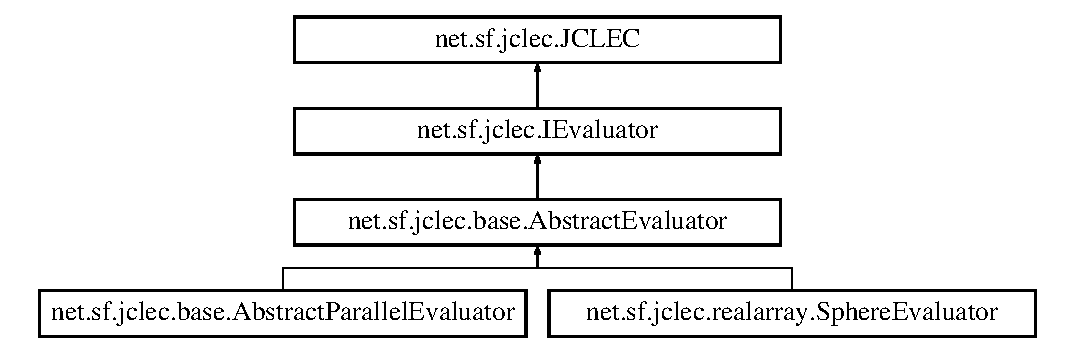
\includegraphics[height=4.000000cm]{classnet_1_1sf_1_1jclec_1_1base_1_1_abstract_evaluator}
\end{center}
\end{figure}
\subsection*{Public Member Functions}
\begin{DoxyCompactItemize}
\item 
\hyperlink{classnet_1_1sf_1_1jclec_1_1base_1_1_abstract_evaluator_a3f8105ac25e482fec118d58aa6bd9db6}{Abstract\-Evaluator} ()
\item 
int \hyperlink{classnet_1_1sf_1_1jclec_1_1base_1_1_abstract_evaluator_a4bf8163d0769193b1d92327d29cf3247}{get\-Number\-Of\-Evaluations} ()
\item 
void \hyperlink{classnet_1_1sf_1_1jclec_1_1base_1_1_abstract_evaluator_a33398832b681b02d99b739c51fef4acb}{evaluate} (List$<$ \hyperlink{interfacenet_1_1sf_1_1jclec_1_1_i_individual}{I\-Individual} $>$ inds)
\end{DoxyCompactItemize}
\subsection*{Protected Member Functions}
\begin{DoxyCompactItemize}
\item 
abstract void \hyperlink{classnet_1_1sf_1_1jclec_1_1base_1_1_abstract_evaluator_ab268ad679c75a9612d262cc957976471}{evaluate} (\hyperlink{interfacenet_1_1sf_1_1jclec_1_1_i_individual}{I\-Individual} ind)
\end{DoxyCompactItemize}


\subsection{Detailed Description}
\hyperlink{interfacenet_1_1sf_1_1jclec_1_1_i_evaluator}{I\-Evaluator} abstract implementation.

\begin{DoxyAuthor}{Author}
Sebastian Ventura 
\end{DoxyAuthor}


\subsection{Constructor \& Destructor Documentation}
\hypertarget{classnet_1_1sf_1_1jclec_1_1base_1_1_abstract_evaluator_a3f8105ac25e482fec118d58aa6bd9db6}{\index{net\-::sf\-::jclec\-::base\-::\-Abstract\-Evaluator@{net\-::sf\-::jclec\-::base\-::\-Abstract\-Evaluator}!Abstract\-Evaluator@{Abstract\-Evaluator}}
\index{Abstract\-Evaluator@{Abstract\-Evaluator}!net::sf::jclec::base::AbstractEvaluator@{net\-::sf\-::jclec\-::base\-::\-Abstract\-Evaluator}}
\subsubsection[{Abstract\-Evaluator}]{\setlength{\rightskip}{0pt plus 5cm}net.\-sf.\-jclec.\-base.\-Abstract\-Evaluator.\-Abstract\-Evaluator (
\begin{DoxyParamCaption}
{}
\end{DoxyParamCaption}
)}}\label{classnet_1_1sf_1_1jclec_1_1base_1_1_abstract_evaluator_a3f8105ac25e482fec118d58aa6bd9db6}
Empty constructor. 

\subsection{Member Function Documentation}
\hypertarget{classnet_1_1sf_1_1jclec_1_1base_1_1_abstract_evaluator_a33398832b681b02d99b739c51fef4acb}{\index{net\-::sf\-::jclec\-::base\-::\-Abstract\-Evaluator@{net\-::sf\-::jclec\-::base\-::\-Abstract\-Evaluator}!evaluate@{evaluate}}
\index{evaluate@{evaluate}!net::sf::jclec::base::AbstractEvaluator@{net\-::sf\-::jclec\-::base\-::\-Abstract\-Evaluator}}
\subsubsection[{evaluate}]{\setlength{\rightskip}{0pt plus 5cm}void net.\-sf.\-jclec.\-base.\-Abstract\-Evaluator.\-evaluate (
\begin{DoxyParamCaption}
\item[{List$<$ {\bf I\-Individual} $>$}]{inds}
\end{DoxyParamCaption}
)}}\label{classnet_1_1sf_1_1jclec_1_1base_1_1_abstract_evaluator_a33398832b681b02d99b739c51fef4acb}
For all individuals in \char`\"{}inds\char`\"{} array\-: if individual fitness is null, then evaluate this individual.

This method is final. Is anyone wants implement this method in another way should create a new \hyperlink{interfacenet_1_1sf_1_1jclec_1_1_i_evaluator}{I\-Evaluator} class.

Evaluation method.


\begin{DoxyParams}{Parameters}
{\em inds} & Individuals to evaluate\\
\hline
\end{DoxyParams}
 

Implements \hyperlink{interfacenet_1_1sf_1_1jclec_1_1_i_evaluator_a6a64b0d69f99da5be8a6c5b01c7752c2}{net.\-sf.\-jclec.\-I\-Evaluator}.

\hypertarget{classnet_1_1sf_1_1jclec_1_1base_1_1_abstract_evaluator_ab268ad679c75a9612d262cc957976471}{\index{net\-::sf\-::jclec\-::base\-::\-Abstract\-Evaluator@{net\-::sf\-::jclec\-::base\-::\-Abstract\-Evaluator}!evaluate@{evaluate}}
\index{evaluate@{evaluate}!net::sf::jclec::base::AbstractEvaluator@{net\-::sf\-::jclec\-::base\-::\-Abstract\-Evaluator}}
\subsubsection[{evaluate}]{\setlength{\rightskip}{0pt plus 5cm}abstract void net.\-sf.\-jclec.\-base.\-Abstract\-Evaluator.\-evaluate (
\begin{DoxyParamCaption}
\item[{{\bf I\-Individual}}]{ind}
\end{DoxyParamCaption}
)\hspace{0.3cm}{\ttfamily [protected]}, {\ttfamily [pure virtual]}}}\label{classnet_1_1sf_1_1jclec_1_1base_1_1_abstract_evaluator_ab268ad679c75a9612d262cc957976471}
Individual evaluation method.


\begin{DoxyParams}{Parameters}
{\em ind} & Individual to evaluate \\
\hline
\end{DoxyParams}


Implemented in \hyperlink{classnet_1_1sf_1_1jclec_1_1realarray_1_1_sphere_evaluator_a89540f711cf70d68b5c30f798e90d5fa}{net.\-sf.\-jclec.\-realarray.\-Sphere\-Evaluator}.

\hypertarget{classnet_1_1sf_1_1jclec_1_1base_1_1_abstract_evaluator_a4bf8163d0769193b1d92327d29cf3247}{\index{net\-::sf\-::jclec\-::base\-::\-Abstract\-Evaluator@{net\-::sf\-::jclec\-::base\-::\-Abstract\-Evaluator}!get\-Number\-Of\-Evaluations@{get\-Number\-Of\-Evaluations}}
\index{get\-Number\-Of\-Evaluations@{get\-Number\-Of\-Evaluations}!net::sf::jclec::base::AbstractEvaluator@{net\-::sf\-::jclec\-::base\-::\-Abstract\-Evaluator}}
\subsubsection[{get\-Number\-Of\-Evaluations}]{\setlength{\rightskip}{0pt plus 5cm}int net.\-sf.\-jclec.\-base.\-Abstract\-Evaluator.\-get\-Number\-Of\-Evaluations (
\begin{DoxyParamCaption}
{}
\end{DoxyParamCaption}
)}}\label{classnet_1_1sf_1_1jclec_1_1base_1_1_abstract_evaluator_a4bf8163d0769193b1d92327d29cf3247}
Get the number of individuals evaluated until now.

\begin{DoxyReturn}{Returns}
Number of evaluations until now
\end{DoxyReturn}
 

Implements \hyperlink{interfacenet_1_1sf_1_1jclec_1_1_i_evaluator_a16f44ac81b7f59147da746461ab66f1c}{net.\-sf.\-jclec.\-I\-Evaluator}.



The documentation for this class was generated from the following file\-:\begin{DoxyCompactItemize}
\item 
src/main/java/net/sf/jclec/base/Abstract\-Evaluator.\-java\end{DoxyCompactItemize}

\hypertarget{classnet_1_1sf_1_1jclec_1_1base_1_1_abstract_fitness}{\section{net.\-sf.\-jclec.\-base.\-Abstract\-Fitness Class Reference}
\label{classnet_1_1sf_1_1jclec_1_1base_1_1_abstract_fitness}\index{net.\-sf.\-jclec.\-base.\-Abstract\-Fitness@{net.\-sf.\-jclec.\-base.\-Abstract\-Fitness}}
}
Inheritance diagram for net.\-sf.\-jclec.\-base.\-Abstract\-Fitness\-:\begin{figure}[H]
\begin{center}
\leavevmode
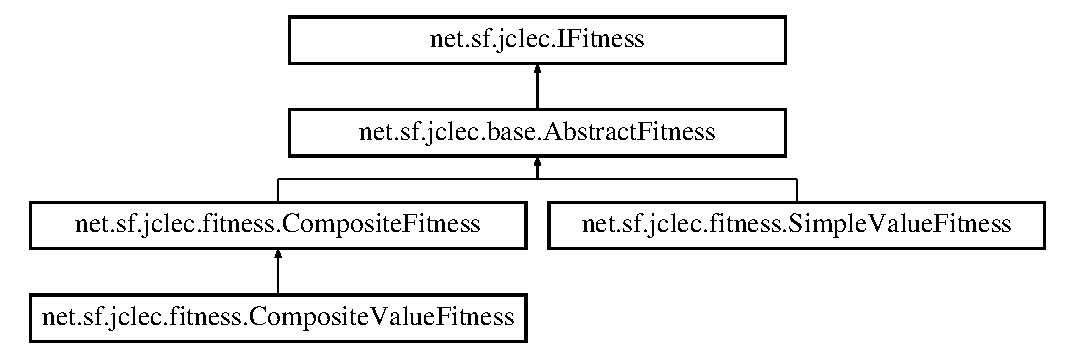
\includegraphics[height=5.000000cm]{classnet_1_1sf_1_1jclec_1_1base_1_1_abstract_fitness}
\end{center}
\end{figure}
\subsection*{Public Member Functions}
\begin{DoxyCompactItemize}
\item 
\hyperlink{classnet_1_1sf_1_1jclec_1_1base_1_1_abstract_fitness_ae2db3ac5d5a13598e00280db8f6d9ba6}{Abstract\-Fitness} ()
\item 
boolean \hyperlink{classnet_1_1sf_1_1jclec_1_1base_1_1_abstract_fitness_a7671261b00c8251f7e32f58b606c5dbc}{is\-Acceptable} ()
\end{DoxyCompactItemize}


\subsection{Detailed Description}
\hyperlink{interfacenet_1_1sf_1_1jclec_1_1_i_fitness}{I\-Fitness} abstract implementation.

\begin{DoxyAuthor}{Author}
Sebastian Ventura 
\end{DoxyAuthor}


\subsection{Constructor \& Destructor Documentation}
\hypertarget{classnet_1_1sf_1_1jclec_1_1base_1_1_abstract_fitness_ae2db3ac5d5a13598e00280db8f6d9ba6}{\index{net\-::sf\-::jclec\-::base\-::\-Abstract\-Fitness@{net\-::sf\-::jclec\-::base\-::\-Abstract\-Fitness}!Abstract\-Fitness@{Abstract\-Fitness}}
\index{Abstract\-Fitness@{Abstract\-Fitness}!net::sf::jclec::base::AbstractFitness@{net\-::sf\-::jclec\-::base\-::\-Abstract\-Fitness}}
\subsubsection[{Abstract\-Fitness}]{\setlength{\rightskip}{0pt plus 5cm}net.\-sf.\-jclec.\-base.\-Abstract\-Fitness.\-Abstract\-Fitness (
\begin{DoxyParamCaption}
{}
\end{DoxyParamCaption}
)}}\label{classnet_1_1sf_1_1jclec_1_1base_1_1_abstract_fitness_ae2db3ac5d5a13598e00280db8f6d9ba6}
Empty constructor 

\subsection{Member Function Documentation}
\hypertarget{classnet_1_1sf_1_1jclec_1_1base_1_1_abstract_fitness_a7671261b00c8251f7e32f58b606c5dbc}{\index{net\-::sf\-::jclec\-::base\-::\-Abstract\-Fitness@{net\-::sf\-::jclec\-::base\-::\-Abstract\-Fitness}!is\-Acceptable@{is\-Acceptable}}
\index{is\-Acceptable@{is\-Acceptable}!net::sf::jclec::base::AbstractFitness@{net\-::sf\-::jclec\-::base\-::\-Abstract\-Fitness}}
\subsubsection[{is\-Acceptable}]{\setlength{\rightskip}{0pt plus 5cm}boolean net.\-sf.\-jclec.\-base.\-Abstract\-Fitness.\-is\-Acceptable (
\begin{DoxyParamCaption}
{}
\end{DoxyParamCaption}
)}}\label{classnet_1_1sf_1_1jclec_1_1base_1_1_abstract_fitness_a7671261b00c8251f7e32f58b606c5dbc}
This default implementation returns false everytime.

\begin{DoxyReturn}{Returns}
false 
\end{DoxyReturn}


Implements \hyperlink{interfacenet_1_1sf_1_1jclec_1_1_i_fitness_ad71279ddab337f1624c6d767ece9cb7e}{net.\-sf.\-jclec.\-I\-Fitness}.



The documentation for this class was generated from the following file\-:\begin{DoxyCompactItemize}
\item 
src/main/java/net/sf/jclec/base/Abstract\-Fitness.\-java\end{DoxyCompactItemize}

\hypertarget{classnet_1_1sf_1_1jclec_1_1realarray_1_1rec_1_1_abstract_fuzzy_connectives}{\section{net.\-sf.\-jclec.\-realarray.\-rec.\-Abstract\-Fuzzy\-Connectives Class Reference}
\label{classnet_1_1sf_1_1jclec_1_1realarray_1_1rec_1_1_abstract_fuzzy_connectives}\index{net.\-sf.\-jclec.\-realarray.\-rec.\-Abstract\-Fuzzy\-Connectives@{net.\-sf.\-jclec.\-realarray.\-rec.\-Abstract\-Fuzzy\-Connectives}}
}
Inheritance diagram for net.\-sf.\-jclec.\-realarray.\-rec.\-Abstract\-Fuzzy\-Connectives\-:\begin{figure}[H]
\begin{center}
\leavevmode
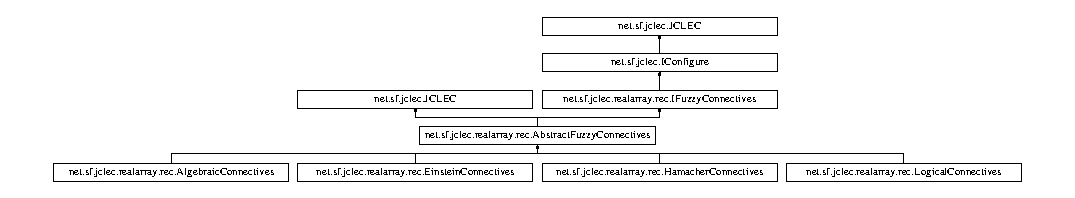
\includegraphics[height=1.766562cm]{classnet_1_1sf_1_1jclec_1_1realarray_1_1rec_1_1_abstract_fuzzy_connectives}
\end{center}
\end{figure}
\subsection*{Public Member Functions}
\begin{DoxyCompactItemize}
\item 
\hyperlink{classnet_1_1sf_1_1jclec_1_1realarray_1_1rec_1_1_abstract_fuzzy_connectives_ad4297b3bf30901127009d31637bfae1f}{Abstract\-Fuzzy\-Connectives} ()
\item 
double \hyperlink{classnet_1_1sf_1_1jclec_1_1realarray_1_1rec_1_1_abstract_fuzzy_connectives_aff5d878d9ceec7f839468d1cb716dfec}{get\-Alpha} ()
\item 
void \hyperlink{classnet_1_1sf_1_1jclec_1_1realarray_1_1rec_1_1_abstract_fuzzy_connectives_a45e699498fb9c6009e8ea066837862cc}{set\-Alpha} (double alpha)
\item 
void \hyperlink{classnet_1_1sf_1_1jclec_1_1realarray_1_1rec_1_1_abstract_fuzzy_connectives_a35538e69d56a5f2f01bdb8d485551165}{configure} (Configuration settings)
\end{DoxyCompactItemize}


\subsection{Detailed Description}
Connectives abstract implementation

\begin{DoxyAuthor}{Author}
Alberto Lamarca-\/\-Rosales 

Sebastian Ventura 
\end{DoxyAuthor}


\subsection{Constructor \& Destructor Documentation}
\hypertarget{classnet_1_1sf_1_1jclec_1_1realarray_1_1rec_1_1_abstract_fuzzy_connectives_ad4297b3bf30901127009d31637bfae1f}{\index{net\-::sf\-::jclec\-::realarray\-::rec\-::\-Abstract\-Fuzzy\-Connectives@{net\-::sf\-::jclec\-::realarray\-::rec\-::\-Abstract\-Fuzzy\-Connectives}!Abstract\-Fuzzy\-Connectives@{Abstract\-Fuzzy\-Connectives}}
\index{Abstract\-Fuzzy\-Connectives@{Abstract\-Fuzzy\-Connectives}!net::sf::jclec::realarray::rec::AbstractFuzzyConnectives@{net\-::sf\-::jclec\-::realarray\-::rec\-::\-Abstract\-Fuzzy\-Connectives}}
\subsubsection[{Abstract\-Fuzzy\-Connectives}]{\setlength{\rightskip}{0pt plus 5cm}net.\-sf.\-jclec.\-realarray.\-rec.\-Abstract\-Fuzzy\-Connectives.\-Abstract\-Fuzzy\-Connectives (
\begin{DoxyParamCaption}
{}
\end{DoxyParamCaption}
)}}\label{classnet_1_1sf_1_1jclec_1_1realarray_1_1rec_1_1_abstract_fuzzy_connectives_ad4297b3bf30901127009d31637bfae1f}
Empty constructor 

\subsection{Member Function Documentation}
\hypertarget{classnet_1_1sf_1_1jclec_1_1realarray_1_1rec_1_1_abstract_fuzzy_connectives_a35538e69d56a5f2f01bdb8d485551165}{\index{net\-::sf\-::jclec\-::realarray\-::rec\-::\-Abstract\-Fuzzy\-Connectives@{net\-::sf\-::jclec\-::realarray\-::rec\-::\-Abstract\-Fuzzy\-Connectives}!configure@{configure}}
\index{configure@{configure}!net::sf::jclec::realarray::rec::AbstractFuzzyConnectives@{net\-::sf\-::jclec\-::realarray\-::rec\-::\-Abstract\-Fuzzy\-Connectives}}
\subsubsection[{configure}]{\setlength{\rightskip}{0pt plus 5cm}void net.\-sf.\-jclec.\-realarray.\-rec.\-Abstract\-Fuzzy\-Connectives.\-configure (
\begin{DoxyParamCaption}
\item[{Configuration}]{settings}
\end{DoxyParamCaption}
)}}\label{classnet_1_1sf_1_1jclec_1_1realarray_1_1rec_1_1_abstract_fuzzy_connectives_a35538e69d56a5f2f01bdb8d485551165}
Configuration method.


\begin{DoxyParams}{Parameters}
{\em settings} & Configuration settings \\
\hline
\end{DoxyParams}


Implements \hyperlink{interfacenet_1_1sf_1_1jclec_1_1_i_configure_add31a65a04d148c690a956fbbad6987c}{net.\-sf.\-jclec.\-I\-Configure}.

\hypertarget{classnet_1_1sf_1_1jclec_1_1realarray_1_1rec_1_1_abstract_fuzzy_connectives_aff5d878d9ceec7f839468d1cb716dfec}{\index{net\-::sf\-::jclec\-::realarray\-::rec\-::\-Abstract\-Fuzzy\-Connectives@{net\-::sf\-::jclec\-::realarray\-::rec\-::\-Abstract\-Fuzzy\-Connectives}!get\-Alpha@{get\-Alpha}}
\index{get\-Alpha@{get\-Alpha}!net::sf::jclec::realarray::rec::AbstractFuzzyConnectives@{net\-::sf\-::jclec\-::realarray\-::rec\-::\-Abstract\-Fuzzy\-Connectives}}
\subsubsection[{get\-Alpha}]{\setlength{\rightskip}{0pt plus 5cm}double net.\-sf.\-jclec.\-realarray.\-rec.\-Abstract\-Fuzzy\-Connectives.\-get\-Alpha (
\begin{DoxyParamCaption}
{}
\end{DoxyParamCaption}
)}}\label{classnet_1_1sf_1_1jclec_1_1realarray_1_1rec_1_1_abstract_fuzzy_connectives_aff5d878d9ceec7f839468d1cb716dfec}
\begin{DoxyReturn}{Returns}
Actual alpha value 
\end{DoxyReturn}


Implements \hyperlink{interfacenet_1_1sf_1_1jclec_1_1realarray_1_1rec_1_1_i_fuzzy_connectives_a307541244373dc0e116dc64452b1e354}{net.\-sf.\-jclec.\-realarray.\-rec.\-I\-Fuzzy\-Connectives}.

\hypertarget{classnet_1_1sf_1_1jclec_1_1realarray_1_1rec_1_1_abstract_fuzzy_connectives_a45e699498fb9c6009e8ea066837862cc}{\index{net\-::sf\-::jclec\-::realarray\-::rec\-::\-Abstract\-Fuzzy\-Connectives@{net\-::sf\-::jclec\-::realarray\-::rec\-::\-Abstract\-Fuzzy\-Connectives}!set\-Alpha@{set\-Alpha}}
\index{set\-Alpha@{set\-Alpha}!net::sf::jclec::realarray::rec::AbstractFuzzyConnectives@{net\-::sf\-::jclec\-::realarray\-::rec\-::\-Abstract\-Fuzzy\-Connectives}}
\subsubsection[{set\-Alpha}]{\setlength{\rightskip}{0pt plus 5cm}void net.\-sf.\-jclec.\-realarray.\-rec.\-Abstract\-Fuzzy\-Connectives.\-set\-Alpha (
\begin{DoxyParamCaption}
\item[{double}]{alpha}
\end{DoxyParamCaption}
)}}\label{classnet_1_1sf_1_1jclec_1_1realarray_1_1rec_1_1_abstract_fuzzy_connectives_a45e699498fb9c6009e8ea066837862cc}
Sets the alpha value, used in ...


\begin{DoxyParams}{Parameters}
{\em alpha} & New alpha value \\
\hline
\end{DoxyParams}


Implements \hyperlink{interfacenet_1_1sf_1_1jclec_1_1realarray_1_1rec_1_1_i_fuzzy_connectives_a33e828ad2d1f45c8485c7cc1c9512949}{net.\-sf.\-jclec.\-realarray.\-rec.\-I\-Fuzzy\-Connectives}.



The documentation for this class was generated from the following file\-:\begin{DoxyCompactItemize}
\item 
src/main/java/net/sf/jclec/realarray/rec/Abstract\-Fuzzy\-Connectives.\-java\end{DoxyCompactItemize}

\hypertarget{classnet_1_1sf_1_1jclec_1_1base_1_1_abstract_individual_3_01_g_01_4}{\section{net.\-sf.\-jclec.\-base.\-Abstract\-Individual$<$ G $>$ Class Reference}
\label{classnet_1_1sf_1_1jclec_1_1base_1_1_abstract_individual_3_01_g_01_4}\index{net.\-sf.\-jclec.\-base.\-Abstract\-Individual$<$ G $>$@{net.\-sf.\-jclec.\-base.\-Abstract\-Individual$<$ G $>$}}
}
Inheritance diagram for net.\-sf.\-jclec.\-base.\-Abstract\-Individual$<$ G $>$\-:\begin{figure}[H]
\begin{center}
\leavevmode
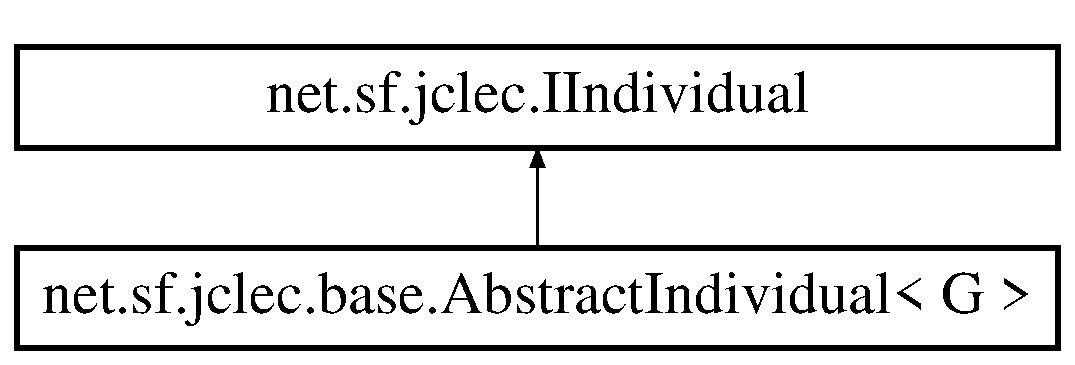
\includegraphics[height=2.000000cm]{classnet_1_1sf_1_1jclec_1_1base_1_1_abstract_individual_3_01_g_01_4}
\end{center}
\end{figure}
\subsection*{Public Member Functions}
\begin{DoxyCompactItemize}
\item 
final void \hyperlink{classnet_1_1sf_1_1jclec_1_1base_1_1_abstract_individual_3_01_g_01_4_a335c562b813e8b67ce18bd4d8da703ae}{set\-Genotype} (G \hyperlink{classnet_1_1sf_1_1jclec_1_1base_1_1_abstract_individual_3_01_g_01_4_a17532a6cefcacd7a913749d1f46d798c}{genotype})
\item 
final G \hyperlink{classnet_1_1sf_1_1jclec_1_1base_1_1_abstract_individual_3_01_g_01_4_aab0ec4944079f7b52dc834f8ed79024e}{get\-Genotype} ()
\item 
final \hyperlink{interfacenet_1_1sf_1_1jclec_1_1_i_fitness}{I\-Fitness} \hyperlink{classnet_1_1sf_1_1jclec_1_1base_1_1_abstract_individual_3_01_g_01_4_a0c7384db3b17214bff18ffcbbb21fda0}{get\-Fitness} ()
\item 
final void \hyperlink{classnet_1_1sf_1_1jclec_1_1base_1_1_abstract_individual_3_01_g_01_4_a99712eb48238ca6e13411cf2e68dc26b}{set\-Fitness} (\hyperlink{interfacenet_1_1sf_1_1jclec_1_1_i_fitness}{I\-Fitness} \hyperlink{classnet_1_1sf_1_1jclec_1_1base_1_1_abstract_individual_3_01_g_01_4_a333045009734aca2834c6a7fab508fa2}{fitness})
\item 
String \hyperlink{classnet_1_1sf_1_1jclec_1_1base_1_1_abstract_individual_3_01_g_01_4_a945e26198c23a9ffe41a46aa78a7d141}{to\-String} ()
\end{DoxyCompactItemize}
\subsection*{Protected Member Functions}
\begin{DoxyCompactItemize}
\item 
\hyperlink{classnet_1_1sf_1_1jclec_1_1base_1_1_abstract_individual_3_01_g_01_4_ae7aec40ca86c7c56c43ca5eeaccc4b5d}{Abstract\-Individual} ()
\item 
\hyperlink{classnet_1_1sf_1_1jclec_1_1base_1_1_abstract_individual_3_01_g_01_4_a908ad0362124170763a1a2863c92fd37}{Abstract\-Individual} (G \hyperlink{classnet_1_1sf_1_1jclec_1_1base_1_1_abstract_individual_3_01_g_01_4_a17532a6cefcacd7a913749d1f46d798c}{genotype})
\item 
\hyperlink{classnet_1_1sf_1_1jclec_1_1base_1_1_abstract_individual_3_01_g_01_4_aafb14fd653c117449a34de7a19c2758a}{Abstract\-Individual} (G \hyperlink{classnet_1_1sf_1_1jclec_1_1base_1_1_abstract_individual_3_01_g_01_4_a17532a6cefcacd7a913749d1f46d798c}{genotype}, \hyperlink{interfacenet_1_1sf_1_1jclec_1_1_i_fitness}{I\-Fitness} \hyperlink{classnet_1_1sf_1_1jclec_1_1base_1_1_abstract_individual_3_01_g_01_4_a333045009734aca2834c6a7fab508fa2}{fitness})
\end{DoxyCompactItemize}
\subsection*{Protected Attributes}
\begin{DoxyCompactItemize}
\item 
G \hyperlink{classnet_1_1sf_1_1jclec_1_1base_1_1_abstract_individual_3_01_g_01_4_a17532a6cefcacd7a913749d1f46d798c}{genotype}
\item 
\hyperlink{interfacenet_1_1sf_1_1jclec_1_1_i_fitness}{I\-Fitness} \hyperlink{classnet_1_1sf_1_1jclec_1_1base_1_1_abstract_individual_3_01_g_01_4_a333045009734aca2834c6a7fab508fa2}{fitness}
\end{DoxyCompactItemize}


\subsection{Detailed Description}
\hyperlink{interfacenet_1_1sf_1_1jclec_1_1_i_individual}{I\-Individual} abstract implementation.

\begin{DoxyAuthor}{Author}
Sebastian Ventura
\end{DoxyAuthor}

\begin{DoxyParams}{Parameters}
{\em $<$\-G$>$} & Object that plays the role of genotype \\
\hline
\end{DoxyParams}


\subsection{Constructor \& Destructor Documentation}
\hypertarget{classnet_1_1sf_1_1jclec_1_1base_1_1_abstract_individual_3_01_g_01_4_ae7aec40ca86c7c56c43ca5eeaccc4b5d}{\index{net\-::sf\-::jclec\-::base\-::\-Abstract\-Individual$<$ G $>$@{net\-::sf\-::jclec\-::base\-::\-Abstract\-Individual$<$ G $>$}!Abstract\-Individual@{Abstract\-Individual}}
\index{Abstract\-Individual@{Abstract\-Individual}!net::sf::jclec::base::AbstractIndividual< G >@{net\-::sf\-::jclec\-::base\-::\-Abstract\-Individual$<$ G $>$}}
\subsubsection[{Abstract\-Individual}]{\setlength{\rightskip}{0pt plus 5cm}net.\-sf.\-jclec.\-base.\-Abstract\-Individual$<$ G $>$.Abstract\-Individual (
\begin{DoxyParamCaption}
{}
\end{DoxyParamCaption}
)\hspace{0.3cm}{\ttfamily [protected]}}}\label{classnet_1_1sf_1_1jclec_1_1base_1_1_abstract_individual_3_01_g_01_4_ae7aec40ca86c7c56c43ca5eeaccc4b5d}
Empty constructor \hypertarget{classnet_1_1sf_1_1jclec_1_1base_1_1_abstract_individual_3_01_g_01_4_a908ad0362124170763a1a2863c92fd37}{\index{net\-::sf\-::jclec\-::base\-::\-Abstract\-Individual$<$ G $>$@{net\-::sf\-::jclec\-::base\-::\-Abstract\-Individual$<$ G $>$}!Abstract\-Individual@{Abstract\-Individual}}
\index{Abstract\-Individual@{Abstract\-Individual}!net::sf::jclec::base::AbstractIndividual< G >@{net\-::sf\-::jclec\-::base\-::\-Abstract\-Individual$<$ G $>$}}
\subsubsection[{Abstract\-Individual}]{\setlength{\rightskip}{0pt plus 5cm}net.\-sf.\-jclec.\-base.\-Abstract\-Individual$<$ G $>$.Abstract\-Individual (
\begin{DoxyParamCaption}
\item[{G}]{genotype}
\end{DoxyParamCaption}
)\hspace{0.3cm}{\ttfamily [protected]}}}\label{classnet_1_1sf_1_1jclec_1_1base_1_1_abstract_individual_3_01_g_01_4_a908ad0362124170763a1a2863c92fd37}
Constructor that sets individual genotype.


\begin{DoxyParams}{Parameters}
{\em genotype} & Individual genotype \\
\hline
\end{DoxyParams}
\hypertarget{classnet_1_1sf_1_1jclec_1_1base_1_1_abstract_individual_3_01_g_01_4_aafb14fd653c117449a34de7a19c2758a}{\index{net\-::sf\-::jclec\-::base\-::\-Abstract\-Individual$<$ G $>$@{net\-::sf\-::jclec\-::base\-::\-Abstract\-Individual$<$ G $>$}!Abstract\-Individual@{Abstract\-Individual}}
\index{Abstract\-Individual@{Abstract\-Individual}!net::sf::jclec::base::AbstractIndividual< G >@{net\-::sf\-::jclec\-::base\-::\-Abstract\-Individual$<$ G $>$}}
\subsubsection[{Abstract\-Individual}]{\setlength{\rightskip}{0pt plus 5cm}net.\-sf.\-jclec.\-base.\-Abstract\-Individual$<$ G $>$.Abstract\-Individual (
\begin{DoxyParamCaption}
\item[{G}]{genotype, }
\item[{{\bf I\-Fitness}}]{fitness}
\end{DoxyParamCaption}
)\hspace{0.3cm}{\ttfamily [protected]}}}\label{classnet_1_1sf_1_1jclec_1_1base_1_1_abstract_individual_3_01_g_01_4_aafb14fd653c117449a34de7a19c2758a}
Constructor that sets individual genotype and fitness.


\begin{DoxyParams}{Parameters}
{\em genotype} & Individual genotype \\
\hline
{\em fitness} & Individual fitness \\
\hline
\end{DoxyParams}


\subsection{Member Function Documentation}
\hypertarget{classnet_1_1sf_1_1jclec_1_1base_1_1_abstract_individual_3_01_g_01_4_a0c7384db3b17214bff18ffcbbb21fda0}{\index{net\-::sf\-::jclec\-::base\-::\-Abstract\-Individual$<$ G $>$@{net\-::sf\-::jclec\-::base\-::\-Abstract\-Individual$<$ G $>$}!get\-Fitness@{get\-Fitness}}
\index{get\-Fitness@{get\-Fitness}!net::sf::jclec::base::AbstractIndividual< G >@{net\-::sf\-::jclec\-::base\-::\-Abstract\-Individual$<$ G $>$}}
\subsubsection[{get\-Fitness}]{\setlength{\rightskip}{0pt plus 5cm}final {\bf I\-Fitness} net.\-sf.\-jclec.\-base.\-Abstract\-Individual$<$ G $>$.get\-Fitness (
\begin{DoxyParamCaption}
{}
\end{DoxyParamCaption}
)}}\label{classnet_1_1sf_1_1jclec_1_1base_1_1_abstract_individual_3_01_g_01_4_a0c7384db3b17214bff18ffcbbb21fda0}
Access to individual fitness.

\begin{DoxyReturn}{Returns}
Individual fitness
\end{DoxyReturn}
 

Implements \hyperlink{interfacenet_1_1sf_1_1jclec_1_1_i_individual_af2c6e6204a66c02848e2cfe3780a7948}{net.\-sf.\-jclec.\-I\-Individual}.

\hypertarget{classnet_1_1sf_1_1jclec_1_1base_1_1_abstract_individual_3_01_g_01_4_aab0ec4944079f7b52dc834f8ed79024e}{\index{net\-::sf\-::jclec\-::base\-::\-Abstract\-Individual$<$ G $>$@{net\-::sf\-::jclec\-::base\-::\-Abstract\-Individual$<$ G $>$}!get\-Genotype@{get\-Genotype}}
\index{get\-Genotype@{get\-Genotype}!net::sf::jclec::base::AbstractIndividual< G >@{net\-::sf\-::jclec\-::base\-::\-Abstract\-Individual$<$ G $>$}}
\subsubsection[{get\-Genotype}]{\setlength{\rightskip}{0pt plus 5cm}final G net.\-sf.\-jclec.\-base.\-Abstract\-Individual$<$ G $>$.get\-Genotype (
\begin{DoxyParamCaption}
{}
\end{DoxyParamCaption}
)}}\label{classnet_1_1sf_1_1jclec_1_1base_1_1_abstract_individual_3_01_g_01_4_aab0ec4944079f7b52dc834f8ed79024e}
Access to individual genotype

\begin{DoxyReturn}{Returns}
Individual genotype 
\end{DoxyReturn}
\hypertarget{classnet_1_1sf_1_1jclec_1_1base_1_1_abstract_individual_3_01_g_01_4_a99712eb48238ca6e13411cf2e68dc26b}{\index{net\-::sf\-::jclec\-::base\-::\-Abstract\-Individual$<$ G $>$@{net\-::sf\-::jclec\-::base\-::\-Abstract\-Individual$<$ G $>$}!set\-Fitness@{set\-Fitness}}
\index{set\-Fitness@{set\-Fitness}!net::sf::jclec::base::AbstractIndividual< G >@{net\-::sf\-::jclec\-::base\-::\-Abstract\-Individual$<$ G $>$}}
\subsubsection[{set\-Fitness}]{\setlength{\rightskip}{0pt plus 5cm}final void net.\-sf.\-jclec.\-base.\-Abstract\-Individual$<$ G $>$.set\-Fitness (
\begin{DoxyParamCaption}
\item[{{\bf I\-Fitness}}]{fitness}
\end{DoxyParamCaption}
)}}\label{classnet_1_1sf_1_1jclec_1_1base_1_1_abstract_individual_3_01_g_01_4_a99712eb48238ca6e13411cf2e68dc26b}
Sets the fitness of this individual.


\begin{DoxyParams}{Parameters}
{\em fitness} & New fitness value.\\
\hline
\end{DoxyParams}
 

Implements \hyperlink{interfacenet_1_1sf_1_1jclec_1_1_i_individual_ad3e70e2475909eff7fcc29659cb65c0b}{net.\-sf.\-jclec.\-I\-Individual}.

\hypertarget{classnet_1_1sf_1_1jclec_1_1base_1_1_abstract_individual_3_01_g_01_4_a335c562b813e8b67ce18bd4d8da703ae}{\index{net\-::sf\-::jclec\-::base\-::\-Abstract\-Individual$<$ G $>$@{net\-::sf\-::jclec\-::base\-::\-Abstract\-Individual$<$ G $>$}!set\-Genotype@{set\-Genotype}}
\index{set\-Genotype@{set\-Genotype}!net::sf::jclec::base::AbstractIndividual< G >@{net\-::sf\-::jclec\-::base\-::\-Abstract\-Individual$<$ G $>$}}
\subsubsection[{set\-Genotype}]{\setlength{\rightskip}{0pt plus 5cm}final void net.\-sf.\-jclec.\-base.\-Abstract\-Individual$<$ G $>$.set\-Genotype (
\begin{DoxyParamCaption}
\item[{G}]{genotype}
\end{DoxyParamCaption}
)}}\label{classnet_1_1sf_1_1jclec_1_1base_1_1_abstract_individual_3_01_g_01_4_a335c562b813e8b67ce18bd4d8da703ae}
Sets individual genotype


\begin{DoxyParams}{Parameters}
{\em genotype} & Individual genotype \\
\hline
\end{DoxyParams}
\hypertarget{classnet_1_1sf_1_1jclec_1_1base_1_1_abstract_individual_3_01_g_01_4_a945e26198c23a9ffe41a46aa78a7d141}{\index{net\-::sf\-::jclec\-::base\-::\-Abstract\-Individual$<$ G $>$@{net\-::sf\-::jclec\-::base\-::\-Abstract\-Individual$<$ G $>$}!to\-String@{to\-String}}
\index{to\-String@{to\-String}!net::sf::jclec::base::AbstractIndividual< G >@{net\-::sf\-::jclec\-::base\-::\-Abstract\-Individual$<$ G $>$}}
\subsubsection[{to\-String}]{\setlength{\rightskip}{0pt plus 5cm}String net.\-sf.\-jclec.\-base.\-Abstract\-Individual$<$ G $>$.to\-String (
\begin{DoxyParamCaption}
{}
\end{DoxyParamCaption}
)}}\label{classnet_1_1sf_1_1jclec_1_1base_1_1_abstract_individual_3_01_g_01_4_a945e26198c23a9ffe41a46aa78a7d141}
Return an string that represent this fitness object legibly.

\begin{DoxyReturn}{Returns}
String that represents this individual. 
\end{DoxyReturn}


\subsection{Member Data Documentation}
\hypertarget{classnet_1_1sf_1_1jclec_1_1base_1_1_abstract_individual_3_01_g_01_4_a333045009734aca2834c6a7fab508fa2}{\index{net\-::sf\-::jclec\-::base\-::\-Abstract\-Individual$<$ G $>$@{net\-::sf\-::jclec\-::base\-::\-Abstract\-Individual$<$ G $>$}!fitness@{fitness}}
\index{fitness@{fitness}!net::sf::jclec::base::AbstractIndividual< G >@{net\-::sf\-::jclec\-::base\-::\-Abstract\-Individual$<$ G $>$}}
\subsubsection[{fitness}]{\setlength{\rightskip}{0pt plus 5cm}{\bf I\-Fitness} net.\-sf.\-jclec.\-base.\-Abstract\-Individual$<$ G $>$.fitness\hspace{0.3cm}{\ttfamily [protected]}}}\label{classnet_1_1sf_1_1jclec_1_1base_1_1_abstract_individual_3_01_g_01_4_a333045009734aca2834c6a7fab508fa2}
Individual fitness \hypertarget{classnet_1_1sf_1_1jclec_1_1base_1_1_abstract_individual_3_01_g_01_4_a17532a6cefcacd7a913749d1f46d798c}{\index{net\-::sf\-::jclec\-::base\-::\-Abstract\-Individual$<$ G $>$@{net\-::sf\-::jclec\-::base\-::\-Abstract\-Individual$<$ G $>$}!genotype@{genotype}}
\index{genotype@{genotype}!net::sf::jclec::base::AbstractIndividual< G >@{net\-::sf\-::jclec\-::base\-::\-Abstract\-Individual$<$ G $>$}}
\subsubsection[{genotype}]{\setlength{\rightskip}{0pt plus 5cm}G net.\-sf.\-jclec.\-base.\-Abstract\-Individual$<$ G $>$.genotype\hspace{0.3cm}{\ttfamily [protected]}}}\label{classnet_1_1sf_1_1jclec_1_1base_1_1_abstract_individual_3_01_g_01_4_a17532a6cefcacd7a913749d1f46d798c}
Individual genotype 

The documentation for this class was generated from the following file\-:\begin{DoxyCompactItemize}
\item 
src/main/java/net/sf/jclec/base/Abstract\-Individual.\-java\end{DoxyCompactItemize}

\hypertarget{classnet_1_1sf_1_1jclec_1_1base_1_1_abstract_mutator}{\section{net.\-sf.\-jclec.\-base.\-Abstract\-Mutator Class Reference}
\label{classnet_1_1sf_1_1jclec_1_1base_1_1_abstract_mutator}\index{net.\-sf.\-jclec.\-base.\-Abstract\-Mutator@{net.\-sf.\-jclec.\-base.\-Abstract\-Mutator}}
}
Inheritance diagram for net.\-sf.\-jclec.\-base.\-Abstract\-Mutator\-:\begin{figure}[H]
\begin{center}
\leavevmode
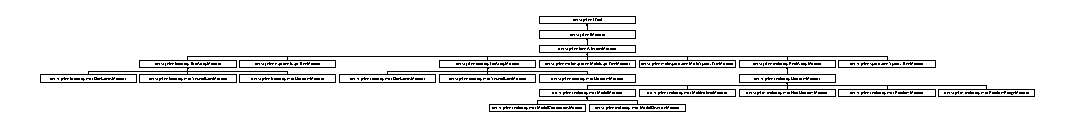
\includegraphics[height=1.276873cm]{classnet_1_1sf_1_1jclec_1_1base_1_1_abstract_mutator}
\end{center}
\end{figure}
\subsection*{Public Member Functions}
\begin{DoxyCompactItemize}
\item 
\hyperlink{classnet_1_1sf_1_1jclec_1_1base_1_1_abstract_mutator_a6ce8dd6a6cdcc19c003e7f40f0af9e54}{Abstract\-Mutator} ()
\item 
final void \hyperlink{classnet_1_1sf_1_1jclec_1_1base_1_1_abstract_mutator_a09e2996e9f6715d658b07d41971801c8}{contextualize} (\hyperlink{interfacenet_1_1sf_1_1jclec_1_1_i_system}{I\-System} \hyperlink{classnet_1_1sf_1_1jclec_1_1base_1_1_abstract_mutator_af0995dc3ca644cea60e43aa65085f097}{context})
\item 
List$<$ \hyperlink{interfacenet_1_1sf_1_1jclec_1_1_i_individual}{I\-Individual} $>$ \hyperlink{classnet_1_1sf_1_1jclec_1_1base_1_1_abstract_mutator_a6dc5e2ae8e27cdda9639cad2cadd6fba}{mutate} (List$<$ \hyperlink{interfacenet_1_1sf_1_1jclec_1_1_i_individual}{I\-Individual} $>$ parents)
\end{DoxyCompactItemize}
\subsection*{Protected Member Functions}
\begin{DoxyCompactItemize}
\item 
abstract void \hyperlink{classnet_1_1sf_1_1jclec_1_1base_1_1_abstract_mutator_ad12e6a2be8fb6082255ce8f399c9b166}{prepare\-Mutation} ()
\item 
abstract void \hyperlink{classnet_1_1sf_1_1jclec_1_1base_1_1_abstract_mutator_acad18bae2458fe06812b321d43f3499e}{mutate\-Next} ()
\end{DoxyCompactItemize}
\subsection*{Protected Attributes}
\begin{DoxyCompactItemize}
\item 
\hyperlink{interfacenet_1_1sf_1_1jclec_1_1_i_population}{I\-Population} \hyperlink{classnet_1_1sf_1_1jclec_1_1base_1_1_abstract_mutator_af0995dc3ca644cea60e43aa65085f097}{context}
\item 
\hyperlink{interfacenet_1_1sf_1_1jclec_1_1util_1_1random_1_1_i_rand_gen}{I\-Rand\-Gen} \hyperlink{classnet_1_1sf_1_1jclec_1_1base_1_1_abstract_mutator_a21907b5345c3af80722235d42aec079a}{randgen}
\item 
transient List$<$ \hyperlink{interfacenet_1_1sf_1_1jclec_1_1_i_individual}{I\-Individual} $>$ \hyperlink{classnet_1_1sf_1_1jclec_1_1base_1_1_abstract_mutator_a246b0bbd581762861efb3e2da0e68d3f}{parents\-Buffer}
\item 
transient List$<$ \hyperlink{interfacenet_1_1sf_1_1jclec_1_1_i_individual}{I\-Individual} $>$ \hyperlink{classnet_1_1sf_1_1jclec_1_1base_1_1_abstract_mutator_ab44190f45865606f8d385b50a7863c35}{sons\-Buffer}
\item 
transient int \hyperlink{classnet_1_1sf_1_1jclec_1_1base_1_1_abstract_mutator_ad1bc7a6bb4e3be8e6aae039c7bb5d8d8}{parents\-Counter}
\end{DoxyCompactItemize}


\subsection{Detailed Description}
\hyperlink{interfacenet_1_1sf_1_1jclec_1_1_i_mutator}{I\-Mutator} abstract implementation.

\begin{DoxyAuthor}{Author}
Sebastian Ventura 
\end{DoxyAuthor}


\subsection{Constructor \& Destructor Documentation}
\hypertarget{classnet_1_1sf_1_1jclec_1_1base_1_1_abstract_mutator_a6ce8dd6a6cdcc19c003e7f40f0af9e54}{\index{net\-::sf\-::jclec\-::base\-::\-Abstract\-Mutator@{net\-::sf\-::jclec\-::base\-::\-Abstract\-Mutator}!Abstract\-Mutator@{Abstract\-Mutator}}
\index{Abstract\-Mutator@{Abstract\-Mutator}!net::sf::jclec::base::AbstractMutator@{net\-::sf\-::jclec\-::base\-::\-Abstract\-Mutator}}
\subsubsection[{Abstract\-Mutator}]{\setlength{\rightskip}{0pt plus 5cm}net.\-sf.\-jclec.\-base.\-Abstract\-Mutator.\-Abstract\-Mutator (
\begin{DoxyParamCaption}
{}
\end{DoxyParamCaption}
)}}\label{classnet_1_1sf_1_1jclec_1_1base_1_1_abstract_mutator_a6ce8dd6a6cdcc19c003e7f40f0af9e54}
Empty constructor. 

\subsection{Member Function Documentation}
\hypertarget{classnet_1_1sf_1_1jclec_1_1base_1_1_abstract_mutator_a09e2996e9f6715d658b07d41971801c8}{\index{net\-::sf\-::jclec\-::base\-::\-Abstract\-Mutator@{net\-::sf\-::jclec\-::base\-::\-Abstract\-Mutator}!contextualize@{contextualize}}
\index{contextualize@{contextualize}!net::sf::jclec::base::AbstractMutator@{net\-::sf\-::jclec\-::base\-::\-Abstract\-Mutator}}
\subsubsection[{contextualize}]{\setlength{\rightskip}{0pt plus 5cm}final void net.\-sf.\-jclec.\-base.\-Abstract\-Mutator.\-contextualize (
\begin{DoxyParamCaption}
\item[{{\bf I\-System}}]{context}
\end{DoxyParamCaption}
)}}\label{classnet_1_1sf_1_1jclec_1_1base_1_1_abstract_mutator_a09e2996e9f6715d658b07d41971801c8}
Set the system where ...


\begin{DoxyParams}{Parameters}
{\em context} & Execution context\\
\hline
\end{DoxyParams}
 

Implements \hyperlink{interfacenet_1_1sf_1_1jclec_1_1_i_tool_aa11b3e046b7f38e40eb4f8c72a9a2102}{net.\-sf.\-jclec.\-I\-Tool}.

\hypertarget{classnet_1_1sf_1_1jclec_1_1base_1_1_abstract_mutator_a6dc5e2ae8e27cdda9639cad2cadd6fba}{\index{net\-::sf\-::jclec\-::base\-::\-Abstract\-Mutator@{net\-::sf\-::jclec\-::base\-::\-Abstract\-Mutator}!mutate@{mutate}}
\index{mutate@{mutate}!net::sf::jclec::base::AbstractMutator@{net\-::sf\-::jclec\-::base\-::\-Abstract\-Mutator}}
\subsubsection[{mutate}]{\setlength{\rightskip}{0pt plus 5cm}List$<${\bf I\-Individual}$>$ net.\-sf.\-jclec.\-base.\-Abstract\-Mutator.\-mutate (
\begin{DoxyParamCaption}
\item[{List$<$ {\bf I\-Individual} $>$}]{parents}
\end{DoxyParamCaption}
)}}\label{classnet_1_1sf_1_1jclec_1_1base_1_1_abstract_mutator_a6dc5e2ae8e27cdda9639cad2cadd6fba}
Mutation method.


\begin{DoxyParams}{Parameters}
{\em parents} & Individuals to mutate\\
\hline
\end{DoxyParams}
\begin{DoxyReturn}{Returns}
Mutation result
\end{DoxyReturn}
 

Implements \hyperlink{interfacenet_1_1sf_1_1jclec_1_1_i_mutator_a5300cd0df63950ea9f660b24425211fb}{net.\-sf.\-jclec.\-I\-Mutator}.

\hypertarget{classnet_1_1sf_1_1jclec_1_1base_1_1_abstract_mutator_acad18bae2458fe06812b321d43f3499e}{\index{net\-::sf\-::jclec\-::base\-::\-Abstract\-Mutator@{net\-::sf\-::jclec\-::base\-::\-Abstract\-Mutator}!mutate\-Next@{mutate\-Next}}
\index{mutate\-Next@{mutate\-Next}!net::sf::jclec::base::AbstractMutator@{net\-::sf\-::jclec\-::base\-::\-Abstract\-Mutator}}
\subsubsection[{mutate\-Next}]{\setlength{\rightskip}{0pt plus 5cm}abstract void net.\-sf.\-jclec.\-base.\-Abstract\-Mutator.\-mutate\-Next (
\begin{DoxyParamCaption}
{}
\end{DoxyParamCaption}
)\hspace{0.3cm}{\ttfamily [protected]}, {\ttfamily [pure virtual]}}}\label{classnet_1_1sf_1_1jclec_1_1base_1_1_abstract_mutator_acad18bae2458fe06812b321d43f3499e}
Atomic mutation method. This method... 

Implemented in \hyperlink{classnet_1_1sf_1_1jclec_1_1intarray_1_1mut_1_1_several_loci_mutator_a8e834b186164c7ad895464699a10941e}{net.\-sf.\-jclec.\-intarray.\-mut.\-Several\-Loci\-Mutator}, \hyperlink{classnet_1_1sf_1_1jclec_1_1binarray_1_1mut_1_1_several_loci_mutator_a9d195623cf89f738b53940a082059a24}{net.\-sf.\-jclec.\-binarray.\-mut.\-Several\-Loci\-Mutator}, \hyperlink{classnet_1_1sf_1_1jclec_1_1multisyntaxtree_1_1_multi_syntax_tree_mutator_a639c8a190fed6f77db9844dfce7a4f6c}{net.\-sf.\-jclec.\-multisyntaxtree.\-Multi\-Syntax\-Tree\-Mutator}, \hyperlink{classnet_1_1sf_1_1jclec_1_1multiexprtree_1_1_multi_expr_tree_mutator_a4a3637da6427be21eb5804a45f0a2ce7}{net.\-sf.\-jclec.\-multiexprtree.\-Multi\-Expr\-Tree\-Mutator}, \hyperlink{classnet_1_1sf_1_1jclec_1_1intarray_1_1mut_1_1_uniform_mutator_ac35f3eec57a49484815855ed1db9a2da}{net.\-sf.\-jclec.\-intarray.\-mut.\-Uniform\-Mutator}, \hyperlink{classnet_1_1sf_1_1jclec_1_1syntaxtree_1_1_syntax_tree_mutator_a74e5f24fa1234791cb3e242c5426f9e8}{net.\-sf.\-jclec.\-syntaxtree.\-Syntax\-Tree\-Mutator}, \hyperlink{classnet_1_1sf_1_1jclec_1_1binarray_1_1mut_1_1_uniform_mutator_ad631a7f477c8af9a61b8fdb64d61e9bd}{net.\-sf.\-jclec.\-binarray.\-mut.\-Uniform\-Mutator}, \hyperlink{classnet_1_1sf_1_1jclec_1_1exprtree_1_1_expr_tree_mutator_a51f55d91527bfbd7656f6cd11c4ebb3d}{net.\-sf.\-jclec.\-exprtree.\-Expr\-Tree\-Mutator}, \hyperlink{classnet_1_1sf_1_1jclec_1_1realarray_1_1_uniform_mutator_a7c90fd0f74afd20e102f9cbf87014e9b}{net.\-sf.\-jclec.\-realarray.\-Uniform\-Mutator}, \hyperlink{classnet_1_1sf_1_1jclec_1_1binarray_1_1mut_1_1_one_locus_mutator_afcbf5c30ec1b952e34b188659d7bd470}{net.\-sf.\-jclec.\-binarray.\-mut.\-One\-Locus\-Mutator}, and \hyperlink{classnet_1_1sf_1_1jclec_1_1intarray_1_1mut_1_1_one_locus_mutator_ad4a1be2de8902dc1153d7f0ed57132f7}{net.\-sf.\-jclec.\-intarray.\-mut.\-One\-Locus\-Mutator}.

\hypertarget{classnet_1_1sf_1_1jclec_1_1base_1_1_abstract_mutator_ad12e6a2be8fb6082255ce8f399c9b166}{\index{net\-::sf\-::jclec\-::base\-::\-Abstract\-Mutator@{net\-::sf\-::jclec\-::base\-::\-Abstract\-Mutator}!prepare\-Mutation@{prepare\-Mutation}}
\index{prepare\-Mutation@{prepare\-Mutation}!net::sf::jclec::base::AbstractMutator@{net\-::sf\-::jclec\-::base\-::\-Abstract\-Mutator}}
\subsubsection[{prepare\-Mutation}]{\setlength{\rightskip}{0pt plus 5cm}abstract void net.\-sf.\-jclec.\-base.\-Abstract\-Mutator.\-prepare\-Mutation (
\begin{DoxyParamCaption}
{}
\end{DoxyParamCaption}
)\hspace{0.3cm}{\ttfamily [protected]}, {\ttfamily [pure virtual]}}}\label{classnet_1_1sf_1_1jclec_1_1base_1_1_abstract_mutator_ad12e6a2be8fb6082255ce8f399c9b166}
Prepare mutation process. 

Implemented in \hyperlink{classnet_1_1sf_1_1jclec_1_1realarray_1_1mut_1_1_non_uniform_mutator_af0c404dbbc03b506c7517729bd479181}{net.\-sf.\-jclec.\-realarray.\-mut.\-Non\-Uniform\-Mutator}, \hyperlink{classnet_1_1sf_1_1jclec_1_1multisyntaxtree_1_1_multi_syntax_tree_mutator_abc579c6ab91161c80f75e2f643b864ac}{net.\-sf.\-jclec.\-multisyntaxtree.\-Multi\-Syntax\-Tree\-Mutator}, \hyperlink{classnet_1_1sf_1_1jclec_1_1multiexprtree_1_1_multi_expr_tree_mutator_a0793d815841d004beaaa9acb66659e87}{net.\-sf.\-jclec.\-multiexprtree.\-Multi\-Expr\-Tree\-Mutator}, \hyperlink{classnet_1_1sf_1_1jclec_1_1syntaxtree_1_1_syntax_tree_mutator_a89e6a223695258e4f7e42edb54a4e077}{net.\-sf.\-jclec.\-syntaxtree.\-Syntax\-Tree\-Mutator}, \hyperlink{classnet_1_1sf_1_1jclec_1_1exprtree_1_1_expr_tree_mutator_a2bafce5d54003041106517857e0ce65b}{net.\-sf.\-jclec.\-exprtree.\-Expr\-Tree\-Mutator}, \hyperlink{classnet_1_1sf_1_1jclec_1_1realarray_1_1mut_1_1_modal_continuous_mutator_a7e418455e1ce51a13043d748d032a17d}{net.\-sf.\-jclec.\-realarray.\-mut.\-Modal\-Continuous\-Mutator}, \hyperlink{classnet_1_1sf_1_1jclec_1_1realarray_1_1_real_array_mutator_a6fbfa9c56e7c6e3af8532636dd0ceb60}{net.\-sf.\-jclec.\-realarray.\-Real\-Array\-Mutator}, \hyperlink{classnet_1_1sf_1_1jclec_1_1intarray_1_1_int_array_mutator_a088c3c1163c64a669a623c949843cd15}{net.\-sf.\-jclec.\-intarray.\-Int\-Array\-Mutator}, and \hyperlink{classnet_1_1sf_1_1jclec_1_1binarray_1_1_bin_array_mutator_a104587c4458bc8c299cdf902e0ee0cc9}{net.\-sf.\-jclec.\-binarray.\-Bin\-Array\-Mutator}.



\subsection{Member Data Documentation}
\hypertarget{classnet_1_1sf_1_1jclec_1_1base_1_1_abstract_mutator_af0995dc3ca644cea60e43aa65085f097}{\index{net\-::sf\-::jclec\-::base\-::\-Abstract\-Mutator@{net\-::sf\-::jclec\-::base\-::\-Abstract\-Mutator}!context@{context}}
\index{context@{context}!net::sf::jclec::base::AbstractMutator@{net\-::sf\-::jclec\-::base\-::\-Abstract\-Mutator}}
\subsubsection[{context}]{\setlength{\rightskip}{0pt plus 5cm}{\bf I\-Population} net.\-sf.\-jclec.\-base.\-Abstract\-Mutator.\-context\hspace{0.3cm}{\ttfamily [protected]}}}\label{classnet_1_1sf_1_1jclec_1_1base_1_1_abstract_mutator_af0995dc3ca644cea60e43aa65085f097}
Execution context \hypertarget{classnet_1_1sf_1_1jclec_1_1base_1_1_abstract_mutator_a246b0bbd581762861efb3e2da0e68d3f}{\index{net\-::sf\-::jclec\-::base\-::\-Abstract\-Mutator@{net\-::sf\-::jclec\-::base\-::\-Abstract\-Mutator}!parents\-Buffer@{parents\-Buffer}}
\index{parents\-Buffer@{parents\-Buffer}!net::sf::jclec::base::AbstractMutator@{net\-::sf\-::jclec\-::base\-::\-Abstract\-Mutator}}
\subsubsection[{parents\-Buffer}]{\setlength{\rightskip}{0pt plus 5cm}transient List$<${\bf I\-Individual}$>$ net.\-sf.\-jclec.\-base.\-Abstract\-Mutator.\-parents\-Buffer\hspace{0.3cm}{\ttfamily [protected]}}}\label{classnet_1_1sf_1_1jclec_1_1base_1_1_abstract_mutator_a246b0bbd581762861efb3e2da0e68d3f}
Parents buffer. Used by the atomic mutation method \hypertarget{classnet_1_1sf_1_1jclec_1_1base_1_1_abstract_mutator_ad1bc7a6bb4e3be8e6aae039c7bb5d8d8}{\index{net\-::sf\-::jclec\-::base\-::\-Abstract\-Mutator@{net\-::sf\-::jclec\-::base\-::\-Abstract\-Mutator}!parents\-Counter@{parents\-Counter}}
\index{parents\-Counter@{parents\-Counter}!net::sf::jclec::base::AbstractMutator@{net\-::sf\-::jclec\-::base\-::\-Abstract\-Mutator}}
\subsubsection[{parents\-Counter}]{\setlength{\rightskip}{0pt plus 5cm}transient int net.\-sf.\-jclec.\-base.\-Abstract\-Mutator.\-parents\-Counter\hspace{0.3cm}{\ttfamily [protected]}}}\label{classnet_1_1sf_1_1jclec_1_1base_1_1_abstract_mutator_ad1bc7a6bb4e3be8e6aae039c7bb5d8d8}
Parent counter \hypertarget{classnet_1_1sf_1_1jclec_1_1base_1_1_abstract_mutator_a21907b5345c3af80722235d42aec079a}{\index{net\-::sf\-::jclec\-::base\-::\-Abstract\-Mutator@{net\-::sf\-::jclec\-::base\-::\-Abstract\-Mutator}!randgen@{randgen}}
\index{randgen@{randgen}!net::sf::jclec::base::AbstractMutator@{net\-::sf\-::jclec\-::base\-::\-Abstract\-Mutator}}
\subsubsection[{randgen}]{\setlength{\rightskip}{0pt plus 5cm}{\bf I\-Rand\-Gen} net.\-sf.\-jclec.\-base.\-Abstract\-Mutator.\-randgen\hspace{0.3cm}{\ttfamily [protected]}}}\label{classnet_1_1sf_1_1jclec_1_1base_1_1_abstract_mutator_a21907b5345c3af80722235d42aec079a}
Random generator used in mutation \hypertarget{classnet_1_1sf_1_1jclec_1_1base_1_1_abstract_mutator_ab44190f45865606f8d385b50a7863c35}{\index{net\-::sf\-::jclec\-::base\-::\-Abstract\-Mutator@{net\-::sf\-::jclec\-::base\-::\-Abstract\-Mutator}!sons\-Buffer@{sons\-Buffer}}
\index{sons\-Buffer@{sons\-Buffer}!net::sf::jclec::base::AbstractMutator@{net\-::sf\-::jclec\-::base\-::\-Abstract\-Mutator}}
\subsubsection[{sons\-Buffer}]{\setlength{\rightskip}{0pt plus 5cm}transient List$<${\bf I\-Individual}$>$ net.\-sf.\-jclec.\-base.\-Abstract\-Mutator.\-sons\-Buffer\hspace{0.3cm}{\ttfamily [protected]}}}\label{classnet_1_1sf_1_1jclec_1_1base_1_1_abstract_mutator_ab44190f45865606f8d385b50a7863c35}
Sons buffer. Used by the atomic mutation method 

The documentation for this class was generated from the following file\-:\begin{DoxyCompactItemize}
\item 
src/main/java/net/sf/jclec/base/Abstract\-Mutator.\-java\end{DoxyCompactItemize}

\hypertarget{classnet_1_1sf_1_1jclec_1_1base_1_1_abstract_parallel_evaluator}{\section{net.\-sf.\-jclec.\-base.\-Abstract\-Parallel\-Evaluator Class Reference}
\label{classnet_1_1sf_1_1jclec_1_1base_1_1_abstract_parallel_evaluator}\index{net.\-sf.\-jclec.\-base.\-Abstract\-Parallel\-Evaluator@{net.\-sf.\-jclec.\-base.\-Abstract\-Parallel\-Evaluator}}
}
Inheritance diagram for net.\-sf.\-jclec.\-base.\-Abstract\-Parallel\-Evaluator\-:\begin{figure}[H]
\begin{center}
\leavevmode
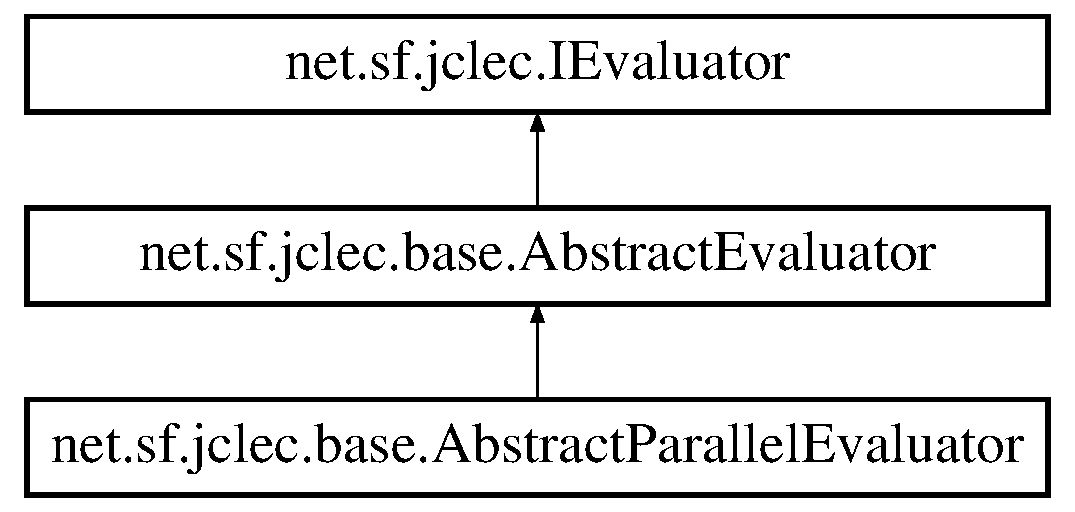
\includegraphics[height=4.000000cm]{classnet_1_1sf_1_1jclec_1_1base_1_1_abstract_parallel_evaluator}
\end{center}
\end{figure}
\subsection*{Public Member Functions}
\begin{DoxyCompactItemize}
\item 
\hyperlink{classnet_1_1sf_1_1jclec_1_1base_1_1_abstract_parallel_evaluator_aff72218d817d0e002950fc43b7d223fe}{Abstract\-Parallel\-Evaluator} ()
\item 
void \hyperlink{classnet_1_1sf_1_1jclec_1_1base_1_1_abstract_parallel_evaluator_a56032c17683595e1667391594a31103d}{evaluate} (List$<$ \hyperlink{interfacenet_1_1sf_1_1jclec_1_1_i_individual}{I\-Individual} $>$ inds)
\end{DoxyCompactItemize}
\subsection*{Additional Inherited Members}


\subsection{Detailed Description}
\hyperlink{interfacenet_1_1sf_1_1jclec_1_1_i_evaluator}{I\-Evaluator} parallel abstract implementation.

\begin{DoxyAuthor}{Author}
Alberto Cano 

Sebastian Ventura 
\end{DoxyAuthor}


\subsection{Constructor \& Destructor Documentation}
\hypertarget{classnet_1_1sf_1_1jclec_1_1base_1_1_abstract_parallel_evaluator_aff72218d817d0e002950fc43b7d223fe}{\index{net\-::sf\-::jclec\-::base\-::\-Abstract\-Parallel\-Evaluator@{net\-::sf\-::jclec\-::base\-::\-Abstract\-Parallel\-Evaluator}!Abstract\-Parallel\-Evaluator@{Abstract\-Parallel\-Evaluator}}
\index{Abstract\-Parallel\-Evaluator@{Abstract\-Parallel\-Evaluator}!net::sf::jclec::base::AbstractParallelEvaluator@{net\-::sf\-::jclec\-::base\-::\-Abstract\-Parallel\-Evaluator}}
\subsubsection[{Abstract\-Parallel\-Evaluator}]{\setlength{\rightskip}{0pt plus 5cm}net.\-sf.\-jclec.\-base.\-Abstract\-Parallel\-Evaluator.\-Abstract\-Parallel\-Evaluator (
\begin{DoxyParamCaption}
{}
\end{DoxyParamCaption}
)}}\label{classnet_1_1sf_1_1jclec_1_1base_1_1_abstract_parallel_evaluator_aff72218d817d0e002950fc43b7d223fe}
Empty constructor. 

\subsection{Member Function Documentation}
\hypertarget{classnet_1_1sf_1_1jclec_1_1base_1_1_abstract_parallel_evaluator_a56032c17683595e1667391594a31103d}{\index{net\-::sf\-::jclec\-::base\-::\-Abstract\-Parallel\-Evaluator@{net\-::sf\-::jclec\-::base\-::\-Abstract\-Parallel\-Evaluator}!evaluate@{evaluate}}
\index{evaluate@{evaluate}!net::sf::jclec::base::AbstractParallelEvaluator@{net\-::sf\-::jclec\-::base\-::\-Abstract\-Parallel\-Evaluator}}
\subsubsection[{evaluate}]{\setlength{\rightskip}{0pt plus 5cm}void net.\-sf.\-jclec.\-base.\-Abstract\-Parallel\-Evaluator.\-evaluate (
\begin{DoxyParamCaption}
\item[{List$<$ {\bf I\-Individual} $>$}]{inds}
\end{DoxyParamCaption}
)}}\label{classnet_1_1sf_1_1jclec_1_1base_1_1_abstract_parallel_evaluator_a56032c17683595e1667391594a31103d}
For all individuals in \char`\"{}inds\char`\"{} array\-: if individual fitness is null, then evaluate this individual.

This method is final. Is anyone wants implement this method in another way should create a new \hyperlink{interfacenet_1_1sf_1_1jclec_1_1_i_evaluator}{I\-Evaluator} class.

Evaluation method.


\begin{DoxyParams}{Parameters}
{\em inds} & Individuals to evaluate\\
\hline
\end{DoxyParams}
 

Implements \hyperlink{interfacenet_1_1sf_1_1jclec_1_1_i_evaluator_a6a64b0d69f99da5be8a6c5b01c7752c2}{net.\-sf.\-jclec.\-I\-Evaluator}.



The documentation for this class was generated from the following file\-:\begin{DoxyCompactItemize}
\item 
src/main/java/net/sf/jclec/base/Abstract\-Parallel\-Evaluator.\-java\end{DoxyCompactItemize}

\hypertarget{classnet_1_1sf_1_1jclec_1_1exprtree_1_1fun_1_1_abstract_primitive}{\section{net.\-sf.\-jclec.\-exprtree.\-fun.\-Abstract\-Primitive Class Reference}
\label{classnet_1_1sf_1_1jclec_1_1exprtree_1_1fun_1_1_abstract_primitive}\index{net.\-sf.\-jclec.\-exprtree.\-fun.\-Abstract\-Primitive@{net.\-sf.\-jclec.\-exprtree.\-fun.\-Abstract\-Primitive}}
}
Inheritance diagram for net.\-sf.\-jclec.\-exprtree.\-fun.\-Abstract\-Primitive\-:\begin{figure}[H]
\begin{center}
\leavevmode
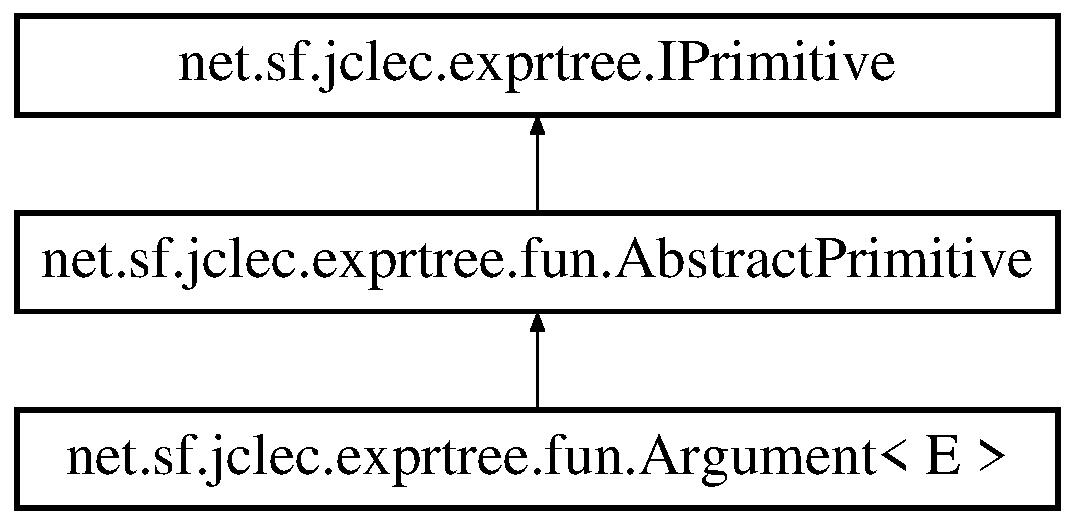
\includegraphics[height=3.000000cm]{classnet_1_1sf_1_1jclec_1_1exprtree_1_1fun_1_1_abstract_primitive}
\end{center}
\end{figure}
\subsection*{Public Member Functions}
\begin{DoxyCompactItemize}
\item 
final Class$<$?$>$\mbox{[}$\,$\mbox{]} \hyperlink{classnet_1_1sf_1_1jclec_1_1exprtree_1_1fun_1_1_abstract_primitive_a2f87e83f4dded5ff4a2278bbda54259c}{argument\-Types} ()
\item 
final Class$<$?$>$ \hyperlink{classnet_1_1sf_1_1jclec_1_1exprtree_1_1fun_1_1_abstract_primitive_ac3a0a1d9c1dd4935186976e6682c6acc}{return\-Type} ()
\item 
\hyperlink{interfacenet_1_1sf_1_1jclec_1_1exprtree_1_1_i_primitive}{I\-Primitive} \hyperlink{classnet_1_1sf_1_1jclec_1_1exprtree_1_1fun_1_1_abstract_primitive_ae38668f23b7b6d0833297ec42d9c48ee}{copy} ()
\item 
\hyperlink{interfacenet_1_1sf_1_1jclec_1_1exprtree_1_1_i_primitive}{I\-Primitive} \hyperlink{classnet_1_1sf_1_1jclec_1_1exprtree_1_1fun_1_1_abstract_primitive_acf7385b0b8a3f1405fe81bddddef8d1f}{instance} ()
\item 
final void \hyperlink{classnet_1_1sf_1_1jclec_1_1exprtree_1_1fun_1_1_abstract_primitive_a384b3d3dfc3841ea12ccfe06dd328c85}{evaluate} (\hyperlink{interfacenet_1_1sf_1_1jclec_1_1exprtree_1_1_i_context}{I\-Context} context)
\end{DoxyCompactItemize}
\subsection*{Protected Member Functions}
\begin{DoxyCompactItemize}
\item 
\hyperlink{classnet_1_1sf_1_1jclec_1_1exprtree_1_1fun_1_1_abstract_primitive_a9524b86b2835da7bdf83ff4fe51cae8f}{Abstract\-Primitive} (Class$<$?$>$\mbox{[}$\,$\mbox{]} atypes, Class$<$?$>$ rtype)
\item 
abstract void \hyperlink{classnet_1_1sf_1_1jclec_1_1exprtree_1_1fun_1_1_abstract_primitive_aab695f920997a9f1d873ab9b6f3ca246}{evaluate} (\hyperlink{classnet_1_1sf_1_1jclec_1_1exprtree_1_1fun_1_1_expr_tree_function}{Expr\-Tree\-Function} context)
\item 
void \hyperlink{classnet_1_1sf_1_1jclec_1_1exprtree_1_1fun_1_1_abstract_primitive_acf8deec8d668bba6dffe1562c7323580}{clear} (\hyperlink{classnet_1_1sf_1_1jclec_1_1exprtree_1_1fun_1_1_expr_tree_function}{Expr\-Tree\-Function} context)
\item 
void \hyperlink{classnet_1_1sf_1_1jclec_1_1exprtree_1_1fun_1_1_abstract_primitive_ab949217ef353c47de03730e0e63890ef}{push} (\hyperlink{classnet_1_1sf_1_1jclec_1_1exprtree_1_1fun_1_1_expr_tree_function}{Expr\-Tree\-Function} context, Object object)
\item 
Object\mbox{[}$\,$\mbox{]} \hyperlink{classnet_1_1sf_1_1jclec_1_1exprtree_1_1fun_1_1_abstract_primitive_a538b47566b8f08650cf367adad093432}{get\-Args} (\hyperlink{classnet_1_1sf_1_1jclec_1_1exprtree_1_1fun_1_1_expr_tree_function}{Expr\-Tree\-Function} context)
\item 
void \hyperlink{classnet_1_1sf_1_1jclec_1_1exprtree_1_1fun_1_1_abstract_primitive_ae925715073c8db3caa48f1470ee377e1}{push\-Arg} (\hyperlink{classnet_1_1sf_1_1jclec_1_1exprtree_1_1fun_1_1_expr_tree_function}{Expr\-Tree\-Function} context, int argindex)
\end{DoxyCompactItemize}
\subsection*{Protected Attributes}
\begin{DoxyCompactItemize}
\item 
final Class$<$?$>$\mbox{[}$\,$\mbox{]} \hyperlink{classnet_1_1sf_1_1jclec_1_1exprtree_1_1fun_1_1_abstract_primitive_a5c366872f0b89c0ae45f08207c57f2de}{arg\-Types}
\item 
final Class$<$?$>$ \hyperlink{classnet_1_1sf_1_1jclec_1_1exprtree_1_1fun_1_1_abstract_primitive_adc55259ee3939d073f17e70ddb428491}{return\-Type}
\end{DoxyCompactItemize}


\subsection{Detailed Description}
\hyperlink{interfacenet_1_1sf_1_1jclec_1_1exprtree_1_1_i_primitive}{I\-Primitive} abstract implementation

\begin{DoxyAuthor}{Author}
Sebastian Ventura 
\end{DoxyAuthor}


\subsection{Constructor \& Destructor Documentation}
\hypertarget{classnet_1_1sf_1_1jclec_1_1exprtree_1_1fun_1_1_abstract_primitive_a9524b86b2835da7bdf83ff4fe51cae8f}{\index{net\-::sf\-::jclec\-::exprtree\-::fun\-::\-Abstract\-Primitive@{net\-::sf\-::jclec\-::exprtree\-::fun\-::\-Abstract\-Primitive}!Abstract\-Primitive@{Abstract\-Primitive}}
\index{Abstract\-Primitive@{Abstract\-Primitive}!net::sf::jclec::exprtree::fun::AbstractPrimitive@{net\-::sf\-::jclec\-::exprtree\-::fun\-::\-Abstract\-Primitive}}
\subsubsection[{Abstract\-Primitive}]{\setlength{\rightskip}{0pt plus 5cm}net.\-sf.\-jclec.\-exprtree.\-fun.\-Abstract\-Primitive.\-Abstract\-Primitive (
\begin{DoxyParamCaption}
\item[{Class$<$?$>$\mbox{[}$\,$\mbox{]}}]{atypes, }
\item[{Class$<$?$>$}]{rtype}
\end{DoxyParamCaption}
)\hspace{0.3cm}{\ttfamily [protected]}}}\label{classnet_1_1sf_1_1jclec_1_1exprtree_1_1fun_1_1_abstract_primitive_a9524b86b2835da7bdf83ff4fe51cae8f}
Default constructor.

Subclasses of \hyperlink{classnet_1_1sf_1_1jclec_1_1exprtree_1_1fun_1_1_abstract_primitive}{Abstract\-Primitive} set argument and return types 

\subsection{Member Function Documentation}
\hypertarget{classnet_1_1sf_1_1jclec_1_1exprtree_1_1fun_1_1_abstract_primitive_a2f87e83f4dded5ff4a2278bbda54259c}{\index{net\-::sf\-::jclec\-::exprtree\-::fun\-::\-Abstract\-Primitive@{net\-::sf\-::jclec\-::exprtree\-::fun\-::\-Abstract\-Primitive}!argument\-Types@{argument\-Types}}
\index{argument\-Types@{argument\-Types}!net::sf::jclec::exprtree::fun::AbstractPrimitive@{net\-::sf\-::jclec\-::exprtree\-::fun\-::\-Abstract\-Primitive}}
\subsubsection[{argument\-Types}]{\setlength{\rightskip}{0pt plus 5cm}final Class$<$?$>$ \mbox{[}$\,$\mbox{]} net.\-sf.\-jclec.\-exprtree.\-fun.\-Abstract\-Primitive.\-argument\-Types (
\begin{DoxyParamCaption}
{}
\end{DoxyParamCaption}
)}}\label{classnet_1_1sf_1_1jclec_1_1exprtree_1_1fun_1_1_abstract_primitive_a2f87e83f4dded5ff4a2278bbda54259c}
Argument types for this primitive. If this is a terminal, this method returns an empty Class$<$?$>$ array.

\begin{DoxyReturn}{Returns}
Argument types for this primitive. 
\end{DoxyReturn}


Implements \hyperlink{interfacenet_1_1sf_1_1jclec_1_1exprtree_1_1_i_primitive_a6bff2fc5a8da22cf293eb8c598feafdb}{net.\-sf.\-jclec.\-exprtree.\-I\-Primitive}.

\hypertarget{classnet_1_1sf_1_1jclec_1_1exprtree_1_1fun_1_1_abstract_primitive_acf8deec8d668bba6dffe1562c7323580}{\index{net\-::sf\-::jclec\-::exprtree\-::fun\-::\-Abstract\-Primitive@{net\-::sf\-::jclec\-::exprtree\-::fun\-::\-Abstract\-Primitive}!clear@{clear}}
\index{clear@{clear}!net::sf::jclec::exprtree::fun::AbstractPrimitive@{net\-::sf\-::jclec\-::exprtree\-::fun\-::\-Abstract\-Primitive}}
\subsubsection[{clear}]{\setlength{\rightskip}{0pt plus 5cm}void net.\-sf.\-jclec.\-exprtree.\-fun.\-Abstract\-Primitive.\-clear (
\begin{DoxyParamCaption}
\item[{{\bf Expr\-Tree\-Function}}]{context}
\end{DoxyParamCaption}
)\hspace{0.3cm}{\ttfamily [protected]}}}\label{classnet_1_1sf_1_1jclec_1_1exprtree_1_1fun_1_1_abstract_primitive_acf8deec8d668bba6dffe1562c7323580}
Clear the execution stack \hypertarget{classnet_1_1sf_1_1jclec_1_1exprtree_1_1fun_1_1_abstract_primitive_ae38668f23b7b6d0833297ec42d9c48ee}{\index{net\-::sf\-::jclec\-::exprtree\-::fun\-::\-Abstract\-Primitive@{net\-::sf\-::jclec\-::exprtree\-::fun\-::\-Abstract\-Primitive}!copy@{copy}}
\index{copy@{copy}!net::sf::jclec::exprtree::fun::AbstractPrimitive@{net\-::sf\-::jclec\-::exprtree\-::fun\-::\-Abstract\-Primitive}}
\subsubsection[{copy}]{\setlength{\rightskip}{0pt plus 5cm}{\bf I\-Primitive} net.\-sf.\-jclec.\-exprtree.\-fun.\-Abstract\-Primitive.\-copy (
\begin{DoxyParamCaption}
{}
\end{DoxyParamCaption}
)}}\label{classnet_1_1sf_1_1jclec_1_1exprtree_1_1fun_1_1_abstract_primitive_ae38668f23b7b6d0833297ec42d9c48ee}
Default implementation return this

Copy method.

\begin{DoxyReturn}{Returns}
A copy of this primitive
\end{DoxyReturn}
 

Implements \hyperlink{interfacenet_1_1sf_1_1jclec_1_1exprtree_1_1_i_primitive_ab7d011b4e39a8c7f3152e199ed18aba9}{net.\-sf.\-jclec.\-exprtree.\-I\-Primitive}.

\hypertarget{classnet_1_1sf_1_1jclec_1_1exprtree_1_1fun_1_1_abstract_primitive_a384b3d3dfc3841ea12ccfe06dd328c85}{\index{net\-::sf\-::jclec\-::exprtree\-::fun\-::\-Abstract\-Primitive@{net\-::sf\-::jclec\-::exprtree\-::fun\-::\-Abstract\-Primitive}!evaluate@{evaluate}}
\index{evaluate@{evaluate}!net::sf::jclec::exprtree::fun::AbstractPrimitive@{net\-::sf\-::jclec\-::exprtree\-::fun\-::\-Abstract\-Primitive}}
\subsubsection[{evaluate}]{\setlength{\rightskip}{0pt plus 5cm}final void net.\-sf.\-jclec.\-exprtree.\-fun.\-Abstract\-Primitive.\-evaluate (
\begin{DoxyParamCaption}
\item[{{\bf I\-Context}}]{context}
\end{DoxyParamCaption}
)}}\label{classnet_1_1sf_1_1jclec_1_1exprtree_1_1fun_1_1_abstract_primitive_a384b3d3dfc3841ea12ccfe06dd328c85}
This context has to be an \hyperlink{classnet_1_1sf_1_1jclec_1_1exprtree_1_1fun_1_1_expr_tree_function}{Expr\-Tree\-Function} object.

Evaluation method.


\begin{DoxyParams}{Parameters}
{\em context} & Execution context\\
\hline
\end{DoxyParams}



\begin{DoxyExceptions}{Exceptions}
{\em Illegal\-Argument\-Exception} & If \\
\hline
\end{DoxyExceptions}


Implements \hyperlink{interfacenet_1_1sf_1_1jclec_1_1exprtree_1_1_i_primitive_aa47420c86591bf3d59b16fd5de47a2fc}{net.\-sf.\-jclec.\-exprtree.\-I\-Primitive}.

\hypertarget{classnet_1_1sf_1_1jclec_1_1exprtree_1_1fun_1_1_abstract_primitive_aab695f920997a9f1d873ab9b6f3ca246}{\index{net\-::sf\-::jclec\-::exprtree\-::fun\-::\-Abstract\-Primitive@{net\-::sf\-::jclec\-::exprtree\-::fun\-::\-Abstract\-Primitive}!evaluate@{evaluate}}
\index{evaluate@{evaluate}!net::sf::jclec::exprtree::fun::AbstractPrimitive@{net\-::sf\-::jclec\-::exprtree\-::fun\-::\-Abstract\-Primitive}}
\subsubsection[{evaluate}]{\setlength{\rightskip}{0pt plus 5cm}abstract void net.\-sf.\-jclec.\-exprtree.\-fun.\-Abstract\-Primitive.\-evaluate (
\begin{DoxyParamCaption}
\item[{{\bf Expr\-Tree\-Function}}]{context}
\end{DoxyParamCaption}
)\hspace{0.3cm}{\ttfamily [protected]}, {\ttfamily [pure virtual]}}}\label{classnet_1_1sf_1_1jclec_1_1exprtree_1_1fun_1_1_abstract_primitive_aab695f920997a9f1d873ab9b6f3ca246}
Evaluate this primitive.


\begin{DoxyParams}{Parameters}
{\em context} & Execution context \\
\hline
\end{DoxyParams}


Implemented in \hyperlink{classnet_1_1sf_1_1jclec_1_1exprtree_1_1fun_1_1_argument_3_01_e_01_4_a8961f8dae241232cc573ba53278f3b73}{net.\-sf.\-jclec.\-exprtree.\-fun.\-Argument$<$ E $>$}.

\hypertarget{classnet_1_1sf_1_1jclec_1_1exprtree_1_1fun_1_1_abstract_primitive_a538b47566b8f08650cf367adad093432}{\index{net\-::sf\-::jclec\-::exprtree\-::fun\-::\-Abstract\-Primitive@{net\-::sf\-::jclec\-::exprtree\-::fun\-::\-Abstract\-Primitive}!get\-Args@{get\-Args}}
\index{get\-Args@{get\-Args}!net::sf::jclec::exprtree::fun::AbstractPrimitive@{net\-::sf\-::jclec\-::exprtree\-::fun\-::\-Abstract\-Primitive}}
\subsubsection[{get\-Args}]{\setlength{\rightskip}{0pt plus 5cm}Object \mbox{[}$\,$\mbox{]} net.\-sf.\-jclec.\-exprtree.\-fun.\-Abstract\-Primitive.\-get\-Args (
\begin{DoxyParamCaption}
\item[{{\bf Expr\-Tree\-Function}}]{context}
\end{DoxyParamCaption}
)\hspace{0.3cm}{\ttfamily [protected]}}}\label{classnet_1_1sf_1_1jclec_1_1exprtree_1_1fun_1_1_abstract_primitive_a538b47566b8f08650cf367adad093432}
Access to all context arguments


\begin{DoxyParams}{Parameters}
{\em context} & Execution context\\
\hline
\end{DoxyParams}
\begin{DoxyReturn}{Returns}
Arguments pool 
\end{DoxyReturn}
\hypertarget{classnet_1_1sf_1_1jclec_1_1exprtree_1_1fun_1_1_abstract_primitive_acf7385b0b8a3f1405fe81bddddef8d1f}{\index{net\-::sf\-::jclec\-::exprtree\-::fun\-::\-Abstract\-Primitive@{net\-::sf\-::jclec\-::exprtree\-::fun\-::\-Abstract\-Primitive}!instance@{instance}}
\index{instance@{instance}!net::sf::jclec::exprtree::fun::AbstractPrimitive@{net\-::sf\-::jclec\-::exprtree\-::fun\-::\-Abstract\-Primitive}}
\subsubsection[{instance}]{\setlength{\rightskip}{0pt plus 5cm}{\bf I\-Primitive} net.\-sf.\-jclec.\-exprtree.\-fun.\-Abstract\-Primitive.\-instance (
\begin{DoxyParamCaption}
{}
\end{DoxyParamCaption}
)}}\label{classnet_1_1sf_1_1jclec_1_1exprtree_1_1fun_1_1_abstract_primitive_acf7385b0b8a3f1405fe81bddddef8d1f}
Default implementation return this

Instance creation.

\begin{DoxyReturn}{Returns}
A new instance of this primitive class
\end{DoxyReturn}
 

Implements \hyperlink{interfacenet_1_1sf_1_1jclec_1_1exprtree_1_1_i_primitive_af9c00725e29b88a7361b99cc0314828f}{net.\-sf.\-jclec.\-exprtree.\-I\-Primitive}.

\hypertarget{classnet_1_1sf_1_1jclec_1_1exprtree_1_1fun_1_1_abstract_primitive_ab949217ef353c47de03730e0e63890ef}{\index{net\-::sf\-::jclec\-::exprtree\-::fun\-::\-Abstract\-Primitive@{net\-::sf\-::jclec\-::exprtree\-::fun\-::\-Abstract\-Primitive}!push@{push}}
\index{push@{push}!net::sf::jclec::exprtree::fun::AbstractPrimitive@{net\-::sf\-::jclec\-::exprtree\-::fun\-::\-Abstract\-Primitive}}
\subsubsection[{push}]{\setlength{\rightskip}{0pt plus 5cm}void net.\-sf.\-jclec.\-exprtree.\-fun.\-Abstract\-Primitive.\-push (
\begin{DoxyParamCaption}
\item[{{\bf Expr\-Tree\-Function}}]{context, }
\item[{Object}]{object}
\end{DoxyParamCaption}
)\hspace{0.3cm}{\ttfamily [protected]}}}\label{classnet_1_1sf_1_1jclec_1_1exprtree_1_1fun_1_1_abstract_primitive_ab949217ef353c47de03730e0e63890ef}
Push an object in the execution stack


\begin{DoxyParams}{Parameters}
{\em context} & Execution context \\
\hline
{\em object} & Object to push in the stack \\
\hline
\end{DoxyParams}
\hypertarget{classnet_1_1sf_1_1jclec_1_1exprtree_1_1fun_1_1_abstract_primitive_ae925715073c8db3caa48f1470ee377e1}{\index{net\-::sf\-::jclec\-::exprtree\-::fun\-::\-Abstract\-Primitive@{net\-::sf\-::jclec\-::exprtree\-::fun\-::\-Abstract\-Primitive}!push\-Arg@{push\-Arg}}
\index{push\-Arg@{push\-Arg}!net::sf::jclec::exprtree::fun::AbstractPrimitive@{net\-::sf\-::jclec\-::exprtree\-::fun\-::\-Abstract\-Primitive}}
\subsubsection[{push\-Arg}]{\setlength{\rightskip}{0pt plus 5cm}void net.\-sf.\-jclec.\-exprtree.\-fun.\-Abstract\-Primitive.\-push\-Arg (
\begin{DoxyParamCaption}
\item[{{\bf Expr\-Tree\-Function}}]{context, }
\item[{int}]{argindex}
\end{DoxyParamCaption}
)\hspace{0.3cm}{\ttfamily [protected]}}}\label{classnet_1_1sf_1_1jclec_1_1exprtree_1_1fun_1_1_abstract_primitive_ae925715073c8db3caa48f1470ee377e1}
Push the argindex-\/th argument in execution stack


\begin{DoxyParams}{Parameters}
{\em context} & Execution context \\
\hline
{\em argindex} & Argument index \\
\hline
\end{DoxyParams}
\hypertarget{classnet_1_1sf_1_1jclec_1_1exprtree_1_1fun_1_1_abstract_primitive_ac3a0a1d9c1dd4935186976e6682c6acc}{\index{net\-::sf\-::jclec\-::exprtree\-::fun\-::\-Abstract\-Primitive@{net\-::sf\-::jclec\-::exprtree\-::fun\-::\-Abstract\-Primitive}!return\-Type@{return\-Type}}
\index{return\-Type@{return\-Type}!net::sf::jclec::exprtree::fun::AbstractPrimitive@{net\-::sf\-::jclec\-::exprtree\-::fun\-::\-Abstract\-Primitive}}
\subsubsection[{return\-Type}]{\setlength{\rightskip}{0pt plus 5cm}final Class$<$?$>$ net.\-sf.\-jclec.\-exprtree.\-fun.\-Abstract\-Primitive.\-return\-Type (
\begin{DoxyParamCaption}
{}
\end{DoxyParamCaption}
)}}\label{classnet_1_1sf_1_1jclec_1_1exprtree_1_1fun_1_1_abstract_primitive_ac3a0a1d9c1dd4935186976e6682c6acc}
\begin{DoxyReturn}{Returns}
Return type of this primitive 
\end{DoxyReturn}


Implements \hyperlink{interfacenet_1_1sf_1_1jclec_1_1exprtree_1_1_i_primitive_abb11493892f62e22a28a3cb308f6ade0}{net.\-sf.\-jclec.\-exprtree.\-I\-Primitive}.



\subsection{Member Data Documentation}
\hypertarget{classnet_1_1sf_1_1jclec_1_1exprtree_1_1fun_1_1_abstract_primitive_a5c366872f0b89c0ae45f08207c57f2de}{\index{net\-::sf\-::jclec\-::exprtree\-::fun\-::\-Abstract\-Primitive@{net\-::sf\-::jclec\-::exprtree\-::fun\-::\-Abstract\-Primitive}!arg\-Types@{arg\-Types}}
\index{arg\-Types@{arg\-Types}!net::sf::jclec::exprtree::fun::AbstractPrimitive@{net\-::sf\-::jclec\-::exprtree\-::fun\-::\-Abstract\-Primitive}}
\subsubsection[{arg\-Types}]{\setlength{\rightskip}{0pt plus 5cm}final Class$<$?$>$ \mbox{[}$\,$\mbox{]} net.\-sf.\-jclec.\-exprtree.\-fun.\-Abstract\-Primitive.\-arg\-Types\hspace{0.3cm}{\ttfamily [protected]}}}\label{classnet_1_1sf_1_1jclec_1_1exprtree_1_1fun_1_1_abstract_primitive_a5c366872f0b89c0ae45f08207c57f2de}
Argument types \hypertarget{classnet_1_1sf_1_1jclec_1_1exprtree_1_1fun_1_1_abstract_primitive_adc55259ee3939d073f17e70ddb428491}{\index{net\-::sf\-::jclec\-::exprtree\-::fun\-::\-Abstract\-Primitive@{net\-::sf\-::jclec\-::exprtree\-::fun\-::\-Abstract\-Primitive}!return\-Type@{return\-Type}}
\index{return\-Type@{return\-Type}!net::sf::jclec::exprtree::fun::AbstractPrimitive@{net\-::sf\-::jclec\-::exprtree\-::fun\-::\-Abstract\-Primitive}}
\subsubsection[{return\-Type}]{\setlength{\rightskip}{0pt plus 5cm}final Class$<$?$>$ net.\-sf.\-jclec.\-exprtree.\-fun.\-Abstract\-Primitive.\-return\-Type\hspace{0.3cm}{\ttfamily [protected]}}}\label{classnet_1_1sf_1_1jclec_1_1exprtree_1_1fun_1_1_abstract_primitive_adc55259ee3939d073f17e70ddb428491}
Return type 

The documentation for this class was generated from the following file\-:\begin{DoxyCompactItemize}
\item 
src/main/java/net/sf/jclec/exprtree/fun/Abstract\-Primitive.\-java\end{DoxyCompactItemize}

\hypertarget{classnet_1_1sf_1_1jclec_1_1util_1_1random_1_1_abstract_rand_gen}{\section{net.\-sf.\-jclec.\-util.\-random.\-Abstract\-Rand\-Gen Class Reference}
\label{classnet_1_1sf_1_1jclec_1_1util_1_1random_1_1_abstract_rand_gen}\index{net.\-sf.\-jclec.\-util.\-random.\-Abstract\-Rand\-Gen@{net.\-sf.\-jclec.\-util.\-random.\-Abstract\-Rand\-Gen}}
}
Inheritance diagram for net.\-sf.\-jclec.\-util.\-random.\-Abstract\-Rand\-Gen\-:\begin{figure}[H]
\begin{center}
\leavevmode
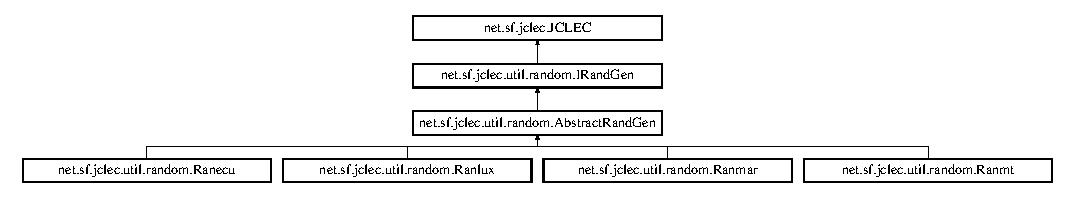
\includegraphics[height=2.231076cm]{classnet_1_1sf_1_1jclec_1_1util_1_1random_1_1_abstract_rand_gen}
\end{center}
\end{figure}
\subsection*{Public Member Functions}
\begin{DoxyCompactItemize}
\item 
void \hyperlink{classnet_1_1sf_1_1jclec_1_1util_1_1random_1_1_abstract_rand_gen_ab62c6eb80397722ae312482efdd41992}{raw} (double\mbox{[}$\,$\mbox{]} d, int n)
\item 
final void \hyperlink{classnet_1_1sf_1_1jclec_1_1util_1_1random_1_1_abstract_rand_gen_a7ab41eb7f7603618a1945bbc0d78b419}{raw} (double\mbox{[}$\,$\mbox{]} d)
\item 
final int \hyperlink{classnet_1_1sf_1_1jclec_1_1util_1_1random_1_1_abstract_rand_gen_a55c6e19b359472839a05f3813c7f2e08}{choose} (int hi)
\item 
int \hyperlink{classnet_1_1sf_1_1jclec_1_1util_1_1random_1_1_abstract_rand_gen_acf07aa5a639e6c8fdea7122de17948e3}{choose} (int lo, int hi)
\item 
final boolean \hyperlink{classnet_1_1sf_1_1jclec_1_1util_1_1random_1_1_abstract_rand_gen_a351e4fb64b629ee1778f739ab54c4c74}{coin} ()
\item 
final boolean \hyperlink{classnet_1_1sf_1_1jclec_1_1util_1_1random_1_1_abstract_rand_gen_a0b2cc6c273c2112c4f7f39c126a7b10b}{coin} (double p)
\item 
final double \hyperlink{classnet_1_1sf_1_1jclec_1_1util_1_1random_1_1_abstract_rand_gen_a24478e919b8d389d4e26b52f2532307c}{uniform} (double lo, double hi)
\item 
final double \hyperlink{classnet_1_1sf_1_1jclec_1_1util_1_1random_1_1_abstract_rand_gen_a249bd51a907c6d0f8792f2964bef7924}{gaussian} ()
\item 
final double \hyperlink{classnet_1_1sf_1_1jclec_1_1util_1_1random_1_1_abstract_rand_gen_a54c77e3e2d11e70b64ba4541c5be5f13}{gaussian} (double sd)
\item 
final double \hyperlink{classnet_1_1sf_1_1jclec_1_1util_1_1random_1_1_abstract_rand_gen_a943833520962f5db5c4a748db272dad7}{powlaw} (double alpha, double cut)
\end{DoxyCompactItemize}
\subsection*{Protected Member Functions}
\begin{DoxyCompactItemize}
\item 
\hyperlink{classnet_1_1sf_1_1jclec_1_1util_1_1random_1_1_abstract_rand_gen_af19cc77f3b73602085356ccd124c678b}{Abstract\-Rand\-Gen} ()
\end{DoxyCompactItemize}
\subsection*{Protected Attributes}
\begin{DoxyCompactItemize}
\item 
Double \hyperlink{classnet_1_1sf_1_1jclec_1_1util_1_1random_1_1_abstract_rand_gen_a3185942553b54d150bf1252fa0c03c7d}{B\-Moutput}
\end{DoxyCompactItemize}


\subsection{Detailed Description}
Base implementation of the \hyperlink{interfacenet_1_1sf_1_1jclec_1_1util_1_1random_1_1_i_rand_gen}{I\-Rand\-Gen} interface.

\begin{DoxyAuthor}{Author}
Sebastian Ventura 
\end{DoxyAuthor}


\subsection{Constructor \& Destructor Documentation}
\hypertarget{classnet_1_1sf_1_1jclec_1_1util_1_1random_1_1_abstract_rand_gen_af19cc77f3b73602085356ccd124c678b}{\index{net\-::sf\-::jclec\-::util\-::random\-::\-Abstract\-Rand\-Gen@{net\-::sf\-::jclec\-::util\-::random\-::\-Abstract\-Rand\-Gen}!Abstract\-Rand\-Gen@{Abstract\-Rand\-Gen}}
\index{Abstract\-Rand\-Gen@{Abstract\-Rand\-Gen}!net::sf::jclec::util::random::AbstractRandGen@{net\-::sf\-::jclec\-::util\-::random\-::\-Abstract\-Rand\-Gen}}
\subsubsection[{Abstract\-Rand\-Gen}]{\setlength{\rightskip}{0pt plus 5cm}net.\-sf.\-jclec.\-util.\-random.\-Abstract\-Rand\-Gen.\-Abstract\-Rand\-Gen (
\begin{DoxyParamCaption}
{}
\end{DoxyParamCaption}
)\hspace{0.3cm}{\ttfamily [protected]}}}\label{classnet_1_1sf_1_1jclec_1_1util_1_1random_1_1_abstract_rand_gen_af19cc77f3b73602085356ccd124c678b}
Empty constructor. 

\subsection{Member Function Documentation}
\hypertarget{classnet_1_1sf_1_1jclec_1_1util_1_1random_1_1_abstract_rand_gen_a55c6e19b359472839a05f3813c7f2e08}{\index{net\-::sf\-::jclec\-::util\-::random\-::\-Abstract\-Rand\-Gen@{net\-::sf\-::jclec\-::util\-::random\-::\-Abstract\-Rand\-Gen}!choose@{choose}}
\index{choose@{choose}!net::sf::jclec::util::random::AbstractRandGen@{net\-::sf\-::jclec\-::util\-::random\-::\-Abstract\-Rand\-Gen}}
\subsubsection[{choose}]{\setlength{\rightskip}{0pt plus 5cm}final int net.\-sf.\-jclec.\-util.\-random.\-Abstract\-Rand\-Gen.\-choose (
\begin{DoxyParamCaption}
\item[{int}]{hi}
\end{DoxyParamCaption}
)}}\label{classnet_1_1sf_1_1jclec_1_1util_1_1random_1_1_abstract_rand_gen_a55c6e19b359472839a05f3813c7f2e08}
Return an integer random value in the range \mbox{[}1, ...hi)


\begin{DoxyParams}{Parameters}
{\em hi} & upper limit of range.\\
\hline
\end{DoxyParams}
\begin{DoxyReturn}{Returns}
a random integer in the range.
\end{DoxyReturn}
 

Implements \hyperlink{interfacenet_1_1sf_1_1jclec_1_1util_1_1random_1_1_i_rand_gen_a98171510a2905523f08ab7cfd59ddc98}{net.\-sf.\-jclec.\-util.\-random.\-I\-Rand\-Gen}.

\hypertarget{classnet_1_1sf_1_1jclec_1_1util_1_1random_1_1_abstract_rand_gen_acf07aa5a639e6c8fdea7122de17948e3}{\index{net\-::sf\-::jclec\-::util\-::random\-::\-Abstract\-Rand\-Gen@{net\-::sf\-::jclec\-::util\-::random\-::\-Abstract\-Rand\-Gen}!choose@{choose}}
\index{choose@{choose}!net::sf::jclec::util::random::AbstractRandGen@{net\-::sf\-::jclec\-::util\-::random\-::\-Abstract\-Rand\-Gen}}
\subsubsection[{choose}]{\setlength{\rightskip}{0pt plus 5cm}int net.\-sf.\-jclec.\-util.\-random.\-Abstract\-Rand\-Gen.\-choose (
\begin{DoxyParamCaption}
\item[{int}]{lo, }
\item[{int}]{hi}
\end{DoxyParamCaption}
)}}\label{classnet_1_1sf_1_1jclec_1_1util_1_1random_1_1_abstract_rand_gen_acf07aa5a639e6c8fdea7122de17948e3}
Return an integer random value in the range \mbox{[}lo, ...hi)


\begin{DoxyParams}{Parameters}
{\em lo} & lower limit of range \\
\hline
{\em hi} & upper limit of range\\
\hline
\end{DoxyParams}
\begin{DoxyReturn}{Returns}
a random integer in the range.
\end{DoxyReturn}
 

Implements \hyperlink{interfacenet_1_1sf_1_1jclec_1_1util_1_1random_1_1_i_rand_gen_ac49d06156eeeea535792996b15f8b8a4}{net.\-sf.\-jclec.\-util.\-random.\-I\-Rand\-Gen}.

\hypertarget{classnet_1_1sf_1_1jclec_1_1util_1_1random_1_1_abstract_rand_gen_a351e4fb64b629ee1778f739ab54c4c74}{\index{net\-::sf\-::jclec\-::util\-::random\-::\-Abstract\-Rand\-Gen@{net\-::sf\-::jclec\-::util\-::random\-::\-Abstract\-Rand\-Gen}!coin@{coin}}
\index{coin@{coin}!net::sf::jclec::util::random::AbstractRandGen@{net\-::sf\-::jclec\-::util\-::random\-::\-Abstract\-Rand\-Gen}}
\subsubsection[{coin}]{\setlength{\rightskip}{0pt plus 5cm}final boolean net.\-sf.\-jclec.\-util.\-random.\-Abstract\-Rand\-Gen.\-coin (
\begin{DoxyParamCaption}
{}
\end{DoxyParamCaption}
)}}\label{classnet_1_1sf_1_1jclec_1_1util_1_1random_1_1_abstract_rand_gen_a351e4fb64b629ee1778f739ab54c4c74}
Return a boolean that's true 0.\-5 of the time. This method call is equivalent to coin(0.\-5).

\begin{DoxyReturn}{Returns}
a boolean that's true 0.\-5 of the time.
\end{DoxyReturn}
 

Implements \hyperlink{interfacenet_1_1sf_1_1jclec_1_1util_1_1random_1_1_i_rand_gen_a59c165689aeaed76946f86e780da4bb3}{net.\-sf.\-jclec.\-util.\-random.\-I\-Rand\-Gen}.

\hypertarget{classnet_1_1sf_1_1jclec_1_1util_1_1random_1_1_abstract_rand_gen_a0b2cc6c273c2112c4f7f39c126a7b10b}{\index{net\-::sf\-::jclec\-::util\-::random\-::\-Abstract\-Rand\-Gen@{net\-::sf\-::jclec\-::util\-::random\-::\-Abstract\-Rand\-Gen}!coin@{coin}}
\index{coin@{coin}!net::sf::jclec::util::random::AbstractRandGen@{net\-::sf\-::jclec\-::util\-::random\-::\-Abstract\-Rand\-Gen}}
\subsubsection[{coin}]{\setlength{\rightskip}{0pt plus 5cm}final boolean net.\-sf.\-jclec.\-util.\-random.\-Abstract\-Rand\-Gen.\-coin (
\begin{DoxyParamCaption}
\item[{double}]{p}
\end{DoxyParamCaption}
)}}\label{classnet_1_1sf_1_1jclec_1_1util_1_1random_1_1_abstract_rand_gen_a0b2cc6c273c2112c4f7f39c126a7b10b}
Return a boolean that's true p of the time.


\begin{DoxyParams}{Parameters}
{\em p} & probability that function will return true.\\
\hline
\end{DoxyParams}
\begin{DoxyReturn}{Returns}
a boolean that's true p of the time.
\end{DoxyReturn}
 

Implements \hyperlink{interfacenet_1_1sf_1_1jclec_1_1util_1_1random_1_1_i_rand_gen_a72fb48421115797f64d7eba977094d76}{net.\-sf.\-jclec.\-util.\-random.\-I\-Rand\-Gen}.

\hypertarget{classnet_1_1sf_1_1jclec_1_1util_1_1random_1_1_abstract_rand_gen_a249bd51a907c6d0f8792f2964bef7924}{\index{net\-::sf\-::jclec\-::util\-::random\-::\-Abstract\-Rand\-Gen@{net\-::sf\-::jclec\-::util\-::random\-::\-Abstract\-Rand\-Gen}!gaussian@{gaussian}}
\index{gaussian@{gaussian}!net::sf::jclec::util::random::AbstractRandGen@{net\-::sf\-::jclec\-::util\-::random\-::\-Abstract\-Rand\-Gen}}
\subsubsection[{gaussian}]{\setlength{\rightskip}{0pt plus 5cm}final double net.\-sf.\-jclec.\-util.\-random.\-Abstract\-Rand\-Gen.\-gaussian (
\begin{DoxyParamCaption}
{}
\end{DoxyParamCaption}
)}}\label{classnet_1_1sf_1_1jclec_1_1util_1_1random_1_1_abstract_rand_gen_a249bd51a907c6d0f8792f2964bef7924}
Uses the Box-\/\-Muller algorithm to transform raw's into gaussian deviates.

\begin{DoxyReturn}{Returns}
a random real with a gaussian distribution and unitary standard deviation.
\end{DoxyReturn}
 

Implements \hyperlink{interfacenet_1_1sf_1_1jclec_1_1util_1_1random_1_1_i_rand_gen_ad27d74d84372c2f39ef32466eeae655d}{net.\-sf.\-jclec.\-util.\-random.\-I\-Rand\-Gen}.

\hypertarget{classnet_1_1sf_1_1jclec_1_1util_1_1random_1_1_abstract_rand_gen_a54c77e3e2d11e70b64ba4541c5be5f13}{\index{net\-::sf\-::jclec\-::util\-::random\-::\-Abstract\-Rand\-Gen@{net\-::sf\-::jclec\-::util\-::random\-::\-Abstract\-Rand\-Gen}!gaussian@{gaussian}}
\index{gaussian@{gaussian}!net::sf::jclec::util::random::AbstractRandGen@{net\-::sf\-::jclec\-::util\-::random\-::\-Abstract\-Rand\-Gen}}
\subsubsection[{gaussian}]{\setlength{\rightskip}{0pt plus 5cm}final double net.\-sf.\-jclec.\-util.\-random.\-Abstract\-Rand\-Gen.\-gaussian (
\begin{DoxyParamCaption}
\item[{double}]{sd}
\end{DoxyParamCaption}
)}}\label{classnet_1_1sf_1_1jclec_1_1util_1_1random_1_1_abstract_rand_gen_a54c77e3e2d11e70b64ba4541c5be5f13}
Return a gaussian distributed random real value with standard deviation \char`\"{}sd\char`\"{}.


\begin{DoxyParams}{Parameters}
{\em sd} & standard deviation.\\
\hline
\end{DoxyParams}
\begin{DoxyReturn}{Returns}
a random real with gaussian distribution and standard deviation sd.
\end{DoxyReturn}
 

Implements \hyperlink{interfacenet_1_1sf_1_1jclec_1_1util_1_1random_1_1_i_rand_gen_a140ae908e5c603244d37e8095265271d}{net.\-sf.\-jclec.\-util.\-random.\-I\-Rand\-Gen}.

\hypertarget{classnet_1_1sf_1_1jclec_1_1util_1_1random_1_1_abstract_rand_gen_a943833520962f5db5c4a748db272dad7}{\index{net\-::sf\-::jclec\-::util\-::random\-::\-Abstract\-Rand\-Gen@{net\-::sf\-::jclec\-::util\-::random\-::\-Abstract\-Rand\-Gen}!powlaw@{powlaw}}
\index{powlaw@{powlaw}!net::sf::jclec::util::random::AbstractRandGen@{net\-::sf\-::jclec\-::util\-::random\-::\-Abstract\-Rand\-Gen}}
\subsubsection[{powlaw}]{\setlength{\rightskip}{0pt plus 5cm}final double net.\-sf.\-jclec.\-util.\-random.\-Abstract\-Rand\-Gen.\-powlaw (
\begin{DoxyParamCaption}
\item[{double}]{alpha, }
\item[{double}]{cut}
\end{DoxyParamCaption}
)}}\label{classnet_1_1sf_1_1jclec_1_1util_1_1random_1_1_abstract_rand_gen_a943833520962f5db5c4a748db272dad7}
Generate a \char`\"{}power-\/law  distribution\char`\"{} with exponent \char`\"{}alpha\char`\"{} and lower cutoff \char`\"{}cut\char`\"{}.


\begin{DoxyParams}{Parameters}
{\em alpha} & the exponent. \\
\hline
{\em cut} & the lower cutoff. \\
\hline
\end{DoxyParams}
 

Implements \hyperlink{interfacenet_1_1sf_1_1jclec_1_1util_1_1random_1_1_i_rand_gen_aea94f3f66f7533cdccd7f3312bd9b149}{net.\-sf.\-jclec.\-util.\-random.\-I\-Rand\-Gen}.

\hypertarget{classnet_1_1sf_1_1jclec_1_1util_1_1random_1_1_abstract_rand_gen_ab62c6eb80397722ae312482efdd41992}{\index{net\-::sf\-::jclec\-::util\-::random\-::\-Abstract\-Rand\-Gen@{net\-::sf\-::jclec\-::util\-::random\-::\-Abstract\-Rand\-Gen}!raw@{raw}}
\index{raw@{raw}!net::sf::jclec::util::random::AbstractRandGen@{net\-::sf\-::jclec\-::util\-::random\-::\-Abstract\-Rand\-Gen}}
\subsubsection[{raw}]{\setlength{\rightskip}{0pt plus 5cm}void net.\-sf.\-jclec.\-util.\-random.\-Abstract\-Rand\-Gen.\-raw (
\begin{DoxyParamCaption}
\item[{double\mbox{[}$\,$\mbox{]}}]{d, }
\item[{int}]{n}
\end{DoxyParamCaption}
)}}\label{classnet_1_1sf_1_1jclec_1_1util_1_1random_1_1_abstract_rand_gen_ab62c6eb80397722ae312482efdd41992}
Fill part or all of an array with doubles.


\begin{DoxyParams}{Parameters}
{\em d} & array to be filled with doubles. \\
\hline
{\em n} & number of doubles to generate.\\
\hline
\end{DoxyParams}
 

Implements \hyperlink{interfacenet_1_1sf_1_1jclec_1_1util_1_1random_1_1_i_rand_gen_ac30d440c578db88288430b1b8c36cace}{net.\-sf.\-jclec.\-util.\-random.\-I\-Rand\-Gen}.

\hypertarget{classnet_1_1sf_1_1jclec_1_1util_1_1random_1_1_abstract_rand_gen_a7ab41eb7f7603618a1945bbc0d78b419}{\index{net\-::sf\-::jclec\-::util\-::random\-::\-Abstract\-Rand\-Gen@{net\-::sf\-::jclec\-::util\-::random\-::\-Abstract\-Rand\-Gen}!raw@{raw}}
\index{raw@{raw}!net::sf::jclec::util::random::AbstractRandGen@{net\-::sf\-::jclec\-::util\-::random\-::\-Abstract\-Rand\-Gen}}
\subsubsection[{raw}]{\setlength{\rightskip}{0pt plus 5cm}final void net.\-sf.\-jclec.\-util.\-random.\-Abstract\-Rand\-Gen.\-raw (
\begin{DoxyParamCaption}
\item[{double\mbox{[}$\,$\mbox{]}}]{d}
\end{DoxyParamCaption}
)}}\label{classnet_1_1sf_1_1jclec_1_1util_1_1random_1_1_abstract_rand_gen_a7ab41eb7f7603618a1945bbc0d78b419}
Fill an entire array with doubles.


\begin{DoxyParams}{Parameters}
{\em d} & array to be filled with doubles.\\
\hline
\end{DoxyParams}
 

Implements \hyperlink{interfacenet_1_1sf_1_1jclec_1_1util_1_1random_1_1_i_rand_gen_a200557979a79ca8e7a0878d41099b966}{net.\-sf.\-jclec.\-util.\-random.\-I\-Rand\-Gen}.

\hypertarget{classnet_1_1sf_1_1jclec_1_1util_1_1random_1_1_abstract_rand_gen_a24478e919b8d389d4e26b52f2532307c}{\index{net\-::sf\-::jclec\-::util\-::random\-::\-Abstract\-Rand\-Gen@{net\-::sf\-::jclec\-::util\-::random\-::\-Abstract\-Rand\-Gen}!uniform@{uniform}}
\index{uniform@{uniform}!net::sf::jclec::util::random::AbstractRandGen@{net\-::sf\-::jclec\-::util\-::random\-::\-Abstract\-Rand\-Gen}}
\subsubsection[{uniform}]{\setlength{\rightskip}{0pt plus 5cm}final double net.\-sf.\-jclec.\-util.\-random.\-Abstract\-Rand\-Gen.\-uniform (
\begin{DoxyParamCaption}
\item[{double}]{lo, }
\item[{double}]{hi}
\end{DoxyParamCaption}
)}}\label{classnet_1_1sf_1_1jclec_1_1util_1_1random_1_1_abstract_rand_gen_a24478e919b8d389d4e26b52f2532307c}
Return a uniform random real in the range \mbox{[}lo, hi\mbox{]}.


\begin{DoxyParams}{Parameters}
{\em lo} & lower limit of range. \\
\hline
{\em hi} & upper limit of range.\\
\hline
\end{DoxyParams}
\begin{DoxyReturn}{Returns}
a uniform random real in the range.
\end{DoxyReturn}
 

Implements \hyperlink{interfacenet_1_1sf_1_1jclec_1_1util_1_1random_1_1_i_rand_gen_a03e4b879098129fd153ee8590fb2c98a}{net.\-sf.\-jclec.\-util.\-random.\-I\-Rand\-Gen}.



\subsection{Member Data Documentation}
\hypertarget{classnet_1_1sf_1_1jclec_1_1util_1_1random_1_1_abstract_rand_gen_a3185942553b54d150bf1252fa0c03c7d}{\index{net\-::sf\-::jclec\-::util\-::random\-::\-Abstract\-Rand\-Gen@{net\-::sf\-::jclec\-::util\-::random\-::\-Abstract\-Rand\-Gen}!B\-Moutput@{B\-Moutput}}
\index{B\-Moutput@{B\-Moutput}!net::sf::jclec::util::random::AbstractRandGen@{net\-::sf\-::jclec\-::util\-::random\-::\-Abstract\-Rand\-Gen}}
\subsubsection[{B\-Moutput}]{\setlength{\rightskip}{0pt plus 5cm}Double net.\-sf.\-jclec.\-util.\-random.\-Abstract\-Rand\-Gen.\-B\-Moutput\hspace{0.3cm}{\ttfamily [protected]}}}\label{classnet_1_1sf_1_1jclec_1_1util_1_1random_1_1_abstract_rand_gen_a3185942553b54d150bf1252fa0c03c7d}
Constant used in the Box-\/\-Mueller algorithm. 

The documentation for this class was generated from the following file\-:\begin{DoxyCompactItemize}
\item 
src/main/java/net/sf/jclec/util/random/Abstract\-Rand\-Gen.\-java\end{DoxyCompactItemize}

\hypertarget{classnet_1_1sf_1_1jclec_1_1util_1_1random_1_1_abstract_rand_gen_factory}{\section{net.\-sf.\-jclec.\-util.\-random.\-Abstract\-Rand\-Gen\-Factory Class Reference}
\label{classnet_1_1sf_1_1jclec_1_1util_1_1random_1_1_abstract_rand_gen_factory}\index{net.\-sf.\-jclec.\-util.\-random.\-Abstract\-Rand\-Gen\-Factory@{net.\-sf.\-jclec.\-util.\-random.\-Abstract\-Rand\-Gen\-Factory}}
}
Inheritance diagram for net.\-sf.\-jclec.\-util.\-random.\-Abstract\-Rand\-Gen\-Factory\-:\begin{figure}[H]
\begin{center}
\leavevmode
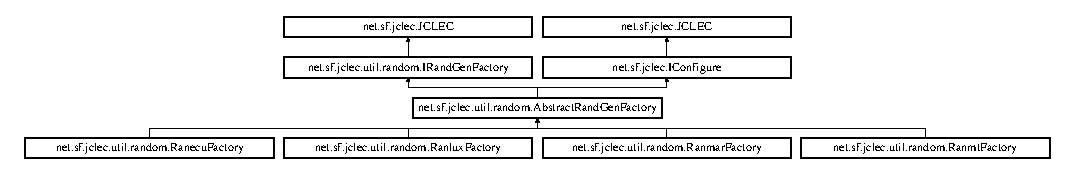
\includegraphics[height=1.898305cm]{classnet_1_1sf_1_1jclec_1_1util_1_1random_1_1_abstract_rand_gen_factory}
\end{center}
\end{figure}
\subsection*{Public Member Functions}
\begin{DoxyCompactItemize}
\item 
\hyperlink{classnet_1_1sf_1_1jclec_1_1util_1_1random_1_1_abstract_rand_gen_factory_a951485e5b8b752b7bf3c11558238e25b}{Abstract\-Rand\-Gen\-Factory} ()
\item 
int \hyperlink{classnet_1_1sf_1_1jclec_1_1util_1_1random_1_1_abstract_rand_gen_factory_a7079e322cbf8af86411018419fa4258f}{get\-Seed} ()
\item 
void \hyperlink{classnet_1_1sf_1_1jclec_1_1util_1_1random_1_1_abstract_rand_gen_factory_ac87c545525657b0dee889c52c42ce58d}{set\-Seed} (int seed)
\item 
void \hyperlink{classnet_1_1sf_1_1jclec_1_1util_1_1random_1_1_abstract_rand_gen_factory_adbcc614c5ec7ae7d3a161286f2e5f741}{configure} (Configuration settings)
\end{DoxyCompactItemize}
\subsection*{Protected Attributes}
\begin{DoxyCompactItemize}
\item 
\hyperlink{classnet_1_1sf_1_1jclec_1_1util_1_1random_1_1_seed_generator}{Seed\-Generator} \hyperlink{classnet_1_1sf_1_1jclec_1_1util_1_1random_1_1_abstract_rand_gen_factory_ae3ca4d4c2dd0f8b276b2ef5d9725dae8}{seed\-Generator} = new \hyperlink{classnet_1_1sf_1_1jclec_1_1util_1_1random_1_1_seed_generator}{Seed\-Generator}()
\end{DoxyCompactItemize}


\subsection{Detailed Description}
\hyperlink{interfacenet_1_1sf_1_1jclec_1_1util_1_1random_1_1_i_rand_gen_factory}{I\-Rand\-Gen\-Factory} abstract implementation...

\begin{DoxyAuthor}{Author}
Sebastian Ventura 
\end{DoxyAuthor}


\subsection{Constructor \& Destructor Documentation}
\hypertarget{classnet_1_1sf_1_1jclec_1_1util_1_1random_1_1_abstract_rand_gen_factory_a951485e5b8b752b7bf3c11558238e25b}{\index{net\-::sf\-::jclec\-::util\-::random\-::\-Abstract\-Rand\-Gen\-Factory@{net\-::sf\-::jclec\-::util\-::random\-::\-Abstract\-Rand\-Gen\-Factory}!Abstract\-Rand\-Gen\-Factory@{Abstract\-Rand\-Gen\-Factory}}
\index{Abstract\-Rand\-Gen\-Factory@{Abstract\-Rand\-Gen\-Factory}!net::sf::jclec::util::random::AbstractRandGenFactory@{net\-::sf\-::jclec\-::util\-::random\-::\-Abstract\-Rand\-Gen\-Factory}}
\subsubsection[{Abstract\-Rand\-Gen\-Factory}]{\setlength{\rightskip}{0pt plus 5cm}net.\-sf.\-jclec.\-util.\-random.\-Abstract\-Rand\-Gen\-Factory.\-Abstract\-Rand\-Gen\-Factory (
\begin{DoxyParamCaption}
{}
\end{DoxyParamCaption}
)}}\label{classnet_1_1sf_1_1jclec_1_1util_1_1random_1_1_abstract_rand_gen_factory_a951485e5b8b752b7bf3c11558238e25b}
Empty (default) constructor 

\subsection{Member Function Documentation}
\hypertarget{classnet_1_1sf_1_1jclec_1_1util_1_1random_1_1_abstract_rand_gen_factory_adbcc614c5ec7ae7d3a161286f2e5f741}{\index{net\-::sf\-::jclec\-::util\-::random\-::\-Abstract\-Rand\-Gen\-Factory@{net\-::sf\-::jclec\-::util\-::random\-::\-Abstract\-Rand\-Gen\-Factory}!configure@{configure}}
\index{configure@{configure}!net::sf::jclec::util::random::AbstractRandGenFactory@{net\-::sf\-::jclec\-::util\-::random\-::\-Abstract\-Rand\-Gen\-Factory}}
\subsubsection[{configure}]{\setlength{\rightskip}{0pt plus 5cm}void net.\-sf.\-jclec.\-util.\-random.\-Abstract\-Rand\-Gen\-Factory.\-configure (
\begin{DoxyParamCaption}
\item[{Configuration}]{settings}
\end{DoxyParamCaption}
)}}\label{classnet_1_1sf_1_1jclec_1_1util_1_1random_1_1_abstract_rand_gen_factory_adbcc614c5ec7ae7d3a161286f2e5f741}
Configuration method.

Configuration parameters for this object are...


\begin{DoxyParams}{Parameters}
{\em settings} & Configuration settings \\
\hline
\end{DoxyParams}


Implements \hyperlink{interfacenet_1_1sf_1_1jclec_1_1_i_configure_add31a65a04d148c690a956fbbad6987c}{net.\-sf.\-jclec.\-I\-Configure}.

\hypertarget{classnet_1_1sf_1_1jclec_1_1util_1_1random_1_1_abstract_rand_gen_factory_a7079e322cbf8af86411018419fa4258f}{\index{net\-::sf\-::jclec\-::util\-::random\-::\-Abstract\-Rand\-Gen\-Factory@{net\-::sf\-::jclec\-::util\-::random\-::\-Abstract\-Rand\-Gen\-Factory}!get\-Seed@{get\-Seed}}
\index{get\-Seed@{get\-Seed}!net::sf::jclec::util::random::AbstractRandGenFactory@{net\-::sf\-::jclec\-::util\-::random\-::\-Abstract\-Rand\-Gen\-Factory}}
\subsubsection[{get\-Seed}]{\setlength{\rightskip}{0pt plus 5cm}int net.\-sf.\-jclec.\-util.\-random.\-Abstract\-Rand\-Gen\-Factory.\-get\-Seed (
\begin{DoxyParamCaption}
{}
\end{DoxyParamCaption}
)}}\label{classnet_1_1sf_1_1jclec_1_1util_1_1random_1_1_abstract_rand_gen_factory_a7079e322cbf8af86411018419fa4258f}
Access to actual generators seed.

\begin{DoxyReturn}{Returns}
Actual generators seed 
\end{DoxyReturn}
\hypertarget{classnet_1_1sf_1_1jclec_1_1util_1_1random_1_1_abstract_rand_gen_factory_ac87c545525657b0dee889c52c42ce58d}{\index{net\-::sf\-::jclec\-::util\-::random\-::\-Abstract\-Rand\-Gen\-Factory@{net\-::sf\-::jclec\-::util\-::random\-::\-Abstract\-Rand\-Gen\-Factory}!set\-Seed@{set\-Seed}}
\index{set\-Seed@{set\-Seed}!net::sf::jclec::util::random::AbstractRandGenFactory@{net\-::sf\-::jclec\-::util\-::random\-::\-Abstract\-Rand\-Gen\-Factory}}
\subsubsection[{set\-Seed}]{\setlength{\rightskip}{0pt plus 5cm}void net.\-sf.\-jclec.\-util.\-random.\-Abstract\-Rand\-Gen\-Factory.\-set\-Seed (
\begin{DoxyParamCaption}
\item[{int}]{seed}
\end{DoxyParamCaption}
)}}\label{classnet_1_1sf_1_1jclec_1_1util_1_1random_1_1_abstract_rand_gen_factory_ac87c545525657b0dee889c52c42ce58d}
Sets actual generators seed.


\begin{DoxyParams}{Parameters}
{\em seed} & New generators seed \\
\hline
\end{DoxyParams}


\subsection{Member Data Documentation}
\hypertarget{classnet_1_1sf_1_1jclec_1_1util_1_1random_1_1_abstract_rand_gen_factory_ae3ca4d4c2dd0f8b276b2ef5d9725dae8}{\index{net\-::sf\-::jclec\-::util\-::random\-::\-Abstract\-Rand\-Gen\-Factory@{net\-::sf\-::jclec\-::util\-::random\-::\-Abstract\-Rand\-Gen\-Factory}!seed\-Generator@{seed\-Generator}}
\index{seed\-Generator@{seed\-Generator}!net::sf::jclec::util::random::AbstractRandGenFactory@{net\-::sf\-::jclec\-::util\-::random\-::\-Abstract\-Rand\-Gen\-Factory}}
\subsubsection[{seed\-Generator}]{\setlength{\rightskip}{0pt plus 5cm}{\bf Seed\-Generator} net.\-sf.\-jclec.\-util.\-random.\-Abstract\-Rand\-Gen\-Factory.\-seed\-Generator = new {\bf Seed\-Generator}()\hspace{0.3cm}{\ttfamily [protected]}}}\label{classnet_1_1sf_1_1jclec_1_1util_1_1random_1_1_abstract_rand_gen_factory_ae3ca4d4c2dd0f8b276b2ef5d9725dae8}
Seeds generator 

The documentation for this class was generated from the following file\-:\begin{DoxyCompactItemize}
\item 
src/main/java/net/sf/jclec/util/random/Abstract\-Rand\-Gen\-Factory.\-java\end{DoxyCompactItemize}

\hypertarget{classnet_1_1sf_1_1jclec_1_1base_1_1_abstract_recombinator}{\section{net.\-sf.\-jclec.\-base.\-Abstract\-Recombinator Class Reference}
\label{classnet_1_1sf_1_1jclec_1_1base_1_1_abstract_recombinator}\index{net.\-sf.\-jclec.\-base.\-Abstract\-Recombinator@{net.\-sf.\-jclec.\-base.\-Abstract\-Recombinator}}
}
Inheritance diagram for net.\-sf.\-jclec.\-base.\-Abstract\-Recombinator\-:\begin{figure}[H]
\begin{center}
\leavevmode
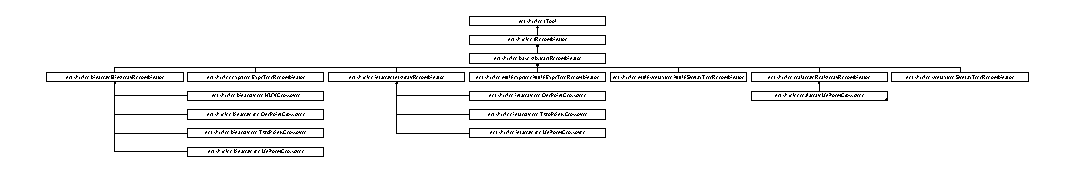
\includegraphics[height=1.876833cm]{classnet_1_1sf_1_1jclec_1_1base_1_1_abstract_recombinator}
\end{center}
\end{figure}
\subsection*{Public Member Functions}
\begin{DoxyCompactItemize}
\item 
\hyperlink{classnet_1_1sf_1_1jclec_1_1base_1_1_abstract_recombinator_ae14b57d058c733a0b53244135e20f8f6}{Abstract\-Recombinator} ()
\item 
final void \hyperlink{classnet_1_1sf_1_1jclec_1_1base_1_1_abstract_recombinator_aa07502c99a8d181ac13d69d464bbd703}{contextualize} (\hyperlink{interfacenet_1_1sf_1_1jclec_1_1_i_system}{I\-System} \hyperlink{classnet_1_1sf_1_1jclec_1_1base_1_1_abstract_recombinator_a580de9e9511dbb1d9042eb1089e767a7}{context})
\item 
final int \hyperlink{classnet_1_1sf_1_1jclec_1_1base_1_1_abstract_recombinator_aacb99468526b391800cca57f1f8a5df3}{get\-Ppl} ()
\item 
final int \hyperlink{classnet_1_1sf_1_1jclec_1_1base_1_1_abstract_recombinator_a36463c68ebe030a7ff428fe81611ca80}{get\-Spl} ()
\item 
List$<$ \hyperlink{interfacenet_1_1sf_1_1jclec_1_1_i_individual}{I\-Individual} $>$ \hyperlink{classnet_1_1sf_1_1jclec_1_1base_1_1_abstract_recombinator_a5f4024acbf65e43bdfa7844dc23731cd}{recombine} (List$<$ \hyperlink{interfacenet_1_1sf_1_1jclec_1_1_i_individual}{I\-Individual} $>$ parents)
\end{DoxyCompactItemize}
\subsection*{Protected Member Functions}
\begin{DoxyCompactItemize}
\item 
abstract void \hyperlink{classnet_1_1sf_1_1jclec_1_1base_1_1_abstract_recombinator_aa90f858c27f9da69b2f7bb0a9220ed4e}{set\-Ppl} ()
\item 
abstract void \hyperlink{classnet_1_1sf_1_1jclec_1_1base_1_1_abstract_recombinator_a49a445f27d777d6f439d97d61f2e1729}{set\-Spl} ()
\item 
abstract void \hyperlink{classnet_1_1sf_1_1jclec_1_1base_1_1_abstract_recombinator_ad9518cc41f28166465c4b8dc60059048}{prepare\-Recombination} ()
\item 
abstract void \hyperlink{classnet_1_1sf_1_1jclec_1_1base_1_1_abstract_recombinator_a1f94790294ad036473b5e1ffa563597e}{recombine\-Next} ()
\end{DoxyCompactItemize}
\subsection*{Protected Attributes}
\begin{DoxyCompactItemize}
\item 
\hyperlink{interfacenet_1_1sf_1_1jclec_1_1_i_population}{I\-Population} \hyperlink{classnet_1_1sf_1_1jclec_1_1base_1_1_abstract_recombinator_a580de9e9511dbb1d9042eb1089e767a7}{context}
\item 
\hyperlink{interfacenet_1_1sf_1_1jclec_1_1util_1_1random_1_1_i_rand_gen}{I\-Rand\-Gen} \hyperlink{classnet_1_1sf_1_1jclec_1_1base_1_1_abstract_recombinator_a423dad16f0b307358eb263da316de7a5}{randgen}
\item 
transient int \hyperlink{classnet_1_1sf_1_1jclec_1_1base_1_1_abstract_recombinator_a28f82e20ff940f4ebbe2be58a64adf0a}{ppl}
\item 
transient int \hyperlink{classnet_1_1sf_1_1jclec_1_1base_1_1_abstract_recombinator_acc9ceca89a1680db0a6ec818c1ac2a67}{spl}
\item 
transient List$<$ \hyperlink{interfacenet_1_1sf_1_1jclec_1_1_i_individual}{I\-Individual} $>$ \hyperlink{classnet_1_1sf_1_1jclec_1_1base_1_1_abstract_recombinator_a47b6dacf54a78391075736cc51caf7d1}{parents\-Buffer}
\item 
transient List$<$ \hyperlink{interfacenet_1_1sf_1_1jclec_1_1_i_individual}{I\-Individual} $>$ \hyperlink{classnet_1_1sf_1_1jclec_1_1base_1_1_abstract_recombinator_a8faa0eff785de5bad8b2db01170e6f2e}{sons\-Buffer}
\item 
transient int \hyperlink{classnet_1_1sf_1_1jclec_1_1base_1_1_abstract_recombinator_acfce486c594e8b7e61c304ba7aba00b1}{parents\-Counter}
\end{DoxyCompactItemize}


\subsection{Detailed Description}
\hyperlink{interfacenet_1_1sf_1_1jclec_1_1_i_recombinator}{I\-Recombinator} abstract implementation.

\begin{DoxyAuthor}{Author}
Sebastian Ventura 
\end{DoxyAuthor}


\subsection{Constructor \& Destructor Documentation}
\hypertarget{classnet_1_1sf_1_1jclec_1_1base_1_1_abstract_recombinator_ae14b57d058c733a0b53244135e20f8f6}{\index{net\-::sf\-::jclec\-::base\-::\-Abstract\-Recombinator@{net\-::sf\-::jclec\-::base\-::\-Abstract\-Recombinator}!Abstract\-Recombinator@{Abstract\-Recombinator}}
\index{Abstract\-Recombinator@{Abstract\-Recombinator}!net::sf::jclec::base::AbstractRecombinator@{net\-::sf\-::jclec\-::base\-::\-Abstract\-Recombinator}}
\subsubsection[{Abstract\-Recombinator}]{\setlength{\rightskip}{0pt plus 5cm}net.\-sf.\-jclec.\-base.\-Abstract\-Recombinator.\-Abstract\-Recombinator (
\begin{DoxyParamCaption}
{}
\end{DoxyParamCaption}
)}}\label{classnet_1_1sf_1_1jclec_1_1base_1_1_abstract_recombinator_ae14b57d058c733a0b53244135e20f8f6}
Empty constructor. 

\subsection{Member Function Documentation}
\hypertarget{classnet_1_1sf_1_1jclec_1_1base_1_1_abstract_recombinator_aa07502c99a8d181ac13d69d464bbd703}{\index{net\-::sf\-::jclec\-::base\-::\-Abstract\-Recombinator@{net\-::sf\-::jclec\-::base\-::\-Abstract\-Recombinator}!contextualize@{contextualize}}
\index{contextualize@{contextualize}!net::sf::jclec::base::AbstractRecombinator@{net\-::sf\-::jclec\-::base\-::\-Abstract\-Recombinator}}
\subsubsection[{contextualize}]{\setlength{\rightskip}{0pt plus 5cm}final void net.\-sf.\-jclec.\-base.\-Abstract\-Recombinator.\-contextualize (
\begin{DoxyParamCaption}
\item[{{\bf I\-System}}]{context}
\end{DoxyParamCaption}
)}}\label{classnet_1_1sf_1_1jclec_1_1base_1_1_abstract_recombinator_aa07502c99a8d181ac13d69d464bbd703}
Set the system where ...


\begin{DoxyParams}{Parameters}
{\em context} & Execution context\\
\hline
\end{DoxyParams}
 

Implements \hyperlink{interfacenet_1_1sf_1_1jclec_1_1_i_tool_aa11b3e046b7f38e40eb4f8c72a9a2102}{net.\-sf.\-jclec.\-I\-Tool}.

\hypertarget{classnet_1_1sf_1_1jclec_1_1base_1_1_abstract_recombinator_aacb99468526b391800cca57f1f8a5df3}{\index{net\-::sf\-::jclec\-::base\-::\-Abstract\-Recombinator@{net\-::sf\-::jclec\-::base\-::\-Abstract\-Recombinator}!get\-Ppl@{get\-Ppl}}
\index{get\-Ppl@{get\-Ppl}!net::sf::jclec::base::AbstractRecombinator@{net\-::sf\-::jclec\-::base\-::\-Abstract\-Recombinator}}
\subsubsection[{get\-Ppl}]{\setlength{\rightskip}{0pt plus 5cm}final int net.\-sf.\-jclec.\-base.\-Abstract\-Recombinator.\-get\-Ppl (
\begin{DoxyParamCaption}
{}
\end{DoxyParamCaption}
)}}\label{classnet_1_1sf_1_1jclec_1_1base_1_1_abstract_recombinator_aacb99468526b391800cca57f1f8a5df3}
\begin{DoxyReturn}{Returns}
Number of parents per litter. 
\end{DoxyReturn}


Implements \hyperlink{interfacenet_1_1sf_1_1jclec_1_1_i_recombinator_a5e9e851fc35894e4e5a53531616ed42c}{net.\-sf.\-jclec.\-I\-Recombinator}.

\hypertarget{classnet_1_1sf_1_1jclec_1_1base_1_1_abstract_recombinator_a36463c68ebe030a7ff428fe81611ca80}{\index{net\-::sf\-::jclec\-::base\-::\-Abstract\-Recombinator@{net\-::sf\-::jclec\-::base\-::\-Abstract\-Recombinator}!get\-Spl@{get\-Spl}}
\index{get\-Spl@{get\-Spl}!net::sf::jclec::base::AbstractRecombinator@{net\-::sf\-::jclec\-::base\-::\-Abstract\-Recombinator}}
\subsubsection[{get\-Spl}]{\setlength{\rightskip}{0pt plus 5cm}final int net.\-sf.\-jclec.\-base.\-Abstract\-Recombinator.\-get\-Spl (
\begin{DoxyParamCaption}
{}
\end{DoxyParamCaption}
)}}\label{classnet_1_1sf_1_1jclec_1_1base_1_1_abstract_recombinator_a36463c68ebe030a7ff428fe81611ca80}
\begin{DoxyReturn}{Returns}
Number of sons per litter. 
\end{DoxyReturn}


Implements \hyperlink{interfacenet_1_1sf_1_1jclec_1_1_i_recombinator_a398927d69f307ecf449ac93c9e025933}{net.\-sf.\-jclec.\-I\-Recombinator}.

\hypertarget{classnet_1_1sf_1_1jclec_1_1base_1_1_abstract_recombinator_ad9518cc41f28166465c4b8dc60059048}{\index{net\-::sf\-::jclec\-::base\-::\-Abstract\-Recombinator@{net\-::sf\-::jclec\-::base\-::\-Abstract\-Recombinator}!prepare\-Recombination@{prepare\-Recombination}}
\index{prepare\-Recombination@{prepare\-Recombination}!net::sf::jclec::base::AbstractRecombinator@{net\-::sf\-::jclec\-::base\-::\-Abstract\-Recombinator}}
\subsubsection[{prepare\-Recombination}]{\setlength{\rightskip}{0pt plus 5cm}abstract void net.\-sf.\-jclec.\-base.\-Abstract\-Recombinator.\-prepare\-Recombination (
\begin{DoxyParamCaption}
{}
\end{DoxyParamCaption}
)\hspace{0.3cm}{\ttfamily [protected]}, {\ttfamily [pure virtual]}}}\label{classnet_1_1sf_1_1jclec_1_1base_1_1_abstract_recombinator_ad9518cc41f28166465c4b8dc60059048}
Prepare recombination process. 

Implemented in \hyperlink{classnet_1_1sf_1_1jclec_1_1multiexprtree_1_1_multi_expr_tree_recombinator_ad080cb3d90d8144a88809a308a7157cf}{net.\-sf.\-jclec.\-multiexprtree.\-Multi\-Expr\-Tree\-Recombinator}, \hyperlink{classnet_1_1sf_1_1jclec_1_1multisyntaxtree_1_1_multi_syntax_tree_recombinator_ad3ba0fcbbd052ec166f1ae11d1d8fa62}{net.\-sf.\-jclec.\-multisyntaxtree.\-Multi\-Syntax\-Tree\-Recombinator}, \hyperlink{classnet_1_1sf_1_1jclec_1_1exprtree_1_1_expr_tree_recombinator_a19632d02d287f5e08768c824695df2ac}{net.\-sf.\-jclec.\-exprtree.\-Expr\-Tree\-Recombinator}, \hyperlink{classnet_1_1sf_1_1jclec_1_1syntaxtree_1_1_syntax_tree_recombinator_acdf452d49c571862c1b660f15b62d9bd}{net.\-sf.\-jclec.\-syntaxtree.\-Syntax\-Tree\-Recombinator}, \hyperlink{classnet_1_1sf_1_1jclec_1_1intarray_1_1_int_array_recombinator_a717ae2d9111d2fb9bd98fceaf0546a99}{net.\-sf.\-jclec.\-intarray.\-Int\-Array\-Recombinator}, \hyperlink{classnet_1_1sf_1_1jclec_1_1binarray_1_1_bin_array_recombinator_adfb02ddf2e1aa3a0f3d59229f3b4334b}{net.\-sf.\-jclec.\-binarray.\-Bin\-Array\-Recombinator}, and \hyperlink{classnet_1_1sf_1_1jclec_1_1realarray_1_1_real_array_recombinator_a003b9f2418aaeab559017b9e8385bd46}{net.\-sf.\-jclec.\-realarray.\-Real\-Array\-Recombinator}.

\hypertarget{classnet_1_1sf_1_1jclec_1_1base_1_1_abstract_recombinator_a5f4024acbf65e43bdfa7844dc23731cd}{\index{net\-::sf\-::jclec\-::base\-::\-Abstract\-Recombinator@{net\-::sf\-::jclec\-::base\-::\-Abstract\-Recombinator}!recombine@{recombine}}
\index{recombine@{recombine}!net::sf::jclec::base::AbstractRecombinator@{net\-::sf\-::jclec\-::base\-::\-Abstract\-Recombinator}}
\subsubsection[{recombine}]{\setlength{\rightskip}{0pt plus 5cm}List$<${\bf I\-Individual}$>$ net.\-sf.\-jclec.\-base.\-Abstract\-Recombinator.\-recombine (
\begin{DoxyParamCaption}
\item[{List$<$ {\bf I\-Individual} $>$}]{parents}
\end{DoxyParamCaption}
)}}\label{classnet_1_1sf_1_1jclec_1_1base_1_1_abstract_recombinator_a5f4024acbf65e43bdfa7844dc23731cd}
Recombination method.


\begin{DoxyParams}{Parameters}
{\em parents} & Individuals to recombine\\
\hline
\end{DoxyParams}
\begin{DoxyReturn}{Returns}
Recombination result
\end{DoxyReturn}
 

Implements \hyperlink{interfacenet_1_1sf_1_1jclec_1_1_i_recombinator_a07721bb7be250aeae6a85e81c527e7a5}{net.\-sf.\-jclec.\-I\-Recombinator}.

\hypertarget{classnet_1_1sf_1_1jclec_1_1base_1_1_abstract_recombinator_a1f94790294ad036473b5e1ffa563597e}{\index{net\-::sf\-::jclec\-::base\-::\-Abstract\-Recombinator@{net\-::sf\-::jclec\-::base\-::\-Abstract\-Recombinator}!recombine\-Next@{recombine\-Next}}
\index{recombine\-Next@{recombine\-Next}!net::sf::jclec::base::AbstractRecombinator@{net\-::sf\-::jclec\-::base\-::\-Abstract\-Recombinator}}
\subsubsection[{recombine\-Next}]{\setlength{\rightskip}{0pt plus 5cm}abstract void net.\-sf.\-jclec.\-base.\-Abstract\-Recombinator.\-recombine\-Next (
\begin{DoxyParamCaption}
{}
\end{DoxyParamCaption}
)\hspace{0.3cm}{\ttfamily [protected]}, {\ttfamily [pure virtual]}}}\label{classnet_1_1sf_1_1jclec_1_1base_1_1_abstract_recombinator_a1f94790294ad036473b5e1ffa563597e}
Atomic recombination method. This method ... 

Implemented in \hyperlink{classnet_1_1sf_1_1jclec_1_1multiexprtree_1_1_multi_expr_tree_recombinator_a2b32688791c7f1669a5a3dfe5b440b51}{net.\-sf.\-jclec.\-multiexprtree.\-Multi\-Expr\-Tree\-Recombinator}, \hyperlink{classnet_1_1sf_1_1jclec_1_1multisyntaxtree_1_1_multi_syntax_tree_recombinator_aa9a6b30a296025db8ed66df1770017a8}{net.\-sf.\-jclec.\-multisyntaxtree.\-Multi\-Syntax\-Tree\-Recombinator}, \hyperlink{classnet_1_1sf_1_1jclec_1_1binarray_1_1rec_1_1_uniform_crossover_a99715bc9dc84ac4694ee73f1c6789242}{net.\-sf.\-jclec.\-binarray.\-rec.\-Uniform\-Crossover}, \hyperlink{classnet_1_1sf_1_1jclec_1_1exprtree_1_1_expr_tree_recombinator_adf91b5652ebb30517f565948828adfab}{net.\-sf.\-jclec.\-exprtree.\-Expr\-Tree\-Recombinator}, \hyperlink{classnet_1_1sf_1_1jclec_1_1syntaxtree_1_1_syntax_tree_recombinator_ae0f7eb381147988518b111754644aa00}{net.\-sf.\-jclec.\-syntaxtree.\-Syntax\-Tree\-Recombinator}, \hyperlink{classnet_1_1sf_1_1jclec_1_1intarray_1_1rec_1_1_uniform_crossover_a497ea31c7864b8fa7a8a3db876ff9cbd}{net.\-sf.\-jclec.\-intarray.\-rec.\-Uniform\-Crossover}, \hyperlink{classnet_1_1sf_1_1jclec_1_1realarray_1_1rec_1_1_linear_crossover_a384fc6ed44b1504cd35dca0a3497a129}{net.\-sf.\-jclec.\-realarray.\-rec.\-Linear\-Crossover}, \hyperlink{classnet_1_1sf_1_1jclec_1_1binarray_1_1rec_1_1_one_point_crossover_a37d66cb3130d54b9b95c1316de4d4b31}{net.\-sf.\-jclec.\-binarray.\-rec.\-One\-Point\-Crossover}, \hyperlink{classnet_1_1sf_1_1jclec_1_1binarray_1_1rec_1_1_two_points_crossover_a6a9d4433f97cc1b01f4030e0aa8bae63}{net.\-sf.\-jclec.\-binarray.\-rec.\-Two\-Points\-Crossover}, \hyperlink{classnet_1_1sf_1_1jclec_1_1intarray_1_1rec_1_1_one_point_crossover_a1fb4e33b91c4392c0d9a791565f4e500}{net.\-sf.\-jclec.\-intarray.\-rec.\-One\-Point\-Crossover}, \hyperlink{classnet_1_1sf_1_1jclec_1_1intarray_1_1rec_1_1_two_points_crossover_a29ac2c3118a586d806d638dfcfffd3f6}{net.\-sf.\-jclec.\-intarray.\-rec.\-Two\-Points\-Crossover}, and \hyperlink{classnet_1_1sf_1_1jclec_1_1binarray_1_1rec_1_1_h_u_x_crossover_af08ed17b50df7176acdddd4961f73ff6}{net.\-sf.\-jclec.\-binarray.\-rec.\-H\-U\-X\-Crossover}.

\hypertarget{classnet_1_1sf_1_1jclec_1_1base_1_1_abstract_recombinator_aa90f858c27f9da69b2f7bb0a9220ed4e}{\index{net\-::sf\-::jclec\-::base\-::\-Abstract\-Recombinator@{net\-::sf\-::jclec\-::base\-::\-Abstract\-Recombinator}!set\-Ppl@{set\-Ppl}}
\index{set\-Ppl@{set\-Ppl}!net::sf::jclec::base::AbstractRecombinator@{net\-::sf\-::jclec\-::base\-::\-Abstract\-Recombinator}}
\subsubsection[{set\-Ppl}]{\setlength{\rightskip}{0pt plus 5cm}abstract void net.\-sf.\-jclec.\-base.\-Abstract\-Recombinator.\-set\-Ppl (
\begin{DoxyParamCaption}
{}
\end{DoxyParamCaption}
)\hspace{0.3cm}{\ttfamily [protected]}, {\ttfamily [pure virtual]}}}\label{classnet_1_1sf_1_1jclec_1_1base_1_1_abstract_recombinator_aa90f858c27f9da69b2f7bb0a9220ed4e}
Sets the ppl parameter (that represents the number of parents per litter). 

Implemented in \hyperlink{classnet_1_1sf_1_1jclec_1_1multiexprtree_1_1_multi_expr_tree_recombinator_a98be6bca45d872a9e2aaa9b69213464b}{net.\-sf.\-jclec.\-multiexprtree.\-Multi\-Expr\-Tree\-Recombinator}, \hyperlink{classnet_1_1sf_1_1jclec_1_1multisyntaxtree_1_1_multi_syntax_tree_recombinator_a14b79cf615140c1496936dd754a773f1}{net.\-sf.\-jclec.\-multisyntaxtree.\-Multi\-Syntax\-Tree\-Recombinator}, \hyperlink{classnet_1_1sf_1_1jclec_1_1exprtree_1_1_expr_tree_recombinator_aa093b329ea2bb0c113b5b8c48107452b}{net.\-sf.\-jclec.\-exprtree.\-Expr\-Tree\-Recombinator}, \hyperlink{classnet_1_1sf_1_1jclec_1_1syntaxtree_1_1_syntax_tree_recombinator_aaa13f75a8e4aeb90b5e0637c6ed76d1d}{net.\-sf.\-jclec.\-syntaxtree.\-Syntax\-Tree\-Recombinator}, \hyperlink{classnet_1_1sf_1_1jclec_1_1realarray_1_1rec_1_1_linear_crossover_a86b0311d3a1f887602490924c0c022ce}{net.\-sf.\-jclec.\-realarray.\-rec.\-Linear\-Crossover}, \hyperlink{classnet_1_1sf_1_1jclec_1_1intarray_1_1_int_array_recombinator_a12ec5d6552bde26c176f44c96c0c5621}{net.\-sf.\-jclec.\-intarray.\-Int\-Array\-Recombinator}, and \hyperlink{classnet_1_1sf_1_1jclec_1_1binarray_1_1_bin_array_recombinator_a8ecb2813d8dca18e20c7673d94efc315}{net.\-sf.\-jclec.\-binarray.\-Bin\-Array\-Recombinator}.

\hypertarget{classnet_1_1sf_1_1jclec_1_1base_1_1_abstract_recombinator_a49a445f27d777d6f439d97d61f2e1729}{\index{net\-::sf\-::jclec\-::base\-::\-Abstract\-Recombinator@{net\-::sf\-::jclec\-::base\-::\-Abstract\-Recombinator}!set\-Spl@{set\-Spl}}
\index{set\-Spl@{set\-Spl}!net::sf::jclec::base::AbstractRecombinator@{net\-::sf\-::jclec\-::base\-::\-Abstract\-Recombinator}}
\subsubsection[{set\-Spl}]{\setlength{\rightskip}{0pt plus 5cm}abstract void net.\-sf.\-jclec.\-base.\-Abstract\-Recombinator.\-set\-Spl (
\begin{DoxyParamCaption}
{}
\end{DoxyParamCaption}
)\hspace{0.3cm}{\ttfamily [protected]}, {\ttfamily [pure virtual]}}}\label{classnet_1_1sf_1_1jclec_1_1base_1_1_abstract_recombinator_a49a445f27d777d6f439d97d61f2e1729}
Sets the spl parameter (that represents the number of sons per litter). 

Implemented in \hyperlink{classnet_1_1sf_1_1jclec_1_1multiexprtree_1_1_multi_expr_tree_recombinator_a0ff8446d96f37f89b17eb96fbea6a272}{net.\-sf.\-jclec.\-multiexprtree.\-Multi\-Expr\-Tree\-Recombinator}, \hyperlink{classnet_1_1sf_1_1jclec_1_1multisyntaxtree_1_1_multi_syntax_tree_recombinator_ac3abef3af27a82bc02fbf2965136c150}{net.\-sf.\-jclec.\-multisyntaxtree.\-Multi\-Syntax\-Tree\-Recombinator}, \hyperlink{classnet_1_1sf_1_1jclec_1_1exprtree_1_1_expr_tree_recombinator_adcd6c3e1629ec2aca0c27d43587c9ddf}{net.\-sf.\-jclec.\-exprtree.\-Expr\-Tree\-Recombinator}, \hyperlink{classnet_1_1sf_1_1jclec_1_1syntaxtree_1_1_syntax_tree_recombinator_a3032778d07527a97a5cb656b7b736efe}{net.\-sf.\-jclec.\-syntaxtree.\-Syntax\-Tree\-Recombinator}, \hyperlink{classnet_1_1sf_1_1jclec_1_1realarray_1_1rec_1_1_linear_crossover_a9197d3ab553a26ca78f6a341e95803cf}{net.\-sf.\-jclec.\-realarray.\-rec.\-Linear\-Crossover}, \hyperlink{classnet_1_1sf_1_1jclec_1_1intarray_1_1_int_array_recombinator_ab2bc910adebd5e4b8ca23f53e920c147}{net.\-sf.\-jclec.\-intarray.\-Int\-Array\-Recombinator}, and \hyperlink{classnet_1_1sf_1_1jclec_1_1binarray_1_1_bin_array_recombinator_a39e8897cd7cd2e4f8ba312432405c7c7}{net.\-sf.\-jclec.\-binarray.\-Bin\-Array\-Recombinator}.



\subsection{Member Data Documentation}
\hypertarget{classnet_1_1sf_1_1jclec_1_1base_1_1_abstract_recombinator_a580de9e9511dbb1d9042eb1089e767a7}{\index{net\-::sf\-::jclec\-::base\-::\-Abstract\-Recombinator@{net\-::sf\-::jclec\-::base\-::\-Abstract\-Recombinator}!context@{context}}
\index{context@{context}!net::sf::jclec::base::AbstractRecombinator@{net\-::sf\-::jclec\-::base\-::\-Abstract\-Recombinator}}
\subsubsection[{context}]{\setlength{\rightskip}{0pt plus 5cm}{\bf I\-Population} net.\-sf.\-jclec.\-base.\-Abstract\-Recombinator.\-context\hspace{0.3cm}{\ttfamily [protected]}}}\label{classnet_1_1sf_1_1jclec_1_1base_1_1_abstract_recombinator_a580de9e9511dbb1d9042eb1089e767a7}
Execution context \hypertarget{classnet_1_1sf_1_1jclec_1_1base_1_1_abstract_recombinator_a47b6dacf54a78391075736cc51caf7d1}{\index{net\-::sf\-::jclec\-::base\-::\-Abstract\-Recombinator@{net\-::sf\-::jclec\-::base\-::\-Abstract\-Recombinator}!parents\-Buffer@{parents\-Buffer}}
\index{parents\-Buffer@{parents\-Buffer}!net::sf::jclec::base::AbstractRecombinator@{net\-::sf\-::jclec\-::base\-::\-Abstract\-Recombinator}}
\subsubsection[{parents\-Buffer}]{\setlength{\rightskip}{0pt plus 5cm}transient List$<${\bf I\-Individual}$>$ net.\-sf.\-jclec.\-base.\-Abstract\-Recombinator.\-parents\-Buffer\hspace{0.3cm}{\ttfamily [protected]}}}\label{classnet_1_1sf_1_1jclec_1_1base_1_1_abstract_recombinator_a47b6dacf54a78391075736cc51caf7d1}
Parents buffer. Used by the litter recombination method \hypertarget{classnet_1_1sf_1_1jclec_1_1base_1_1_abstract_recombinator_acfce486c594e8b7e61c304ba7aba00b1}{\index{net\-::sf\-::jclec\-::base\-::\-Abstract\-Recombinator@{net\-::sf\-::jclec\-::base\-::\-Abstract\-Recombinator}!parents\-Counter@{parents\-Counter}}
\index{parents\-Counter@{parents\-Counter}!net::sf::jclec::base::AbstractRecombinator@{net\-::sf\-::jclec\-::base\-::\-Abstract\-Recombinator}}
\subsubsection[{parents\-Counter}]{\setlength{\rightskip}{0pt plus 5cm}transient int net.\-sf.\-jclec.\-base.\-Abstract\-Recombinator.\-parents\-Counter\hspace{0.3cm}{\ttfamily [protected]}}}\label{classnet_1_1sf_1_1jclec_1_1base_1_1_abstract_recombinator_acfce486c594e8b7e61c304ba7aba00b1}
Parent counter \hypertarget{classnet_1_1sf_1_1jclec_1_1base_1_1_abstract_recombinator_a28f82e20ff940f4ebbe2be58a64adf0a}{\index{net\-::sf\-::jclec\-::base\-::\-Abstract\-Recombinator@{net\-::sf\-::jclec\-::base\-::\-Abstract\-Recombinator}!ppl@{ppl}}
\index{ppl@{ppl}!net::sf::jclec::base::AbstractRecombinator@{net\-::sf\-::jclec\-::base\-::\-Abstract\-Recombinator}}
\subsubsection[{ppl}]{\setlength{\rightskip}{0pt plus 5cm}transient int net.\-sf.\-jclec.\-base.\-Abstract\-Recombinator.\-ppl\hspace{0.3cm}{\ttfamily [protected]}}}\label{classnet_1_1sf_1_1jclec_1_1base_1_1_abstract_recombinator_a28f82e20ff940f4ebbe2be58a64adf0a}
Parents per litter \hypertarget{classnet_1_1sf_1_1jclec_1_1base_1_1_abstract_recombinator_a423dad16f0b307358eb263da316de7a5}{\index{net\-::sf\-::jclec\-::base\-::\-Abstract\-Recombinator@{net\-::sf\-::jclec\-::base\-::\-Abstract\-Recombinator}!randgen@{randgen}}
\index{randgen@{randgen}!net::sf::jclec::base::AbstractRecombinator@{net\-::sf\-::jclec\-::base\-::\-Abstract\-Recombinator}}
\subsubsection[{randgen}]{\setlength{\rightskip}{0pt plus 5cm}{\bf I\-Rand\-Gen} net.\-sf.\-jclec.\-base.\-Abstract\-Recombinator.\-randgen\hspace{0.3cm}{\ttfamily [protected]}}}\label{classnet_1_1sf_1_1jclec_1_1base_1_1_abstract_recombinator_a423dad16f0b307358eb263da316de7a5}
Random generator used in mutation \hypertarget{classnet_1_1sf_1_1jclec_1_1base_1_1_abstract_recombinator_a8faa0eff785de5bad8b2db01170e6f2e}{\index{net\-::sf\-::jclec\-::base\-::\-Abstract\-Recombinator@{net\-::sf\-::jclec\-::base\-::\-Abstract\-Recombinator}!sons\-Buffer@{sons\-Buffer}}
\index{sons\-Buffer@{sons\-Buffer}!net::sf::jclec::base::AbstractRecombinator@{net\-::sf\-::jclec\-::base\-::\-Abstract\-Recombinator}}
\subsubsection[{sons\-Buffer}]{\setlength{\rightskip}{0pt plus 5cm}transient List$<${\bf I\-Individual}$>$ net.\-sf.\-jclec.\-base.\-Abstract\-Recombinator.\-sons\-Buffer\hspace{0.3cm}{\ttfamily [protected]}}}\label{classnet_1_1sf_1_1jclec_1_1base_1_1_abstract_recombinator_a8faa0eff785de5bad8b2db01170e6f2e}
Sons buffer. Used by the litter recombination method \hypertarget{classnet_1_1sf_1_1jclec_1_1base_1_1_abstract_recombinator_acc9ceca89a1680db0a6ec818c1ac2a67}{\index{net\-::sf\-::jclec\-::base\-::\-Abstract\-Recombinator@{net\-::sf\-::jclec\-::base\-::\-Abstract\-Recombinator}!spl@{spl}}
\index{spl@{spl}!net::sf::jclec::base::AbstractRecombinator@{net\-::sf\-::jclec\-::base\-::\-Abstract\-Recombinator}}
\subsubsection[{spl}]{\setlength{\rightskip}{0pt plus 5cm}transient int net.\-sf.\-jclec.\-base.\-Abstract\-Recombinator.\-spl\hspace{0.3cm}{\ttfamily [protected]}}}\label{classnet_1_1sf_1_1jclec_1_1base_1_1_abstract_recombinator_acc9ceca89a1680db0a6ec818c1ac2a67}
Sons per litter 

The documentation for this class was generated from the following file\-:\begin{DoxyCompactItemize}
\item 
src/main/java/net/sf/jclec/base/Abstract\-Recombinator.\-java\end{DoxyCompactItemize}

\hypertarget{classnet_1_1sf_1_1jclec_1_1base_1_1_abstract_selector}{\section{net.\-sf.\-jclec.\-base.\-Abstract\-Selector Class Reference}
\label{classnet_1_1sf_1_1jclec_1_1base_1_1_abstract_selector}\index{net.\-sf.\-jclec.\-base.\-Abstract\-Selector@{net.\-sf.\-jclec.\-base.\-Abstract\-Selector}}
}
Inheritance diagram for net.\-sf.\-jclec.\-base.\-Abstract\-Selector\-:\begin{figure}[H]
\begin{center}
\leavevmode
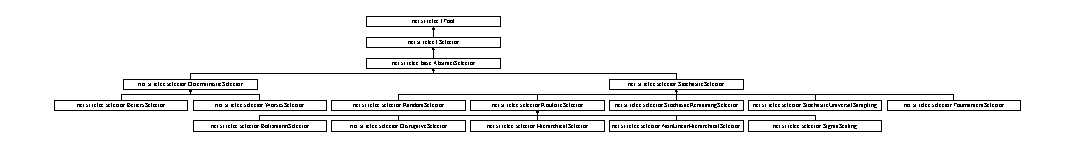
\includegraphics[height=1.543408cm]{classnet_1_1sf_1_1jclec_1_1base_1_1_abstract_selector}
\end{center}
\end{figure}
\subsection*{Public Member Functions}
\begin{DoxyCompactItemize}
\item 
\hyperlink{classnet_1_1sf_1_1jclec_1_1base_1_1_abstract_selector_af6ff5b38a9659ca10544079baa7acd90}{Abstract\-Selector} ()
\item 
\hyperlink{classnet_1_1sf_1_1jclec_1_1base_1_1_abstract_selector_a775ba98ec610490a02e1dedf7d04bace}{Abstract\-Selector} (\hyperlink{interfacenet_1_1sf_1_1jclec_1_1_i_system}{I\-System} \hyperlink{classnet_1_1sf_1_1jclec_1_1base_1_1_abstract_selector_a4304fe5c27aa7631dc91678d22473b94}{context})
\item 
void \hyperlink{classnet_1_1sf_1_1jclec_1_1base_1_1_abstract_selector_a58922faccb1ed92b428192814f72f573}{contextualize} (\hyperlink{interfacenet_1_1sf_1_1jclec_1_1_i_system}{I\-System} \hyperlink{classnet_1_1sf_1_1jclec_1_1base_1_1_abstract_selector_a4304fe5c27aa7631dc91678d22473b94}{context})
\item 
List$<$ \hyperlink{interfacenet_1_1sf_1_1jclec_1_1_i_individual}{I\-Individual} $>$ \hyperlink{classnet_1_1sf_1_1jclec_1_1base_1_1_abstract_selector_a1458859cb6d679871bee23ea7fc498cd}{select} (List$<$ \hyperlink{interfacenet_1_1sf_1_1jclec_1_1_i_individual}{I\-Individual} $>$ src)
\item 
List$<$ \hyperlink{interfacenet_1_1sf_1_1jclec_1_1_i_individual}{I\-Individual} $>$ \hyperlink{classnet_1_1sf_1_1jclec_1_1base_1_1_abstract_selector_a331626c701ad91e9fb39688485e69828}{select} (List$<$ \hyperlink{interfacenet_1_1sf_1_1jclec_1_1_i_individual}{I\-Individual} $>$ src, int nofsel)
\item 
List$<$ \hyperlink{interfacenet_1_1sf_1_1jclec_1_1_i_individual}{I\-Individual} $>$ \hyperlink{classnet_1_1sf_1_1jclec_1_1base_1_1_abstract_selector_abc984de4221a638e48ead2e0c0bc3a08}{select} (List$<$ \hyperlink{interfacenet_1_1sf_1_1jclec_1_1_i_individual}{I\-Individual} $>$ src, int nofsel, boolean repeat)
\end{DoxyCompactItemize}
\subsection*{Protected Member Functions}
\begin{DoxyCompactItemize}
\item 
abstract void \hyperlink{classnet_1_1sf_1_1jclec_1_1base_1_1_abstract_selector_a0c5d9cb96fef9786e272b9edd811111e}{prepare\-Selection} ()
\item 
abstract \hyperlink{interfacenet_1_1sf_1_1jclec_1_1_i_individual}{I\-Individual} \hyperlink{classnet_1_1sf_1_1jclec_1_1base_1_1_abstract_selector_aa2ccb539c608db9c14ebbc763807b95a}{select\-Next} ()
\end{DoxyCompactItemize}
\subsection*{Protected Attributes}
\begin{DoxyCompactItemize}
\item 
\hyperlink{interfacenet_1_1sf_1_1jclec_1_1_i_population}{I\-Population} \hyperlink{classnet_1_1sf_1_1jclec_1_1base_1_1_abstract_selector_a4304fe5c27aa7631dc91678d22473b94}{context}
\item 
transient List$<$ \hyperlink{interfacenet_1_1sf_1_1jclec_1_1_i_individual}{I\-Individual} $>$ \hyperlink{classnet_1_1sf_1_1jclec_1_1base_1_1_abstract_selector_abb353bff6e96b278329dff246d5648e4}{actsrc}
\item 
transient int \hyperlink{classnet_1_1sf_1_1jclec_1_1base_1_1_abstract_selector_ad405a34fb8182ec982b759fb0f6f8b2b}{actsrcsz}
\end{DoxyCompactItemize}


\subsection{Detailed Description}
\hyperlink{interfacenet_1_1sf_1_1jclec_1_1_i_selector}{I\-Selector} abstract implementation.

\begin{DoxyAuthor}{Author}
Sebastian Ventura 
\end{DoxyAuthor}


\subsection{Constructor \& Destructor Documentation}
\hypertarget{classnet_1_1sf_1_1jclec_1_1base_1_1_abstract_selector_af6ff5b38a9659ca10544079baa7acd90}{\index{net\-::sf\-::jclec\-::base\-::\-Abstract\-Selector@{net\-::sf\-::jclec\-::base\-::\-Abstract\-Selector}!Abstract\-Selector@{Abstract\-Selector}}
\index{Abstract\-Selector@{Abstract\-Selector}!net::sf::jclec::base::AbstractSelector@{net\-::sf\-::jclec\-::base\-::\-Abstract\-Selector}}
\subsubsection[{Abstract\-Selector}]{\setlength{\rightskip}{0pt plus 5cm}net.\-sf.\-jclec.\-base.\-Abstract\-Selector.\-Abstract\-Selector (
\begin{DoxyParamCaption}
{}
\end{DoxyParamCaption}
)}}\label{classnet_1_1sf_1_1jclec_1_1base_1_1_abstract_selector_af6ff5b38a9659ca10544079baa7acd90}
Empty selector. \hypertarget{classnet_1_1sf_1_1jclec_1_1base_1_1_abstract_selector_a775ba98ec610490a02e1dedf7d04bace}{\index{net\-::sf\-::jclec\-::base\-::\-Abstract\-Selector@{net\-::sf\-::jclec\-::base\-::\-Abstract\-Selector}!Abstract\-Selector@{Abstract\-Selector}}
\index{Abstract\-Selector@{Abstract\-Selector}!net::sf::jclec::base::AbstractSelector@{net\-::sf\-::jclec\-::base\-::\-Abstract\-Selector}}
\subsubsection[{Abstract\-Selector}]{\setlength{\rightskip}{0pt plus 5cm}net.\-sf.\-jclec.\-base.\-Abstract\-Selector.\-Abstract\-Selector (
\begin{DoxyParamCaption}
\item[{{\bf I\-System}}]{context}
\end{DoxyParamCaption}
)}}\label{classnet_1_1sf_1_1jclec_1_1base_1_1_abstract_selector_a775ba98ec610490a02e1dedf7d04bace}
Constructor that contextualizes selector. This method is used in algorithms internally. 

\subsection{Member Function Documentation}
\hypertarget{classnet_1_1sf_1_1jclec_1_1base_1_1_abstract_selector_a58922faccb1ed92b428192814f72f573}{\index{net\-::sf\-::jclec\-::base\-::\-Abstract\-Selector@{net\-::sf\-::jclec\-::base\-::\-Abstract\-Selector}!contextualize@{contextualize}}
\index{contextualize@{contextualize}!net::sf::jclec::base::AbstractSelector@{net\-::sf\-::jclec\-::base\-::\-Abstract\-Selector}}
\subsubsection[{contextualize}]{\setlength{\rightskip}{0pt plus 5cm}void net.\-sf.\-jclec.\-base.\-Abstract\-Selector.\-contextualize (
\begin{DoxyParamCaption}
\item[{{\bf I\-System}}]{context}
\end{DoxyParamCaption}
)}}\label{classnet_1_1sf_1_1jclec_1_1base_1_1_abstract_selector_a58922faccb1ed92b428192814f72f573}
Set the system where ...


\begin{DoxyParams}{Parameters}
{\em context} & Execution context\\
\hline
\end{DoxyParams}
 

Implements \hyperlink{interfacenet_1_1sf_1_1jclec_1_1_i_tool_aa11b3e046b7f38e40eb4f8c72a9a2102}{net.\-sf.\-jclec.\-I\-Tool}.

\hypertarget{classnet_1_1sf_1_1jclec_1_1base_1_1_abstract_selector_a0c5d9cb96fef9786e272b9edd811111e}{\index{net\-::sf\-::jclec\-::base\-::\-Abstract\-Selector@{net\-::sf\-::jclec\-::base\-::\-Abstract\-Selector}!prepare\-Selection@{prepare\-Selection}}
\index{prepare\-Selection@{prepare\-Selection}!net::sf::jclec::base::AbstractSelector@{net\-::sf\-::jclec\-::base\-::\-Abstract\-Selector}}
\subsubsection[{prepare\-Selection}]{\setlength{\rightskip}{0pt plus 5cm}abstract void net.\-sf.\-jclec.\-base.\-Abstract\-Selector.\-prepare\-Selection (
\begin{DoxyParamCaption}
{}
\end{DoxyParamCaption}
)\hspace{0.3cm}{\ttfamily [protected]}, {\ttfamily [pure virtual]}}}\label{classnet_1_1sf_1_1jclec_1_1base_1_1_abstract_selector_a0c5d9cb96fef9786e272b9edd811111e}
Prepare the selection process. 

Implemented in \hyperlink{classnet_1_1sf_1_1jclec_1_1selector_1_1_boltzmann_selector_a6edd0857b95771a97a1484b98ebc2fb0}{net.\-sf.\-jclec.\-selector.\-Boltzmann\-Selector}, \hyperlink{classnet_1_1sf_1_1jclec_1_1selector_1_1_tournament_selector_a9748d4136a0ceaaf1fac9689d56479e0}{net.\-sf.\-jclec.\-selector.\-Tournament\-Selector}, \hyperlink{classnet_1_1sf_1_1jclec_1_1selector_1_1_stochastic_universal_sampling_a96de01df1c80595d744f3c706699d927}{net.\-sf.\-jclec.\-selector.\-Stochastic\-Universal\-Sampling}, \hyperlink{classnet_1_1sf_1_1jclec_1_1selector_1_1_worses_selector_a826fea71513580a0fcbf2b9fca7782f6}{net.\-sf.\-jclec.\-selector.\-Worses\-Selector}, \hyperlink{classnet_1_1sf_1_1jclec_1_1selector_1_1_betters_selector_a6e1bf12a092b5d3cc1ac8010aa032480}{net.\-sf.\-jclec.\-selector.\-Betters\-Selector}, \hyperlink{classnet_1_1sf_1_1jclec_1_1selector_1_1_stochastic_remaining_selector_aafb59c95f8c8324bfe7ca47311879773}{net.\-sf.\-jclec.\-selector.\-Stochastic\-Remaining\-Selector}, \hyperlink{classnet_1_1sf_1_1jclec_1_1selector_1_1_hierarchical_selector_a9365e41d27d09e4839866388cd3bbe3a}{net.\-sf.\-jclec.\-selector.\-Hierarchical\-Selector}, \hyperlink{classnet_1_1sf_1_1jclec_1_1selector_1_1_disruptive_selector_a8f9d0833b098d9d1dc91e24804de5043}{net.\-sf.\-jclec.\-selector.\-Disruptive\-Selector}, \hyperlink{classnet_1_1sf_1_1jclec_1_1selector_1_1_sigma_scaling_ad513ba7df2641cb9116ddc3e277dc508}{net.\-sf.\-jclec.\-selector.\-Sigma\-Scaling}, \hyperlink{classnet_1_1sf_1_1jclec_1_1selector_1_1_non_linear_hierarchical_selector_a83a69260e6b0ccf084e15e4fe0ace62d}{net.\-sf.\-jclec.\-selector.\-Non\-Linear\-Hierarchical\-Selector}, \hyperlink{classnet_1_1sf_1_1jclec_1_1selector_1_1_random_selector_a560e1811c364ea7fabf92ced37f6e9ef}{net.\-sf.\-jclec.\-selector.\-Random\-Selector}, and \hyperlink{classnet_1_1sf_1_1jclec_1_1selector_1_1_roulette_selector_a1ce03c3e978aadacffd10309c36d82db}{net.\-sf.\-jclec.\-selector.\-Roulette\-Selector}.

\hypertarget{classnet_1_1sf_1_1jclec_1_1base_1_1_abstract_selector_a1458859cb6d679871bee23ea7fc498cd}{\index{net\-::sf\-::jclec\-::base\-::\-Abstract\-Selector@{net\-::sf\-::jclec\-::base\-::\-Abstract\-Selector}!select@{select}}
\index{select@{select}!net::sf::jclec::base::AbstractSelector@{net\-::sf\-::jclec\-::base\-::\-Abstract\-Selector}}
\subsubsection[{select}]{\setlength{\rightskip}{0pt plus 5cm}List$<${\bf I\-Individual}$>$ net.\-sf.\-jclec.\-base.\-Abstract\-Selector.\-select (
\begin{DoxyParamCaption}
\item[{List$<$ {\bf I\-Individual} $>$}]{src}
\end{DoxyParamCaption}
)}}\label{classnet_1_1sf_1_1jclec_1_1base_1_1_abstract_selector_a1458859cb6d679871bee23ea7fc498cd}
Selection method.


\begin{DoxyParams}{Parameters}
{\em source} & Source set\\
\hline
\end{DoxyParams}
\begin{DoxyReturn}{Returns}
Selected individuals
\end{DoxyReturn}
 

Implements \hyperlink{interfacenet_1_1sf_1_1jclec_1_1_i_selector_a271fa45c6619e39126b64d0d7db83d17}{net.\-sf.\-jclec.\-I\-Selector}.

\hypertarget{classnet_1_1sf_1_1jclec_1_1base_1_1_abstract_selector_a331626c701ad91e9fb39688485e69828}{\index{net\-::sf\-::jclec\-::base\-::\-Abstract\-Selector@{net\-::sf\-::jclec\-::base\-::\-Abstract\-Selector}!select@{select}}
\index{select@{select}!net::sf::jclec::base::AbstractSelector@{net\-::sf\-::jclec\-::base\-::\-Abstract\-Selector}}
\subsubsection[{select}]{\setlength{\rightskip}{0pt plus 5cm}List$<${\bf I\-Individual}$>$ net.\-sf.\-jclec.\-base.\-Abstract\-Selector.\-select (
\begin{DoxyParamCaption}
\item[{List$<$ {\bf I\-Individual} $>$}]{src, }
\item[{int}]{nofsel}
\end{DoxyParamCaption}
)}}\label{classnet_1_1sf_1_1jclec_1_1base_1_1_abstract_selector_a331626c701ad91e9fb39688485e69828}
Alternative selection method.


\begin{DoxyParams}{Parameters}
{\em source} & Source set \\
\hline
{\em nofsel} & Number of individuals to select\\
\hline
\end{DoxyParams}
\begin{DoxyReturn}{Returns}
Selected individuals
\end{DoxyReturn}
 

Implements \hyperlink{interfacenet_1_1sf_1_1jclec_1_1_i_selector_a40ef927639aa3cf51b1ffe4bb43e0fde}{net.\-sf.\-jclec.\-I\-Selector}.

\hypertarget{classnet_1_1sf_1_1jclec_1_1base_1_1_abstract_selector_abc984de4221a638e48ead2e0c0bc3a08}{\index{net\-::sf\-::jclec\-::base\-::\-Abstract\-Selector@{net\-::sf\-::jclec\-::base\-::\-Abstract\-Selector}!select@{select}}
\index{select@{select}!net::sf::jclec::base::AbstractSelector@{net\-::sf\-::jclec\-::base\-::\-Abstract\-Selector}}
\subsubsection[{select}]{\setlength{\rightskip}{0pt plus 5cm}List$<${\bf I\-Individual}$>$ net.\-sf.\-jclec.\-base.\-Abstract\-Selector.\-select (
\begin{DoxyParamCaption}
\item[{List$<$ {\bf I\-Individual} $>$}]{source, }
\item[{int}]{nofsel, }
\item[{boolean}]{repeat}
\end{DoxyParamCaption}
)}}\label{classnet_1_1sf_1_1jclec_1_1base_1_1_abstract_selector_abc984de4221a638e48ead2e0c0bc3a08}
Alternative selection method.


\begin{DoxyParams}{Parameters}
{\em source} & Source set \\
\hline
{\em nofsel} & Number of individuals to select \\
\hline
{\em repeat} & Is selection of repeated individuals allowed?\\
\hline
\end{DoxyParams}
\begin{DoxyReturn}{Returns}
Selected individuals 
\end{DoxyReturn}


Implements \hyperlink{interfacenet_1_1sf_1_1jclec_1_1_i_selector_ac2447d10f2f8164df4f4c94c12db3751}{net.\-sf.\-jclec.\-I\-Selector}.

\hypertarget{classnet_1_1sf_1_1jclec_1_1base_1_1_abstract_selector_aa2ccb539c608db9c14ebbc763807b95a}{\index{net\-::sf\-::jclec\-::base\-::\-Abstract\-Selector@{net\-::sf\-::jclec\-::base\-::\-Abstract\-Selector}!select\-Next@{select\-Next}}
\index{select\-Next@{select\-Next}!net::sf::jclec::base::AbstractSelector@{net\-::sf\-::jclec\-::base\-::\-Abstract\-Selector}}
\subsubsection[{select\-Next}]{\setlength{\rightskip}{0pt plus 5cm}abstract {\bf I\-Individual} net.\-sf.\-jclec.\-base.\-Abstract\-Selector.\-select\-Next (
\begin{DoxyParamCaption}
{}
\end{DoxyParamCaption}
)\hspace{0.3cm}{\ttfamily [protected]}, {\ttfamily [pure virtual]}}}\label{classnet_1_1sf_1_1jclec_1_1base_1_1_abstract_selector_aa2ccb539c608db9c14ebbc763807b95a}
Selects an individual (in the context of a selection process).

\begin{DoxyReturn}{Returns}
Selected individual 
\end{DoxyReturn}


Implemented in \hyperlink{classnet_1_1sf_1_1jclec_1_1selector_1_1_stochastic_universal_sampling_a98f656114c234fdc5ddcf8e532bebe22}{net.\-sf.\-jclec.\-selector.\-Stochastic\-Universal\-Sampling}, \hyperlink{classnet_1_1sf_1_1jclec_1_1selector_1_1_tournament_selector_af2743032d654d6bac87391ddfab4cd1a}{net.\-sf.\-jclec.\-selector.\-Tournament\-Selector}, \hyperlink{classnet_1_1sf_1_1jclec_1_1selector_1_1_stochastic_remaining_selector_aa334f3ed9889328cc51632ccf178123b}{net.\-sf.\-jclec.\-selector.\-Stochastic\-Remaining\-Selector}, \hyperlink{classnet_1_1sf_1_1jclec_1_1selector_1_1_worses_selector_a11a1329db7f422cc0a3e3292a6ed46a1}{net.\-sf.\-jclec.\-selector.\-Worses\-Selector}, \hyperlink{classnet_1_1sf_1_1jclec_1_1selector_1_1_betters_selector_aafc05c782c8e38e6c39130fc3c1fa1a3}{net.\-sf.\-jclec.\-selector.\-Betters\-Selector}, \hyperlink{classnet_1_1sf_1_1jclec_1_1selector_1_1_roulette_selector_a4403c44d775ee37fd7c8d69662106499}{net.\-sf.\-jclec.\-selector.\-Roulette\-Selector}, and \hyperlink{classnet_1_1sf_1_1jclec_1_1selector_1_1_random_selector_a0771964cb15ffb2de63ec98292bddcdd}{net.\-sf.\-jclec.\-selector.\-Random\-Selector}.



\subsection{Member Data Documentation}
\hypertarget{classnet_1_1sf_1_1jclec_1_1base_1_1_abstract_selector_abb353bff6e96b278329dff246d5648e4}{\index{net\-::sf\-::jclec\-::base\-::\-Abstract\-Selector@{net\-::sf\-::jclec\-::base\-::\-Abstract\-Selector}!actsrc@{actsrc}}
\index{actsrc@{actsrc}!net::sf::jclec::base::AbstractSelector@{net\-::sf\-::jclec\-::base\-::\-Abstract\-Selector}}
\subsubsection[{actsrc}]{\setlength{\rightskip}{0pt plus 5cm}transient List$<${\bf I\-Individual}$>$ net.\-sf.\-jclec.\-base.\-Abstract\-Selector.\-actsrc\hspace{0.3cm}{\ttfamily [protected]}}}\label{classnet_1_1sf_1_1jclec_1_1base_1_1_abstract_selector_abb353bff6e96b278329dff246d5648e4}
Source set \hypertarget{classnet_1_1sf_1_1jclec_1_1base_1_1_abstract_selector_ad405a34fb8182ec982b759fb0f6f8b2b}{\index{net\-::sf\-::jclec\-::base\-::\-Abstract\-Selector@{net\-::sf\-::jclec\-::base\-::\-Abstract\-Selector}!actsrcsz@{actsrcsz}}
\index{actsrcsz@{actsrcsz}!net::sf::jclec::base::AbstractSelector@{net\-::sf\-::jclec\-::base\-::\-Abstract\-Selector}}
\subsubsection[{actsrcsz}]{\setlength{\rightskip}{0pt plus 5cm}transient int net.\-sf.\-jclec.\-base.\-Abstract\-Selector.\-actsrcsz\hspace{0.3cm}{\ttfamily [protected]}}}\label{classnet_1_1sf_1_1jclec_1_1base_1_1_abstract_selector_ad405a34fb8182ec982b759fb0f6f8b2b}
Source set size \hypertarget{classnet_1_1sf_1_1jclec_1_1base_1_1_abstract_selector_a4304fe5c27aa7631dc91678d22473b94}{\index{net\-::sf\-::jclec\-::base\-::\-Abstract\-Selector@{net\-::sf\-::jclec\-::base\-::\-Abstract\-Selector}!context@{context}}
\index{context@{context}!net::sf::jclec::base::AbstractSelector@{net\-::sf\-::jclec\-::base\-::\-Abstract\-Selector}}
\subsubsection[{context}]{\setlength{\rightskip}{0pt plus 5cm}{\bf I\-Population} net.\-sf.\-jclec.\-base.\-Abstract\-Selector.\-context\hspace{0.3cm}{\ttfamily [protected]}}}\label{classnet_1_1sf_1_1jclec_1_1base_1_1_abstract_selector_a4304fe5c27aa7631dc91678d22473b94}
Execution context 

The documentation for this class was generated from the following file\-:\begin{DoxyCompactItemize}
\item 
src/main/java/net/sf/jclec/base/Abstract\-Selector.\-java\end{DoxyCompactItemize}

\hypertarget{classnet_1_1sf_1_1jclec_1_1realarray_1_1rec_1_1_algebraic_connectives}{\section{net.\-sf.\-jclec.\-realarray.\-rec.\-Algebraic\-Connectives Class Reference}
\label{classnet_1_1sf_1_1jclec_1_1realarray_1_1rec_1_1_algebraic_connectives}\index{net.\-sf.\-jclec.\-realarray.\-rec.\-Algebraic\-Connectives@{net.\-sf.\-jclec.\-realarray.\-rec.\-Algebraic\-Connectives}}
}
Inheritance diagram for net.\-sf.\-jclec.\-realarray.\-rec.\-Algebraic\-Connectives\-:\begin{figure}[H]
\begin{center}
\leavevmode
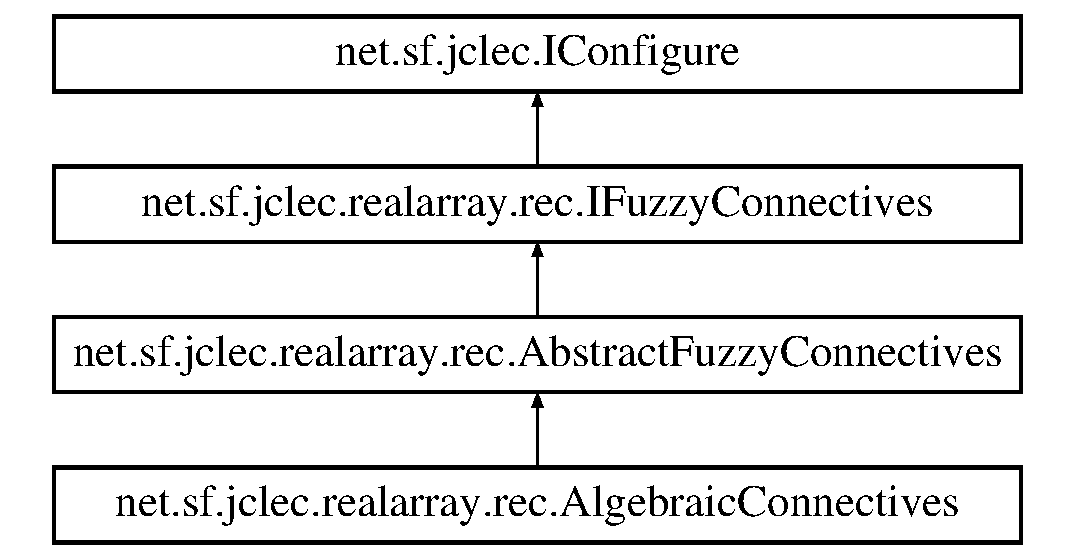
\includegraphics[height=4.000000cm]{classnet_1_1sf_1_1jclec_1_1realarray_1_1rec_1_1_algebraic_connectives}
\end{center}
\end{figure}
\subsection*{Public Member Functions}
\begin{DoxyCompactItemize}
\item 
\hyperlink{classnet_1_1sf_1_1jclec_1_1realarray_1_1rec_1_1_algebraic_connectives_a26350ab501c2c71341af01ed4f3fe77f}{Algebraic\-Connectives} ()
\item 
double \hyperlink{classnet_1_1sf_1_1jclec_1_1realarray_1_1rec_1_1_algebraic_connectives_a218066c3869342ae5099c6791cff33a6}{m} (double x, double y)
\item 
double \hyperlink{classnet_1_1sf_1_1jclec_1_1realarray_1_1rec_1_1_algebraic_connectives_ad95901413e7d84a800693a10ef3f7ac6}{s} (double x, double y)
\item 
double \hyperlink{classnet_1_1sf_1_1jclec_1_1realarray_1_1rec_1_1_algebraic_connectives_a4d773e09a9edc3d2311b8c466fa2433f}{f} (double x, double y)
\item 
double \hyperlink{classnet_1_1sf_1_1jclec_1_1realarray_1_1rec_1_1_algebraic_connectives_a3055caa9ec556a01abbd07d56353addc}{l} (double x, double y)
\end{DoxyCompactItemize}


\subsection{Detailed Description}
Algebraic Connectives

\begin{DoxyAuthor}{Author}
Alberto Lamarca-\/\-Rosales 

Sebastian Ventura 
\end{DoxyAuthor}


\subsection{Constructor \& Destructor Documentation}
\hypertarget{classnet_1_1sf_1_1jclec_1_1realarray_1_1rec_1_1_algebraic_connectives_a26350ab501c2c71341af01ed4f3fe77f}{\index{net\-::sf\-::jclec\-::realarray\-::rec\-::\-Algebraic\-Connectives@{net\-::sf\-::jclec\-::realarray\-::rec\-::\-Algebraic\-Connectives}!Algebraic\-Connectives@{Algebraic\-Connectives}}
\index{Algebraic\-Connectives@{Algebraic\-Connectives}!net::sf::jclec::realarray::rec::AlgebraicConnectives@{net\-::sf\-::jclec\-::realarray\-::rec\-::\-Algebraic\-Connectives}}
\subsubsection[{Algebraic\-Connectives}]{\setlength{\rightskip}{0pt plus 5cm}net.\-sf.\-jclec.\-realarray.\-rec.\-Algebraic\-Connectives.\-Algebraic\-Connectives (
\begin{DoxyParamCaption}
{}
\end{DoxyParamCaption}
)}}\label{classnet_1_1sf_1_1jclec_1_1realarray_1_1rec_1_1_algebraic_connectives_a26350ab501c2c71341af01ed4f3fe77f}
Empty constructor 

\subsection{Member Function Documentation}
\hypertarget{classnet_1_1sf_1_1jclec_1_1realarray_1_1rec_1_1_algebraic_connectives_a4d773e09a9edc3d2311b8c466fa2433f}{\index{net\-::sf\-::jclec\-::realarray\-::rec\-::\-Algebraic\-Connectives@{net\-::sf\-::jclec\-::realarray\-::rec\-::\-Algebraic\-Connectives}!f@{f}}
\index{f@{f}!net::sf::jclec::realarray::rec::AlgebraicConnectives@{net\-::sf\-::jclec\-::realarray\-::rec\-::\-Algebraic\-Connectives}}
\subsubsection[{f}]{\setlength{\rightskip}{0pt plus 5cm}double net.\-sf.\-jclec.\-realarray.\-rec.\-Algebraic\-Connectives.\-f (
\begin{DoxyParamCaption}
\item[{double}]{x, }
\item[{double}]{y}
\end{DoxyParamCaption}
)\hspace{0.3cm}{\ttfamily [virtual]}}}\label{classnet_1_1sf_1_1jclec_1_1realarray_1_1rec_1_1_algebraic_connectives_a4d773e09a9edc3d2311b8c466fa2433f}
Algebraic Function f 

Implements \hyperlink{interfacenet_1_1sf_1_1jclec_1_1realarray_1_1rec_1_1_i_fuzzy_connectives_a970200edf4d66083e0ad040096783c35}{net.\-sf.\-jclec.\-realarray.\-rec.\-I\-Fuzzy\-Connectives}.

\hypertarget{classnet_1_1sf_1_1jclec_1_1realarray_1_1rec_1_1_algebraic_connectives_a3055caa9ec556a01abbd07d56353addc}{\index{net\-::sf\-::jclec\-::realarray\-::rec\-::\-Algebraic\-Connectives@{net\-::sf\-::jclec\-::realarray\-::rec\-::\-Algebraic\-Connectives}!l@{l}}
\index{l@{l}!net::sf::jclec::realarray::rec::AlgebraicConnectives@{net\-::sf\-::jclec\-::realarray\-::rec\-::\-Algebraic\-Connectives}}
\subsubsection[{l}]{\setlength{\rightskip}{0pt plus 5cm}double net.\-sf.\-jclec.\-realarray.\-rec.\-Algebraic\-Connectives.\-l (
\begin{DoxyParamCaption}
\item[{double}]{x, }
\item[{double}]{y}
\end{DoxyParamCaption}
)\hspace{0.3cm}{\ttfamily [virtual]}}}\label{classnet_1_1sf_1_1jclec_1_1realarray_1_1rec_1_1_algebraic_connectives_a3055caa9ec556a01abbd07d56353addc}
Algebraic Function l 

Implements \hyperlink{interfacenet_1_1sf_1_1jclec_1_1realarray_1_1rec_1_1_i_fuzzy_connectives_a0cea5560723101682211330bba9e20e4}{net.\-sf.\-jclec.\-realarray.\-rec.\-I\-Fuzzy\-Connectives}.

\hypertarget{classnet_1_1sf_1_1jclec_1_1realarray_1_1rec_1_1_algebraic_connectives_a218066c3869342ae5099c6791cff33a6}{\index{net\-::sf\-::jclec\-::realarray\-::rec\-::\-Algebraic\-Connectives@{net\-::sf\-::jclec\-::realarray\-::rec\-::\-Algebraic\-Connectives}!m@{m}}
\index{m@{m}!net::sf::jclec::realarray::rec::AlgebraicConnectives@{net\-::sf\-::jclec\-::realarray\-::rec\-::\-Algebraic\-Connectives}}
\subsubsection[{m}]{\setlength{\rightskip}{0pt plus 5cm}double net.\-sf.\-jclec.\-realarray.\-rec.\-Algebraic\-Connectives.\-m (
\begin{DoxyParamCaption}
\item[{double}]{x, }
\item[{double}]{y}
\end{DoxyParamCaption}
)\hspace{0.3cm}{\ttfamily [virtual]}}}\label{classnet_1_1sf_1_1jclec_1_1realarray_1_1rec_1_1_algebraic_connectives_a218066c3869342ae5099c6791cff33a6}
Algebraic Function m 

Implements \hyperlink{interfacenet_1_1sf_1_1jclec_1_1realarray_1_1rec_1_1_i_fuzzy_connectives_acd07fed683410b0147e04075b8d6aea6}{net.\-sf.\-jclec.\-realarray.\-rec.\-I\-Fuzzy\-Connectives}.

\hypertarget{classnet_1_1sf_1_1jclec_1_1realarray_1_1rec_1_1_algebraic_connectives_ad95901413e7d84a800693a10ef3f7ac6}{\index{net\-::sf\-::jclec\-::realarray\-::rec\-::\-Algebraic\-Connectives@{net\-::sf\-::jclec\-::realarray\-::rec\-::\-Algebraic\-Connectives}!s@{s}}
\index{s@{s}!net::sf::jclec::realarray::rec::AlgebraicConnectives@{net\-::sf\-::jclec\-::realarray\-::rec\-::\-Algebraic\-Connectives}}
\subsubsection[{s}]{\setlength{\rightskip}{0pt plus 5cm}double net.\-sf.\-jclec.\-realarray.\-rec.\-Algebraic\-Connectives.\-s (
\begin{DoxyParamCaption}
\item[{double}]{x, }
\item[{double}]{y}
\end{DoxyParamCaption}
)\hspace{0.3cm}{\ttfamily [virtual]}}}\label{classnet_1_1sf_1_1jclec_1_1realarray_1_1rec_1_1_algebraic_connectives_ad95901413e7d84a800693a10ef3f7ac6}
Algebraic Function s 

Implements \hyperlink{interfacenet_1_1sf_1_1jclec_1_1realarray_1_1rec_1_1_i_fuzzy_connectives_a2ae764e485434e088a8128a9e2bea734}{net.\-sf.\-jclec.\-realarray.\-rec.\-I\-Fuzzy\-Connectives}.



The documentation for this class was generated from the following file\-:\begin{DoxyCompactItemize}
\item 
src/main/java/net/sf/jclec/realarray/rec/Algebraic\-Connectives.\-java\end{DoxyCompactItemize}

\hypertarget{classnet_1_1sf_1_1jclec_1_1_algorithm_event}{\section{net.\-sf.\-jclec.\-Algorithm\-Event Class Reference}
\label{classnet_1_1sf_1_1jclec_1_1_algorithm_event}\index{net.\-sf.\-jclec.\-Algorithm\-Event@{net.\-sf.\-jclec.\-Algorithm\-Event}}
}


Inherits Event\-Object.

\subsection*{Public Member Functions}
\begin{DoxyCompactItemize}
\item 
\hyperlink{classnet_1_1sf_1_1jclec_1_1_algorithm_event_a059a3f11bca8765181ccbff53f452047}{Algorithm\-Event} (I\-Algorithm \hyperlink{classnet_1_1sf_1_1jclec_1_1_algorithm_event_ae3332a37fbfc99e4c5eea8b0748c1e77}{algorithm})
\item 
\hyperlink{classnet_1_1sf_1_1jclec_1_1_algorithm_event_ab18000f022656286ec8746b2ee936cf7}{Algorithm\-Event} (I\-Algorithm \hyperlink{classnet_1_1sf_1_1jclec_1_1_algorithm_event_ae3332a37fbfc99e4c5eea8b0748c1e77}{algorithm}, Exception \hyperlink{classnet_1_1sf_1_1jclec_1_1_algorithm_event_aa8ed9d4190a583cbe4873dac89fdef7c}{exception})
\item 
final I\-Algorithm \hyperlink{classnet_1_1sf_1_1jclec_1_1_algorithm_event_a3cfac8934c76ad650ceda4280a44f66f}{get\-Algorithm} ()
\item 
final Exception \hyperlink{classnet_1_1sf_1_1jclec_1_1_algorithm_event_a834fbc754fae9b30ab38ddffbed7f136}{get\-Exception} ()
\end{DoxyCompactItemize}
\subsection*{Protected Attributes}
\begin{DoxyCompactItemize}
\item 
I\-Algorithm \hyperlink{classnet_1_1sf_1_1jclec_1_1_algorithm_event_ae3332a37fbfc99e4c5eea8b0748c1e77}{algorithm}
\item 
Exception \hyperlink{classnet_1_1sf_1_1jclec_1_1_algorithm_event_aa8ed9d4190a583cbe4873dac89fdef7c}{exception}
\end{DoxyCompactItemize}


\subsection{Detailed Description}
Algorithm event.

\begin{DoxyAuthor}{Author}
Sebastian Ventura 
\end{DoxyAuthor}


\subsection{Constructor \& Destructor Documentation}
\hypertarget{classnet_1_1sf_1_1jclec_1_1_algorithm_event_a059a3f11bca8765181ccbff53f452047}{\index{net\-::sf\-::jclec\-::\-Algorithm\-Event@{net\-::sf\-::jclec\-::\-Algorithm\-Event}!Algorithm\-Event@{Algorithm\-Event}}
\index{Algorithm\-Event@{Algorithm\-Event}!net::sf::jclec::AlgorithmEvent@{net\-::sf\-::jclec\-::\-Algorithm\-Event}}
\subsubsection[{Algorithm\-Event}]{\setlength{\rightskip}{0pt plus 5cm}net.\-sf.\-jclec.\-Algorithm\-Event.\-Algorithm\-Event (
\begin{DoxyParamCaption}
\item[{I\-Algorithm}]{algorithm}
\end{DoxyParamCaption}
)}}\label{classnet_1_1sf_1_1jclec_1_1_algorithm_event_a059a3f11bca8765181ccbff53f452047}

\begin{DoxyParams}{Parameters}
{\em algorithm} & \\
\hline
\end{DoxyParams}
\hypertarget{classnet_1_1sf_1_1jclec_1_1_algorithm_event_ab18000f022656286ec8746b2ee936cf7}{\index{net\-::sf\-::jclec\-::\-Algorithm\-Event@{net\-::sf\-::jclec\-::\-Algorithm\-Event}!Algorithm\-Event@{Algorithm\-Event}}
\index{Algorithm\-Event@{Algorithm\-Event}!net::sf::jclec::AlgorithmEvent@{net\-::sf\-::jclec\-::\-Algorithm\-Event}}
\subsubsection[{Algorithm\-Event}]{\setlength{\rightskip}{0pt plus 5cm}net.\-sf.\-jclec.\-Algorithm\-Event.\-Algorithm\-Event (
\begin{DoxyParamCaption}
\item[{I\-Algorithm}]{algorithm, }
\item[{Exception}]{exception}
\end{DoxyParamCaption}
)}}\label{classnet_1_1sf_1_1jclec_1_1_algorithm_event_ab18000f022656286ec8746b2ee936cf7}

\begin{DoxyParams}{Parameters}
{\em algorithm} & \\
\hline
{\em exception} & \\
\hline
\end{DoxyParams}


\subsection{Member Function Documentation}
\hypertarget{classnet_1_1sf_1_1jclec_1_1_algorithm_event_a3cfac8934c76ad650ceda4280a44f66f}{\index{net\-::sf\-::jclec\-::\-Algorithm\-Event@{net\-::sf\-::jclec\-::\-Algorithm\-Event}!get\-Algorithm@{get\-Algorithm}}
\index{get\-Algorithm@{get\-Algorithm}!net::sf::jclec::AlgorithmEvent@{net\-::sf\-::jclec\-::\-Algorithm\-Event}}
\subsubsection[{get\-Algorithm}]{\setlength{\rightskip}{0pt plus 5cm}final I\-Algorithm net.\-sf.\-jclec.\-Algorithm\-Event.\-get\-Algorithm (
\begin{DoxyParamCaption}
{}
\end{DoxyParamCaption}
)}}\label{classnet_1_1sf_1_1jclec_1_1_algorithm_event_a3cfac8934c76ad650ceda4280a44f66f}
Access to algorithm.

\begin{DoxyReturn}{Returns}
Actual algorithm 
\end{DoxyReturn}
\hypertarget{classnet_1_1sf_1_1jclec_1_1_algorithm_event_a834fbc754fae9b30ab38ddffbed7f136}{\index{net\-::sf\-::jclec\-::\-Algorithm\-Event@{net\-::sf\-::jclec\-::\-Algorithm\-Event}!get\-Exception@{get\-Exception}}
\index{get\-Exception@{get\-Exception}!net::sf::jclec::AlgorithmEvent@{net\-::sf\-::jclec\-::\-Algorithm\-Event}}
\subsubsection[{get\-Exception}]{\setlength{\rightskip}{0pt plus 5cm}final Exception net.\-sf.\-jclec.\-Algorithm\-Event.\-get\-Exception (
\begin{DoxyParamCaption}
{}
\end{DoxyParamCaption}
)}}\label{classnet_1_1sf_1_1jclec_1_1_algorithm_event_a834fbc754fae9b30ab38ddffbed7f136}
Access to event exception.

\begin{DoxyReturn}{Returns}
Actual exception (null if none) 
\end{DoxyReturn}


\subsection{Member Data Documentation}
\hypertarget{classnet_1_1sf_1_1jclec_1_1_algorithm_event_ae3332a37fbfc99e4c5eea8b0748c1e77}{\index{net\-::sf\-::jclec\-::\-Algorithm\-Event@{net\-::sf\-::jclec\-::\-Algorithm\-Event}!algorithm@{algorithm}}
\index{algorithm@{algorithm}!net::sf::jclec::AlgorithmEvent@{net\-::sf\-::jclec\-::\-Algorithm\-Event}}
\subsubsection[{algorithm}]{\setlength{\rightskip}{0pt plus 5cm}I\-Algorithm net.\-sf.\-jclec.\-Algorithm\-Event.\-algorithm\hspace{0.3cm}{\ttfamily [protected]}}}\label{classnet_1_1sf_1_1jclec_1_1_algorithm_event_ae3332a37fbfc99e4c5eea8b0748c1e77}
Algorithm \hypertarget{classnet_1_1sf_1_1jclec_1_1_algorithm_event_aa8ed9d4190a583cbe4873dac89fdef7c}{\index{net\-::sf\-::jclec\-::\-Algorithm\-Event@{net\-::sf\-::jclec\-::\-Algorithm\-Event}!exception@{exception}}
\index{exception@{exception}!net::sf::jclec::AlgorithmEvent@{net\-::sf\-::jclec\-::\-Algorithm\-Event}}
\subsubsection[{exception}]{\setlength{\rightskip}{0pt plus 5cm}Exception net.\-sf.\-jclec.\-Algorithm\-Event.\-exception\hspace{0.3cm}{\ttfamily [protected]}}}\label{classnet_1_1sf_1_1jclec_1_1_algorithm_event_aa8ed9d4190a583cbe4873dac89fdef7c}
Exception 

The documentation for this class was generated from the following file\-:\begin{DoxyCompactItemize}
\item 
src/main/java/net/sf/jclec/Algorithm\-Event.\-java\end{DoxyCompactItemize}

\hypertarget{classnet_1_1sf_1_1jclec_1_1exprtree_1_1_all_expr_tree_tests}{\section{net.\-sf.\-jclec.\-exprtree.\-All\-Expr\-Tree\-Tests Class Reference}
\label{classnet_1_1sf_1_1jclec_1_1exprtree_1_1_all_expr_tree_tests}\index{net.\-sf.\-jclec.\-exprtree.\-All\-Expr\-Tree\-Tests@{net.\-sf.\-jclec.\-exprtree.\-All\-Expr\-Tree\-Tests}}
}


\subsection{Detailed Description}
All unit tests for exprtree, expretree.\-mut and exprtree.\-rec packages

\begin{DoxyAuthor}{Author}
Sebastian Ventura 
\end{DoxyAuthor}


The documentation for this class was generated from the following file\-:\begin{DoxyCompactItemize}
\item 
src/test/java/net/sf/jclec/exprtree/All\-Expr\-Tree\-Tests.\-java\end{DoxyCompactItemize}

\hypertarget{classnet_1_1sf_1_1jclec_1_1exprtree_1_1mut_1_1_all_nodes_mutator}{\section{net.\-sf.\-jclec.\-exprtree.\-mut.\-All\-Nodes\-Mutator Class Reference}
\label{classnet_1_1sf_1_1jclec_1_1exprtree_1_1mut_1_1_all_nodes_mutator}\index{net.\-sf.\-jclec.\-exprtree.\-mut.\-All\-Nodes\-Mutator@{net.\-sf.\-jclec.\-exprtree.\-mut.\-All\-Nodes\-Mutator}}
}
Inheritance diagram for net.\-sf.\-jclec.\-exprtree.\-mut.\-All\-Nodes\-Mutator\-:\begin{figure}[H]
\begin{center}
\leavevmode
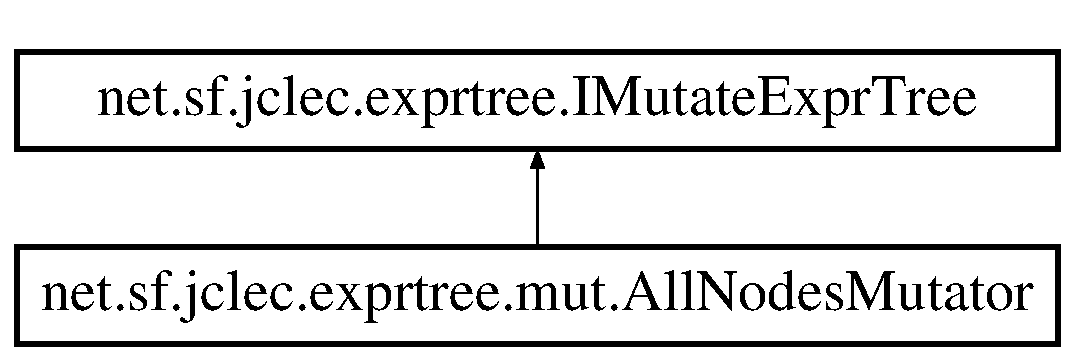
\includegraphics[height=2.000000cm]{classnet_1_1sf_1_1jclec_1_1exprtree_1_1mut_1_1_all_nodes_mutator}
\end{center}
\end{figure}
\subsection*{Public Member Functions}
\begin{DoxyCompactItemize}
\item 
\hyperlink{classnet_1_1sf_1_1jclec_1_1exprtree_1_1_expr_tree}{Expr\-Tree} \hyperlink{classnet_1_1sf_1_1jclec_1_1exprtree_1_1mut_1_1_all_nodes_mutator_a7e052b0f77eb63ad293f359dee697fc6}{mutate\-Expr\-Tree} (\hyperlink{classnet_1_1sf_1_1jclec_1_1exprtree_1_1_expr_tree}{Expr\-Tree} ptree, \hyperlink{classnet_1_1sf_1_1jclec_1_1exprtree_1_1_expr_tree_schema}{Expr\-Tree\-Schema} schema, \hyperlink{interfacenet_1_1sf_1_1jclec_1_1util_1_1random_1_1_i_rand_gen}{I\-Rand\-Gen} randgen)
\end{DoxyCompactItemize}


\subsection{Detailed Description}
Took each and every node in the computer program and replaced it with another randomly chosen block of the same return type and arity.

\begin{DoxyAuthor}{Author}
Sebastian Ventura 
\end{DoxyAuthor}


\subsection{Member Function Documentation}
\hypertarget{classnet_1_1sf_1_1jclec_1_1exprtree_1_1mut_1_1_all_nodes_mutator_a7e052b0f77eb63ad293f359dee697fc6}{\index{net\-::sf\-::jclec\-::exprtree\-::mut\-::\-All\-Nodes\-Mutator@{net\-::sf\-::jclec\-::exprtree\-::mut\-::\-All\-Nodes\-Mutator}!mutate\-Expr\-Tree@{mutate\-Expr\-Tree}}
\index{mutate\-Expr\-Tree@{mutate\-Expr\-Tree}!net::sf::jclec::exprtree::mut::AllNodesMutator@{net\-::sf\-::jclec\-::exprtree\-::mut\-::\-All\-Nodes\-Mutator}}
\subsubsection[{mutate\-Expr\-Tree}]{\setlength{\rightskip}{0pt plus 5cm}{\bf Expr\-Tree} net.\-sf.\-jclec.\-exprtree.\-mut.\-All\-Nodes\-Mutator.\-mutate\-Expr\-Tree (
\begin{DoxyParamCaption}
\item[{{\bf Expr\-Tree}}]{tree, }
\item[{{\bf Expr\-Tree\-Schema}}]{tree\-Schema, }
\item[{{\bf I\-Rand\-Gen}}]{randgen}
\end{DoxyParamCaption}
)\hspace{0.3cm}{\ttfamily [virtual]}}}\label{classnet_1_1sf_1_1jclec_1_1exprtree_1_1mut_1_1_all_nodes_mutator_a7e052b0f77eb63ad293f359dee697fc6}

\begin{DoxyParams}{Parameters}
{\em tree} & \\
\hline
{\em tree\-Schema} & \\
\hline
{\em randgen} & \\
\hline
\end{DoxyParams}
\begin{DoxyReturn}{Returns}
A new expression tree 
\end{DoxyReturn}


Implements \hyperlink{interfacenet_1_1sf_1_1jclec_1_1exprtree_1_1_i_mutate_expr_tree_aa3d6090a4580d9cd5f0e6a834df8a535}{net.\-sf.\-jclec.\-exprtree.\-I\-Mutate\-Expr\-Tree}.



The documentation for this class was generated from the following file\-:\begin{DoxyCompactItemize}
\item 
src/main/java/net/sf/jclec/exprtree/mut/All\-Nodes\-Mutator.\-java\end{DoxyCompactItemize}

\hypertarget{classnet_1_1sf_1_1jclec_1_1exprtree_1_1mut_1_1_all_nodes_mutator_test}{\section{net.\-sf.\-jclec.\-exprtree.\-mut.\-All\-Nodes\-Mutator\-Test Class Reference}
\label{classnet_1_1sf_1_1jclec_1_1exprtree_1_1mut_1_1_all_nodes_mutator_test}\index{net.\-sf.\-jclec.\-exprtree.\-mut.\-All\-Nodes\-Mutator\-Test@{net.\-sf.\-jclec.\-exprtree.\-mut.\-All\-Nodes\-Mutator\-Test}}
}
Inheritance diagram for net.\-sf.\-jclec.\-exprtree.\-mut.\-All\-Nodes\-Mutator\-Test\-:\begin{figure}[H]
\begin{center}
\leavevmode
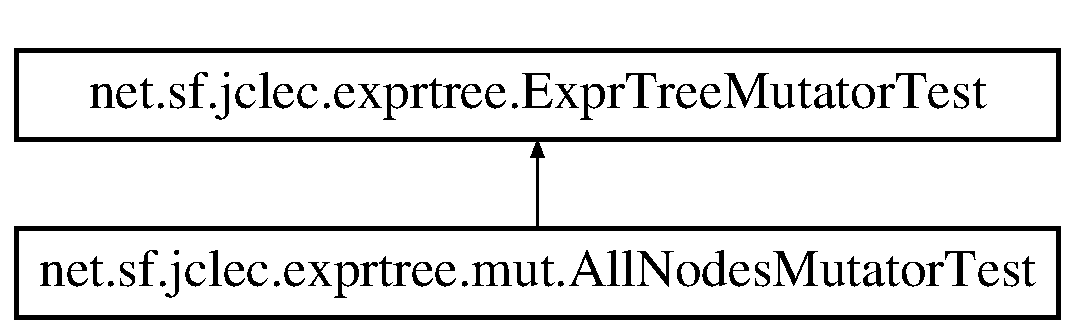
\includegraphics[height=2.000000cm]{classnet_1_1sf_1_1jclec_1_1exprtree_1_1mut_1_1_all_nodes_mutator_test}
\end{center}
\end{figure}
\subsection*{Public Member Functions}
\begin{DoxyCompactItemize}
\item 
\hyperlink{classnet_1_1sf_1_1jclec_1_1exprtree_1_1mut_1_1_all_nodes_mutator_test_ae668b8b26ae1a93a5d0a61073d5d0b84}{All\-Nodes\-Mutator\-Test} (String name)
\end{DoxyCompactItemize}


\subsection{Detailed Description}
Unit tests for \hyperlink{classnet_1_1sf_1_1jclec_1_1exprtree_1_1mut_1_1_all_nodes_mutator_test}{All\-Nodes\-Mutator\-Test}.

\begin{DoxyAuthor}{Author}
Amelia Zafra -\/ Sebastian Ventura 
\end{DoxyAuthor}


\subsection{Constructor \& Destructor Documentation}
\hypertarget{classnet_1_1sf_1_1jclec_1_1exprtree_1_1mut_1_1_all_nodes_mutator_test_ae668b8b26ae1a93a5d0a61073d5d0b84}{\index{net\-::sf\-::jclec\-::exprtree\-::mut\-::\-All\-Nodes\-Mutator\-Test@{net\-::sf\-::jclec\-::exprtree\-::mut\-::\-All\-Nodes\-Mutator\-Test}!All\-Nodes\-Mutator\-Test@{All\-Nodes\-Mutator\-Test}}
\index{All\-Nodes\-Mutator\-Test@{All\-Nodes\-Mutator\-Test}!net::sf::jclec::exprtree::mut::AllNodesMutatorTest@{net\-::sf\-::jclec\-::exprtree\-::mut\-::\-All\-Nodes\-Mutator\-Test}}
\subsubsection[{All\-Nodes\-Mutator\-Test}]{\setlength{\rightskip}{0pt plus 5cm}net.\-sf.\-jclec.\-exprtree.\-mut.\-All\-Nodes\-Mutator\-Test.\-All\-Nodes\-Mutator\-Test (
\begin{DoxyParamCaption}
\item[{String}]{name}
\end{DoxyParamCaption}
)}}\label{classnet_1_1sf_1_1jclec_1_1exprtree_1_1mut_1_1_all_nodes_mutator_test_ae668b8b26ae1a93a5d0a61073d5d0b84}
Default constructor. 

The documentation for this class was generated from the following file\-:\begin{DoxyCompactItemize}
\item 
src/test/java/net/sf/jclec/exprtree/mut/All\-Nodes\-Mutator\-Test.\-java\end{DoxyCompactItemize}

\hypertarget{classnet_1_1sf_1_1jclec_1_1exprtree_1_1fun_1_1_argument_3_01_e_01_4}{\section{net.\-sf.\-jclec.\-exprtree.\-fun.\-Argument$<$ E $>$ Class Reference}
\label{classnet_1_1sf_1_1jclec_1_1exprtree_1_1fun_1_1_argument_3_01_e_01_4}\index{net.\-sf.\-jclec.\-exprtree.\-fun.\-Argument$<$ E $>$@{net.\-sf.\-jclec.\-exprtree.\-fun.\-Argument$<$ E $>$}}
}
Inheritance diagram for net.\-sf.\-jclec.\-exprtree.\-fun.\-Argument$<$ E $>$\-:\begin{figure}[H]
\begin{center}
\leavevmode
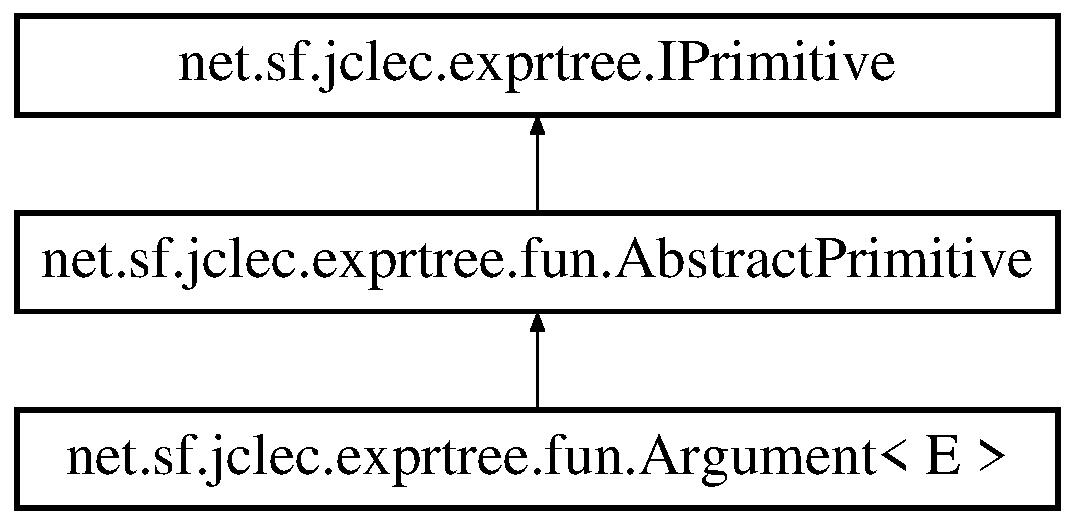
\includegraphics[height=3.000000cm]{classnet_1_1sf_1_1jclec_1_1exprtree_1_1fun_1_1_argument_3_01_e_01_4}
\end{center}
\end{figure}
\subsection*{Protected Member Functions}
\begin{DoxyCompactItemize}
\item 
final void \hyperlink{classnet_1_1sf_1_1jclec_1_1exprtree_1_1fun_1_1_argument_3_01_e_01_4_a8961f8dae241232cc573ba53278f3b73}{evaluate} (\hyperlink{classnet_1_1sf_1_1jclec_1_1exprtree_1_1fun_1_1_expr_tree_function}{Expr\-Tree\-Function} context)
\end{DoxyCompactItemize}
\subsection*{Protected Attributes}
\begin{DoxyCompactItemize}
\item 
int \hyperlink{classnet_1_1sf_1_1jclec_1_1exprtree_1_1fun_1_1_argument_3_01_e_01_4_ab11c82b51e183d019a0d916c2841e5cc}{argindex}
\end{DoxyCompactItemize}
\subsection*{Additional Inherited Members}


\subsection{Detailed Description}
Argument. This class represents generically an argument in the arguments pool.

\begin{DoxyAuthor}{Author}
Sebastian Ventura
\end{DoxyAuthor}

\begin{DoxyParams}{Parameters}
{\em $<$\-E$>$} & Argument type \\
\hline
\end{DoxyParams}


\subsection{Member Function Documentation}
\hypertarget{classnet_1_1sf_1_1jclec_1_1exprtree_1_1fun_1_1_argument_3_01_e_01_4_a8961f8dae241232cc573ba53278f3b73}{\index{net\-::sf\-::jclec\-::exprtree\-::fun\-::\-Argument$<$ E $>$@{net\-::sf\-::jclec\-::exprtree\-::fun\-::\-Argument$<$ E $>$}!evaluate@{evaluate}}
\index{evaluate@{evaluate}!net::sf::jclec::exprtree::fun::Argument< E >@{net\-::sf\-::jclec\-::exprtree\-::fun\-::\-Argument$<$ E $>$}}
\subsubsection[{evaluate}]{\setlength{\rightskip}{0pt plus 5cm}final void net.\-sf.\-jclec.\-exprtree.\-fun.\-Argument$<$ E $>$.evaluate (
\begin{DoxyParamCaption}
\item[{{\bf Expr\-Tree\-Function}}]{context}
\end{DoxyParamCaption}
)\hspace{0.3cm}{\ttfamily [protected]}, {\ttfamily [virtual]}}}\label{classnet_1_1sf_1_1jclec_1_1exprtree_1_1fun_1_1_argument_3_01_e_01_4_a8961f8dae241232cc573ba53278f3b73}
Evaluate this primitive.


\begin{DoxyParams}{Parameters}
{\em context} & Execution context \\
\hline
\end{DoxyParams}


Implements \hyperlink{classnet_1_1sf_1_1jclec_1_1exprtree_1_1fun_1_1_abstract_primitive_aab695f920997a9f1d873ab9b6f3ca246}{net.\-sf.\-jclec.\-exprtree.\-fun.\-Abstract\-Primitive}.



\subsection{Member Data Documentation}
\hypertarget{classnet_1_1sf_1_1jclec_1_1exprtree_1_1fun_1_1_argument_3_01_e_01_4_ab11c82b51e183d019a0d916c2841e5cc}{\index{net\-::sf\-::jclec\-::exprtree\-::fun\-::\-Argument$<$ E $>$@{net\-::sf\-::jclec\-::exprtree\-::fun\-::\-Argument$<$ E $>$}!argindex@{argindex}}
\index{argindex@{argindex}!net::sf::jclec::exprtree::fun::Argument< E >@{net\-::sf\-::jclec\-::exprtree\-::fun\-::\-Argument$<$ E $>$}}
\subsubsection[{argindex}]{\setlength{\rightskip}{0pt plus 5cm}int net.\-sf.\-jclec.\-exprtree.\-fun.\-Argument$<$ E $>$.argindex\hspace{0.3cm}{\ttfamily [protected]}}}\label{classnet_1_1sf_1_1jclec_1_1exprtree_1_1fun_1_1_argument_3_01_e_01_4_ab11c82b51e183d019a0d916c2841e5cc}
Argument index 

The documentation for this class was generated from the following file\-:\begin{DoxyCompactItemize}
\item 
src/main/java/net/sf/jclec/exprtree/fun/Argument.\-java\end{DoxyCompactItemize}

\hypertarget{classnet_1_1sf_1_1jclec_1_1realarray_1_1rec_1_1_arithmetic_crossover}{\section{net.\-sf.\-jclec.\-realarray.\-rec.\-Arithmetic\-Crossover Class Reference}
\label{classnet_1_1sf_1_1jclec_1_1realarray_1_1rec_1_1_arithmetic_crossover}\index{net.\-sf.\-jclec.\-realarray.\-rec.\-Arithmetic\-Crossover@{net.\-sf.\-jclec.\-realarray.\-rec.\-Arithmetic\-Crossover}}
}


Inherits net.\-sf.\-jclec.\-realarray.\-rec.\-Uniform\-Crossover2x2.

\subsection*{Public Member Functions}
\begin{DoxyCompactItemize}
\item 
\hyperlink{classnet_1_1sf_1_1jclec_1_1realarray_1_1rec_1_1_arithmetic_crossover_ae538fa888a52648f4a171128303f9b44}{Arithmetic\-Crossover} ()
\item 
double \hyperlink{classnet_1_1sf_1_1jclec_1_1realarray_1_1rec_1_1_arithmetic_crossover_a87e47236383dd187320787e50b151bdf}{get\-Lambda} ()
\item 
void \hyperlink{classnet_1_1sf_1_1jclec_1_1realarray_1_1rec_1_1_arithmetic_crossover_af835e6d90325c473bd4736059e328b48}{set\-Lambda} (double \hyperlink{classnet_1_1sf_1_1jclec_1_1realarray_1_1rec_1_1_arithmetic_crossover_ab29f2d1172e5106746b24cc9fa9e1c24}{lambda})
\item 
void \hyperlink{classnet_1_1sf_1_1jclec_1_1realarray_1_1rec_1_1_arithmetic_crossover_a7f0403004c9f0c01a9ce54c544a38c5d}{configure} (Configuration settings)
\end{DoxyCompactItemize}
\subsection*{Protected Member Functions}
\begin{DoxyCompactItemize}
\item 
double \hyperlink{classnet_1_1sf_1_1jclec_1_1realarray_1_1rec_1_1_arithmetic_crossover_a0d1440dac8411c5d0140e7754821ff78}{default\-Locus\-Rec\-Prob} ()
\end{DoxyCompactItemize}
\subsection*{Protected Attributes}
\begin{DoxyCompactItemize}
\item 
double \hyperlink{classnet_1_1sf_1_1jclec_1_1realarray_1_1rec_1_1_arithmetic_crossover_ab29f2d1172e5106746b24cc9fa9e1c24}{lambda}
\end{DoxyCompactItemize}


\subsection{Detailed Description}
Arithmetic crossover for \hyperlink{classnet_1_1sf_1_1jclec_1_1realarray_1_1_real_array_individual}{Real\-Array\-Individual} and its subclasses

\begin{DoxyAuthor}{Author}
Alberto Lamarca 

Sebastian Ventura 
\end{DoxyAuthor}


\subsection{Constructor \& Destructor Documentation}
\hypertarget{classnet_1_1sf_1_1jclec_1_1realarray_1_1rec_1_1_arithmetic_crossover_ae538fa888a52648f4a171128303f9b44}{\index{net\-::sf\-::jclec\-::realarray\-::rec\-::\-Arithmetic\-Crossover@{net\-::sf\-::jclec\-::realarray\-::rec\-::\-Arithmetic\-Crossover}!Arithmetic\-Crossover@{Arithmetic\-Crossover}}
\index{Arithmetic\-Crossover@{Arithmetic\-Crossover}!net::sf::jclec::realarray::rec::ArithmeticCrossover@{net\-::sf\-::jclec\-::realarray\-::rec\-::\-Arithmetic\-Crossover}}
\subsubsection[{Arithmetic\-Crossover}]{\setlength{\rightskip}{0pt plus 5cm}net.\-sf.\-jclec.\-realarray.\-rec.\-Arithmetic\-Crossover.\-Arithmetic\-Crossover (
\begin{DoxyParamCaption}
{}
\end{DoxyParamCaption}
)}}\label{classnet_1_1sf_1_1jclec_1_1realarray_1_1rec_1_1_arithmetic_crossover_ae538fa888a52648f4a171128303f9b44}
Empty constructor 

\subsection{Member Function Documentation}
\hypertarget{classnet_1_1sf_1_1jclec_1_1realarray_1_1rec_1_1_arithmetic_crossover_a7f0403004c9f0c01a9ce54c544a38c5d}{\index{net\-::sf\-::jclec\-::realarray\-::rec\-::\-Arithmetic\-Crossover@{net\-::sf\-::jclec\-::realarray\-::rec\-::\-Arithmetic\-Crossover}!configure@{configure}}
\index{configure@{configure}!net::sf::jclec::realarray::rec::ArithmeticCrossover@{net\-::sf\-::jclec\-::realarray\-::rec\-::\-Arithmetic\-Crossover}}
\subsubsection[{configure}]{\setlength{\rightskip}{0pt plus 5cm}void net.\-sf.\-jclec.\-realarray.\-rec.\-Arithmetic\-Crossover.\-configure (
\begin{DoxyParamCaption}
\item[{Configuration}]{settings}
\end{DoxyParamCaption}
)}}\label{classnet_1_1sf_1_1jclec_1_1realarray_1_1rec_1_1_arithmetic_crossover_a7f0403004c9f0c01a9ce54c544a38c5d}
Configuration method.


\begin{DoxyParams}{Parameters}
{\em settings} & Configuration settings \\
\hline
\end{DoxyParams}


Implements \hyperlink{interfacenet_1_1sf_1_1jclec_1_1_i_configure_add31a65a04d148c690a956fbbad6987c}{net.\-sf.\-jclec.\-I\-Configure}.

\hypertarget{classnet_1_1sf_1_1jclec_1_1realarray_1_1rec_1_1_arithmetic_crossover_a0d1440dac8411c5d0140e7754821ff78}{\index{net\-::sf\-::jclec\-::realarray\-::rec\-::\-Arithmetic\-Crossover@{net\-::sf\-::jclec\-::realarray\-::rec\-::\-Arithmetic\-Crossover}!default\-Locus\-Rec\-Prob@{default\-Locus\-Rec\-Prob}}
\index{default\-Locus\-Rec\-Prob@{default\-Locus\-Rec\-Prob}!net::sf::jclec::realarray::rec::ArithmeticCrossover@{net\-::sf\-::jclec\-::realarray\-::rec\-::\-Arithmetic\-Crossover}}
\subsubsection[{default\-Locus\-Rec\-Prob}]{\setlength{\rightskip}{0pt plus 5cm}double net.\-sf.\-jclec.\-realarray.\-rec.\-Arithmetic\-Crossover.\-default\-Locus\-Rec\-Prob (
\begin{DoxyParamCaption}
{}
\end{DoxyParamCaption}
)\hspace{0.3cm}{\ttfamily [protected]}, {\ttfamily [virtual]}}}\label{classnet_1_1sf_1_1jclec_1_1realarray_1_1rec_1_1_arithmetic_crossover_a0d1440dac8411c5d0140e7754821ff78}
Get default value for this parameter. 

Implements \hyperlink{classnet_1_1sf_1_1jclec_1_1realarray_1_1_uniform_crossover_ac427b4ae11cf8b9495625005fe5ec575}{net.\-sf.\-jclec.\-realarray.\-Uniform\-Crossover}.

\hypertarget{classnet_1_1sf_1_1jclec_1_1realarray_1_1rec_1_1_arithmetic_crossover_a87e47236383dd187320787e50b151bdf}{\index{net\-::sf\-::jclec\-::realarray\-::rec\-::\-Arithmetic\-Crossover@{net\-::sf\-::jclec\-::realarray\-::rec\-::\-Arithmetic\-Crossover}!get\-Lambda@{get\-Lambda}}
\index{get\-Lambda@{get\-Lambda}!net::sf::jclec::realarray::rec::ArithmeticCrossover@{net\-::sf\-::jclec\-::realarray\-::rec\-::\-Arithmetic\-Crossover}}
\subsubsection[{get\-Lambda}]{\setlength{\rightskip}{0pt plus 5cm}double net.\-sf.\-jclec.\-realarray.\-rec.\-Arithmetic\-Crossover.\-get\-Lambda (
\begin{DoxyParamCaption}
{}
\end{DoxyParamCaption}
)}}\label{classnet_1_1sf_1_1jclec_1_1realarray_1_1rec_1_1_arithmetic_crossover_a87e47236383dd187320787e50b151bdf}
\begin{DoxyReturn}{Returns}
Returns the lambda. 
\end{DoxyReturn}
\hypertarget{classnet_1_1sf_1_1jclec_1_1realarray_1_1rec_1_1_arithmetic_crossover_af835e6d90325c473bd4736059e328b48}{\index{net\-::sf\-::jclec\-::realarray\-::rec\-::\-Arithmetic\-Crossover@{net\-::sf\-::jclec\-::realarray\-::rec\-::\-Arithmetic\-Crossover}!set\-Lambda@{set\-Lambda}}
\index{set\-Lambda@{set\-Lambda}!net::sf::jclec::realarray::rec::ArithmeticCrossover@{net\-::sf\-::jclec\-::realarray\-::rec\-::\-Arithmetic\-Crossover}}
\subsubsection[{set\-Lambda}]{\setlength{\rightskip}{0pt plus 5cm}void net.\-sf.\-jclec.\-realarray.\-rec.\-Arithmetic\-Crossover.\-set\-Lambda (
\begin{DoxyParamCaption}
\item[{double}]{lambda}
\end{DoxyParamCaption}
)}}\label{classnet_1_1sf_1_1jclec_1_1realarray_1_1rec_1_1_arithmetic_crossover_af835e6d90325c473bd4736059e328b48}

\begin{DoxyParams}{Parameters}
{\em lambda} & The lambda to set. \\
\hline
\end{DoxyParams}


\subsection{Member Data Documentation}
\hypertarget{classnet_1_1sf_1_1jclec_1_1realarray_1_1rec_1_1_arithmetic_crossover_ab29f2d1172e5106746b24cc9fa9e1c24}{\index{net\-::sf\-::jclec\-::realarray\-::rec\-::\-Arithmetic\-Crossover@{net\-::sf\-::jclec\-::realarray\-::rec\-::\-Arithmetic\-Crossover}!lambda@{lambda}}
\index{lambda@{lambda}!net::sf::jclec::realarray::rec::ArithmeticCrossover@{net\-::sf\-::jclec\-::realarray\-::rec\-::\-Arithmetic\-Crossover}}
\subsubsection[{lambda}]{\setlength{\rightskip}{0pt plus 5cm}double net.\-sf.\-jclec.\-realarray.\-rec.\-Arithmetic\-Crossover.\-lambda\hspace{0.3cm}{\ttfamily [protected]}}}\label{classnet_1_1sf_1_1jclec_1_1realarray_1_1rec_1_1_arithmetic_crossover_ab29f2d1172e5106746b24cc9fa9e1c24}
Lambda parameter 

The documentation for this class was generated from the following file\-:\begin{DoxyCompactItemize}
\item 
src/main/java/net/sf/jclec/realarray/rec/Arithmetic\-Crossover.\-java\end{DoxyCompactItemize}

\hypertarget{classnet_1_1sf_1_1jclec_1_1selector_1_1_betters_selector}{\section{net.\-sf.\-jclec.\-selector.\-Betters\-Selector Class Reference}
\label{classnet_1_1sf_1_1jclec_1_1selector_1_1_betters_selector}\index{net.\-sf.\-jclec.\-selector.\-Betters\-Selector@{net.\-sf.\-jclec.\-selector.\-Betters\-Selector}}
}
Inheritance diagram for net.\-sf.\-jclec.\-selector.\-Betters\-Selector\-:\begin{figure}[H]
\begin{center}
\leavevmode
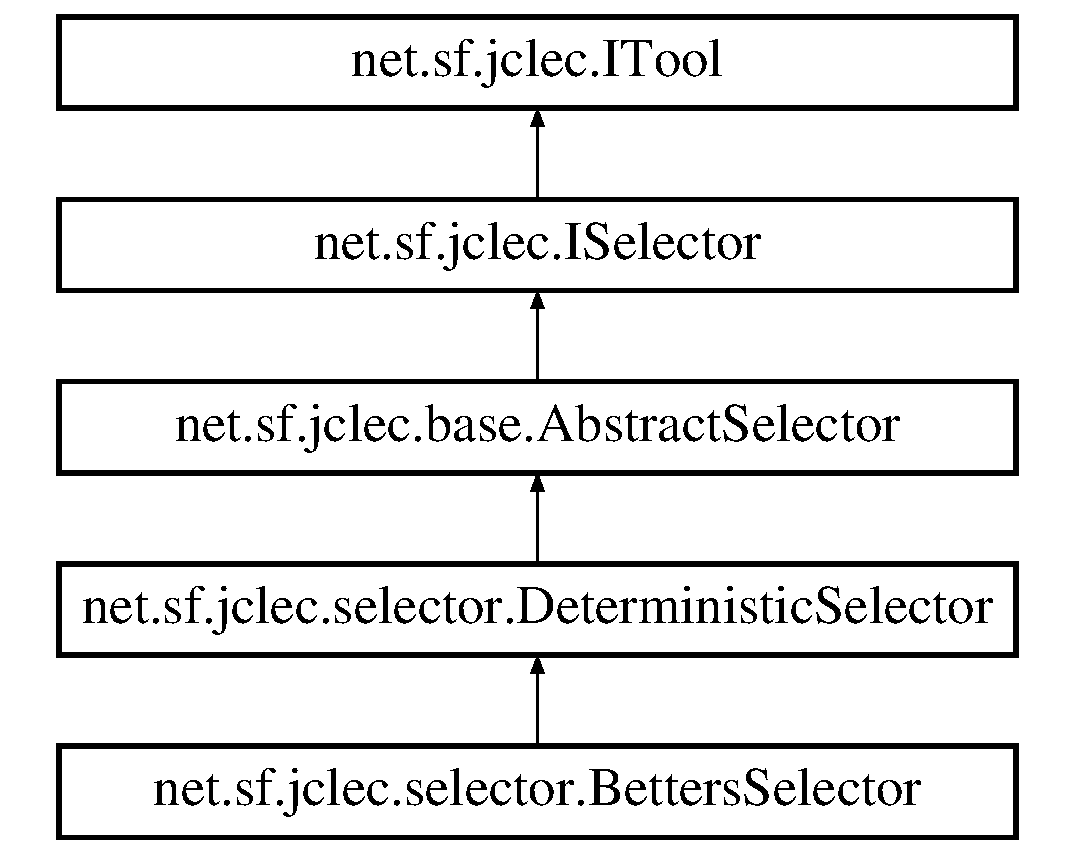
\includegraphics[height=5.000000cm]{classnet_1_1sf_1_1jclec_1_1selector_1_1_betters_selector}
\end{center}
\end{figure}
\subsection*{Public Member Functions}
\begin{DoxyCompactItemize}
\item 
\hyperlink{classnet_1_1sf_1_1jclec_1_1selector_1_1_betters_selector_a539ecdfd09de70e7f71d43a92506e5bc}{Betters\-Selector} ()
\end{DoxyCompactItemize}
\subsection*{Protected Member Functions}
\begin{DoxyCompactItemize}
\item 
void \hyperlink{classnet_1_1sf_1_1jclec_1_1selector_1_1_betters_selector_a6e1bf12a092b5d3cc1ac8010aa032480}{prepare\-Selection} ()
\item 
\hyperlink{interfacenet_1_1sf_1_1jclec_1_1_i_individual}{I\-Individual} \hyperlink{classnet_1_1sf_1_1jclec_1_1selector_1_1_betters_selector_aafc05c782c8e38e6c39130fc3c1fa1a3}{select\-Next} ()
\end{DoxyCompactItemize}
\subsection*{Protected Attributes}
\begin{DoxyCompactItemize}
\item 
transient Comparator$<$ \hyperlink{interfacenet_1_1sf_1_1jclec_1_1_i_individual}{I\-Individual} $>$ \hyperlink{classnet_1_1sf_1_1jclec_1_1selector_1_1_betters_selector_a2fb4bd969e30aba010fdc77798fad6a4}{individuals\-Comparator}
\item 
transient Comparator$<$ \hyperlink{interfacenet_1_1sf_1_1jclec_1_1_i_fitness}{I\-Fitness} $>$ \hyperlink{classnet_1_1sf_1_1jclec_1_1selector_1_1_betters_selector_a6841f51f9dcb6e22c7e8c3875b324c34}{fitness\-Comparator}
\item 
transient Array\-List$<$ \hyperlink{interfacenet_1_1sf_1_1jclec_1_1_i_individual}{I\-Individual} $>$ \hyperlink{classnet_1_1sf_1_1jclec_1_1selector_1_1_betters_selector_ab1d403d53ac1f1cbb3d0ddd51fd0e160}{aux\-List} = new Array\-List$<$\hyperlink{interfacenet_1_1sf_1_1jclec_1_1_i_individual}{I\-Individual}$>$ ()
\end{DoxyCompactItemize}


\subsection{Detailed Description}
Better individuals selector.

\begin{DoxyAuthor}{Author}
Sebastian Ventura 
\end{DoxyAuthor}


\subsection{Constructor \& Destructor Documentation}
\hypertarget{classnet_1_1sf_1_1jclec_1_1selector_1_1_betters_selector_a539ecdfd09de70e7f71d43a92506e5bc}{\index{net\-::sf\-::jclec\-::selector\-::\-Betters\-Selector@{net\-::sf\-::jclec\-::selector\-::\-Betters\-Selector}!Betters\-Selector@{Betters\-Selector}}
\index{Betters\-Selector@{Betters\-Selector}!net::sf::jclec::selector::BettersSelector@{net\-::sf\-::jclec\-::selector\-::\-Betters\-Selector}}
\subsubsection[{Betters\-Selector}]{\setlength{\rightskip}{0pt plus 5cm}net.\-sf.\-jclec.\-selector.\-Betters\-Selector.\-Betters\-Selector (
\begin{DoxyParamCaption}
{}
\end{DoxyParamCaption}
)}}\label{classnet_1_1sf_1_1jclec_1_1selector_1_1_betters_selector_a539ecdfd09de70e7f71d43a92506e5bc}
Empty constructor. 

\subsection{Member Function Documentation}
\hypertarget{classnet_1_1sf_1_1jclec_1_1selector_1_1_betters_selector_a6e1bf12a092b5d3cc1ac8010aa032480}{\index{net\-::sf\-::jclec\-::selector\-::\-Betters\-Selector@{net\-::sf\-::jclec\-::selector\-::\-Betters\-Selector}!prepare\-Selection@{prepare\-Selection}}
\index{prepare\-Selection@{prepare\-Selection}!net::sf::jclec::selector::BettersSelector@{net\-::sf\-::jclec\-::selector\-::\-Betters\-Selector}}
\subsubsection[{prepare\-Selection}]{\setlength{\rightskip}{0pt plus 5cm}void net.\-sf.\-jclec.\-selector.\-Betters\-Selector.\-prepare\-Selection (
\begin{DoxyParamCaption}
{}
\end{DoxyParamCaption}
)\hspace{0.3cm}{\ttfamily [protected]}, {\ttfamily [virtual]}}}\label{classnet_1_1sf_1_1jclec_1_1selector_1_1_betters_selector_a6e1bf12a092b5d3cc1ac8010aa032480}
Prepare selection consists on take fitnesses comparator (to compare individuals by fitness). Then, copy all source inds in a temporary list

Prepare the selection process. 

Implements \hyperlink{classnet_1_1sf_1_1jclec_1_1base_1_1_abstract_selector_a0c5d9cb96fef9786e272b9edd811111e}{net.\-sf.\-jclec.\-base.\-Abstract\-Selector}.

\hypertarget{classnet_1_1sf_1_1jclec_1_1selector_1_1_betters_selector_aafc05c782c8e38e6c39130fc3c1fa1a3}{\index{net\-::sf\-::jclec\-::selector\-::\-Betters\-Selector@{net\-::sf\-::jclec\-::selector\-::\-Betters\-Selector}!select\-Next@{select\-Next}}
\index{select\-Next@{select\-Next}!net::sf::jclec::selector::BettersSelector@{net\-::sf\-::jclec\-::selector\-::\-Betters\-Selector}}
\subsubsection[{select\-Next}]{\setlength{\rightskip}{0pt plus 5cm}{\bf I\-Individual} net.\-sf.\-jclec.\-selector.\-Betters\-Selector.\-select\-Next (
\begin{DoxyParamCaption}
{}
\end{DoxyParamCaption}
)\hspace{0.3cm}{\ttfamily [protected]}, {\ttfamily [virtual]}}}\label{classnet_1_1sf_1_1jclec_1_1selector_1_1_betters_selector_aafc05c782c8e38e6c39130fc3c1fa1a3}
This method take best individual in temporary list, then remove and return it.

Selects an individual (in the context of a selection process).

\begin{DoxyReturn}{Returns}
Selected individual
\end{DoxyReturn}
 

Implements \hyperlink{classnet_1_1sf_1_1jclec_1_1base_1_1_abstract_selector_aa2ccb539c608db9c14ebbc763807b95a}{net.\-sf.\-jclec.\-base.\-Abstract\-Selector}.



\subsection{Member Data Documentation}
\hypertarget{classnet_1_1sf_1_1jclec_1_1selector_1_1_betters_selector_ab1d403d53ac1f1cbb3d0ddd51fd0e160}{\index{net\-::sf\-::jclec\-::selector\-::\-Betters\-Selector@{net\-::sf\-::jclec\-::selector\-::\-Betters\-Selector}!aux\-List@{aux\-List}}
\index{aux\-List@{aux\-List}!net::sf::jclec::selector::BettersSelector@{net\-::sf\-::jclec\-::selector\-::\-Betters\-Selector}}
\subsubsection[{aux\-List}]{\setlength{\rightskip}{0pt plus 5cm}transient Array\-List$<${\bf I\-Individual}$>$ net.\-sf.\-jclec.\-selector.\-Betters\-Selector.\-aux\-List = new Array\-List$<${\bf I\-Individual}$>$ ()\hspace{0.3cm}{\ttfamily [protected]}}}\label{classnet_1_1sf_1_1jclec_1_1selector_1_1_betters_selector_ab1d403d53ac1f1cbb3d0ddd51fd0e160}
Auxiliary list \hypertarget{classnet_1_1sf_1_1jclec_1_1selector_1_1_betters_selector_a6841f51f9dcb6e22c7e8c3875b324c34}{\index{net\-::sf\-::jclec\-::selector\-::\-Betters\-Selector@{net\-::sf\-::jclec\-::selector\-::\-Betters\-Selector}!fitness\-Comparator@{fitness\-Comparator}}
\index{fitness\-Comparator@{fitness\-Comparator}!net::sf::jclec::selector::BettersSelector@{net\-::sf\-::jclec\-::selector\-::\-Betters\-Selector}}
\subsubsection[{fitness\-Comparator}]{\setlength{\rightskip}{0pt plus 5cm}transient Comparator$<${\bf I\-Fitness}$>$ net.\-sf.\-jclec.\-selector.\-Betters\-Selector.\-fitness\-Comparator\hspace{0.3cm}{\ttfamily [protected]}}}\label{classnet_1_1sf_1_1jclec_1_1selector_1_1_betters_selector_a6841f51f9dcb6e22c7e8c3875b324c34}
Fitness comparator (taken from context) \hypertarget{classnet_1_1sf_1_1jclec_1_1selector_1_1_betters_selector_a2fb4bd969e30aba010fdc77798fad6a4}{\index{net\-::sf\-::jclec\-::selector\-::\-Betters\-Selector@{net\-::sf\-::jclec\-::selector\-::\-Betters\-Selector}!individuals\-Comparator@{individuals\-Comparator}}
\index{individuals\-Comparator@{individuals\-Comparator}!net::sf::jclec::selector::BettersSelector@{net\-::sf\-::jclec\-::selector\-::\-Betters\-Selector}}
\subsubsection[{individuals\-Comparator}]{\setlength{\rightskip}{0pt plus 5cm}transient Comparator$<${\bf I\-Individual}$>$ net.\-sf.\-jclec.\-selector.\-Betters\-Selector.\-individuals\-Comparator\hspace{0.3cm}{\ttfamily [protected]}}}\label{classnet_1_1sf_1_1jclec_1_1selector_1_1_betters_selector_a2fb4bd969e30aba010fdc77798fad6a4}
{\bfseries Initial value\-:}
\begin{DoxyCode}
=  
        \textcolor{keyword}{new} Comparator<IIndividual> () 
        \{
            
        
            \textcolor{keyword}{public} \textcolor{keywordtype}{int} compare(IIndividual arg0, IIndividual arg1) \{
                \textcolor{keywordflow}{return} fitnessComparator.compare(arg0.getFitness(), arg1.getFitness());
            \}
        \}
\end{DoxyCode}
Compare individuals 

The documentation for this class was generated from the following file\-:\begin{DoxyCompactItemize}
\item 
src/main/java/net/sf/jclec/selector/Betters\-Selector.\-java\end{DoxyCompactItemize}

\hypertarget{classnet_1_1sf_1_1jclec_1_1binarray_1_1_bin_array_creator}{\section{net.\-sf.\-jclec.\-binarray.\-Bin\-Array\-Creator Class Reference}
\label{classnet_1_1sf_1_1jclec_1_1binarray_1_1_bin_array_creator}\index{net.\-sf.\-jclec.\-binarray.\-Bin\-Array\-Creator@{net.\-sf.\-jclec.\-binarray.\-Bin\-Array\-Creator}}
}
Inheritance diagram for net.\-sf.\-jclec.\-binarray.\-Bin\-Array\-Creator\-:\begin{figure}[H]
\begin{center}
\leavevmode
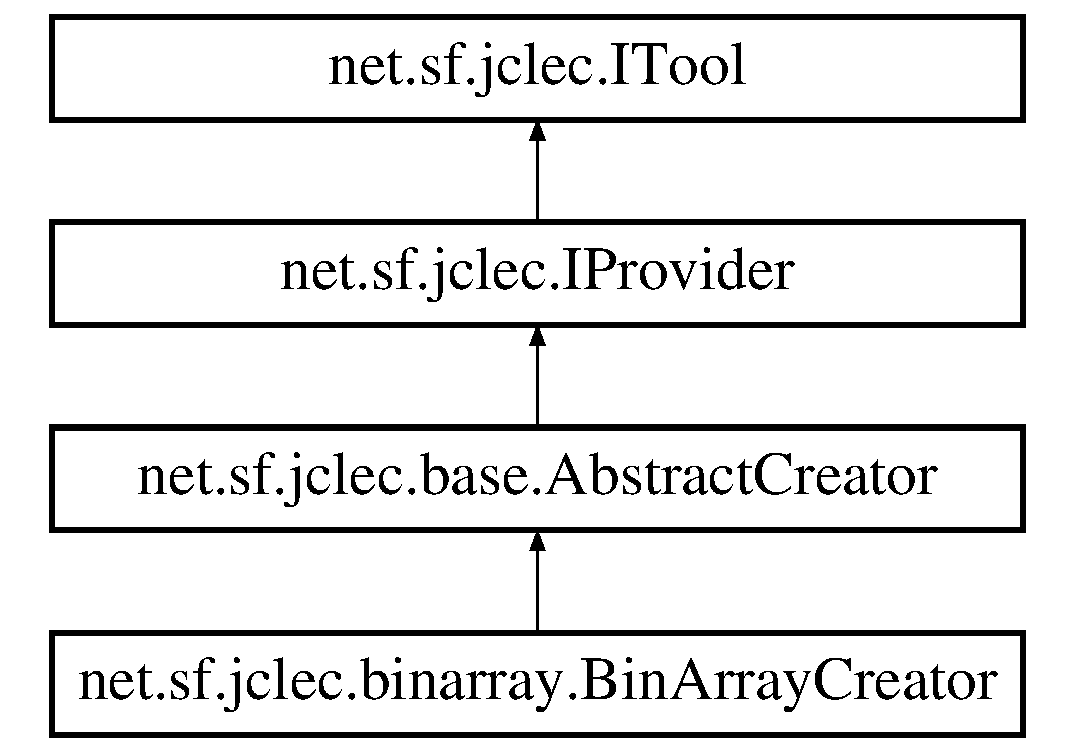
\includegraphics[height=4.000000cm]{classnet_1_1sf_1_1jclec_1_1binarray_1_1_bin_array_creator}
\end{center}
\end{figure}
\subsection*{Public Member Functions}
\begin{DoxyCompactItemize}
\item 
boolean \hyperlink{classnet_1_1sf_1_1jclec_1_1binarray_1_1_bin_array_creator_a2190fa73d1e2211dcf783d3b6a78f929}{equals} (Object other)
\end{DoxyCompactItemize}
\subsection*{Protected Member Functions}
\begin{DoxyCompactItemize}
\item 
void \hyperlink{classnet_1_1sf_1_1jclec_1_1binarray_1_1_bin_array_creator_a51d110d716e41756a37c508a5d92b478}{prepare\-Creation} ()
\item 
void \hyperlink{classnet_1_1sf_1_1jclec_1_1binarray_1_1_bin_array_creator_aff93b467bf15009d84d97e5427398985}{create\-Next} ()
\end{DoxyCompactItemize}
\subsection*{Protected Attributes}
\begin{DoxyCompactItemize}
\item 
transient \hyperlink{classnet_1_1sf_1_1jclec_1_1binarray_1_1_bin_array_species}{Bin\-Array\-Species} \hyperlink{classnet_1_1sf_1_1jclec_1_1binarray_1_1_bin_array_creator_a166ddebeaa80af211d1bb7c87786d7e7}{species}
\item 
transient byte\mbox{[}$\,$\mbox{]} \hyperlink{classnet_1_1sf_1_1jclec_1_1binarray_1_1_bin_array_creator_aaa529b1abd5a153760b138335d258926}{schema}
\end{DoxyCompactItemize}


\subsection{Detailed Description}
Creation of \hyperlink{classnet_1_1sf_1_1jclec_1_1binarray_1_1_bin_array_individual}{Bin\-Array\-Individual} (and subclasses).

\begin{DoxyAuthor}{Author}
Sebastian Ventura 
\end{DoxyAuthor}


\subsection{Member Function Documentation}
\hypertarget{classnet_1_1sf_1_1jclec_1_1binarray_1_1_bin_array_creator_aff93b467bf15009d84d97e5427398985}{\index{net\-::sf\-::jclec\-::binarray\-::\-Bin\-Array\-Creator@{net\-::sf\-::jclec\-::binarray\-::\-Bin\-Array\-Creator}!create\-Next@{create\-Next}}
\index{create\-Next@{create\-Next}!net::sf::jclec::binarray::BinArrayCreator@{net\-::sf\-::jclec\-::binarray\-::\-Bin\-Array\-Creator}}
\subsubsection[{create\-Next}]{\setlength{\rightskip}{0pt plus 5cm}void net.\-sf.\-jclec.\-binarray.\-Bin\-Array\-Creator.\-create\-Next (
\begin{DoxyParamCaption}
{}
\end{DoxyParamCaption}
)\hspace{0.3cm}{\ttfamily [protected]}, {\ttfamily [virtual]}}}\label{classnet_1_1sf_1_1jclec_1_1binarray_1_1_bin_array_creator_aff93b467bf15009d84d97e5427398985}
Creation method.


\begin{DoxyParams}{Parameters}
{\em ind} & Individual to create\\
\hline
\end{DoxyParams}
\begin{DoxyReturn}{Returns}
New individual
\end{DoxyReturn}
 

Implements \hyperlink{classnet_1_1sf_1_1jclec_1_1base_1_1_abstract_creator_aee6bcace778e7421fc5c07e1a4f6fed9}{net.\-sf.\-jclec.\-base.\-Abstract\-Creator}.

\hypertarget{classnet_1_1sf_1_1jclec_1_1binarray_1_1_bin_array_creator_a2190fa73d1e2211dcf783d3b6a78f929}{\index{net\-::sf\-::jclec\-::binarray\-::\-Bin\-Array\-Creator@{net\-::sf\-::jclec\-::binarray\-::\-Bin\-Array\-Creator}!equals@{equals}}
\index{equals@{equals}!net::sf::jclec::binarray::BinArrayCreator@{net\-::sf\-::jclec\-::binarray\-::\-Bin\-Array\-Creator}}
\subsubsection[{equals}]{\setlength{\rightskip}{0pt plus 5cm}boolean net.\-sf.\-jclec.\-binarray.\-Bin\-Array\-Creator.\-equals (
\begin{DoxyParamCaption}
\item[{Object}]{other}
\end{DoxyParamCaption}
)}}\label{classnet_1_1sf_1_1jclec_1_1binarray_1_1_bin_array_creator_a2190fa73d1e2211dcf783d3b6a78f929}
\hypertarget{classnet_1_1sf_1_1jclec_1_1binarray_1_1_bin_array_creator_a51d110d716e41756a37c508a5d92b478}{\index{net\-::sf\-::jclec\-::binarray\-::\-Bin\-Array\-Creator@{net\-::sf\-::jclec\-::binarray\-::\-Bin\-Array\-Creator}!prepare\-Creation@{prepare\-Creation}}
\index{prepare\-Creation@{prepare\-Creation}!net::sf::jclec::binarray::BinArrayCreator@{net\-::sf\-::jclec\-::binarray\-::\-Bin\-Array\-Creator}}
\subsubsection[{prepare\-Creation}]{\setlength{\rightskip}{0pt plus 5cm}void net.\-sf.\-jclec.\-binarray.\-Bin\-Array\-Creator.\-prepare\-Creation (
\begin{DoxyParamCaption}
{}
\end{DoxyParamCaption}
)\hspace{0.3cm}{\ttfamily [protected]}, {\ttfamily [virtual]}}}\label{classnet_1_1sf_1_1jclec_1_1binarray_1_1_bin_array_creator_a51d110d716e41756a37c508a5d92b478}
Prepare creation process. 

Implements \hyperlink{classnet_1_1sf_1_1jclec_1_1base_1_1_abstract_creator_a75beaef8489c52782e0c7c956c2beaf7}{net.\-sf.\-jclec.\-base.\-Abstract\-Creator}.



\subsection{Member Data Documentation}
\hypertarget{classnet_1_1sf_1_1jclec_1_1binarray_1_1_bin_array_creator_aaa529b1abd5a153760b138335d258926}{\index{net\-::sf\-::jclec\-::binarray\-::\-Bin\-Array\-Creator@{net\-::sf\-::jclec\-::binarray\-::\-Bin\-Array\-Creator}!schema@{schema}}
\index{schema@{schema}!net::sf::jclec::binarray::BinArrayCreator@{net\-::sf\-::jclec\-::binarray\-::\-Bin\-Array\-Creator}}
\subsubsection[{schema}]{\setlength{\rightskip}{0pt plus 5cm}transient byte \mbox{[}$\,$\mbox{]} net.\-sf.\-jclec.\-binarray.\-Bin\-Array\-Creator.\-schema\hspace{0.3cm}{\ttfamily [protected]}}}\label{classnet_1_1sf_1_1jclec_1_1binarray_1_1_bin_array_creator_aaa529b1abd5a153760b138335d258926}
Genotype schema \hypertarget{classnet_1_1sf_1_1jclec_1_1binarray_1_1_bin_array_creator_a166ddebeaa80af211d1bb7c87786d7e7}{\index{net\-::sf\-::jclec\-::binarray\-::\-Bin\-Array\-Creator@{net\-::sf\-::jclec\-::binarray\-::\-Bin\-Array\-Creator}!species@{species}}
\index{species@{species}!net::sf::jclec::binarray::BinArrayCreator@{net\-::sf\-::jclec\-::binarray\-::\-Bin\-Array\-Creator}}
\subsubsection[{species}]{\setlength{\rightskip}{0pt plus 5cm}transient {\bf Bin\-Array\-Species} net.\-sf.\-jclec.\-binarray.\-Bin\-Array\-Creator.\-species\hspace{0.3cm}{\ttfamily [protected]}}}\label{classnet_1_1sf_1_1jclec_1_1binarray_1_1_bin_array_creator_a166ddebeaa80af211d1bb7c87786d7e7}
Associated species 

The documentation for this class was generated from the following file\-:\begin{DoxyCompactItemize}
\item 
src/main/java/net/sf/jclec/binarray/Bin\-Array\-Creator.\-java\end{DoxyCompactItemize}

\hypertarget{classnet_1_1sf_1_1jclec_1_1binarray_1_1_bin_array_individual}{\section{net.\-sf.\-jclec.\-binarray.\-Bin\-Array\-Individual Class Reference}
\label{classnet_1_1sf_1_1jclec_1_1binarray_1_1_bin_array_individual}\index{net.\-sf.\-jclec.\-binarray.\-Bin\-Array\-Individual@{net.\-sf.\-jclec.\-binarray.\-Bin\-Array\-Individual}}
}


Inherits Abstract\-Individual$<$ byte\mbox{[}$\,$\mbox{]}$>$.

\subsection*{Public Member Functions}
\begin{DoxyCompactItemize}
\item 
\hyperlink{classnet_1_1sf_1_1jclec_1_1binarray_1_1_bin_array_individual_a6f3b262ce40ab0f32682db1314028a57}{Bin\-Array\-Individual} ()
\item 
\hyperlink{classnet_1_1sf_1_1jclec_1_1binarray_1_1_bin_array_individual_a4d9520028aa83ebc8d3e98b3222325ca}{Bin\-Array\-Individual} (byte\mbox{[}$\,$\mbox{]} genotype)
\item 
\hyperlink{classnet_1_1sf_1_1jclec_1_1binarray_1_1_bin_array_individual_ae4dc7399e002695b4e19b87bebde3426}{Bin\-Array\-Individual} (byte\mbox{[}$\,$\mbox{]} genotype, \hyperlink{interfacenet_1_1sf_1_1jclec_1_1_i_fitness}{I\-Fitness} fitness)
\item 
\hyperlink{interfacenet_1_1sf_1_1jclec_1_1_i_individual}{I\-Individual} \hyperlink{classnet_1_1sf_1_1jclec_1_1binarray_1_1_bin_array_individual_a72eb137ff7c41ebd5550912fa471e445}{copy} ()
\item 
double \hyperlink{classnet_1_1sf_1_1jclec_1_1binarray_1_1_bin_array_individual_aeea50e4dfb9c21f14f26ac07b158e0d0}{distance} (\hyperlink{interfacenet_1_1sf_1_1jclec_1_1_i_individual}{I\-Individual} other)
\item 
boolean \hyperlink{classnet_1_1sf_1_1jclec_1_1binarray_1_1_bin_array_individual_a5a3976a715d5c315a39e7969f0e64be6}{equals} (Object other)
\end{DoxyCompactItemize}


\subsection{Detailed Description}
Individual with a byte array as genotype.

\begin{DoxyAuthor}{Author}
Sebastian Ventura 
\end{DoxyAuthor}


\subsection{Constructor \& Destructor Documentation}
\hypertarget{classnet_1_1sf_1_1jclec_1_1binarray_1_1_bin_array_individual_a6f3b262ce40ab0f32682db1314028a57}{\index{net\-::sf\-::jclec\-::binarray\-::\-Bin\-Array\-Individual@{net\-::sf\-::jclec\-::binarray\-::\-Bin\-Array\-Individual}!Bin\-Array\-Individual@{Bin\-Array\-Individual}}
\index{Bin\-Array\-Individual@{Bin\-Array\-Individual}!net::sf::jclec::binarray::BinArrayIndividual@{net\-::sf\-::jclec\-::binarray\-::\-Bin\-Array\-Individual}}
\subsubsection[{Bin\-Array\-Individual}]{\setlength{\rightskip}{0pt plus 5cm}net.\-sf.\-jclec.\-binarray.\-Bin\-Array\-Individual.\-Bin\-Array\-Individual (
\begin{DoxyParamCaption}
{}
\end{DoxyParamCaption}
)}}\label{classnet_1_1sf_1_1jclec_1_1binarray_1_1_bin_array_individual_a6f3b262ce40ab0f32682db1314028a57}
Empty constructor \hypertarget{classnet_1_1sf_1_1jclec_1_1binarray_1_1_bin_array_individual_a4d9520028aa83ebc8d3e98b3222325ca}{\index{net\-::sf\-::jclec\-::binarray\-::\-Bin\-Array\-Individual@{net\-::sf\-::jclec\-::binarray\-::\-Bin\-Array\-Individual}!Bin\-Array\-Individual@{Bin\-Array\-Individual}}
\index{Bin\-Array\-Individual@{Bin\-Array\-Individual}!net::sf::jclec::binarray::BinArrayIndividual@{net\-::sf\-::jclec\-::binarray\-::\-Bin\-Array\-Individual}}
\subsubsection[{Bin\-Array\-Individual}]{\setlength{\rightskip}{0pt plus 5cm}net.\-sf.\-jclec.\-binarray.\-Bin\-Array\-Individual.\-Bin\-Array\-Individual (
\begin{DoxyParamCaption}
\item[{byte\mbox{[}$\,$\mbox{]}}]{genotype}
\end{DoxyParamCaption}
)}}\label{classnet_1_1sf_1_1jclec_1_1binarray_1_1_bin_array_individual_a4d9520028aa83ebc8d3e98b3222325ca}
Constructor that sets individual genotype.


\begin{DoxyParams}{Parameters}
{\em genotype} & Individual genotype \\
\hline
\end{DoxyParams}
\hypertarget{classnet_1_1sf_1_1jclec_1_1binarray_1_1_bin_array_individual_ae4dc7399e002695b4e19b87bebde3426}{\index{net\-::sf\-::jclec\-::binarray\-::\-Bin\-Array\-Individual@{net\-::sf\-::jclec\-::binarray\-::\-Bin\-Array\-Individual}!Bin\-Array\-Individual@{Bin\-Array\-Individual}}
\index{Bin\-Array\-Individual@{Bin\-Array\-Individual}!net::sf::jclec::binarray::BinArrayIndividual@{net\-::sf\-::jclec\-::binarray\-::\-Bin\-Array\-Individual}}
\subsubsection[{Bin\-Array\-Individual}]{\setlength{\rightskip}{0pt plus 5cm}net.\-sf.\-jclec.\-binarray.\-Bin\-Array\-Individual.\-Bin\-Array\-Individual (
\begin{DoxyParamCaption}
\item[{byte\mbox{[}$\,$\mbox{]}}]{genotype, }
\item[{{\bf I\-Fitness}}]{fitness}
\end{DoxyParamCaption}
)}}\label{classnet_1_1sf_1_1jclec_1_1binarray_1_1_bin_array_individual_ae4dc7399e002695b4e19b87bebde3426}
Constructor that sets individual genotype and fitness.


\begin{DoxyParams}{Parameters}
{\em genotype} & Individual genotype \\
\hline
{\em fitness} & Individual fitness \\
\hline
\end{DoxyParams}


\subsection{Member Function Documentation}
\hypertarget{classnet_1_1sf_1_1jclec_1_1binarray_1_1_bin_array_individual_a72eb137ff7c41ebd5550912fa471e445}{\index{net\-::sf\-::jclec\-::binarray\-::\-Bin\-Array\-Individual@{net\-::sf\-::jclec\-::binarray\-::\-Bin\-Array\-Individual}!copy@{copy}}
\index{copy@{copy}!net::sf::jclec::binarray::BinArrayIndividual@{net\-::sf\-::jclec\-::binarray\-::\-Bin\-Array\-Individual}}
\subsubsection[{copy}]{\setlength{\rightskip}{0pt plus 5cm}{\bf I\-Individual} net.\-sf.\-jclec.\-binarray.\-Bin\-Array\-Individual.\-copy (
\begin{DoxyParamCaption}
{}
\end{DoxyParamCaption}
)}}\label{classnet_1_1sf_1_1jclec_1_1binarray_1_1_bin_array_individual_a72eb137ff7c41ebd5550912fa471e445}
\hypertarget{classnet_1_1sf_1_1jclec_1_1binarray_1_1_bin_array_individual_aeea50e4dfb9c21f14f26ac07b158e0d0}{\index{net\-::sf\-::jclec\-::binarray\-::\-Bin\-Array\-Individual@{net\-::sf\-::jclec\-::binarray\-::\-Bin\-Array\-Individual}!distance@{distance}}
\index{distance@{distance}!net::sf::jclec::binarray::BinArrayIndividual@{net\-::sf\-::jclec\-::binarray\-::\-Bin\-Array\-Individual}}
\subsubsection[{distance}]{\setlength{\rightskip}{0pt plus 5cm}double net.\-sf.\-jclec.\-binarray.\-Bin\-Array\-Individual.\-distance (
\begin{DoxyParamCaption}
\item[{{\bf I\-Individual}}]{other}
\end{DoxyParamCaption}
)}}\label{classnet_1_1sf_1_1jclec_1_1binarray_1_1_bin_array_individual_aeea50e4dfb9c21f14f26ac07b158e0d0}
\hyperlink{classnet_1_1sf_1_1jclec_1_1binarray_1_1_bin_array_individual}{Bin\-Array\-Individual} uses the Hamming distance for setting differences between individuals -\/ at genotype level.\hypertarget{classnet_1_1sf_1_1jclec_1_1binarray_1_1_bin_array_individual_a5a3976a715d5c315a39e7969f0e64be6}{\index{net\-::sf\-::jclec\-::binarray\-::\-Bin\-Array\-Individual@{net\-::sf\-::jclec\-::binarray\-::\-Bin\-Array\-Individual}!equals@{equals}}
\index{equals@{equals}!net::sf::jclec::binarray::BinArrayIndividual@{net\-::sf\-::jclec\-::binarray\-::\-Bin\-Array\-Individual}}
\subsubsection[{equals}]{\setlength{\rightskip}{0pt plus 5cm}boolean net.\-sf.\-jclec.\-binarray.\-Bin\-Array\-Individual.\-equals (
\begin{DoxyParamCaption}
\item[{Object}]{other}
\end{DoxyParamCaption}
)}}\label{classnet_1_1sf_1_1jclec_1_1binarray_1_1_bin_array_individual_a5a3976a715d5c315a39e7969f0e64be6}


The documentation for this class was generated from the following file\-:\begin{DoxyCompactItemize}
\item 
src/main/java/net/sf/jclec/binarray/Bin\-Array\-Individual.\-java\end{DoxyCompactItemize}

\hypertarget{classnet_1_1sf_1_1jclec_1_1binarray_1_1_bin_array_individual_species}{\section{net.\-sf.\-jclec.\-binarray.\-Bin\-Array\-Individual\-Species Class Reference}
\label{classnet_1_1sf_1_1jclec_1_1binarray_1_1_bin_array_individual_species}\index{net.\-sf.\-jclec.\-binarray.\-Bin\-Array\-Individual\-Species@{net.\-sf.\-jclec.\-binarray.\-Bin\-Array\-Individual\-Species}}
}
Inheritance diagram for net.\-sf.\-jclec.\-binarray.\-Bin\-Array\-Individual\-Species\-:\begin{figure}[H]
\begin{center}
\leavevmode
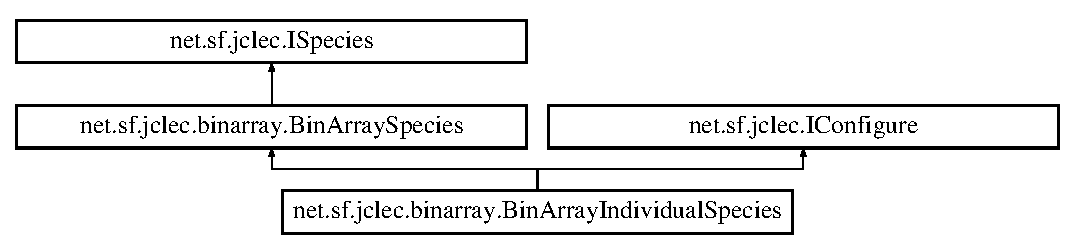
\includegraphics[height=3.888889cm]{classnet_1_1sf_1_1jclec_1_1binarray_1_1_bin_array_individual_species}
\end{center}
\end{figure}
\subsection*{Public Member Functions}
\begin{DoxyCompactItemize}
\item 
\hyperlink{classnet_1_1sf_1_1jclec_1_1binarray_1_1_bin_array_individual_species_adf95507b4f49a30ec6c3be36384f6a32}{Bin\-Array\-Individual\-Species} ()
\item 
\hyperlink{classnet_1_1sf_1_1jclec_1_1binarray_1_1_bin_array_individual_species_ad28b73680937e47b71a9c3b45962f38d}{Bin\-Array\-Individual\-Species} (byte\mbox{[}$\,$\mbox{]} \hyperlink{classnet_1_1sf_1_1jclec_1_1binarray_1_1_bin_array_species_ab0e39779362683e78929877e42c7e660}{genotype\-Schema})
\item 
void \hyperlink{classnet_1_1sf_1_1jclec_1_1binarray_1_1_bin_array_individual_species_a2b57176147a22e2dccefc34bfd958234}{set\-Genotype\-Schema} (byte\mbox{[}$\,$\mbox{]} \hyperlink{classnet_1_1sf_1_1jclec_1_1binarray_1_1_bin_array_species_ab0e39779362683e78929877e42c7e660}{genotype\-Schema})
\item 
\hyperlink{classnet_1_1sf_1_1jclec_1_1binarray_1_1_bin_array_individual}{Bin\-Array\-Individual} \hyperlink{classnet_1_1sf_1_1jclec_1_1binarray_1_1_bin_array_individual_species_a45cde066459dffd8e5ef6584b6d55d15}{create\-Individual} (byte\mbox{[}$\,$\mbox{]} genotype)
\item 
void \hyperlink{classnet_1_1sf_1_1jclec_1_1binarray_1_1_bin_array_individual_species_a11ed22273940f1c00b594f155d95e67c}{configure} (Configuration configuration)
\item 
boolean \hyperlink{classnet_1_1sf_1_1jclec_1_1binarray_1_1_bin_array_individual_species_a5038f5bb6531316528ae9be5e078247a}{equals} (Object other)
\end{DoxyCompactItemize}
\subsection*{Additional Inherited Members}


\subsection{Detailed Description}
\hyperlink{classnet_1_1sf_1_1jclec_1_1binarray_1_1_bin_array_individual}{Bin\-Array\-Individual} species.

Species for individuals of type \char`\"{}\-Bin\-Array\-Individual\char`\"{}. This species set its schema explicitly (using the set\-Schema() method).

\begin{DoxyAuthor}{Author}
Sebastian Ventura 
\end{DoxyAuthor}


\subsection{Constructor \& Destructor Documentation}
\hypertarget{classnet_1_1sf_1_1jclec_1_1binarray_1_1_bin_array_individual_species_adf95507b4f49a30ec6c3be36384f6a32}{\index{net\-::sf\-::jclec\-::binarray\-::\-Bin\-Array\-Individual\-Species@{net\-::sf\-::jclec\-::binarray\-::\-Bin\-Array\-Individual\-Species}!Bin\-Array\-Individual\-Species@{Bin\-Array\-Individual\-Species}}
\index{Bin\-Array\-Individual\-Species@{Bin\-Array\-Individual\-Species}!net::sf::jclec::binarray::BinArrayIndividualSpecies@{net\-::sf\-::jclec\-::binarray\-::\-Bin\-Array\-Individual\-Species}}
\subsubsection[{Bin\-Array\-Individual\-Species}]{\setlength{\rightskip}{0pt plus 5cm}net.\-sf.\-jclec.\-binarray.\-Bin\-Array\-Individual\-Species.\-Bin\-Array\-Individual\-Species (
\begin{DoxyParamCaption}
{}
\end{DoxyParamCaption}
)}}\label{classnet_1_1sf_1_1jclec_1_1binarray_1_1_bin_array_individual_species_adf95507b4f49a30ec6c3be36384f6a32}
Empty constructor \hypertarget{classnet_1_1sf_1_1jclec_1_1binarray_1_1_bin_array_individual_species_ad28b73680937e47b71a9c3b45962f38d}{\index{net\-::sf\-::jclec\-::binarray\-::\-Bin\-Array\-Individual\-Species@{net\-::sf\-::jclec\-::binarray\-::\-Bin\-Array\-Individual\-Species}!Bin\-Array\-Individual\-Species@{Bin\-Array\-Individual\-Species}}
\index{Bin\-Array\-Individual\-Species@{Bin\-Array\-Individual\-Species}!net::sf::jclec::binarray::BinArrayIndividualSpecies@{net\-::sf\-::jclec\-::binarray\-::\-Bin\-Array\-Individual\-Species}}
\subsubsection[{Bin\-Array\-Individual\-Species}]{\setlength{\rightskip}{0pt plus 5cm}net.\-sf.\-jclec.\-binarray.\-Bin\-Array\-Individual\-Species.\-Bin\-Array\-Individual\-Species (
\begin{DoxyParamCaption}
\item[{byte\mbox{[}$\,$\mbox{]}}]{genotype\-Schema}
\end{DoxyParamCaption}
)}}\label{classnet_1_1sf_1_1jclec_1_1binarray_1_1_bin_array_individual_species_ad28b73680937e47b71a9c3b45962f38d}
Constructor that sets individual species 

\subsection{Member Function Documentation}
\hypertarget{classnet_1_1sf_1_1jclec_1_1binarray_1_1_bin_array_individual_species_a11ed22273940f1c00b594f155d95e67c}{\index{net\-::sf\-::jclec\-::binarray\-::\-Bin\-Array\-Individual\-Species@{net\-::sf\-::jclec\-::binarray\-::\-Bin\-Array\-Individual\-Species}!configure@{configure}}
\index{configure@{configure}!net::sf::jclec::binarray::BinArrayIndividualSpecies@{net\-::sf\-::jclec\-::binarray\-::\-Bin\-Array\-Individual\-Species}}
\subsubsection[{configure}]{\setlength{\rightskip}{0pt plus 5cm}void net.\-sf.\-jclec.\-binarray.\-Bin\-Array\-Individual\-Species.\-configure (
\begin{DoxyParamCaption}
\item[{Configuration}]{configuration}
\end{DoxyParamCaption}
)}}\label{classnet_1_1sf_1_1jclec_1_1binarray_1_1_bin_array_individual_species_a11ed22273940f1c00b594f155d95e67c}
Configuration parameters for this species are\-:


\begin{DoxyItemize}
\item {\ttfamily \mbox{[}-\/length\mbox{]} (int)}

Genotype length. If this parameter is set, 'genotype-\/schema' parameter is ignored and all schema positions are set to '$\ast$'.  
\item {\ttfamily genotype-\/schema (String)}

Genotype schema. This parameter contains characters '1', '0' and '$\ast$' to represent schema elements...  
\end{DoxyItemize}

Implements \hyperlink{interfacenet_1_1sf_1_1jclec_1_1_i_configure_add31a65a04d148c690a956fbbad6987c}{net.\-sf.\-jclec.\-I\-Configure}.

\hypertarget{classnet_1_1sf_1_1jclec_1_1binarray_1_1_bin_array_individual_species_a45cde066459dffd8e5ef6584b6d55d15}{\index{net\-::sf\-::jclec\-::binarray\-::\-Bin\-Array\-Individual\-Species@{net\-::sf\-::jclec\-::binarray\-::\-Bin\-Array\-Individual\-Species}!create\-Individual@{create\-Individual}}
\index{create\-Individual@{create\-Individual}!net::sf::jclec::binarray::BinArrayIndividualSpecies@{net\-::sf\-::jclec\-::binarray\-::\-Bin\-Array\-Individual\-Species}}
\subsubsection[{create\-Individual}]{\setlength{\rightskip}{0pt plus 5cm}{\bf Bin\-Array\-Individual} net.\-sf.\-jclec.\-binarray.\-Bin\-Array\-Individual\-Species.\-create\-Individual (
\begin{DoxyParamCaption}
\item[{byte\mbox{[}$\,$\mbox{]}}]{genotype}
\end{DoxyParamCaption}
)\hspace{0.3cm}{\ttfamily [virtual]}}}\label{classnet_1_1sf_1_1jclec_1_1binarray_1_1_bin_array_individual_species_a45cde066459dffd8e5ef6584b6d55d15}
Factory method.


\begin{DoxyParams}{Parameters}
{\em genotype} & Individual genotype \\
\hline
\end{DoxyParams}


Implements \hyperlink{classnet_1_1sf_1_1jclec_1_1binarray_1_1_bin_array_species_a56e839a1fa64ffd8f6a595a63fa8ab28}{net.\-sf.\-jclec.\-binarray.\-Bin\-Array\-Species}.

\hypertarget{classnet_1_1sf_1_1jclec_1_1binarray_1_1_bin_array_individual_species_a5038f5bb6531316528ae9be5e078247a}{\index{net\-::sf\-::jclec\-::binarray\-::\-Bin\-Array\-Individual\-Species@{net\-::sf\-::jclec\-::binarray\-::\-Bin\-Array\-Individual\-Species}!equals@{equals}}
\index{equals@{equals}!net::sf::jclec::binarray::BinArrayIndividualSpecies@{net\-::sf\-::jclec\-::binarray\-::\-Bin\-Array\-Individual\-Species}}
\subsubsection[{equals}]{\setlength{\rightskip}{0pt plus 5cm}boolean net.\-sf.\-jclec.\-binarray.\-Bin\-Array\-Individual\-Species.\-equals (
\begin{DoxyParamCaption}
\item[{Object}]{other}
\end{DoxyParamCaption}
)}}\label{classnet_1_1sf_1_1jclec_1_1binarray_1_1_bin_array_individual_species_a5038f5bb6531316528ae9be5e078247a}
\hypertarget{classnet_1_1sf_1_1jclec_1_1binarray_1_1_bin_array_individual_species_a2b57176147a22e2dccefc34bfd958234}{\index{net\-::sf\-::jclec\-::binarray\-::\-Bin\-Array\-Individual\-Species@{net\-::sf\-::jclec\-::binarray\-::\-Bin\-Array\-Individual\-Species}!set\-Genotype\-Schema@{set\-Genotype\-Schema}}
\index{set\-Genotype\-Schema@{set\-Genotype\-Schema}!net::sf::jclec::binarray::BinArrayIndividualSpecies@{net\-::sf\-::jclec\-::binarray\-::\-Bin\-Array\-Individual\-Species}}
\subsubsection[{set\-Genotype\-Schema}]{\setlength{\rightskip}{0pt plus 5cm}void net.\-sf.\-jclec.\-binarray.\-Bin\-Array\-Individual\-Species.\-set\-Genotype\-Schema (
\begin{DoxyParamCaption}
\item[{byte\mbox{[}$\,$\mbox{]}}]{genotype\-Schema}
\end{DoxyParamCaption}
)}}\label{classnet_1_1sf_1_1jclec_1_1binarray_1_1_bin_array_individual_species_a2b57176147a22e2dccefc34bfd958234}
Sets genotype schema.

This method is used in marshall/unmarshall and configuration methods.


\begin{DoxyParams}{Parameters}
{\em genotype\-Schema} & New genotype schema. \\
\hline
\end{DoxyParams}


The documentation for this class was generated from the following file\-:\begin{DoxyCompactItemize}
\item 
src/main/java/net/sf/jclec/binarray/Bin\-Array\-Individual\-Species.\-java\end{DoxyCompactItemize}

\hypertarget{classnet_1_1sf_1_1jclec_1_1binarray_1_1_bin_array_individual_species_test}{\section{net.\-sf.\-jclec.\-binarray.\-Bin\-Array\-Individual\-Species\-Test Class Reference}
\label{classnet_1_1sf_1_1jclec_1_1binarray_1_1_bin_array_individual_species_test}\index{net.\-sf.\-jclec.\-binarray.\-Bin\-Array\-Individual\-Species\-Test@{net.\-sf.\-jclec.\-binarray.\-Bin\-Array\-Individual\-Species\-Test}}
}


Inherits I\-Configure\-Test$<$ Bin\-Array\-Individual\-Species $>$.



\subsection{Detailed Description}
Marshall and unmarshal tests for \hyperlink{classnet_1_1sf_1_1jclec_1_1binarray_1_1_bin_array_individual_species}{Bin\-Array\-Individual\-Species} class.

\begin{DoxyAuthor}{Author}
Sebastian Ventura 
\end{DoxyAuthor}


The documentation for this class was generated from the following file\-:\begin{DoxyCompactItemize}
\item 
src/test/java/net/sf/jclec/binarray/Bin\-Array\-Individual\-Species\-Test.\-java\end{DoxyCompactItemize}

\hypertarget{classnet_1_1sf_1_1jclec_1_1binarray_1_1_bin_array_mutator}{\section{net.\-sf.\-jclec.\-binarray.\-Bin\-Array\-Mutator Class Reference}
\label{classnet_1_1sf_1_1jclec_1_1binarray_1_1_bin_array_mutator}\index{net.\-sf.\-jclec.\-binarray.\-Bin\-Array\-Mutator@{net.\-sf.\-jclec.\-binarray.\-Bin\-Array\-Mutator}}
}
Inheritance diagram for net.\-sf.\-jclec.\-binarray.\-Bin\-Array\-Mutator\-:\begin{figure}[H]
\begin{center}
\leavevmode
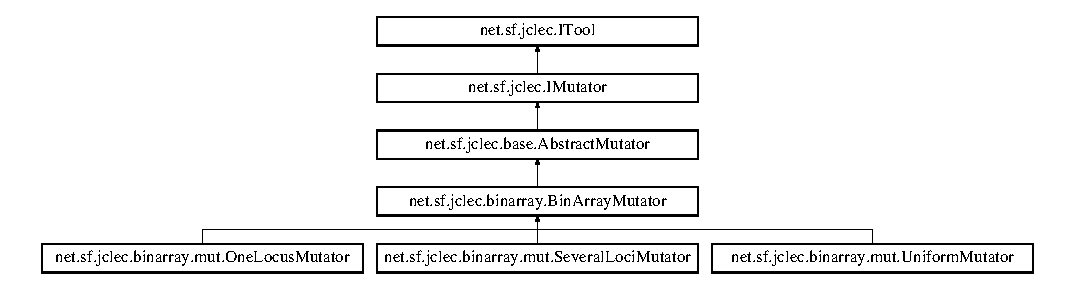
\includegraphics[height=3.431373cm]{classnet_1_1sf_1_1jclec_1_1binarray_1_1_bin_array_mutator}
\end{center}
\end{figure}
\subsection*{Public Member Functions}
\begin{DoxyCompactItemize}
\item 
\hyperlink{classnet_1_1sf_1_1jclec_1_1binarray_1_1_bin_array_mutator_afe2bc031aba996621cce38c7fbb78675}{Bin\-Array\-Mutator} ()
\end{DoxyCompactItemize}
\subsection*{Protected Member Functions}
\begin{DoxyCompactItemize}
\item 
void \hyperlink{classnet_1_1sf_1_1jclec_1_1binarray_1_1_bin_array_mutator_a104587c4458bc8c299cdf902e0ee0cc9}{prepare\-Mutation} ()
\item 
final int \hyperlink{classnet_1_1sf_1_1jclec_1_1binarray_1_1_bin_array_mutator_a6feab6c84b950942298a58b3c5d21fd5}{get\-Mutable\-Locus} ()
\item 
final void \hyperlink{classnet_1_1sf_1_1jclec_1_1binarray_1_1_bin_array_mutator_a6f162a319387eb82bfdb32ff8549ac2f}{flip} (byte\mbox{[}$\,$\mbox{]} chrom, int locus)
\end{DoxyCompactItemize}
\subsection*{Protected Attributes}
\begin{DoxyCompactItemize}
\item 
transient \hyperlink{classnet_1_1sf_1_1jclec_1_1binarray_1_1_bin_array_species}{Bin\-Array\-Species} \hyperlink{classnet_1_1sf_1_1jclec_1_1binarray_1_1_bin_array_mutator_af33a9ab3e0c7729ef86f918c34348080}{species}
\item 
transient byte\mbox{[}$\,$\mbox{]} \hyperlink{classnet_1_1sf_1_1jclec_1_1binarray_1_1_bin_array_mutator_ab89c4bc4bb927685dfb89606bd949808}{schema}
\end{DoxyCompactItemize}


\subsection{Detailed Description}
\hyperlink{classnet_1_1sf_1_1jclec_1_1binarray_1_1_bin_array_individual}{Bin\-Array\-Individual} (and subclasses) specific mutator.

\begin{DoxyAuthor}{Author}
Sebastian Ventura 
\end{DoxyAuthor}


\subsection{Constructor \& Destructor Documentation}
\hypertarget{classnet_1_1sf_1_1jclec_1_1binarray_1_1_bin_array_mutator_afe2bc031aba996621cce38c7fbb78675}{\index{net\-::sf\-::jclec\-::binarray\-::\-Bin\-Array\-Mutator@{net\-::sf\-::jclec\-::binarray\-::\-Bin\-Array\-Mutator}!Bin\-Array\-Mutator@{Bin\-Array\-Mutator}}
\index{Bin\-Array\-Mutator@{Bin\-Array\-Mutator}!net::sf::jclec::binarray::BinArrayMutator@{net\-::sf\-::jclec\-::binarray\-::\-Bin\-Array\-Mutator}}
\subsubsection[{Bin\-Array\-Mutator}]{\setlength{\rightskip}{0pt plus 5cm}net.\-sf.\-jclec.\-binarray.\-Bin\-Array\-Mutator.\-Bin\-Array\-Mutator (
\begin{DoxyParamCaption}
{}
\end{DoxyParamCaption}
)}}\label{classnet_1_1sf_1_1jclec_1_1binarray_1_1_bin_array_mutator_afe2bc031aba996621cce38c7fbb78675}
Empty (default) constructor. 

\subsection{Member Function Documentation}
\hypertarget{classnet_1_1sf_1_1jclec_1_1binarray_1_1_bin_array_mutator_a6f162a319387eb82bfdb32ff8549ac2f}{\index{net\-::sf\-::jclec\-::binarray\-::\-Bin\-Array\-Mutator@{net\-::sf\-::jclec\-::binarray\-::\-Bin\-Array\-Mutator}!flip@{flip}}
\index{flip@{flip}!net::sf::jclec::binarray::BinArrayMutator@{net\-::sf\-::jclec\-::binarray\-::\-Bin\-Array\-Mutator}}
\subsubsection[{flip}]{\setlength{\rightskip}{0pt plus 5cm}final void net.\-sf.\-jclec.\-binarray.\-Bin\-Array\-Mutator.\-flip (
\begin{DoxyParamCaption}
\item[{byte\mbox{[}$\,$\mbox{]}}]{chrom, }
\item[{int}]{locus}
\end{DoxyParamCaption}
)\hspace{0.3cm}{\ttfamily [protected]}}}\label{classnet_1_1sf_1_1jclec_1_1binarray_1_1_bin_array_mutator_a6f162a319387eb82bfdb32ff8549ac2f}
Flip method.


\begin{DoxyParams}{Parameters}
{\em chrom} & Chromosome affected \\
\hline
{\em locus} & Locus affected \\
\hline
\end{DoxyParams}
\hypertarget{classnet_1_1sf_1_1jclec_1_1binarray_1_1_bin_array_mutator_a6feab6c84b950942298a58b3c5d21fd5}{\index{net\-::sf\-::jclec\-::binarray\-::\-Bin\-Array\-Mutator@{net\-::sf\-::jclec\-::binarray\-::\-Bin\-Array\-Mutator}!get\-Mutable\-Locus@{get\-Mutable\-Locus}}
\index{get\-Mutable\-Locus@{get\-Mutable\-Locus}!net::sf::jclec::binarray::BinArrayMutator@{net\-::sf\-::jclec\-::binarray\-::\-Bin\-Array\-Mutator}}
\subsubsection[{get\-Mutable\-Locus}]{\setlength{\rightskip}{0pt plus 5cm}final int net.\-sf.\-jclec.\-binarray.\-Bin\-Array\-Mutator.\-get\-Mutable\-Locus (
\begin{DoxyParamCaption}
{}
\end{DoxyParamCaption}
)\hspace{0.3cm}{\ttfamily [protected]}}}\label{classnet_1_1sf_1_1jclec_1_1binarray_1_1_bin_array_mutator_a6feab6c84b950942298a58b3c5d21fd5}
Gets a mutate locus in represented individuals \hypertarget{classnet_1_1sf_1_1jclec_1_1binarray_1_1_bin_array_mutator_a104587c4458bc8c299cdf902e0ee0cc9}{\index{net\-::sf\-::jclec\-::binarray\-::\-Bin\-Array\-Mutator@{net\-::sf\-::jclec\-::binarray\-::\-Bin\-Array\-Mutator}!prepare\-Mutation@{prepare\-Mutation}}
\index{prepare\-Mutation@{prepare\-Mutation}!net::sf::jclec::binarray::BinArrayMutator@{net\-::sf\-::jclec\-::binarray\-::\-Bin\-Array\-Mutator}}
\subsubsection[{prepare\-Mutation}]{\setlength{\rightskip}{0pt plus 5cm}void net.\-sf.\-jclec.\-binarray.\-Bin\-Array\-Mutator.\-prepare\-Mutation (
\begin{DoxyParamCaption}
{}
\end{DoxyParamCaption}
)\hspace{0.3cm}{\ttfamily [protected]}, {\ttfamily [virtual]}}}\label{classnet_1_1sf_1_1jclec_1_1binarray_1_1_bin_array_mutator_a104587c4458bc8c299cdf902e0ee0cc9}
Prepare mutation process. 

Implements \hyperlink{classnet_1_1sf_1_1jclec_1_1base_1_1_abstract_mutator_ad12e6a2be8fb6082255ce8f399c9b166}{net.\-sf.\-jclec.\-base.\-Abstract\-Mutator}.



\subsection{Member Data Documentation}
\hypertarget{classnet_1_1sf_1_1jclec_1_1binarray_1_1_bin_array_mutator_ab89c4bc4bb927685dfb89606bd949808}{\index{net\-::sf\-::jclec\-::binarray\-::\-Bin\-Array\-Mutator@{net\-::sf\-::jclec\-::binarray\-::\-Bin\-Array\-Mutator}!schema@{schema}}
\index{schema@{schema}!net::sf::jclec::binarray::BinArrayMutator@{net\-::sf\-::jclec\-::binarray\-::\-Bin\-Array\-Mutator}}
\subsubsection[{schema}]{\setlength{\rightskip}{0pt plus 5cm}transient byte \mbox{[}$\,$\mbox{]} net.\-sf.\-jclec.\-binarray.\-Bin\-Array\-Mutator.\-schema\hspace{0.3cm}{\ttfamily [protected]}}}\label{classnet_1_1sf_1_1jclec_1_1binarray_1_1_bin_array_mutator_ab89c4bc4bb927685dfb89606bd949808}
Genotype schema \hypertarget{classnet_1_1sf_1_1jclec_1_1binarray_1_1_bin_array_mutator_af33a9ab3e0c7729ef86f918c34348080}{\index{net\-::sf\-::jclec\-::binarray\-::\-Bin\-Array\-Mutator@{net\-::sf\-::jclec\-::binarray\-::\-Bin\-Array\-Mutator}!species@{species}}
\index{species@{species}!net::sf::jclec::binarray::BinArrayMutator@{net\-::sf\-::jclec\-::binarray\-::\-Bin\-Array\-Mutator}}
\subsubsection[{species}]{\setlength{\rightskip}{0pt plus 5cm}transient {\bf Bin\-Array\-Species} net.\-sf.\-jclec.\-binarray.\-Bin\-Array\-Mutator.\-species\hspace{0.3cm}{\ttfamily [protected]}}}\label{classnet_1_1sf_1_1jclec_1_1binarray_1_1_bin_array_mutator_af33a9ab3e0c7729ef86f918c34348080}
Individual species (taked from execution context) 

The documentation for this class was generated from the following file\-:\begin{DoxyCompactItemize}
\item 
src/main/java/net/sf/jclec/binarray/Bin\-Array\-Mutator.\-java\end{DoxyCompactItemize}

\hypertarget{classnet_1_1sf_1_1jclec_1_1binarray_1_1_bin_array_mutator_test_3_01_m_01extends_01_bin_array_mutator_01_4}{\section{net.\-sf.\-jclec.\-binarray.\-Bin\-Array\-Mutator\-Test$<$ M extends Bin\-Array\-Mutator $>$ Class Reference}
\label{classnet_1_1sf_1_1jclec_1_1binarray_1_1_bin_array_mutator_test_3_01_m_01extends_01_bin_array_mutator_01_4}\index{net.\-sf.\-jclec.\-binarray.\-Bin\-Array\-Mutator\-Test$<$ M extends Bin\-Array\-Mutator $>$@{net.\-sf.\-jclec.\-binarray.\-Bin\-Array\-Mutator\-Test$<$ M extends Bin\-Array\-Mutator $>$}}
}


Inherits I\-Mutator\-Test$<$ M $>$.

\subsection*{Protected Member Functions}
\begin{DoxyCompactItemize}
\item 
void \hyperlink{classnet_1_1sf_1_1jclec_1_1binarray_1_1_bin_array_mutator_test_3_01_m_01extends_01_bin_array_mutator_01_4_a3e0bd4e6510091465a54cd9b972de180}{create\-Parents} ()
\end{DoxyCompactItemize}


\subsection{Detailed Description}
Unitary test for class that extends \hyperlink{classnet_1_1sf_1_1jclec_1_1binarray_1_1_bin_array_mutator}{Bin\-Array\-Mutator}.

\begin{DoxyAuthor}{Author}
Sebastian Ventura
\end{DoxyAuthor}

\begin{DoxyParams}{Parameters}
{\em $<$\-M$>$} & Type of Mutator \\
\hline
\end{DoxyParams}


\subsection{Member Function Documentation}
\hypertarget{classnet_1_1sf_1_1jclec_1_1binarray_1_1_bin_array_mutator_test_3_01_m_01extends_01_bin_array_mutator_01_4_a3e0bd4e6510091465a54cd9b972de180}{\index{net\-::sf\-::jclec\-::binarray\-::\-Bin\-Array\-Mutator\-Test$<$ M extends Bin\-Array\-Mutator $>$@{net\-::sf\-::jclec\-::binarray\-::\-Bin\-Array\-Mutator\-Test$<$ M extends Bin\-Array\-Mutator $>$}!create\-Parents@{create\-Parents}}
\index{create\-Parents@{create\-Parents}!net::sf::jclec::binarray::BinArrayMutatorTest< M extends BinArrayMutator >@{net\-::sf\-::jclec\-::binarray\-::\-Bin\-Array\-Mutator\-Test$<$ M extends Bin\-Array\-Mutator $>$}}
\subsubsection[{create\-Parents}]{\setlength{\rightskip}{0pt plus 5cm}void net.\-sf.\-jclec.\-binarray.\-Bin\-Array\-Mutator\-Test$<$ M extends {\bf Bin\-Array\-Mutator} $>$.create\-Parents (
\begin{DoxyParamCaption}
{}
\end{DoxyParamCaption}
)\hspace{0.3cm}{\ttfamily [protected]}}}\label{classnet_1_1sf_1_1jclec_1_1binarray_1_1_bin_array_mutator_test_3_01_m_01extends_01_bin_array_mutator_01_4_a3e0bd4e6510091465a54cd9b972de180}
Mutant is (1,1,1,1,1,1)

The documentation for this class was generated from the following file\-:\begin{DoxyCompactItemize}
\item 
src/test/java/net/sf/jclec/binarray/Bin\-Array\-Mutator\-Test.\-java\end{DoxyCompactItemize}

\hypertarget{classnet_1_1sf_1_1jclec_1_1binarray_1_1_bin_array_recombinator}{\section{net.\-sf.\-jclec.\-binarray.\-Bin\-Array\-Recombinator Class Reference}
\label{classnet_1_1sf_1_1jclec_1_1binarray_1_1_bin_array_recombinator}\index{net.\-sf.\-jclec.\-binarray.\-Bin\-Array\-Recombinator@{net.\-sf.\-jclec.\-binarray.\-Bin\-Array\-Recombinator}}
}
Inheritance diagram for net.\-sf.\-jclec.\-binarray.\-Bin\-Array\-Recombinator\-:\begin{figure}[H]
\begin{center}
\leavevmode
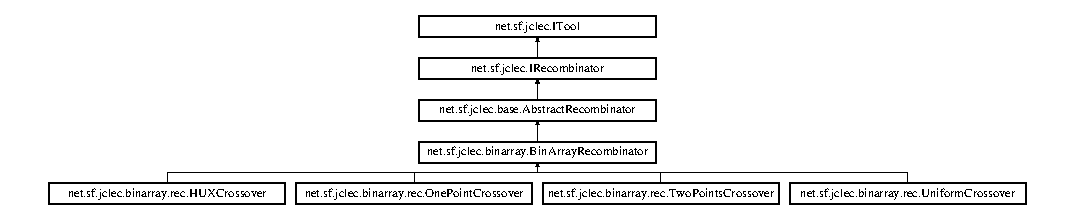
\includegraphics[height=2.527076cm]{classnet_1_1sf_1_1jclec_1_1binarray_1_1_bin_array_recombinator}
\end{center}
\end{figure}
\subsection*{Public Member Functions}
\begin{DoxyCompactItemize}
\item 
\hyperlink{classnet_1_1sf_1_1jclec_1_1binarray_1_1_bin_array_recombinator_a1234e043f0be3214049bef69e08678ea}{Bin\-Array\-Recombinator} ()
\end{DoxyCompactItemize}
\subsection*{Protected Member Functions}
\begin{DoxyCompactItemize}
\item 
void \hyperlink{classnet_1_1sf_1_1jclec_1_1binarray_1_1_bin_array_recombinator_a8ecb2813d8dca18e20c7673d94efc315}{set\-Ppl} ()
\item 
void \hyperlink{classnet_1_1sf_1_1jclec_1_1binarray_1_1_bin_array_recombinator_a39e8897cd7cd2e4f8ba312432405c7c7}{set\-Spl} ()
\item 
void \hyperlink{classnet_1_1sf_1_1jclec_1_1binarray_1_1_bin_array_recombinator_adfb02ddf2e1aa3a0f3d59229f3b4334b}{prepare\-Recombination} ()
\end{DoxyCompactItemize}
\subsection*{Protected Attributes}
\begin{DoxyCompactItemize}
\item 
transient \hyperlink{classnet_1_1sf_1_1jclec_1_1binarray_1_1_bin_array_species}{Bin\-Array\-Species} \hyperlink{classnet_1_1sf_1_1jclec_1_1binarray_1_1_bin_array_recombinator_a2c6a3f232ba4e07edab964e66459d6bb}{species}
\end{DoxyCompactItemize}


\subsection{Detailed Description}
\hyperlink{classnet_1_1sf_1_1jclec_1_1binarray_1_1_bin_array_individual}{Bin\-Array\-Individual} (and subclasses) specific recombinator.

\begin{DoxyAuthor}{Author}
Sebastian Ventura 
\end{DoxyAuthor}


\subsection{Constructor \& Destructor Documentation}
\hypertarget{classnet_1_1sf_1_1jclec_1_1binarray_1_1_bin_array_recombinator_a1234e043f0be3214049bef69e08678ea}{\index{net\-::sf\-::jclec\-::binarray\-::\-Bin\-Array\-Recombinator@{net\-::sf\-::jclec\-::binarray\-::\-Bin\-Array\-Recombinator}!Bin\-Array\-Recombinator@{Bin\-Array\-Recombinator}}
\index{Bin\-Array\-Recombinator@{Bin\-Array\-Recombinator}!net::sf::jclec::binarray::BinArrayRecombinator@{net\-::sf\-::jclec\-::binarray\-::\-Bin\-Array\-Recombinator}}
\subsubsection[{Bin\-Array\-Recombinator}]{\setlength{\rightskip}{0pt plus 5cm}net.\-sf.\-jclec.\-binarray.\-Bin\-Array\-Recombinator.\-Bin\-Array\-Recombinator (
\begin{DoxyParamCaption}
{}
\end{DoxyParamCaption}
)}}\label{classnet_1_1sf_1_1jclec_1_1binarray_1_1_bin_array_recombinator_a1234e043f0be3214049bef69e08678ea}
Empty (default) constructor. 

\subsection{Member Function Documentation}
\hypertarget{classnet_1_1sf_1_1jclec_1_1binarray_1_1_bin_array_recombinator_adfb02ddf2e1aa3a0f3d59229f3b4334b}{\index{net\-::sf\-::jclec\-::binarray\-::\-Bin\-Array\-Recombinator@{net\-::sf\-::jclec\-::binarray\-::\-Bin\-Array\-Recombinator}!prepare\-Recombination@{prepare\-Recombination}}
\index{prepare\-Recombination@{prepare\-Recombination}!net::sf::jclec::binarray::BinArrayRecombinator@{net\-::sf\-::jclec\-::binarray\-::\-Bin\-Array\-Recombinator}}
\subsubsection[{prepare\-Recombination}]{\setlength{\rightskip}{0pt plus 5cm}void net.\-sf.\-jclec.\-binarray.\-Bin\-Array\-Recombinator.\-prepare\-Recombination (
\begin{DoxyParamCaption}
{}
\end{DoxyParamCaption}
)\hspace{0.3cm}{\ttfamily [protected]}, {\ttfamily [virtual]}}}\label{classnet_1_1sf_1_1jclec_1_1binarray_1_1_bin_array_recombinator_adfb02ddf2e1aa3a0f3d59229f3b4334b}
Prepare recombination process. 

Implements \hyperlink{classnet_1_1sf_1_1jclec_1_1base_1_1_abstract_recombinator_ad9518cc41f28166465c4b8dc60059048}{net.\-sf.\-jclec.\-base.\-Abstract\-Recombinator}.

\hypertarget{classnet_1_1sf_1_1jclec_1_1binarray_1_1_bin_array_recombinator_a8ecb2813d8dca18e20c7673d94efc315}{\index{net\-::sf\-::jclec\-::binarray\-::\-Bin\-Array\-Recombinator@{net\-::sf\-::jclec\-::binarray\-::\-Bin\-Array\-Recombinator}!set\-Ppl@{set\-Ppl}}
\index{set\-Ppl@{set\-Ppl}!net::sf::jclec::binarray::BinArrayRecombinator@{net\-::sf\-::jclec\-::binarray\-::\-Bin\-Array\-Recombinator}}
\subsubsection[{set\-Ppl}]{\setlength{\rightskip}{0pt plus 5cm}void net.\-sf.\-jclec.\-binarray.\-Bin\-Array\-Recombinator.\-set\-Ppl (
\begin{DoxyParamCaption}
{}
\end{DoxyParamCaption}
)\hspace{0.3cm}{\ttfamily [protected]}, {\ttfamily [virtual]}}}\label{classnet_1_1sf_1_1jclec_1_1binarray_1_1_bin_array_recombinator_a8ecb2813d8dca18e20c7673d94efc315}
Set ppl=2 

Implements \hyperlink{classnet_1_1sf_1_1jclec_1_1base_1_1_abstract_recombinator_aa90f858c27f9da69b2f7bb0a9220ed4e}{net.\-sf.\-jclec.\-base.\-Abstract\-Recombinator}.

\hypertarget{classnet_1_1sf_1_1jclec_1_1binarray_1_1_bin_array_recombinator_a39e8897cd7cd2e4f8ba312432405c7c7}{\index{net\-::sf\-::jclec\-::binarray\-::\-Bin\-Array\-Recombinator@{net\-::sf\-::jclec\-::binarray\-::\-Bin\-Array\-Recombinator}!set\-Spl@{set\-Spl}}
\index{set\-Spl@{set\-Spl}!net::sf::jclec::binarray::BinArrayRecombinator@{net\-::sf\-::jclec\-::binarray\-::\-Bin\-Array\-Recombinator}}
\subsubsection[{set\-Spl}]{\setlength{\rightskip}{0pt plus 5cm}void net.\-sf.\-jclec.\-binarray.\-Bin\-Array\-Recombinator.\-set\-Spl (
\begin{DoxyParamCaption}
{}
\end{DoxyParamCaption}
)\hspace{0.3cm}{\ttfamily [protected]}, {\ttfamily [virtual]}}}\label{classnet_1_1sf_1_1jclec_1_1binarray_1_1_bin_array_recombinator_a39e8897cd7cd2e4f8ba312432405c7c7}
Set spl=2 

Implements \hyperlink{classnet_1_1sf_1_1jclec_1_1base_1_1_abstract_recombinator_a49a445f27d777d6f439d97d61f2e1729}{net.\-sf.\-jclec.\-base.\-Abstract\-Recombinator}.



\subsection{Member Data Documentation}
\hypertarget{classnet_1_1sf_1_1jclec_1_1binarray_1_1_bin_array_recombinator_a2c6a3f232ba4e07edab964e66459d6bb}{\index{net\-::sf\-::jclec\-::binarray\-::\-Bin\-Array\-Recombinator@{net\-::sf\-::jclec\-::binarray\-::\-Bin\-Array\-Recombinator}!species@{species}}
\index{species@{species}!net::sf::jclec::binarray::BinArrayRecombinator@{net\-::sf\-::jclec\-::binarray\-::\-Bin\-Array\-Recombinator}}
\subsubsection[{species}]{\setlength{\rightskip}{0pt plus 5cm}transient {\bf Bin\-Array\-Species} net.\-sf.\-jclec.\-binarray.\-Bin\-Array\-Recombinator.\-species\hspace{0.3cm}{\ttfamily [protected]}}}\label{classnet_1_1sf_1_1jclec_1_1binarray_1_1_bin_array_recombinator_a2c6a3f232ba4e07edab964e66459d6bb}
Individual species (taked from execution context) 

The documentation for this class was generated from the following file\-:\begin{DoxyCompactItemize}
\item 
src/main/java/net/sf/jclec/binarray/Bin\-Array\-Recombinator.\-java\end{DoxyCompactItemize}

\hypertarget{classnet_1_1sf_1_1jclec_1_1binarray_1_1_bin_array_species}{\section{net.\-sf.\-jclec.\-binarray.\-Bin\-Array\-Species Class Reference}
\label{classnet_1_1sf_1_1jclec_1_1binarray_1_1_bin_array_species}\index{net.\-sf.\-jclec.\-binarray.\-Bin\-Array\-Species@{net.\-sf.\-jclec.\-binarray.\-Bin\-Array\-Species}}
}
Inheritance diagram for net.\-sf.\-jclec.\-binarray.\-Bin\-Array\-Species\-:\begin{figure}[H]
\begin{center}
\leavevmode
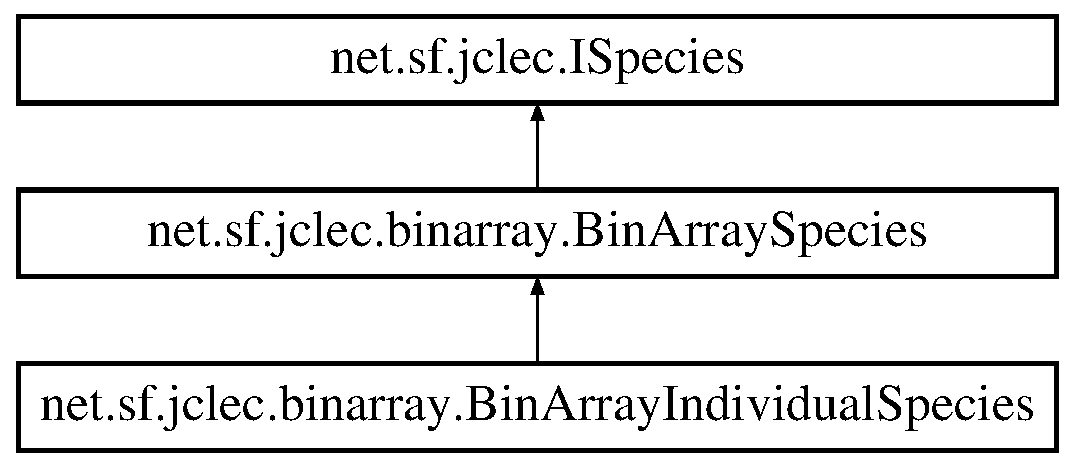
\includegraphics[height=3.000000cm]{classnet_1_1sf_1_1jclec_1_1binarray_1_1_bin_array_species}
\end{center}
\end{figure}
\subsection*{Public Member Functions}
\begin{DoxyCompactItemize}
\item 
\hyperlink{classnet_1_1sf_1_1jclec_1_1binarray_1_1_bin_array_species_ab19cefea88f3534de20bdfdf86fc7e49}{Bin\-Array\-Species} ()
\item 
abstract \hyperlink{classnet_1_1sf_1_1jclec_1_1binarray_1_1_bin_array_individual}{Bin\-Array\-Individual} \hyperlink{classnet_1_1sf_1_1jclec_1_1binarray_1_1_bin_array_species_a56e839a1fa64ffd8f6a595a63fa8ab28}{create\-Individual} (byte\mbox{[}$\,$\mbox{]} genotype)
\item 
int \hyperlink{classnet_1_1sf_1_1jclec_1_1binarray_1_1_bin_array_species_ab7d920897365990a3414db257bdaf743}{get\-Genotype\-Length} ()
\item 
byte\mbox{[}$\,$\mbox{]} \hyperlink{classnet_1_1sf_1_1jclec_1_1binarray_1_1_bin_array_species_a70e09b5cd11270151b6c9b6e02feedf9}{get\-Genotype\-Schema} ()
\end{DoxyCompactItemize}
\subsection*{Protected Attributes}
\begin{DoxyCompactItemize}
\item 
byte\mbox{[}$\,$\mbox{]} \hyperlink{classnet_1_1sf_1_1jclec_1_1binarray_1_1_bin_array_species_ab0e39779362683e78929877e42c7e660}{genotype\-Schema}
\end{DoxyCompactItemize}


\subsection{Detailed Description}
Abstract implementation for I\-Bin\-Array\-Species.

This class contains a byte array that contains the genotype schema for all represented individuals. This schema can be set in a subclass of this or can be calculated from other problem information.

\begin{DoxyAuthor}{Author}
Sebastian Ventura
\end{DoxyAuthor}
\begin{DoxySeeAlso}{See Also}
\hyperlink{classnet_1_1sf_1_1jclec_1_1binarray_1_1_bin_array_individual_species}{Bin\-Array\-Individual\-Species} 
\end{DoxySeeAlso}


\subsection{Constructor \& Destructor Documentation}
\hypertarget{classnet_1_1sf_1_1jclec_1_1binarray_1_1_bin_array_species_ab19cefea88f3534de20bdfdf86fc7e49}{\index{net\-::sf\-::jclec\-::binarray\-::\-Bin\-Array\-Species@{net\-::sf\-::jclec\-::binarray\-::\-Bin\-Array\-Species}!Bin\-Array\-Species@{Bin\-Array\-Species}}
\index{Bin\-Array\-Species@{Bin\-Array\-Species}!net::sf::jclec::binarray::BinArraySpecies@{net\-::sf\-::jclec\-::binarray\-::\-Bin\-Array\-Species}}
\subsubsection[{Bin\-Array\-Species}]{\setlength{\rightskip}{0pt plus 5cm}net.\-sf.\-jclec.\-binarray.\-Bin\-Array\-Species.\-Bin\-Array\-Species (
\begin{DoxyParamCaption}
{}
\end{DoxyParamCaption}
)}}\label{classnet_1_1sf_1_1jclec_1_1binarray_1_1_bin_array_species_ab19cefea88f3534de20bdfdf86fc7e49}
Empty constructor 

\subsection{Member Function Documentation}
\hypertarget{classnet_1_1sf_1_1jclec_1_1binarray_1_1_bin_array_species_a56e839a1fa64ffd8f6a595a63fa8ab28}{\index{net\-::sf\-::jclec\-::binarray\-::\-Bin\-Array\-Species@{net\-::sf\-::jclec\-::binarray\-::\-Bin\-Array\-Species}!create\-Individual@{create\-Individual}}
\index{create\-Individual@{create\-Individual}!net::sf::jclec::binarray::BinArraySpecies@{net\-::sf\-::jclec\-::binarray\-::\-Bin\-Array\-Species}}
\subsubsection[{create\-Individual}]{\setlength{\rightskip}{0pt plus 5cm}abstract {\bf Bin\-Array\-Individual} net.\-sf.\-jclec.\-binarray.\-Bin\-Array\-Species.\-create\-Individual (
\begin{DoxyParamCaption}
\item[{byte\mbox{[}$\,$\mbox{]}}]{genotype}
\end{DoxyParamCaption}
)\hspace{0.3cm}{\ttfamily [pure virtual]}}}\label{classnet_1_1sf_1_1jclec_1_1binarray_1_1_bin_array_species_a56e839a1fa64ffd8f6a595a63fa8ab28}
Factory method.


\begin{DoxyParams}{Parameters}
{\em genotype} & Individual genotype.\\
\hline
\end{DoxyParams}
\begin{DoxyReturn}{Returns}
A new instance of represented class 
\end{DoxyReturn}


Implemented in \hyperlink{classnet_1_1sf_1_1jclec_1_1binarray_1_1_bin_array_individual_species_a45cde066459dffd8e5ef6584b6d55d15}{net.\-sf.\-jclec.\-binarray.\-Bin\-Array\-Individual\-Species}.

\hypertarget{classnet_1_1sf_1_1jclec_1_1binarray_1_1_bin_array_species_ab7d920897365990a3414db257bdaf743}{\index{net\-::sf\-::jclec\-::binarray\-::\-Bin\-Array\-Species@{net\-::sf\-::jclec\-::binarray\-::\-Bin\-Array\-Species}!get\-Genotype\-Length@{get\-Genotype\-Length}}
\index{get\-Genotype\-Length@{get\-Genotype\-Length}!net::sf::jclec::binarray::BinArraySpecies@{net\-::sf\-::jclec\-::binarray\-::\-Bin\-Array\-Species}}
\subsubsection[{get\-Genotype\-Length}]{\setlength{\rightskip}{0pt plus 5cm}int net.\-sf.\-jclec.\-binarray.\-Bin\-Array\-Species.\-get\-Genotype\-Length (
\begin{DoxyParamCaption}
{}
\end{DoxyParamCaption}
)}}\label{classnet_1_1sf_1_1jclec_1_1binarray_1_1_bin_array_species_ab7d920897365990a3414db257bdaf743}
Informs about individual genotype length.

\begin{DoxyReturn}{Returns}
\hyperlink{classnet_1_1sf_1_1jclec_1_1binarray_1_1_bin_array_species_a70e09b5cd11270151b6c9b6e02feedf9}{get\-Genotype\-Schema()}.length 
\end{DoxyReturn}
\hypertarget{classnet_1_1sf_1_1jclec_1_1binarray_1_1_bin_array_species_a70e09b5cd11270151b6c9b6e02feedf9}{\index{net\-::sf\-::jclec\-::binarray\-::\-Bin\-Array\-Species@{net\-::sf\-::jclec\-::binarray\-::\-Bin\-Array\-Species}!get\-Genotype\-Schema@{get\-Genotype\-Schema}}
\index{get\-Genotype\-Schema@{get\-Genotype\-Schema}!net::sf::jclec::binarray::BinArraySpecies@{net\-::sf\-::jclec\-::binarray\-::\-Bin\-Array\-Species}}
\subsubsection[{get\-Genotype\-Schema}]{\setlength{\rightskip}{0pt plus 5cm}byte \mbox{[}$\,$\mbox{]} net.\-sf.\-jclec.\-binarray.\-Bin\-Array\-Species.\-get\-Genotype\-Schema (
\begin{DoxyParamCaption}
{}
\end{DoxyParamCaption}
)}}\label{classnet_1_1sf_1_1jclec_1_1binarray_1_1_bin_array_species_a70e09b5cd11270151b6c9b6e02feedf9}
\begin{DoxyReturn}{Returns}
This genotype schema 
\end{DoxyReturn}


\subsection{Member Data Documentation}
\hypertarget{classnet_1_1sf_1_1jclec_1_1binarray_1_1_bin_array_species_ab0e39779362683e78929877e42c7e660}{\index{net\-::sf\-::jclec\-::binarray\-::\-Bin\-Array\-Species@{net\-::sf\-::jclec\-::binarray\-::\-Bin\-Array\-Species}!genotype\-Schema@{genotype\-Schema}}
\index{genotype\-Schema@{genotype\-Schema}!net::sf::jclec::binarray::BinArraySpecies@{net\-::sf\-::jclec\-::binarray\-::\-Bin\-Array\-Species}}
\subsubsection[{genotype\-Schema}]{\setlength{\rightskip}{0pt plus 5cm}byte \mbox{[}$\,$\mbox{]} net.\-sf.\-jclec.\-binarray.\-Bin\-Array\-Species.\-genotype\-Schema\hspace{0.3cm}{\ttfamily [protected]}}}\label{classnet_1_1sf_1_1jclec_1_1binarray_1_1_bin_array_species_ab0e39779362683e78929877e42c7e660}
Genotype schema 

The documentation for this class was generated from the following file\-:\begin{DoxyCompactItemize}
\item 
src/main/java/net/sf/jclec/binarray/Bin\-Array\-Species.\-java\end{DoxyCompactItemize}

\hypertarget{classnet_1_1sf_1_1jclec_1_1realarray_1_1rec_1_1_b_l_x_alpha_crossover}{\section{net.\-sf.\-jclec.\-realarray.\-rec.\-B\-L\-X\-Alpha\-Crossover Class Reference}
\label{classnet_1_1sf_1_1jclec_1_1realarray_1_1rec_1_1_b_l_x_alpha_crossover}\index{net.\-sf.\-jclec.\-realarray.\-rec.\-B\-L\-X\-Alpha\-Crossover@{net.\-sf.\-jclec.\-realarray.\-rec.\-B\-L\-X\-Alpha\-Crossover}}
}


Inherits net.\-sf.\-jclec.\-realarray.\-rec.\-Uniform\-Crossover2x1.

\subsection*{Public Member Functions}
\begin{DoxyCompactItemize}
\item 
\hyperlink{classnet_1_1sf_1_1jclec_1_1realarray_1_1rec_1_1_b_l_x_alpha_crossover_a3f5cbb9827b1270f217c46e66d950d79}{B\-L\-X\-Alpha\-Crossover} ()
\item 
\hyperlink{classnet_1_1sf_1_1jclec_1_1realarray_1_1rec_1_1_b_l_x_alpha_crossover_aa6a07809ad3114c6d8f8636749e77043}{B\-L\-X\-Alpha\-Crossover} (\hyperlink{interfacenet_1_1sf_1_1jclec_1_1_i_population}{I\-Population} \hyperlink{classnet_1_1sf_1_1jclec_1_1base_1_1_abstract_recombinator_a580de9e9511dbb1d9042eb1089e767a7}{context})
\item 
final double \hyperlink{classnet_1_1sf_1_1jclec_1_1realarray_1_1rec_1_1_b_l_x_alpha_crossover_a389b0a0dd9dd57e396195ccf0ad5326c}{get\-Alpha} ()
\item 
final void \hyperlink{classnet_1_1sf_1_1jclec_1_1realarray_1_1rec_1_1_b_l_x_alpha_crossover_ad95c3d7bb01920d695dfab205eb82d89}{set\-Alpha} (double \hyperlink{classnet_1_1sf_1_1jclec_1_1realarray_1_1rec_1_1_b_l_x_alpha_crossover_a2eae05311a51136efa625d718bcb33b4}{alpha})
\item 
void \hyperlink{classnet_1_1sf_1_1jclec_1_1realarray_1_1rec_1_1_b_l_x_alpha_crossover_a19e22e8da08fe5dc86e6c256dc56fe18}{configure} (Configuration settings)
\end{DoxyCompactItemize}
\subsection*{Protected Member Functions}
\begin{DoxyCompactItemize}
\item 
double \hyperlink{classnet_1_1sf_1_1jclec_1_1realarray_1_1rec_1_1_b_l_x_alpha_crossover_a8d8cd581a6b2ea609c0eb5eb1c580b1a}{default\-Locus\-Rec\-Prob} ()
\end{DoxyCompactItemize}
\subsection*{Protected Attributes}
\begin{DoxyCompactItemize}
\item 
double \hyperlink{classnet_1_1sf_1_1jclec_1_1realarray_1_1rec_1_1_b_l_x_alpha_crossover_a2eae05311a51136efa625d718bcb33b4}{alpha}
\end{DoxyCompactItemize}


\subsection{Detailed Description}
Apply the B\-L\-X-\/alfa crossover for two individuals. This crossover depends on alfa parameter which decides the crossover interval. If alfa value is zero, this crossover is equal than flat crossover.

\begin{DoxyAuthor}{Author}
Alberto Lamarca 

Sebastian Ventura 
\end{DoxyAuthor}


\subsection{Constructor \& Destructor Documentation}
\hypertarget{classnet_1_1sf_1_1jclec_1_1realarray_1_1rec_1_1_b_l_x_alpha_crossover_a3f5cbb9827b1270f217c46e66d950d79}{\index{net\-::sf\-::jclec\-::realarray\-::rec\-::\-B\-L\-X\-Alpha\-Crossover@{net\-::sf\-::jclec\-::realarray\-::rec\-::\-B\-L\-X\-Alpha\-Crossover}!B\-L\-X\-Alpha\-Crossover@{B\-L\-X\-Alpha\-Crossover}}
\index{B\-L\-X\-Alpha\-Crossover@{B\-L\-X\-Alpha\-Crossover}!net::sf::jclec::realarray::rec::BLXAlphaCrossover@{net\-::sf\-::jclec\-::realarray\-::rec\-::\-B\-L\-X\-Alpha\-Crossover}}
\subsubsection[{B\-L\-X\-Alpha\-Crossover}]{\setlength{\rightskip}{0pt plus 5cm}net.\-sf.\-jclec.\-realarray.\-rec.\-B\-L\-X\-Alpha\-Crossover.\-B\-L\-X\-Alpha\-Crossover (
\begin{DoxyParamCaption}
{}
\end{DoxyParamCaption}
)}}\label{classnet_1_1sf_1_1jclec_1_1realarray_1_1rec_1_1_b_l_x_alpha_crossover_a3f5cbb9827b1270f217c46e66d950d79}
Empty constructor \hypertarget{classnet_1_1sf_1_1jclec_1_1realarray_1_1rec_1_1_b_l_x_alpha_crossover_aa6a07809ad3114c6d8f8636749e77043}{\index{net\-::sf\-::jclec\-::realarray\-::rec\-::\-B\-L\-X\-Alpha\-Crossover@{net\-::sf\-::jclec\-::realarray\-::rec\-::\-B\-L\-X\-Alpha\-Crossover}!B\-L\-X\-Alpha\-Crossover@{B\-L\-X\-Alpha\-Crossover}}
\index{B\-L\-X\-Alpha\-Crossover@{B\-L\-X\-Alpha\-Crossover}!net::sf::jclec::realarray::rec::BLXAlphaCrossover@{net\-::sf\-::jclec\-::realarray\-::rec\-::\-B\-L\-X\-Alpha\-Crossover}}
\subsubsection[{B\-L\-X\-Alpha\-Crossover}]{\setlength{\rightskip}{0pt plus 5cm}net.\-sf.\-jclec.\-realarray.\-rec.\-B\-L\-X\-Alpha\-Crossover.\-B\-L\-X\-Alpha\-Crossover (
\begin{DoxyParamCaption}
\item[{{\bf I\-Population}}]{context}
\end{DoxyParamCaption}
)}}\label{classnet_1_1sf_1_1jclec_1_1realarray_1_1rec_1_1_b_l_x_alpha_crossover_aa6a07809ad3114c6d8f8636749e77043}
Constructor that set execution context.


\begin{DoxyParams}{Parameters}
{\em context} & Execution context \\
\hline
\end{DoxyParams}


\subsection{Member Function Documentation}
\hypertarget{classnet_1_1sf_1_1jclec_1_1realarray_1_1rec_1_1_b_l_x_alpha_crossover_a19e22e8da08fe5dc86e6c256dc56fe18}{\index{net\-::sf\-::jclec\-::realarray\-::rec\-::\-B\-L\-X\-Alpha\-Crossover@{net\-::sf\-::jclec\-::realarray\-::rec\-::\-B\-L\-X\-Alpha\-Crossover}!configure@{configure}}
\index{configure@{configure}!net::sf::jclec::realarray::rec::BLXAlphaCrossover@{net\-::sf\-::jclec\-::realarray\-::rec\-::\-B\-L\-X\-Alpha\-Crossover}}
\subsubsection[{configure}]{\setlength{\rightskip}{0pt plus 5cm}void net.\-sf.\-jclec.\-realarray.\-rec.\-B\-L\-X\-Alpha\-Crossover.\-configure (
\begin{DoxyParamCaption}
\item[{Configuration}]{settings}
\end{DoxyParamCaption}
)}}\label{classnet_1_1sf_1_1jclec_1_1realarray_1_1rec_1_1_b_l_x_alpha_crossover_a19e22e8da08fe5dc86e6c256dc56fe18}
Configuration method.


\begin{DoxyParams}{Parameters}
{\em settings} & Configuration settings \\
\hline
\end{DoxyParams}


Implements \hyperlink{interfacenet_1_1sf_1_1jclec_1_1_i_configure_add31a65a04d148c690a956fbbad6987c}{net.\-sf.\-jclec.\-I\-Configure}.

\hypertarget{classnet_1_1sf_1_1jclec_1_1realarray_1_1rec_1_1_b_l_x_alpha_crossover_a8d8cd581a6b2ea609c0eb5eb1c580b1a}{\index{net\-::sf\-::jclec\-::realarray\-::rec\-::\-B\-L\-X\-Alpha\-Crossover@{net\-::sf\-::jclec\-::realarray\-::rec\-::\-B\-L\-X\-Alpha\-Crossover}!default\-Locus\-Rec\-Prob@{default\-Locus\-Rec\-Prob}}
\index{default\-Locus\-Rec\-Prob@{default\-Locus\-Rec\-Prob}!net::sf::jclec::realarray::rec::BLXAlphaCrossover@{net\-::sf\-::jclec\-::realarray\-::rec\-::\-B\-L\-X\-Alpha\-Crossover}}
\subsubsection[{default\-Locus\-Rec\-Prob}]{\setlength{\rightskip}{0pt plus 5cm}double net.\-sf.\-jclec.\-realarray.\-rec.\-B\-L\-X\-Alpha\-Crossover.\-default\-Locus\-Rec\-Prob (
\begin{DoxyParamCaption}
{}
\end{DoxyParamCaption}
)\hspace{0.3cm}{\ttfamily [protected]}, {\ttfamily [virtual]}}}\label{classnet_1_1sf_1_1jclec_1_1realarray_1_1rec_1_1_b_l_x_alpha_crossover_a8d8cd581a6b2ea609c0eb5eb1c580b1a}
Get default value for this parameter. 

Implements \hyperlink{classnet_1_1sf_1_1jclec_1_1realarray_1_1_uniform_crossover_ac427b4ae11cf8b9495625005fe5ec575}{net.\-sf.\-jclec.\-realarray.\-Uniform\-Crossover}.

\hypertarget{classnet_1_1sf_1_1jclec_1_1realarray_1_1rec_1_1_b_l_x_alpha_crossover_a389b0a0dd9dd57e396195ccf0ad5326c}{\index{net\-::sf\-::jclec\-::realarray\-::rec\-::\-B\-L\-X\-Alpha\-Crossover@{net\-::sf\-::jclec\-::realarray\-::rec\-::\-B\-L\-X\-Alpha\-Crossover}!get\-Alpha@{get\-Alpha}}
\index{get\-Alpha@{get\-Alpha}!net::sf::jclec::realarray::rec::BLXAlphaCrossover@{net\-::sf\-::jclec\-::realarray\-::rec\-::\-B\-L\-X\-Alpha\-Crossover}}
\subsubsection[{get\-Alpha}]{\setlength{\rightskip}{0pt plus 5cm}final double net.\-sf.\-jclec.\-realarray.\-rec.\-B\-L\-X\-Alpha\-Crossover.\-get\-Alpha (
\begin{DoxyParamCaption}
{}
\end{DoxyParamCaption}
)}}\label{classnet_1_1sf_1_1jclec_1_1realarray_1_1rec_1_1_b_l_x_alpha_crossover_a389b0a0dd9dd57e396195ccf0ad5326c}
\begin{DoxyReturn}{Returns}
Alpha parameter value 
\end{DoxyReturn}
\hypertarget{classnet_1_1sf_1_1jclec_1_1realarray_1_1rec_1_1_b_l_x_alpha_crossover_ad95c3d7bb01920d695dfab205eb82d89}{\index{net\-::sf\-::jclec\-::realarray\-::rec\-::\-B\-L\-X\-Alpha\-Crossover@{net\-::sf\-::jclec\-::realarray\-::rec\-::\-B\-L\-X\-Alpha\-Crossover}!set\-Alpha@{set\-Alpha}}
\index{set\-Alpha@{set\-Alpha}!net::sf::jclec::realarray::rec::BLXAlphaCrossover@{net\-::sf\-::jclec\-::realarray\-::rec\-::\-B\-L\-X\-Alpha\-Crossover}}
\subsubsection[{set\-Alpha}]{\setlength{\rightskip}{0pt plus 5cm}final void net.\-sf.\-jclec.\-realarray.\-rec.\-B\-L\-X\-Alpha\-Crossover.\-set\-Alpha (
\begin{DoxyParamCaption}
\item[{double}]{alpha}
\end{DoxyParamCaption}
)}}\label{classnet_1_1sf_1_1jclec_1_1realarray_1_1rec_1_1_b_l_x_alpha_crossover_ad95c3d7bb01920d695dfab205eb82d89}
Set the alpha parameter value.


\begin{DoxyParams}{Parameters}
{\em alpha} & Alpha parameter value \\
\hline
\end{DoxyParams}


\subsection{Member Data Documentation}
\hypertarget{classnet_1_1sf_1_1jclec_1_1realarray_1_1rec_1_1_b_l_x_alpha_crossover_a2eae05311a51136efa625d718bcb33b4}{\index{net\-::sf\-::jclec\-::realarray\-::rec\-::\-B\-L\-X\-Alpha\-Crossover@{net\-::sf\-::jclec\-::realarray\-::rec\-::\-B\-L\-X\-Alpha\-Crossover}!alpha@{alpha}}
\index{alpha@{alpha}!net::sf::jclec::realarray::rec::BLXAlphaCrossover@{net\-::sf\-::jclec\-::realarray\-::rec\-::\-B\-L\-X\-Alpha\-Crossover}}
\subsubsection[{alpha}]{\setlength{\rightskip}{0pt plus 5cm}double net.\-sf.\-jclec.\-realarray.\-rec.\-B\-L\-X\-Alpha\-Crossover.\-alpha\hspace{0.3cm}{\ttfamily [protected]}}}\label{classnet_1_1sf_1_1jclec_1_1realarray_1_1rec_1_1_b_l_x_alpha_crossover_a2eae05311a51136efa625d718bcb33b4}
Alpha parameter 

The documentation for this class was generated from the following file\-:\begin{DoxyCompactItemize}
\item 
src/main/java/net/sf/jclec/realarray/rec/B\-L\-X\-Alpha\-Crossover.\-java\end{DoxyCompactItemize}

\hypertarget{classnet_1_1sf_1_1jclec_1_1selector_1_1_boltzmann_selector}{\section{net.\-sf.\-jclec.\-selector.\-Boltzmann\-Selector Class Reference}
\label{classnet_1_1sf_1_1jclec_1_1selector_1_1_boltzmann_selector}\index{net.\-sf.\-jclec.\-selector.\-Boltzmann\-Selector@{net.\-sf.\-jclec.\-selector.\-Boltzmann\-Selector}}
}
Inheritance diagram for net.\-sf.\-jclec.\-selector.\-Boltzmann\-Selector\-:\begin{figure}[H]
\begin{center}
\leavevmode
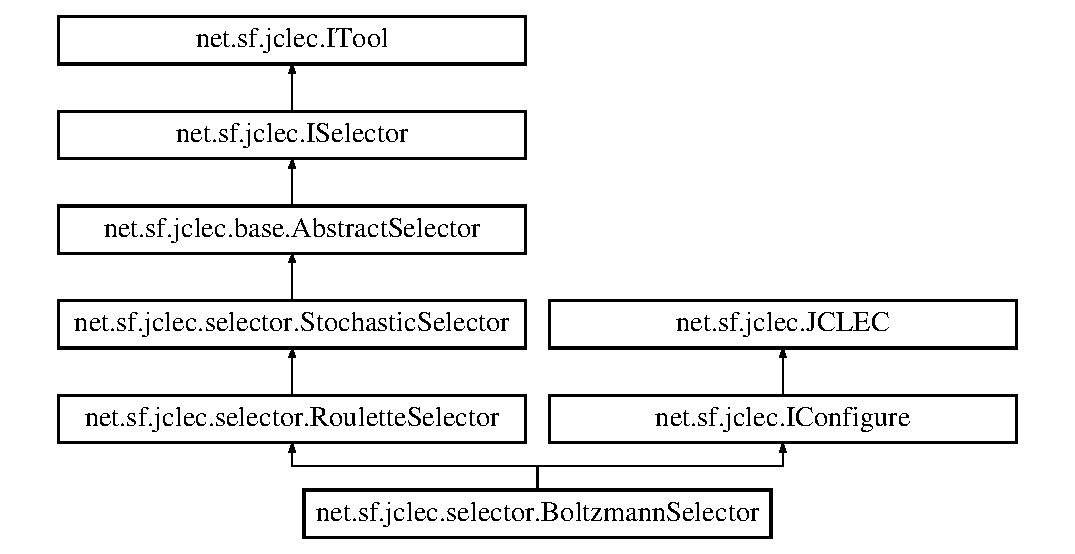
\includegraphics[height=6.000000cm]{classnet_1_1sf_1_1jclec_1_1selector_1_1_boltzmann_selector}
\end{center}
\end{figure}
\subsection*{Public Member Functions}
\begin{DoxyCompactItemize}
\item 
\hyperlink{classnet_1_1sf_1_1jclec_1_1selector_1_1_boltzmann_selector_a7ffc12fb7136454bab5790095287fd04}{Boltzmann\-Selector} ()
\item 
\hyperlink{classnet_1_1sf_1_1jclec_1_1selector_1_1_boltzmann_selector_a83bd891e99311359aa59172c90292920}{Boltzmann\-Selector} (\hyperlink{interfacenet_1_1sf_1_1jclec_1_1_i_system}{I\-System} \hyperlink{classnet_1_1sf_1_1jclec_1_1base_1_1_abstract_selector_a4304fe5c27aa7631dc91678d22473b94}{context})
\item 
double \hyperlink{classnet_1_1sf_1_1jclec_1_1selector_1_1_boltzmann_selector_a35d0f9ab6048f4be319efdfd26123c35}{get\-Initial\-Temp} ()
\item 
void \hyperlink{classnet_1_1sf_1_1jclec_1_1selector_1_1_boltzmann_selector_ac9fe1ead0fc07c2254163f283612213d}{set\-Initial\-Temp} (double initial\-Temp)
\item 
double \hyperlink{classnet_1_1sf_1_1jclec_1_1selector_1_1_boltzmann_selector_a5a30dfeedd870ac2b60c9aef5d44c277}{get\-Temp\-Decr} ()
\item 
void \hyperlink{classnet_1_1sf_1_1jclec_1_1selector_1_1_boltzmann_selector_a8e33ec0f1d3ff60baf42f4ae9d3994a9}{set\-Temp\-Decr} (double temp\-Decr)
\item 
void \hyperlink{classnet_1_1sf_1_1jclec_1_1selector_1_1_boltzmann_selector_a65e48d1e3e59775fffa2e2533f18537c}{configure} (Configuration configuration)
\end{DoxyCompactItemize}
\subsection*{Protected Member Functions}
\begin{DoxyCompactItemize}
\item 
void \hyperlink{classnet_1_1sf_1_1jclec_1_1selector_1_1_boltzmann_selector_a6edd0857b95771a97a1484b98ebc2fb0}{prepare\-Selection} ()
\item 
final void \hyperlink{classnet_1_1sf_1_1jclec_1_1selector_1_1_boltzmann_selector_a3436a5c3fa67afe7e1af7704841ab489}{update\-Temperature} ()
\end{DoxyCompactItemize}
\subsection*{Additional Inherited Members}


\subsection{Detailed Description}
Boltzmann Selector.

\begin{DoxyAuthor}{Author}
Sebastian Ventura 
\end{DoxyAuthor}


\subsection{Constructor \& Destructor Documentation}
\hypertarget{classnet_1_1sf_1_1jclec_1_1selector_1_1_boltzmann_selector_a7ffc12fb7136454bab5790095287fd04}{\index{net\-::sf\-::jclec\-::selector\-::\-Boltzmann\-Selector@{net\-::sf\-::jclec\-::selector\-::\-Boltzmann\-Selector}!Boltzmann\-Selector@{Boltzmann\-Selector}}
\index{Boltzmann\-Selector@{Boltzmann\-Selector}!net::sf::jclec::selector::BoltzmannSelector@{net\-::sf\-::jclec\-::selector\-::\-Boltzmann\-Selector}}
\subsubsection[{Boltzmann\-Selector}]{\setlength{\rightskip}{0pt plus 5cm}net.\-sf.\-jclec.\-selector.\-Boltzmann\-Selector.\-Boltzmann\-Selector (
\begin{DoxyParamCaption}
{}
\end{DoxyParamCaption}
)}}\label{classnet_1_1sf_1_1jclec_1_1selector_1_1_boltzmann_selector_a7ffc12fb7136454bab5790095287fd04}
Empty (default constructor). \hypertarget{classnet_1_1sf_1_1jclec_1_1selector_1_1_boltzmann_selector_a83bd891e99311359aa59172c90292920}{\index{net\-::sf\-::jclec\-::selector\-::\-Boltzmann\-Selector@{net\-::sf\-::jclec\-::selector\-::\-Boltzmann\-Selector}!Boltzmann\-Selector@{Boltzmann\-Selector}}
\index{Boltzmann\-Selector@{Boltzmann\-Selector}!net::sf::jclec::selector::BoltzmannSelector@{net\-::sf\-::jclec\-::selector\-::\-Boltzmann\-Selector}}
\subsubsection[{Boltzmann\-Selector}]{\setlength{\rightskip}{0pt plus 5cm}net.\-sf.\-jclec.\-selector.\-Boltzmann\-Selector.\-Boltzmann\-Selector (
\begin{DoxyParamCaption}
\item[{{\bf I\-System}}]{context}
\end{DoxyParamCaption}
)}}\label{classnet_1_1sf_1_1jclec_1_1selector_1_1_boltzmann_selector_a83bd891e99311359aa59172c90292920}
Constructor that contextualize selector


\begin{DoxyParams}{Parameters}
{\em context} & Execution context \\
\hline
\end{DoxyParams}


\subsection{Member Function Documentation}
\hypertarget{classnet_1_1sf_1_1jclec_1_1selector_1_1_boltzmann_selector_a65e48d1e3e59775fffa2e2533f18537c}{\index{net\-::sf\-::jclec\-::selector\-::\-Boltzmann\-Selector@{net\-::sf\-::jclec\-::selector\-::\-Boltzmann\-Selector}!configure@{configure}}
\index{configure@{configure}!net::sf::jclec::selector::BoltzmannSelector@{net\-::sf\-::jclec\-::selector\-::\-Boltzmann\-Selector}}
\subsubsection[{configure}]{\setlength{\rightskip}{0pt plus 5cm}void net.\-sf.\-jclec.\-selector.\-Boltzmann\-Selector.\-configure (
\begin{DoxyParamCaption}
\item[{Configuration}]{configuration}
\end{DoxyParamCaption}
)}}\label{classnet_1_1sf_1_1jclec_1_1selector_1_1_boltzmann_selector_a65e48d1e3e59775fffa2e2533f18537c}
Configuration method.


\begin{DoxyParams}{Parameters}
{\em settings} & Configuration settings\\
\hline
\end{DoxyParams}
 

Implements \hyperlink{interfacenet_1_1sf_1_1jclec_1_1_i_configure_add31a65a04d148c690a956fbbad6987c}{net.\-sf.\-jclec.\-I\-Configure}.

\hypertarget{classnet_1_1sf_1_1jclec_1_1selector_1_1_boltzmann_selector_a35d0f9ab6048f4be319efdfd26123c35}{\index{net\-::sf\-::jclec\-::selector\-::\-Boltzmann\-Selector@{net\-::sf\-::jclec\-::selector\-::\-Boltzmann\-Selector}!get\-Initial\-Temp@{get\-Initial\-Temp}}
\index{get\-Initial\-Temp@{get\-Initial\-Temp}!net::sf::jclec::selector::BoltzmannSelector@{net\-::sf\-::jclec\-::selector\-::\-Boltzmann\-Selector}}
\subsubsection[{get\-Initial\-Temp}]{\setlength{\rightskip}{0pt plus 5cm}double net.\-sf.\-jclec.\-selector.\-Boltzmann\-Selector.\-get\-Initial\-Temp (
\begin{DoxyParamCaption}
{}
\end{DoxyParamCaption}
)}}\label{classnet_1_1sf_1_1jclec_1_1selector_1_1_boltzmann_selector_a35d0f9ab6048f4be319efdfd26123c35}
Access to initial temperature.

\begin{DoxyReturn}{Returns}
Initial temperature 
\end{DoxyReturn}
\hypertarget{classnet_1_1sf_1_1jclec_1_1selector_1_1_boltzmann_selector_a5a30dfeedd870ac2b60c9aef5d44c277}{\index{net\-::sf\-::jclec\-::selector\-::\-Boltzmann\-Selector@{net\-::sf\-::jclec\-::selector\-::\-Boltzmann\-Selector}!get\-Temp\-Decr@{get\-Temp\-Decr}}
\index{get\-Temp\-Decr@{get\-Temp\-Decr}!net::sf::jclec::selector::BoltzmannSelector@{net\-::sf\-::jclec\-::selector\-::\-Boltzmann\-Selector}}
\subsubsection[{get\-Temp\-Decr}]{\setlength{\rightskip}{0pt plus 5cm}double net.\-sf.\-jclec.\-selector.\-Boltzmann\-Selector.\-get\-Temp\-Decr (
\begin{DoxyParamCaption}
{}
\end{DoxyParamCaption}
)}}\label{classnet_1_1sf_1_1jclec_1_1selector_1_1_boltzmann_selector_a5a30dfeedd870ac2b60c9aef5d44c277}
Acceso to temperature decrement constant.

\begin{DoxyReturn}{Returns}
Decrement temperature constant 
\end{DoxyReturn}
\hypertarget{classnet_1_1sf_1_1jclec_1_1selector_1_1_boltzmann_selector_a6edd0857b95771a97a1484b98ebc2fb0}{\index{net\-::sf\-::jclec\-::selector\-::\-Boltzmann\-Selector@{net\-::sf\-::jclec\-::selector\-::\-Boltzmann\-Selector}!prepare\-Selection@{prepare\-Selection}}
\index{prepare\-Selection@{prepare\-Selection}!net::sf::jclec::selector::BoltzmannSelector@{net\-::sf\-::jclec\-::selector\-::\-Boltzmann\-Selector}}
\subsubsection[{prepare\-Selection}]{\setlength{\rightskip}{0pt plus 5cm}void net.\-sf.\-jclec.\-selector.\-Boltzmann\-Selector.\-prepare\-Selection (
\begin{DoxyParamCaption}
{}
\end{DoxyParamCaption}
)\hspace{0.3cm}{\ttfamily [protected]}, {\ttfamily [virtual]}}}\label{classnet_1_1sf_1_1jclec_1_1selector_1_1_boltzmann_selector_a6edd0857b95771a97a1484b98ebc2fb0}
This phase performs ...


\begin{DoxyEnumerate}
\item Update temperature 
\item Set roulette values as exp(fitness/\-T) 
\item Normalize roulette value 
\end{DoxyEnumerate}

Prepare the selection process. 

Implements \hyperlink{classnet_1_1sf_1_1jclec_1_1base_1_1_abstract_selector_a0c5d9cb96fef9786e272b9edd811111e}{net.\-sf.\-jclec.\-base.\-Abstract\-Selector}.

\hypertarget{classnet_1_1sf_1_1jclec_1_1selector_1_1_boltzmann_selector_ac9fe1ead0fc07c2254163f283612213d}{\index{net\-::sf\-::jclec\-::selector\-::\-Boltzmann\-Selector@{net\-::sf\-::jclec\-::selector\-::\-Boltzmann\-Selector}!set\-Initial\-Temp@{set\-Initial\-Temp}}
\index{set\-Initial\-Temp@{set\-Initial\-Temp}!net::sf::jclec::selector::BoltzmannSelector@{net\-::sf\-::jclec\-::selector\-::\-Boltzmann\-Selector}}
\subsubsection[{set\-Initial\-Temp}]{\setlength{\rightskip}{0pt plus 5cm}void net.\-sf.\-jclec.\-selector.\-Boltzmann\-Selector.\-set\-Initial\-Temp (
\begin{DoxyParamCaption}
\item[{double}]{initial\-Temp}
\end{DoxyParamCaption}
)}}\label{classnet_1_1sf_1_1jclec_1_1selector_1_1_boltzmann_selector_ac9fe1ead0fc07c2254163f283612213d}
Sets initial temperature


\begin{DoxyParams}{Parameters}
{\em initial\-Temp} & Initial temperature value \\
\hline
\end{DoxyParams}
\hypertarget{classnet_1_1sf_1_1jclec_1_1selector_1_1_boltzmann_selector_a8e33ec0f1d3ff60baf42f4ae9d3994a9}{\index{net\-::sf\-::jclec\-::selector\-::\-Boltzmann\-Selector@{net\-::sf\-::jclec\-::selector\-::\-Boltzmann\-Selector}!set\-Temp\-Decr@{set\-Temp\-Decr}}
\index{set\-Temp\-Decr@{set\-Temp\-Decr}!net::sf::jclec::selector::BoltzmannSelector@{net\-::sf\-::jclec\-::selector\-::\-Boltzmann\-Selector}}
\subsubsection[{set\-Temp\-Decr}]{\setlength{\rightskip}{0pt plus 5cm}void net.\-sf.\-jclec.\-selector.\-Boltzmann\-Selector.\-set\-Temp\-Decr (
\begin{DoxyParamCaption}
\item[{double}]{temp\-Decr}
\end{DoxyParamCaption}
)}}\label{classnet_1_1sf_1_1jclec_1_1selector_1_1_boltzmann_selector_a8e33ec0f1d3ff60baf42f4ae9d3994a9}
Set decrement temperature constant


\begin{DoxyParams}{Parameters}
{\em temp\-Decr} & New temperature decrement constant \\
\hline
\end{DoxyParams}
\hypertarget{classnet_1_1sf_1_1jclec_1_1selector_1_1_boltzmann_selector_a3436a5c3fa67afe7e1af7704841ab489}{\index{net\-::sf\-::jclec\-::selector\-::\-Boltzmann\-Selector@{net\-::sf\-::jclec\-::selector\-::\-Boltzmann\-Selector}!update\-Temperature@{update\-Temperature}}
\index{update\-Temperature@{update\-Temperature}!net::sf::jclec::selector::BoltzmannSelector@{net\-::sf\-::jclec\-::selector\-::\-Boltzmann\-Selector}}
\subsubsection[{update\-Temperature}]{\setlength{\rightskip}{0pt plus 5cm}final void net.\-sf.\-jclec.\-selector.\-Boltzmann\-Selector.\-update\-Temperature (
\begin{DoxyParamCaption}
{}
\end{DoxyParamCaption}
)\hspace{0.3cm}{\ttfamily [protected]}}}\label{classnet_1_1sf_1_1jclec_1_1selector_1_1_boltzmann_selector_a3436a5c3fa67afe7e1af7704841ab489}
Update temperature 

The documentation for this class was generated from the following file\-:\begin{DoxyCompactItemize}
\item 
src/main/java/net/sf/jclec/selector/Boltzmann\-Selector.\-java\end{DoxyCompactItemize}

\hypertarget{classnet_1_1sf_1_1jclec_1_1algorithm_1_1classic_1_1_c_h_c}{\section{net.\-sf.\-jclec.\-algorithm.\-classic.\-C\-H\-C Class Reference}
\label{classnet_1_1sf_1_1jclec_1_1algorithm_1_1classic_1_1_c_h_c}\index{net.\-sf.\-jclec.\-algorithm.\-classic.\-C\-H\-C@{net.\-sf.\-jclec.\-algorithm.\-classic.\-C\-H\-C}}
}
Inheritance diagram for net.\-sf.\-jclec.\-algorithm.\-classic.\-C\-H\-C\-:\begin{figure}[H]
\begin{center}
\leavevmode
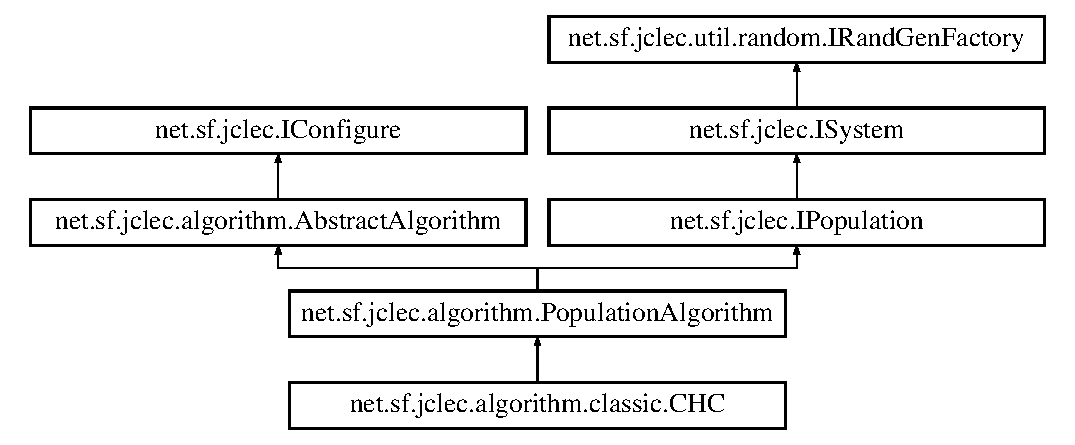
\includegraphics[height=5.000000cm]{classnet_1_1sf_1_1jclec_1_1algorithm_1_1classic_1_1_c_h_c}
\end{center}
\end{figure}
\subsection*{Public Member Functions}
\begin{DoxyCompactItemize}
\item 
\hyperlink{classnet_1_1sf_1_1jclec_1_1algorithm_1_1classic_1_1_c_h_c_a4729dc96519b67a9ae66ddedd03847b4}{C\-H\-C} ()
\item 
void \hyperlink{classnet_1_1sf_1_1jclec_1_1algorithm_1_1classic_1_1_c_h_c_ad67660256f71edbc94359158049140b5}{set\-Rand\-Gen\-Factory} (\hyperlink{interfacenet_1_1sf_1_1jclec_1_1util_1_1random_1_1_i_rand_gen_factory}{I\-Rand\-Gen\-Factory} \hyperlink{classnet_1_1sf_1_1jclec_1_1algorithm_1_1_population_algorithm_a8cb8eb8086086a7ddd879f8e0c1468d7}{rand\-Gen\-Factory})
\item 
int \hyperlink{classnet_1_1sf_1_1jclec_1_1algorithm_1_1classic_1_1_c_h_c_affa00f6d4ac6082f31a2f9add3cf138d}{get\-Initial\-D} ()
\item 
void \hyperlink{classnet_1_1sf_1_1jclec_1_1algorithm_1_1classic_1_1_c_h_c_ac898e18ad4b2a2dcd655a275ef0a7f6c}{set\-Initial\-D} (int \hyperlink{classnet_1_1sf_1_1jclec_1_1algorithm_1_1classic_1_1_c_h_c_a4b7c785a6c035901c27655736802f1d5}{initial\-D})
\item 
\hyperlink{interfacenet_1_1sf_1_1jclec_1_1_i_distance}{I\-Distance} \hyperlink{classnet_1_1sf_1_1jclec_1_1algorithm_1_1classic_1_1_c_h_c_aaaea1616cfd0bfd5bd049936c189e266}{get\-Distance} ()
\item 
void \hyperlink{classnet_1_1sf_1_1jclec_1_1algorithm_1_1classic_1_1_c_h_c_aaab3b5ede7b5650bbb5b1f51532656b7}{set\-Distance} (\hyperlink{interfacenet_1_1sf_1_1jclec_1_1_i_distance}{I\-Distance} \hyperlink{classnet_1_1sf_1_1jclec_1_1algorithm_1_1classic_1_1_c_h_c_af5aede7c9435b3e8d6826e880c7247dc}{distance})
\item 
\hyperlink{interfacenet_1_1sf_1_1jclec_1_1_i_recombinator}{I\-Recombinator} \hyperlink{classnet_1_1sf_1_1jclec_1_1algorithm_1_1classic_1_1_c_h_c_a039c94fe5c17aba606cb794dacd9ae7c}{get\-Recombinator} ()
\item 
void \hyperlink{classnet_1_1sf_1_1jclec_1_1algorithm_1_1classic_1_1_c_h_c_a775859e89f9dab908522cb00aabf5e7f}{set\-Recombinator} (\hyperlink{interfacenet_1_1sf_1_1jclec_1_1_i_recombinator}{I\-Recombinator} \hyperlink{classnet_1_1sf_1_1jclec_1_1algorithm_1_1classic_1_1_c_h_c_ab57efc757b80ad7047b60477e7329718}{recombinator})
\item 
int \hyperlink{classnet_1_1sf_1_1jclec_1_1algorithm_1_1classic_1_1_c_h_c_a0e46f9df67ccf3ab215c5be86cb30bc1}{get\-Restart\-D} ()
\item 
void \hyperlink{classnet_1_1sf_1_1jclec_1_1algorithm_1_1classic_1_1_c_h_c_a016cf9538a31a771aa2c1b3f026cd4af}{set\-Restart\-D} (int \hyperlink{classnet_1_1sf_1_1jclec_1_1algorithm_1_1classic_1_1_c_h_c_a6cd78db6a675d92c105ee5e4cf5abe68}{restart\-D})
\item 
int \hyperlink{classnet_1_1sf_1_1jclec_1_1algorithm_1_1classic_1_1_c_h_c_a7c43670824769e5a587a553651139ae2}{get\-Number\-Of\-Survidors} ()
\item 
void \hyperlink{classnet_1_1sf_1_1jclec_1_1algorithm_1_1classic_1_1_c_h_c_adda9d489762695605817a0cb70773db4}{set\-Number\-Of\-Survivors} (int \hyperlink{classnet_1_1sf_1_1jclec_1_1algorithm_1_1classic_1_1_c_h_c_a1b2005c9606fa0bd250efda96aa078d9}{number\-Of\-Survivors})
\item 
\hyperlink{interfacenet_1_1sf_1_1jclec_1_1_i_mutator}{I\-Mutator} \hyperlink{classnet_1_1sf_1_1jclec_1_1algorithm_1_1classic_1_1_c_h_c_aa238175b12ebb189aafe64e9ccb5f0db}{get\-Mutator} ()
\item 
void \hyperlink{classnet_1_1sf_1_1jclec_1_1algorithm_1_1classic_1_1_c_h_c_ab29cf3fb56310cdbef735eed330d03c6}{set\-Mutator} (\hyperlink{interfacenet_1_1sf_1_1jclec_1_1_i_mutator}{I\-Mutator} \hyperlink{classnet_1_1sf_1_1jclec_1_1algorithm_1_1classic_1_1_c_h_c_adfd26c19f5be720ec4dc4199b99cdf96}{mutator})
\item 
void \hyperlink{classnet_1_1sf_1_1jclec_1_1algorithm_1_1classic_1_1_c_h_c_aa7f07c25bf43054348667de877ba4b2e}{configure} (Configuration configuration)
\end{DoxyCompactItemize}
\subsection*{Protected Member Functions}
\begin{DoxyCompactItemize}
\item 
void \hyperlink{classnet_1_1sf_1_1jclec_1_1algorithm_1_1classic_1_1_c_h_c_aa707ae364027caf08eba0499fc310efe}{do\-Init} ()
\item 
void \hyperlink{classnet_1_1sf_1_1jclec_1_1algorithm_1_1classic_1_1_c_h_c_a8e0ae8b8e6537421347a28eb8c8bc039}{do\-Selection} ()
\item 
void \hyperlink{classnet_1_1sf_1_1jclec_1_1algorithm_1_1classic_1_1_c_h_c_ac5e50e91baa147c263dd73e039aa10e1}{do\-Generation} ()
\item 
void \hyperlink{classnet_1_1sf_1_1jclec_1_1algorithm_1_1classic_1_1_c_h_c_a4ccfdb444710b853f4a8dfeed86e7b8b}{do\-Replacement} ()
\item 
void \hyperlink{classnet_1_1sf_1_1jclec_1_1algorithm_1_1classic_1_1_c_h_c_a3e4179196cc7577862038e2355471d04}{do\-Update} ()
\end{DoxyCompactItemize}
\subsection*{Protected Attributes}
\begin{DoxyCompactItemize}
\item 
int \hyperlink{classnet_1_1sf_1_1jclec_1_1algorithm_1_1classic_1_1_c_h_c_a4b7c785a6c035901c27655736802f1d5}{initial\-D}
\item 
\hyperlink{interfacenet_1_1sf_1_1jclec_1_1_i_distance}{I\-Distance} \hyperlink{classnet_1_1sf_1_1jclec_1_1algorithm_1_1classic_1_1_c_h_c_af5aede7c9435b3e8d6826e880c7247dc}{distance}
\item 
\hyperlink{interfacenet_1_1sf_1_1jclec_1_1_i_recombinator}{I\-Recombinator} \hyperlink{classnet_1_1sf_1_1jclec_1_1algorithm_1_1classic_1_1_c_h_c_ab57efc757b80ad7047b60477e7329718}{recombinator}
\item 
int \hyperlink{classnet_1_1sf_1_1jclec_1_1algorithm_1_1classic_1_1_c_h_c_a6cd78db6a675d92c105ee5e4cf5abe68}{restart\-D}
\item 
int \hyperlink{classnet_1_1sf_1_1jclec_1_1algorithm_1_1classic_1_1_c_h_c_a1b2005c9606fa0bd250efda96aa078d9}{number\-Of\-Survivors}
\item 
\hyperlink{interfacenet_1_1sf_1_1jclec_1_1_i_mutator}{I\-Mutator} \hyperlink{classnet_1_1sf_1_1jclec_1_1algorithm_1_1classic_1_1_c_h_c_adfd26c19f5be720ec4dc4199b99cdf96}{mutator}
\end{DoxyCompactItemize}


\subsection{Detailed Description}
\hyperlink{classnet_1_1sf_1_1jclec_1_1algorithm_1_1classic_1_1_c_h_c}{C\-H\-C} algorithm. This implementation allows non-\/binary individuals. To do that, user has to define the distance to use in the incest prevention phase, as well as the recombinator to use in the generation phase and the mutator to use in the restarting phase (optional).

\begin{DoxyAuthor}{Author}
Sebastian Ventura 
\end{DoxyAuthor}


\subsection{Constructor \& Destructor Documentation}
\hypertarget{classnet_1_1sf_1_1jclec_1_1algorithm_1_1classic_1_1_c_h_c_a4729dc96519b67a9ae66ddedd03847b4}{\index{net\-::sf\-::jclec\-::algorithm\-::classic\-::\-C\-H\-C@{net\-::sf\-::jclec\-::algorithm\-::classic\-::\-C\-H\-C}!C\-H\-C@{C\-H\-C}}
\index{C\-H\-C@{C\-H\-C}!net::sf::jclec::algorithm::classic::CHC@{net\-::sf\-::jclec\-::algorithm\-::classic\-::\-C\-H\-C}}
\subsubsection[{C\-H\-C}]{\setlength{\rightskip}{0pt plus 5cm}net.\-sf.\-jclec.\-algorithm.\-classic.\-C\-H\-C.\-C\-H\-C (
\begin{DoxyParamCaption}
{}
\end{DoxyParamCaption}
)}}\label{classnet_1_1sf_1_1jclec_1_1algorithm_1_1classic_1_1_c_h_c_a4729dc96519b67a9ae66ddedd03847b4}
Empty (default) constructor 

\subsection{Member Function Documentation}
\hypertarget{classnet_1_1sf_1_1jclec_1_1algorithm_1_1classic_1_1_c_h_c_aa7f07c25bf43054348667de877ba4b2e}{\index{net\-::sf\-::jclec\-::algorithm\-::classic\-::\-C\-H\-C@{net\-::sf\-::jclec\-::algorithm\-::classic\-::\-C\-H\-C}!configure@{configure}}
\index{configure@{configure}!net::sf::jclec::algorithm::classic::CHC@{net\-::sf\-::jclec\-::algorithm\-::classic\-::\-C\-H\-C}}
\subsubsection[{configure}]{\setlength{\rightskip}{0pt plus 5cm}void net.\-sf.\-jclec.\-algorithm.\-classic.\-C\-H\-C.\-configure (
\begin{DoxyParamCaption}
\item[{Configuration}]{configuration}
\end{DoxyParamCaption}
)}}\label{classnet_1_1sf_1_1jclec_1_1algorithm_1_1classic_1_1_c_h_c_aa7f07c25bf43054348667de877ba4b2e}
Configuration method.


\begin{DoxyParams}{Parameters}
{\em settings} & Configuration settings\\
\hline
\end{DoxyParams}
 

Implements \hyperlink{interfacenet_1_1sf_1_1jclec_1_1_i_configure_add31a65a04d148c690a956fbbad6987c}{net.\-sf.\-jclec.\-I\-Configure}.

\hypertarget{classnet_1_1sf_1_1jclec_1_1algorithm_1_1classic_1_1_c_h_c_ac5e50e91baa147c263dd73e039aa10e1}{\index{net\-::sf\-::jclec\-::algorithm\-::classic\-::\-C\-H\-C@{net\-::sf\-::jclec\-::algorithm\-::classic\-::\-C\-H\-C}!do\-Generation@{do\-Generation}}
\index{do\-Generation@{do\-Generation}!net::sf::jclec::algorithm::classic::CHC@{net\-::sf\-::jclec\-::algorithm\-::classic\-::\-C\-H\-C}}
\subsubsection[{do\-Generation}]{\setlength{\rightskip}{0pt plus 5cm}void net.\-sf.\-jclec.\-algorithm.\-classic.\-C\-H\-C.\-do\-Generation (
\begin{DoxyParamCaption}
{}
\end{DoxyParamCaption}
)\hspace{0.3cm}{\ttfamily [protected]}, {\ttfamily [virtual]}}}\label{classnet_1_1sf_1_1jclec_1_1algorithm_1_1classic_1_1_c_h_c_ac5e50e91baa147c263dd73e039aa10e1}
Apply recombinator over parents 

Implements \hyperlink{classnet_1_1sf_1_1jclec_1_1algorithm_1_1_population_algorithm_a04894ec2d7f9e72eca1a41127bd1c7d3}{net.\-sf.\-jclec.\-algorithm.\-Population\-Algorithm}.

\hypertarget{classnet_1_1sf_1_1jclec_1_1algorithm_1_1classic_1_1_c_h_c_aa707ae364027caf08eba0499fc310efe}{\index{net\-::sf\-::jclec\-::algorithm\-::classic\-::\-C\-H\-C@{net\-::sf\-::jclec\-::algorithm\-::classic\-::\-C\-H\-C}!do\-Init@{do\-Init}}
\index{do\-Init@{do\-Init}!net::sf::jclec::algorithm::classic::CHC@{net\-::sf\-::jclec\-::algorithm\-::classic\-::\-C\-H\-C}}
\subsubsection[{do\-Init}]{\setlength{\rightskip}{0pt plus 5cm}void net.\-sf.\-jclec.\-algorithm.\-classic.\-C\-H\-C.\-do\-Init (
\begin{DoxyParamCaption}
{}
\end{DoxyParamCaption}
)\hspace{0.3cm}{\ttfamily [protected]}, {\ttfamily [virtual]}}}\label{classnet_1_1sf_1_1jclec_1_1algorithm_1_1classic_1_1_c_h_c_aa707ae364027caf08eba0499fc310efe}
Call super.\-do\-Init(), then initialize d value

Perform algorithm initialization. 

Implements \hyperlink{classnet_1_1sf_1_1jclec_1_1algorithm_1_1_abstract_algorithm_a9cb5c0abb0c171944290260eccbc0078}{net.\-sf.\-jclec.\-algorithm.\-Abstract\-Algorithm}.

\hypertarget{classnet_1_1sf_1_1jclec_1_1algorithm_1_1classic_1_1_c_h_c_a4ccfdb444710b853f4a8dfeed86e7b8b}{\index{net\-::sf\-::jclec\-::algorithm\-::classic\-::\-C\-H\-C@{net\-::sf\-::jclec\-::algorithm\-::classic\-::\-C\-H\-C}!do\-Replacement@{do\-Replacement}}
\index{do\-Replacement@{do\-Replacement}!net::sf::jclec::algorithm::classic::CHC@{net\-::sf\-::jclec\-::algorithm\-::classic\-::\-C\-H\-C}}
\subsubsection[{do\-Replacement}]{\setlength{\rightskip}{0pt plus 5cm}void net.\-sf.\-jclec.\-algorithm.\-classic.\-C\-H\-C.\-do\-Replacement (
\begin{DoxyParamCaption}
{}
\end{DoxyParamCaption}
)\hspace{0.3cm}{\ttfamily [protected]}, {\ttfamily [virtual]}}}\label{classnet_1_1sf_1_1jclec_1_1algorithm_1_1classic_1_1_c_h_c_a4ccfdb444710b853f4a8dfeed86e7b8b}
Do nothing 

Implements \hyperlink{classnet_1_1sf_1_1jclec_1_1algorithm_1_1_population_algorithm_afac7f83430707d572fbe8a2ea79c3685}{net.\-sf.\-jclec.\-algorithm.\-Population\-Algorithm}.

\hypertarget{classnet_1_1sf_1_1jclec_1_1algorithm_1_1classic_1_1_c_h_c_a8e0ae8b8e6537421347a28eb8c8bc039}{\index{net\-::sf\-::jclec\-::algorithm\-::classic\-::\-C\-H\-C@{net\-::sf\-::jclec\-::algorithm\-::classic\-::\-C\-H\-C}!do\-Selection@{do\-Selection}}
\index{do\-Selection@{do\-Selection}!net::sf::jclec::algorithm::classic::CHC@{net\-::sf\-::jclec\-::algorithm\-::classic\-::\-C\-H\-C}}
\subsubsection[{do\-Selection}]{\setlength{\rightskip}{0pt plus 5cm}void net.\-sf.\-jclec.\-algorithm.\-classic.\-C\-H\-C.\-do\-Selection (
\begin{DoxyParamCaption}
{}
\end{DoxyParamCaption}
)\hspace{0.3cm}{\ttfamily [protected]}, {\ttfamily [virtual]}}}\label{classnet_1_1sf_1_1jclec_1_1algorithm_1_1classic_1_1_c_h_c_a8e0ae8b8e6537421347a28eb8c8bc039}
Shuffle individuals in bset, then prevents individuals incest 

Implements \hyperlink{classnet_1_1sf_1_1jclec_1_1algorithm_1_1_population_algorithm_a0c3b482671dc8c454f968a30a374c3be}{net.\-sf.\-jclec.\-algorithm.\-Population\-Algorithm}.

\hypertarget{classnet_1_1sf_1_1jclec_1_1algorithm_1_1classic_1_1_c_h_c_a3e4179196cc7577862038e2355471d04}{\index{net\-::sf\-::jclec\-::algorithm\-::classic\-::\-C\-H\-C@{net\-::sf\-::jclec\-::algorithm\-::classic\-::\-C\-H\-C}!do\-Update@{do\-Update}}
\index{do\-Update@{do\-Update}!net::sf::jclec::algorithm::classic::CHC@{net\-::sf\-::jclec\-::algorithm\-::classic\-::\-C\-H\-C}}
\subsubsection[{do\-Update}]{\setlength{\rightskip}{0pt plus 5cm}void net.\-sf.\-jclec.\-algorithm.\-classic.\-C\-H\-C.\-do\-Update (
\begin{DoxyParamCaption}
{}
\end{DoxyParamCaption}
)\hspace{0.3cm}{\ttfamily [protected]}, {\ttfamily [virtual]}}}\label{classnet_1_1sf_1_1jclec_1_1algorithm_1_1classic_1_1_c_h_c_a3e4179196cc7577862038e2355471d04}
This method includes the following actions\-:


\begin{DoxyItemize}
\item Check whether recombination was successful. If so, return new population 
\item If recombination was not successful, update d parameter 
\item If d parameter is negative, performs restart 
\end{DoxyItemize}

Implements \hyperlink{classnet_1_1sf_1_1jclec_1_1algorithm_1_1_population_algorithm_a0817186f210c38255cc46f490cbbf53e}{net.\-sf.\-jclec.\-algorithm.\-Population\-Algorithm}.

\hypertarget{classnet_1_1sf_1_1jclec_1_1algorithm_1_1classic_1_1_c_h_c_aaaea1616cfd0bfd5bd049936c189e266}{\index{net\-::sf\-::jclec\-::algorithm\-::classic\-::\-C\-H\-C@{net\-::sf\-::jclec\-::algorithm\-::classic\-::\-C\-H\-C}!get\-Distance@{get\-Distance}}
\index{get\-Distance@{get\-Distance}!net::sf::jclec::algorithm::classic::CHC@{net\-::sf\-::jclec\-::algorithm\-::classic\-::\-C\-H\-C}}
\subsubsection[{get\-Distance}]{\setlength{\rightskip}{0pt plus 5cm}{\bf I\-Distance} net.\-sf.\-jclec.\-algorithm.\-classic.\-C\-H\-C.\-get\-Distance (
\begin{DoxyParamCaption}
{}
\end{DoxyParamCaption}
)}}\label{classnet_1_1sf_1_1jclec_1_1algorithm_1_1classic_1_1_c_h_c_aaaea1616cfd0bfd5bd049936c189e266}
Access to distance between individuals. This distance is used in the 'incest prevention' phase.

\begin{DoxyReturn}{Returns}
Distance used at incest prevention phase 
\end{DoxyReturn}
\hypertarget{classnet_1_1sf_1_1jclec_1_1algorithm_1_1classic_1_1_c_h_c_affa00f6d4ac6082f31a2f9add3cf138d}{\index{net\-::sf\-::jclec\-::algorithm\-::classic\-::\-C\-H\-C@{net\-::sf\-::jclec\-::algorithm\-::classic\-::\-C\-H\-C}!get\-Initial\-D@{get\-Initial\-D}}
\index{get\-Initial\-D@{get\-Initial\-D}!net::sf::jclec::algorithm::classic::CHC@{net\-::sf\-::jclec\-::algorithm\-::classic\-::\-C\-H\-C}}
\subsubsection[{get\-Initial\-D}]{\setlength{\rightskip}{0pt plus 5cm}int net.\-sf.\-jclec.\-algorithm.\-classic.\-C\-H\-C.\-get\-Initial\-D (
\begin{DoxyParamCaption}
{}
\end{DoxyParamCaption}
)}}\label{classnet_1_1sf_1_1jclec_1_1algorithm_1_1classic_1_1_c_h_c_affa00f6d4ac6082f31a2f9add3cf138d}
Access to initial D

\begin{DoxyReturn}{Returns}
Initial D 
\end{DoxyReturn}
\hypertarget{classnet_1_1sf_1_1jclec_1_1algorithm_1_1classic_1_1_c_h_c_aa238175b12ebb189aafe64e9ccb5f0db}{\index{net\-::sf\-::jclec\-::algorithm\-::classic\-::\-C\-H\-C@{net\-::sf\-::jclec\-::algorithm\-::classic\-::\-C\-H\-C}!get\-Mutator@{get\-Mutator}}
\index{get\-Mutator@{get\-Mutator}!net::sf::jclec::algorithm::classic::CHC@{net\-::sf\-::jclec\-::algorithm\-::classic\-::\-C\-H\-C}}
\subsubsection[{get\-Mutator}]{\setlength{\rightskip}{0pt plus 5cm}{\bf I\-Mutator} net.\-sf.\-jclec.\-algorithm.\-classic.\-C\-H\-C.\-get\-Mutator (
\begin{DoxyParamCaption}
{}
\end{DoxyParamCaption}
)}}\label{classnet_1_1sf_1_1jclec_1_1algorithm_1_1classic_1_1_c_h_c_aa238175b12ebb189aafe64e9ccb5f0db}
Access to mutator used in restarting

\begin{DoxyReturn}{Returns}
Restating mutator 
\end{DoxyReturn}
\hypertarget{classnet_1_1sf_1_1jclec_1_1algorithm_1_1classic_1_1_c_h_c_a7c43670824769e5a587a553651139ae2}{\index{net\-::sf\-::jclec\-::algorithm\-::classic\-::\-C\-H\-C@{net\-::sf\-::jclec\-::algorithm\-::classic\-::\-C\-H\-C}!get\-Number\-Of\-Survidors@{get\-Number\-Of\-Survidors}}
\index{get\-Number\-Of\-Survidors@{get\-Number\-Of\-Survidors}!net::sf::jclec::algorithm::classic::CHC@{net\-::sf\-::jclec\-::algorithm\-::classic\-::\-C\-H\-C}}
\subsubsection[{get\-Number\-Of\-Survidors}]{\setlength{\rightskip}{0pt plus 5cm}int net.\-sf.\-jclec.\-algorithm.\-classic.\-C\-H\-C.\-get\-Number\-Of\-Survidors (
\begin{DoxyParamCaption}
{}
\end{DoxyParamCaption}
)}}\label{classnet_1_1sf_1_1jclec_1_1algorithm_1_1classic_1_1_c_h_c_a7c43670824769e5a587a553651139ae2}
Number of survivors after restarting

\begin{DoxyReturn}{Returns}
Number of survivors after restarting 
\end{DoxyReturn}
\hypertarget{classnet_1_1sf_1_1jclec_1_1algorithm_1_1classic_1_1_c_h_c_a039c94fe5c17aba606cb794dacd9ae7c}{\index{net\-::sf\-::jclec\-::algorithm\-::classic\-::\-C\-H\-C@{net\-::sf\-::jclec\-::algorithm\-::classic\-::\-C\-H\-C}!get\-Recombinator@{get\-Recombinator}}
\index{get\-Recombinator@{get\-Recombinator}!net::sf::jclec::algorithm::classic::CHC@{net\-::sf\-::jclec\-::algorithm\-::classic\-::\-C\-H\-C}}
\subsubsection[{get\-Recombinator}]{\setlength{\rightskip}{0pt plus 5cm}{\bf I\-Recombinator} net.\-sf.\-jclec.\-algorithm.\-classic.\-C\-H\-C.\-get\-Recombinator (
\begin{DoxyParamCaption}
{}
\end{DoxyParamCaption}
)}}\label{classnet_1_1sf_1_1jclec_1_1algorithm_1_1classic_1_1_c_h_c_a039c94fe5c17aba606cb794dacd9ae7c}
Access to individuals recombinator

\begin{DoxyReturn}{Returns}
Individuals recombinator 
\end{DoxyReturn}
\hypertarget{classnet_1_1sf_1_1jclec_1_1algorithm_1_1classic_1_1_c_h_c_a0e46f9df67ccf3ab215c5be86cb30bc1}{\index{net\-::sf\-::jclec\-::algorithm\-::classic\-::\-C\-H\-C@{net\-::sf\-::jclec\-::algorithm\-::classic\-::\-C\-H\-C}!get\-Restart\-D@{get\-Restart\-D}}
\index{get\-Restart\-D@{get\-Restart\-D}!net::sf::jclec::algorithm::classic::CHC@{net\-::sf\-::jclec\-::algorithm\-::classic\-::\-C\-H\-C}}
\subsubsection[{get\-Restart\-D}]{\setlength{\rightskip}{0pt plus 5cm}int net.\-sf.\-jclec.\-algorithm.\-classic.\-C\-H\-C.\-get\-Restart\-D (
\begin{DoxyParamCaption}
{}
\end{DoxyParamCaption}
)}}\label{classnet_1_1sf_1_1jclec_1_1algorithm_1_1classic_1_1_c_h_c_a0e46f9df67ccf3ab215c5be86cb30bc1}
Access to D value for restart

\begin{DoxyReturn}{Returns}
D value for restart 
\end{DoxyReturn}
\hypertarget{classnet_1_1sf_1_1jclec_1_1algorithm_1_1classic_1_1_c_h_c_aaab3b5ede7b5650bbb5b1f51532656b7}{\index{net\-::sf\-::jclec\-::algorithm\-::classic\-::\-C\-H\-C@{net\-::sf\-::jclec\-::algorithm\-::classic\-::\-C\-H\-C}!set\-Distance@{set\-Distance}}
\index{set\-Distance@{set\-Distance}!net::sf::jclec::algorithm::classic::CHC@{net\-::sf\-::jclec\-::algorithm\-::classic\-::\-C\-H\-C}}
\subsubsection[{set\-Distance}]{\setlength{\rightskip}{0pt plus 5cm}void net.\-sf.\-jclec.\-algorithm.\-classic.\-C\-H\-C.\-set\-Distance (
\begin{DoxyParamCaption}
\item[{{\bf I\-Distance}}]{distance}
\end{DoxyParamCaption}
)}}\label{classnet_1_1sf_1_1jclec_1_1algorithm_1_1classic_1_1_c_h_c_aaab3b5ede7b5650bbb5b1f51532656b7}
Sets the distance to use in the 'incest prevention' phase.


\begin{DoxyParams}{Parameters}
{\em distance} & New distance \\
\hline
\end{DoxyParams}
\hypertarget{classnet_1_1sf_1_1jclec_1_1algorithm_1_1classic_1_1_c_h_c_ac898e18ad4b2a2dcd655a275ef0a7f6c}{\index{net\-::sf\-::jclec\-::algorithm\-::classic\-::\-C\-H\-C@{net\-::sf\-::jclec\-::algorithm\-::classic\-::\-C\-H\-C}!set\-Initial\-D@{set\-Initial\-D}}
\index{set\-Initial\-D@{set\-Initial\-D}!net::sf::jclec::algorithm::classic::CHC@{net\-::sf\-::jclec\-::algorithm\-::classic\-::\-C\-H\-C}}
\subsubsection[{set\-Initial\-D}]{\setlength{\rightskip}{0pt plus 5cm}void net.\-sf.\-jclec.\-algorithm.\-classic.\-C\-H\-C.\-set\-Initial\-D (
\begin{DoxyParamCaption}
\item[{int}]{initial\-D}
\end{DoxyParamCaption}
)}}\label{classnet_1_1sf_1_1jclec_1_1algorithm_1_1classic_1_1_c_h_c_ac898e18ad4b2a2dcd655a275ef0a7f6c}
Set initial D


\begin{DoxyParams}{Parameters}
{\em initial\-D} & Initial D \\
\hline
\end{DoxyParams}
\hypertarget{classnet_1_1sf_1_1jclec_1_1algorithm_1_1classic_1_1_c_h_c_ab29cf3fb56310cdbef735eed330d03c6}{\index{net\-::sf\-::jclec\-::algorithm\-::classic\-::\-C\-H\-C@{net\-::sf\-::jclec\-::algorithm\-::classic\-::\-C\-H\-C}!set\-Mutator@{set\-Mutator}}
\index{set\-Mutator@{set\-Mutator}!net::sf::jclec::algorithm::classic::CHC@{net\-::sf\-::jclec\-::algorithm\-::classic\-::\-C\-H\-C}}
\subsubsection[{set\-Mutator}]{\setlength{\rightskip}{0pt plus 5cm}void net.\-sf.\-jclec.\-algorithm.\-classic.\-C\-H\-C.\-set\-Mutator (
\begin{DoxyParamCaption}
\item[{{\bf I\-Mutator}}]{mutator}
\end{DoxyParamCaption}
)}}\label{classnet_1_1sf_1_1jclec_1_1algorithm_1_1classic_1_1_c_h_c_ab29cf3fb56310cdbef735eed330d03c6}
Sets the mutator used in restarting


\begin{DoxyParams}{Parameters}
{\em mutator} & Mutator used in restarting \\
\hline
\end{DoxyParams}
\hypertarget{classnet_1_1sf_1_1jclec_1_1algorithm_1_1classic_1_1_c_h_c_adda9d489762695605817a0cb70773db4}{\index{net\-::sf\-::jclec\-::algorithm\-::classic\-::\-C\-H\-C@{net\-::sf\-::jclec\-::algorithm\-::classic\-::\-C\-H\-C}!set\-Number\-Of\-Survivors@{set\-Number\-Of\-Survivors}}
\index{set\-Number\-Of\-Survivors@{set\-Number\-Of\-Survivors}!net::sf::jclec::algorithm::classic::CHC@{net\-::sf\-::jclec\-::algorithm\-::classic\-::\-C\-H\-C}}
\subsubsection[{set\-Number\-Of\-Survivors}]{\setlength{\rightskip}{0pt plus 5cm}void net.\-sf.\-jclec.\-algorithm.\-classic.\-C\-H\-C.\-set\-Number\-Of\-Survivors (
\begin{DoxyParamCaption}
\item[{int}]{number\-Of\-Survivors}
\end{DoxyParamCaption}
)}}\label{classnet_1_1sf_1_1jclec_1_1algorithm_1_1classic_1_1_c_h_c_adda9d489762695605817a0cb70773db4}
Sets the number of individuals that survive after restarting


\begin{DoxyParams}{Parameters}
{\em number\-Of\-Survivors} & Number of survivors \\
\hline
\end{DoxyParams}
\hypertarget{classnet_1_1sf_1_1jclec_1_1algorithm_1_1classic_1_1_c_h_c_ad67660256f71edbc94359158049140b5}{\index{net\-::sf\-::jclec\-::algorithm\-::classic\-::\-C\-H\-C@{net\-::sf\-::jclec\-::algorithm\-::classic\-::\-C\-H\-C}!set\-Rand\-Gen\-Factory@{set\-Rand\-Gen\-Factory}}
\index{set\-Rand\-Gen\-Factory@{set\-Rand\-Gen\-Factory}!net::sf::jclec::algorithm::classic::CHC@{net\-::sf\-::jclec\-::algorithm\-::classic\-::\-C\-H\-C}}
\subsubsection[{set\-Rand\-Gen\-Factory}]{\setlength{\rightskip}{0pt plus 5cm}void net.\-sf.\-jclec.\-algorithm.\-classic.\-C\-H\-C.\-set\-Rand\-Gen\-Factory (
\begin{DoxyParamCaption}
\item[{{\bf I\-Rand\-Gen\-Factory}}]{rand\-Gen\-Factory}
\end{DoxyParamCaption}
)}}\label{classnet_1_1sf_1_1jclec_1_1algorithm_1_1classic_1_1_c_h_c_ad67660256f71edbc94359158049140b5}
Once the rand\-Gen\-Factory has been set, set the random generator used to shuffle indviduals in selection phase.\hypertarget{classnet_1_1sf_1_1jclec_1_1algorithm_1_1classic_1_1_c_h_c_a775859e89f9dab908522cb00aabf5e7f}{\index{net\-::sf\-::jclec\-::algorithm\-::classic\-::\-C\-H\-C@{net\-::sf\-::jclec\-::algorithm\-::classic\-::\-C\-H\-C}!set\-Recombinator@{set\-Recombinator}}
\index{set\-Recombinator@{set\-Recombinator}!net::sf::jclec::algorithm::classic::CHC@{net\-::sf\-::jclec\-::algorithm\-::classic\-::\-C\-H\-C}}
\subsubsection[{set\-Recombinator}]{\setlength{\rightskip}{0pt plus 5cm}void net.\-sf.\-jclec.\-algorithm.\-classic.\-C\-H\-C.\-set\-Recombinator (
\begin{DoxyParamCaption}
\item[{{\bf I\-Recombinator}}]{recombinator}
\end{DoxyParamCaption}
)}}\label{classnet_1_1sf_1_1jclec_1_1algorithm_1_1classic_1_1_c_h_c_a775859e89f9dab908522cb00aabf5e7f}
Sets the individuals recombinator.


\begin{DoxyParams}{Parameters}
{\em recombinator} & Individual recombinator \\
\hline
\end{DoxyParams}
\hypertarget{classnet_1_1sf_1_1jclec_1_1algorithm_1_1classic_1_1_c_h_c_a016cf9538a31a771aa2c1b3f026cd4af}{\index{net\-::sf\-::jclec\-::algorithm\-::classic\-::\-C\-H\-C@{net\-::sf\-::jclec\-::algorithm\-::classic\-::\-C\-H\-C}!set\-Restart\-D@{set\-Restart\-D}}
\index{set\-Restart\-D@{set\-Restart\-D}!net::sf::jclec::algorithm::classic::CHC@{net\-::sf\-::jclec\-::algorithm\-::classic\-::\-C\-H\-C}}
\subsubsection[{set\-Restart\-D}]{\setlength{\rightskip}{0pt plus 5cm}void net.\-sf.\-jclec.\-algorithm.\-classic.\-C\-H\-C.\-set\-Restart\-D (
\begin{DoxyParamCaption}
\item[{int}]{restart\-D}
\end{DoxyParamCaption}
)}}\label{classnet_1_1sf_1_1jclec_1_1algorithm_1_1classic_1_1_c_h_c_a016cf9538a31a771aa2c1b3f026cd4af}
Sets the value of D after restarting the algorithm


\begin{DoxyParams}{Parameters}
{\em restart\-D} & value of D after restarting \\
\hline
\end{DoxyParams}


\subsection{Member Data Documentation}
\hypertarget{classnet_1_1sf_1_1jclec_1_1algorithm_1_1classic_1_1_c_h_c_af5aede7c9435b3e8d6826e880c7247dc}{\index{net\-::sf\-::jclec\-::algorithm\-::classic\-::\-C\-H\-C@{net\-::sf\-::jclec\-::algorithm\-::classic\-::\-C\-H\-C}!distance@{distance}}
\index{distance@{distance}!net::sf::jclec::algorithm::classic::CHC@{net\-::sf\-::jclec\-::algorithm\-::classic\-::\-C\-H\-C}}
\subsubsection[{distance}]{\setlength{\rightskip}{0pt plus 5cm}{\bf I\-Distance} net.\-sf.\-jclec.\-algorithm.\-classic.\-C\-H\-C.\-distance\hspace{0.3cm}{\ttfamily [protected]}}}\label{classnet_1_1sf_1_1jclec_1_1algorithm_1_1classic_1_1_c_h_c_af5aede7c9435b3e8d6826e880c7247dc}
Distance between two individuals \hypertarget{classnet_1_1sf_1_1jclec_1_1algorithm_1_1classic_1_1_c_h_c_a4b7c785a6c035901c27655736802f1d5}{\index{net\-::sf\-::jclec\-::algorithm\-::classic\-::\-C\-H\-C@{net\-::sf\-::jclec\-::algorithm\-::classic\-::\-C\-H\-C}!initial\-D@{initial\-D}}
\index{initial\-D@{initial\-D}!net::sf::jclec::algorithm::classic::CHC@{net\-::sf\-::jclec\-::algorithm\-::classic\-::\-C\-H\-C}}
\subsubsection[{initial\-D}]{\setlength{\rightskip}{0pt plus 5cm}int net.\-sf.\-jclec.\-algorithm.\-classic.\-C\-H\-C.\-initial\-D\hspace{0.3cm}{\ttfamily [protected]}}}\label{classnet_1_1sf_1_1jclec_1_1algorithm_1_1classic_1_1_c_h_c_a4b7c785a6c035901c27655736802f1d5}
Initial value of d parameter \hypertarget{classnet_1_1sf_1_1jclec_1_1algorithm_1_1classic_1_1_c_h_c_adfd26c19f5be720ec4dc4199b99cdf96}{\index{net\-::sf\-::jclec\-::algorithm\-::classic\-::\-C\-H\-C@{net\-::sf\-::jclec\-::algorithm\-::classic\-::\-C\-H\-C}!mutator@{mutator}}
\index{mutator@{mutator}!net::sf::jclec::algorithm::classic::CHC@{net\-::sf\-::jclec\-::algorithm\-::classic\-::\-C\-H\-C}}
\subsubsection[{mutator}]{\setlength{\rightskip}{0pt plus 5cm}{\bf I\-Mutator} net.\-sf.\-jclec.\-algorithm.\-classic.\-C\-H\-C.\-mutator\hspace{0.3cm}{\ttfamily [protected]}}}\label{classnet_1_1sf_1_1jclec_1_1algorithm_1_1classic_1_1_c_h_c_adfd26c19f5be720ec4dc4199b99cdf96}
Mutator (used in restart phase) \hypertarget{classnet_1_1sf_1_1jclec_1_1algorithm_1_1classic_1_1_c_h_c_a1b2005c9606fa0bd250efda96aa078d9}{\index{net\-::sf\-::jclec\-::algorithm\-::classic\-::\-C\-H\-C@{net\-::sf\-::jclec\-::algorithm\-::classic\-::\-C\-H\-C}!number\-Of\-Survivors@{number\-Of\-Survivors}}
\index{number\-Of\-Survivors@{number\-Of\-Survivors}!net::sf::jclec::algorithm::classic::CHC@{net\-::sf\-::jclec\-::algorithm\-::classic\-::\-C\-H\-C}}
\subsubsection[{number\-Of\-Survivors}]{\setlength{\rightskip}{0pt plus 5cm}int net.\-sf.\-jclec.\-algorithm.\-classic.\-C\-H\-C.\-number\-Of\-Survivors\hspace{0.3cm}{\ttfamily [protected]}}}\label{classnet_1_1sf_1_1jclec_1_1algorithm_1_1classic_1_1_c_h_c_a1b2005c9606fa0bd250efda96aa078d9}
Number of individuals that survive \hypertarget{classnet_1_1sf_1_1jclec_1_1algorithm_1_1classic_1_1_c_h_c_ab57efc757b80ad7047b60477e7329718}{\index{net\-::sf\-::jclec\-::algorithm\-::classic\-::\-C\-H\-C@{net\-::sf\-::jclec\-::algorithm\-::classic\-::\-C\-H\-C}!recombinator@{recombinator}}
\index{recombinator@{recombinator}!net::sf::jclec::algorithm::classic::CHC@{net\-::sf\-::jclec\-::algorithm\-::classic\-::\-C\-H\-C}}
\subsubsection[{recombinator}]{\setlength{\rightskip}{0pt plus 5cm}{\bf I\-Recombinator} net.\-sf.\-jclec.\-algorithm.\-classic.\-C\-H\-C.\-recombinator\hspace{0.3cm}{\ttfamily [protected]}}}\label{classnet_1_1sf_1_1jclec_1_1algorithm_1_1classic_1_1_c_h_c_ab57efc757b80ad7047b60477e7329718}
Recombinator \hypertarget{classnet_1_1sf_1_1jclec_1_1algorithm_1_1classic_1_1_c_h_c_a6cd78db6a675d92c105ee5e4cf5abe68}{\index{net\-::sf\-::jclec\-::algorithm\-::classic\-::\-C\-H\-C@{net\-::sf\-::jclec\-::algorithm\-::classic\-::\-C\-H\-C}!restart\-D@{restart\-D}}
\index{restart\-D@{restart\-D}!net::sf::jclec::algorithm::classic::CHC@{net\-::sf\-::jclec\-::algorithm\-::classic\-::\-C\-H\-C}}
\subsubsection[{restart\-D}]{\setlength{\rightskip}{0pt plus 5cm}int net.\-sf.\-jclec.\-algorithm.\-classic.\-C\-H\-C.\-restart\-D\hspace{0.3cm}{\ttfamily [protected]}}}\label{classnet_1_1sf_1_1jclec_1_1algorithm_1_1classic_1_1_c_h_c_a6cd78db6a675d92c105ee5e4cf5abe68}
Value of d parameter after restart operation (diverge) 

The documentation for this class was generated from the following file\-:\begin{DoxyCompactItemize}
\item 
src/main/java/net/sf/jclec/algorithm/classic/C\-H\-C.\-java\end{DoxyCompactItemize}

\hypertarget{classnet_1_1sf_1_1jclec_1_1algorithm_1_1niching_1_1_clearing}{\section{net.\-sf.\-jclec.\-algorithm.\-niching.\-Clearing Class Reference}
\label{classnet_1_1sf_1_1jclec_1_1algorithm_1_1niching_1_1_clearing}\index{net.\-sf.\-jclec.\-algorithm.\-niching.\-Clearing@{net.\-sf.\-jclec.\-algorithm.\-niching.\-Clearing}}
}
Inheritance diagram for net.\-sf.\-jclec.\-algorithm.\-niching.\-Clearing\-:\begin{figure}[H]
\begin{center}
\leavevmode
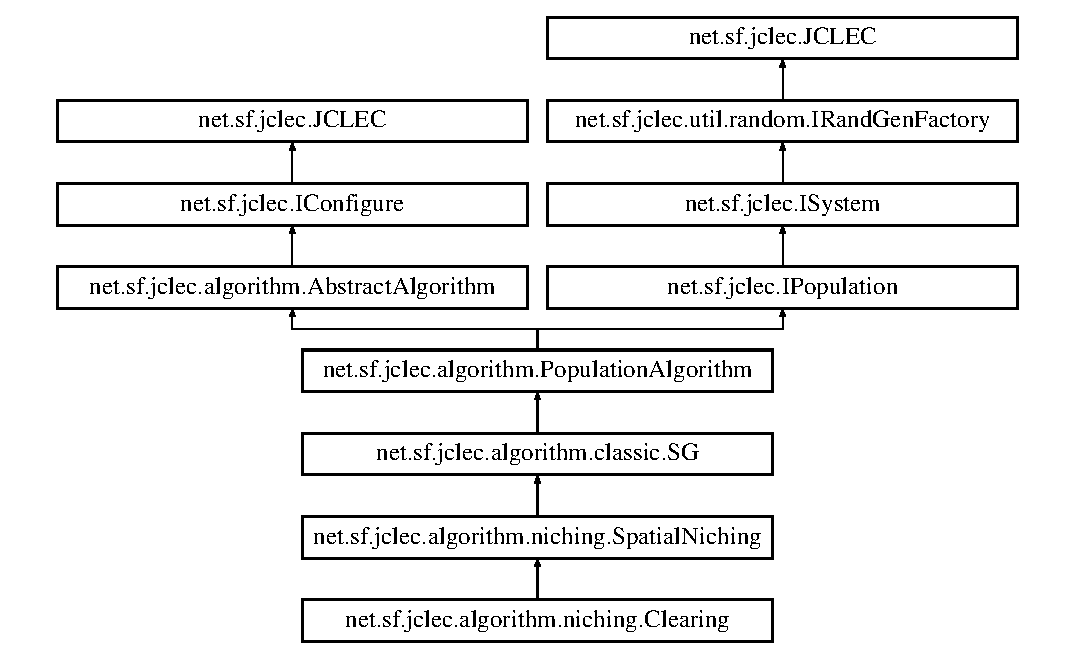
\includegraphics[height=8.000000cm]{classnet_1_1sf_1_1jclec_1_1algorithm_1_1niching_1_1_clearing}
\end{center}
\end{figure}
\subsection*{Public Member Functions}
\begin{DoxyCompactItemize}
\item 
\hyperlink{classnet_1_1sf_1_1jclec_1_1algorithm_1_1niching_1_1_clearing_a0e5ae5762d6d02fd9ad9d4bd5efa5ee1}{Clearing} ()
\item 
void \hyperlink{classnet_1_1sf_1_1jclec_1_1algorithm_1_1niching_1_1_clearing_a440e66f007b056d25542248a225492d2}{configure} (Configuration configuration)
\end{DoxyCompactItemize}
\subsection*{Protected Member Functions}
\begin{DoxyCompactItemize}
\item 
void \hyperlink{classnet_1_1sf_1_1jclec_1_1algorithm_1_1niching_1_1_clearing_a1df6eb4bbb13c57727a17612aa869210}{create\-Niches} ()
\end{DoxyCompactItemize}
\subsection*{Protected Attributes}
\begin{DoxyCompactItemize}
\item 
int \hyperlink{classnet_1_1sf_1_1jclec_1_1algorithm_1_1niching_1_1_clearing_a8702bf03f3e04215d9ea14fb792def04}{kappa}
\end{DoxyCompactItemize}


\subsection{Detailed Description}
Fitness clearing algorithm.

N\-O\-T\-E\-: This algorithm assumes that the optimal points to search are maximum points.

\begin{DoxyAuthor}{Author}
Sebastian Ventura 

Amelia Zafra 
\end{DoxyAuthor}


\subsection{Constructor \& Destructor Documentation}
\hypertarget{classnet_1_1sf_1_1jclec_1_1algorithm_1_1niching_1_1_clearing_a0e5ae5762d6d02fd9ad9d4bd5efa5ee1}{\index{net\-::sf\-::jclec\-::algorithm\-::niching\-::\-Clearing@{net\-::sf\-::jclec\-::algorithm\-::niching\-::\-Clearing}!Clearing@{Clearing}}
\index{Clearing@{Clearing}!net::sf::jclec::algorithm::niching::Clearing@{net\-::sf\-::jclec\-::algorithm\-::niching\-::\-Clearing}}
\subsubsection[{Clearing}]{\setlength{\rightskip}{0pt plus 5cm}net.\-sf.\-jclec.\-algorithm.\-niching.\-Clearing.\-Clearing (
\begin{DoxyParamCaption}
{}
\end{DoxyParamCaption}
)}}\label{classnet_1_1sf_1_1jclec_1_1algorithm_1_1niching_1_1_clearing_a0e5ae5762d6d02fd9ad9d4bd5efa5ee1}
Empty constructor 

\subsection{Member Function Documentation}
\hypertarget{classnet_1_1sf_1_1jclec_1_1algorithm_1_1niching_1_1_clearing_a440e66f007b056d25542248a225492d2}{\index{net\-::sf\-::jclec\-::algorithm\-::niching\-::\-Clearing@{net\-::sf\-::jclec\-::algorithm\-::niching\-::\-Clearing}!configure@{configure}}
\index{configure@{configure}!net::sf::jclec::algorithm::niching::Clearing@{net\-::sf\-::jclec\-::algorithm\-::niching\-::\-Clearing}}
\subsubsection[{configure}]{\setlength{\rightskip}{0pt plus 5cm}void net.\-sf.\-jclec.\-algorithm.\-niching.\-Clearing.\-configure (
\begin{DoxyParamCaption}
\item[{Configuration}]{configuration}
\end{DoxyParamCaption}
)}}\label{classnet_1_1sf_1_1jclec_1_1algorithm_1_1niching_1_1_clearing_a440e66f007b056d25542248a225492d2}
Configuration method.


\begin{DoxyParams}{Parameters}
{\em settings} & Configuration settings\\
\hline
\end{DoxyParams}


Configuration parameters for this algorithm are\-: 

Implements \hyperlink{interfacenet_1_1sf_1_1jclec_1_1_i_configure_add31a65a04d148c690a956fbbad6987c}{net.\-sf.\-jclec.\-I\-Configure}.

\hypertarget{classnet_1_1sf_1_1jclec_1_1algorithm_1_1niching_1_1_clearing_a1df6eb4bbb13c57727a17612aa869210}{\index{net\-::sf\-::jclec\-::algorithm\-::niching\-::\-Clearing@{net\-::sf\-::jclec\-::algorithm\-::niching\-::\-Clearing}!create\-Niches@{create\-Niches}}
\index{create\-Niches@{create\-Niches}!net::sf::jclec::algorithm::niching::Clearing@{net\-::sf\-::jclec\-::algorithm\-::niching\-::\-Clearing}}
\subsubsection[{create\-Niches}]{\setlength{\rightskip}{0pt plus 5cm}void net.\-sf.\-jclec.\-algorithm.\-niching.\-Clearing.\-create\-Niches (
\begin{DoxyParamCaption}
{}
\end{DoxyParamCaption}
)\hspace{0.3cm}{\ttfamily [protected]}, {\ttfamily [virtual]}}}\label{classnet_1_1sf_1_1jclec_1_1algorithm_1_1niching_1_1_clearing_a1df6eb4bbb13c57727a17612aa869210}
Assign fitness to all individuals in bset... 

Implements \hyperlink{classnet_1_1sf_1_1jclec_1_1algorithm_1_1niching_1_1_spatial_niching_aa0d6ea4c17a680c3beab861e17232af1}{net.\-sf.\-jclec.\-algorithm.\-niching.\-Spatial\-Niching}.



\subsection{Member Data Documentation}
\hypertarget{classnet_1_1sf_1_1jclec_1_1algorithm_1_1niching_1_1_clearing_a8702bf03f3e04215d9ea14fb792def04}{\index{net\-::sf\-::jclec\-::algorithm\-::niching\-::\-Clearing@{net\-::sf\-::jclec\-::algorithm\-::niching\-::\-Clearing}!kappa@{kappa}}
\index{kappa@{kappa}!net::sf::jclec::algorithm::niching::Clearing@{net\-::sf\-::jclec\-::algorithm\-::niching\-::\-Clearing}}
\subsubsection[{kappa}]{\setlength{\rightskip}{0pt plus 5cm}int net.\-sf.\-jclec.\-algorithm.\-niching.\-Clearing.\-kappa\hspace{0.3cm}{\ttfamily [protected]}}}\label{classnet_1_1sf_1_1jclec_1_1algorithm_1_1niching_1_1_clearing_a8702bf03f3e04215d9ea14fb792def04}
Number of individuals in each sub-\/population 

The documentation for this class was generated from the following file\-:\begin{DoxyCompactItemize}
\item 
src/main/java/net/sf/jclec/algorithm/niching/Clearing.\-java\end{DoxyCompactItemize}

\hypertarget{enumnet_1_1sf_1_1jclec_1_1util_1_1intset_1_1_closure}{\section{net.\-sf.\-jclec.\-util.\-intset.\-Closure Enum Reference}
\label{enumnet_1_1sf_1_1jclec_1_1util_1_1intset_1_1_closure}\index{net.\-sf.\-jclec.\-util.\-intset.\-Closure@{net.\-sf.\-jclec.\-util.\-intset.\-Closure}}
}
\subsection*{Public Attributes}
\begin{DoxyCompactItemize}
\item 
\hyperlink{enumnet_1_1sf_1_1jclec_1_1util_1_1intset_1_1_closure_afb6298f83e6ff0568ba2cd249c34017a}{Open\-Open}
\item 
\hyperlink{enumnet_1_1sf_1_1jclec_1_1util_1_1intset_1_1_closure_a305c17c3c719cc42552d28aa5ed04584}{Open\-Closed}
\item 
\hyperlink{enumnet_1_1sf_1_1jclec_1_1util_1_1intset_1_1_closure_a683ec132350559a9369150fd89356b7d}{Closed\-Open}
\item 
\hyperlink{enumnet_1_1sf_1_1jclec_1_1util_1_1intset_1_1_closure_a7f0eaa6fa09903548a1362c54c901023}{Closed\-Closed}
\end{DoxyCompactItemize}


\subsection{Detailed Description}
\hyperlink{classnet_1_1sf_1_1jclec_1_1util_1_1intset_1_1_interval}{Interval} closure.

\begin{DoxyAuthor}{Author}
Sebastian Ventura 
\end{DoxyAuthor}


\subsection{Member Data Documentation}
\hypertarget{enumnet_1_1sf_1_1jclec_1_1util_1_1intset_1_1_closure_a7f0eaa6fa09903548a1362c54c901023}{\index{net\-::sf\-::jclec\-::util\-::intset\-::\-Closure@{net\-::sf\-::jclec\-::util\-::intset\-::\-Closure}!Closed\-Closed@{Closed\-Closed}}
\index{Closed\-Closed@{Closed\-Closed}!net::sf::jclec::util::intset::Closure@{net\-::sf\-::jclec\-::util\-::intset\-::\-Closure}}
\subsubsection[{Closed\-Closed}]{\setlength{\rightskip}{0pt plus 5cm}net.\-sf.\-jclec.\-util.\-intset.\-Closure.\-Closed\-Closed}}\label{enumnet_1_1sf_1_1jclec_1_1util_1_1intset_1_1_closure_a7f0eaa6fa09903548a1362c54c901023}
\hyperlink{classnet_1_1sf_1_1jclec_1_1util_1_1intset_1_1_interval}{Interval} left and right closed \hypertarget{enumnet_1_1sf_1_1jclec_1_1util_1_1intset_1_1_closure_a683ec132350559a9369150fd89356b7d}{\index{net\-::sf\-::jclec\-::util\-::intset\-::\-Closure@{net\-::sf\-::jclec\-::util\-::intset\-::\-Closure}!Closed\-Open@{Closed\-Open}}
\index{Closed\-Open@{Closed\-Open}!net::sf::jclec::util::intset::Closure@{net\-::sf\-::jclec\-::util\-::intset\-::\-Closure}}
\subsubsection[{Closed\-Open}]{\setlength{\rightskip}{0pt plus 5cm}net.\-sf.\-jclec.\-util.\-intset.\-Closure.\-Closed\-Open}}\label{enumnet_1_1sf_1_1jclec_1_1util_1_1intset_1_1_closure_a683ec132350559a9369150fd89356b7d}
\hyperlink{classnet_1_1sf_1_1jclec_1_1util_1_1intset_1_1_interval}{Interval} left open and right closed \hypertarget{enumnet_1_1sf_1_1jclec_1_1util_1_1intset_1_1_closure_a305c17c3c719cc42552d28aa5ed04584}{\index{net\-::sf\-::jclec\-::util\-::intset\-::\-Closure@{net\-::sf\-::jclec\-::util\-::intset\-::\-Closure}!Open\-Closed@{Open\-Closed}}
\index{Open\-Closed@{Open\-Closed}!net::sf::jclec::util::intset::Closure@{net\-::sf\-::jclec\-::util\-::intset\-::\-Closure}}
\subsubsection[{Open\-Closed}]{\setlength{\rightskip}{0pt plus 5cm}net.\-sf.\-jclec.\-util.\-intset.\-Closure.\-Open\-Closed}}\label{enumnet_1_1sf_1_1jclec_1_1util_1_1intset_1_1_closure_a305c17c3c719cc42552d28aa5ed04584}
\hyperlink{classnet_1_1sf_1_1jclec_1_1util_1_1intset_1_1_interval}{Interval} left closed and right open \hypertarget{enumnet_1_1sf_1_1jclec_1_1util_1_1intset_1_1_closure_afb6298f83e6ff0568ba2cd249c34017a}{\index{net\-::sf\-::jclec\-::util\-::intset\-::\-Closure@{net\-::sf\-::jclec\-::util\-::intset\-::\-Closure}!Open\-Open@{Open\-Open}}
\index{Open\-Open@{Open\-Open}!net::sf::jclec::util::intset::Closure@{net\-::sf\-::jclec\-::util\-::intset\-::\-Closure}}
\subsubsection[{Open\-Open}]{\setlength{\rightskip}{0pt plus 5cm}net.\-sf.\-jclec.\-util.\-intset.\-Closure.\-Open\-Open}}\label{enumnet_1_1sf_1_1jclec_1_1util_1_1intset_1_1_closure_afb6298f83e6ff0568ba2cd249c34017a}
\hyperlink{classnet_1_1sf_1_1jclec_1_1util_1_1intset_1_1_interval}{Interval} left and right open 

The documentation for this enum was generated from the following file\-:\begin{DoxyCompactItemize}
\item 
src/main/java/net/sf/jclec/util/intset/Closure.\-java\end{DoxyCompactItemize}

\hypertarget{enumnet_1_1sf_1_1jclec_1_1util_1_1range_1_1_closure}{\section{net.\-sf.\-jclec.\-util.\-range.\-Closure Enum Reference}
\label{enumnet_1_1sf_1_1jclec_1_1util_1_1range_1_1_closure}\index{net.\-sf.\-jclec.\-util.\-range.\-Closure@{net.\-sf.\-jclec.\-util.\-range.\-Closure}}
}
\subsection*{Public Attributes}
\begin{DoxyCompactItemize}
\item 
\hyperlink{enumnet_1_1sf_1_1jclec_1_1util_1_1range_1_1_closure_a01aaf87015e4908454cd585add76fef1}{Open\-Open}
\item 
\hyperlink{enumnet_1_1sf_1_1jclec_1_1util_1_1range_1_1_closure_a900db0dc002751c7eeabc1502985bb93}{Open\-Closed}
\item 
\hyperlink{enumnet_1_1sf_1_1jclec_1_1util_1_1range_1_1_closure_aac450b1c65d6a7f6d4bc7c7378257c95}{Closed\-Open}
\item 
\hyperlink{enumnet_1_1sf_1_1jclec_1_1util_1_1range_1_1_closure_a7bc2bd20a327ebdf57009c19e28efade}{Closed\-Closed}
\end{DoxyCompactItemize}


\subsection{Detailed Description}
\hyperlink{classnet_1_1sf_1_1jclec_1_1util_1_1range_1_1_interval}{Interval} closure.

\begin{DoxyAuthor}{Author}
Sebastian Ventura 
\end{DoxyAuthor}


\subsection{Member Data Documentation}
\hypertarget{enumnet_1_1sf_1_1jclec_1_1util_1_1range_1_1_closure_a7bc2bd20a327ebdf57009c19e28efade}{\index{net\-::sf\-::jclec\-::util\-::range\-::\-Closure@{net\-::sf\-::jclec\-::util\-::range\-::\-Closure}!Closed\-Closed@{Closed\-Closed}}
\index{Closed\-Closed@{Closed\-Closed}!net::sf::jclec::util::range::Closure@{net\-::sf\-::jclec\-::util\-::range\-::\-Closure}}
\subsubsection[{Closed\-Closed}]{\setlength{\rightskip}{0pt plus 5cm}net.\-sf.\-jclec.\-util.\-range.\-Closure.\-Closed\-Closed}}\label{enumnet_1_1sf_1_1jclec_1_1util_1_1range_1_1_closure_a7bc2bd20a327ebdf57009c19e28efade}
\hyperlink{classnet_1_1sf_1_1jclec_1_1util_1_1range_1_1_interval}{Interval} left and right closed \hypertarget{enumnet_1_1sf_1_1jclec_1_1util_1_1range_1_1_closure_aac450b1c65d6a7f6d4bc7c7378257c95}{\index{net\-::sf\-::jclec\-::util\-::range\-::\-Closure@{net\-::sf\-::jclec\-::util\-::range\-::\-Closure}!Closed\-Open@{Closed\-Open}}
\index{Closed\-Open@{Closed\-Open}!net::sf::jclec::util::range::Closure@{net\-::sf\-::jclec\-::util\-::range\-::\-Closure}}
\subsubsection[{Closed\-Open}]{\setlength{\rightskip}{0pt plus 5cm}net.\-sf.\-jclec.\-util.\-range.\-Closure.\-Closed\-Open}}\label{enumnet_1_1sf_1_1jclec_1_1util_1_1range_1_1_closure_aac450b1c65d6a7f6d4bc7c7378257c95}
\hyperlink{classnet_1_1sf_1_1jclec_1_1util_1_1range_1_1_interval}{Interval} left open and right closed \hypertarget{enumnet_1_1sf_1_1jclec_1_1util_1_1range_1_1_closure_a900db0dc002751c7eeabc1502985bb93}{\index{net\-::sf\-::jclec\-::util\-::range\-::\-Closure@{net\-::sf\-::jclec\-::util\-::range\-::\-Closure}!Open\-Closed@{Open\-Closed}}
\index{Open\-Closed@{Open\-Closed}!net::sf::jclec::util::range::Closure@{net\-::sf\-::jclec\-::util\-::range\-::\-Closure}}
\subsubsection[{Open\-Closed}]{\setlength{\rightskip}{0pt plus 5cm}net.\-sf.\-jclec.\-util.\-range.\-Closure.\-Open\-Closed}}\label{enumnet_1_1sf_1_1jclec_1_1util_1_1range_1_1_closure_a900db0dc002751c7eeabc1502985bb93}
\hyperlink{classnet_1_1sf_1_1jclec_1_1util_1_1range_1_1_interval}{Interval} left closed and right open \hypertarget{enumnet_1_1sf_1_1jclec_1_1util_1_1range_1_1_closure_a01aaf87015e4908454cd585add76fef1}{\index{net\-::sf\-::jclec\-::util\-::range\-::\-Closure@{net\-::sf\-::jclec\-::util\-::range\-::\-Closure}!Open\-Open@{Open\-Open}}
\index{Open\-Open@{Open\-Open}!net::sf::jclec::util::range::Closure@{net\-::sf\-::jclec\-::util\-::range\-::\-Closure}}
\subsubsection[{Open\-Open}]{\setlength{\rightskip}{0pt plus 5cm}net.\-sf.\-jclec.\-util.\-range.\-Closure.\-Open\-Open}}\label{enumnet_1_1sf_1_1jclec_1_1util_1_1range_1_1_closure_a01aaf87015e4908454cd585add76fef1}
\hyperlink{classnet_1_1sf_1_1jclec_1_1util_1_1range_1_1_interval}{Interval} left and right open 

The documentation for this enum was generated from the following file\-:\begin{DoxyCompactItemize}
\item 
src/main/java/net/sf/jclec/util/range/Closure.\-java\end{DoxyCompactItemize}

\hypertarget{classnet_1_1sf_1_1jclec_1_1fitness_1_1_component_comparator}{\section{net.\-sf.\-jclec.\-fitness.\-Component\-Comparator Class Reference}
\label{classnet_1_1sf_1_1jclec_1_1fitness_1_1_component_comparator}\index{net.\-sf.\-jclec.\-fitness.\-Component\-Comparator@{net.\-sf.\-jclec.\-fitness.\-Component\-Comparator}}
}
Inheritance diagram for net.\-sf.\-jclec.\-fitness.\-Component\-Comparator\-:\begin{figure}[H]
\begin{center}
\leavevmode
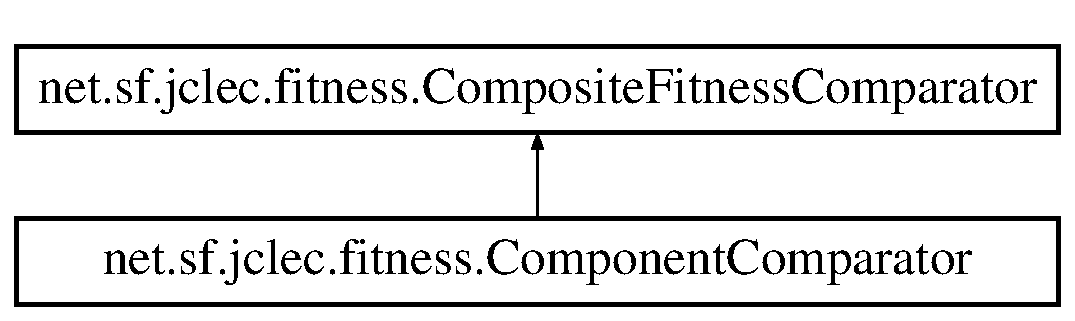
\includegraphics[height=2.000000cm]{classnet_1_1sf_1_1jclec_1_1fitness_1_1_component_comparator}
\end{center}
\end{figure}
\subsection*{Public Member Functions}
\begin{DoxyCompactItemize}
\item 
\hyperlink{classnet_1_1sf_1_1jclec_1_1fitness_1_1_component_comparator_a24bb0f31b4483a5402ab320e557f0949}{Component\-Comparator} ()
\item 
\hyperlink{classnet_1_1sf_1_1jclec_1_1fitness_1_1_component_comparator_a7f48852ccca7d46ce368fbd3f6803c5f}{Component\-Comparator} (Comparator$<$ \hyperlink{interfacenet_1_1sf_1_1jclec_1_1_i_fitness}{I\-Fitness} $>$\mbox{[}$\,$\mbox{]} \hyperlink{classnet_1_1sf_1_1jclec_1_1fitness_1_1_composite_fitness_comparator_a8448c857b752923973aba83432b52253}{component\-Comparators}, int \hyperlink{classnet_1_1sf_1_1jclec_1_1fitness_1_1_component_comparator_a7b4fea26c0f1dffe0b952992127bc4d7}{active\-Component\-Index})
\end{DoxyCompactItemize}
\subsection*{Protected Member Functions}
\begin{DoxyCompactItemize}
\item 
int \hyperlink{classnet_1_1sf_1_1jclec_1_1fitness_1_1_component_comparator_a0efa44541933fc99b581b7cd5f17aa3f}{compare} (\hyperlink{interfacenet_1_1sf_1_1jclec_1_1fitness_1_1_i_composite_fitness}{I\-Composite\-Fitness} cfitness0, \hyperlink{interfacenet_1_1sf_1_1jclec_1_1fitness_1_1_i_composite_fitness}{I\-Composite\-Fitness} cfitness1)
\end{DoxyCompactItemize}
\subsection*{Protected Attributes}
\begin{DoxyCompactItemize}
\item 
int \hyperlink{classnet_1_1sf_1_1jclec_1_1fitness_1_1_component_comparator_a7b4fea26c0f1dffe0b952992127bc4d7}{active\-Component\-Index}
\end{DoxyCompactItemize}


\subsection{Detailed Description}
Compare two \hyperlink{interfacenet_1_1sf_1_1jclec_1_1fitness_1_1_i_composite_fitness}{I\-Composite\-Fitness} objects according one of their components. The index of selected component is a user-\/defined parameter.

\begin{DoxyAuthor}{Author}
Sebastian Ventura 
\end{DoxyAuthor}


\subsection{Constructor \& Destructor Documentation}
\hypertarget{classnet_1_1sf_1_1jclec_1_1fitness_1_1_component_comparator_a24bb0f31b4483a5402ab320e557f0949}{\index{net\-::sf\-::jclec\-::fitness\-::\-Component\-Comparator@{net\-::sf\-::jclec\-::fitness\-::\-Component\-Comparator}!Component\-Comparator@{Component\-Comparator}}
\index{Component\-Comparator@{Component\-Comparator}!net::sf::jclec::fitness::ComponentComparator@{net\-::sf\-::jclec\-::fitness\-::\-Component\-Comparator}}
\subsubsection[{Component\-Comparator}]{\setlength{\rightskip}{0pt plus 5cm}net.\-sf.\-jclec.\-fitness.\-Component\-Comparator.\-Component\-Comparator (
\begin{DoxyParamCaption}
{}
\end{DoxyParamCaption}
)}}\label{classnet_1_1sf_1_1jclec_1_1fitness_1_1_component_comparator_a24bb0f31b4483a5402ab320e557f0949}
Empty constructor \hypertarget{classnet_1_1sf_1_1jclec_1_1fitness_1_1_component_comparator_a7f48852ccca7d46ce368fbd3f6803c5f}{\index{net\-::sf\-::jclec\-::fitness\-::\-Component\-Comparator@{net\-::sf\-::jclec\-::fitness\-::\-Component\-Comparator}!Component\-Comparator@{Component\-Comparator}}
\index{Component\-Comparator@{Component\-Comparator}!net::sf::jclec::fitness::ComponentComparator@{net\-::sf\-::jclec\-::fitness\-::\-Component\-Comparator}}
\subsubsection[{Component\-Comparator}]{\setlength{\rightskip}{0pt plus 5cm}net.\-sf.\-jclec.\-fitness.\-Component\-Comparator.\-Component\-Comparator (
\begin{DoxyParamCaption}
\item[{Comparator$<$ {\bf I\-Fitness} $>$\mbox{[}$\,$\mbox{]}}]{component\-Comparators, }
\item[{int}]{active\-Component\-Index}
\end{DoxyParamCaption}
)}}\label{classnet_1_1sf_1_1jclec_1_1fitness_1_1_component_comparator_a7f48852ccca7d46ce368fbd3f6803c5f}
Constructor that sets component comparators and active component index. 

\subsection{Member Function Documentation}
\hypertarget{classnet_1_1sf_1_1jclec_1_1fitness_1_1_component_comparator_a0efa44541933fc99b581b7cd5f17aa3f}{\index{net\-::sf\-::jclec\-::fitness\-::\-Component\-Comparator@{net\-::sf\-::jclec\-::fitness\-::\-Component\-Comparator}!compare@{compare}}
\index{compare@{compare}!net::sf::jclec::fitness::ComponentComparator@{net\-::sf\-::jclec\-::fitness\-::\-Component\-Comparator}}
\subsubsection[{compare}]{\setlength{\rightskip}{0pt plus 5cm}int net.\-sf.\-jclec.\-fitness.\-Component\-Comparator.\-compare (
\begin{DoxyParamCaption}
\item[{{\bf I\-Composite\-Fitness}}]{cfitness0, }
\item[{{\bf I\-Composite\-Fitness}}]{cfitness1}
\end{DoxyParamCaption}
)\hspace{0.3cm}{\ttfamily [protected]}, {\ttfamily [virtual]}}}\label{classnet_1_1sf_1_1jclec_1_1fitness_1_1_component_comparator_a0efa44541933fc99b581b7cd5f17aa3f}
Compare two composite fitnesses. 

Implements \hyperlink{classnet_1_1sf_1_1jclec_1_1fitness_1_1_composite_fitness_comparator_a6c060cd511a694dc0953e42ab05a4419}{net.\-sf.\-jclec.\-fitness.\-Composite\-Fitness\-Comparator}.



\subsection{Member Data Documentation}
\hypertarget{classnet_1_1sf_1_1jclec_1_1fitness_1_1_component_comparator_a7b4fea26c0f1dffe0b952992127bc4d7}{\index{net\-::sf\-::jclec\-::fitness\-::\-Component\-Comparator@{net\-::sf\-::jclec\-::fitness\-::\-Component\-Comparator}!active\-Component\-Index@{active\-Component\-Index}}
\index{active\-Component\-Index@{active\-Component\-Index}!net::sf::jclec::fitness::ComponentComparator@{net\-::sf\-::jclec\-::fitness\-::\-Component\-Comparator}}
\subsubsection[{active\-Component\-Index}]{\setlength{\rightskip}{0pt plus 5cm}int net.\-sf.\-jclec.\-fitness.\-Component\-Comparator.\-active\-Component\-Index\hspace{0.3cm}{\ttfamily [protected]}}}\label{classnet_1_1sf_1_1jclec_1_1fitness_1_1_component_comparator_a7b4fea26c0f1dffe0b952992127bc4d7}
Index of component that will be compared 

The documentation for this class was generated from the following file\-:\begin{DoxyCompactItemize}
\item 
src/main/java/net/sf/jclec/fitness/Component\-Comparator.\-java\end{DoxyCompactItemize}

\hypertarget{classnet_1_1sf_1_1jclec_1_1fitness_1_1_composite_fitness}{\section{net.\-sf.\-jclec.\-fitness.\-Composite\-Fitness Class Reference}
\label{classnet_1_1sf_1_1jclec_1_1fitness_1_1_composite_fitness}\index{net.\-sf.\-jclec.\-fitness.\-Composite\-Fitness@{net.\-sf.\-jclec.\-fitness.\-Composite\-Fitness}}
}
Inheritance diagram for net.\-sf.\-jclec.\-fitness.\-Composite\-Fitness\-:\begin{figure}[H]
\begin{center}
\leavevmode
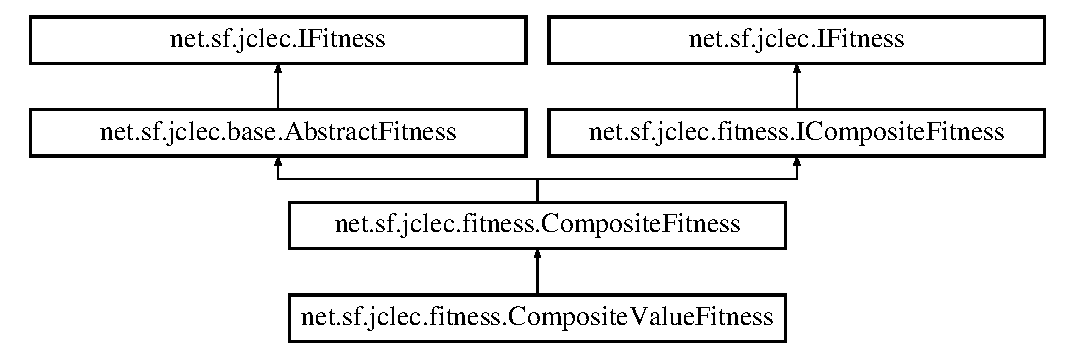
\includegraphics[height=5.000000cm]{classnet_1_1sf_1_1jclec_1_1fitness_1_1_composite_fitness}
\end{center}
\end{figure}
\subsection*{Public Member Functions}
\begin{DoxyCompactItemize}
\item 
\hyperlink{classnet_1_1sf_1_1jclec_1_1fitness_1_1_composite_fitness_a50c01e28a561e33a9dc101bd0d73f256}{Composite\-Fitness} ()
\item 
\hyperlink{classnet_1_1sf_1_1jclec_1_1fitness_1_1_composite_fitness_a64993a2474f07b180233c50bc2c69855}{Composite\-Fitness} (\hyperlink{interfacenet_1_1sf_1_1jclec_1_1fitness_1_1_i_simple_fitness}{I\-Simple\-Fitness}\mbox{[}$\,$\mbox{]} \hyperlink{classnet_1_1sf_1_1jclec_1_1fitness_1_1_composite_fitness_a07576591ce53292c41a9283d0baed349}{components})
\item 
\hyperlink{interfacenet_1_1sf_1_1jclec_1_1fitness_1_1_i_simple_fitness}{I\-Simple\-Fitness}\mbox{[}$\,$\mbox{]} \hyperlink{classnet_1_1sf_1_1jclec_1_1fitness_1_1_composite_fitness_aedda6ed56ded03d23302dc2af74acbcf}{get\-Components} ()
\item 
void \hyperlink{classnet_1_1sf_1_1jclec_1_1fitness_1_1_composite_fitness_a844b1290850a2af85a2f26a26ea569ea}{set\-Components} (\hyperlink{interfacenet_1_1sf_1_1jclec_1_1fitness_1_1_i_simple_fitness}{I\-Simple\-Fitness}\mbox{[}$\,$\mbox{]} \hyperlink{classnet_1_1sf_1_1jclec_1_1fitness_1_1_composite_fitness_a07576591ce53292c41a9283d0baed349}{components})
\item 
\hyperlink{interfacenet_1_1sf_1_1jclec_1_1fitness_1_1_i_simple_fitness}{I\-Simple\-Fitness} \hyperlink{classnet_1_1sf_1_1jclec_1_1fitness_1_1_composite_fitness_a91dfbecf11e3687bb1c475d8172dac65}{get\-Component} (int cidx)
\item 
void \hyperlink{classnet_1_1sf_1_1jclec_1_1fitness_1_1_composite_fitness_a15d0e15f3df82448ccc3d19945eeecde}{set\-Component} (int cidx, \hyperlink{interfacenet_1_1sf_1_1jclec_1_1fitness_1_1_i_simple_fitness}{I\-Simple\-Fitness} cval)
\item 
\hyperlink{interfacenet_1_1sf_1_1jclec_1_1_i_fitness}{I\-Fitness} \hyperlink{classnet_1_1sf_1_1jclec_1_1fitness_1_1_composite_fitness_add4d3a372842bde2a49fad94e03653c1}{copy} ()
\item 
int \hyperlink{classnet_1_1sf_1_1jclec_1_1fitness_1_1_composite_fitness_a186f49971ffbc28a891eb7756349faa8}{hash\-Code} ()
\item 
boolean \hyperlink{classnet_1_1sf_1_1jclec_1_1fitness_1_1_composite_fitness_a5af34e8b30c934faf50657e53fbc61ad}{equals} (Object oth)
\item 
String \hyperlink{classnet_1_1sf_1_1jclec_1_1fitness_1_1_composite_fitness_a5a6325fe5e88650700181ef92d995507}{to\-String} ()
\end{DoxyCompactItemize}
\subsection*{Protected Attributes}
\begin{DoxyCompactItemize}
\item 
\hyperlink{interfacenet_1_1sf_1_1jclec_1_1fitness_1_1_i_simple_fitness}{I\-Simple\-Fitness}\mbox{[}$\,$\mbox{]} \hyperlink{classnet_1_1sf_1_1jclec_1_1fitness_1_1_composite_fitness_a07576591ce53292c41a9283d0baed349}{components}
\end{DoxyCompactItemize}


\subsection{Detailed Description}
Composite fitness.

\begin{DoxyAuthor}{Author}
Sebastian Ventura 
\end{DoxyAuthor}


\subsection{Constructor \& Destructor Documentation}
\hypertarget{classnet_1_1sf_1_1jclec_1_1fitness_1_1_composite_fitness_a50c01e28a561e33a9dc101bd0d73f256}{\index{net\-::sf\-::jclec\-::fitness\-::\-Composite\-Fitness@{net\-::sf\-::jclec\-::fitness\-::\-Composite\-Fitness}!Composite\-Fitness@{Composite\-Fitness}}
\index{Composite\-Fitness@{Composite\-Fitness}!net::sf::jclec::fitness::CompositeFitness@{net\-::sf\-::jclec\-::fitness\-::\-Composite\-Fitness}}
\subsubsection[{Composite\-Fitness}]{\setlength{\rightskip}{0pt plus 5cm}net.\-sf.\-jclec.\-fitness.\-Composite\-Fitness.\-Composite\-Fitness (
\begin{DoxyParamCaption}
{}
\end{DoxyParamCaption}
)}}\label{classnet_1_1sf_1_1jclec_1_1fitness_1_1_composite_fitness_a50c01e28a561e33a9dc101bd0d73f256}
Empty constructor \hypertarget{classnet_1_1sf_1_1jclec_1_1fitness_1_1_composite_fitness_a64993a2474f07b180233c50bc2c69855}{\index{net\-::sf\-::jclec\-::fitness\-::\-Composite\-Fitness@{net\-::sf\-::jclec\-::fitness\-::\-Composite\-Fitness}!Composite\-Fitness@{Composite\-Fitness}}
\index{Composite\-Fitness@{Composite\-Fitness}!net::sf::jclec::fitness::CompositeFitness@{net\-::sf\-::jclec\-::fitness\-::\-Composite\-Fitness}}
\subsubsection[{Composite\-Fitness}]{\setlength{\rightskip}{0pt plus 5cm}net.\-sf.\-jclec.\-fitness.\-Composite\-Fitness.\-Composite\-Fitness (
\begin{DoxyParamCaption}
\item[{{\bf I\-Simple\-Fitness}\mbox{[}$\,$\mbox{]}}]{components}
\end{DoxyParamCaption}
)}}\label{classnet_1_1sf_1_1jclec_1_1fitness_1_1_composite_fitness_a64993a2474f07b180233c50bc2c69855}
Default constructor. Sets fitness components


\begin{DoxyParams}{Parameters}
{\em components} & Fitness components \\
\hline
\end{DoxyParams}


\subsection{Member Function Documentation}
\hypertarget{classnet_1_1sf_1_1jclec_1_1fitness_1_1_composite_fitness_add4d3a372842bde2a49fad94e03653c1}{\index{net\-::sf\-::jclec\-::fitness\-::\-Composite\-Fitness@{net\-::sf\-::jclec\-::fitness\-::\-Composite\-Fitness}!copy@{copy}}
\index{copy@{copy}!net::sf::jclec::fitness::CompositeFitness@{net\-::sf\-::jclec\-::fitness\-::\-Composite\-Fitness}}
\subsubsection[{copy}]{\setlength{\rightskip}{0pt plus 5cm}{\bf I\-Fitness} net.\-sf.\-jclec.\-fitness.\-Composite\-Fitness.\-copy (
\begin{DoxyParamCaption}
{}
\end{DoxyParamCaption}
)}}\label{classnet_1_1sf_1_1jclec_1_1fitness_1_1_composite_fitness_add4d3a372842bde2a49fad94e03653c1}
Copy method.

\begin{DoxyReturn}{Returns}
a copy of this fitness.
\end{DoxyReturn}
 

Implements \hyperlink{interfacenet_1_1sf_1_1jclec_1_1_i_fitness_ae93ff10d671a76d5712835de329178bc}{net.\-sf.\-jclec.\-I\-Fitness}.

\hypertarget{classnet_1_1sf_1_1jclec_1_1fitness_1_1_composite_fitness_a5af34e8b30c934faf50657e53fbc61ad}{\index{net\-::sf\-::jclec\-::fitness\-::\-Composite\-Fitness@{net\-::sf\-::jclec\-::fitness\-::\-Composite\-Fitness}!equals@{equals}}
\index{equals@{equals}!net::sf::jclec::fitness::CompositeFitness@{net\-::sf\-::jclec\-::fitness\-::\-Composite\-Fitness}}
\subsubsection[{equals}]{\setlength{\rightskip}{0pt plus 5cm}boolean net.\-sf.\-jclec.\-fitness.\-Composite\-Fitness.\-equals (
\begin{DoxyParamCaption}
\item[{Object}]{oth}
\end{DoxyParamCaption}
)}}\label{classnet_1_1sf_1_1jclec_1_1fitness_1_1_composite_fitness_a5af34e8b30c934faf50657e53fbc61ad}
\hypertarget{classnet_1_1sf_1_1jclec_1_1fitness_1_1_composite_fitness_a91dfbecf11e3687bb1c475d8172dac65}{\index{net\-::sf\-::jclec\-::fitness\-::\-Composite\-Fitness@{net\-::sf\-::jclec\-::fitness\-::\-Composite\-Fitness}!get\-Component@{get\-Component}}
\index{get\-Component@{get\-Component}!net::sf::jclec::fitness::CompositeFitness@{net\-::sf\-::jclec\-::fitness\-::\-Composite\-Fitness}}
\subsubsection[{get\-Component}]{\setlength{\rightskip}{0pt plus 5cm}{\bf I\-Simple\-Fitness} net.\-sf.\-jclec.\-fitness.\-Composite\-Fitness.\-get\-Component (
\begin{DoxyParamCaption}
\item[{int}]{cidx}
\end{DoxyParamCaption}
)}}\label{classnet_1_1sf_1_1jclec_1_1fitness_1_1_composite_fitness_a91dfbecf11e3687bb1c475d8172dac65}
Returns a fitness component.


\begin{DoxyParams}{Parameters}
{\em cidx} & Index of desired index.\\
\hline
\end{DoxyParams}
\begin{DoxyReturn}{Returns}
cidx-\/throws fitness component 
\end{DoxyReturn}


Implements \hyperlink{interfacenet_1_1sf_1_1jclec_1_1fitness_1_1_i_composite_fitness_a7a90bfd8df1d05ed16153e647a9f1d99}{net.\-sf.\-jclec.\-fitness.\-I\-Composite\-Fitness}.

\hypertarget{classnet_1_1sf_1_1jclec_1_1fitness_1_1_composite_fitness_aedda6ed56ded03d23302dc2af74acbcf}{\index{net\-::sf\-::jclec\-::fitness\-::\-Composite\-Fitness@{net\-::sf\-::jclec\-::fitness\-::\-Composite\-Fitness}!get\-Components@{get\-Components}}
\index{get\-Components@{get\-Components}!net::sf::jclec::fitness::CompositeFitness@{net\-::sf\-::jclec\-::fitness\-::\-Composite\-Fitness}}
\subsubsection[{get\-Components}]{\setlength{\rightskip}{0pt plus 5cm}{\bf I\-Simple\-Fitness} \mbox{[}$\,$\mbox{]} net.\-sf.\-jclec.\-fitness.\-Composite\-Fitness.\-get\-Components (
\begin{DoxyParamCaption}
{}
\end{DoxyParamCaption}
)}}\label{classnet_1_1sf_1_1jclec_1_1fitness_1_1_composite_fitness_aedda6ed56ded03d23302dc2af74acbcf}
\begin{DoxyReturn}{Returns}
This fitness components 
\end{DoxyReturn}


Implements \hyperlink{interfacenet_1_1sf_1_1jclec_1_1fitness_1_1_i_composite_fitness_aa5028f84af2e42e98747990a1818a3f5}{net.\-sf.\-jclec.\-fitness.\-I\-Composite\-Fitness}.

\hypertarget{classnet_1_1sf_1_1jclec_1_1fitness_1_1_composite_fitness_a186f49971ffbc28a891eb7756349faa8}{\index{net\-::sf\-::jclec\-::fitness\-::\-Composite\-Fitness@{net\-::sf\-::jclec\-::fitness\-::\-Composite\-Fitness}!hash\-Code@{hash\-Code}}
\index{hash\-Code@{hash\-Code}!net::sf::jclec::fitness::CompositeFitness@{net\-::sf\-::jclec\-::fitness\-::\-Composite\-Fitness}}
\subsubsection[{hash\-Code}]{\setlength{\rightskip}{0pt plus 5cm}int net.\-sf.\-jclec.\-fitness.\-Composite\-Fitness.\-hash\-Code (
\begin{DoxyParamCaption}
{}
\end{DoxyParamCaption}
)}}\label{classnet_1_1sf_1_1jclec_1_1fitness_1_1_composite_fitness_a186f49971ffbc28a891eb7756349faa8}
\hypertarget{classnet_1_1sf_1_1jclec_1_1fitness_1_1_composite_fitness_a15d0e15f3df82448ccc3d19945eeecde}{\index{net\-::sf\-::jclec\-::fitness\-::\-Composite\-Fitness@{net\-::sf\-::jclec\-::fitness\-::\-Composite\-Fitness}!set\-Component@{set\-Component}}
\index{set\-Component@{set\-Component}!net::sf::jclec::fitness::CompositeFitness@{net\-::sf\-::jclec\-::fitness\-::\-Composite\-Fitness}}
\subsubsection[{set\-Component}]{\setlength{\rightskip}{0pt plus 5cm}void net.\-sf.\-jclec.\-fitness.\-Composite\-Fitness.\-set\-Component (
\begin{DoxyParamCaption}
\item[{int}]{cidx, }
\item[{{\bf I\-Simple\-Fitness}}]{cval}
\end{DoxyParamCaption}
)}}\label{classnet_1_1sf_1_1jclec_1_1fitness_1_1_composite_fitness_a15d0e15f3df82448ccc3d19945eeecde}
Sets a fitness component.


\begin{DoxyParams}{Parameters}
{\em cidx} & Index of desired component \\
\hline
{\em cval} & Desired component value. \\
\hline
\end{DoxyParams}


Implements \hyperlink{interfacenet_1_1sf_1_1jclec_1_1fitness_1_1_i_composite_fitness_a681e21343657e866148af83709ae85b8}{net.\-sf.\-jclec.\-fitness.\-I\-Composite\-Fitness}.

\hypertarget{classnet_1_1sf_1_1jclec_1_1fitness_1_1_composite_fitness_a844b1290850a2af85a2f26a26ea569ea}{\index{net\-::sf\-::jclec\-::fitness\-::\-Composite\-Fitness@{net\-::sf\-::jclec\-::fitness\-::\-Composite\-Fitness}!set\-Components@{set\-Components}}
\index{set\-Components@{set\-Components}!net::sf::jclec::fitness::CompositeFitness@{net\-::sf\-::jclec\-::fitness\-::\-Composite\-Fitness}}
\subsubsection[{set\-Components}]{\setlength{\rightskip}{0pt plus 5cm}void net.\-sf.\-jclec.\-fitness.\-Composite\-Fitness.\-set\-Components (
\begin{DoxyParamCaption}
\item[{{\bf I\-Simple\-Fitness}\mbox{[}$\,$\mbox{]}}]{components}
\end{DoxyParamCaption}
)}}\label{classnet_1_1sf_1_1jclec_1_1fitness_1_1_composite_fitness_a844b1290850a2af85a2f26a26ea569ea}
Sets this fitness components.


\begin{DoxyParams}{Parameters}
{\em components} & New fitness components. \\
\hline
\end{DoxyParams}


Implements \hyperlink{interfacenet_1_1sf_1_1jclec_1_1fitness_1_1_i_composite_fitness_a4e0df445defe2719606810e62be2ef26}{net.\-sf.\-jclec.\-fitness.\-I\-Composite\-Fitness}.

\hypertarget{classnet_1_1sf_1_1jclec_1_1fitness_1_1_composite_fitness_a5a6325fe5e88650700181ef92d995507}{\index{net\-::sf\-::jclec\-::fitness\-::\-Composite\-Fitness@{net\-::sf\-::jclec\-::fitness\-::\-Composite\-Fitness}!to\-String@{to\-String}}
\index{to\-String@{to\-String}!net::sf::jclec::fitness::CompositeFitness@{net\-::sf\-::jclec\-::fitness\-::\-Composite\-Fitness}}
\subsubsection[{to\-String}]{\setlength{\rightskip}{0pt plus 5cm}String net.\-sf.\-jclec.\-fitness.\-Composite\-Fitness.\-to\-String (
\begin{DoxyParamCaption}
{}
\end{DoxyParamCaption}
)}}\label{classnet_1_1sf_1_1jclec_1_1fitness_1_1_composite_fitness_a5a6325fe5e88650700181ef92d995507}


\subsection{Member Data Documentation}
\hypertarget{classnet_1_1sf_1_1jclec_1_1fitness_1_1_composite_fitness_a07576591ce53292c41a9283d0baed349}{\index{net\-::sf\-::jclec\-::fitness\-::\-Composite\-Fitness@{net\-::sf\-::jclec\-::fitness\-::\-Composite\-Fitness}!components@{components}}
\index{components@{components}!net::sf::jclec::fitness::CompositeFitness@{net\-::sf\-::jclec\-::fitness\-::\-Composite\-Fitness}}
\subsubsection[{components}]{\setlength{\rightskip}{0pt plus 5cm}{\bf I\-Simple\-Fitness} \mbox{[}$\,$\mbox{]} net.\-sf.\-jclec.\-fitness.\-Composite\-Fitness.\-components\hspace{0.3cm}{\ttfamily [protected]}}}\label{classnet_1_1sf_1_1jclec_1_1fitness_1_1_composite_fitness_a07576591ce53292c41a9283d0baed349}
Fitness components 

The documentation for this class was generated from the following file\-:\begin{DoxyCompactItemize}
\item 
src/main/java/net/sf/jclec/fitness/Composite\-Fitness.\-java\end{DoxyCompactItemize}

\hypertarget{classnet_1_1sf_1_1jclec_1_1fitness_1_1_composite_fitness_comparator}{\section{net.\-sf.\-jclec.\-fitness.\-Composite\-Fitness\-Comparator Class Reference}
\label{classnet_1_1sf_1_1jclec_1_1fitness_1_1_composite_fitness_comparator}\index{net.\-sf.\-jclec.\-fitness.\-Composite\-Fitness\-Comparator@{net.\-sf.\-jclec.\-fitness.\-Composite\-Fitness\-Comparator}}
}
Inheritance diagram for net.\-sf.\-jclec.\-fitness.\-Composite\-Fitness\-Comparator\-:\begin{figure}[H]
\begin{center}
\leavevmode
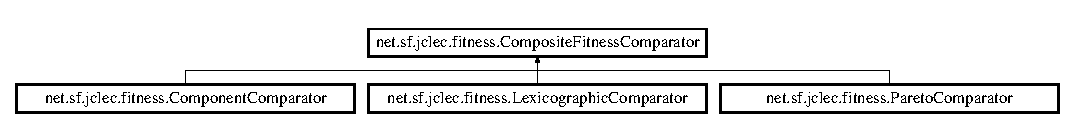
\includegraphics[height=1.287356cm]{classnet_1_1sf_1_1jclec_1_1fitness_1_1_composite_fitness_comparator}
\end{center}
\end{figure}
\subsection*{Public Member Functions}
\begin{DoxyCompactItemize}
\item 
\hyperlink{classnet_1_1sf_1_1jclec_1_1fitness_1_1_composite_fitness_comparator_a06415294cd3b7e0a3c55106c386e24dc}{Composite\-Fitness\-Comparator} ()
\item 
\hyperlink{classnet_1_1sf_1_1jclec_1_1fitness_1_1_composite_fitness_comparator_ac2a8fda5aba7a8d4c311c799e04a5399}{Composite\-Fitness\-Comparator} (Comparator$<$ \hyperlink{interfacenet_1_1sf_1_1jclec_1_1_i_fitness}{I\-Fitness} $>$\mbox{[}$\,$\mbox{]} \hyperlink{classnet_1_1sf_1_1jclec_1_1fitness_1_1_composite_fitness_comparator_a8448c857b752923973aba83432b52253}{component\-Comparators})
\item 
Comparator$<$ \hyperlink{interfacenet_1_1sf_1_1jclec_1_1_i_fitness}{I\-Fitness} $>$\mbox{[}$\,$\mbox{]} \hyperlink{classnet_1_1sf_1_1jclec_1_1fitness_1_1_composite_fitness_comparator_adc84063f52e886c2ae95bc610eac7b43}{get\-Component\-Comparators} ()
\item 
void \hyperlink{classnet_1_1sf_1_1jclec_1_1fitness_1_1_composite_fitness_comparator_ab8078b469b029ce1e96a596e0c90b57d}{set\-Component\-Comparators} (Comparator$<$ \hyperlink{interfacenet_1_1sf_1_1jclec_1_1_i_fitness}{I\-Fitness} $>$\mbox{[}$\,$\mbox{]} \hyperlink{classnet_1_1sf_1_1jclec_1_1fitness_1_1_composite_fitness_comparator_a8448c857b752923973aba83432b52253}{component\-Comparators})
\end{DoxyCompactItemize}
\subsection*{Protected Member Functions}
\begin{DoxyCompactItemize}
\item 
abstract int \hyperlink{classnet_1_1sf_1_1jclec_1_1fitness_1_1_composite_fitness_comparator_a6c060cd511a694dc0953e42ab05a4419}{compare} (\hyperlink{interfacenet_1_1sf_1_1jclec_1_1fitness_1_1_i_composite_fitness}{I\-Composite\-Fitness} cfitness0, \hyperlink{interfacenet_1_1sf_1_1jclec_1_1fitness_1_1_i_composite_fitness}{I\-Composite\-Fitness} cfitness1)
\end{DoxyCompactItemize}
\subsection*{Protected Attributes}
\begin{DoxyCompactItemize}
\item 
Comparator$<$ \hyperlink{interfacenet_1_1sf_1_1jclec_1_1_i_fitness}{I\-Fitness} $>$\mbox{[}$\,$\mbox{]} \hyperlink{classnet_1_1sf_1_1jclec_1_1fitness_1_1_composite_fitness_comparator_a8448c857b752923973aba83432b52253}{component\-Comparators}
\end{DoxyCompactItemize}


\subsection{Detailed Description}
Compare two \hyperlink{interfacenet_1_1sf_1_1jclec_1_1fitness_1_1_i_composite_fitness}{I\-Composite\-Fitness} objects.

\begin{DoxyAuthor}{Author}
Sebastian Ventura 
\end{DoxyAuthor}


\subsection{Constructor \& Destructor Documentation}
\hypertarget{classnet_1_1sf_1_1jclec_1_1fitness_1_1_composite_fitness_comparator_a06415294cd3b7e0a3c55106c386e24dc}{\index{net\-::sf\-::jclec\-::fitness\-::\-Composite\-Fitness\-Comparator@{net\-::sf\-::jclec\-::fitness\-::\-Composite\-Fitness\-Comparator}!Composite\-Fitness\-Comparator@{Composite\-Fitness\-Comparator}}
\index{Composite\-Fitness\-Comparator@{Composite\-Fitness\-Comparator}!net::sf::jclec::fitness::CompositeFitnessComparator@{net\-::sf\-::jclec\-::fitness\-::\-Composite\-Fitness\-Comparator}}
\subsubsection[{Composite\-Fitness\-Comparator}]{\setlength{\rightskip}{0pt plus 5cm}net.\-sf.\-jclec.\-fitness.\-Composite\-Fitness\-Comparator.\-Composite\-Fitness\-Comparator (
\begin{DoxyParamCaption}
{}
\end{DoxyParamCaption}
)}}\label{classnet_1_1sf_1_1jclec_1_1fitness_1_1_composite_fitness_comparator_a06415294cd3b7e0a3c55106c386e24dc}
Empty constructor. \hypertarget{classnet_1_1sf_1_1jclec_1_1fitness_1_1_composite_fitness_comparator_ac2a8fda5aba7a8d4c311c799e04a5399}{\index{net\-::sf\-::jclec\-::fitness\-::\-Composite\-Fitness\-Comparator@{net\-::sf\-::jclec\-::fitness\-::\-Composite\-Fitness\-Comparator}!Composite\-Fitness\-Comparator@{Composite\-Fitness\-Comparator}}
\index{Composite\-Fitness\-Comparator@{Composite\-Fitness\-Comparator}!net::sf::jclec::fitness::CompositeFitnessComparator@{net\-::sf\-::jclec\-::fitness\-::\-Composite\-Fitness\-Comparator}}
\subsubsection[{Composite\-Fitness\-Comparator}]{\setlength{\rightskip}{0pt plus 5cm}net.\-sf.\-jclec.\-fitness.\-Composite\-Fitness\-Comparator.\-Composite\-Fitness\-Comparator (
\begin{DoxyParamCaption}
\item[{Comparator$<$ {\bf I\-Fitness} $>$\mbox{[}$\,$\mbox{]}}]{component\-Comparators}
\end{DoxyParamCaption}
)}}\label{classnet_1_1sf_1_1jclec_1_1fitness_1_1_composite_fitness_comparator_ac2a8fda5aba7a8d4c311c799e04a5399}
Constructor that set component fitness comparators.


\begin{DoxyParams}{Parameters}
{\em component\-Comparators} & Component fitness comparators \\
\hline
\end{DoxyParams}


\subsection{Member Function Documentation}
\hypertarget{classnet_1_1sf_1_1jclec_1_1fitness_1_1_composite_fitness_comparator_a6c060cd511a694dc0953e42ab05a4419}{\index{net\-::sf\-::jclec\-::fitness\-::\-Composite\-Fitness\-Comparator@{net\-::sf\-::jclec\-::fitness\-::\-Composite\-Fitness\-Comparator}!compare@{compare}}
\index{compare@{compare}!net::sf::jclec::fitness::CompositeFitnessComparator@{net\-::sf\-::jclec\-::fitness\-::\-Composite\-Fitness\-Comparator}}
\subsubsection[{compare}]{\setlength{\rightskip}{0pt plus 5cm}abstract int net.\-sf.\-jclec.\-fitness.\-Composite\-Fitness\-Comparator.\-compare (
\begin{DoxyParamCaption}
\item[{{\bf I\-Composite\-Fitness}}]{cfitness0, }
\item[{{\bf I\-Composite\-Fitness}}]{cfitness1}
\end{DoxyParamCaption}
)\hspace{0.3cm}{\ttfamily [protected]}, {\ttfamily [pure virtual]}}}\label{classnet_1_1sf_1_1jclec_1_1fitness_1_1_composite_fitness_comparator_a6c060cd511a694dc0953e42ab05a4419}
Compare two composite fitnesses. 

Implemented in \hyperlink{classnet_1_1sf_1_1jclec_1_1fitness_1_1_component_comparator_a0efa44541933fc99b581b7cd5f17aa3f}{net.\-sf.\-jclec.\-fitness.\-Component\-Comparator}, \hyperlink{classnet_1_1sf_1_1jclec_1_1fitness_1_1_lexicographic_comparator_ae157ca7826ebee623cce24f6eebdf99b}{net.\-sf.\-jclec.\-fitness.\-Lexicographic\-Comparator}, and \hyperlink{classnet_1_1sf_1_1jclec_1_1fitness_1_1_pareto_comparator_af38a1bbd5a0c5e5b633bb4da8ef8e2a2}{net.\-sf.\-jclec.\-fitness.\-Pareto\-Comparator}.

\hypertarget{classnet_1_1sf_1_1jclec_1_1fitness_1_1_composite_fitness_comparator_adc84063f52e886c2ae95bc610eac7b43}{\index{net\-::sf\-::jclec\-::fitness\-::\-Composite\-Fitness\-Comparator@{net\-::sf\-::jclec\-::fitness\-::\-Composite\-Fitness\-Comparator}!get\-Component\-Comparators@{get\-Component\-Comparators}}
\index{get\-Component\-Comparators@{get\-Component\-Comparators}!net::sf::jclec::fitness::CompositeFitnessComparator@{net\-::sf\-::jclec\-::fitness\-::\-Composite\-Fitness\-Comparator}}
\subsubsection[{get\-Component\-Comparators}]{\setlength{\rightskip}{0pt plus 5cm}Comparator$<${\bf I\-Fitness}$>$ \mbox{[}$\,$\mbox{]} net.\-sf.\-jclec.\-fitness.\-Composite\-Fitness\-Comparator.\-get\-Component\-Comparators (
\begin{DoxyParamCaption}
{}
\end{DoxyParamCaption}
)}}\label{classnet_1_1sf_1_1jclec_1_1fitness_1_1_composite_fitness_comparator_adc84063f52e886c2ae95bc610eac7b43}
Access to component fitness comparators

\begin{DoxyReturn}{Returns}
Component fitness comparators 
\end{DoxyReturn}
\hypertarget{classnet_1_1sf_1_1jclec_1_1fitness_1_1_composite_fitness_comparator_ab8078b469b029ce1e96a596e0c90b57d}{\index{net\-::sf\-::jclec\-::fitness\-::\-Composite\-Fitness\-Comparator@{net\-::sf\-::jclec\-::fitness\-::\-Composite\-Fitness\-Comparator}!set\-Component\-Comparators@{set\-Component\-Comparators}}
\index{set\-Component\-Comparators@{set\-Component\-Comparators}!net::sf::jclec::fitness::CompositeFitnessComparator@{net\-::sf\-::jclec\-::fitness\-::\-Composite\-Fitness\-Comparator}}
\subsubsection[{set\-Component\-Comparators}]{\setlength{\rightskip}{0pt plus 5cm}void net.\-sf.\-jclec.\-fitness.\-Composite\-Fitness\-Comparator.\-set\-Component\-Comparators (
\begin{DoxyParamCaption}
\item[{Comparator$<$ {\bf I\-Fitness} $>$\mbox{[}$\,$\mbox{]}}]{component\-Comparators}
\end{DoxyParamCaption}
)}}\label{classnet_1_1sf_1_1jclec_1_1fitness_1_1_composite_fitness_comparator_ab8078b469b029ce1e96a596e0c90b57d}
Set component fitness comparators.


\begin{DoxyParams}{Parameters}
{\em component\-Comparators} & Component fitness comparators \\
\hline
\end{DoxyParams}


\subsection{Member Data Documentation}
\hypertarget{classnet_1_1sf_1_1jclec_1_1fitness_1_1_composite_fitness_comparator_a8448c857b752923973aba83432b52253}{\index{net\-::sf\-::jclec\-::fitness\-::\-Composite\-Fitness\-Comparator@{net\-::sf\-::jclec\-::fitness\-::\-Composite\-Fitness\-Comparator}!component\-Comparators@{component\-Comparators}}
\index{component\-Comparators@{component\-Comparators}!net::sf::jclec::fitness::CompositeFitnessComparator@{net\-::sf\-::jclec\-::fitness\-::\-Composite\-Fitness\-Comparator}}
\subsubsection[{component\-Comparators}]{\setlength{\rightskip}{0pt plus 5cm}Comparator$<${\bf I\-Fitness}$>$ \mbox{[}$\,$\mbox{]} net.\-sf.\-jclec.\-fitness.\-Composite\-Fitness\-Comparator.\-component\-Comparators\hspace{0.3cm}{\ttfamily [protected]}}}\label{classnet_1_1sf_1_1jclec_1_1fitness_1_1_composite_fitness_comparator_a8448c857b752923973aba83432b52253}
Component fitness comparators 

The documentation for this class was generated from the following file\-:\begin{DoxyCompactItemize}
\item 
src/main/java/net/sf/jclec/fitness/Composite\-Fitness\-Comparator.\-java\end{DoxyCompactItemize}

\hypertarget{classnet_1_1sf_1_1jclec_1_1fitness_1_1_composite_value_fitness}{\section{net.\-sf.\-jclec.\-fitness.\-Composite\-Value\-Fitness Class Reference}
\label{classnet_1_1sf_1_1jclec_1_1fitness_1_1_composite_value_fitness}\index{net.\-sf.\-jclec.\-fitness.\-Composite\-Value\-Fitness@{net.\-sf.\-jclec.\-fitness.\-Composite\-Value\-Fitness}}
}
Inheritance diagram for net.\-sf.\-jclec.\-fitness.\-Composite\-Value\-Fitness\-:\begin{figure}[H]
\begin{center}
\leavevmode
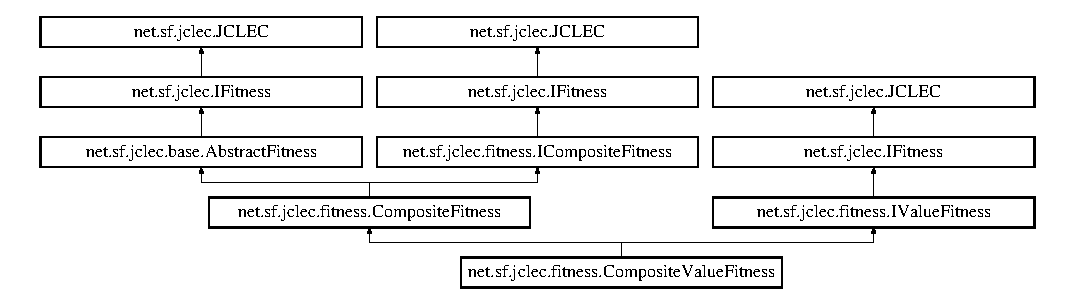
\includegraphics[height=3.631647cm]{classnet_1_1sf_1_1jclec_1_1fitness_1_1_composite_value_fitness}
\end{center}
\end{figure}
\subsection*{Public Member Functions}
\begin{DoxyCompactItemize}
\item 
\hyperlink{classnet_1_1sf_1_1jclec_1_1fitness_1_1_composite_value_fitness_a7886c2f50b76ad4433cf2ca7f4fc90b6}{Composite\-Value\-Fitness} ()
\item 
\hyperlink{classnet_1_1sf_1_1jclec_1_1fitness_1_1_composite_value_fitness_a30482c0efc4dbe8b0364bf9c5d79c0a4}{Composite\-Value\-Fitness} (\hyperlink{interfacenet_1_1sf_1_1jclec_1_1fitness_1_1_i_simple_fitness}{I\-Simple\-Fitness}\mbox{[}$\,$\mbox{]} \hyperlink{classnet_1_1sf_1_1jclec_1_1fitness_1_1_composite_fitness_a07576591ce53292c41a9283d0baed349}{components})
\item 
\hyperlink{classnet_1_1sf_1_1jclec_1_1fitness_1_1_composite_value_fitness_a5a712eea27ae7d02c46bd6b30ccf6049}{Composite\-Value\-Fitness} (\hyperlink{interfacenet_1_1sf_1_1jclec_1_1fitness_1_1_i_simple_fitness}{I\-Simple\-Fitness}\mbox{[}$\,$\mbox{]} \hyperlink{classnet_1_1sf_1_1jclec_1_1fitness_1_1_composite_fitness_a07576591ce53292c41a9283d0baed349}{components}, double \hyperlink{classnet_1_1sf_1_1jclec_1_1fitness_1_1_composite_value_fitness_a5b325c383bcdfd09c8277bafe55401bf}{value})
\item 
final double \hyperlink{classnet_1_1sf_1_1jclec_1_1fitness_1_1_composite_value_fitness_ae3bac462e29b62e88ede7d56ead6adf8}{get\-Value} ()
\item 
final void \hyperlink{classnet_1_1sf_1_1jclec_1_1fitness_1_1_composite_value_fitness_a2289464a4aece8cb6d5ea230205e0362}{set\-Value} (double \hyperlink{classnet_1_1sf_1_1jclec_1_1fitness_1_1_composite_value_fitness_a5b325c383bcdfd09c8277bafe55401bf}{value})
\item 
\hyperlink{interfacenet_1_1sf_1_1jclec_1_1_i_fitness}{I\-Fitness} \hyperlink{classnet_1_1sf_1_1jclec_1_1fitness_1_1_composite_value_fitness_a40225c02b3d3a5ad19d43f3e54eeeb20}{copy} ()
\item 
int \hyperlink{classnet_1_1sf_1_1jclec_1_1fitness_1_1_composite_value_fitness_ab3d7f0ec40d8a9887fe612d69e4d5193}{hash\-Code} ()
\item 
boolean \hyperlink{classnet_1_1sf_1_1jclec_1_1fitness_1_1_composite_value_fitness_a6184176b159853a5c86134db808beb9c}{equals} (Object oth)
\item 
String \hyperlink{classnet_1_1sf_1_1jclec_1_1fitness_1_1_composite_value_fitness_a7a8a33e514b00d927165b353b9db3252}{to\-String} ()
\end{DoxyCompactItemize}
\subsection*{Protected Attributes}
\begin{DoxyCompactItemize}
\item 
double \hyperlink{classnet_1_1sf_1_1jclec_1_1fitness_1_1_composite_value_fitness_a5b325c383bcdfd09c8277bafe55401bf}{value}
\end{DoxyCompactItemize}


\subsection{Detailed Description}
Composite fitness that implements \hyperlink{interfacenet_1_1sf_1_1jclec_1_1fitness_1_1_i_value_fitness}{I\-Value\-Fitness} interface.

\begin{DoxyAuthor}{Author}
Sebastian Ventura 
\end{DoxyAuthor}


\subsection{Constructor \& Destructor Documentation}
\hypertarget{classnet_1_1sf_1_1jclec_1_1fitness_1_1_composite_value_fitness_a7886c2f50b76ad4433cf2ca7f4fc90b6}{\index{net\-::sf\-::jclec\-::fitness\-::\-Composite\-Value\-Fitness@{net\-::sf\-::jclec\-::fitness\-::\-Composite\-Value\-Fitness}!Composite\-Value\-Fitness@{Composite\-Value\-Fitness}}
\index{Composite\-Value\-Fitness@{Composite\-Value\-Fitness}!net::sf::jclec::fitness::CompositeValueFitness@{net\-::sf\-::jclec\-::fitness\-::\-Composite\-Value\-Fitness}}
\subsubsection[{Composite\-Value\-Fitness}]{\setlength{\rightskip}{0pt plus 5cm}net.\-sf.\-jclec.\-fitness.\-Composite\-Value\-Fitness.\-Composite\-Value\-Fitness (
\begin{DoxyParamCaption}
{}
\end{DoxyParamCaption}
)}}\label{classnet_1_1sf_1_1jclec_1_1fitness_1_1_composite_value_fitness_a7886c2f50b76ad4433cf2ca7f4fc90b6}
Empty constructor. \hypertarget{classnet_1_1sf_1_1jclec_1_1fitness_1_1_composite_value_fitness_a30482c0efc4dbe8b0364bf9c5d79c0a4}{\index{net\-::sf\-::jclec\-::fitness\-::\-Composite\-Value\-Fitness@{net\-::sf\-::jclec\-::fitness\-::\-Composite\-Value\-Fitness}!Composite\-Value\-Fitness@{Composite\-Value\-Fitness}}
\index{Composite\-Value\-Fitness@{Composite\-Value\-Fitness}!net::sf::jclec::fitness::CompositeValueFitness@{net\-::sf\-::jclec\-::fitness\-::\-Composite\-Value\-Fitness}}
\subsubsection[{Composite\-Value\-Fitness}]{\setlength{\rightskip}{0pt plus 5cm}net.\-sf.\-jclec.\-fitness.\-Composite\-Value\-Fitness.\-Composite\-Value\-Fitness (
\begin{DoxyParamCaption}
\item[{{\bf I\-Simple\-Fitness}\mbox{[}$\,$\mbox{]}}]{components}
\end{DoxyParamCaption}
)}}\label{classnet_1_1sf_1_1jclec_1_1fitness_1_1_composite_value_fitness_a30482c0efc4dbe8b0364bf9c5d79c0a4}
Constructor that sets components and value. \hypertarget{classnet_1_1sf_1_1jclec_1_1fitness_1_1_composite_value_fitness_a5a712eea27ae7d02c46bd6b30ccf6049}{\index{net\-::sf\-::jclec\-::fitness\-::\-Composite\-Value\-Fitness@{net\-::sf\-::jclec\-::fitness\-::\-Composite\-Value\-Fitness}!Composite\-Value\-Fitness@{Composite\-Value\-Fitness}}
\index{Composite\-Value\-Fitness@{Composite\-Value\-Fitness}!net::sf::jclec::fitness::CompositeValueFitness@{net\-::sf\-::jclec\-::fitness\-::\-Composite\-Value\-Fitness}}
\subsubsection[{Composite\-Value\-Fitness}]{\setlength{\rightskip}{0pt plus 5cm}net.\-sf.\-jclec.\-fitness.\-Composite\-Value\-Fitness.\-Composite\-Value\-Fitness (
\begin{DoxyParamCaption}
\item[{{\bf I\-Simple\-Fitness}\mbox{[}$\,$\mbox{]}}]{components, }
\item[{double}]{value}
\end{DoxyParamCaption}
)}}\label{classnet_1_1sf_1_1jclec_1_1fitness_1_1_composite_value_fitness_a5a712eea27ae7d02c46bd6b30ccf6049}
Constructor that sets components and value. 

\subsection{Member Function Documentation}
\hypertarget{classnet_1_1sf_1_1jclec_1_1fitness_1_1_composite_value_fitness_a40225c02b3d3a5ad19d43f3e54eeeb20}{\index{net\-::sf\-::jclec\-::fitness\-::\-Composite\-Value\-Fitness@{net\-::sf\-::jclec\-::fitness\-::\-Composite\-Value\-Fitness}!copy@{copy}}
\index{copy@{copy}!net::sf::jclec::fitness::CompositeValueFitness@{net\-::sf\-::jclec\-::fitness\-::\-Composite\-Value\-Fitness}}
\subsubsection[{copy}]{\setlength{\rightskip}{0pt plus 5cm}{\bf I\-Fitness} net.\-sf.\-jclec.\-fitness.\-Composite\-Value\-Fitness.\-copy (
\begin{DoxyParamCaption}
{}
\end{DoxyParamCaption}
)}}\label{classnet_1_1sf_1_1jclec_1_1fitness_1_1_composite_value_fitness_a40225c02b3d3a5ad19d43f3e54eeeb20}
Copy method.

\begin{DoxyReturn}{Returns}
a copy of this fitness.
\end{DoxyReturn}
 

Implements \hyperlink{interfacenet_1_1sf_1_1jclec_1_1_i_fitness_ae93ff10d671a76d5712835de329178bc}{net.\-sf.\-jclec.\-I\-Fitness}.

\hypertarget{classnet_1_1sf_1_1jclec_1_1fitness_1_1_composite_value_fitness_a6184176b159853a5c86134db808beb9c}{\index{net\-::sf\-::jclec\-::fitness\-::\-Composite\-Value\-Fitness@{net\-::sf\-::jclec\-::fitness\-::\-Composite\-Value\-Fitness}!equals@{equals}}
\index{equals@{equals}!net::sf::jclec::fitness::CompositeValueFitness@{net\-::sf\-::jclec\-::fitness\-::\-Composite\-Value\-Fitness}}
\subsubsection[{equals}]{\setlength{\rightskip}{0pt plus 5cm}boolean net.\-sf.\-jclec.\-fitness.\-Composite\-Value\-Fitness.\-equals (
\begin{DoxyParamCaption}
\item[{Object}]{oth}
\end{DoxyParamCaption}
)}}\label{classnet_1_1sf_1_1jclec_1_1fitness_1_1_composite_value_fitness_a6184176b159853a5c86134db808beb9c}
\hypertarget{classnet_1_1sf_1_1jclec_1_1fitness_1_1_composite_value_fitness_ae3bac462e29b62e88ede7d56ead6adf8}{\index{net\-::sf\-::jclec\-::fitness\-::\-Composite\-Value\-Fitness@{net\-::sf\-::jclec\-::fitness\-::\-Composite\-Value\-Fitness}!get\-Value@{get\-Value}}
\index{get\-Value@{get\-Value}!net::sf::jclec::fitness::CompositeValueFitness@{net\-::sf\-::jclec\-::fitness\-::\-Composite\-Value\-Fitness}}
\subsubsection[{get\-Value}]{\setlength{\rightskip}{0pt plus 5cm}final double net.\-sf.\-jclec.\-fitness.\-Composite\-Value\-Fitness.\-get\-Value (
\begin{DoxyParamCaption}
{}
\end{DoxyParamCaption}
)}}\label{classnet_1_1sf_1_1jclec_1_1fitness_1_1_composite_value_fitness_ae3bac462e29b62e88ede7d56ead6adf8}
\begin{DoxyReturn}{Returns}
Value for this fitness.
\end{DoxyReturn}

\begin{DoxyExceptions}{Exceptions}
{\em Unsupported\-Operation\-Exception} & The method hasn't been implemented.\\
\hline
\end{DoxyExceptions}
 

Implements \hyperlink{interfacenet_1_1sf_1_1jclec_1_1fitness_1_1_i_value_fitness_aad92cad11870f39ae3edf1207dc3d95a}{net.\-sf.\-jclec.\-fitness.\-I\-Value\-Fitness}.

\hypertarget{classnet_1_1sf_1_1jclec_1_1fitness_1_1_composite_value_fitness_ab3d7f0ec40d8a9887fe612d69e4d5193}{\index{net\-::sf\-::jclec\-::fitness\-::\-Composite\-Value\-Fitness@{net\-::sf\-::jclec\-::fitness\-::\-Composite\-Value\-Fitness}!hash\-Code@{hash\-Code}}
\index{hash\-Code@{hash\-Code}!net::sf::jclec::fitness::CompositeValueFitness@{net\-::sf\-::jclec\-::fitness\-::\-Composite\-Value\-Fitness}}
\subsubsection[{hash\-Code}]{\setlength{\rightskip}{0pt plus 5cm}int net.\-sf.\-jclec.\-fitness.\-Composite\-Value\-Fitness.\-hash\-Code (
\begin{DoxyParamCaption}
{}
\end{DoxyParamCaption}
)}}\label{classnet_1_1sf_1_1jclec_1_1fitness_1_1_composite_value_fitness_ab3d7f0ec40d8a9887fe612d69e4d5193}
\hypertarget{classnet_1_1sf_1_1jclec_1_1fitness_1_1_composite_value_fitness_a2289464a4aece8cb6d5ea230205e0362}{\index{net\-::sf\-::jclec\-::fitness\-::\-Composite\-Value\-Fitness@{net\-::sf\-::jclec\-::fitness\-::\-Composite\-Value\-Fitness}!set\-Value@{set\-Value}}
\index{set\-Value@{set\-Value}!net::sf::jclec::fitness::CompositeValueFitness@{net\-::sf\-::jclec\-::fitness\-::\-Composite\-Value\-Fitness}}
\subsubsection[{set\-Value}]{\setlength{\rightskip}{0pt plus 5cm}final void net.\-sf.\-jclec.\-fitness.\-Composite\-Value\-Fitness.\-set\-Value (
\begin{DoxyParamCaption}
\item[{double}]{value}
\end{DoxyParamCaption}
)}}\label{classnet_1_1sf_1_1jclec_1_1fitness_1_1_composite_value_fitness_a2289464a4aece8cb6d5ea230205e0362}
Sets this fitness value.


\begin{DoxyParams}{Parameters}
{\em value} & New value. \\
\hline
\end{DoxyParams}


Implements \hyperlink{interfacenet_1_1sf_1_1jclec_1_1fitness_1_1_i_value_fitness_a3bbd0626c097d3d340e71bdf502b3efe}{net.\-sf.\-jclec.\-fitness.\-I\-Value\-Fitness}.

\hypertarget{classnet_1_1sf_1_1jclec_1_1fitness_1_1_composite_value_fitness_a7a8a33e514b00d927165b353b9db3252}{\index{net\-::sf\-::jclec\-::fitness\-::\-Composite\-Value\-Fitness@{net\-::sf\-::jclec\-::fitness\-::\-Composite\-Value\-Fitness}!to\-String@{to\-String}}
\index{to\-String@{to\-String}!net::sf::jclec::fitness::CompositeValueFitness@{net\-::sf\-::jclec\-::fitness\-::\-Composite\-Value\-Fitness}}
\subsubsection[{to\-String}]{\setlength{\rightskip}{0pt plus 5cm}String net.\-sf.\-jclec.\-fitness.\-Composite\-Value\-Fitness.\-to\-String (
\begin{DoxyParamCaption}
{}
\end{DoxyParamCaption}
)}}\label{classnet_1_1sf_1_1jclec_1_1fitness_1_1_composite_value_fitness_a7a8a33e514b00d927165b353b9db3252}


\subsection{Member Data Documentation}
\hypertarget{classnet_1_1sf_1_1jclec_1_1fitness_1_1_composite_value_fitness_a5b325c383bcdfd09c8277bafe55401bf}{\index{net\-::sf\-::jclec\-::fitness\-::\-Composite\-Value\-Fitness@{net\-::sf\-::jclec\-::fitness\-::\-Composite\-Value\-Fitness}!value@{value}}
\index{value@{value}!net::sf::jclec::fitness::CompositeValueFitness@{net\-::sf\-::jclec\-::fitness\-::\-Composite\-Value\-Fitness}}
\subsubsection[{value}]{\setlength{\rightskip}{0pt plus 5cm}double net.\-sf.\-jclec.\-fitness.\-Composite\-Value\-Fitness.\-value\hspace{0.3cm}{\ttfamily [protected]}}}\label{classnet_1_1sf_1_1jclec_1_1fitness_1_1_composite_value_fitness_a5b325c383bcdfd09c8277bafe55401bf}
Fitness value 

The documentation for this class was generated from the following file\-:\begin{DoxyCompactItemize}
\item 
src/main/java/net/sf/jclec/fitness/Composite\-Value\-Fitness.\-java\end{DoxyCompactItemize}

\hypertarget{classnet_1_1sf_1_1jclec_1_1exprtree_1_1_configure_expr_tree_individual_species_test}{\section{net.\-sf.\-jclec.\-exprtree.\-Configure\-Expr\-Tree\-Individual\-Species\-Test Class Reference}
\label{classnet_1_1sf_1_1jclec_1_1exprtree_1_1_configure_expr_tree_individual_species_test}\index{net.\-sf.\-jclec.\-exprtree.\-Configure\-Expr\-Tree\-Individual\-Species\-Test@{net.\-sf.\-jclec.\-exprtree.\-Configure\-Expr\-Tree\-Individual\-Species\-Test}}
}


Inherits I\-Configure\-Test$<$ Expr\-Tree\-Individual\-Species $>$.



\subsection{Detailed Description}
\begin{DoxyAuthor}{Author}
Sebastian Ventura 
\end{DoxyAuthor}


The documentation for this class was generated from the following file\-:\begin{DoxyCompactItemize}
\item 
src/test/java/net/sf/jclec/exprtree/Configure\-Expr\-Tree\-Individual\-Species\-Test.\-java\end{DoxyCompactItemize}

\hypertarget{classnet_1_1sf_1_1jclec_1_1base_1_1_configure_filtered_mutator_test}{\section{net.\-sf.\-jclec.\-base.\-Configure\-Filtered\-Mutator\-Test Class Reference}
\label{classnet_1_1sf_1_1jclec_1_1base_1_1_configure_filtered_mutator_test}\index{net.\-sf.\-jclec.\-base.\-Configure\-Filtered\-Mutator\-Test@{net.\-sf.\-jclec.\-base.\-Configure\-Filtered\-Mutator\-Test}}
}


Inherits I\-Configure\-Test$<$ Filtered\-Mutator $>$.

\subsection*{Public Member Functions}
\begin{DoxyCompactItemize}
\item 
\hyperlink{classnet_1_1sf_1_1jclec_1_1base_1_1_configure_filtered_mutator_test_a4a750c8b28c33192b4d7bc4e4b2fe695}{Configure\-Filtered\-Mutator\-Test} (String name)
\end{DoxyCompactItemize}


\subsection{Detailed Description}
Filtered mutator tests

\begin{DoxyAuthor}{Author}
Sebastian Ventura 
\end{DoxyAuthor}


\subsection{Constructor \& Destructor Documentation}
\hypertarget{classnet_1_1sf_1_1jclec_1_1base_1_1_configure_filtered_mutator_test_a4a750c8b28c33192b4d7bc4e4b2fe695}{\index{net\-::sf\-::jclec\-::base\-::\-Configure\-Filtered\-Mutator\-Test@{net\-::sf\-::jclec\-::base\-::\-Configure\-Filtered\-Mutator\-Test}!Configure\-Filtered\-Mutator\-Test@{Configure\-Filtered\-Mutator\-Test}}
\index{Configure\-Filtered\-Mutator\-Test@{Configure\-Filtered\-Mutator\-Test}!net::sf::jclec::base::ConfigureFilteredMutatorTest@{net\-::sf\-::jclec\-::base\-::\-Configure\-Filtered\-Mutator\-Test}}
\subsubsection[{Configure\-Filtered\-Mutator\-Test}]{\setlength{\rightskip}{0pt plus 5cm}net.\-sf.\-jclec.\-base.\-Configure\-Filtered\-Mutator\-Test.\-Configure\-Filtered\-Mutator\-Test (
\begin{DoxyParamCaption}
\item[{String}]{name}
\end{DoxyParamCaption}
)}}\label{classnet_1_1sf_1_1jclec_1_1base_1_1_configure_filtered_mutator_test_a4a750c8b28c33192b4d7bc4e4b2fe695}
Default constructor


\begin{DoxyParams}{Parameters}
{\em name} & \\
\hline
\end{DoxyParams}


The documentation for this class was generated from the following file\-:\begin{DoxyCompactItemize}
\item 
src/test/java/net/sf/jclec/base/Configure\-Filtered\-Mutator\-Test.\-java\end{DoxyCompactItemize}

\hypertarget{classnet_1_1sf_1_1jclec_1_1base_1_1_configure_filtered_recombinator_test}{\section{net.\-sf.\-jclec.\-base.\-Configure\-Filtered\-Recombinator\-Test Class Reference}
\label{classnet_1_1sf_1_1jclec_1_1base_1_1_configure_filtered_recombinator_test}\index{net.\-sf.\-jclec.\-base.\-Configure\-Filtered\-Recombinator\-Test@{net.\-sf.\-jclec.\-base.\-Configure\-Filtered\-Recombinator\-Test}}
}


Inherits I\-Configure\-Test$<$ Filtered\-Recombinator $>$.

\subsection*{Public Member Functions}
\begin{DoxyCompactItemize}
\item 
\hyperlink{classnet_1_1sf_1_1jclec_1_1base_1_1_configure_filtered_recombinator_test_a38139a77b24f601ce6adebef1f719913}{Configure\-Filtered\-Recombinator\-Test} (String name)
\end{DoxyCompactItemize}


\subsection{Detailed Description}
Filtered recombinator tests

\begin{DoxyAuthor}{Author}
Sebastian Ventura 
\end{DoxyAuthor}


\subsection{Constructor \& Destructor Documentation}
\hypertarget{classnet_1_1sf_1_1jclec_1_1base_1_1_configure_filtered_recombinator_test_a38139a77b24f601ce6adebef1f719913}{\index{net\-::sf\-::jclec\-::base\-::\-Configure\-Filtered\-Recombinator\-Test@{net\-::sf\-::jclec\-::base\-::\-Configure\-Filtered\-Recombinator\-Test}!Configure\-Filtered\-Recombinator\-Test@{Configure\-Filtered\-Recombinator\-Test}}
\index{Configure\-Filtered\-Recombinator\-Test@{Configure\-Filtered\-Recombinator\-Test}!net::sf::jclec::base::ConfigureFilteredRecombinatorTest@{net\-::sf\-::jclec\-::base\-::\-Configure\-Filtered\-Recombinator\-Test}}
\subsubsection[{Configure\-Filtered\-Recombinator\-Test}]{\setlength{\rightskip}{0pt plus 5cm}net.\-sf.\-jclec.\-base.\-Configure\-Filtered\-Recombinator\-Test.\-Configure\-Filtered\-Recombinator\-Test (
\begin{DoxyParamCaption}
\item[{String}]{name}
\end{DoxyParamCaption}
)}}\label{classnet_1_1sf_1_1jclec_1_1base_1_1_configure_filtered_recombinator_test_a38139a77b24f601ce6adebef1f719913}
Default constructor


\begin{DoxyParams}{Parameters}
{\em name} & \\
\hline
\end{DoxyParams}


The documentation for this class was generated from the following file\-:\begin{DoxyCompactItemize}
\item 
src/test/java/net/sf/jclec/base/Configure\-Filtered\-Recombinator\-Test.\-java\end{DoxyCompactItemize}

\hypertarget{classnet_1_1sf_1_1jclec_1_1base_1_1_configure_repeat_recombinator_test}{\section{net.\-sf.\-jclec.\-base.\-Configure\-Repeat\-Recombinator\-Test Class Reference}
\label{classnet_1_1sf_1_1jclec_1_1base_1_1_configure_repeat_recombinator_test}\index{net.\-sf.\-jclec.\-base.\-Configure\-Repeat\-Recombinator\-Test@{net.\-sf.\-jclec.\-base.\-Configure\-Repeat\-Recombinator\-Test}}
}


Inherits I\-Configure\-Test$<$ Repeat\-Recombinator $>$.

\subsection*{Public Member Functions}
\begin{DoxyCompactItemize}
\item 
\hyperlink{classnet_1_1sf_1_1jclec_1_1base_1_1_configure_repeat_recombinator_test_af360cd9dadd7fc6dbcc76658f5dde0ef}{Configure\-Repeat\-Recombinator\-Test} (String name)
\end{DoxyCompactItemize}


\subsection{Detailed Description}
Filtered recombinator tests

\begin{DoxyAuthor}{Author}
Sebastian Ventura 
\end{DoxyAuthor}


\subsection{Constructor \& Destructor Documentation}
\hypertarget{classnet_1_1sf_1_1jclec_1_1base_1_1_configure_repeat_recombinator_test_af360cd9dadd7fc6dbcc76658f5dde0ef}{\index{net\-::sf\-::jclec\-::base\-::\-Configure\-Repeat\-Recombinator\-Test@{net\-::sf\-::jclec\-::base\-::\-Configure\-Repeat\-Recombinator\-Test}!Configure\-Repeat\-Recombinator\-Test@{Configure\-Repeat\-Recombinator\-Test}}
\index{Configure\-Repeat\-Recombinator\-Test@{Configure\-Repeat\-Recombinator\-Test}!net::sf::jclec::base::ConfigureRepeatRecombinatorTest@{net\-::sf\-::jclec\-::base\-::\-Configure\-Repeat\-Recombinator\-Test}}
\subsubsection[{Configure\-Repeat\-Recombinator\-Test}]{\setlength{\rightskip}{0pt plus 5cm}net.\-sf.\-jclec.\-base.\-Configure\-Repeat\-Recombinator\-Test.\-Configure\-Repeat\-Recombinator\-Test (
\begin{DoxyParamCaption}
\item[{String}]{name}
\end{DoxyParamCaption}
)}}\label{classnet_1_1sf_1_1jclec_1_1base_1_1_configure_repeat_recombinator_test_af360cd9dadd7fc6dbcc76658f5dde0ef}
Default constructor


\begin{DoxyParams}{Parameters}
{\em name} & \\
\hline
\end{DoxyParams}


The documentation for this class was generated from the following file\-:\begin{DoxyCompactItemize}
\item 
src/test/java/net/sf/jclec/base/Configure\-Repeat\-Recombinator\-Test.\-java\end{DoxyCompactItemize}

\hypertarget{classnet_1_1sf_1_1jclec_1_1base_1_1_decorated_mutator}{\section{net.\-sf.\-jclec.\-base.\-Decorated\-Mutator Class Reference}
\label{classnet_1_1sf_1_1jclec_1_1base_1_1_decorated_mutator}\index{net.\-sf.\-jclec.\-base.\-Decorated\-Mutator@{net.\-sf.\-jclec.\-base.\-Decorated\-Mutator}}
}
Inheritance diagram for net.\-sf.\-jclec.\-base.\-Decorated\-Mutator\-:\begin{figure}[H]
\begin{center}
\leavevmode
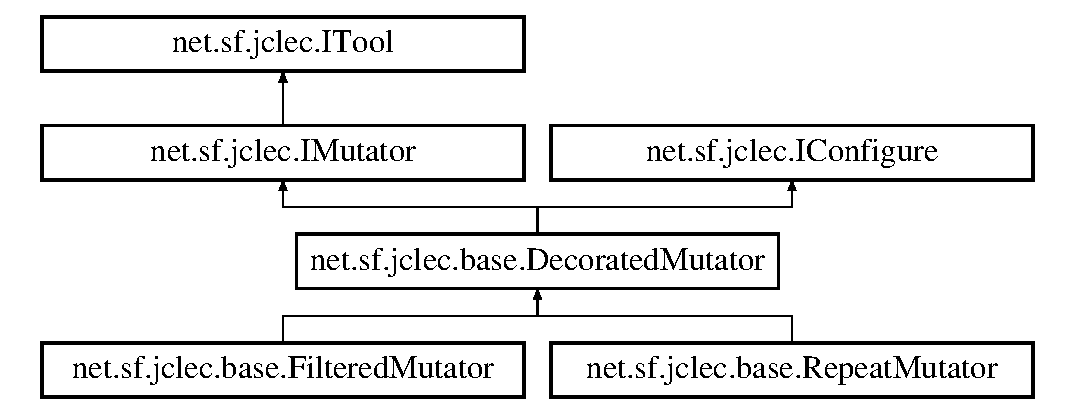
\includegraphics[height=4.000000cm]{classnet_1_1sf_1_1jclec_1_1base_1_1_decorated_mutator}
\end{center}
\end{figure}
\subsection*{Public Member Functions}
\begin{DoxyCompactItemize}
\item 
\hyperlink{classnet_1_1sf_1_1jclec_1_1base_1_1_decorated_mutator_a6091a9e583a04f96f98b5810e20a49ab}{Decorated\-Mutator} ()
\item 
\hyperlink{classnet_1_1sf_1_1jclec_1_1base_1_1_decorated_mutator_a766220134e18586517674ea963ff615e}{Decorated\-Mutator} (\hyperlink{interfacenet_1_1sf_1_1jclec_1_1_i_system}{I\-System} \hyperlink{classnet_1_1sf_1_1jclec_1_1base_1_1_decorated_mutator_a0f500ae1072a9663fa96475891c074bc}{context})
\item 
final \hyperlink{interfacenet_1_1sf_1_1jclec_1_1_i_mutator}{I\-Mutator} \hyperlink{classnet_1_1sf_1_1jclec_1_1base_1_1_decorated_mutator_a36fe66cf5bbef0c2bbdfcda114b99114}{get\-Decorated} ()
\item 
final void \hyperlink{classnet_1_1sf_1_1jclec_1_1base_1_1_decorated_mutator_ab6a4ff6195fe23e50bb296b0452aa8ba}{set\-Decorated} (\hyperlink{interfacenet_1_1sf_1_1jclec_1_1_i_mutator}{I\-Mutator} \hyperlink{classnet_1_1sf_1_1jclec_1_1base_1_1_decorated_mutator_a3eb423e738412ac288f0b37381e685f2}{decorated})
\item 
void \hyperlink{classnet_1_1sf_1_1jclec_1_1base_1_1_decorated_mutator_afa0585c251b1363b8064956f5d2d6d25}{contextualize} (\hyperlink{interfacenet_1_1sf_1_1jclec_1_1_i_system}{I\-System} \hyperlink{classnet_1_1sf_1_1jclec_1_1base_1_1_decorated_mutator_a0f500ae1072a9663fa96475891c074bc}{context})
\item 
void \hyperlink{classnet_1_1sf_1_1jclec_1_1base_1_1_decorated_mutator_ab8d9f3e1c6ac1dc1850adbdc7f979c60}{configure} (Configuration settings)
\end{DoxyCompactItemize}
\subsection*{Protected Attributes}
\begin{DoxyCompactItemize}
\item 
\hyperlink{interfacenet_1_1sf_1_1jclec_1_1_i_mutator}{I\-Mutator} \hyperlink{classnet_1_1sf_1_1jclec_1_1base_1_1_decorated_mutator_a3eb423e738412ac288f0b37381e685f2}{decorated}
\item 
\hyperlink{interfacenet_1_1sf_1_1jclec_1_1_i_system}{I\-System} \hyperlink{classnet_1_1sf_1_1jclec_1_1base_1_1_decorated_mutator_a0f500ae1072a9663fa96475891c074bc}{context}
\end{DoxyCompactItemize}


\subsection{Detailed Description}
Decorated mutator.

\begin{DoxyAuthor}{Author}
Sebastian Ventura 
\end{DoxyAuthor}


\subsection{Constructor \& Destructor Documentation}
\hypertarget{classnet_1_1sf_1_1jclec_1_1base_1_1_decorated_mutator_a6091a9e583a04f96f98b5810e20a49ab}{\index{net\-::sf\-::jclec\-::base\-::\-Decorated\-Mutator@{net\-::sf\-::jclec\-::base\-::\-Decorated\-Mutator}!Decorated\-Mutator@{Decorated\-Mutator}}
\index{Decorated\-Mutator@{Decorated\-Mutator}!net::sf::jclec::base::DecoratedMutator@{net\-::sf\-::jclec\-::base\-::\-Decorated\-Mutator}}
\subsubsection[{Decorated\-Mutator}]{\setlength{\rightskip}{0pt plus 5cm}net.\-sf.\-jclec.\-base.\-Decorated\-Mutator.\-Decorated\-Mutator (
\begin{DoxyParamCaption}
{}
\end{DoxyParamCaption}
)}}\label{classnet_1_1sf_1_1jclec_1_1base_1_1_decorated_mutator_a6091a9e583a04f96f98b5810e20a49ab}
Empty constructor \hypertarget{classnet_1_1sf_1_1jclec_1_1base_1_1_decorated_mutator_a766220134e18586517674ea963ff615e}{\index{net\-::sf\-::jclec\-::base\-::\-Decorated\-Mutator@{net\-::sf\-::jclec\-::base\-::\-Decorated\-Mutator}!Decorated\-Mutator@{Decorated\-Mutator}}
\index{Decorated\-Mutator@{Decorated\-Mutator}!net::sf::jclec::base::DecoratedMutator@{net\-::sf\-::jclec\-::base\-::\-Decorated\-Mutator}}
\subsubsection[{Decorated\-Mutator}]{\setlength{\rightskip}{0pt plus 5cm}net.\-sf.\-jclec.\-base.\-Decorated\-Mutator.\-Decorated\-Mutator (
\begin{DoxyParamCaption}
\item[{{\bf I\-System}}]{context}
\end{DoxyParamCaption}
)}}\label{classnet_1_1sf_1_1jclec_1_1base_1_1_decorated_mutator_a766220134e18586517674ea963ff615e}
Constructor that contextualizes this mutator


\begin{DoxyParams}{Parameters}
{\em context} & New execution context \\
\hline
\end{DoxyParams}


\subsection{Member Function Documentation}
\hypertarget{classnet_1_1sf_1_1jclec_1_1base_1_1_decorated_mutator_ab8d9f3e1c6ac1dc1850adbdc7f979c60}{\index{net\-::sf\-::jclec\-::base\-::\-Decorated\-Mutator@{net\-::sf\-::jclec\-::base\-::\-Decorated\-Mutator}!configure@{configure}}
\index{configure@{configure}!net::sf::jclec::base::DecoratedMutator@{net\-::sf\-::jclec\-::base\-::\-Decorated\-Mutator}}
\subsubsection[{configure}]{\setlength{\rightskip}{0pt plus 5cm}void net.\-sf.\-jclec.\-base.\-Decorated\-Mutator.\-configure (
\begin{DoxyParamCaption}
\item[{Configuration}]{settings}
\end{DoxyParamCaption}
)}}\label{classnet_1_1sf_1_1jclec_1_1base_1_1_decorated_mutator_ab8d9f3e1c6ac1dc1850adbdc7f979c60}
Configuration parameters for \hyperlink{classnet_1_1sf_1_1jclec_1_1base_1_1_decorated_mutator}{Decorated\-Mutator} are\-:


\begin{DoxyItemize}
\item {\ttfamily decorated\-: complex ... }  
\end{DoxyItemize}

Implements \hyperlink{interfacenet_1_1sf_1_1jclec_1_1_i_configure_add31a65a04d148c690a956fbbad6987c}{net.\-sf.\-jclec.\-I\-Configure}.

\hypertarget{classnet_1_1sf_1_1jclec_1_1base_1_1_decorated_mutator_afa0585c251b1363b8064956f5d2d6d25}{\index{net\-::sf\-::jclec\-::base\-::\-Decorated\-Mutator@{net\-::sf\-::jclec\-::base\-::\-Decorated\-Mutator}!contextualize@{contextualize}}
\index{contextualize@{contextualize}!net::sf::jclec::base::DecoratedMutator@{net\-::sf\-::jclec\-::base\-::\-Decorated\-Mutator}}
\subsubsection[{contextualize}]{\setlength{\rightskip}{0pt plus 5cm}void net.\-sf.\-jclec.\-base.\-Decorated\-Mutator.\-contextualize (
\begin{DoxyParamCaption}
\item[{{\bf I\-System}}]{context}
\end{DoxyParamCaption}
)}}\label{classnet_1_1sf_1_1jclec_1_1base_1_1_decorated_mutator_afa0585c251b1363b8064956f5d2d6d25}
Contextualize decorated mutator (if exists)

Set the system where ...


\begin{DoxyParams}{Parameters}
{\em context} & Execution context\\
\hline
\end{DoxyParams}
 

Implements \hyperlink{interfacenet_1_1sf_1_1jclec_1_1_i_tool_aa11b3e046b7f38e40eb4f8c72a9a2102}{net.\-sf.\-jclec.\-I\-Tool}.

\hypertarget{classnet_1_1sf_1_1jclec_1_1base_1_1_decorated_mutator_a36fe66cf5bbef0c2bbdfcda114b99114}{\index{net\-::sf\-::jclec\-::base\-::\-Decorated\-Mutator@{net\-::sf\-::jclec\-::base\-::\-Decorated\-Mutator}!get\-Decorated@{get\-Decorated}}
\index{get\-Decorated@{get\-Decorated}!net::sf::jclec::base::DecoratedMutator@{net\-::sf\-::jclec\-::base\-::\-Decorated\-Mutator}}
\subsubsection[{get\-Decorated}]{\setlength{\rightskip}{0pt plus 5cm}final {\bf I\-Mutator} net.\-sf.\-jclec.\-base.\-Decorated\-Mutator.\-get\-Decorated (
\begin{DoxyParamCaption}
{}
\end{DoxyParamCaption}
)}}\label{classnet_1_1sf_1_1jclec_1_1base_1_1_decorated_mutator_a36fe66cf5bbef0c2bbdfcda114b99114}
Access to decorated mutator.

\begin{DoxyReturn}{Returns}
Decorated mutator 
\end{DoxyReturn}
\hypertarget{classnet_1_1sf_1_1jclec_1_1base_1_1_decorated_mutator_ab6a4ff6195fe23e50bb296b0452aa8ba}{\index{net\-::sf\-::jclec\-::base\-::\-Decorated\-Mutator@{net\-::sf\-::jclec\-::base\-::\-Decorated\-Mutator}!set\-Decorated@{set\-Decorated}}
\index{set\-Decorated@{set\-Decorated}!net::sf::jclec::base::DecoratedMutator@{net\-::sf\-::jclec\-::base\-::\-Decorated\-Mutator}}
\subsubsection[{set\-Decorated}]{\setlength{\rightskip}{0pt plus 5cm}final void net.\-sf.\-jclec.\-base.\-Decorated\-Mutator.\-set\-Decorated (
\begin{DoxyParamCaption}
\item[{{\bf I\-Mutator}}]{decorated}
\end{DoxyParamCaption}
)}}\label{classnet_1_1sf_1_1jclec_1_1base_1_1_decorated_mutator_ab6a4ff6195fe23e50bb296b0452aa8ba}
Set the mutator to decorate


\begin{DoxyParams}{Parameters}
{\em decorated} & Mutator to decorate \\
\hline
\end{DoxyParams}


\subsection{Member Data Documentation}
\hypertarget{classnet_1_1sf_1_1jclec_1_1base_1_1_decorated_mutator_a0f500ae1072a9663fa96475891c074bc}{\index{net\-::sf\-::jclec\-::base\-::\-Decorated\-Mutator@{net\-::sf\-::jclec\-::base\-::\-Decorated\-Mutator}!context@{context}}
\index{context@{context}!net::sf::jclec::base::DecoratedMutator@{net\-::sf\-::jclec\-::base\-::\-Decorated\-Mutator}}
\subsubsection[{context}]{\setlength{\rightskip}{0pt plus 5cm}{\bf I\-System} net.\-sf.\-jclec.\-base.\-Decorated\-Mutator.\-context\hspace{0.3cm}{\ttfamily [protected]}}}\label{classnet_1_1sf_1_1jclec_1_1base_1_1_decorated_mutator_a0f500ae1072a9663fa96475891c074bc}
Execution context \hypertarget{classnet_1_1sf_1_1jclec_1_1base_1_1_decorated_mutator_a3eb423e738412ac288f0b37381e685f2}{\index{net\-::sf\-::jclec\-::base\-::\-Decorated\-Mutator@{net\-::sf\-::jclec\-::base\-::\-Decorated\-Mutator}!decorated@{decorated}}
\index{decorated@{decorated}!net::sf::jclec::base::DecoratedMutator@{net\-::sf\-::jclec\-::base\-::\-Decorated\-Mutator}}
\subsubsection[{decorated}]{\setlength{\rightskip}{0pt plus 5cm}{\bf I\-Mutator} net.\-sf.\-jclec.\-base.\-Decorated\-Mutator.\-decorated\hspace{0.3cm}{\ttfamily [protected]}}}\label{classnet_1_1sf_1_1jclec_1_1base_1_1_decorated_mutator_a3eb423e738412ac288f0b37381e685f2}
Mutator to decorate 

The documentation for this class was generated from the following file\-:\begin{DoxyCompactItemize}
\item 
src/main/java/net/sf/jclec/base/Decorated\-Mutator.\-java\end{DoxyCompactItemize}

\hypertarget{classnet_1_1sf_1_1jclec_1_1base_1_1_decorated_recombinator}{\section{net.\-sf.\-jclec.\-base.\-Decorated\-Recombinator Class Reference}
\label{classnet_1_1sf_1_1jclec_1_1base_1_1_decorated_recombinator}\index{net.\-sf.\-jclec.\-base.\-Decorated\-Recombinator@{net.\-sf.\-jclec.\-base.\-Decorated\-Recombinator}}
}
Inheritance diagram for net.\-sf.\-jclec.\-base.\-Decorated\-Recombinator\-:\begin{figure}[H]
\begin{center}
\leavevmode
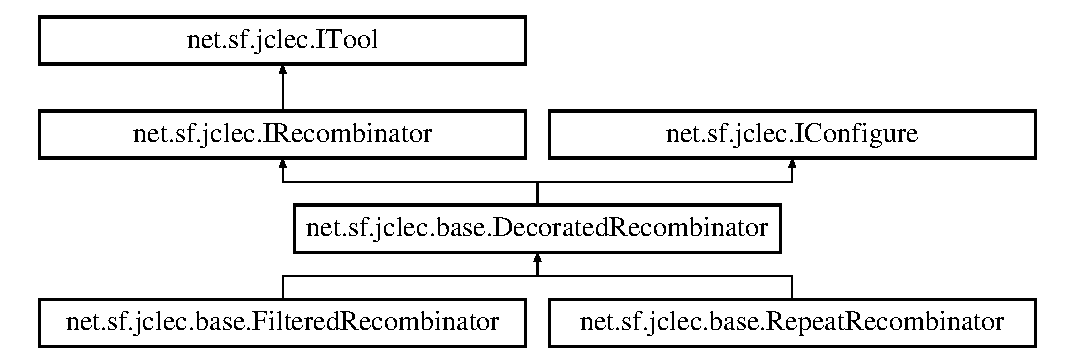
\includegraphics[height=4.000000cm]{classnet_1_1sf_1_1jclec_1_1base_1_1_decorated_recombinator}
\end{center}
\end{figure}
\subsection*{Public Member Functions}
\begin{DoxyCompactItemize}
\item 
\hyperlink{classnet_1_1sf_1_1jclec_1_1base_1_1_decorated_recombinator_a2409eb5a636fc66ef782d49bcda12767}{Decorated\-Recombinator} ()
\item 
\hyperlink{classnet_1_1sf_1_1jclec_1_1base_1_1_decorated_recombinator_aa2fcd9e6eee89cea84c0410a7cbaf877}{Decorated\-Recombinator} (\hyperlink{interfacenet_1_1sf_1_1jclec_1_1_i_system}{I\-System} \hyperlink{classnet_1_1sf_1_1jclec_1_1base_1_1_decorated_recombinator_a9fec99558ae7ddcf3ce82d8293305786}{context})
\item 
final \hyperlink{interfacenet_1_1sf_1_1jclec_1_1_i_recombinator}{I\-Recombinator} \hyperlink{classnet_1_1sf_1_1jclec_1_1base_1_1_decorated_recombinator_a52c12c467b530190e619be015133979f}{get\-Decorated} ()
\item 
final void \hyperlink{classnet_1_1sf_1_1jclec_1_1base_1_1_decorated_recombinator_a9e8c354c25cfadcf221756dfc197d660}{set\-Decorated} (\hyperlink{interfacenet_1_1sf_1_1jclec_1_1_i_recombinator}{I\-Recombinator} \hyperlink{classnet_1_1sf_1_1jclec_1_1base_1_1_decorated_recombinator_a525eba528ff918e1be5d29d74cefb614}{decorated})
\item 
void \hyperlink{classnet_1_1sf_1_1jclec_1_1base_1_1_decorated_recombinator_a422262d71b7e49d04f11cf0d655278b2}{contextualize} (\hyperlink{interfacenet_1_1sf_1_1jclec_1_1_i_system}{I\-System} \hyperlink{classnet_1_1sf_1_1jclec_1_1base_1_1_decorated_recombinator_a9fec99558ae7ddcf3ce82d8293305786}{context})
\item 
final int \hyperlink{classnet_1_1sf_1_1jclec_1_1base_1_1_decorated_recombinator_adf1ac2852510fb9752ffc7bd01634748}{get\-Ppl} ()
\item 
final int \hyperlink{classnet_1_1sf_1_1jclec_1_1base_1_1_decorated_recombinator_a1c7ff213d34427145b5332c4df3292a9}{get\-Spl} ()
\item 
void \hyperlink{classnet_1_1sf_1_1jclec_1_1base_1_1_decorated_recombinator_acec6cc90c1f13341f8087029b588797c}{configure} (Configuration settings)
\end{DoxyCompactItemize}
\subsection*{Protected Attributes}
\begin{DoxyCompactItemize}
\item 
\hyperlink{interfacenet_1_1sf_1_1jclec_1_1_i_recombinator}{I\-Recombinator} \hyperlink{classnet_1_1sf_1_1jclec_1_1base_1_1_decorated_recombinator_a525eba528ff918e1be5d29d74cefb614}{decorated}
\item 
\hyperlink{interfacenet_1_1sf_1_1jclec_1_1_i_system}{I\-System} \hyperlink{classnet_1_1sf_1_1jclec_1_1base_1_1_decorated_recombinator_a9fec99558ae7ddcf3ce82d8293305786}{context}
\end{DoxyCompactItemize}


\subsection{Detailed Description}
Decorated recombinator.

\begin{DoxyAuthor}{Author}
Sebastian Ventura 
\end{DoxyAuthor}


\subsection{Constructor \& Destructor Documentation}
\hypertarget{classnet_1_1sf_1_1jclec_1_1base_1_1_decorated_recombinator_a2409eb5a636fc66ef782d49bcda12767}{\index{net\-::sf\-::jclec\-::base\-::\-Decorated\-Recombinator@{net\-::sf\-::jclec\-::base\-::\-Decorated\-Recombinator}!Decorated\-Recombinator@{Decorated\-Recombinator}}
\index{Decorated\-Recombinator@{Decorated\-Recombinator}!net::sf::jclec::base::DecoratedRecombinator@{net\-::sf\-::jclec\-::base\-::\-Decorated\-Recombinator}}
\subsubsection[{Decorated\-Recombinator}]{\setlength{\rightskip}{0pt plus 5cm}net.\-sf.\-jclec.\-base.\-Decorated\-Recombinator.\-Decorated\-Recombinator (
\begin{DoxyParamCaption}
{}
\end{DoxyParamCaption}
)}}\label{classnet_1_1sf_1_1jclec_1_1base_1_1_decorated_recombinator_a2409eb5a636fc66ef782d49bcda12767}
Empty constructor \hypertarget{classnet_1_1sf_1_1jclec_1_1base_1_1_decorated_recombinator_aa2fcd9e6eee89cea84c0410a7cbaf877}{\index{net\-::sf\-::jclec\-::base\-::\-Decorated\-Recombinator@{net\-::sf\-::jclec\-::base\-::\-Decorated\-Recombinator}!Decorated\-Recombinator@{Decorated\-Recombinator}}
\index{Decorated\-Recombinator@{Decorated\-Recombinator}!net::sf::jclec::base::DecoratedRecombinator@{net\-::sf\-::jclec\-::base\-::\-Decorated\-Recombinator}}
\subsubsection[{Decorated\-Recombinator}]{\setlength{\rightskip}{0pt plus 5cm}net.\-sf.\-jclec.\-base.\-Decorated\-Recombinator.\-Decorated\-Recombinator (
\begin{DoxyParamCaption}
\item[{{\bf I\-System}}]{context}
\end{DoxyParamCaption}
)}}\label{classnet_1_1sf_1_1jclec_1_1base_1_1_decorated_recombinator_aa2fcd9e6eee89cea84c0410a7cbaf877}
Constructor that contextualizes this recombinator


\begin{DoxyParams}{Parameters}
{\em context} & New execution context \\
\hline
\end{DoxyParams}


\subsection{Member Function Documentation}
\hypertarget{classnet_1_1sf_1_1jclec_1_1base_1_1_decorated_recombinator_acec6cc90c1f13341f8087029b588797c}{\index{net\-::sf\-::jclec\-::base\-::\-Decorated\-Recombinator@{net\-::sf\-::jclec\-::base\-::\-Decorated\-Recombinator}!configure@{configure}}
\index{configure@{configure}!net::sf::jclec::base::DecoratedRecombinator@{net\-::sf\-::jclec\-::base\-::\-Decorated\-Recombinator}}
\subsubsection[{configure}]{\setlength{\rightskip}{0pt plus 5cm}void net.\-sf.\-jclec.\-base.\-Decorated\-Recombinator.\-configure (
\begin{DoxyParamCaption}
\item[{Configuration}]{settings}
\end{DoxyParamCaption}
)}}\label{classnet_1_1sf_1_1jclec_1_1base_1_1_decorated_recombinator_acec6cc90c1f13341f8087029b588797c}
Configuration parameters for \hyperlink{classnet_1_1sf_1_1jclec_1_1base_1_1_decorated_recombinator}{Decorated\-Recombinator} are\-:


\begin{DoxyItemize}
\item {\ttfamily decorated\-: complex ... }  
\end{DoxyItemize}

Implements \hyperlink{interfacenet_1_1sf_1_1jclec_1_1_i_configure_add31a65a04d148c690a956fbbad6987c}{net.\-sf.\-jclec.\-I\-Configure}.

\hypertarget{classnet_1_1sf_1_1jclec_1_1base_1_1_decorated_recombinator_a422262d71b7e49d04f11cf0d655278b2}{\index{net\-::sf\-::jclec\-::base\-::\-Decorated\-Recombinator@{net\-::sf\-::jclec\-::base\-::\-Decorated\-Recombinator}!contextualize@{contextualize}}
\index{contextualize@{contextualize}!net::sf::jclec::base::DecoratedRecombinator@{net\-::sf\-::jclec\-::base\-::\-Decorated\-Recombinator}}
\subsubsection[{contextualize}]{\setlength{\rightskip}{0pt plus 5cm}void net.\-sf.\-jclec.\-base.\-Decorated\-Recombinator.\-contextualize (
\begin{DoxyParamCaption}
\item[{{\bf I\-System}}]{context}
\end{DoxyParamCaption}
)}}\label{classnet_1_1sf_1_1jclec_1_1base_1_1_decorated_recombinator_a422262d71b7e49d04f11cf0d655278b2}
Contextualize decorated mutator (if exists)

Set the system where ...


\begin{DoxyParams}{Parameters}
{\em context} & Execution context\\
\hline
\end{DoxyParams}
 

Implements \hyperlink{interfacenet_1_1sf_1_1jclec_1_1_i_tool_aa11b3e046b7f38e40eb4f8c72a9a2102}{net.\-sf.\-jclec.\-I\-Tool}.

\hypertarget{classnet_1_1sf_1_1jclec_1_1base_1_1_decorated_recombinator_a52c12c467b530190e619be015133979f}{\index{net\-::sf\-::jclec\-::base\-::\-Decorated\-Recombinator@{net\-::sf\-::jclec\-::base\-::\-Decorated\-Recombinator}!get\-Decorated@{get\-Decorated}}
\index{get\-Decorated@{get\-Decorated}!net::sf::jclec::base::DecoratedRecombinator@{net\-::sf\-::jclec\-::base\-::\-Decorated\-Recombinator}}
\subsubsection[{get\-Decorated}]{\setlength{\rightskip}{0pt plus 5cm}final {\bf I\-Recombinator} net.\-sf.\-jclec.\-base.\-Decorated\-Recombinator.\-get\-Decorated (
\begin{DoxyParamCaption}
{}
\end{DoxyParamCaption}
)}}\label{classnet_1_1sf_1_1jclec_1_1base_1_1_decorated_recombinator_a52c12c467b530190e619be015133979f}
Access to decorated recombinator.

\begin{DoxyReturn}{Returns}
Decorated recombinator 
\end{DoxyReturn}
\hypertarget{classnet_1_1sf_1_1jclec_1_1base_1_1_decorated_recombinator_adf1ac2852510fb9752ffc7bd01634748}{\index{net\-::sf\-::jclec\-::base\-::\-Decorated\-Recombinator@{net\-::sf\-::jclec\-::base\-::\-Decorated\-Recombinator}!get\-Ppl@{get\-Ppl}}
\index{get\-Ppl@{get\-Ppl}!net::sf::jclec::base::DecoratedRecombinator@{net\-::sf\-::jclec\-::base\-::\-Decorated\-Recombinator}}
\subsubsection[{get\-Ppl}]{\setlength{\rightskip}{0pt plus 5cm}final int net.\-sf.\-jclec.\-base.\-Decorated\-Recombinator.\-get\-Ppl (
\begin{DoxyParamCaption}
{}
\end{DoxyParamCaption}
)}}\label{classnet_1_1sf_1_1jclec_1_1base_1_1_decorated_recombinator_adf1ac2852510fb9752ffc7bd01634748}
Informs about the number of parents in a litter.

\begin{DoxyReturn}{Returns}
Number of parents per litter
\end{DoxyReturn}


\begin{DoxyReturn}{Returns}
decorated.\-get\-Ppl() 
\end{DoxyReturn}


Implements \hyperlink{interfacenet_1_1sf_1_1jclec_1_1_i_recombinator_a5e9e851fc35894e4e5a53531616ed42c}{net.\-sf.\-jclec.\-I\-Recombinator}.

\hypertarget{classnet_1_1sf_1_1jclec_1_1base_1_1_decorated_recombinator_a1c7ff213d34427145b5332c4df3292a9}{\index{net\-::sf\-::jclec\-::base\-::\-Decorated\-Recombinator@{net\-::sf\-::jclec\-::base\-::\-Decorated\-Recombinator}!get\-Spl@{get\-Spl}}
\index{get\-Spl@{get\-Spl}!net::sf::jclec::base::DecoratedRecombinator@{net\-::sf\-::jclec\-::base\-::\-Decorated\-Recombinator}}
\subsubsection[{get\-Spl}]{\setlength{\rightskip}{0pt plus 5cm}final int net.\-sf.\-jclec.\-base.\-Decorated\-Recombinator.\-get\-Spl (
\begin{DoxyParamCaption}
{}
\end{DoxyParamCaption}
)}}\label{classnet_1_1sf_1_1jclec_1_1base_1_1_decorated_recombinator_a1c7ff213d34427145b5332c4df3292a9}
Informs about the number of sons per litter.

\begin{DoxyReturn}{Returns}
Number of sons per litter
\end{DoxyReturn}


\begin{DoxyReturn}{Returns}
decorated.\-get\-Spl() 
\end{DoxyReturn}


Implements \hyperlink{interfacenet_1_1sf_1_1jclec_1_1_i_recombinator_a398927d69f307ecf449ac93c9e025933}{net.\-sf.\-jclec.\-I\-Recombinator}.

\hypertarget{classnet_1_1sf_1_1jclec_1_1base_1_1_decorated_recombinator_a9e8c354c25cfadcf221756dfc197d660}{\index{net\-::sf\-::jclec\-::base\-::\-Decorated\-Recombinator@{net\-::sf\-::jclec\-::base\-::\-Decorated\-Recombinator}!set\-Decorated@{set\-Decorated}}
\index{set\-Decorated@{set\-Decorated}!net::sf::jclec::base::DecoratedRecombinator@{net\-::sf\-::jclec\-::base\-::\-Decorated\-Recombinator}}
\subsubsection[{set\-Decorated}]{\setlength{\rightskip}{0pt plus 5cm}final void net.\-sf.\-jclec.\-base.\-Decorated\-Recombinator.\-set\-Decorated (
\begin{DoxyParamCaption}
\item[{{\bf I\-Recombinator}}]{decorated}
\end{DoxyParamCaption}
)}}\label{classnet_1_1sf_1_1jclec_1_1base_1_1_decorated_recombinator_a9e8c354c25cfadcf221756dfc197d660}
Set the mutator to decorate


\begin{DoxyParams}{Parameters}
{\em decorated} & Mutator to decorate \\
\hline
\end{DoxyParams}


\subsection{Member Data Documentation}
\hypertarget{classnet_1_1sf_1_1jclec_1_1base_1_1_decorated_recombinator_a9fec99558ae7ddcf3ce82d8293305786}{\index{net\-::sf\-::jclec\-::base\-::\-Decorated\-Recombinator@{net\-::sf\-::jclec\-::base\-::\-Decorated\-Recombinator}!context@{context}}
\index{context@{context}!net::sf::jclec::base::DecoratedRecombinator@{net\-::sf\-::jclec\-::base\-::\-Decorated\-Recombinator}}
\subsubsection[{context}]{\setlength{\rightskip}{0pt plus 5cm}{\bf I\-System} net.\-sf.\-jclec.\-base.\-Decorated\-Recombinator.\-context\hspace{0.3cm}{\ttfamily [protected]}}}\label{classnet_1_1sf_1_1jclec_1_1base_1_1_decorated_recombinator_a9fec99558ae7ddcf3ce82d8293305786}
Execution context \hypertarget{classnet_1_1sf_1_1jclec_1_1base_1_1_decorated_recombinator_a525eba528ff918e1be5d29d74cefb614}{\index{net\-::sf\-::jclec\-::base\-::\-Decorated\-Recombinator@{net\-::sf\-::jclec\-::base\-::\-Decorated\-Recombinator}!decorated@{decorated}}
\index{decorated@{decorated}!net::sf::jclec::base::DecoratedRecombinator@{net\-::sf\-::jclec\-::base\-::\-Decorated\-Recombinator}}
\subsubsection[{decorated}]{\setlength{\rightskip}{0pt plus 5cm}{\bf I\-Recombinator} net.\-sf.\-jclec.\-base.\-Decorated\-Recombinator.\-decorated\hspace{0.3cm}{\ttfamily [protected]}}}\label{classnet_1_1sf_1_1jclec_1_1base_1_1_decorated_recombinator_a525eba528ff918e1be5d29d74cefb614}
Recombinator to decorate 

The documentation for this class was generated from the following file\-:\begin{DoxyCompactItemize}
\item 
src/main/java/net/sf/jclec/base/Decorated\-Recombinator.\-java\end{DoxyCompactItemize}

\hypertarget{classnet_1_1sf_1_1jclec_1_1exprtree_1_1mut_1_1_demote_mutator}{\section{net.\-sf.\-jclec.\-exprtree.\-mut.\-Demote\-Mutator Class Reference}
\label{classnet_1_1sf_1_1jclec_1_1exprtree_1_1mut_1_1_demote_mutator}\index{net.\-sf.\-jclec.\-exprtree.\-mut.\-Demote\-Mutator@{net.\-sf.\-jclec.\-exprtree.\-mut.\-Demote\-Mutator}}
}
Inheritance diagram for net.\-sf.\-jclec.\-exprtree.\-mut.\-Demote\-Mutator\-:\begin{figure}[H]
\begin{center}
\leavevmode
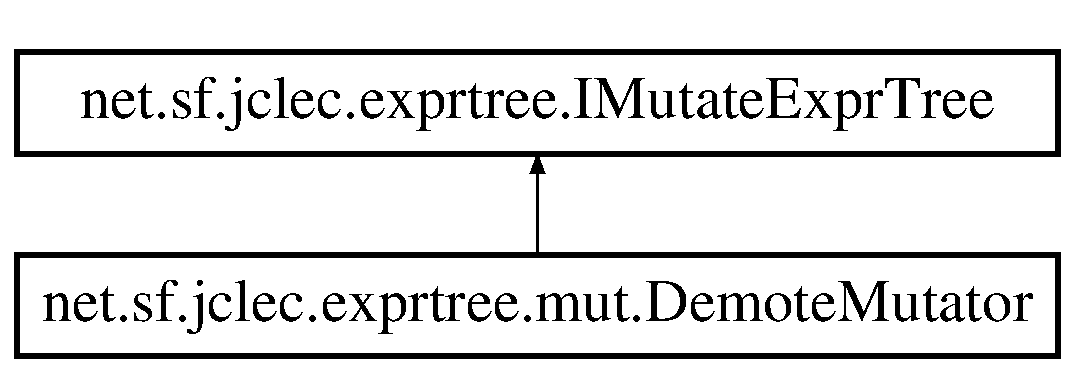
\includegraphics[height=2.000000cm]{classnet_1_1sf_1_1jclec_1_1exprtree_1_1mut_1_1_demote_mutator}
\end{center}
\end{figure}
\subsection*{Public Member Functions}
\begin{DoxyCompactItemize}
\item 
\hyperlink{classnet_1_1sf_1_1jclec_1_1exprtree_1_1_expr_tree}{Expr\-Tree} \hyperlink{classnet_1_1sf_1_1jclec_1_1exprtree_1_1mut_1_1_demote_mutator_a27bf3139df5f67ed273e0c0c3248b22c}{mutate\-Expr\-Tree} (\hyperlink{classnet_1_1sf_1_1jclec_1_1exprtree_1_1_expr_tree}{Expr\-Tree} ptree, \hyperlink{classnet_1_1sf_1_1jclec_1_1exprtree_1_1_expr_tree_schema}{Expr\-Tree\-Schema} schema, \hyperlink{interfacenet_1_1sf_1_1jclec_1_1util_1_1random_1_1_i_rand_gen}{I\-Rand\-Gen} randgen)
\end{DoxyCompactItemize}
\subsection*{Protected Member Functions}
\begin{DoxyCompactItemize}
\item 
void \hyperlink{classnet_1_1sf_1_1jclec_1_1exprtree_1_1mut_1_1_demote_mutator_abd3adfb71aea9f1091c53516b5233826}{add\-Largest\-Children} (\hyperlink{classnet_1_1sf_1_1jclec_1_1exprtree_1_1_expr_tree}{Expr\-Tree} ptree, \hyperlink{classnet_1_1sf_1_1jclec_1_1exprtree_1_1_expr_tree}{Expr\-Tree} stree, int start, \hyperlink{interfacenet_1_1sf_1_1jclec_1_1util_1_1random_1_1_i_rand_gen}{I\-Rand\-Gen} randgen)
\end{DoxyCompactItemize}


\subsection{Detailed Description}
Randomly selected a function node, replacing it with its larger son.

\begin{DoxyAuthor}{Author}
Sebastian Ventura 
\end{DoxyAuthor}


\subsection{Member Function Documentation}
\hypertarget{classnet_1_1sf_1_1jclec_1_1exprtree_1_1mut_1_1_demote_mutator_abd3adfb71aea9f1091c53516b5233826}{\index{net\-::sf\-::jclec\-::exprtree\-::mut\-::\-Demote\-Mutator@{net\-::sf\-::jclec\-::exprtree\-::mut\-::\-Demote\-Mutator}!add\-Largest\-Children@{add\-Largest\-Children}}
\index{add\-Largest\-Children@{add\-Largest\-Children}!net::sf::jclec::exprtree::mut::DemoteMutator@{net\-::sf\-::jclec\-::exprtree\-::mut\-::\-Demote\-Mutator}}
\subsubsection[{add\-Largest\-Children}]{\setlength{\rightskip}{0pt plus 5cm}void net.\-sf.\-jclec.\-exprtree.\-mut.\-Demote\-Mutator.\-add\-Largest\-Children (
\begin{DoxyParamCaption}
\item[{{\bf Expr\-Tree}}]{ptree, }
\item[{{\bf Expr\-Tree}}]{stree, }
\item[{int}]{start, }
\item[{{\bf I\-Rand\-Gen}}]{randgen}
\end{DoxyParamCaption}
)\hspace{0.3cm}{\ttfamily [protected]}}}\label{classnet_1_1sf_1_1jclec_1_1exprtree_1_1mut_1_1_demote_mutator_abd3adfb71aea9f1091c53516b5233826}
...


\begin{DoxyParams}{Parameters}
{\em ptree} & Tree parent \\
\hline
{\em stree} & Tree son \\
\hline
{\em start} & Start index \\
\hline
\end{DoxyParams}
\hypertarget{classnet_1_1sf_1_1jclec_1_1exprtree_1_1mut_1_1_demote_mutator_a27bf3139df5f67ed273e0c0c3248b22c}{\index{net\-::sf\-::jclec\-::exprtree\-::mut\-::\-Demote\-Mutator@{net\-::sf\-::jclec\-::exprtree\-::mut\-::\-Demote\-Mutator}!mutate\-Expr\-Tree@{mutate\-Expr\-Tree}}
\index{mutate\-Expr\-Tree@{mutate\-Expr\-Tree}!net::sf::jclec::exprtree::mut::DemoteMutator@{net\-::sf\-::jclec\-::exprtree\-::mut\-::\-Demote\-Mutator}}
\subsubsection[{mutate\-Expr\-Tree}]{\setlength{\rightskip}{0pt plus 5cm}{\bf Expr\-Tree} net.\-sf.\-jclec.\-exprtree.\-mut.\-Demote\-Mutator.\-mutate\-Expr\-Tree (
\begin{DoxyParamCaption}
\item[{{\bf Expr\-Tree}}]{tree, }
\item[{{\bf Expr\-Tree\-Schema}}]{tree\-Schema, }
\item[{{\bf I\-Rand\-Gen}}]{randgen}
\end{DoxyParamCaption}
)\hspace{0.3cm}{\ttfamily [virtual]}}}\label{classnet_1_1sf_1_1jclec_1_1exprtree_1_1mut_1_1_demote_mutator_a27bf3139df5f67ed273e0c0c3248b22c}

\begin{DoxyParams}{Parameters}
{\em tree} & \\
\hline
{\em tree\-Schema} & \\
\hline
{\em randgen} & \\
\hline
\end{DoxyParams}
\begin{DoxyReturn}{Returns}
A new expression tree 
\end{DoxyReturn}


Implements \hyperlink{interfacenet_1_1sf_1_1jclec_1_1exprtree_1_1_i_mutate_expr_tree_aa3d6090a4580d9cd5f0e6a834df8a535}{net.\-sf.\-jclec.\-exprtree.\-I\-Mutate\-Expr\-Tree}.



The documentation for this class was generated from the following file\-:\begin{DoxyCompactItemize}
\item 
src/main/java/net/sf/jclec/exprtree/mut/Demote\-Mutator.\-java\end{DoxyCompactItemize}

\hypertarget{classnet_1_1sf_1_1jclec_1_1exprtree_1_1mut_1_1_demote_mutator_test}{\section{net.\-sf.\-jclec.\-exprtree.\-mut.\-Demote\-Mutator\-Test Class Reference}
\label{classnet_1_1sf_1_1jclec_1_1exprtree_1_1mut_1_1_demote_mutator_test}\index{net.\-sf.\-jclec.\-exprtree.\-mut.\-Demote\-Mutator\-Test@{net.\-sf.\-jclec.\-exprtree.\-mut.\-Demote\-Mutator\-Test}}
}
Inheritance diagram for net.\-sf.\-jclec.\-exprtree.\-mut.\-Demote\-Mutator\-Test\-:\begin{figure}[H]
\begin{center}
\leavevmode
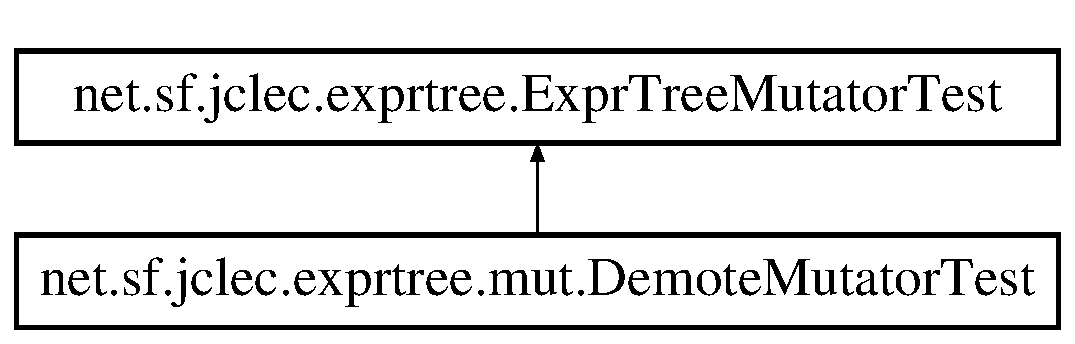
\includegraphics[height=2.000000cm]{classnet_1_1sf_1_1jclec_1_1exprtree_1_1mut_1_1_demote_mutator_test}
\end{center}
\end{figure}
\subsection*{Public Member Functions}
\begin{DoxyCompactItemize}
\item 
\hyperlink{classnet_1_1sf_1_1jclec_1_1exprtree_1_1mut_1_1_demote_mutator_test_a5a95a3ebf309c64e9ac996c54a569d5d}{Demote\-Mutator\-Test} (String name)
\end{DoxyCompactItemize}


\subsection{Detailed Description}
Unit tests for \hyperlink{classnet_1_1sf_1_1jclec_1_1exprtree_1_1mut_1_1_demote_mutator_test}{Demote\-Mutator\-Test}.

\begin{DoxyAuthor}{Author}
Amelia Zafra -\/ Sebastian Ventura 
\end{DoxyAuthor}


\subsection{Constructor \& Destructor Documentation}
\hypertarget{classnet_1_1sf_1_1jclec_1_1exprtree_1_1mut_1_1_demote_mutator_test_a5a95a3ebf309c64e9ac996c54a569d5d}{\index{net\-::sf\-::jclec\-::exprtree\-::mut\-::\-Demote\-Mutator\-Test@{net\-::sf\-::jclec\-::exprtree\-::mut\-::\-Demote\-Mutator\-Test}!Demote\-Mutator\-Test@{Demote\-Mutator\-Test}}
\index{Demote\-Mutator\-Test@{Demote\-Mutator\-Test}!net::sf::jclec::exprtree::mut::DemoteMutatorTest@{net\-::sf\-::jclec\-::exprtree\-::mut\-::\-Demote\-Mutator\-Test}}
\subsubsection[{Demote\-Mutator\-Test}]{\setlength{\rightskip}{0pt plus 5cm}net.\-sf.\-jclec.\-exprtree.\-mut.\-Demote\-Mutator\-Test.\-Demote\-Mutator\-Test (
\begin{DoxyParamCaption}
\item[{String}]{name}
\end{DoxyParamCaption}
)}}\label{classnet_1_1sf_1_1jclec_1_1exprtree_1_1mut_1_1_demote_mutator_test_a5a95a3ebf309c64e9ac996c54a569d5d}
Default constructor. 

The documentation for this class was generated from the following file\-:\begin{DoxyCompactItemize}
\item 
src/test/java/net/sf/jclec/exprtree/mut/Demote\-Mutator\-Test.\-java\end{DoxyCompactItemize}

\hypertarget{classnet_1_1sf_1_1jclec_1_1selector_1_1_deterministic_selector}{\section{net.\-sf.\-jclec.\-selector.\-Deterministic\-Selector Class Reference}
\label{classnet_1_1sf_1_1jclec_1_1selector_1_1_deterministic_selector}\index{net.\-sf.\-jclec.\-selector.\-Deterministic\-Selector@{net.\-sf.\-jclec.\-selector.\-Deterministic\-Selector}}
}
Inheritance diagram for net.\-sf.\-jclec.\-selector.\-Deterministic\-Selector\-:\begin{figure}[H]
\begin{center}
\leavevmode
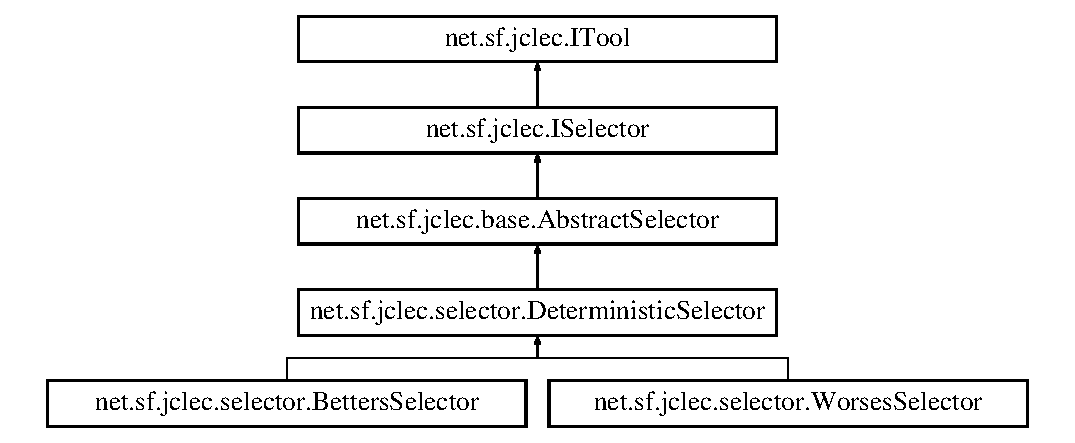
\includegraphics[height=5.000000cm]{classnet_1_1sf_1_1jclec_1_1selector_1_1_deterministic_selector}
\end{center}
\end{figure}
\subsection*{Public Member Functions}
\begin{DoxyCompactItemize}
\item 
\hyperlink{classnet_1_1sf_1_1jclec_1_1selector_1_1_deterministic_selector_a1bc263a207beaf9aa829e9eda078881f}{Deterministic\-Selector} ()
\item 
\hyperlink{classnet_1_1sf_1_1jclec_1_1selector_1_1_deterministic_selector_a475964d94625f72b2dbf473a363911b2}{Deterministic\-Selector} (\hyperlink{interfacenet_1_1sf_1_1jclec_1_1_i_system}{I\-System} \hyperlink{classnet_1_1sf_1_1jclec_1_1base_1_1_abstract_selector_a4304fe5c27aa7631dc91678d22473b94}{context})
\end{DoxyCompactItemize}
\subsection*{Additional Inherited Members}


\subsection{Detailed Description}
Deterministic selector.

\begin{DoxyAuthor}{Author}
Sebastian Ventura 
\end{DoxyAuthor}


\subsection{Constructor \& Destructor Documentation}
\hypertarget{classnet_1_1sf_1_1jclec_1_1selector_1_1_deterministic_selector_a1bc263a207beaf9aa829e9eda078881f}{\index{net\-::sf\-::jclec\-::selector\-::\-Deterministic\-Selector@{net\-::sf\-::jclec\-::selector\-::\-Deterministic\-Selector}!Deterministic\-Selector@{Deterministic\-Selector}}
\index{Deterministic\-Selector@{Deterministic\-Selector}!net::sf::jclec::selector::DeterministicSelector@{net\-::sf\-::jclec\-::selector\-::\-Deterministic\-Selector}}
\subsubsection[{Deterministic\-Selector}]{\setlength{\rightskip}{0pt plus 5cm}net.\-sf.\-jclec.\-selector.\-Deterministic\-Selector.\-Deterministic\-Selector (
\begin{DoxyParamCaption}
{}
\end{DoxyParamCaption}
)}}\label{classnet_1_1sf_1_1jclec_1_1selector_1_1_deterministic_selector_a1bc263a207beaf9aa829e9eda078881f}
Empty selector. \hypertarget{classnet_1_1sf_1_1jclec_1_1selector_1_1_deterministic_selector_a475964d94625f72b2dbf473a363911b2}{\index{net\-::sf\-::jclec\-::selector\-::\-Deterministic\-Selector@{net\-::sf\-::jclec\-::selector\-::\-Deterministic\-Selector}!Deterministic\-Selector@{Deterministic\-Selector}}
\index{Deterministic\-Selector@{Deterministic\-Selector}!net::sf::jclec::selector::DeterministicSelector@{net\-::sf\-::jclec\-::selector\-::\-Deterministic\-Selector}}
\subsubsection[{Deterministic\-Selector}]{\setlength{\rightskip}{0pt plus 5cm}net.\-sf.\-jclec.\-selector.\-Deterministic\-Selector.\-Deterministic\-Selector (
\begin{DoxyParamCaption}
\item[{{\bf I\-System}}]{context}
\end{DoxyParamCaption}
)}}\label{classnet_1_1sf_1_1jclec_1_1selector_1_1_deterministic_selector_a475964d94625f72b2dbf473a363911b2}
Empty selector. 

The documentation for this class was generated from the following file\-:\begin{DoxyCompactItemize}
\item 
src/main/java/net/sf/jclec/selector/Deterministic\-Selector.\-java\end{DoxyCompactItemize}

\hypertarget{classnet_1_1sf_1_1jclec_1_1realarray_1_1rec_1_1_discrete_crossover}{\section{net.\-sf.\-jclec.\-realarray.\-rec.\-Discrete\-Crossover Class Reference}
\label{classnet_1_1sf_1_1jclec_1_1realarray_1_1rec_1_1_discrete_crossover}\index{net.\-sf.\-jclec.\-realarray.\-rec.\-Discrete\-Crossover@{net.\-sf.\-jclec.\-realarray.\-rec.\-Discrete\-Crossover}}
}


Inherits net.\-sf.\-jclec.\-realarray.\-rec.\-Uniform\-Crossover2x2.

\subsection*{Public Member Functions}
\begin{DoxyCompactItemize}
\item 
\hyperlink{classnet_1_1sf_1_1jclec_1_1realarray_1_1rec_1_1_discrete_crossover_a0a377b112bf90cf286219321cc9a4315}{Discrete\-Crossover} ()
\end{DoxyCompactItemize}
\subsection*{Protected Member Functions}
\begin{DoxyCompactItemize}
\item 
double \hyperlink{classnet_1_1sf_1_1jclec_1_1realarray_1_1rec_1_1_discrete_crossover_aa16427826e1cd4c046f6c0049f8fe68f}{default\-Locus\-Rec\-Prob} ()
\end{DoxyCompactItemize}
\subsection*{Additional Inherited Members}


\subsection{Detailed Description}
Apply a discrete crossover for two individuals

\begin{DoxyAuthor}{Author}
Alberto Lamarca 

Sebastian Ventura 
\end{DoxyAuthor}


\subsection{Constructor \& Destructor Documentation}
\hypertarget{classnet_1_1sf_1_1jclec_1_1realarray_1_1rec_1_1_discrete_crossover_a0a377b112bf90cf286219321cc9a4315}{\index{net\-::sf\-::jclec\-::realarray\-::rec\-::\-Discrete\-Crossover@{net\-::sf\-::jclec\-::realarray\-::rec\-::\-Discrete\-Crossover}!Discrete\-Crossover@{Discrete\-Crossover}}
\index{Discrete\-Crossover@{Discrete\-Crossover}!net::sf::jclec::realarray::rec::DiscreteCrossover@{net\-::sf\-::jclec\-::realarray\-::rec\-::\-Discrete\-Crossover}}
\subsubsection[{Discrete\-Crossover}]{\setlength{\rightskip}{0pt plus 5cm}net.\-sf.\-jclec.\-realarray.\-rec.\-Discrete\-Crossover.\-Discrete\-Crossover (
\begin{DoxyParamCaption}
{}
\end{DoxyParamCaption}
)}}\label{classnet_1_1sf_1_1jclec_1_1realarray_1_1rec_1_1_discrete_crossover_a0a377b112bf90cf286219321cc9a4315}
Empty constructor 

\subsection{Member Function Documentation}
\hypertarget{classnet_1_1sf_1_1jclec_1_1realarray_1_1rec_1_1_discrete_crossover_aa16427826e1cd4c046f6c0049f8fe68f}{\index{net\-::sf\-::jclec\-::realarray\-::rec\-::\-Discrete\-Crossover@{net\-::sf\-::jclec\-::realarray\-::rec\-::\-Discrete\-Crossover}!default\-Locus\-Rec\-Prob@{default\-Locus\-Rec\-Prob}}
\index{default\-Locus\-Rec\-Prob@{default\-Locus\-Rec\-Prob}!net::sf::jclec::realarray::rec::DiscreteCrossover@{net\-::sf\-::jclec\-::realarray\-::rec\-::\-Discrete\-Crossover}}
\subsubsection[{default\-Locus\-Rec\-Prob}]{\setlength{\rightskip}{0pt plus 5cm}double net.\-sf.\-jclec.\-realarray.\-rec.\-Discrete\-Crossover.\-default\-Locus\-Rec\-Prob (
\begin{DoxyParamCaption}
{}
\end{DoxyParamCaption}
)\hspace{0.3cm}{\ttfamily [protected]}, {\ttfamily [virtual]}}}\label{classnet_1_1sf_1_1jclec_1_1realarray_1_1rec_1_1_discrete_crossover_aa16427826e1cd4c046f6c0049f8fe68f}
Get default value for this parameter. 

Implements \hyperlink{classnet_1_1sf_1_1jclec_1_1realarray_1_1_uniform_crossover_ac427b4ae11cf8b9495625005fe5ec575}{net.\-sf.\-jclec.\-realarray.\-Uniform\-Crossover}.



The documentation for this class was generated from the following file\-:\begin{DoxyCompactItemize}
\item 
src/main/java/net/sf/jclec/realarray/rec/Discrete\-Crossover.\-java\end{DoxyCompactItemize}

\hypertarget{classnet_1_1sf_1_1jclec_1_1selector_1_1_disruptive_selector}{\section{net.\-sf.\-jclec.\-selector.\-Disruptive\-Selector Class Reference}
\label{classnet_1_1sf_1_1jclec_1_1selector_1_1_disruptive_selector}\index{net.\-sf.\-jclec.\-selector.\-Disruptive\-Selector@{net.\-sf.\-jclec.\-selector.\-Disruptive\-Selector}}
}
Inheritance diagram for net.\-sf.\-jclec.\-selector.\-Disruptive\-Selector\-:\begin{figure}[H]
\begin{center}
\leavevmode
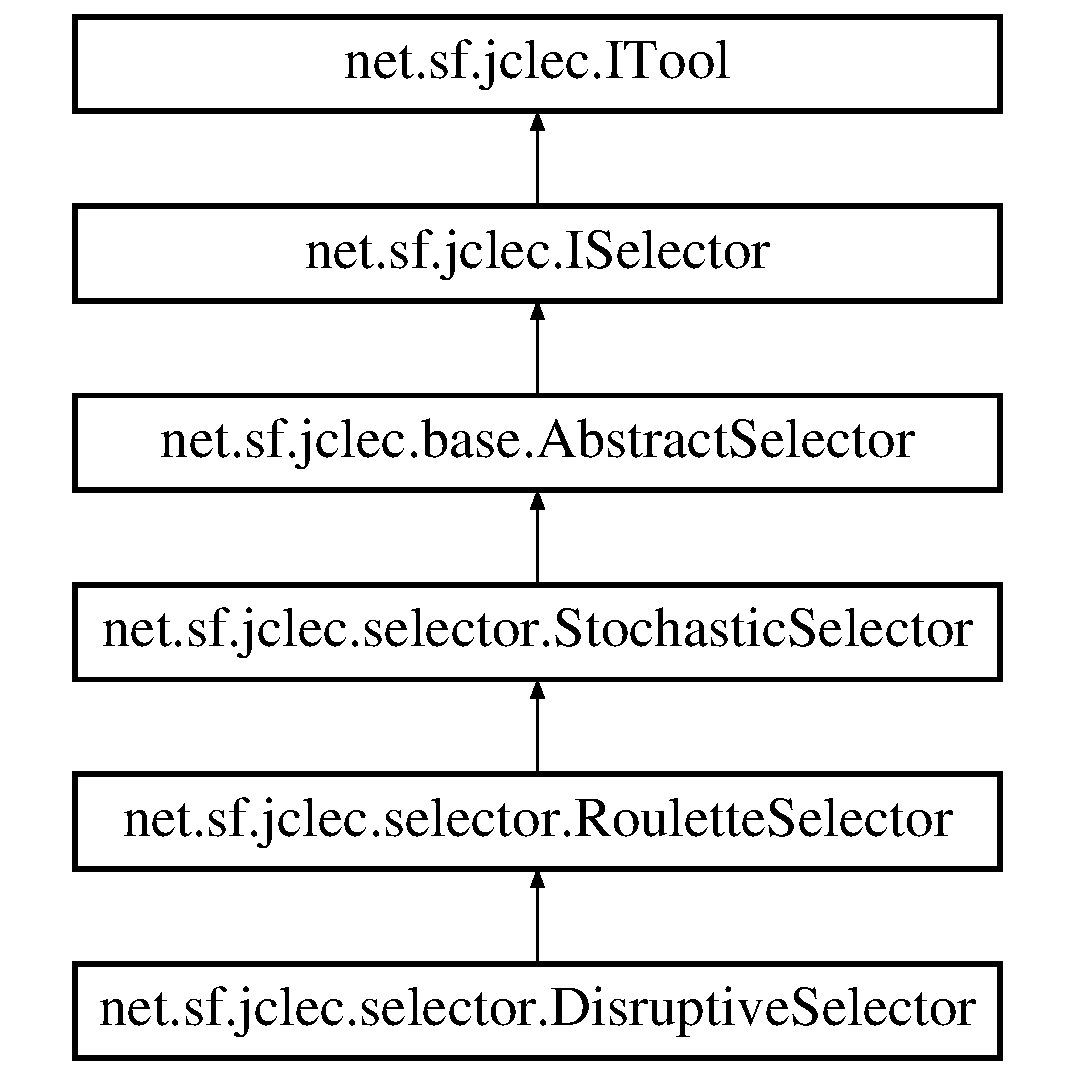
\includegraphics[height=6.000000cm]{classnet_1_1sf_1_1jclec_1_1selector_1_1_disruptive_selector}
\end{center}
\end{figure}
\subsection*{Public Member Functions}
\begin{DoxyCompactItemize}
\item 
\hyperlink{classnet_1_1sf_1_1jclec_1_1selector_1_1_disruptive_selector_ae8a25975f086bae8e3b999f21e01fa2b}{Disruptive\-Selector} ()
\item 
\hyperlink{classnet_1_1sf_1_1jclec_1_1selector_1_1_disruptive_selector_a2e61a781ef0210b0f5a4646c166e9d82}{Disruptive\-Selector} (\hyperlink{interfacenet_1_1sf_1_1jclec_1_1_i_system}{I\-System} \hyperlink{classnet_1_1sf_1_1jclec_1_1base_1_1_abstract_selector_a4304fe5c27aa7631dc91678d22473b94}{context})
\end{DoxyCompactItemize}
\subsection*{Protected Member Functions}
\begin{DoxyCompactItemize}
\item 
void \hyperlink{classnet_1_1sf_1_1jclec_1_1selector_1_1_disruptive_selector_a8f9d0833b098d9d1dc91e24804de5043}{prepare\-Selection} ()
\end{DoxyCompactItemize}
\subsection*{Additional Inherited Members}


\subsection{Detailed Description}
Disruptive selector.

\begin{DoxyAuthor}{Author}
Rafael Ayllon-\/\-Iglesias 

Sebastian Ventura 
\end{DoxyAuthor}


\subsection{Constructor \& Destructor Documentation}
\hypertarget{classnet_1_1sf_1_1jclec_1_1selector_1_1_disruptive_selector_ae8a25975f086bae8e3b999f21e01fa2b}{\index{net\-::sf\-::jclec\-::selector\-::\-Disruptive\-Selector@{net\-::sf\-::jclec\-::selector\-::\-Disruptive\-Selector}!Disruptive\-Selector@{Disruptive\-Selector}}
\index{Disruptive\-Selector@{Disruptive\-Selector}!net::sf::jclec::selector::DisruptiveSelector@{net\-::sf\-::jclec\-::selector\-::\-Disruptive\-Selector}}
\subsubsection[{Disruptive\-Selector}]{\setlength{\rightskip}{0pt plus 5cm}net.\-sf.\-jclec.\-selector.\-Disruptive\-Selector.\-Disruptive\-Selector (
\begin{DoxyParamCaption}
{}
\end{DoxyParamCaption}
)}}\label{classnet_1_1sf_1_1jclec_1_1selector_1_1_disruptive_selector_ae8a25975f086bae8e3b999f21e01fa2b}
Empty (default constructor). \hypertarget{classnet_1_1sf_1_1jclec_1_1selector_1_1_disruptive_selector_a2e61a781ef0210b0f5a4646c166e9d82}{\index{net\-::sf\-::jclec\-::selector\-::\-Disruptive\-Selector@{net\-::sf\-::jclec\-::selector\-::\-Disruptive\-Selector}!Disruptive\-Selector@{Disruptive\-Selector}}
\index{Disruptive\-Selector@{Disruptive\-Selector}!net::sf::jclec::selector::DisruptiveSelector@{net\-::sf\-::jclec\-::selector\-::\-Disruptive\-Selector}}
\subsubsection[{Disruptive\-Selector}]{\setlength{\rightskip}{0pt plus 5cm}net.\-sf.\-jclec.\-selector.\-Disruptive\-Selector.\-Disruptive\-Selector (
\begin{DoxyParamCaption}
\item[{{\bf I\-System}}]{context}
\end{DoxyParamCaption}
)}}\label{classnet_1_1sf_1_1jclec_1_1selector_1_1_disruptive_selector_a2e61a781ef0210b0f5a4646c166e9d82}
Constructor that contextualizes selector


\begin{DoxyParams}{Parameters}
{\em context} & Execution context \\
\hline
\end{DoxyParams}


\subsection{Member Function Documentation}
\hypertarget{classnet_1_1sf_1_1jclec_1_1selector_1_1_disruptive_selector_a8f9d0833b098d9d1dc91e24804de5043}{\index{net\-::sf\-::jclec\-::selector\-::\-Disruptive\-Selector@{net\-::sf\-::jclec\-::selector\-::\-Disruptive\-Selector}!prepare\-Selection@{prepare\-Selection}}
\index{prepare\-Selection@{prepare\-Selection}!net::sf::jclec::selector::DisruptiveSelector@{net\-::sf\-::jclec\-::selector\-::\-Disruptive\-Selector}}
\subsubsection[{prepare\-Selection}]{\setlength{\rightskip}{0pt plus 5cm}void net.\-sf.\-jclec.\-selector.\-Disruptive\-Selector.\-prepare\-Selection (
\begin{DoxyParamCaption}
{}
\end{DoxyParamCaption}
)\hspace{0.3cm}{\ttfamily [protected]}, {\ttfamily [virtual]}}}\label{classnet_1_1sf_1_1jclec_1_1selector_1_1_disruptive_selector_a8f9d0833b098d9d1dc91e24804de5043}
Nombre\-: prepare\-Selection Autor\-: Rafael Ayll\-A?n Iglesias. Tipo funcion\-: protegida Valores de entrada\-: Ninguno Valores de salida\-: Ninguno Funciones que utiliza\-: Ninguna Variables\-:-\/ Fitness\-Total es un double que almacena el fitness total
\begin{DoxyItemize}
\item media\-Fitness es un double que almacena la media del fitness
\item Fitness\-Normalizado\-Total es un double que almacena el fitness total normalizado
\item media\-Fitness\-Normalizado es un double que almacena la media del fitness normalizado
\item Fitness\-Normalizado es un double que almacena el fitnes normalizado
\item acc es el acumulado de las partes de la ruleta
\item idx es el indice de la ruleta Objetivo\-: Preparar las variables para la utilizacion de la ruleta 
\end{DoxyItemize}

Implements \hyperlink{classnet_1_1sf_1_1jclec_1_1base_1_1_abstract_selector_a0c5d9cb96fef9786e272b9edd811111e}{net.\-sf.\-jclec.\-base.\-Abstract\-Selector}.



The documentation for this class was generated from the following file\-:\begin{DoxyCompactItemize}
\item 
src/main/java/net/sf/jclec/selector/Disruptive\-Selector.\-java\end{DoxyCompactItemize}

\hypertarget{classnet_1_1sf_1_1jclec_1_1selector_1_1_disruptive_selector_test}{\section{net.\-sf.\-jclec.\-selector.\-Disruptive\-Selector\-Test Class Reference}
\label{classnet_1_1sf_1_1jclec_1_1selector_1_1_disruptive_selector_test}\index{net.\-sf.\-jclec.\-selector.\-Disruptive\-Selector\-Test@{net.\-sf.\-jclec.\-selector.\-Disruptive\-Selector\-Test}}
}


Inherits I\-Selector\-Test$<$ Disruptive\-Selector $>$.

\subsection*{Public Member Functions}
\begin{DoxyCompactItemize}
\item 
\hyperlink{classnet_1_1sf_1_1jclec_1_1selector_1_1_disruptive_selector_test_a423763a14101d84fb818e1304334b116}{Disruptive\-Selector\-Test} (String name)
\end{DoxyCompactItemize}


\subsection{Detailed Description}
Disruptive selector tests.

\begin{DoxyAuthor}{Author}
Rafael Aguilera 
\end{DoxyAuthor}


\subsection{Constructor \& Destructor Documentation}
\hypertarget{classnet_1_1sf_1_1jclec_1_1selector_1_1_disruptive_selector_test_a423763a14101d84fb818e1304334b116}{\index{net\-::sf\-::jclec\-::selector\-::\-Disruptive\-Selector\-Test@{net\-::sf\-::jclec\-::selector\-::\-Disruptive\-Selector\-Test}!Disruptive\-Selector\-Test@{Disruptive\-Selector\-Test}}
\index{Disruptive\-Selector\-Test@{Disruptive\-Selector\-Test}!net::sf::jclec::selector::DisruptiveSelectorTest@{net\-::sf\-::jclec\-::selector\-::\-Disruptive\-Selector\-Test}}
\subsubsection[{Disruptive\-Selector\-Test}]{\setlength{\rightskip}{0pt plus 5cm}net.\-sf.\-jclec.\-selector.\-Disruptive\-Selector\-Test.\-Disruptive\-Selector\-Test (
\begin{DoxyParamCaption}
\item[{String}]{name}
\end{DoxyParamCaption}
)}}\label{classnet_1_1sf_1_1jclec_1_1selector_1_1_disruptive_selector_test_a423763a14101d84fb818e1304334b116}
Default constructor


\begin{DoxyParams}{Parameters}
{\em name} & \\
\hline
\end{DoxyParams}


The documentation for this class was generated from the following file\-:\begin{DoxyCompactItemize}
\item 
src/test/java/net/sf/jclec/selector/Disruptive\-Selector\-Test.\-java\end{DoxyCompactItemize}

\hypertarget{classnet_1_1sf_1_1jclec_1_1util_1_1random_1_1_dummy_rand_gen}{\section{net.\-sf.\-jclec.\-util.\-random.\-Dummy\-Rand\-Gen Class Reference}
\label{classnet_1_1sf_1_1jclec_1_1util_1_1random_1_1_dummy_rand_gen}\index{net.\-sf.\-jclec.\-util.\-random.\-Dummy\-Rand\-Gen@{net.\-sf.\-jclec.\-util.\-random.\-Dummy\-Rand\-Gen}}
}
Inheritance diagram for net.\-sf.\-jclec.\-util.\-random.\-Dummy\-Rand\-Gen\-:\begin{figure}[H]
\begin{center}
\leavevmode
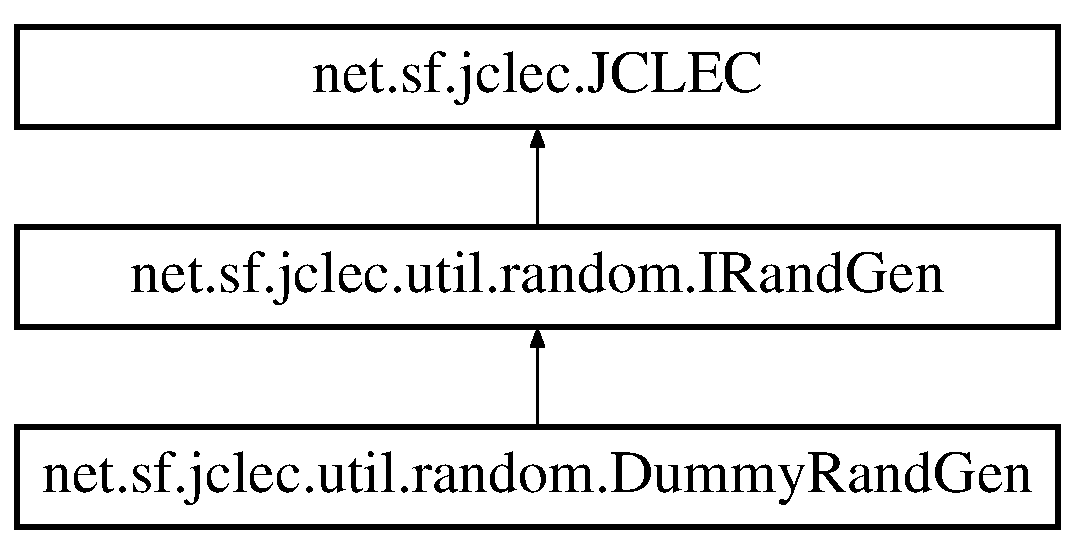
\includegraphics[height=3.000000cm]{classnet_1_1sf_1_1jclec_1_1util_1_1random_1_1_dummy_rand_gen}
\end{center}
\end{figure}
\subsection*{Public Member Functions}
\begin{DoxyCompactItemize}
\item 
\hyperlink{classnet_1_1sf_1_1jclec_1_1util_1_1random_1_1_dummy_rand_gen_a5e9875d803e71ea99886b27189794e86}{Dummy\-Rand\-Gen} ()
\item 
\hyperlink{classnet_1_1sf_1_1jclec_1_1util_1_1random_1_1_dummy_rand_gen_a9923f167a9e416f17bf9b0c265e5510b}{Dummy\-Rand\-Gen} (double\mbox{[}$\,$\mbox{]} dum\-Seq)
\item 
double\mbox{[}$\,$\mbox{]} \hyperlink{classnet_1_1sf_1_1jclec_1_1util_1_1random_1_1_dummy_rand_gen_a281ba055c9c6e0fde87bc9ae96bdab6b}{get\-Dummy\-Sequence} ()
\item 
void \hyperlink{classnet_1_1sf_1_1jclec_1_1util_1_1random_1_1_dummy_rand_gen_adac5cb50b26ef7e1a0e3faee9865e42b}{set\-Dummy\-Sequence} (double\mbox{[}$\,$\mbox{]} dum\-Seq)
\item 
double \hyperlink{classnet_1_1sf_1_1jclec_1_1util_1_1random_1_1_dummy_rand_gen_a7ecbc016777a37e970e8543c98c14d8a}{raw} ()
\item 
void \hyperlink{classnet_1_1sf_1_1jclec_1_1util_1_1random_1_1_dummy_rand_gen_a38cf447db780fada212a1e0e2b082021}{raw} (double\mbox{[}$\,$\mbox{]} d, int n)
\item 
final void \hyperlink{classnet_1_1sf_1_1jclec_1_1util_1_1random_1_1_dummy_rand_gen_a6514a30f395f08b564b6b5844bc9a5cf}{raw} (double\mbox{[}$\,$\mbox{]} d)
\item 
final int \hyperlink{classnet_1_1sf_1_1jclec_1_1util_1_1random_1_1_dummy_rand_gen_af329cf5ab656a3866eca5b32f0581e7d}{choose} (int hi)
\item 
int \hyperlink{classnet_1_1sf_1_1jclec_1_1util_1_1random_1_1_dummy_rand_gen_acc5c12a791cb81dde1cc0551b2d92ca0}{choose} (int lo, int hi)
\item 
final boolean \hyperlink{classnet_1_1sf_1_1jclec_1_1util_1_1random_1_1_dummy_rand_gen_ab1b55d5aef0efdedc8e081d79a55f73b}{coin} ()
\item 
final boolean \hyperlink{classnet_1_1sf_1_1jclec_1_1util_1_1random_1_1_dummy_rand_gen_a340eedaf204cea38f6021154088f3be1}{coin} (double p)
\item 
final double \hyperlink{classnet_1_1sf_1_1jclec_1_1util_1_1random_1_1_dummy_rand_gen_a327d55b8d886a4ea4c8b20e685ad3031}{uniform} (double lo, double hi)
\item 
final double \hyperlink{classnet_1_1sf_1_1jclec_1_1util_1_1random_1_1_dummy_rand_gen_a89e52e23a4fbc7b4ac45836012c6df39}{gaussian} ()
\item 
final double \hyperlink{classnet_1_1sf_1_1jclec_1_1util_1_1random_1_1_dummy_rand_gen_ac6416b6bcfe04c5db756eba9833be667}{gaussian} (double sd)
\item 
final double \hyperlink{classnet_1_1sf_1_1jclec_1_1util_1_1random_1_1_dummy_rand_gen_a7af42bf24cdc59f4f93d1458667739fb}{powlaw} (double alpha, double cut)
\end{DoxyCompactItemize}
\subsection*{Protected Attributes}
\begin{DoxyCompactItemize}
\item 
double\mbox{[}$\,$\mbox{]} \hyperlink{classnet_1_1sf_1_1jclec_1_1util_1_1random_1_1_dummy_rand_gen_a1b46d8d65c07d375a79cb47e93047bde}{dummy\-Sequence}
\item 
Double \hyperlink{classnet_1_1sf_1_1jclec_1_1util_1_1random_1_1_dummy_rand_gen_a5c42bd5cadb8dd6471441d1f85665d56}{B\-Moutput}
\item 
transient int \hyperlink{classnet_1_1sf_1_1jclec_1_1util_1_1random_1_1_dummy_rand_gen_ad14fb3cc2b1564fd4358239aa06dca1d}{dummy\-Sequence\-Index}
\end{DoxyCompactItemize}


\subsection{Detailed Description}
Dummy random generator.

This object ...

\begin{DoxyAuthor}{Author}
Sebastian Ventura 
\end{DoxyAuthor}


\subsection{Constructor \& Destructor Documentation}
\hypertarget{classnet_1_1sf_1_1jclec_1_1util_1_1random_1_1_dummy_rand_gen_a5e9875d803e71ea99886b27189794e86}{\index{net\-::sf\-::jclec\-::util\-::random\-::\-Dummy\-Rand\-Gen@{net\-::sf\-::jclec\-::util\-::random\-::\-Dummy\-Rand\-Gen}!Dummy\-Rand\-Gen@{Dummy\-Rand\-Gen}}
\index{Dummy\-Rand\-Gen@{Dummy\-Rand\-Gen}!net::sf::jclec::util::random::DummyRandGen@{net\-::sf\-::jclec\-::util\-::random\-::\-Dummy\-Rand\-Gen}}
\subsubsection[{Dummy\-Rand\-Gen}]{\setlength{\rightskip}{0pt plus 5cm}net.\-sf.\-jclec.\-util.\-random.\-Dummy\-Rand\-Gen.\-Dummy\-Rand\-Gen (
\begin{DoxyParamCaption}
{}
\end{DoxyParamCaption}
)}}\label{classnet_1_1sf_1_1jclec_1_1util_1_1random_1_1_dummy_rand_gen_a5e9875d803e71ea99886b27189794e86}
Empty constructor. \hypertarget{classnet_1_1sf_1_1jclec_1_1util_1_1random_1_1_dummy_rand_gen_a9923f167a9e416f17bf9b0c265e5510b}{\index{net\-::sf\-::jclec\-::util\-::random\-::\-Dummy\-Rand\-Gen@{net\-::sf\-::jclec\-::util\-::random\-::\-Dummy\-Rand\-Gen}!Dummy\-Rand\-Gen@{Dummy\-Rand\-Gen}}
\index{Dummy\-Rand\-Gen@{Dummy\-Rand\-Gen}!net::sf::jclec::util::random::DummyRandGen@{net\-::sf\-::jclec\-::util\-::random\-::\-Dummy\-Rand\-Gen}}
\subsubsection[{Dummy\-Rand\-Gen}]{\setlength{\rightskip}{0pt plus 5cm}net.\-sf.\-jclec.\-util.\-random.\-Dummy\-Rand\-Gen.\-Dummy\-Rand\-Gen (
\begin{DoxyParamCaption}
\item[{double\mbox{[}$\,$\mbox{]}}]{dum\-Seq}
\end{DoxyParamCaption}
)}}\label{classnet_1_1sf_1_1jclec_1_1util_1_1random_1_1_dummy_rand_gen_a9923f167a9e416f17bf9b0c265e5510b}
Constructor that sets generator sequence.


\begin{DoxyParams}{Parameters}
{\em dum\-Seq} & Generator Sequence \\
\hline
\end{DoxyParams}


\subsection{Member Function Documentation}
\hypertarget{classnet_1_1sf_1_1jclec_1_1util_1_1random_1_1_dummy_rand_gen_af329cf5ab656a3866eca5b32f0581e7d}{\index{net\-::sf\-::jclec\-::util\-::random\-::\-Dummy\-Rand\-Gen@{net\-::sf\-::jclec\-::util\-::random\-::\-Dummy\-Rand\-Gen}!choose@{choose}}
\index{choose@{choose}!net::sf::jclec::util::random::DummyRandGen@{net\-::sf\-::jclec\-::util\-::random\-::\-Dummy\-Rand\-Gen}}
\subsubsection[{choose}]{\setlength{\rightskip}{0pt plus 5cm}final int net.\-sf.\-jclec.\-util.\-random.\-Dummy\-Rand\-Gen.\-choose (
\begin{DoxyParamCaption}
\item[{int}]{hi}
\end{DoxyParamCaption}
)}}\label{classnet_1_1sf_1_1jclec_1_1util_1_1random_1_1_dummy_rand_gen_af329cf5ab656a3866eca5b32f0581e7d}
Return an integer random value in the range \mbox{[}1, ...hi)


\begin{DoxyParams}{Parameters}
{\em hi} & upper limit of range.\\
\hline
\end{DoxyParams}
\begin{DoxyReturn}{Returns}
a random integer in the range.
\end{DoxyReturn}
 

Implements \hyperlink{interfacenet_1_1sf_1_1jclec_1_1util_1_1random_1_1_i_rand_gen_a98171510a2905523f08ab7cfd59ddc98}{net.\-sf.\-jclec.\-util.\-random.\-I\-Rand\-Gen}.

\hypertarget{classnet_1_1sf_1_1jclec_1_1util_1_1random_1_1_dummy_rand_gen_acc5c12a791cb81dde1cc0551b2d92ca0}{\index{net\-::sf\-::jclec\-::util\-::random\-::\-Dummy\-Rand\-Gen@{net\-::sf\-::jclec\-::util\-::random\-::\-Dummy\-Rand\-Gen}!choose@{choose}}
\index{choose@{choose}!net::sf::jclec::util::random::DummyRandGen@{net\-::sf\-::jclec\-::util\-::random\-::\-Dummy\-Rand\-Gen}}
\subsubsection[{choose}]{\setlength{\rightskip}{0pt plus 5cm}int net.\-sf.\-jclec.\-util.\-random.\-Dummy\-Rand\-Gen.\-choose (
\begin{DoxyParamCaption}
\item[{int}]{lo, }
\item[{int}]{hi}
\end{DoxyParamCaption}
)}}\label{classnet_1_1sf_1_1jclec_1_1util_1_1random_1_1_dummy_rand_gen_acc5c12a791cb81dde1cc0551b2d92ca0}
Return an integer random value in the range \mbox{[}lo, ...hi)


\begin{DoxyParams}{Parameters}
{\em lo} & lower limit of range \\
\hline
{\em hi} & upper limit of range\\
\hline
\end{DoxyParams}
\begin{DoxyReturn}{Returns}
a random integer in the range.
\end{DoxyReturn}
 

Implements \hyperlink{interfacenet_1_1sf_1_1jclec_1_1util_1_1random_1_1_i_rand_gen_ac49d06156eeeea535792996b15f8b8a4}{net.\-sf.\-jclec.\-util.\-random.\-I\-Rand\-Gen}.

\hypertarget{classnet_1_1sf_1_1jclec_1_1util_1_1random_1_1_dummy_rand_gen_ab1b55d5aef0efdedc8e081d79a55f73b}{\index{net\-::sf\-::jclec\-::util\-::random\-::\-Dummy\-Rand\-Gen@{net\-::sf\-::jclec\-::util\-::random\-::\-Dummy\-Rand\-Gen}!coin@{coin}}
\index{coin@{coin}!net::sf::jclec::util::random::DummyRandGen@{net\-::sf\-::jclec\-::util\-::random\-::\-Dummy\-Rand\-Gen}}
\subsubsection[{coin}]{\setlength{\rightskip}{0pt plus 5cm}final boolean net.\-sf.\-jclec.\-util.\-random.\-Dummy\-Rand\-Gen.\-coin (
\begin{DoxyParamCaption}
{}
\end{DoxyParamCaption}
)}}\label{classnet_1_1sf_1_1jclec_1_1util_1_1random_1_1_dummy_rand_gen_ab1b55d5aef0efdedc8e081d79a55f73b}
Return a boolean that's true 0.\-5 of the time. This method call is equivalent to coin(0.\-5).

\begin{DoxyReturn}{Returns}
a boolean that's true 0.\-5 of the time.
\end{DoxyReturn}
 

Implements \hyperlink{interfacenet_1_1sf_1_1jclec_1_1util_1_1random_1_1_i_rand_gen_a59c165689aeaed76946f86e780da4bb3}{net.\-sf.\-jclec.\-util.\-random.\-I\-Rand\-Gen}.

\hypertarget{classnet_1_1sf_1_1jclec_1_1util_1_1random_1_1_dummy_rand_gen_a340eedaf204cea38f6021154088f3be1}{\index{net\-::sf\-::jclec\-::util\-::random\-::\-Dummy\-Rand\-Gen@{net\-::sf\-::jclec\-::util\-::random\-::\-Dummy\-Rand\-Gen}!coin@{coin}}
\index{coin@{coin}!net::sf::jclec::util::random::DummyRandGen@{net\-::sf\-::jclec\-::util\-::random\-::\-Dummy\-Rand\-Gen}}
\subsubsection[{coin}]{\setlength{\rightskip}{0pt plus 5cm}final boolean net.\-sf.\-jclec.\-util.\-random.\-Dummy\-Rand\-Gen.\-coin (
\begin{DoxyParamCaption}
\item[{double}]{p}
\end{DoxyParamCaption}
)}}\label{classnet_1_1sf_1_1jclec_1_1util_1_1random_1_1_dummy_rand_gen_a340eedaf204cea38f6021154088f3be1}
Return a boolean that's true p of the time.


\begin{DoxyParams}{Parameters}
{\em p} & probability that function will return true.\\
\hline
\end{DoxyParams}
\begin{DoxyReturn}{Returns}
a boolean that's true p of the time.
\end{DoxyReturn}
 

Implements \hyperlink{interfacenet_1_1sf_1_1jclec_1_1util_1_1random_1_1_i_rand_gen_a72fb48421115797f64d7eba977094d76}{net.\-sf.\-jclec.\-util.\-random.\-I\-Rand\-Gen}.

\hypertarget{classnet_1_1sf_1_1jclec_1_1util_1_1random_1_1_dummy_rand_gen_a89e52e23a4fbc7b4ac45836012c6df39}{\index{net\-::sf\-::jclec\-::util\-::random\-::\-Dummy\-Rand\-Gen@{net\-::sf\-::jclec\-::util\-::random\-::\-Dummy\-Rand\-Gen}!gaussian@{gaussian}}
\index{gaussian@{gaussian}!net::sf::jclec::util::random::DummyRandGen@{net\-::sf\-::jclec\-::util\-::random\-::\-Dummy\-Rand\-Gen}}
\subsubsection[{gaussian}]{\setlength{\rightskip}{0pt plus 5cm}final double net.\-sf.\-jclec.\-util.\-random.\-Dummy\-Rand\-Gen.\-gaussian (
\begin{DoxyParamCaption}
{}
\end{DoxyParamCaption}
)}}\label{classnet_1_1sf_1_1jclec_1_1util_1_1random_1_1_dummy_rand_gen_a89e52e23a4fbc7b4ac45836012c6df39}
Uses the Box-\/\-Muller algorithm to transform raw's into gaussian deviates.

\begin{DoxyReturn}{Returns}
a random real with a gaussian distribution and unitary standard deviation.
\end{DoxyReturn}
 

Implements \hyperlink{interfacenet_1_1sf_1_1jclec_1_1util_1_1random_1_1_i_rand_gen_ad27d74d84372c2f39ef32466eeae655d}{net.\-sf.\-jclec.\-util.\-random.\-I\-Rand\-Gen}.

\hypertarget{classnet_1_1sf_1_1jclec_1_1util_1_1random_1_1_dummy_rand_gen_ac6416b6bcfe04c5db756eba9833be667}{\index{net\-::sf\-::jclec\-::util\-::random\-::\-Dummy\-Rand\-Gen@{net\-::sf\-::jclec\-::util\-::random\-::\-Dummy\-Rand\-Gen}!gaussian@{gaussian}}
\index{gaussian@{gaussian}!net::sf::jclec::util::random::DummyRandGen@{net\-::sf\-::jclec\-::util\-::random\-::\-Dummy\-Rand\-Gen}}
\subsubsection[{gaussian}]{\setlength{\rightskip}{0pt plus 5cm}final double net.\-sf.\-jclec.\-util.\-random.\-Dummy\-Rand\-Gen.\-gaussian (
\begin{DoxyParamCaption}
\item[{double}]{sd}
\end{DoxyParamCaption}
)}}\label{classnet_1_1sf_1_1jclec_1_1util_1_1random_1_1_dummy_rand_gen_ac6416b6bcfe04c5db756eba9833be667}
Return a gaussian distributed random real value with standard deviation \char`\"{}sd\char`\"{}.


\begin{DoxyParams}{Parameters}
{\em sd} & standard deviation.\\
\hline
\end{DoxyParams}
\begin{DoxyReturn}{Returns}
a random real with gaussian distribution and standard deviation sd.
\end{DoxyReturn}
 

Implements \hyperlink{interfacenet_1_1sf_1_1jclec_1_1util_1_1random_1_1_i_rand_gen_a140ae908e5c603244d37e8095265271d}{net.\-sf.\-jclec.\-util.\-random.\-I\-Rand\-Gen}.

\hypertarget{classnet_1_1sf_1_1jclec_1_1util_1_1random_1_1_dummy_rand_gen_a281ba055c9c6e0fde87bc9ae96bdab6b}{\index{net\-::sf\-::jclec\-::util\-::random\-::\-Dummy\-Rand\-Gen@{net\-::sf\-::jclec\-::util\-::random\-::\-Dummy\-Rand\-Gen}!get\-Dummy\-Sequence@{get\-Dummy\-Sequence}}
\index{get\-Dummy\-Sequence@{get\-Dummy\-Sequence}!net::sf::jclec::util::random::DummyRandGen@{net\-::sf\-::jclec\-::util\-::random\-::\-Dummy\-Rand\-Gen}}
\subsubsection[{get\-Dummy\-Sequence}]{\setlength{\rightskip}{0pt plus 5cm}double \mbox{[}$\,$\mbox{]} net.\-sf.\-jclec.\-util.\-random.\-Dummy\-Rand\-Gen.\-get\-Dummy\-Sequence (
\begin{DoxyParamCaption}
{}
\end{DoxyParamCaption}
)}}\label{classnet_1_1sf_1_1jclec_1_1util_1_1random_1_1_dummy_rand_gen_a281ba055c9c6e0fde87bc9ae96bdab6b}
Access to actual dummy sequence.

\begin{DoxyReturn}{Returns}
Actual sequence 
\end{DoxyReturn}
\hypertarget{classnet_1_1sf_1_1jclec_1_1util_1_1random_1_1_dummy_rand_gen_a7af42bf24cdc59f4f93d1458667739fb}{\index{net\-::sf\-::jclec\-::util\-::random\-::\-Dummy\-Rand\-Gen@{net\-::sf\-::jclec\-::util\-::random\-::\-Dummy\-Rand\-Gen}!powlaw@{powlaw}}
\index{powlaw@{powlaw}!net::sf::jclec::util::random::DummyRandGen@{net\-::sf\-::jclec\-::util\-::random\-::\-Dummy\-Rand\-Gen}}
\subsubsection[{powlaw}]{\setlength{\rightskip}{0pt plus 5cm}final double net.\-sf.\-jclec.\-util.\-random.\-Dummy\-Rand\-Gen.\-powlaw (
\begin{DoxyParamCaption}
\item[{double}]{alpha, }
\item[{double}]{cut}
\end{DoxyParamCaption}
)}}\label{classnet_1_1sf_1_1jclec_1_1util_1_1random_1_1_dummy_rand_gen_a7af42bf24cdc59f4f93d1458667739fb}
Generate a \char`\"{}power-\/law  distribution\char`\"{} with exponent \char`\"{}alpha\char`\"{} and lower cutoff \char`\"{}cut\char`\"{}.


\begin{DoxyParams}{Parameters}
{\em alpha} & the exponent. \\
\hline
{\em cut} & the lower cutoff. \\
\hline
\end{DoxyParams}
 

Implements \hyperlink{interfacenet_1_1sf_1_1jclec_1_1util_1_1random_1_1_i_rand_gen_aea94f3f66f7533cdccd7f3312bd9b149}{net.\-sf.\-jclec.\-util.\-random.\-I\-Rand\-Gen}.

\hypertarget{classnet_1_1sf_1_1jclec_1_1util_1_1random_1_1_dummy_rand_gen_a7ecbc016777a37e970e8543c98c14d8a}{\index{net\-::sf\-::jclec\-::util\-::random\-::\-Dummy\-Rand\-Gen@{net\-::sf\-::jclec\-::util\-::random\-::\-Dummy\-Rand\-Gen}!raw@{raw}}
\index{raw@{raw}!net::sf::jclec::util::random::DummyRandGen@{net\-::sf\-::jclec\-::util\-::random\-::\-Dummy\-Rand\-Gen}}
\subsubsection[{raw}]{\setlength{\rightskip}{0pt plus 5cm}double net.\-sf.\-jclec.\-util.\-random.\-Dummy\-Rand\-Gen.\-raw (
\begin{DoxyParamCaption}
{}
\end{DoxyParamCaption}
)}}\label{classnet_1_1sf_1_1jclec_1_1util_1_1random_1_1_dummy_rand_gen_a7ecbc016777a37e970e8543c98c14d8a}
Returns next value in dummy sequence. 

Implements \hyperlink{interfacenet_1_1sf_1_1jclec_1_1util_1_1random_1_1_i_rand_gen_ac25d104f8a74250e6ee2468d300fbc97}{net.\-sf.\-jclec.\-util.\-random.\-I\-Rand\-Gen}.

\hypertarget{classnet_1_1sf_1_1jclec_1_1util_1_1random_1_1_dummy_rand_gen_a38cf447db780fada212a1e0e2b082021}{\index{net\-::sf\-::jclec\-::util\-::random\-::\-Dummy\-Rand\-Gen@{net\-::sf\-::jclec\-::util\-::random\-::\-Dummy\-Rand\-Gen}!raw@{raw}}
\index{raw@{raw}!net::sf::jclec::util::random::DummyRandGen@{net\-::sf\-::jclec\-::util\-::random\-::\-Dummy\-Rand\-Gen}}
\subsubsection[{raw}]{\setlength{\rightskip}{0pt plus 5cm}void net.\-sf.\-jclec.\-util.\-random.\-Dummy\-Rand\-Gen.\-raw (
\begin{DoxyParamCaption}
\item[{double\mbox{[}$\,$\mbox{]}}]{d, }
\item[{int}]{n}
\end{DoxyParamCaption}
)}}\label{classnet_1_1sf_1_1jclec_1_1util_1_1random_1_1_dummy_rand_gen_a38cf447db780fada212a1e0e2b082021}
Fill part or all of an array with doubles.


\begin{DoxyParams}{Parameters}
{\em d} & array to be filled with doubles. \\
\hline
{\em n} & number of doubles to generate.\\
\hline
\end{DoxyParams}
 

Implements \hyperlink{interfacenet_1_1sf_1_1jclec_1_1util_1_1random_1_1_i_rand_gen_ac30d440c578db88288430b1b8c36cace}{net.\-sf.\-jclec.\-util.\-random.\-I\-Rand\-Gen}.

\hypertarget{classnet_1_1sf_1_1jclec_1_1util_1_1random_1_1_dummy_rand_gen_a6514a30f395f08b564b6b5844bc9a5cf}{\index{net\-::sf\-::jclec\-::util\-::random\-::\-Dummy\-Rand\-Gen@{net\-::sf\-::jclec\-::util\-::random\-::\-Dummy\-Rand\-Gen}!raw@{raw}}
\index{raw@{raw}!net::sf::jclec::util::random::DummyRandGen@{net\-::sf\-::jclec\-::util\-::random\-::\-Dummy\-Rand\-Gen}}
\subsubsection[{raw}]{\setlength{\rightskip}{0pt plus 5cm}final void net.\-sf.\-jclec.\-util.\-random.\-Dummy\-Rand\-Gen.\-raw (
\begin{DoxyParamCaption}
\item[{double\mbox{[}$\,$\mbox{]}}]{d}
\end{DoxyParamCaption}
)}}\label{classnet_1_1sf_1_1jclec_1_1util_1_1random_1_1_dummy_rand_gen_a6514a30f395f08b564b6b5844bc9a5cf}
Fill an entire array with doubles.


\begin{DoxyParams}{Parameters}
{\em d} & array to be filled with doubles.\\
\hline
\end{DoxyParams}
 

Implements \hyperlink{interfacenet_1_1sf_1_1jclec_1_1util_1_1random_1_1_i_rand_gen_a200557979a79ca8e7a0878d41099b966}{net.\-sf.\-jclec.\-util.\-random.\-I\-Rand\-Gen}.

\hypertarget{classnet_1_1sf_1_1jclec_1_1util_1_1random_1_1_dummy_rand_gen_adac5cb50b26ef7e1a0e3faee9865e42b}{\index{net\-::sf\-::jclec\-::util\-::random\-::\-Dummy\-Rand\-Gen@{net\-::sf\-::jclec\-::util\-::random\-::\-Dummy\-Rand\-Gen}!set\-Dummy\-Sequence@{set\-Dummy\-Sequence}}
\index{set\-Dummy\-Sequence@{set\-Dummy\-Sequence}!net::sf::jclec::util::random::DummyRandGen@{net\-::sf\-::jclec\-::util\-::random\-::\-Dummy\-Rand\-Gen}}
\subsubsection[{set\-Dummy\-Sequence}]{\setlength{\rightskip}{0pt plus 5cm}void net.\-sf.\-jclec.\-util.\-random.\-Dummy\-Rand\-Gen.\-set\-Dummy\-Sequence (
\begin{DoxyParamCaption}
\item[{double\mbox{[}$\,$\mbox{]}}]{dum\-Seq}
\end{DoxyParamCaption}
)}}\label{classnet_1_1sf_1_1jclec_1_1util_1_1random_1_1_dummy_rand_gen_adac5cb50b26ef7e1a0e3faee9865e42b}
Sets dummy sequence.


\begin{DoxyParams}{Parameters}
{\em dum\-Seq} & New dummy sequence \\
\hline
\end{DoxyParams}
\hypertarget{classnet_1_1sf_1_1jclec_1_1util_1_1random_1_1_dummy_rand_gen_a327d55b8d886a4ea4c8b20e685ad3031}{\index{net\-::sf\-::jclec\-::util\-::random\-::\-Dummy\-Rand\-Gen@{net\-::sf\-::jclec\-::util\-::random\-::\-Dummy\-Rand\-Gen}!uniform@{uniform}}
\index{uniform@{uniform}!net::sf::jclec::util::random::DummyRandGen@{net\-::sf\-::jclec\-::util\-::random\-::\-Dummy\-Rand\-Gen}}
\subsubsection[{uniform}]{\setlength{\rightskip}{0pt plus 5cm}final double net.\-sf.\-jclec.\-util.\-random.\-Dummy\-Rand\-Gen.\-uniform (
\begin{DoxyParamCaption}
\item[{double}]{lo, }
\item[{double}]{hi}
\end{DoxyParamCaption}
)}}\label{classnet_1_1sf_1_1jclec_1_1util_1_1random_1_1_dummy_rand_gen_a327d55b8d886a4ea4c8b20e685ad3031}
Return a uniform random real in the range \mbox{[}lo, hi\mbox{]}.


\begin{DoxyParams}{Parameters}
{\em lo} & lower limit of range. \\
\hline
{\em hi} & upper limit of range.\\
\hline
\end{DoxyParams}
\begin{DoxyReturn}{Returns}
a uniform random real in the range.
\end{DoxyReturn}
 

Implements \hyperlink{interfacenet_1_1sf_1_1jclec_1_1util_1_1random_1_1_i_rand_gen_a03e4b879098129fd153ee8590fb2c98a}{net.\-sf.\-jclec.\-util.\-random.\-I\-Rand\-Gen}.



\subsection{Member Data Documentation}
\hypertarget{classnet_1_1sf_1_1jclec_1_1util_1_1random_1_1_dummy_rand_gen_a5c42bd5cadb8dd6471441d1f85665d56}{\index{net\-::sf\-::jclec\-::util\-::random\-::\-Dummy\-Rand\-Gen@{net\-::sf\-::jclec\-::util\-::random\-::\-Dummy\-Rand\-Gen}!B\-Moutput@{B\-Moutput}}
\index{B\-Moutput@{B\-Moutput}!net::sf::jclec::util::random::DummyRandGen@{net\-::sf\-::jclec\-::util\-::random\-::\-Dummy\-Rand\-Gen}}
\subsubsection[{B\-Moutput}]{\setlength{\rightskip}{0pt plus 5cm}Double net.\-sf.\-jclec.\-util.\-random.\-Dummy\-Rand\-Gen.\-B\-Moutput\hspace{0.3cm}{\ttfamily [protected]}}}\label{classnet_1_1sf_1_1jclec_1_1util_1_1random_1_1_dummy_rand_gen_a5c42bd5cadb8dd6471441d1f85665d56}
Constant used in the Box-\/\-Mueller algorithm. \hypertarget{classnet_1_1sf_1_1jclec_1_1util_1_1random_1_1_dummy_rand_gen_a1b46d8d65c07d375a79cb47e93047bde}{\index{net\-::sf\-::jclec\-::util\-::random\-::\-Dummy\-Rand\-Gen@{net\-::sf\-::jclec\-::util\-::random\-::\-Dummy\-Rand\-Gen}!dummy\-Sequence@{dummy\-Sequence}}
\index{dummy\-Sequence@{dummy\-Sequence}!net::sf::jclec::util::random::DummyRandGen@{net\-::sf\-::jclec\-::util\-::random\-::\-Dummy\-Rand\-Gen}}
\subsubsection[{dummy\-Sequence}]{\setlength{\rightskip}{0pt plus 5cm}double \mbox{[}$\,$\mbox{]} net.\-sf.\-jclec.\-util.\-random.\-Dummy\-Rand\-Gen.\-dummy\-Sequence\hspace{0.3cm}{\ttfamily [protected]}}}\label{classnet_1_1sf_1_1jclec_1_1util_1_1random_1_1_dummy_rand_gen_a1b46d8d65c07d375a79cb47e93047bde}
{\bfseries Initial value\-:}
\begin{DoxyCode}
= 
        \textcolor{keyword}{new} \textcolor{keywordtype}{double} [] \{0.1, 0.2, 0.3, 0.4, 0.5, 0.6, 0.7, 0.8, 0.9\}
\end{DoxyCode}
Dummy sequence \hypertarget{classnet_1_1sf_1_1jclec_1_1util_1_1random_1_1_dummy_rand_gen_ad14fb3cc2b1564fd4358239aa06dca1d}{\index{net\-::sf\-::jclec\-::util\-::random\-::\-Dummy\-Rand\-Gen@{net\-::sf\-::jclec\-::util\-::random\-::\-Dummy\-Rand\-Gen}!dummy\-Sequence\-Index@{dummy\-Sequence\-Index}}
\index{dummy\-Sequence\-Index@{dummy\-Sequence\-Index}!net::sf::jclec::util::random::DummyRandGen@{net\-::sf\-::jclec\-::util\-::random\-::\-Dummy\-Rand\-Gen}}
\subsubsection[{dummy\-Sequence\-Index}]{\setlength{\rightskip}{0pt plus 5cm}transient int net.\-sf.\-jclec.\-util.\-random.\-Dummy\-Rand\-Gen.\-dummy\-Sequence\-Index\hspace{0.3cm}{\ttfamily [protected]}}}\label{classnet_1_1sf_1_1jclec_1_1util_1_1random_1_1_dummy_rand_gen_ad14fb3cc2b1564fd4358239aa06dca1d}
Sequence counter 

The documentation for this class was generated from the following file\-:\begin{DoxyCompactItemize}
\item 
src/test/java/net/sf/jclec/util/random/Dummy\-Rand\-Gen.\-java\end{DoxyCompactItemize}

\hypertarget{classnet_1_1sf_1_1jclec_1_1util_1_1random_1_1_dummy_rand_gen_factory}{\section{net.\-sf.\-jclec.\-util.\-random.\-Dummy\-Rand\-Gen\-Factory Class Reference}
\label{classnet_1_1sf_1_1jclec_1_1util_1_1random_1_1_dummy_rand_gen_factory}\index{net.\-sf.\-jclec.\-util.\-random.\-Dummy\-Rand\-Gen\-Factory@{net.\-sf.\-jclec.\-util.\-random.\-Dummy\-Rand\-Gen\-Factory}}
}
Inheritance diagram for net.\-sf.\-jclec.\-util.\-random.\-Dummy\-Rand\-Gen\-Factory\-:\begin{figure}[H]
\begin{center}
\leavevmode
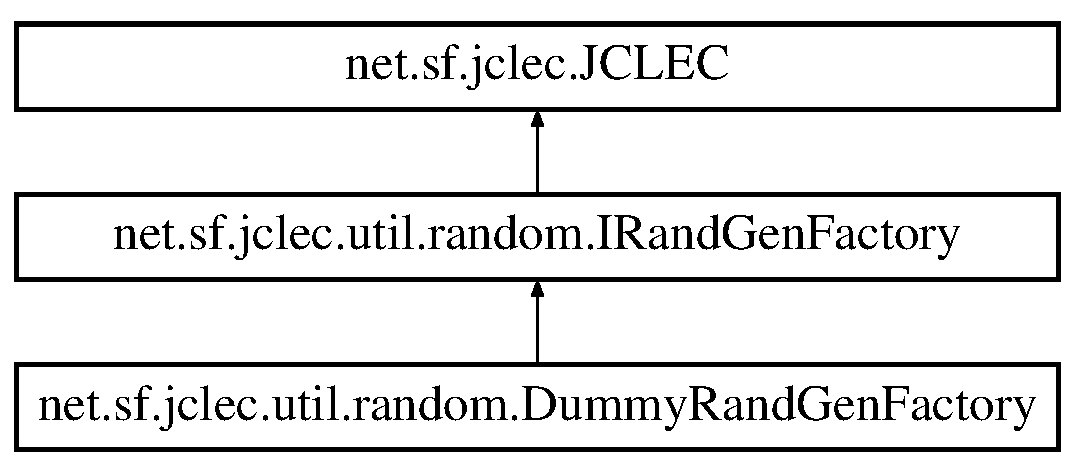
\includegraphics[height=2.000000cm]{classnet_1_1sf_1_1jclec_1_1util_1_1random_1_1_dummy_rand_gen_factory}
\end{center}
\end{figure}
\subsection*{Public Member Functions}
\begin{DoxyCompactItemize}
\item 
\hyperlink{interfacenet_1_1sf_1_1jclec_1_1util_1_1random_1_1_i_rand_gen}{I\-Rand\-Gen} \hyperlink{classnet_1_1sf_1_1jclec_1_1util_1_1random_1_1_dummy_rand_gen_factory_a3adb6be068a37e8ec08b9365f6417c85}{create\-Rand\-Gen} ()
\end{DoxyCompactItemize}


\subsection{Detailed Description}
\hyperlink{classnet_1_1sf_1_1jclec_1_1util_1_1random_1_1_dummy_rand_gen}{Dummy\-Rand\-Gen} factory.

\begin{DoxyAuthor}{Author}
Sebastian Ventura 
\end{DoxyAuthor}


\subsection{Member Function Documentation}
\hypertarget{classnet_1_1sf_1_1jclec_1_1util_1_1random_1_1_dummy_rand_gen_factory_a3adb6be068a37e8ec08b9365f6417c85}{\index{net\-::sf\-::jclec\-::util\-::random\-::\-Dummy\-Rand\-Gen\-Factory@{net\-::sf\-::jclec\-::util\-::random\-::\-Dummy\-Rand\-Gen\-Factory}!create\-Rand\-Gen@{create\-Rand\-Gen}}
\index{create\-Rand\-Gen@{create\-Rand\-Gen}!net::sf::jclec::util::random::DummyRandGenFactory@{net\-::sf\-::jclec\-::util\-::random\-::\-Dummy\-Rand\-Gen\-Factory}}
\subsubsection[{create\-Rand\-Gen}]{\setlength{\rightskip}{0pt plus 5cm}{\bf I\-Rand\-Gen} net.\-sf.\-jclec.\-util.\-random.\-Dummy\-Rand\-Gen\-Factory.\-create\-Rand\-Gen (
\begin{DoxyParamCaption}
{}
\end{DoxyParamCaption}
)}}\label{classnet_1_1sf_1_1jclec_1_1util_1_1random_1_1_dummy_rand_gen_factory_a3adb6be068a37e8ec08b9365f6417c85}
Factory method.

\begin{DoxyReturn}{Returns}
A new instance of a random generator 
\end{DoxyReturn}


Implements \hyperlink{interfacenet_1_1sf_1_1jclec_1_1util_1_1random_1_1_i_rand_gen_factory_a03320bb7d2eae4643d02ec66b08db1aa}{net.\-sf.\-jclec.\-util.\-random.\-I\-Rand\-Gen\-Factory}.



The documentation for this class was generated from the following file\-:\begin{DoxyCompactItemize}
\item 
src/test/java/net/sf/jclec/util/random/Dummy\-Rand\-Gen\-Factory.\-java\end{DoxyCompactItemize}

\hypertarget{classnet_1_1sf_1_1jclec_1_1realarray_1_1rec_1_1_einstein_connectives}{\section{net.\-sf.\-jclec.\-realarray.\-rec.\-Einstein\-Connectives Class Reference}
\label{classnet_1_1sf_1_1jclec_1_1realarray_1_1rec_1_1_einstein_connectives}\index{net.\-sf.\-jclec.\-realarray.\-rec.\-Einstein\-Connectives@{net.\-sf.\-jclec.\-realarray.\-rec.\-Einstein\-Connectives}}
}
Inheritance diagram for net.\-sf.\-jclec.\-realarray.\-rec.\-Einstein\-Connectives\-:\begin{figure}[H]
\begin{center}
\leavevmode
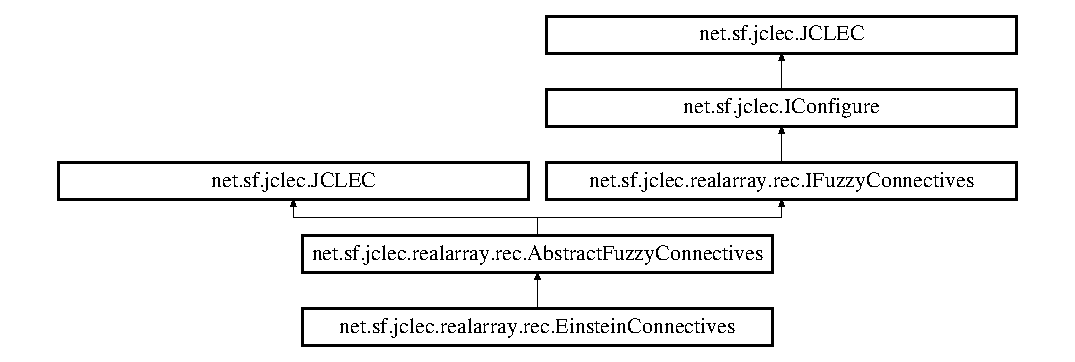
\includegraphics[height=4.416404cm]{classnet_1_1sf_1_1jclec_1_1realarray_1_1rec_1_1_einstein_connectives}
\end{center}
\end{figure}
\subsection*{Public Member Functions}
\begin{DoxyCompactItemize}
\item 
\hyperlink{classnet_1_1sf_1_1jclec_1_1realarray_1_1rec_1_1_einstein_connectives_a1cc72a5e21d70217dfd213eb9becc472}{Einstein\-Connectives} ()
\item 
double \hyperlink{classnet_1_1sf_1_1jclec_1_1realarray_1_1rec_1_1_einstein_connectives_a71258e1bc95be9f76c53eefb9e8b8d4b}{m} (double x, double y)
\item 
double \hyperlink{classnet_1_1sf_1_1jclec_1_1realarray_1_1rec_1_1_einstein_connectives_a478c20dfb3b17bc599ef1727dd55f8a0}{s} (double x, double y)
\item 
double \hyperlink{classnet_1_1sf_1_1jclec_1_1realarray_1_1rec_1_1_einstein_connectives_a00d986f392e8638f29ad3718dd67e0cc}{f} (double x, double y)
\item 
double \hyperlink{classnet_1_1sf_1_1jclec_1_1realarray_1_1rec_1_1_einstein_connectives_a9e0659d2327ad274e093181a133ad9ba}{l} (double x, double y)
\end{DoxyCompactItemize}


\subsection{Detailed Description}
Einstein Connectives.

\begin{DoxyAuthor}{Author}
Alberto Lamarca-\/\-Rosales 

Sebastian Ventura 
\end{DoxyAuthor}


\subsection{Constructor \& Destructor Documentation}
\hypertarget{classnet_1_1sf_1_1jclec_1_1realarray_1_1rec_1_1_einstein_connectives_a1cc72a5e21d70217dfd213eb9becc472}{\index{net\-::sf\-::jclec\-::realarray\-::rec\-::\-Einstein\-Connectives@{net\-::sf\-::jclec\-::realarray\-::rec\-::\-Einstein\-Connectives}!Einstein\-Connectives@{Einstein\-Connectives}}
\index{Einstein\-Connectives@{Einstein\-Connectives}!net::sf::jclec::realarray::rec::EinsteinConnectives@{net\-::sf\-::jclec\-::realarray\-::rec\-::\-Einstein\-Connectives}}
\subsubsection[{Einstein\-Connectives}]{\setlength{\rightskip}{0pt plus 5cm}net.\-sf.\-jclec.\-realarray.\-rec.\-Einstein\-Connectives.\-Einstein\-Connectives (
\begin{DoxyParamCaption}
{}
\end{DoxyParamCaption}
)}}\label{classnet_1_1sf_1_1jclec_1_1realarray_1_1rec_1_1_einstein_connectives_a1cc72a5e21d70217dfd213eb9becc472}
Empty constructor 

\subsection{Member Function Documentation}
\hypertarget{classnet_1_1sf_1_1jclec_1_1realarray_1_1rec_1_1_einstein_connectives_a00d986f392e8638f29ad3718dd67e0cc}{\index{net\-::sf\-::jclec\-::realarray\-::rec\-::\-Einstein\-Connectives@{net\-::sf\-::jclec\-::realarray\-::rec\-::\-Einstein\-Connectives}!f@{f}}
\index{f@{f}!net::sf::jclec::realarray::rec::EinsteinConnectives@{net\-::sf\-::jclec\-::realarray\-::rec\-::\-Einstein\-Connectives}}
\subsubsection[{f}]{\setlength{\rightskip}{0pt plus 5cm}double net.\-sf.\-jclec.\-realarray.\-rec.\-Einstein\-Connectives.\-f (
\begin{DoxyParamCaption}
\item[{double}]{x, }
\item[{double}]{y}
\end{DoxyParamCaption}
)\hspace{0.3cm}{\ttfamily [virtual]}}}\label{classnet_1_1sf_1_1jclec_1_1realarray_1_1rec_1_1_einstein_connectives_a00d986f392e8638f29ad3718dd67e0cc}
Einstein Function f 

Implements \hyperlink{interfacenet_1_1sf_1_1jclec_1_1realarray_1_1rec_1_1_i_fuzzy_connectives_a970200edf4d66083e0ad040096783c35}{net.\-sf.\-jclec.\-realarray.\-rec.\-I\-Fuzzy\-Connectives}.

\hypertarget{classnet_1_1sf_1_1jclec_1_1realarray_1_1rec_1_1_einstein_connectives_a9e0659d2327ad274e093181a133ad9ba}{\index{net\-::sf\-::jclec\-::realarray\-::rec\-::\-Einstein\-Connectives@{net\-::sf\-::jclec\-::realarray\-::rec\-::\-Einstein\-Connectives}!l@{l}}
\index{l@{l}!net::sf::jclec::realarray::rec::EinsteinConnectives@{net\-::sf\-::jclec\-::realarray\-::rec\-::\-Einstein\-Connectives}}
\subsubsection[{l}]{\setlength{\rightskip}{0pt plus 5cm}double net.\-sf.\-jclec.\-realarray.\-rec.\-Einstein\-Connectives.\-l (
\begin{DoxyParamCaption}
\item[{double}]{x, }
\item[{double}]{y}
\end{DoxyParamCaption}
)\hspace{0.3cm}{\ttfamily [virtual]}}}\label{classnet_1_1sf_1_1jclec_1_1realarray_1_1rec_1_1_einstein_connectives_a9e0659d2327ad274e093181a133ad9ba}
Einstein Function l 

Implements \hyperlink{interfacenet_1_1sf_1_1jclec_1_1realarray_1_1rec_1_1_i_fuzzy_connectives_a0cea5560723101682211330bba9e20e4}{net.\-sf.\-jclec.\-realarray.\-rec.\-I\-Fuzzy\-Connectives}.

\hypertarget{classnet_1_1sf_1_1jclec_1_1realarray_1_1rec_1_1_einstein_connectives_a71258e1bc95be9f76c53eefb9e8b8d4b}{\index{net\-::sf\-::jclec\-::realarray\-::rec\-::\-Einstein\-Connectives@{net\-::sf\-::jclec\-::realarray\-::rec\-::\-Einstein\-Connectives}!m@{m}}
\index{m@{m}!net::sf::jclec::realarray::rec::EinsteinConnectives@{net\-::sf\-::jclec\-::realarray\-::rec\-::\-Einstein\-Connectives}}
\subsubsection[{m}]{\setlength{\rightskip}{0pt plus 5cm}double net.\-sf.\-jclec.\-realarray.\-rec.\-Einstein\-Connectives.\-m (
\begin{DoxyParamCaption}
\item[{double}]{x, }
\item[{double}]{y}
\end{DoxyParamCaption}
)\hspace{0.3cm}{\ttfamily [virtual]}}}\label{classnet_1_1sf_1_1jclec_1_1realarray_1_1rec_1_1_einstein_connectives_a71258e1bc95be9f76c53eefb9e8b8d4b}
Einstein Function m 

Implements \hyperlink{interfacenet_1_1sf_1_1jclec_1_1realarray_1_1rec_1_1_i_fuzzy_connectives_acd07fed683410b0147e04075b8d6aea6}{net.\-sf.\-jclec.\-realarray.\-rec.\-I\-Fuzzy\-Connectives}.

\hypertarget{classnet_1_1sf_1_1jclec_1_1realarray_1_1rec_1_1_einstein_connectives_a478c20dfb3b17bc599ef1727dd55f8a0}{\index{net\-::sf\-::jclec\-::realarray\-::rec\-::\-Einstein\-Connectives@{net\-::sf\-::jclec\-::realarray\-::rec\-::\-Einstein\-Connectives}!s@{s}}
\index{s@{s}!net::sf::jclec::realarray::rec::EinsteinConnectives@{net\-::sf\-::jclec\-::realarray\-::rec\-::\-Einstein\-Connectives}}
\subsubsection[{s}]{\setlength{\rightskip}{0pt plus 5cm}double net.\-sf.\-jclec.\-realarray.\-rec.\-Einstein\-Connectives.\-s (
\begin{DoxyParamCaption}
\item[{double}]{x, }
\item[{double}]{y}
\end{DoxyParamCaption}
)\hspace{0.3cm}{\ttfamily [virtual]}}}\label{classnet_1_1sf_1_1jclec_1_1realarray_1_1rec_1_1_einstein_connectives_a478c20dfb3b17bc599ef1727dd55f8a0}
Einstein Function s 

Implements \hyperlink{interfacenet_1_1sf_1_1jclec_1_1realarray_1_1rec_1_1_i_fuzzy_connectives_a2ae764e485434e088a8128a9e2bea734}{net.\-sf.\-jclec.\-realarray.\-rec.\-I\-Fuzzy\-Connectives}.



The documentation for this class was generated from the following file\-:\begin{DoxyCompactItemize}
\item 
src/main/java/net/sf/jclec/realarray/rec/Einstein\-Connectives.\-java\end{DoxyCompactItemize}

\hypertarget{classnet_1_1sf_1_1jclec_1_1realarray_1_1_euclidean_distance}{\section{net.\-sf.\-jclec.\-realarray.\-Euclidean\-Distance Class Reference}
\label{classnet_1_1sf_1_1jclec_1_1realarray_1_1_euclidean_distance}\index{net.\-sf.\-jclec.\-realarray.\-Euclidean\-Distance@{net.\-sf.\-jclec.\-realarray.\-Euclidean\-Distance}}
}
Inheritance diagram for net.\-sf.\-jclec.\-realarray.\-Euclidean\-Distance\-:\begin{figure}[H]
\begin{center}
\leavevmode
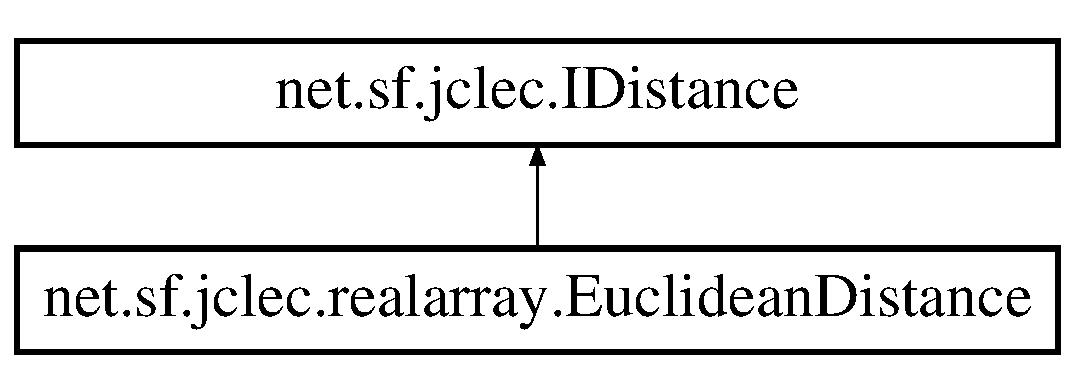
\includegraphics[height=2.000000cm]{classnet_1_1sf_1_1jclec_1_1realarray_1_1_euclidean_distance}
\end{center}
\end{figure}
\subsection*{Public Member Functions}
\begin{DoxyCompactItemize}
\item 
\hyperlink{classnet_1_1sf_1_1jclec_1_1realarray_1_1_euclidean_distance_af284caee3ce51b7b0e180100639c323d}{Euclidean\-Distance} ()
\item 
double \hyperlink{classnet_1_1sf_1_1jclec_1_1realarray_1_1_euclidean_distance_ace3d61ddf5512cb35d3d3a635e8e203e}{distance} (\hyperlink{interfacenet_1_1sf_1_1jclec_1_1_i_individual}{I\-Individual} one, \hyperlink{interfacenet_1_1sf_1_1jclec_1_1_i_individual}{I\-Individual} other)
\end{DoxyCompactItemize}


\subsection{Detailed Description}
Euclidean distance

\begin{DoxyAuthor}{Author}
Sebastian Ventura 
\end{DoxyAuthor}


\subsection{Constructor \& Destructor Documentation}
\hypertarget{classnet_1_1sf_1_1jclec_1_1realarray_1_1_euclidean_distance_af284caee3ce51b7b0e180100639c323d}{\index{net\-::sf\-::jclec\-::realarray\-::\-Euclidean\-Distance@{net\-::sf\-::jclec\-::realarray\-::\-Euclidean\-Distance}!Euclidean\-Distance@{Euclidean\-Distance}}
\index{Euclidean\-Distance@{Euclidean\-Distance}!net::sf::jclec::realarray::EuclideanDistance@{net\-::sf\-::jclec\-::realarray\-::\-Euclidean\-Distance}}
\subsubsection[{Euclidean\-Distance}]{\setlength{\rightskip}{0pt plus 5cm}net.\-sf.\-jclec.\-realarray.\-Euclidean\-Distance.\-Euclidean\-Distance (
\begin{DoxyParamCaption}
{}
\end{DoxyParamCaption}
)}}\label{classnet_1_1sf_1_1jclec_1_1realarray_1_1_euclidean_distance_af284caee3ce51b7b0e180100639c323d}
Empty (default) constructor 

\subsection{Member Function Documentation}
\hypertarget{classnet_1_1sf_1_1jclec_1_1realarray_1_1_euclidean_distance_ace3d61ddf5512cb35d3d3a635e8e203e}{\index{net\-::sf\-::jclec\-::realarray\-::\-Euclidean\-Distance@{net\-::sf\-::jclec\-::realarray\-::\-Euclidean\-Distance}!distance@{distance}}
\index{distance@{distance}!net::sf::jclec::realarray::EuclideanDistance@{net\-::sf\-::jclec\-::realarray\-::\-Euclidean\-Distance}}
\subsubsection[{distance}]{\setlength{\rightskip}{0pt plus 5cm}double net.\-sf.\-jclec.\-realarray.\-Euclidean\-Distance.\-distance (
\begin{DoxyParamCaption}
\item[{{\bf I\-Individual}}]{one, }
\item[{{\bf I\-Individual}}]{other}
\end{DoxyParamCaption}
)\hspace{0.3cm}{\ttfamily [virtual]}}}\label{classnet_1_1sf_1_1jclec_1_1realarray_1_1_euclidean_distance_ace3d61ddf5512cb35d3d3a635e8e203e}
Distance method.


\begin{DoxyParams}{Parameters}
{\em one} & First individual to compare \\
\hline
{\em other} & Second individual to compare\\
\hline
\end{DoxyParams}
\begin{DoxyReturn}{Returns}
Distance between individuals {\ttfamily one} and {\ttfamily other}
\end{DoxyReturn}
 

Implements \hyperlink{interfacenet_1_1sf_1_1jclec_1_1_i_distance_a6f0220da1f5f7926f0ecc15c30b8a7d6}{net.\-sf.\-jclec.\-I\-Distance}.



The documentation for this class was generated from the following file\-:\begin{DoxyCompactItemize}
\item 
src/main/java/net/sf/jclec/realarray/Euclidean\-Distance.\-java\end{DoxyCompactItemize}

\hypertarget{classnet_1_1sf_1_1jclec_1_1exprtree_1_1fun_1_1_execute_expr_tree_function}{\section{net.\-sf.\-jclec.\-exprtree.\-fun.\-Execute\-Expr\-Tree\-Function Class Reference}
\label{classnet_1_1sf_1_1jclec_1_1exprtree_1_1fun_1_1_execute_expr_tree_function}\index{net.\-sf.\-jclec.\-exprtree.\-fun.\-Execute\-Expr\-Tree\-Function@{net.\-sf.\-jclec.\-exprtree.\-fun.\-Execute\-Expr\-Tree\-Function}}
}
\subsection*{Static Public Member Functions}
\begin{DoxyCompactItemize}
\item 
static void \hyperlink{classnet_1_1sf_1_1jclec_1_1exprtree_1_1fun_1_1_execute_expr_tree_function_a78ff449a442d9c3799307196201a612c}{main} (String\mbox{[}$\,$\mbox{]} args)
\end{DoxyCompactItemize}


\subsection{Detailed Description}
\hyperlink{classnet_1_1sf_1_1jclec_1_1exprtree_1_1fun_1_1_expr_tree_function}{Expr\-Tree\-Function} execution example

\begin{DoxyAuthor}{Author}
Sebastian Ventura 
\end{DoxyAuthor}


\subsection{Member Function Documentation}
\hypertarget{classnet_1_1sf_1_1jclec_1_1exprtree_1_1fun_1_1_execute_expr_tree_function_a78ff449a442d9c3799307196201a612c}{\index{net\-::sf\-::jclec\-::exprtree\-::fun\-::\-Execute\-Expr\-Tree\-Function@{net\-::sf\-::jclec\-::exprtree\-::fun\-::\-Execute\-Expr\-Tree\-Function}!main@{main}}
\index{main@{main}!net::sf::jclec::exprtree::fun::ExecuteExprTreeFunction@{net\-::sf\-::jclec\-::exprtree\-::fun\-::\-Execute\-Expr\-Tree\-Function}}
\subsubsection[{main}]{\setlength{\rightskip}{0pt plus 5cm}static void net.\-sf.\-jclec.\-exprtree.\-fun.\-Execute\-Expr\-Tree\-Function.\-main (
\begin{DoxyParamCaption}
\item[{String\mbox{[}$\,$\mbox{]}}]{args}
\end{DoxyParamCaption}
)\hspace{0.3cm}{\ttfamily [static]}}}\label{classnet_1_1sf_1_1jclec_1_1exprtree_1_1fun_1_1_execute_expr_tree_function_a78ff449a442d9c3799307196201a612c}
This method perform the following steps\-:


\begin{DoxyItemize}
\item Create an \hyperlink{classnet_1_1sf_1_1jclec_1_1exprtree_1_1_expr_tree}{Expr\-Tree} object 
\item Add several nodes (primitives) to this expression tree 
\item Create an \hyperlink{classnet_1_1sf_1_1jclec_1_1exprtree_1_1fun_1_1_expr_tree_function}{Expr\-Tree\-Function} object 
\item Assign \hyperlink{classnet_1_1sf_1_1jclec_1_1exprtree_1_1_expr_tree}{Expr\-Tree} object as funtion code 
\item Execute function 
\end{DoxyItemize}

The documentation for this class was generated from the following file\-:\begin{DoxyCompactItemize}
\item 
src/test/java/net/sf/jclec/exprtree/fun/Execute\-Expr\-Tree\-Function.\-java\end{DoxyCompactItemize}

\hypertarget{classnet_1_1sf_1_1jclec_1_1syntaxtree_1_1mut_1_1_expand_n_t_mutator}{\section{net.\-sf.\-jclec.\-syntaxtree.\-mut.\-Expand\-N\-T\-Mutator Class Reference}
\label{classnet_1_1sf_1_1jclec_1_1syntaxtree_1_1mut_1_1_expand_n_t_mutator}\index{net.\-sf.\-jclec.\-syntaxtree.\-mut.\-Expand\-N\-T\-Mutator@{net.\-sf.\-jclec.\-syntaxtree.\-mut.\-Expand\-N\-T\-Mutator}}
}
Inheritance diagram for net.\-sf.\-jclec.\-syntaxtree.\-mut.\-Expand\-N\-T\-Mutator\-:\begin{figure}[H]
\begin{center}
\leavevmode
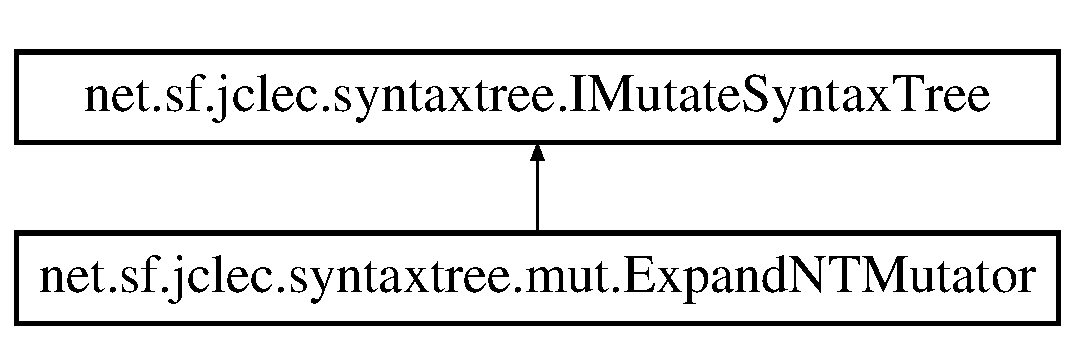
\includegraphics[height=2.000000cm]{classnet_1_1sf_1_1jclec_1_1syntaxtree_1_1mut_1_1_expand_n_t_mutator}
\end{center}
\end{figure}
\subsection*{Public Member Functions}
\begin{DoxyCompactItemize}
\item 
\hyperlink{classnet_1_1sf_1_1jclec_1_1syntaxtree_1_1mut_1_1_expand_n_t_mutator_a726057809fe6521937788448b41a80ae}{Expand\-N\-T\-Mutator} ()
\item 
\hyperlink{classnet_1_1sf_1_1jclec_1_1syntaxtree_1_1_syntax_tree}{Syntax\-Tree} \hyperlink{classnet_1_1sf_1_1jclec_1_1syntaxtree_1_1mut_1_1_expand_n_t_mutator_a1d141078f04df8fe00572b0dd6f484ed}{mutate\-Syntax\-Tree} (\hyperlink{classnet_1_1sf_1_1jclec_1_1syntaxtree_1_1_syntax_tree}{Syntax\-Tree} parent, \hyperlink{classnet_1_1sf_1_1jclec_1_1syntaxtree_1_1_syntax_tree_schema}{Syntax\-Tree\-Schema} schema, \hyperlink{interfacenet_1_1sf_1_1jclec_1_1util_1_1random_1_1_i_rand_gen}{I\-Rand\-Gen} randgen)
\end{DoxyCompactItemize}


\subsection{Detailed Description}
Expand\-N\-T mutator.

Realiza una exploracion del espacio de busqueda de forma incremental, incrementando en cada paso la profundidad de los arboles mediante la modificacion aleatoria de una rama del arbol.

\begin{DoxyAuthor}{Author}
Amelia Zafra 
\end{DoxyAuthor}


\subsection{Constructor \& Destructor Documentation}
\hypertarget{classnet_1_1sf_1_1jclec_1_1syntaxtree_1_1mut_1_1_expand_n_t_mutator_a726057809fe6521937788448b41a80ae}{\index{net\-::sf\-::jclec\-::syntaxtree\-::mut\-::\-Expand\-N\-T\-Mutator@{net\-::sf\-::jclec\-::syntaxtree\-::mut\-::\-Expand\-N\-T\-Mutator}!Expand\-N\-T\-Mutator@{Expand\-N\-T\-Mutator}}
\index{Expand\-N\-T\-Mutator@{Expand\-N\-T\-Mutator}!net::sf::jclec::syntaxtree::mut::ExpandNTMutator@{net\-::sf\-::jclec\-::syntaxtree\-::mut\-::\-Expand\-N\-T\-Mutator}}
\subsubsection[{Expand\-N\-T\-Mutator}]{\setlength{\rightskip}{0pt plus 5cm}net.\-sf.\-jclec.\-syntaxtree.\-mut.\-Expand\-N\-T\-Mutator.\-Expand\-N\-T\-Mutator (
\begin{DoxyParamCaption}
{}
\end{DoxyParamCaption}
)}}\label{classnet_1_1sf_1_1jclec_1_1syntaxtree_1_1mut_1_1_expand_n_t_mutator_a726057809fe6521937788448b41a80ae}
Empty constructor 

\subsection{Member Function Documentation}
\hypertarget{classnet_1_1sf_1_1jclec_1_1syntaxtree_1_1mut_1_1_expand_n_t_mutator_a1d141078f04df8fe00572b0dd6f484ed}{\index{net\-::sf\-::jclec\-::syntaxtree\-::mut\-::\-Expand\-N\-T\-Mutator@{net\-::sf\-::jclec\-::syntaxtree\-::mut\-::\-Expand\-N\-T\-Mutator}!mutate\-Syntax\-Tree@{mutate\-Syntax\-Tree}}
\index{mutate\-Syntax\-Tree@{mutate\-Syntax\-Tree}!net::sf::jclec::syntaxtree::mut::ExpandNTMutator@{net\-::sf\-::jclec\-::syntaxtree\-::mut\-::\-Expand\-N\-T\-Mutator}}
\subsubsection[{mutate\-Syntax\-Tree}]{\setlength{\rightskip}{0pt plus 5cm}{\bf Syntax\-Tree} net.\-sf.\-jclec.\-syntaxtree.\-mut.\-Expand\-N\-T\-Mutator.\-mutate\-Syntax\-Tree (
\begin{DoxyParamCaption}
\item[{{\bf Syntax\-Tree}}]{tree, }
\item[{{\bf Syntax\-Tree\-Schema}}]{tree\-Schema, }
\item[{{\bf I\-Rand\-Gen}}]{randgen}
\end{DoxyParamCaption}
)\hspace{0.3cm}{\ttfamily [virtual]}}}\label{classnet_1_1sf_1_1jclec_1_1syntaxtree_1_1mut_1_1_expand_n_t_mutator_a1d141078f04df8fe00572b0dd6f484ed}

\begin{DoxyParams}{Parameters}
{\em tree} & \\
\hline
{\em tree\-Schema} & \\
\hline
{\em randgen} & \\
\hline
\end{DoxyParams}
\begin{DoxyReturn}{Returns}
A new expression tree 
\end{DoxyReturn}


Implements \hyperlink{interfacenet_1_1sf_1_1jclec_1_1syntaxtree_1_1_i_mutate_syntax_tree_ac458c63a51084cb0614e5afc5e523625}{net.\-sf.\-jclec.\-syntaxtree.\-I\-Mutate\-Syntax\-Tree}.



The documentation for this class was generated from the following file\-:\begin{DoxyCompactItemize}
\item 
src/main/java/net/sf/jclec/syntaxtree/mut/Expand\-N\-T\-Mutator.\-java\end{DoxyCompactItemize}

\hypertarget{classnet_1_1sf_1_1jclec_1_1syntaxtree_1_1mut_1_1_expand_n_t_mutator_test}{\section{net.\-sf.\-jclec.\-syntaxtree.\-mut.\-Expand\-N\-T\-Mutator\-Test Class Reference}
\label{classnet_1_1sf_1_1jclec_1_1syntaxtree_1_1mut_1_1_expand_n_t_mutator_test}\index{net.\-sf.\-jclec.\-syntaxtree.\-mut.\-Expand\-N\-T\-Mutator\-Test@{net.\-sf.\-jclec.\-syntaxtree.\-mut.\-Expand\-N\-T\-Mutator\-Test}}
}
Inheritance diagram for net.\-sf.\-jclec.\-syntaxtree.\-mut.\-Expand\-N\-T\-Mutator\-Test\-:\begin{figure}[H]
\begin{center}
\leavevmode
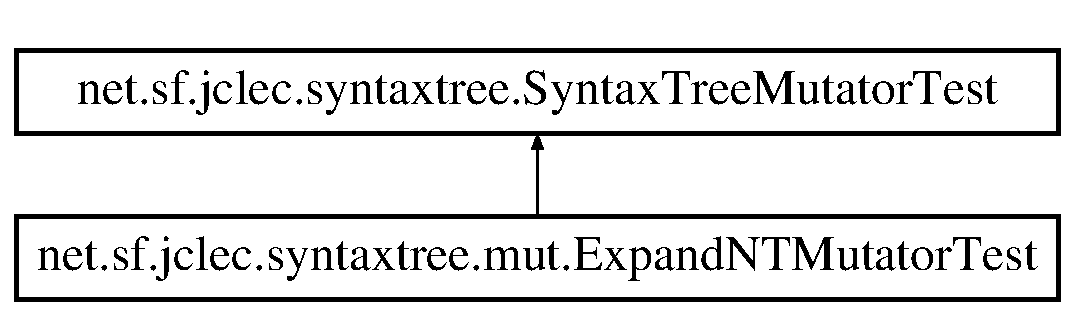
\includegraphics[height=2.000000cm]{classnet_1_1sf_1_1jclec_1_1syntaxtree_1_1mut_1_1_expand_n_t_mutator_test}
\end{center}
\end{figure}
\subsection*{Public Member Functions}
\begin{DoxyCompactItemize}
\item 
\hyperlink{classnet_1_1sf_1_1jclec_1_1syntaxtree_1_1mut_1_1_expand_n_t_mutator_test_a6615ff0e064ec04c1ac729016ca5531b}{Expand\-N\-T\-Mutator\-Test} (String name)
\end{DoxyCompactItemize}


\subsection{Detailed Description}
Unit tests for \hyperlink{classnet_1_1sf_1_1jclec_1_1syntaxtree_1_1mut_1_1_expand_n_t_mutator_test}{Expand\-N\-T\-Mutator\-Test}.

\begin{DoxyAuthor}{Author}
Amelia Zafra 

Sebastian Ventura 
\end{DoxyAuthor}


\subsection{Constructor \& Destructor Documentation}
\hypertarget{classnet_1_1sf_1_1jclec_1_1syntaxtree_1_1mut_1_1_expand_n_t_mutator_test_a6615ff0e064ec04c1ac729016ca5531b}{\index{net\-::sf\-::jclec\-::syntaxtree\-::mut\-::\-Expand\-N\-T\-Mutator\-Test@{net\-::sf\-::jclec\-::syntaxtree\-::mut\-::\-Expand\-N\-T\-Mutator\-Test}!Expand\-N\-T\-Mutator\-Test@{Expand\-N\-T\-Mutator\-Test}}
\index{Expand\-N\-T\-Mutator\-Test@{Expand\-N\-T\-Mutator\-Test}!net::sf::jclec::syntaxtree::mut::ExpandNTMutatorTest@{net\-::sf\-::jclec\-::syntaxtree\-::mut\-::\-Expand\-N\-T\-Mutator\-Test}}
\subsubsection[{Expand\-N\-T\-Mutator\-Test}]{\setlength{\rightskip}{0pt plus 5cm}net.\-sf.\-jclec.\-syntaxtree.\-mut.\-Expand\-N\-T\-Mutator\-Test.\-Expand\-N\-T\-Mutator\-Test (
\begin{DoxyParamCaption}
\item[{String}]{name}
\end{DoxyParamCaption}
)}}\label{classnet_1_1sf_1_1jclec_1_1syntaxtree_1_1mut_1_1_expand_n_t_mutator_test_a6615ff0e064ec04c1ac729016ca5531b}
Default constructor. 

The documentation for this class was generated from the following file\-:\begin{DoxyCompactItemize}
\item 
src/test/java/net/sf/jclec/syntaxtree/mut/Expand\-N\-T\-Mutator\-Test.\-java\end{DoxyCompactItemize}

\hypertarget{classnet_1_1sf_1_1jclec_1_1_experiment_builder}{\section{net.\-sf.\-jclec.\-Experiment\-Builder Class Reference}
\label{classnet_1_1sf_1_1jclec_1_1_experiment_builder}\index{net.\-sf.\-jclec.\-Experiment\-Builder@{net.\-sf.\-jclec.\-Experiment\-Builder}}
}
\subsection*{Public Member Functions}
\begin{DoxyCompactItemize}
\item 
\hyperlink{classnet_1_1sf_1_1jclec_1_1_experiment_builder_ae2aeacc6fb353d0380d5e81365a89635}{Experiment\-Builder} ()
\item 
Array\-List$<$ String $>$ \hyperlink{classnet_1_1sf_1_1jclec_1_1_experiment_builder_a087d2fb2f4e12352db1b661e9a2c925f}{build\-Experiment} (String experiment\-File\-Name)
\end{DoxyCompactItemize}


\subsection{Detailed Description}
Experiments builder

\begin{DoxyAuthor}{Author}
Sebastian Ventura 

Jose M. Luna 

Alberto Cano 

Juan Luis Olmo 

Amelia Zafra 
\end{DoxyAuthor}


\subsection{Constructor \& Destructor Documentation}
\hypertarget{classnet_1_1sf_1_1jclec_1_1_experiment_builder_ae2aeacc6fb353d0380d5e81365a89635}{\index{net\-::sf\-::jclec\-::\-Experiment\-Builder@{net\-::sf\-::jclec\-::\-Experiment\-Builder}!Experiment\-Builder@{Experiment\-Builder}}
\index{Experiment\-Builder@{Experiment\-Builder}!net::sf::jclec::ExperimentBuilder@{net\-::sf\-::jclec\-::\-Experiment\-Builder}}
\subsubsection[{Experiment\-Builder}]{\setlength{\rightskip}{0pt plus 5cm}net.\-sf.\-jclec.\-Experiment\-Builder.\-Experiment\-Builder (
\begin{DoxyParamCaption}
{}
\end{DoxyParamCaption}
)}}\label{classnet_1_1sf_1_1jclec_1_1_experiment_builder_ae2aeacc6fb353d0380d5e81365a89635}
Empty constructor 

\subsection{Member Function Documentation}
\hypertarget{classnet_1_1sf_1_1jclec_1_1_experiment_builder_a087d2fb2f4e12352db1b661e9a2c925f}{\index{net\-::sf\-::jclec\-::\-Experiment\-Builder@{net\-::sf\-::jclec\-::\-Experiment\-Builder}!build\-Experiment@{build\-Experiment}}
\index{build\-Experiment@{build\-Experiment}!net::sf::jclec::ExperimentBuilder@{net\-::sf\-::jclec\-::\-Experiment\-Builder}}
\subsubsection[{build\-Experiment}]{\setlength{\rightskip}{0pt plus 5cm}Array\-List$<$String$>$ net.\-sf.\-jclec.\-Experiment\-Builder.\-build\-Experiment (
\begin{DoxyParamCaption}
\item[{String}]{experiment\-File\-Name}
\end{DoxyParamCaption}
)}}\label{classnet_1_1sf_1_1jclec_1_1_experiment_builder_a087d2fb2f4e12352db1b661e9a2c925f}
Expands the experiments for the configuration file Expand multi-\/valued elements

Expand multi-\/valued attributes

Remove temp files

Move the expanded configuration files to the experiments folder

If the directory exists, delete all files

Else, create the directory

Return the configuration filenames 

The documentation for this class was generated from the following file\-:\begin{DoxyCompactItemize}
\item 
src/main/java/net/sf/jclec/Experiment\-Builder.\-java\end{DoxyCompactItemize}

\hypertarget{classnet_1_1sf_1_1jclec_1_1exprtree_1_1_expr_tree}{\section{net.\-sf.\-jclec.\-exprtree.\-Expr\-Tree Class Reference}
\label{classnet_1_1sf_1_1jclec_1_1exprtree_1_1_expr_tree}\index{net.\-sf.\-jclec.\-exprtree.\-Expr\-Tree@{net.\-sf.\-jclec.\-exprtree.\-Expr\-Tree}}
}


Inherits net.\-sf.\-jclec.\-J\-C\-L\-E\-C.

\subsection*{Public Member Functions}
\begin{DoxyCompactItemize}
\item 
\hyperlink{classnet_1_1sf_1_1jclec_1_1exprtree_1_1_expr_tree_a85c2c8dfa902edb3aa5072222b990bda}{Expr\-Tree} ()
\item 
void \hyperlink{classnet_1_1sf_1_1jclec_1_1exprtree_1_1_expr_tree_afe0d2782c07ec7535af397f988e498cf}{add\-Block} (\hyperlink{interfacenet_1_1sf_1_1jclec_1_1exprtree_1_1_i_primitive}{I\-Primitive} block)
\item 
\hyperlink{interfacenet_1_1sf_1_1jclec_1_1exprtree_1_1_i_primitive}{I\-Primitive} \hyperlink{classnet_1_1sf_1_1jclec_1_1exprtree_1_1_expr_tree_a1dce5503763804028585f66df548fb57}{get\-Block} (int block\-Index)
\item 
void \hyperlink{classnet_1_1sf_1_1jclec_1_1exprtree_1_1_expr_tree_af746344b2364363781a393238e6ec81a}{set\-Block} (\hyperlink{interfacenet_1_1sf_1_1jclec_1_1exprtree_1_1_i_primitive}{I\-Primitive} block, int block\-Index)
\item 
int \hyperlink{classnet_1_1sf_1_1jclec_1_1exprtree_1_1_expr_tree_ace3e27d755f5eb9f8085f418f17b8bf4}{size} ()
\item 
\hyperlink{classnet_1_1sf_1_1jclec_1_1exprtree_1_1_expr_tree}{Expr\-Tree} \hyperlink{classnet_1_1sf_1_1jclec_1_1exprtree_1_1_expr_tree_aa045415684bf4b6561c4f9181a5bd51c}{copy} ()
\item 
int \hyperlink{classnet_1_1sf_1_1jclec_1_1exprtree_1_1_expr_tree_a382dcb6253aa6413996360a4f06f112f}{sub\-Tree} (int root\-Index)
\item 
Iterator$<$ \hyperlink{interfacenet_1_1sf_1_1jclec_1_1exprtree_1_1_i_primitive}{I\-Primitive} $>$ \hyperlink{classnet_1_1sf_1_1jclec_1_1exprtree_1_1_expr_tree_a217aa20e10a46a89e0a1a1d5d12abd63}{execute\-Iterator} ()
\item 
String \hyperlink{classnet_1_1sf_1_1jclec_1_1exprtree_1_1_expr_tree_a4123b9cc1de989e37815c1d229b00528}{to\-String} ()
\item 
boolean \hyperlink{classnet_1_1sf_1_1jclec_1_1exprtree_1_1_expr_tree_ac3efbfd612ef016a6a028f426530ea53}{equals} (Object other)
\end{DoxyCompactItemize}


\subsection{Detailed Description}
Expression tree.

\begin{DoxyAuthor}{Author}
Sebastian Ventura 
\end{DoxyAuthor}


\subsection{Constructor \& Destructor Documentation}
\hypertarget{classnet_1_1sf_1_1jclec_1_1exprtree_1_1_expr_tree_a85c2c8dfa902edb3aa5072222b990bda}{\index{net\-::sf\-::jclec\-::exprtree\-::\-Expr\-Tree@{net\-::sf\-::jclec\-::exprtree\-::\-Expr\-Tree}!Expr\-Tree@{Expr\-Tree}}
\index{Expr\-Tree@{Expr\-Tree}!net::sf::jclec::exprtree::ExprTree@{net\-::sf\-::jclec\-::exprtree\-::\-Expr\-Tree}}
\subsubsection[{Expr\-Tree}]{\setlength{\rightskip}{0pt plus 5cm}net.\-sf.\-jclec.\-exprtree.\-Expr\-Tree.\-Expr\-Tree (
\begin{DoxyParamCaption}
{}
\end{DoxyParamCaption}
)}}\label{classnet_1_1sf_1_1jclec_1_1exprtree_1_1_expr_tree_a85c2c8dfa902edb3aa5072222b990bda}
Constructor 

\subsection{Member Function Documentation}
\hypertarget{classnet_1_1sf_1_1jclec_1_1exprtree_1_1_expr_tree_afe0d2782c07ec7535af397f988e498cf}{\index{net\-::sf\-::jclec\-::exprtree\-::\-Expr\-Tree@{net\-::sf\-::jclec\-::exprtree\-::\-Expr\-Tree}!add\-Block@{add\-Block}}
\index{add\-Block@{add\-Block}!net::sf::jclec::exprtree::ExprTree@{net\-::sf\-::jclec\-::exprtree\-::\-Expr\-Tree}}
\subsubsection[{add\-Block}]{\setlength{\rightskip}{0pt plus 5cm}void net.\-sf.\-jclec.\-exprtree.\-Expr\-Tree.\-add\-Block (
\begin{DoxyParamCaption}
\item[{{\bf I\-Primitive}}]{block}
\end{DoxyParamCaption}
)}}\label{classnet_1_1sf_1_1jclec_1_1exprtree_1_1_expr_tree_afe0d2782c07ec7535af397f988e498cf}
Add a block to this expression.


\begin{DoxyParams}{Parameters}
{\em block} & Block to add \\
\hline
\end{DoxyParams}
\hypertarget{classnet_1_1sf_1_1jclec_1_1exprtree_1_1_expr_tree_aa045415684bf4b6561c4f9181a5bd51c}{\index{net\-::sf\-::jclec\-::exprtree\-::\-Expr\-Tree@{net\-::sf\-::jclec\-::exprtree\-::\-Expr\-Tree}!copy@{copy}}
\index{copy@{copy}!net::sf::jclec::exprtree::ExprTree@{net\-::sf\-::jclec\-::exprtree\-::\-Expr\-Tree}}
\subsubsection[{copy}]{\setlength{\rightskip}{0pt plus 5cm}{\bf Expr\-Tree} net.\-sf.\-jclec.\-exprtree.\-Expr\-Tree.\-copy (
\begin{DoxyParamCaption}
{}
\end{DoxyParamCaption}
)}}\label{classnet_1_1sf_1_1jclec_1_1exprtree_1_1_expr_tree_aa045415684bf4b6561c4f9181a5bd51c}
Copy method.

\begin{DoxyReturn}{Returns}
A copy of this expression tree 
\end{DoxyReturn}
\hypertarget{classnet_1_1sf_1_1jclec_1_1exprtree_1_1_expr_tree_ac3efbfd612ef016a6a028f426530ea53}{\index{net\-::sf\-::jclec\-::exprtree\-::\-Expr\-Tree@{net\-::sf\-::jclec\-::exprtree\-::\-Expr\-Tree}!equals@{equals}}
\index{equals@{equals}!net::sf::jclec::exprtree::ExprTree@{net\-::sf\-::jclec\-::exprtree\-::\-Expr\-Tree}}
\subsubsection[{equals}]{\setlength{\rightskip}{0pt plus 5cm}boolean net.\-sf.\-jclec.\-exprtree.\-Expr\-Tree.\-equals (
\begin{DoxyParamCaption}
\item[{Object}]{other}
\end{DoxyParamCaption}
)}}\label{classnet_1_1sf_1_1jclec_1_1exprtree_1_1_expr_tree_ac3efbfd612ef016a6a028f426530ea53}
\hypertarget{classnet_1_1sf_1_1jclec_1_1exprtree_1_1_expr_tree_a217aa20e10a46a89e0a1a1d5d12abd63}{\index{net\-::sf\-::jclec\-::exprtree\-::\-Expr\-Tree@{net\-::sf\-::jclec\-::exprtree\-::\-Expr\-Tree}!execute\-Iterator@{execute\-Iterator}}
\index{execute\-Iterator@{execute\-Iterator}!net::sf::jclec::exprtree::ExprTree@{net\-::sf\-::jclec\-::exprtree\-::\-Expr\-Tree}}
\subsubsection[{execute\-Iterator}]{\setlength{\rightskip}{0pt plus 5cm}Iterator$<${\bf I\-Primitive}$>$ net.\-sf.\-jclec.\-exprtree.\-Expr\-Tree.\-execute\-Iterator (
\begin{DoxyParamCaption}
{}
\end{DoxyParamCaption}
)}}\label{classnet_1_1sf_1_1jclec_1_1exprtree_1_1_expr_tree_a217aa20e10a46a89e0a1a1d5d12abd63}
Return a postorder traversal iterator.

\begin{DoxyReturn}{Returns}
An postorder traversal iterator 
\end{DoxyReturn}
\hypertarget{classnet_1_1sf_1_1jclec_1_1exprtree_1_1_expr_tree_a1dce5503763804028585f66df548fb57}{\index{net\-::sf\-::jclec\-::exprtree\-::\-Expr\-Tree@{net\-::sf\-::jclec\-::exprtree\-::\-Expr\-Tree}!get\-Block@{get\-Block}}
\index{get\-Block@{get\-Block}!net::sf::jclec::exprtree::ExprTree@{net\-::sf\-::jclec\-::exprtree\-::\-Expr\-Tree}}
\subsubsection[{get\-Block}]{\setlength{\rightskip}{0pt plus 5cm}{\bf I\-Primitive} net.\-sf.\-jclec.\-exprtree.\-Expr\-Tree.\-get\-Block (
\begin{DoxyParamCaption}
\item[{int}]{block\-Index}
\end{DoxyParamCaption}
)}}\label{classnet_1_1sf_1_1jclec_1_1exprtree_1_1_expr_tree_a1dce5503763804028585f66df548fb57}
Access to block in this expression tree.


\begin{DoxyParams}{Parameters}
{\em block\-Index} & Block index\\
\hline
\end{DoxyParams}
\begin{DoxyReturn}{Returns}
Desired block 
\end{DoxyReturn}
\hypertarget{classnet_1_1sf_1_1jclec_1_1exprtree_1_1_expr_tree_af746344b2364363781a393238e6ec81a}{\index{net\-::sf\-::jclec\-::exprtree\-::\-Expr\-Tree@{net\-::sf\-::jclec\-::exprtree\-::\-Expr\-Tree}!set\-Block@{set\-Block}}
\index{set\-Block@{set\-Block}!net::sf::jclec::exprtree::ExprTree@{net\-::sf\-::jclec\-::exprtree\-::\-Expr\-Tree}}
\subsubsection[{set\-Block}]{\setlength{\rightskip}{0pt plus 5cm}void net.\-sf.\-jclec.\-exprtree.\-Expr\-Tree.\-set\-Block (
\begin{DoxyParamCaption}
\item[{{\bf I\-Primitive}}]{block, }
\item[{int}]{block\-Index}
\end{DoxyParamCaption}
)}}\label{classnet_1_1sf_1_1jclec_1_1exprtree_1_1_expr_tree_af746344b2364363781a393238e6ec81a}
Set a block in the expression tree.


\begin{DoxyParams}{Parameters}
{\em block} & New block \\
\hline
{\em block\-Index} & Index of desired block \\
\hline
\end{DoxyParams}
\hypertarget{classnet_1_1sf_1_1jclec_1_1exprtree_1_1_expr_tree_ace3e27d755f5eb9f8085f418f17b8bf4}{\index{net\-::sf\-::jclec\-::exprtree\-::\-Expr\-Tree@{net\-::sf\-::jclec\-::exprtree\-::\-Expr\-Tree}!size@{size}}
\index{size@{size}!net::sf::jclec::exprtree::ExprTree@{net\-::sf\-::jclec\-::exprtree\-::\-Expr\-Tree}}
\subsubsection[{size}]{\setlength{\rightskip}{0pt plus 5cm}int net.\-sf.\-jclec.\-exprtree.\-Expr\-Tree.\-size (
\begin{DoxyParamCaption}
{}
\end{DoxyParamCaption}
)}}\label{classnet_1_1sf_1_1jclec_1_1exprtree_1_1_expr_tree_ace3e27d755f5eb9f8085f418f17b8bf4}
Expression tree size.

\begin{DoxyReturn}{Returns}
Number of blocks in this tree 
\end{DoxyReturn}
\hypertarget{classnet_1_1sf_1_1jclec_1_1exprtree_1_1_expr_tree_a382dcb6253aa6413996360a4f06f112f}{\index{net\-::sf\-::jclec\-::exprtree\-::\-Expr\-Tree@{net\-::sf\-::jclec\-::exprtree\-::\-Expr\-Tree}!sub\-Tree@{sub\-Tree}}
\index{sub\-Tree@{sub\-Tree}!net::sf::jclec::exprtree::ExprTree@{net\-::sf\-::jclec\-::exprtree\-::\-Expr\-Tree}}
\subsubsection[{sub\-Tree}]{\setlength{\rightskip}{0pt plus 5cm}int net.\-sf.\-jclec.\-exprtree.\-Expr\-Tree.\-sub\-Tree (
\begin{DoxyParamCaption}
\item[{int}]{root\-Index}
\end{DoxyParamCaption}
)}}\label{classnet_1_1sf_1_1jclec_1_1exprtree_1_1_expr_tree_a382dcb6253aa6413996360a4f06f112f}
Return the index corresponding to the node inmediately after the subtree which root is root\-Index.

If root\-Index = 0, this method should return this.\-size()+1


\begin{DoxyParams}{Parameters}
{\em root\-Index} & Index of subtree root\\
\hline
\end{DoxyParams}
\begin{DoxyReturn}{Returns}
Index of node inmediately after this subtree 
\end{DoxyReturn}
\hypertarget{classnet_1_1sf_1_1jclec_1_1exprtree_1_1_expr_tree_a4123b9cc1de989e37815c1d229b00528}{\index{net\-::sf\-::jclec\-::exprtree\-::\-Expr\-Tree@{net\-::sf\-::jclec\-::exprtree\-::\-Expr\-Tree}!to\-String@{to\-String}}
\index{to\-String@{to\-String}!net::sf::jclec::exprtree::ExprTree@{net\-::sf\-::jclec\-::exprtree\-::\-Expr\-Tree}}
\subsubsection[{to\-String}]{\setlength{\rightskip}{0pt plus 5cm}String net.\-sf.\-jclec.\-exprtree.\-Expr\-Tree.\-to\-String (
\begin{DoxyParamCaption}
{}
\end{DoxyParamCaption}
)}}\label{classnet_1_1sf_1_1jclec_1_1exprtree_1_1_expr_tree_a4123b9cc1de989e37815c1d229b00528}


The documentation for this class was generated from the following file\-:\begin{DoxyCompactItemize}
\item 
src/main/java/net/sf/jclec/exprtree/Expr\-Tree.\-java\end{DoxyCompactItemize}

\hypertarget{classnet_1_1sf_1_1jclec_1_1exprtree_1_1_expr_tree_creator}{\section{net.\-sf.\-jclec.\-exprtree.\-Expr\-Tree\-Creator Class Reference}
\label{classnet_1_1sf_1_1jclec_1_1exprtree_1_1_expr_tree_creator}\index{net.\-sf.\-jclec.\-exprtree.\-Expr\-Tree\-Creator@{net.\-sf.\-jclec.\-exprtree.\-Expr\-Tree\-Creator}}
}
Inheritance diagram for net.\-sf.\-jclec.\-exprtree.\-Expr\-Tree\-Creator\-:\begin{figure}[H]
\begin{center}
\leavevmode
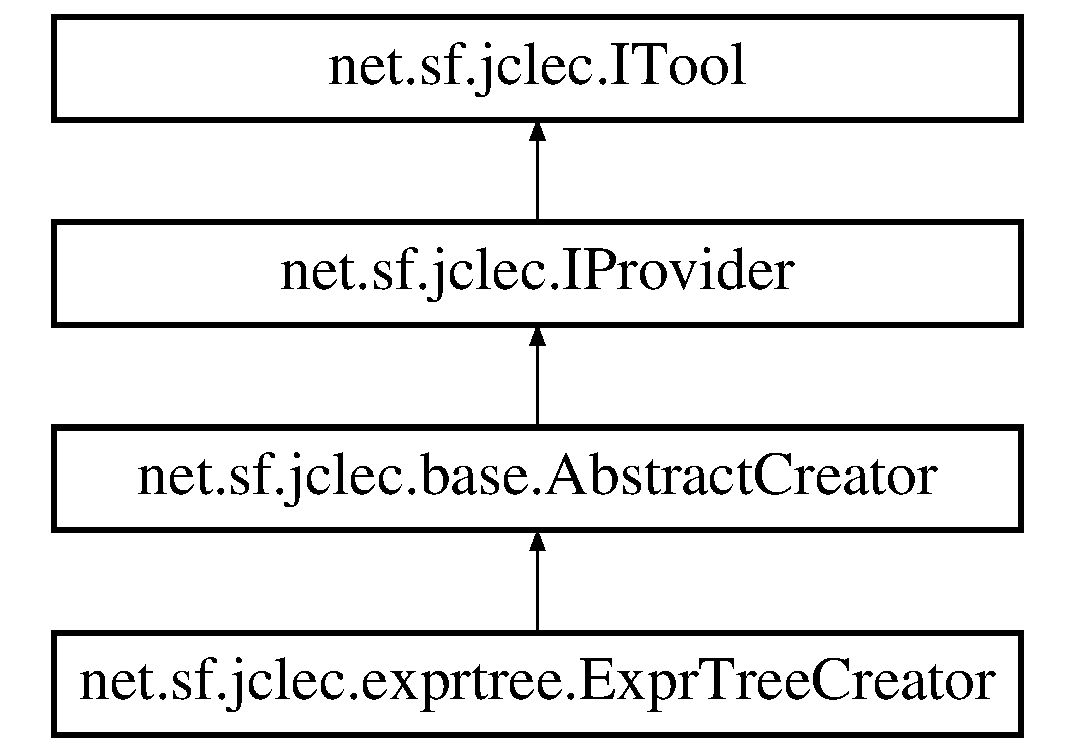
\includegraphics[height=4.000000cm]{classnet_1_1sf_1_1jclec_1_1exprtree_1_1_expr_tree_creator}
\end{center}
\end{figure}
\subsection*{Public Member Functions}
\begin{DoxyCompactItemize}
\item 
\hyperlink{classnet_1_1sf_1_1jclec_1_1exprtree_1_1_expr_tree_creator_a0c3dfd902ef8e98a574c84a410112589}{Expr\-Tree\-Creator} ()
\item 
boolean \hyperlink{classnet_1_1sf_1_1jclec_1_1exprtree_1_1_expr_tree_creator_ae8b64669effe635a411cde20bc3067c1}{equals} (Object other)
\end{DoxyCompactItemize}
\subsection*{Protected Member Functions}
\begin{DoxyCompactItemize}
\item 
void \hyperlink{classnet_1_1sf_1_1jclec_1_1exprtree_1_1_expr_tree_creator_a00264d7b01aa199cc1263302a503e378}{prepare\-Creation} ()
\item 
void \hyperlink{classnet_1_1sf_1_1jclec_1_1exprtree_1_1_expr_tree_creator_afbb105f831c250f0ec1309536359bd63}{create\-Next} ()
\end{DoxyCompactItemize}
\subsection*{Protected Attributes}
\begin{DoxyCompactItemize}
\item 
transient \hyperlink{classnet_1_1sf_1_1jclec_1_1exprtree_1_1_expr_tree_species}{Expr\-Tree\-Species} \hyperlink{classnet_1_1sf_1_1jclec_1_1exprtree_1_1_expr_tree_creator_aa789d23c2a90bcb9a8e964f672f05c1b}{species}
\item 
transient \hyperlink{classnet_1_1sf_1_1jclec_1_1exprtree_1_1_expr_tree_schema}{Expr\-Tree\-Schema} \hyperlink{classnet_1_1sf_1_1jclec_1_1exprtree_1_1_expr_tree_creator_af48de82c56c6d19eae9dd03d871cc7b1}{schema}
\end{DoxyCompactItemize}


\subsection{Detailed Description}
Expression tree individuals creator.

\begin{DoxyAuthor}{Author}
Sebastian Ventura 
\end{DoxyAuthor}


\subsection{Constructor \& Destructor Documentation}
\hypertarget{classnet_1_1sf_1_1jclec_1_1exprtree_1_1_expr_tree_creator_a0c3dfd902ef8e98a574c84a410112589}{\index{net\-::sf\-::jclec\-::exprtree\-::\-Expr\-Tree\-Creator@{net\-::sf\-::jclec\-::exprtree\-::\-Expr\-Tree\-Creator}!Expr\-Tree\-Creator@{Expr\-Tree\-Creator}}
\index{Expr\-Tree\-Creator@{Expr\-Tree\-Creator}!net::sf::jclec::exprtree::ExprTreeCreator@{net\-::sf\-::jclec\-::exprtree\-::\-Expr\-Tree\-Creator}}
\subsubsection[{Expr\-Tree\-Creator}]{\setlength{\rightskip}{0pt plus 5cm}net.\-sf.\-jclec.\-exprtree.\-Expr\-Tree\-Creator.\-Expr\-Tree\-Creator (
\begin{DoxyParamCaption}
{}
\end{DoxyParamCaption}
)}}\label{classnet_1_1sf_1_1jclec_1_1exprtree_1_1_expr_tree_creator_a0c3dfd902ef8e98a574c84a410112589}
Empty (default) constructor. 

\subsection{Member Function Documentation}
\hypertarget{classnet_1_1sf_1_1jclec_1_1exprtree_1_1_expr_tree_creator_afbb105f831c250f0ec1309536359bd63}{\index{net\-::sf\-::jclec\-::exprtree\-::\-Expr\-Tree\-Creator@{net\-::sf\-::jclec\-::exprtree\-::\-Expr\-Tree\-Creator}!create\-Next@{create\-Next}}
\index{create\-Next@{create\-Next}!net::sf::jclec::exprtree::ExprTreeCreator@{net\-::sf\-::jclec\-::exprtree\-::\-Expr\-Tree\-Creator}}
\subsubsection[{create\-Next}]{\setlength{\rightskip}{0pt plus 5cm}void net.\-sf.\-jclec.\-exprtree.\-Expr\-Tree\-Creator.\-create\-Next (
\begin{DoxyParamCaption}
{}
\end{DoxyParamCaption}
)\hspace{0.3cm}{\ttfamily [protected]}, {\ttfamily [virtual]}}}\label{classnet_1_1sf_1_1jclec_1_1exprtree_1_1_expr_tree_creator_afbb105f831c250f0ec1309536359bd63}
Creation method.


\begin{DoxyParams}{Parameters}
{\em ind} & Individual to create\\
\hline
\end{DoxyParams}
\begin{DoxyReturn}{Returns}
New individual
\end{DoxyReturn}
 

Implements \hyperlink{classnet_1_1sf_1_1jclec_1_1base_1_1_abstract_creator_aee6bcace778e7421fc5c07e1a4f6fed9}{net.\-sf.\-jclec.\-base.\-Abstract\-Creator}.

\hypertarget{classnet_1_1sf_1_1jclec_1_1exprtree_1_1_expr_tree_creator_ae8b64669effe635a411cde20bc3067c1}{\index{net\-::sf\-::jclec\-::exprtree\-::\-Expr\-Tree\-Creator@{net\-::sf\-::jclec\-::exprtree\-::\-Expr\-Tree\-Creator}!equals@{equals}}
\index{equals@{equals}!net::sf::jclec::exprtree::ExprTreeCreator@{net\-::sf\-::jclec\-::exprtree\-::\-Expr\-Tree\-Creator}}
\subsubsection[{equals}]{\setlength{\rightskip}{0pt plus 5cm}boolean net.\-sf.\-jclec.\-exprtree.\-Expr\-Tree\-Creator.\-equals (
\begin{DoxyParamCaption}
\item[{Object}]{other}
\end{DoxyParamCaption}
)}}\label{classnet_1_1sf_1_1jclec_1_1exprtree_1_1_expr_tree_creator_ae8b64669effe635a411cde20bc3067c1}
\hypertarget{classnet_1_1sf_1_1jclec_1_1exprtree_1_1_expr_tree_creator_a00264d7b01aa199cc1263302a503e378}{\index{net\-::sf\-::jclec\-::exprtree\-::\-Expr\-Tree\-Creator@{net\-::sf\-::jclec\-::exprtree\-::\-Expr\-Tree\-Creator}!prepare\-Creation@{prepare\-Creation}}
\index{prepare\-Creation@{prepare\-Creation}!net::sf::jclec::exprtree::ExprTreeCreator@{net\-::sf\-::jclec\-::exprtree\-::\-Expr\-Tree\-Creator}}
\subsubsection[{prepare\-Creation}]{\setlength{\rightskip}{0pt plus 5cm}void net.\-sf.\-jclec.\-exprtree.\-Expr\-Tree\-Creator.\-prepare\-Creation (
\begin{DoxyParamCaption}
{}
\end{DoxyParamCaption}
)\hspace{0.3cm}{\ttfamily [protected]}, {\ttfamily [virtual]}}}\label{classnet_1_1sf_1_1jclec_1_1exprtree_1_1_expr_tree_creator_a00264d7b01aa199cc1263302a503e378}
Prepare creation process. 

Implements \hyperlink{classnet_1_1sf_1_1jclec_1_1base_1_1_abstract_creator_a75beaef8489c52782e0c7c956c2beaf7}{net.\-sf.\-jclec.\-base.\-Abstract\-Creator}.



\subsection{Member Data Documentation}
\hypertarget{classnet_1_1sf_1_1jclec_1_1exprtree_1_1_expr_tree_creator_af48de82c56c6d19eae9dd03d871cc7b1}{\index{net\-::sf\-::jclec\-::exprtree\-::\-Expr\-Tree\-Creator@{net\-::sf\-::jclec\-::exprtree\-::\-Expr\-Tree\-Creator}!schema@{schema}}
\index{schema@{schema}!net::sf::jclec::exprtree::ExprTreeCreator@{net\-::sf\-::jclec\-::exprtree\-::\-Expr\-Tree\-Creator}}
\subsubsection[{schema}]{\setlength{\rightskip}{0pt plus 5cm}transient {\bf Expr\-Tree\-Schema} net.\-sf.\-jclec.\-exprtree.\-Expr\-Tree\-Creator.\-schema\hspace{0.3cm}{\ttfamily [protected]}}}\label{classnet_1_1sf_1_1jclec_1_1exprtree_1_1_expr_tree_creator_af48de82c56c6d19eae9dd03d871cc7b1}
Individuals schema \hypertarget{classnet_1_1sf_1_1jclec_1_1exprtree_1_1_expr_tree_creator_aa789d23c2a90bcb9a8e964f672f05c1b}{\index{net\-::sf\-::jclec\-::exprtree\-::\-Expr\-Tree\-Creator@{net\-::sf\-::jclec\-::exprtree\-::\-Expr\-Tree\-Creator}!species@{species}}
\index{species@{species}!net::sf::jclec::exprtree::ExprTreeCreator@{net\-::sf\-::jclec\-::exprtree\-::\-Expr\-Tree\-Creator}}
\subsubsection[{species}]{\setlength{\rightskip}{0pt plus 5cm}transient {\bf Expr\-Tree\-Species} net.\-sf.\-jclec.\-exprtree.\-Expr\-Tree\-Creator.\-species\hspace{0.3cm}{\ttfamily [protected]}}}\label{classnet_1_1sf_1_1jclec_1_1exprtree_1_1_expr_tree_creator_aa789d23c2a90bcb9a8e964f672f05c1b}
Individual species 

The documentation for this class was generated from the following file\-:\begin{DoxyCompactItemize}
\item 
src/main/java/net/sf/jclec/exprtree/Expr\-Tree\-Creator.\-java\end{DoxyCompactItemize}

\hypertarget{classnet_1_1sf_1_1jclec_1_1exprtree_1_1_expr_tree_creator_test}{\section{net.\-sf.\-jclec.\-exprtree.\-Expr\-Tree\-Creator\-Test Class Reference}
\label{classnet_1_1sf_1_1jclec_1_1exprtree_1_1_expr_tree_creator_test}\index{net.\-sf.\-jclec.\-exprtree.\-Expr\-Tree\-Creator\-Test@{net.\-sf.\-jclec.\-exprtree.\-Expr\-Tree\-Creator\-Test}}
}


Inherits I\-Provider\-Test$<$ Expr\-Tree\-Creator $>$.



\subsection{Detailed Description}
\hyperlink{classnet_1_1sf_1_1jclec_1_1exprtree_1_1_expr_tree_creator}{Expr\-Tree\-Creator} tests.

\begin{DoxyAuthor}{Author}
Sebastian Ventura 
\end{DoxyAuthor}


The documentation for this class was generated from the following file\-:\begin{DoxyCompactItemize}
\item 
src/test/java/net/sf/jclec/exprtree/Expr\-Tree\-Creator\-Test.\-java\end{DoxyCompactItemize}

\hypertarget{classnet_1_1sf_1_1jclec_1_1exprtree_1_1fun_1_1_expr_tree_function}{\section{net.\-sf.\-jclec.\-exprtree.\-fun.\-Expr\-Tree\-Function Class Reference}
\label{classnet_1_1sf_1_1jclec_1_1exprtree_1_1fun_1_1_expr_tree_function}\index{net.\-sf.\-jclec.\-exprtree.\-fun.\-Expr\-Tree\-Function@{net.\-sf.\-jclec.\-exprtree.\-fun.\-Expr\-Tree\-Function}}
}
Inheritance diagram for net.\-sf.\-jclec.\-exprtree.\-fun.\-Expr\-Tree\-Function\-:\begin{figure}[H]
\begin{center}
\leavevmode
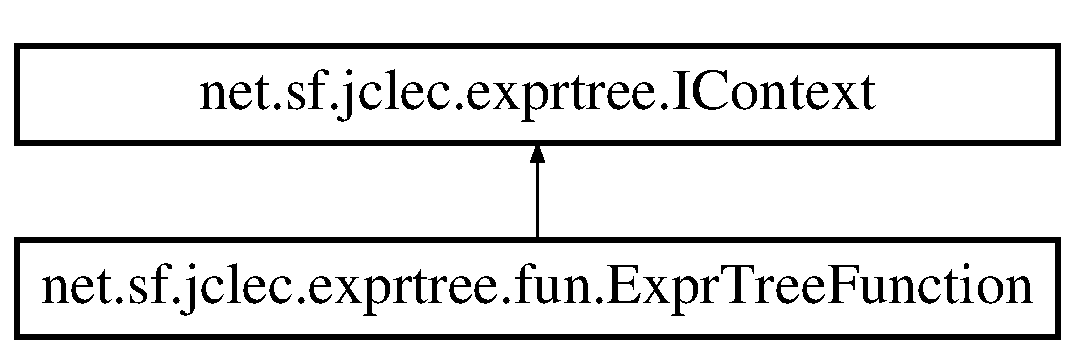
\includegraphics[height=3.000000cm]{classnet_1_1sf_1_1jclec_1_1exprtree_1_1fun_1_1_expr_tree_function}
\end{center}
\end{figure}
\subsection*{Public Member Functions}
\begin{DoxyCompactItemize}
\item 
\hyperlink{classnet_1_1sf_1_1jclec_1_1exprtree_1_1fun_1_1_expr_tree_function_a5466bce31de5c7bfeba0135881074368}{Expr\-Tree\-Function} ()
\item 
\hyperlink{classnet_1_1sf_1_1jclec_1_1exprtree_1_1fun_1_1_expr_tree_function_a15f7749f19ecb2eb46a83f6e286b1194}{Expr\-Tree\-Function} (\hyperlink{classnet_1_1sf_1_1jclec_1_1exprtree_1_1_expr_tree}{Expr\-Tree} \hyperlink{classnet_1_1sf_1_1jclec_1_1exprtree_1_1fun_1_1_expr_tree_function_a148bc528b69b2c629888767cc5e9adbc}{code})
\item 
\hyperlink{classnet_1_1sf_1_1jclec_1_1exprtree_1_1_expr_tree}{Expr\-Tree} \hyperlink{classnet_1_1sf_1_1jclec_1_1exprtree_1_1fun_1_1_expr_tree_function_ab3e0d6e96614c14b5d57a904c1297f50}{get\-Code} ()
\item 
void \hyperlink{classnet_1_1sf_1_1jclec_1_1exprtree_1_1fun_1_1_expr_tree_function_ae5efd1c619720855ca51de3b5d710ca2}{set\-Code} (\hyperlink{classnet_1_1sf_1_1jclec_1_1exprtree_1_1_expr_tree}{Expr\-Tree} \hyperlink{classnet_1_1sf_1_1jclec_1_1exprtree_1_1fun_1_1_expr_tree_function_a148bc528b69b2c629888767cc5e9adbc}{code})
\end{DoxyCompactItemize}
\subsection*{Protected Attributes}
\begin{DoxyCompactItemize}
\item 
\hyperlink{classnet_1_1sf_1_1jclec_1_1exprtree_1_1_expr_tree}{Expr\-Tree} \hyperlink{classnet_1_1sf_1_1jclec_1_1exprtree_1_1fun_1_1_expr_tree_function_a148bc528b69b2c629888767cc5e9adbc}{code}
\item 
Stack$<$ Object $>$ \hyperlink{classnet_1_1sf_1_1jclec_1_1exprtree_1_1fun_1_1_expr_tree_function_aa023e2e693295e66c955ccdff8069274}{stack} = new Stack$<$Object$>$ ()
\item 
Object\mbox{[}$\,$\mbox{]} \hyperlink{classnet_1_1sf_1_1jclec_1_1exprtree_1_1fun_1_1_expr_tree_function_af323c93fc6b862090d0b97f2c774443a}{args}
\end{DoxyCompactItemize}


\subsection{Detailed Description}
Expression tree function.

\begin{DoxyAuthor}{Author}
Sebastian Ventura 
\end{DoxyAuthor}


\subsection{Constructor \& Destructor Documentation}
\hypertarget{classnet_1_1sf_1_1jclec_1_1exprtree_1_1fun_1_1_expr_tree_function_a5466bce31de5c7bfeba0135881074368}{\index{net\-::sf\-::jclec\-::exprtree\-::fun\-::\-Expr\-Tree\-Function@{net\-::sf\-::jclec\-::exprtree\-::fun\-::\-Expr\-Tree\-Function}!Expr\-Tree\-Function@{Expr\-Tree\-Function}}
\index{Expr\-Tree\-Function@{Expr\-Tree\-Function}!net::sf::jclec::exprtree::fun::ExprTreeFunction@{net\-::sf\-::jclec\-::exprtree\-::fun\-::\-Expr\-Tree\-Function}}
\subsubsection[{Expr\-Tree\-Function}]{\setlength{\rightskip}{0pt plus 5cm}net.\-sf.\-jclec.\-exprtree.\-fun.\-Expr\-Tree\-Function.\-Expr\-Tree\-Function (
\begin{DoxyParamCaption}
{}
\end{DoxyParamCaption}
)}}\label{classnet_1_1sf_1_1jclec_1_1exprtree_1_1fun_1_1_expr_tree_function_a5466bce31de5c7bfeba0135881074368}
Empty (default) constructor \hypertarget{classnet_1_1sf_1_1jclec_1_1exprtree_1_1fun_1_1_expr_tree_function_a15f7749f19ecb2eb46a83f6e286b1194}{\index{net\-::sf\-::jclec\-::exprtree\-::fun\-::\-Expr\-Tree\-Function@{net\-::sf\-::jclec\-::exprtree\-::fun\-::\-Expr\-Tree\-Function}!Expr\-Tree\-Function@{Expr\-Tree\-Function}}
\index{Expr\-Tree\-Function@{Expr\-Tree\-Function}!net::sf::jclec::exprtree::fun::ExprTreeFunction@{net\-::sf\-::jclec\-::exprtree\-::fun\-::\-Expr\-Tree\-Function}}
\subsubsection[{Expr\-Tree\-Function}]{\setlength{\rightskip}{0pt plus 5cm}net.\-sf.\-jclec.\-exprtree.\-fun.\-Expr\-Tree\-Function.\-Expr\-Tree\-Function (
\begin{DoxyParamCaption}
\item[{{\bf Expr\-Tree}}]{code}
\end{DoxyParamCaption}
)}}\label{classnet_1_1sf_1_1jclec_1_1exprtree_1_1fun_1_1_expr_tree_function_a15f7749f19ecb2eb46a83f6e286b1194}
Constructor that sets function code 

\subsection{Member Function Documentation}
\hypertarget{classnet_1_1sf_1_1jclec_1_1exprtree_1_1fun_1_1_expr_tree_function_ab3e0d6e96614c14b5d57a904c1297f50}{\index{net\-::sf\-::jclec\-::exprtree\-::fun\-::\-Expr\-Tree\-Function@{net\-::sf\-::jclec\-::exprtree\-::fun\-::\-Expr\-Tree\-Function}!get\-Code@{get\-Code}}
\index{get\-Code@{get\-Code}!net::sf::jclec::exprtree::fun::ExprTreeFunction@{net\-::sf\-::jclec\-::exprtree\-::fun\-::\-Expr\-Tree\-Function}}
\subsubsection[{get\-Code}]{\setlength{\rightskip}{0pt plus 5cm}{\bf Expr\-Tree} net.\-sf.\-jclec.\-exprtree.\-fun.\-Expr\-Tree\-Function.\-get\-Code (
\begin{DoxyParamCaption}
{}
\end{DoxyParamCaption}
)}}\label{classnet_1_1sf_1_1jclec_1_1exprtree_1_1fun_1_1_expr_tree_function_ab3e0d6e96614c14b5d57a904c1297f50}
Access to function code

\begin{DoxyReturn}{Returns}
Current code 
\end{DoxyReturn}
\hypertarget{classnet_1_1sf_1_1jclec_1_1exprtree_1_1fun_1_1_expr_tree_function_ae5efd1c619720855ca51de3b5d710ca2}{\index{net\-::sf\-::jclec\-::exprtree\-::fun\-::\-Expr\-Tree\-Function@{net\-::sf\-::jclec\-::exprtree\-::fun\-::\-Expr\-Tree\-Function}!set\-Code@{set\-Code}}
\index{set\-Code@{set\-Code}!net::sf::jclec::exprtree::fun::ExprTreeFunction@{net\-::sf\-::jclec\-::exprtree\-::fun\-::\-Expr\-Tree\-Function}}
\subsubsection[{set\-Code}]{\setlength{\rightskip}{0pt plus 5cm}void net.\-sf.\-jclec.\-exprtree.\-fun.\-Expr\-Tree\-Function.\-set\-Code (
\begin{DoxyParamCaption}
\item[{{\bf Expr\-Tree}}]{code}
\end{DoxyParamCaption}
)}}\label{classnet_1_1sf_1_1jclec_1_1exprtree_1_1fun_1_1_expr_tree_function_ae5efd1c619720855ca51de3b5d710ca2}
Sets function code


\begin{DoxyParams}{Parameters}
{\em code} & Function code \\
\hline
\end{DoxyParams}


\subsection{Member Data Documentation}
\hypertarget{classnet_1_1sf_1_1jclec_1_1exprtree_1_1fun_1_1_expr_tree_function_af323c93fc6b862090d0b97f2c774443a}{\index{net\-::sf\-::jclec\-::exprtree\-::fun\-::\-Expr\-Tree\-Function@{net\-::sf\-::jclec\-::exprtree\-::fun\-::\-Expr\-Tree\-Function}!args@{args}}
\index{args@{args}!net::sf::jclec::exprtree::fun::ExprTreeFunction@{net\-::sf\-::jclec\-::exprtree\-::fun\-::\-Expr\-Tree\-Function}}
\subsubsection[{args}]{\setlength{\rightskip}{0pt plus 5cm}Object \mbox{[}$\,$\mbox{]} net.\-sf.\-jclec.\-exprtree.\-fun.\-Expr\-Tree\-Function.\-args\hspace{0.3cm}{\ttfamily [protected]}}}\label{classnet_1_1sf_1_1jclec_1_1exprtree_1_1fun_1_1_expr_tree_function_af323c93fc6b862090d0b97f2c774443a}
Current arguments \hypertarget{classnet_1_1sf_1_1jclec_1_1exprtree_1_1fun_1_1_expr_tree_function_a148bc528b69b2c629888767cc5e9adbc}{\index{net\-::sf\-::jclec\-::exprtree\-::fun\-::\-Expr\-Tree\-Function@{net\-::sf\-::jclec\-::exprtree\-::fun\-::\-Expr\-Tree\-Function}!code@{code}}
\index{code@{code}!net::sf::jclec::exprtree::fun::ExprTreeFunction@{net\-::sf\-::jclec\-::exprtree\-::fun\-::\-Expr\-Tree\-Function}}
\subsubsection[{code}]{\setlength{\rightskip}{0pt plus 5cm}{\bf Expr\-Tree} net.\-sf.\-jclec.\-exprtree.\-fun.\-Expr\-Tree\-Function.\-code\hspace{0.3cm}{\ttfamily [protected]}}}\label{classnet_1_1sf_1_1jclec_1_1exprtree_1_1fun_1_1_expr_tree_function_a148bc528b69b2c629888767cc5e9adbc}
Function code \hypertarget{classnet_1_1sf_1_1jclec_1_1exprtree_1_1fun_1_1_expr_tree_function_aa023e2e693295e66c955ccdff8069274}{\index{net\-::sf\-::jclec\-::exprtree\-::fun\-::\-Expr\-Tree\-Function@{net\-::sf\-::jclec\-::exprtree\-::fun\-::\-Expr\-Tree\-Function}!stack@{stack}}
\index{stack@{stack}!net::sf::jclec::exprtree::fun::ExprTreeFunction@{net\-::sf\-::jclec\-::exprtree\-::fun\-::\-Expr\-Tree\-Function}}
\subsubsection[{stack}]{\setlength{\rightskip}{0pt plus 5cm}Stack$<$Object$>$ net.\-sf.\-jclec.\-exprtree.\-fun.\-Expr\-Tree\-Function.\-stack = new Stack$<$Object$>$ ()\hspace{0.3cm}{\ttfamily [protected]}}}\label{classnet_1_1sf_1_1jclec_1_1exprtree_1_1fun_1_1_expr_tree_function_aa023e2e693295e66c955ccdff8069274}
Execution stack 

The documentation for this class was generated from the following file\-:\begin{DoxyCompactItemize}
\item 
src/main/java/net/sf/jclec/exprtree/fun/Expr\-Tree\-Function.\-java\end{DoxyCompactItemize}

\hypertarget{classnet_1_1sf_1_1jclec_1_1exprtree_1_1_expr_tree_individual}{\section{net.\-sf.\-jclec.\-exprtree.\-Expr\-Tree\-Individual Class Reference}
\label{classnet_1_1sf_1_1jclec_1_1exprtree_1_1_expr_tree_individual}\index{net.\-sf.\-jclec.\-exprtree.\-Expr\-Tree\-Individual@{net.\-sf.\-jclec.\-exprtree.\-Expr\-Tree\-Individual}}
}


Inherits Abstract\-Individual$<$ Expr\-Tree $>$.

\subsection*{Public Member Functions}
\begin{DoxyCompactItemize}
\item 
\hyperlink{classnet_1_1sf_1_1jclec_1_1exprtree_1_1_expr_tree_individual_a90f6adb50d1bb1006f2f7b570a63a30b}{Expr\-Tree\-Individual} ()
\item 
\hyperlink{classnet_1_1sf_1_1jclec_1_1exprtree_1_1_expr_tree_individual_a677fd6fed93235286269875d8e0aaace}{Expr\-Tree\-Individual} (\hyperlink{classnet_1_1sf_1_1jclec_1_1exprtree_1_1_expr_tree}{Expr\-Tree} genotype)
\item 
\hyperlink{classnet_1_1sf_1_1jclec_1_1exprtree_1_1_expr_tree_individual_acaa907c4991ac92450ab58de3fb20fa8}{Expr\-Tree\-Individual} (\hyperlink{classnet_1_1sf_1_1jclec_1_1exprtree_1_1_expr_tree}{Expr\-Tree} genotype, \hyperlink{interfacenet_1_1sf_1_1jclec_1_1_i_fitness}{I\-Fitness} fitness)
\item 
double \hyperlink{classnet_1_1sf_1_1jclec_1_1exprtree_1_1_expr_tree_individual_ae0ad5d9b4da029b8d71f81ce83189d63}{distance} (\hyperlink{interfacenet_1_1sf_1_1jclec_1_1_i_individual}{I\-Individual} other)
\item 
\hyperlink{interfacenet_1_1sf_1_1jclec_1_1_i_individual}{I\-Individual} \hyperlink{classnet_1_1sf_1_1jclec_1_1exprtree_1_1_expr_tree_individual_aa58c74282bb238ce2f44cc6db1e6890a}{copy} ()
\item 
boolean \hyperlink{classnet_1_1sf_1_1jclec_1_1exprtree_1_1_expr_tree_individual_ac183d4db7b77f8000827755588551efc}{equals} (Object other)
\item 
String \hyperlink{classnet_1_1sf_1_1jclec_1_1exprtree_1_1_expr_tree_individual_a5cb900ef9079188e4f4e69eba1397701}{to\-String} ()
\end{DoxyCompactItemize}


\subsection{Detailed Description}
Individual that contains one expression tree as genotype.

\begin{DoxyAuthor}{Author}
Sebastian Ventura 
\end{DoxyAuthor}


\subsection{Constructor \& Destructor Documentation}
\hypertarget{classnet_1_1sf_1_1jclec_1_1exprtree_1_1_expr_tree_individual_a90f6adb50d1bb1006f2f7b570a63a30b}{\index{net\-::sf\-::jclec\-::exprtree\-::\-Expr\-Tree\-Individual@{net\-::sf\-::jclec\-::exprtree\-::\-Expr\-Tree\-Individual}!Expr\-Tree\-Individual@{Expr\-Tree\-Individual}}
\index{Expr\-Tree\-Individual@{Expr\-Tree\-Individual}!net::sf::jclec::exprtree::ExprTreeIndividual@{net\-::sf\-::jclec\-::exprtree\-::\-Expr\-Tree\-Individual}}
\subsubsection[{Expr\-Tree\-Individual}]{\setlength{\rightskip}{0pt plus 5cm}net.\-sf.\-jclec.\-exprtree.\-Expr\-Tree\-Individual.\-Expr\-Tree\-Individual (
\begin{DoxyParamCaption}
{}
\end{DoxyParamCaption}
)}}\label{classnet_1_1sf_1_1jclec_1_1exprtree_1_1_expr_tree_individual_a90f6adb50d1bb1006f2f7b570a63a30b}
Empty constructor. \hypertarget{classnet_1_1sf_1_1jclec_1_1exprtree_1_1_expr_tree_individual_a677fd6fed93235286269875d8e0aaace}{\index{net\-::sf\-::jclec\-::exprtree\-::\-Expr\-Tree\-Individual@{net\-::sf\-::jclec\-::exprtree\-::\-Expr\-Tree\-Individual}!Expr\-Tree\-Individual@{Expr\-Tree\-Individual}}
\index{Expr\-Tree\-Individual@{Expr\-Tree\-Individual}!net::sf::jclec::exprtree::ExprTreeIndividual@{net\-::sf\-::jclec\-::exprtree\-::\-Expr\-Tree\-Individual}}
\subsubsection[{Expr\-Tree\-Individual}]{\setlength{\rightskip}{0pt plus 5cm}net.\-sf.\-jclec.\-exprtree.\-Expr\-Tree\-Individual.\-Expr\-Tree\-Individual (
\begin{DoxyParamCaption}
\item[{{\bf Expr\-Tree}}]{genotype}
\end{DoxyParamCaption}
)}}\label{classnet_1_1sf_1_1jclec_1_1exprtree_1_1_expr_tree_individual_a677fd6fed93235286269875d8e0aaace}
Constructor that sets individual genotype.


\begin{DoxyParams}{Parameters}
{\em genotype} & Individual genotype \\
\hline
\end{DoxyParams}
\hypertarget{classnet_1_1sf_1_1jclec_1_1exprtree_1_1_expr_tree_individual_acaa907c4991ac92450ab58de3fb20fa8}{\index{net\-::sf\-::jclec\-::exprtree\-::\-Expr\-Tree\-Individual@{net\-::sf\-::jclec\-::exprtree\-::\-Expr\-Tree\-Individual}!Expr\-Tree\-Individual@{Expr\-Tree\-Individual}}
\index{Expr\-Tree\-Individual@{Expr\-Tree\-Individual}!net::sf::jclec::exprtree::ExprTreeIndividual@{net\-::sf\-::jclec\-::exprtree\-::\-Expr\-Tree\-Individual}}
\subsubsection[{Expr\-Tree\-Individual}]{\setlength{\rightskip}{0pt plus 5cm}net.\-sf.\-jclec.\-exprtree.\-Expr\-Tree\-Individual.\-Expr\-Tree\-Individual (
\begin{DoxyParamCaption}
\item[{{\bf Expr\-Tree}}]{genotype, }
\item[{{\bf I\-Fitness}}]{fitness}
\end{DoxyParamCaption}
)}}\label{classnet_1_1sf_1_1jclec_1_1exprtree_1_1_expr_tree_individual_acaa907c4991ac92450ab58de3fb20fa8}
Constructor that sets individual genotype and fitness.


\begin{DoxyParams}{Parameters}
{\em genotype} & Individual genotype \\
\hline
{\em fitness} & Individual fitness \\
\hline
\end{DoxyParams}


\subsection{Member Function Documentation}
\hypertarget{classnet_1_1sf_1_1jclec_1_1exprtree_1_1_expr_tree_individual_aa58c74282bb238ce2f44cc6db1e6890a}{\index{net\-::sf\-::jclec\-::exprtree\-::\-Expr\-Tree\-Individual@{net\-::sf\-::jclec\-::exprtree\-::\-Expr\-Tree\-Individual}!copy@{copy}}
\index{copy@{copy}!net::sf::jclec::exprtree::ExprTreeIndividual@{net\-::sf\-::jclec\-::exprtree\-::\-Expr\-Tree\-Individual}}
\subsubsection[{copy}]{\setlength{\rightskip}{0pt plus 5cm}{\bf I\-Individual} net.\-sf.\-jclec.\-exprtree.\-Expr\-Tree\-Individual.\-copy (
\begin{DoxyParamCaption}
{}
\end{DoxyParamCaption}
)}}\label{classnet_1_1sf_1_1jclec_1_1exprtree_1_1_expr_tree_individual_aa58c74282bb238ce2f44cc6db1e6890a}
\hypertarget{classnet_1_1sf_1_1jclec_1_1exprtree_1_1_expr_tree_individual_ae0ad5d9b4da029b8d71f81ce83189d63}{\index{net\-::sf\-::jclec\-::exprtree\-::\-Expr\-Tree\-Individual@{net\-::sf\-::jclec\-::exprtree\-::\-Expr\-Tree\-Individual}!distance@{distance}}
\index{distance@{distance}!net::sf::jclec::exprtree::ExprTreeIndividual@{net\-::sf\-::jclec\-::exprtree\-::\-Expr\-Tree\-Individual}}
\subsubsection[{distance}]{\setlength{\rightskip}{0pt plus 5cm}double net.\-sf.\-jclec.\-exprtree.\-Expr\-Tree\-Individual.\-distance (
\begin{DoxyParamCaption}
\item[{{\bf I\-Individual}}]{other}
\end{DoxyParamCaption}
)}}\label{classnet_1_1sf_1_1jclec_1_1exprtree_1_1_expr_tree_individual_ae0ad5d9b4da029b8d71f81ce83189d63}
\hypertarget{classnet_1_1sf_1_1jclec_1_1exprtree_1_1_expr_tree_individual_ac183d4db7b77f8000827755588551efc}{\index{net\-::sf\-::jclec\-::exprtree\-::\-Expr\-Tree\-Individual@{net\-::sf\-::jclec\-::exprtree\-::\-Expr\-Tree\-Individual}!equals@{equals}}
\index{equals@{equals}!net::sf::jclec::exprtree::ExprTreeIndividual@{net\-::sf\-::jclec\-::exprtree\-::\-Expr\-Tree\-Individual}}
\subsubsection[{equals}]{\setlength{\rightskip}{0pt plus 5cm}boolean net.\-sf.\-jclec.\-exprtree.\-Expr\-Tree\-Individual.\-equals (
\begin{DoxyParamCaption}
\item[{Object}]{other}
\end{DoxyParamCaption}
)}}\label{classnet_1_1sf_1_1jclec_1_1exprtree_1_1_expr_tree_individual_ac183d4db7b77f8000827755588551efc}
\hypertarget{classnet_1_1sf_1_1jclec_1_1exprtree_1_1_expr_tree_individual_a5cb900ef9079188e4f4e69eba1397701}{\index{net\-::sf\-::jclec\-::exprtree\-::\-Expr\-Tree\-Individual@{net\-::sf\-::jclec\-::exprtree\-::\-Expr\-Tree\-Individual}!to\-String@{to\-String}}
\index{to\-String@{to\-String}!net::sf::jclec::exprtree::ExprTreeIndividual@{net\-::sf\-::jclec\-::exprtree\-::\-Expr\-Tree\-Individual}}
\subsubsection[{to\-String}]{\setlength{\rightskip}{0pt plus 5cm}String net.\-sf.\-jclec.\-exprtree.\-Expr\-Tree\-Individual.\-to\-String (
\begin{DoxyParamCaption}
{}
\end{DoxyParamCaption}
)}}\label{classnet_1_1sf_1_1jclec_1_1exprtree_1_1_expr_tree_individual_a5cb900ef9079188e4f4e69eba1397701}


The documentation for this class was generated from the following file\-:\begin{DoxyCompactItemize}
\item 
src/main/java/net/sf/jclec/exprtree/Expr\-Tree\-Individual.\-java\end{DoxyCompactItemize}

\hypertarget{classnet_1_1sf_1_1jclec_1_1exprtree_1_1_expr_tree_individual_species}{\section{net.\-sf.\-jclec.\-exprtree.\-Expr\-Tree\-Individual\-Species Class Reference}
\label{classnet_1_1sf_1_1jclec_1_1exprtree_1_1_expr_tree_individual_species}\index{net.\-sf.\-jclec.\-exprtree.\-Expr\-Tree\-Individual\-Species@{net.\-sf.\-jclec.\-exprtree.\-Expr\-Tree\-Individual\-Species}}
}
Inheritance diagram for net.\-sf.\-jclec.\-exprtree.\-Expr\-Tree\-Individual\-Species\-:\begin{figure}[H]
\begin{center}
\leavevmode
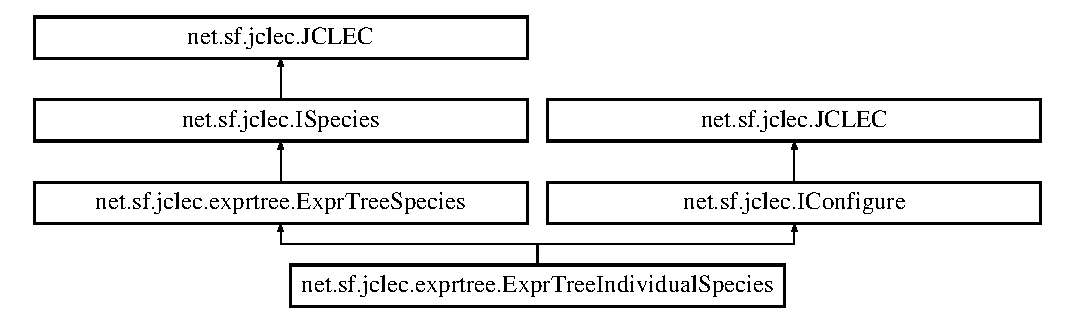
\includegraphics[height=2.916667cm]{classnet_1_1sf_1_1jclec_1_1exprtree_1_1_expr_tree_individual_species}
\end{center}
\end{figure}
\subsection*{Public Member Functions}
\begin{DoxyCompactItemize}
\item 
\hyperlink{classnet_1_1sf_1_1jclec_1_1exprtree_1_1_expr_tree_individual_species_a84656e077221abff562f864629d0144a}{Expr\-Tree\-Individual\-Species} ()
\item 
void \hyperlink{classnet_1_1sf_1_1jclec_1_1exprtree_1_1_expr_tree_individual_species_a9e294e2d9ff9b46e8a6e296714a9099a}{set\-Root\-Type} (Class$<$?$>$ root\-Type)
\item 
void \hyperlink{classnet_1_1sf_1_1jclec_1_1exprtree_1_1_expr_tree_individual_species_a8215ed33917e3083423cb5b6705a0ccd}{set\-Terminals} (\hyperlink{interfacenet_1_1sf_1_1jclec_1_1exprtree_1_1_i_primitive}{I\-Primitive}\mbox{[}$\,$\mbox{]} terminals)
\item 
void \hyperlink{classnet_1_1sf_1_1jclec_1_1exprtree_1_1_expr_tree_individual_species_ae6e240a2c491c3fcd904ce51ae3711c3}{set\-Functions} (\hyperlink{interfacenet_1_1sf_1_1jclec_1_1exprtree_1_1_i_primitive}{I\-Primitive}\mbox{[}$\,$\mbox{]} functions)
\item 
\hyperlink{classnet_1_1sf_1_1jclec_1_1exprtree_1_1_expr_tree_individual}{Expr\-Tree\-Individual} \hyperlink{classnet_1_1sf_1_1jclec_1_1exprtree_1_1_expr_tree_individual_species_a6936c4b65390bca20a51bf0bccc43680}{create\-Individual} ()
\item 
\hyperlink{classnet_1_1sf_1_1jclec_1_1exprtree_1_1_expr_tree_individual}{Expr\-Tree\-Individual} \hyperlink{classnet_1_1sf_1_1jclec_1_1exprtree_1_1_expr_tree_individual_species_a1fb358ef3ae35458367cc916fa194884}{create\-Individual} (\hyperlink{classnet_1_1sf_1_1jclec_1_1exprtree_1_1_expr_tree}{Expr\-Tree} genotype)
\item 
void \hyperlink{classnet_1_1sf_1_1jclec_1_1exprtree_1_1_expr_tree_individual_species_a7f28787d5d80d52e655d2ebf889f0ae0}{configure} (Configuration settings)
\item 
boolean \hyperlink{classnet_1_1sf_1_1jclec_1_1exprtree_1_1_expr_tree_individual_species_a2eea8118c76cc7f4f3249fde0b8afb64}{equals} (Object other)
\end{DoxyCompactItemize}
\subsection*{Additional Inherited Members}


\subsection{Detailed Description}
Expre\-Tree\-Individual species.

\begin{DoxyAuthor}{Author}
Sebastian Ventura 
\end{DoxyAuthor}


\subsection{Constructor \& Destructor Documentation}
\hypertarget{classnet_1_1sf_1_1jclec_1_1exprtree_1_1_expr_tree_individual_species_a84656e077221abff562f864629d0144a}{\index{net\-::sf\-::jclec\-::exprtree\-::\-Expr\-Tree\-Individual\-Species@{net\-::sf\-::jclec\-::exprtree\-::\-Expr\-Tree\-Individual\-Species}!Expr\-Tree\-Individual\-Species@{Expr\-Tree\-Individual\-Species}}
\index{Expr\-Tree\-Individual\-Species@{Expr\-Tree\-Individual\-Species}!net::sf::jclec::exprtree::ExprTreeIndividualSpecies@{net\-::sf\-::jclec\-::exprtree\-::\-Expr\-Tree\-Individual\-Species}}
\subsubsection[{Expr\-Tree\-Individual\-Species}]{\setlength{\rightskip}{0pt plus 5cm}net.\-sf.\-jclec.\-exprtree.\-Expr\-Tree\-Individual\-Species.\-Expr\-Tree\-Individual\-Species (
\begin{DoxyParamCaption}
{}
\end{DoxyParamCaption}
)}}\label{classnet_1_1sf_1_1jclec_1_1exprtree_1_1_expr_tree_individual_species_a84656e077221abff562f864629d0144a}
Empty constructor 

\subsection{Member Function Documentation}
\hypertarget{classnet_1_1sf_1_1jclec_1_1exprtree_1_1_expr_tree_individual_species_a7f28787d5d80d52e655d2ebf889f0ae0}{\index{net\-::sf\-::jclec\-::exprtree\-::\-Expr\-Tree\-Individual\-Species@{net\-::sf\-::jclec\-::exprtree\-::\-Expr\-Tree\-Individual\-Species}!configure@{configure}}
\index{configure@{configure}!net::sf::jclec::exprtree::ExprTreeIndividualSpecies@{net\-::sf\-::jclec\-::exprtree\-::\-Expr\-Tree\-Individual\-Species}}
\subsubsection[{configure}]{\setlength{\rightskip}{0pt plus 5cm}void net.\-sf.\-jclec.\-exprtree.\-Expr\-Tree\-Individual\-Species.\-configure (
\begin{DoxyParamCaption}
\item[{Configuration}]{settings}
\end{DoxyParamCaption}
)}}\label{classnet_1_1sf_1_1jclec_1_1exprtree_1_1_expr_tree_individual_species_a7f28787d5d80d52e655d2ebf889f0ae0}
Configuration method.

Configuration parameters for Pref\-Expr\-Individual\-Species are\-:


\begin{DoxyItemize}
\item 
\end{DoxyItemize}

Implements \hyperlink{interfacenet_1_1sf_1_1jclec_1_1_i_configure_add31a65a04d148c690a956fbbad6987c}{net.\-sf.\-jclec.\-I\-Configure}.

\hypertarget{classnet_1_1sf_1_1jclec_1_1exprtree_1_1_expr_tree_individual_species_a6936c4b65390bca20a51bf0bccc43680}{\index{net\-::sf\-::jclec\-::exprtree\-::\-Expr\-Tree\-Individual\-Species@{net\-::sf\-::jclec\-::exprtree\-::\-Expr\-Tree\-Individual\-Species}!create\-Individual@{create\-Individual}}
\index{create\-Individual@{create\-Individual}!net::sf::jclec::exprtree::ExprTreeIndividualSpecies@{net\-::sf\-::jclec\-::exprtree\-::\-Expr\-Tree\-Individual\-Species}}
\subsubsection[{create\-Individual}]{\setlength{\rightskip}{0pt plus 5cm}{\bf Expr\-Tree\-Individual} net.\-sf.\-jclec.\-exprtree.\-Expr\-Tree\-Individual\-Species.\-create\-Individual (
\begin{DoxyParamCaption}
{}
\end{DoxyParamCaption}
)}}\label{classnet_1_1sf_1_1jclec_1_1exprtree_1_1_expr_tree_individual_species_a6936c4b65390bca20a51bf0bccc43680}
Creates an \hyperlink{classnet_1_1sf_1_1jclec_1_1exprtree_1_1_expr_tree_individual}{Expr\-Tree\-Individual}

\begin{DoxyReturn}{Returns}
new \hyperlink{classnet_1_1sf_1_1jclec_1_1exprtree_1_1_expr_tree_individual}{Expr\-Tree\-Individual} individual 
\end{DoxyReturn}
\hypertarget{classnet_1_1sf_1_1jclec_1_1exprtree_1_1_expr_tree_individual_species_a1fb358ef3ae35458367cc916fa194884}{\index{net\-::sf\-::jclec\-::exprtree\-::\-Expr\-Tree\-Individual\-Species@{net\-::sf\-::jclec\-::exprtree\-::\-Expr\-Tree\-Individual\-Species}!create\-Individual@{create\-Individual}}
\index{create\-Individual@{create\-Individual}!net::sf::jclec::exprtree::ExprTreeIndividualSpecies@{net\-::sf\-::jclec\-::exprtree\-::\-Expr\-Tree\-Individual\-Species}}
\subsubsection[{create\-Individual}]{\setlength{\rightskip}{0pt plus 5cm}{\bf Expr\-Tree\-Individual} net.\-sf.\-jclec.\-exprtree.\-Expr\-Tree\-Individual\-Species.\-create\-Individual (
\begin{DoxyParamCaption}
\item[{{\bf Expr\-Tree}}]{genotype}
\end{DoxyParamCaption}
)\hspace{0.3cm}{\ttfamily [virtual]}}}\label{classnet_1_1sf_1_1jclec_1_1exprtree_1_1_expr_tree_individual_species_a1fb358ef3ae35458367cc916fa194884}
Factory method. Set individual genotype.


\begin{DoxyParams}{Parameters}
{\em genotype} & Individual genotype\\
\hline
\end{DoxyParams}
\begin{DoxyReturn}{Returns}
A new instance of individual class, with its genotype set
\end{DoxyReturn}
 

Implements \hyperlink{classnet_1_1sf_1_1jclec_1_1exprtree_1_1_expr_tree_species_afd641a58862d811f75a112b2dbdd9e0b}{net.\-sf.\-jclec.\-exprtree.\-Expr\-Tree\-Species}.

\hypertarget{classnet_1_1sf_1_1jclec_1_1exprtree_1_1_expr_tree_individual_species_a2eea8118c76cc7f4f3249fde0b8afb64}{\index{net\-::sf\-::jclec\-::exprtree\-::\-Expr\-Tree\-Individual\-Species@{net\-::sf\-::jclec\-::exprtree\-::\-Expr\-Tree\-Individual\-Species}!equals@{equals}}
\index{equals@{equals}!net::sf::jclec::exprtree::ExprTreeIndividualSpecies@{net\-::sf\-::jclec\-::exprtree\-::\-Expr\-Tree\-Individual\-Species}}
\subsubsection[{equals}]{\setlength{\rightskip}{0pt plus 5cm}boolean net.\-sf.\-jclec.\-exprtree.\-Expr\-Tree\-Individual\-Species.\-equals (
\begin{DoxyParamCaption}
\item[{Object}]{other}
\end{DoxyParamCaption}
)}}\label{classnet_1_1sf_1_1jclec_1_1exprtree_1_1_expr_tree_individual_species_a2eea8118c76cc7f4f3249fde0b8afb64}
\hypertarget{classnet_1_1sf_1_1jclec_1_1exprtree_1_1_expr_tree_individual_species_ae6e240a2c491c3fcd904ce51ae3711c3}{\index{net\-::sf\-::jclec\-::exprtree\-::\-Expr\-Tree\-Individual\-Species@{net\-::sf\-::jclec\-::exprtree\-::\-Expr\-Tree\-Individual\-Species}!set\-Functions@{set\-Functions}}
\index{set\-Functions@{set\-Functions}!net::sf::jclec::exprtree::ExprTreeIndividualSpecies@{net\-::sf\-::jclec\-::exprtree\-::\-Expr\-Tree\-Individual\-Species}}
\subsubsection[{set\-Functions}]{\setlength{\rightskip}{0pt plus 5cm}void net.\-sf.\-jclec.\-exprtree.\-Expr\-Tree\-Individual\-Species.\-set\-Functions (
\begin{DoxyParamCaption}
\item[{{\bf I\-Primitive}\mbox{[}$\,$\mbox{]}}]{functions}
\end{DoxyParamCaption}
)}}\label{classnet_1_1sf_1_1jclec_1_1exprtree_1_1_expr_tree_individual_species_ae6e240a2c491c3fcd904ce51ae3711c3}
Set the functions set for an expression tree.


\begin{DoxyParams}{Parameters}
{\em functions} & Functions set for this tree \\
\hline
\end{DoxyParams}
\hypertarget{classnet_1_1sf_1_1jclec_1_1exprtree_1_1_expr_tree_individual_species_a9e294e2d9ff9b46e8a6e296714a9099a}{\index{net\-::sf\-::jclec\-::exprtree\-::\-Expr\-Tree\-Individual\-Species@{net\-::sf\-::jclec\-::exprtree\-::\-Expr\-Tree\-Individual\-Species}!set\-Root\-Type@{set\-Root\-Type}}
\index{set\-Root\-Type@{set\-Root\-Type}!net::sf::jclec::exprtree::ExprTreeIndividualSpecies@{net\-::sf\-::jclec\-::exprtree\-::\-Expr\-Tree\-Individual\-Species}}
\subsubsection[{set\-Root\-Type}]{\setlength{\rightskip}{0pt plus 5cm}void net.\-sf.\-jclec.\-exprtree.\-Expr\-Tree\-Individual\-Species.\-set\-Root\-Type (
\begin{DoxyParamCaption}
\item[{Class$<$?$>$}]{root\-Type}
\end{DoxyParamCaption}
)}}\label{classnet_1_1sf_1_1jclec_1_1exprtree_1_1_expr_tree_individual_species_a9e294e2d9ff9b46e8a6e296714a9099a}
Set the root type for an expression tree.


\begin{DoxyParams}{Parameters}
{\em root\-Type} & Root type for this tree \\
\hline
\end{DoxyParams}
\hypertarget{classnet_1_1sf_1_1jclec_1_1exprtree_1_1_expr_tree_individual_species_a8215ed33917e3083423cb5b6705a0ccd}{\index{net\-::sf\-::jclec\-::exprtree\-::\-Expr\-Tree\-Individual\-Species@{net\-::sf\-::jclec\-::exprtree\-::\-Expr\-Tree\-Individual\-Species}!set\-Terminals@{set\-Terminals}}
\index{set\-Terminals@{set\-Terminals}!net::sf::jclec::exprtree::ExprTreeIndividualSpecies@{net\-::sf\-::jclec\-::exprtree\-::\-Expr\-Tree\-Individual\-Species}}
\subsubsection[{set\-Terminals}]{\setlength{\rightskip}{0pt plus 5cm}void net.\-sf.\-jclec.\-exprtree.\-Expr\-Tree\-Individual\-Species.\-set\-Terminals (
\begin{DoxyParamCaption}
\item[{{\bf I\-Primitive}\mbox{[}$\,$\mbox{]}}]{terminals}
\end{DoxyParamCaption}
)}}\label{classnet_1_1sf_1_1jclec_1_1exprtree_1_1_expr_tree_individual_species_a8215ed33917e3083423cb5b6705a0ccd}
Set the terminals set for an expression tree.


\begin{DoxyParams}{Parameters}
{\em terminals} & Terminals set for this tree \\
\hline
\end{DoxyParams}


The documentation for this class was generated from the following file\-:\begin{DoxyCompactItemize}
\item 
src/main/java/net/sf/jclec/exprtree/Expr\-Tree\-Individual\-Species.\-java\end{DoxyCompactItemize}

\hypertarget{classnet_1_1sf_1_1jclec_1_1exprtree_1_1_expr_tree_mutator}{\section{net.\-sf.\-jclec.\-exprtree.\-Expr\-Tree\-Mutator Class Reference}
\label{classnet_1_1sf_1_1jclec_1_1exprtree_1_1_expr_tree_mutator}\index{net.\-sf.\-jclec.\-exprtree.\-Expr\-Tree\-Mutator@{net.\-sf.\-jclec.\-exprtree.\-Expr\-Tree\-Mutator}}
}
Inheritance diagram for net.\-sf.\-jclec.\-exprtree.\-Expr\-Tree\-Mutator\-:\begin{figure}[H]
\begin{center}
\leavevmode
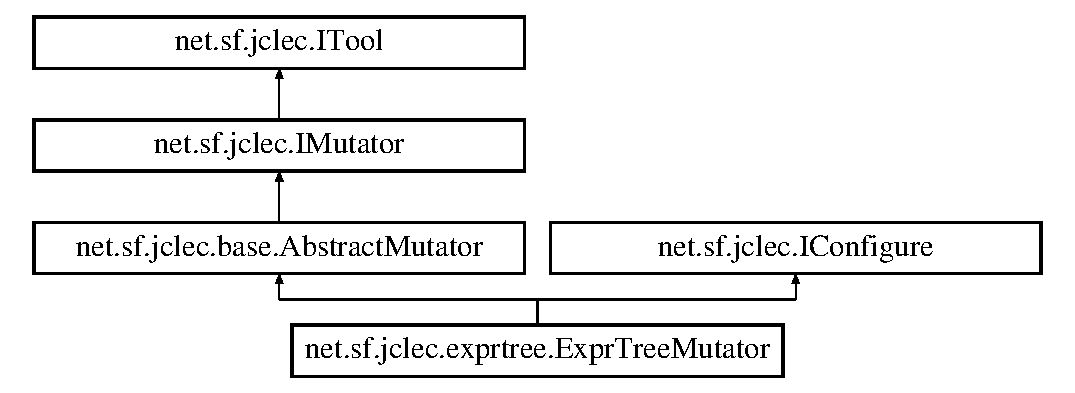
\includegraphics[height=4.000000cm]{classnet_1_1sf_1_1jclec_1_1exprtree_1_1_expr_tree_mutator}
\end{center}
\end{figure}
\subsection*{Public Member Functions}
\begin{DoxyCompactItemize}
\item 
void \hyperlink{classnet_1_1sf_1_1jclec_1_1exprtree_1_1_expr_tree_mutator_ae0c1d1db6bce702193c621c3b9366688}{configure} (Configuration settings)
\end{DoxyCompactItemize}
\subsection*{Protected Member Functions}
\begin{DoxyCompactItemize}
\item 
void \hyperlink{classnet_1_1sf_1_1jclec_1_1exprtree_1_1_expr_tree_mutator_a2bafce5d54003041106517857e0ce65b}{prepare\-Mutation} ()
\item 
void \hyperlink{classnet_1_1sf_1_1jclec_1_1exprtree_1_1_expr_tree_mutator_a51f55d91527bfbd7656f6cd11c4ebb3d}{mutate\-Next} ()
\end{DoxyCompactItemize}
\subsection*{Protected Attributes}
\begin{DoxyCompactItemize}
\item 
\hyperlink{interfacenet_1_1sf_1_1jclec_1_1exprtree_1_1_i_mutate_expr_tree}{I\-Mutate\-Expr\-Tree} \hyperlink{classnet_1_1sf_1_1jclec_1_1exprtree_1_1_expr_tree_mutator_afe98b10b638ef653fe71286d82d2fd93}{base\-Op}
\item 
transient \hyperlink{classnet_1_1sf_1_1jclec_1_1exprtree_1_1_expr_tree_species}{Expr\-Tree\-Species} \hyperlink{classnet_1_1sf_1_1jclec_1_1exprtree_1_1_expr_tree_mutator_a45ee9a1b04a9a6d880993e17ee60bf7d}{species}
\item 
transient \hyperlink{classnet_1_1sf_1_1jclec_1_1exprtree_1_1_expr_tree_schema}{Expr\-Tree\-Schema} \hyperlink{classnet_1_1sf_1_1jclec_1_1exprtree_1_1_expr_tree_mutator_a6b74df0f0bd4fe92c33d84308a8b002d}{schema}
\end{DoxyCompactItemize}


\subsection{Detailed Description}
Mutator for \hyperlink{classnet_1_1sf_1_1jclec_1_1exprtree_1_1_expr_tree_individual}{Expr\-Tree\-Individual} (and its subclasses).

\begin{DoxyAuthor}{Author}
Sebastian Ventura 
\end{DoxyAuthor}


\subsection{Member Function Documentation}
\hypertarget{classnet_1_1sf_1_1jclec_1_1exprtree_1_1_expr_tree_mutator_ae0c1d1db6bce702193c621c3b9366688}{\index{net\-::sf\-::jclec\-::exprtree\-::\-Expr\-Tree\-Mutator@{net\-::sf\-::jclec\-::exprtree\-::\-Expr\-Tree\-Mutator}!configure@{configure}}
\index{configure@{configure}!net::sf::jclec::exprtree::ExprTreeMutator@{net\-::sf\-::jclec\-::exprtree\-::\-Expr\-Tree\-Mutator}}
\subsubsection[{configure}]{\setlength{\rightskip}{0pt plus 5cm}void net.\-sf.\-jclec.\-exprtree.\-Expr\-Tree\-Mutator.\-configure (
\begin{DoxyParamCaption}
\item[{Configuration}]{settings}
\end{DoxyParamCaption}
)}}\label{classnet_1_1sf_1_1jclec_1_1exprtree_1_1_expr_tree_mutator_ae0c1d1db6bce702193c621c3b9366688}
Configuration method.


\begin{DoxyParams}{Parameters}
{\em settings} & Configuration settings \\
\hline
\end{DoxyParams}


Implements \hyperlink{interfacenet_1_1sf_1_1jclec_1_1_i_configure_add31a65a04d148c690a956fbbad6987c}{net.\-sf.\-jclec.\-I\-Configure}.

\hypertarget{classnet_1_1sf_1_1jclec_1_1exprtree_1_1_expr_tree_mutator_a51f55d91527bfbd7656f6cd11c4ebb3d}{\index{net\-::sf\-::jclec\-::exprtree\-::\-Expr\-Tree\-Mutator@{net\-::sf\-::jclec\-::exprtree\-::\-Expr\-Tree\-Mutator}!mutate\-Next@{mutate\-Next}}
\index{mutate\-Next@{mutate\-Next}!net::sf::jclec::exprtree::ExprTreeMutator@{net\-::sf\-::jclec\-::exprtree\-::\-Expr\-Tree\-Mutator}}
\subsubsection[{mutate\-Next}]{\setlength{\rightskip}{0pt plus 5cm}void net.\-sf.\-jclec.\-exprtree.\-Expr\-Tree\-Mutator.\-mutate\-Next (
\begin{DoxyParamCaption}
{}
\end{DoxyParamCaption}
)\hspace{0.3cm}{\ttfamily [protected]}, {\ttfamily [virtual]}}}\label{classnet_1_1sf_1_1jclec_1_1exprtree_1_1_expr_tree_mutator_a51f55d91527bfbd7656f6cd11c4ebb3d}
Atomic mutation method. This method... 

Implements \hyperlink{classnet_1_1sf_1_1jclec_1_1base_1_1_abstract_mutator_acad18bae2458fe06812b321d43f3499e}{net.\-sf.\-jclec.\-base.\-Abstract\-Mutator}.

\hypertarget{classnet_1_1sf_1_1jclec_1_1exprtree_1_1_expr_tree_mutator_a2bafce5d54003041106517857e0ce65b}{\index{net\-::sf\-::jclec\-::exprtree\-::\-Expr\-Tree\-Mutator@{net\-::sf\-::jclec\-::exprtree\-::\-Expr\-Tree\-Mutator}!prepare\-Mutation@{prepare\-Mutation}}
\index{prepare\-Mutation@{prepare\-Mutation}!net::sf::jclec::exprtree::ExprTreeMutator@{net\-::sf\-::jclec\-::exprtree\-::\-Expr\-Tree\-Mutator}}
\subsubsection[{prepare\-Mutation}]{\setlength{\rightskip}{0pt plus 5cm}void net.\-sf.\-jclec.\-exprtree.\-Expr\-Tree\-Mutator.\-prepare\-Mutation (
\begin{DoxyParamCaption}
{}
\end{DoxyParamCaption}
)\hspace{0.3cm}{\ttfamily [protected]}, {\ttfamily [virtual]}}}\label{classnet_1_1sf_1_1jclec_1_1exprtree_1_1_expr_tree_mutator_a2bafce5d54003041106517857e0ce65b}
Prepare mutation process. 

Implements \hyperlink{classnet_1_1sf_1_1jclec_1_1base_1_1_abstract_mutator_ad12e6a2be8fb6082255ce8f399c9b166}{net.\-sf.\-jclec.\-base.\-Abstract\-Mutator}.



\subsection{Member Data Documentation}
\hypertarget{classnet_1_1sf_1_1jclec_1_1exprtree_1_1_expr_tree_mutator_afe98b10b638ef653fe71286d82d2fd93}{\index{net\-::sf\-::jclec\-::exprtree\-::\-Expr\-Tree\-Mutator@{net\-::sf\-::jclec\-::exprtree\-::\-Expr\-Tree\-Mutator}!base\-Op@{base\-Op}}
\index{base\-Op@{base\-Op}!net::sf::jclec::exprtree::ExprTreeMutator@{net\-::sf\-::jclec\-::exprtree\-::\-Expr\-Tree\-Mutator}}
\subsubsection[{base\-Op}]{\setlength{\rightskip}{0pt plus 5cm}{\bf I\-Mutate\-Expr\-Tree} net.\-sf.\-jclec.\-exprtree.\-Expr\-Tree\-Mutator.\-base\-Op\hspace{0.3cm}{\ttfamily [protected]}}}\label{classnet_1_1sf_1_1jclec_1_1exprtree_1_1_expr_tree_mutator_afe98b10b638ef653fe71286d82d2fd93}
Base operation for this expression tree mutator \hypertarget{classnet_1_1sf_1_1jclec_1_1exprtree_1_1_expr_tree_mutator_a6b74df0f0bd4fe92c33d84308a8b002d}{\index{net\-::sf\-::jclec\-::exprtree\-::\-Expr\-Tree\-Mutator@{net\-::sf\-::jclec\-::exprtree\-::\-Expr\-Tree\-Mutator}!schema@{schema}}
\index{schema@{schema}!net::sf::jclec::exprtree::ExprTreeMutator@{net\-::sf\-::jclec\-::exprtree\-::\-Expr\-Tree\-Mutator}}
\subsubsection[{schema}]{\setlength{\rightskip}{0pt plus 5cm}transient {\bf Expr\-Tree\-Schema} net.\-sf.\-jclec.\-exprtree.\-Expr\-Tree\-Mutator.\-schema\hspace{0.3cm}{\ttfamily [protected]}}}\label{classnet_1_1sf_1_1jclec_1_1exprtree_1_1_expr_tree_mutator_a6b74df0f0bd4fe92c33d84308a8b002d}
Individuals schema \hypertarget{classnet_1_1sf_1_1jclec_1_1exprtree_1_1_expr_tree_mutator_a45ee9a1b04a9a6d880993e17ee60bf7d}{\index{net\-::sf\-::jclec\-::exprtree\-::\-Expr\-Tree\-Mutator@{net\-::sf\-::jclec\-::exprtree\-::\-Expr\-Tree\-Mutator}!species@{species}}
\index{species@{species}!net::sf::jclec::exprtree::ExprTreeMutator@{net\-::sf\-::jclec\-::exprtree\-::\-Expr\-Tree\-Mutator}}
\subsubsection[{species}]{\setlength{\rightskip}{0pt plus 5cm}transient {\bf Expr\-Tree\-Species} net.\-sf.\-jclec.\-exprtree.\-Expr\-Tree\-Mutator.\-species\hspace{0.3cm}{\ttfamily [protected]}}}\label{classnet_1_1sf_1_1jclec_1_1exprtree_1_1_expr_tree_mutator_a45ee9a1b04a9a6d880993e17ee60bf7d}
Individual species 

The documentation for this class was generated from the following file\-:\begin{DoxyCompactItemize}
\item 
src/main/java/net/sf/jclec/exprtree/Expr\-Tree\-Mutator.\-java\end{DoxyCompactItemize}

\hypertarget{classnet_1_1sf_1_1jclec_1_1exprtree_1_1_expr_tree_mutator_test}{\section{net.\-sf.\-jclec.\-exprtree.\-Expr\-Tree\-Mutator\-Test Class Reference}
\label{classnet_1_1sf_1_1jclec_1_1exprtree_1_1_expr_tree_mutator_test}\index{net.\-sf.\-jclec.\-exprtree.\-Expr\-Tree\-Mutator\-Test@{net.\-sf.\-jclec.\-exprtree.\-Expr\-Tree\-Mutator\-Test}}
}
Inheritance diagram for net.\-sf.\-jclec.\-exprtree.\-Expr\-Tree\-Mutator\-Test\-:\begin{figure}[H]
\begin{center}
\leavevmode
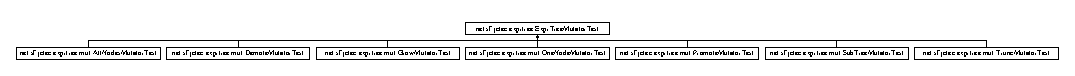
\includegraphics[height=0.571429cm]{classnet_1_1sf_1_1jclec_1_1exprtree_1_1_expr_tree_mutator_test}
\end{center}
\end{figure}
\subsection*{Public Member Functions}
\begin{DoxyCompactItemize}
\item 
\hyperlink{classnet_1_1sf_1_1jclec_1_1exprtree_1_1_expr_tree_mutator_test_a8357fb3ebe49293af2ef9c7444283329}{Expr\-Tree\-Mutator\-Test} (String name)
\end{DoxyCompactItemize}


\subsection{Detailed Description}
\hyperlink{classnet_1_1sf_1_1jclec_1_1exprtree_1_1_expr_tree_mutator}{Expr\-Tree\-Mutator} tests.

\begin{DoxyAuthor}{Author}
Amelia Zafra 

Sebastian Ventura 
\end{DoxyAuthor}


\subsection{Constructor \& Destructor Documentation}
\hypertarget{classnet_1_1sf_1_1jclec_1_1exprtree_1_1_expr_tree_mutator_test_a8357fb3ebe49293af2ef9c7444283329}{\index{net\-::sf\-::jclec\-::exprtree\-::\-Expr\-Tree\-Mutator\-Test@{net\-::sf\-::jclec\-::exprtree\-::\-Expr\-Tree\-Mutator\-Test}!Expr\-Tree\-Mutator\-Test@{Expr\-Tree\-Mutator\-Test}}
\index{Expr\-Tree\-Mutator\-Test@{Expr\-Tree\-Mutator\-Test}!net::sf::jclec::exprtree::ExprTreeMutatorTest@{net\-::sf\-::jclec\-::exprtree\-::\-Expr\-Tree\-Mutator\-Test}}
\subsubsection[{Expr\-Tree\-Mutator\-Test}]{\setlength{\rightskip}{0pt plus 5cm}net.\-sf.\-jclec.\-exprtree.\-Expr\-Tree\-Mutator\-Test.\-Expr\-Tree\-Mutator\-Test (
\begin{DoxyParamCaption}
\item[{String}]{name}
\end{DoxyParamCaption}
)}}\label{classnet_1_1sf_1_1jclec_1_1exprtree_1_1_expr_tree_mutator_test_a8357fb3ebe49293af2ef9c7444283329}
Default constructor. 

The documentation for this class was generated from the following file\-:\begin{DoxyCompactItemize}
\item 
src/test/java/net/sf/jclec/exprtree/Expr\-Tree\-Mutator\-Test.\-java\end{DoxyCompactItemize}

\hypertarget{classnet_1_1sf_1_1jclec_1_1exprtree_1_1_expr_tree_recombinator}{\section{net.\-sf.\-jclec.\-exprtree.\-Expr\-Tree\-Recombinator Class Reference}
\label{classnet_1_1sf_1_1jclec_1_1exprtree_1_1_expr_tree_recombinator}\index{net.\-sf.\-jclec.\-exprtree.\-Expr\-Tree\-Recombinator@{net.\-sf.\-jclec.\-exprtree.\-Expr\-Tree\-Recombinator}}
}
Inheritance diagram for net.\-sf.\-jclec.\-exprtree.\-Expr\-Tree\-Recombinator\-:\begin{figure}[H]
\begin{center}
\leavevmode
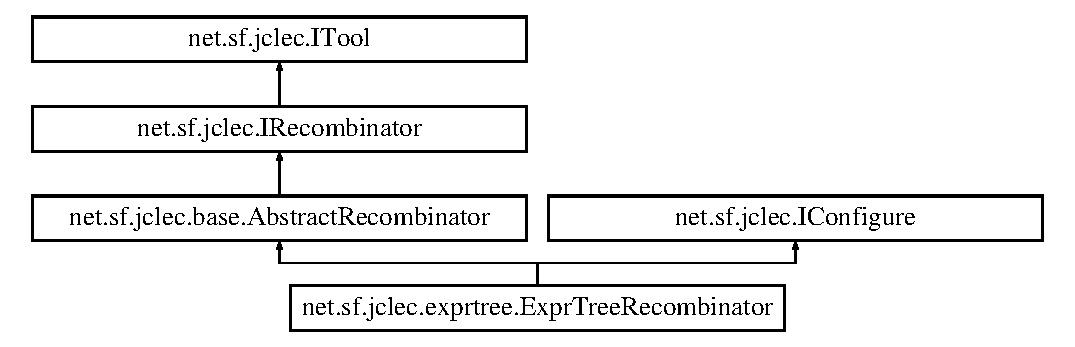
\includegraphics[height=4.000000cm]{classnet_1_1sf_1_1jclec_1_1exprtree_1_1_expr_tree_recombinator}
\end{center}
\end{figure}
\subsection*{Public Member Functions}
\begin{DoxyCompactItemize}
\item 
\hyperlink{classnet_1_1sf_1_1jclec_1_1exprtree_1_1_expr_tree_recombinator_a26d03859a1a71be818d81eb0ed95554f}{Expr\-Tree\-Recombinator} ()
\item 
void \hyperlink{classnet_1_1sf_1_1jclec_1_1exprtree_1_1_expr_tree_recombinator_a665845477525ccf265a2e8bf147de695}{configure} (Configuration settings)
\end{DoxyCompactItemize}
\subsection*{Protected Member Functions}
\begin{DoxyCompactItemize}
\item 
void \hyperlink{classnet_1_1sf_1_1jclec_1_1exprtree_1_1_expr_tree_recombinator_aa093b329ea2bb0c113b5b8c48107452b}{set\-Ppl} ()
\item 
void \hyperlink{classnet_1_1sf_1_1jclec_1_1exprtree_1_1_expr_tree_recombinator_adcd6c3e1629ec2aca0c27d43587c9ddf}{set\-Spl} ()
\item 
void \hyperlink{classnet_1_1sf_1_1jclec_1_1exprtree_1_1_expr_tree_recombinator_a19632d02d287f5e08768c824695df2ac}{prepare\-Recombination} ()
\item 
void \hyperlink{classnet_1_1sf_1_1jclec_1_1exprtree_1_1_expr_tree_recombinator_adf91b5652ebb30517f565948828adfab}{recombine\-Next} ()
\end{DoxyCompactItemize}
\subsection*{Protected Attributes}
\begin{DoxyCompactItemize}
\item 
\hyperlink{interfacenet_1_1sf_1_1jclec_1_1exprtree_1_1_i_recombine_expr_tree}{I\-Recombine\-Expr\-Tree} \hyperlink{classnet_1_1sf_1_1jclec_1_1exprtree_1_1_expr_tree_recombinator_ad70aa987e25652b6bdde419e9cbdf05d}{base\-Op}
\item 
transient \hyperlink{classnet_1_1sf_1_1jclec_1_1exprtree_1_1_expr_tree_species}{Expr\-Tree\-Species} \hyperlink{classnet_1_1sf_1_1jclec_1_1exprtree_1_1_expr_tree_recombinator_a5b2361b34daef53864f4c0486835f5b6}{species}
\item 
transient \hyperlink{classnet_1_1sf_1_1jclec_1_1exprtree_1_1_expr_tree_schema}{Expr\-Tree\-Schema} \hyperlink{classnet_1_1sf_1_1jclec_1_1exprtree_1_1_expr_tree_recombinator_a4702677649a2ad046c72d84bd6a091f7}{schema}
\end{DoxyCompactItemize}


\subsection{Detailed Description}
Recombinator for \hyperlink{classnet_1_1sf_1_1jclec_1_1exprtree_1_1_expr_tree_individual}{Expr\-Tree\-Individual} (and its subclasses).

\begin{DoxyAuthor}{Author}
Sebastian Ventura 
\end{DoxyAuthor}


\subsection{Constructor \& Destructor Documentation}
\hypertarget{classnet_1_1sf_1_1jclec_1_1exprtree_1_1_expr_tree_recombinator_a26d03859a1a71be818d81eb0ed95554f}{\index{net\-::sf\-::jclec\-::exprtree\-::\-Expr\-Tree\-Recombinator@{net\-::sf\-::jclec\-::exprtree\-::\-Expr\-Tree\-Recombinator}!Expr\-Tree\-Recombinator@{Expr\-Tree\-Recombinator}}
\index{Expr\-Tree\-Recombinator@{Expr\-Tree\-Recombinator}!net::sf::jclec::exprtree::ExprTreeRecombinator@{net\-::sf\-::jclec\-::exprtree\-::\-Expr\-Tree\-Recombinator}}
\subsubsection[{Expr\-Tree\-Recombinator}]{\setlength{\rightskip}{0pt plus 5cm}net.\-sf.\-jclec.\-exprtree.\-Expr\-Tree\-Recombinator.\-Expr\-Tree\-Recombinator (
\begin{DoxyParamCaption}
{}
\end{DoxyParamCaption}
)}}\label{classnet_1_1sf_1_1jclec_1_1exprtree_1_1_expr_tree_recombinator_a26d03859a1a71be818d81eb0ed95554f}
Empty constructor 

\subsection{Member Function Documentation}
\hypertarget{classnet_1_1sf_1_1jclec_1_1exprtree_1_1_expr_tree_recombinator_a665845477525ccf265a2e8bf147de695}{\index{net\-::sf\-::jclec\-::exprtree\-::\-Expr\-Tree\-Recombinator@{net\-::sf\-::jclec\-::exprtree\-::\-Expr\-Tree\-Recombinator}!configure@{configure}}
\index{configure@{configure}!net::sf::jclec::exprtree::ExprTreeRecombinator@{net\-::sf\-::jclec\-::exprtree\-::\-Expr\-Tree\-Recombinator}}
\subsubsection[{configure}]{\setlength{\rightskip}{0pt plus 5cm}void net.\-sf.\-jclec.\-exprtree.\-Expr\-Tree\-Recombinator.\-configure (
\begin{DoxyParamCaption}
\item[{Configuration}]{settings}
\end{DoxyParamCaption}
)}}\label{classnet_1_1sf_1_1jclec_1_1exprtree_1_1_expr_tree_recombinator_a665845477525ccf265a2e8bf147de695}
Configuration method.


\begin{DoxyParams}{Parameters}
{\em settings} & Configuration settings \\
\hline
\end{DoxyParams}


Implements \hyperlink{interfacenet_1_1sf_1_1jclec_1_1_i_configure_add31a65a04d148c690a956fbbad6987c}{net.\-sf.\-jclec.\-I\-Configure}.

\hypertarget{classnet_1_1sf_1_1jclec_1_1exprtree_1_1_expr_tree_recombinator_a19632d02d287f5e08768c824695df2ac}{\index{net\-::sf\-::jclec\-::exprtree\-::\-Expr\-Tree\-Recombinator@{net\-::sf\-::jclec\-::exprtree\-::\-Expr\-Tree\-Recombinator}!prepare\-Recombination@{prepare\-Recombination}}
\index{prepare\-Recombination@{prepare\-Recombination}!net::sf::jclec::exprtree::ExprTreeRecombinator@{net\-::sf\-::jclec\-::exprtree\-::\-Expr\-Tree\-Recombinator}}
\subsubsection[{prepare\-Recombination}]{\setlength{\rightskip}{0pt plus 5cm}void net.\-sf.\-jclec.\-exprtree.\-Expr\-Tree\-Recombinator.\-prepare\-Recombination (
\begin{DoxyParamCaption}
{}
\end{DoxyParamCaption}
)\hspace{0.3cm}{\ttfamily [protected]}, {\ttfamily [virtual]}}}\label{classnet_1_1sf_1_1jclec_1_1exprtree_1_1_expr_tree_recombinator_a19632d02d287f5e08768c824695df2ac}
Prepare recombination process. 

Implements \hyperlink{classnet_1_1sf_1_1jclec_1_1base_1_1_abstract_recombinator_ad9518cc41f28166465c4b8dc60059048}{net.\-sf.\-jclec.\-base.\-Abstract\-Recombinator}.

\hypertarget{classnet_1_1sf_1_1jclec_1_1exprtree_1_1_expr_tree_recombinator_adf91b5652ebb30517f565948828adfab}{\index{net\-::sf\-::jclec\-::exprtree\-::\-Expr\-Tree\-Recombinator@{net\-::sf\-::jclec\-::exprtree\-::\-Expr\-Tree\-Recombinator}!recombine\-Next@{recombine\-Next}}
\index{recombine\-Next@{recombine\-Next}!net::sf::jclec::exprtree::ExprTreeRecombinator@{net\-::sf\-::jclec\-::exprtree\-::\-Expr\-Tree\-Recombinator}}
\subsubsection[{recombine\-Next}]{\setlength{\rightskip}{0pt plus 5cm}void net.\-sf.\-jclec.\-exprtree.\-Expr\-Tree\-Recombinator.\-recombine\-Next (
\begin{DoxyParamCaption}
{}
\end{DoxyParamCaption}
)\hspace{0.3cm}{\ttfamily [protected]}, {\ttfamily [virtual]}}}\label{classnet_1_1sf_1_1jclec_1_1exprtree_1_1_expr_tree_recombinator_adf91b5652ebb30517f565948828adfab}
Atomic recombination method. This method ... 

Implements \hyperlink{classnet_1_1sf_1_1jclec_1_1base_1_1_abstract_recombinator_a1f94790294ad036473b5e1ffa563597e}{net.\-sf.\-jclec.\-base.\-Abstract\-Recombinator}.

\hypertarget{classnet_1_1sf_1_1jclec_1_1exprtree_1_1_expr_tree_recombinator_aa093b329ea2bb0c113b5b8c48107452b}{\index{net\-::sf\-::jclec\-::exprtree\-::\-Expr\-Tree\-Recombinator@{net\-::sf\-::jclec\-::exprtree\-::\-Expr\-Tree\-Recombinator}!set\-Ppl@{set\-Ppl}}
\index{set\-Ppl@{set\-Ppl}!net::sf::jclec::exprtree::ExprTreeRecombinator@{net\-::sf\-::jclec\-::exprtree\-::\-Expr\-Tree\-Recombinator}}
\subsubsection[{set\-Ppl}]{\setlength{\rightskip}{0pt plus 5cm}void net.\-sf.\-jclec.\-exprtree.\-Expr\-Tree\-Recombinator.\-set\-Ppl (
\begin{DoxyParamCaption}
{}
\end{DoxyParamCaption}
)\hspace{0.3cm}{\ttfamily [protected]}, {\ttfamily [virtual]}}}\label{classnet_1_1sf_1_1jclec_1_1exprtree_1_1_expr_tree_recombinator_aa093b329ea2bb0c113b5b8c48107452b}
Sets the ppl parameter (that represents the number of parents per litter). 

Implements \hyperlink{classnet_1_1sf_1_1jclec_1_1base_1_1_abstract_recombinator_aa90f858c27f9da69b2f7bb0a9220ed4e}{net.\-sf.\-jclec.\-base.\-Abstract\-Recombinator}.

\hypertarget{classnet_1_1sf_1_1jclec_1_1exprtree_1_1_expr_tree_recombinator_adcd6c3e1629ec2aca0c27d43587c9ddf}{\index{net\-::sf\-::jclec\-::exprtree\-::\-Expr\-Tree\-Recombinator@{net\-::sf\-::jclec\-::exprtree\-::\-Expr\-Tree\-Recombinator}!set\-Spl@{set\-Spl}}
\index{set\-Spl@{set\-Spl}!net::sf::jclec::exprtree::ExprTreeRecombinator@{net\-::sf\-::jclec\-::exprtree\-::\-Expr\-Tree\-Recombinator}}
\subsubsection[{set\-Spl}]{\setlength{\rightskip}{0pt plus 5cm}void net.\-sf.\-jclec.\-exprtree.\-Expr\-Tree\-Recombinator.\-set\-Spl (
\begin{DoxyParamCaption}
{}
\end{DoxyParamCaption}
)\hspace{0.3cm}{\ttfamily [protected]}, {\ttfamily [virtual]}}}\label{classnet_1_1sf_1_1jclec_1_1exprtree_1_1_expr_tree_recombinator_adcd6c3e1629ec2aca0c27d43587c9ddf}
Sets the spl parameter (that represents the number of sons per litter). 

Implements \hyperlink{classnet_1_1sf_1_1jclec_1_1base_1_1_abstract_recombinator_a49a445f27d777d6f439d97d61f2e1729}{net.\-sf.\-jclec.\-base.\-Abstract\-Recombinator}.



\subsection{Member Data Documentation}
\hypertarget{classnet_1_1sf_1_1jclec_1_1exprtree_1_1_expr_tree_recombinator_ad70aa987e25652b6bdde419e9cbdf05d}{\index{net\-::sf\-::jclec\-::exprtree\-::\-Expr\-Tree\-Recombinator@{net\-::sf\-::jclec\-::exprtree\-::\-Expr\-Tree\-Recombinator}!base\-Op@{base\-Op}}
\index{base\-Op@{base\-Op}!net::sf::jclec::exprtree::ExprTreeRecombinator@{net\-::sf\-::jclec\-::exprtree\-::\-Expr\-Tree\-Recombinator}}
\subsubsection[{base\-Op}]{\setlength{\rightskip}{0pt plus 5cm}{\bf I\-Recombine\-Expr\-Tree} net.\-sf.\-jclec.\-exprtree.\-Expr\-Tree\-Recombinator.\-base\-Op\hspace{0.3cm}{\ttfamily [protected]}}}\label{classnet_1_1sf_1_1jclec_1_1exprtree_1_1_expr_tree_recombinator_ad70aa987e25652b6bdde419e9cbdf05d}
Base operation for this expression tree mutator \hypertarget{classnet_1_1sf_1_1jclec_1_1exprtree_1_1_expr_tree_recombinator_a4702677649a2ad046c72d84bd6a091f7}{\index{net\-::sf\-::jclec\-::exprtree\-::\-Expr\-Tree\-Recombinator@{net\-::sf\-::jclec\-::exprtree\-::\-Expr\-Tree\-Recombinator}!schema@{schema}}
\index{schema@{schema}!net::sf::jclec::exprtree::ExprTreeRecombinator@{net\-::sf\-::jclec\-::exprtree\-::\-Expr\-Tree\-Recombinator}}
\subsubsection[{schema}]{\setlength{\rightskip}{0pt plus 5cm}transient {\bf Expr\-Tree\-Schema} net.\-sf.\-jclec.\-exprtree.\-Expr\-Tree\-Recombinator.\-schema\hspace{0.3cm}{\ttfamily [protected]}}}\label{classnet_1_1sf_1_1jclec_1_1exprtree_1_1_expr_tree_recombinator_a4702677649a2ad046c72d84bd6a091f7}
Individuals schema \hypertarget{classnet_1_1sf_1_1jclec_1_1exprtree_1_1_expr_tree_recombinator_a5b2361b34daef53864f4c0486835f5b6}{\index{net\-::sf\-::jclec\-::exprtree\-::\-Expr\-Tree\-Recombinator@{net\-::sf\-::jclec\-::exprtree\-::\-Expr\-Tree\-Recombinator}!species@{species}}
\index{species@{species}!net::sf::jclec::exprtree::ExprTreeRecombinator@{net\-::sf\-::jclec\-::exprtree\-::\-Expr\-Tree\-Recombinator}}
\subsubsection[{species}]{\setlength{\rightskip}{0pt plus 5cm}transient {\bf Expr\-Tree\-Species} net.\-sf.\-jclec.\-exprtree.\-Expr\-Tree\-Recombinator.\-species\hspace{0.3cm}{\ttfamily [protected]}}}\label{classnet_1_1sf_1_1jclec_1_1exprtree_1_1_expr_tree_recombinator_a5b2361b34daef53864f4c0486835f5b6}
Individual species 

The documentation for this class was generated from the following file\-:\begin{DoxyCompactItemize}
\item 
src/main/java/net/sf/jclec/exprtree/Expr\-Tree\-Recombinator.\-java\end{DoxyCompactItemize}

\hypertarget{classnet_1_1sf_1_1jclec_1_1exprtree_1_1_expr_tree_recombinator_test}{\section{net.\-sf.\-jclec.\-exprtree.\-Expr\-Tree\-Recombinator\-Test Class Reference}
\label{classnet_1_1sf_1_1jclec_1_1exprtree_1_1_expr_tree_recombinator_test}\index{net.\-sf.\-jclec.\-exprtree.\-Expr\-Tree\-Recombinator\-Test@{net.\-sf.\-jclec.\-exprtree.\-Expr\-Tree\-Recombinator\-Test}}
}


Inherits I\-Recombinator\-Test$<$ Expr\-Tree\-Recombinator $>$.



Inherited by net.\-sf.\-jclec.\-exprtree.\-rec.\-Subtree\-Crossover\-Test, and net.\-sf.\-jclec.\-exprtree.\-rec.\-Tree\-Crossover\-Test.

\subsection*{Public Member Functions}
\begin{DoxyCompactItemize}
\item 
\hyperlink{classnet_1_1sf_1_1jclec_1_1exprtree_1_1_expr_tree_recombinator_test_a4edb88503edd4f56b5d9c51e913e0889}{Expr\-Tree\-Recombinator\-Test} (String name)
\end{DoxyCompactItemize}


\subsection{Detailed Description}
\hyperlink{classnet_1_1sf_1_1jclec_1_1exprtree_1_1_expr_tree_recombinator}{Expr\-Tree\-Recombinator} tests.

\begin{DoxyAuthor}{Author}
Sebastian Ventura 
\end{DoxyAuthor}


\subsection{Constructor \& Destructor Documentation}
\hypertarget{classnet_1_1sf_1_1jclec_1_1exprtree_1_1_expr_tree_recombinator_test_a4edb88503edd4f56b5d9c51e913e0889}{\index{net\-::sf\-::jclec\-::exprtree\-::\-Expr\-Tree\-Recombinator\-Test@{net\-::sf\-::jclec\-::exprtree\-::\-Expr\-Tree\-Recombinator\-Test}!Expr\-Tree\-Recombinator\-Test@{Expr\-Tree\-Recombinator\-Test}}
\index{Expr\-Tree\-Recombinator\-Test@{Expr\-Tree\-Recombinator\-Test}!net::sf::jclec::exprtree::ExprTreeRecombinatorTest@{net\-::sf\-::jclec\-::exprtree\-::\-Expr\-Tree\-Recombinator\-Test}}
\subsubsection[{Expr\-Tree\-Recombinator\-Test}]{\setlength{\rightskip}{0pt plus 5cm}net.\-sf.\-jclec.\-exprtree.\-Expr\-Tree\-Recombinator\-Test.\-Expr\-Tree\-Recombinator\-Test (
\begin{DoxyParamCaption}
\item[{String}]{name}
\end{DoxyParamCaption}
)}}\label{classnet_1_1sf_1_1jclec_1_1exprtree_1_1_expr_tree_recombinator_test_a4edb88503edd4f56b5d9c51e913e0889}
Default constructor. 

The documentation for this class was generated from the following file\-:\begin{DoxyCompactItemize}
\item 
src/test/java/net/sf/jclec/exprtree/Expr\-Tree\-Recombinator\-Test.\-java\end{DoxyCompactItemize}

\hypertarget{classnet_1_1sf_1_1jclec_1_1exprtree_1_1_expr_tree_schema}{\section{net.\-sf.\-jclec.\-exprtree.\-Expr\-Tree\-Schema Class Reference}
\label{classnet_1_1sf_1_1jclec_1_1exprtree_1_1_expr_tree_schema}\index{net.\-sf.\-jclec.\-exprtree.\-Expr\-Tree\-Schema@{net.\-sf.\-jclec.\-exprtree.\-Expr\-Tree\-Schema}}
}


Inherits net.\-sf.\-jclec.\-J\-C\-L\-E\-C.

\subsection*{Public Member Functions}
\begin{DoxyCompactItemize}
\item 
\hyperlink{interfacenet_1_1sf_1_1jclec_1_1exprtree_1_1_i_primitive}{I\-Primitive}\mbox{[}$\,$\mbox{]} \hyperlink{classnet_1_1sf_1_1jclec_1_1exprtree_1_1_expr_tree_schema_a28d6438a7b490f5864def7b37c448f0c}{get\-Terminals} ()
\item 
\hyperlink{interfacenet_1_1sf_1_1jclec_1_1exprtree_1_1_i_primitive}{I\-Primitive}\mbox{[}$\,$\mbox{]} \hyperlink{classnet_1_1sf_1_1jclec_1_1exprtree_1_1_expr_tree_schema_a7593f2b31f1c8a7806b251aa9c537655}{get\-Functions} ()
\item 
final void \hyperlink{classnet_1_1sf_1_1jclec_1_1exprtree_1_1_expr_tree_schema_aa471670fe9fe10651ddb624c3337237c}{set\-Root\-Type} (Class$<$?$>$ \hyperlink{classnet_1_1sf_1_1jclec_1_1exprtree_1_1_expr_tree_schema_a249024518906b1b72f537d5b61ea16ff}{root\-Type})
\item 
final void \hyperlink{classnet_1_1sf_1_1jclec_1_1exprtree_1_1_expr_tree_schema_a64597f416b491f7b2a1d540765c8a5b2}{set\-Min\-Tree\-Size} (int \hyperlink{classnet_1_1sf_1_1jclec_1_1exprtree_1_1_expr_tree_schema_a1ac93c0fc7bd111a376ab405ec7b8fb3}{min\-Tree\-Size})
\item 
final void \hyperlink{classnet_1_1sf_1_1jclec_1_1exprtree_1_1_expr_tree_schema_aa83a8f26b9c81bb7447cdfadd69432f3}{set\-Max\-Tree\-Size} (int \hyperlink{classnet_1_1sf_1_1jclec_1_1exprtree_1_1_expr_tree_schema_a5a222e091d9f7eaa07c7acee9b50efc1}{max\-Tree\-Size})
\item 
final void \hyperlink{classnet_1_1sf_1_1jclec_1_1exprtree_1_1_expr_tree_schema_aae23cd8acade2e2297bef23345e24b9f}{set\-Terminals} (\hyperlink{interfacenet_1_1sf_1_1jclec_1_1exprtree_1_1_i_primitive}{I\-Primitive}\mbox{[}$\,$\mbox{]} \hyperlink{classnet_1_1sf_1_1jclec_1_1exprtree_1_1_expr_tree_schema_aa60f19ae52e55d9ed07ca1089c88d65a}{terminals})
\item 
void \hyperlink{classnet_1_1sf_1_1jclec_1_1exprtree_1_1_expr_tree_schema_a08e0cc54b355195616c1b4b4fdd6b741}{set\-Functions} (\hyperlink{interfacenet_1_1sf_1_1jclec_1_1exprtree_1_1_i_primitive}{I\-Primitive}\mbox{[}$\,$\mbox{]} \hyperlink{classnet_1_1sf_1_1jclec_1_1exprtree_1_1_expr_tree_schema_aca234d53fec87216b84803146e1b23c6}{functions})
\item 
Class$<$?$>$ \hyperlink{classnet_1_1sf_1_1jclec_1_1exprtree_1_1_expr_tree_schema_ae6578b6e75101c8a9ada29d7e03b5dc5}{get\-Root\-Type} ()
\item 
int \hyperlink{classnet_1_1sf_1_1jclec_1_1exprtree_1_1_expr_tree_schema_ad49e4ffeebe1eb3c422f34b1ca538832}{get\-Min\-Tree\-Size} ()
\item 
int \hyperlink{classnet_1_1sf_1_1jclec_1_1exprtree_1_1_expr_tree_schema_a430bca305225d072c19d8d5e91e57df6}{get\-Max\-Tree\-Size} ()
\item 
int \hyperlink{classnet_1_1sf_1_1jclec_1_1exprtree_1_1_expr_tree_schema_af11961a8c6617b0f9586395214e3b598}{get\-Num\-Function\-Blocks} (Class$<$?$>$ rtype)
\item 
\hyperlink{interfacenet_1_1sf_1_1jclec_1_1exprtree_1_1_i_primitive}{I\-Primitive} \hyperlink{classnet_1_1sf_1_1jclec_1_1exprtree_1_1_expr_tree_schema_a759d602a5fdaacdf143fb1032f025f3c}{get\-Terminal\-Block} (Class$<$?$>$ rtype, \hyperlink{interfacenet_1_1sf_1_1jclec_1_1util_1_1random_1_1_i_rand_gen}{I\-Rand\-Gen} randgen)
\item 
\hyperlink{interfacenet_1_1sf_1_1jclec_1_1exprtree_1_1_i_primitive}{I\-Primitive} \hyperlink{classnet_1_1sf_1_1jclec_1_1exprtree_1_1_expr_tree_schema_a01f03482fb411f631134059614046a72}{get\-Function\-Block} (Class$<$?$>$ rtype, \hyperlink{interfacenet_1_1sf_1_1jclec_1_1util_1_1random_1_1_i_rand_gen}{I\-Rand\-Gen} randgen)
\item 
\hyperlink{interfacenet_1_1sf_1_1jclec_1_1exprtree_1_1_i_primitive}{I\-Primitive} \hyperlink{classnet_1_1sf_1_1jclec_1_1exprtree_1_1_expr_tree_schema_a4388f39f3a8afe57d292990eff11ccbf}{get\-Function\-Block} (Class$<$?$>$ rtype, \hyperlink{interfacenet_1_1sf_1_1jclec_1_1util_1_1random_1_1_i_rand_gen}{I\-Rand\-Gen} randgen, int arity)
\item 
\hyperlink{interfacenet_1_1sf_1_1jclec_1_1exprtree_1_1_i_primitive}{I\-Primitive} \hyperlink{classnet_1_1sf_1_1jclec_1_1exprtree_1_1_expr_tree_schema_a83ca8d577369144608f7c63b7ab7e00f}{get\-Function\-Block\-Between\-Min\-Max\-Arity} (Class$<$?$>$ rtype, \hyperlink{interfacenet_1_1sf_1_1jclec_1_1util_1_1random_1_1_i_rand_gen}{I\-Rand\-Gen} randgen, int min\-Arity, int max\-Arity)
\item 
\hyperlink{interfacenet_1_1sf_1_1jclec_1_1exprtree_1_1_i_primitive}{I\-Primitive} \hyperlink{classnet_1_1sf_1_1jclec_1_1exprtree_1_1_expr_tree_schema_aa1dd1be15d247f1433d9ee9efa69ec5e}{get\-Any\-Block} (Class$<$?$>$ rtype, \hyperlink{interfacenet_1_1sf_1_1jclec_1_1util_1_1random_1_1_i_rand_gen}{I\-Rand\-Gen} randgen)
\item 
\hyperlink{interfacenet_1_1sf_1_1jclec_1_1exprtree_1_1_i_primitive}{I\-Primitive} \hyperlink{classnet_1_1sf_1_1jclec_1_1exprtree_1_1_expr_tree_schema_acd7543c47aa831b8c5ef788fa986966c}{get\-Any\-Block} (Class$<$?$>$ rtype, \hyperlink{interfacenet_1_1sf_1_1jclec_1_1util_1_1random_1_1_i_rand_gen}{I\-Rand\-Gen} randgen, int arity)
\item 
\hyperlink{classnet_1_1sf_1_1jclec_1_1exprtree_1_1_expr_tree}{Expr\-Tree} \hyperlink{classnet_1_1sf_1_1jclec_1_1exprtree_1_1_expr_tree_schema_ac6746feb1a9f6a9f42732f2b3c73660f}{create\-Expr\-Tree} (int max\-Size, \hyperlink{interfacenet_1_1sf_1_1jclec_1_1util_1_1random_1_1_i_rand_gen}{I\-Rand\-Gen} randgen)
\item 
void \hyperlink{classnet_1_1sf_1_1jclec_1_1exprtree_1_1_expr_tree_schema_a77806eaca70bdd4913227aea16b61d1a}{fill\-Expr\-Branch} (\hyperlink{classnet_1_1sf_1_1jclec_1_1exprtree_1_1_expr_tree}{Expr\-Tree} expr\-Tree, Class$<$?$>$ return\-Type, int max\-Size, \hyperlink{interfacenet_1_1sf_1_1jclec_1_1util_1_1random_1_1_i_rand_gen}{I\-Rand\-Gen} randgen)
\item 
boolean \hyperlink{classnet_1_1sf_1_1jclec_1_1exprtree_1_1_expr_tree_schema_a05be85ca80f0ad730d8ac61827035378}{equals} (Object other)
\end{DoxyCompactItemize}
\subsection*{Protected Member Functions}
\begin{DoxyCompactItemize}
\item 
final void \hyperlink{classnet_1_1sf_1_1jclec_1_1exprtree_1_1_expr_tree_schema_a2022206293d7330f674d952255ff3867}{generate\-Block\-Maps} ()
\end{DoxyCompactItemize}
\subsection*{Protected Attributes}
\begin{DoxyCompactItemize}
\item 
int \hyperlink{classnet_1_1sf_1_1jclec_1_1exprtree_1_1_expr_tree_schema_a1ac93c0fc7bd111a376ab405ec7b8fb3}{min\-Tree\-Size}
\item 
int \hyperlink{classnet_1_1sf_1_1jclec_1_1exprtree_1_1_expr_tree_schema_a5a222e091d9f7eaa07c7acee9b50efc1}{max\-Tree\-Size}
\item 
Class$<$?$>$ \hyperlink{classnet_1_1sf_1_1jclec_1_1exprtree_1_1_expr_tree_schema_a249024518906b1b72f537d5b61ea16ff}{root\-Type}
\item 
\hyperlink{interfacenet_1_1sf_1_1jclec_1_1exprtree_1_1_i_primitive}{I\-Primitive}\mbox{[}$\,$\mbox{]} \hyperlink{classnet_1_1sf_1_1jclec_1_1exprtree_1_1_expr_tree_schema_aa60f19ae52e55d9ed07ca1089c88d65a}{terminals}
\item 
\hyperlink{interfacenet_1_1sf_1_1jclec_1_1exprtree_1_1_i_primitive}{I\-Primitive}\mbox{[}$\,$\mbox{]} \hyperlink{classnet_1_1sf_1_1jclec_1_1exprtree_1_1_expr_tree_schema_aca234d53fec87216b84803146e1b23c6}{functions}
\item 
Hash\-Map$<$ Class$<$?$>$, \hyperlink{interfacenet_1_1sf_1_1jclec_1_1exprtree_1_1_i_primitive}{I\-Primitive}\mbox{[}$\,$\mbox{]}$>$ \hyperlink{classnet_1_1sf_1_1jclec_1_1exprtree_1_1_expr_tree_schema_a5b9a3597e40853603084bd67a4b5a09d}{all\-Map}
\item 
Hash\-Map$<$ Class$<$?$>$, \hyperlink{interfacenet_1_1sf_1_1jclec_1_1exprtree_1_1_i_primitive}{I\-Primitive}\mbox{[}$\,$\mbox{]}$>$ \hyperlink{classnet_1_1sf_1_1jclec_1_1exprtree_1_1_expr_tree_schema_acef767f8d25191e8d2fa6ef1c9bf5ae4}{term\-Map}
\item 
Hash\-Map$<$ Class$<$?$>$, \hyperlink{interfacenet_1_1sf_1_1jclec_1_1exprtree_1_1_i_primitive}{I\-Primitive}\mbox{[}$\,$\mbox{]}$>$ \hyperlink{classnet_1_1sf_1_1jclec_1_1exprtree_1_1_expr_tree_schema_aadf3e30ac3d79e7b5dfae0e0caf7d658}{func\-Map}
\end{DoxyCompactItemize}


\subsection{Detailed Description}
Structural information about Expr\-Trees.

\begin{DoxyAuthor}{Author}
Sebastian Ventura 
\end{DoxyAuthor}


\subsection{Member Function Documentation}
\hypertarget{classnet_1_1sf_1_1jclec_1_1exprtree_1_1_expr_tree_schema_ac6746feb1a9f6a9f42732f2b3c73660f}{\index{net\-::sf\-::jclec\-::exprtree\-::\-Expr\-Tree\-Schema@{net\-::sf\-::jclec\-::exprtree\-::\-Expr\-Tree\-Schema}!create\-Expr\-Tree@{create\-Expr\-Tree}}
\index{create\-Expr\-Tree@{create\-Expr\-Tree}!net::sf::jclec::exprtree::ExprTreeSchema@{net\-::sf\-::jclec\-::exprtree\-::\-Expr\-Tree\-Schema}}
\subsubsection[{create\-Expr\-Tree}]{\setlength{\rightskip}{0pt plus 5cm}{\bf Expr\-Tree} net.\-sf.\-jclec.\-exprtree.\-Expr\-Tree\-Schema.\-create\-Expr\-Tree (
\begin{DoxyParamCaption}
\item[{int}]{max\-Size, }
\item[{{\bf I\-Rand\-Gen}}]{randgen}
\end{DoxyParamCaption}
)}}\label{classnet_1_1sf_1_1jclec_1_1exprtree_1_1_expr_tree_schema_ac6746feb1a9f6a9f42732f2b3c73660f}
Expression tree creation.


\begin{DoxyParams}{Parameters}
{\em max\-Size} & Maximum tree size \\
\hline
{\em randgen} & Random generator\\
\hline
\end{DoxyParams}
\begin{DoxyReturn}{Returns}
A new expression tree object... 
\end{DoxyReturn}
\hypertarget{classnet_1_1sf_1_1jclec_1_1exprtree_1_1_expr_tree_schema_a05be85ca80f0ad730d8ac61827035378}{\index{net\-::sf\-::jclec\-::exprtree\-::\-Expr\-Tree\-Schema@{net\-::sf\-::jclec\-::exprtree\-::\-Expr\-Tree\-Schema}!equals@{equals}}
\index{equals@{equals}!net::sf::jclec::exprtree::ExprTreeSchema@{net\-::sf\-::jclec\-::exprtree\-::\-Expr\-Tree\-Schema}}
\subsubsection[{equals}]{\setlength{\rightskip}{0pt plus 5cm}boolean net.\-sf.\-jclec.\-exprtree.\-Expr\-Tree\-Schema.\-equals (
\begin{DoxyParamCaption}
\item[{Object}]{other}
\end{DoxyParamCaption}
)}}\label{classnet_1_1sf_1_1jclec_1_1exprtree_1_1_expr_tree_schema_a05be85ca80f0ad730d8ac61827035378}
\hypertarget{classnet_1_1sf_1_1jclec_1_1exprtree_1_1_expr_tree_schema_a77806eaca70bdd4913227aea16b61d1a}{\index{net\-::sf\-::jclec\-::exprtree\-::\-Expr\-Tree\-Schema@{net\-::sf\-::jclec\-::exprtree\-::\-Expr\-Tree\-Schema}!fill\-Expr\-Branch@{fill\-Expr\-Branch}}
\index{fill\-Expr\-Branch@{fill\-Expr\-Branch}!net::sf::jclec::exprtree::ExprTreeSchema@{net\-::sf\-::jclec\-::exprtree\-::\-Expr\-Tree\-Schema}}
\subsubsection[{fill\-Expr\-Branch}]{\setlength{\rightskip}{0pt plus 5cm}void net.\-sf.\-jclec.\-exprtree.\-Expr\-Tree\-Schema.\-fill\-Expr\-Branch (
\begin{DoxyParamCaption}
\item[{{\bf Expr\-Tree}}]{expr\-Tree, }
\item[{Class$<$?$>$}]{return\-Type, }
\item[{int}]{max\-Size, }
\item[{{\bf I\-Rand\-Gen}}]{randgen}
\end{DoxyParamCaption}
)}}\label{classnet_1_1sf_1_1jclec_1_1exprtree_1_1_expr_tree_schema_a77806eaca70bdd4913227aea16b61d1a}
Create a brach randomly, putting it in the expression tree passed as argument.


\begin{DoxyParams}{Parameters}
{\em expr\-Tree} & Tree that contains this branch \\
\hline
{\em return\-Type} & Return type for this branch \\
\hline
{\em max\-Size} & Brach size \\
\hline
{\em randgen} & Random generator used \\
\hline
\end{DoxyParams}
\hypertarget{classnet_1_1sf_1_1jclec_1_1exprtree_1_1_expr_tree_schema_a2022206293d7330f674d952255ff3867}{\index{net\-::sf\-::jclec\-::exprtree\-::\-Expr\-Tree\-Schema@{net\-::sf\-::jclec\-::exprtree\-::\-Expr\-Tree\-Schema}!generate\-Block\-Maps@{generate\-Block\-Maps}}
\index{generate\-Block\-Maps@{generate\-Block\-Maps}!net::sf::jclec::exprtree::ExprTreeSchema@{net\-::sf\-::jclec\-::exprtree\-::\-Expr\-Tree\-Schema}}
\subsubsection[{generate\-Block\-Maps}]{\setlength{\rightskip}{0pt plus 5cm}final void net.\-sf.\-jclec.\-exprtree.\-Expr\-Tree\-Schema.\-generate\-Block\-Maps (
\begin{DoxyParamCaption}
{}
\end{DoxyParamCaption}
)\hspace{0.3cm}{\ttfamily [protected]}}}\label{classnet_1_1sf_1_1jclec_1_1exprtree_1_1_expr_tree_schema_a2022206293d7330f674d952255ff3867}
Generate block maps. This method must be invoked after set terminal and function blocks and before call any block provision method. \hypertarget{classnet_1_1sf_1_1jclec_1_1exprtree_1_1_expr_tree_schema_aa1dd1be15d247f1433d9ee9efa69ec5e}{\index{net\-::sf\-::jclec\-::exprtree\-::\-Expr\-Tree\-Schema@{net\-::sf\-::jclec\-::exprtree\-::\-Expr\-Tree\-Schema}!get\-Any\-Block@{get\-Any\-Block}}
\index{get\-Any\-Block@{get\-Any\-Block}!net::sf::jclec::exprtree::ExprTreeSchema@{net\-::sf\-::jclec\-::exprtree\-::\-Expr\-Tree\-Schema}}
\subsubsection[{get\-Any\-Block}]{\setlength{\rightskip}{0pt plus 5cm}{\bf I\-Primitive} net.\-sf.\-jclec.\-exprtree.\-Expr\-Tree\-Schema.\-get\-Any\-Block (
\begin{DoxyParamCaption}
\item[{Class$<$?$>$}]{rtype, }
\item[{{\bf I\-Rand\-Gen}}]{randgen}
\end{DoxyParamCaption}
)}}\label{classnet_1_1sf_1_1jclec_1_1exprtree_1_1_expr_tree_schema_aa1dd1be15d247f1433d9ee9efa69ec5e}
Choose a valid block.


\begin{DoxyParams}{Parameters}
{\em rtype} & Return type for the block \\
\hline
{\em randgen} & Random generator used\\
\hline
\end{DoxyParams}
\begin{DoxyReturn}{Returns}
A valid function with arity from min\-Arity to max\-Arity 
\end{DoxyReturn}
\hypertarget{classnet_1_1sf_1_1jclec_1_1exprtree_1_1_expr_tree_schema_acd7543c47aa831b8c5ef788fa986966c}{\index{net\-::sf\-::jclec\-::exprtree\-::\-Expr\-Tree\-Schema@{net\-::sf\-::jclec\-::exprtree\-::\-Expr\-Tree\-Schema}!get\-Any\-Block@{get\-Any\-Block}}
\index{get\-Any\-Block@{get\-Any\-Block}!net::sf::jclec::exprtree::ExprTreeSchema@{net\-::sf\-::jclec\-::exprtree\-::\-Expr\-Tree\-Schema}}
\subsubsection[{get\-Any\-Block}]{\setlength{\rightskip}{0pt plus 5cm}{\bf I\-Primitive} net.\-sf.\-jclec.\-exprtree.\-Expr\-Tree\-Schema.\-get\-Any\-Block (
\begin{DoxyParamCaption}
\item[{Class$<$?$>$}]{rtype, }
\item[{{\bf I\-Rand\-Gen}}]{randgen, }
\item[{int}]{arity}
\end{DoxyParamCaption}
)}}\label{classnet_1_1sf_1_1jclec_1_1exprtree_1_1_expr_tree_schema_acd7543c47aa831b8c5ef788fa986966c}
Choose a valid block (with given arity).


\begin{DoxyParams}{Parameters}
{\em rtype} & Return type for the block \\
\hline
{\em randgen} & Random generator used \\
\hline
{\em arity} & Block arity\\
\hline
\end{DoxyParams}
\begin{DoxyReturn}{Returns}
A valid block for this tree 
\end{DoxyReturn}
\hypertarget{classnet_1_1sf_1_1jclec_1_1exprtree_1_1_expr_tree_schema_a01f03482fb411f631134059614046a72}{\index{net\-::sf\-::jclec\-::exprtree\-::\-Expr\-Tree\-Schema@{net\-::sf\-::jclec\-::exprtree\-::\-Expr\-Tree\-Schema}!get\-Function\-Block@{get\-Function\-Block}}
\index{get\-Function\-Block@{get\-Function\-Block}!net::sf::jclec::exprtree::ExprTreeSchema@{net\-::sf\-::jclec\-::exprtree\-::\-Expr\-Tree\-Schema}}
\subsubsection[{get\-Function\-Block}]{\setlength{\rightskip}{0pt plus 5cm}{\bf I\-Primitive} net.\-sf.\-jclec.\-exprtree.\-Expr\-Tree\-Schema.\-get\-Function\-Block (
\begin{DoxyParamCaption}
\item[{Class$<$?$>$}]{rtype, }
\item[{{\bf I\-Rand\-Gen}}]{randgen}
\end{DoxyParamCaption}
)}}\label{classnet_1_1sf_1_1jclec_1_1exprtree_1_1_expr_tree_schema_a01f03482fb411f631134059614046a72}
Choose a valid function block.


\begin{DoxyParams}{Parameters}
{\em rtype} & Return type for the block \\
\hline
{\em randgen} & Random generator used\\
\hline
\end{DoxyParams}
\begin{DoxyReturn}{Returns}
A valid block for this tree 
\end{DoxyReturn}
\hypertarget{classnet_1_1sf_1_1jclec_1_1exprtree_1_1_expr_tree_schema_a4388f39f3a8afe57d292990eff11ccbf}{\index{net\-::sf\-::jclec\-::exprtree\-::\-Expr\-Tree\-Schema@{net\-::sf\-::jclec\-::exprtree\-::\-Expr\-Tree\-Schema}!get\-Function\-Block@{get\-Function\-Block}}
\index{get\-Function\-Block@{get\-Function\-Block}!net::sf::jclec::exprtree::ExprTreeSchema@{net\-::sf\-::jclec\-::exprtree\-::\-Expr\-Tree\-Schema}}
\subsubsection[{get\-Function\-Block}]{\setlength{\rightskip}{0pt plus 5cm}{\bf I\-Primitive} net.\-sf.\-jclec.\-exprtree.\-Expr\-Tree\-Schema.\-get\-Function\-Block (
\begin{DoxyParamCaption}
\item[{Class$<$?$>$}]{rtype, }
\item[{{\bf I\-Rand\-Gen}}]{randgen, }
\item[{int}]{arity}
\end{DoxyParamCaption}
)}}\label{classnet_1_1sf_1_1jclec_1_1exprtree_1_1_expr_tree_schema_a4388f39f3a8afe57d292990eff11ccbf}
Choose a valid function block (with given arity).


\begin{DoxyParams}{Parameters}
{\em rtype} & Return type for the block \\
\hline
{\em randgen} & Random generator used \\
\hline
{\em arity} & Block arity\\
\hline
\end{DoxyParams}
\begin{DoxyReturn}{Returns}
A valid block for this tree 
\end{DoxyReturn}
\hypertarget{classnet_1_1sf_1_1jclec_1_1exprtree_1_1_expr_tree_schema_a83ca8d577369144608f7c63b7ab7e00f}{\index{net\-::sf\-::jclec\-::exprtree\-::\-Expr\-Tree\-Schema@{net\-::sf\-::jclec\-::exprtree\-::\-Expr\-Tree\-Schema}!get\-Function\-Block\-Between\-Min\-Max\-Arity@{get\-Function\-Block\-Between\-Min\-Max\-Arity}}
\index{get\-Function\-Block\-Between\-Min\-Max\-Arity@{get\-Function\-Block\-Between\-Min\-Max\-Arity}!net::sf::jclec::exprtree::ExprTreeSchema@{net\-::sf\-::jclec\-::exprtree\-::\-Expr\-Tree\-Schema}}
\subsubsection[{get\-Function\-Block\-Between\-Min\-Max\-Arity}]{\setlength{\rightskip}{0pt plus 5cm}{\bf I\-Primitive} net.\-sf.\-jclec.\-exprtree.\-Expr\-Tree\-Schema.\-get\-Function\-Block\-Between\-Min\-Max\-Arity (
\begin{DoxyParamCaption}
\item[{Class$<$?$>$}]{rtype, }
\item[{{\bf I\-Rand\-Gen}}]{randgen, }
\item[{int}]{min\-Arity, }
\item[{int}]{max\-Arity}
\end{DoxyParamCaption}
)}}\label{classnet_1_1sf_1_1jclec_1_1exprtree_1_1_expr_tree_schema_a83ca8d577369144608f7c63b7ab7e00f}
Choose a valid function block (with given arity).


\begin{DoxyParams}{Parameters}
{\em rtype} & Return type for the block \\
\hline
{\em randgen} & Random generator used \\
\hline
{\em min\-Arity} & Minimum arity \\
\hline
{\em max\-Arity} & Maximum arity\\
\hline
\end{DoxyParams}
\begin{DoxyReturn}{Returns}
A valid block for this tree 
\end{DoxyReturn}
\hypertarget{classnet_1_1sf_1_1jclec_1_1exprtree_1_1_expr_tree_schema_a7593f2b31f1c8a7806b251aa9c537655}{\index{net\-::sf\-::jclec\-::exprtree\-::\-Expr\-Tree\-Schema@{net\-::sf\-::jclec\-::exprtree\-::\-Expr\-Tree\-Schema}!get\-Functions@{get\-Functions}}
\index{get\-Functions@{get\-Functions}!net::sf::jclec::exprtree::ExprTreeSchema@{net\-::sf\-::jclec\-::exprtree\-::\-Expr\-Tree\-Schema}}
\subsubsection[{get\-Functions}]{\setlength{\rightskip}{0pt plus 5cm}{\bf I\-Primitive} \mbox{[}$\,$\mbox{]} net.\-sf.\-jclec.\-exprtree.\-Expr\-Tree\-Schema.\-get\-Functions (
\begin{DoxyParamCaption}
{}
\end{DoxyParamCaption}
)}}\label{classnet_1_1sf_1_1jclec_1_1exprtree_1_1_expr_tree_schema_a7593f2b31f1c8a7806b251aa9c537655}
\begin{DoxyReturn}{Returns}
the functions 
\end{DoxyReturn}
\hypertarget{classnet_1_1sf_1_1jclec_1_1exprtree_1_1_expr_tree_schema_a430bca305225d072c19d8d5e91e57df6}{\index{net\-::sf\-::jclec\-::exprtree\-::\-Expr\-Tree\-Schema@{net\-::sf\-::jclec\-::exprtree\-::\-Expr\-Tree\-Schema}!get\-Max\-Tree\-Size@{get\-Max\-Tree\-Size}}
\index{get\-Max\-Tree\-Size@{get\-Max\-Tree\-Size}!net::sf::jclec::exprtree::ExprTreeSchema@{net\-::sf\-::jclec\-::exprtree\-::\-Expr\-Tree\-Schema}}
\subsubsection[{get\-Max\-Tree\-Size}]{\setlength{\rightskip}{0pt plus 5cm}int net.\-sf.\-jclec.\-exprtree.\-Expr\-Tree\-Schema.\-get\-Max\-Tree\-Size (
\begin{DoxyParamCaption}
{}
\end{DoxyParamCaption}
)}}\label{classnet_1_1sf_1_1jclec_1_1exprtree_1_1_expr_tree_schema_a430bca305225d072c19d8d5e91e57df6}
Maximum tree size \hypertarget{classnet_1_1sf_1_1jclec_1_1exprtree_1_1_expr_tree_schema_ad49e4ffeebe1eb3c422f34b1ca538832}{\index{net\-::sf\-::jclec\-::exprtree\-::\-Expr\-Tree\-Schema@{net\-::sf\-::jclec\-::exprtree\-::\-Expr\-Tree\-Schema}!get\-Min\-Tree\-Size@{get\-Min\-Tree\-Size}}
\index{get\-Min\-Tree\-Size@{get\-Min\-Tree\-Size}!net::sf::jclec::exprtree::ExprTreeSchema@{net\-::sf\-::jclec\-::exprtree\-::\-Expr\-Tree\-Schema}}
\subsubsection[{get\-Min\-Tree\-Size}]{\setlength{\rightskip}{0pt plus 5cm}int net.\-sf.\-jclec.\-exprtree.\-Expr\-Tree\-Schema.\-get\-Min\-Tree\-Size (
\begin{DoxyParamCaption}
{}
\end{DoxyParamCaption}
)}}\label{classnet_1_1sf_1_1jclec_1_1exprtree_1_1_expr_tree_schema_ad49e4ffeebe1eb3c422f34b1ca538832}
Minimum tree size \hypertarget{classnet_1_1sf_1_1jclec_1_1exprtree_1_1_expr_tree_schema_af11961a8c6617b0f9586395214e3b598}{\index{net\-::sf\-::jclec\-::exprtree\-::\-Expr\-Tree\-Schema@{net\-::sf\-::jclec\-::exprtree\-::\-Expr\-Tree\-Schema}!get\-Num\-Function\-Blocks@{get\-Num\-Function\-Blocks}}
\index{get\-Num\-Function\-Blocks@{get\-Num\-Function\-Blocks}!net::sf::jclec::exprtree::ExprTreeSchema@{net\-::sf\-::jclec\-::exprtree\-::\-Expr\-Tree\-Schema}}
\subsubsection[{get\-Num\-Function\-Blocks}]{\setlength{\rightskip}{0pt plus 5cm}int net.\-sf.\-jclec.\-exprtree.\-Expr\-Tree\-Schema.\-get\-Num\-Function\-Blocks (
\begin{DoxyParamCaption}
\item[{Class$<$?$>$}]{rtype}
\end{DoxyParamCaption}
)}}\label{classnet_1_1sf_1_1jclec_1_1exprtree_1_1_expr_tree_schema_af11961a8c6617b0f9586395214e3b598}
Informs about the number of possible functions.

\begin{DoxyReturn}{Returns}
Number of function blocks 
\end{DoxyReturn}
\hypertarget{classnet_1_1sf_1_1jclec_1_1exprtree_1_1_expr_tree_schema_ae6578b6e75101c8a9ada29d7e03b5dc5}{\index{net\-::sf\-::jclec\-::exprtree\-::\-Expr\-Tree\-Schema@{net\-::sf\-::jclec\-::exprtree\-::\-Expr\-Tree\-Schema}!get\-Root\-Type@{get\-Root\-Type}}
\index{get\-Root\-Type@{get\-Root\-Type}!net::sf::jclec::exprtree::ExprTreeSchema@{net\-::sf\-::jclec\-::exprtree\-::\-Expr\-Tree\-Schema}}
\subsubsection[{get\-Root\-Type}]{\setlength{\rightskip}{0pt plus 5cm}Class$<$?$>$ net.\-sf.\-jclec.\-exprtree.\-Expr\-Tree\-Schema.\-get\-Root\-Type (
\begin{DoxyParamCaption}
{}
\end{DoxyParamCaption}
)}}\label{classnet_1_1sf_1_1jclec_1_1exprtree_1_1_expr_tree_schema_ae6578b6e75101c8a9ada29d7e03b5dc5}
Informs about the return (root) type for this expression.

\begin{DoxyReturn}{Returns}
Root (return) type 
\end{DoxyReturn}
\hypertarget{classnet_1_1sf_1_1jclec_1_1exprtree_1_1_expr_tree_schema_a759d602a5fdaacdf143fb1032f025f3c}{\index{net\-::sf\-::jclec\-::exprtree\-::\-Expr\-Tree\-Schema@{net\-::sf\-::jclec\-::exprtree\-::\-Expr\-Tree\-Schema}!get\-Terminal\-Block@{get\-Terminal\-Block}}
\index{get\-Terminal\-Block@{get\-Terminal\-Block}!net::sf::jclec::exprtree::ExprTreeSchema@{net\-::sf\-::jclec\-::exprtree\-::\-Expr\-Tree\-Schema}}
\subsubsection[{get\-Terminal\-Block}]{\setlength{\rightskip}{0pt plus 5cm}{\bf I\-Primitive} net.\-sf.\-jclec.\-exprtree.\-Expr\-Tree\-Schema.\-get\-Terminal\-Block (
\begin{DoxyParamCaption}
\item[{Class$<$?$>$}]{rtype, }
\item[{{\bf I\-Rand\-Gen}}]{randgen}
\end{DoxyParamCaption}
)}}\label{classnet_1_1sf_1_1jclec_1_1exprtree_1_1_expr_tree_schema_a759d602a5fdaacdf143fb1032f025f3c}
Choose a valid terminal block (used in full methods).


\begin{DoxyParams}{Parameters}
{\em rtype} & Return type for the block\\
\hline
\end{DoxyParams}
\begin{DoxyReturn}{Returns}
A valid block for this tree 
\end{DoxyReturn}
\hypertarget{classnet_1_1sf_1_1jclec_1_1exprtree_1_1_expr_tree_schema_a28d6438a7b490f5864def7b37c448f0c}{\index{net\-::sf\-::jclec\-::exprtree\-::\-Expr\-Tree\-Schema@{net\-::sf\-::jclec\-::exprtree\-::\-Expr\-Tree\-Schema}!get\-Terminals@{get\-Terminals}}
\index{get\-Terminals@{get\-Terminals}!net::sf::jclec::exprtree::ExprTreeSchema@{net\-::sf\-::jclec\-::exprtree\-::\-Expr\-Tree\-Schema}}
\subsubsection[{get\-Terminals}]{\setlength{\rightskip}{0pt plus 5cm}{\bf I\-Primitive} \mbox{[}$\,$\mbox{]} net.\-sf.\-jclec.\-exprtree.\-Expr\-Tree\-Schema.\-get\-Terminals (
\begin{DoxyParamCaption}
{}
\end{DoxyParamCaption}
)}}\label{classnet_1_1sf_1_1jclec_1_1exprtree_1_1_expr_tree_schema_a28d6438a7b490f5864def7b37c448f0c}
\begin{DoxyReturn}{Returns}
the terminals 
\end{DoxyReturn}
\hypertarget{classnet_1_1sf_1_1jclec_1_1exprtree_1_1_expr_tree_schema_a08e0cc54b355195616c1b4b4fdd6b741}{\index{net\-::sf\-::jclec\-::exprtree\-::\-Expr\-Tree\-Schema@{net\-::sf\-::jclec\-::exprtree\-::\-Expr\-Tree\-Schema}!set\-Functions@{set\-Functions}}
\index{set\-Functions@{set\-Functions}!net::sf::jclec::exprtree::ExprTreeSchema@{net\-::sf\-::jclec\-::exprtree\-::\-Expr\-Tree\-Schema}}
\subsubsection[{set\-Functions}]{\setlength{\rightskip}{0pt plus 5cm}void net.\-sf.\-jclec.\-exprtree.\-Expr\-Tree\-Schema.\-set\-Functions (
\begin{DoxyParamCaption}
\item[{{\bf I\-Primitive}\mbox{[}$\,$\mbox{]}}]{functions}
\end{DoxyParamCaption}
)}}\label{classnet_1_1sf_1_1jclec_1_1exprtree_1_1_expr_tree_schema_a08e0cc54b355195616c1b4b4fdd6b741}
Set the functions that can be used to build valid expression trees.


\begin{DoxyParams}{Parameters}
{\em functions} & Valid function nodes \\
\hline
\end{DoxyParams}
\hypertarget{classnet_1_1sf_1_1jclec_1_1exprtree_1_1_expr_tree_schema_aa83a8f26b9c81bb7447cdfadd69432f3}{\index{net\-::sf\-::jclec\-::exprtree\-::\-Expr\-Tree\-Schema@{net\-::sf\-::jclec\-::exprtree\-::\-Expr\-Tree\-Schema}!set\-Max\-Tree\-Size@{set\-Max\-Tree\-Size}}
\index{set\-Max\-Tree\-Size@{set\-Max\-Tree\-Size}!net::sf::jclec::exprtree::ExprTreeSchema@{net\-::sf\-::jclec\-::exprtree\-::\-Expr\-Tree\-Schema}}
\subsubsection[{set\-Max\-Tree\-Size}]{\setlength{\rightskip}{0pt plus 5cm}final void net.\-sf.\-jclec.\-exprtree.\-Expr\-Tree\-Schema.\-set\-Max\-Tree\-Size (
\begin{DoxyParamCaption}
\item[{int}]{max\-Tree\-Size}
\end{DoxyParamCaption}
)}}\label{classnet_1_1sf_1_1jclec_1_1exprtree_1_1_expr_tree_schema_aa83a8f26b9c81bb7447cdfadd69432f3}
Sets the maximum size for the expression trees represented by this schema


\begin{DoxyParams}{Parameters}
{\em max\-Tree\-Size} & Minimum tree size \\
\hline
\end{DoxyParams}
\hypertarget{classnet_1_1sf_1_1jclec_1_1exprtree_1_1_expr_tree_schema_a64597f416b491f7b2a1d540765c8a5b2}{\index{net\-::sf\-::jclec\-::exprtree\-::\-Expr\-Tree\-Schema@{net\-::sf\-::jclec\-::exprtree\-::\-Expr\-Tree\-Schema}!set\-Min\-Tree\-Size@{set\-Min\-Tree\-Size}}
\index{set\-Min\-Tree\-Size@{set\-Min\-Tree\-Size}!net::sf::jclec::exprtree::ExprTreeSchema@{net\-::sf\-::jclec\-::exprtree\-::\-Expr\-Tree\-Schema}}
\subsubsection[{set\-Min\-Tree\-Size}]{\setlength{\rightskip}{0pt plus 5cm}final void net.\-sf.\-jclec.\-exprtree.\-Expr\-Tree\-Schema.\-set\-Min\-Tree\-Size (
\begin{DoxyParamCaption}
\item[{int}]{min\-Tree\-Size}
\end{DoxyParamCaption}
)}}\label{classnet_1_1sf_1_1jclec_1_1exprtree_1_1_expr_tree_schema_a64597f416b491f7b2a1d540765c8a5b2}
Sets the minimum size for the expression trees represented by this schema


\begin{DoxyParams}{Parameters}
{\em min\-Tree\-Size} & Minimum tree size \\
\hline
\end{DoxyParams}
\hypertarget{classnet_1_1sf_1_1jclec_1_1exprtree_1_1_expr_tree_schema_aa471670fe9fe10651ddb624c3337237c}{\index{net\-::sf\-::jclec\-::exprtree\-::\-Expr\-Tree\-Schema@{net\-::sf\-::jclec\-::exprtree\-::\-Expr\-Tree\-Schema}!set\-Root\-Type@{set\-Root\-Type}}
\index{set\-Root\-Type@{set\-Root\-Type}!net::sf::jclec::exprtree::ExprTreeSchema@{net\-::sf\-::jclec\-::exprtree\-::\-Expr\-Tree\-Schema}}
\subsubsection[{set\-Root\-Type}]{\setlength{\rightskip}{0pt plus 5cm}final void net.\-sf.\-jclec.\-exprtree.\-Expr\-Tree\-Schema.\-set\-Root\-Type (
\begin{DoxyParamCaption}
\item[{Class$<$?$>$}]{root\-Type}
\end{DoxyParamCaption}
)}}\label{classnet_1_1sf_1_1jclec_1_1exprtree_1_1_expr_tree_schema_aa471670fe9fe10651ddb624c3337237c}
Sets the root type for the expression trees represented by this schema


\begin{DoxyParams}{Parameters}
{\em root\-Type} & Root type \\
\hline
\end{DoxyParams}
\hypertarget{classnet_1_1sf_1_1jclec_1_1exprtree_1_1_expr_tree_schema_aae23cd8acade2e2297bef23345e24b9f}{\index{net\-::sf\-::jclec\-::exprtree\-::\-Expr\-Tree\-Schema@{net\-::sf\-::jclec\-::exprtree\-::\-Expr\-Tree\-Schema}!set\-Terminals@{set\-Terminals}}
\index{set\-Terminals@{set\-Terminals}!net::sf::jclec::exprtree::ExprTreeSchema@{net\-::sf\-::jclec\-::exprtree\-::\-Expr\-Tree\-Schema}}
\subsubsection[{set\-Terminals}]{\setlength{\rightskip}{0pt plus 5cm}final void net.\-sf.\-jclec.\-exprtree.\-Expr\-Tree\-Schema.\-set\-Terminals (
\begin{DoxyParamCaption}
\item[{{\bf I\-Primitive}\mbox{[}$\,$\mbox{]}}]{terminals}
\end{DoxyParamCaption}
)}}\label{classnet_1_1sf_1_1jclec_1_1exprtree_1_1_expr_tree_schema_aae23cd8acade2e2297bef23345e24b9f}
Set the terminals that can be used to build valid expression trees.


\begin{DoxyParams}{Parameters}
{\em terminals} & Valid terminal nodes \\
\hline
\end{DoxyParams}


\subsection{Member Data Documentation}
\hypertarget{classnet_1_1sf_1_1jclec_1_1exprtree_1_1_expr_tree_schema_a5b9a3597e40853603084bd67a4b5a09d}{\index{net\-::sf\-::jclec\-::exprtree\-::\-Expr\-Tree\-Schema@{net\-::sf\-::jclec\-::exprtree\-::\-Expr\-Tree\-Schema}!all\-Map@{all\-Map}}
\index{all\-Map@{all\-Map}!net::sf::jclec::exprtree::ExprTreeSchema@{net\-::sf\-::jclec\-::exprtree\-::\-Expr\-Tree\-Schema}}
\subsubsection[{all\-Map}]{\setlength{\rightskip}{0pt plus 5cm}Hash\-Map$<$Class$<$?$>$, {\bf I\-Primitive}\mbox{[}$\,$\mbox{]}$>$ net.\-sf.\-jclec.\-exprtree.\-Expr\-Tree\-Schema.\-all\-Map\hspace{0.3cm}{\ttfamily [protected]}}}\label{classnet_1_1sf_1_1jclec_1_1exprtree_1_1_expr_tree_schema_a5b9a3597e40853603084bd67a4b5a09d}
All blocks map \hypertarget{classnet_1_1sf_1_1jclec_1_1exprtree_1_1_expr_tree_schema_aadf3e30ac3d79e7b5dfae0e0caf7d658}{\index{net\-::sf\-::jclec\-::exprtree\-::\-Expr\-Tree\-Schema@{net\-::sf\-::jclec\-::exprtree\-::\-Expr\-Tree\-Schema}!func\-Map@{func\-Map}}
\index{func\-Map@{func\-Map}!net::sf::jclec::exprtree::ExprTreeSchema@{net\-::sf\-::jclec\-::exprtree\-::\-Expr\-Tree\-Schema}}
\subsubsection[{func\-Map}]{\setlength{\rightskip}{0pt plus 5cm}Hash\-Map$<$Class$<$?$>$, {\bf I\-Primitive}\mbox{[}$\,$\mbox{]}$>$ net.\-sf.\-jclec.\-exprtree.\-Expr\-Tree\-Schema.\-func\-Map\hspace{0.3cm}{\ttfamily [protected]}}}\label{classnet_1_1sf_1_1jclec_1_1exprtree_1_1_expr_tree_schema_aadf3e30ac3d79e7b5dfae0e0caf7d658}
Function blocks map \hypertarget{classnet_1_1sf_1_1jclec_1_1exprtree_1_1_expr_tree_schema_aca234d53fec87216b84803146e1b23c6}{\index{net\-::sf\-::jclec\-::exprtree\-::\-Expr\-Tree\-Schema@{net\-::sf\-::jclec\-::exprtree\-::\-Expr\-Tree\-Schema}!functions@{functions}}
\index{functions@{functions}!net::sf::jclec::exprtree::ExprTreeSchema@{net\-::sf\-::jclec\-::exprtree\-::\-Expr\-Tree\-Schema}}
\subsubsection[{functions}]{\setlength{\rightskip}{0pt plus 5cm}{\bf I\-Primitive} \mbox{[}$\,$\mbox{]} net.\-sf.\-jclec.\-exprtree.\-Expr\-Tree\-Schema.\-functions\hspace{0.3cm}{\ttfamily [protected]}}}\label{classnet_1_1sf_1_1jclec_1_1exprtree_1_1_expr_tree_schema_aca234d53fec87216b84803146e1b23c6}
Function blocks \hypertarget{classnet_1_1sf_1_1jclec_1_1exprtree_1_1_expr_tree_schema_a5a222e091d9f7eaa07c7acee9b50efc1}{\index{net\-::sf\-::jclec\-::exprtree\-::\-Expr\-Tree\-Schema@{net\-::sf\-::jclec\-::exprtree\-::\-Expr\-Tree\-Schema}!max\-Tree\-Size@{max\-Tree\-Size}}
\index{max\-Tree\-Size@{max\-Tree\-Size}!net::sf::jclec::exprtree::ExprTreeSchema@{net\-::sf\-::jclec\-::exprtree\-::\-Expr\-Tree\-Schema}}
\subsubsection[{max\-Tree\-Size}]{\setlength{\rightskip}{0pt plus 5cm}int net.\-sf.\-jclec.\-exprtree.\-Expr\-Tree\-Schema.\-max\-Tree\-Size\hspace{0.3cm}{\ttfamily [protected]}}}\label{classnet_1_1sf_1_1jclec_1_1exprtree_1_1_expr_tree_schema_a5a222e091d9f7eaa07c7acee9b50efc1}
Maximum tree size \hypertarget{classnet_1_1sf_1_1jclec_1_1exprtree_1_1_expr_tree_schema_a1ac93c0fc7bd111a376ab405ec7b8fb3}{\index{net\-::sf\-::jclec\-::exprtree\-::\-Expr\-Tree\-Schema@{net\-::sf\-::jclec\-::exprtree\-::\-Expr\-Tree\-Schema}!min\-Tree\-Size@{min\-Tree\-Size}}
\index{min\-Tree\-Size@{min\-Tree\-Size}!net::sf::jclec::exprtree::ExprTreeSchema@{net\-::sf\-::jclec\-::exprtree\-::\-Expr\-Tree\-Schema}}
\subsubsection[{min\-Tree\-Size}]{\setlength{\rightskip}{0pt plus 5cm}int net.\-sf.\-jclec.\-exprtree.\-Expr\-Tree\-Schema.\-min\-Tree\-Size\hspace{0.3cm}{\ttfamily [protected]}}}\label{classnet_1_1sf_1_1jclec_1_1exprtree_1_1_expr_tree_schema_a1ac93c0fc7bd111a376ab405ec7b8fb3}
Minimum tree size \hypertarget{classnet_1_1sf_1_1jclec_1_1exprtree_1_1_expr_tree_schema_a249024518906b1b72f537d5b61ea16ff}{\index{net\-::sf\-::jclec\-::exprtree\-::\-Expr\-Tree\-Schema@{net\-::sf\-::jclec\-::exprtree\-::\-Expr\-Tree\-Schema}!root\-Type@{root\-Type}}
\index{root\-Type@{root\-Type}!net::sf::jclec::exprtree::ExprTreeSchema@{net\-::sf\-::jclec\-::exprtree\-::\-Expr\-Tree\-Schema}}
\subsubsection[{root\-Type}]{\setlength{\rightskip}{0pt plus 5cm}Class$<$?$>$ net.\-sf.\-jclec.\-exprtree.\-Expr\-Tree\-Schema.\-root\-Type\hspace{0.3cm}{\ttfamily [protected]}}}\label{classnet_1_1sf_1_1jclec_1_1exprtree_1_1_expr_tree_schema_a249024518906b1b72f537d5b61ea16ff}
Root type \hypertarget{classnet_1_1sf_1_1jclec_1_1exprtree_1_1_expr_tree_schema_aa60f19ae52e55d9ed07ca1089c88d65a}{\index{net\-::sf\-::jclec\-::exprtree\-::\-Expr\-Tree\-Schema@{net\-::sf\-::jclec\-::exprtree\-::\-Expr\-Tree\-Schema}!terminals@{terminals}}
\index{terminals@{terminals}!net::sf::jclec::exprtree::ExprTreeSchema@{net\-::sf\-::jclec\-::exprtree\-::\-Expr\-Tree\-Schema}}
\subsubsection[{terminals}]{\setlength{\rightskip}{0pt plus 5cm}{\bf I\-Primitive} \mbox{[}$\,$\mbox{]} net.\-sf.\-jclec.\-exprtree.\-Expr\-Tree\-Schema.\-terminals\hspace{0.3cm}{\ttfamily [protected]}}}\label{classnet_1_1sf_1_1jclec_1_1exprtree_1_1_expr_tree_schema_aa60f19ae52e55d9ed07ca1089c88d65a}
Terminal blocks \hypertarget{classnet_1_1sf_1_1jclec_1_1exprtree_1_1_expr_tree_schema_acef767f8d25191e8d2fa6ef1c9bf5ae4}{\index{net\-::sf\-::jclec\-::exprtree\-::\-Expr\-Tree\-Schema@{net\-::sf\-::jclec\-::exprtree\-::\-Expr\-Tree\-Schema}!term\-Map@{term\-Map}}
\index{term\-Map@{term\-Map}!net::sf::jclec::exprtree::ExprTreeSchema@{net\-::sf\-::jclec\-::exprtree\-::\-Expr\-Tree\-Schema}}
\subsubsection[{term\-Map}]{\setlength{\rightskip}{0pt plus 5cm}Hash\-Map$<$Class$<$?$>$, {\bf I\-Primitive}\mbox{[}$\,$\mbox{]}$>$ net.\-sf.\-jclec.\-exprtree.\-Expr\-Tree\-Schema.\-term\-Map\hspace{0.3cm}{\ttfamily [protected]}}}\label{classnet_1_1sf_1_1jclec_1_1exprtree_1_1_expr_tree_schema_acef767f8d25191e8d2fa6ef1c9bf5ae4}
Terminal blocks map 

The documentation for this class was generated from the following file\-:\begin{DoxyCompactItemize}
\item 
src/main/java/net/sf/jclec/exprtree/Expr\-Tree\-Schema.\-java\end{DoxyCompactItemize}

\hypertarget{classnet_1_1sf_1_1jclec_1_1exprtree_1_1_expr_tree_species}{\section{net.\-sf.\-jclec.\-exprtree.\-Expr\-Tree\-Species Class Reference}
\label{classnet_1_1sf_1_1jclec_1_1exprtree_1_1_expr_tree_species}\index{net.\-sf.\-jclec.\-exprtree.\-Expr\-Tree\-Species@{net.\-sf.\-jclec.\-exprtree.\-Expr\-Tree\-Species}}
}
Inheritance diagram for net.\-sf.\-jclec.\-exprtree.\-Expr\-Tree\-Species\-:\begin{figure}[H]
\begin{center}
\leavevmode
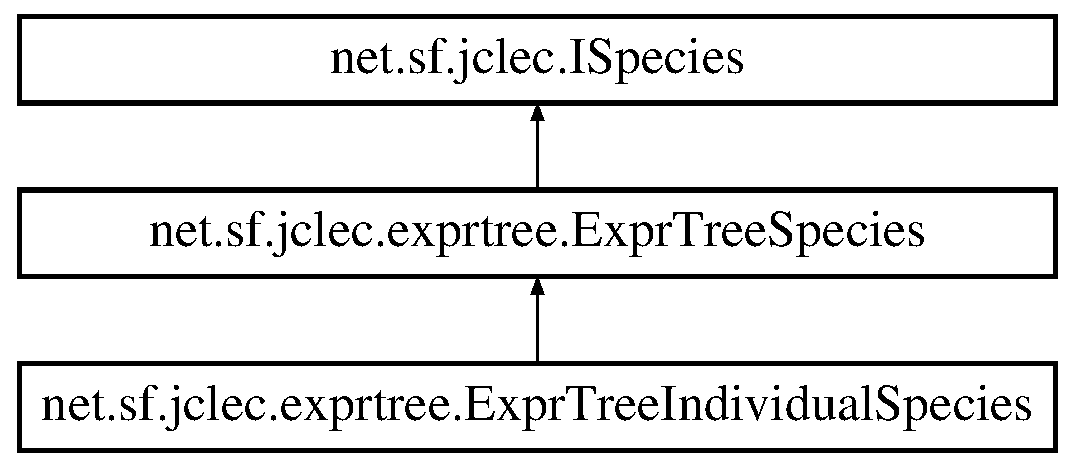
\includegraphics[height=4.000000cm]{classnet_1_1sf_1_1jclec_1_1exprtree_1_1_expr_tree_species}
\end{center}
\end{figure}
\subsection*{Public Member Functions}
\begin{DoxyCompactItemize}
\item 
\hyperlink{classnet_1_1sf_1_1jclec_1_1exprtree_1_1_expr_tree_species_a57756ad15f409b26fe51e27eaccf5905}{Expr\-Tree\-Species} ()
\item 
abstract \hyperlink{classnet_1_1sf_1_1jclec_1_1exprtree_1_1_expr_tree_individual}{Expr\-Tree\-Individual} \hyperlink{classnet_1_1sf_1_1jclec_1_1exprtree_1_1_expr_tree_species_afd641a58862d811f75a112b2dbdd9e0b}{create\-Individual} (\hyperlink{classnet_1_1sf_1_1jclec_1_1exprtree_1_1_expr_tree}{Expr\-Tree} genotype)
\item 
\hyperlink{classnet_1_1sf_1_1jclec_1_1exprtree_1_1_expr_tree_schema}{Expr\-Tree\-Schema} \hyperlink{classnet_1_1sf_1_1jclec_1_1exprtree_1_1_expr_tree_species_ae59c270bfe9783ffef96ae79fbcb0606}{get\-Genotype\-Schema} ()
\end{DoxyCompactItemize}
\subsection*{Protected Attributes}
\begin{DoxyCompactItemize}
\item 
\hyperlink{classnet_1_1sf_1_1jclec_1_1exprtree_1_1_expr_tree_schema}{Expr\-Tree\-Schema} \hyperlink{classnet_1_1sf_1_1jclec_1_1exprtree_1_1_expr_tree_species_aade758523efbdefd12889c858c7247a1}{genotype\-Schema}
\end{DoxyCompactItemize}


\subsection{Detailed Description}
I\-Expr\-Tree\-Species abstract implementation.

\begin{DoxyAuthor}{Author}
Sebastian Ventura 
\end{DoxyAuthor}


\subsection{Constructor \& Destructor Documentation}
\hypertarget{classnet_1_1sf_1_1jclec_1_1exprtree_1_1_expr_tree_species_a57756ad15f409b26fe51e27eaccf5905}{\index{net\-::sf\-::jclec\-::exprtree\-::\-Expr\-Tree\-Species@{net\-::sf\-::jclec\-::exprtree\-::\-Expr\-Tree\-Species}!Expr\-Tree\-Species@{Expr\-Tree\-Species}}
\index{Expr\-Tree\-Species@{Expr\-Tree\-Species}!net::sf::jclec::exprtree::ExprTreeSpecies@{net\-::sf\-::jclec\-::exprtree\-::\-Expr\-Tree\-Species}}
\subsubsection[{Expr\-Tree\-Species}]{\setlength{\rightskip}{0pt plus 5cm}net.\-sf.\-jclec.\-exprtree.\-Expr\-Tree\-Species.\-Expr\-Tree\-Species (
\begin{DoxyParamCaption}
{}
\end{DoxyParamCaption}
)}}\label{classnet_1_1sf_1_1jclec_1_1exprtree_1_1_expr_tree_species_a57756ad15f409b26fe51e27eaccf5905}
Empty constructor 

\subsection{Member Function Documentation}
\hypertarget{classnet_1_1sf_1_1jclec_1_1exprtree_1_1_expr_tree_species_afd641a58862d811f75a112b2dbdd9e0b}{\index{net\-::sf\-::jclec\-::exprtree\-::\-Expr\-Tree\-Species@{net\-::sf\-::jclec\-::exprtree\-::\-Expr\-Tree\-Species}!create\-Individual@{create\-Individual}}
\index{create\-Individual@{create\-Individual}!net::sf::jclec::exprtree::ExprTreeSpecies@{net\-::sf\-::jclec\-::exprtree\-::\-Expr\-Tree\-Species}}
\subsubsection[{create\-Individual}]{\setlength{\rightskip}{0pt plus 5cm}abstract {\bf Expr\-Tree\-Individual} net.\-sf.\-jclec.\-exprtree.\-Expr\-Tree\-Species.\-create\-Individual (
\begin{DoxyParamCaption}
\item[{{\bf Expr\-Tree}}]{genotype}
\end{DoxyParamCaption}
)\hspace{0.3cm}{\ttfamily [pure virtual]}}}\label{classnet_1_1sf_1_1jclec_1_1exprtree_1_1_expr_tree_species_afd641a58862d811f75a112b2dbdd9e0b}
Factory method. Set individual genotype.


\begin{DoxyParams}{Parameters}
{\em genotype} & Individual genotype\\
\hline
\end{DoxyParams}
\begin{DoxyReturn}{Returns}
A new instance of individual class, with its genotype set 
\end{DoxyReturn}


Implemented in \hyperlink{classnet_1_1sf_1_1jclec_1_1exprtree_1_1_expr_tree_individual_species_a1fb358ef3ae35458367cc916fa194884}{net.\-sf.\-jclec.\-exprtree.\-Expr\-Tree\-Individual\-Species}.

\hypertarget{classnet_1_1sf_1_1jclec_1_1exprtree_1_1_expr_tree_species_ae59c270bfe9783ffef96ae79fbcb0606}{\index{net\-::sf\-::jclec\-::exprtree\-::\-Expr\-Tree\-Species@{net\-::sf\-::jclec\-::exprtree\-::\-Expr\-Tree\-Species}!get\-Genotype\-Schema@{get\-Genotype\-Schema}}
\index{get\-Genotype\-Schema@{get\-Genotype\-Schema}!net::sf::jclec::exprtree::ExprTreeSpecies@{net\-::sf\-::jclec\-::exprtree\-::\-Expr\-Tree\-Species}}
\subsubsection[{get\-Genotype\-Schema}]{\setlength{\rightskip}{0pt plus 5cm}{\bf Expr\-Tree\-Schema} net.\-sf.\-jclec.\-exprtree.\-Expr\-Tree\-Species.\-get\-Genotype\-Schema (
\begin{DoxyParamCaption}
{}
\end{DoxyParamCaption}
)}}\label{classnet_1_1sf_1_1jclec_1_1exprtree_1_1_expr_tree_species_ae59c270bfe9783ffef96ae79fbcb0606}
Access to genotype schema.

\begin{DoxyReturn}{Returns}
Genotype schema 
\end{DoxyReturn}


\subsection{Member Data Documentation}
\hypertarget{classnet_1_1sf_1_1jclec_1_1exprtree_1_1_expr_tree_species_aade758523efbdefd12889c858c7247a1}{\index{net\-::sf\-::jclec\-::exprtree\-::\-Expr\-Tree\-Species@{net\-::sf\-::jclec\-::exprtree\-::\-Expr\-Tree\-Species}!genotype\-Schema@{genotype\-Schema}}
\index{genotype\-Schema@{genotype\-Schema}!net::sf::jclec::exprtree::ExprTreeSpecies@{net\-::sf\-::jclec\-::exprtree\-::\-Expr\-Tree\-Species}}
\subsubsection[{genotype\-Schema}]{\setlength{\rightskip}{0pt plus 5cm}{\bf Expr\-Tree\-Schema} net.\-sf.\-jclec.\-exprtree.\-Expr\-Tree\-Species.\-genotype\-Schema\hspace{0.3cm}{\ttfamily [protected]}}}\label{classnet_1_1sf_1_1jclec_1_1exprtree_1_1_expr_tree_species_aade758523efbdefd12889c858c7247a1}
Genotype schema 

The documentation for this class was generated from the following file\-:\begin{DoxyCompactItemize}
\item 
src/main/java/net/sf/jclec/exprtree/Expr\-Tree\-Species.\-java\end{DoxyCompactItemize}

\hypertarget{classnet_1_1sf_1_1jclec_1_1base_1_1_filtered_mutator}{\section{net.\-sf.\-jclec.\-base.\-Filtered\-Mutator Class Reference}
\label{classnet_1_1sf_1_1jclec_1_1base_1_1_filtered_mutator}\index{net.\-sf.\-jclec.\-base.\-Filtered\-Mutator@{net.\-sf.\-jclec.\-base.\-Filtered\-Mutator}}
}
Inheritance diagram for net.\-sf.\-jclec.\-base.\-Filtered\-Mutator\-:\begin{figure}[H]
\begin{center}
\leavevmode
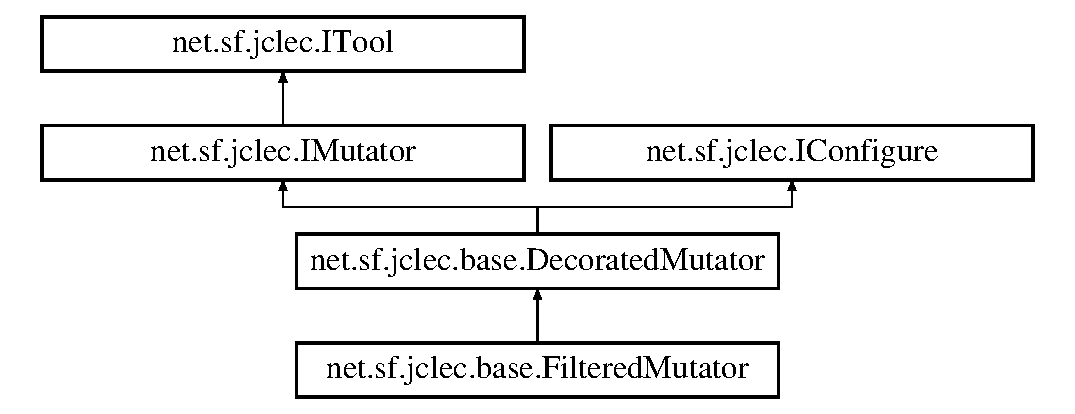
\includegraphics[height=4.000000cm]{classnet_1_1sf_1_1jclec_1_1base_1_1_filtered_mutator}
\end{center}
\end{figure}
\subsection*{Public Member Functions}
\begin{DoxyCompactItemize}
\item 
\hyperlink{classnet_1_1sf_1_1jclec_1_1base_1_1_filtered_mutator_a8d57508927040d3b1538ca3d2173a6ee}{Filtered\-Mutator} ()
\item 
\hyperlink{classnet_1_1sf_1_1jclec_1_1base_1_1_filtered_mutator_af32a7cbc7b7804064665f259462d21e5}{Filtered\-Mutator} (\hyperlink{interfacenet_1_1sf_1_1jclec_1_1_i_system}{I\-System} \hyperlink{classnet_1_1sf_1_1jclec_1_1base_1_1_decorated_mutator_a0f500ae1072a9663fa96475891c074bc}{context})
\item 
final double \hyperlink{classnet_1_1sf_1_1jclec_1_1base_1_1_filtered_mutator_ad7f2ca81314e6806dc6b2f4e18e3b25a}{get\-Mut\-Prob} ()
\item 
final void \hyperlink{classnet_1_1sf_1_1jclec_1_1base_1_1_filtered_mutator_a3d69423a21fea9eadf14aaa42c5784e3}{set\-Mut\-Prob} (double \hyperlink{classnet_1_1sf_1_1jclec_1_1base_1_1_filtered_mutator_ac5ca6f680430f923bc7e92a7de095721}{mut\-Prob})
\item 
void \hyperlink{classnet_1_1sf_1_1jclec_1_1base_1_1_filtered_mutator_ae5664f7971d88d670a061b2057774e83}{contextualize} (\hyperlink{interfacenet_1_1sf_1_1jclec_1_1_i_system}{I\-System} \hyperlink{classnet_1_1sf_1_1jclec_1_1base_1_1_decorated_mutator_a0f500ae1072a9663fa96475891c074bc}{context})
\item 
List$<$ \hyperlink{interfacenet_1_1sf_1_1jclec_1_1_i_individual}{I\-Individual} $>$ \hyperlink{classnet_1_1sf_1_1jclec_1_1base_1_1_filtered_mutator_a2664243ad8b112a7928ded718da6e5d5}{mutate} (List$<$ \hyperlink{interfacenet_1_1sf_1_1jclec_1_1_i_individual}{I\-Individual} $>$ parents)
\item 
List$<$ \hyperlink{interfacenet_1_1sf_1_1jclec_1_1_i_individual}{I\-Individual} $>$ \hyperlink{classnet_1_1sf_1_1jclec_1_1base_1_1_filtered_mutator_ac2b4533802c2048c60b176533e50c573}{get\-Sterile} ()
\item 
List$<$ \hyperlink{interfacenet_1_1sf_1_1jclec_1_1_i_individual}{I\-Individual} $>$ \hyperlink{classnet_1_1sf_1_1jclec_1_1base_1_1_filtered_mutator_ab7e133065fd51bde74cfc58d39c53e9a}{get\-Fertile} ()
\item 
void \hyperlink{classnet_1_1sf_1_1jclec_1_1base_1_1_filtered_mutator_a7927e4ea992f2c8dfff69ddd4d66b298}{configure} (Configuration settings)
\item 
boolean \hyperlink{classnet_1_1sf_1_1jclec_1_1base_1_1_filtered_mutator_ae142320a5476894c05893cbcdb25eaac}{equals} (Object other)
\end{DoxyCompactItemize}
\subsection*{Protected Attributes}
\begin{DoxyCompactItemize}
\item 
double \hyperlink{classnet_1_1sf_1_1jclec_1_1base_1_1_filtered_mutator_ac5ca6f680430f923bc7e92a7de095721}{mut\-Prob}
\item 
\hyperlink{interfacenet_1_1sf_1_1jclec_1_1util_1_1random_1_1_i_rand_gen}{I\-Rand\-Gen} \hyperlink{classnet_1_1sf_1_1jclec_1_1base_1_1_filtered_mutator_a846465d238479e38f6a752eed781cc2b}{randgen}
\item 
transient List$<$ \hyperlink{interfacenet_1_1sf_1_1jclec_1_1_i_individual}{I\-Individual} $>$ \hyperlink{classnet_1_1sf_1_1jclec_1_1base_1_1_filtered_mutator_aac6607c708d1937e2048a190da3d9b8b}{fertile} = new Array\-List$<$\hyperlink{interfacenet_1_1sf_1_1jclec_1_1_i_individual}{I\-Individual}$>$ ()
\item 
transient List$<$ \hyperlink{interfacenet_1_1sf_1_1jclec_1_1_i_individual}{I\-Individual} $>$ \hyperlink{classnet_1_1sf_1_1jclec_1_1base_1_1_filtered_mutator_a71f85310ce71199fa74922a7ed4d8088}{sterile} = new Array\-List$<$\hyperlink{interfacenet_1_1sf_1_1jclec_1_1_i_individual}{I\-Individual}$>$ ()
\end{DoxyCompactItemize}


\subsection{Detailed Description}
Filtered mutator. Mutates individuals with a given mutation probability.

\begin{DoxyAuthor}{Author}
Sebastian Ventura 
\end{DoxyAuthor}


\subsection{Constructor \& Destructor Documentation}
\hypertarget{classnet_1_1sf_1_1jclec_1_1base_1_1_filtered_mutator_a8d57508927040d3b1538ca3d2173a6ee}{\index{net\-::sf\-::jclec\-::base\-::\-Filtered\-Mutator@{net\-::sf\-::jclec\-::base\-::\-Filtered\-Mutator}!Filtered\-Mutator@{Filtered\-Mutator}}
\index{Filtered\-Mutator@{Filtered\-Mutator}!net::sf::jclec::base::FilteredMutator@{net\-::sf\-::jclec\-::base\-::\-Filtered\-Mutator}}
\subsubsection[{Filtered\-Mutator}]{\setlength{\rightskip}{0pt plus 5cm}net.\-sf.\-jclec.\-base.\-Filtered\-Mutator.\-Filtered\-Mutator (
\begin{DoxyParamCaption}
{}
\end{DoxyParamCaption}
)}}\label{classnet_1_1sf_1_1jclec_1_1base_1_1_filtered_mutator_a8d57508927040d3b1538ca3d2173a6ee}
Empty constructor \hypertarget{classnet_1_1sf_1_1jclec_1_1base_1_1_filtered_mutator_af32a7cbc7b7804064665f259462d21e5}{\index{net\-::sf\-::jclec\-::base\-::\-Filtered\-Mutator@{net\-::sf\-::jclec\-::base\-::\-Filtered\-Mutator}!Filtered\-Mutator@{Filtered\-Mutator}}
\index{Filtered\-Mutator@{Filtered\-Mutator}!net::sf::jclec::base::FilteredMutator@{net\-::sf\-::jclec\-::base\-::\-Filtered\-Mutator}}
\subsubsection[{Filtered\-Mutator}]{\setlength{\rightskip}{0pt plus 5cm}net.\-sf.\-jclec.\-base.\-Filtered\-Mutator.\-Filtered\-Mutator (
\begin{DoxyParamCaption}
\item[{{\bf I\-System}}]{context}
\end{DoxyParamCaption}
)}}\label{classnet_1_1sf_1_1jclec_1_1base_1_1_filtered_mutator_af32a7cbc7b7804064665f259462d21e5}
Constructor that contextualize this operator.


\begin{DoxyParams}{Parameters}
{\em context} & Execution context \\
\hline
\end{DoxyParams}


\subsection{Member Function Documentation}
\hypertarget{classnet_1_1sf_1_1jclec_1_1base_1_1_filtered_mutator_a7927e4ea992f2c8dfff69ddd4d66b298}{\index{net\-::sf\-::jclec\-::base\-::\-Filtered\-Mutator@{net\-::sf\-::jclec\-::base\-::\-Filtered\-Mutator}!configure@{configure}}
\index{configure@{configure}!net::sf::jclec::base::FilteredMutator@{net\-::sf\-::jclec\-::base\-::\-Filtered\-Mutator}}
\subsubsection[{configure}]{\setlength{\rightskip}{0pt plus 5cm}void net.\-sf.\-jclec.\-base.\-Filtered\-Mutator.\-configure (
\begin{DoxyParamCaption}
\item[{Configuration}]{settings}
\end{DoxyParamCaption}
)}}\label{classnet_1_1sf_1_1jclec_1_1base_1_1_filtered_mutator_a7927e4ea992f2c8dfff69ddd4d66b298}
Configuration method.


\begin{DoxyParams}{Parameters}
{\em settings} & Configuration settings \\
\hline
\end{DoxyParams}


Implements \hyperlink{interfacenet_1_1sf_1_1jclec_1_1_i_configure_add31a65a04d148c690a956fbbad6987c}{net.\-sf.\-jclec.\-I\-Configure}.

\hypertarget{classnet_1_1sf_1_1jclec_1_1base_1_1_filtered_mutator_ae5664f7971d88d670a061b2057774e83}{\index{net\-::sf\-::jclec\-::base\-::\-Filtered\-Mutator@{net\-::sf\-::jclec\-::base\-::\-Filtered\-Mutator}!contextualize@{contextualize}}
\index{contextualize@{contextualize}!net::sf::jclec::base::FilteredMutator@{net\-::sf\-::jclec\-::base\-::\-Filtered\-Mutator}}
\subsubsection[{contextualize}]{\setlength{\rightskip}{0pt plus 5cm}void net.\-sf.\-jclec.\-base.\-Filtered\-Mutator.\-contextualize (
\begin{DoxyParamCaption}
\item[{{\bf I\-System}}]{context}
\end{DoxyParamCaption}
)}}\label{classnet_1_1sf_1_1jclec_1_1base_1_1_filtered_mutator_ae5664f7971d88d670a061b2057774e83}
Contextualize decorated mutator (if exists)

Set the system where ...


\begin{DoxyParams}{Parameters}
{\em context} & Execution context\\
\hline
\end{DoxyParams}
 

Implements \hyperlink{interfacenet_1_1sf_1_1jclec_1_1_i_tool_aa11b3e046b7f38e40eb4f8c72a9a2102}{net.\-sf.\-jclec.\-I\-Tool}.

\hypertarget{classnet_1_1sf_1_1jclec_1_1base_1_1_filtered_mutator_ae142320a5476894c05893cbcdb25eaac}{\index{net\-::sf\-::jclec\-::base\-::\-Filtered\-Mutator@{net\-::sf\-::jclec\-::base\-::\-Filtered\-Mutator}!equals@{equals}}
\index{equals@{equals}!net::sf::jclec::base::FilteredMutator@{net\-::sf\-::jclec\-::base\-::\-Filtered\-Mutator}}
\subsubsection[{equals}]{\setlength{\rightskip}{0pt plus 5cm}boolean net.\-sf.\-jclec.\-base.\-Filtered\-Mutator.\-equals (
\begin{DoxyParamCaption}
\item[{Object}]{other}
\end{DoxyParamCaption}
)}}\label{classnet_1_1sf_1_1jclec_1_1base_1_1_filtered_mutator_ae142320a5476894c05893cbcdb25eaac}
Compare decorated mutator, mutation probability and randgen.\hypertarget{classnet_1_1sf_1_1jclec_1_1base_1_1_filtered_mutator_ab7e133065fd51bde74cfc58d39c53e9a}{\index{net\-::sf\-::jclec\-::base\-::\-Filtered\-Mutator@{net\-::sf\-::jclec\-::base\-::\-Filtered\-Mutator}!get\-Fertile@{get\-Fertile}}
\index{get\-Fertile@{get\-Fertile}!net::sf::jclec::base::FilteredMutator@{net\-::sf\-::jclec\-::base\-::\-Filtered\-Mutator}}
\subsubsection[{get\-Fertile}]{\setlength{\rightskip}{0pt plus 5cm}List$<${\bf I\-Individual}$>$ net.\-sf.\-jclec.\-base.\-Filtered\-Mutator.\-get\-Fertile (
\begin{DoxyParamCaption}
{}
\end{DoxyParamCaption}
)}}\label{classnet_1_1sf_1_1jclec_1_1base_1_1_filtered_mutator_ab7e133065fd51bde74cfc58d39c53e9a}
Access to the fertile parents set.

\begin{DoxyReturn}{Returns}
Fertile parents set 
\end{DoxyReturn}
\hypertarget{classnet_1_1sf_1_1jclec_1_1base_1_1_filtered_mutator_ad7f2ca81314e6806dc6b2f4e18e3b25a}{\index{net\-::sf\-::jclec\-::base\-::\-Filtered\-Mutator@{net\-::sf\-::jclec\-::base\-::\-Filtered\-Mutator}!get\-Mut\-Prob@{get\-Mut\-Prob}}
\index{get\-Mut\-Prob@{get\-Mut\-Prob}!net::sf::jclec::base::FilteredMutator@{net\-::sf\-::jclec\-::base\-::\-Filtered\-Mutator}}
\subsubsection[{get\-Mut\-Prob}]{\setlength{\rightskip}{0pt plus 5cm}final double net.\-sf.\-jclec.\-base.\-Filtered\-Mutator.\-get\-Mut\-Prob (
\begin{DoxyParamCaption}
{}
\end{DoxyParamCaption}
)}}\label{classnet_1_1sf_1_1jclec_1_1base_1_1_filtered_mutator_ad7f2ca81314e6806dc6b2f4e18e3b25a}
Access to \char`\"{}mut\-Prob\char`\"{} property.

\begin{DoxyReturn}{Returns}
Actual mutation probability 
\end{DoxyReturn}
\hypertarget{classnet_1_1sf_1_1jclec_1_1base_1_1_filtered_mutator_ac2b4533802c2048c60b176533e50c573}{\index{net\-::sf\-::jclec\-::base\-::\-Filtered\-Mutator@{net\-::sf\-::jclec\-::base\-::\-Filtered\-Mutator}!get\-Sterile@{get\-Sterile}}
\index{get\-Sterile@{get\-Sterile}!net::sf::jclec::base::FilteredMutator@{net\-::sf\-::jclec\-::base\-::\-Filtered\-Mutator}}
\subsubsection[{get\-Sterile}]{\setlength{\rightskip}{0pt plus 5cm}List$<${\bf I\-Individual}$>$ net.\-sf.\-jclec.\-base.\-Filtered\-Mutator.\-get\-Sterile (
\begin{DoxyParamCaption}
{}
\end{DoxyParamCaption}
)}}\label{classnet_1_1sf_1_1jclec_1_1base_1_1_filtered_mutator_ac2b4533802c2048c60b176533e50c573}
Access to the sterile parents set.

\begin{DoxyReturn}{Returns}
Sterile parents set 
\end{DoxyReturn}
\hypertarget{classnet_1_1sf_1_1jclec_1_1base_1_1_filtered_mutator_a2664243ad8b112a7928ded718da6e5d5}{\index{net\-::sf\-::jclec\-::base\-::\-Filtered\-Mutator@{net\-::sf\-::jclec\-::base\-::\-Filtered\-Mutator}!mutate@{mutate}}
\index{mutate@{mutate}!net::sf::jclec::base::FilteredMutator@{net\-::sf\-::jclec\-::base\-::\-Filtered\-Mutator}}
\subsubsection[{mutate}]{\setlength{\rightskip}{0pt plus 5cm}List$<${\bf I\-Individual}$>$ net.\-sf.\-jclec.\-base.\-Filtered\-Mutator.\-mutate (
\begin{DoxyParamCaption}
\item[{List$<$ {\bf I\-Individual} $>$}]{parents}
\end{DoxyParamCaption}
)}}\label{classnet_1_1sf_1_1jclec_1_1base_1_1_filtered_mutator_a2664243ad8b112a7928ded718da6e5d5}
This operator perform ... 

Implements \hyperlink{interfacenet_1_1sf_1_1jclec_1_1_i_mutator_a5300cd0df63950ea9f660b24425211fb}{net.\-sf.\-jclec.\-I\-Mutator}.

\hypertarget{classnet_1_1sf_1_1jclec_1_1base_1_1_filtered_mutator_a3d69423a21fea9eadf14aaa42c5784e3}{\index{net\-::sf\-::jclec\-::base\-::\-Filtered\-Mutator@{net\-::sf\-::jclec\-::base\-::\-Filtered\-Mutator}!set\-Mut\-Prob@{set\-Mut\-Prob}}
\index{set\-Mut\-Prob@{set\-Mut\-Prob}!net::sf::jclec::base::FilteredMutator@{net\-::sf\-::jclec\-::base\-::\-Filtered\-Mutator}}
\subsubsection[{set\-Mut\-Prob}]{\setlength{\rightskip}{0pt plus 5cm}final void net.\-sf.\-jclec.\-base.\-Filtered\-Mutator.\-set\-Mut\-Prob (
\begin{DoxyParamCaption}
\item[{double}]{mut\-Prob}
\end{DoxyParamCaption}
)}}\label{classnet_1_1sf_1_1jclec_1_1base_1_1_filtered_mutator_a3d69423a21fea9eadf14aaa42c5784e3}
Sets the \char`\"{}mut\-Prob\char`\"{} property.


\begin{DoxyParams}{Parameters}
{\em mut\-Prob} & New mutation probability \\
\hline
\end{DoxyParams}


\subsection{Member Data Documentation}
\hypertarget{classnet_1_1sf_1_1jclec_1_1base_1_1_filtered_mutator_aac6607c708d1937e2048a190da3d9b8b}{\index{net\-::sf\-::jclec\-::base\-::\-Filtered\-Mutator@{net\-::sf\-::jclec\-::base\-::\-Filtered\-Mutator}!fertile@{fertile}}
\index{fertile@{fertile}!net::sf::jclec::base::FilteredMutator@{net\-::sf\-::jclec\-::base\-::\-Filtered\-Mutator}}
\subsubsection[{fertile}]{\setlength{\rightskip}{0pt plus 5cm}transient List$<${\bf I\-Individual}$>$ net.\-sf.\-jclec.\-base.\-Filtered\-Mutator.\-fertile = new Array\-List$<${\bf I\-Individual}$>$ ()\hspace{0.3cm}{\ttfamily [protected]}}}\label{classnet_1_1sf_1_1jclec_1_1base_1_1_filtered_mutator_aac6607c708d1937e2048a190da3d9b8b}
Fertile parents set \hypertarget{classnet_1_1sf_1_1jclec_1_1base_1_1_filtered_mutator_ac5ca6f680430f923bc7e92a7de095721}{\index{net\-::sf\-::jclec\-::base\-::\-Filtered\-Mutator@{net\-::sf\-::jclec\-::base\-::\-Filtered\-Mutator}!mut\-Prob@{mut\-Prob}}
\index{mut\-Prob@{mut\-Prob}!net::sf::jclec::base::FilteredMutator@{net\-::sf\-::jclec\-::base\-::\-Filtered\-Mutator}}
\subsubsection[{mut\-Prob}]{\setlength{\rightskip}{0pt plus 5cm}double net.\-sf.\-jclec.\-base.\-Filtered\-Mutator.\-mut\-Prob\hspace{0.3cm}{\ttfamily [protected]}}}\label{classnet_1_1sf_1_1jclec_1_1base_1_1_filtered_mutator_ac5ca6f680430f923bc7e92a7de095721}
Mutation probability \hypertarget{classnet_1_1sf_1_1jclec_1_1base_1_1_filtered_mutator_a846465d238479e38f6a752eed781cc2b}{\index{net\-::sf\-::jclec\-::base\-::\-Filtered\-Mutator@{net\-::sf\-::jclec\-::base\-::\-Filtered\-Mutator}!randgen@{randgen}}
\index{randgen@{randgen}!net::sf::jclec::base::FilteredMutator@{net\-::sf\-::jclec\-::base\-::\-Filtered\-Mutator}}
\subsubsection[{randgen}]{\setlength{\rightskip}{0pt plus 5cm}{\bf I\-Rand\-Gen} net.\-sf.\-jclec.\-base.\-Filtered\-Mutator.\-randgen\hspace{0.3cm}{\ttfamily [protected]}}}\label{classnet_1_1sf_1_1jclec_1_1base_1_1_filtered_mutator_a846465d238479e38f6a752eed781cc2b}
Random generator \hypertarget{classnet_1_1sf_1_1jclec_1_1base_1_1_filtered_mutator_a71f85310ce71199fa74922a7ed4d8088}{\index{net\-::sf\-::jclec\-::base\-::\-Filtered\-Mutator@{net\-::sf\-::jclec\-::base\-::\-Filtered\-Mutator}!sterile@{sterile}}
\index{sterile@{sterile}!net::sf::jclec::base::FilteredMutator@{net\-::sf\-::jclec\-::base\-::\-Filtered\-Mutator}}
\subsubsection[{sterile}]{\setlength{\rightskip}{0pt plus 5cm}transient List$<${\bf I\-Individual}$>$ net.\-sf.\-jclec.\-base.\-Filtered\-Mutator.\-sterile = new Array\-List$<${\bf I\-Individual}$>$ ()\hspace{0.3cm}{\ttfamily [protected]}}}\label{classnet_1_1sf_1_1jclec_1_1base_1_1_filtered_mutator_a71f85310ce71199fa74922a7ed4d8088}
Sterile parents set 

The documentation for this class was generated from the following file\-:\begin{DoxyCompactItemize}
\item 
src/main/java/net/sf/jclec/base/Filtered\-Mutator.\-java\end{DoxyCompactItemize}

\hypertarget{classnet_1_1sf_1_1jclec_1_1base_1_1_filtered_recombinator}{\section{net.\-sf.\-jclec.\-base.\-Filtered\-Recombinator Class Reference}
\label{classnet_1_1sf_1_1jclec_1_1base_1_1_filtered_recombinator}\index{net.\-sf.\-jclec.\-base.\-Filtered\-Recombinator@{net.\-sf.\-jclec.\-base.\-Filtered\-Recombinator}}
}
Inheritance diagram for net.\-sf.\-jclec.\-base.\-Filtered\-Recombinator\-:\begin{figure}[H]
\begin{center}
\leavevmode
\includegraphics[height=4.000000cm]{classnet_1_1sf_1_1jclec_1_1base_1_1_filtered_recombinator}
\end{center}
\end{figure}
\subsection*{Public Member Functions}
\begin{DoxyCompactItemize}
\item 
\hyperlink{classnet_1_1sf_1_1jclec_1_1base_1_1_filtered_recombinator_a1a41eabc84e39fef2c99cc174a69e9b8}{Filtered\-Recombinator} ()
\item 
\hyperlink{classnet_1_1sf_1_1jclec_1_1base_1_1_filtered_recombinator_a2b4d7b17304238ffc20d71e0f4f1186f}{Filtered\-Recombinator} (\hyperlink{interfacenet_1_1sf_1_1jclec_1_1_i_system}{I\-System} \hyperlink{classnet_1_1sf_1_1jclec_1_1base_1_1_decorated_recombinator_a9fec99558ae7ddcf3ce82d8293305786}{context})
\item 
final double \hyperlink{classnet_1_1sf_1_1jclec_1_1base_1_1_filtered_recombinator_a887d9abe4e5e7fe134bbdc716387cb15}{get\-Rec\-Prob} ()
\item 
final void \hyperlink{classnet_1_1sf_1_1jclec_1_1base_1_1_filtered_recombinator_a21dbfdc8caf8740033e890061677ab76}{set\-Rec\-Prob} (double \hyperlink{classnet_1_1sf_1_1jclec_1_1base_1_1_filtered_recombinator_acadc9204c4432d1bb6ff5e8f4a085267}{rec\-Prob})
\item 
void \hyperlink{classnet_1_1sf_1_1jclec_1_1base_1_1_filtered_recombinator_ab492294f4c41c12c8832051623b225f4}{contextualize} (\hyperlink{interfacenet_1_1sf_1_1jclec_1_1_i_system}{I\-System} \hyperlink{classnet_1_1sf_1_1jclec_1_1base_1_1_decorated_recombinator_a9fec99558ae7ddcf3ce82d8293305786}{context})
\item 
List$<$ \hyperlink{interfacenet_1_1sf_1_1jclec_1_1_i_individual}{I\-Individual} $>$ \hyperlink{classnet_1_1sf_1_1jclec_1_1base_1_1_filtered_recombinator_a5611547b9db9f88087d817c2b896dcec}{recombine} (List$<$ \hyperlink{interfacenet_1_1sf_1_1jclec_1_1_i_individual}{I\-Individual} $>$ parents)
\item 
List$<$ \hyperlink{interfacenet_1_1sf_1_1jclec_1_1_i_individual}{I\-Individual} $>$ \hyperlink{classnet_1_1sf_1_1jclec_1_1base_1_1_filtered_recombinator_a757a0623d59a36acb068ada503edae20}{get\-Sterile} ()
\item 
List$<$ \hyperlink{interfacenet_1_1sf_1_1jclec_1_1_i_individual}{I\-Individual} $>$ \hyperlink{classnet_1_1sf_1_1jclec_1_1base_1_1_filtered_recombinator_a884f05ef201c32db04402b00e9069322}{get\-Fertile} ()
\item 
void \hyperlink{classnet_1_1sf_1_1jclec_1_1base_1_1_filtered_recombinator_abfcf757063e206f5c0ec482be5d9e9c1}{configure} (Configuration settings)
\item 
boolean \hyperlink{classnet_1_1sf_1_1jclec_1_1base_1_1_filtered_recombinator_ab14cc17cac864ee477e29e289601d30f}{equals} (Object other)
\end{DoxyCompactItemize}
\subsection*{Protected Attributes}
\begin{DoxyCompactItemize}
\item 
double \hyperlink{classnet_1_1sf_1_1jclec_1_1base_1_1_filtered_recombinator_acadc9204c4432d1bb6ff5e8f4a085267}{rec\-Prob}
\item 
\hyperlink{interfacenet_1_1sf_1_1jclec_1_1util_1_1random_1_1_i_rand_gen}{I\-Rand\-Gen} \hyperlink{classnet_1_1sf_1_1jclec_1_1base_1_1_filtered_recombinator_a8799959adcafbfb3928ed5b901925930}{randgen}
\item 
transient List$<$ \hyperlink{interfacenet_1_1sf_1_1jclec_1_1_i_individual}{I\-Individual} $>$ \hyperlink{classnet_1_1sf_1_1jclec_1_1base_1_1_filtered_recombinator_a11a8bd963d9617d71aa5b2cb834940b6}{fertile} = new Array\-List$<$\hyperlink{interfacenet_1_1sf_1_1jclec_1_1_i_individual}{I\-Individual}$>$ ()
\item 
transient List$<$ \hyperlink{interfacenet_1_1sf_1_1jclec_1_1_i_individual}{I\-Individual} $>$ \hyperlink{classnet_1_1sf_1_1jclec_1_1base_1_1_filtered_recombinator_a868d2538743c6926f579f1b7521011fa}{sterile} = new Array\-List$<$\hyperlink{interfacenet_1_1sf_1_1jclec_1_1_i_individual}{I\-Individual}$>$ ()
\end{DoxyCompactItemize}


\subsection{Detailed Description}
Filtered recombinator. Recombines individuals with a given recombination probability.

\begin{DoxyAuthor}{Author}
Sebastian Ventura 
\end{DoxyAuthor}


\subsection{Constructor \& Destructor Documentation}
\hypertarget{classnet_1_1sf_1_1jclec_1_1base_1_1_filtered_recombinator_a1a41eabc84e39fef2c99cc174a69e9b8}{\index{net\-::sf\-::jclec\-::base\-::\-Filtered\-Recombinator@{net\-::sf\-::jclec\-::base\-::\-Filtered\-Recombinator}!Filtered\-Recombinator@{Filtered\-Recombinator}}
\index{Filtered\-Recombinator@{Filtered\-Recombinator}!net::sf::jclec::base::FilteredRecombinator@{net\-::sf\-::jclec\-::base\-::\-Filtered\-Recombinator}}
\subsubsection[{Filtered\-Recombinator}]{\setlength{\rightskip}{0pt plus 5cm}net.\-sf.\-jclec.\-base.\-Filtered\-Recombinator.\-Filtered\-Recombinator (
\begin{DoxyParamCaption}
{}
\end{DoxyParamCaption}
)}}\label{classnet_1_1sf_1_1jclec_1_1base_1_1_filtered_recombinator_a1a41eabc84e39fef2c99cc174a69e9b8}
Empty constructor \hypertarget{classnet_1_1sf_1_1jclec_1_1base_1_1_filtered_recombinator_a2b4d7b17304238ffc20d71e0f4f1186f}{\index{net\-::sf\-::jclec\-::base\-::\-Filtered\-Recombinator@{net\-::sf\-::jclec\-::base\-::\-Filtered\-Recombinator}!Filtered\-Recombinator@{Filtered\-Recombinator}}
\index{Filtered\-Recombinator@{Filtered\-Recombinator}!net::sf::jclec::base::FilteredRecombinator@{net\-::sf\-::jclec\-::base\-::\-Filtered\-Recombinator}}
\subsubsection[{Filtered\-Recombinator}]{\setlength{\rightskip}{0pt plus 5cm}net.\-sf.\-jclec.\-base.\-Filtered\-Recombinator.\-Filtered\-Recombinator (
\begin{DoxyParamCaption}
\item[{{\bf I\-System}}]{context}
\end{DoxyParamCaption}
)}}\label{classnet_1_1sf_1_1jclec_1_1base_1_1_filtered_recombinator_a2b4d7b17304238ffc20d71e0f4f1186f}
Constructor that contextualize this operator.


\begin{DoxyParams}{Parameters}
{\em context} & Execution context \\
\hline
\end{DoxyParams}


\subsection{Member Function Documentation}
\hypertarget{classnet_1_1sf_1_1jclec_1_1base_1_1_filtered_recombinator_abfcf757063e206f5c0ec482be5d9e9c1}{\index{net\-::sf\-::jclec\-::base\-::\-Filtered\-Recombinator@{net\-::sf\-::jclec\-::base\-::\-Filtered\-Recombinator}!configure@{configure}}
\index{configure@{configure}!net::sf::jclec::base::FilteredRecombinator@{net\-::sf\-::jclec\-::base\-::\-Filtered\-Recombinator}}
\subsubsection[{configure}]{\setlength{\rightskip}{0pt plus 5cm}void net.\-sf.\-jclec.\-base.\-Filtered\-Recombinator.\-configure (
\begin{DoxyParamCaption}
\item[{Configuration}]{settings}
\end{DoxyParamCaption}
)}}\label{classnet_1_1sf_1_1jclec_1_1base_1_1_filtered_recombinator_abfcf757063e206f5c0ec482be5d9e9c1}
Configuration method.


\begin{DoxyParams}{Parameters}
{\em settings} & Configuration settings \\
\hline
\end{DoxyParams}


Implements \hyperlink{interfacenet_1_1sf_1_1jclec_1_1_i_configure_add31a65a04d148c690a956fbbad6987c}{net.\-sf.\-jclec.\-I\-Configure}.

\hypertarget{classnet_1_1sf_1_1jclec_1_1base_1_1_filtered_recombinator_ab492294f4c41c12c8832051623b225f4}{\index{net\-::sf\-::jclec\-::base\-::\-Filtered\-Recombinator@{net\-::sf\-::jclec\-::base\-::\-Filtered\-Recombinator}!contextualize@{contextualize}}
\index{contextualize@{contextualize}!net::sf::jclec::base::FilteredRecombinator@{net\-::sf\-::jclec\-::base\-::\-Filtered\-Recombinator}}
\subsubsection[{contextualize}]{\setlength{\rightskip}{0pt plus 5cm}void net.\-sf.\-jclec.\-base.\-Filtered\-Recombinator.\-contextualize (
\begin{DoxyParamCaption}
\item[{{\bf I\-System}}]{context}
\end{DoxyParamCaption}
)}}\label{classnet_1_1sf_1_1jclec_1_1base_1_1_filtered_recombinator_ab492294f4c41c12c8832051623b225f4}
Take a random generator and contextualize decorated recombinator (if exists)

Set the system where ...


\begin{DoxyParams}{Parameters}
{\em context} & Execution context\\
\hline
\end{DoxyParams}
 

Implements \hyperlink{interfacenet_1_1sf_1_1jclec_1_1_i_tool_aa11b3e046b7f38e40eb4f8c72a9a2102}{net.\-sf.\-jclec.\-I\-Tool}.

\hypertarget{classnet_1_1sf_1_1jclec_1_1base_1_1_filtered_recombinator_ab14cc17cac864ee477e29e289601d30f}{\index{net\-::sf\-::jclec\-::base\-::\-Filtered\-Recombinator@{net\-::sf\-::jclec\-::base\-::\-Filtered\-Recombinator}!equals@{equals}}
\index{equals@{equals}!net::sf::jclec::base::FilteredRecombinator@{net\-::sf\-::jclec\-::base\-::\-Filtered\-Recombinator}}
\subsubsection[{equals}]{\setlength{\rightskip}{0pt plus 5cm}boolean net.\-sf.\-jclec.\-base.\-Filtered\-Recombinator.\-equals (
\begin{DoxyParamCaption}
\item[{Object}]{other}
\end{DoxyParamCaption}
)}}\label{classnet_1_1sf_1_1jclec_1_1base_1_1_filtered_recombinator_ab14cc17cac864ee477e29e289601d30f}
Compare decorated mutator and mutation probability.\hypertarget{classnet_1_1sf_1_1jclec_1_1base_1_1_filtered_recombinator_a884f05ef201c32db04402b00e9069322}{\index{net\-::sf\-::jclec\-::base\-::\-Filtered\-Recombinator@{net\-::sf\-::jclec\-::base\-::\-Filtered\-Recombinator}!get\-Fertile@{get\-Fertile}}
\index{get\-Fertile@{get\-Fertile}!net::sf::jclec::base::FilteredRecombinator@{net\-::sf\-::jclec\-::base\-::\-Filtered\-Recombinator}}
\subsubsection[{get\-Fertile}]{\setlength{\rightskip}{0pt plus 5cm}List$<${\bf I\-Individual}$>$ net.\-sf.\-jclec.\-base.\-Filtered\-Recombinator.\-get\-Fertile (
\begin{DoxyParamCaption}
{}
\end{DoxyParamCaption}
)}}\label{classnet_1_1sf_1_1jclec_1_1base_1_1_filtered_recombinator_a884f05ef201c32db04402b00e9069322}
Access to the fertile parents set.

\begin{DoxyReturn}{Returns}
Fertile parents set 
\end{DoxyReturn}
\hypertarget{classnet_1_1sf_1_1jclec_1_1base_1_1_filtered_recombinator_a887d9abe4e5e7fe134bbdc716387cb15}{\index{net\-::sf\-::jclec\-::base\-::\-Filtered\-Recombinator@{net\-::sf\-::jclec\-::base\-::\-Filtered\-Recombinator}!get\-Rec\-Prob@{get\-Rec\-Prob}}
\index{get\-Rec\-Prob@{get\-Rec\-Prob}!net::sf::jclec::base::FilteredRecombinator@{net\-::sf\-::jclec\-::base\-::\-Filtered\-Recombinator}}
\subsubsection[{get\-Rec\-Prob}]{\setlength{\rightskip}{0pt plus 5cm}final double net.\-sf.\-jclec.\-base.\-Filtered\-Recombinator.\-get\-Rec\-Prob (
\begin{DoxyParamCaption}
{}
\end{DoxyParamCaption}
)}}\label{classnet_1_1sf_1_1jclec_1_1base_1_1_filtered_recombinator_a887d9abe4e5e7fe134bbdc716387cb15}
Access to \char`\"{}rec\-Prob\char`\"{} property.

\begin{DoxyReturn}{Returns}
Actual recombination probability 
\end{DoxyReturn}
\hypertarget{classnet_1_1sf_1_1jclec_1_1base_1_1_filtered_recombinator_a757a0623d59a36acb068ada503edae20}{\index{net\-::sf\-::jclec\-::base\-::\-Filtered\-Recombinator@{net\-::sf\-::jclec\-::base\-::\-Filtered\-Recombinator}!get\-Sterile@{get\-Sterile}}
\index{get\-Sterile@{get\-Sterile}!net::sf::jclec::base::FilteredRecombinator@{net\-::sf\-::jclec\-::base\-::\-Filtered\-Recombinator}}
\subsubsection[{get\-Sterile}]{\setlength{\rightskip}{0pt plus 5cm}List$<${\bf I\-Individual}$>$ net.\-sf.\-jclec.\-base.\-Filtered\-Recombinator.\-get\-Sterile (
\begin{DoxyParamCaption}
{}
\end{DoxyParamCaption}
)}}\label{classnet_1_1sf_1_1jclec_1_1base_1_1_filtered_recombinator_a757a0623d59a36acb068ada503edae20}
Access to the sterile parents set.

\begin{DoxyReturn}{Returns}
Sterile parents set 
\end{DoxyReturn}
\hypertarget{classnet_1_1sf_1_1jclec_1_1base_1_1_filtered_recombinator_a5611547b9db9f88087d817c2b896dcec}{\index{net\-::sf\-::jclec\-::base\-::\-Filtered\-Recombinator@{net\-::sf\-::jclec\-::base\-::\-Filtered\-Recombinator}!recombine@{recombine}}
\index{recombine@{recombine}!net::sf::jclec::base::FilteredRecombinator@{net\-::sf\-::jclec\-::base\-::\-Filtered\-Recombinator}}
\subsubsection[{recombine}]{\setlength{\rightskip}{0pt plus 5cm}List$<${\bf I\-Individual}$>$ net.\-sf.\-jclec.\-base.\-Filtered\-Recombinator.\-recombine (
\begin{DoxyParamCaption}
\item[{List$<$ {\bf I\-Individual} $>$}]{parents}
\end{DoxyParamCaption}
)}}\label{classnet_1_1sf_1_1jclec_1_1base_1_1_filtered_recombinator_a5611547b9db9f88087d817c2b896dcec}
This operator perform ...

Recombination method.


\begin{DoxyParams}{Parameters}
{\em parents} & Individuals to recombine\\
\hline
\end{DoxyParams}
\begin{DoxyReturn}{Returns}
Recombination result
\end{DoxyReturn}
 

Implements \hyperlink{interfacenet_1_1sf_1_1jclec_1_1_i_recombinator_a07721bb7be250aeae6a85e81c527e7a5}{net.\-sf.\-jclec.\-I\-Recombinator}.

\hypertarget{classnet_1_1sf_1_1jclec_1_1base_1_1_filtered_recombinator_a21dbfdc8caf8740033e890061677ab76}{\index{net\-::sf\-::jclec\-::base\-::\-Filtered\-Recombinator@{net\-::sf\-::jclec\-::base\-::\-Filtered\-Recombinator}!set\-Rec\-Prob@{set\-Rec\-Prob}}
\index{set\-Rec\-Prob@{set\-Rec\-Prob}!net::sf::jclec::base::FilteredRecombinator@{net\-::sf\-::jclec\-::base\-::\-Filtered\-Recombinator}}
\subsubsection[{set\-Rec\-Prob}]{\setlength{\rightskip}{0pt plus 5cm}final void net.\-sf.\-jclec.\-base.\-Filtered\-Recombinator.\-set\-Rec\-Prob (
\begin{DoxyParamCaption}
\item[{double}]{rec\-Prob}
\end{DoxyParamCaption}
)}}\label{classnet_1_1sf_1_1jclec_1_1base_1_1_filtered_recombinator_a21dbfdc8caf8740033e890061677ab76}
Sets the \char`\"{}rec\-Prob\char`\"{} property.


\begin{DoxyParams}{Parameters}
{\em rec\-Prob} & New recombination probability \\
\hline
\end{DoxyParams}


\subsection{Member Data Documentation}
\hypertarget{classnet_1_1sf_1_1jclec_1_1base_1_1_filtered_recombinator_a11a8bd963d9617d71aa5b2cb834940b6}{\index{net\-::sf\-::jclec\-::base\-::\-Filtered\-Recombinator@{net\-::sf\-::jclec\-::base\-::\-Filtered\-Recombinator}!fertile@{fertile}}
\index{fertile@{fertile}!net::sf::jclec::base::FilteredRecombinator@{net\-::sf\-::jclec\-::base\-::\-Filtered\-Recombinator}}
\subsubsection[{fertile}]{\setlength{\rightskip}{0pt plus 5cm}transient List$<${\bf I\-Individual}$>$ net.\-sf.\-jclec.\-base.\-Filtered\-Recombinator.\-fertile = new Array\-List$<${\bf I\-Individual}$>$ ()\hspace{0.3cm}{\ttfamily [protected]}}}\label{classnet_1_1sf_1_1jclec_1_1base_1_1_filtered_recombinator_a11a8bd963d9617d71aa5b2cb834940b6}
Fertile parents set \hypertarget{classnet_1_1sf_1_1jclec_1_1base_1_1_filtered_recombinator_a8799959adcafbfb3928ed5b901925930}{\index{net\-::sf\-::jclec\-::base\-::\-Filtered\-Recombinator@{net\-::sf\-::jclec\-::base\-::\-Filtered\-Recombinator}!randgen@{randgen}}
\index{randgen@{randgen}!net::sf::jclec::base::FilteredRecombinator@{net\-::sf\-::jclec\-::base\-::\-Filtered\-Recombinator}}
\subsubsection[{randgen}]{\setlength{\rightskip}{0pt plus 5cm}{\bf I\-Rand\-Gen} net.\-sf.\-jclec.\-base.\-Filtered\-Recombinator.\-randgen\hspace{0.3cm}{\ttfamily [protected]}}}\label{classnet_1_1sf_1_1jclec_1_1base_1_1_filtered_recombinator_a8799959adcafbfb3928ed5b901925930}
Random generator \hypertarget{classnet_1_1sf_1_1jclec_1_1base_1_1_filtered_recombinator_acadc9204c4432d1bb6ff5e8f4a085267}{\index{net\-::sf\-::jclec\-::base\-::\-Filtered\-Recombinator@{net\-::sf\-::jclec\-::base\-::\-Filtered\-Recombinator}!rec\-Prob@{rec\-Prob}}
\index{rec\-Prob@{rec\-Prob}!net::sf::jclec::base::FilteredRecombinator@{net\-::sf\-::jclec\-::base\-::\-Filtered\-Recombinator}}
\subsubsection[{rec\-Prob}]{\setlength{\rightskip}{0pt plus 5cm}double net.\-sf.\-jclec.\-base.\-Filtered\-Recombinator.\-rec\-Prob\hspace{0.3cm}{\ttfamily [protected]}}}\label{classnet_1_1sf_1_1jclec_1_1base_1_1_filtered_recombinator_acadc9204c4432d1bb6ff5e8f4a085267}
Mutation probability \hypertarget{classnet_1_1sf_1_1jclec_1_1base_1_1_filtered_recombinator_a868d2538743c6926f579f1b7521011fa}{\index{net\-::sf\-::jclec\-::base\-::\-Filtered\-Recombinator@{net\-::sf\-::jclec\-::base\-::\-Filtered\-Recombinator}!sterile@{sterile}}
\index{sterile@{sterile}!net::sf::jclec::base::FilteredRecombinator@{net\-::sf\-::jclec\-::base\-::\-Filtered\-Recombinator}}
\subsubsection[{sterile}]{\setlength{\rightskip}{0pt plus 5cm}transient List$<${\bf I\-Individual}$>$ net.\-sf.\-jclec.\-base.\-Filtered\-Recombinator.\-sterile = new Array\-List$<${\bf I\-Individual}$>$ ()\hspace{0.3cm}{\ttfamily [protected]}}}\label{classnet_1_1sf_1_1jclec_1_1base_1_1_filtered_recombinator_a868d2538743c6926f579f1b7521011fa}
Sterile parents set 

The documentation for this class was generated from the following file\-:\begin{DoxyCompactItemize}
\item 
src/main/java/net/sf/jclec/base/Filtered\-Recombinator.\-java\end{DoxyCompactItemize}

\hypertarget{classnet_1_1sf_1_1jclec_1_1base_1_1_filtered_recombinator_test}{\section{net.\-sf.\-jclec.\-base.\-Filtered\-Recombinator\-Test Class Reference}
\label{classnet_1_1sf_1_1jclec_1_1base_1_1_filtered_recombinator_test}\index{net.\-sf.\-jclec.\-base.\-Filtered\-Recombinator\-Test@{net.\-sf.\-jclec.\-base.\-Filtered\-Recombinator\-Test}}
}


Inherits I\-Tool\-Test$<$ Filtered\-Recombinator $>$.

\subsection*{Public Member Functions}
\begin{DoxyCompactItemize}
\item 
void \hyperlink{classnet_1_1sf_1_1jclec_1_1base_1_1_filtered_recombinator_test_aed51c3837575bfeeba8ca15e9810fb31}{test\-Recombine} ()
\end{DoxyCompactItemize}


\subsection{Detailed Description}
\hyperlink{classnet_1_1sf_1_1jclec_1_1base_1_1_filtered_recombinator}{Filtered\-Recombinator} test.

\begin{DoxyAuthor}{Author}
Sebastian Ventura Soto 
\end{DoxyAuthor}


\subsection{Member Function Documentation}
\hypertarget{classnet_1_1sf_1_1jclec_1_1base_1_1_filtered_recombinator_test_aed51c3837575bfeeba8ca15e9810fb31}{\index{net\-::sf\-::jclec\-::base\-::\-Filtered\-Recombinator\-Test@{net\-::sf\-::jclec\-::base\-::\-Filtered\-Recombinator\-Test}!test\-Recombine@{test\-Recombine}}
\index{test\-Recombine@{test\-Recombine}!net::sf::jclec::base::FilteredRecombinatorTest@{net\-::sf\-::jclec\-::base\-::\-Filtered\-Recombinator\-Test}}
\subsubsection[{test\-Recombine}]{\setlength{\rightskip}{0pt plus 5cm}void net.\-sf.\-jclec.\-base.\-Filtered\-Recombinator\-Test.\-test\-Recombine (
\begin{DoxyParamCaption}
{}
\end{DoxyParamCaption}
)}}\label{classnet_1_1sf_1_1jclec_1_1base_1_1_filtered_recombinator_test_aed51c3837575bfeeba8ca15e9810fb31}
Unit test for recombine() test 

The documentation for this class was generated from the following file\-:\begin{DoxyCompactItemize}
\item 
src/test/java/net/sf/jclec/base/Filtered\-Recombinator\-Test.\-java\end{DoxyCompactItemize}

\hypertarget{classnet_1_1sf_1_1jclec_1_1realarray_1_1rec_1_1_flat_crossover}{\section{net.\-sf.\-jclec.\-realarray.\-rec.\-Flat\-Crossover Class Reference}
\label{classnet_1_1sf_1_1jclec_1_1realarray_1_1rec_1_1_flat_crossover}\index{net.\-sf.\-jclec.\-realarray.\-rec.\-Flat\-Crossover@{net.\-sf.\-jclec.\-realarray.\-rec.\-Flat\-Crossover}}
}


Inherits net.\-sf.\-jclec.\-realarray.\-rec.\-Uniform\-Crossover2x1.

\subsection*{Public Member Functions}
\begin{DoxyCompactItemize}
\item 
\hyperlink{classnet_1_1sf_1_1jclec_1_1realarray_1_1rec_1_1_flat_crossover_a7b870a24cbcdc0dad5a66e809ac57d94}{Flat\-Crossover} ()
\end{DoxyCompactItemize}
\subsection*{Protected Member Functions}
\begin{DoxyCompactItemize}
\item 
double \hyperlink{classnet_1_1sf_1_1jclec_1_1realarray_1_1rec_1_1_flat_crossover_a1c517b81d958cba11ea7cee6167c2616}{default\-Locus\-Rec\-Prob} ()
\end{DoxyCompactItemize}
\subsection*{Additional Inherited Members}


\subsection{Detailed Description}
Apply a flat crossover for two individuals.

\begin{DoxyAuthor}{Author}
Alberto Lamarca 

Sebastian Ventura 
\end{DoxyAuthor}


\subsection{Constructor \& Destructor Documentation}
\hypertarget{classnet_1_1sf_1_1jclec_1_1realarray_1_1rec_1_1_flat_crossover_a7b870a24cbcdc0dad5a66e809ac57d94}{\index{net\-::sf\-::jclec\-::realarray\-::rec\-::\-Flat\-Crossover@{net\-::sf\-::jclec\-::realarray\-::rec\-::\-Flat\-Crossover}!Flat\-Crossover@{Flat\-Crossover}}
\index{Flat\-Crossover@{Flat\-Crossover}!net::sf::jclec::realarray::rec::FlatCrossover@{net\-::sf\-::jclec\-::realarray\-::rec\-::\-Flat\-Crossover}}
\subsubsection[{Flat\-Crossover}]{\setlength{\rightskip}{0pt plus 5cm}net.\-sf.\-jclec.\-realarray.\-rec.\-Flat\-Crossover.\-Flat\-Crossover (
\begin{DoxyParamCaption}
{}
\end{DoxyParamCaption}
)}}\label{classnet_1_1sf_1_1jclec_1_1realarray_1_1rec_1_1_flat_crossover_a7b870a24cbcdc0dad5a66e809ac57d94}
Empty constructor 

\subsection{Member Function Documentation}
\hypertarget{classnet_1_1sf_1_1jclec_1_1realarray_1_1rec_1_1_flat_crossover_a1c517b81d958cba11ea7cee6167c2616}{\index{net\-::sf\-::jclec\-::realarray\-::rec\-::\-Flat\-Crossover@{net\-::sf\-::jclec\-::realarray\-::rec\-::\-Flat\-Crossover}!default\-Locus\-Rec\-Prob@{default\-Locus\-Rec\-Prob}}
\index{default\-Locus\-Rec\-Prob@{default\-Locus\-Rec\-Prob}!net::sf::jclec::realarray::rec::FlatCrossover@{net\-::sf\-::jclec\-::realarray\-::rec\-::\-Flat\-Crossover}}
\subsubsection[{default\-Locus\-Rec\-Prob}]{\setlength{\rightskip}{0pt plus 5cm}double net.\-sf.\-jclec.\-realarray.\-rec.\-Flat\-Crossover.\-default\-Locus\-Rec\-Prob (
\begin{DoxyParamCaption}
{}
\end{DoxyParamCaption}
)\hspace{0.3cm}{\ttfamily [protected]}, {\ttfamily [virtual]}}}\label{classnet_1_1sf_1_1jclec_1_1realarray_1_1rec_1_1_flat_crossover_a1c517b81d958cba11ea7cee6167c2616}
Get default value for this parameter. 

Implements \hyperlink{classnet_1_1sf_1_1jclec_1_1realarray_1_1_uniform_crossover_ac427b4ae11cf8b9495625005fe5ec575}{net.\-sf.\-jclec.\-realarray.\-Uniform\-Crossover}.



The documentation for this class was generated from the following file\-:\begin{DoxyCompactItemize}
\item 
src/main/java/net/sf/jclec/realarray/rec/Flat\-Crossover.\-java\end{DoxyCompactItemize}

\hypertarget{classnet_1_1sf_1_1jclec_1_1algorithm_1_1gengap_1_1_g3}{\section{net.\-sf.\-jclec.\-algorithm.\-gengap.\-G3 Class Reference}
\label{classnet_1_1sf_1_1jclec_1_1algorithm_1_1gengap_1_1_g3}\index{net.\-sf.\-jclec.\-algorithm.\-gengap.\-G3@{net.\-sf.\-jclec.\-algorithm.\-gengap.\-G3}}
}
Inheritance diagram for net.\-sf.\-jclec.\-algorithm.\-gengap.\-G3\-:\begin{figure}[H]
\begin{center}
\leavevmode
\includegraphics[height=5.000000cm]{classnet_1_1sf_1_1jclec_1_1algorithm_1_1gengap_1_1_g3}
\end{center}
\end{figure}
\subsection*{Public Member Functions}
\begin{DoxyCompactItemize}
\item 
\hyperlink{classnet_1_1sf_1_1jclec_1_1algorithm_1_1gengap_1_1_g3_a51512b95f02cf096d4e3ad1707cea740}{G3} ()
\item 
\hyperlink{interfacenet_1_1sf_1_1jclec_1_1_i_recombinator}{I\-Recombinator} \hyperlink{classnet_1_1sf_1_1jclec_1_1algorithm_1_1gengap_1_1_g3_a01270bb20828c11e75b92f19bde0c410}{get\-Recombinator} ()
\item 
void \hyperlink{classnet_1_1sf_1_1jclec_1_1algorithm_1_1gengap_1_1_g3_a32a85d47f3a78b60b571abe6abadb804}{set\-Recombinator} (\hyperlink{interfacenet_1_1sf_1_1jclec_1_1_i_recombinator}{I\-Recombinator} \hyperlink{classnet_1_1sf_1_1jclec_1_1algorithm_1_1gengap_1_1_g3_a079407128e3e5eb01b3777e5e7a9c488}{recombinator})
\item 
final int \hyperlink{classnet_1_1sf_1_1jclec_1_1algorithm_1_1gengap_1_1_g3_a49904604450e461b226314bc3219054a}{get\-Mu} ()
\item 
final void \hyperlink{classnet_1_1sf_1_1jclec_1_1algorithm_1_1gengap_1_1_g3_a2ad0b2486a6700e36d0be0c2ab07c1dc}{set\-Mu} (int \hyperlink{classnet_1_1sf_1_1jclec_1_1algorithm_1_1gengap_1_1_g3_aa4ddf4a074688412a3fe669aac3283a1}{mu})
\item 
final int \hyperlink{classnet_1_1sf_1_1jclec_1_1algorithm_1_1gengap_1_1_g3_a5ea993b026f651ac96864ed504096f89}{get\-Lambda} ()
\item 
final void \hyperlink{classnet_1_1sf_1_1jclec_1_1algorithm_1_1gengap_1_1_g3_af019015e3f69f52f6944ed498b7a5df3}{set\-Lambda} (int \hyperlink{classnet_1_1sf_1_1jclec_1_1algorithm_1_1gengap_1_1_g3_ad0bae64a81015d9bfd89a37a1273ae05}{lambda})
\item 
final int \hyperlink{classnet_1_1sf_1_1jclec_1_1algorithm_1_1gengap_1_1_g3_af092f90203be10fd462c385e78d44bbb}{get\-R} ()
\item 
final void \hyperlink{classnet_1_1sf_1_1jclec_1_1algorithm_1_1gengap_1_1_g3_a2b92c40476ac5188c83e42528caf00d6}{set\-R} (int \hyperlink{classnet_1_1sf_1_1jclec_1_1algorithm_1_1gengap_1_1_g3_ab4b67f3578c57a6c888a620f90d02c0e}{r})
\item 
void \hyperlink{classnet_1_1sf_1_1jclec_1_1algorithm_1_1gengap_1_1_g3_a4453ecc8819a46cc733d5f3792b19e78}{configure} (Configuration configuration)
\item 
void \hyperlink{classnet_1_1sf_1_1jclec_1_1algorithm_1_1gengap_1_1_g3_aa63856d552765e073a18a74708555e18}{do\-Init} ()
\end{DoxyCompactItemize}
\subsection*{Protected Member Functions}
\begin{DoxyCompactItemize}
\item 
void \hyperlink{classnet_1_1sf_1_1jclec_1_1algorithm_1_1gengap_1_1_g3_ad03cfbc667a5d79751ca91410e1f4b35}{do\-Selection} ()
\item 
void \hyperlink{classnet_1_1sf_1_1jclec_1_1algorithm_1_1gengap_1_1_g3_a423dbceb7b8ba0580aee18d982fbd428}{do\-Generation} ()
\item 
void \hyperlink{classnet_1_1sf_1_1jclec_1_1algorithm_1_1gengap_1_1_g3_afd9e833c748f22790598dba7ec39cedb}{do\-Replacement} ()
\item 
void \hyperlink{classnet_1_1sf_1_1jclec_1_1algorithm_1_1gengap_1_1_g3_ade2342ab60873a250aab76eb522b5948}{do\-Update} ()
\end{DoxyCompactItemize}
\subsection*{Protected Attributes}
\begin{DoxyCompactItemize}
\item 
int \hyperlink{classnet_1_1sf_1_1jclec_1_1algorithm_1_1gengap_1_1_g3_aa4ddf4a074688412a3fe669aac3283a1}{mu}
\item 
int \hyperlink{classnet_1_1sf_1_1jclec_1_1algorithm_1_1gengap_1_1_g3_ad0bae64a81015d9bfd89a37a1273ae05}{lambda}
\item 
\hyperlink{classnet_1_1sf_1_1jclec_1_1base_1_1_repeat_recombinator}{Repeat\-Recombinator} \hyperlink{classnet_1_1sf_1_1jclec_1_1algorithm_1_1gengap_1_1_g3_a079407128e3e5eb01b3777e5e7a9c488}{recombinator}
\item 
int \hyperlink{classnet_1_1sf_1_1jclec_1_1algorithm_1_1gengap_1_1_g3_ab4b67f3578c57a6c888a620f90d02c0e}{r}
\item 
transient \hyperlink{classnet_1_1sf_1_1jclec_1_1selector_1_1_random_selector}{Random\-Selector} \hyperlink{classnet_1_1sf_1_1jclec_1_1algorithm_1_1gengap_1_1_g3_a57dd3e0c92be45cb3ab1601a2b216da5}{parents\-Selector}
\item 
transient \hyperlink{classnet_1_1sf_1_1jclec_1_1selector_1_1_random_selector}{Random\-Selector} \hyperlink{classnet_1_1sf_1_1jclec_1_1algorithm_1_1gengap_1_1_g3_ae51e516d5ceb1f80ae931bce9319d255}{replacement\-Selector}
\item 
transient \hyperlink{classnet_1_1sf_1_1jclec_1_1selector_1_1_roulette_selector}{Roulette\-Selector} \hyperlink{classnet_1_1sf_1_1jclec_1_1algorithm_1_1gengap_1_1_g3_ac9eb67ba0b3d5f8a0301e9df03ec5130}{update\-Selector}
\item 
transient \hyperlink{classnet_1_1sf_1_1jclec_1_1selector_1_1_betters_selector}{Betters\-Selector} \hyperlink{classnet_1_1sf_1_1jclec_1_1algorithm_1_1gengap_1_1_g3_aeec51201a8db026697691e93b2c8b026}{betters\-Selector}
\end{DoxyCompactItemize}


\subsection{Detailed Description}
{\bfseries $<$u$>$G$<$/u$>$}eneralized {\bfseries $<$u$>$G$<$/u$>$}eneration {\bfseries $<$u$>$G$<$/u$>$}ap algorithm.

\begin{DoxyAuthor}{Author}
Maria Catala-\/\-Carbonero 

Sebastian Ventura 

Carlos Garcia-\/\-Martinez 
\end{DoxyAuthor}


\subsection{Constructor \& Destructor Documentation}
\hypertarget{classnet_1_1sf_1_1jclec_1_1algorithm_1_1gengap_1_1_g3_a51512b95f02cf096d4e3ad1707cea740}{\index{net\-::sf\-::jclec\-::algorithm\-::gengap\-::\-G3@{net\-::sf\-::jclec\-::algorithm\-::gengap\-::\-G3}!G3@{G3}}
\index{G3@{G3}!net::sf::jclec::algorithm::gengap::G3@{net\-::sf\-::jclec\-::algorithm\-::gengap\-::\-G3}}
\subsubsection[{G3}]{\setlength{\rightskip}{0pt plus 5cm}net.\-sf.\-jclec.\-algorithm.\-gengap.\-G3.\-G3 (
\begin{DoxyParamCaption}
{}
\end{DoxyParamCaption}
)}}\label{classnet_1_1sf_1_1jclec_1_1algorithm_1_1gengap_1_1_g3_a51512b95f02cf096d4e3ad1707cea740}
Empty (default) constructor 

\subsection{Member Function Documentation}
\hypertarget{classnet_1_1sf_1_1jclec_1_1algorithm_1_1gengap_1_1_g3_a4453ecc8819a46cc733d5f3792b19e78}{\index{net\-::sf\-::jclec\-::algorithm\-::gengap\-::\-G3@{net\-::sf\-::jclec\-::algorithm\-::gengap\-::\-G3}!configure@{configure}}
\index{configure@{configure}!net::sf::jclec::algorithm::gengap::G3@{net\-::sf\-::jclec\-::algorithm\-::gengap\-::\-G3}}
\subsubsection[{configure}]{\setlength{\rightskip}{0pt plus 5cm}void net.\-sf.\-jclec.\-algorithm.\-gengap.\-G3.\-configure (
\begin{DoxyParamCaption}
\item[{Configuration}]{configuration}
\end{DoxyParamCaption}
)}}\label{classnet_1_1sf_1_1jclec_1_1algorithm_1_1gengap_1_1_g3_a4453ecc8819a46cc733d5f3792b19e78}
Configuration method.

Configuration parameters for Base\-Algorithm class are\-:


\begin{DoxyItemize}
\item {\ttfamily species\-: \hyperlink{interfacenet_1_1sf_1_1jclec_1_1_i_species}{I\-Species} (complex)}

Individual species 
\item {\ttfamily evaluator\-: \hyperlink{interfacenet_1_1sf_1_1jclec_1_1_i_evaluator}{I\-Evaluator} (complex)}

Individuals evaluator 
\item {\ttfamily population-\/size\-: int}

\hyperlink{classnet_1_1sf_1_1jclec_1_1_population}{Population} size 
\item {\ttfamily max-\/of-\/generations\-: int}

Maximum number of generations  
\item {\ttfamily provider\-: \hyperlink{interfacenet_1_1sf_1_1jclec_1_1_i_provider}{I\-Provider} (complex)}

Individuals provider  
\item {\ttfamily mu\-: int} Number of parents to select  
\item {\ttfamily lambda\-: int} Number of son to obtain by recombination  
\item {\ttfamily recombinator\-: \hyperlink{interfacenet_1_1sf_1_1jclec_1_1_i_recombinator}{I\-Recombinator} (complex)} Recombination operator  
\end{DoxyItemize}

Implements \hyperlink{interfacenet_1_1sf_1_1jclec_1_1_i_configure_add31a65a04d148c690a956fbbad6987c}{net.\-sf.\-jclec.\-I\-Configure}.

\hypertarget{classnet_1_1sf_1_1jclec_1_1algorithm_1_1gengap_1_1_g3_a423dbceb7b8ba0580aee18d982fbd428}{\index{net\-::sf\-::jclec\-::algorithm\-::gengap\-::\-G3@{net\-::sf\-::jclec\-::algorithm\-::gengap\-::\-G3}!do\-Generation@{do\-Generation}}
\index{do\-Generation@{do\-Generation}!net::sf::jclec::algorithm::gengap::G3@{net\-::sf\-::jclec\-::algorithm\-::gengap\-::\-G3}}
\subsubsection[{do\-Generation}]{\setlength{\rightskip}{0pt plus 5cm}void net.\-sf.\-jclec.\-algorithm.\-gengap.\-G3.\-do\-Generation (
\begin{DoxyParamCaption}
{}
\end{DoxyParamCaption}
)\hspace{0.3cm}{\ttfamily [protected]}, {\ttfamily [virtual]}}}\label{classnet_1_1sf_1_1jclec_1_1algorithm_1_1gengap_1_1_g3_a423dbceb7b8ba0580aee18d982fbd428}
Generate new individuals from parents 

Implements \hyperlink{classnet_1_1sf_1_1jclec_1_1algorithm_1_1_population_algorithm_a04894ec2d7f9e72eca1a41127bd1c7d3}{net.\-sf.\-jclec.\-algorithm.\-Population\-Algorithm}.

\hypertarget{classnet_1_1sf_1_1jclec_1_1algorithm_1_1gengap_1_1_g3_aa63856d552765e073a18a74708555e18}{\index{net\-::sf\-::jclec\-::algorithm\-::gengap\-::\-G3@{net\-::sf\-::jclec\-::algorithm\-::gengap\-::\-G3}!do\-Init@{do\-Init}}
\index{do\-Init@{do\-Init}!net::sf::jclec::algorithm::gengap::G3@{net\-::sf\-::jclec\-::algorithm\-::gengap\-::\-G3}}
\subsubsection[{do\-Init}]{\setlength{\rightskip}{0pt plus 5cm}void net.\-sf.\-jclec.\-algorithm.\-gengap.\-G3.\-do\-Init (
\begin{DoxyParamCaption}
{}
\end{DoxyParamCaption}
)\hspace{0.3cm}{\ttfamily [virtual]}}}\label{classnet_1_1sf_1_1jclec_1_1algorithm_1_1gengap_1_1_g3_aa63856d552765e073a18a74708555e18}
Perform algorithm initialization. 

Implements \hyperlink{classnet_1_1sf_1_1jclec_1_1algorithm_1_1_abstract_algorithm_a9cb5c0abb0c171944290260eccbc0078}{net.\-sf.\-jclec.\-algorithm.\-Abstract\-Algorithm}.

\hypertarget{classnet_1_1sf_1_1jclec_1_1algorithm_1_1gengap_1_1_g3_afd9e833c748f22790598dba7ec39cedb}{\index{net\-::sf\-::jclec\-::algorithm\-::gengap\-::\-G3@{net\-::sf\-::jclec\-::algorithm\-::gengap\-::\-G3}!do\-Replacement@{do\-Replacement}}
\index{do\-Replacement@{do\-Replacement}!net::sf::jclec::algorithm::gengap::G3@{net\-::sf\-::jclec\-::algorithm\-::gengap\-::\-G3}}
\subsubsection[{do\-Replacement}]{\setlength{\rightskip}{0pt plus 5cm}void net.\-sf.\-jclec.\-algorithm.\-gengap.\-G3.\-do\-Replacement (
\begin{DoxyParamCaption}
{}
\end{DoxyParamCaption}
)\hspace{0.3cm}{\ttfamily [protected]}, {\ttfamily [virtual]}}}\label{classnet_1_1sf_1_1jclec_1_1algorithm_1_1gengap_1_1_g3_afd9e833c748f22790598dba7ec39cedb}
Select individuals to extinct in this generation. 

Implements \hyperlink{classnet_1_1sf_1_1jclec_1_1algorithm_1_1_population_algorithm_afac7f83430707d572fbe8a2ea79c3685}{net.\-sf.\-jclec.\-algorithm.\-Population\-Algorithm}.

\hypertarget{classnet_1_1sf_1_1jclec_1_1algorithm_1_1gengap_1_1_g3_ad03cfbc667a5d79751ca91410e1f4b35}{\index{net\-::sf\-::jclec\-::algorithm\-::gengap\-::\-G3@{net\-::sf\-::jclec\-::algorithm\-::gengap\-::\-G3}!do\-Selection@{do\-Selection}}
\index{do\-Selection@{do\-Selection}!net::sf::jclec::algorithm::gengap::G3@{net\-::sf\-::jclec\-::algorithm\-::gengap\-::\-G3}}
\subsubsection[{do\-Selection}]{\setlength{\rightskip}{0pt plus 5cm}void net.\-sf.\-jclec.\-algorithm.\-gengap.\-G3.\-do\-Selection (
\begin{DoxyParamCaption}
{}
\end{DoxyParamCaption}
)\hspace{0.3cm}{\ttfamily [protected]}, {\ttfamily [virtual]}}}\label{classnet_1_1sf_1_1jclec_1_1algorithm_1_1gengap_1_1_g3_ad03cfbc667a5d79751ca91410e1f4b35}
Select individuals to be breeded. 

Implements \hyperlink{classnet_1_1sf_1_1jclec_1_1algorithm_1_1_population_algorithm_a0c3b482671dc8c454f968a30a374c3be}{net.\-sf.\-jclec.\-algorithm.\-Population\-Algorithm}.

\hypertarget{classnet_1_1sf_1_1jclec_1_1algorithm_1_1gengap_1_1_g3_ade2342ab60873a250aab76eb522b5948}{\index{net\-::sf\-::jclec\-::algorithm\-::gengap\-::\-G3@{net\-::sf\-::jclec\-::algorithm\-::gengap\-::\-G3}!do\-Update@{do\-Update}}
\index{do\-Update@{do\-Update}!net::sf::jclec::algorithm::gengap::G3@{net\-::sf\-::jclec\-::algorithm\-::gengap\-::\-G3}}
\subsubsection[{do\-Update}]{\setlength{\rightskip}{0pt plus 5cm}void net.\-sf.\-jclec.\-algorithm.\-gengap.\-G3.\-do\-Update (
\begin{DoxyParamCaption}
{}
\end{DoxyParamCaption}
)\hspace{0.3cm}{\ttfamily [protected]}, {\ttfamily [virtual]}}}\label{classnet_1_1sf_1_1jclec_1_1algorithm_1_1gengap_1_1_g3_ade2342ab60873a250aab76eb522b5948}
Update population individuals. 

Implements \hyperlink{classnet_1_1sf_1_1jclec_1_1algorithm_1_1_population_algorithm_a0817186f210c38255cc46f490cbbf53e}{net.\-sf.\-jclec.\-algorithm.\-Population\-Algorithm}.

\hypertarget{classnet_1_1sf_1_1jclec_1_1algorithm_1_1gengap_1_1_g3_a5ea993b026f651ac96864ed504096f89}{\index{net\-::sf\-::jclec\-::algorithm\-::gengap\-::\-G3@{net\-::sf\-::jclec\-::algorithm\-::gengap\-::\-G3}!get\-Lambda@{get\-Lambda}}
\index{get\-Lambda@{get\-Lambda}!net::sf::jclec::algorithm::gengap::G3@{net\-::sf\-::jclec\-::algorithm\-::gengap\-::\-G3}}
\subsubsection[{get\-Lambda}]{\setlength{\rightskip}{0pt plus 5cm}final int net.\-sf.\-jclec.\-algorithm.\-gengap.\-G3.\-get\-Lambda (
\begin{DoxyParamCaption}
{}
\end{DoxyParamCaption}
)}}\label{classnet_1_1sf_1_1jclec_1_1algorithm_1_1gengap_1_1_g3_a5ea993b026f651ac96864ed504096f89}
Access to lambda parameter

\begin{DoxyReturn}{Returns}
Actual value for lambda parameter 
\end{DoxyReturn}
\hypertarget{classnet_1_1sf_1_1jclec_1_1algorithm_1_1gengap_1_1_g3_a49904604450e461b226314bc3219054a}{\index{net\-::sf\-::jclec\-::algorithm\-::gengap\-::\-G3@{net\-::sf\-::jclec\-::algorithm\-::gengap\-::\-G3}!get\-Mu@{get\-Mu}}
\index{get\-Mu@{get\-Mu}!net::sf::jclec::algorithm::gengap::G3@{net\-::sf\-::jclec\-::algorithm\-::gengap\-::\-G3}}
\subsubsection[{get\-Mu}]{\setlength{\rightskip}{0pt plus 5cm}final int net.\-sf.\-jclec.\-algorithm.\-gengap.\-G3.\-get\-Mu (
\begin{DoxyParamCaption}
{}
\end{DoxyParamCaption}
)}}\label{classnet_1_1sf_1_1jclec_1_1algorithm_1_1gengap_1_1_g3_a49904604450e461b226314bc3219054a}
Access to mu parameter

\begin{DoxyReturn}{Returns}
Actual value for mu parameter 
\end{DoxyReturn}
\hypertarget{classnet_1_1sf_1_1jclec_1_1algorithm_1_1gengap_1_1_g3_af092f90203be10fd462c385e78d44bbb}{\index{net\-::sf\-::jclec\-::algorithm\-::gengap\-::\-G3@{net\-::sf\-::jclec\-::algorithm\-::gengap\-::\-G3}!get\-R@{get\-R}}
\index{get\-R@{get\-R}!net::sf::jclec::algorithm::gengap::G3@{net\-::sf\-::jclec\-::algorithm\-::gengap\-::\-G3}}
\subsubsection[{get\-R}]{\setlength{\rightskip}{0pt plus 5cm}final int net.\-sf.\-jclec.\-algorithm.\-gengap.\-G3.\-get\-R (
\begin{DoxyParamCaption}
{}
\end{DoxyParamCaption}
)}}\label{classnet_1_1sf_1_1jclec_1_1algorithm_1_1gengap_1_1_g3_af092f90203be10fd462c385e78d44bbb}
Access to r (number of individuals to replace) parameter

\begin{DoxyReturn}{Returns}
Actual value for r parameter 
\end{DoxyReturn}
\hypertarget{classnet_1_1sf_1_1jclec_1_1algorithm_1_1gengap_1_1_g3_a01270bb20828c11e75b92f19bde0c410}{\index{net\-::sf\-::jclec\-::algorithm\-::gengap\-::\-G3@{net\-::sf\-::jclec\-::algorithm\-::gengap\-::\-G3}!get\-Recombinator@{get\-Recombinator}}
\index{get\-Recombinator@{get\-Recombinator}!net::sf::jclec::algorithm::gengap::G3@{net\-::sf\-::jclec\-::algorithm\-::gengap\-::\-G3}}
\subsubsection[{get\-Recombinator}]{\setlength{\rightskip}{0pt plus 5cm}{\bf I\-Recombinator} net.\-sf.\-jclec.\-algorithm.\-gengap.\-G3.\-get\-Recombinator (
\begin{DoxyParamCaption}
{}
\end{DoxyParamCaption}
)}}\label{classnet_1_1sf_1_1jclec_1_1algorithm_1_1gengap_1_1_g3_a01270bb20828c11e75b92f19bde0c410}
Access to parents recombinator

\begin{DoxyReturn}{Returns}
Actual parents recombinator 
\end{DoxyReturn}
\hypertarget{classnet_1_1sf_1_1jclec_1_1algorithm_1_1gengap_1_1_g3_af019015e3f69f52f6944ed498b7a5df3}{\index{net\-::sf\-::jclec\-::algorithm\-::gengap\-::\-G3@{net\-::sf\-::jclec\-::algorithm\-::gengap\-::\-G3}!set\-Lambda@{set\-Lambda}}
\index{set\-Lambda@{set\-Lambda}!net::sf::jclec::algorithm::gengap::G3@{net\-::sf\-::jclec\-::algorithm\-::gengap\-::\-G3}}
\subsubsection[{set\-Lambda}]{\setlength{\rightskip}{0pt plus 5cm}final void net.\-sf.\-jclec.\-algorithm.\-gengap.\-G3.\-set\-Lambda (
\begin{DoxyParamCaption}
\item[{int}]{lambda}
\end{DoxyParamCaption}
)}}\label{classnet_1_1sf_1_1jclec_1_1algorithm_1_1gengap_1_1_g3_af019015e3f69f52f6944ed498b7a5df3}
Sets the value of the lambda parameter.


\begin{DoxyParams}{Parameters}
{\em lambda} & New value for lambda parameter \\
\hline
\end{DoxyParams}
\hypertarget{classnet_1_1sf_1_1jclec_1_1algorithm_1_1gengap_1_1_g3_a2ad0b2486a6700e36d0be0c2ab07c1dc}{\index{net\-::sf\-::jclec\-::algorithm\-::gengap\-::\-G3@{net\-::sf\-::jclec\-::algorithm\-::gengap\-::\-G3}!set\-Mu@{set\-Mu}}
\index{set\-Mu@{set\-Mu}!net::sf::jclec::algorithm::gengap::G3@{net\-::sf\-::jclec\-::algorithm\-::gengap\-::\-G3}}
\subsubsection[{set\-Mu}]{\setlength{\rightskip}{0pt plus 5cm}final void net.\-sf.\-jclec.\-algorithm.\-gengap.\-G3.\-set\-Mu (
\begin{DoxyParamCaption}
\item[{int}]{mu}
\end{DoxyParamCaption}
)}}\label{classnet_1_1sf_1_1jclec_1_1algorithm_1_1gengap_1_1_g3_a2ad0b2486a6700e36d0be0c2ab07c1dc}
Sets the value of the mu parameter


\begin{DoxyParams}{Parameters}
{\em mu} & New value for mu parameter \\
\hline
\end{DoxyParams}
\hypertarget{classnet_1_1sf_1_1jclec_1_1algorithm_1_1gengap_1_1_g3_a2b92c40476ac5188c83e42528caf00d6}{\index{net\-::sf\-::jclec\-::algorithm\-::gengap\-::\-G3@{net\-::sf\-::jclec\-::algorithm\-::gengap\-::\-G3}!set\-R@{set\-R}}
\index{set\-R@{set\-R}!net::sf::jclec::algorithm::gengap::G3@{net\-::sf\-::jclec\-::algorithm\-::gengap\-::\-G3}}
\subsubsection[{set\-R}]{\setlength{\rightskip}{0pt plus 5cm}final void net.\-sf.\-jclec.\-algorithm.\-gengap.\-G3.\-set\-R (
\begin{DoxyParamCaption}
\item[{int}]{r}
\end{DoxyParamCaption}
)}}\label{classnet_1_1sf_1_1jclec_1_1algorithm_1_1gengap_1_1_g3_a2b92c40476ac5188c83e42528caf00d6}
Sets the value of the r parameter.


\begin{DoxyParams}{Parameters}
{\em r} & New value for r parameter \\
\hline
\end{DoxyParams}
\hypertarget{classnet_1_1sf_1_1jclec_1_1algorithm_1_1gengap_1_1_g3_a32a85d47f3a78b60b571abe6abadb804}{\index{net\-::sf\-::jclec\-::algorithm\-::gengap\-::\-G3@{net\-::sf\-::jclec\-::algorithm\-::gengap\-::\-G3}!set\-Recombinator@{set\-Recombinator}}
\index{set\-Recombinator@{set\-Recombinator}!net::sf::jclec::algorithm::gengap::G3@{net\-::sf\-::jclec\-::algorithm\-::gengap\-::\-G3}}
\subsubsection[{set\-Recombinator}]{\setlength{\rightskip}{0pt plus 5cm}void net.\-sf.\-jclec.\-algorithm.\-gengap.\-G3.\-set\-Recombinator (
\begin{DoxyParamCaption}
\item[{{\bf I\-Recombinator}}]{recombinator}
\end{DoxyParamCaption}
)}}\label{classnet_1_1sf_1_1jclec_1_1algorithm_1_1gengap_1_1_g3_a32a85d47f3a78b60b571abe6abadb804}
Sets the parents recombinator.


\begin{DoxyParams}{Parameters}
{\em recombinator} & New parents recombinator \\
\hline
\end{DoxyParams}


\subsection{Member Data Documentation}
\hypertarget{classnet_1_1sf_1_1jclec_1_1algorithm_1_1gengap_1_1_g3_aeec51201a8db026697691e93b2c8b026}{\index{net\-::sf\-::jclec\-::algorithm\-::gengap\-::\-G3@{net\-::sf\-::jclec\-::algorithm\-::gengap\-::\-G3}!betters\-Selector@{betters\-Selector}}
\index{betters\-Selector@{betters\-Selector}!net::sf::jclec::algorithm::gengap::G3@{net\-::sf\-::jclec\-::algorithm\-::gengap\-::\-G3}}
\subsubsection[{betters\-Selector}]{\setlength{\rightskip}{0pt plus 5cm}transient {\bf Betters\-Selector} net.\-sf.\-jclec.\-algorithm.\-gengap.\-G3.\-betters\-Selector\hspace{0.3cm}{\ttfamily [protected]}}}\label{classnet_1_1sf_1_1jclec_1_1algorithm_1_1gengap_1_1_g3_aeec51201a8db026697691e93b2c8b026}
Selector used in update plan \hypertarget{classnet_1_1sf_1_1jclec_1_1algorithm_1_1gengap_1_1_g3_ad0bae64a81015d9bfd89a37a1273ae05}{\index{net\-::sf\-::jclec\-::algorithm\-::gengap\-::\-G3@{net\-::sf\-::jclec\-::algorithm\-::gengap\-::\-G3}!lambda@{lambda}}
\index{lambda@{lambda}!net::sf::jclec::algorithm::gengap::G3@{net\-::sf\-::jclec\-::algorithm\-::gengap\-::\-G3}}
\subsubsection[{lambda}]{\setlength{\rightskip}{0pt plus 5cm}int net.\-sf.\-jclec.\-algorithm.\-gengap.\-G3.\-lambda\hspace{0.3cm}{\ttfamily [protected]}}}\label{classnet_1_1sf_1_1jclec_1_1algorithm_1_1gengap_1_1_g3_ad0bae64a81015d9bfd89a37a1273ae05}
Number of sons to obtain after recombination \hypertarget{classnet_1_1sf_1_1jclec_1_1algorithm_1_1gengap_1_1_g3_aa4ddf4a074688412a3fe669aac3283a1}{\index{net\-::sf\-::jclec\-::algorithm\-::gengap\-::\-G3@{net\-::sf\-::jclec\-::algorithm\-::gengap\-::\-G3}!mu@{mu}}
\index{mu@{mu}!net::sf::jclec::algorithm::gengap::G3@{net\-::sf\-::jclec\-::algorithm\-::gengap\-::\-G3}}
\subsubsection[{mu}]{\setlength{\rightskip}{0pt plus 5cm}int net.\-sf.\-jclec.\-algorithm.\-gengap.\-G3.\-mu\hspace{0.3cm}{\ttfamily [protected]}}}\label{classnet_1_1sf_1_1jclec_1_1algorithm_1_1gengap_1_1_g3_aa4ddf4a074688412a3fe669aac3283a1}
Number of parents to select \hypertarget{classnet_1_1sf_1_1jclec_1_1algorithm_1_1gengap_1_1_g3_a57dd3e0c92be45cb3ab1601a2b216da5}{\index{net\-::sf\-::jclec\-::algorithm\-::gengap\-::\-G3@{net\-::sf\-::jclec\-::algorithm\-::gengap\-::\-G3}!parents\-Selector@{parents\-Selector}}
\index{parents\-Selector@{parents\-Selector}!net::sf::jclec::algorithm::gengap::G3@{net\-::sf\-::jclec\-::algorithm\-::gengap\-::\-G3}}
\subsubsection[{parents\-Selector}]{\setlength{\rightskip}{0pt plus 5cm}transient {\bf Random\-Selector} net.\-sf.\-jclec.\-algorithm.\-gengap.\-G3.\-parents\-Selector\hspace{0.3cm}{\ttfamily [protected]}}}\label{classnet_1_1sf_1_1jclec_1_1algorithm_1_1gengap_1_1_g3_a57dd3e0c92be45cb3ab1601a2b216da5}
Selector used in selection plan \hypertarget{classnet_1_1sf_1_1jclec_1_1algorithm_1_1gengap_1_1_g3_ab4b67f3578c57a6c888a620f90d02c0e}{\index{net\-::sf\-::jclec\-::algorithm\-::gengap\-::\-G3@{net\-::sf\-::jclec\-::algorithm\-::gengap\-::\-G3}!r@{r}}
\index{r@{r}!net::sf::jclec::algorithm::gengap::G3@{net\-::sf\-::jclec\-::algorithm\-::gengap\-::\-G3}}
\subsubsection[{r}]{\setlength{\rightskip}{0pt plus 5cm}int net.\-sf.\-jclec.\-algorithm.\-gengap.\-G3.\-r\hspace{0.3cm}{\ttfamily [protected]}}}\label{classnet_1_1sf_1_1jclec_1_1algorithm_1_1gengap_1_1_g3_ab4b67f3578c57a6c888a620f90d02c0e}
Number of individuals to replace \hypertarget{classnet_1_1sf_1_1jclec_1_1algorithm_1_1gengap_1_1_g3_a079407128e3e5eb01b3777e5e7a9c488}{\index{net\-::sf\-::jclec\-::algorithm\-::gengap\-::\-G3@{net\-::sf\-::jclec\-::algorithm\-::gengap\-::\-G3}!recombinator@{recombinator}}
\index{recombinator@{recombinator}!net::sf::jclec::algorithm::gengap::G3@{net\-::sf\-::jclec\-::algorithm\-::gengap\-::\-G3}}
\subsubsection[{recombinator}]{\setlength{\rightskip}{0pt plus 5cm}{\bf Repeat\-Recombinator} net.\-sf.\-jclec.\-algorithm.\-gengap.\-G3.\-recombinator\hspace{0.3cm}{\ttfamily [protected]}}}\label{classnet_1_1sf_1_1jclec_1_1algorithm_1_1gengap_1_1_g3_a079407128e3e5eb01b3777e5e7a9c488}
Individuals recombinator \hypertarget{classnet_1_1sf_1_1jclec_1_1algorithm_1_1gengap_1_1_g3_ae51e516d5ceb1f80ae931bce9319d255}{\index{net\-::sf\-::jclec\-::algorithm\-::gengap\-::\-G3@{net\-::sf\-::jclec\-::algorithm\-::gengap\-::\-G3}!replacement\-Selector@{replacement\-Selector}}
\index{replacement\-Selector@{replacement\-Selector}!net::sf::jclec::algorithm::gengap::G3@{net\-::sf\-::jclec\-::algorithm\-::gengap\-::\-G3}}
\subsubsection[{replacement\-Selector}]{\setlength{\rightskip}{0pt plus 5cm}transient {\bf Random\-Selector} net.\-sf.\-jclec.\-algorithm.\-gengap.\-G3.\-replacement\-Selector\hspace{0.3cm}{\ttfamily [protected]}}}\label{classnet_1_1sf_1_1jclec_1_1algorithm_1_1gengap_1_1_g3_ae51e516d5ceb1f80ae931bce9319d255}
Selector used in replacement plan (random selector without repetition) \hypertarget{classnet_1_1sf_1_1jclec_1_1algorithm_1_1gengap_1_1_g3_ac9eb67ba0b3d5f8a0301e9df03ec5130}{\index{net\-::sf\-::jclec\-::algorithm\-::gengap\-::\-G3@{net\-::sf\-::jclec\-::algorithm\-::gengap\-::\-G3}!update\-Selector@{update\-Selector}}
\index{update\-Selector@{update\-Selector}!net::sf::jclec::algorithm::gengap::G3@{net\-::sf\-::jclec\-::algorithm\-::gengap\-::\-G3}}
\subsubsection[{update\-Selector}]{\setlength{\rightskip}{0pt plus 5cm}transient {\bf Roulette\-Selector} net.\-sf.\-jclec.\-algorithm.\-gengap.\-G3.\-update\-Selector\hspace{0.3cm}{\ttfamily [protected]}}}\label{classnet_1_1sf_1_1jclec_1_1algorithm_1_1gengap_1_1_g3_ac9eb67ba0b3d5f8a0301e9df03ec5130}
Selector used in update plan 

The documentation for this class was generated from the following file\-:\begin{DoxyCompactItemize}
\item 
src/main/java/net/sf/jclec/algorithm/gengap/G3.\-java\end{DoxyCompactItemize}

\hypertarget{classnet_1_1sf_1_1jclec_1_1exprtree_1_1mut_1_1_grow_mutator}{\section{net.\-sf.\-jclec.\-exprtree.\-mut.\-Grow\-Mutator Class Reference}
\label{classnet_1_1sf_1_1jclec_1_1exprtree_1_1mut_1_1_grow_mutator}\index{net.\-sf.\-jclec.\-exprtree.\-mut.\-Grow\-Mutator@{net.\-sf.\-jclec.\-exprtree.\-mut.\-Grow\-Mutator}}
}
Inheritance diagram for net.\-sf.\-jclec.\-exprtree.\-mut.\-Grow\-Mutator\-:\begin{figure}[H]
\begin{center}
\leavevmode
\includegraphics[height=2.000000cm]{classnet_1_1sf_1_1jclec_1_1exprtree_1_1mut_1_1_grow_mutator}
\end{center}
\end{figure}
\subsection*{Public Member Functions}
\begin{DoxyCompactItemize}
\item 
\hyperlink{classnet_1_1sf_1_1jclec_1_1exprtree_1_1_expr_tree}{Expr\-Tree} \hyperlink{classnet_1_1sf_1_1jclec_1_1exprtree_1_1mut_1_1_grow_mutator_ab56c2cddadd8902dc11958c3387882cb}{mutate\-Expr\-Tree} (\hyperlink{classnet_1_1sf_1_1jclec_1_1exprtree_1_1_expr_tree}{Expr\-Tree} ptree, \hyperlink{classnet_1_1sf_1_1jclec_1_1exprtree_1_1_expr_tree_schema}{Expr\-Tree\-Schema} schema, \hyperlink{interfacenet_1_1sf_1_1jclec_1_1util_1_1random_1_1_i_rand_gen}{I\-Rand\-Gen} randgen)
\end{DoxyCompactItemize}


\subsection{Detailed Description}
Randomly select a terminal node in the expression and replace it with a newly generated subtree (of the same return type).

\begin{DoxyAuthor}{Author}
Sebastian Ventura 
\end{DoxyAuthor}


\subsection{Member Function Documentation}
\hypertarget{classnet_1_1sf_1_1jclec_1_1exprtree_1_1mut_1_1_grow_mutator_ab56c2cddadd8902dc11958c3387882cb}{\index{net\-::sf\-::jclec\-::exprtree\-::mut\-::\-Grow\-Mutator@{net\-::sf\-::jclec\-::exprtree\-::mut\-::\-Grow\-Mutator}!mutate\-Expr\-Tree@{mutate\-Expr\-Tree}}
\index{mutate\-Expr\-Tree@{mutate\-Expr\-Tree}!net::sf::jclec::exprtree::mut::GrowMutator@{net\-::sf\-::jclec\-::exprtree\-::mut\-::\-Grow\-Mutator}}
\subsubsection[{mutate\-Expr\-Tree}]{\setlength{\rightskip}{0pt plus 5cm}{\bf Expr\-Tree} net.\-sf.\-jclec.\-exprtree.\-mut.\-Grow\-Mutator.\-mutate\-Expr\-Tree (
\begin{DoxyParamCaption}
\item[{{\bf Expr\-Tree}}]{ptree, }
\item[{{\bf Expr\-Tree\-Schema}}]{schema, }
\item[{{\bf I\-Rand\-Gen}}]{randgen}
\end{DoxyParamCaption}
)\hspace{0.3cm}{\ttfamily [virtual]}}}\label{classnet_1_1sf_1_1jclec_1_1exprtree_1_1mut_1_1_grow_mutator_ab56c2cddadd8902dc11958c3387882cb}
...


\begin{DoxyParams}{Parameters}
{\em tree} & \\
\hline
{\em tree\-Schema} & \\
\hline
{\em randgen} & \\
\hline
\end{DoxyParams}
\begin{DoxyReturn}{Returns}
A new expression tree
\end{DoxyReturn}
 

Implements \hyperlink{interfacenet_1_1sf_1_1jclec_1_1exprtree_1_1_i_mutate_expr_tree_aa3d6090a4580d9cd5f0e6a834df8a535}{net.\-sf.\-jclec.\-exprtree.\-I\-Mutate\-Expr\-Tree}.



The documentation for this class was generated from the following file\-:\begin{DoxyCompactItemize}
\item 
src/main/java/net/sf/jclec/exprtree/mut/Grow\-Mutator.\-java\end{DoxyCompactItemize}

\hypertarget{classnet_1_1sf_1_1jclec_1_1exprtree_1_1mut_1_1_grow_mutator_test}{\section{net.\-sf.\-jclec.\-exprtree.\-mut.\-Grow\-Mutator\-Test Class Reference}
\label{classnet_1_1sf_1_1jclec_1_1exprtree_1_1mut_1_1_grow_mutator_test}\index{net.\-sf.\-jclec.\-exprtree.\-mut.\-Grow\-Mutator\-Test@{net.\-sf.\-jclec.\-exprtree.\-mut.\-Grow\-Mutator\-Test}}
}
Inheritance diagram for net.\-sf.\-jclec.\-exprtree.\-mut.\-Grow\-Mutator\-Test\-:\begin{figure}[H]
\begin{center}
\leavevmode
\includegraphics[height=2.000000cm]{classnet_1_1sf_1_1jclec_1_1exprtree_1_1mut_1_1_grow_mutator_test}
\end{center}
\end{figure}
\subsection*{Public Member Functions}
\begin{DoxyCompactItemize}
\item 
\hyperlink{classnet_1_1sf_1_1jclec_1_1exprtree_1_1mut_1_1_grow_mutator_test_abf093663ae3ec2d892a8981956356a8f}{Grow\-Mutator\-Test} (String name)
\end{DoxyCompactItemize}


\subsection{Detailed Description}
Unit tests for \hyperlink{classnet_1_1sf_1_1jclec_1_1exprtree_1_1mut_1_1_grow_mutator_test}{Grow\-Mutator\-Test}.

\begin{DoxyAuthor}{Author}
Amelia Zafra -\/ Sebastian Ventura 
\end{DoxyAuthor}


\subsection{Constructor \& Destructor Documentation}
\hypertarget{classnet_1_1sf_1_1jclec_1_1exprtree_1_1mut_1_1_grow_mutator_test_abf093663ae3ec2d892a8981956356a8f}{\index{net\-::sf\-::jclec\-::exprtree\-::mut\-::\-Grow\-Mutator\-Test@{net\-::sf\-::jclec\-::exprtree\-::mut\-::\-Grow\-Mutator\-Test}!Grow\-Mutator\-Test@{Grow\-Mutator\-Test}}
\index{Grow\-Mutator\-Test@{Grow\-Mutator\-Test}!net::sf::jclec::exprtree::mut::GrowMutatorTest@{net\-::sf\-::jclec\-::exprtree\-::mut\-::\-Grow\-Mutator\-Test}}
\subsubsection[{Grow\-Mutator\-Test}]{\setlength{\rightskip}{0pt plus 5cm}net.\-sf.\-jclec.\-exprtree.\-mut.\-Grow\-Mutator\-Test.\-Grow\-Mutator\-Test (
\begin{DoxyParamCaption}
\item[{String}]{name}
\end{DoxyParamCaption}
)}}\label{classnet_1_1sf_1_1jclec_1_1exprtree_1_1mut_1_1_grow_mutator_test_abf093663ae3ec2d892a8981956356a8f}
Default constructor. 

The documentation for this class was generated from the following file\-:\begin{DoxyCompactItemize}
\item 
src/test/java/net/sf/jclec/exprtree/mut/Grow\-Mutator\-Test.\-java\end{DoxyCompactItemize}

\hypertarget{classnet_1_1sf_1_1jclec_1_1realarray_1_1rec_1_1_hamacher_connectives}{\section{net.\-sf.\-jclec.\-realarray.\-rec.\-Hamacher\-Connectives Class Reference}
\label{classnet_1_1sf_1_1jclec_1_1realarray_1_1rec_1_1_hamacher_connectives}\index{net.\-sf.\-jclec.\-realarray.\-rec.\-Hamacher\-Connectives@{net.\-sf.\-jclec.\-realarray.\-rec.\-Hamacher\-Connectives}}
}
Inheritance diagram for net.\-sf.\-jclec.\-realarray.\-rec.\-Hamacher\-Connectives\-:\begin{figure}[H]
\begin{center}
\leavevmode
\includegraphics[height=4.000000cm]{classnet_1_1sf_1_1jclec_1_1realarray_1_1rec_1_1_hamacher_connectives}
\end{center}
\end{figure}
\subsection*{Public Member Functions}
\begin{DoxyCompactItemize}
\item 
\hyperlink{classnet_1_1sf_1_1jclec_1_1realarray_1_1rec_1_1_hamacher_connectives_aae2507132704e7bbb14ffd649870db81}{Hamacher\-Connectives} ()
\item 
double \hyperlink{classnet_1_1sf_1_1jclec_1_1realarray_1_1rec_1_1_hamacher_connectives_a16393c8631fb168cb1f96e97d25a8f66}{m} (double x, double y)
\item 
double \hyperlink{classnet_1_1sf_1_1jclec_1_1realarray_1_1rec_1_1_hamacher_connectives_a7fefc2c105fd461d4bbffaac4517757b}{s} (double x, double y)
\item 
double \hyperlink{classnet_1_1sf_1_1jclec_1_1realarray_1_1rec_1_1_hamacher_connectives_acbadd41e4e06806efe0d9fd09ba2b735}{f} (double x, double y)
\item 
double \hyperlink{classnet_1_1sf_1_1jclec_1_1realarray_1_1rec_1_1_hamacher_connectives_ac44ac40cd08d0974516a2d77509552e4}{l} (double x, double y)
\end{DoxyCompactItemize}


\subsection{Detailed Description}
Hamacher Connectives

\begin{DoxyAuthor}{Author}
Alberto Lamarca-\/\-Rosales 

Sebastian Ventura 
\end{DoxyAuthor}


\subsection{Constructor \& Destructor Documentation}
\hypertarget{classnet_1_1sf_1_1jclec_1_1realarray_1_1rec_1_1_hamacher_connectives_aae2507132704e7bbb14ffd649870db81}{\index{net\-::sf\-::jclec\-::realarray\-::rec\-::\-Hamacher\-Connectives@{net\-::sf\-::jclec\-::realarray\-::rec\-::\-Hamacher\-Connectives}!Hamacher\-Connectives@{Hamacher\-Connectives}}
\index{Hamacher\-Connectives@{Hamacher\-Connectives}!net::sf::jclec::realarray::rec::HamacherConnectives@{net\-::sf\-::jclec\-::realarray\-::rec\-::\-Hamacher\-Connectives}}
\subsubsection[{Hamacher\-Connectives}]{\setlength{\rightskip}{0pt plus 5cm}net.\-sf.\-jclec.\-realarray.\-rec.\-Hamacher\-Connectives.\-Hamacher\-Connectives (
\begin{DoxyParamCaption}
{}
\end{DoxyParamCaption}
)}}\label{classnet_1_1sf_1_1jclec_1_1realarray_1_1rec_1_1_hamacher_connectives_aae2507132704e7bbb14ffd649870db81}
Empty constructor 

\subsection{Member Function Documentation}
\hypertarget{classnet_1_1sf_1_1jclec_1_1realarray_1_1rec_1_1_hamacher_connectives_acbadd41e4e06806efe0d9fd09ba2b735}{\index{net\-::sf\-::jclec\-::realarray\-::rec\-::\-Hamacher\-Connectives@{net\-::sf\-::jclec\-::realarray\-::rec\-::\-Hamacher\-Connectives}!f@{f}}
\index{f@{f}!net::sf::jclec::realarray::rec::HamacherConnectives@{net\-::sf\-::jclec\-::realarray\-::rec\-::\-Hamacher\-Connectives}}
\subsubsection[{f}]{\setlength{\rightskip}{0pt plus 5cm}double net.\-sf.\-jclec.\-realarray.\-rec.\-Hamacher\-Connectives.\-f (
\begin{DoxyParamCaption}
\item[{double}]{x, }
\item[{double}]{y}
\end{DoxyParamCaption}
)\hspace{0.3cm}{\ttfamily [virtual]}}}\label{classnet_1_1sf_1_1jclec_1_1realarray_1_1rec_1_1_hamacher_connectives_acbadd41e4e06806efe0d9fd09ba2b735}
Hamacher Function f 

Implements \hyperlink{interfacenet_1_1sf_1_1jclec_1_1realarray_1_1rec_1_1_i_fuzzy_connectives_a970200edf4d66083e0ad040096783c35}{net.\-sf.\-jclec.\-realarray.\-rec.\-I\-Fuzzy\-Connectives}.

\hypertarget{classnet_1_1sf_1_1jclec_1_1realarray_1_1rec_1_1_hamacher_connectives_ac44ac40cd08d0974516a2d77509552e4}{\index{net\-::sf\-::jclec\-::realarray\-::rec\-::\-Hamacher\-Connectives@{net\-::sf\-::jclec\-::realarray\-::rec\-::\-Hamacher\-Connectives}!l@{l}}
\index{l@{l}!net::sf::jclec::realarray::rec::HamacherConnectives@{net\-::sf\-::jclec\-::realarray\-::rec\-::\-Hamacher\-Connectives}}
\subsubsection[{l}]{\setlength{\rightskip}{0pt plus 5cm}double net.\-sf.\-jclec.\-realarray.\-rec.\-Hamacher\-Connectives.\-l (
\begin{DoxyParamCaption}
\item[{double}]{x, }
\item[{double}]{y}
\end{DoxyParamCaption}
)\hspace{0.3cm}{\ttfamily [virtual]}}}\label{classnet_1_1sf_1_1jclec_1_1realarray_1_1rec_1_1_hamacher_connectives_ac44ac40cd08d0974516a2d77509552e4}
Hamacher Function l 

Implements \hyperlink{interfacenet_1_1sf_1_1jclec_1_1realarray_1_1rec_1_1_i_fuzzy_connectives_a0cea5560723101682211330bba9e20e4}{net.\-sf.\-jclec.\-realarray.\-rec.\-I\-Fuzzy\-Connectives}.

\hypertarget{classnet_1_1sf_1_1jclec_1_1realarray_1_1rec_1_1_hamacher_connectives_a16393c8631fb168cb1f96e97d25a8f66}{\index{net\-::sf\-::jclec\-::realarray\-::rec\-::\-Hamacher\-Connectives@{net\-::sf\-::jclec\-::realarray\-::rec\-::\-Hamacher\-Connectives}!m@{m}}
\index{m@{m}!net::sf::jclec::realarray::rec::HamacherConnectives@{net\-::sf\-::jclec\-::realarray\-::rec\-::\-Hamacher\-Connectives}}
\subsubsection[{m}]{\setlength{\rightskip}{0pt plus 5cm}double net.\-sf.\-jclec.\-realarray.\-rec.\-Hamacher\-Connectives.\-m (
\begin{DoxyParamCaption}
\item[{double}]{x, }
\item[{double}]{y}
\end{DoxyParamCaption}
)\hspace{0.3cm}{\ttfamily [virtual]}}}\label{classnet_1_1sf_1_1jclec_1_1realarray_1_1rec_1_1_hamacher_connectives_a16393c8631fb168cb1f96e97d25a8f66}
Hamacher Function m 

Implements \hyperlink{interfacenet_1_1sf_1_1jclec_1_1realarray_1_1rec_1_1_i_fuzzy_connectives_acd07fed683410b0147e04075b8d6aea6}{net.\-sf.\-jclec.\-realarray.\-rec.\-I\-Fuzzy\-Connectives}.

\hypertarget{classnet_1_1sf_1_1jclec_1_1realarray_1_1rec_1_1_hamacher_connectives_a7fefc2c105fd461d4bbffaac4517757b}{\index{net\-::sf\-::jclec\-::realarray\-::rec\-::\-Hamacher\-Connectives@{net\-::sf\-::jclec\-::realarray\-::rec\-::\-Hamacher\-Connectives}!s@{s}}
\index{s@{s}!net::sf::jclec::realarray::rec::HamacherConnectives@{net\-::sf\-::jclec\-::realarray\-::rec\-::\-Hamacher\-Connectives}}
\subsubsection[{s}]{\setlength{\rightskip}{0pt plus 5cm}double net.\-sf.\-jclec.\-realarray.\-rec.\-Hamacher\-Connectives.\-s (
\begin{DoxyParamCaption}
\item[{double}]{x, }
\item[{double}]{y}
\end{DoxyParamCaption}
)\hspace{0.3cm}{\ttfamily [virtual]}}}\label{classnet_1_1sf_1_1jclec_1_1realarray_1_1rec_1_1_hamacher_connectives_a7fefc2c105fd461d4bbffaac4517757b}
Hamacher Function s 

Implements \hyperlink{interfacenet_1_1sf_1_1jclec_1_1realarray_1_1rec_1_1_i_fuzzy_connectives_a2ae764e485434e088a8128a9e2bea734}{net.\-sf.\-jclec.\-realarray.\-rec.\-I\-Fuzzy\-Connectives}.



The documentation for this class was generated from the following file\-:\begin{DoxyCompactItemize}
\item 
src/main/java/net/sf/jclec/realarray/rec/Hamacher\-Connectives.\-java\end{DoxyCompactItemize}

\hypertarget{classnet_1_1sf_1_1jclec_1_1binarray_1_1_hamming_distance}{\section{net.\-sf.\-jclec.\-binarray.\-Hamming\-Distance Class Reference}
\label{classnet_1_1sf_1_1jclec_1_1binarray_1_1_hamming_distance}\index{net.\-sf.\-jclec.\-binarray.\-Hamming\-Distance@{net.\-sf.\-jclec.\-binarray.\-Hamming\-Distance}}
}
Inheritance diagram for net.\-sf.\-jclec.\-binarray.\-Hamming\-Distance\-:\begin{figure}[H]
\begin{center}
\leavevmode
\includegraphics[height=2.000000cm]{classnet_1_1sf_1_1jclec_1_1binarray_1_1_hamming_distance}
\end{center}
\end{figure}
\subsection*{Public Member Functions}
\begin{DoxyCompactItemize}
\item 
\hyperlink{classnet_1_1sf_1_1jclec_1_1binarray_1_1_hamming_distance_a5464682a37640f6dde0e2d60c4ed3953}{Hamming\-Distance} ()
\item 
double \hyperlink{classnet_1_1sf_1_1jclec_1_1binarray_1_1_hamming_distance_aa6048ae645bff1a5b03ee2925dc8d0e2}{distance} (\hyperlink{interfacenet_1_1sf_1_1jclec_1_1_i_individual}{I\-Individual} one, \hyperlink{interfacenet_1_1sf_1_1jclec_1_1_i_individual}{I\-Individual} other)
\end{DoxyCompactItemize}


\subsection{Detailed Description}
Hamming Distance.

\begin{DoxyAuthor}{Author}
Sebastian Ventura 
\end{DoxyAuthor}


\subsection{Constructor \& Destructor Documentation}
\hypertarget{classnet_1_1sf_1_1jclec_1_1binarray_1_1_hamming_distance_a5464682a37640f6dde0e2d60c4ed3953}{\index{net\-::sf\-::jclec\-::binarray\-::\-Hamming\-Distance@{net\-::sf\-::jclec\-::binarray\-::\-Hamming\-Distance}!Hamming\-Distance@{Hamming\-Distance}}
\index{Hamming\-Distance@{Hamming\-Distance}!net::sf::jclec::binarray::HammingDistance@{net\-::sf\-::jclec\-::binarray\-::\-Hamming\-Distance}}
\subsubsection[{Hamming\-Distance}]{\setlength{\rightskip}{0pt plus 5cm}net.\-sf.\-jclec.\-binarray.\-Hamming\-Distance.\-Hamming\-Distance (
\begin{DoxyParamCaption}
{}
\end{DoxyParamCaption}
)}}\label{classnet_1_1sf_1_1jclec_1_1binarray_1_1_hamming_distance_a5464682a37640f6dde0e2d60c4ed3953}
Empty (default) constructor 

\subsection{Member Function Documentation}
\hypertarget{classnet_1_1sf_1_1jclec_1_1binarray_1_1_hamming_distance_aa6048ae645bff1a5b03ee2925dc8d0e2}{\index{net\-::sf\-::jclec\-::binarray\-::\-Hamming\-Distance@{net\-::sf\-::jclec\-::binarray\-::\-Hamming\-Distance}!distance@{distance}}
\index{distance@{distance}!net::sf::jclec::binarray::HammingDistance@{net\-::sf\-::jclec\-::binarray\-::\-Hamming\-Distance}}
\subsubsection[{distance}]{\setlength{\rightskip}{0pt plus 5cm}double net.\-sf.\-jclec.\-binarray.\-Hamming\-Distance.\-distance (
\begin{DoxyParamCaption}
\item[{{\bf I\-Individual}}]{one, }
\item[{{\bf I\-Individual}}]{other}
\end{DoxyParamCaption}
)\hspace{0.3cm}{\ttfamily [virtual]}}}\label{classnet_1_1sf_1_1jclec_1_1binarray_1_1_hamming_distance_aa6048ae645bff1a5b03ee2925dc8d0e2}
Distance method.


\begin{DoxyParams}{Parameters}
{\em one} & First individual to compare \\
\hline
{\em other} & Second individual to compare\\
\hline
\end{DoxyParams}
\begin{DoxyReturn}{Returns}
Distance between individuals {\ttfamily one} and {\ttfamily other} 
\end{DoxyReturn}


Implements \hyperlink{interfacenet_1_1sf_1_1jclec_1_1_i_distance_a6f0220da1f5f7926f0ecc15c30b8a7d6}{net.\-sf.\-jclec.\-I\-Distance}.



The documentation for this class was generated from the following file\-:\begin{DoxyCompactItemize}
\item 
src/main/java/net/sf/jclec/binarray/Hamming\-Distance.\-java\end{DoxyCompactItemize}

\hypertarget{classnet_1_1sf_1_1jclec_1_1selector_1_1_hierarchical_selector}{\section{net.\-sf.\-jclec.\-selector.\-Hierarchical\-Selector Class Reference}
\label{classnet_1_1sf_1_1jclec_1_1selector_1_1_hierarchical_selector}\index{net.\-sf.\-jclec.\-selector.\-Hierarchical\-Selector@{net.\-sf.\-jclec.\-selector.\-Hierarchical\-Selector}}
}
Inheritance diagram for net.\-sf.\-jclec.\-selector.\-Hierarchical\-Selector\-:\begin{figure}[H]
\begin{center}
\leavevmode
\includegraphics[height=6.000000cm]{classnet_1_1sf_1_1jclec_1_1selector_1_1_hierarchical_selector}
\end{center}
\end{figure}
\subsection*{Public Member Functions}
\begin{DoxyCompactItemize}
\item 
\hyperlink{classnet_1_1sf_1_1jclec_1_1selector_1_1_hierarchical_selector_a35a0ac8b26598b94c17592ba9c163af9}{Hierarchical\-Selector} ()
\item 
\hyperlink{classnet_1_1sf_1_1jclec_1_1selector_1_1_hierarchical_selector_a8494b2a56a42e102f105a95f23191a96}{Hierarchical\-Selector} (\hyperlink{interfacenet_1_1sf_1_1jclec_1_1_i_system}{I\-System} \hyperlink{classnet_1_1sf_1_1jclec_1_1base_1_1_abstract_selector_a4304fe5c27aa7631dc91678d22473b94}{context})
\end{DoxyCompactItemize}
\subsection*{Protected Member Functions}
\begin{DoxyCompactItemize}
\item 
void \hyperlink{classnet_1_1sf_1_1jclec_1_1selector_1_1_hierarchical_selector_a9365e41d27d09e4839866388cd3bbe3a}{prepare\-Selection} ()
\end{DoxyCompactItemize}
\subsection*{Additional Inherited Members}


\subsection{Detailed Description}
\begin{DoxyAuthor}{Author}
Rafael Ayll\-A?n Iglesias 

Sebasti\-A?n Ventura 
\end{DoxyAuthor}


\subsection{Constructor \& Destructor Documentation}
\hypertarget{classnet_1_1sf_1_1jclec_1_1selector_1_1_hierarchical_selector_a35a0ac8b26598b94c17592ba9c163af9}{\index{net\-::sf\-::jclec\-::selector\-::\-Hierarchical\-Selector@{net\-::sf\-::jclec\-::selector\-::\-Hierarchical\-Selector}!Hierarchical\-Selector@{Hierarchical\-Selector}}
\index{Hierarchical\-Selector@{Hierarchical\-Selector}!net::sf::jclec::selector::HierarchicalSelector@{net\-::sf\-::jclec\-::selector\-::\-Hierarchical\-Selector}}
\subsubsection[{Hierarchical\-Selector}]{\setlength{\rightskip}{0pt plus 5cm}net.\-sf.\-jclec.\-selector.\-Hierarchical\-Selector.\-Hierarchical\-Selector (
\begin{DoxyParamCaption}
{}
\end{DoxyParamCaption}
)}}\label{classnet_1_1sf_1_1jclec_1_1selector_1_1_hierarchical_selector_a35a0ac8b26598b94c17592ba9c163af9}
Empty (default constructor). \hypertarget{classnet_1_1sf_1_1jclec_1_1selector_1_1_hierarchical_selector_a8494b2a56a42e102f105a95f23191a96}{\index{net\-::sf\-::jclec\-::selector\-::\-Hierarchical\-Selector@{net\-::sf\-::jclec\-::selector\-::\-Hierarchical\-Selector}!Hierarchical\-Selector@{Hierarchical\-Selector}}
\index{Hierarchical\-Selector@{Hierarchical\-Selector}!net::sf::jclec::selector::HierarchicalSelector@{net\-::sf\-::jclec\-::selector\-::\-Hierarchical\-Selector}}
\subsubsection[{Hierarchical\-Selector}]{\setlength{\rightskip}{0pt plus 5cm}net.\-sf.\-jclec.\-selector.\-Hierarchical\-Selector.\-Hierarchical\-Selector (
\begin{DoxyParamCaption}
\item[{{\bf I\-System}}]{context}
\end{DoxyParamCaption}
)}}\label{classnet_1_1sf_1_1jclec_1_1selector_1_1_hierarchical_selector_a8494b2a56a42e102f105a95f23191a96}
Constructor that contextualize selector


\begin{DoxyParams}{Parameters}
{\em context} & Execution context \\
\hline
\end{DoxyParams}


\subsection{Member Function Documentation}
\hypertarget{classnet_1_1sf_1_1jclec_1_1selector_1_1_hierarchical_selector_a9365e41d27d09e4839866388cd3bbe3a}{\index{net\-::sf\-::jclec\-::selector\-::\-Hierarchical\-Selector@{net\-::sf\-::jclec\-::selector\-::\-Hierarchical\-Selector}!prepare\-Selection@{prepare\-Selection}}
\index{prepare\-Selection@{prepare\-Selection}!net::sf::jclec::selector::HierarchicalSelector@{net\-::sf\-::jclec\-::selector\-::\-Hierarchical\-Selector}}
\subsubsection[{prepare\-Selection}]{\setlength{\rightskip}{0pt plus 5cm}void net.\-sf.\-jclec.\-selector.\-Hierarchical\-Selector.\-prepare\-Selection (
\begin{DoxyParamCaption}
{}
\end{DoxyParamCaption}
)\hspace{0.3cm}{\ttfamily [protected]}, {\ttfamily [virtual]}}}\label{classnet_1_1sf_1_1jclec_1_1selector_1_1_hierarchical_selector_a9365e41d27d09e4839866388cd3bbe3a}
Nombre\-: prepare\-Selection Autor\-: Rafael Ayll\-A?n Iglesias. Tipo funcion\-: Protegida Valores de entrada\-: Ninguna Valores de salida\-: Ninguna Funciones que utiliza\-: Ninguna Variables\-:-\/ Fitness\-Ordenado es un vector ordenado con los fitness de los individuos de la poblacion
\begin{DoxyItemize}
\item min es una variable del algoritmo que viene determinada por el valor que se le introduzca a max
\item max es una variable del algoritmo que el autor de la tecnca recommienda poner a 1.\-1
\item jerarquia es una variable que almacena la jerarquia a la que pertenece el individuo
\begin{DoxyItemize}
\item acc es el acumulado de las partes de la ruleta
\item idx es el indice de la ruleta Objetivo\-: Preparar las variables para la utilizacion de la ruleta 
\end{DoxyItemize}
\end{DoxyItemize}

Implements \hyperlink{classnet_1_1sf_1_1jclec_1_1base_1_1_abstract_selector_a0c5d9cb96fef9786e272b9edd811111e}{net.\-sf.\-jclec.\-base.\-Abstract\-Selector}.



The documentation for this class was generated from the following file\-:\begin{DoxyCompactItemize}
\item 
src/main/java/net/sf/jclec/selector/Hierarchical\-Selector.\-java\end{DoxyCompactItemize}

\hypertarget{classnet_1_1sf_1_1jclec_1_1selector_1_1_hierarchical_selector_test}{\section{net.\-sf.\-jclec.\-selector.\-Hierarchical\-Selector\-Test Class Reference}
\label{classnet_1_1sf_1_1jclec_1_1selector_1_1_hierarchical_selector_test}\index{net.\-sf.\-jclec.\-selector.\-Hierarchical\-Selector\-Test@{net.\-sf.\-jclec.\-selector.\-Hierarchical\-Selector\-Test}}
}


Inherits I\-Selector\-Test$<$ Hierarchical\-Selector $>$.

\subsection*{Public Member Functions}
\begin{DoxyCompactItemize}
\item 
\hyperlink{classnet_1_1sf_1_1jclec_1_1selector_1_1_hierarchical_selector_test_a47188bb2ceba0186973eda59dc58fd1a}{Hierarchical\-Selector\-Test} (String name)
\end{DoxyCompactItemize}


\subsection{Detailed Description}
Jerarquias selector tests.

\begin{DoxyAuthor}{Author}
Rafael Aguilera 
\end{DoxyAuthor}


\subsection{Constructor \& Destructor Documentation}
\hypertarget{classnet_1_1sf_1_1jclec_1_1selector_1_1_hierarchical_selector_test_a47188bb2ceba0186973eda59dc58fd1a}{\index{net\-::sf\-::jclec\-::selector\-::\-Hierarchical\-Selector\-Test@{net\-::sf\-::jclec\-::selector\-::\-Hierarchical\-Selector\-Test}!Hierarchical\-Selector\-Test@{Hierarchical\-Selector\-Test}}
\index{Hierarchical\-Selector\-Test@{Hierarchical\-Selector\-Test}!net::sf::jclec::selector::HierarchicalSelectorTest@{net\-::sf\-::jclec\-::selector\-::\-Hierarchical\-Selector\-Test}}
\subsubsection[{Hierarchical\-Selector\-Test}]{\setlength{\rightskip}{0pt plus 5cm}net.\-sf.\-jclec.\-selector.\-Hierarchical\-Selector\-Test.\-Hierarchical\-Selector\-Test (
\begin{DoxyParamCaption}
\item[{String}]{name}
\end{DoxyParamCaption}
)}}\label{classnet_1_1sf_1_1jclec_1_1selector_1_1_hierarchical_selector_test_a47188bb2ceba0186973eda59dc58fd1a}
Default constructor


\begin{DoxyParams}{Parameters}
{\em name} & \\
\hline
\end{DoxyParams}


The documentation for this class was generated from the following file\-:\begin{DoxyCompactItemize}
\item 
src/test/java/net/sf/jclec/selector/Hierarchical\-Selector\-Test.\-java\end{DoxyCompactItemize}

\hypertarget{classnet_1_1sf_1_1jclec_1_1binarray_1_1rec_1_1_h_u_x_crossover}{\section{net.\-sf.\-jclec.\-binarray.\-rec.\-H\-U\-X\-Crossover Class Reference}
\label{classnet_1_1sf_1_1jclec_1_1binarray_1_1rec_1_1_h_u_x_crossover}\index{net.\-sf.\-jclec.\-binarray.\-rec.\-H\-U\-X\-Crossover@{net.\-sf.\-jclec.\-binarray.\-rec.\-H\-U\-X\-Crossover}}
}
Inheritance diagram for net.\-sf.\-jclec.\-binarray.\-rec.\-H\-U\-X\-Crossover\-:\begin{figure}[H]
\begin{center}
\leavevmode
\includegraphics[height=5.000000cm]{classnet_1_1sf_1_1jclec_1_1binarray_1_1rec_1_1_h_u_x_crossover}
\end{center}
\end{figure}
\subsection*{Protected Member Functions}
\begin{DoxyCompactItemize}
\item 
void \hyperlink{classnet_1_1sf_1_1jclec_1_1binarray_1_1rec_1_1_h_u_x_crossover_af08ed17b50df7176acdddd4961f73ff6}{recombine\-Next} ()
\end{DoxyCompactItemize}
\subsection*{Additional Inherited Members}


\subsection{Detailed Description}
H\-U\-X Crossover.

This is the crossover defined for binary individuals in the C\-H\-C algorithm.

\begin{DoxyAuthor}{Author}
Sebastian Ventura 
\end{DoxyAuthor}


\subsection{Member Function Documentation}
\hypertarget{classnet_1_1sf_1_1jclec_1_1binarray_1_1rec_1_1_h_u_x_crossover_af08ed17b50df7176acdddd4961f73ff6}{\index{net\-::sf\-::jclec\-::binarray\-::rec\-::\-H\-U\-X\-Crossover@{net\-::sf\-::jclec\-::binarray\-::rec\-::\-H\-U\-X\-Crossover}!recombine\-Next@{recombine\-Next}}
\index{recombine\-Next@{recombine\-Next}!net::sf::jclec::binarray::rec::HUXCrossover@{net\-::sf\-::jclec\-::binarray\-::rec\-::\-H\-U\-X\-Crossover}}
\subsubsection[{recombine\-Next}]{\setlength{\rightskip}{0pt plus 5cm}void net.\-sf.\-jclec.\-binarray.\-rec.\-H\-U\-X\-Crossover.\-recombine\-Next (
\begin{DoxyParamCaption}
{}
\end{DoxyParamCaption}
)\hspace{0.3cm}{\ttfamily [protected]}, {\ttfamily [virtual]}}}\label{classnet_1_1sf_1_1jclec_1_1binarray_1_1rec_1_1_h_u_x_crossover_af08ed17b50df7176acdddd4961f73ff6}
Atomic recombination method. This method ... 

Implements \hyperlink{classnet_1_1sf_1_1jclec_1_1base_1_1_abstract_recombinator_a1f94790294ad036473b5e1ffa563597e}{net.\-sf.\-jclec.\-base.\-Abstract\-Recombinator}.



The documentation for this class was generated from the following file\-:\begin{DoxyCompactItemize}
\item 
src/main/java/net/sf/jclec/binarray/rec/H\-U\-X\-Crossover.\-java\end{DoxyCompactItemize}

\hypertarget{interfacenet_1_1sf_1_1jclec_1_1_i_algorithm_listener}{\section{net.\-sf.\-jclec.\-I\-Algorithm\-Listener Interface Reference}
\label{interfacenet_1_1sf_1_1jclec_1_1_i_algorithm_listener}\index{net.\-sf.\-jclec.\-I\-Algorithm\-Listener@{net.\-sf.\-jclec.\-I\-Algorithm\-Listener}}
}
Inheritance diagram for net.\-sf.\-jclec.\-I\-Algorithm\-Listener\-:\begin{figure}[H]
\begin{center}
\leavevmode
\includegraphics[height=2.000000cm]{interfacenet_1_1sf_1_1jclec_1_1_i_algorithm_listener}
\end{center}
\end{figure}
\subsection*{Public Member Functions}
\begin{DoxyCompactItemize}
\item 
void \hyperlink{interfacenet_1_1sf_1_1jclec_1_1_i_algorithm_listener_a32c2170367223947f81b8e56a0296a76}{algorithm\-Started} (\hyperlink{classnet_1_1sf_1_1jclec_1_1_algorithm_event}{Algorithm\-Event} event)
\item 
void \hyperlink{interfacenet_1_1sf_1_1jclec_1_1_i_algorithm_listener_a8f618b1d3650433ae2ad6cd3b96a643a}{iteration\-Completed} (\hyperlink{classnet_1_1sf_1_1jclec_1_1_algorithm_event}{Algorithm\-Event} event)
\item 
void \hyperlink{interfacenet_1_1sf_1_1jclec_1_1_i_algorithm_listener_a272a6bd603ad3cac921eadad48bafdf4}{algorithm\-Finished} (\hyperlink{classnet_1_1sf_1_1jclec_1_1_algorithm_event}{Algorithm\-Event} event)
\item 
void \hyperlink{interfacenet_1_1sf_1_1jclec_1_1_i_algorithm_listener_a478a9ebb4a660c38601a14863242de2b}{algorithm\-Terminated} (\hyperlink{classnet_1_1sf_1_1jclec_1_1_algorithm_event}{Algorithm\-Event} e)
\end{DoxyCompactItemize}


\subsection{Detailed Description}
Algorithm listener.

\begin{DoxyAuthor}{Author}
Sebastian Ventura 
\end{DoxyAuthor}


\subsection{Member Function Documentation}
\hypertarget{interfacenet_1_1sf_1_1jclec_1_1_i_algorithm_listener_a272a6bd603ad3cac921eadad48bafdf4}{\index{net\-::sf\-::jclec\-::\-I\-Algorithm\-Listener@{net\-::sf\-::jclec\-::\-I\-Algorithm\-Listener}!algorithm\-Finished@{algorithm\-Finished}}
\index{algorithm\-Finished@{algorithm\-Finished}!net::sf::jclec::IAlgorithmListener@{net\-::sf\-::jclec\-::\-I\-Algorithm\-Listener}}
\subsubsection[{algorithm\-Finished}]{\setlength{\rightskip}{0pt plus 5cm}void net.\-sf.\-jclec.\-I\-Algorithm\-Listener.\-algorithm\-Finished (
\begin{DoxyParamCaption}
\item[{{\bf Algorithm\-Event}}]{event}
\end{DoxyParamCaption}
)}}\label{interfacenet_1_1sf_1_1jclec_1_1_i_algorithm_listener_a272a6bd603ad3cac921eadad48bafdf4}
This event is fired when the algorithm has completed normally.


\begin{DoxyParams}{Parameters}
{\em event} & An event containing a reference to the source algorithm. \\
\hline
\end{DoxyParams}


Implemented in \hyperlink{classnet_1_1sf_1_1jclec_1_1listener_1_1_population_reporter_aaa7888feee87dcd8e330cf896976da45}{net.\-sf.\-jclec.\-listener.\-Population\-Reporter}.

\hypertarget{interfacenet_1_1sf_1_1jclec_1_1_i_algorithm_listener_a32c2170367223947f81b8e56a0296a76}{\index{net\-::sf\-::jclec\-::\-I\-Algorithm\-Listener@{net\-::sf\-::jclec\-::\-I\-Algorithm\-Listener}!algorithm\-Started@{algorithm\-Started}}
\index{algorithm\-Started@{algorithm\-Started}!net::sf::jclec::IAlgorithmListener@{net\-::sf\-::jclec\-::\-I\-Algorithm\-Listener}}
\subsubsection[{algorithm\-Started}]{\setlength{\rightskip}{0pt plus 5cm}void net.\-sf.\-jclec.\-I\-Algorithm\-Listener.\-algorithm\-Started (
\begin{DoxyParamCaption}
\item[{{\bf Algorithm\-Event}}]{event}
\end{DoxyParamCaption}
)}}\label{interfacenet_1_1sf_1_1jclec_1_1_i_algorithm_listener_a32c2170367223947f81b8e56a0296a76}
This event is fired when the algorithm has completed normally.


\begin{DoxyParams}{Parameters}
{\em event} & An event containing a reference to the source algorithm. \\
\hline
\end{DoxyParams}


Implemented in \hyperlink{classnet_1_1sf_1_1jclec_1_1listener_1_1_population_reporter_a8a431829c199f6d45007c385ca85cf29}{net.\-sf.\-jclec.\-listener.\-Population\-Reporter}.

\hypertarget{interfacenet_1_1sf_1_1jclec_1_1_i_algorithm_listener_a478a9ebb4a660c38601a14863242de2b}{\index{net\-::sf\-::jclec\-::\-I\-Algorithm\-Listener@{net\-::sf\-::jclec\-::\-I\-Algorithm\-Listener}!algorithm\-Terminated@{algorithm\-Terminated}}
\index{algorithm\-Terminated@{algorithm\-Terminated}!net::sf::jclec::IAlgorithmListener@{net\-::sf\-::jclec\-::\-I\-Algorithm\-Listener}}
\subsubsection[{algorithm\-Terminated}]{\setlength{\rightskip}{0pt plus 5cm}void net.\-sf.\-jclec.\-I\-Algorithm\-Listener.\-algorithm\-Terminated (
\begin{DoxyParamCaption}
\item[{{\bf Algorithm\-Event}}]{e}
\end{DoxyParamCaption}
)}}\label{interfacenet_1_1sf_1_1jclec_1_1_i_algorithm_listener_a478a9ebb4a660c38601a14863242de2b}
This event is fired when the algorithm is terminated abnormally.


\begin{DoxyParams}{Parameters}
{\em e} & an event containing a reference to the source algorithm. \\
\hline
\end{DoxyParams}


Implemented in \hyperlink{classnet_1_1sf_1_1jclec_1_1listener_1_1_population_reporter_a5ca186fb0818c6da3f60c24fb7a4208a}{net.\-sf.\-jclec.\-listener.\-Population\-Reporter}.

\hypertarget{interfacenet_1_1sf_1_1jclec_1_1_i_algorithm_listener_a8f618b1d3650433ae2ad6cd3b96a643a}{\index{net\-::sf\-::jclec\-::\-I\-Algorithm\-Listener@{net\-::sf\-::jclec\-::\-I\-Algorithm\-Listener}!iteration\-Completed@{iteration\-Completed}}
\index{iteration\-Completed@{iteration\-Completed}!net::sf::jclec::IAlgorithmListener@{net\-::sf\-::jclec\-::\-I\-Algorithm\-Listener}}
\subsubsection[{iteration\-Completed}]{\setlength{\rightskip}{0pt plus 5cm}void net.\-sf.\-jclec.\-I\-Algorithm\-Listener.\-iteration\-Completed (
\begin{DoxyParamCaption}
\item[{{\bf Algorithm\-Event}}]{event}
\end{DoxyParamCaption}
)}}\label{interfacenet_1_1sf_1_1jclec_1_1_i_algorithm_listener_a8f618b1d3650433ae2ad6cd3b96a643a}
This event is fired when the algorithm is terminated abnormally.


\begin{DoxyParams}{Parameters}
{\em event} & An event containing a reference to the source algorithm. \\
\hline
\end{DoxyParams}


Implemented in \hyperlink{classnet_1_1sf_1_1jclec_1_1listener_1_1_population_reporter_aed679fe96d46074859a369ac899ef85c}{net.\-sf.\-jclec.\-listener.\-Population\-Reporter}.



The documentation for this interface was generated from the following file\-:\begin{DoxyCompactItemize}
\item 
src/main/java/net/sf/jclec/I\-Algorithm\-Listener.\-java\end{DoxyCompactItemize}

\hypertarget{interfacenet_1_1sf_1_1jclec_1_1fitness_1_1_i_composite_fitness}{\section{net.\-sf.\-jclec.\-fitness.\-I\-Composite\-Fitness Interface Reference}
\label{interfacenet_1_1sf_1_1jclec_1_1fitness_1_1_i_composite_fitness}\index{net.\-sf.\-jclec.\-fitness.\-I\-Composite\-Fitness@{net.\-sf.\-jclec.\-fitness.\-I\-Composite\-Fitness}}
}
Inheritance diagram for net.\-sf.\-jclec.\-fitness.\-I\-Composite\-Fitness\-:\begin{figure}[H]
\begin{center}
\leavevmode
\includegraphics[height=4.000000cm]{interfacenet_1_1sf_1_1jclec_1_1fitness_1_1_i_composite_fitness}
\end{center}
\end{figure}
\subsection*{Public Member Functions}
\begin{DoxyCompactItemize}
\item 
\hyperlink{interfacenet_1_1sf_1_1jclec_1_1fitness_1_1_i_simple_fitness}{I\-Simple\-Fitness}\mbox{[}$\,$\mbox{]} \hyperlink{interfacenet_1_1sf_1_1jclec_1_1fitness_1_1_i_composite_fitness_aa5028f84af2e42e98747990a1818a3f5}{get\-Components} ()
\item 
void \hyperlink{interfacenet_1_1sf_1_1jclec_1_1fitness_1_1_i_composite_fitness_a4e0df445defe2719606810e62be2ef26}{set\-Components} (\hyperlink{interfacenet_1_1sf_1_1jclec_1_1fitness_1_1_i_simple_fitness}{I\-Simple\-Fitness}\mbox{[}$\,$\mbox{]} components)
\item 
\hyperlink{interfacenet_1_1sf_1_1jclec_1_1fitness_1_1_i_simple_fitness}{I\-Simple\-Fitness} \hyperlink{interfacenet_1_1sf_1_1jclec_1_1fitness_1_1_i_composite_fitness_a7a90bfd8df1d05ed16153e647a9f1d99}{get\-Component} (int cidx)
\item 
void \hyperlink{interfacenet_1_1sf_1_1jclec_1_1fitness_1_1_i_composite_fitness_a681e21343657e866148af83709ae85b8}{set\-Component} (int cidx, \hyperlink{interfacenet_1_1sf_1_1jclec_1_1fitness_1_1_i_simple_fitness}{I\-Simple\-Fitness} cval)
\end{DoxyCompactItemize}


\subsection{Detailed Description}
Composite fitness.

\begin{DoxyAuthor}{Author}
Sebastian Ventura 
\end{DoxyAuthor}


\subsection{Member Function Documentation}
\hypertarget{interfacenet_1_1sf_1_1jclec_1_1fitness_1_1_i_composite_fitness_a7a90bfd8df1d05ed16153e647a9f1d99}{\index{net\-::sf\-::jclec\-::fitness\-::\-I\-Composite\-Fitness@{net\-::sf\-::jclec\-::fitness\-::\-I\-Composite\-Fitness}!get\-Component@{get\-Component}}
\index{get\-Component@{get\-Component}!net::sf::jclec::fitness::ICompositeFitness@{net\-::sf\-::jclec\-::fitness\-::\-I\-Composite\-Fitness}}
\subsubsection[{get\-Component}]{\setlength{\rightskip}{0pt plus 5cm}{\bf I\-Simple\-Fitness} net.\-sf.\-jclec.\-fitness.\-I\-Composite\-Fitness.\-get\-Component (
\begin{DoxyParamCaption}
\item[{int}]{cidx}
\end{DoxyParamCaption}
)}}\label{interfacenet_1_1sf_1_1jclec_1_1fitness_1_1_i_composite_fitness_a7a90bfd8df1d05ed16153e647a9f1d99}
Returns a fitness component.


\begin{DoxyParams}{Parameters}
{\em cidx} & Index of desired index.\\
\hline
\end{DoxyParams}
\begin{DoxyReturn}{Returns}
cidx-\/throws fitness component 
\end{DoxyReturn}


Implemented in \hyperlink{classnet_1_1sf_1_1jclec_1_1fitness_1_1_composite_fitness_a91dfbecf11e3687bb1c475d8172dac65}{net.\-sf.\-jclec.\-fitness.\-Composite\-Fitness}.

\hypertarget{interfacenet_1_1sf_1_1jclec_1_1fitness_1_1_i_composite_fitness_aa5028f84af2e42e98747990a1818a3f5}{\index{net\-::sf\-::jclec\-::fitness\-::\-I\-Composite\-Fitness@{net\-::sf\-::jclec\-::fitness\-::\-I\-Composite\-Fitness}!get\-Components@{get\-Components}}
\index{get\-Components@{get\-Components}!net::sf::jclec::fitness::ICompositeFitness@{net\-::sf\-::jclec\-::fitness\-::\-I\-Composite\-Fitness}}
\subsubsection[{get\-Components}]{\setlength{\rightskip}{0pt plus 5cm}{\bf I\-Simple\-Fitness} \mbox{[}$\,$\mbox{]} net.\-sf.\-jclec.\-fitness.\-I\-Composite\-Fitness.\-get\-Components (
\begin{DoxyParamCaption}
{}
\end{DoxyParamCaption}
)}}\label{interfacenet_1_1sf_1_1jclec_1_1fitness_1_1_i_composite_fitness_aa5028f84af2e42e98747990a1818a3f5}
Access to all fitness components.

\begin{DoxyReturn}{Returns}
This fitness components 
\end{DoxyReturn}


Implemented in \hyperlink{classnet_1_1sf_1_1jclec_1_1fitness_1_1_composite_fitness_aedda6ed56ded03d23302dc2af74acbcf}{net.\-sf.\-jclec.\-fitness.\-Composite\-Fitness}.

\hypertarget{interfacenet_1_1sf_1_1jclec_1_1fitness_1_1_i_composite_fitness_a681e21343657e866148af83709ae85b8}{\index{net\-::sf\-::jclec\-::fitness\-::\-I\-Composite\-Fitness@{net\-::sf\-::jclec\-::fitness\-::\-I\-Composite\-Fitness}!set\-Component@{set\-Component}}
\index{set\-Component@{set\-Component}!net::sf::jclec::fitness::ICompositeFitness@{net\-::sf\-::jclec\-::fitness\-::\-I\-Composite\-Fitness}}
\subsubsection[{set\-Component}]{\setlength{\rightskip}{0pt plus 5cm}void net.\-sf.\-jclec.\-fitness.\-I\-Composite\-Fitness.\-set\-Component (
\begin{DoxyParamCaption}
\item[{int}]{cidx, }
\item[{{\bf I\-Simple\-Fitness}}]{cval}
\end{DoxyParamCaption}
)}}\label{interfacenet_1_1sf_1_1jclec_1_1fitness_1_1_i_composite_fitness_a681e21343657e866148af83709ae85b8}
Sets a fitness component.


\begin{DoxyParams}{Parameters}
{\em cidx} & Index of desired component \\
\hline
{\em cval} & Desired component value. \\
\hline
\end{DoxyParams}


Implemented in \hyperlink{classnet_1_1sf_1_1jclec_1_1fitness_1_1_composite_fitness_a15d0e15f3df82448ccc3d19945eeecde}{net.\-sf.\-jclec.\-fitness.\-Composite\-Fitness}.

\hypertarget{interfacenet_1_1sf_1_1jclec_1_1fitness_1_1_i_composite_fitness_a4e0df445defe2719606810e62be2ef26}{\index{net\-::sf\-::jclec\-::fitness\-::\-I\-Composite\-Fitness@{net\-::sf\-::jclec\-::fitness\-::\-I\-Composite\-Fitness}!set\-Components@{set\-Components}}
\index{set\-Components@{set\-Components}!net::sf::jclec::fitness::ICompositeFitness@{net\-::sf\-::jclec\-::fitness\-::\-I\-Composite\-Fitness}}
\subsubsection[{set\-Components}]{\setlength{\rightskip}{0pt plus 5cm}void net.\-sf.\-jclec.\-fitness.\-I\-Composite\-Fitness.\-set\-Components (
\begin{DoxyParamCaption}
\item[{{\bf I\-Simple\-Fitness}\mbox{[}$\,$\mbox{]}}]{components}
\end{DoxyParamCaption}
)}}\label{interfacenet_1_1sf_1_1jclec_1_1fitness_1_1_i_composite_fitness_a4e0df445defe2719606810e62be2ef26}
Sets this fitness components.


\begin{DoxyParams}{Parameters}
{\em components} & New fitness components. \\
\hline
\end{DoxyParams}


Implemented in \hyperlink{classnet_1_1sf_1_1jclec_1_1fitness_1_1_composite_fitness_a844b1290850a2af85a2f26a26ea569ea}{net.\-sf.\-jclec.\-fitness.\-Composite\-Fitness}.



The documentation for this interface was generated from the following file\-:\begin{DoxyCompactItemize}
\item 
src/main/java/net/sf/jclec/fitness/I\-Composite\-Fitness.\-java\end{DoxyCompactItemize}

\hypertarget{interfacenet_1_1sf_1_1jclec_1_1_i_configure}{\section{net.\-sf.\-jclec.\-I\-Configure Interface Reference}
\label{interfacenet_1_1sf_1_1jclec_1_1_i_configure}\index{net.\-sf.\-jclec.\-I\-Configure@{net.\-sf.\-jclec.\-I\-Configure}}
}
Inheritance diagram for net.\-sf.\-jclec.\-I\-Configure\-:\begin{figure}[H]
\begin{center}
\leavevmode
\includegraphics[height=12.000000cm]{interfacenet_1_1sf_1_1jclec_1_1_i_configure}
\end{center}
\end{figure}
\subsection*{Public Member Functions}
\begin{DoxyCompactItemize}
\item 
void \hyperlink{interfacenet_1_1sf_1_1jclec_1_1_i_configure_add31a65a04d148c690a956fbbad6987c}{configure} (Configuration settings)
\end{DoxyCompactItemize}


\subsection{Detailed Description}
Configuration method.

\begin{DoxyAuthor}{Author}
Sebastian Ventura 
\end{DoxyAuthor}


\subsection{Member Function Documentation}
\hypertarget{interfacenet_1_1sf_1_1jclec_1_1_i_configure_add31a65a04d148c690a956fbbad6987c}{\index{net\-::sf\-::jclec\-::\-I\-Configure@{net\-::sf\-::jclec\-::\-I\-Configure}!configure@{configure}}
\index{configure@{configure}!net::sf::jclec::IConfigure@{net\-::sf\-::jclec\-::\-I\-Configure}}
\subsubsection[{configure}]{\setlength{\rightskip}{0pt plus 5cm}void net.\-sf.\-jclec.\-I\-Configure.\-configure (
\begin{DoxyParamCaption}
\item[{Configuration}]{settings}
\end{DoxyParamCaption}
)}}\label{interfacenet_1_1sf_1_1jclec_1_1_i_configure_add31a65a04d148c690a956fbbad6987c}
Configuration method.


\begin{DoxyParams}{Parameters}
{\em settings} & Configuration settings \\
\hline
\end{DoxyParams}


Implemented in \hyperlink{classnet_1_1sf_1_1jclec_1_1algorithm_1_1multiobjective_1_1_s_p_e_a2_a197c02ee4b9074cae733e027689da11b}{net.\-sf.\-jclec.\-algorithm.\-multiobjective.\-S\-P\-E\-A2}, \hyperlink{classnet_1_1sf_1_1jclec_1_1util_1_1range_1_1_interval_a68fe4a9f843e11a1869a6a791a215530}{net.\-sf.\-jclec.\-util.\-range.\-Interval}, \hyperlink{classnet_1_1sf_1_1jclec_1_1algorithm_1_1classic_1_1_c_h_c_aa7f07c25bf43054348667de877ba4b2e}{net.\-sf.\-jclec.\-algorithm.\-classic.\-C\-H\-C}, \hyperlink{classnet_1_1sf_1_1jclec_1_1algorithm_1_1classic_1_1_s_g_a38e1f1a01fbb20d388c234a32ab3542d}{net.\-sf.\-jclec.\-algorithm.\-classic.\-S\-G}, \hyperlink{classnet_1_1sf_1_1jclec_1_1algorithm_1_1_population_algorithm_a627616f62b739b52d869b8978ec23e95}{net.\-sf.\-jclec.\-algorithm.\-Population\-Algorithm}, \hyperlink{classnet_1_1sf_1_1jclec_1_1algorithm_1_1gengap_1_1_g3_a4453ecc8819a46cc733d5f3792b19e78}{net.\-sf.\-jclec.\-algorithm.\-gengap.\-G3}, \hyperlink{classnet_1_1sf_1_1jclec_1_1util_1_1intset_1_1_interval_a5cc8fe908c0a4aa0a09321fed8814980}{net.\-sf.\-jclec.\-util.\-intset.\-Interval}, \hyperlink{classnet_1_1sf_1_1jclec_1_1algorithm_1_1multiobjective_1_1_n_s_g_a2_a738a1398bb7af645e9cd0cafae48b9ad}{net.\-sf.\-jclec.\-algorithm.\-multiobjective.\-N\-S\-G\-A2}, \hyperlink{classnet_1_1sf_1_1jclec_1_1algorithm_1_1gengap_1_1_m_g_g_a7125d7f804373d684e556d08f435ee43}{net.\-sf.\-jclec.\-algorithm.\-gengap.\-M\-G\-G}, \hyperlink{classnet_1_1sf_1_1jclec_1_1base_1_1_filtered_recombinator_abfcf757063e206f5c0ec482be5d9e9c1}{net.\-sf.\-jclec.\-base.\-Filtered\-Recombinator}, \hyperlink{classnet_1_1sf_1_1jclec_1_1base_1_1_filtered_mutator_a7927e4ea992f2c8dfff69ddd4d66b298}{net.\-sf.\-jclec.\-base.\-Filtered\-Mutator}, \hyperlink{classnet_1_1sf_1_1jclec_1_1algorithm_1_1_abstract_algorithm_a3322daabec936383c2cfb639b8e7b30b}{net.\-sf.\-jclec.\-algorithm.\-Abstract\-Algorithm}, \hyperlink{classnet_1_1sf_1_1jclec_1_1algorithm_1_1classic_1_1_s_s_a750a21e7d053bcd7170c15b1eff98443}{net.\-sf.\-jclec.\-algorithm.\-classic.\-S\-S}, \hyperlink{classnet_1_1sf_1_1jclec_1_1listener_1_1_population_reporter_a75ba3c173a5eb863f11477ac9bda1d6d}{net.\-sf.\-jclec.\-listener.\-Population\-Reporter}, \hyperlink{classnet_1_1sf_1_1jclec_1_1base_1_1_decorated_recombinator_acec6cc90c1f13341f8087029b588797c}{net.\-sf.\-jclec.\-base.\-Decorated\-Recombinator}, \hyperlink{classnet_1_1sf_1_1jclec_1_1multiexprtree_1_1_multi_expr_tree_individual_species_a8bcb6a9587a3d52adaa51d3a56ceb046}{net.\-sf.\-jclec.\-multiexprtree.\-Multi\-Expr\-Tree\-Individual\-Species}, \hyperlink{classnet_1_1sf_1_1jclec_1_1multisyntaxtree_1_1_multi_syntax_tree_individual_species_a63ca84ee25724e7303d9ce30586cce02}{net.\-sf.\-jclec.\-multisyntaxtree.\-Multi\-Syntax\-Tree\-Individual\-Species}, \hyperlink{classnet_1_1sf_1_1jclec_1_1base_1_1_multi_recombinator_ac96840f8aaf035ec6f22c79f5958f459}{net.\-sf.\-jclec.\-base.\-Multi\-Recombinator}, \hyperlink{classnet_1_1sf_1_1jclec_1_1base_1_1_multi_mutator_aa53f85d2c875c525b9fb1670b6128109}{net.\-sf.\-jclec.\-base.\-Multi\-Mutator}, \hyperlink{classnet_1_1sf_1_1jclec_1_1selector_1_1_boltzmann_selector_a65e48d1e3e59775fffa2e2533f18537c}{net.\-sf.\-jclec.\-selector.\-Boltzmann\-Selector}, \hyperlink{classnet_1_1sf_1_1jclec_1_1exprtree_1_1_expr_tree_individual_species_a7f28787d5d80d52e655d2ebf889f0ae0}{net.\-sf.\-jclec.\-exprtree.\-Expr\-Tree\-Individual\-Species}, \hyperlink{classnet_1_1sf_1_1jclec_1_1base_1_1_decorated_mutator_ab8d9f3e1c6ac1dc1850adbdc7f979c60}{net.\-sf.\-jclec.\-base.\-Decorated\-Mutator}, \hyperlink{classnet_1_1sf_1_1jclec_1_1realarray_1_1mut_1_1_modal_mutator_a1c00f49cbbba5f4409fb40ad17906699}{net.\-sf.\-jclec.\-realarray.\-mut.\-Modal\-Mutator}, \hyperlink{classnet_1_1sf_1_1jclec_1_1syntaxtree_1_1_syntax_tree_individual_species_a173d9bd9b0e07f98c76b7a33e43dccf8}{net.\-sf.\-jclec.\-syntaxtree.\-Syntax\-Tree\-Individual\-Species}, \hyperlink{classnet_1_1sf_1_1jclec_1_1realarray_1_1mut_1_1_non_uniform_mutator_a6a07c2b88ec97ccc46e6daf35c99aeaa}{net.\-sf.\-jclec.\-realarray.\-mut.\-Non\-Uniform\-Mutator}, \hyperlink{classnet_1_1sf_1_1jclec_1_1selector_1_1_tournament_selector_a8acd1b57a5d93b4c690cbd84afe9db07}{net.\-sf.\-jclec.\-selector.\-Tournament\-Selector}, \hyperlink{classnet_1_1sf_1_1jclec_1_1intarray_1_1mut_1_1_several_loci_mutator_ad0028627de8f267fb3be9f9f44eee4e9}{net.\-sf.\-jclec.\-intarray.\-mut.\-Several\-Loci\-Mutator}, \hyperlink{classnet_1_1sf_1_1jclec_1_1syntaxtree_1_1mut_1_1_selective_mutator_ad1e56d2da4e031a14721749877767e49}{net.\-sf.\-jclec.\-syntaxtree.\-mut.\-Selective\-Mutator}, \hyperlink{classnet_1_1sf_1_1jclec_1_1binarray_1_1_bin_array_individual_species_a11ed22273940f1c00b594f155d95e67c}{net.\-sf.\-jclec.\-binarray.\-Bin\-Array\-Individual\-Species}, \hyperlink{classnet_1_1sf_1_1jclec_1_1binarray_1_1mut_1_1_several_loci_mutator_a6469cf24da2f55cf42524d2d40c7a4d3}{net.\-sf.\-jclec.\-binarray.\-mut.\-Several\-Loci\-Mutator}, \hyperlink{classnet_1_1sf_1_1jclec_1_1syntaxtree_1_1rec_1_1_selective_crossover_a2a02b77eeaf2a526cf113d9716e0d8d7}{net.\-sf.\-jclec.\-syntaxtree.\-rec.\-Selective\-Crossover}, \hyperlink{classnet_1_1sf_1_1jclec_1_1binarray_1_1rec_1_1_uniform_crossover_a654cf2adfa7210948d20c7e399bd3172}{net.\-sf.\-jclec.\-binarray.\-rec.\-Uniform\-Crossover}, \hyperlink{classnet_1_1sf_1_1jclec_1_1intarray_1_1mut_1_1_uniform_mutator_ac173f2d97fc62ef414f6b8a873ea149a}{net.\-sf.\-jclec.\-intarray.\-mut.\-Uniform\-Mutator}, \hyperlink{classnet_1_1sf_1_1jclec_1_1intarray_1_1rec_1_1_uniform_crossover_a352e453cdfb735b5e0638a3252683f6c}{net.\-sf.\-jclec.\-intarray.\-rec.\-Uniform\-Crossover}, \hyperlink{classnet_1_1sf_1_1jclec_1_1realarray_1_1_real_array_individual_species_a914c60befef252f97a5287a6bf22cba1}{net.\-sf.\-jclec.\-realarray.\-Real\-Array\-Individual\-Species}, \hyperlink{classnet_1_1sf_1_1jclec_1_1multiexprtree_1_1_multi_expr_tree_recombinator_adf190851ba69d247d2ca85948201fff6}{net.\-sf.\-jclec.\-multiexprtree.\-Multi\-Expr\-Tree\-Recombinator}, \hyperlink{classnet_1_1sf_1_1jclec_1_1multisyntaxtree_1_1_multi_syntax_tree_recombinator_af4b8c6df70d8826badc5596ff0bce3d0}{net.\-sf.\-jclec.\-multisyntaxtree.\-Multi\-Syntax\-Tree\-Recombinator}, \hyperlink{classnet_1_1sf_1_1jclec_1_1binarray_1_1mut_1_1_uniform_mutator_a14b51a4033ffa9c681a288e7c8d96386}{net.\-sf.\-jclec.\-binarray.\-mut.\-Uniform\-Mutator}, \hyperlink{classnet_1_1sf_1_1jclec_1_1multisyntaxtree_1_1_multi_syntax_tree_mutator_aa65bf77eb2b0b98e482c464047ec1f4f}{net.\-sf.\-jclec.\-multisyntaxtree.\-Multi\-Syntax\-Tree\-Mutator}, \hyperlink{classnet_1_1sf_1_1jclec_1_1multiexprtree_1_1_multi_expr_tree_mutator_a75616ff8f7853621d29cb69a65a96e4a}{net.\-sf.\-jclec.\-multiexprtree.\-Multi\-Expr\-Tree\-Mutator}, \hyperlink{classnet_1_1sf_1_1jclec_1_1algorithm_1_1niching_1_1_clearing_a440e66f007b056d25542248a225492d2}{net.\-sf.\-jclec.\-algorithm.\-niching.\-Clearing}, \hyperlink{classnet_1_1sf_1_1jclec_1_1realarray_1_1rec_1_1_b_l_x_alpha_crossover_a19e22e8da08fe5dc86e6c256dc56fe18}{net.\-sf.\-jclec.\-realarray.\-rec.\-B\-L\-X\-Alpha\-Crossover}, \hyperlink{classnet_1_1sf_1_1jclec_1_1algorithm_1_1niching_1_1_sharing_ad181eb1b337015677811ccb6c0fee66e}{net.\-sf.\-jclec.\-algorithm.\-niching.\-Sharing}, \hyperlink{classnet_1_1sf_1_1jclec_1_1algorithm_1_1niching_1_1_spatial_niching_a70b75c7dd31e0d3eb64849cd3bd5de2a}{net.\-sf.\-jclec.\-algorithm.\-niching.\-Spatial\-Niching}, \hyperlink{classnet_1_1sf_1_1jclec_1_1intarray_1_1_int_array_individual_species_a9bcfbb7aba35202249e493f96a38bbf8}{net.\-sf.\-jclec.\-intarray.\-Int\-Array\-Individual\-Species}, \hyperlink{classnet_1_1sf_1_1jclec_1_1base_1_1_repeat_mutator_a7ab450ee589ea9a712e16e580cec514e}{net.\-sf.\-jclec.\-base.\-Repeat\-Mutator}, \hyperlink{classnet_1_1sf_1_1jclec_1_1base_1_1_repeat_recombinator_aff511cdd75cd7cf31e9a7bace3b37ca7}{net.\-sf.\-jclec.\-base.\-Repeat\-Recombinator}, \hyperlink{classnet_1_1sf_1_1jclec_1_1realarray_1_1mut_1_1_random_range_mutator_a5c4bb31a347fd336a6c7be4f56f9acc5}{net.\-sf.\-jclec.\-realarray.\-mut.\-Random\-Range\-Mutator}, \hyperlink{classnet_1_1sf_1_1jclec_1_1syntaxtree_1_1_syntax_tree_mutator_a1121fdb0ecbb9c448a18a8dea5f51566}{net.\-sf.\-jclec.\-syntaxtree.\-Syntax\-Tree\-Mutator}, \hyperlink{classnet_1_1sf_1_1jclec_1_1realarray_1_1mut_1_1_muhlenbein_mutator_a5409607c7d8f58933b90a0d946d92629}{net.\-sf.\-jclec.\-realarray.\-mut.\-Muhlenbein\-Mutator}, \hyperlink{classnet_1_1sf_1_1jclec_1_1exprtree_1_1_expr_tree_mutator_ae0c1d1db6bce702193c621c3b9366688}{net.\-sf.\-jclec.\-exprtree.\-Expr\-Tree\-Mutator}, \hyperlink{classnet_1_1sf_1_1jclec_1_1exprtree_1_1_expr_tree_recombinator_a665845477525ccf265a2e8bf147de695}{net.\-sf.\-jclec.\-exprtree.\-Expr\-Tree\-Recombinator}, \hyperlink{classnet_1_1sf_1_1jclec_1_1syntaxtree_1_1_syntax_tree_recombinator_ae22c9aaac84dedda6a2e510091bbe234}{net.\-sf.\-jclec.\-syntaxtree.\-Syntax\-Tree\-Recombinator}, \hyperlink{classnet_1_1sf_1_1jclec_1_1util_1_1random_1_1_abstract_rand_gen_factory_adbcc614c5ec7ae7d3a161286f2e5f741}{net.\-sf.\-jclec.\-util.\-random.\-Abstract\-Rand\-Gen\-Factory}, \hyperlink{classnet_1_1sf_1_1jclec_1_1realarray_1_1rec_1_1_arithmetic_crossover_a7f0403004c9f0c01a9ce54c544a38c5d}{net.\-sf.\-jclec.\-realarray.\-rec.\-Arithmetic\-Crossover}, \hyperlink{classnet_1_1sf_1_1jclec_1_1util_1_1random_1_1_ranlux_factory_afe444771948b703d1365d6e2b7c6dc40}{net.\-sf.\-jclec.\-util.\-random.\-Ranlux\-Factory}, \hyperlink{classnet_1_1sf_1_1jclec_1_1realarray_1_1_uniform_crossover_a8daa3f5542a370213ada13769c7abd28}{net.\-sf.\-jclec.\-realarray.\-Uniform\-Crossover}, \hyperlink{classnet_1_1sf_1_1jclec_1_1realarray_1_1_uniform_mutator_a2943ed155a1dc633aee8e6b4a2811ac6}{net.\-sf.\-jclec.\-realarray.\-Uniform\-Mutator}, and \hyperlink{classnet_1_1sf_1_1jclec_1_1realarray_1_1rec_1_1_abstract_fuzzy_connectives_a35538e69d56a5f2f01bdb8d485551165}{net.\-sf.\-jclec.\-realarray.\-rec.\-Abstract\-Fuzzy\-Connectives}.



The documentation for this interface was generated from the following file\-:\begin{DoxyCompactItemize}
\item 
src/main/java/net/sf/jclec/I\-Configure.\-java\end{DoxyCompactItemize}

\hypertarget{classnet_1_1sf_1_1jclec_1_1_i_configure_test_3_01_c_01extends_01_i_configure_01_4}{\section{net.\-sf.\-jclec.\-I\-Configure\-Test$<$ C extends I\-Configure $>$ Class Reference}
\label{classnet_1_1sf_1_1jclec_1_1_i_configure_test_3_01_c_01extends_01_i_configure_01_4}\index{net.\-sf.\-jclec.\-I\-Configure\-Test$<$ C extends I\-Configure $>$@{net.\-sf.\-jclec.\-I\-Configure\-Test$<$ C extends I\-Configure $>$}}
}


Inherits Test\-Case.

\subsection*{Public Member Functions}
\begin{DoxyCompactItemize}
\item 
void \hyperlink{classnet_1_1sf_1_1jclec_1_1_i_configure_test_3_01_c_01extends_01_i_configure_01_4_ab4e95a5dcca33ab25bc41e6df48c1d0a}{test\-Configure} ()  throws Exception 	
\end{DoxyCompactItemize}
\subsection*{Protected Member Functions}
\begin{DoxyCompactItemize}
\item 
abstract void \hyperlink{classnet_1_1sf_1_1jclec_1_1_i_configure_test_3_01_c_01extends_01_i_configure_01_4_a1b544aece8bb944326be9c7bde0dd78d}{init\-Object1} ()
\item 
abstract void \hyperlink{classnet_1_1sf_1_1jclec_1_1_i_configure_test_3_01_c_01extends_01_i_configure_01_4_a133113bc959203acd16c8ae1a0dade5b}{set\-Configuration\-Filename} ()
\end{DoxyCompactItemize}
\subsection*{Protected Attributes}
\begin{DoxyCompactItemize}
\item 
final Class$<$ C $>$ \hyperlink{classnet_1_1sf_1_1jclec_1_1_i_configure_test_3_01_c_01extends_01_i_configure_01_4_a7bcdfe6bb9c3b0379d86b3770482c55d}{objects\-Class}
\item 
C \hyperlink{classnet_1_1sf_1_1jclec_1_1_i_configure_test_3_01_c_01extends_01_i_configure_01_4_a6c5dc413dee2d9a5db86f127213385fd}{object1}
\item 
C \hyperlink{classnet_1_1sf_1_1jclec_1_1_i_configure_test_3_01_c_01extends_01_i_configure_01_4_a3f26ecb80960a7bcd2111f25ae08b121}{object2}
\item 
String \hyperlink{classnet_1_1sf_1_1jclec_1_1_i_configure_test_3_01_c_01extends_01_i_configure_01_4_a65c54b732dc525be0921baa3f5c35e09}{configuration\-Filename}
\end{DoxyCompactItemize}


\subsection{Detailed Description}
Configuration tests.

\begin{DoxyAuthor}{Author}
Sebastian Ventura
\end{DoxyAuthor}

\begin{DoxyParams}{Parameters}
{\em $<$\-C$>$} & Class to be tested \\
\hline
\end{DoxyParams}


\subsection{Member Function Documentation}
\hypertarget{classnet_1_1sf_1_1jclec_1_1_i_configure_test_3_01_c_01extends_01_i_configure_01_4_a1b544aece8bb944326be9c7bde0dd78d}{\index{net\-::sf\-::jclec\-::\-I\-Configure\-Test$<$ C extends I\-Configure $>$@{net\-::sf\-::jclec\-::\-I\-Configure\-Test$<$ C extends I\-Configure $>$}!init\-Object1@{init\-Object1}}
\index{init\-Object1@{init\-Object1}!net::sf::jclec::IConfigureTest< C extends IConfigure >@{net\-::sf\-::jclec\-::\-I\-Configure\-Test$<$ C extends I\-Configure $>$}}
\subsubsection[{init\-Object1}]{\setlength{\rightskip}{0pt plus 5cm}abstract void net.\-sf.\-jclec.\-I\-Configure\-Test$<$ C extends {\bf I\-Configure} $>$.init\-Object1 (
\begin{DoxyParamCaption}
{}
\end{DoxyParamCaption}
)\hspace{0.3cm}{\ttfamily [protected]}, {\ttfamily [pure virtual]}}}\label{classnet_1_1sf_1_1jclec_1_1_i_configure_test_3_01_c_01extends_01_i_configure_01_4_a1b544aece8bb944326be9c7bde0dd78d}
Sets object1 (used in marshall/unmarshall processes). \hypertarget{classnet_1_1sf_1_1jclec_1_1_i_configure_test_3_01_c_01extends_01_i_configure_01_4_a133113bc959203acd16c8ae1a0dade5b}{\index{net\-::sf\-::jclec\-::\-I\-Configure\-Test$<$ C extends I\-Configure $>$@{net\-::sf\-::jclec\-::\-I\-Configure\-Test$<$ C extends I\-Configure $>$}!set\-Configuration\-Filename@{set\-Configuration\-Filename}}
\index{set\-Configuration\-Filename@{set\-Configuration\-Filename}!net::sf::jclec::IConfigureTest< C extends IConfigure >@{net\-::sf\-::jclec\-::\-I\-Configure\-Test$<$ C extends I\-Configure $>$}}
\subsubsection[{set\-Configuration\-Filename}]{\setlength{\rightskip}{0pt plus 5cm}abstract void net.\-sf.\-jclec.\-I\-Configure\-Test$<$ C extends {\bf I\-Configure} $>$.set\-Configuration\-Filename (
\begin{DoxyParamCaption}
{}
\end{DoxyParamCaption}
)\hspace{0.3cm}{\ttfamily [protected]}, {\ttfamily [pure virtual]}}}\label{classnet_1_1sf_1_1jclec_1_1_i_configure_test_3_01_c_01extends_01_i_configure_01_4_a133113bc959203acd16c8ae1a0dade5b}
Set the filename of the configuration object \hypertarget{classnet_1_1sf_1_1jclec_1_1_i_configure_test_3_01_c_01extends_01_i_configure_01_4_ab4e95a5dcca33ab25bc41e6df48c1d0a}{\index{net\-::sf\-::jclec\-::\-I\-Configure\-Test$<$ C extends I\-Configure $>$@{net\-::sf\-::jclec\-::\-I\-Configure\-Test$<$ C extends I\-Configure $>$}!test\-Configure@{test\-Configure}}
\index{test\-Configure@{test\-Configure}!net::sf::jclec::IConfigureTest< C extends IConfigure >@{net\-::sf\-::jclec\-::\-I\-Configure\-Test$<$ C extends I\-Configure $>$}}
\subsubsection[{test\-Configure}]{\setlength{\rightskip}{0pt plus 5cm}void net.\-sf.\-jclec.\-I\-Configure\-Test$<$ C extends {\bf I\-Configure} $>$.test\-Configure (
\begin{DoxyParamCaption}
{}
\end{DoxyParamCaption}
) throws Exception}}\label{classnet_1_1sf_1_1jclec_1_1_i_configure_test_3_01_c_01extends_01_i_configure_01_4_ab4e95a5dcca33ab25bc41e6df48c1d0a}
Configure test. 

\subsection{Member Data Documentation}
\hypertarget{classnet_1_1sf_1_1jclec_1_1_i_configure_test_3_01_c_01extends_01_i_configure_01_4_a65c54b732dc525be0921baa3f5c35e09}{\index{net\-::sf\-::jclec\-::\-I\-Configure\-Test$<$ C extends I\-Configure $>$@{net\-::sf\-::jclec\-::\-I\-Configure\-Test$<$ C extends I\-Configure $>$}!configuration\-Filename@{configuration\-Filename}}
\index{configuration\-Filename@{configuration\-Filename}!net::sf::jclec::IConfigureTest< C extends IConfigure >@{net\-::sf\-::jclec\-::\-I\-Configure\-Test$<$ C extends I\-Configure $>$}}
\subsubsection[{configuration\-Filename}]{\setlength{\rightskip}{0pt plus 5cm}String net.\-sf.\-jclec.\-I\-Configure\-Test$<$ C extends {\bf I\-Configure} $>$.configuration\-Filename\hspace{0.3cm}{\ttfamily [protected]}}}\label{classnet_1_1sf_1_1jclec_1_1_i_configure_test_3_01_c_01extends_01_i_configure_01_4_a65c54b732dc525be0921baa3f5c35e09}
Configuration filename \hypertarget{classnet_1_1sf_1_1jclec_1_1_i_configure_test_3_01_c_01extends_01_i_configure_01_4_a6c5dc413dee2d9a5db86f127213385fd}{\index{net\-::sf\-::jclec\-::\-I\-Configure\-Test$<$ C extends I\-Configure $>$@{net\-::sf\-::jclec\-::\-I\-Configure\-Test$<$ C extends I\-Configure $>$}!object1@{object1}}
\index{object1@{object1}!net::sf::jclec::IConfigureTest< C extends IConfigure >@{net\-::sf\-::jclec\-::\-I\-Configure\-Test$<$ C extends I\-Configure $>$}}
\subsubsection[{object1}]{\setlength{\rightskip}{0pt plus 5cm}C net.\-sf.\-jclec.\-I\-Configure\-Test$<$ C extends {\bf I\-Configure} $>$.object1\hspace{0.3cm}{\ttfamily [protected]}}}\label{classnet_1_1sf_1_1jclec_1_1_i_configure_test_3_01_c_01extends_01_i_configure_01_4_a6c5dc413dee2d9a5db86f127213385fd}
Object to marshall \hypertarget{classnet_1_1sf_1_1jclec_1_1_i_configure_test_3_01_c_01extends_01_i_configure_01_4_a3f26ecb80960a7bcd2111f25ae08b121}{\index{net\-::sf\-::jclec\-::\-I\-Configure\-Test$<$ C extends I\-Configure $>$@{net\-::sf\-::jclec\-::\-I\-Configure\-Test$<$ C extends I\-Configure $>$}!object2@{object2}}
\index{object2@{object2}!net::sf::jclec::IConfigureTest< C extends IConfigure >@{net\-::sf\-::jclec\-::\-I\-Configure\-Test$<$ C extends I\-Configure $>$}}
\subsubsection[{object2}]{\setlength{\rightskip}{0pt plus 5cm}C net.\-sf.\-jclec.\-I\-Configure\-Test$<$ C extends {\bf I\-Configure} $>$.object2\hspace{0.3cm}{\ttfamily [protected]}}}\label{classnet_1_1sf_1_1jclec_1_1_i_configure_test_3_01_c_01extends_01_i_configure_01_4_a3f26ecb80960a7bcd2111f25ae08b121}
Object to unmarshall \hypertarget{classnet_1_1sf_1_1jclec_1_1_i_configure_test_3_01_c_01extends_01_i_configure_01_4_a7bcdfe6bb9c3b0379d86b3770482c55d}{\index{net\-::sf\-::jclec\-::\-I\-Configure\-Test$<$ C extends I\-Configure $>$@{net\-::sf\-::jclec\-::\-I\-Configure\-Test$<$ C extends I\-Configure $>$}!objects\-Class@{objects\-Class}}
\index{objects\-Class@{objects\-Class}!net::sf::jclec::IConfigureTest< C extends IConfigure >@{net\-::sf\-::jclec\-::\-I\-Configure\-Test$<$ C extends I\-Configure $>$}}
\subsubsection[{objects\-Class}]{\setlength{\rightskip}{0pt plus 5cm}final Class$<$C$>$ net.\-sf.\-jclec.\-I\-Configure\-Test$<$ C extends {\bf I\-Configure} $>$.objects\-Class\hspace{0.3cm}{\ttfamily [protected]}}}\label{classnet_1_1sf_1_1jclec_1_1_i_configure_test_3_01_c_01extends_01_i_configure_01_4_a7bcdfe6bb9c3b0379d86b3770482c55d}
Object class 

The documentation for this class was generated from the following file\-:\begin{DoxyCompactItemize}
\item 
src/test/java/net/sf/jclec/I\-Configure\-Test.\-java\end{DoxyCompactItemize}

\hypertarget{interfacenet_1_1sf_1_1jclec_1_1exprtree_1_1_i_context}{\section{net.\-sf.\-jclec.\-exprtree.\-I\-Context Interface Reference}
\label{interfacenet_1_1sf_1_1jclec_1_1exprtree_1_1_i_context}\index{net.\-sf.\-jclec.\-exprtree.\-I\-Context@{net.\-sf.\-jclec.\-exprtree.\-I\-Context}}
}
Inheritance diagram for net.\-sf.\-jclec.\-exprtree.\-I\-Context\-:\begin{figure}[H]
\begin{center}
\leavevmode
\includegraphics[height=3.000000cm]{interfacenet_1_1sf_1_1jclec_1_1exprtree_1_1_i_context}
\end{center}
\end{figure}


\subsection{Detailed Description}
Execution context for exprtree primitives. This interface represents classes that can be considered the execution context of a \hyperlink{interfacenet_1_1sf_1_1jclec_1_1exprtree_1_1_i_primitive}{I\-Primitive} object...

\begin{DoxyAuthor}{Author}
Sebastian Ventura 
\end{DoxyAuthor}


The documentation for this interface was generated from the following file\-:\begin{DoxyCompactItemize}
\item 
src/main/java/net/sf/jclec/exprtree/I\-Context.\-java\end{DoxyCompactItemize}

\hypertarget{interfacenet_1_1sf_1_1jclec_1_1_i_distance}{\section{net.\-sf.\-jclec.\-I\-Distance Interface Reference}
\label{interfacenet_1_1sf_1_1jclec_1_1_i_distance}\index{net.\-sf.\-jclec.\-I\-Distance@{net.\-sf.\-jclec.\-I\-Distance}}
}
Inheritance diagram for net.\-sf.\-jclec.\-I\-Distance\-:\begin{figure}[H]
\begin{center}
\leavevmode
\includegraphics[height=2.000000cm]{interfacenet_1_1sf_1_1jclec_1_1_i_distance}
\end{center}
\end{figure}
\subsection*{Public Member Functions}
\begin{DoxyCompactItemize}
\item 
abstract double \hyperlink{interfacenet_1_1sf_1_1jclec_1_1_i_distance_a6f0220da1f5f7926f0ecc15c30b8a7d6}{distance} (\hyperlink{interfacenet_1_1sf_1_1jclec_1_1_i_individual}{I\-Individual} one, \hyperlink{interfacenet_1_1sf_1_1jclec_1_1_i_individual}{I\-Individual} other)
\end{DoxyCompactItemize}


\subsection{Detailed Description}
Distance between two individuals.

\begin{DoxyAuthor}{Author}
Sebastian Ventura 
\end{DoxyAuthor}
\begin{DoxySince}{Since}
jclec4 
\end{DoxySince}


\subsection{Member Function Documentation}
\hypertarget{interfacenet_1_1sf_1_1jclec_1_1_i_distance_a6f0220da1f5f7926f0ecc15c30b8a7d6}{\index{net\-::sf\-::jclec\-::\-I\-Distance@{net\-::sf\-::jclec\-::\-I\-Distance}!distance@{distance}}
\index{distance@{distance}!net::sf::jclec::IDistance@{net\-::sf\-::jclec\-::\-I\-Distance}}
\subsubsection[{distance}]{\setlength{\rightskip}{0pt plus 5cm}abstract double net.\-sf.\-jclec.\-I\-Distance.\-distance (
\begin{DoxyParamCaption}
\item[{{\bf I\-Individual}}]{one, }
\item[{{\bf I\-Individual}}]{other}
\end{DoxyParamCaption}
)\hspace{0.3cm}{\ttfamily [pure virtual]}}}\label{interfacenet_1_1sf_1_1jclec_1_1_i_distance_a6f0220da1f5f7926f0ecc15c30b8a7d6}
Distance method.


\begin{DoxyParams}{Parameters}
{\em one} & First individual to compare \\
\hline
{\em other} & Second individual to compare\\
\hline
\end{DoxyParams}
\begin{DoxyReturn}{Returns}
Distance between individuals {\ttfamily one} and {\ttfamily other} 
\end{DoxyReturn}


Implemented in \hyperlink{classnet_1_1sf_1_1jclec_1_1binarray_1_1_hamming_distance_aa6048ae645bff1a5b03ee2925dc8d0e2}{net.\-sf.\-jclec.\-binarray.\-Hamming\-Distance}, and \hyperlink{classnet_1_1sf_1_1jclec_1_1realarray_1_1_euclidean_distance_ace3d61ddf5512cb35d3d3a635e8e203e}{net.\-sf.\-jclec.\-realarray.\-Euclidean\-Distance}.



The documentation for this interface was generated from the following file\-:\begin{DoxyCompactItemize}
\item 
src/main/java/net/sf/jclec/I\-Distance.\-java\end{DoxyCompactItemize}

\hypertarget{interfacenet_1_1sf_1_1jclec_1_1_i_evaluator}{\section{net.\-sf.\-jclec.\-I\-Evaluator Interface Reference}
\label{interfacenet_1_1sf_1_1jclec_1_1_i_evaluator}\index{net.\-sf.\-jclec.\-I\-Evaluator@{net.\-sf.\-jclec.\-I\-Evaluator}}
}
Inheritance diagram for net.\-sf.\-jclec.\-I\-Evaluator\-:\begin{figure}[H]
\begin{center}
\leavevmode
\includegraphics[height=3.000000cm]{interfacenet_1_1sf_1_1jclec_1_1_i_evaluator}
\end{center}
\end{figure}
\subsection*{Public Member Functions}
\begin{DoxyCompactItemize}
\item 
void \hyperlink{interfacenet_1_1sf_1_1jclec_1_1_i_evaluator_a6a64b0d69f99da5be8a6c5b01c7752c2}{evaluate} (List$<$ \hyperlink{interfacenet_1_1sf_1_1jclec_1_1_i_individual}{I\-Individual} $>$ inds)
\item 
int \hyperlink{interfacenet_1_1sf_1_1jclec_1_1_i_evaluator_a16f44ac81b7f59147da746461ab66f1c}{get\-Number\-Of\-Evaluations} ()
\item 
Comparator$<$ \hyperlink{interfacenet_1_1sf_1_1jclec_1_1_i_fitness}{I\-Fitness} $>$ \hyperlink{interfacenet_1_1sf_1_1jclec_1_1_i_evaluator_abb2c06f5383c5aa605561d942305b168}{get\-Comparator} ()
\end{DoxyCompactItemize}


\subsection{Detailed Description}
Individuals evaluator.

\begin{DoxyAuthor}{Author}
Sebastian Ventura
\end{DoxyAuthor}
\begin{DoxySeeAlso}{See Also}
\hyperlink{interfacenet_1_1sf_1_1jclec_1_1_i_fitness}{net.\-sf.\-jclec.\-I\-Fitness} 
\end{DoxySeeAlso}


\subsection{Member Function Documentation}
\hypertarget{interfacenet_1_1sf_1_1jclec_1_1_i_evaluator_a6a64b0d69f99da5be8a6c5b01c7752c2}{\index{net\-::sf\-::jclec\-::\-I\-Evaluator@{net\-::sf\-::jclec\-::\-I\-Evaluator}!evaluate@{evaluate}}
\index{evaluate@{evaluate}!net::sf::jclec::IEvaluator@{net\-::sf\-::jclec\-::\-I\-Evaluator}}
\subsubsection[{evaluate}]{\setlength{\rightskip}{0pt plus 5cm}void net.\-sf.\-jclec.\-I\-Evaluator.\-evaluate (
\begin{DoxyParamCaption}
\item[{List$<$ {\bf I\-Individual} $>$}]{inds}
\end{DoxyParamCaption}
)}}\label{interfacenet_1_1sf_1_1jclec_1_1_i_evaluator_a6a64b0d69f99da5be8a6c5b01c7752c2}
Evaluation method.


\begin{DoxyParams}{Parameters}
{\em inds} & Individuals to evaluate \\
\hline
\end{DoxyParams}


Implemented in \hyperlink{classnet_1_1sf_1_1jclec_1_1base_1_1_abstract_evaluator_a33398832b681b02d99b739c51fef4acb}{net.\-sf.\-jclec.\-base.\-Abstract\-Evaluator}, and \hyperlink{classnet_1_1sf_1_1jclec_1_1base_1_1_abstract_parallel_evaluator_a56032c17683595e1667391594a31103d}{net.\-sf.\-jclec.\-base.\-Abstract\-Parallel\-Evaluator}.

\hypertarget{interfacenet_1_1sf_1_1jclec_1_1_i_evaluator_abb2c06f5383c5aa605561d942305b168}{\index{net\-::sf\-::jclec\-::\-I\-Evaluator@{net\-::sf\-::jclec\-::\-I\-Evaluator}!get\-Comparator@{get\-Comparator}}
\index{get\-Comparator@{get\-Comparator}!net::sf::jclec::IEvaluator@{net\-::sf\-::jclec\-::\-I\-Evaluator}}
\subsubsection[{get\-Comparator}]{\setlength{\rightskip}{0pt plus 5cm}Comparator$<${\bf I\-Fitness}$>$ net.\-sf.\-jclec.\-I\-Evaluator.\-get\-Comparator (
\begin{DoxyParamCaption}
{}
\end{DoxyParamCaption}
)}}\label{interfacenet_1_1sf_1_1jclec_1_1_i_evaluator_abb2c06f5383c5aa605561d942305b168}
Access to fitness comparator.

\begin{DoxyReturn}{Returns}
Actual fitness comparator 
\end{DoxyReturn}


Implemented in \hyperlink{classnet_1_1sf_1_1jclec_1_1realarray_1_1_sphere_evaluator_ac0f1edb38d66e874fea2ebd9924504c2}{net.\-sf.\-jclec.\-realarray.\-Sphere\-Evaluator}.

\hypertarget{interfacenet_1_1sf_1_1jclec_1_1_i_evaluator_a16f44ac81b7f59147da746461ab66f1c}{\index{net\-::sf\-::jclec\-::\-I\-Evaluator@{net\-::sf\-::jclec\-::\-I\-Evaluator}!get\-Number\-Of\-Evaluations@{get\-Number\-Of\-Evaluations}}
\index{get\-Number\-Of\-Evaluations@{get\-Number\-Of\-Evaluations}!net::sf::jclec::IEvaluator@{net\-::sf\-::jclec\-::\-I\-Evaluator}}
\subsubsection[{get\-Number\-Of\-Evaluations}]{\setlength{\rightskip}{0pt plus 5cm}int net.\-sf.\-jclec.\-I\-Evaluator.\-get\-Number\-Of\-Evaluations (
\begin{DoxyParamCaption}
{}
\end{DoxyParamCaption}
)}}\label{interfacenet_1_1sf_1_1jclec_1_1_i_evaluator_a16f44ac81b7f59147da746461ab66f1c}
Get the number of individuals evaluated until now.

\begin{DoxyReturn}{Returns}
Number of evaluations until now 
\end{DoxyReturn}


Implemented in \hyperlink{classnet_1_1sf_1_1jclec_1_1base_1_1_abstract_evaluator_a4bf8163d0769193b1d92327d29cf3247}{net.\-sf.\-jclec.\-base.\-Abstract\-Evaluator}.



The documentation for this interface was generated from the following file\-:\begin{DoxyCompactItemize}
\item 
src/main/java/net/sf/jclec/I\-Evaluator.\-java\end{DoxyCompactItemize}

\hypertarget{classnet_1_1sf_1_1jclec_1_1_i_evaluator_test_3_01_e_01extends_01_i_evaluator_01_4}{\section{net.\-sf.\-jclec.\-I\-Evaluator\-Test$<$ E extends I\-Evaluator $>$ Class Reference}
\label{classnet_1_1sf_1_1jclec_1_1_i_evaluator_test_3_01_e_01extends_01_i_evaluator_01_4}\index{net.\-sf.\-jclec.\-I\-Evaluator\-Test$<$ E extends I\-Evaluator $>$@{net.\-sf.\-jclec.\-I\-Evaluator\-Test$<$ E extends I\-Evaluator $>$}}
}


Inherits Test\-Case.

\subsection*{Public Member Functions}
\begin{DoxyCompactItemize}
\item 
void \hyperlink{classnet_1_1sf_1_1jclec_1_1_i_evaluator_test_3_01_e_01extends_01_i_evaluator_01_4_ad90da0474ca544c3350cbe9e298d0330}{test\-Evaluate} ()
\end{DoxyCompactItemize}
\subsection*{Protected Member Functions}
\begin{DoxyCompactItemize}
\item 
abstract void \hyperlink{classnet_1_1sf_1_1jclec_1_1_i_evaluator_test_3_01_e_01extends_01_i_evaluator_01_4_a63d42ba80ece0cfd0557793b3ab128f7}{create\-Individuals} ()
\item 
abstract void \hyperlink{classnet_1_1sf_1_1jclec_1_1_i_evaluator_test_3_01_e_01extends_01_i_evaluator_01_4_a17ea111274b0bc6a8a5fbcdbf470addb}{create\-Expected\-Fitnesses} ()
\end{DoxyCompactItemize}
\subsection*{Protected Attributes}
\begin{DoxyCompactItemize}
\item 
final Class$<$ E $>$ \hyperlink{classnet_1_1sf_1_1jclec_1_1_i_evaluator_test_3_01_e_01extends_01_i_evaluator_01_4_aed83be544054b31a5cde71561a99f7aa}{evaluator\-Class}
\item 
E \hyperlink{classnet_1_1sf_1_1jclec_1_1_i_evaluator_test_3_01_e_01extends_01_i_evaluator_01_4_a12b31bfa3b1e8e8e8a40f477af9c79bf}{evaluator}
\item 
List$<$ \hyperlink{interfacenet_1_1sf_1_1jclec_1_1_i_individual}{I\-Individual} $>$ \hyperlink{classnet_1_1sf_1_1jclec_1_1_i_evaluator_test_3_01_e_01extends_01_i_evaluator_01_4_a3ee8e5c85b3ebbfc5218bc32f986161e}{individuals}
\item 
List$<$ \hyperlink{interfacenet_1_1sf_1_1jclec_1_1_i_fitness}{I\-Fitness} $>$ \hyperlink{classnet_1_1sf_1_1jclec_1_1_i_evaluator_test_3_01_e_01extends_01_i_evaluator_01_4_a5115d885506add643e01d7be37e44fd4}{expected\-Fitnesses}
\end{DoxyCompactItemize}


\subsection{Detailed Description}
Evaluator tests.

\begin{DoxyAuthor}{Author}
Sebastian Ventura
\end{DoxyAuthor}

\begin{DoxyParams}{Parameters}
{\em $<$\-E$>$} & Type of evaluator to test \\
\hline
\end{DoxyParams}


\subsection{Member Function Documentation}
\hypertarget{classnet_1_1sf_1_1jclec_1_1_i_evaluator_test_3_01_e_01extends_01_i_evaluator_01_4_a17ea111274b0bc6a8a5fbcdbf470addb}{\index{net\-::sf\-::jclec\-::\-I\-Evaluator\-Test$<$ E extends I\-Evaluator $>$@{net\-::sf\-::jclec\-::\-I\-Evaluator\-Test$<$ E extends I\-Evaluator $>$}!create\-Expected\-Fitnesses@{create\-Expected\-Fitnesses}}
\index{create\-Expected\-Fitnesses@{create\-Expected\-Fitnesses}!net::sf::jclec::IEvaluatorTest< E extends IEvaluator >@{net\-::sf\-::jclec\-::\-I\-Evaluator\-Test$<$ E extends I\-Evaluator $>$}}
\subsubsection[{create\-Expected\-Fitnesses}]{\setlength{\rightskip}{0pt plus 5cm}abstract void net.\-sf.\-jclec.\-I\-Evaluator\-Test$<$ E extends {\bf I\-Evaluator} $>$.create\-Expected\-Fitnesses (
\begin{DoxyParamCaption}
{}
\end{DoxyParamCaption}
)\hspace{0.3cm}{\ttfamily [protected]}, {\ttfamily [pure virtual]}}}\label{classnet_1_1sf_1_1jclec_1_1_i_evaluator_test_3_01_e_01extends_01_i_evaluator_01_4_a17ea111274b0bc6a8a5fbcdbf470addb}
Create expected fitnesses \hypertarget{classnet_1_1sf_1_1jclec_1_1_i_evaluator_test_3_01_e_01extends_01_i_evaluator_01_4_a63d42ba80ece0cfd0557793b3ab128f7}{\index{net\-::sf\-::jclec\-::\-I\-Evaluator\-Test$<$ E extends I\-Evaluator $>$@{net\-::sf\-::jclec\-::\-I\-Evaluator\-Test$<$ E extends I\-Evaluator $>$}!create\-Individuals@{create\-Individuals}}
\index{create\-Individuals@{create\-Individuals}!net::sf::jclec::IEvaluatorTest< E extends IEvaluator >@{net\-::sf\-::jclec\-::\-I\-Evaluator\-Test$<$ E extends I\-Evaluator $>$}}
\subsubsection[{create\-Individuals}]{\setlength{\rightskip}{0pt plus 5cm}abstract void net.\-sf.\-jclec.\-I\-Evaluator\-Test$<$ E extends {\bf I\-Evaluator} $>$.create\-Individuals (
\begin{DoxyParamCaption}
{}
\end{DoxyParamCaption}
)\hspace{0.3cm}{\ttfamily [protected]}, {\ttfamily [pure virtual]}}}\label{classnet_1_1sf_1_1jclec_1_1_i_evaluator_test_3_01_e_01extends_01_i_evaluator_01_4_a63d42ba80ece0cfd0557793b3ab128f7}
Create individuals to evaluate \hypertarget{classnet_1_1sf_1_1jclec_1_1_i_evaluator_test_3_01_e_01extends_01_i_evaluator_01_4_ad90da0474ca544c3350cbe9e298d0330}{\index{net\-::sf\-::jclec\-::\-I\-Evaluator\-Test$<$ E extends I\-Evaluator $>$@{net\-::sf\-::jclec\-::\-I\-Evaluator\-Test$<$ E extends I\-Evaluator $>$}!test\-Evaluate@{test\-Evaluate}}
\index{test\-Evaluate@{test\-Evaluate}!net::sf::jclec::IEvaluatorTest< E extends IEvaluator >@{net\-::sf\-::jclec\-::\-I\-Evaluator\-Test$<$ E extends I\-Evaluator $>$}}
\subsubsection[{test\-Evaluate}]{\setlength{\rightskip}{0pt plus 5cm}void net.\-sf.\-jclec.\-I\-Evaluator\-Test$<$ E extends {\bf I\-Evaluator} $>$.test\-Evaluate (
\begin{DoxyParamCaption}
{}
\end{DoxyParamCaption}
)}}\label{classnet_1_1sf_1_1jclec_1_1_i_evaluator_test_3_01_e_01extends_01_i_evaluator_01_4_ad90da0474ca544c3350cbe9e298d0330}
Unit test for the evaluate() method 

\subsection{Member Data Documentation}
\hypertarget{classnet_1_1sf_1_1jclec_1_1_i_evaluator_test_3_01_e_01extends_01_i_evaluator_01_4_a12b31bfa3b1e8e8e8a40f477af9c79bf}{\index{net\-::sf\-::jclec\-::\-I\-Evaluator\-Test$<$ E extends I\-Evaluator $>$@{net\-::sf\-::jclec\-::\-I\-Evaluator\-Test$<$ E extends I\-Evaluator $>$}!evaluator@{evaluator}}
\index{evaluator@{evaluator}!net::sf::jclec::IEvaluatorTest< E extends IEvaluator >@{net\-::sf\-::jclec\-::\-I\-Evaluator\-Test$<$ E extends I\-Evaluator $>$}}
\subsubsection[{evaluator}]{\setlength{\rightskip}{0pt plus 5cm}E net.\-sf.\-jclec.\-I\-Evaluator\-Test$<$ E extends {\bf I\-Evaluator} $>$.evaluator\hspace{0.3cm}{\ttfamily [protected]}}}\label{classnet_1_1sf_1_1jclec_1_1_i_evaluator_test_3_01_e_01extends_01_i_evaluator_01_4_a12b31bfa3b1e8e8e8a40f477af9c79bf}
Object to marshall \hypertarget{classnet_1_1sf_1_1jclec_1_1_i_evaluator_test_3_01_e_01extends_01_i_evaluator_01_4_aed83be544054b31a5cde71561a99f7aa}{\index{net\-::sf\-::jclec\-::\-I\-Evaluator\-Test$<$ E extends I\-Evaluator $>$@{net\-::sf\-::jclec\-::\-I\-Evaluator\-Test$<$ E extends I\-Evaluator $>$}!evaluator\-Class@{evaluator\-Class}}
\index{evaluator\-Class@{evaluator\-Class}!net::sf::jclec::IEvaluatorTest< E extends IEvaluator >@{net\-::sf\-::jclec\-::\-I\-Evaluator\-Test$<$ E extends I\-Evaluator $>$}}
\subsubsection[{evaluator\-Class}]{\setlength{\rightskip}{0pt plus 5cm}final Class$<$E$>$ net.\-sf.\-jclec.\-I\-Evaluator\-Test$<$ E extends {\bf I\-Evaluator} $>$.evaluator\-Class\hspace{0.3cm}{\ttfamily [protected]}}}\label{classnet_1_1sf_1_1jclec_1_1_i_evaluator_test_3_01_e_01extends_01_i_evaluator_01_4_aed83be544054b31a5cde71561a99f7aa}
Object class \hypertarget{classnet_1_1sf_1_1jclec_1_1_i_evaluator_test_3_01_e_01extends_01_i_evaluator_01_4_a5115d885506add643e01d7be37e44fd4}{\index{net\-::sf\-::jclec\-::\-I\-Evaluator\-Test$<$ E extends I\-Evaluator $>$@{net\-::sf\-::jclec\-::\-I\-Evaluator\-Test$<$ E extends I\-Evaluator $>$}!expected\-Fitnesses@{expected\-Fitnesses}}
\index{expected\-Fitnesses@{expected\-Fitnesses}!net::sf::jclec::IEvaluatorTest< E extends IEvaluator >@{net\-::sf\-::jclec\-::\-I\-Evaluator\-Test$<$ E extends I\-Evaluator $>$}}
\subsubsection[{expected\-Fitnesses}]{\setlength{\rightskip}{0pt plus 5cm}List$<${\bf I\-Fitness}$>$ net.\-sf.\-jclec.\-I\-Evaluator\-Test$<$ E extends {\bf I\-Evaluator} $>$.expected\-Fitnesses\hspace{0.3cm}{\ttfamily [protected]}}}\label{classnet_1_1sf_1_1jclec_1_1_i_evaluator_test_3_01_e_01extends_01_i_evaluator_01_4_a5115d885506add643e01d7be37e44fd4}
Individual expected in test\-Recombine() \hypertarget{classnet_1_1sf_1_1jclec_1_1_i_evaluator_test_3_01_e_01extends_01_i_evaluator_01_4_a3ee8e5c85b3ebbfc5218bc32f986161e}{\index{net\-::sf\-::jclec\-::\-I\-Evaluator\-Test$<$ E extends I\-Evaluator $>$@{net\-::sf\-::jclec\-::\-I\-Evaluator\-Test$<$ E extends I\-Evaluator $>$}!individuals@{individuals}}
\index{individuals@{individuals}!net::sf::jclec::IEvaluatorTest< E extends IEvaluator >@{net\-::sf\-::jclec\-::\-I\-Evaluator\-Test$<$ E extends I\-Evaluator $>$}}
\subsubsection[{individuals}]{\setlength{\rightskip}{0pt plus 5cm}List$<${\bf I\-Individual}$>$ net.\-sf.\-jclec.\-I\-Evaluator\-Test$<$ E extends {\bf I\-Evaluator} $>$.individuals\hspace{0.3cm}{\ttfamily [protected]}}}\label{classnet_1_1sf_1_1jclec_1_1_i_evaluator_test_3_01_e_01extends_01_i_evaluator_01_4_a3ee8e5c85b3ebbfc5218bc32f986161e}
Individual recombined in test\-Recombine() 

The documentation for this class was generated from the following file\-:\begin{DoxyCompactItemize}
\item 
src/test/java/net/sf/jclec/I\-Evaluator\-Test.\-java\end{DoxyCompactItemize}

\hypertarget{interfacenet_1_1sf_1_1jclec_1_1_i_fitness}{\section{net.\-sf.\-jclec.\-I\-Fitness Interface Reference}
\label{interfacenet_1_1sf_1_1jclec_1_1_i_fitness}\index{net.\-sf.\-jclec.\-I\-Fitness@{net.\-sf.\-jclec.\-I\-Fitness}}
}
Inheritance diagram for net.\-sf.\-jclec.\-I\-Fitness\-:\begin{figure}[H]
\begin{center}
\leavevmode
\includegraphics[height=1.815824cm]{interfacenet_1_1sf_1_1jclec_1_1_i_fitness}
\end{center}
\end{figure}
\subsection*{Public Member Functions}
\begin{DoxyCompactItemize}
\item 
boolean \hyperlink{interfacenet_1_1sf_1_1jclec_1_1_i_fitness_ad71279ddab337f1624c6d767ece9cb7e}{is\-Acceptable} ()
\item 
\hyperlink{interfacenet_1_1sf_1_1jclec_1_1_i_fitness}{I\-Fitness} \hyperlink{interfacenet_1_1sf_1_1jclec_1_1_i_fitness_ae93ff10d671a76d5712835de329178bc}{copy} ()
\end{DoxyCompactItemize}


\subsection{Detailed Description}
Individual fitness.

\begin{DoxyAuthor}{Author}
Sebastian Ventura
\end{DoxyAuthor}
\begin{DoxySeeAlso}{See Also}
\hyperlink{interfacenet_1_1sf_1_1jclec_1_1_i_evaluator}{net.\-sf.\-jclec.\-I\-Evaluator} 
\end{DoxySeeAlso}


\subsection{Member Function Documentation}
\hypertarget{interfacenet_1_1sf_1_1jclec_1_1_i_fitness_ae93ff10d671a76d5712835de329178bc}{\index{net\-::sf\-::jclec\-::\-I\-Fitness@{net\-::sf\-::jclec\-::\-I\-Fitness}!copy@{copy}}
\index{copy@{copy}!net::sf::jclec::IFitness@{net\-::sf\-::jclec\-::\-I\-Fitness}}
\subsubsection[{copy}]{\setlength{\rightskip}{0pt plus 5cm}{\bf I\-Fitness} net.\-sf.\-jclec.\-I\-Fitness.\-copy (
\begin{DoxyParamCaption}
{}
\end{DoxyParamCaption}
)}}\label{interfacenet_1_1sf_1_1jclec_1_1_i_fitness_ae93ff10d671a76d5712835de329178bc}
Copy method.

\begin{DoxyReturn}{Returns}
a copy of this fitness. 
\end{DoxyReturn}


Implemented in \hyperlink{classnet_1_1sf_1_1jclec_1_1fitness_1_1_composite_fitness_add4d3a372842bde2a49fad94e03653c1}{net.\-sf.\-jclec.\-fitness.\-Composite\-Fitness}, \hyperlink{classnet_1_1sf_1_1jclec_1_1fitness_1_1_composite_value_fitness_a40225c02b3d3a5ad19d43f3e54eeeb20}{net.\-sf.\-jclec.\-fitness.\-Composite\-Value\-Fitness}, and \hyperlink{classnet_1_1sf_1_1jclec_1_1fitness_1_1_simple_value_fitness_a4d7d0ff98c448ac8be309de281ce78d0}{net.\-sf.\-jclec.\-fitness.\-Simple\-Value\-Fitness}.

\hypertarget{interfacenet_1_1sf_1_1jclec_1_1_i_fitness_ad71279ddab337f1624c6d767ece9cb7e}{\index{net\-::sf\-::jclec\-::\-I\-Fitness@{net\-::sf\-::jclec\-::\-I\-Fitness}!is\-Acceptable@{is\-Acceptable}}
\index{is\-Acceptable@{is\-Acceptable}!net::sf::jclec::IFitness@{net\-::sf\-::jclec\-::\-I\-Fitness}}
\subsubsection[{is\-Acceptable}]{\setlength{\rightskip}{0pt plus 5cm}boolean net.\-sf.\-jclec.\-I\-Fitness.\-is\-Acceptable (
\begin{DoxyParamCaption}
{}
\end{DoxyParamCaption}
)}}\label{interfacenet_1_1sf_1_1jclec_1_1_i_fitness_ad71279ddab337f1624c6d767ece9cb7e}
Informs if this is acceptable in terms of...

\begin{DoxyReturn}{Returns}
{\ttfamily true} if this fitness is acceptable, {\ttfamily false} otherwise 
\end{DoxyReturn}


Implemented in \hyperlink{classnet_1_1sf_1_1jclec_1_1base_1_1_abstract_fitness_a7671261b00c8251f7e32f58b606c5dbc}{net.\-sf.\-jclec.\-base.\-Abstract\-Fitness}.



The documentation for this interface was generated from the following file\-:\begin{DoxyCompactItemize}
\item 
src/main/java/net/sf/jclec/I\-Fitness.\-java\end{DoxyCompactItemize}

\hypertarget{interfacenet_1_1sf_1_1jclec_1_1realarray_1_1rec_1_1_i_fuzzy_connectives}{\section{net.\-sf.\-jclec.\-realarray.\-rec.\-I\-Fuzzy\-Connectives Interface Reference}
\label{interfacenet_1_1sf_1_1jclec_1_1realarray_1_1rec_1_1_i_fuzzy_connectives}\index{net.\-sf.\-jclec.\-realarray.\-rec.\-I\-Fuzzy\-Connectives@{net.\-sf.\-jclec.\-realarray.\-rec.\-I\-Fuzzy\-Connectives}}
}
Inheritance diagram for net.\-sf.\-jclec.\-realarray.\-rec.\-I\-Fuzzy\-Connectives\-:\begin{figure}[H]
\begin{center}
\leavevmode
\includegraphics[height=1.766562cm]{interfacenet_1_1sf_1_1jclec_1_1realarray_1_1rec_1_1_i_fuzzy_connectives}
\end{center}
\end{figure}
\subsection*{Public Member Functions}
\begin{DoxyCompactItemize}
\item 
double \hyperlink{interfacenet_1_1sf_1_1jclec_1_1realarray_1_1rec_1_1_i_fuzzy_connectives_a307541244373dc0e116dc64452b1e354}{get\-Alpha} ()
\item 
void \hyperlink{interfacenet_1_1sf_1_1jclec_1_1realarray_1_1rec_1_1_i_fuzzy_connectives_a33e828ad2d1f45c8485c7cc1c9512949}{set\-Alpha} (double alpha)
\item 
abstract double \hyperlink{interfacenet_1_1sf_1_1jclec_1_1realarray_1_1rec_1_1_i_fuzzy_connectives_acd07fed683410b0147e04075b8d6aea6}{m} (double x, double y)
\item 
abstract double \hyperlink{interfacenet_1_1sf_1_1jclec_1_1realarray_1_1rec_1_1_i_fuzzy_connectives_a2ae764e485434e088a8128a9e2bea734}{s} (double x, double y)
\item 
abstract double \hyperlink{interfacenet_1_1sf_1_1jclec_1_1realarray_1_1rec_1_1_i_fuzzy_connectives_a970200edf4d66083e0ad040096783c35}{f} (double x, double y)
\item 
abstract double \hyperlink{interfacenet_1_1sf_1_1jclec_1_1realarray_1_1rec_1_1_i_fuzzy_connectives_a0cea5560723101682211330bba9e20e4}{l} (double x, double y)
\end{DoxyCompactItemize}


\subsection{Detailed Description}
Fuzzy connectives

\begin{DoxyAuthor}{Author}
Alberto Lamarca-\/\-Rosales 

Sebastian Ventura 
\end{DoxyAuthor}


\subsection{Member Function Documentation}
\hypertarget{interfacenet_1_1sf_1_1jclec_1_1realarray_1_1rec_1_1_i_fuzzy_connectives_a970200edf4d66083e0ad040096783c35}{\index{net\-::sf\-::jclec\-::realarray\-::rec\-::\-I\-Fuzzy\-Connectives@{net\-::sf\-::jclec\-::realarray\-::rec\-::\-I\-Fuzzy\-Connectives}!f@{f}}
\index{f@{f}!net::sf::jclec::realarray::rec::IFuzzyConnectives@{net\-::sf\-::jclec\-::realarray\-::rec\-::\-I\-Fuzzy\-Connectives}}
\subsubsection[{f}]{\setlength{\rightskip}{0pt plus 5cm}abstract double net.\-sf.\-jclec.\-realarray.\-rec.\-I\-Fuzzy\-Connectives.\-f (
\begin{DoxyParamCaption}
\item[{double}]{x, }
\item[{double}]{y}
\end{DoxyParamCaption}
)\hspace{0.3cm}{\ttfamily [pure virtual]}}}\label{interfacenet_1_1sf_1_1jclec_1_1realarray_1_1rec_1_1_i_fuzzy_connectives_a970200edf4d66083e0ad040096783c35}
f function 

Implemented in \hyperlink{classnet_1_1sf_1_1jclec_1_1realarray_1_1rec_1_1_logical_connectives_ab784b27dbe39572e09de303adfafde7c}{net.\-sf.\-jclec.\-realarray.\-rec.\-Logical\-Connectives}, \hyperlink{classnet_1_1sf_1_1jclec_1_1realarray_1_1rec_1_1_hamacher_connectives_acbadd41e4e06806efe0d9fd09ba2b735}{net.\-sf.\-jclec.\-realarray.\-rec.\-Hamacher\-Connectives}, \hyperlink{classnet_1_1sf_1_1jclec_1_1realarray_1_1rec_1_1_algebraic_connectives_a4d773e09a9edc3d2311b8c466fa2433f}{net.\-sf.\-jclec.\-realarray.\-rec.\-Algebraic\-Connectives}, and \hyperlink{classnet_1_1sf_1_1jclec_1_1realarray_1_1rec_1_1_einstein_connectives_a00d986f392e8638f29ad3718dd67e0cc}{net.\-sf.\-jclec.\-realarray.\-rec.\-Einstein\-Connectives}.

\hypertarget{interfacenet_1_1sf_1_1jclec_1_1realarray_1_1rec_1_1_i_fuzzy_connectives_a307541244373dc0e116dc64452b1e354}{\index{net\-::sf\-::jclec\-::realarray\-::rec\-::\-I\-Fuzzy\-Connectives@{net\-::sf\-::jclec\-::realarray\-::rec\-::\-I\-Fuzzy\-Connectives}!get\-Alpha@{get\-Alpha}}
\index{get\-Alpha@{get\-Alpha}!net::sf::jclec::realarray::rec::IFuzzyConnectives@{net\-::sf\-::jclec\-::realarray\-::rec\-::\-I\-Fuzzy\-Connectives}}
\subsubsection[{get\-Alpha}]{\setlength{\rightskip}{0pt plus 5cm}double net.\-sf.\-jclec.\-realarray.\-rec.\-I\-Fuzzy\-Connectives.\-get\-Alpha (
\begin{DoxyParamCaption}
{}
\end{DoxyParamCaption}
)}}\label{interfacenet_1_1sf_1_1jclec_1_1realarray_1_1rec_1_1_i_fuzzy_connectives_a307541244373dc0e116dc64452b1e354}
\begin{DoxyReturn}{Returns}
Actual alpha value 
\end{DoxyReturn}


Implemented in \hyperlink{classnet_1_1sf_1_1jclec_1_1realarray_1_1rec_1_1_abstract_fuzzy_connectives_aff5d878d9ceec7f839468d1cb716dfec}{net.\-sf.\-jclec.\-realarray.\-rec.\-Abstract\-Fuzzy\-Connectives}.

\hypertarget{interfacenet_1_1sf_1_1jclec_1_1realarray_1_1rec_1_1_i_fuzzy_connectives_a0cea5560723101682211330bba9e20e4}{\index{net\-::sf\-::jclec\-::realarray\-::rec\-::\-I\-Fuzzy\-Connectives@{net\-::sf\-::jclec\-::realarray\-::rec\-::\-I\-Fuzzy\-Connectives}!l@{l}}
\index{l@{l}!net::sf::jclec::realarray::rec::IFuzzyConnectives@{net\-::sf\-::jclec\-::realarray\-::rec\-::\-I\-Fuzzy\-Connectives}}
\subsubsection[{l}]{\setlength{\rightskip}{0pt plus 5cm}abstract double net.\-sf.\-jclec.\-realarray.\-rec.\-I\-Fuzzy\-Connectives.\-l (
\begin{DoxyParamCaption}
\item[{double}]{x, }
\item[{double}]{y}
\end{DoxyParamCaption}
)\hspace{0.3cm}{\ttfamily [pure virtual]}}}\label{interfacenet_1_1sf_1_1jclec_1_1realarray_1_1rec_1_1_i_fuzzy_connectives_a0cea5560723101682211330bba9e20e4}
l function 

Implemented in \hyperlink{classnet_1_1sf_1_1jclec_1_1realarray_1_1rec_1_1_logical_connectives_aa4f94deafe1f0a9386c257abfbe455c2}{net.\-sf.\-jclec.\-realarray.\-rec.\-Logical\-Connectives}, \hyperlink{classnet_1_1sf_1_1jclec_1_1realarray_1_1rec_1_1_hamacher_connectives_ac44ac40cd08d0974516a2d77509552e4}{net.\-sf.\-jclec.\-realarray.\-rec.\-Hamacher\-Connectives}, \hyperlink{classnet_1_1sf_1_1jclec_1_1realarray_1_1rec_1_1_einstein_connectives_a9e0659d2327ad274e093181a133ad9ba}{net.\-sf.\-jclec.\-realarray.\-rec.\-Einstein\-Connectives}, and \hyperlink{classnet_1_1sf_1_1jclec_1_1realarray_1_1rec_1_1_algebraic_connectives_a3055caa9ec556a01abbd07d56353addc}{net.\-sf.\-jclec.\-realarray.\-rec.\-Algebraic\-Connectives}.

\hypertarget{interfacenet_1_1sf_1_1jclec_1_1realarray_1_1rec_1_1_i_fuzzy_connectives_acd07fed683410b0147e04075b8d6aea6}{\index{net\-::sf\-::jclec\-::realarray\-::rec\-::\-I\-Fuzzy\-Connectives@{net\-::sf\-::jclec\-::realarray\-::rec\-::\-I\-Fuzzy\-Connectives}!m@{m}}
\index{m@{m}!net::sf::jclec::realarray::rec::IFuzzyConnectives@{net\-::sf\-::jclec\-::realarray\-::rec\-::\-I\-Fuzzy\-Connectives}}
\subsubsection[{m}]{\setlength{\rightskip}{0pt plus 5cm}abstract double net.\-sf.\-jclec.\-realarray.\-rec.\-I\-Fuzzy\-Connectives.\-m (
\begin{DoxyParamCaption}
\item[{double}]{x, }
\item[{double}]{y}
\end{DoxyParamCaption}
)\hspace{0.3cm}{\ttfamily [pure virtual]}}}\label{interfacenet_1_1sf_1_1jclec_1_1realarray_1_1rec_1_1_i_fuzzy_connectives_acd07fed683410b0147e04075b8d6aea6}
m function 

Implemented in \hyperlink{classnet_1_1sf_1_1jclec_1_1realarray_1_1rec_1_1_logical_connectives_afa11b1a01d73e5d36baaddf9d57fe37e}{net.\-sf.\-jclec.\-realarray.\-rec.\-Logical\-Connectives}, \hyperlink{classnet_1_1sf_1_1jclec_1_1realarray_1_1rec_1_1_algebraic_connectives_a218066c3869342ae5099c6791cff33a6}{net.\-sf.\-jclec.\-realarray.\-rec.\-Algebraic\-Connectives}, \hyperlink{classnet_1_1sf_1_1jclec_1_1realarray_1_1rec_1_1_einstein_connectives_a71258e1bc95be9f76c53eefb9e8b8d4b}{net.\-sf.\-jclec.\-realarray.\-rec.\-Einstein\-Connectives}, and \hyperlink{classnet_1_1sf_1_1jclec_1_1realarray_1_1rec_1_1_hamacher_connectives_a16393c8631fb168cb1f96e97d25a8f66}{net.\-sf.\-jclec.\-realarray.\-rec.\-Hamacher\-Connectives}.

\hypertarget{interfacenet_1_1sf_1_1jclec_1_1realarray_1_1rec_1_1_i_fuzzy_connectives_a2ae764e485434e088a8128a9e2bea734}{\index{net\-::sf\-::jclec\-::realarray\-::rec\-::\-I\-Fuzzy\-Connectives@{net\-::sf\-::jclec\-::realarray\-::rec\-::\-I\-Fuzzy\-Connectives}!s@{s}}
\index{s@{s}!net::sf::jclec::realarray::rec::IFuzzyConnectives@{net\-::sf\-::jclec\-::realarray\-::rec\-::\-I\-Fuzzy\-Connectives}}
\subsubsection[{s}]{\setlength{\rightskip}{0pt plus 5cm}abstract double net.\-sf.\-jclec.\-realarray.\-rec.\-I\-Fuzzy\-Connectives.\-s (
\begin{DoxyParamCaption}
\item[{double}]{x, }
\item[{double}]{y}
\end{DoxyParamCaption}
)\hspace{0.3cm}{\ttfamily [pure virtual]}}}\label{interfacenet_1_1sf_1_1jclec_1_1realarray_1_1rec_1_1_i_fuzzy_connectives_a2ae764e485434e088a8128a9e2bea734}
s function 

Implemented in \hyperlink{classnet_1_1sf_1_1jclec_1_1realarray_1_1rec_1_1_einstein_connectives_a478c20dfb3b17bc599ef1727dd55f8a0}{net.\-sf.\-jclec.\-realarray.\-rec.\-Einstein\-Connectives}, \hyperlink{classnet_1_1sf_1_1jclec_1_1realarray_1_1rec_1_1_hamacher_connectives_a7fefc2c105fd461d4bbffaac4517757b}{net.\-sf.\-jclec.\-realarray.\-rec.\-Hamacher\-Connectives}, \hyperlink{classnet_1_1sf_1_1jclec_1_1realarray_1_1rec_1_1_logical_connectives_a3cc3040e64a8f4d351c0b08700ef57a7}{net.\-sf.\-jclec.\-realarray.\-rec.\-Logical\-Connectives}, and \hyperlink{classnet_1_1sf_1_1jclec_1_1realarray_1_1rec_1_1_algebraic_connectives_ad95901413e7d84a800693a10ef3f7ac6}{net.\-sf.\-jclec.\-realarray.\-rec.\-Algebraic\-Connectives}.

\hypertarget{interfacenet_1_1sf_1_1jclec_1_1realarray_1_1rec_1_1_i_fuzzy_connectives_a33e828ad2d1f45c8485c7cc1c9512949}{\index{net\-::sf\-::jclec\-::realarray\-::rec\-::\-I\-Fuzzy\-Connectives@{net\-::sf\-::jclec\-::realarray\-::rec\-::\-I\-Fuzzy\-Connectives}!set\-Alpha@{set\-Alpha}}
\index{set\-Alpha@{set\-Alpha}!net::sf::jclec::realarray::rec::IFuzzyConnectives@{net\-::sf\-::jclec\-::realarray\-::rec\-::\-I\-Fuzzy\-Connectives}}
\subsubsection[{set\-Alpha}]{\setlength{\rightskip}{0pt plus 5cm}void net.\-sf.\-jclec.\-realarray.\-rec.\-I\-Fuzzy\-Connectives.\-set\-Alpha (
\begin{DoxyParamCaption}
\item[{double}]{alpha}
\end{DoxyParamCaption}
)}}\label{interfacenet_1_1sf_1_1jclec_1_1realarray_1_1rec_1_1_i_fuzzy_connectives_a33e828ad2d1f45c8485c7cc1c9512949}
Sets the alpha value, used in ...


\begin{DoxyParams}{Parameters}
{\em alpha} & New alpha value \\
\hline
\end{DoxyParams}


Implemented in \hyperlink{classnet_1_1sf_1_1jclec_1_1realarray_1_1rec_1_1_abstract_fuzzy_connectives_a45e699498fb9c6009e8ea066837862cc}{net.\-sf.\-jclec.\-realarray.\-rec.\-Abstract\-Fuzzy\-Connectives}.



The documentation for this interface was generated from the following file\-:\begin{DoxyCompactItemize}
\item 
src/main/java/net/sf/jclec/realarray/rec/I\-Fuzzy\-Connectives.\-java\end{DoxyCompactItemize}

\hypertarget{interfacenet_1_1sf_1_1jclec_1_1_i_individual}{\section{net.\-sf.\-jclec.\-I\-Individual Interface Reference}
\label{interfacenet_1_1sf_1_1jclec_1_1_i_individual}\index{net.\-sf.\-jclec.\-I\-Individual@{net.\-sf.\-jclec.\-I\-Individual}}
}
Inheritance diagram for net.\-sf.\-jclec.\-I\-Individual\-:\begin{figure}[H]
\begin{center}
\leavevmode
\includegraphics[height=3.000000cm]{interfacenet_1_1sf_1_1jclec_1_1_i_individual}
\end{center}
\end{figure}
\subsection*{Public Member Functions}
\begin{DoxyCompactItemize}
\item 
\hyperlink{interfacenet_1_1sf_1_1jclec_1_1_i_fitness}{I\-Fitness} \hyperlink{interfacenet_1_1sf_1_1jclec_1_1_i_individual_af2c6e6204a66c02848e2cfe3780a7948}{get\-Fitness} ()
\item 
void \hyperlink{interfacenet_1_1sf_1_1jclec_1_1_i_individual_ad3e70e2475909eff7fcc29659cb65c0b}{set\-Fitness} (\hyperlink{interfacenet_1_1sf_1_1jclec_1_1_i_fitness}{I\-Fitness} fitness)
\item 
abstract double \hyperlink{interfacenet_1_1sf_1_1jclec_1_1_i_individual_af9377b8bdb99b3b7a620409e2231a840}{distance} (\hyperlink{interfacenet_1_1sf_1_1jclec_1_1_i_individual}{I\-Individual} other)
\item 
\hyperlink{interfacenet_1_1sf_1_1jclec_1_1_i_individual}{I\-Individual} \hyperlink{interfacenet_1_1sf_1_1jclec_1_1_i_individual_aa130350eac6b2e8f8d362d359f45437a}{copy} ()
\item 
boolean \hyperlink{interfacenet_1_1sf_1_1jclec_1_1_i_individual_adfbc76df9a2b0d8461e9146d4c7ec3d5}{equals} (Object other)
\end{DoxyCompactItemize}


\subsection{Detailed Description}
General purpose individual.

This interface defines common operations for a general-\/purpose individual. Methods implementation depends on the individual's encoding -\/that is, what is the type of genotype it presents, the presence of phenotype, ... 

\begin{DoxyAuthor}{Author}
Sebastian Ventura 
\end{DoxyAuthor}


\subsection{Member Function Documentation}
\hypertarget{interfacenet_1_1sf_1_1jclec_1_1_i_individual_aa130350eac6b2e8f8d362d359f45437a}{\index{net\-::sf\-::jclec\-::\-I\-Individual@{net\-::sf\-::jclec\-::\-I\-Individual}!copy@{copy}}
\index{copy@{copy}!net::sf::jclec::IIndividual@{net\-::sf\-::jclec\-::\-I\-Individual}}
\subsubsection[{copy}]{\setlength{\rightskip}{0pt plus 5cm}{\bf I\-Individual} net.\-sf.\-jclec.\-I\-Individual.\-copy (
\begin{DoxyParamCaption}
{}
\end{DoxyParamCaption}
)}}\label{interfacenet_1_1sf_1_1jclec_1_1_i_individual_aa130350eac6b2e8f8d362d359f45437a}
Copy method.

\begin{DoxyReturn}{Returns}
a copy of this individual. 
\end{DoxyReturn}
\hypertarget{interfacenet_1_1sf_1_1jclec_1_1_i_individual_af9377b8bdb99b3b7a620409e2231a840}{\index{net\-::sf\-::jclec\-::\-I\-Individual@{net\-::sf\-::jclec\-::\-I\-Individual}!distance@{distance}}
\index{distance@{distance}!net::sf::jclec::IIndividual@{net\-::sf\-::jclec\-::\-I\-Individual}}
\subsubsection[{distance}]{\setlength{\rightskip}{0pt plus 5cm}abstract double net.\-sf.\-jclec.\-I\-Individual.\-distance (
\begin{DoxyParamCaption}
\item[{{\bf I\-Individual}}]{other}
\end{DoxyParamCaption}
)\hspace{0.3cm}{\ttfamily [pure virtual]}}}\label{interfacenet_1_1sf_1_1jclec_1_1_i_individual_af9377b8bdb99b3b7a620409e2231a840}
Distance method.

\begin{DoxyReturn}{Returns}
Distance between this individual and {\ttfamily other}
\end{DoxyReturn}
\begin{DoxyRefDesc}{Deprecated}
\item[\hyperlink{deprecated__deprecated000001}{Deprecated}]Use the interface \hyperlink{interfacenet_1_1sf_1_1jclec_1_1_i_distance}{I\-Distance} \end{DoxyRefDesc}
\begin{DoxySeeAlso}{See Also}
\hyperlink{interfacenet_1_1sf_1_1jclec_1_1_i_distance}{net.\-sf.\-jclec.\-I\-Distance} 
\end{DoxySeeAlso}
\hypertarget{interfacenet_1_1sf_1_1jclec_1_1_i_individual_adfbc76df9a2b0d8461e9146d4c7ec3d5}{\index{net\-::sf\-::jclec\-::\-I\-Individual@{net\-::sf\-::jclec\-::\-I\-Individual}!equals@{equals}}
\index{equals@{equals}!net::sf::jclec::IIndividual@{net\-::sf\-::jclec\-::\-I\-Individual}}
\subsubsection[{equals}]{\setlength{\rightskip}{0pt plus 5cm}boolean net.\-sf.\-jclec.\-I\-Individual.\-equals (
\begin{DoxyParamCaption}
\item[{Object}]{other}
\end{DoxyParamCaption}
)}}\label{interfacenet_1_1sf_1_1jclec_1_1_i_individual_adfbc76df9a2b0d8461e9146d4c7ec3d5}
Equals method.


\begin{DoxyParams}{Parameters}
{\em other} & object to compare \\
\hline
\end{DoxyParams}
\begin{DoxyReturn}{Returns}
true if the individual is equal to the other, false otherwise 
\end{DoxyReturn}
\hypertarget{interfacenet_1_1sf_1_1jclec_1_1_i_individual_af2c6e6204a66c02848e2cfe3780a7948}{\index{net\-::sf\-::jclec\-::\-I\-Individual@{net\-::sf\-::jclec\-::\-I\-Individual}!get\-Fitness@{get\-Fitness}}
\index{get\-Fitness@{get\-Fitness}!net::sf::jclec::IIndividual@{net\-::sf\-::jclec\-::\-I\-Individual}}
\subsubsection[{get\-Fitness}]{\setlength{\rightskip}{0pt plus 5cm}{\bf I\-Fitness} net.\-sf.\-jclec.\-I\-Individual.\-get\-Fitness (
\begin{DoxyParamCaption}
{}
\end{DoxyParamCaption}
)}}\label{interfacenet_1_1sf_1_1jclec_1_1_i_individual_af2c6e6204a66c02848e2cfe3780a7948}
Access to individual fitness.

\begin{DoxyReturn}{Returns}
Individual fitness 
\end{DoxyReturn}


Implemented in \hyperlink{classnet_1_1sf_1_1jclec_1_1base_1_1_abstract_individual_3_01_g_01_4_a0c7384db3b17214bff18ffcbbb21fda0}{net.\-sf.\-jclec.\-base.\-Abstract\-Individual$<$ G $>$}.

\hypertarget{interfacenet_1_1sf_1_1jclec_1_1_i_individual_ad3e70e2475909eff7fcc29659cb65c0b}{\index{net\-::sf\-::jclec\-::\-I\-Individual@{net\-::sf\-::jclec\-::\-I\-Individual}!set\-Fitness@{set\-Fitness}}
\index{set\-Fitness@{set\-Fitness}!net::sf::jclec::IIndividual@{net\-::sf\-::jclec\-::\-I\-Individual}}
\subsubsection[{set\-Fitness}]{\setlength{\rightskip}{0pt plus 5cm}void net.\-sf.\-jclec.\-I\-Individual.\-set\-Fitness (
\begin{DoxyParamCaption}
\item[{{\bf I\-Fitness}}]{fitness}
\end{DoxyParamCaption}
)}}\label{interfacenet_1_1sf_1_1jclec_1_1_i_individual_ad3e70e2475909eff7fcc29659cb65c0b}
Sets the fitness of this individual.


\begin{DoxyParams}{Parameters}
{\em fitness} & New fitness value. \\
\hline
\end{DoxyParams}


Implemented in \hyperlink{classnet_1_1sf_1_1jclec_1_1base_1_1_abstract_individual_3_01_g_01_4_a99712eb48238ca6e13411cf2e68dc26b}{net.\-sf.\-jclec.\-base.\-Abstract\-Individual$<$ G $>$}.



The documentation for this interface was generated from the following file\-:\begin{DoxyCompactItemize}
\item 
src/main/java/net/sf/jclec/I\-Individual.\-java\end{DoxyCompactItemize}

\hypertarget{interfacenet_1_1sf_1_1jclec_1_1util_1_1intset_1_1_i_integer_set}{\section{net.\-sf.\-jclec.\-util.\-intset.\-I\-Integer\-Set Interface Reference}
\label{interfacenet_1_1sf_1_1jclec_1_1util_1_1intset_1_1_i_integer_set}\index{net.\-sf.\-jclec.\-util.\-intset.\-I\-Integer\-Set@{net.\-sf.\-jclec.\-util.\-intset.\-I\-Integer\-Set}}
}
Inheritance diagram for net.\-sf.\-jclec.\-util.\-intset.\-I\-Integer\-Set\-:\begin{figure}[H]
\begin{center}
\leavevmode
\includegraphics[height=2.000000cm]{interfacenet_1_1sf_1_1jclec_1_1util_1_1intset_1_1_i_integer_set}
\end{center}
\end{figure}
\subsection*{Public Member Functions}
\begin{DoxyCompactItemize}
\item 
boolean \hyperlink{interfacenet_1_1sf_1_1jclec_1_1util_1_1intset_1_1_i_integer_set_a292698350c92df08c96a0caac84b0dcc}{contains} (int value)
\item 
int \hyperlink{interfacenet_1_1sf_1_1jclec_1_1util_1_1intset_1_1_i_integer_set_acb2fa7324b200795db31668519869f22}{size} ()
\item 
int \hyperlink{interfacenet_1_1sf_1_1jclec_1_1util_1_1intset_1_1_i_integer_set_a487b3610bab0761ac8ed8fb692ef8d69}{get\-Random} (\hyperlink{interfacenet_1_1sf_1_1jclec_1_1util_1_1random_1_1_i_rand_gen}{I\-Rand\-Gen} randgen)
\end{DoxyCompactItemize}


\subsection{Detailed Description}
Integer values range

\begin{DoxyAuthor}{Author}
Sebastian Ventura 
\end{DoxyAuthor}


\subsection{Member Function Documentation}
\hypertarget{interfacenet_1_1sf_1_1jclec_1_1util_1_1intset_1_1_i_integer_set_a292698350c92df08c96a0caac84b0dcc}{\index{net\-::sf\-::jclec\-::util\-::intset\-::\-I\-Integer\-Set@{net\-::sf\-::jclec\-::util\-::intset\-::\-I\-Integer\-Set}!contains@{contains}}
\index{contains@{contains}!net::sf::jclec::util::intset::IIntegerSet@{net\-::sf\-::jclec\-::util\-::intset\-::\-I\-Integer\-Set}}
\subsubsection[{contains}]{\setlength{\rightskip}{0pt plus 5cm}boolean net.\-sf.\-jclec.\-util.\-intset.\-I\-Integer\-Set.\-contains (
\begin{DoxyParamCaption}
\item[{int}]{value}
\end{DoxyParamCaption}
)}}\label{interfacenet_1_1sf_1_1jclec_1_1util_1_1intset_1_1_i_integer_set_a292698350c92df08c96a0caac84b0dcc}
Returns true if value belongs to this range.


\begin{DoxyParams}{Parameters}
{\em value} & Value that will be tested\\
\hline
\end{DoxyParams}
\begin{DoxyReturn}{Returns}
true if this value... 
\end{DoxyReturn}


Implemented in \hyperlink{classnet_1_1sf_1_1jclec_1_1util_1_1intset_1_1_interval_a46a77d6276d66120a2edbd76ad1776b1}{net.\-sf.\-jclec.\-util.\-intset.\-Interval}.

\hypertarget{interfacenet_1_1sf_1_1jclec_1_1util_1_1intset_1_1_i_integer_set_a487b3610bab0761ac8ed8fb692ef8d69}{\index{net\-::sf\-::jclec\-::util\-::intset\-::\-I\-Integer\-Set@{net\-::sf\-::jclec\-::util\-::intset\-::\-I\-Integer\-Set}!get\-Random@{get\-Random}}
\index{get\-Random@{get\-Random}!net::sf::jclec::util::intset::IIntegerSet@{net\-::sf\-::jclec\-::util\-::intset\-::\-I\-Integer\-Set}}
\subsubsection[{get\-Random}]{\setlength{\rightskip}{0pt plus 5cm}int net.\-sf.\-jclec.\-util.\-intset.\-I\-Integer\-Set.\-get\-Random (
\begin{DoxyParamCaption}
\item[{{\bf I\-Rand\-Gen}}]{randgen}
\end{DoxyParamCaption}
)}}\label{interfacenet_1_1sf_1_1jclec_1_1util_1_1intset_1_1_i_integer_set_a487b3610bab0761ac8ed8fb692ef8d69}
Returns a random value contained in this range.


\begin{DoxyParams}{Parameters}
{\em randgen} & Random generator used.\\
\hline
\end{DoxyParams}
\begin{DoxyReturn}{Returns}
A random value ... 
\end{DoxyReturn}


Implemented in \hyperlink{classnet_1_1sf_1_1jclec_1_1util_1_1intset_1_1_interval_ae24168267f4432ceb4c61a9f89f01b01}{net.\-sf.\-jclec.\-util.\-intset.\-Interval}.

\hypertarget{interfacenet_1_1sf_1_1jclec_1_1util_1_1intset_1_1_i_integer_set_acb2fa7324b200795db31668519869f22}{\index{net\-::sf\-::jclec\-::util\-::intset\-::\-I\-Integer\-Set@{net\-::sf\-::jclec\-::util\-::intset\-::\-I\-Integer\-Set}!size@{size}}
\index{size@{size}!net::sf::jclec::util::intset::IIntegerSet@{net\-::sf\-::jclec\-::util\-::intset\-::\-I\-Integer\-Set}}
\subsubsection[{size}]{\setlength{\rightskip}{0pt plus 5cm}int net.\-sf.\-jclec.\-util.\-intset.\-I\-Integer\-Set.\-size (
\begin{DoxyParamCaption}
{}
\end{DoxyParamCaption}
)}}\label{interfacenet_1_1sf_1_1jclec_1_1util_1_1intset_1_1_i_integer_set_acb2fa7324b200795db31668519869f22}
Number of elements in this range.

\begin{DoxyReturn}{Returns}
Range size 
\end{DoxyReturn}


Implemented in \hyperlink{classnet_1_1sf_1_1jclec_1_1util_1_1intset_1_1_interval_a7a37c224063e5a18e04193204fc3f6c9}{net.\-sf.\-jclec.\-util.\-intset.\-Interval}.



The documentation for this interface was generated from the following file\-:\begin{DoxyCompactItemize}
\item 
src/main/java/net/sf/jclec/util/intset/I\-Integer\-Set.\-java\end{DoxyCompactItemize}

\hypertarget{interfacenet_1_1sf_1_1jclec_1_1exprtree_1_1_i_mutate_expr_tree}{\section{net.\-sf.\-jclec.\-exprtree.\-I\-Mutate\-Expr\-Tree Interface Reference}
\label{interfacenet_1_1sf_1_1jclec_1_1exprtree_1_1_i_mutate_expr_tree}\index{net.\-sf.\-jclec.\-exprtree.\-I\-Mutate\-Expr\-Tree@{net.\-sf.\-jclec.\-exprtree.\-I\-Mutate\-Expr\-Tree}}
}
Inheritance diagram for net.\-sf.\-jclec.\-exprtree.\-I\-Mutate\-Expr\-Tree\-:\begin{figure}[H]
\begin{center}
\leavevmode
\includegraphics[height=0.622568cm]{interfacenet_1_1sf_1_1jclec_1_1exprtree_1_1_i_mutate_expr_tree}
\end{center}
\end{figure}
\subsection*{Public Member Functions}
\begin{DoxyCompactItemize}
\item 
abstract \hyperlink{classnet_1_1sf_1_1jclec_1_1exprtree_1_1_expr_tree}{Expr\-Tree} \hyperlink{interfacenet_1_1sf_1_1jclec_1_1exprtree_1_1_i_mutate_expr_tree_aa3d6090a4580d9cd5f0e6a834df8a535}{mutate\-Expr\-Tree} (\hyperlink{classnet_1_1sf_1_1jclec_1_1exprtree_1_1_expr_tree}{Expr\-Tree} tree, \hyperlink{classnet_1_1sf_1_1jclec_1_1exprtree_1_1_expr_tree_schema}{Expr\-Tree\-Schema} tree\-Schema, \hyperlink{interfacenet_1_1sf_1_1jclec_1_1util_1_1random_1_1_i_rand_gen}{I\-Rand\-Gen} randgen)
\end{DoxyCompactItemize}


\subsection{Detailed Description}
A single mutation operator for expression tree individuals

\begin{DoxyAuthor}{Author}
Sebastian Ventura 
\end{DoxyAuthor}


\subsection{Member Function Documentation}
\hypertarget{interfacenet_1_1sf_1_1jclec_1_1exprtree_1_1_i_mutate_expr_tree_aa3d6090a4580d9cd5f0e6a834df8a535}{\index{net\-::sf\-::jclec\-::exprtree\-::\-I\-Mutate\-Expr\-Tree@{net\-::sf\-::jclec\-::exprtree\-::\-I\-Mutate\-Expr\-Tree}!mutate\-Expr\-Tree@{mutate\-Expr\-Tree}}
\index{mutate\-Expr\-Tree@{mutate\-Expr\-Tree}!net::sf::jclec::exprtree::IMutateExprTree@{net\-::sf\-::jclec\-::exprtree\-::\-I\-Mutate\-Expr\-Tree}}
\subsubsection[{mutate\-Expr\-Tree}]{\setlength{\rightskip}{0pt plus 5cm}abstract {\bf Expr\-Tree} net.\-sf.\-jclec.\-exprtree.\-I\-Mutate\-Expr\-Tree.\-mutate\-Expr\-Tree (
\begin{DoxyParamCaption}
\item[{{\bf Expr\-Tree}}]{tree, }
\item[{{\bf Expr\-Tree\-Schema}}]{tree\-Schema, }
\item[{{\bf I\-Rand\-Gen}}]{randgen}
\end{DoxyParamCaption}
)\hspace{0.3cm}{\ttfamily [pure virtual]}}}\label{interfacenet_1_1sf_1_1jclec_1_1exprtree_1_1_i_mutate_expr_tree_aa3d6090a4580d9cd5f0e6a834df8a535}

\begin{DoxyParams}{Parameters}
{\em tree} & \\
\hline
{\em tree\-Schema} & \\
\hline
{\em randgen} & \\
\hline
\end{DoxyParams}
\begin{DoxyReturn}{Returns}
A new expression tree 
\end{DoxyReturn}


Implemented in \hyperlink{classnet_1_1sf_1_1jclec_1_1exprtree_1_1mut_1_1_trunc_mutator_a7d9f2e3ded6be297461ebab2624dcce6}{net.\-sf.\-jclec.\-exprtree.\-mut.\-Trunc\-Mutator}, \hyperlink{classnet_1_1sf_1_1jclec_1_1exprtree_1_1mut_1_1_promote_mutator_a381a741fd5cb861827d48ce3daf17e22}{net.\-sf.\-jclec.\-exprtree.\-mut.\-Promote\-Mutator}, \hyperlink{classnet_1_1sf_1_1jclec_1_1exprtree_1_1mut_1_1_grow_mutator_ab56c2cddadd8902dc11958c3387882cb}{net.\-sf.\-jclec.\-exprtree.\-mut.\-Grow\-Mutator}, \hyperlink{classnet_1_1sf_1_1jclec_1_1exprtree_1_1mut_1_1_one_node_mutator_aeb40ce09ea13b636b28b35b78b85d5a1}{net.\-sf.\-jclec.\-exprtree.\-mut.\-One\-Node\-Mutator}, \hyperlink{classnet_1_1sf_1_1jclec_1_1exprtree_1_1mut_1_1_all_nodes_mutator_a7e052b0f77eb63ad293f359dee697fc6}{net.\-sf.\-jclec.\-exprtree.\-mut.\-All\-Nodes\-Mutator}, \hyperlink{classnet_1_1sf_1_1jclec_1_1exprtree_1_1mut_1_1_demote_mutator_a27bf3139df5f67ed273e0c0c3248b22c}{net.\-sf.\-jclec.\-exprtree.\-mut.\-Demote\-Mutator}, and \hyperlink{classnet_1_1sf_1_1jclec_1_1exprtree_1_1mut_1_1_subtree_mutator_abe516799e322fdfc3adc78517299ed80}{net.\-sf.\-jclec.\-exprtree.\-mut.\-Subtree\-Mutator}.



The documentation for this interface was generated from the following file\-:\begin{DoxyCompactItemize}
\item 
src/main/java/net/sf/jclec/exprtree/I\-Mutate\-Expr\-Tree.\-java\end{DoxyCompactItemize}

\hypertarget{interfacenet_1_1sf_1_1jclec_1_1syntaxtree_1_1_i_mutate_syntax_tree}{\section{net.\-sf.\-jclec.\-syntaxtree.\-I\-Mutate\-Syntax\-Tree Interface Reference}
\label{interfacenet_1_1sf_1_1jclec_1_1syntaxtree_1_1_i_mutate_syntax_tree}\index{net.\-sf.\-jclec.\-syntaxtree.\-I\-Mutate\-Syntax\-Tree@{net.\-sf.\-jclec.\-syntaxtree.\-I\-Mutate\-Syntax\-Tree}}
}
Inheritance diagram for net.\-sf.\-jclec.\-syntaxtree.\-I\-Mutate\-Syntax\-Tree\-:\begin{figure}[H]
\begin{center}
\leavevmode
\includegraphics[height=0.639269cm]{interfacenet_1_1sf_1_1jclec_1_1syntaxtree_1_1_i_mutate_syntax_tree}
\end{center}
\end{figure}
\subsection*{Public Member Functions}
\begin{DoxyCompactItemize}
\item 
abstract \hyperlink{classnet_1_1sf_1_1jclec_1_1syntaxtree_1_1_syntax_tree}{Syntax\-Tree} \hyperlink{interfacenet_1_1sf_1_1jclec_1_1syntaxtree_1_1_i_mutate_syntax_tree_ac458c63a51084cb0614e5afc5e523625}{mutate\-Syntax\-Tree} (\hyperlink{classnet_1_1sf_1_1jclec_1_1syntaxtree_1_1_syntax_tree}{Syntax\-Tree} tree, \hyperlink{classnet_1_1sf_1_1jclec_1_1syntaxtree_1_1_syntax_tree_schema}{Syntax\-Tree\-Schema} tree\-Schema, \hyperlink{interfacenet_1_1sf_1_1jclec_1_1util_1_1random_1_1_i_rand_gen}{I\-Rand\-Gen} randgen)
\end{DoxyCompactItemize}


\subsection{Detailed Description}
A single mutation operator for expression tree individuals

\begin{DoxyAuthor}{Author}
Sebastian Ventura 
\end{DoxyAuthor}


\subsection{Member Function Documentation}
\hypertarget{interfacenet_1_1sf_1_1jclec_1_1syntaxtree_1_1_i_mutate_syntax_tree_ac458c63a51084cb0614e5afc5e523625}{\index{net\-::sf\-::jclec\-::syntaxtree\-::\-I\-Mutate\-Syntax\-Tree@{net\-::sf\-::jclec\-::syntaxtree\-::\-I\-Mutate\-Syntax\-Tree}!mutate\-Syntax\-Tree@{mutate\-Syntax\-Tree}}
\index{mutate\-Syntax\-Tree@{mutate\-Syntax\-Tree}!net::sf::jclec::syntaxtree::IMutateSyntaxTree@{net\-::sf\-::jclec\-::syntaxtree\-::\-I\-Mutate\-Syntax\-Tree}}
\subsubsection[{mutate\-Syntax\-Tree}]{\setlength{\rightskip}{0pt plus 5cm}abstract {\bf Syntax\-Tree} net.\-sf.\-jclec.\-syntaxtree.\-I\-Mutate\-Syntax\-Tree.\-mutate\-Syntax\-Tree (
\begin{DoxyParamCaption}
\item[{{\bf Syntax\-Tree}}]{tree, }
\item[{{\bf Syntax\-Tree\-Schema}}]{tree\-Schema, }
\item[{{\bf I\-Rand\-Gen}}]{randgen}
\end{DoxyParamCaption}
)\hspace{0.3cm}{\ttfamily [pure virtual]}}}\label{interfacenet_1_1sf_1_1jclec_1_1syntaxtree_1_1_i_mutate_syntax_tree_ac458c63a51084cb0614e5afc5e523625}

\begin{DoxyParams}{Parameters}
{\em tree} & \\
\hline
{\em tree\-Schema} & \\
\hline
{\em randgen} & \\
\hline
\end{DoxyParams}
\begin{DoxyReturn}{Returns}
A new expression tree 
\end{DoxyReturn}


Implemented in \hyperlink{classnet_1_1sf_1_1jclec_1_1syntaxtree_1_1mut_1_1_selective_mutator_a3b8db22a61953ae41ea6ef140dede05c}{net.\-sf.\-jclec.\-syntaxtree.\-mut.\-Selective\-Mutator}, \hyperlink{classnet_1_1sf_1_1jclec_1_1syntaxtree_1_1mut_1_1_recurse_n_t_mutator_a1e89749fea7e84fadd8709c4045fcab7}{net.\-sf.\-jclec.\-syntaxtree.\-mut.\-Recurse\-N\-T\-Mutator}, \hyperlink{classnet_1_1sf_1_1jclec_1_1syntaxtree_1_1mut_1_1_expand_n_t_mutator_a1d141078f04df8fe00572b0dd6f484ed}{net.\-sf.\-jclec.\-syntaxtree.\-mut.\-Expand\-N\-T\-Mutator}, \hyperlink{classnet_1_1sf_1_1jclec_1_1syntaxtree_1_1mut_1_1_un_recurse_n_t_mutator_a982ec1bf7c47681a9187bd4476c8d9f6}{net.\-sf.\-jclec.\-syntaxtree.\-mut.\-Un\-Recurse\-N\-T\-Mutator}, \hyperlink{classnet_1_1sf_1_1jclec_1_1syntaxtree_1_1mut_1_1_n_t_mutator_afd05c791efe11ee78cf29d59c7342e38}{net.\-sf.\-jclec.\-syntaxtree.\-mut.\-N\-T\-Mutator}, and \hyperlink{classnet_1_1sf_1_1jclec_1_1syntaxtree_1_1mut_1_1_reduce_n_t_mutator_a5b964bee3225e8ef0a25288618cb6a6b}{net.\-sf.\-jclec.\-syntaxtree.\-mut.\-Reduce\-N\-T\-Mutator}.



The documentation for this interface was generated from the following file\-:\begin{DoxyCompactItemize}
\item 
src/main/java/net/sf/jclec/syntaxtree/I\-Mutate\-Syntax\-Tree.\-java\end{DoxyCompactItemize}

\hypertarget{interfacenet_1_1sf_1_1jclec_1_1_i_mutator}{\section{net.\-sf.\-jclec.\-I\-Mutator Interface Reference}
\label{interfacenet_1_1sf_1_1jclec_1_1_i_mutator}\index{net.\-sf.\-jclec.\-I\-Mutator@{net.\-sf.\-jclec.\-I\-Mutator}}
}
Inheritance diagram for net.\-sf.\-jclec.\-I\-Mutator\-:\begin{figure}[H]
\begin{center}
\leavevmode
\includegraphics[height=4.560260cm]{interfacenet_1_1sf_1_1jclec_1_1_i_mutator}
\end{center}
\end{figure}
\subsection*{Public Member Functions}
\begin{DoxyCompactItemize}
\item 
List$<$ \hyperlink{interfacenet_1_1sf_1_1jclec_1_1_i_individual}{I\-Individual} $>$ \hyperlink{interfacenet_1_1sf_1_1jclec_1_1_i_mutator_a5300cd0df63950ea9f660b24425211fb}{mutate} (List$<$ \hyperlink{interfacenet_1_1sf_1_1jclec_1_1_i_individual}{I\-Individual} $>$ parents)
\end{DoxyCompactItemize}


\subsection{Detailed Description}
Provide new individuals by mutation.

\begin{DoxyAuthor}{Author}
Sebastian Ventura 
\end{DoxyAuthor}


\subsection{Member Function Documentation}
\hypertarget{interfacenet_1_1sf_1_1jclec_1_1_i_mutator_a5300cd0df63950ea9f660b24425211fb}{\index{net\-::sf\-::jclec\-::\-I\-Mutator@{net\-::sf\-::jclec\-::\-I\-Mutator}!mutate@{mutate}}
\index{mutate@{mutate}!net::sf::jclec::IMutator@{net\-::sf\-::jclec\-::\-I\-Mutator}}
\subsubsection[{mutate}]{\setlength{\rightskip}{0pt plus 5cm}List$<${\bf I\-Individual}$>$ net.\-sf.\-jclec.\-I\-Mutator.\-mutate (
\begin{DoxyParamCaption}
\item[{List$<$ {\bf I\-Individual} $>$}]{parents}
\end{DoxyParamCaption}
)}}\label{interfacenet_1_1sf_1_1jclec_1_1_i_mutator_a5300cd0df63950ea9f660b24425211fb}
Mutation method.


\begin{DoxyParams}{Parameters}
{\em parents} & Individuals to mutate\\
\hline
\end{DoxyParams}
\begin{DoxyReturn}{Returns}
Mutation result 
\end{DoxyReturn}


Implemented in \hyperlink{classnet_1_1sf_1_1jclec_1_1base_1_1_filtered_mutator_a2664243ad8b112a7928ded718da6e5d5}{net.\-sf.\-jclec.\-base.\-Filtered\-Mutator}, \hyperlink{classnet_1_1sf_1_1jclec_1_1base_1_1_multi_mutator_a5105b8a2a0d197df01dba6c0887bdc0e}{net.\-sf.\-jclec.\-base.\-Multi\-Mutator}, \hyperlink{classnet_1_1sf_1_1jclec_1_1base_1_1_repeat_mutator_acf19b510827aecd43c4520430120d163}{net.\-sf.\-jclec.\-base.\-Repeat\-Mutator}, and \hyperlink{classnet_1_1sf_1_1jclec_1_1base_1_1_abstract_mutator_a6dc5e2ae8e27cdda9639cad2cadd6fba}{net.\-sf.\-jclec.\-base.\-Abstract\-Mutator}.



The documentation for this interface was generated from the following file\-:\begin{DoxyCompactItemize}
\item 
src/main/java/net/sf/jclec/I\-Mutator.\-java\end{DoxyCompactItemize}

\hypertarget{classnet_1_1sf_1_1jclec_1_1_i_mutator_test_3_01_m_01extends_01_i_mutator_01_4}{\section{net.\-sf.\-jclec.\-I\-Mutator\-Test$<$ M extends I\-Mutator $>$ Class Reference}
\label{classnet_1_1sf_1_1jclec_1_1_i_mutator_test_3_01_m_01extends_01_i_mutator_01_4}\index{net.\-sf.\-jclec.\-I\-Mutator\-Test$<$ M extends I\-Mutator $>$@{net.\-sf.\-jclec.\-I\-Mutator\-Test$<$ M extends I\-Mutator $>$}}
}


Inherits I\-Tool\-Test$<$ M $>$.

\subsection*{Public Member Functions}
\begin{DoxyCompactItemize}
\item 
\hyperlink{classnet_1_1sf_1_1jclec_1_1_i_mutator_test_3_01_m_01extends_01_i_mutator_01_4_a2e586ee980f32a98160efb9a78dda05d}{I\-Mutator\-Test} (Class$<$ M $>$ tool\-Class, String test\-Name)
\item 
void \hyperlink{classnet_1_1sf_1_1jclec_1_1_i_mutator_test_3_01_m_01extends_01_i_mutator_01_4_a486cbad14cdce95477c442e2ed4cc014}{test\-Mutate} ()
\end{DoxyCompactItemize}
\subsection*{Protected Member Functions}
\begin{DoxyCompactItemize}
\item 
abstract void \hyperlink{classnet_1_1sf_1_1jclec_1_1_i_mutator_test_3_01_m_01extends_01_i_mutator_01_4_a7b878aeb7a70798a5ad256c0b3a3b35a}{create\-Parents} ()
\item 
abstract void \hyperlink{classnet_1_1sf_1_1jclec_1_1_i_mutator_test_3_01_m_01extends_01_i_mutator_01_4_a8a8fad66bd5cabbf50975f10bd578357}{create\-Expected} ()
\end{DoxyCompactItemize}
\subsection*{Protected Attributes}
\begin{DoxyCompactItemize}
\item 
List$<$ \hyperlink{interfacenet_1_1sf_1_1jclec_1_1_i_individual}{I\-Individual} $>$ \hyperlink{classnet_1_1sf_1_1jclec_1_1_i_mutator_test_3_01_m_01extends_01_i_mutator_01_4_a71b589875ad03dea370f15878842cfdf}{parents}
\item 
List$<$ \hyperlink{interfacenet_1_1sf_1_1jclec_1_1_i_individual}{I\-Individual} $>$ \hyperlink{classnet_1_1sf_1_1jclec_1_1_i_mutator_test_3_01_m_01extends_01_i_mutator_01_4_a7b5d60cf857bea9337b1c3e7d9124670}{expected}
\end{DoxyCompactItemize}


\subsection{Detailed Description}
Mutator tests.

\begin{DoxyAuthor}{Author}
Sebastian Ventura
\end{DoxyAuthor}

\begin{DoxyParams}{Parameters}
{\em $<$\-M$>$} & Type of mutator to test \\
\hline
\end{DoxyParams}


\subsection{Constructor \& Destructor Documentation}
\hypertarget{classnet_1_1sf_1_1jclec_1_1_i_mutator_test_3_01_m_01extends_01_i_mutator_01_4_a2e586ee980f32a98160efb9a78dda05d}{\index{net\-::sf\-::jclec\-::\-I\-Mutator\-Test$<$ M extends I\-Mutator $>$@{net\-::sf\-::jclec\-::\-I\-Mutator\-Test$<$ M extends I\-Mutator $>$}!I\-Mutator\-Test@{I\-Mutator\-Test}}
\index{I\-Mutator\-Test@{I\-Mutator\-Test}!net::sf::jclec::IMutatorTest< M extends IMutator >@{net\-::sf\-::jclec\-::\-I\-Mutator\-Test$<$ M extends I\-Mutator $>$}}
\subsubsection[{I\-Mutator\-Test}]{\setlength{\rightskip}{0pt plus 5cm}net.\-sf.\-jclec.\-I\-Mutator\-Test$<$ M extends {\bf I\-Mutator} $>$.I\-Mutator\-Test (
\begin{DoxyParamCaption}
\item[{Class$<$ M $>$}]{tool\-Class, }
\item[{String}]{test\-Name}
\end{DoxyParamCaption}
)}}\label{classnet_1_1sf_1_1jclec_1_1_i_mutator_test_3_01_m_01extends_01_i_mutator_01_4_a2e586ee980f32a98160efb9a78dda05d}
Default constructor 

\subsection{Member Function Documentation}
\hypertarget{classnet_1_1sf_1_1jclec_1_1_i_mutator_test_3_01_m_01extends_01_i_mutator_01_4_a8a8fad66bd5cabbf50975f10bd578357}{\index{net\-::sf\-::jclec\-::\-I\-Mutator\-Test$<$ M extends I\-Mutator $>$@{net\-::sf\-::jclec\-::\-I\-Mutator\-Test$<$ M extends I\-Mutator $>$}!create\-Expected@{create\-Expected}}
\index{create\-Expected@{create\-Expected}!net::sf::jclec::IMutatorTest< M extends IMutator >@{net\-::sf\-::jclec\-::\-I\-Mutator\-Test$<$ M extends I\-Mutator $>$}}
\subsubsection[{create\-Expected}]{\setlength{\rightskip}{0pt plus 5cm}abstract void net.\-sf.\-jclec.\-I\-Mutator\-Test$<$ M extends {\bf I\-Mutator} $>$.create\-Expected (
\begin{DoxyParamCaption}
{}
\end{DoxyParamCaption}
)\hspace{0.3cm}{\ttfamily [protected]}, {\ttfamily [pure virtual]}}}\label{classnet_1_1sf_1_1jclec_1_1_i_mutator_test_3_01_m_01extends_01_i_mutator_01_4_a8a8fad66bd5cabbf50975f10bd578357}
Creaet expected \hypertarget{classnet_1_1sf_1_1jclec_1_1_i_mutator_test_3_01_m_01extends_01_i_mutator_01_4_a7b878aeb7a70798a5ad256c0b3a3b35a}{\index{net\-::sf\-::jclec\-::\-I\-Mutator\-Test$<$ M extends I\-Mutator $>$@{net\-::sf\-::jclec\-::\-I\-Mutator\-Test$<$ M extends I\-Mutator $>$}!create\-Parents@{create\-Parents}}
\index{create\-Parents@{create\-Parents}!net::sf::jclec::IMutatorTest< M extends IMutator >@{net\-::sf\-::jclec\-::\-I\-Mutator\-Test$<$ M extends I\-Mutator $>$}}
\subsubsection[{create\-Parents}]{\setlength{\rightskip}{0pt plus 5cm}abstract void net.\-sf.\-jclec.\-I\-Mutator\-Test$<$ M extends {\bf I\-Mutator} $>$.create\-Parents (
\begin{DoxyParamCaption}
{}
\end{DoxyParamCaption}
)\hspace{0.3cm}{\ttfamily [protected]}, {\ttfamily [pure virtual]}}}\label{classnet_1_1sf_1_1jclec_1_1_i_mutator_test_3_01_m_01extends_01_i_mutator_01_4_a7b878aeb7a70798a5ad256c0b3a3b35a}
Create \char`\"{}parents\char`\"{} \hypertarget{classnet_1_1sf_1_1jclec_1_1_i_mutator_test_3_01_m_01extends_01_i_mutator_01_4_a486cbad14cdce95477c442e2ed4cc014}{\index{net\-::sf\-::jclec\-::\-I\-Mutator\-Test$<$ M extends I\-Mutator $>$@{net\-::sf\-::jclec\-::\-I\-Mutator\-Test$<$ M extends I\-Mutator $>$}!test\-Mutate@{test\-Mutate}}
\index{test\-Mutate@{test\-Mutate}!net::sf::jclec::IMutatorTest< M extends IMutator >@{net\-::sf\-::jclec\-::\-I\-Mutator\-Test$<$ M extends I\-Mutator $>$}}
\subsubsection[{test\-Mutate}]{\setlength{\rightskip}{0pt plus 5cm}void net.\-sf.\-jclec.\-I\-Mutator\-Test$<$ M extends {\bf I\-Mutator} $>$.test\-Mutate (
\begin{DoxyParamCaption}
{}
\end{DoxyParamCaption}
)}}\label{classnet_1_1sf_1_1jclec_1_1_i_mutator_test_3_01_m_01extends_01_i_mutator_01_4_a486cbad14cdce95477c442e2ed4cc014}
Unit test for the mutate() method 

\subsection{Member Data Documentation}
\hypertarget{classnet_1_1sf_1_1jclec_1_1_i_mutator_test_3_01_m_01extends_01_i_mutator_01_4_a7b5d60cf857bea9337b1c3e7d9124670}{\index{net\-::sf\-::jclec\-::\-I\-Mutator\-Test$<$ M extends I\-Mutator $>$@{net\-::sf\-::jclec\-::\-I\-Mutator\-Test$<$ M extends I\-Mutator $>$}!expected@{expected}}
\index{expected@{expected}!net::sf::jclec::IMutatorTest< M extends IMutator >@{net\-::sf\-::jclec\-::\-I\-Mutator\-Test$<$ M extends I\-Mutator $>$}}
\subsubsection[{expected}]{\setlength{\rightskip}{0pt plus 5cm}List$<${\bf I\-Individual}$>$ net.\-sf.\-jclec.\-I\-Mutator\-Test$<$ M extends {\bf I\-Mutator} $>$.expected\hspace{0.3cm}{\ttfamily [protected]}}}\label{classnet_1_1sf_1_1jclec_1_1_i_mutator_test_3_01_m_01extends_01_i_mutator_01_4_a7b5d60cf857bea9337b1c3e7d9124670}
Individual expected in test\-Recombine() \hypertarget{classnet_1_1sf_1_1jclec_1_1_i_mutator_test_3_01_m_01extends_01_i_mutator_01_4_a71b589875ad03dea370f15878842cfdf}{\index{net\-::sf\-::jclec\-::\-I\-Mutator\-Test$<$ M extends I\-Mutator $>$@{net\-::sf\-::jclec\-::\-I\-Mutator\-Test$<$ M extends I\-Mutator $>$}!parents@{parents}}
\index{parents@{parents}!net::sf::jclec::IMutatorTest< M extends IMutator >@{net\-::sf\-::jclec\-::\-I\-Mutator\-Test$<$ M extends I\-Mutator $>$}}
\subsubsection[{parents}]{\setlength{\rightskip}{0pt plus 5cm}List$<${\bf I\-Individual}$>$ net.\-sf.\-jclec.\-I\-Mutator\-Test$<$ M extends {\bf I\-Mutator} $>$.parents\hspace{0.3cm}{\ttfamily [protected]}}}\label{classnet_1_1sf_1_1jclec_1_1_i_mutator_test_3_01_m_01extends_01_i_mutator_01_4_a71b589875ad03dea370f15878842cfdf}
Individual recombined in test\-Recombine() 

The documentation for this class was generated from the following file\-:\begin{DoxyCompactItemize}
\item 
src/test/java/net/sf/jclec/I\-Mutator\-Test.\-java\end{DoxyCompactItemize}

\hypertarget{classnet_1_1sf_1_1jclec_1_1util_1_1_individual_statistics}{\section{net.\-sf.\-jclec.\-util.\-Individual\-Statistics Class Reference}
\label{classnet_1_1sf_1_1jclec_1_1util_1_1_individual_statistics}\index{net.\-sf.\-jclec.\-util.\-Individual\-Statistics@{net.\-sf.\-jclec.\-util.\-Individual\-Statistics}}
}
\subsection*{Static Public Member Functions}
\begin{DoxyCompactItemize}
\item 
static final \hyperlink{interfacenet_1_1sf_1_1jclec_1_1_i_individual}{I\-Individual} \hyperlink{classnet_1_1sf_1_1jclec_1_1util_1_1_individual_statistics_ac28252ec14113d384cfdc43699fca10d}{best\-Individual} (final List$<$ \hyperlink{interfacenet_1_1sf_1_1jclec_1_1_i_individual}{I\-Individual} $>$ set, final Comparator$<$ \hyperlink{interfacenet_1_1sf_1_1jclec_1_1_i_fitness}{I\-Fitness} $>$ comparator)
\item 
static final \hyperlink{interfacenet_1_1sf_1_1jclec_1_1_i_individual}{I\-Individual} \hyperlink{classnet_1_1sf_1_1jclec_1_1util_1_1_individual_statistics_a03c63516ba2cf9d7ed04b90dec24ecda}{worst\-Individual} (final List$<$ \hyperlink{interfacenet_1_1sf_1_1jclec_1_1_i_individual}{I\-Individual} $>$ set, final Comparator$<$ \hyperlink{interfacenet_1_1sf_1_1jclec_1_1_i_fitness}{I\-Fitness} $>$ comparator)
\item 
static final \hyperlink{interfacenet_1_1sf_1_1jclec_1_1_i_individual}{I\-Individual} \hyperlink{classnet_1_1sf_1_1jclec_1_1util_1_1_individual_statistics_a65a8e74d8c9260dd27c851435811f6c0}{median\-Individual} (final List$<$ \hyperlink{interfacenet_1_1sf_1_1jclec_1_1_i_individual}{I\-Individual} $>$ set, final Comparator$<$ \hyperlink{interfacenet_1_1sf_1_1jclec_1_1_i_fitness}{I\-Fitness} $>$ comparator)
\item 
static final double \hyperlink{classnet_1_1sf_1_1jclec_1_1util_1_1_individual_statistics_a85b69858d76c50925bf729e98c694361}{average\-Fitness} (List$<$ \hyperlink{interfacenet_1_1sf_1_1jclec_1_1_i_individual}{I\-Individual} $>$ set)
\item 
static final double \hyperlink{classnet_1_1sf_1_1jclec_1_1util_1_1_individual_statistics_a097a9f0b3692ad492b2712382b820c69}{fitness\-Variance} (List$<$ \hyperlink{interfacenet_1_1sf_1_1jclec_1_1_i_individual}{I\-Individual} $>$ set)
\item 
static final double\mbox{[}$\,$\mbox{]} \hyperlink{classnet_1_1sf_1_1jclec_1_1util_1_1_individual_statistics_aceb5ed10eb14a4606708fd4a82aab7ee}{average\-Fitness\-And\-Fitness\-Variance} (List$<$ \hyperlink{interfacenet_1_1sf_1_1jclec_1_1_i_individual}{I\-Individual} $>$ set)
\end{DoxyCompactItemize}


\subsection{Detailed Description}
This class calculates several statistics over an individual set.

\begin{DoxyAuthor}{Author}
Sebastian Ventura 
\end{DoxyAuthor}


\subsection{Member Function Documentation}
\hypertarget{classnet_1_1sf_1_1jclec_1_1util_1_1_individual_statistics_a85b69858d76c50925bf729e98c694361}{\index{net\-::sf\-::jclec\-::util\-::\-Individual\-Statistics@{net\-::sf\-::jclec\-::util\-::\-Individual\-Statistics}!average\-Fitness@{average\-Fitness}}
\index{average\-Fitness@{average\-Fitness}!net::sf::jclec::util::IndividualStatistics@{net\-::sf\-::jclec\-::util\-::\-Individual\-Statistics}}
\subsubsection[{average\-Fitness}]{\setlength{\rightskip}{0pt plus 5cm}static final double net.\-sf.\-jclec.\-util.\-Individual\-Statistics.\-average\-Fitness (
\begin{DoxyParamCaption}
\item[{List$<$ {\bf I\-Individual} $>$}]{set}
\end{DoxyParamCaption}
)\hspace{0.3cm}{\ttfamily [static]}}}\label{classnet_1_1sf_1_1jclec_1_1util_1_1_individual_statistics_a85b69858d76c50925bf729e98c694361}
Average fitness of the individuals in a set


\begin{DoxyParams}{Parameters}
{\em set} & Individuals set \\
\hline
\end{DoxyParams}
\hypertarget{classnet_1_1sf_1_1jclec_1_1util_1_1_individual_statistics_aceb5ed10eb14a4606708fd4a82aab7ee}{\index{net\-::sf\-::jclec\-::util\-::\-Individual\-Statistics@{net\-::sf\-::jclec\-::util\-::\-Individual\-Statistics}!average\-Fitness\-And\-Fitness\-Variance@{average\-Fitness\-And\-Fitness\-Variance}}
\index{average\-Fitness\-And\-Fitness\-Variance@{average\-Fitness\-And\-Fitness\-Variance}!net::sf::jclec::util::IndividualStatistics@{net\-::sf\-::jclec\-::util\-::\-Individual\-Statistics}}
\subsubsection[{average\-Fitness\-And\-Fitness\-Variance}]{\setlength{\rightskip}{0pt plus 5cm}static final double \mbox{[}$\,$\mbox{]} net.\-sf.\-jclec.\-util.\-Individual\-Statistics.\-average\-Fitness\-And\-Fitness\-Variance (
\begin{DoxyParamCaption}
\item[{List$<$ {\bf I\-Individual} $>$}]{set}
\end{DoxyParamCaption}
)\hspace{0.3cm}{\ttfamily [static]}}}\label{classnet_1_1sf_1_1jclec_1_1util_1_1_individual_statistics_aceb5ed10eb14a4606708fd4a82aab7ee}
Average fitness and fitness variance in a set


\begin{DoxyParams}{Parameters}
{\em set} & Individuals set \\
\hline
\end{DoxyParams}
\hypertarget{classnet_1_1sf_1_1jclec_1_1util_1_1_individual_statistics_ac28252ec14113d384cfdc43699fca10d}{\index{net\-::sf\-::jclec\-::util\-::\-Individual\-Statistics@{net\-::sf\-::jclec\-::util\-::\-Individual\-Statistics}!best\-Individual@{best\-Individual}}
\index{best\-Individual@{best\-Individual}!net::sf::jclec::util::IndividualStatistics@{net\-::sf\-::jclec\-::util\-::\-Individual\-Statistics}}
\subsubsection[{best\-Individual}]{\setlength{\rightskip}{0pt plus 5cm}static final {\bf I\-Individual} net.\-sf.\-jclec.\-util.\-Individual\-Statistics.\-best\-Individual (
\begin{DoxyParamCaption}
\item[{final List$<$ {\bf I\-Individual} $>$}]{set, }
\item[{final Comparator$<$ {\bf I\-Fitness} $>$}]{comparator}
\end{DoxyParamCaption}
)\hspace{0.3cm}{\ttfamily [static]}}}\label{classnet_1_1sf_1_1jclec_1_1util_1_1_individual_statistics_ac28252ec14113d384cfdc43699fca10d}
Best individual in a set


\begin{DoxyParams}{Parameters}
{\em set} & Individuals set \\
\hline
{\em comparator} & Fitness comparator \\
\hline
\end{DoxyParams}
\hypertarget{classnet_1_1sf_1_1jclec_1_1util_1_1_individual_statistics_a097a9f0b3692ad492b2712382b820c69}{\index{net\-::sf\-::jclec\-::util\-::\-Individual\-Statistics@{net\-::sf\-::jclec\-::util\-::\-Individual\-Statistics}!fitness\-Variance@{fitness\-Variance}}
\index{fitness\-Variance@{fitness\-Variance}!net::sf::jclec::util::IndividualStatistics@{net\-::sf\-::jclec\-::util\-::\-Individual\-Statistics}}
\subsubsection[{fitness\-Variance}]{\setlength{\rightskip}{0pt plus 5cm}static final double net.\-sf.\-jclec.\-util.\-Individual\-Statistics.\-fitness\-Variance (
\begin{DoxyParamCaption}
\item[{List$<$ {\bf I\-Individual} $>$}]{set}
\end{DoxyParamCaption}
)\hspace{0.3cm}{\ttfamily [static]}}}\label{classnet_1_1sf_1_1jclec_1_1util_1_1_individual_statistics_a097a9f0b3692ad492b2712382b820c69}
Fitness variance of the individuals in a set


\begin{DoxyParams}{Parameters}
{\em set} & Individuals set \\
\hline
\end{DoxyParams}
\hypertarget{classnet_1_1sf_1_1jclec_1_1util_1_1_individual_statistics_a65a8e74d8c9260dd27c851435811f6c0}{\index{net\-::sf\-::jclec\-::util\-::\-Individual\-Statistics@{net\-::sf\-::jclec\-::util\-::\-Individual\-Statistics}!median\-Individual@{median\-Individual}}
\index{median\-Individual@{median\-Individual}!net::sf::jclec::util::IndividualStatistics@{net\-::sf\-::jclec\-::util\-::\-Individual\-Statistics}}
\subsubsection[{median\-Individual}]{\setlength{\rightskip}{0pt plus 5cm}static final {\bf I\-Individual} net.\-sf.\-jclec.\-util.\-Individual\-Statistics.\-median\-Individual (
\begin{DoxyParamCaption}
\item[{final List$<$ {\bf I\-Individual} $>$}]{set, }
\item[{final Comparator$<$ {\bf I\-Fitness} $>$}]{comparator}
\end{DoxyParamCaption}
)\hspace{0.3cm}{\ttfamily [static]}}}\label{classnet_1_1sf_1_1jclec_1_1util_1_1_individual_statistics_a65a8e74d8c9260dd27c851435811f6c0}
Median individual in a set


\begin{DoxyParams}{Parameters}
{\em set} & Individuals set \\
\hline
{\em comparator} & Fitness comparator \\
\hline
\end{DoxyParams}
\hypertarget{classnet_1_1sf_1_1jclec_1_1util_1_1_individual_statistics_a03c63516ba2cf9d7ed04b90dec24ecda}{\index{net\-::sf\-::jclec\-::util\-::\-Individual\-Statistics@{net\-::sf\-::jclec\-::util\-::\-Individual\-Statistics}!worst\-Individual@{worst\-Individual}}
\index{worst\-Individual@{worst\-Individual}!net::sf::jclec::util::IndividualStatistics@{net\-::sf\-::jclec\-::util\-::\-Individual\-Statistics}}
\subsubsection[{worst\-Individual}]{\setlength{\rightskip}{0pt plus 5cm}static final {\bf I\-Individual} net.\-sf.\-jclec.\-util.\-Individual\-Statistics.\-worst\-Individual (
\begin{DoxyParamCaption}
\item[{final List$<$ {\bf I\-Individual} $>$}]{set, }
\item[{final Comparator$<$ {\bf I\-Fitness} $>$}]{comparator}
\end{DoxyParamCaption}
)\hspace{0.3cm}{\ttfamily [static]}}}\label{classnet_1_1sf_1_1jclec_1_1util_1_1_individual_statistics_a03c63516ba2cf9d7ed04b90dec24ecda}
Worst individual in a set


\begin{DoxyParams}{Parameters}
{\em set} & Individuals set \\
\hline
{\em comparator} & Fitness comparator \\
\hline
\end{DoxyParams}


The documentation for this class was generated from the following file\-:\begin{DoxyCompactItemize}
\item 
src/main/java/net/sf/jclec/util/Individual\-Statistics.\-java\end{DoxyCompactItemize}

\hypertarget{classnet_1_1sf_1_1jclec_1_1intarray_1_1_int_array_creator}{\section{net.\-sf.\-jclec.\-intarray.\-Int\-Array\-Creator Class Reference}
\label{classnet_1_1sf_1_1jclec_1_1intarray_1_1_int_array_creator}\index{net.\-sf.\-jclec.\-intarray.\-Int\-Array\-Creator@{net.\-sf.\-jclec.\-intarray.\-Int\-Array\-Creator}}
}
Inheritance diagram for net.\-sf.\-jclec.\-intarray.\-Int\-Array\-Creator\-:\begin{figure}[H]
\begin{center}
\leavevmode
\includegraphics[height=4.000000cm]{classnet_1_1sf_1_1jclec_1_1intarray_1_1_int_array_creator}
\end{center}
\end{figure}
\subsection*{Public Member Functions}
\begin{DoxyCompactItemize}
\item 
\hyperlink{classnet_1_1sf_1_1jclec_1_1intarray_1_1_int_array_creator_a756f3542cf92a30f3bd630a026bd853d}{Int\-Array\-Creator} ()
\end{DoxyCompactItemize}
\subsection*{Protected Member Functions}
\begin{DoxyCompactItemize}
\item 
void \hyperlink{classnet_1_1sf_1_1jclec_1_1intarray_1_1_int_array_creator_a84dde310784a8ef9935e82195b963136}{prepare\-Creation} ()
\item 
void \hyperlink{classnet_1_1sf_1_1jclec_1_1intarray_1_1_int_array_creator_a099e0903120e3f6ed37eacaf79be97ca}{create\-Next} ()
\end{DoxyCompactItemize}
\subsection*{Protected Attributes}
\begin{DoxyCompactItemize}
\item 
transient \hyperlink{classnet_1_1sf_1_1jclec_1_1intarray_1_1_int_array_species}{Int\-Array\-Species} \hyperlink{classnet_1_1sf_1_1jclec_1_1intarray_1_1_int_array_creator_a72bbe92f5a92a82d3849c9e302a14d5e}{species}
\item 
transient \hyperlink{interfacenet_1_1sf_1_1jclec_1_1util_1_1intset_1_1_i_integer_set}{I\-Integer\-Set}\mbox{[}$\,$\mbox{]} \hyperlink{classnet_1_1sf_1_1jclec_1_1intarray_1_1_int_array_creator_af2696a00d19060a87f7a2a0f3de5eb18}{schema}
\end{DoxyCompactItemize}


\subsection{Detailed Description}
Creation of \hyperlink{classnet_1_1sf_1_1jclec_1_1intarray_1_1_int_array_individual}{Int\-Array\-Individual} (and subclasses).

\begin{DoxyAuthor}{Author}
Sebastian Ventura 
\end{DoxyAuthor}


\subsection{Constructor \& Destructor Documentation}
\hypertarget{classnet_1_1sf_1_1jclec_1_1intarray_1_1_int_array_creator_a756f3542cf92a30f3bd630a026bd853d}{\index{net\-::sf\-::jclec\-::intarray\-::\-Int\-Array\-Creator@{net\-::sf\-::jclec\-::intarray\-::\-Int\-Array\-Creator}!Int\-Array\-Creator@{Int\-Array\-Creator}}
\index{Int\-Array\-Creator@{Int\-Array\-Creator}!net::sf::jclec::intarray::IntArrayCreator@{net\-::sf\-::jclec\-::intarray\-::\-Int\-Array\-Creator}}
\subsubsection[{Int\-Array\-Creator}]{\setlength{\rightskip}{0pt plus 5cm}net.\-sf.\-jclec.\-intarray.\-Int\-Array\-Creator.\-Int\-Array\-Creator (
\begin{DoxyParamCaption}
{}
\end{DoxyParamCaption}
)}}\label{classnet_1_1sf_1_1jclec_1_1intarray_1_1_int_array_creator_a756f3542cf92a30f3bd630a026bd853d}
Empty constructor 

\subsection{Member Function Documentation}
\hypertarget{classnet_1_1sf_1_1jclec_1_1intarray_1_1_int_array_creator_a099e0903120e3f6ed37eacaf79be97ca}{\index{net\-::sf\-::jclec\-::intarray\-::\-Int\-Array\-Creator@{net\-::sf\-::jclec\-::intarray\-::\-Int\-Array\-Creator}!create\-Next@{create\-Next}}
\index{create\-Next@{create\-Next}!net::sf::jclec::intarray::IntArrayCreator@{net\-::sf\-::jclec\-::intarray\-::\-Int\-Array\-Creator}}
\subsubsection[{create\-Next}]{\setlength{\rightskip}{0pt plus 5cm}void net.\-sf.\-jclec.\-intarray.\-Int\-Array\-Creator.\-create\-Next (
\begin{DoxyParamCaption}
{}
\end{DoxyParamCaption}
)\hspace{0.3cm}{\ttfamily [protected]}, {\ttfamily [virtual]}}}\label{classnet_1_1sf_1_1jclec_1_1intarray_1_1_int_array_creator_a099e0903120e3f6ed37eacaf79be97ca}
Creation method.


\begin{DoxyParams}{Parameters}
{\em ind} & Individual to create\\
\hline
\end{DoxyParams}
\begin{DoxyReturn}{Returns}
New individual 
\end{DoxyReturn}


Implements \hyperlink{classnet_1_1sf_1_1jclec_1_1base_1_1_abstract_creator_aee6bcace778e7421fc5c07e1a4f6fed9}{net.\-sf.\-jclec.\-base.\-Abstract\-Creator}.

\hypertarget{classnet_1_1sf_1_1jclec_1_1intarray_1_1_int_array_creator_a84dde310784a8ef9935e82195b963136}{\index{net\-::sf\-::jclec\-::intarray\-::\-Int\-Array\-Creator@{net\-::sf\-::jclec\-::intarray\-::\-Int\-Array\-Creator}!prepare\-Creation@{prepare\-Creation}}
\index{prepare\-Creation@{prepare\-Creation}!net::sf::jclec::intarray::IntArrayCreator@{net\-::sf\-::jclec\-::intarray\-::\-Int\-Array\-Creator}}
\subsubsection[{prepare\-Creation}]{\setlength{\rightskip}{0pt plus 5cm}void net.\-sf.\-jclec.\-intarray.\-Int\-Array\-Creator.\-prepare\-Creation (
\begin{DoxyParamCaption}
{}
\end{DoxyParamCaption}
)\hspace{0.3cm}{\ttfamily [protected]}, {\ttfamily [virtual]}}}\label{classnet_1_1sf_1_1jclec_1_1intarray_1_1_int_array_creator_a84dde310784a8ef9935e82195b963136}
Prepare creation process. 

Implements \hyperlink{classnet_1_1sf_1_1jclec_1_1base_1_1_abstract_creator_a75beaef8489c52782e0c7c956c2beaf7}{net.\-sf.\-jclec.\-base.\-Abstract\-Creator}.



\subsection{Member Data Documentation}
\hypertarget{classnet_1_1sf_1_1jclec_1_1intarray_1_1_int_array_creator_af2696a00d19060a87f7a2a0f3de5eb18}{\index{net\-::sf\-::jclec\-::intarray\-::\-Int\-Array\-Creator@{net\-::sf\-::jclec\-::intarray\-::\-Int\-Array\-Creator}!schema@{schema}}
\index{schema@{schema}!net::sf::jclec::intarray::IntArrayCreator@{net\-::sf\-::jclec\-::intarray\-::\-Int\-Array\-Creator}}
\subsubsection[{schema}]{\setlength{\rightskip}{0pt plus 5cm}transient {\bf I\-Integer\-Set} \mbox{[}$\,$\mbox{]} net.\-sf.\-jclec.\-intarray.\-Int\-Array\-Creator.\-schema\hspace{0.3cm}{\ttfamily [protected]}}}\label{classnet_1_1sf_1_1jclec_1_1intarray_1_1_int_array_creator_af2696a00d19060a87f7a2a0f3de5eb18}
Genotype schema \hypertarget{classnet_1_1sf_1_1jclec_1_1intarray_1_1_int_array_creator_a72bbe92f5a92a82d3849c9e302a14d5e}{\index{net\-::sf\-::jclec\-::intarray\-::\-Int\-Array\-Creator@{net\-::sf\-::jclec\-::intarray\-::\-Int\-Array\-Creator}!species@{species}}
\index{species@{species}!net::sf::jclec::intarray::IntArrayCreator@{net\-::sf\-::jclec\-::intarray\-::\-Int\-Array\-Creator}}
\subsubsection[{species}]{\setlength{\rightskip}{0pt plus 5cm}transient {\bf Int\-Array\-Species} net.\-sf.\-jclec.\-intarray.\-Int\-Array\-Creator.\-species\hspace{0.3cm}{\ttfamily [protected]}}}\label{classnet_1_1sf_1_1jclec_1_1intarray_1_1_int_array_creator_a72bbe92f5a92a82d3849c9e302a14d5e}
Associated species 

The documentation for this class was generated from the following file\-:\begin{DoxyCompactItemize}
\item 
src/main/java/net/sf/jclec/intarray/Int\-Array\-Creator.\-java\end{DoxyCompactItemize}

\hypertarget{classnet_1_1sf_1_1jclec_1_1intarray_1_1_int_array_individual}{\section{net.\-sf.\-jclec.\-intarray.\-Int\-Array\-Individual Class Reference}
\label{classnet_1_1sf_1_1jclec_1_1intarray_1_1_int_array_individual}\index{net.\-sf.\-jclec.\-intarray.\-Int\-Array\-Individual@{net.\-sf.\-jclec.\-intarray.\-Int\-Array\-Individual}}
}


Inherits Abstract\-Individual$<$ int\mbox{[}$\,$\mbox{]}$>$.

\subsection*{Public Member Functions}
\begin{DoxyCompactItemize}
\item 
\hyperlink{classnet_1_1sf_1_1jclec_1_1intarray_1_1_int_array_individual_ab911874907fea76abc0a8cc10b1ccb62}{Int\-Array\-Individual} ()
\item 
\hyperlink{classnet_1_1sf_1_1jclec_1_1intarray_1_1_int_array_individual_a8bfc4bef1b0eb6ef3bc8ce9d04b66259}{Int\-Array\-Individual} (int\mbox{[}$\,$\mbox{]} genotype)
\item 
\hyperlink{classnet_1_1sf_1_1jclec_1_1intarray_1_1_int_array_individual_a5fa969b203cbba5fe520e56c32897c50}{Int\-Array\-Individual} (int\mbox{[}$\,$\mbox{]} genotype, \hyperlink{interfacenet_1_1sf_1_1jclec_1_1_i_fitness}{I\-Fitness} fitness)
\item 
\hyperlink{interfacenet_1_1sf_1_1jclec_1_1_i_individual}{I\-Individual} \hyperlink{classnet_1_1sf_1_1jclec_1_1intarray_1_1_int_array_individual_acea02bd8ec05696aa4aa8013829630fd}{copy} ()
\item 
double \hyperlink{classnet_1_1sf_1_1jclec_1_1intarray_1_1_int_array_individual_a207347e3df1874da2bae48e74105a105}{distance} (\hyperlink{interfacenet_1_1sf_1_1jclec_1_1_i_individual}{I\-Individual} other)
\item 
boolean \hyperlink{classnet_1_1sf_1_1jclec_1_1intarray_1_1_int_array_individual_afa897c3e2cfe19c2b851b91ed6761808}{equals} (Object other)
\end{DoxyCompactItemize}


\subsection{Detailed Description}
Individual with a byte array as genotype.

\begin{DoxyAuthor}{Author}
Sebastian Ventura 
\end{DoxyAuthor}


\subsection{Constructor \& Destructor Documentation}
\hypertarget{classnet_1_1sf_1_1jclec_1_1intarray_1_1_int_array_individual_ab911874907fea76abc0a8cc10b1ccb62}{\index{net\-::sf\-::jclec\-::intarray\-::\-Int\-Array\-Individual@{net\-::sf\-::jclec\-::intarray\-::\-Int\-Array\-Individual}!Int\-Array\-Individual@{Int\-Array\-Individual}}
\index{Int\-Array\-Individual@{Int\-Array\-Individual}!net::sf::jclec::intarray::IntArrayIndividual@{net\-::sf\-::jclec\-::intarray\-::\-Int\-Array\-Individual}}
\subsubsection[{Int\-Array\-Individual}]{\setlength{\rightskip}{0pt plus 5cm}net.\-sf.\-jclec.\-intarray.\-Int\-Array\-Individual.\-Int\-Array\-Individual (
\begin{DoxyParamCaption}
{}
\end{DoxyParamCaption}
)}}\label{classnet_1_1sf_1_1jclec_1_1intarray_1_1_int_array_individual_ab911874907fea76abc0a8cc10b1ccb62}
Empty constructor \hypertarget{classnet_1_1sf_1_1jclec_1_1intarray_1_1_int_array_individual_a8bfc4bef1b0eb6ef3bc8ce9d04b66259}{\index{net\-::sf\-::jclec\-::intarray\-::\-Int\-Array\-Individual@{net\-::sf\-::jclec\-::intarray\-::\-Int\-Array\-Individual}!Int\-Array\-Individual@{Int\-Array\-Individual}}
\index{Int\-Array\-Individual@{Int\-Array\-Individual}!net::sf::jclec::intarray::IntArrayIndividual@{net\-::sf\-::jclec\-::intarray\-::\-Int\-Array\-Individual}}
\subsubsection[{Int\-Array\-Individual}]{\setlength{\rightskip}{0pt plus 5cm}net.\-sf.\-jclec.\-intarray.\-Int\-Array\-Individual.\-Int\-Array\-Individual (
\begin{DoxyParamCaption}
\item[{int\mbox{[}$\,$\mbox{]}}]{genotype}
\end{DoxyParamCaption}
)}}\label{classnet_1_1sf_1_1jclec_1_1intarray_1_1_int_array_individual_a8bfc4bef1b0eb6ef3bc8ce9d04b66259}
Constructor that sets individual genotype


\begin{DoxyParams}{Parameters}
{\em genotype} & Individual genotype \\
\hline
\end{DoxyParams}
\hypertarget{classnet_1_1sf_1_1jclec_1_1intarray_1_1_int_array_individual_a5fa969b203cbba5fe520e56c32897c50}{\index{net\-::sf\-::jclec\-::intarray\-::\-Int\-Array\-Individual@{net\-::sf\-::jclec\-::intarray\-::\-Int\-Array\-Individual}!Int\-Array\-Individual@{Int\-Array\-Individual}}
\index{Int\-Array\-Individual@{Int\-Array\-Individual}!net::sf::jclec::intarray::IntArrayIndividual@{net\-::sf\-::jclec\-::intarray\-::\-Int\-Array\-Individual}}
\subsubsection[{Int\-Array\-Individual}]{\setlength{\rightskip}{0pt plus 5cm}net.\-sf.\-jclec.\-intarray.\-Int\-Array\-Individual.\-Int\-Array\-Individual (
\begin{DoxyParamCaption}
\item[{int\mbox{[}$\,$\mbox{]}}]{genotype, }
\item[{{\bf I\-Fitness}}]{fitness}
\end{DoxyParamCaption}
)}}\label{classnet_1_1sf_1_1jclec_1_1intarray_1_1_int_array_individual_a5fa969b203cbba5fe520e56c32897c50}
Constructor that sets individual genotype and fitness


\begin{DoxyParams}{Parameters}
{\em genotype} & Individual genotype \\
\hline
{\em fitness} & Individual fitness \\
\hline
\end{DoxyParams}


\subsection{Member Function Documentation}
\hypertarget{classnet_1_1sf_1_1jclec_1_1intarray_1_1_int_array_individual_acea02bd8ec05696aa4aa8013829630fd}{\index{net\-::sf\-::jclec\-::intarray\-::\-Int\-Array\-Individual@{net\-::sf\-::jclec\-::intarray\-::\-Int\-Array\-Individual}!copy@{copy}}
\index{copy@{copy}!net::sf::jclec::intarray::IntArrayIndividual@{net\-::sf\-::jclec\-::intarray\-::\-Int\-Array\-Individual}}
\subsubsection[{copy}]{\setlength{\rightskip}{0pt plus 5cm}{\bf I\-Individual} net.\-sf.\-jclec.\-intarray.\-Int\-Array\-Individual.\-copy (
\begin{DoxyParamCaption}
{}
\end{DoxyParamCaption}
)}}\label{classnet_1_1sf_1_1jclec_1_1intarray_1_1_int_array_individual_acea02bd8ec05696aa4aa8013829630fd}
\hypertarget{classnet_1_1sf_1_1jclec_1_1intarray_1_1_int_array_individual_a207347e3df1874da2bae48e74105a105}{\index{net\-::sf\-::jclec\-::intarray\-::\-Int\-Array\-Individual@{net\-::sf\-::jclec\-::intarray\-::\-Int\-Array\-Individual}!distance@{distance}}
\index{distance@{distance}!net::sf::jclec::intarray::IntArrayIndividual@{net\-::sf\-::jclec\-::intarray\-::\-Int\-Array\-Individual}}
\subsubsection[{distance}]{\setlength{\rightskip}{0pt plus 5cm}double net.\-sf.\-jclec.\-intarray.\-Int\-Array\-Individual.\-distance (
\begin{DoxyParamCaption}
\item[{{\bf I\-Individual}}]{other}
\end{DoxyParamCaption}
)}}\label{classnet_1_1sf_1_1jclec_1_1intarray_1_1_int_array_individual_a207347e3df1874da2bae48e74105a105}
Bin\-Array\-Individuals use 'Hamming distance' as distance.\hypertarget{classnet_1_1sf_1_1jclec_1_1intarray_1_1_int_array_individual_afa897c3e2cfe19c2b851b91ed6761808}{\index{net\-::sf\-::jclec\-::intarray\-::\-Int\-Array\-Individual@{net\-::sf\-::jclec\-::intarray\-::\-Int\-Array\-Individual}!equals@{equals}}
\index{equals@{equals}!net::sf::jclec::intarray::IntArrayIndividual@{net\-::sf\-::jclec\-::intarray\-::\-Int\-Array\-Individual}}
\subsubsection[{equals}]{\setlength{\rightskip}{0pt plus 5cm}boolean net.\-sf.\-jclec.\-intarray.\-Int\-Array\-Individual.\-equals (
\begin{DoxyParamCaption}
\item[{Object}]{other}
\end{DoxyParamCaption}
)}}\label{classnet_1_1sf_1_1jclec_1_1intarray_1_1_int_array_individual_afa897c3e2cfe19c2b851b91ed6761808}


The documentation for this class was generated from the following file\-:\begin{DoxyCompactItemize}
\item 
src/main/java/net/sf/jclec/intarray/Int\-Array\-Individual.\-java\end{DoxyCompactItemize}

\hypertarget{classnet_1_1sf_1_1jclec_1_1intarray_1_1_int_array_individual_species}{\section{net.\-sf.\-jclec.\-intarray.\-Int\-Array\-Individual\-Species Class Reference}
\label{classnet_1_1sf_1_1jclec_1_1intarray_1_1_int_array_individual_species}\index{net.\-sf.\-jclec.\-intarray.\-Int\-Array\-Individual\-Species@{net.\-sf.\-jclec.\-intarray.\-Int\-Array\-Individual\-Species}}
}
Inheritance diagram for net.\-sf.\-jclec.\-intarray.\-Int\-Array\-Individual\-Species\-:\begin{figure}[H]
\begin{center}
\leavevmode
\includegraphics[height=3.000000cm]{classnet_1_1sf_1_1jclec_1_1intarray_1_1_int_array_individual_species}
\end{center}
\end{figure}
\subsection*{Public Member Functions}
\begin{DoxyCompactItemize}
\item 
\hyperlink{classnet_1_1sf_1_1jclec_1_1intarray_1_1_int_array_individual_species_a1d4a3c33bf3f78b558bb1738b250b91a}{Int\-Array\-Individual\-Species} ()
\item 
\hyperlink{classnet_1_1sf_1_1jclec_1_1intarray_1_1_int_array_individual_species_a54f9d2290f50026820b68188daebc446}{Int\-Array\-Individual\-Species} (\hyperlink{interfacenet_1_1sf_1_1jclec_1_1util_1_1intset_1_1_i_integer_set}{I\-Integer\-Set}\mbox{[}$\,$\mbox{]} \hyperlink{classnet_1_1sf_1_1jclec_1_1intarray_1_1_int_array_species_a715c2117e4b1c70ab004accbf15848b7}{genotype\-Schema})
\item 
void \hyperlink{classnet_1_1sf_1_1jclec_1_1intarray_1_1_int_array_individual_species_a4bdfe95a34445e5a58c4296db3a1960b}{set\-Genotype\-Schema} (\hyperlink{interfacenet_1_1sf_1_1jclec_1_1util_1_1intset_1_1_i_integer_set}{I\-Integer\-Set}\mbox{[}$\,$\mbox{]} \hyperlink{classnet_1_1sf_1_1jclec_1_1intarray_1_1_int_array_species_a715c2117e4b1c70ab004accbf15848b7}{genotype\-Schema})
\item 
\hyperlink{classnet_1_1sf_1_1jclec_1_1intarray_1_1_int_array_individual}{Int\-Array\-Individual} \hyperlink{classnet_1_1sf_1_1jclec_1_1intarray_1_1_int_array_individual_species_ab60191ac3d3466aedecbfc2ec2ac604e}{create\-Individual} (int\mbox{[}$\,$\mbox{]} genotype)
\item 
void \hyperlink{classnet_1_1sf_1_1jclec_1_1intarray_1_1_int_array_individual_species_a9bcfbb7aba35202249e493f96a38bbf8}{configure} (Configuration settings)
\item 
String \hyperlink{classnet_1_1sf_1_1jclec_1_1intarray_1_1_int_array_individual_species_a9f7100f2f19c91ba40913edf48fd84df}{to\-String} ()
\item 
boolean \hyperlink{classnet_1_1sf_1_1jclec_1_1intarray_1_1_int_array_individual_species_ae1035290fc3233cbf6dae4018007e2b7}{equals} (Object other)
\end{DoxyCompactItemize}
\subsection*{Additional Inherited Members}


\subsection{Detailed Description}
\hyperlink{classnet_1_1sf_1_1jclec_1_1intarray_1_1_int_array_individual}{Int\-Array\-Individual} species

\begin{DoxyAuthor}{Author}
Sebastian Ventura 
\end{DoxyAuthor}


\subsection{Constructor \& Destructor Documentation}
\hypertarget{classnet_1_1sf_1_1jclec_1_1intarray_1_1_int_array_individual_species_a1d4a3c33bf3f78b558bb1738b250b91a}{\index{net\-::sf\-::jclec\-::intarray\-::\-Int\-Array\-Individual\-Species@{net\-::sf\-::jclec\-::intarray\-::\-Int\-Array\-Individual\-Species}!Int\-Array\-Individual\-Species@{Int\-Array\-Individual\-Species}}
\index{Int\-Array\-Individual\-Species@{Int\-Array\-Individual\-Species}!net::sf::jclec::intarray::IntArrayIndividualSpecies@{net\-::sf\-::jclec\-::intarray\-::\-Int\-Array\-Individual\-Species}}
\subsubsection[{Int\-Array\-Individual\-Species}]{\setlength{\rightskip}{0pt plus 5cm}net.\-sf.\-jclec.\-intarray.\-Int\-Array\-Individual\-Species.\-Int\-Array\-Individual\-Species (
\begin{DoxyParamCaption}
{}
\end{DoxyParamCaption}
)}}\label{classnet_1_1sf_1_1jclec_1_1intarray_1_1_int_array_individual_species_a1d4a3c33bf3f78b558bb1738b250b91a}
Empty constructor \hypertarget{classnet_1_1sf_1_1jclec_1_1intarray_1_1_int_array_individual_species_a54f9d2290f50026820b68188daebc446}{\index{net\-::sf\-::jclec\-::intarray\-::\-Int\-Array\-Individual\-Species@{net\-::sf\-::jclec\-::intarray\-::\-Int\-Array\-Individual\-Species}!Int\-Array\-Individual\-Species@{Int\-Array\-Individual\-Species}}
\index{Int\-Array\-Individual\-Species@{Int\-Array\-Individual\-Species}!net::sf::jclec::intarray::IntArrayIndividualSpecies@{net\-::sf\-::jclec\-::intarray\-::\-Int\-Array\-Individual\-Species}}
\subsubsection[{Int\-Array\-Individual\-Species}]{\setlength{\rightskip}{0pt plus 5cm}net.\-sf.\-jclec.\-intarray.\-Int\-Array\-Individual\-Species.\-Int\-Array\-Individual\-Species (
\begin{DoxyParamCaption}
\item[{{\bf I\-Integer\-Set}\mbox{[}$\,$\mbox{]}}]{genotype\-Schema}
\end{DoxyParamCaption}
)}}\label{classnet_1_1sf_1_1jclec_1_1intarray_1_1_int_array_individual_species_a54f9d2290f50026820b68188daebc446}
Constructor that sets genotype schema.


\begin{DoxyParams}{Parameters}
{\em genotype\-Schema} & Genotype schema \\
\hline
\end{DoxyParams}


\subsection{Member Function Documentation}
\hypertarget{classnet_1_1sf_1_1jclec_1_1intarray_1_1_int_array_individual_species_a9bcfbb7aba35202249e493f96a38bbf8}{\index{net\-::sf\-::jclec\-::intarray\-::\-Int\-Array\-Individual\-Species@{net\-::sf\-::jclec\-::intarray\-::\-Int\-Array\-Individual\-Species}!configure@{configure}}
\index{configure@{configure}!net::sf::jclec::intarray::IntArrayIndividualSpecies@{net\-::sf\-::jclec\-::intarray\-::\-Int\-Array\-Individual\-Species}}
\subsubsection[{configure}]{\setlength{\rightskip}{0pt plus 5cm}void net.\-sf.\-jclec.\-intarray.\-Int\-Array\-Individual\-Species.\-configure (
\begin{DoxyParamCaption}
\item[{Configuration}]{settings}
\end{DoxyParamCaption}
)}}\label{classnet_1_1sf_1_1jclec_1_1intarray_1_1_int_array_individual_species_a9bcfbb7aba35202249e493f96a38bbf8}
Configuration method.


\begin{DoxyParams}{Parameters}
{\em settings} & Configuration settings \\
\hline
\end{DoxyParams}


Implements \hyperlink{interfacenet_1_1sf_1_1jclec_1_1_i_configure_add31a65a04d148c690a956fbbad6987c}{net.\-sf.\-jclec.\-I\-Configure}.

\hypertarget{classnet_1_1sf_1_1jclec_1_1intarray_1_1_int_array_individual_species_ab60191ac3d3466aedecbfc2ec2ac604e}{\index{net\-::sf\-::jclec\-::intarray\-::\-Int\-Array\-Individual\-Species@{net\-::sf\-::jclec\-::intarray\-::\-Int\-Array\-Individual\-Species}!create\-Individual@{create\-Individual}}
\index{create\-Individual@{create\-Individual}!net::sf::jclec::intarray::IntArrayIndividualSpecies@{net\-::sf\-::jclec\-::intarray\-::\-Int\-Array\-Individual\-Species}}
\subsubsection[{create\-Individual}]{\setlength{\rightskip}{0pt plus 5cm}{\bf Int\-Array\-Individual} net.\-sf.\-jclec.\-intarray.\-Int\-Array\-Individual\-Species.\-create\-Individual (
\begin{DoxyParamCaption}
\item[{int\mbox{[}$\,$\mbox{]}}]{genotype}
\end{DoxyParamCaption}
)\hspace{0.3cm}{\ttfamily [virtual]}}}\label{classnet_1_1sf_1_1jclec_1_1intarray_1_1_int_array_individual_species_ab60191ac3d3466aedecbfc2ec2ac604e}
Factory method.


\begin{DoxyParams}{Parameters}
{\em genotype} & Individual genotype.\\
\hline
\end{DoxyParams}
\begin{DoxyReturn}{Returns}
A new instance of represented class
\end{DoxyReturn}
 

Implements \hyperlink{classnet_1_1sf_1_1jclec_1_1intarray_1_1_int_array_species_abd6f2090b12a74d92dbc233075ab71ff}{net.\-sf.\-jclec.\-intarray.\-Int\-Array\-Species}.

\hypertarget{classnet_1_1sf_1_1jclec_1_1intarray_1_1_int_array_individual_species_ae1035290fc3233cbf6dae4018007e2b7}{\index{net\-::sf\-::jclec\-::intarray\-::\-Int\-Array\-Individual\-Species@{net\-::sf\-::jclec\-::intarray\-::\-Int\-Array\-Individual\-Species}!equals@{equals}}
\index{equals@{equals}!net::sf::jclec::intarray::IntArrayIndividualSpecies@{net\-::sf\-::jclec\-::intarray\-::\-Int\-Array\-Individual\-Species}}
\subsubsection[{equals}]{\setlength{\rightskip}{0pt plus 5cm}boolean net.\-sf.\-jclec.\-intarray.\-Int\-Array\-Individual\-Species.\-equals (
\begin{DoxyParamCaption}
\item[{Object}]{other}
\end{DoxyParamCaption}
)}}\label{classnet_1_1sf_1_1jclec_1_1intarray_1_1_int_array_individual_species_ae1035290fc3233cbf6dae4018007e2b7}
\hypertarget{classnet_1_1sf_1_1jclec_1_1intarray_1_1_int_array_individual_species_a4bdfe95a34445e5a58c4296db3a1960b}{\index{net\-::sf\-::jclec\-::intarray\-::\-Int\-Array\-Individual\-Species@{net\-::sf\-::jclec\-::intarray\-::\-Int\-Array\-Individual\-Species}!set\-Genotype\-Schema@{set\-Genotype\-Schema}}
\index{set\-Genotype\-Schema@{set\-Genotype\-Schema}!net::sf::jclec::intarray::IntArrayIndividualSpecies@{net\-::sf\-::jclec\-::intarray\-::\-Int\-Array\-Individual\-Species}}
\subsubsection[{set\-Genotype\-Schema}]{\setlength{\rightskip}{0pt plus 5cm}void net.\-sf.\-jclec.\-intarray.\-Int\-Array\-Individual\-Species.\-set\-Genotype\-Schema (
\begin{DoxyParamCaption}
\item[{{\bf I\-Integer\-Set}\mbox{[}$\,$\mbox{]}}]{genotype\-Schema}
\end{DoxyParamCaption}
)}}\label{classnet_1_1sf_1_1jclec_1_1intarray_1_1_int_array_individual_species_a4bdfe95a34445e5a58c4296db3a1960b}
Set genotype schema


\begin{DoxyParams}{Parameters}
{\em genotype\-Schema} & New genotype schema \\
\hline
\end{DoxyParams}
\hypertarget{classnet_1_1sf_1_1jclec_1_1intarray_1_1_int_array_individual_species_a9f7100f2f19c91ba40913edf48fd84df}{\index{net\-::sf\-::jclec\-::intarray\-::\-Int\-Array\-Individual\-Species@{net\-::sf\-::jclec\-::intarray\-::\-Int\-Array\-Individual\-Species}!to\-String@{to\-String}}
\index{to\-String@{to\-String}!net::sf::jclec::intarray::IntArrayIndividualSpecies@{net\-::sf\-::jclec\-::intarray\-::\-Int\-Array\-Individual\-Species}}
\subsubsection[{to\-String}]{\setlength{\rightskip}{0pt plus 5cm}String net.\-sf.\-jclec.\-intarray.\-Int\-Array\-Individual\-Species.\-to\-String (
\begin{DoxyParamCaption}
{}
\end{DoxyParamCaption}
)}}\label{classnet_1_1sf_1_1jclec_1_1intarray_1_1_int_array_individual_species_a9f7100f2f19c91ba40913edf48fd84df}


The documentation for this class was generated from the following file\-:\begin{DoxyCompactItemize}
\item 
src/main/java/net/sf/jclec/intarray/Int\-Array\-Individual\-Species.\-java\end{DoxyCompactItemize}

\hypertarget{classnet_1_1sf_1_1jclec_1_1intarray_1_1_int_array_individual_species_test}{\section{net.\-sf.\-jclec.\-intarray.\-Int\-Array\-Individual\-Species\-Test Class Reference}
\label{classnet_1_1sf_1_1jclec_1_1intarray_1_1_int_array_individual_species_test}\index{net.\-sf.\-jclec.\-intarray.\-Int\-Array\-Individual\-Species\-Test@{net.\-sf.\-jclec.\-intarray.\-Int\-Array\-Individual\-Species\-Test}}
}


Inherits I\-Configure\-Test$<$ Int\-Array\-Individual\-Species $>$.



\subsection{Detailed Description}
Configuration test for \hyperlink{classnet_1_1sf_1_1jclec_1_1intarray_1_1_int_array_individual_species}{Int\-Array\-Individual\-Species} class.

\begin{DoxyAuthor}{Author}
Sebastian Ventura 
\end{DoxyAuthor}


The documentation for this class was generated from the following file\-:\begin{DoxyCompactItemize}
\item 
src/test/java/net/sf/jclec/intarray/Int\-Array\-Individual\-Species\-Test.\-java\end{DoxyCompactItemize}

\hypertarget{classnet_1_1sf_1_1jclec_1_1intarray_1_1_int_array_mutator}{\section{net.\-sf.\-jclec.\-intarray.\-Int\-Array\-Mutator Class Reference}
\label{classnet_1_1sf_1_1jclec_1_1intarray_1_1_int_array_mutator}\index{net.\-sf.\-jclec.\-intarray.\-Int\-Array\-Mutator@{net.\-sf.\-jclec.\-intarray.\-Int\-Array\-Mutator}}
}
Inheritance diagram for net.\-sf.\-jclec.\-intarray.\-Int\-Array\-Mutator\-:\begin{figure}[H]
\begin{center}
\leavevmode
\includegraphics[height=3.482587cm]{classnet_1_1sf_1_1jclec_1_1intarray_1_1_int_array_mutator}
\end{center}
\end{figure}
\subsection*{Public Member Functions}
\begin{DoxyCompactItemize}
\item 
\hyperlink{classnet_1_1sf_1_1jclec_1_1intarray_1_1_int_array_mutator_ac98b42b651a36a423812c434ab539b3f}{Int\-Array\-Mutator} ()
\end{DoxyCompactItemize}
\subsection*{Protected Member Functions}
\begin{DoxyCompactItemize}
\item 
void \hyperlink{classnet_1_1sf_1_1jclec_1_1intarray_1_1_int_array_mutator_a088c3c1163c64a669a623c949843cd15}{prepare\-Mutation} ()
\item 
final int \hyperlink{classnet_1_1sf_1_1jclec_1_1intarray_1_1_int_array_mutator_ab87e6e9e59260a4bc68beec7549cc0f5}{get\-Mutable\-Locus} ()
\item 
final void \hyperlink{classnet_1_1sf_1_1jclec_1_1intarray_1_1_int_array_mutator_a9946215a7fda80cdd7d9c1adc6221949}{flip} (int\mbox{[}$\,$\mbox{]} chrom, int locus)
\end{DoxyCompactItemize}
\subsection*{Protected Attributes}
\begin{DoxyCompactItemize}
\item 
transient \hyperlink{classnet_1_1sf_1_1jclec_1_1intarray_1_1_int_array_species}{Int\-Array\-Species} \hyperlink{classnet_1_1sf_1_1jclec_1_1intarray_1_1_int_array_mutator_a1d0354d02f6ffb46b65b513b17974fd5}{species}
\item 
transient \hyperlink{interfacenet_1_1sf_1_1jclec_1_1util_1_1intset_1_1_i_integer_set}{I\-Integer\-Set}\mbox{[}$\,$\mbox{]} \hyperlink{classnet_1_1sf_1_1jclec_1_1intarray_1_1_int_array_mutator_a85a54fc7d4644e2448d472d97c1b1088}{schema}
\end{DoxyCompactItemize}


\subsection{Detailed Description}
\hyperlink{classnet_1_1sf_1_1jclec_1_1intarray_1_1_int_array_individual}{Int\-Array\-Individual} (and subclasses) specific mutator.

\begin{DoxyAuthor}{Author}
Sebastian Ventura 
\end{DoxyAuthor}


\subsection{Constructor \& Destructor Documentation}
\hypertarget{classnet_1_1sf_1_1jclec_1_1intarray_1_1_int_array_mutator_ac98b42b651a36a423812c434ab539b3f}{\index{net\-::sf\-::jclec\-::intarray\-::\-Int\-Array\-Mutator@{net\-::sf\-::jclec\-::intarray\-::\-Int\-Array\-Mutator}!Int\-Array\-Mutator@{Int\-Array\-Mutator}}
\index{Int\-Array\-Mutator@{Int\-Array\-Mutator}!net::sf::jclec::intarray::IntArrayMutator@{net\-::sf\-::jclec\-::intarray\-::\-Int\-Array\-Mutator}}
\subsubsection[{Int\-Array\-Mutator}]{\setlength{\rightskip}{0pt plus 5cm}net.\-sf.\-jclec.\-intarray.\-Int\-Array\-Mutator.\-Int\-Array\-Mutator (
\begin{DoxyParamCaption}
{}
\end{DoxyParamCaption}
)}}\label{classnet_1_1sf_1_1jclec_1_1intarray_1_1_int_array_mutator_ac98b42b651a36a423812c434ab539b3f}
Empty constructor 

\subsection{Member Function Documentation}
\hypertarget{classnet_1_1sf_1_1jclec_1_1intarray_1_1_int_array_mutator_a9946215a7fda80cdd7d9c1adc6221949}{\index{net\-::sf\-::jclec\-::intarray\-::\-Int\-Array\-Mutator@{net\-::sf\-::jclec\-::intarray\-::\-Int\-Array\-Mutator}!flip@{flip}}
\index{flip@{flip}!net::sf::jclec::intarray::IntArrayMutator@{net\-::sf\-::jclec\-::intarray\-::\-Int\-Array\-Mutator}}
\subsubsection[{flip}]{\setlength{\rightskip}{0pt plus 5cm}final void net.\-sf.\-jclec.\-intarray.\-Int\-Array\-Mutator.\-flip (
\begin{DoxyParamCaption}
\item[{int\mbox{[}$\,$\mbox{]}}]{chrom, }
\item[{int}]{locus}
\end{DoxyParamCaption}
)\hspace{0.3cm}{\ttfamily [protected]}}}\label{classnet_1_1sf_1_1jclec_1_1intarray_1_1_int_array_mutator_a9946215a7fda80cdd7d9c1adc6221949}
Flip method.


\begin{DoxyParams}{Parameters}
{\em chrom} & Chromosome affected \\
\hline
{\em locus} & Locus affected \\
\hline
\end{DoxyParams}
\hypertarget{classnet_1_1sf_1_1jclec_1_1intarray_1_1_int_array_mutator_ab87e6e9e59260a4bc68beec7549cc0f5}{\index{net\-::sf\-::jclec\-::intarray\-::\-Int\-Array\-Mutator@{net\-::sf\-::jclec\-::intarray\-::\-Int\-Array\-Mutator}!get\-Mutable\-Locus@{get\-Mutable\-Locus}}
\index{get\-Mutable\-Locus@{get\-Mutable\-Locus}!net::sf::jclec::intarray::IntArrayMutator@{net\-::sf\-::jclec\-::intarray\-::\-Int\-Array\-Mutator}}
\subsubsection[{get\-Mutable\-Locus}]{\setlength{\rightskip}{0pt plus 5cm}final int net.\-sf.\-jclec.\-intarray.\-Int\-Array\-Mutator.\-get\-Mutable\-Locus (
\begin{DoxyParamCaption}
{}
\end{DoxyParamCaption}
)\hspace{0.3cm}{\ttfamily [protected]}}}\label{classnet_1_1sf_1_1jclec_1_1intarray_1_1_int_array_mutator_ab87e6e9e59260a4bc68beec7549cc0f5}
Gets a mutate locus in represented individuals \hypertarget{classnet_1_1sf_1_1jclec_1_1intarray_1_1_int_array_mutator_a088c3c1163c64a669a623c949843cd15}{\index{net\-::sf\-::jclec\-::intarray\-::\-Int\-Array\-Mutator@{net\-::sf\-::jclec\-::intarray\-::\-Int\-Array\-Mutator}!prepare\-Mutation@{prepare\-Mutation}}
\index{prepare\-Mutation@{prepare\-Mutation}!net::sf::jclec::intarray::IntArrayMutator@{net\-::sf\-::jclec\-::intarray\-::\-Int\-Array\-Mutator}}
\subsubsection[{prepare\-Mutation}]{\setlength{\rightskip}{0pt plus 5cm}void net.\-sf.\-jclec.\-intarray.\-Int\-Array\-Mutator.\-prepare\-Mutation (
\begin{DoxyParamCaption}
{}
\end{DoxyParamCaption}
)\hspace{0.3cm}{\ttfamily [protected]}, {\ttfamily [virtual]}}}\label{classnet_1_1sf_1_1jclec_1_1intarray_1_1_int_array_mutator_a088c3c1163c64a669a623c949843cd15}
Prepare mutation process. 

Implements \hyperlink{classnet_1_1sf_1_1jclec_1_1base_1_1_abstract_mutator_ad12e6a2be8fb6082255ce8f399c9b166}{net.\-sf.\-jclec.\-base.\-Abstract\-Mutator}.



\subsection{Member Data Documentation}
\hypertarget{classnet_1_1sf_1_1jclec_1_1intarray_1_1_int_array_mutator_a85a54fc7d4644e2448d472d97c1b1088}{\index{net\-::sf\-::jclec\-::intarray\-::\-Int\-Array\-Mutator@{net\-::sf\-::jclec\-::intarray\-::\-Int\-Array\-Mutator}!schema@{schema}}
\index{schema@{schema}!net::sf::jclec::intarray::IntArrayMutator@{net\-::sf\-::jclec\-::intarray\-::\-Int\-Array\-Mutator}}
\subsubsection[{schema}]{\setlength{\rightskip}{0pt plus 5cm}transient {\bf I\-Integer\-Set} \mbox{[}$\,$\mbox{]} net.\-sf.\-jclec.\-intarray.\-Int\-Array\-Mutator.\-schema\hspace{0.3cm}{\ttfamily [protected]}}}\label{classnet_1_1sf_1_1jclec_1_1intarray_1_1_int_array_mutator_a85a54fc7d4644e2448d472d97c1b1088}
Individuals schema \hypertarget{classnet_1_1sf_1_1jclec_1_1intarray_1_1_int_array_mutator_a1d0354d02f6ffb46b65b513b17974fd5}{\index{net\-::sf\-::jclec\-::intarray\-::\-Int\-Array\-Mutator@{net\-::sf\-::jclec\-::intarray\-::\-Int\-Array\-Mutator}!species@{species}}
\index{species@{species}!net::sf::jclec::intarray::IntArrayMutator@{net\-::sf\-::jclec\-::intarray\-::\-Int\-Array\-Mutator}}
\subsubsection[{species}]{\setlength{\rightskip}{0pt plus 5cm}transient {\bf Int\-Array\-Species} net.\-sf.\-jclec.\-intarray.\-Int\-Array\-Mutator.\-species\hspace{0.3cm}{\ttfamily [protected]}}}\label{classnet_1_1sf_1_1jclec_1_1intarray_1_1_int_array_mutator_a1d0354d02f6ffb46b65b513b17974fd5}
Individuals species 

The documentation for this class was generated from the following file\-:\begin{DoxyCompactItemize}
\item 
src/main/java/net/sf/jclec/intarray/Int\-Array\-Mutator.\-java\end{DoxyCompactItemize}

\hypertarget{classnet_1_1sf_1_1jclec_1_1intarray_1_1_int_array_mutator_test_3_01_m_01extends_01_int_array_mutator_01_4}{\section{net.\-sf.\-jclec.\-intarray.\-Int\-Array\-Mutator\-Test$<$ M extends Int\-Array\-Mutator $>$ Class Reference}
\label{classnet_1_1sf_1_1jclec_1_1intarray_1_1_int_array_mutator_test_3_01_m_01extends_01_int_array_mutator_01_4}\index{net.\-sf.\-jclec.\-intarray.\-Int\-Array\-Mutator\-Test$<$ M extends Int\-Array\-Mutator $>$@{net.\-sf.\-jclec.\-intarray.\-Int\-Array\-Mutator\-Test$<$ M extends Int\-Array\-Mutator $>$}}
}


Inherits I\-Mutator\-Test$<$ M $>$.

\subsection*{Protected Member Functions}
\begin{DoxyCompactItemize}
\item 
void \hyperlink{classnet_1_1sf_1_1jclec_1_1intarray_1_1_int_array_mutator_test_3_01_m_01extends_01_int_array_mutator_01_4_a6222d4e7623efc74567d8fc9cb230137}{create\-Parents} ()
\end{DoxyCompactItemize}


\subsection{Detailed Description}
Unitary test for class that extends Bin\-Array\-Mutator.

\begin{DoxyAuthor}{Author}
Sebastian Ventura
\end{DoxyAuthor}

\begin{DoxyParams}{Parameters}
{\em $<$\-M$>$} & Type of Mutator \\
\hline
\end{DoxyParams}


\subsection{Member Function Documentation}
\hypertarget{classnet_1_1sf_1_1jclec_1_1intarray_1_1_int_array_mutator_test_3_01_m_01extends_01_int_array_mutator_01_4_a6222d4e7623efc74567d8fc9cb230137}{\index{net\-::sf\-::jclec\-::intarray\-::\-Int\-Array\-Mutator\-Test$<$ M extends Int\-Array\-Mutator $>$@{net\-::sf\-::jclec\-::intarray\-::\-Int\-Array\-Mutator\-Test$<$ M extends Int\-Array\-Mutator $>$}!create\-Parents@{create\-Parents}}
\index{create\-Parents@{create\-Parents}!net::sf::jclec::intarray::IntArrayMutatorTest< M extends IntArrayMutator >@{net\-::sf\-::jclec\-::intarray\-::\-Int\-Array\-Mutator\-Test$<$ M extends Int\-Array\-Mutator $>$}}
\subsubsection[{create\-Parents}]{\setlength{\rightskip}{0pt plus 5cm}void net.\-sf.\-jclec.\-intarray.\-Int\-Array\-Mutator\-Test$<$ M extends {\bf Int\-Array\-Mutator} $>$.create\-Parents (
\begin{DoxyParamCaption}
{}
\end{DoxyParamCaption}
)\hspace{0.3cm}{\ttfamily [protected]}}}\label{classnet_1_1sf_1_1jclec_1_1intarray_1_1_int_array_mutator_test_3_01_m_01extends_01_int_array_mutator_01_4_a6222d4e7623efc74567d8fc9cb230137}
Mutant is (1,1,1,1,1,1)

The documentation for this class was generated from the following file\-:\begin{DoxyCompactItemize}
\item 
src/test/java/net/sf/jclec/intarray/Int\-Array\-Mutator\-Test.\-java\end{DoxyCompactItemize}

\hypertarget{classnet_1_1sf_1_1jclec_1_1intarray_1_1_int_array_recombinator}{\section{net.\-sf.\-jclec.\-intarray.\-Int\-Array\-Recombinator Class Reference}
\label{classnet_1_1sf_1_1jclec_1_1intarray_1_1_int_array_recombinator}\index{net.\-sf.\-jclec.\-intarray.\-Int\-Array\-Recombinator@{net.\-sf.\-jclec.\-intarray.\-Int\-Array\-Recombinator}}
}
Inheritance diagram for net.\-sf.\-jclec.\-intarray.\-Int\-Array\-Recombinator\-:\begin{figure}[H]
\begin{center}
\leavevmode
\includegraphics[height=3.418803cm]{classnet_1_1sf_1_1jclec_1_1intarray_1_1_int_array_recombinator}
\end{center}
\end{figure}
\subsection*{Public Member Functions}
\begin{DoxyCompactItemize}
\item 
\hyperlink{classnet_1_1sf_1_1jclec_1_1intarray_1_1_int_array_recombinator_a6bb39bbcb5efbd405b0e15b94ca1cb18}{Int\-Array\-Recombinator} ()
\end{DoxyCompactItemize}
\subsection*{Protected Member Functions}
\begin{DoxyCompactItemize}
\item 
void \hyperlink{classnet_1_1sf_1_1jclec_1_1intarray_1_1_int_array_recombinator_a12ec5d6552bde26c176f44c96c0c5621}{set\-Ppl} ()
\item 
void \hyperlink{classnet_1_1sf_1_1jclec_1_1intarray_1_1_int_array_recombinator_ab2bc910adebd5e4b8ca23f53e920c147}{set\-Spl} ()
\item 
void \hyperlink{classnet_1_1sf_1_1jclec_1_1intarray_1_1_int_array_recombinator_a717ae2d9111d2fb9bd98fceaf0546a99}{prepare\-Recombination} ()
\end{DoxyCompactItemize}
\subsection*{Protected Attributes}
\begin{DoxyCompactItemize}
\item 
\hyperlink{classnet_1_1sf_1_1jclec_1_1intarray_1_1_int_array_species}{Int\-Array\-Species} \hyperlink{classnet_1_1sf_1_1jclec_1_1intarray_1_1_int_array_recombinator_a14a7f901f3f8aac6f415d1ceca37f4d7}{species}
\end{DoxyCompactItemize}


\subsection{Detailed Description}
\hyperlink{classnet_1_1sf_1_1jclec_1_1intarray_1_1_int_array_individual}{Int\-Array\-Individual} (and subclasses) specific recombinator.

\begin{DoxyAuthor}{Author}
Sebastian Ventura 
\end{DoxyAuthor}


\subsection{Constructor \& Destructor Documentation}
\hypertarget{classnet_1_1sf_1_1jclec_1_1intarray_1_1_int_array_recombinator_a6bb39bbcb5efbd405b0e15b94ca1cb18}{\index{net\-::sf\-::jclec\-::intarray\-::\-Int\-Array\-Recombinator@{net\-::sf\-::jclec\-::intarray\-::\-Int\-Array\-Recombinator}!Int\-Array\-Recombinator@{Int\-Array\-Recombinator}}
\index{Int\-Array\-Recombinator@{Int\-Array\-Recombinator}!net::sf::jclec::intarray::IntArrayRecombinator@{net\-::sf\-::jclec\-::intarray\-::\-Int\-Array\-Recombinator}}
\subsubsection[{Int\-Array\-Recombinator}]{\setlength{\rightskip}{0pt plus 5cm}net.\-sf.\-jclec.\-intarray.\-Int\-Array\-Recombinator.\-Int\-Array\-Recombinator (
\begin{DoxyParamCaption}
{}
\end{DoxyParamCaption}
)}}\label{classnet_1_1sf_1_1jclec_1_1intarray_1_1_int_array_recombinator_a6bb39bbcb5efbd405b0e15b94ca1cb18}
Empty constructor. 

\subsection{Member Function Documentation}
\hypertarget{classnet_1_1sf_1_1jclec_1_1intarray_1_1_int_array_recombinator_a717ae2d9111d2fb9bd98fceaf0546a99}{\index{net\-::sf\-::jclec\-::intarray\-::\-Int\-Array\-Recombinator@{net\-::sf\-::jclec\-::intarray\-::\-Int\-Array\-Recombinator}!prepare\-Recombination@{prepare\-Recombination}}
\index{prepare\-Recombination@{prepare\-Recombination}!net::sf::jclec::intarray::IntArrayRecombinator@{net\-::sf\-::jclec\-::intarray\-::\-Int\-Array\-Recombinator}}
\subsubsection[{prepare\-Recombination}]{\setlength{\rightskip}{0pt plus 5cm}void net.\-sf.\-jclec.\-intarray.\-Int\-Array\-Recombinator.\-prepare\-Recombination (
\begin{DoxyParamCaption}
{}
\end{DoxyParamCaption}
)\hspace{0.3cm}{\ttfamily [protected]}, {\ttfamily [virtual]}}}\label{classnet_1_1sf_1_1jclec_1_1intarray_1_1_int_array_recombinator_a717ae2d9111d2fb9bd98fceaf0546a99}
Prepare recombination process. 

Implements \hyperlink{classnet_1_1sf_1_1jclec_1_1base_1_1_abstract_recombinator_ad9518cc41f28166465c4b8dc60059048}{net.\-sf.\-jclec.\-base.\-Abstract\-Recombinator}.

\hypertarget{classnet_1_1sf_1_1jclec_1_1intarray_1_1_int_array_recombinator_a12ec5d6552bde26c176f44c96c0c5621}{\index{net\-::sf\-::jclec\-::intarray\-::\-Int\-Array\-Recombinator@{net\-::sf\-::jclec\-::intarray\-::\-Int\-Array\-Recombinator}!set\-Ppl@{set\-Ppl}}
\index{set\-Ppl@{set\-Ppl}!net::sf::jclec::intarray::IntArrayRecombinator@{net\-::sf\-::jclec\-::intarray\-::\-Int\-Array\-Recombinator}}
\subsubsection[{set\-Ppl}]{\setlength{\rightskip}{0pt plus 5cm}void net.\-sf.\-jclec.\-intarray.\-Int\-Array\-Recombinator.\-set\-Ppl (
\begin{DoxyParamCaption}
{}
\end{DoxyParamCaption}
)\hspace{0.3cm}{\ttfamily [protected]}, {\ttfamily [virtual]}}}\label{classnet_1_1sf_1_1jclec_1_1intarray_1_1_int_array_recombinator_a12ec5d6552bde26c176f44c96c0c5621}
Sets ppl = 2

Sets the ppl parameter (that represents the number of parents per litter). 

Implements \hyperlink{classnet_1_1sf_1_1jclec_1_1base_1_1_abstract_recombinator_aa90f858c27f9da69b2f7bb0a9220ed4e}{net.\-sf.\-jclec.\-base.\-Abstract\-Recombinator}.

\hypertarget{classnet_1_1sf_1_1jclec_1_1intarray_1_1_int_array_recombinator_ab2bc910adebd5e4b8ca23f53e920c147}{\index{net\-::sf\-::jclec\-::intarray\-::\-Int\-Array\-Recombinator@{net\-::sf\-::jclec\-::intarray\-::\-Int\-Array\-Recombinator}!set\-Spl@{set\-Spl}}
\index{set\-Spl@{set\-Spl}!net::sf::jclec::intarray::IntArrayRecombinator@{net\-::sf\-::jclec\-::intarray\-::\-Int\-Array\-Recombinator}}
\subsubsection[{set\-Spl}]{\setlength{\rightskip}{0pt plus 5cm}void net.\-sf.\-jclec.\-intarray.\-Int\-Array\-Recombinator.\-set\-Spl (
\begin{DoxyParamCaption}
{}
\end{DoxyParamCaption}
)\hspace{0.3cm}{\ttfamily [protected]}, {\ttfamily [virtual]}}}\label{classnet_1_1sf_1_1jclec_1_1intarray_1_1_int_array_recombinator_ab2bc910adebd5e4b8ca23f53e920c147}
Sets spl = 2

Sets the spl parameter (that represents the number of sons per litter). 

Implements \hyperlink{classnet_1_1sf_1_1jclec_1_1base_1_1_abstract_recombinator_a49a445f27d777d6f439d97d61f2e1729}{net.\-sf.\-jclec.\-base.\-Abstract\-Recombinator}.



\subsection{Member Data Documentation}
\hypertarget{classnet_1_1sf_1_1jclec_1_1intarray_1_1_int_array_recombinator_a14a7f901f3f8aac6f415d1ceca37f4d7}{\index{net\-::sf\-::jclec\-::intarray\-::\-Int\-Array\-Recombinator@{net\-::sf\-::jclec\-::intarray\-::\-Int\-Array\-Recombinator}!species@{species}}
\index{species@{species}!net::sf::jclec::intarray::IntArrayRecombinator@{net\-::sf\-::jclec\-::intarray\-::\-Int\-Array\-Recombinator}}
\subsubsection[{species}]{\setlength{\rightskip}{0pt plus 5cm}{\bf Int\-Array\-Species} net.\-sf.\-jclec.\-intarray.\-Int\-Array\-Recombinator.\-species\hspace{0.3cm}{\ttfamily [protected]}}}\label{classnet_1_1sf_1_1jclec_1_1intarray_1_1_int_array_recombinator_a14a7f901f3f8aac6f415d1ceca37f4d7}
Individual species 

The documentation for this class was generated from the following file\-:\begin{DoxyCompactItemize}
\item 
src/main/java/net/sf/jclec/intarray/Int\-Array\-Recombinator.\-java\end{DoxyCompactItemize}

\hypertarget{classnet_1_1sf_1_1jclec_1_1intarray_1_1_int_array_species}{\section{net.\-sf.\-jclec.\-intarray.\-Int\-Array\-Species Class Reference}
\label{classnet_1_1sf_1_1jclec_1_1intarray_1_1_int_array_species}\index{net.\-sf.\-jclec.\-intarray.\-Int\-Array\-Species@{net.\-sf.\-jclec.\-intarray.\-Int\-Array\-Species}}
}
Inheritance diagram for net.\-sf.\-jclec.\-intarray.\-Int\-Array\-Species\-:\begin{figure}[H]
\begin{center}
\leavevmode
\includegraphics[height=4.000000cm]{classnet_1_1sf_1_1jclec_1_1intarray_1_1_int_array_species}
\end{center}
\end{figure}
\subsection*{Public Member Functions}
\begin{DoxyCompactItemize}
\item 
\hyperlink{classnet_1_1sf_1_1jclec_1_1intarray_1_1_int_array_species_ad2d65094b404c0965ac48c469f0d282a}{Int\-Array\-Species} ()
\item 
abstract \hyperlink{classnet_1_1sf_1_1jclec_1_1intarray_1_1_int_array_individual}{Int\-Array\-Individual} \hyperlink{classnet_1_1sf_1_1jclec_1_1intarray_1_1_int_array_species_abd6f2090b12a74d92dbc233075ab71ff}{create\-Individual} (int\mbox{[}$\,$\mbox{]} genotype)
\item 
int \hyperlink{classnet_1_1sf_1_1jclec_1_1intarray_1_1_int_array_species_ab71bcf5ac8dd8c1baa5fc7e5672ac7dc}{get\-Genotype\-Length} ()
\item 
\hyperlink{interfacenet_1_1sf_1_1jclec_1_1util_1_1intset_1_1_i_integer_set}{I\-Integer\-Set}\mbox{[}$\,$\mbox{]} \hyperlink{classnet_1_1sf_1_1jclec_1_1intarray_1_1_int_array_species_a67e9c6a66dfe4cafd666c38c0806bbdc}{get\-Genotype\-Schema} ()
\end{DoxyCompactItemize}
\subsection*{Protected Attributes}
\begin{DoxyCompactItemize}
\item 
\hyperlink{interfacenet_1_1sf_1_1jclec_1_1util_1_1intset_1_1_i_integer_set}{I\-Integer\-Set}\mbox{[}$\,$\mbox{]} \hyperlink{classnet_1_1sf_1_1jclec_1_1intarray_1_1_int_array_species_a715c2117e4b1c70ab004accbf15848b7}{genotype\-Schema}
\end{DoxyCompactItemize}


\subsection{Detailed Description}
Abstract implementation for I\-Int\-Array\-Species.

\begin{DoxyAuthor}{Author}
Sebastian Ventura 
\end{DoxyAuthor}


\subsection{Constructor \& Destructor Documentation}
\hypertarget{classnet_1_1sf_1_1jclec_1_1intarray_1_1_int_array_species_ad2d65094b404c0965ac48c469f0d282a}{\index{net\-::sf\-::jclec\-::intarray\-::\-Int\-Array\-Species@{net\-::sf\-::jclec\-::intarray\-::\-Int\-Array\-Species}!Int\-Array\-Species@{Int\-Array\-Species}}
\index{Int\-Array\-Species@{Int\-Array\-Species}!net::sf::jclec::intarray::IntArraySpecies@{net\-::sf\-::jclec\-::intarray\-::\-Int\-Array\-Species}}
\subsubsection[{Int\-Array\-Species}]{\setlength{\rightskip}{0pt plus 5cm}net.\-sf.\-jclec.\-intarray.\-Int\-Array\-Species.\-Int\-Array\-Species (
\begin{DoxyParamCaption}
{}
\end{DoxyParamCaption}
)}}\label{classnet_1_1sf_1_1jclec_1_1intarray_1_1_int_array_species_ad2d65094b404c0965ac48c469f0d282a}
Empty constructor 

\subsection{Member Function Documentation}
\hypertarget{classnet_1_1sf_1_1jclec_1_1intarray_1_1_int_array_species_abd6f2090b12a74d92dbc233075ab71ff}{\index{net\-::sf\-::jclec\-::intarray\-::\-Int\-Array\-Species@{net\-::sf\-::jclec\-::intarray\-::\-Int\-Array\-Species}!create\-Individual@{create\-Individual}}
\index{create\-Individual@{create\-Individual}!net::sf::jclec::intarray::IntArraySpecies@{net\-::sf\-::jclec\-::intarray\-::\-Int\-Array\-Species}}
\subsubsection[{create\-Individual}]{\setlength{\rightskip}{0pt plus 5cm}abstract {\bf Int\-Array\-Individual} net.\-sf.\-jclec.\-intarray.\-Int\-Array\-Species.\-create\-Individual (
\begin{DoxyParamCaption}
\item[{int\mbox{[}$\,$\mbox{]}}]{genotype}
\end{DoxyParamCaption}
)\hspace{0.3cm}{\ttfamily [pure virtual]}}}\label{classnet_1_1sf_1_1jclec_1_1intarray_1_1_int_array_species_abd6f2090b12a74d92dbc233075ab71ff}
Factory method.


\begin{DoxyParams}{Parameters}
{\em genotype} & Individual genotype.\\
\hline
\end{DoxyParams}
\begin{DoxyReturn}{Returns}
A new instance of represented class 
\end{DoxyReturn}


Implemented in \hyperlink{classnet_1_1sf_1_1jclec_1_1intarray_1_1_int_array_individual_species_ab60191ac3d3466aedecbfc2ec2ac604e}{net.\-sf.\-jclec.\-intarray.\-Int\-Array\-Individual\-Species}.

\hypertarget{classnet_1_1sf_1_1jclec_1_1intarray_1_1_int_array_species_ab71bcf5ac8dd8c1baa5fc7e5672ac7dc}{\index{net\-::sf\-::jclec\-::intarray\-::\-Int\-Array\-Species@{net\-::sf\-::jclec\-::intarray\-::\-Int\-Array\-Species}!get\-Genotype\-Length@{get\-Genotype\-Length}}
\index{get\-Genotype\-Length@{get\-Genotype\-Length}!net::sf::jclec::intarray::IntArraySpecies@{net\-::sf\-::jclec\-::intarray\-::\-Int\-Array\-Species}}
\subsubsection[{get\-Genotype\-Length}]{\setlength{\rightskip}{0pt plus 5cm}int net.\-sf.\-jclec.\-intarray.\-Int\-Array\-Species.\-get\-Genotype\-Length (
\begin{DoxyParamCaption}
{}
\end{DoxyParamCaption}
)}}\label{classnet_1_1sf_1_1jclec_1_1intarray_1_1_int_array_species_ab71bcf5ac8dd8c1baa5fc7e5672ac7dc}
Informs about individual genotype length.

\begin{DoxyReturn}{Returns}
\hyperlink{classnet_1_1sf_1_1jclec_1_1intarray_1_1_int_array_species_a67e9c6a66dfe4cafd666c38c0806bbdc}{get\-Genotype\-Schema()}.length 
\end{DoxyReturn}
\hypertarget{classnet_1_1sf_1_1jclec_1_1intarray_1_1_int_array_species_a67e9c6a66dfe4cafd666c38c0806bbdc}{\index{net\-::sf\-::jclec\-::intarray\-::\-Int\-Array\-Species@{net\-::sf\-::jclec\-::intarray\-::\-Int\-Array\-Species}!get\-Genotype\-Schema@{get\-Genotype\-Schema}}
\index{get\-Genotype\-Schema@{get\-Genotype\-Schema}!net::sf::jclec::intarray::IntArraySpecies@{net\-::sf\-::jclec\-::intarray\-::\-Int\-Array\-Species}}
\subsubsection[{get\-Genotype\-Schema}]{\setlength{\rightskip}{0pt plus 5cm}{\bf I\-Integer\-Set} \mbox{[}$\,$\mbox{]} net.\-sf.\-jclec.\-intarray.\-Int\-Array\-Species.\-get\-Genotype\-Schema (
\begin{DoxyParamCaption}
{}
\end{DoxyParamCaption}
)}}\label{classnet_1_1sf_1_1jclec_1_1intarray_1_1_int_array_species_a67e9c6a66dfe4cafd666c38c0806bbdc}
\begin{DoxyReturn}{Returns}
This genotype schema 
\end{DoxyReturn}


\subsection{Member Data Documentation}
\hypertarget{classnet_1_1sf_1_1jclec_1_1intarray_1_1_int_array_species_a715c2117e4b1c70ab004accbf15848b7}{\index{net\-::sf\-::jclec\-::intarray\-::\-Int\-Array\-Species@{net\-::sf\-::jclec\-::intarray\-::\-Int\-Array\-Species}!genotype\-Schema@{genotype\-Schema}}
\index{genotype\-Schema@{genotype\-Schema}!net::sf::jclec::intarray::IntArraySpecies@{net\-::sf\-::jclec\-::intarray\-::\-Int\-Array\-Species}}
\subsubsection[{genotype\-Schema}]{\setlength{\rightskip}{0pt plus 5cm}{\bf I\-Integer\-Set} \mbox{[}$\,$\mbox{]} net.\-sf.\-jclec.\-intarray.\-Int\-Array\-Species.\-genotype\-Schema\hspace{0.3cm}{\ttfamily [protected]}}}\label{classnet_1_1sf_1_1jclec_1_1intarray_1_1_int_array_species_a715c2117e4b1c70ab004accbf15848b7}
Schema 

The documentation for this class was generated from the following file\-:\begin{DoxyCompactItemize}
\item 
src/main/java/net/sf/jclec/intarray/Int\-Array\-Species.\-java\end{DoxyCompactItemize}

\hypertarget{classnet_1_1sf_1_1jclec_1_1util_1_1intset_1_1_interval}{\section{net.\-sf.\-jclec.\-util.\-intset.\-Interval Class Reference}
\label{classnet_1_1sf_1_1jclec_1_1util_1_1intset_1_1_interval}\index{net.\-sf.\-jclec.\-util.\-intset.\-Interval@{net.\-sf.\-jclec.\-util.\-intset.\-Interval}}
}
Inheritance diagram for net.\-sf.\-jclec.\-util.\-intset.\-Interval\-:\begin{figure}[H]
\begin{center}
\leavevmode
\includegraphics[height=2.000000cm]{classnet_1_1sf_1_1jclec_1_1util_1_1intset_1_1_interval}
\end{center}
\end{figure}
\subsection*{Public Member Functions}
\begin{DoxyCompactItemize}
\item 
\hyperlink{classnet_1_1sf_1_1jclec_1_1util_1_1intset_1_1_interval_a184aa13a412b8769a5def78f9ce83589}{Interval} ()
\item 
\hyperlink{classnet_1_1sf_1_1jclec_1_1util_1_1intset_1_1_interval_afb3f0b1b32a718fabaffa02a479e7bed}{Interval} (int \hyperlink{classnet_1_1sf_1_1jclec_1_1util_1_1intset_1_1_interval_a716d96af76f70841d335e5c00919ae3c}{left}, int \hyperlink{classnet_1_1sf_1_1jclec_1_1util_1_1intset_1_1_interval_a01975c7f117b8f791551b9eaa7ba23c0}{right}, \hyperlink{enumnet_1_1sf_1_1jclec_1_1util_1_1intset_1_1_closure}{Closure} \hyperlink{classnet_1_1sf_1_1jclec_1_1util_1_1intset_1_1_interval_a82dbbcc9c60e4a4fed3df192dee33e4a}{closure})
\item 
\hyperlink{enumnet_1_1sf_1_1jclec_1_1util_1_1intset_1_1_closure}{Closure} \hyperlink{classnet_1_1sf_1_1jclec_1_1util_1_1intset_1_1_interval_a8883971bda2ab21aa7e66bdffe86fc1c}{get\-Closure} ()
\item 
void \hyperlink{classnet_1_1sf_1_1jclec_1_1util_1_1intset_1_1_interval_a3cd544271a20698bfd557cba8ace491a}{set\-Closure} (\hyperlink{enumnet_1_1sf_1_1jclec_1_1util_1_1intset_1_1_closure}{Closure} \hyperlink{classnet_1_1sf_1_1jclec_1_1util_1_1intset_1_1_interval_a82dbbcc9c60e4a4fed3df192dee33e4a}{closure})
\item 
int \hyperlink{classnet_1_1sf_1_1jclec_1_1util_1_1intset_1_1_interval_a5ccd54ec14b606ca6f8f7ed4f23346ef}{get\-Left} ()
\item 
void \hyperlink{classnet_1_1sf_1_1jclec_1_1util_1_1intset_1_1_interval_a0846f249f8e1daabf8008ffd50a651de}{set\-Left} (int \hyperlink{classnet_1_1sf_1_1jclec_1_1util_1_1intset_1_1_interval_a716d96af76f70841d335e5c00919ae3c}{left})
\item 
int \hyperlink{classnet_1_1sf_1_1jclec_1_1util_1_1intset_1_1_interval_a64b3cb82bac34fdc37f6c0aecf645293}{get\-Right} ()
\item 
void \hyperlink{classnet_1_1sf_1_1jclec_1_1util_1_1intset_1_1_interval_a1d3dcac77b62b730586f38817ecc250c}{set\-Right} (int \hyperlink{classnet_1_1sf_1_1jclec_1_1util_1_1intset_1_1_interval_a01975c7f117b8f791551b9eaa7ba23c0}{right})
\item 
boolean \hyperlink{classnet_1_1sf_1_1jclec_1_1util_1_1intset_1_1_interval_a46a77d6276d66120a2edbd76ad1776b1}{contains} (int value)
\item 
int \hyperlink{classnet_1_1sf_1_1jclec_1_1util_1_1intset_1_1_interval_a7a37c224063e5a18e04193204fc3f6c9}{size} ()
\item 
int \hyperlink{classnet_1_1sf_1_1jclec_1_1util_1_1intset_1_1_interval_ae24168267f4432ceb4c61a9f89f01b01}{get\-Random} (\hyperlink{interfacenet_1_1sf_1_1jclec_1_1util_1_1random_1_1_i_rand_gen}{I\-Rand\-Gen} randgen)
\item 
void \hyperlink{classnet_1_1sf_1_1jclec_1_1util_1_1intset_1_1_interval_a5cc8fe908c0a4aa0a09321fed8814980}{configure} (Configuration configuration)
\end{DoxyCompactItemize}
\subsection*{Protected Attributes}
\begin{DoxyCompactItemize}
\item 
int \hyperlink{classnet_1_1sf_1_1jclec_1_1util_1_1intset_1_1_interval_a716d96af76f70841d335e5c00919ae3c}{left}
\item 
int \hyperlink{classnet_1_1sf_1_1jclec_1_1util_1_1intset_1_1_interval_a01975c7f117b8f791551b9eaa7ba23c0}{right}
\item 
\hyperlink{enumnet_1_1sf_1_1jclec_1_1util_1_1intset_1_1_closure}{Closure} \hyperlink{classnet_1_1sf_1_1jclec_1_1util_1_1intset_1_1_interval_a82dbbcc9c60e4a4fed3df192dee33e4a}{closure}
\end{DoxyCompactItemize}


\subsection{Detailed Description}
Arithmetic interval.

\begin{DoxyAuthor}{Author}
Sebastian Ventura 
\end{DoxyAuthor}


\subsection{Constructor \& Destructor Documentation}
\hypertarget{classnet_1_1sf_1_1jclec_1_1util_1_1intset_1_1_interval_a184aa13a412b8769a5def78f9ce83589}{\index{net\-::sf\-::jclec\-::util\-::intset\-::\-Interval@{net\-::sf\-::jclec\-::util\-::intset\-::\-Interval}!Interval@{Interval}}
\index{Interval@{Interval}!net::sf::jclec::util::intset::Interval@{net\-::sf\-::jclec\-::util\-::intset\-::\-Interval}}
\subsubsection[{Interval}]{\setlength{\rightskip}{0pt plus 5cm}net.\-sf.\-jclec.\-util.\-intset.\-Interval.\-Interval (
\begin{DoxyParamCaption}
{}
\end{DoxyParamCaption}
)}}\label{classnet_1_1sf_1_1jclec_1_1util_1_1intset_1_1_interval_a184aa13a412b8769a5def78f9ce83589}
Empty constructor \hypertarget{classnet_1_1sf_1_1jclec_1_1util_1_1intset_1_1_interval_afb3f0b1b32a718fabaffa02a479e7bed}{\index{net\-::sf\-::jclec\-::util\-::intset\-::\-Interval@{net\-::sf\-::jclec\-::util\-::intset\-::\-Interval}!Interval@{Interval}}
\index{Interval@{Interval}!net::sf::jclec::util::intset::Interval@{net\-::sf\-::jclec\-::util\-::intset\-::\-Interval}}
\subsubsection[{Interval}]{\setlength{\rightskip}{0pt plus 5cm}net.\-sf.\-jclec.\-util.\-intset.\-Interval.\-Interval (
\begin{DoxyParamCaption}
\item[{int}]{left, }
\item[{int}]{right, }
\item[{{\bf Closure}}]{closure}
\end{DoxyParamCaption}
)}}\label{classnet_1_1sf_1_1jclec_1_1util_1_1intset_1_1_interval_afb3f0b1b32a718fabaffa02a479e7bed}
Constructor that set interval properties.


\begin{DoxyParams}{Parameters}
{\em left} & Left extremum \\
\hline
{\em right} & Right extremum \\
\hline
{\em closure} & \hyperlink{classnet_1_1sf_1_1jclec_1_1util_1_1intset_1_1_interval}{Interval} closure \\
\hline
\end{DoxyParams}


\subsection{Member Function Documentation}
\hypertarget{classnet_1_1sf_1_1jclec_1_1util_1_1intset_1_1_interval_a5cc8fe908c0a4aa0a09321fed8814980}{\index{net\-::sf\-::jclec\-::util\-::intset\-::\-Interval@{net\-::sf\-::jclec\-::util\-::intset\-::\-Interval}!configure@{configure}}
\index{configure@{configure}!net::sf::jclec::util::intset::Interval@{net\-::sf\-::jclec\-::util\-::intset\-::\-Interval}}
\subsubsection[{configure}]{\setlength{\rightskip}{0pt plus 5cm}void net.\-sf.\-jclec.\-util.\-intset.\-Interval.\-configure (
\begin{DoxyParamCaption}
\item[{Configuration}]{configuration}
\end{DoxyParamCaption}
)}}\label{classnet_1_1sf_1_1jclec_1_1util_1_1intset_1_1_interval_a5cc8fe908c0a4aa0a09321fed8814980}
Configuration parameters for an interval are\-:


\begin{DoxyItemize}
\item {\ttfamily \mbox{[}\mbox{]} (int)} 

Left extremum  
\item {\ttfamily \mbox{[}\mbox{]} (int)} 

Right extremum  
\item {\ttfamily \mbox{[}\mbox{]} (String)} 

\hyperlink{classnet_1_1sf_1_1jclec_1_1util_1_1intset_1_1_interval}{Interval} closure. Supported values are \char`\"{}closed-\/closed\char`\"{}, \char`\"{}closed-\/open\char`\"{}, \char`\"{}open-\/closed\char`\"{} and \char`\"{}open-\/open\char`\"{}. Default value is \char`\"{}closed-\/closed\char`\"{}.  
\end{DoxyItemize}

Implements \hyperlink{interfacenet_1_1sf_1_1jclec_1_1_i_configure_add31a65a04d148c690a956fbbad6987c}{net.\-sf.\-jclec.\-I\-Configure}.

\hypertarget{classnet_1_1sf_1_1jclec_1_1util_1_1intset_1_1_interval_a46a77d6276d66120a2edbd76ad1776b1}{\index{net\-::sf\-::jclec\-::util\-::intset\-::\-Interval@{net\-::sf\-::jclec\-::util\-::intset\-::\-Interval}!contains@{contains}}
\index{contains@{contains}!net::sf::jclec::util::intset::Interval@{net\-::sf\-::jclec\-::util\-::intset\-::\-Interval}}
\subsubsection[{contains}]{\setlength{\rightskip}{0pt plus 5cm}boolean net.\-sf.\-jclec.\-util.\-intset.\-Interval.\-contains (
\begin{DoxyParamCaption}
\item[{int}]{value}
\end{DoxyParamCaption}
)}}\label{classnet_1_1sf_1_1jclec_1_1util_1_1intset_1_1_interval_a46a77d6276d66120a2edbd76ad1776b1}
Returns true if value belongs to this range.


\begin{DoxyParams}{Parameters}
{\em value} & Value that will be tested\\
\hline
\end{DoxyParams}
\begin{DoxyReturn}{Returns}
true if this value...
\end{DoxyReturn}
 

Implements \hyperlink{interfacenet_1_1sf_1_1jclec_1_1util_1_1intset_1_1_i_integer_set_a292698350c92df08c96a0caac84b0dcc}{net.\-sf.\-jclec.\-util.\-intset.\-I\-Integer\-Set}.

\hypertarget{classnet_1_1sf_1_1jclec_1_1util_1_1intset_1_1_interval_a8883971bda2ab21aa7e66bdffe86fc1c}{\index{net\-::sf\-::jclec\-::util\-::intset\-::\-Interval@{net\-::sf\-::jclec\-::util\-::intset\-::\-Interval}!get\-Closure@{get\-Closure}}
\index{get\-Closure@{get\-Closure}!net::sf::jclec::util::intset::Interval@{net\-::sf\-::jclec\-::util\-::intset\-::\-Interval}}
\subsubsection[{get\-Closure}]{\setlength{\rightskip}{0pt plus 5cm}{\bf Closure} net.\-sf.\-jclec.\-util.\-intset.\-Interval.\-get\-Closure (
\begin{DoxyParamCaption}
{}
\end{DoxyParamCaption}
)}}\label{classnet_1_1sf_1_1jclec_1_1util_1_1intset_1_1_interval_a8883971bda2ab21aa7e66bdffe86fc1c}
Access to interval closure

\begin{DoxyReturn}{Returns}
\hyperlink{classnet_1_1sf_1_1jclec_1_1util_1_1intset_1_1_interval}{Interval} closure 
\end{DoxyReturn}
\hypertarget{classnet_1_1sf_1_1jclec_1_1util_1_1intset_1_1_interval_a5ccd54ec14b606ca6f8f7ed4f23346ef}{\index{net\-::sf\-::jclec\-::util\-::intset\-::\-Interval@{net\-::sf\-::jclec\-::util\-::intset\-::\-Interval}!get\-Left@{get\-Left}}
\index{get\-Left@{get\-Left}!net::sf::jclec::util::intset::Interval@{net\-::sf\-::jclec\-::util\-::intset\-::\-Interval}}
\subsubsection[{get\-Left}]{\setlength{\rightskip}{0pt plus 5cm}int net.\-sf.\-jclec.\-util.\-intset.\-Interval.\-get\-Left (
\begin{DoxyParamCaption}
{}
\end{DoxyParamCaption}
)}}\label{classnet_1_1sf_1_1jclec_1_1util_1_1intset_1_1_interval_a5ccd54ec14b606ca6f8f7ed4f23346ef}
Access to left extremum

\begin{DoxyReturn}{Returns}
Left extremum 
\end{DoxyReturn}
\hypertarget{classnet_1_1sf_1_1jclec_1_1util_1_1intset_1_1_interval_ae24168267f4432ceb4c61a9f89f01b01}{\index{net\-::sf\-::jclec\-::util\-::intset\-::\-Interval@{net\-::sf\-::jclec\-::util\-::intset\-::\-Interval}!get\-Random@{get\-Random}}
\index{get\-Random@{get\-Random}!net::sf::jclec::util::intset::Interval@{net\-::sf\-::jclec\-::util\-::intset\-::\-Interval}}
\subsubsection[{get\-Random}]{\setlength{\rightskip}{0pt plus 5cm}int net.\-sf.\-jclec.\-util.\-intset.\-Interval.\-get\-Random (
\begin{DoxyParamCaption}
\item[{{\bf I\-Rand\-Gen}}]{randgen}
\end{DoxyParamCaption}
)}}\label{classnet_1_1sf_1_1jclec_1_1util_1_1intset_1_1_interval_ae24168267f4432ceb4c61a9f89f01b01}
Returns a random value contained in this range.


\begin{DoxyParams}{Parameters}
{\em randgen} & Random generator used.\\
\hline
\end{DoxyParams}
\begin{DoxyReturn}{Returns}
A random value ... 
\end{DoxyReturn}
 

Implements \hyperlink{interfacenet_1_1sf_1_1jclec_1_1util_1_1intset_1_1_i_integer_set_a487b3610bab0761ac8ed8fb692ef8d69}{net.\-sf.\-jclec.\-util.\-intset.\-I\-Integer\-Set}.

\hypertarget{classnet_1_1sf_1_1jclec_1_1util_1_1intset_1_1_interval_a64b3cb82bac34fdc37f6c0aecf645293}{\index{net\-::sf\-::jclec\-::util\-::intset\-::\-Interval@{net\-::sf\-::jclec\-::util\-::intset\-::\-Interval}!get\-Right@{get\-Right}}
\index{get\-Right@{get\-Right}!net::sf::jclec::util::intset::Interval@{net\-::sf\-::jclec\-::util\-::intset\-::\-Interval}}
\subsubsection[{get\-Right}]{\setlength{\rightskip}{0pt plus 5cm}int net.\-sf.\-jclec.\-util.\-intset.\-Interval.\-get\-Right (
\begin{DoxyParamCaption}
{}
\end{DoxyParamCaption}
)}}\label{classnet_1_1sf_1_1jclec_1_1util_1_1intset_1_1_interval_a64b3cb82bac34fdc37f6c0aecf645293}
Access to right extremum

\begin{DoxyReturn}{Returns}
Right extremum 
\end{DoxyReturn}
\hypertarget{classnet_1_1sf_1_1jclec_1_1util_1_1intset_1_1_interval_a3cd544271a20698bfd557cba8ace491a}{\index{net\-::sf\-::jclec\-::util\-::intset\-::\-Interval@{net\-::sf\-::jclec\-::util\-::intset\-::\-Interval}!set\-Closure@{set\-Closure}}
\index{set\-Closure@{set\-Closure}!net::sf::jclec::util::intset::Interval@{net\-::sf\-::jclec\-::util\-::intset\-::\-Interval}}
\subsubsection[{set\-Closure}]{\setlength{\rightskip}{0pt plus 5cm}void net.\-sf.\-jclec.\-util.\-intset.\-Interval.\-set\-Closure (
\begin{DoxyParamCaption}
\item[{{\bf Closure}}]{closure}
\end{DoxyParamCaption}
)}}\label{classnet_1_1sf_1_1jclec_1_1util_1_1intset_1_1_interval_a3cd544271a20698bfd557cba8ace491a}
Set interval closure.


\begin{DoxyParams}{Parameters}
{\em closure} & New interval closure value \\
\hline
\end{DoxyParams}
\hypertarget{classnet_1_1sf_1_1jclec_1_1util_1_1intset_1_1_interval_a0846f249f8e1daabf8008ffd50a651de}{\index{net\-::sf\-::jclec\-::util\-::intset\-::\-Interval@{net\-::sf\-::jclec\-::util\-::intset\-::\-Interval}!set\-Left@{set\-Left}}
\index{set\-Left@{set\-Left}!net::sf::jclec::util::intset::Interval@{net\-::sf\-::jclec\-::util\-::intset\-::\-Interval}}
\subsubsection[{set\-Left}]{\setlength{\rightskip}{0pt plus 5cm}void net.\-sf.\-jclec.\-util.\-intset.\-Interval.\-set\-Left (
\begin{DoxyParamCaption}
\item[{int}]{left}
\end{DoxyParamCaption}
)}}\label{classnet_1_1sf_1_1jclec_1_1util_1_1intset_1_1_interval_a0846f249f8e1daabf8008ffd50a651de}
Set left extremum


\begin{DoxyParams}{Parameters}
{\em left} & Left extremum \\
\hline
\end{DoxyParams}
\hypertarget{classnet_1_1sf_1_1jclec_1_1util_1_1intset_1_1_interval_a1d3dcac77b62b730586f38817ecc250c}{\index{net\-::sf\-::jclec\-::util\-::intset\-::\-Interval@{net\-::sf\-::jclec\-::util\-::intset\-::\-Interval}!set\-Right@{set\-Right}}
\index{set\-Right@{set\-Right}!net::sf::jclec::util::intset::Interval@{net\-::sf\-::jclec\-::util\-::intset\-::\-Interval}}
\subsubsection[{set\-Right}]{\setlength{\rightskip}{0pt plus 5cm}void net.\-sf.\-jclec.\-util.\-intset.\-Interval.\-set\-Right (
\begin{DoxyParamCaption}
\item[{int}]{right}
\end{DoxyParamCaption}
)}}\label{classnet_1_1sf_1_1jclec_1_1util_1_1intset_1_1_interval_a1d3dcac77b62b730586f38817ecc250c}
Set right extremum


\begin{DoxyParams}{Parameters}
{\em right} & Right extremum \\
\hline
\end{DoxyParams}
\hypertarget{classnet_1_1sf_1_1jclec_1_1util_1_1intset_1_1_interval_a7a37c224063e5a18e04193204fc3f6c9}{\index{net\-::sf\-::jclec\-::util\-::intset\-::\-Interval@{net\-::sf\-::jclec\-::util\-::intset\-::\-Interval}!size@{size}}
\index{size@{size}!net::sf::jclec::util::intset::Interval@{net\-::sf\-::jclec\-::util\-::intset\-::\-Interval}}
\subsubsection[{size}]{\setlength{\rightskip}{0pt plus 5cm}int net.\-sf.\-jclec.\-util.\-intset.\-Interval.\-size (
\begin{DoxyParamCaption}
{}
\end{DoxyParamCaption}
)}}\label{classnet_1_1sf_1_1jclec_1_1util_1_1intset_1_1_interval_a7a37c224063e5a18e04193204fc3f6c9}
Number of elements in this range.

\begin{DoxyReturn}{Returns}
Range size
\end{DoxyReturn}
 

Implements \hyperlink{interfacenet_1_1sf_1_1jclec_1_1util_1_1intset_1_1_i_integer_set_acb2fa7324b200795db31668519869f22}{net.\-sf.\-jclec.\-util.\-intset.\-I\-Integer\-Set}.



\subsection{Member Data Documentation}
\hypertarget{classnet_1_1sf_1_1jclec_1_1util_1_1intset_1_1_interval_a82dbbcc9c60e4a4fed3df192dee33e4a}{\index{net\-::sf\-::jclec\-::util\-::intset\-::\-Interval@{net\-::sf\-::jclec\-::util\-::intset\-::\-Interval}!closure@{closure}}
\index{closure@{closure}!net::sf::jclec::util::intset::Interval@{net\-::sf\-::jclec\-::util\-::intset\-::\-Interval}}
\subsubsection[{closure}]{\setlength{\rightskip}{0pt plus 5cm}{\bf Closure} net.\-sf.\-jclec.\-util.\-intset.\-Interval.\-closure\hspace{0.3cm}{\ttfamily [protected]}}}\label{classnet_1_1sf_1_1jclec_1_1util_1_1intset_1_1_interval_a82dbbcc9c60e4a4fed3df192dee33e4a}
\hyperlink{classnet_1_1sf_1_1jclec_1_1util_1_1intset_1_1_interval}{Interval} closure \hypertarget{classnet_1_1sf_1_1jclec_1_1util_1_1intset_1_1_interval_a716d96af76f70841d335e5c00919ae3c}{\index{net\-::sf\-::jclec\-::util\-::intset\-::\-Interval@{net\-::sf\-::jclec\-::util\-::intset\-::\-Interval}!left@{left}}
\index{left@{left}!net::sf::jclec::util::intset::Interval@{net\-::sf\-::jclec\-::util\-::intset\-::\-Interval}}
\subsubsection[{left}]{\setlength{\rightskip}{0pt plus 5cm}int net.\-sf.\-jclec.\-util.\-intset.\-Interval.\-left\hspace{0.3cm}{\ttfamily [protected]}}}\label{classnet_1_1sf_1_1jclec_1_1util_1_1intset_1_1_interval_a716d96af76f70841d335e5c00919ae3c}
Left extremum \hypertarget{classnet_1_1sf_1_1jclec_1_1util_1_1intset_1_1_interval_a01975c7f117b8f791551b9eaa7ba23c0}{\index{net\-::sf\-::jclec\-::util\-::intset\-::\-Interval@{net\-::sf\-::jclec\-::util\-::intset\-::\-Interval}!right@{right}}
\index{right@{right}!net::sf::jclec::util::intset::Interval@{net\-::sf\-::jclec\-::util\-::intset\-::\-Interval}}
\subsubsection[{right}]{\setlength{\rightskip}{0pt plus 5cm}int net.\-sf.\-jclec.\-util.\-intset.\-Interval.\-right\hspace{0.3cm}{\ttfamily [protected]}}}\label{classnet_1_1sf_1_1jclec_1_1util_1_1intset_1_1_interval_a01975c7f117b8f791551b9eaa7ba23c0}
Right extremum 

The documentation for this class was generated from the following file\-:\begin{DoxyCompactItemize}
\item 
src/main/java/net/sf/jclec/util/intset/Interval.\-java\end{DoxyCompactItemize}

\hypertarget{classnet_1_1sf_1_1jclec_1_1util_1_1range_1_1_interval}{\section{net.\-sf.\-jclec.\-util.\-range.\-Interval Class Reference}
\label{classnet_1_1sf_1_1jclec_1_1util_1_1range_1_1_interval}\index{net.\-sf.\-jclec.\-util.\-range.\-Interval@{net.\-sf.\-jclec.\-util.\-range.\-Interval}}
}
Inheritance diagram for net.\-sf.\-jclec.\-util.\-range.\-Interval\-:\begin{figure}[H]
\begin{center}
\leavevmode
\includegraphics[height=2.000000cm]{classnet_1_1sf_1_1jclec_1_1util_1_1range_1_1_interval}
\end{center}
\end{figure}
\subsection*{Public Member Functions}
\begin{DoxyCompactItemize}
\item 
\hyperlink{classnet_1_1sf_1_1jclec_1_1util_1_1range_1_1_interval_a6858d09572d0ecc01e5ce1924b761782}{Interval} ()
\item 
\hyperlink{classnet_1_1sf_1_1jclec_1_1util_1_1range_1_1_interval_ad11c5b7535a94b10e6f0b45f58d4509b}{Interval} (double \hyperlink{classnet_1_1sf_1_1jclec_1_1util_1_1range_1_1_interval_aa25ee9b30f56b5a932764b8091db7f52}{left}, double \hyperlink{classnet_1_1sf_1_1jclec_1_1util_1_1range_1_1_interval_ad657e25c0176501ea3bea8f25ece6bfc}{right}, \hyperlink{enumnet_1_1sf_1_1jclec_1_1util_1_1range_1_1_closure}{Closure} \hyperlink{classnet_1_1sf_1_1jclec_1_1util_1_1range_1_1_interval_a3233c1fbd6f1dc6d660f2e147d850bf6}{closure})
\item 
final \hyperlink{enumnet_1_1sf_1_1jclec_1_1util_1_1range_1_1_closure}{Closure} \hyperlink{classnet_1_1sf_1_1jclec_1_1util_1_1range_1_1_interval_a42463eaf2ce885420a04d5b4d93b6b25}{get\-Closure} ()
\item 
final void \hyperlink{classnet_1_1sf_1_1jclec_1_1util_1_1range_1_1_interval_a1a2278e8abe6ed94b7f98da7b760b221}{set\-Closure} (\hyperlink{enumnet_1_1sf_1_1jclec_1_1util_1_1range_1_1_closure}{Closure} \hyperlink{classnet_1_1sf_1_1jclec_1_1util_1_1range_1_1_interval_a3233c1fbd6f1dc6d660f2e147d850bf6}{closure})
\item 
final double \hyperlink{classnet_1_1sf_1_1jclec_1_1util_1_1range_1_1_interval_ae9eecc05384115c110537a1bca0a041b}{get\-Left} ()
\item 
final void \hyperlink{classnet_1_1sf_1_1jclec_1_1util_1_1range_1_1_interval_a5fe0c0f896092381b95c94a07791c15c}{set\-Left} (double \hyperlink{classnet_1_1sf_1_1jclec_1_1util_1_1range_1_1_interval_aa25ee9b30f56b5a932764b8091db7f52}{left})
\item 
final double \hyperlink{classnet_1_1sf_1_1jclec_1_1util_1_1range_1_1_interval_ab9706c619f73d39575c621c67b95b4f8}{get\-Right} ()
\item 
final void \hyperlink{classnet_1_1sf_1_1jclec_1_1util_1_1range_1_1_interval_a6c74d82c5788c9bd2ddac972be7a17bc}{set\-Right} (double \hyperlink{classnet_1_1sf_1_1jclec_1_1util_1_1range_1_1_interval_ad657e25c0176501ea3bea8f25ece6bfc}{right})
\item 
boolean \hyperlink{classnet_1_1sf_1_1jclec_1_1util_1_1range_1_1_interval_a5fbcb4447ef3b221b3a4886b9c3fdacd}{contains} (double value)
\item 
double \hyperlink{classnet_1_1sf_1_1jclec_1_1util_1_1range_1_1_interval_a2cbf7cfb3266805b50bd2c4d594d311a}{ef\-Width} ()
\item 
double \hyperlink{classnet_1_1sf_1_1jclec_1_1util_1_1range_1_1_interval_aadbaa7399544bf2e40ad8d690314d737}{get\-Random} (\hyperlink{interfacenet_1_1sf_1_1jclec_1_1util_1_1random_1_1_i_rand_gen}{I\-Rand\-Gen} randgen)
\item 
double \hyperlink{classnet_1_1sf_1_1jclec_1_1util_1_1range_1_1_interval_af58056803c1cd8d2d6ff374e5554a72f}{nearest\-Of} (double value)
\item 
double \hyperlink{classnet_1_1sf_1_1jclec_1_1util_1_1range_1_1_interval_a061d4998b1c59da40a7fc707c9dfef5a}{scale} (double value)
\item 
double \hyperlink{classnet_1_1sf_1_1jclec_1_1util_1_1range_1_1_interval_a8075df146f02571b4540db5cc81c2f20}{unscale} (double value)
\item 
void \hyperlink{classnet_1_1sf_1_1jclec_1_1util_1_1range_1_1_interval_a68fe4a9f843e11a1869a6a791a215530}{configure} (Configuration configuration)
\end{DoxyCompactItemize}
\subsection*{Protected Attributes}
\begin{DoxyCompactItemize}
\item 
double \hyperlink{classnet_1_1sf_1_1jclec_1_1util_1_1range_1_1_interval_aa25ee9b30f56b5a932764b8091db7f52}{left}
\item 
double \hyperlink{classnet_1_1sf_1_1jclec_1_1util_1_1range_1_1_interval_ad657e25c0176501ea3bea8f25ece6bfc}{right}
\item 
\hyperlink{enumnet_1_1sf_1_1jclec_1_1util_1_1range_1_1_closure}{Closure} \hyperlink{classnet_1_1sf_1_1jclec_1_1util_1_1range_1_1_interval_a3233c1fbd6f1dc6d660f2e147d850bf6}{closure}
\end{DoxyCompactItemize}


\subsection{Detailed Description}
Arithmetic interval.

\begin{DoxyAuthor}{Author}
Sebastian Ventura 
\end{DoxyAuthor}


\subsection{Constructor \& Destructor Documentation}
\hypertarget{classnet_1_1sf_1_1jclec_1_1util_1_1range_1_1_interval_a6858d09572d0ecc01e5ce1924b761782}{\index{net\-::sf\-::jclec\-::util\-::range\-::\-Interval@{net\-::sf\-::jclec\-::util\-::range\-::\-Interval}!Interval@{Interval}}
\index{Interval@{Interval}!net::sf::jclec::util::range::Interval@{net\-::sf\-::jclec\-::util\-::range\-::\-Interval}}
\subsubsection[{Interval}]{\setlength{\rightskip}{0pt plus 5cm}net.\-sf.\-jclec.\-util.\-range.\-Interval.\-Interval (
\begin{DoxyParamCaption}
{}
\end{DoxyParamCaption}
)}}\label{classnet_1_1sf_1_1jclec_1_1util_1_1range_1_1_interval_a6858d09572d0ecc01e5ce1924b761782}
Empty constructor \hypertarget{classnet_1_1sf_1_1jclec_1_1util_1_1range_1_1_interval_ad11c5b7535a94b10e6f0b45f58d4509b}{\index{net\-::sf\-::jclec\-::util\-::range\-::\-Interval@{net\-::sf\-::jclec\-::util\-::range\-::\-Interval}!Interval@{Interval}}
\index{Interval@{Interval}!net::sf::jclec::util::range::Interval@{net\-::sf\-::jclec\-::util\-::range\-::\-Interval}}
\subsubsection[{Interval}]{\setlength{\rightskip}{0pt plus 5cm}net.\-sf.\-jclec.\-util.\-range.\-Interval.\-Interval (
\begin{DoxyParamCaption}
\item[{double}]{left, }
\item[{double}]{right, }
\item[{{\bf Closure}}]{closure}
\end{DoxyParamCaption}
)}}\label{classnet_1_1sf_1_1jclec_1_1util_1_1range_1_1_interval_ad11c5b7535a94b10e6f0b45f58d4509b}
Constructor that set interval properties.


\begin{DoxyParams}{Parameters}
{\em left} & Left extremum \\
\hline
{\em right} & Right extremum \\
\hline
{\em closure} & \hyperlink{classnet_1_1sf_1_1jclec_1_1util_1_1range_1_1_interval}{Interval} closure \\
\hline
\end{DoxyParams}


\subsection{Member Function Documentation}
\hypertarget{classnet_1_1sf_1_1jclec_1_1util_1_1range_1_1_interval_a68fe4a9f843e11a1869a6a791a215530}{\index{net\-::sf\-::jclec\-::util\-::range\-::\-Interval@{net\-::sf\-::jclec\-::util\-::range\-::\-Interval}!configure@{configure}}
\index{configure@{configure}!net::sf::jclec::util::range::Interval@{net\-::sf\-::jclec\-::util\-::range\-::\-Interval}}
\subsubsection[{configure}]{\setlength{\rightskip}{0pt plus 5cm}void net.\-sf.\-jclec.\-util.\-range.\-Interval.\-configure (
\begin{DoxyParamCaption}
\item[{Configuration}]{configuration}
\end{DoxyParamCaption}
)}}\label{classnet_1_1sf_1_1jclec_1_1util_1_1range_1_1_interval_a68fe4a9f843e11a1869a6a791a215530}
Configuration parameters for an interval are\-:


\begin{DoxyItemize}
\item {\ttfamily \mbox{[}\mbox{]} (double)} 

Left extremum  
\item {\ttfamily \mbox{[}\mbox{]} (double)} 

Right extremum  
\item {\ttfamily \mbox{[}\mbox{]} (String)} 

\hyperlink{classnet_1_1sf_1_1jclec_1_1util_1_1range_1_1_interval}{Interval} closure. Supported values are \char`\"{}closed-\/closed\char`\"{}, \char`\"{}closed-\/open\char`\"{}, \char`\"{}open-\/closed\char`\"{} and \char`\"{}open-\/open\char`\"{}. Default value is \char`\"{}closed-\/closed\char`\"{}.  
\end{DoxyItemize}

Implements \hyperlink{interfacenet_1_1sf_1_1jclec_1_1_i_configure_add31a65a04d148c690a956fbbad6987c}{net.\-sf.\-jclec.\-I\-Configure}.

\hypertarget{classnet_1_1sf_1_1jclec_1_1util_1_1range_1_1_interval_a5fbcb4447ef3b221b3a4886b9c3fdacd}{\index{net\-::sf\-::jclec\-::util\-::range\-::\-Interval@{net\-::sf\-::jclec\-::util\-::range\-::\-Interval}!contains@{contains}}
\index{contains@{contains}!net::sf::jclec::util::range::Interval@{net\-::sf\-::jclec\-::util\-::range\-::\-Interval}}
\subsubsection[{contains}]{\setlength{\rightskip}{0pt plus 5cm}boolean net.\-sf.\-jclec.\-util.\-range.\-Interval.\-contains (
\begin{DoxyParamCaption}
\item[{double}]{value}
\end{DoxyParamCaption}
)}}\label{classnet_1_1sf_1_1jclec_1_1util_1_1range_1_1_interval_a5fbcb4447ef3b221b3a4886b9c3fdacd}
Returns true if value belongs to this range.


\begin{DoxyParams}{Parameters}
{\em value} & Value that will be tested\\
\hline
\end{DoxyParams}
\begin{DoxyReturn}{Returns}
true if this value...
\end{DoxyReturn}
 

Implements \hyperlink{interfacenet_1_1sf_1_1jclec_1_1util_1_1range_1_1_i_range_ac7a975f941b73f87bc7d3a4805a43edf}{net.\-sf.\-jclec.\-util.\-range.\-I\-Range}.

\hypertarget{classnet_1_1sf_1_1jclec_1_1util_1_1range_1_1_interval_a2cbf7cfb3266805b50bd2c4d594d311a}{\index{net\-::sf\-::jclec\-::util\-::range\-::\-Interval@{net\-::sf\-::jclec\-::util\-::range\-::\-Interval}!ef\-Width@{ef\-Width}}
\index{ef\-Width@{ef\-Width}!net::sf::jclec::util::range::Interval@{net\-::sf\-::jclec\-::util\-::range\-::\-Interval}}
\subsubsection[{ef\-Width}]{\setlength{\rightskip}{0pt plus 5cm}double net.\-sf.\-jclec.\-util.\-range.\-Interval.\-ef\-Width (
\begin{DoxyParamCaption}
{}
\end{DoxyParamCaption}
)}}\label{classnet_1_1sf_1_1jclec_1_1util_1_1range_1_1_interval_a2cbf7cfb3266805b50bd2c4d594d311a}
Effective range width.

In intervals, this value is the difference between effective extrema (right minus left). In the case of an disjoint intervals set, is the sum of effective intervals widths.

This value is used in ...

\begin{DoxyReturn}{Returns}
Effective width
\end{DoxyReturn}
 

Implements \hyperlink{interfacenet_1_1sf_1_1jclec_1_1util_1_1range_1_1_i_range_ade59cc10b65395811df1a749cd9e48c3}{net.\-sf.\-jclec.\-util.\-range.\-I\-Range}.

\hypertarget{classnet_1_1sf_1_1jclec_1_1util_1_1range_1_1_interval_a42463eaf2ce885420a04d5b4d93b6b25}{\index{net\-::sf\-::jclec\-::util\-::range\-::\-Interval@{net\-::sf\-::jclec\-::util\-::range\-::\-Interval}!get\-Closure@{get\-Closure}}
\index{get\-Closure@{get\-Closure}!net::sf::jclec::util::range::Interval@{net\-::sf\-::jclec\-::util\-::range\-::\-Interval}}
\subsubsection[{get\-Closure}]{\setlength{\rightskip}{0pt plus 5cm}final {\bf Closure} net.\-sf.\-jclec.\-util.\-range.\-Interval.\-get\-Closure (
\begin{DoxyParamCaption}
{}
\end{DoxyParamCaption}
)}}\label{classnet_1_1sf_1_1jclec_1_1util_1_1range_1_1_interval_a42463eaf2ce885420a04d5b4d93b6b25}
Access to interval closure

\begin{DoxyReturn}{Returns}
\hyperlink{classnet_1_1sf_1_1jclec_1_1util_1_1range_1_1_interval}{Interval} closure 
\end{DoxyReturn}
\hypertarget{classnet_1_1sf_1_1jclec_1_1util_1_1range_1_1_interval_ae9eecc05384115c110537a1bca0a041b}{\index{net\-::sf\-::jclec\-::util\-::range\-::\-Interval@{net\-::sf\-::jclec\-::util\-::range\-::\-Interval}!get\-Left@{get\-Left}}
\index{get\-Left@{get\-Left}!net::sf::jclec::util::range::Interval@{net\-::sf\-::jclec\-::util\-::range\-::\-Interval}}
\subsubsection[{get\-Left}]{\setlength{\rightskip}{0pt plus 5cm}final double net.\-sf.\-jclec.\-util.\-range.\-Interval.\-get\-Left (
\begin{DoxyParamCaption}
{}
\end{DoxyParamCaption}
)}}\label{classnet_1_1sf_1_1jclec_1_1util_1_1range_1_1_interval_ae9eecc05384115c110537a1bca0a041b}
Access to left extremum

\begin{DoxyReturn}{Returns}
Left extremum 
\end{DoxyReturn}
\hypertarget{classnet_1_1sf_1_1jclec_1_1util_1_1range_1_1_interval_aadbaa7399544bf2e40ad8d690314d737}{\index{net\-::sf\-::jclec\-::util\-::range\-::\-Interval@{net\-::sf\-::jclec\-::util\-::range\-::\-Interval}!get\-Random@{get\-Random}}
\index{get\-Random@{get\-Random}!net::sf::jclec::util::range::Interval@{net\-::sf\-::jclec\-::util\-::range\-::\-Interval}}
\subsubsection[{get\-Random}]{\setlength{\rightskip}{0pt plus 5cm}double net.\-sf.\-jclec.\-util.\-range.\-Interval.\-get\-Random (
\begin{DoxyParamCaption}
\item[{{\bf I\-Rand\-Gen}}]{randgen}
\end{DoxyParamCaption}
)}}\label{classnet_1_1sf_1_1jclec_1_1util_1_1range_1_1_interval_aadbaa7399544bf2e40ad8d690314d737}
Returns a random value contained in this range.


\begin{DoxyParams}{Parameters}
{\em randgen} & Random generator used.\\
\hline
\end{DoxyParams}
\begin{DoxyReturn}{Returns}
A random value ... 
\end{DoxyReturn}
 

Implements \hyperlink{interfacenet_1_1sf_1_1jclec_1_1util_1_1range_1_1_i_range_a27a382f354d817eb903da4cd4ff86e09}{net.\-sf.\-jclec.\-util.\-range.\-I\-Range}.

\hypertarget{classnet_1_1sf_1_1jclec_1_1util_1_1range_1_1_interval_ab9706c619f73d39575c621c67b95b4f8}{\index{net\-::sf\-::jclec\-::util\-::range\-::\-Interval@{net\-::sf\-::jclec\-::util\-::range\-::\-Interval}!get\-Right@{get\-Right}}
\index{get\-Right@{get\-Right}!net::sf::jclec::util::range::Interval@{net\-::sf\-::jclec\-::util\-::range\-::\-Interval}}
\subsubsection[{get\-Right}]{\setlength{\rightskip}{0pt plus 5cm}final double net.\-sf.\-jclec.\-util.\-range.\-Interval.\-get\-Right (
\begin{DoxyParamCaption}
{}
\end{DoxyParamCaption}
)}}\label{classnet_1_1sf_1_1jclec_1_1util_1_1range_1_1_interval_ab9706c619f73d39575c621c67b95b4f8}
Access to right extremum

\begin{DoxyReturn}{Returns}
Right extremum 
\end{DoxyReturn}
\hypertarget{classnet_1_1sf_1_1jclec_1_1util_1_1range_1_1_interval_af58056803c1cd8d2d6ff374e5554a72f}{\index{net\-::sf\-::jclec\-::util\-::range\-::\-Interval@{net\-::sf\-::jclec\-::util\-::range\-::\-Interval}!nearest\-Of@{nearest\-Of}}
\index{nearest\-Of@{nearest\-Of}!net::sf::jclec::util::range::Interval@{net\-::sf\-::jclec\-::util\-::range\-::\-Interval}}
\subsubsection[{nearest\-Of}]{\setlength{\rightskip}{0pt plus 5cm}double net.\-sf.\-jclec.\-util.\-range.\-Interval.\-nearest\-Of (
\begin{DoxyParamCaption}
\item[{double}]{value}
\end{DoxyParamCaption}
)}}\label{classnet_1_1sf_1_1jclec_1_1util_1_1range_1_1_interval_af58056803c1cd8d2d6ff374e5554a72f}
Returns the nearest value, belonging to this range


\begin{DoxyParams}{Parameters}
{\em value} & Value ...\\
\hline
\end{DoxyParams}
\begin{DoxyReturn}{Returns}
Nearest value to \char`\"{}value\char`\"{}
\end{DoxyReturn}
 

Implements \hyperlink{interfacenet_1_1sf_1_1jclec_1_1util_1_1range_1_1_i_range_a11c7b1826237eb8b886d8ae9c2a65b87}{net.\-sf.\-jclec.\-util.\-range.\-I\-Range}.

\hypertarget{classnet_1_1sf_1_1jclec_1_1util_1_1range_1_1_interval_a061d4998b1c59da40a7fc707c9dfef5a}{\index{net\-::sf\-::jclec\-::util\-::range\-::\-Interval@{net\-::sf\-::jclec\-::util\-::range\-::\-Interval}!scale@{scale}}
\index{scale@{scale}!net::sf::jclec::util::range::Interval@{net\-::sf\-::jclec\-::util\-::range\-::\-Interval}}
\subsubsection[{scale}]{\setlength{\rightskip}{0pt plus 5cm}double net.\-sf.\-jclec.\-util.\-range.\-Interval.\-scale (
\begin{DoxyParamCaption}
\item[{double}]{value}
\end{DoxyParamCaption}
)}}\label{classnet_1_1sf_1_1jclec_1_1util_1_1range_1_1_interval_a061d4998b1c59da40a7fc707c9dfef5a}
Takes a velue in the range \mbox{[}0.\-0, 1.\-0\mbox{]} and returns a value \char`\"{}v\char`\"{}, that belongs to the range and ...


\begin{DoxyParams}{Parameters}
{\em value} & Value ...\\
\hline
\end{DoxyParams}
\begin{DoxyReturn}{Returns}
Scaled value
\end{DoxyReturn}
 

Implements \hyperlink{interfacenet_1_1sf_1_1jclec_1_1util_1_1range_1_1_i_range_a46de0f42118c17caae262323209d5db1}{net.\-sf.\-jclec.\-util.\-range.\-I\-Range}.

\hypertarget{classnet_1_1sf_1_1jclec_1_1util_1_1range_1_1_interval_a1a2278e8abe6ed94b7f98da7b760b221}{\index{net\-::sf\-::jclec\-::util\-::range\-::\-Interval@{net\-::sf\-::jclec\-::util\-::range\-::\-Interval}!set\-Closure@{set\-Closure}}
\index{set\-Closure@{set\-Closure}!net::sf::jclec::util::range::Interval@{net\-::sf\-::jclec\-::util\-::range\-::\-Interval}}
\subsubsection[{set\-Closure}]{\setlength{\rightskip}{0pt plus 5cm}final void net.\-sf.\-jclec.\-util.\-range.\-Interval.\-set\-Closure (
\begin{DoxyParamCaption}
\item[{{\bf Closure}}]{closure}
\end{DoxyParamCaption}
)}}\label{classnet_1_1sf_1_1jclec_1_1util_1_1range_1_1_interval_a1a2278e8abe6ed94b7f98da7b760b221}
Set interval closure.


\begin{DoxyParams}{Parameters}
{\em closure} & New interval closure value \\
\hline
\end{DoxyParams}
\hypertarget{classnet_1_1sf_1_1jclec_1_1util_1_1range_1_1_interval_a5fe0c0f896092381b95c94a07791c15c}{\index{net\-::sf\-::jclec\-::util\-::range\-::\-Interval@{net\-::sf\-::jclec\-::util\-::range\-::\-Interval}!set\-Left@{set\-Left}}
\index{set\-Left@{set\-Left}!net::sf::jclec::util::range::Interval@{net\-::sf\-::jclec\-::util\-::range\-::\-Interval}}
\subsubsection[{set\-Left}]{\setlength{\rightskip}{0pt plus 5cm}final void net.\-sf.\-jclec.\-util.\-range.\-Interval.\-set\-Left (
\begin{DoxyParamCaption}
\item[{double}]{left}
\end{DoxyParamCaption}
)}}\label{classnet_1_1sf_1_1jclec_1_1util_1_1range_1_1_interval_a5fe0c0f896092381b95c94a07791c15c}
Set left extremum


\begin{DoxyParams}{Parameters}
{\em left} & Left extremum \\
\hline
\end{DoxyParams}
\hypertarget{classnet_1_1sf_1_1jclec_1_1util_1_1range_1_1_interval_a6c74d82c5788c9bd2ddac972be7a17bc}{\index{net\-::sf\-::jclec\-::util\-::range\-::\-Interval@{net\-::sf\-::jclec\-::util\-::range\-::\-Interval}!set\-Right@{set\-Right}}
\index{set\-Right@{set\-Right}!net::sf::jclec::util::range::Interval@{net\-::sf\-::jclec\-::util\-::range\-::\-Interval}}
\subsubsection[{set\-Right}]{\setlength{\rightskip}{0pt plus 5cm}final void net.\-sf.\-jclec.\-util.\-range.\-Interval.\-set\-Right (
\begin{DoxyParamCaption}
\item[{double}]{right}
\end{DoxyParamCaption}
)}}\label{classnet_1_1sf_1_1jclec_1_1util_1_1range_1_1_interval_a6c74d82c5788c9bd2ddac972be7a17bc}
Set right extremum


\begin{DoxyParams}{Parameters}
{\em right} & Right extremum \\
\hline
\end{DoxyParams}
\hypertarget{classnet_1_1sf_1_1jclec_1_1util_1_1range_1_1_interval_a8075df146f02571b4540db5cc81c2f20}{\index{net\-::sf\-::jclec\-::util\-::range\-::\-Interval@{net\-::sf\-::jclec\-::util\-::range\-::\-Interval}!unscale@{unscale}}
\index{unscale@{unscale}!net::sf::jclec::util::range::Interval@{net\-::sf\-::jclec\-::util\-::range\-::\-Interval}}
\subsubsection[{unscale}]{\setlength{\rightskip}{0pt plus 5cm}double net.\-sf.\-jclec.\-util.\-range.\-Interval.\-unscale (
\begin{DoxyParamCaption}
\item[{double}]{value}
\end{DoxyParamCaption}
)}}\label{classnet_1_1sf_1_1jclec_1_1util_1_1range_1_1_interval_a8075df146f02571b4540db5cc81c2f20}
Receives a value belonging to the interval...


\begin{DoxyParams}{Parameters}
{\em value} & Value...\\
\hline
\end{DoxyParams}
\begin{DoxyReturn}{Returns}
Unscaled value
\end{DoxyReturn}
 

Implements \hyperlink{interfacenet_1_1sf_1_1jclec_1_1util_1_1range_1_1_i_range_a13624d52844618f5058e1ff3b9b65fbc}{net.\-sf.\-jclec.\-util.\-range.\-I\-Range}.



\subsection{Member Data Documentation}
\hypertarget{classnet_1_1sf_1_1jclec_1_1util_1_1range_1_1_interval_a3233c1fbd6f1dc6d660f2e147d850bf6}{\index{net\-::sf\-::jclec\-::util\-::range\-::\-Interval@{net\-::sf\-::jclec\-::util\-::range\-::\-Interval}!closure@{closure}}
\index{closure@{closure}!net::sf::jclec::util::range::Interval@{net\-::sf\-::jclec\-::util\-::range\-::\-Interval}}
\subsubsection[{closure}]{\setlength{\rightskip}{0pt plus 5cm}{\bf Closure} net.\-sf.\-jclec.\-util.\-range.\-Interval.\-closure\hspace{0.3cm}{\ttfamily [protected]}}}\label{classnet_1_1sf_1_1jclec_1_1util_1_1range_1_1_interval_a3233c1fbd6f1dc6d660f2e147d850bf6}
\hyperlink{classnet_1_1sf_1_1jclec_1_1util_1_1range_1_1_interval}{Interval} closure \hypertarget{classnet_1_1sf_1_1jclec_1_1util_1_1range_1_1_interval_aa25ee9b30f56b5a932764b8091db7f52}{\index{net\-::sf\-::jclec\-::util\-::range\-::\-Interval@{net\-::sf\-::jclec\-::util\-::range\-::\-Interval}!left@{left}}
\index{left@{left}!net::sf::jclec::util::range::Interval@{net\-::sf\-::jclec\-::util\-::range\-::\-Interval}}
\subsubsection[{left}]{\setlength{\rightskip}{0pt plus 5cm}double net.\-sf.\-jclec.\-util.\-range.\-Interval.\-left\hspace{0.3cm}{\ttfamily [protected]}}}\label{classnet_1_1sf_1_1jclec_1_1util_1_1range_1_1_interval_aa25ee9b30f56b5a932764b8091db7f52}
Left extremum \hypertarget{classnet_1_1sf_1_1jclec_1_1util_1_1range_1_1_interval_ad657e25c0176501ea3bea8f25ece6bfc}{\index{net\-::sf\-::jclec\-::util\-::range\-::\-Interval@{net\-::sf\-::jclec\-::util\-::range\-::\-Interval}!right@{right}}
\index{right@{right}!net::sf::jclec::util::range::Interval@{net\-::sf\-::jclec\-::util\-::range\-::\-Interval}}
\subsubsection[{right}]{\setlength{\rightskip}{0pt plus 5cm}double net.\-sf.\-jclec.\-util.\-range.\-Interval.\-right\hspace{0.3cm}{\ttfamily [protected]}}}\label{classnet_1_1sf_1_1jclec_1_1util_1_1range_1_1_interval_ad657e25c0176501ea3bea8f25ece6bfc}
Right extremum 

The documentation for this class was generated from the following file\-:\begin{DoxyCompactItemize}
\item 
src/main/java/net/sf/jclec/util/range/Interval.\-java\end{DoxyCompactItemize}

\hypertarget{interfacenet_1_1sf_1_1jclec_1_1_i_population}{\section{net.\-sf.\-jclec.\-I\-Population Interface Reference}
\label{interfacenet_1_1sf_1_1jclec_1_1_i_population}\index{net.\-sf.\-jclec.\-I\-Population@{net.\-sf.\-jclec.\-I\-Population}}
}
Inheritance diagram for net.\-sf.\-jclec.\-I\-Population\-:\begin{figure}[H]
\begin{center}
\leavevmode
\includegraphics[height=2.097378cm]{interfacenet_1_1sf_1_1jclec_1_1_i_population}
\end{center}
\end{figure}
\subsection*{Public Member Functions}
\begin{DoxyCompactItemize}
\item 
\hyperlink{interfacenet_1_1sf_1_1jclec_1_1_i_species}{I\-Species} \hyperlink{interfacenet_1_1sf_1_1jclec_1_1_i_population_a7147f7f250f94a395b5e712028eedce4}{get\-Species} ()
\item 
\hyperlink{interfacenet_1_1sf_1_1jclec_1_1_i_evaluator}{I\-Evaluator} \hyperlink{interfacenet_1_1sf_1_1jclec_1_1_i_population_a78237e3d50542f0162bf13d7822d000d}{get\-Evaluator} ()
\item 
int \hyperlink{interfacenet_1_1sf_1_1jclec_1_1_i_population_ac2127430d5cc2a325709165006888486}{get\-Generation} ()
\item 
List$<$ \hyperlink{interfacenet_1_1sf_1_1jclec_1_1_i_individual}{I\-Individual} $>$ \hyperlink{interfacenet_1_1sf_1_1jclec_1_1_i_population_a517e01d663ff3102b555daa5a33befab}{get\-Inhabitants} ()
\end{DoxyCompactItemize}


\subsection{Detailed Description}
Generic population.

\begin{DoxyAuthor}{Author}
Sebastian Ventura 
\end{DoxyAuthor}


\subsection{Member Function Documentation}
\hypertarget{interfacenet_1_1sf_1_1jclec_1_1_i_population_a78237e3d50542f0162bf13d7822d000d}{\index{net\-::sf\-::jclec\-::\-I\-Population@{net\-::sf\-::jclec\-::\-I\-Population}!get\-Evaluator@{get\-Evaluator}}
\index{get\-Evaluator@{get\-Evaluator}!net::sf::jclec::IPopulation@{net\-::sf\-::jclec\-::\-I\-Population}}
\subsubsection[{get\-Evaluator}]{\setlength{\rightskip}{0pt plus 5cm}{\bf I\-Evaluator} net.\-sf.\-jclec.\-I\-Population.\-get\-Evaluator (
\begin{DoxyParamCaption}
{}
\end{DoxyParamCaption}
)}}\label{interfacenet_1_1sf_1_1jclec_1_1_i_population_a78237e3d50542f0162bf13d7822d000d}
Access to system evaluator. 

Implemented in \hyperlink{classnet_1_1sf_1_1jclec_1_1algorithm_1_1_population_algorithm_a79ca50400a7b5ae602b4d161a302c730}{net.\-sf.\-jclec.\-algorithm.\-Population\-Algorithm}, and \hyperlink{classnet_1_1sf_1_1jclec_1_1_population_a4604a5f5150f3907fc5119260f1cfcec}{net.\-sf.\-jclec.\-Population}.

\hypertarget{interfacenet_1_1sf_1_1jclec_1_1_i_population_ac2127430d5cc2a325709165006888486}{\index{net\-::sf\-::jclec\-::\-I\-Population@{net\-::sf\-::jclec\-::\-I\-Population}!get\-Generation@{get\-Generation}}
\index{get\-Generation@{get\-Generation}!net::sf::jclec::IPopulation@{net\-::sf\-::jclec\-::\-I\-Population}}
\subsubsection[{get\-Generation}]{\setlength{\rightskip}{0pt plus 5cm}int net.\-sf.\-jclec.\-I\-Population.\-get\-Generation (
\begin{DoxyParamCaption}
{}
\end{DoxyParamCaption}
)}}\label{interfacenet_1_1sf_1_1jclec_1_1_i_population_ac2127430d5cc2a325709165006888486}
Access to actual generation.

\begin{DoxyReturn}{Returns}
Actual generation 
\end{DoxyReturn}


Implemented in \hyperlink{classnet_1_1sf_1_1jclec_1_1algorithm_1_1_population_algorithm_a1d2f359150bf4e3fe01463003ba2085c}{net.\-sf.\-jclec.\-algorithm.\-Population\-Algorithm}, and \hyperlink{classnet_1_1sf_1_1jclec_1_1_population_a387250a2ae861d921b730eeb863fb82e}{net.\-sf.\-jclec.\-Population}.

\hypertarget{interfacenet_1_1sf_1_1jclec_1_1_i_population_a517e01d663ff3102b555daa5a33befab}{\index{net\-::sf\-::jclec\-::\-I\-Population@{net\-::sf\-::jclec\-::\-I\-Population}!get\-Inhabitants@{get\-Inhabitants}}
\index{get\-Inhabitants@{get\-Inhabitants}!net::sf::jclec::IPopulation@{net\-::sf\-::jclec\-::\-I\-Population}}
\subsubsection[{get\-Inhabitants}]{\setlength{\rightskip}{0pt plus 5cm}List$<${\bf I\-Individual}$>$ net.\-sf.\-jclec.\-I\-Population.\-get\-Inhabitants (
\begin{DoxyParamCaption}
{}
\end{DoxyParamCaption}
)}}\label{interfacenet_1_1sf_1_1jclec_1_1_i_population_a517e01d663ff3102b555daa5a33befab}
Access to population inhabitants.

\begin{DoxyReturn}{Returns}
\hyperlink{classnet_1_1sf_1_1jclec_1_1_population}{Population} inhabitants 
\end{DoxyReturn}


Implemented in \hyperlink{classnet_1_1sf_1_1jclec_1_1algorithm_1_1_population_algorithm_af04d16bafb9154a606ad93994bbe647e}{net.\-sf.\-jclec.\-algorithm.\-Population\-Algorithm}, and \hyperlink{classnet_1_1sf_1_1jclec_1_1_population_a0a8b5dae0fdead702efa0df8d4d3186e}{net.\-sf.\-jclec.\-Population}.

\hypertarget{interfacenet_1_1sf_1_1jclec_1_1_i_population_a7147f7f250f94a395b5e712028eedce4}{\index{net\-::sf\-::jclec\-::\-I\-Population@{net\-::sf\-::jclec\-::\-I\-Population}!get\-Species@{get\-Species}}
\index{get\-Species@{get\-Species}!net::sf::jclec::IPopulation@{net\-::sf\-::jclec\-::\-I\-Population}}
\subsubsection[{get\-Species}]{\setlength{\rightskip}{0pt plus 5cm}{\bf I\-Species} net.\-sf.\-jclec.\-I\-Population.\-get\-Species (
\begin{DoxyParamCaption}
{}
\end{DoxyParamCaption}
)}}\label{interfacenet_1_1sf_1_1jclec_1_1_i_population_a7147f7f250f94a395b5e712028eedce4}
Access to system species.

\begin{DoxyReturn}{Returns}
System species 
\end{DoxyReturn}


Implemented in \hyperlink{classnet_1_1sf_1_1jclec_1_1algorithm_1_1_population_algorithm_ad32f7610ceba513ea5bca22eac5ddb47}{net.\-sf.\-jclec.\-algorithm.\-Population\-Algorithm}, and \hyperlink{classnet_1_1sf_1_1jclec_1_1_population_a264eeb7f5b84566b0936fa5603cc1cd7}{net.\-sf.\-jclec.\-Population}.



The documentation for this interface was generated from the following file\-:\begin{DoxyCompactItemize}
\item 
src/main/java/net/sf/jclec/I\-Population.\-java\end{DoxyCompactItemize}

\hypertarget{interfacenet_1_1sf_1_1jclec_1_1exprtree_1_1_i_primitive}{\section{net.\-sf.\-jclec.\-exprtree.\-I\-Primitive Interface Reference}
\label{interfacenet_1_1sf_1_1jclec_1_1exprtree_1_1_i_primitive}\index{net.\-sf.\-jclec.\-exprtree.\-I\-Primitive@{net.\-sf.\-jclec.\-exprtree.\-I\-Primitive}}
}
Inheritance diagram for net.\-sf.\-jclec.\-exprtree.\-I\-Primitive\-:\begin{figure}[H]
\begin{center}
\leavevmode
\includegraphics[height=3.000000cm]{interfacenet_1_1sf_1_1jclec_1_1exprtree_1_1_i_primitive}
\end{center}
\end{figure}
\subsection*{Public Member Functions}
\begin{DoxyCompactItemize}
\item 
Class$<$?$>$ \hyperlink{interfacenet_1_1sf_1_1jclec_1_1exprtree_1_1_i_primitive_abb11493892f62e22a28a3cb308f6ade0}{return\-Type} ()
\item 
Class$<$?$>$\mbox{[}$\,$\mbox{]} \hyperlink{interfacenet_1_1sf_1_1jclec_1_1exprtree_1_1_i_primitive_a6bff2fc5a8da22cf293eb8c598feafdb}{argument\-Types} ()
\item 
void \hyperlink{interfacenet_1_1sf_1_1jclec_1_1exprtree_1_1_i_primitive_aa47420c86591bf3d59b16fd5de47a2fc}{evaluate} (\hyperlink{interfacenet_1_1sf_1_1jclec_1_1exprtree_1_1_i_context}{I\-Context} context)
\item 
\hyperlink{interfacenet_1_1sf_1_1jclec_1_1exprtree_1_1_i_primitive}{I\-Primitive} \hyperlink{interfacenet_1_1sf_1_1jclec_1_1exprtree_1_1_i_primitive_af9c00725e29b88a7361b99cc0314828f}{instance} ()
\item 
\hyperlink{interfacenet_1_1sf_1_1jclec_1_1exprtree_1_1_i_primitive}{I\-Primitive} \hyperlink{interfacenet_1_1sf_1_1jclec_1_1exprtree_1_1_i_primitive_ab7d011b4e39a8c7f3152e199ed18aba9}{copy} ()
\end{DoxyCompactItemize}


\subsection{Detailed Description}
Primitive. This interface represents generically all possible primitive functions that be used in an expression tree node

\begin{DoxyAuthor}{Author}
Sebastian Ventura 
\end{DoxyAuthor}


\subsection{Member Function Documentation}
\hypertarget{interfacenet_1_1sf_1_1jclec_1_1exprtree_1_1_i_primitive_a6bff2fc5a8da22cf293eb8c598feafdb}{\index{net\-::sf\-::jclec\-::exprtree\-::\-I\-Primitive@{net\-::sf\-::jclec\-::exprtree\-::\-I\-Primitive}!argument\-Types@{argument\-Types}}
\index{argument\-Types@{argument\-Types}!net::sf::jclec::exprtree::IPrimitive@{net\-::sf\-::jclec\-::exprtree\-::\-I\-Primitive}}
\subsubsection[{argument\-Types}]{\setlength{\rightskip}{0pt plus 5cm}Class$<$?$>$ \mbox{[}$\,$\mbox{]} net.\-sf.\-jclec.\-exprtree.\-I\-Primitive.\-argument\-Types (
\begin{DoxyParamCaption}
{}
\end{DoxyParamCaption}
)}}\label{interfacenet_1_1sf_1_1jclec_1_1exprtree_1_1_i_primitive_a6bff2fc5a8da22cf293eb8c598feafdb}
Argument types for this primitive. If this is a terminal, this method returns an empty Class$<$?$>$ array.

\begin{DoxyReturn}{Returns}
Argument types for this primitive. 
\end{DoxyReturn}


Implemented in \hyperlink{classnet_1_1sf_1_1jclec_1_1exprtree_1_1fun_1_1_abstract_primitive_a2f87e83f4dded5ff4a2278bbda54259c}{net.\-sf.\-jclec.\-exprtree.\-fun.\-Abstract\-Primitive}.

\hypertarget{interfacenet_1_1sf_1_1jclec_1_1exprtree_1_1_i_primitive_ab7d011b4e39a8c7f3152e199ed18aba9}{\index{net\-::sf\-::jclec\-::exprtree\-::\-I\-Primitive@{net\-::sf\-::jclec\-::exprtree\-::\-I\-Primitive}!copy@{copy}}
\index{copy@{copy}!net::sf::jclec::exprtree::IPrimitive@{net\-::sf\-::jclec\-::exprtree\-::\-I\-Primitive}}
\subsubsection[{copy}]{\setlength{\rightskip}{0pt plus 5cm}{\bf I\-Primitive} net.\-sf.\-jclec.\-exprtree.\-I\-Primitive.\-copy (
\begin{DoxyParamCaption}
{}
\end{DoxyParamCaption}
)}}\label{interfacenet_1_1sf_1_1jclec_1_1exprtree_1_1_i_primitive_ab7d011b4e39a8c7f3152e199ed18aba9}
Copy method.

\begin{DoxyReturn}{Returns}
A copy of this primitive 
\end{DoxyReturn}


Implemented in \hyperlink{classnet_1_1sf_1_1jclec_1_1exprtree_1_1fun_1_1_abstract_primitive_ae38668f23b7b6d0833297ec42d9c48ee}{net.\-sf.\-jclec.\-exprtree.\-fun.\-Abstract\-Primitive}.

\hypertarget{interfacenet_1_1sf_1_1jclec_1_1exprtree_1_1_i_primitive_aa47420c86591bf3d59b16fd5de47a2fc}{\index{net\-::sf\-::jclec\-::exprtree\-::\-I\-Primitive@{net\-::sf\-::jclec\-::exprtree\-::\-I\-Primitive}!evaluate@{evaluate}}
\index{evaluate@{evaluate}!net::sf::jclec::exprtree::IPrimitive@{net\-::sf\-::jclec\-::exprtree\-::\-I\-Primitive}}
\subsubsection[{evaluate}]{\setlength{\rightskip}{0pt plus 5cm}void net.\-sf.\-jclec.\-exprtree.\-I\-Primitive.\-evaluate (
\begin{DoxyParamCaption}
\item[{{\bf I\-Context}}]{context}
\end{DoxyParamCaption}
)}}\label{interfacenet_1_1sf_1_1jclec_1_1exprtree_1_1_i_primitive_aa47420c86591bf3d59b16fd5de47a2fc}
Evaluation method.


\begin{DoxyParams}{Parameters}
{\em context} & Execution context \\
\hline
\end{DoxyParams}


Implemented in \hyperlink{classnet_1_1sf_1_1jclec_1_1exprtree_1_1fun_1_1_abstract_primitive_a384b3d3dfc3841ea12ccfe06dd328c85}{net.\-sf.\-jclec.\-exprtree.\-fun.\-Abstract\-Primitive}.

\hypertarget{interfacenet_1_1sf_1_1jclec_1_1exprtree_1_1_i_primitive_af9c00725e29b88a7361b99cc0314828f}{\index{net\-::sf\-::jclec\-::exprtree\-::\-I\-Primitive@{net\-::sf\-::jclec\-::exprtree\-::\-I\-Primitive}!instance@{instance}}
\index{instance@{instance}!net::sf::jclec::exprtree::IPrimitive@{net\-::sf\-::jclec\-::exprtree\-::\-I\-Primitive}}
\subsubsection[{instance}]{\setlength{\rightskip}{0pt plus 5cm}{\bf I\-Primitive} net.\-sf.\-jclec.\-exprtree.\-I\-Primitive.\-instance (
\begin{DoxyParamCaption}
{}
\end{DoxyParamCaption}
)}}\label{interfacenet_1_1sf_1_1jclec_1_1exprtree_1_1_i_primitive_af9c00725e29b88a7361b99cc0314828f}
Instance creation.

\begin{DoxyReturn}{Returns}
A new instance of this primitive class 
\end{DoxyReturn}


Implemented in \hyperlink{classnet_1_1sf_1_1jclec_1_1exprtree_1_1fun_1_1_abstract_primitive_acf7385b0b8a3f1405fe81bddddef8d1f}{net.\-sf.\-jclec.\-exprtree.\-fun.\-Abstract\-Primitive}.

\hypertarget{interfacenet_1_1sf_1_1jclec_1_1exprtree_1_1_i_primitive_abb11493892f62e22a28a3cb308f6ade0}{\index{net\-::sf\-::jclec\-::exprtree\-::\-I\-Primitive@{net\-::sf\-::jclec\-::exprtree\-::\-I\-Primitive}!return\-Type@{return\-Type}}
\index{return\-Type@{return\-Type}!net::sf::jclec::exprtree::IPrimitive@{net\-::sf\-::jclec\-::exprtree\-::\-I\-Primitive}}
\subsubsection[{return\-Type}]{\setlength{\rightskip}{0pt plus 5cm}Class$<$?$>$ net.\-sf.\-jclec.\-exprtree.\-I\-Primitive.\-return\-Type (
\begin{DoxyParamCaption}
{}
\end{DoxyParamCaption}
)}}\label{interfacenet_1_1sf_1_1jclec_1_1exprtree_1_1_i_primitive_abb11493892f62e22a28a3cb308f6ade0}
\begin{DoxyReturn}{Returns}
Return type of this primitive 
\end{DoxyReturn}


Implemented in \hyperlink{classnet_1_1sf_1_1jclec_1_1exprtree_1_1fun_1_1_abstract_primitive_ac3a0a1d9c1dd4935186976e6682c6acc}{net.\-sf.\-jclec.\-exprtree.\-fun.\-Abstract\-Primitive}.



The documentation for this interface was generated from the following file\-:\begin{DoxyCompactItemize}
\item 
src/main/java/net/sf/jclec/exprtree/I\-Primitive.\-java\end{DoxyCompactItemize}

\hypertarget{interfacenet_1_1sf_1_1jclec_1_1_i_provider}{\section{net.\-sf.\-jclec.\-I\-Provider Interface Reference}
\label{interfacenet_1_1sf_1_1jclec_1_1_i_provider}\index{net.\-sf.\-jclec.\-I\-Provider@{net.\-sf.\-jclec.\-I\-Provider}}
}
Inheritance diagram for net.\-sf.\-jclec.\-I\-Provider\-:\begin{figure}[H]
\begin{center}
\leavevmode
\includegraphics[height=1.042345cm]{interfacenet_1_1sf_1_1jclec_1_1_i_provider}
\end{center}
\end{figure}
\subsection*{Public Member Functions}
\begin{DoxyCompactItemize}
\item 
List$<$ \hyperlink{interfacenet_1_1sf_1_1jclec_1_1_i_individual}{I\-Individual} $>$ \hyperlink{interfacenet_1_1sf_1_1jclec_1_1_i_provider_a4e3b8fff3419d3c9f1902e26de309640}{provide} (int number\-Of\-Individuals)
\end{DoxyCompactItemize}


\subsection{Detailed Description}
Individuals provider.

These objects provide new individuals generating them at random or by other procedure.

\begin{DoxyAuthor}{Author}
Sebastian Ventura 
\end{DoxyAuthor}


\subsection{Member Function Documentation}
\hypertarget{interfacenet_1_1sf_1_1jclec_1_1_i_provider_a4e3b8fff3419d3c9f1902e26de309640}{\index{net\-::sf\-::jclec\-::\-I\-Provider@{net\-::sf\-::jclec\-::\-I\-Provider}!provide@{provide}}
\index{provide@{provide}!net::sf::jclec::IProvider@{net\-::sf\-::jclec\-::\-I\-Provider}}
\subsubsection[{provide}]{\setlength{\rightskip}{0pt plus 5cm}List$<${\bf I\-Individual}$>$ net.\-sf.\-jclec.\-I\-Provider.\-provide (
\begin{DoxyParamCaption}
\item[{int}]{number\-Of\-Individuals}
\end{DoxyParamCaption}
)}}\label{interfacenet_1_1sf_1_1jclec_1_1_i_provider_a4e3b8fff3419d3c9f1902e26de309640}
Provision method.


\begin{DoxyParams}{Parameters}
{\em number\-Of\-Individuals} & Number of individuals to provide\\
\hline
\end{DoxyParams}
\begin{DoxyReturn}{Returns}
List of provided individuals 
\end{DoxyReturn}


Implemented in \hyperlink{classnet_1_1sf_1_1jclec_1_1base_1_1_abstract_creator_a96dcee22b134108056b56515c6043d9b}{net.\-sf.\-jclec.\-base.\-Abstract\-Creator}.



The documentation for this interface was generated from the following file\-:\begin{DoxyCompactItemize}
\item 
src/main/java/net/sf/jclec/I\-Provider.\-java\end{DoxyCompactItemize}

\hypertarget{classnet_1_1sf_1_1jclec_1_1_i_provider_test_3_01_p_01extends_01_i_provider_01_4}{\section{net.\-sf.\-jclec.\-I\-Provider\-Test$<$ P extends I\-Provider $>$ Class Reference}
\label{classnet_1_1sf_1_1jclec_1_1_i_provider_test_3_01_p_01extends_01_i_provider_01_4}\index{net.\-sf.\-jclec.\-I\-Provider\-Test$<$ P extends I\-Provider $>$@{net.\-sf.\-jclec.\-I\-Provider\-Test$<$ P extends I\-Provider $>$}}
}


Inherits I\-Tool\-Test$<$ P $>$.

\subsection*{Public Member Functions}
\begin{DoxyCompactItemize}
\item 
\hyperlink{classnet_1_1sf_1_1jclec_1_1_i_provider_test_3_01_p_01extends_01_i_provider_01_4_a247eae1211a55a93dd928b85b3cb103c}{I\-Provider\-Test} (Class$<$ P $>$ tool\-Class, String test\-Name)
\item 
void \hyperlink{classnet_1_1sf_1_1jclec_1_1_i_provider_test_3_01_p_01extends_01_i_provider_01_4_a370d5f3c646c7ab7ab9794716e096966}{test\-Provide} ()
\end{DoxyCompactItemize}
\subsection*{Protected Member Functions}
\begin{DoxyCompactItemize}
\item 
abstract void \hyperlink{classnet_1_1sf_1_1jclec_1_1_i_provider_test_3_01_p_01extends_01_i_provider_01_4_ac70975ec28b518d6a47b67c1a21eda2d}{create\-Expected} ()
\end{DoxyCompactItemize}
\subsection*{Protected Attributes}
\begin{DoxyCompactItemize}
\item 
List$<$ \hyperlink{interfacenet_1_1sf_1_1jclec_1_1_i_individual}{I\-Individual} $>$ \hyperlink{classnet_1_1sf_1_1jclec_1_1_i_provider_test_3_01_p_01extends_01_i_provider_01_4_ae603de3f94b3b1a61bd00abdcffbf5b9}{expected}
\end{DoxyCompactItemize}


\subsection{Detailed Description}
Provider tests.

\begin{DoxyAuthor}{Author}
Sebastian Ventura
\end{DoxyAuthor}

\begin{DoxyParams}{Parameters}
{\em $<$\-P$>$} & Type of provider to test \\
\hline
\end{DoxyParams}


\subsection{Constructor \& Destructor Documentation}
\hypertarget{classnet_1_1sf_1_1jclec_1_1_i_provider_test_3_01_p_01extends_01_i_provider_01_4_a247eae1211a55a93dd928b85b3cb103c}{\index{net\-::sf\-::jclec\-::\-I\-Provider\-Test$<$ P extends I\-Provider $>$@{net\-::sf\-::jclec\-::\-I\-Provider\-Test$<$ P extends I\-Provider $>$}!I\-Provider\-Test@{I\-Provider\-Test}}
\index{I\-Provider\-Test@{I\-Provider\-Test}!net::sf::jclec::IProviderTest< P extends IProvider >@{net\-::sf\-::jclec\-::\-I\-Provider\-Test$<$ P extends I\-Provider $>$}}
\subsubsection[{I\-Provider\-Test}]{\setlength{\rightskip}{0pt plus 5cm}net.\-sf.\-jclec.\-I\-Provider\-Test$<$ P extends {\bf I\-Provider} $>$.I\-Provider\-Test (
\begin{DoxyParamCaption}
\item[{Class$<$ P $>$}]{tool\-Class, }
\item[{String}]{test\-Name}
\end{DoxyParamCaption}
)}}\label{classnet_1_1sf_1_1jclec_1_1_i_provider_test_3_01_p_01extends_01_i_provider_01_4_a247eae1211a55a93dd928b85b3cb103c}
Default constructor 

\subsection{Member Function Documentation}
\hypertarget{classnet_1_1sf_1_1jclec_1_1_i_provider_test_3_01_p_01extends_01_i_provider_01_4_ac70975ec28b518d6a47b67c1a21eda2d}{\index{net\-::sf\-::jclec\-::\-I\-Provider\-Test$<$ P extends I\-Provider $>$@{net\-::sf\-::jclec\-::\-I\-Provider\-Test$<$ P extends I\-Provider $>$}!create\-Expected@{create\-Expected}}
\index{create\-Expected@{create\-Expected}!net::sf::jclec::IProviderTest< P extends IProvider >@{net\-::sf\-::jclec\-::\-I\-Provider\-Test$<$ P extends I\-Provider $>$}}
\subsubsection[{create\-Expected}]{\setlength{\rightskip}{0pt plus 5cm}abstract void net.\-sf.\-jclec.\-I\-Provider\-Test$<$ P extends {\bf I\-Provider} $>$.create\-Expected (
\begin{DoxyParamCaption}
{}
\end{DoxyParamCaption}
)\hspace{0.3cm}{\ttfamily [protected]}, {\ttfamily [pure virtual]}}}\label{classnet_1_1sf_1_1jclec_1_1_i_provider_test_3_01_p_01extends_01_i_provider_01_4_ac70975ec28b518d6a47b67c1a21eda2d}
Create expected \hypertarget{classnet_1_1sf_1_1jclec_1_1_i_provider_test_3_01_p_01extends_01_i_provider_01_4_a370d5f3c646c7ab7ab9794716e096966}{\index{net\-::sf\-::jclec\-::\-I\-Provider\-Test$<$ P extends I\-Provider $>$@{net\-::sf\-::jclec\-::\-I\-Provider\-Test$<$ P extends I\-Provider $>$}!test\-Provide@{test\-Provide}}
\index{test\-Provide@{test\-Provide}!net::sf::jclec::IProviderTest< P extends IProvider >@{net\-::sf\-::jclec\-::\-I\-Provider\-Test$<$ P extends I\-Provider $>$}}
\subsubsection[{test\-Provide}]{\setlength{\rightskip}{0pt plus 5cm}void net.\-sf.\-jclec.\-I\-Provider\-Test$<$ P extends {\bf I\-Provider} $>$.test\-Provide (
\begin{DoxyParamCaption}
{}
\end{DoxyParamCaption}
)}}\label{classnet_1_1sf_1_1jclec_1_1_i_provider_test_3_01_p_01extends_01_i_provider_01_4_a370d5f3c646c7ab7ab9794716e096966}
Unit test for the provide() method 

\subsection{Member Data Documentation}
\hypertarget{classnet_1_1sf_1_1jclec_1_1_i_provider_test_3_01_p_01extends_01_i_provider_01_4_ae603de3f94b3b1a61bd00abdcffbf5b9}{\index{net\-::sf\-::jclec\-::\-I\-Provider\-Test$<$ P extends I\-Provider $>$@{net\-::sf\-::jclec\-::\-I\-Provider\-Test$<$ P extends I\-Provider $>$}!expected@{expected}}
\index{expected@{expected}!net::sf::jclec::IProviderTest< P extends IProvider >@{net\-::sf\-::jclec\-::\-I\-Provider\-Test$<$ P extends I\-Provider $>$}}
\subsubsection[{expected}]{\setlength{\rightskip}{0pt plus 5cm}List$<${\bf I\-Individual}$>$ net.\-sf.\-jclec.\-I\-Provider\-Test$<$ P extends {\bf I\-Provider} $>$.expected\hspace{0.3cm}{\ttfamily [protected]}}}\label{classnet_1_1sf_1_1jclec_1_1_i_provider_test_3_01_p_01extends_01_i_provider_01_4_ae603de3f94b3b1a61bd00abdcffbf5b9}
Individual expected in test\-Recombine() 

The documentation for this class was generated from the following file\-:\begin{DoxyCompactItemize}
\item 
src/test/java/net/sf/jclec/I\-Provider\-Test.\-java\end{DoxyCompactItemize}

\hypertarget{interfacenet_1_1sf_1_1jclec_1_1util_1_1random_1_1_i_rand_gen}{\section{net.\-sf.\-jclec.\-util.\-random.\-I\-Rand\-Gen Interface Reference}
\label{interfacenet_1_1sf_1_1jclec_1_1util_1_1random_1_1_i_rand_gen}\index{net.\-sf.\-jclec.\-util.\-random.\-I\-Rand\-Gen@{net.\-sf.\-jclec.\-util.\-random.\-I\-Rand\-Gen}}
}
Inheritance diagram for net.\-sf.\-jclec.\-util.\-random.\-I\-Rand\-Gen\-:\begin{figure}[H]
\begin{center}
\leavevmode
\includegraphics[height=2.231076cm]{interfacenet_1_1sf_1_1jclec_1_1util_1_1random_1_1_i_rand_gen}
\end{center}
\end{figure}
\subsection*{Public Member Functions}
\begin{DoxyCompactItemize}
\item 
double \hyperlink{interfacenet_1_1sf_1_1jclec_1_1util_1_1random_1_1_i_rand_gen_ac25d104f8a74250e6ee2468d300fbc97}{raw} ()
\item 
void \hyperlink{interfacenet_1_1sf_1_1jclec_1_1util_1_1random_1_1_i_rand_gen_ac30d440c578db88288430b1b8c36cace}{raw} (double d\mbox{[}$\,$\mbox{]}, int n)
\item 
void \hyperlink{interfacenet_1_1sf_1_1jclec_1_1util_1_1random_1_1_i_rand_gen_a200557979a79ca8e7a0878d41099b966}{raw} (double d\mbox{[}$\,$\mbox{]})
\item 
int \hyperlink{interfacenet_1_1sf_1_1jclec_1_1util_1_1random_1_1_i_rand_gen_a98171510a2905523f08ab7cfd59ddc98}{choose} (int hi)
\item 
int \hyperlink{interfacenet_1_1sf_1_1jclec_1_1util_1_1random_1_1_i_rand_gen_ac49d06156eeeea535792996b15f8b8a4}{choose} (int lo, int hi)
\item 
boolean \hyperlink{interfacenet_1_1sf_1_1jclec_1_1util_1_1random_1_1_i_rand_gen_a59c165689aeaed76946f86e780da4bb3}{coin} ()
\item 
boolean \hyperlink{interfacenet_1_1sf_1_1jclec_1_1util_1_1random_1_1_i_rand_gen_a72fb48421115797f64d7eba977094d76}{coin} (double p)
\item 
double \hyperlink{interfacenet_1_1sf_1_1jclec_1_1util_1_1random_1_1_i_rand_gen_a03e4b879098129fd153ee8590fb2c98a}{uniform} (double lo, double hi)
\item 
double \hyperlink{interfacenet_1_1sf_1_1jclec_1_1util_1_1random_1_1_i_rand_gen_ad27d74d84372c2f39ef32466eeae655d}{gaussian} ()
\item 
double \hyperlink{interfacenet_1_1sf_1_1jclec_1_1util_1_1random_1_1_i_rand_gen_a140ae908e5c603244d37e8095265271d}{gaussian} (double sd)
\item 
double \hyperlink{interfacenet_1_1sf_1_1jclec_1_1util_1_1random_1_1_i_rand_gen_aea94f3f66f7533cdccd7f3312bd9b149}{powlaw} (double alpha, double cut)
\end{DoxyCompactItemize}


\subsection{Detailed Description}
Root for the random hierarchy.

\begin{DoxyAuthor}{Author}
Sebastian Ventura 
\end{DoxyAuthor}


\subsection{Member Function Documentation}
\hypertarget{interfacenet_1_1sf_1_1jclec_1_1util_1_1random_1_1_i_rand_gen_a98171510a2905523f08ab7cfd59ddc98}{\index{net\-::sf\-::jclec\-::util\-::random\-::\-I\-Rand\-Gen@{net\-::sf\-::jclec\-::util\-::random\-::\-I\-Rand\-Gen}!choose@{choose}}
\index{choose@{choose}!net::sf::jclec::util::random::IRandGen@{net\-::sf\-::jclec\-::util\-::random\-::\-I\-Rand\-Gen}}
\subsubsection[{choose}]{\setlength{\rightskip}{0pt plus 5cm}int net.\-sf.\-jclec.\-util.\-random.\-I\-Rand\-Gen.\-choose (
\begin{DoxyParamCaption}
\item[{int}]{hi}
\end{DoxyParamCaption}
)}}\label{interfacenet_1_1sf_1_1jclec_1_1util_1_1random_1_1_i_rand_gen_a98171510a2905523f08ab7cfd59ddc98}
Return an integer random value in the range \mbox{[}1, ...hi)


\begin{DoxyParams}{Parameters}
{\em hi} & upper limit of range.\\
\hline
\end{DoxyParams}
\begin{DoxyReturn}{Returns}
a random integer in the range. 
\end{DoxyReturn}


Implemented in \hyperlink{classnet_1_1sf_1_1jclec_1_1util_1_1random_1_1_dummy_rand_gen_af329cf5ab656a3866eca5b32f0581e7d}{net.\-sf.\-jclec.\-util.\-random.\-Dummy\-Rand\-Gen}, and \hyperlink{classnet_1_1sf_1_1jclec_1_1util_1_1random_1_1_abstract_rand_gen_a55c6e19b359472839a05f3813c7f2e08}{net.\-sf.\-jclec.\-util.\-random.\-Abstract\-Rand\-Gen}.

\hypertarget{interfacenet_1_1sf_1_1jclec_1_1util_1_1random_1_1_i_rand_gen_ac49d06156eeeea535792996b15f8b8a4}{\index{net\-::sf\-::jclec\-::util\-::random\-::\-I\-Rand\-Gen@{net\-::sf\-::jclec\-::util\-::random\-::\-I\-Rand\-Gen}!choose@{choose}}
\index{choose@{choose}!net::sf::jclec::util::random::IRandGen@{net\-::sf\-::jclec\-::util\-::random\-::\-I\-Rand\-Gen}}
\subsubsection[{choose}]{\setlength{\rightskip}{0pt plus 5cm}int net.\-sf.\-jclec.\-util.\-random.\-I\-Rand\-Gen.\-choose (
\begin{DoxyParamCaption}
\item[{int}]{lo, }
\item[{int}]{hi}
\end{DoxyParamCaption}
)}}\label{interfacenet_1_1sf_1_1jclec_1_1util_1_1random_1_1_i_rand_gen_ac49d06156eeeea535792996b15f8b8a4}
Return an integer random value in the range \mbox{[}lo, ...hi)


\begin{DoxyParams}{Parameters}
{\em lo} & lower limit of range \\
\hline
{\em hi} & upper limit of range\\
\hline
\end{DoxyParams}
\begin{DoxyReturn}{Returns}
a random integer in the range. 
\end{DoxyReturn}


Implemented in \hyperlink{classnet_1_1sf_1_1jclec_1_1util_1_1random_1_1_dummy_rand_gen_acc5c12a791cb81dde1cc0551b2d92ca0}{net.\-sf.\-jclec.\-util.\-random.\-Dummy\-Rand\-Gen}, and \hyperlink{classnet_1_1sf_1_1jclec_1_1util_1_1random_1_1_abstract_rand_gen_acf07aa5a639e6c8fdea7122de17948e3}{net.\-sf.\-jclec.\-util.\-random.\-Abstract\-Rand\-Gen}.

\hypertarget{interfacenet_1_1sf_1_1jclec_1_1util_1_1random_1_1_i_rand_gen_a59c165689aeaed76946f86e780da4bb3}{\index{net\-::sf\-::jclec\-::util\-::random\-::\-I\-Rand\-Gen@{net\-::sf\-::jclec\-::util\-::random\-::\-I\-Rand\-Gen}!coin@{coin}}
\index{coin@{coin}!net::sf::jclec::util::random::IRandGen@{net\-::sf\-::jclec\-::util\-::random\-::\-I\-Rand\-Gen}}
\subsubsection[{coin}]{\setlength{\rightskip}{0pt plus 5cm}boolean net.\-sf.\-jclec.\-util.\-random.\-I\-Rand\-Gen.\-coin (
\begin{DoxyParamCaption}
{}
\end{DoxyParamCaption}
)}}\label{interfacenet_1_1sf_1_1jclec_1_1util_1_1random_1_1_i_rand_gen_a59c165689aeaed76946f86e780da4bb3}
Return a boolean that's true 0.\-5 of the time. This method call is equivalent to coin(0.\-5).

\begin{DoxyReturn}{Returns}
a boolean that's true 0.\-5 of the time. 
\end{DoxyReturn}


Implemented in \hyperlink{classnet_1_1sf_1_1jclec_1_1util_1_1random_1_1_dummy_rand_gen_ab1b55d5aef0efdedc8e081d79a55f73b}{net.\-sf.\-jclec.\-util.\-random.\-Dummy\-Rand\-Gen}, and \hyperlink{classnet_1_1sf_1_1jclec_1_1util_1_1random_1_1_abstract_rand_gen_a351e4fb64b629ee1778f739ab54c4c74}{net.\-sf.\-jclec.\-util.\-random.\-Abstract\-Rand\-Gen}.

\hypertarget{interfacenet_1_1sf_1_1jclec_1_1util_1_1random_1_1_i_rand_gen_a72fb48421115797f64d7eba977094d76}{\index{net\-::sf\-::jclec\-::util\-::random\-::\-I\-Rand\-Gen@{net\-::sf\-::jclec\-::util\-::random\-::\-I\-Rand\-Gen}!coin@{coin}}
\index{coin@{coin}!net::sf::jclec::util::random::IRandGen@{net\-::sf\-::jclec\-::util\-::random\-::\-I\-Rand\-Gen}}
\subsubsection[{coin}]{\setlength{\rightskip}{0pt plus 5cm}boolean net.\-sf.\-jclec.\-util.\-random.\-I\-Rand\-Gen.\-coin (
\begin{DoxyParamCaption}
\item[{double}]{p}
\end{DoxyParamCaption}
)}}\label{interfacenet_1_1sf_1_1jclec_1_1util_1_1random_1_1_i_rand_gen_a72fb48421115797f64d7eba977094d76}
Return a boolean that's true p of the time.


\begin{DoxyParams}{Parameters}
{\em p} & probability that function will return true.\\
\hline
\end{DoxyParams}
\begin{DoxyReturn}{Returns}
a boolean that's true p of the time. 
\end{DoxyReturn}


Implemented in \hyperlink{classnet_1_1sf_1_1jclec_1_1util_1_1random_1_1_dummy_rand_gen_a340eedaf204cea38f6021154088f3be1}{net.\-sf.\-jclec.\-util.\-random.\-Dummy\-Rand\-Gen}, and \hyperlink{classnet_1_1sf_1_1jclec_1_1util_1_1random_1_1_abstract_rand_gen_a0b2cc6c273c2112c4f7f39c126a7b10b}{net.\-sf.\-jclec.\-util.\-random.\-Abstract\-Rand\-Gen}.

\hypertarget{interfacenet_1_1sf_1_1jclec_1_1util_1_1random_1_1_i_rand_gen_ad27d74d84372c2f39ef32466eeae655d}{\index{net\-::sf\-::jclec\-::util\-::random\-::\-I\-Rand\-Gen@{net\-::sf\-::jclec\-::util\-::random\-::\-I\-Rand\-Gen}!gaussian@{gaussian}}
\index{gaussian@{gaussian}!net::sf::jclec::util::random::IRandGen@{net\-::sf\-::jclec\-::util\-::random\-::\-I\-Rand\-Gen}}
\subsubsection[{gaussian}]{\setlength{\rightskip}{0pt plus 5cm}double net.\-sf.\-jclec.\-util.\-random.\-I\-Rand\-Gen.\-gaussian (
\begin{DoxyParamCaption}
{}
\end{DoxyParamCaption}
)}}\label{interfacenet_1_1sf_1_1jclec_1_1util_1_1random_1_1_i_rand_gen_ad27d74d84372c2f39ef32466eeae655d}
Uses the Box-\/\-Muller algorithm to transform raw's into gaussian deviates.

\begin{DoxyReturn}{Returns}
a random real with a gaussian distribution and unitary standard deviation. 
\end{DoxyReturn}


Implemented in \hyperlink{classnet_1_1sf_1_1jclec_1_1util_1_1random_1_1_dummy_rand_gen_a89e52e23a4fbc7b4ac45836012c6df39}{net.\-sf.\-jclec.\-util.\-random.\-Dummy\-Rand\-Gen}, and \hyperlink{classnet_1_1sf_1_1jclec_1_1util_1_1random_1_1_abstract_rand_gen_a249bd51a907c6d0f8792f2964bef7924}{net.\-sf.\-jclec.\-util.\-random.\-Abstract\-Rand\-Gen}.

\hypertarget{interfacenet_1_1sf_1_1jclec_1_1util_1_1random_1_1_i_rand_gen_a140ae908e5c603244d37e8095265271d}{\index{net\-::sf\-::jclec\-::util\-::random\-::\-I\-Rand\-Gen@{net\-::sf\-::jclec\-::util\-::random\-::\-I\-Rand\-Gen}!gaussian@{gaussian}}
\index{gaussian@{gaussian}!net::sf::jclec::util::random::IRandGen@{net\-::sf\-::jclec\-::util\-::random\-::\-I\-Rand\-Gen}}
\subsubsection[{gaussian}]{\setlength{\rightskip}{0pt plus 5cm}double net.\-sf.\-jclec.\-util.\-random.\-I\-Rand\-Gen.\-gaussian (
\begin{DoxyParamCaption}
\item[{double}]{sd}
\end{DoxyParamCaption}
)}}\label{interfacenet_1_1sf_1_1jclec_1_1util_1_1random_1_1_i_rand_gen_a140ae908e5c603244d37e8095265271d}
Return a gaussian distributed random real value with standard deviation \char`\"{}sd\char`\"{}.


\begin{DoxyParams}{Parameters}
{\em sd} & standard deviation.\\
\hline
\end{DoxyParams}
\begin{DoxyReturn}{Returns}
a random real with gaussian distribution and standard deviation sd. 
\end{DoxyReturn}


Implemented in \hyperlink{classnet_1_1sf_1_1jclec_1_1util_1_1random_1_1_dummy_rand_gen_ac6416b6bcfe04c5db756eba9833be667}{net.\-sf.\-jclec.\-util.\-random.\-Dummy\-Rand\-Gen}, and \hyperlink{classnet_1_1sf_1_1jclec_1_1util_1_1random_1_1_abstract_rand_gen_a54c77e3e2d11e70b64ba4541c5be5f13}{net.\-sf.\-jclec.\-util.\-random.\-Abstract\-Rand\-Gen}.

\hypertarget{interfacenet_1_1sf_1_1jclec_1_1util_1_1random_1_1_i_rand_gen_aea94f3f66f7533cdccd7f3312bd9b149}{\index{net\-::sf\-::jclec\-::util\-::random\-::\-I\-Rand\-Gen@{net\-::sf\-::jclec\-::util\-::random\-::\-I\-Rand\-Gen}!powlaw@{powlaw}}
\index{powlaw@{powlaw}!net::sf::jclec::util::random::IRandGen@{net\-::sf\-::jclec\-::util\-::random\-::\-I\-Rand\-Gen}}
\subsubsection[{powlaw}]{\setlength{\rightskip}{0pt plus 5cm}double net.\-sf.\-jclec.\-util.\-random.\-I\-Rand\-Gen.\-powlaw (
\begin{DoxyParamCaption}
\item[{double}]{alpha, }
\item[{double}]{cut}
\end{DoxyParamCaption}
)}}\label{interfacenet_1_1sf_1_1jclec_1_1util_1_1random_1_1_i_rand_gen_aea94f3f66f7533cdccd7f3312bd9b149}
Generate a \char`\"{}power-\/law  distribution\char`\"{} with exponent \char`\"{}alpha\char`\"{} and lower cutoff \char`\"{}cut\char`\"{}.


\begin{DoxyParams}{Parameters}
{\em alpha} & the exponent. \\
\hline
{\em cut} & the lower cutoff. \\
\hline
\end{DoxyParams}


Implemented in \hyperlink{classnet_1_1sf_1_1jclec_1_1util_1_1random_1_1_dummy_rand_gen_a7af42bf24cdc59f4f93d1458667739fb}{net.\-sf.\-jclec.\-util.\-random.\-Dummy\-Rand\-Gen}, and \hyperlink{classnet_1_1sf_1_1jclec_1_1util_1_1random_1_1_abstract_rand_gen_a943833520962f5db5c4a748db272dad7}{net.\-sf.\-jclec.\-util.\-random.\-Abstract\-Rand\-Gen}.

\hypertarget{interfacenet_1_1sf_1_1jclec_1_1util_1_1random_1_1_i_rand_gen_ac25d104f8a74250e6ee2468d300fbc97}{\index{net\-::sf\-::jclec\-::util\-::random\-::\-I\-Rand\-Gen@{net\-::sf\-::jclec\-::util\-::random\-::\-I\-Rand\-Gen}!raw@{raw}}
\index{raw@{raw}!net::sf::jclec::util::random::IRandGen@{net\-::sf\-::jclec\-::util\-::random\-::\-I\-Rand\-Gen}}
\subsubsection[{raw}]{\setlength{\rightskip}{0pt plus 5cm}double net.\-sf.\-jclec.\-util.\-random.\-I\-Rand\-Gen.\-raw (
\begin{DoxyParamCaption}
{}
\end{DoxyParamCaption}
)}}\label{interfacenet_1_1sf_1_1jclec_1_1util_1_1random_1_1_i_rand_gen_ac25d104f8a74250e6ee2468d300fbc97}
Return a double value in the range \mbox{[}0,1\mbox{]}. This method will be defined to make a working \hyperlink{interfacenet_1_1sf_1_1jclec_1_1util_1_1random_1_1_i_rand_gen}{I\-Rand\-Gen}.

\begin{DoxyReturn}{Returns}
a random double in the range \mbox{[}0,1\mbox{]} 
\end{DoxyReturn}


Implemented in \hyperlink{classnet_1_1sf_1_1jclec_1_1util_1_1random_1_1_ranlux_a2a35b5c1a2a08b985c04b25ec7f8ef43}{net.\-sf.\-jclec.\-util.\-random.\-Ranlux}, \hyperlink{classnet_1_1sf_1_1jclec_1_1util_1_1random_1_1_dummy_rand_gen_a7ecbc016777a37e970e8543c98c14d8a}{net.\-sf.\-jclec.\-util.\-random.\-Dummy\-Rand\-Gen}, \hyperlink{classnet_1_1sf_1_1jclec_1_1util_1_1random_1_1_ranmt_a1b7f2b9ee32ff12ec33d8d877109cbc2}{net.\-sf.\-jclec.\-util.\-random.\-Ranmt}, \hyperlink{classnet_1_1sf_1_1jclec_1_1util_1_1random_1_1_ranmar_a2e6121c577a4fddedfa776fe33125083}{net.\-sf.\-jclec.\-util.\-random.\-Ranmar}, and \hyperlink{classnet_1_1sf_1_1jclec_1_1util_1_1random_1_1_ranecu_a53c1126cf150e51208e8718efa9ab490}{net.\-sf.\-jclec.\-util.\-random.\-Ranecu}.

\hypertarget{interfacenet_1_1sf_1_1jclec_1_1util_1_1random_1_1_i_rand_gen_ac30d440c578db88288430b1b8c36cace}{\index{net\-::sf\-::jclec\-::util\-::random\-::\-I\-Rand\-Gen@{net\-::sf\-::jclec\-::util\-::random\-::\-I\-Rand\-Gen}!raw@{raw}}
\index{raw@{raw}!net::sf::jclec::util::random::IRandGen@{net\-::sf\-::jclec\-::util\-::random\-::\-I\-Rand\-Gen}}
\subsubsection[{raw}]{\setlength{\rightskip}{0pt plus 5cm}void net.\-sf.\-jclec.\-util.\-random.\-I\-Rand\-Gen.\-raw (
\begin{DoxyParamCaption}
\item[{double}]{d\mbox{[}$\,$\mbox{]}, }
\item[{int}]{n}
\end{DoxyParamCaption}
)}}\label{interfacenet_1_1sf_1_1jclec_1_1util_1_1random_1_1_i_rand_gen_ac30d440c578db88288430b1b8c36cace}
Fill part or all of an array with doubles.


\begin{DoxyParams}{Parameters}
{\em d} & array to be filled with doubles. \\
\hline
{\em n} & number of doubles to generate. \\
\hline
\end{DoxyParams}


Implemented in \hyperlink{classnet_1_1sf_1_1jclec_1_1util_1_1random_1_1_ranmar_a68a033084f274508dbf6ad52c0ff2158}{net.\-sf.\-jclec.\-util.\-random.\-Ranmar}, \hyperlink{classnet_1_1sf_1_1jclec_1_1util_1_1random_1_1_dummy_rand_gen_a38cf447db780fada212a1e0e2b082021}{net.\-sf.\-jclec.\-util.\-random.\-Dummy\-Rand\-Gen}, \hyperlink{classnet_1_1sf_1_1jclec_1_1util_1_1random_1_1_ranecu_ad0f6a79faf13c3b9fbbd5d3a8bced368}{net.\-sf.\-jclec.\-util.\-random.\-Ranecu}, and \hyperlink{classnet_1_1sf_1_1jclec_1_1util_1_1random_1_1_abstract_rand_gen_ab62c6eb80397722ae312482efdd41992}{net.\-sf.\-jclec.\-util.\-random.\-Abstract\-Rand\-Gen}.

\hypertarget{interfacenet_1_1sf_1_1jclec_1_1util_1_1random_1_1_i_rand_gen_a200557979a79ca8e7a0878d41099b966}{\index{net\-::sf\-::jclec\-::util\-::random\-::\-I\-Rand\-Gen@{net\-::sf\-::jclec\-::util\-::random\-::\-I\-Rand\-Gen}!raw@{raw}}
\index{raw@{raw}!net::sf::jclec::util::random::IRandGen@{net\-::sf\-::jclec\-::util\-::random\-::\-I\-Rand\-Gen}}
\subsubsection[{raw}]{\setlength{\rightskip}{0pt plus 5cm}void net.\-sf.\-jclec.\-util.\-random.\-I\-Rand\-Gen.\-raw (
\begin{DoxyParamCaption}
\item[{double}]{d\mbox{[}$\,$\mbox{]}}
\end{DoxyParamCaption}
)}}\label{interfacenet_1_1sf_1_1jclec_1_1util_1_1random_1_1_i_rand_gen_a200557979a79ca8e7a0878d41099b966}
Fill an entire array with doubles.


\begin{DoxyParams}{Parameters}
{\em d} & array to be filled with doubles. \\
\hline
\end{DoxyParams}


Implemented in \hyperlink{classnet_1_1sf_1_1jclec_1_1util_1_1random_1_1_dummy_rand_gen_a6514a30f395f08b564b6b5844bc9a5cf}{net.\-sf.\-jclec.\-util.\-random.\-Dummy\-Rand\-Gen}, and \hyperlink{classnet_1_1sf_1_1jclec_1_1util_1_1random_1_1_abstract_rand_gen_a7ab41eb7f7603618a1945bbc0d78b419}{net.\-sf.\-jclec.\-util.\-random.\-Abstract\-Rand\-Gen}.

\hypertarget{interfacenet_1_1sf_1_1jclec_1_1util_1_1random_1_1_i_rand_gen_a03e4b879098129fd153ee8590fb2c98a}{\index{net\-::sf\-::jclec\-::util\-::random\-::\-I\-Rand\-Gen@{net\-::sf\-::jclec\-::util\-::random\-::\-I\-Rand\-Gen}!uniform@{uniform}}
\index{uniform@{uniform}!net::sf::jclec::util::random::IRandGen@{net\-::sf\-::jclec\-::util\-::random\-::\-I\-Rand\-Gen}}
\subsubsection[{uniform}]{\setlength{\rightskip}{0pt plus 5cm}double net.\-sf.\-jclec.\-util.\-random.\-I\-Rand\-Gen.\-uniform (
\begin{DoxyParamCaption}
\item[{double}]{lo, }
\item[{double}]{hi}
\end{DoxyParamCaption}
)}}\label{interfacenet_1_1sf_1_1jclec_1_1util_1_1random_1_1_i_rand_gen_a03e4b879098129fd153ee8590fb2c98a}
Return a uniform random real in the range \mbox{[}lo, hi\mbox{]}.


\begin{DoxyParams}{Parameters}
{\em lo} & lower limit of range. \\
\hline
{\em hi} & upper limit of range.\\
\hline
\end{DoxyParams}
\begin{DoxyReturn}{Returns}
a uniform random real in the range. 
\end{DoxyReturn}


Implemented in \hyperlink{classnet_1_1sf_1_1jclec_1_1util_1_1random_1_1_dummy_rand_gen_a327d55b8d886a4ea4c8b20e685ad3031}{net.\-sf.\-jclec.\-util.\-random.\-Dummy\-Rand\-Gen}, and \hyperlink{classnet_1_1sf_1_1jclec_1_1util_1_1random_1_1_abstract_rand_gen_a24478e919b8d389d4e26b52f2532307c}{net.\-sf.\-jclec.\-util.\-random.\-Abstract\-Rand\-Gen}.



The documentation for this interface was generated from the following file\-:\begin{DoxyCompactItemize}
\item 
src/main/java/net/sf/jclec/util/random/I\-Rand\-Gen.\-java\end{DoxyCompactItemize}

\hypertarget{interfacenet_1_1sf_1_1jclec_1_1util_1_1random_1_1_i_rand_gen_factory}{\section{net.\-sf.\-jclec.\-util.\-random.\-I\-Rand\-Gen\-Factory Interface Reference}
\label{interfacenet_1_1sf_1_1jclec_1_1util_1_1random_1_1_i_rand_gen_factory}\index{net.\-sf.\-jclec.\-util.\-random.\-I\-Rand\-Gen\-Factory@{net.\-sf.\-jclec.\-util.\-random.\-I\-Rand\-Gen\-Factory}}
}
Inheritance diagram for net.\-sf.\-jclec.\-util.\-random.\-I\-Rand\-Gen\-Factory\-:\begin{figure}[H]
\begin{center}
\leavevmode
\includegraphics[height=1.687382cm]{interfacenet_1_1sf_1_1jclec_1_1util_1_1random_1_1_i_rand_gen_factory}
\end{center}
\end{figure}
\subsection*{Public Member Functions}
\begin{DoxyCompactItemize}
\item 
\hyperlink{interfacenet_1_1sf_1_1jclec_1_1util_1_1random_1_1_i_rand_gen}{I\-Rand\-Gen} \hyperlink{interfacenet_1_1sf_1_1jclec_1_1util_1_1random_1_1_i_rand_gen_factory_a03320bb7d2eae4643d02ec66b08db1aa}{create\-Rand\-Gen} ()
\end{DoxyCompactItemize}


\subsection{Detailed Description}
Random generator factory.

\begin{DoxyAuthor}{Author}
Sebastian Ventura 
\end{DoxyAuthor}


\subsection{Member Function Documentation}
\hypertarget{interfacenet_1_1sf_1_1jclec_1_1util_1_1random_1_1_i_rand_gen_factory_a03320bb7d2eae4643d02ec66b08db1aa}{\index{net\-::sf\-::jclec\-::util\-::random\-::\-I\-Rand\-Gen\-Factory@{net\-::sf\-::jclec\-::util\-::random\-::\-I\-Rand\-Gen\-Factory}!create\-Rand\-Gen@{create\-Rand\-Gen}}
\index{create\-Rand\-Gen@{create\-Rand\-Gen}!net::sf::jclec::util::random::IRandGenFactory@{net\-::sf\-::jclec\-::util\-::random\-::\-I\-Rand\-Gen\-Factory}}
\subsubsection[{create\-Rand\-Gen}]{\setlength{\rightskip}{0pt plus 5cm}{\bf I\-Rand\-Gen} net.\-sf.\-jclec.\-util.\-random.\-I\-Rand\-Gen\-Factory.\-create\-Rand\-Gen (
\begin{DoxyParamCaption}
{}
\end{DoxyParamCaption}
)}}\label{interfacenet_1_1sf_1_1jclec_1_1util_1_1random_1_1_i_rand_gen_factory_a03320bb7d2eae4643d02ec66b08db1aa}
Factory method.

\begin{DoxyReturn}{Returns}
A new instance of a random generator 
\end{DoxyReturn}


Implemented in \hyperlink{classnet_1_1sf_1_1jclec_1_1algorithm_1_1_population_algorithm_a2e6d329e569962f969df045cd5c01d2b}{net.\-sf.\-jclec.\-algorithm.\-Population\-Algorithm}, \hyperlink{classnet_1_1sf_1_1jclec_1_1_population_a8427e4459d5f7554337a654b363d9714}{net.\-sf.\-jclec.\-Population}, \hyperlink{classnet_1_1sf_1_1jclec_1_1util_1_1random_1_1_ranlux_factory_a2e0991693d7c8bc11ab52fa289ad007f}{net.\-sf.\-jclec.\-util.\-random.\-Ranlux\-Factory}, \hyperlink{classnet_1_1sf_1_1jclec_1_1util_1_1random_1_1_dummy_rand_gen_factory_a3adb6be068a37e8ec08b9365f6417c85}{net.\-sf.\-jclec.\-util.\-random.\-Dummy\-Rand\-Gen\-Factory}, \hyperlink{classnet_1_1sf_1_1jclec_1_1util_1_1random_1_1_ranecu_factory_ae06a5cf7cb1ddd42131a073652020188}{net.\-sf.\-jclec.\-util.\-random.\-Ranecu\-Factory}, \hyperlink{classnet_1_1sf_1_1jclec_1_1util_1_1random_1_1_ranmar_factory_aaf75da8f74d0879361433244e0943663}{net.\-sf.\-jclec.\-util.\-random.\-Ranmar\-Factory}, and \hyperlink{classnet_1_1sf_1_1jclec_1_1util_1_1random_1_1_ranmt_factory_afbcc9e8e11c6f6763a373ef8f9835da3}{net.\-sf.\-jclec.\-util.\-random.\-Ranmt\-Factory}.



The documentation for this interface was generated from the following file\-:\begin{DoxyCompactItemize}
\item 
src/main/java/net/sf/jclec/util/random/I\-Rand\-Gen\-Factory.\-java\end{DoxyCompactItemize}

\hypertarget{interfacenet_1_1sf_1_1jclec_1_1util_1_1range_1_1_i_range}{\section{net.\-sf.\-jclec.\-util.\-range.\-I\-Range Interface Reference}
\label{interfacenet_1_1sf_1_1jclec_1_1util_1_1range_1_1_i_range}\index{net.\-sf.\-jclec.\-util.\-range.\-I\-Range@{net.\-sf.\-jclec.\-util.\-range.\-I\-Range}}
}
Inheritance diagram for net.\-sf.\-jclec.\-util.\-range.\-I\-Range\-:\begin{figure}[H]
\begin{center}
\leavevmode
\includegraphics[height=3.000000cm]{interfacenet_1_1sf_1_1jclec_1_1util_1_1range_1_1_i_range}
\end{center}
\end{figure}
\subsection*{Public Member Functions}
\begin{DoxyCompactItemize}
\item 
boolean \hyperlink{interfacenet_1_1sf_1_1jclec_1_1util_1_1range_1_1_i_range_ac7a975f941b73f87bc7d3a4805a43edf}{contains} (double value)
\item 
double \hyperlink{interfacenet_1_1sf_1_1jclec_1_1util_1_1range_1_1_i_range_ade59cc10b65395811df1a749cd9e48c3}{ef\-Width} ()
\item 
double \hyperlink{interfacenet_1_1sf_1_1jclec_1_1util_1_1range_1_1_i_range_a27a382f354d817eb903da4cd4ff86e09}{get\-Random} (\hyperlink{interfacenet_1_1sf_1_1jclec_1_1util_1_1random_1_1_i_rand_gen}{I\-Rand\-Gen} randgen)
\item 
double \hyperlink{interfacenet_1_1sf_1_1jclec_1_1util_1_1range_1_1_i_range_a11c7b1826237eb8b886d8ae9c2a65b87}{nearest\-Of} (double value)
\item 
double \hyperlink{interfacenet_1_1sf_1_1jclec_1_1util_1_1range_1_1_i_range_a46de0f42118c17caae262323209d5db1}{scale} (double value)
\item 
double \hyperlink{interfacenet_1_1sf_1_1jclec_1_1util_1_1range_1_1_i_range_a13624d52844618f5058e1ff3b9b65fbc}{unscale} (double value)
\end{DoxyCompactItemize}


\subsection{Detailed Description}
Real values range

\begin{DoxyAuthor}{Author}
Sebastian Ventura Soto 
\end{DoxyAuthor}


\subsection{Member Function Documentation}
\hypertarget{interfacenet_1_1sf_1_1jclec_1_1util_1_1range_1_1_i_range_ac7a975f941b73f87bc7d3a4805a43edf}{\index{net\-::sf\-::jclec\-::util\-::range\-::\-I\-Range@{net\-::sf\-::jclec\-::util\-::range\-::\-I\-Range}!contains@{contains}}
\index{contains@{contains}!net::sf::jclec::util::range::IRange@{net\-::sf\-::jclec\-::util\-::range\-::\-I\-Range}}
\subsubsection[{contains}]{\setlength{\rightskip}{0pt plus 5cm}boolean net.\-sf.\-jclec.\-util.\-range.\-I\-Range.\-contains (
\begin{DoxyParamCaption}
\item[{double}]{value}
\end{DoxyParamCaption}
)}}\label{interfacenet_1_1sf_1_1jclec_1_1util_1_1range_1_1_i_range_ac7a975f941b73f87bc7d3a4805a43edf}
Returns true if value belongs to this range.


\begin{DoxyParams}{Parameters}
{\em value} & Value that will be tested\\
\hline
\end{DoxyParams}
\begin{DoxyReturn}{Returns}
true if this value... 
\end{DoxyReturn}


Implemented in \hyperlink{classnet_1_1sf_1_1jclec_1_1util_1_1range_1_1_interval_a5fbcb4447ef3b221b3a4886b9c3fdacd}{net.\-sf.\-jclec.\-util.\-range.\-Interval}.

\hypertarget{interfacenet_1_1sf_1_1jclec_1_1util_1_1range_1_1_i_range_ade59cc10b65395811df1a749cd9e48c3}{\index{net\-::sf\-::jclec\-::util\-::range\-::\-I\-Range@{net\-::sf\-::jclec\-::util\-::range\-::\-I\-Range}!ef\-Width@{ef\-Width}}
\index{ef\-Width@{ef\-Width}!net::sf::jclec::util::range::IRange@{net\-::sf\-::jclec\-::util\-::range\-::\-I\-Range}}
\subsubsection[{ef\-Width}]{\setlength{\rightskip}{0pt plus 5cm}double net.\-sf.\-jclec.\-util.\-range.\-I\-Range.\-ef\-Width (
\begin{DoxyParamCaption}
{}
\end{DoxyParamCaption}
)}}\label{interfacenet_1_1sf_1_1jclec_1_1util_1_1range_1_1_i_range_ade59cc10b65395811df1a749cd9e48c3}
Effective range width.

In intervals, this value is the difference between effective extrema (right minus left). In the case of an disjoint intervals set, is the sum of effective intervals widths.

This value is used in ...

\begin{DoxyReturn}{Returns}
Effective width 
\end{DoxyReturn}


Implemented in \hyperlink{classnet_1_1sf_1_1jclec_1_1util_1_1range_1_1_interval_a2cbf7cfb3266805b50bd2c4d594d311a}{net.\-sf.\-jclec.\-util.\-range.\-Interval}.

\hypertarget{interfacenet_1_1sf_1_1jclec_1_1util_1_1range_1_1_i_range_a27a382f354d817eb903da4cd4ff86e09}{\index{net\-::sf\-::jclec\-::util\-::range\-::\-I\-Range@{net\-::sf\-::jclec\-::util\-::range\-::\-I\-Range}!get\-Random@{get\-Random}}
\index{get\-Random@{get\-Random}!net::sf::jclec::util::range::IRange@{net\-::sf\-::jclec\-::util\-::range\-::\-I\-Range}}
\subsubsection[{get\-Random}]{\setlength{\rightskip}{0pt plus 5cm}double net.\-sf.\-jclec.\-util.\-range.\-I\-Range.\-get\-Random (
\begin{DoxyParamCaption}
\item[{{\bf I\-Rand\-Gen}}]{randgen}
\end{DoxyParamCaption}
)}}\label{interfacenet_1_1sf_1_1jclec_1_1util_1_1range_1_1_i_range_a27a382f354d817eb903da4cd4ff86e09}
Returns a random value contained in this range.


\begin{DoxyParams}{Parameters}
{\em randgen} & Random generator used.\\
\hline
\end{DoxyParams}
\begin{DoxyReturn}{Returns}
A random value ... 
\end{DoxyReturn}


Implemented in \hyperlink{classnet_1_1sf_1_1jclec_1_1util_1_1range_1_1_interval_aadbaa7399544bf2e40ad8d690314d737}{net.\-sf.\-jclec.\-util.\-range.\-Interval}.

\hypertarget{interfacenet_1_1sf_1_1jclec_1_1util_1_1range_1_1_i_range_a11c7b1826237eb8b886d8ae9c2a65b87}{\index{net\-::sf\-::jclec\-::util\-::range\-::\-I\-Range@{net\-::sf\-::jclec\-::util\-::range\-::\-I\-Range}!nearest\-Of@{nearest\-Of}}
\index{nearest\-Of@{nearest\-Of}!net::sf::jclec::util::range::IRange@{net\-::sf\-::jclec\-::util\-::range\-::\-I\-Range}}
\subsubsection[{nearest\-Of}]{\setlength{\rightskip}{0pt plus 5cm}double net.\-sf.\-jclec.\-util.\-range.\-I\-Range.\-nearest\-Of (
\begin{DoxyParamCaption}
\item[{double}]{value}
\end{DoxyParamCaption}
)}}\label{interfacenet_1_1sf_1_1jclec_1_1util_1_1range_1_1_i_range_a11c7b1826237eb8b886d8ae9c2a65b87}
Returns the nearest value, belonging to this range


\begin{DoxyParams}{Parameters}
{\em value} & Value ...\\
\hline
\end{DoxyParams}
\begin{DoxyReturn}{Returns}
Nearest value to \char`\"{}value\char`\"{} 
\end{DoxyReturn}


Implemented in \hyperlink{classnet_1_1sf_1_1jclec_1_1util_1_1range_1_1_interval_af58056803c1cd8d2d6ff374e5554a72f}{net.\-sf.\-jclec.\-util.\-range.\-Interval}.

\hypertarget{interfacenet_1_1sf_1_1jclec_1_1util_1_1range_1_1_i_range_a46de0f42118c17caae262323209d5db1}{\index{net\-::sf\-::jclec\-::util\-::range\-::\-I\-Range@{net\-::sf\-::jclec\-::util\-::range\-::\-I\-Range}!scale@{scale}}
\index{scale@{scale}!net::sf::jclec::util::range::IRange@{net\-::sf\-::jclec\-::util\-::range\-::\-I\-Range}}
\subsubsection[{scale}]{\setlength{\rightskip}{0pt plus 5cm}double net.\-sf.\-jclec.\-util.\-range.\-I\-Range.\-scale (
\begin{DoxyParamCaption}
\item[{double}]{value}
\end{DoxyParamCaption}
)}}\label{interfacenet_1_1sf_1_1jclec_1_1util_1_1range_1_1_i_range_a46de0f42118c17caae262323209d5db1}
Takes a velue in the range \mbox{[}0.\-0, 1.\-0\mbox{]} and returns a value \char`\"{}v\char`\"{}, that belongs to the range and ...


\begin{DoxyParams}{Parameters}
{\em value} & Value ...\\
\hline
\end{DoxyParams}
\begin{DoxyReturn}{Returns}
Scaled value 
\end{DoxyReturn}


Implemented in \hyperlink{classnet_1_1sf_1_1jclec_1_1util_1_1range_1_1_interval_a061d4998b1c59da40a7fc707c9dfef5a}{net.\-sf.\-jclec.\-util.\-range.\-Interval}.

\hypertarget{interfacenet_1_1sf_1_1jclec_1_1util_1_1range_1_1_i_range_a13624d52844618f5058e1ff3b9b65fbc}{\index{net\-::sf\-::jclec\-::util\-::range\-::\-I\-Range@{net\-::sf\-::jclec\-::util\-::range\-::\-I\-Range}!unscale@{unscale}}
\index{unscale@{unscale}!net::sf::jclec::util::range::IRange@{net\-::sf\-::jclec\-::util\-::range\-::\-I\-Range}}
\subsubsection[{unscale}]{\setlength{\rightskip}{0pt plus 5cm}double net.\-sf.\-jclec.\-util.\-range.\-I\-Range.\-unscale (
\begin{DoxyParamCaption}
\item[{double}]{value}
\end{DoxyParamCaption}
)}}\label{interfacenet_1_1sf_1_1jclec_1_1util_1_1range_1_1_i_range_a13624d52844618f5058e1ff3b9b65fbc}
Receives a value belonging to the interval...


\begin{DoxyParams}{Parameters}
{\em value} & Value...\\
\hline
\end{DoxyParams}
\begin{DoxyReturn}{Returns}
Unscaled value 
\end{DoxyReturn}


Implemented in \hyperlink{classnet_1_1sf_1_1jclec_1_1util_1_1range_1_1_interval_a8075df146f02571b4540db5cc81c2f20}{net.\-sf.\-jclec.\-util.\-range.\-Interval}.



The documentation for this interface was generated from the following file\-:\begin{DoxyCompactItemize}
\item 
src/main/java/net/sf/jclec/util/range/I\-Range.\-java\end{DoxyCompactItemize}

\hypertarget{interfacenet_1_1sf_1_1jclec_1_1_i_recombinator}{\section{net.\-sf.\-jclec.\-I\-Recombinator Interface Reference}
\label{interfacenet_1_1sf_1_1jclec_1_1_i_recombinator}\index{net.\-sf.\-jclec.\-I\-Recombinator@{net.\-sf.\-jclec.\-I\-Recombinator}}
}
Inheritance diagram for net.\-sf.\-jclec.\-I\-Recombinator\-:\begin{figure}[H]
\begin{center}
\leavevmode
\includegraphics[height=4.105572cm]{interfacenet_1_1sf_1_1jclec_1_1_i_recombinator}
\end{center}
\end{figure}
\subsection*{Public Member Functions}
\begin{DoxyCompactItemize}
\item 
int \hyperlink{interfacenet_1_1sf_1_1jclec_1_1_i_recombinator_a5e9e851fc35894e4e5a53531616ed42c}{get\-Ppl} ()
\item 
int \hyperlink{interfacenet_1_1sf_1_1jclec_1_1_i_recombinator_a398927d69f307ecf449ac93c9e025933}{get\-Spl} ()
\item 
List$<$ \hyperlink{interfacenet_1_1sf_1_1jclec_1_1_i_individual}{I\-Individual} $>$ \hyperlink{interfacenet_1_1sf_1_1jclec_1_1_i_recombinator_a07721bb7be250aeae6a85e81c527e7a5}{recombine} (List$<$ \hyperlink{interfacenet_1_1sf_1_1jclec_1_1_i_individual}{I\-Individual} $>$ parents)
\end{DoxyCompactItemize}


\subsection{Detailed Description}
Generate new individuals by recombination.

\begin{DoxyAuthor}{Author}
Sebastian Ventura 
\end{DoxyAuthor}


\subsection{Member Function Documentation}
\hypertarget{interfacenet_1_1sf_1_1jclec_1_1_i_recombinator_a5e9e851fc35894e4e5a53531616ed42c}{\index{net\-::sf\-::jclec\-::\-I\-Recombinator@{net\-::sf\-::jclec\-::\-I\-Recombinator}!get\-Ppl@{get\-Ppl}}
\index{get\-Ppl@{get\-Ppl}!net::sf::jclec::IRecombinator@{net\-::sf\-::jclec\-::\-I\-Recombinator}}
\subsubsection[{get\-Ppl}]{\setlength{\rightskip}{0pt plus 5cm}int net.\-sf.\-jclec.\-I\-Recombinator.\-get\-Ppl (
\begin{DoxyParamCaption}
{}
\end{DoxyParamCaption}
)}}\label{interfacenet_1_1sf_1_1jclec_1_1_i_recombinator_a5e9e851fc35894e4e5a53531616ed42c}
Informs about the number of parents in a litter.

\begin{DoxyReturn}{Returns}
Number of parents per litter 
\end{DoxyReturn}


Implemented in \hyperlink{classnet_1_1sf_1_1jclec_1_1base_1_1_decorated_recombinator_adf1ac2852510fb9752ffc7bd01634748}{net.\-sf.\-jclec.\-base.\-Decorated\-Recombinator}, \hyperlink{classnet_1_1sf_1_1jclec_1_1base_1_1_abstract_recombinator_aacb99468526b391800cca57f1f8a5df3}{net.\-sf.\-jclec.\-base.\-Abstract\-Recombinator}, and \hyperlink{classnet_1_1sf_1_1jclec_1_1base_1_1_multi_recombinator_a824b6e909c4705c430552a4e08ab3874}{net.\-sf.\-jclec.\-base.\-Multi\-Recombinator}.

\hypertarget{interfacenet_1_1sf_1_1jclec_1_1_i_recombinator_a398927d69f307ecf449ac93c9e025933}{\index{net\-::sf\-::jclec\-::\-I\-Recombinator@{net\-::sf\-::jclec\-::\-I\-Recombinator}!get\-Spl@{get\-Spl}}
\index{get\-Spl@{get\-Spl}!net::sf::jclec::IRecombinator@{net\-::sf\-::jclec\-::\-I\-Recombinator}}
\subsubsection[{get\-Spl}]{\setlength{\rightskip}{0pt plus 5cm}int net.\-sf.\-jclec.\-I\-Recombinator.\-get\-Spl (
\begin{DoxyParamCaption}
{}
\end{DoxyParamCaption}
)}}\label{interfacenet_1_1sf_1_1jclec_1_1_i_recombinator_a398927d69f307ecf449ac93c9e025933}
Informs about the number of sons per litter.

\begin{DoxyReturn}{Returns}
Number of sons per litter 
\end{DoxyReturn}


Implemented in \hyperlink{classnet_1_1sf_1_1jclec_1_1base_1_1_decorated_recombinator_a1c7ff213d34427145b5332c4df3292a9}{net.\-sf.\-jclec.\-base.\-Decorated\-Recombinator}, \hyperlink{classnet_1_1sf_1_1jclec_1_1base_1_1_abstract_recombinator_a36463c68ebe030a7ff428fe81611ca80}{net.\-sf.\-jclec.\-base.\-Abstract\-Recombinator}, and \hyperlink{classnet_1_1sf_1_1jclec_1_1base_1_1_multi_recombinator_ae99c3900dd57bd31b3ad1e137806cd6e}{net.\-sf.\-jclec.\-base.\-Multi\-Recombinator}.

\hypertarget{interfacenet_1_1sf_1_1jclec_1_1_i_recombinator_a07721bb7be250aeae6a85e81c527e7a5}{\index{net\-::sf\-::jclec\-::\-I\-Recombinator@{net\-::sf\-::jclec\-::\-I\-Recombinator}!recombine@{recombine}}
\index{recombine@{recombine}!net::sf::jclec::IRecombinator@{net\-::sf\-::jclec\-::\-I\-Recombinator}}
\subsubsection[{recombine}]{\setlength{\rightskip}{0pt plus 5cm}List$<${\bf I\-Individual}$>$ net.\-sf.\-jclec.\-I\-Recombinator.\-recombine (
\begin{DoxyParamCaption}
\item[{List$<$ {\bf I\-Individual} $>$}]{parents}
\end{DoxyParamCaption}
)}}\label{interfacenet_1_1sf_1_1jclec_1_1_i_recombinator_a07721bb7be250aeae6a85e81c527e7a5}
Recombination method.


\begin{DoxyParams}{Parameters}
{\em parents} & Individuals to recombine\\
\hline
\end{DoxyParams}
\begin{DoxyReturn}{Returns}
Recombination result 
\end{DoxyReturn}


Implemented in \hyperlink{classnet_1_1sf_1_1jclec_1_1base_1_1_filtered_recombinator_a5611547b9db9f88087d817c2b896dcec}{net.\-sf.\-jclec.\-base.\-Filtered\-Recombinator}, \hyperlink{classnet_1_1sf_1_1jclec_1_1base_1_1_abstract_recombinator_a5f4024acbf65e43bdfa7844dc23731cd}{net.\-sf.\-jclec.\-base.\-Abstract\-Recombinator}, \hyperlink{classnet_1_1sf_1_1jclec_1_1base_1_1_multi_recombinator_a4653c318bd06209743141b6da195133e}{net.\-sf.\-jclec.\-base.\-Multi\-Recombinator}, and \hyperlink{classnet_1_1sf_1_1jclec_1_1base_1_1_repeat_recombinator_a515d52a71e12e403d94d881925b70946}{net.\-sf.\-jclec.\-base.\-Repeat\-Recombinator}.



The documentation for this interface was generated from the following file\-:\begin{DoxyCompactItemize}
\item 
src/main/java/net/sf/jclec/I\-Recombinator.\-java\end{DoxyCompactItemize}

\hypertarget{classnet_1_1sf_1_1jclec_1_1_i_recombinator_test_3_01_r_01extends_01_i_recombinator_01_4}{\section{net.\-sf.\-jclec.\-I\-Recombinator\-Test$<$ R extends I\-Recombinator $>$ Class Reference}
\label{classnet_1_1sf_1_1jclec_1_1_i_recombinator_test_3_01_r_01extends_01_i_recombinator_01_4}\index{net.\-sf.\-jclec.\-I\-Recombinator\-Test$<$ R extends I\-Recombinator $>$@{net.\-sf.\-jclec.\-I\-Recombinator\-Test$<$ R extends I\-Recombinator $>$}}
}


Inherits I\-Tool\-Test$<$ R $>$.

\subsection*{Public Member Functions}
\begin{DoxyCompactItemize}
\item 
\hyperlink{classnet_1_1sf_1_1jclec_1_1_i_recombinator_test_3_01_r_01extends_01_i_recombinator_01_4_ae15f27042f8d36b7a35c03dd22ae55dc}{I\-Recombinator\-Test} (Class$<$ R $>$ tool\-Class, String test\-Name)
\item 
void \hyperlink{classnet_1_1sf_1_1jclec_1_1_i_recombinator_test_3_01_r_01extends_01_i_recombinator_01_4_a3cdc4f9a3e51a71344bfcfa2772150e1}{test\-Recombine} ()
\end{DoxyCompactItemize}
\subsection*{Protected Member Functions}
\begin{DoxyCompactItemize}
\item 
abstract void \hyperlink{classnet_1_1sf_1_1jclec_1_1_i_recombinator_test_3_01_r_01extends_01_i_recombinator_01_4_a90e55b953b9f6ff40534e12c78571141}{create\-Parents} ()
\item 
abstract void \hyperlink{classnet_1_1sf_1_1jclec_1_1_i_recombinator_test_3_01_r_01extends_01_i_recombinator_01_4_abd670e33547c103dba3366c345dc8c30}{create\-Expected} ()
\end{DoxyCompactItemize}
\subsection*{Protected Attributes}
\begin{DoxyCompactItemize}
\item 
List$<$ \hyperlink{interfacenet_1_1sf_1_1jclec_1_1_i_individual}{I\-Individual} $>$ \hyperlink{classnet_1_1sf_1_1jclec_1_1_i_recombinator_test_3_01_r_01extends_01_i_recombinator_01_4_a2c882a7f4b6490685308c41512a1d2e5}{parents}
\item 
List$<$ \hyperlink{interfacenet_1_1sf_1_1jclec_1_1_i_individual}{I\-Individual} $>$ \hyperlink{classnet_1_1sf_1_1jclec_1_1_i_recombinator_test_3_01_r_01extends_01_i_recombinator_01_4_adfca5e9d22442fb97fd88d93cabb8412}{expected}
\end{DoxyCompactItemize}


\subsection{Detailed Description}
Recombinator tests.

\begin{DoxyAuthor}{Author}
Sebastian Ventura
\end{DoxyAuthor}

\begin{DoxyParams}{Parameters}
{\em $<$\-R$>$} & Type of recombinator to test \\
\hline
\end{DoxyParams}


\subsection{Constructor \& Destructor Documentation}
\hypertarget{classnet_1_1sf_1_1jclec_1_1_i_recombinator_test_3_01_r_01extends_01_i_recombinator_01_4_ae15f27042f8d36b7a35c03dd22ae55dc}{\index{net\-::sf\-::jclec\-::\-I\-Recombinator\-Test$<$ R extends I\-Recombinator $>$@{net\-::sf\-::jclec\-::\-I\-Recombinator\-Test$<$ R extends I\-Recombinator $>$}!I\-Recombinator\-Test@{I\-Recombinator\-Test}}
\index{I\-Recombinator\-Test@{I\-Recombinator\-Test}!net::sf::jclec::IRecombinatorTest< R extends IRecombinator >@{net\-::sf\-::jclec\-::\-I\-Recombinator\-Test$<$ R extends I\-Recombinator $>$}}
\subsubsection[{I\-Recombinator\-Test}]{\setlength{\rightskip}{0pt plus 5cm}net.\-sf.\-jclec.\-I\-Recombinator\-Test$<$ R extends {\bf I\-Recombinator} $>$.I\-Recombinator\-Test (
\begin{DoxyParamCaption}
\item[{Class$<$ R $>$}]{tool\-Class, }
\item[{String}]{test\-Name}
\end{DoxyParamCaption}
)}}\label{classnet_1_1sf_1_1jclec_1_1_i_recombinator_test_3_01_r_01extends_01_i_recombinator_01_4_ae15f27042f8d36b7a35c03dd22ae55dc}
Default constructor 

\subsection{Member Function Documentation}
\hypertarget{classnet_1_1sf_1_1jclec_1_1_i_recombinator_test_3_01_r_01extends_01_i_recombinator_01_4_abd670e33547c103dba3366c345dc8c30}{\index{net\-::sf\-::jclec\-::\-I\-Recombinator\-Test$<$ R extends I\-Recombinator $>$@{net\-::sf\-::jclec\-::\-I\-Recombinator\-Test$<$ R extends I\-Recombinator $>$}!create\-Expected@{create\-Expected}}
\index{create\-Expected@{create\-Expected}!net::sf::jclec::IRecombinatorTest< R extends IRecombinator >@{net\-::sf\-::jclec\-::\-I\-Recombinator\-Test$<$ R extends I\-Recombinator $>$}}
\subsubsection[{create\-Expected}]{\setlength{\rightskip}{0pt plus 5cm}abstract void net.\-sf.\-jclec.\-I\-Recombinator\-Test$<$ R extends {\bf I\-Recombinator} $>$.create\-Expected (
\begin{DoxyParamCaption}
{}
\end{DoxyParamCaption}
)\hspace{0.3cm}{\ttfamily [protected]}, {\ttfamily [pure virtual]}}}\label{classnet_1_1sf_1_1jclec_1_1_i_recombinator_test_3_01_r_01extends_01_i_recombinator_01_4_abd670e33547c103dba3366c345dc8c30}
Creaet expected \hypertarget{classnet_1_1sf_1_1jclec_1_1_i_recombinator_test_3_01_r_01extends_01_i_recombinator_01_4_a90e55b953b9f6ff40534e12c78571141}{\index{net\-::sf\-::jclec\-::\-I\-Recombinator\-Test$<$ R extends I\-Recombinator $>$@{net\-::sf\-::jclec\-::\-I\-Recombinator\-Test$<$ R extends I\-Recombinator $>$}!create\-Parents@{create\-Parents}}
\index{create\-Parents@{create\-Parents}!net::sf::jclec::IRecombinatorTest< R extends IRecombinator >@{net\-::sf\-::jclec\-::\-I\-Recombinator\-Test$<$ R extends I\-Recombinator $>$}}
\subsubsection[{create\-Parents}]{\setlength{\rightskip}{0pt plus 5cm}abstract void net.\-sf.\-jclec.\-I\-Recombinator\-Test$<$ R extends {\bf I\-Recombinator} $>$.create\-Parents (
\begin{DoxyParamCaption}
{}
\end{DoxyParamCaption}
)\hspace{0.3cm}{\ttfamily [protected]}, {\ttfamily [pure virtual]}}}\label{classnet_1_1sf_1_1jclec_1_1_i_recombinator_test_3_01_r_01extends_01_i_recombinator_01_4_a90e55b953b9f6ff40534e12c78571141}
Create \char`\"{}parents\char`\"{} \hypertarget{classnet_1_1sf_1_1jclec_1_1_i_recombinator_test_3_01_r_01extends_01_i_recombinator_01_4_a3cdc4f9a3e51a71344bfcfa2772150e1}{\index{net\-::sf\-::jclec\-::\-I\-Recombinator\-Test$<$ R extends I\-Recombinator $>$@{net\-::sf\-::jclec\-::\-I\-Recombinator\-Test$<$ R extends I\-Recombinator $>$}!test\-Recombine@{test\-Recombine}}
\index{test\-Recombine@{test\-Recombine}!net::sf::jclec::IRecombinatorTest< R extends IRecombinator >@{net\-::sf\-::jclec\-::\-I\-Recombinator\-Test$<$ R extends I\-Recombinator $>$}}
\subsubsection[{test\-Recombine}]{\setlength{\rightskip}{0pt plus 5cm}void net.\-sf.\-jclec.\-I\-Recombinator\-Test$<$ R extends {\bf I\-Recombinator} $>$.test\-Recombine (
\begin{DoxyParamCaption}
{}
\end{DoxyParamCaption}
)}}\label{classnet_1_1sf_1_1jclec_1_1_i_recombinator_test_3_01_r_01extends_01_i_recombinator_01_4_a3cdc4f9a3e51a71344bfcfa2772150e1}
Unit test for the recombine() method 

\subsection{Member Data Documentation}
\hypertarget{classnet_1_1sf_1_1jclec_1_1_i_recombinator_test_3_01_r_01extends_01_i_recombinator_01_4_adfca5e9d22442fb97fd88d93cabb8412}{\index{net\-::sf\-::jclec\-::\-I\-Recombinator\-Test$<$ R extends I\-Recombinator $>$@{net\-::sf\-::jclec\-::\-I\-Recombinator\-Test$<$ R extends I\-Recombinator $>$}!expected@{expected}}
\index{expected@{expected}!net::sf::jclec::IRecombinatorTest< R extends IRecombinator >@{net\-::sf\-::jclec\-::\-I\-Recombinator\-Test$<$ R extends I\-Recombinator $>$}}
\subsubsection[{expected}]{\setlength{\rightskip}{0pt plus 5cm}List$<${\bf I\-Individual}$>$ net.\-sf.\-jclec.\-I\-Recombinator\-Test$<$ R extends {\bf I\-Recombinator} $>$.expected\hspace{0.3cm}{\ttfamily [protected]}}}\label{classnet_1_1sf_1_1jclec_1_1_i_recombinator_test_3_01_r_01extends_01_i_recombinator_01_4_adfca5e9d22442fb97fd88d93cabb8412}
Individual expected in \hyperlink{classnet_1_1sf_1_1jclec_1_1_i_recombinator_test_3_01_r_01extends_01_i_recombinator_01_4_a3cdc4f9a3e51a71344bfcfa2772150e1}{test\-Recombine()} \hypertarget{classnet_1_1sf_1_1jclec_1_1_i_recombinator_test_3_01_r_01extends_01_i_recombinator_01_4_a2c882a7f4b6490685308c41512a1d2e5}{\index{net\-::sf\-::jclec\-::\-I\-Recombinator\-Test$<$ R extends I\-Recombinator $>$@{net\-::sf\-::jclec\-::\-I\-Recombinator\-Test$<$ R extends I\-Recombinator $>$}!parents@{parents}}
\index{parents@{parents}!net::sf::jclec::IRecombinatorTest< R extends IRecombinator >@{net\-::sf\-::jclec\-::\-I\-Recombinator\-Test$<$ R extends I\-Recombinator $>$}}
\subsubsection[{parents}]{\setlength{\rightskip}{0pt plus 5cm}List$<${\bf I\-Individual}$>$ net.\-sf.\-jclec.\-I\-Recombinator\-Test$<$ R extends {\bf I\-Recombinator} $>$.parents\hspace{0.3cm}{\ttfamily [protected]}}}\label{classnet_1_1sf_1_1jclec_1_1_i_recombinator_test_3_01_r_01extends_01_i_recombinator_01_4_a2c882a7f4b6490685308c41512a1d2e5}
Individual recombined in \hyperlink{classnet_1_1sf_1_1jclec_1_1_i_recombinator_test_3_01_r_01extends_01_i_recombinator_01_4_a3cdc4f9a3e51a71344bfcfa2772150e1}{test\-Recombine()} 

The documentation for this class was generated from the following file\-:\begin{DoxyCompactItemize}
\item 
src/test/java/net/sf/jclec/I\-Recombinator\-Test.\-java\end{DoxyCompactItemize}

\hypertarget{interfacenet_1_1sf_1_1jclec_1_1exprtree_1_1_i_recombine_expr_tree}{\section{net.\-sf.\-jclec.\-exprtree.\-I\-Recombine\-Expr\-Tree Interface Reference}
\label{interfacenet_1_1sf_1_1jclec_1_1exprtree_1_1_i_recombine_expr_tree}\index{net.\-sf.\-jclec.\-exprtree.\-I\-Recombine\-Expr\-Tree@{net.\-sf.\-jclec.\-exprtree.\-I\-Recombine\-Expr\-Tree}}
}
Inheritance diagram for net.\-sf.\-jclec.\-exprtree.\-I\-Recombine\-Expr\-Tree\-:\begin{figure}[H]
\begin{center}
\leavevmode
\includegraphics[height=2.000000cm]{interfacenet_1_1sf_1_1jclec_1_1exprtree_1_1_i_recombine_expr_tree}
\end{center}
\end{figure}
\subsection*{Public Member Functions}
\begin{DoxyCompactItemize}
\item 
abstract void \hyperlink{interfacenet_1_1sf_1_1jclec_1_1exprtree_1_1_i_recombine_expr_tree_a4ae061fc0993d4bfcb3a821adffa8b2c}{recombine} (\hyperlink{classnet_1_1sf_1_1jclec_1_1exprtree_1_1_expr_tree}{Expr\-Tree} ptree0, \hyperlink{classnet_1_1sf_1_1jclec_1_1exprtree_1_1_expr_tree}{Expr\-Tree} ptree1, \hyperlink{classnet_1_1sf_1_1jclec_1_1exprtree_1_1_expr_tree}{Expr\-Tree} stree0, \hyperlink{classnet_1_1sf_1_1jclec_1_1exprtree_1_1_expr_tree}{Expr\-Tree} stree1, \hyperlink{classnet_1_1sf_1_1jclec_1_1exprtree_1_1_expr_tree_schema}{Expr\-Tree\-Schema} schema, \hyperlink{interfacenet_1_1sf_1_1jclec_1_1util_1_1random_1_1_i_rand_gen}{I\-Rand\-Gen} randgen)
\end{DoxyCompactItemize}


\subsection{Detailed Description}
Recombine an expression tree

\begin{DoxyAuthor}{Author}
Sebastian Ventura 
\end{DoxyAuthor}


\subsection{Member Function Documentation}
\hypertarget{interfacenet_1_1sf_1_1jclec_1_1exprtree_1_1_i_recombine_expr_tree_a4ae061fc0993d4bfcb3a821adffa8b2c}{\index{net\-::sf\-::jclec\-::exprtree\-::\-I\-Recombine\-Expr\-Tree@{net\-::sf\-::jclec\-::exprtree\-::\-I\-Recombine\-Expr\-Tree}!recombine@{recombine}}
\index{recombine@{recombine}!net::sf::jclec::exprtree::IRecombineExprTree@{net\-::sf\-::jclec\-::exprtree\-::\-I\-Recombine\-Expr\-Tree}}
\subsubsection[{recombine}]{\setlength{\rightskip}{0pt plus 5cm}abstract void net.\-sf.\-jclec.\-exprtree.\-I\-Recombine\-Expr\-Tree.\-recombine (
\begin{DoxyParamCaption}
\item[{{\bf Expr\-Tree}}]{ptree0, }
\item[{{\bf Expr\-Tree}}]{ptree1, }
\item[{{\bf Expr\-Tree}}]{stree0, }
\item[{{\bf Expr\-Tree}}]{stree1, }
\item[{{\bf Expr\-Tree\-Schema}}]{schema, }
\item[{{\bf I\-Rand\-Gen}}]{randgen}
\end{DoxyParamCaption}
)\hspace{0.3cm}{\ttfamily [pure virtual]}}}\label{interfacenet_1_1sf_1_1jclec_1_1exprtree_1_1_i_recombine_expr_tree_a4ae061fc0993d4bfcb3a821adffa8b2c}
Recombination at expression tree level.


\begin{DoxyParams}{Parameters}
{\em ptree0} & First parent expression tree \\
\hline
{\em ptree1} & Second parent expression tree \\
\hline
{\em stree0} & First son expression tree \\
\hline
{\em stree1} & Second son expression tree \\
\hline
{\em schema} & Expression trees schema \\
\hline
{\em randgen} & Random generator used in operation \\
\hline
\end{DoxyParams}


Implemented in \hyperlink{classnet_1_1sf_1_1jclec_1_1exprtree_1_1rec_1_1_tree_crossover_ac02138e70606ada5202891befc6d5737}{net.\-sf.\-jclec.\-exprtree.\-rec.\-Tree\-Crossover}, and \hyperlink{classnet_1_1sf_1_1jclec_1_1exprtree_1_1rec_1_1_subtree_crossover_a46d5b4f72068b6918846c5af385a6855}{net.\-sf.\-jclec.\-exprtree.\-rec.\-Subtree\-Crossover}.



The documentation for this interface was generated from the following file\-:\begin{DoxyCompactItemize}
\item 
src/main/java/net/sf/jclec/exprtree/I\-Recombine\-Expr\-Tree.\-java\end{DoxyCompactItemize}

\hypertarget{interfacenet_1_1sf_1_1jclec_1_1syntaxtree_1_1_i_recombine_syntax_tree}{\section{net.\-sf.\-jclec.\-syntaxtree.\-I\-Recombine\-Syntax\-Tree Interface Reference}
\label{interfacenet_1_1sf_1_1jclec_1_1syntaxtree_1_1_i_recombine_syntax_tree}\index{net.\-sf.\-jclec.\-syntaxtree.\-I\-Recombine\-Syntax\-Tree@{net.\-sf.\-jclec.\-syntaxtree.\-I\-Recombine\-Syntax\-Tree}}
}
Inheritance diagram for net.\-sf.\-jclec.\-syntaxtree.\-I\-Recombine\-Syntax\-Tree\-:\begin{figure}[H]
\begin{center}
\leavevmode
\includegraphics[height=1.985816cm]{interfacenet_1_1sf_1_1jclec_1_1syntaxtree_1_1_i_recombine_syntax_tree}
\end{center}
\end{figure}
\subsection*{Public Member Functions}
\begin{DoxyCompactItemize}
\item 
abstract void \hyperlink{interfacenet_1_1sf_1_1jclec_1_1syntaxtree_1_1_i_recombine_syntax_tree_a4187214454e215f9d481f4a26e0584f1}{recombine} (\hyperlink{classnet_1_1sf_1_1jclec_1_1syntaxtree_1_1_syntax_tree}{Syntax\-Tree} ptree0, \hyperlink{classnet_1_1sf_1_1jclec_1_1syntaxtree_1_1_syntax_tree}{Syntax\-Tree} ptree1, \hyperlink{classnet_1_1sf_1_1jclec_1_1syntaxtree_1_1_syntax_tree}{Syntax\-Tree} stree0, \hyperlink{classnet_1_1sf_1_1jclec_1_1syntaxtree_1_1_syntax_tree}{Syntax\-Tree} stree1, \hyperlink{classnet_1_1sf_1_1jclec_1_1syntaxtree_1_1_syntax_tree_schema}{Syntax\-Tree\-Schema} schema, \hyperlink{interfacenet_1_1sf_1_1jclec_1_1util_1_1random_1_1_i_rand_gen}{I\-Rand\-Gen} randgen)
\end{DoxyCompactItemize}


\subsection{Detailed Description}
Recombine an expression tree

\begin{DoxyAuthor}{Author}
Sebastian Ventura 
\end{DoxyAuthor}


\subsection{Member Function Documentation}
\hypertarget{interfacenet_1_1sf_1_1jclec_1_1syntaxtree_1_1_i_recombine_syntax_tree_a4187214454e215f9d481f4a26e0584f1}{\index{net\-::sf\-::jclec\-::syntaxtree\-::\-I\-Recombine\-Syntax\-Tree@{net\-::sf\-::jclec\-::syntaxtree\-::\-I\-Recombine\-Syntax\-Tree}!recombine@{recombine}}
\index{recombine@{recombine}!net::sf::jclec::syntaxtree::IRecombineSyntaxTree@{net\-::sf\-::jclec\-::syntaxtree\-::\-I\-Recombine\-Syntax\-Tree}}
\subsubsection[{recombine}]{\setlength{\rightskip}{0pt plus 5cm}abstract void net.\-sf.\-jclec.\-syntaxtree.\-I\-Recombine\-Syntax\-Tree.\-recombine (
\begin{DoxyParamCaption}
\item[{{\bf Syntax\-Tree}}]{ptree0, }
\item[{{\bf Syntax\-Tree}}]{ptree1, }
\item[{{\bf Syntax\-Tree}}]{stree0, }
\item[{{\bf Syntax\-Tree}}]{stree1, }
\item[{{\bf Syntax\-Tree\-Schema}}]{schema, }
\item[{{\bf I\-Rand\-Gen}}]{randgen}
\end{DoxyParamCaption}
)\hspace{0.3cm}{\ttfamily [pure virtual]}}}\label{interfacenet_1_1sf_1_1jclec_1_1syntaxtree_1_1_i_recombine_syntax_tree_a4187214454e215f9d481f4a26e0584f1}
Recombination at expression tree level.


\begin{DoxyParams}{Parameters}
{\em ptree0} & First parent expression tree \\
\hline
{\em ptree1} & Second parent expression tree \\
\hline
{\em stree0} & First son expression tree \\
\hline
{\em stree1} & Second son expression tree \\
\hline
{\em schema} & Expression trees schema \\
\hline
{\em randgen} & Random generator used in operation \\
\hline
\end{DoxyParams}


Implemented in \hyperlink{classnet_1_1sf_1_1jclec_1_1syntaxtree_1_1rec_1_1_selective_crossover_a429461ee2850c879657b0dab2e800bb9}{net.\-sf.\-jclec.\-syntaxtree.\-rec.\-Selective\-Crossover}, and \hyperlink{classnet_1_1sf_1_1jclec_1_1syntaxtree_1_1rec_1_1_n_t_crossover_ad0cd4154c78c866da2963ab4513223c8}{net.\-sf.\-jclec.\-syntaxtree.\-rec.\-N\-T\-Crossover}.



The documentation for this interface was generated from the following file\-:\begin{DoxyCompactItemize}
\item 
src/main/java/net/sf/jclec/syntaxtree/I\-Recombine\-Syntax\-Tree.\-java\end{DoxyCompactItemize}

\hypertarget{interfacenet_1_1sf_1_1jclec_1_1_i_selector}{\section{net.\-sf.\-jclec.\-I\-Selector Interface Reference}
\label{interfacenet_1_1sf_1_1jclec_1_1_i_selector}\index{net.\-sf.\-jclec.\-I\-Selector@{net.\-sf.\-jclec.\-I\-Selector}}
}
Inheritance diagram for net.\-sf.\-jclec.\-I\-Selector\-:\begin{figure}[H]
\begin{center}
\leavevmode
\includegraphics[height=1.543408cm]{interfacenet_1_1sf_1_1jclec_1_1_i_selector}
\end{center}
\end{figure}
\subsection*{Public Member Functions}
\begin{DoxyCompactItemize}
\item 
List$<$ \hyperlink{interfacenet_1_1sf_1_1jclec_1_1_i_individual}{I\-Individual} $>$ \hyperlink{interfacenet_1_1sf_1_1jclec_1_1_i_selector_a271fa45c6619e39126b64d0d7db83d17}{select} (List$<$ \hyperlink{interfacenet_1_1sf_1_1jclec_1_1_i_individual}{I\-Individual} $>$ source)
\item 
List$<$ \hyperlink{interfacenet_1_1sf_1_1jclec_1_1_i_individual}{I\-Individual} $>$ \hyperlink{interfacenet_1_1sf_1_1jclec_1_1_i_selector_a40ef927639aa3cf51b1ffe4bb43e0fde}{select} (List$<$ \hyperlink{interfacenet_1_1sf_1_1jclec_1_1_i_individual}{I\-Individual} $>$ source, int nofsel)
\item 
List$<$ \hyperlink{interfacenet_1_1sf_1_1jclec_1_1_i_individual}{I\-Individual} $>$ \hyperlink{interfacenet_1_1sf_1_1jclec_1_1_i_selector_ac2447d10f2f8164df4f4c94c12db3751}{select} (List$<$ \hyperlink{interfacenet_1_1sf_1_1jclec_1_1_i_individual}{I\-Individual} $>$ source, int nofsel, boolean repeat)
\end{DoxyCompactItemize}


\subsection{Detailed Description}
Individuals selector.

\begin{DoxyAuthor}{Author}
Sebastian Ventura 
\end{DoxyAuthor}


\subsection{Member Function Documentation}
\hypertarget{interfacenet_1_1sf_1_1jclec_1_1_i_selector_a271fa45c6619e39126b64d0d7db83d17}{\index{net\-::sf\-::jclec\-::\-I\-Selector@{net\-::sf\-::jclec\-::\-I\-Selector}!select@{select}}
\index{select@{select}!net::sf::jclec::ISelector@{net\-::sf\-::jclec\-::\-I\-Selector}}
\subsubsection[{select}]{\setlength{\rightskip}{0pt plus 5cm}List$<${\bf I\-Individual}$>$ net.\-sf.\-jclec.\-I\-Selector.\-select (
\begin{DoxyParamCaption}
\item[{List$<$ {\bf I\-Individual} $>$}]{source}
\end{DoxyParamCaption}
)}}\label{interfacenet_1_1sf_1_1jclec_1_1_i_selector_a271fa45c6619e39126b64d0d7db83d17}
Selection method.


\begin{DoxyParams}{Parameters}
{\em source} & Source set\\
\hline
\end{DoxyParams}
\begin{DoxyReturn}{Returns}
Selected individuals 
\end{DoxyReturn}


Implemented in \hyperlink{classnet_1_1sf_1_1jclec_1_1base_1_1_abstract_selector_a1458859cb6d679871bee23ea7fc498cd}{net.\-sf.\-jclec.\-base.\-Abstract\-Selector}.

\hypertarget{interfacenet_1_1sf_1_1jclec_1_1_i_selector_a40ef927639aa3cf51b1ffe4bb43e0fde}{\index{net\-::sf\-::jclec\-::\-I\-Selector@{net\-::sf\-::jclec\-::\-I\-Selector}!select@{select}}
\index{select@{select}!net::sf::jclec::ISelector@{net\-::sf\-::jclec\-::\-I\-Selector}}
\subsubsection[{select}]{\setlength{\rightskip}{0pt plus 5cm}List$<${\bf I\-Individual}$>$ net.\-sf.\-jclec.\-I\-Selector.\-select (
\begin{DoxyParamCaption}
\item[{List$<$ {\bf I\-Individual} $>$}]{source, }
\item[{int}]{nofsel}
\end{DoxyParamCaption}
)}}\label{interfacenet_1_1sf_1_1jclec_1_1_i_selector_a40ef927639aa3cf51b1ffe4bb43e0fde}
Alternative selection method.


\begin{DoxyParams}{Parameters}
{\em source} & Source set \\
\hline
{\em nofsel} & Number of individuals to select\\
\hline
\end{DoxyParams}
\begin{DoxyReturn}{Returns}
Selected individuals 
\end{DoxyReturn}


Implemented in \hyperlink{classnet_1_1sf_1_1jclec_1_1base_1_1_abstract_selector_a331626c701ad91e9fb39688485e69828}{net.\-sf.\-jclec.\-base.\-Abstract\-Selector}.

\hypertarget{interfacenet_1_1sf_1_1jclec_1_1_i_selector_ac2447d10f2f8164df4f4c94c12db3751}{\index{net\-::sf\-::jclec\-::\-I\-Selector@{net\-::sf\-::jclec\-::\-I\-Selector}!select@{select}}
\index{select@{select}!net::sf::jclec::ISelector@{net\-::sf\-::jclec\-::\-I\-Selector}}
\subsubsection[{select}]{\setlength{\rightskip}{0pt plus 5cm}List$<${\bf I\-Individual}$>$ net.\-sf.\-jclec.\-I\-Selector.\-select (
\begin{DoxyParamCaption}
\item[{List$<$ {\bf I\-Individual} $>$}]{source, }
\item[{int}]{nofsel, }
\item[{boolean}]{repeat}
\end{DoxyParamCaption}
)}}\label{interfacenet_1_1sf_1_1jclec_1_1_i_selector_ac2447d10f2f8164df4f4c94c12db3751}
Alternative selection method.


\begin{DoxyParams}{Parameters}
{\em source} & Source set \\
\hline
{\em nofsel} & Number of individuals to select \\
\hline
{\em repeat} & Is selection of repeated individuals allowed?\\
\hline
\end{DoxyParams}
\begin{DoxyReturn}{Returns}
Selected individuals 
\end{DoxyReturn}


Implemented in \hyperlink{classnet_1_1sf_1_1jclec_1_1base_1_1_abstract_selector_abc984de4221a638e48ead2e0c0bc3a08}{net.\-sf.\-jclec.\-base.\-Abstract\-Selector}.



The documentation for this interface was generated from the following file\-:\begin{DoxyCompactItemize}
\item 
src/main/java/net/sf/jclec/I\-Selector.\-java\end{DoxyCompactItemize}

\hypertarget{classnet_1_1sf_1_1jclec_1_1_i_selector_test_3_01_s_01extends_01_i_selector_01_4}{\section{net.\-sf.\-jclec.\-I\-Selector\-Test$<$ S extends I\-Selector $>$ Class Reference}
\label{classnet_1_1sf_1_1jclec_1_1_i_selector_test_3_01_s_01extends_01_i_selector_01_4}\index{net.\-sf.\-jclec.\-I\-Selector\-Test$<$ S extends I\-Selector $>$@{net.\-sf.\-jclec.\-I\-Selector\-Test$<$ S extends I\-Selector $>$}}
}


Inherits I\-Tool\-Test$<$ S $>$.

\subsection*{Public Member Functions}
\begin{DoxyCompactItemize}
\item 
\hyperlink{classnet_1_1sf_1_1jclec_1_1_i_selector_test_3_01_s_01extends_01_i_selector_01_4_a62183b43b85eaf6240c7e79ebc5d5537}{I\-Selector\-Test} (Class$<$ S $>$ tool\-Class, String test\-Name)
\item 
void \hyperlink{classnet_1_1sf_1_1jclec_1_1_i_selector_test_3_01_s_01extends_01_i_selector_01_4_a250ea687fa2e41bdddfc0aefff0d2856}{test\-Select} ()
\end{DoxyCompactItemize}
\subsection*{Protected Member Functions}
\begin{DoxyCompactItemize}
\item 
\hyperlink{interfacenet_1_1sf_1_1jclec_1_1_i_system}{I\-System} \hyperlink{classnet_1_1sf_1_1jclec_1_1_i_selector_test_3_01_s_01extends_01_i_selector_01_4_abfa41360012857fde60e8654f237f492}{create\-Context} ()
\item 
void \hyperlink{classnet_1_1sf_1_1jclec_1_1_i_selector_test_3_01_s_01extends_01_i_selector_01_4_a70cd7150a7fa4226763fc7a302fa8fe2}{create\-Source} ()
\item 
abstract void \hyperlink{classnet_1_1sf_1_1jclec_1_1_i_selector_test_3_01_s_01extends_01_i_selector_01_4_a44d9e1cbe948f4f40cbb4dc399aba842}{create\-Expected} ()
\end{DoxyCompactItemize}
\subsection*{Protected Attributes}
\begin{DoxyCompactItemize}
\item 
List$<$ \hyperlink{interfacenet_1_1sf_1_1jclec_1_1_i_individual}{I\-Individual} $>$ \hyperlink{classnet_1_1sf_1_1jclec_1_1_i_selector_test_3_01_s_01extends_01_i_selector_01_4_a81260330632552e86e63da08b23bbf99}{source}
\item 
List$<$ \hyperlink{interfacenet_1_1sf_1_1jclec_1_1_i_individual}{I\-Individual} $>$ \hyperlink{classnet_1_1sf_1_1jclec_1_1_i_selector_test_3_01_s_01extends_01_i_selector_01_4_a0d5e22fffea96c580353be00c241a56d}{expected}
\end{DoxyCompactItemize}


\subsection{Detailed Description}
Selector tests.

\begin{DoxyAuthor}{Author}
Sebastian Ventura
\end{DoxyAuthor}

\begin{DoxyParams}{Parameters}
{\em $<$\-S$>$} & Type of selector to test \\
\hline
\end{DoxyParams}


\subsection{Constructor \& Destructor Documentation}
\hypertarget{classnet_1_1sf_1_1jclec_1_1_i_selector_test_3_01_s_01extends_01_i_selector_01_4_a62183b43b85eaf6240c7e79ebc5d5537}{\index{net\-::sf\-::jclec\-::\-I\-Selector\-Test$<$ S extends I\-Selector $>$@{net\-::sf\-::jclec\-::\-I\-Selector\-Test$<$ S extends I\-Selector $>$}!I\-Selector\-Test@{I\-Selector\-Test}}
\index{I\-Selector\-Test@{I\-Selector\-Test}!net::sf::jclec::ISelectorTest< S extends ISelector >@{net\-::sf\-::jclec\-::\-I\-Selector\-Test$<$ S extends I\-Selector $>$}}
\subsubsection[{I\-Selector\-Test}]{\setlength{\rightskip}{0pt plus 5cm}net.\-sf.\-jclec.\-I\-Selector\-Test$<$ S extends {\bf I\-Selector} $>$.I\-Selector\-Test (
\begin{DoxyParamCaption}
\item[{Class$<$ S $>$}]{tool\-Class, }
\item[{String}]{test\-Name}
\end{DoxyParamCaption}
)}}\label{classnet_1_1sf_1_1jclec_1_1_i_selector_test_3_01_s_01extends_01_i_selector_01_4_a62183b43b85eaf6240c7e79ebc5d5537}
Default constructor 

\subsection{Member Function Documentation}
\hypertarget{classnet_1_1sf_1_1jclec_1_1_i_selector_test_3_01_s_01extends_01_i_selector_01_4_abfa41360012857fde60e8654f237f492}{\index{net\-::sf\-::jclec\-::\-I\-Selector\-Test$<$ S extends I\-Selector $>$@{net\-::sf\-::jclec\-::\-I\-Selector\-Test$<$ S extends I\-Selector $>$}!create\-Context@{create\-Context}}
\index{create\-Context@{create\-Context}!net::sf::jclec::ISelectorTest< S extends ISelector >@{net\-::sf\-::jclec\-::\-I\-Selector\-Test$<$ S extends I\-Selector $>$}}
\subsubsection[{create\-Context}]{\setlength{\rightskip}{0pt plus 5cm}{\bf I\-System} net.\-sf.\-jclec.\-I\-Selector\-Test$<$ S extends {\bf I\-Selector} $>$.create\-Context (
\begin{DoxyParamCaption}
{}
\end{DoxyParamCaption}
)\hspace{0.3cm}{\ttfamily [protected]}}}\label{classnet_1_1sf_1_1jclec_1_1_i_selector_test_3_01_s_01extends_01_i_selector_01_4_abfa41360012857fde60e8654f237f492}
Generated by Eclipse \hypertarget{classnet_1_1sf_1_1jclec_1_1_i_selector_test_3_01_s_01extends_01_i_selector_01_4_a44d9e1cbe948f4f40cbb4dc399aba842}{\index{net\-::sf\-::jclec\-::\-I\-Selector\-Test$<$ S extends I\-Selector $>$@{net\-::sf\-::jclec\-::\-I\-Selector\-Test$<$ S extends I\-Selector $>$}!create\-Expected@{create\-Expected}}
\index{create\-Expected@{create\-Expected}!net::sf::jclec::ISelectorTest< S extends ISelector >@{net\-::sf\-::jclec\-::\-I\-Selector\-Test$<$ S extends I\-Selector $>$}}
\subsubsection[{create\-Expected}]{\setlength{\rightskip}{0pt plus 5cm}abstract void net.\-sf.\-jclec.\-I\-Selector\-Test$<$ S extends {\bf I\-Selector} $>$.create\-Expected (
\begin{DoxyParamCaption}
{}
\end{DoxyParamCaption}
)\hspace{0.3cm}{\ttfamily [protected]}, {\ttfamily [pure virtual]}}}\label{classnet_1_1sf_1_1jclec_1_1_i_selector_test_3_01_s_01extends_01_i_selector_01_4_a44d9e1cbe948f4f40cbb4dc399aba842}
Creaet expected \hypertarget{classnet_1_1sf_1_1jclec_1_1_i_selector_test_3_01_s_01extends_01_i_selector_01_4_a70cd7150a7fa4226763fc7a302fa8fe2}{\index{net\-::sf\-::jclec\-::\-I\-Selector\-Test$<$ S extends I\-Selector $>$@{net\-::sf\-::jclec\-::\-I\-Selector\-Test$<$ S extends I\-Selector $>$}!create\-Source@{create\-Source}}
\index{create\-Source@{create\-Source}!net::sf::jclec::ISelectorTest< S extends ISelector >@{net\-::sf\-::jclec\-::\-I\-Selector\-Test$<$ S extends I\-Selector $>$}}
\subsubsection[{create\-Source}]{\setlength{\rightskip}{0pt plus 5cm}void net.\-sf.\-jclec.\-I\-Selector\-Test$<$ S extends {\bf I\-Selector} $>$.create\-Source (
\begin{DoxyParamCaption}
{}
\end{DoxyParamCaption}
)\hspace{0.3cm}{\ttfamily [protected]}}}\label{classnet_1_1sf_1_1jclec_1_1_i_selector_test_3_01_s_01extends_01_i_selector_01_4_a70cd7150a7fa4226763fc7a302fa8fe2}
Create source set \hypertarget{classnet_1_1sf_1_1jclec_1_1_i_selector_test_3_01_s_01extends_01_i_selector_01_4_a250ea687fa2e41bdddfc0aefff0d2856}{\index{net\-::sf\-::jclec\-::\-I\-Selector\-Test$<$ S extends I\-Selector $>$@{net\-::sf\-::jclec\-::\-I\-Selector\-Test$<$ S extends I\-Selector $>$}!test\-Select@{test\-Select}}
\index{test\-Select@{test\-Select}!net::sf::jclec::ISelectorTest< S extends ISelector >@{net\-::sf\-::jclec\-::\-I\-Selector\-Test$<$ S extends I\-Selector $>$}}
\subsubsection[{test\-Select}]{\setlength{\rightskip}{0pt plus 5cm}void net.\-sf.\-jclec.\-I\-Selector\-Test$<$ S extends {\bf I\-Selector} $>$.test\-Select (
\begin{DoxyParamCaption}
{}
\end{DoxyParamCaption}
)}}\label{classnet_1_1sf_1_1jclec_1_1_i_selector_test_3_01_s_01extends_01_i_selector_01_4_a250ea687fa2e41bdddfc0aefff0d2856}
Unit test for select() method. 

\subsection{Member Data Documentation}
\hypertarget{classnet_1_1sf_1_1jclec_1_1_i_selector_test_3_01_s_01extends_01_i_selector_01_4_a0d5e22fffea96c580353be00c241a56d}{\index{net\-::sf\-::jclec\-::\-I\-Selector\-Test$<$ S extends I\-Selector $>$@{net\-::sf\-::jclec\-::\-I\-Selector\-Test$<$ S extends I\-Selector $>$}!expected@{expected}}
\index{expected@{expected}!net::sf::jclec::ISelectorTest< S extends ISelector >@{net\-::sf\-::jclec\-::\-I\-Selector\-Test$<$ S extends I\-Selector $>$}}
\subsubsection[{expected}]{\setlength{\rightskip}{0pt plus 5cm}List$<${\bf I\-Individual}$>$ net.\-sf.\-jclec.\-I\-Selector\-Test$<$ S extends {\bf I\-Selector} $>$.expected\hspace{0.3cm}{\ttfamily [protected]}}}\label{classnet_1_1sf_1_1jclec_1_1_i_selector_test_3_01_s_01extends_01_i_selector_01_4_a0d5e22fffea96c580353be00c241a56d}
Individual expected in test\-Recombine() \hypertarget{classnet_1_1sf_1_1jclec_1_1_i_selector_test_3_01_s_01extends_01_i_selector_01_4_a81260330632552e86e63da08b23bbf99}{\index{net\-::sf\-::jclec\-::\-I\-Selector\-Test$<$ S extends I\-Selector $>$@{net\-::sf\-::jclec\-::\-I\-Selector\-Test$<$ S extends I\-Selector $>$}!source@{source}}
\index{source@{source}!net::sf::jclec::ISelectorTest< S extends ISelector >@{net\-::sf\-::jclec\-::\-I\-Selector\-Test$<$ S extends I\-Selector $>$}}
\subsubsection[{source}]{\setlength{\rightskip}{0pt plus 5cm}List$<${\bf I\-Individual}$>$ net.\-sf.\-jclec.\-I\-Selector\-Test$<$ S extends {\bf I\-Selector} $>$.source\hspace{0.3cm}{\ttfamily [protected]}}}\label{classnet_1_1sf_1_1jclec_1_1_i_selector_test_3_01_s_01extends_01_i_selector_01_4_a81260330632552e86e63da08b23bbf99}
Individual recombined in test\-Recombine() 

The documentation for this class was generated from the following file\-:\begin{DoxyCompactItemize}
\item 
src/test/java/net/sf/jclec/I\-Selector\-Test.\-java\end{DoxyCompactItemize}

\hypertarget{interfacenet_1_1sf_1_1jclec_1_1fitness_1_1_i_simple_fitness}{\section{net.\-sf.\-jclec.\-fitness.\-I\-Simple\-Fitness Interface Reference}
\label{interfacenet_1_1sf_1_1jclec_1_1fitness_1_1_i_simple_fitness}\index{net.\-sf.\-jclec.\-fitness.\-I\-Simple\-Fitness@{net.\-sf.\-jclec.\-fitness.\-I\-Simple\-Fitness}}
}
Inheritance diagram for net.\-sf.\-jclec.\-fitness.\-I\-Simple\-Fitness\-:\begin{figure}[H]
\begin{center}
\leavevmode
\includegraphics[height=3.000000cm]{interfacenet_1_1sf_1_1jclec_1_1fitness_1_1_i_simple_fitness}
\end{center}
\end{figure}
\subsection*{Additional Inherited Members}


\subsection{Detailed Description}
This interface set the difference betweeen composite and non-\/composite fitnes sobjects.

\begin{DoxyAuthor}{Author}
Sebastian Ventura 
\end{DoxyAuthor}


The documentation for this interface was generated from the following file\-:\begin{DoxyCompactItemize}
\item 
src/main/java/net/sf/jclec/fitness/I\-Simple\-Fitness.\-java\end{DoxyCompactItemize}

\hypertarget{interfacenet_1_1sf_1_1jclec_1_1_i_species}{\section{net.\-sf.\-jclec.\-I\-Species Interface Reference}
\label{interfacenet_1_1sf_1_1jclec_1_1_i_species}\index{net.\-sf.\-jclec.\-I\-Species@{net.\-sf.\-jclec.\-I\-Species}}
}
Inheritance diagram for net.\-sf.\-jclec.\-I\-Species\-:\begin{figure}[H]
\begin{center}
\leavevmode
\includegraphics[height=0.881543cm]{interfacenet_1_1sf_1_1jclec_1_1_i_species}
\end{center}
\end{figure}


\subsection{Detailed Description}
Individual species.

\begin{DoxyAuthor}{Author}
Sebastian Ventura 
\end{DoxyAuthor}


The documentation for this interface was generated from the following file\-:\begin{DoxyCompactItemize}
\item 
src/main/java/net/sf/jclec/I\-Species.\-java\end{DoxyCompactItemize}

\hypertarget{interfacenet_1_1sf_1_1jclec_1_1_i_system}{\section{net.\-sf.\-jclec.\-I\-System Interface Reference}
\label{interfacenet_1_1sf_1_1jclec_1_1_i_system}\index{net.\-sf.\-jclec.\-I\-System@{net.\-sf.\-jclec.\-I\-System}}
}
Inheritance diagram for net.\-sf.\-jclec.\-I\-System\-:\begin{figure}[H]
\begin{center}
\leavevmode
\includegraphics[height=2.097378cm]{interfacenet_1_1sf_1_1jclec_1_1_i_system}
\end{center}
\end{figure}
\subsection*{Additional Inherited Members}


\subsection{Detailed Description}
Evolutionary system.

\begin{DoxyAuthor}{Author}
Sebastian Ventura 
\end{DoxyAuthor}


The documentation for this interface was generated from the following file\-:\begin{DoxyCompactItemize}
\item 
src/main/java/net/sf/jclec/I\-System.\-java\end{DoxyCompactItemize}

\hypertarget{interfacenet_1_1sf_1_1jclec_1_1_i_tool}{\section{net.\-sf.\-jclec.\-I\-Tool Interface Reference}
\label{interfacenet_1_1sf_1_1jclec_1_1_i_tool}\index{net.\-sf.\-jclec.\-I\-Tool@{net.\-sf.\-jclec.\-I\-Tool}}
}
Inheritance diagram for net.\-sf.\-jclec.\-I\-Tool\-:\begin{figure}[H]
\begin{center}
\leavevmode
\includegraphics[height=1.844532cm]{interfacenet_1_1sf_1_1jclec_1_1_i_tool}
\end{center}
\end{figure}
\subsection*{Public Member Functions}
\begin{DoxyCompactItemize}
\item 
void \hyperlink{interfacenet_1_1sf_1_1jclec_1_1_i_tool_aa11b3e046b7f38e40eb4f8c72a9a2102}{contextualize} (\hyperlink{interfacenet_1_1sf_1_1jclec_1_1_i_system}{I\-System} context)
\end{DoxyCompactItemize}


\subsection{Detailed Description}
Generic tool.

This interface represents objects that perform a task in an evolutionary algorithm\-: individual selection, crossover or mutation operations, etc.

\begin{DoxyAuthor}{Author}
Sebastian Ventura 
\end{DoxyAuthor}


\subsection{Member Function Documentation}
\hypertarget{interfacenet_1_1sf_1_1jclec_1_1_i_tool_aa11b3e046b7f38e40eb4f8c72a9a2102}{\index{net\-::sf\-::jclec\-::\-I\-Tool@{net\-::sf\-::jclec\-::\-I\-Tool}!contextualize@{contextualize}}
\index{contextualize@{contextualize}!net::sf::jclec::ITool@{net\-::sf\-::jclec\-::\-I\-Tool}}
\subsubsection[{contextualize}]{\setlength{\rightskip}{0pt plus 5cm}void net.\-sf.\-jclec.\-I\-Tool.\-contextualize (
\begin{DoxyParamCaption}
\item[{{\bf I\-System}}]{context}
\end{DoxyParamCaption}
)}}\label{interfacenet_1_1sf_1_1jclec_1_1_i_tool_aa11b3e046b7f38e40eb4f8c72a9a2102}
Set the system where ...


\begin{DoxyParams}{Parameters}
{\em context} & Execution context \\
\hline
\end{DoxyParams}


Implemented in \hyperlink{classnet_1_1sf_1_1jclec_1_1base_1_1_filtered_recombinator_ab492294f4c41c12c8832051623b225f4}{net.\-sf.\-jclec.\-base.\-Filtered\-Recombinator}, \hyperlink{classnet_1_1sf_1_1jclec_1_1base_1_1_filtered_mutator_ae5664f7971d88d670a061b2057774e83}{net.\-sf.\-jclec.\-base.\-Filtered\-Mutator}, \hyperlink{classnet_1_1sf_1_1jclec_1_1base_1_1_decorated_mutator_afa0585c251b1363b8064956f5d2d6d25}{net.\-sf.\-jclec.\-base.\-Decorated\-Mutator}, \hyperlink{classnet_1_1sf_1_1jclec_1_1base_1_1_decorated_recombinator_a422262d71b7e49d04f11cf0d655278b2}{net.\-sf.\-jclec.\-base.\-Decorated\-Recombinator}, \hyperlink{classnet_1_1sf_1_1jclec_1_1base_1_1_multi_mutator_a1c5204b6dcf9f3323a8dcf8271df56e0}{net.\-sf.\-jclec.\-base.\-Multi\-Mutator}, \hyperlink{classnet_1_1sf_1_1jclec_1_1base_1_1_multi_recombinator_a3919dc3aeb37b38753c029c22f27a307}{net.\-sf.\-jclec.\-base.\-Multi\-Recombinator}, \hyperlink{classnet_1_1sf_1_1jclec_1_1base_1_1_abstract_recombinator_aa07502c99a8d181ac13d69d464bbd703}{net.\-sf.\-jclec.\-base.\-Abstract\-Recombinator}, \hyperlink{classnet_1_1sf_1_1jclec_1_1base_1_1_abstract_creator_a4528e7dbcb4715766d9f877ee6257069}{net.\-sf.\-jclec.\-base.\-Abstract\-Creator}, \hyperlink{classnet_1_1sf_1_1jclec_1_1base_1_1_abstract_selector_a58922faccb1ed92b428192814f72f573}{net.\-sf.\-jclec.\-base.\-Abstract\-Selector}, \hyperlink{classnet_1_1sf_1_1jclec_1_1base_1_1_abstract_mutator_a09e2996e9f6715d658b07d41971801c8}{net.\-sf.\-jclec.\-base.\-Abstract\-Mutator}, and \hyperlink{classnet_1_1sf_1_1jclec_1_1selector_1_1_stochastic_selector_a8230658188434a2f123d01c19f136969}{net.\-sf.\-jclec.\-selector.\-Stochastic\-Selector}.



The documentation for this interface was generated from the following file\-:\begin{DoxyCompactItemize}
\item 
src/main/java/net/sf/jclec/I\-Tool.\-java\end{DoxyCompactItemize}

\hypertarget{classnet_1_1sf_1_1jclec_1_1_i_tool_test_3_01_t_01extends_01_i_tool_01_4}{\section{net.\-sf.\-jclec.\-I\-Tool\-Test$<$ T extends I\-Tool $>$ Class Reference}
\label{classnet_1_1sf_1_1jclec_1_1_i_tool_test_3_01_t_01extends_01_i_tool_01_4}\index{net.\-sf.\-jclec.\-I\-Tool\-Test$<$ T extends I\-Tool $>$@{net.\-sf.\-jclec.\-I\-Tool\-Test$<$ T extends I\-Tool $>$}}
}


Inherits Test\-Case.

\subsection*{Public Member Functions}
\begin{DoxyCompactItemize}
\item 
\hyperlink{classnet_1_1sf_1_1jclec_1_1_i_tool_test_3_01_t_01extends_01_i_tool_01_4_a502c7629e978ca6a1af1e794f32f8b8b}{I\-Tool\-Test} (Class$<$ T $>$ \hyperlink{classnet_1_1sf_1_1jclec_1_1_i_tool_test_3_01_t_01extends_01_i_tool_01_4_a143f51ba0029cc02e347ccadbfdf171f}{tool\-Class}, String test\-Name)
\end{DoxyCompactItemize}
\subsection*{Protected Member Functions}
\begin{DoxyCompactItemize}
\item 
abstract void \hyperlink{classnet_1_1sf_1_1jclec_1_1_i_tool_test_3_01_t_01extends_01_i_tool_01_4_a65a347ee996c471bd49b2df3b9749ded}{init\-Tool} ()
\item 
abstract \hyperlink{interfacenet_1_1sf_1_1jclec_1_1_i_system}{I\-System} \hyperlink{classnet_1_1sf_1_1jclec_1_1_i_tool_test_3_01_t_01extends_01_i_tool_01_4_a4d582324fa0977a0def2115682e38d9f}{create\-Context} ()
\end{DoxyCompactItemize}
\subsection*{Protected Attributes}
\begin{DoxyCompactItemize}
\item 
final Class$<$ T $>$ \hyperlink{classnet_1_1sf_1_1jclec_1_1_i_tool_test_3_01_t_01extends_01_i_tool_01_4_a143f51ba0029cc02e347ccadbfdf171f}{tool\-Class}
\item 
T \hyperlink{classnet_1_1sf_1_1jclec_1_1_i_tool_test_3_01_t_01extends_01_i_tool_01_4_ad095d35220b4ada6418bf6fbde513530}{tool}
\end{DoxyCompactItemize}


\subsection{Detailed Description}
Operation test for an \hyperlink{interfacenet_1_1sf_1_1jclec_1_1_i_tool}{I\-Tool} object.

\begin{DoxyAuthor}{Author}
Sebastian Ventura
\end{DoxyAuthor}

\begin{DoxyParams}{Parameters}
{\em $<$\-T$>$} & Type of object to test \\
\hline
\end{DoxyParams}


\subsection{Constructor \& Destructor Documentation}
\hypertarget{classnet_1_1sf_1_1jclec_1_1_i_tool_test_3_01_t_01extends_01_i_tool_01_4_a502c7629e978ca6a1af1e794f32f8b8b}{\index{net\-::sf\-::jclec\-::\-I\-Tool\-Test$<$ T extends I\-Tool $>$@{net\-::sf\-::jclec\-::\-I\-Tool\-Test$<$ T extends I\-Tool $>$}!I\-Tool\-Test@{I\-Tool\-Test}}
\index{I\-Tool\-Test@{I\-Tool\-Test}!net::sf::jclec::IToolTest< T extends ITool >@{net\-::sf\-::jclec\-::\-I\-Tool\-Test$<$ T extends I\-Tool $>$}}
\subsubsection[{I\-Tool\-Test}]{\setlength{\rightskip}{0pt plus 5cm}net.\-sf.\-jclec.\-I\-Tool\-Test$<$ T extends {\bf I\-Tool} $>$.I\-Tool\-Test (
\begin{DoxyParamCaption}
\item[{Class$<$ T $>$}]{tool\-Class, }
\item[{String}]{test\-Name}
\end{DoxyParamCaption}
)}}\label{classnet_1_1sf_1_1jclec_1_1_i_tool_test_3_01_t_01extends_01_i_tool_01_4_a502c7629e978ca6a1af1e794f32f8b8b}
Default constructor.


\begin{DoxyParams}{Parameters}
{\em tool\-Class} & Tool class \\
\hline
{\em test\-Name} & Test name \\
\hline
\end{DoxyParams}


\subsection{Member Function Documentation}
\hypertarget{classnet_1_1sf_1_1jclec_1_1_i_tool_test_3_01_t_01extends_01_i_tool_01_4_a4d582324fa0977a0def2115682e38d9f}{\index{net\-::sf\-::jclec\-::\-I\-Tool\-Test$<$ T extends I\-Tool $>$@{net\-::sf\-::jclec\-::\-I\-Tool\-Test$<$ T extends I\-Tool $>$}!create\-Context@{create\-Context}}
\index{create\-Context@{create\-Context}!net::sf::jclec::IToolTest< T extends ITool >@{net\-::sf\-::jclec\-::\-I\-Tool\-Test$<$ T extends I\-Tool $>$}}
\subsubsection[{create\-Context}]{\setlength{\rightskip}{0pt plus 5cm}abstract {\bf I\-System} net.\-sf.\-jclec.\-I\-Tool\-Test$<$ T extends {\bf I\-Tool} $>$.create\-Context (
\begin{DoxyParamCaption}
{}
\end{DoxyParamCaption}
)\hspace{0.3cm}{\ttfamily [protected]}, {\ttfamily [pure virtual]}}}\label{classnet_1_1sf_1_1jclec_1_1_i_tool_test_3_01_t_01extends_01_i_tool_01_4_a4d582324fa0977a0def2115682e38d9f}
Create an instance of \hyperlink{interfacenet_1_1sf_1_1jclec_1_1_i_system}{I\-System} that will act as execution context for Tool operation tests.

\begin{DoxyReturn}{Returns}
Execution context for this tool 
\end{DoxyReturn}
\hypertarget{classnet_1_1sf_1_1jclec_1_1_i_tool_test_3_01_t_01extends_01_i_tool_01_4_a65a347ee996c471bd49b2df3b9749ded}{\index{net\-::sf\-::jclec\-::\-I\-Tool\-Test$<$ T extends I\-Tool $>$@{net\-::sf\-::jclec\-::\-I\-Tool\-Test$<$ T extends I\-Tool $>$}!init\-Tool@{init\-Tool}}
\index{init\-Tool@{init\-Tool}!net::sf::jclec::IToolTest< T extends ITool >@{net\-::sf\-::jclec\-::\-I\-Tool\-Test$<$ T extends I\-Tool $>$}}
\subsubsection[{init\-Tool}]{\setlength{\rightskip}{0pt plus 5cm}abstract void net.\-sf.\-jclec.\-I\-Tool\-Test$<$ T extends {\bf I\-Tool} $>$.init\-Tool (
\begin{DoxyParamCaption}
{}
\end{DoxyParamCaption}
)\hspace{0.3cm}{\ttfamily [protected]}, {\ttfamily [pure virtual]}}}\label{classnet_1_1sf_1_1jclec_1_1_i_tool_test_3_01_t_01extends_01_i_tool_01_4_a65a347ee996c471bd49b2df3b9749ded}
Initialize tool object. 

\subsection{Member Data Documentation}
\hypertarget{classnet_1_1sf_1_1jclec_1_1_i_tool_test_3_01_t_01extends_01_i_tool_01_4_ad095d35220b4ada6418bf6fbde513530}{\index{net\-::sf\-::jclec\-::\-I\-Tool\-Test$<$ T extends I\-Tool $>$@{net\-::sf\-::jclec\-::\-I\-Tool\-Test$<$ T extends I\-Tool $>$}!tool@{tool}}
\index{tool@{tool}!net::sf::jclec::IToolTest< T extends ITool >@{net\-::sf\-::jclec\-::\-I\-Tool\-Test$<$ T extends I\-Tool $>$}}
\subsubsection[{tool}]{\setlength{\rightskip}{0pt plus 5cm}T net.\-sf.\-jclec.\-I\-Tool\-Test$<$ T extends {\bf I\-Tool} $>$.tool\hspace{0.3cm}{\ttfamily [protected]}}}\label{classnet_1_1sf_1_1jclec_1_1_i_tool_test_3_01_t_01extends_01_i_tool_01_4_ad095d35220b4ada6418bf6fbde513530}
Object to marshall \hypertarget{classnet_1_1sf_1_1jclec_1_1_i_tool_test_3_01_t_01extends_01_i_tool_01_4_a143f51ba0029cc02e347ccadbfdf171f}{\index{net\-::sf\-::jclec\-::\-I\-Tool\-Test$<$ T extends I\-Tool $>$@{net\-::sf\-::jclec\-::\-I\-Tool\-Test$<$ T extends I\-Tool $>$}!tool\-Class@{tool\-Class}}
\index{tool\-Class@{tool\-Class}!net::sf::jclec::IToolTest< T extends ITool >@{net\-::sf\-::jclec\-::\-I\-Tool\-Test$<$ T extends I\-Tool $>$}}
\subsubsection[{tool\-Class}]{\setlength{\rightskip}{0pt plus 5cm}final Class$<$T$>$ net.\-sf.\-jclec.\-I\-Tool\-Test$<$ T extends {\bf I\-Tool} $>$.tool\-Class\hspace{0.3cm}{\ttfamily [protected]}}}\label{classnet_1_1sf_1_1jclec_1_1_i_tool_test_3_01_t_01extends_01_i_tool_01_4_a143f51ba0029cc02e347ccadbfdf171f}
Object class 

The documentation for this class was generated from the following file\-:\begin{DoxyCompactItemize}
\item 
src/test/java/net/sf/jclec/I\-Tool\-Test.\-java\end{DoxyCompactItemize}

\hypertarget{interfacenet_1_1sf_1_1jclec_1_1fitness_1_1_i_value_fitness}{\section{net.\-sf.\-jclec.\-fitness.\-I\-Value\-Fitness Interface Reference}
\label{interfacenet_1_1sf_1_1jclec_1_1fitness_1_1_i_value_fitness}\index{net.\-sf.\-jclec.\-fitness.\-I\-Value\-Fitness@{net.\-sf.\-jclec.\-fitness.\-I\-Value\-Fitness}}
}
Inheritance diagram for net.\-sf.\-jclec.\-fitness.\-I\-Value\-Fitness\-:\begin{figure}[H]
\begin{center}
\leavevmode
\includegraphics[height=4.000000cm]{interfacenet_1_1sf_1_1jclec_1_1fitness_1_1_i_value_fitness}
\end{center}
\end{figure}
\subsection*{Public Member Functions}
\begin{DoxyCompactItemize}
\item 
double \hyperlink{interfacenet_1_1sf_1_1jclec_1_1fitness_1_1_i_value_fitness_aad92cad11870f39ae3edf1207dc3d95a}{get\-Value} ()
\item 
void \hyperlink{interfacenet_1_1sf_1_1jclec_1_1fitness_1_1_i_value_fitness_a3bbd0626c097d3d340e71bdf502b3efe}{set\-Value} (double value)
\end{DoxyCompactItemize}


\subsection{Detailed Description}
Fitness that contains a double value.

This kind of fitness is used in roulette-\/based selection.

\begin{DoxyAuthor}{Author}
Sebastian Ventura 
\end{DoxyAuthor}


\subsection{Member Function Documentation}
\hypertarget{interfacenet_1_1sf_1_1jclec_1_1fitness_1_1_i_value_fitness_aad92cad11870f39ae3edf1207dc3d95a}{\index{net\-::sf\-::jclec\-::fitness\-::\-I\-Value\-Fitness@{net\-::sf\-::jclec\-::fitness\-::\-I\-Value\-Fitness}!get\-Value@{get\-Value}}
\index{get\-Value@{get\-Value}!net::sf::jclec::fitness::IValueFitness@{net\-::sf\-::jclec\-::fitness\-::\-I\-Value\-Fitness}}
\subsubsection[{get\-Value}]{\setlength{\rightskip}{0pt plus 5cm}double net.\-sf.\-jclec.\-fitness.\-I\-Value\-Fitness.\-get\-Value (
\begin{DoxyParamCaption}
{}
\end{DoxyParamCaption}
)}}\label{interfacenet_1_1sf_1_1jclec_1_1fitness_1_1_i_value_fitness_aad92cad11870f39ae3edf1207dc3d95a}
\begin{DoxyReturn}{Returns}
Value for this fitness.
\end{DoxyReturn}

\begin{DoxyExceptions}{Exceptions}
{\em Unsupported\-Operation\-Exception} & The method hasn't been implemented. \\
\hline
\end{DoxyExceptions}


Implemented in \hyperlink{classnet_1_1sf_1_1jclec_1_1fitness_1_1_composite_value_fitness_ae3bac462e29b62e88ede7d56ead6adf8}{net.\-sf.\-jclec.\-fitness.\-Composite\-Value\-Fitness}, and \hyperlink{classnet_1_1sf_1_1jclec_1_1fitness_1_1_simple_value_fitness_a2df5797935ccb451a8e537292e8fee9c}{net.\-sf.\-jclec.\-fitness.\-Simple\-Value\-Fitness}.

\hypertarget{interfacenet_1_1sf_1_1jclec_1_1fitness_1_1_i_value_fitness_a3bbd0626c097d3d340e71bdf502b3efe}{\index{net\-::sf\-::jclec\-::fitness\-::\-I\-Value\-Fitness@{net\-::sf\-::jclec\-::fitness\-::\-I\-Value\-Fitness}!set\-Value@{set\-Value}}
\index{set\-Value@{set\-Value}!net::sf::jclec::fitness::IValueFitness@{net\-::sf\-::jclec\-::fitness\-::\-I\-Value\-Fitness}}
\subsubsection[{set\-Value}]{\setlength{\rightskip}{0pt plus 5cm}void net.\-sf.\-jclec.\-fitness.\-I\-Value\-Fitness.\-set\-Value (
\begin{DoxyParamCaption}
\item[{double}]{value}
\end{DoxyParamCaption}
)}}\label{interfacenet_1_1sf_1_1jclec_1_1fitness_1_1_i_value_fitness_a3bbd0626c097d3d340e71bdf502b3efe}
Sets fitness value.


\begin{DoxyParams}{Parameters}
{\em value} & New fitness value \\
\hline
\end{DoxyParams}


Implemented in \hyperlink{classnet_1_1sf_1_1jclec_1_1fitness_1_1_composite_value_fitness_a2289464a4aece8cb6d5ea230205e0362}{net.\-sf.\-jclec.\-fitness.\-Composite\-Value\-Fitness}, and \hyperlink{classnet_1_1sf_1_1jclec_1_1fitness_1_1_simple_value_fitness_a065805eb9fd5cd6749925b7de0beb979}{net.\-sf.\-jclec.\-fitness.\-Simple\-Value\-Fitness}.



The documentation for this interface was generated from the following file\-:\begin{DoxyCompactItemize}
\item 
src/main/java/net/sf/jclec/fitness/I\-Value\-Fitness.\-java\end{DoxyCompactItemize}

\hypertarget{interfacenet_1_1sf_1_1jclec_1_1_j_c_l_e_c}{\section{net.\-sf.\-jclec.\-J\-C\-L\-E\-C Interface Reference}
\label{interfacenet_1_1sf_1_1jclec_1_1_j_c_l_e_c}\index{net.\-sf.\-jclec.\-J\-C\-L\-E\-C@{net.\-sf.\-jclec.\-J\-C\-L\-E\-C}}
}
Inheritance diagram for net.\-sf.\-jclec.\-J\-C\-L\-E\-C\-:\begin{figure}[H]
\begin{center}
\leavevmode
\includegraphics[height=12.000000cm]{interfacenet_1_1sf_1_1jclec_1_1_j_c_l_e_c}
\end{center}
\end{figure}


\subsection{Detailed Description}
Root for the \hyperlink{interfacenet_1_1sf_1_1jclec_1_1_j_c_l_e_c}{J\-C\-L\-E\-C} hierarchy

\begin{DoxyAuthor}{Author}
Sebastian Ventura
\end{DoxyAuthor}
\begin{DoxyNote}{Note}
Esto es una modificaci\'{o}n de la documentaci\'{o}n del J\-C\-L\-E\-C4 
\end{DoxyNote}


The documentation for this interface was generated from the following file\-:\begin{DoxyCompactItemize}
\item 
src/main/java/net/sf/jclec/J\-C\-L\-E\-C.\-java\end{DoxyCompactItemize}

\hypertarget{classnet_1_1sf_1_1jclec_1_1fitness_1_1_lexicographic_comparator}{\section{net.\-sf.\-jclec.\-fitness.\-Lexicographic\-Comparator Class Reference}
\label{classnet_1_1sf_1_1jclec_1_1fitness_1_1_lexicographic_comparator}\index{net.\-sf.\-jclec.\-fitness.\-Lexicographic\-Comparator@{net.\-sf.\-jclec.\-fitness.\-Lexicographic\-Comparator}}
}
Inheritance diagram for net.\-sf.\-jclec.\-fitness.\-Lexicographic\-Comparator\-:\begin{figure}[H]
\begin{center}
\leavevmode
\includegraphics[height=2.000000cm]{classnet_1_1sf_1_1jclec_1_1fitness_1_1_lexicographic_comparator}
\end{center}
\end{figure}
\subsection*{Public Member Functions}
\begin{DoxyCompactItemize}
\item 
\hyperlink{classnet_1_1sf_1_1jclec_1_1fitness_1_1_lexicographic_comparator_ac2fb15ff76cafb04e7c3f38d659ef2f9}{Lexicographic\-Comparator} ()
\item 
int \hyperlink{classnet_1_1sf_1_1jclec_1_1fitness_1_1_lexicographic_comparator_ae157ca7826ebee623cce24f6eebdf99b}{compare} (\hyperlink{interfacenet_1_1sf_1_1jclec_1_1fitness_1_1_i_composite_fitness}{I\-Composite\-Fitness} fone, \hyperlink{interfacenet_1_1sf_1_1jclec_1_1fitness_1_1_i_composite_fitness}{I\-Composite\-Fitness} foth)
\end{DoxyCompactItemize}
\subsection*{Additional Inherited Members}


\subsection{Detailed Description}
Compare two \hyperlink{interfacenet_1_1sf_1_1jclec_1_1fitness_1_1_i_composite_fitness}{I\-Composite\-Fitness} objects according in a lexicographic manner, that is, ...

\begin{DoxyAuthor}{Author}
Sebastian Ventura 
\end{DoxyAuthor}


\subsection{Constructor \& Destructor Documentation}
\hypertarget{classnet_1_1sf_1_1jclec_1_1fitness_1_1_lexicographic_comparator_ac2fb15ff76cafb04e7c3f38d659ef2f9}{\index{net\-::sf\-::jclec\-::fitness\-::\-Lexicographic\-Comparator@{net\-::sf\-::jclec\-::fitness\-::\-Lexicographic\-Comparator}!Lexicographic\-Comparator@{Lexicographic\-Comparator}}
\index{Lexicographic\-Comparator@{Lexicographic\-Comparator}!net::sf::jclec::fitness::LexicographicComparator@{net\-::sf\-::jclec\-::fitness\-::\-Lexicographic\-Comparator}}
\subsubsection[{Lexicographic\-Comparator}]{\setlength{\rightskip}{0pt plus 5cm}net.\-sf.\-jclec.\-fitness.\-Lexicographic\-Comparator.\-Lexicographic\-Comparator (
\begin{DoxyParamCaption}
{}
\end{DoxyParamCaption}
)}}\label{classnet_1_1sf_1_1jclec_1_1fitness_1_1_lexicographic_comparator_ac2fb15ff76cafb04e7c3f38d659ef2f9}
Empty constructor 

\subsection{Member Function Documentation}
\hypertarget{classnet_1_1sf_1_1jclec_1_1fitness_1_1_lexicographic_comparator_ae157ca7826ebee623cce24f6eebdf99b}{\index{net\-::sf\-::jclec\-::fitness\-::\-Lexicographic\-Comparator@{net\-::sf\-::jclec\-::fitness\-::\-Lexicographic\-Comparator}!compare@{compare}}
\index{compare@{compare}!net::sf::jclec::fitness::LexicographicComparator@{net\-::sf\-::jclec\-::fitness\-::\-Lexicographic\-Comparator}}
\subsubsection[{compare}]{\setlength{\rightskip}{0pt plus 5cm}int net.\-sf.\-jclec.\-fitness.\-Lexicographic\-Comparator.\-compare (
\begin{DoxyParamCaption}
\item[{{\bf I\-Composite\-Fitness}}]{fone, }
\item[{{\bf I\-Composite\-Fitness}}]{foth}
\end{DoxyParamCaption}
)\hspace{0.3cm}{\ttfamily [virtual]}}}\label{classnet_1_1sf_1_1jclec_1_1fitness_1_1_lexicographic_comparator_ae157ca7826ebee623cce24f6eebdf99b}
Compare two composite fitnesses. 

Implements \hyperlink{classnet_1_1sf_1_1jclec_1_1fitness_1_1_composite_fitness_comparator_a6c060cd511a694dc0953e42ab05a4419}{net.\-sf.\-jclec.\-fitness.\-Composite\-Fitness\-Comparator}.



The documentation for this class was generated from the following file\-:\begin{DoxyCompactItemize}
\item 
src/main/java/net/sf/jclec/fitness/Lexicographic\-Comparator.\-java\end{DoxyCompactItemize}

\hypertarget{classnet_1_1sf_1_1jclec_1_1realarray_1_1rec_1_1_linear_crossover}{\section{net.\-sf.\-jclec.\-realarray.\-rec.\-Linear\-Crossover Class Reference}
\label{classnet_1_1sf_1_1jclec_1_1realarray_1_1rec_1_1_linear_crossover}\index{net.\-sf.\-jclec.\-realarray.\-rec.\-Linear\-Crossover@{net.\-sf.\-jclec.\-realarray.\-rec.\-Linear\-Crossover}}
}
Inheritance diagram for net.\-sf.\-jclec.\-realarray.\-rec.\-Linear\-Crossover\-:\begin{figure}[H]
\begin{center}
\leavevmode
\includegraphics[height=6.000000cm]{classnet_1_1sf_1_1jclec_1_1realarray_1_1rec_1_1_linear_crossover}
\end{center}
\end{figure}
\subsection*{Public Member Functions}
\begin{DoxyCompactItemize}
\item 
\hyperlink{classnet_1_1sf_1_1jclec_1_1realarray_1_1rec_1_1_linear_crossover_a4760689fb1c7c3f415c4de317d53bc23}{Linear\-Crossover} ()
\item 
void \hyperlink{classnet_1_1sf_1_1jclec_1_1realarray_1_1rec_1_1_linear_crossover_a384fc6ed44b1504cd35dca0a3497a129}{recombine\-Next} ()
\end{DoxyCompactItemize}
\subsection*{Protected Member Functions}
\begin{DoxyCompactItemize}
\item 
void \hyperlink{classnet_1_1sf_1_1jclec_1_1realarray_1_1rec_1_1_linear_crossover_a86b0311d3a1f887602490924c0c022ce}{set\-Ppl} ()
\item 
void \hyperlink{classnet_1_1sf_1_1jclec_1_1realarray_1_1rec_1_1_linear_crossover_a9197d3ab553a26ca78f6a341e95803cf}{set\-Spl} ()
\item 
double \hyperlink{classnet_1_1sf_1_1jclec_1_1realarray_1_1rec_1_1_linear_crossover_a69aed17dfe5b613157dd7610ccd9ec44}{default\-Locus\-Rec\-Prob} ()
\end{DoxyCompactItemize}
\subsection*{Additional Inherited Members}


\subsection{Detailed Description}
Apply a linear crossover for two individuals.

\begin{DoxyAuthor}{Author}
Alberto Lamarca 

Sebastian Ventura 
\end{DoxyAuthor}


\subsection{Constructor \& Destructor Documentation}
\hypertarget{classnet_1_1sf_1_1jclec_1_1realarray_1_1rec_1_1_linear_crossover_a4760689fb1c7c3f415c4de317d53bc23}{\index{net\-::sf\-::jclec\-::realarray\-::rec\-::\-Linear\-Crossover@{net\-::sf\-::jclec\-::realarray\-::rec\-::\-Linear\-Crossover}!Linear\-Crossover@{Linear\-Crossover}}
\index{Linear\-Crossover@{Linear\-Crossover}!net::sf::jclec::realarray::rec::LinearCrossover@{net\-::sf\-::jclec\-::realarray\-::rec\-::\-Linear\-Crossover}}
\subsubsection[{Linear\-Crossover}]{\setlength{\rightskip}{0pt plus 5cm}net.\-sf.\-jclec.\-realarray.\-rec.\-Linear\-Crossover.\-Linear\-Crossover (
\begin{DoxyParamCaption}
{}
\end{DoxyParamCaption}
)}}\label{classnet_1_1sf_1_1jclec_1_1realarray_1_1rec_1_1_linear_crossover_a4760689fb1c7c3f415c4de317d53bc23}
Empty constructor 

\subsection{Member Function Documentation}
\hypertarget{classnet_1_1sf_1_1jclec_1_1realarray_1_1rec_1_1_linear_crossover_a69aed17dfe5b613157dd7610ccd9ec44}{\index{net\-::sf\-::jclec\-::realarray\-::rec\-::\-Linear\-Crossover@{net\-::sf\-::jclec\-::realarray\-::rec\-::\-Linear\-Crossover}!default\-Locus\-Rec\-Prob@{default\-Locus\-Rec\-Prob}}
\index{default\-Locus\-Rec\-Prob@{default\-Locus\-Rec\-Prob}!net::sf::jclec::realarray::rec::LinearCrossover@{net\-::sf\-::jclec\-::realarray\-::rec\-::\-Linear\-Crossover}}
\subsubsection[{default\-Locus\-Rec\-Prob}]{\setlength{\rightskip}{0pt plus 5cm}double net.\-sf.\-jclec.\-realarray.\-rec.\-Linear\-Crossover.\-default\-Locus\-Rec\-Prob (
\begin{DoxyParamCaption}
{}
\end{DoxyParamCaption}
)\hspace{0.3cm}{\ttfamily [protected]}, {\ttfamily [virtual]}}}\label{classnet_1_1sf_1_1jclec_1_1realarray_1_1rec_1_1_linear_crossover_a69aed17dfe5b613157dd7610ccd9ec44}
Get default value for this parameter. 

Implements \hyperlink{classnet_1_1sf_1_1jclec_1_1realarray_1_1_uniform_crossover_ac427b4ae11cf8b9495625005fe5ec575}{net.\-sf.\-jclec.\-realarray.\-Uniform\-Crossover}.

\hypertarget{classnet_1_1sf_1_1jclec_1_1realarray_1_1rec_1_1_linear_crossover_a384fc6ed44b1504cd35dca0a3497a129}{\index{net\-::sf\-::jclec\-::realarray\-::rec\-::\-Linear\-Crossover@{net\-::sf\-::jclec\-::realarray\-::rec\-::\-Linear\-Crossover}!recombine\-Next@{recombine\-Next}}
\index{recombine\-Next@{recombine\-Next}!net::sf::jclec::realarray::rec::LinearCrossover@{net\-::sf\-::jclec\-::realarray\-::rec\-::\-Linear\-Crossover}}
\subsubsection[{recombine\-Next}]{\setlength{\rightskip}{0pt plus 5cm}void net.\-sf.\-jclec.\-realarray.\-rec.\-Linear\-Crossover.\-recombine\-Next (
\begin{DoxyParamCaption}
{}
\end{DoxyParamCaption}
)\hspace{0.3cm}{\ttfamily [virtual]}}}\label{classnet_1_1sf_1_1jclec_1_1realarray_1_1rec_1_1_linear_crossover_a384fc6ed44b1504cd35dca0a3497a129}
Atomic recombination method. This method ... 

Implements \hyperlink{classnet_1_1sf_1_1jclec_1_1base_1_1_abstract_recombinator_a1f94790294ad036473b5e1ffa563597e}{net.\-sf.\-jclec.\-base.\-Abstract\-Recombinator}.

\hypertarget{classnet_1_1sf_1_1jclec_1_1realarray_1_1rec_1_1_linear_crossover_a86b0311d3a1f887602490924c0c022ce}{\index{net\-::sf\-::jclec\-::realarray\-::rec\-::\-Linear\-Crossover@{net\-::sf\-::jclec\-::realarray\-::rec\-::\-Linear\-Crossover}!set\-Ppl@{set\-Ppl}}
\index{set\-Ppl@{set\-Ppl}!net::sf::jclec::realarray::rec::LinearCrossover@{net\-::sf\-::jclec\-::realarray\-::rec\-::\-Linear\-Crossover}}
\subsubsection[{set\-Ppl}]{\setlength{\rightskip}{0pt plus 5cm}void net.\-sf.\-jclec.\-realarray.\-rec.\-Linear\-Crossover.\-set\-Ppl (
\begin{DoxyParamCaption}
{}
\end{DoxyParamCaption}
)\hspace{0.3cm}{\ttfamily [protected]}, {\ttfamily [virtual]}}}\label{classnet_1_1sf_1_1jclec_1_1realarray_1_1rec_1_1_linear_crossover_a86b0311d3a1f887602490924c0c022ce}
Sets the ppl parameter (that represents the number of parents per litter). 

Implements \hyperlink{classnet_1_1sf_1_1jclec_1_1base_1_1_abstract_recombinator_aa90f858c27f9da69b2f7bb0a9220ed4e}{net.\-sf.\-jclec.\-base.\-Abstract\-Recombinator}.

\hypertarget{classnet_1_1sf_1_1jclec_1_1realarray_1_1rec_1_1_linear_crossover_a9197d3ab553a26ca78f6a341e95803cf}{\index{net\-::sf\-::jclec\-::realarray\-::rec\-::\-Linear\-Crossover@{net\-::sf\-::jclec\-::realarray\-::rec\-::\-Linear\-Crossover}!set\-Spl@{set\-Spl}}
\index{set\-Spl@{set\-Spl}!net::sf::jclec::realarray::rec::LinearCrossover@{net\-::sf\-::jclec\-::realarray\-::rec\-::\-Linear\-Crossover}}
\subsubsection[{set\-Spl}]{\setlength{\rightskip}{0pt plus 5cm}void net.\-sf.\-jclec.\-realarray.\-rec.\-Linear\-Crossover.\-set\-Spl (
\begin{DoxyParamCaption}
{}
\end{DoxyParamCaption}
)\hspace{0.3cm}{\ttfamily [protected]}, {\ttfamily [virtual]}}}\label{classnet_1_1sf_1_1jclec_1_1realarray_1_1rec_1_1_linear_crossover_a9197d3ab553a26ca78f6a341e95803cf}
Function that returns sons number

\begin{DoxyReturn}{Returns}
3 for the linear crossover 
\end{DoxyReturn}


Implements \hyperlink{classnet_1_1sf_1_1jclec_1_1base_1_1_abstract_recombinator_a49a445f27d777d6f439d97d61f2e1729}{net.\-sf.\-jclec.\-base.\-Abstract\-Recombinator}.



The documentation for this class was generated from the following file\-:\begin{DoxyCompactItemize}
\item 
src/main/java/net/sf/jclec/realarray/rec/Linear\-Crossover.\-java\end{DoxyCompactItemize}

\hypertarget{classnet_1_1sf_1_1jclec_1_1realarray_1_1rec_1_1_logical_connectives}{\section{net.\-sf.\-jclec.\-realarray.\-rec.\-Logical\-Connectives Class Reference}
\label{classnet_1_1sf_1_1jclec_1_1realarray_1_1rec_1_1_logical_connectives}\index{net.\-sf.\-jclec.\-realarray.\-rec.\-Logical\-Connectives@{net.\-sf.\-jclec.\-realarray.\-rec.\-Logical\-Connectives}}
}
Inheritance diagram for net.\-sf.\-jclec.\-realarray.\-rec.\-Logical\-Connectives\-:\begin{figure}[H]
\begin{center}
\leavevmode
\includegraphics[height=4.000000cm]{classnet_1_1sf_1_1jclec_1_1realarray_1_1rec_1_1_logical_connectives}
\end{center}
\end{figure}
\subsection*{Public Member Functions}
\begin{DoxyCompactItemize}
\item 
\hyperlink{classnet_1_1sf_1_1jclec_1_1realarray_1_1rec_1_1_logical_connectives_a049f6e1a826887204fea7fd477dd0a57}{Logical\-Connectives} ()
\item 
double \hyperlink{classnet_1_1sf_1_1jclec_1_1realarray_1_1rec_1_1_logical_connectives_afa11b1a01d73e5d36baaddf9d57fe37e}{m} (double x, double y)
\item 
double \hyperlink{classnet_1_1sf_1_1jclec_1_1realarray_1_1rec_1_1_logical_connectives_a3cc3040e64a8f4d351c0b08700ef57a7}{s} (double x, double y)
\item 
double \hyperlink{classnet_1_1sf_1_1jclec_1_1realarray_1_1rec_1_1_logical_connectives_ab784b27dbe39572e09de303adfafde7c}{f} (double x, double y)
\item 
double \hyperlink{classnet_1_1sf_1_1jclec_1_1realarray_1_1rec_1_1_logical_connectives_aa4f94deafe1f0a9386c257abfbe455c2}{l} (double x, double y)
\end{DoxyCompactItemize}


\subsection{Detailed Description}
Logical Connectives

\begin{DoxyAuthor}{Author}
Alberto Lamarca-\/\-Rosales 

Sebastian Ventura
\end{DoxyAuthor}
\begin{DoxyVersion}{Version}
1.\-0 
\end{DoxyVersion}


\subsection{Constructor \& Destructor Documentation}
\hypertarget{classnet_1_1sf_1_1jclec_1_1realarray_1_1rec_1_1_logical_connectives_a049f6e1a826887204fea7fd477dd0a57}{\index{net\-::sf\-::jclec\-::realarray\-::rec\-::\-Logical\-Connectives@{net\-::sf\-::jclec\-::realarray\-::rec\-::\-Logical\-Connectives}!Logical\-Connectives@{Logical\-Connectives}}
\index{Logical\-Connectives@{Logical\-Connectives}!net::sf::jclec::realarray::rec::LogicalConnectives@{net\-::sf\-::jclec\-::realarray\-::rec\-::\-Logical\-Connectives}}
\subsubsection[{Logical\-Connectives}]{\setlength{\rightskip}{0pt plus 5cm}net.\-sf.\-jclec.\-realarray.\-rec.\-Logical\-Connectives.\-Logical\-Connectives (
\begin{DoxyParamCaption}
{}
\end{DoxyParamCaption}
)}}\label{classnet_1_1sf_1_1jclec_1_1realarray_1_1rec_1_1_logical_connectives_a049f6e1a826887204fea7fd477dd0a57}
Empty constructor 

\subsection{Member Function Documentation}
\hypertarget{classnet_1_1sf_1_1jclec_1_1realarray_1_1rec_1_1_logical_connectives_ab784b27dbe39572e09de303adfafde7c}{\index{net\-::sf\-::jclec\-::realarray\-::rec\-::\-Logical\-Connectives@{net\-::sf\-::jclec\-::realarray\-::rec\-::\-Logical\-Connectives}!f@{f}}
\index{f@{f}!net::sf::jclec::realarray::rec::LogicalConnectives@{net\-::sf\-::jclec\-::realarray\-::rec\-::\-Logical\-Connectives}}
\subsubsection[{f}]{\setlength{\rightskip}{0pt plus 5cm}double net.\-sf.\-jclec.\-realarray.\-rec.\-Logical\-Connectives.\-f (
\begin{DoxyParamCaption}
\item[{double}]{x, }
\item[{double}]{y}
\end{DoxyParamCaption}
)\hspace{0.3cm}{\ttfamily [virtual]}}}\label{classnet_1_1sf_1_1jclec_1_1realarray_1_1rec_1_1_logical_connectives_ab784b27dbe39572e09de303adfafde7c}
Logical Function f 

Implements \hyperlink{interfacenet_1_1sf_1_1jclec_1_1realarray_1_1rec_1_1_i_fuzzy_connectives_a970200edf4d66083e0ad040096783c35}{net.\-sf.\-jclec.\-realarray.\-rec.\-I\-Fuzzy\-Connectives}.

\hypertarget{classnet_1_1sf_1_1jclec_1_1realarray_1_1rec_1_1_logical_connectives_aa4f94deafe1f0a9386c257abfbe455c2}{\index{net\-::sf\-::jclec\-::realarray\-::rec\-::\-Logical\-Connectives@{net\-::sf\-::jclec\-::realarray\-::rec\-::\-Logical\-Connectives}!l@{l}}
\index{l@{l}!net::sf::jclec::realarray::rec::LogicalConnectives@{net\-::sf\-::jclec\-::realarray\-::rec\-::\-Logical\-Connectives}}
\subsubsection[{l}]{\setlength{\rightskip}{0pt plus 5cm}double net.\-sf.\-jclec.\-realarray.\-rec.\-Logical\-Connectives.\-l (
\begin{DoxyParamCaption}
\item[{double}]{x, }
\item[{double}]{y}
\end{DoxyParamCaption}
)\hspace{0.3cm}{\ttfamily [virtual]}}}\label{classnet_1_1sf_1_1jclec_1_1realarray_1_1rec_1_1_logical_connectives_aa4f94deafe1f0a9386c257abfbe455c2}
Logical Function l 

Implements \hyperlink{interfacenet_1_1sf_1_1jclec_1_1realarray_1_1rec_1_1_i_fuzzy_connectives_a0cea5560723101682211330bba9e20e4}{net.\-sf.\-jclec.\-realarray.\-rec.\-I\-Fuzzy\-Connectives}.

\hypertarget{classnet_1_1sf_1_1jclec_1_1realarray_1_1rec_1_1_logical_connectives_afa11b1a01d73e5d36baaddf9d57fe37e}{\index{net\-::sf\-::jclec\-::realarray\-::rec\-::\-Logical\-Connectives@{net\-::sf\-::jclec\-::realarray\-::rec\-::\-Logical\-Connectives}!m@{m}}
\index{m@{m}!net::sf::jclec::realarray::rec::LogicalConnectives@{net\-::sf\-::jclec\-::realarray\-::rec\-::\-Logical\-Connectives}}
\subsubsection[{m}]{\setlength{\rightskip}{0pt plus 5cm}double net.\-sf.\-jclec.\-realarray.\-rec.\-Logical\-Connectives.\-m (
\begin{DoxyParamCaption}
\item[{double}]{x, }
\item[{double}]{y}
\end{DoxyParamCaption}
)\hspace{0.3cm}{\ttfamily [virtual]}}}\label{classnet_1_1sf_1_1jclec_1_1realarray_1_1rec_1_1_logical_connectives_afa11b1a01d73e5d36baaddf9d57fe37e}
Logical Function m 

Implements \hyperlink{interfacenet_1_1sf_1_1jclec_1_1realarray_1_1rec_1_1_i_fuzzy_connectives_acd07fed683410b0147e04075b8d6aea6}{net.\-sf.\-jclec.\-realarray.\-rec.\-I\-Fuzzy\-Connectives}.

\hypertarget{classnet_1_1sf_1_1jclec_1_1realarray_1_1rec_1_1_logical_connectives_a3cc3040e64a8f4d351c0b08700ef57a7}{\index{net\-::sf\-::jclec\-::realarray\-::rec\-::\-Logical\-Connectives@{net\-::sf\-::jclec\-::realarray\-::rec\-::\-Logical\-Connectives}!s@{s}}
\index{s@{s}!net::sf::jclec::realarray::rec::LogicalConnectives@{net\-::sf\-::jclec\-::realarray\-::rec\-::\-Logical\-Connectives}}
\subsubsection[{s}]{\setlength{\rightskip}{0pt plus 5cm}double net.\-sf.\-jclec.\-realarray.\-rec.\-Logical\-Connectives.\-s (
\begin{DoxyParamCaption}
\item[{double}]{x, }
\item[{double}]{y}
\end{DoxyParamCaption}
)\hspace{0.3cm}{\ttfamily [virtual]}}}\label{classnet_1_1sf_1_1jclec_1_1realarray_1_1rec_1_1_logical_connectives_a3cc3040e64a8f4d351c0b08700ef57a7}
Logical Function s 

Implements \hyperlink{interfacenet_1_1sf_1_1jclec_1_1realarray_1_1rec_1_1_i_fuzzy_connectives_a2ae764e485434e088a8128a9e2bea734}{net.\-sf.\-jclec.\-realarray.\-rec.\-I\-Fuzzy\-Connectives}.



The documentation for this class was generated from the following file\-:\begin{DoxyCompactItemize}
\item 
src/main/java/net/sf/jclec/realarray/rec/Logical\-Connectives.\-java\end{DoxyCompactItemize}

\hypertarget{classnet_1_1sf_1_1jclec_1_1algorithm_1_1gengap_1_1_m_g_g}{\section{net.\-sf.\-jclec.\-algorithm.\-gengap.\-M\-G\-G Class Reference}
\label{classnet_1_1sf_1_1jclec_1_1algorithm_1_1gengap_1_1_m_g_g}\index{net.\-sf.\-jclec.\-algorithm.\-gengap.\-M\-G\-G@{net.\-sf.\-jclec.\-algorithm.\-gengap.\-M\-G\-G}}
}
Inheritance diagram for net.\-sf.\-jclec.\-algorithm.\-gengap.\-M\-G\-G\-:\begin{figure}[H]
\begin{center}
\leavevmode
\includegraphics[height=6.000000cm]{classnet_1_1sf_1_1jclec_1_1algorithm_1_1gengap_1_1_m_g_g}
\end{center}
\end{figure}
\subsection*{Public Member Functions}
\begin{DoxyCompactItemize}
\item 
\hyperlink{classnet_1_1sf_1_1jclec_1_1algorithm_1_1gengap_1_1_m_g_g_a0451e885cf02b2dce9e71a7a0987243a}{M\-G\-G} ()
\item 
\hyperlink{interfacenet_1_1sf_1_1jclec_1_1_i_recombinator}{I\-Recombinator} \hyperlink{classnet_1_1sf_1_1jclec_1_1algorithm_1_1gengap_1_1_m_g_g_a1a2aebddf4088f13b555a76a6abe9a3b}{get\-Recombinator} ()
\item 
void \hyperlink{classnet_1_1sf_1_1jclec_1_1algorithm_1_1gengap_1_1_m_g_g_a26afb4642bfef39bce4452d4bcdd81c4}{set\-Recombinator} (\hyperlink{interfacenet_1_1sf_1_1jclec_1_1_i_recombinator}{I\-Recombinator} \hyperlink{classnet_1_1sf_1_1jclec_1_1algorithm_1_1gengap_1_1_m_g_g_a9766f8cca6d32372c8570b7d3c5e6a8c}{recombinator})
\item 
final int \hyperlink{classnet_1_1sf_1_1jclec_1_1algorithm_1_1gengap_1_1_m_g_g_a144bd9b034665ff8eb744a5f442c0b66}{get\-Mu} ()
\item 
final void \hyperlink{classnet_1_1sf_1_1jclec_1_1algorithm_1_1gengap_1_1_m_g_g_ac302393f1ed286a2399d000abecb9d7b}{set\-Mu} (int \hyperlink{classnet_1_1sf_1_1jclec_1_1algorithm_1_1gengap_1_1_m_g_g_a54d54ef80c76a0f17b073e6ccfa4dc59}{mu})
\item 
final int \hyperlink{classnet_1_1sf_1_1jclec_1_1algorithm_1_1gengap_1_1_m_g_g_a39a6355e2501eb2a4ada352303b1c752}{get\-Lambda} ()
\item 
final void \hyperlink{classnet_1_1sf_1_1jclec_1_1algorithm_1_1gengap_1_1_m_g_g_a649758b45cf38be678544b563b2b7099}{set\-Lambda} (int \hyperlink{classnet_1_1sf_1_1jclec_1_1algorithm_1_1gengap_1_1_m_g_g_a9ff16764aaa1eac1638b346e5e847725}{lambda})
\item 
void \hyperlink{classnet_1_1sf_1_1jclec_1_1algorithm_1_1gengap_1_1_m_g_g_a7125d7f804373d684e556d08f435ee43}{configure} (Configuration configuration)
\item 
void \hyperlink{classnet_1_1sf_1_1jclec_1_1algorithm_1_1gengap_1_1_m_g_g_a1f3e97ac852d30a6e42f1f8a95d8b624}{do\-Init} ()
\end{DoxyCompactItemize}
\subsection*{Protected Member Functions}
\begin{DoxyCompactItemize}
\item 
void \hyperlink{classnet_1_1sf_1_1jclec_1_1algorithm_1_1gengap_1_1_m_g_g_af057b189ad3031d1759142519c1a6c50}{do\-Selection} ()
\item 
void \hyperlink{classnet_1_1sf_1_1jclec_1_1algorithm_1_1gengap_1_1_m_g_g_a2a4bc0290615d0d72666445c3d70a0ee}{do\-Generation} ()
\item 
void \hyperlink{classnet_1_1sf_1_1jclec_1_1algorithm_1_1gengap_1_1_m_g_g_a444d5350e176b3210f3e1c55f2ecad84}{do\-Replacement} ()
\item 
void \hyperlink{classnet_1_1sf_1_1jclec_1_1algorithm_1_1gengap_1_1_m_g_g_a457bcafbfa000d2bee5efaf78377b1c4}{do\-Update} ()
\end{DoxyCompactItemize}
\subsection*{Protected Attributes}
\begin{DoxyCompactItemize}
\item 
int \hyperlink{classnet_1_1sf_1_1jclec_1_1algorithm_1_1gengap_1_1_m_g_g_a54d54ef80c76a0f17b073e6ccfa4dc59}{mu}
\item 
int \hyperlink{classnet_1_1sf_1_1jclec_1_1algorithm_1_1gengap_1_1_m_g_g_a9ff16764aaa1eac1638b346e5e847725}{lambda}
\item 
\hyperlink{classnet_1_1sf_1_1jclec_1_1base_1_1_repeat_recombinator}{Repeat\-Recombinator} \hyperlink{classnet_1_1sf_1_1jclec_1_1algorithm_1_1gengap_1_1_m_g_g_a9766f8cca6d32372c8570b7d3c5e6a8c}{recombinator}
\item 
transient \hyperlink{classnet_1_1sf_1_1jclec_1_1selector_1_1_random_selector}{Random\-Selector} \hyperlink{classnet_1_1sf_1_1jclec_1_1algorithm_1_1gengap_1_1_m_g_g_a14ce69fe9d90868e0efb697097ec0bb4}{parents\-Selector}
\item 
transient \hyperlink{classnet_1_1sf_1_1jclec_1_1selector_1_1_betters_selector}{Betters\-Selector} \hyperlink{classnet_1_1sf_1_1jclec_1_1algorithm_1_1gengap_1_1_m_g_g_ae74beac9d672b12e1c867a7f0e98d43b}{betters\-Selector}
\item 
transient \hyperlink{classnet_1_1sf_1_1jclec_1_1selector_1_1_roulette_selector}{Roulette\-Selector} \hyperlink{classnet_1_1sf_1_1jclec_1_1algorithm_1_1gengap_1_1_m_g_g_afeff57b9f43dd10f6fe97420fa55a1a2}{update\-Selector}
\end{DoxyCompactItemize}


\subsection{Detailed Description}
{\bfseries $<$u$>$M$<$/u$>$}inimal {\bfseries $<$u$>$G$<$/u$>$}eneration {\bfseries $<$u$>$G$<$/u$>$}ap algorithm.

\begin{DoxyAuthor}{Author}
Maria Catala-\/\-Carbonero 

Sebastian Ventura 

Carlos Garcia-\/\-Martinez 
\end{DoxyAuthor}


\subsection{Constructor \& Destructor Documentation}
\hypertarget{classnet_1_1sf_1_1jclec_1_1algorithm_1_1gengap_1_1_m_g_g_a0451e885cf02b2dce9e71a7a0987243a}{\index{net\-::sf\-::jclec\-::algorithm\-::gengap\-::\-M\-G\-G@{net\-::sf\-::jclec\-::algorithm\-::gengap\-::\-M\-G\-G}!M\-G\-G@{M\-G\-G}}
\index{M\-G\-G@{M\-G\-G}!net::sf::jclec::algorithm::gengap::MGG@{net\-::sf\-::jclec\-::algorithm\-::gengap\-::\-M\-G\-G}}
\subsubsection[{M\-G\-G}]{\setlength{\rightskip}{0pt plus 5cm}net.\-sf.\-jclec.\-algorithm.\-gengap.\-M\-G\-G.\-M\-G\-G (
\begin{DoxyParamCaption}
{}
\end{DoxyParamCaption}
)}}\label{classnet_1_1sf_1_1jclec_1_1algorithm_1_1gengap_1_1_m_g_g_a0451e885cf02b2dce9e71a7a0987243a}
Empty (default) constructor 

\subsection{Member Function Documentation}
\hypertarget{classnet_1_1sf_1_1jclec_1_1algorithm_1_1gengap_1_1_m_g_g_a7125d7f804373d684e556d08f435ee43}{\index{net\-::sf\-::jclec\-::algorithm\-::gengap\-::\-M\-G\-G@{net\-::sf\-::jclec\-::algorithm\-::gengap\-::\-M\-G\-G}!configure@{configure}}
\index{configure@{configure}!net::sf::jclec::algorithm::gengap::MGG@{net\-::sf\-::jclec\-::algorithm\-::gengap\-::\-M\-G\-G}}
\subsubsection[{configure}]{\setlength{\rightskip}{0pt plus 5cm}void net.\-sf.\-jclec.\-algorithm.\-gengap.\-M\-G\-G.\-configure (
\begin{DoxyParamCaption}
\item[{Configuration}]{configuration}
\end{DoxyParamCaption}
)}}\label{classnet_1_1sf_1_1jclec_1_1algorithm_1_1gengap_1_1_m_g_g_a7125d7f804373d684e556d08f435ee43}
Configuration method.

Configuration parameters for Base\-Algorithm class are\-:


\begin{DoxyItemize}
\item {\ttfamily species\-: \hyperlink{interfacenet_1_1sf_1_1jclec_1_1_i_species}{I\-Species} (complex)}

Individual species 
\item {\ttfamily evaluator\-: \hyperlink{interfacenet_1_1sf_1_1jclec_1_1_i_evaluator}{I\-Evaluator} (complex)}

Individuals evaluator 
\item {\ttfamily population-\/size\-: int}

\hyperlink{classnet_1_1sf_1_1jclec_1_1_population}{Population} size 
\item {\ttfamily max-\/of-\/generations\-: int}

Maximum number of generations  
\item {\ttfamily provider\-: \hyperlink{interfacenet_1_1sf_1_1jclec_1_1_i_provider}{I\-Provider} (complex)}

Individuals provider  
\item {\ttfamily mu\-: int} Number of parents to select  
\item {\ttfamily lambda\-: int} Number of son to obtain by recombination  
\item {\ttfamily recombinator\-: \hyperlink{interfacenet_1_1sf_1_1jclec_1_1_i_recombinator}{I\-Recombinator} (complex)} Recombination operator  
\end{DoxyItemize}

Implements \hyperlink{interfacenet_1_1sf_1_1jclec_1_1_i_configure_add31a65a04d148c690a956fbbad6987c}{net.\-sf.\-jclec.\-I\-Configure}.

\hypertarget{classnet_1_1sf_1_1jclec_1_1algorithm_1_1gengap_1_1_m_g_g_a2a4bc0290615d0d72666445c3d70a0ee}{\index{net\-::sf\-::jclec\-::algorithm\-::gengap\-::\-M\-G\-G@{net\-::sf\-::jclec\-::algorithm\-::gengap\-::\-M\-G\-G}!do\-Generation@{do\-Generation}}
\index{do\-Generation@{do\-Generation}!net::sf::jclec::algorithm::gengap::MGG@{net\-::sf\-::jclec\-::algorithm\-::gengap\-::\-M\-G\-G}}
\subsubsection[{do\-Generation}]{\setlength{\rightskip}{0pt plus 5cm}void net.\-sf.\-jclec.\-algorithm.\-gengap.\-M\-G\-G.\-do\-Generation (
\begin{DoxyParamCaption}
{}
\end{DoxyParamCaption}
)\hspace{0.3cm}{\ttfamily [protected]}, {\ttfamily [virtual]}}}\label{classnet_1_1sf_1_1jclec_1_1algorithm_1_1gengap_1_1_m_g_g_a2a4bc0290615d0d72666445c3d70a0ee}
Generate new individuals from parents 

Implements \hyperlink{classnet_1_1sf_1_1jclec_1_1algorithm_1_1_population_algorithm_a04894ec2d7f9e72eca1a41127bd1c7d3}{net.\-sf.\-jclec.\-algorithm.\-Population\-Algorithm}.

\hypertarget{classnet_1_1sf_1_1jclec_1_1algorithm_1_1gengap_1_1_m_g_g_a1f3e97ac852d30a6e42f1f8a95d8b624}{\index{net\-::sf\-::jclec\-::algorithm\-::gengap\-::\-M\-G\-G@{net\-::sf\-::jclec\-::algorithm\-::gengap\-::\-M\-G\-G}!do\-Init@{do\-Init}}
\index{do\-Init@{do\-Init}!net::sf::jclec::algorithm::gengap::MGG@{net\-::sf\-::jclec\-::algorithm\-::gengap\-::\-M\-G\-G}}
\subsubsection[{do\-Init}]{\setlength{\rightskip}{0pt plus 5cm}void net.\-sf.\-jclec.\-algorithm.\-gengap.\-M\-G\-G.\-do\-Init (
\begin{DoxyParamCaption}
{}
\end{DoxyParamCaption}
)\hspace{0.3cm}{\ttfamily [virtual]}}}\label{classnet_1_1sf_1_1jclec_1_1algorithm_1_1gengap_1_1_m_g_g_a1f3e97ac852d30a6e42f1f8a95d8b624}
Perform algorithm initialization. 

Implements \hyperlink{classnet_1_1sf_1_1jclec_1_1algorithm_1_1_abstract_algorithm_a9cb5c0abb0c171944290260eccbc0078}{net.\-sf.\-jclec.\-algorithm.\-Abstract\-Algorithm}.

\hypertarget{classnet_1_1sf_1_1jclec_1_1algorithm_1_1gengap_1_1_m_g_g_a444d5350e176b3210f3e1c55f2ecad84}{\index{net\-::sf\-::jclec\-::algorithm\-::gengap\-::\-M\-G\-G@{net\-::sf\-::jclec\-::algorithm\-::gengap\-::\-M\-G\-G}!do\-Replacement@{do\-Replacement}}
\index{do\-Replacement@{do\-Replacement}!net::sf::jclec::algorithm::gengap::MGG@{net\-::sf\-::jclec\-::algorithm\-::gengap\-::\-M\-G\-G}}
\subsubsection[{do\-Replacement}]{\setlength{\rightskip}{0pt plus 5cm}void net.\-sf.\-jclec.\-algorithm.\-gengap.\-M\-G\-G.\-do\-Replacement (
\begin{DoxyParamCaption}
{}
\end{DoxyParamCaption}
)\hspace{0.3cm}{\ttfamily [protected]}, {\ttfamily [virtual]}}}\label{classnet_1_1sf_1_1jclec_1_1algorithm_1_1gengap_1_1_m_g_g_a444d5350e176b3210f3e1c55f2ecad84}
Select individuals to extinct in this generation. 

Implements \hyperlink{classnet_1_1sf_1_1jclec_1_1algorithm_1_1_population_algorithm_afac7f83430707d572fbe8a2ea79c3685}{net.\-sf.\-jclec.\-algorithm.\-Population\-Algorithm}.

\hypertarget{classnet_1_1sf_1_1jclec_1_1algorithm_1_1gengap_1_1_m_g_g_af057b189ad3031d1759142519c1a6c50}{\index{net\-::sf\-::jclec\-::algorithm\-::gengap\-::\-M\-G\-G@{net\-::sf\-::jclec\-::algorithm\-::gengap\-::\-M\-G\-G}!do\-Selection@{do\-Selection}}
\index{do\-Selection@{do\-Selection}!net::sf::jclec::algorithm::gengap::MGG@{net\-::sf\-::jclec\-::algorithm\-::gengap\-::\-M\-G\-G}}
\subsubsection[{do\-Selection}]{\setlength{\rightskip}{0pt plus 5cm}void net.\-sf.\-jclec.\-algorithm.\-gengap.\-M\-G\-G.\-do\-Selection (
\begin{DoxyParamCaption}
{}
\end{DoxyParamCaption}
)\hspace{0.3cm}{\ttfamily [protected]}, {\ttfamily [virtual]}}}\label{classnet_1_1sf_1_1jclec_1_1algorithm_1_1gengap_1_1_m_g_g_af057b189ad3031d1759142519c1a6c50}
Select individuals to be breeded. 

Implements \hyperlink{classnet_1_1sf_1_1jclec_1_1algorithm_1_1_population_algorithm_a0c3b482671dc8c454f968a30a374c3be}{net.\-sf.\-jclec.\-algorithm.\-Population\-Algorithm}.

\hypertarget{classnet_1_1sf_1_1jclec_1_1algorithm_1_1gengap_1_1_m_g_g_a457bcafbfa000d2bee5efaf78377b1c4}{\index{net\-::sf\-::jclec\-::algorithm\-::gengap\-::\-M\-G\-G@{net\-::sf\-::jclec\-::algorithm\-::gengap\-::\-M\-G\-G}!do\-Update@{do\-Update}}
\index{do\-Update@{do\-Update}!net::sf::jclec::algorithm::gengap::MGG@{net\-::sf\-::jclec\-::algorithm\-::gengap\-::\-M\-G\-G}}
\subsubsection[{do\-Update}]{\setlength{\rightskip}{0pt plus 5cm}void net.\-sf.\-jclec.\-algorithm.\-gengap.\-M\-G\-G.\-do\-Update (
\begin{DoxyParamCaption}
{}
\end{DoxyParamCaption}
)\hspace{0.3cm}{\ttfamily [protected]}, {\ttfamily [virtual]}}}\label{classnet_1_1sf_1_1jclec_1_1algorithm_1_1gengap_1_1_m_g_g_a457bcafbfa000d2bee5efaf78377b1c4}
Update population individuals. 

Implements \hyperlink{classnet_1_1sf_1_1jclec_1_1algorithm_1_1_population_algorithm_a0817186f210c38255cc46f490cbbf53e}{net.\-sf.\-jclec.\-algorithm.\-Population\-Algorithm}.

\hypertarget{classnet_1_1sf_1_1jclec_1_1algorithm_1_1gengap_1_1_m_g_g_a39a6355e2501eb2a4ada352303b1c752}{\index{net\-::sf\-::jclec\-::algorithm\-::gengap\-::\-M\-G\-G@{net\-::sf\-::jclec\-::algorithm\-::gengap\-::\-M\-G\-G}!get\-Lambda@{get\-Lambda}}
\index{get\-Lambda@{get\-Lambda}!net::sf::jclec::algorithm::gengap::MGG@{net\-::sf\-::jclec\-::algorithm\-::gengap\-::\-M\-G\-G}}
\subsubsection[{get\-Lambda}]{\setlength{\rightskip}{0pt plus 5cm}final int net.\-sf.\-jclec.\-algorithm.\-gengap.\-M\-G\-G.\-get\-Lambda (
\begin{DoxyParamCaption}
{}
\end{DoxyParamCaption}
)}}\label{classnet_1_1sf_1_1jclec_1_1algorithm_1_1gengap_1_1_m_g_g_a39a6355e2501eb2a4ada352303b1c752}
Access to lambda parameter

\begin{DoxyReturn}{Returns}
New value for lambda parameter 
\end{DoxyReturn}
\hypertarget{classnet_1_1sf_1_1jclec_1_1algorithm_1_1gengap_1_1_m_g_g_a144bd9b034665ff8eb744a5f442c0b66}{\index{net\-::sf\-::jclec\-::algorithm\-::gengap\-::\-M\-G\-G@{net\-::sf\-::jclec\-::algorithm\-::gengap\-::\-M\-G\-G}!get\-Mu@{get\-Mu}}
\index{get\-Mu@{get\-Mu}!net::sf::jclec::algorithm::gengap::MGG@{net\-::sf\-::jclec\-::algorithm\-::gengap\-::\-M\-G\-G}}
\subsubsection[{get\-Mu}]{\setlength{\rightskip}{0pt plus 5cm}final int net.\-sf.\-jclec.\-algorithm.\-gengap.\-M\-G\-G.\-get\-Mu (
\begin{DoxyParamCaption}
{}
\end{DoxyParamCaption}
)}}\label{classnet_1_1sf_1_1jclec_1_1algorithm_1_1gengap_1_1_m_g_g_a144bd9b034665ff8eb744a5f442c0b66}
Access to mu parameter

\begin{DoxyReturn}{Returns}
Actual value for mu parameter 
\end{DoxyReturn}
\hypertarget{classnet_1_1sf_1_1jclec_1_1algorithm_1_1gengap_1_1_m_g_g_a1a2aebddf4088f13b555a76a6abe9a3b}{\index{net\-::sf\-::jclec\-::algorithm\-::gengap\-::\-M\-G\-G@{net\-::sf\-::jclec\-::algorithm\-::gengap\-::\-M\-G\-G}!get\-Recombinator@{get\-Recombinator}}
\index{get\-Recombinator@{get\-Recombinator}!net::sf::jclec::algorithm::gengap::MGG@{net\-::sf\-::jclec\-::algorithm\-::gengap\-::\-M\-G\-G}}
\subsubsection[{get\-Recombinator}]{\setlength{\rightskip}{0pt plus 5cm}{\bf I\-Recombinator} net.\-sf.\-jclec.\-algorithm.\-gengap.\-M\-G\-G.\-get\-Recombinator (
\begin{DoxyParamCaption}
{}
\end{DoxyParamCaption}
)}}\label{classnet_1_1sf_1_1jclec_1_1algorithm_1_1gengap_1_1_m_g_g_a1a2aebddf4088f13b555a76a6abe9a3b}
Access to parents recombinator

\begin{DoxyReturn}{Returns}
Actual parents recombinator 
\end{DoxyReturn}
\hypertarget{classnet_1_1sf_1_1jclec_1_1algorithm_1_1gengap_1_1_m_g_g_a649758b45cf38be678544b563b2b7099}{\index{net\-::sf\-::jclec\-::algorithm\-::gengap\-::\-M\-G\-G@{net\-::sf\-::jclec\-::algorithm\-::gengap\-::\-M\-G\-G}!set\-Lambda@{set\-Lambda}}
\index{set\-Lambda@{set\-Lambda}!net::sf::jclec::algorithm::gengap::MGG@{net\-::sf\-::jclec\-::algorithm\-::gengap\-::\-M\-G\-G}}
\subsubsection[{set\-Lambda}]{\setlength{\rightskip}{0pt plus 5cm}final void net.\-sf.\-jclec.\-algorithm.\-gengap.\-M\-G\-G.\-set\-Lambda (
\begin{DoxyParamCaption}
\item[{int}]{lambda}
\end{DoxyParamCaption}
)}}\label{classnet_1_1sf_1_1jclec_1_1algorithm_1_1gengap_1_1_m_g_g_a649758b45cf38be678544b563b2b7099}
Sets the value of the lambda parameter.


\begin{DoxyParams}{Parameters}
{\em lambda} & New value for lambda parameter \\
\hline
\end{DoxyParams}
\hypertarget{classnet_1_1sf_1_1jclec_1_1algorithm_1_1gengap_1_1_m_g_g_ac302393f1ed286a2399d000abecb9d7b}{\index{net\-::sf\-::jclec\-::algorithm\-::gengap\-::\-M\-G\-G@{net\-::sf\-::jclec\-::algorithm\-::gengap\-::\-M\-G\-G}!set\-Mu@{set\-Mu}}
\index{set\-Mu@{set\-Mu}!net::sf::jclec::algorithm::gengap::MGG@{net\-::sf\-::jclec\-::algorithm\-::gengap\-::\-M\-G\-G}}
\subsubsection[{set\-Mu}]{\setlength{\rightskip}{0pt plus 5cm}final void net.\-sf.\-jclec.\-algorithm.\-gengap.\-M\-G\-G.\-set\-Mu (
\begin{DoxyParamCaption}
\item[{int}]{mu}
\end{DoxyParamCaption}
)}}\label{classnet_1_1sf_1_1jclec_1_1algorithm_1_1gengap_1_1_m_g_g_ac302393f1ed286a2399d000abecb9d7b}
Sets the value of the mu parameter


\begin{DoxyParams}{Parameters}
{\em mu} & New value for mu parameter \\
\hline
\end{DoxyParams}
\hypertarget{classnet_1_1sf_1_1jclec_1_1algorithm_1_1gengap_1_1_m_g_g_a26afb4642bfef39bce4452d4bcdd81c4}{\index{net\-::sf\-::jclec\-::algorithm\-::gengap\-::\-M\-G\-G@{net\-::sf\-::jclec\-::algorithm\-::gengap\-::\-M\-G\-G}!set\-Recombinator@{set\-Recombinator}}
\index{set\-Recombinator@{set\-Recombinator}!net::sf::jclec::algorithm::gengap::MGG@{net\-::sf\-::jclec\-::algorithm\-::gengap\-::\-M\-G\-G}}
\subsubsection[{set\-Recombinator}]{\setlength{\rightskip}{0pt plus 5cm}void net.\-sf.\-jclec.\-algorithm.\-gengap.\-M\-G\-G.\-set\-Recombinator (
\begin{DoxyParamCaption}
\item[{{\bf I\-Recombinator}}]{recombinator}
\end{DoxyParamCaption}
)}}\label{classnet_1_1sf_1_1jclec_1_1algorithm_1_1gengap_1_1_m_g_g_a26afb4642bfef39bce4452d4bcdd81c4}
Sets the parents recombinator.


\begin{DoxyParams}{Parameters}
{\em recombinator} & New parents recombinator \\
\hline
\end{DoxyParams}


\subsection{Member Data Documentation}
\hypertarget{classnet_1_1sf_1_1jclec_1_1algorithm_1_1gengap_1_1_m_g_g_ae74beac9d672b12e1c867a7f0e98d43b}{\index{net\-::sf\-::jclec\-::algorithm\-::gengap\-::\-M\-G\-G@{net\-::sf\-::jclec\-::algorithm\-::gengap\-::\-M\-G\-G}!betters\-Selector@{betters\-Selector}}
\index{betters\-Selector@{betters\-Selector}!net::sf::jclec::algorithm::gengap::MGG@{net\-::sf\-::jclec\-::algorithm\-::gengap\-::\-M\-G\-G}}
\subsubsection[{betters\-Selector}]{\setlength{\rightskip}{0pt plus 5cm}transient {\bf Betters\-Selector} net.\-sf.\-jclec.\-algorithm.\-gengap.\-M\-G\-G.\-betters\-Selector\hspace{0.3cm}{\ttfamily [protected]}}}\label{classnet_1_1sf_1_1jclec_1_1algorithm_1_1gengap_1_1_m_g_g_ae74beac9d672b12e1c867a7f0e98d43b}
Selector used in update plan (take the best son produced) \hypertarget{classnet_1_1sf_1_1jclec_1_1algorithm_1_1gengap_1_1_m_g_g_a9ff16764aaa1eac1638b346e5e847725}{\index{net\-::sf\-::jclec\-::algorithm\-::gengap\-::\-M\-G\-G@{net\-::sf\-::jclec\-::algorithm\-::gengap\-::\-M\-G\-G}!lambda@{lambda}}
\index{lambda@{lambda}!net::sf::jclec::algorithm::gengap::MGG@{net\-::sf\-::jclec\-::algorithm\-::gengap\-::\-M\-G\-G}}
\subsubsection[{lambda}]{\setlength{\rightskip}{0pt plus 5cm}int net.\-sf.\-jclec.\-algorithm.\-gengap.\-M\-G\-G.\-lambda\hspace{0.3cm}{\ttfamily [protected]}}}\label{classnet_1_1sf_1_1jclec_1_1algorithm_1_1gengap_1_1_m_g_g_a9ff16764aaa1eac1638b346e5e847725}
Number of sons to obtain after recombination \hypertarget{classnet_1_1sf_1_1jclec_1_1algorithm_1_1gengap_1_1_m_g_g_a54d54ef80c76a0f17b073e6ccfa4dc59}{\index{net\-::sf\-::jclec\-::algorithm\-::gengap\-::\-M\-G\-G@{net\-::sf\-::jclec\-::algorithm\-::gengap\-::\-M\-G\-G}!mu@{mu}}
\index{mu@{mu}!net::sf::jclec::algorithm::gengap::MGG@{net\-::sf\-::jclec\-::algorithm\-::gengap\-::\-M\-G\-G}}
\subsubsection[{mu}]{\setlength{\rightskip}{0pt plus 5cm}int net.\-sf.\-jclec.\-algorithm.\-gengap.\-M\-G\-G.\-mu\hspace{0.3cm}{\ttfamily [protected]}}}\label{classnet_1_1sf_1_1jclec_1_1algorithm_1_1gengap_1_1_m_g_g_a54d54ef80c76a0f17b073e6ccfa4dc59}
Number of parents to select \hypertarget{classnet_1_1sf_1_1jclec_1_1algorithm_1_1gengap_1_1_m_g_g_a14ce69fe9d90868e0efb697097ec0bb4}{\index{net\-::sf\-::jclec\-::algorithm\-::gengap\-::\-M\-G\-G@{net\-::sf\-::jclec\-::algorithm\-::gengap\-::\-M\-G\-G}!parents\-Selector@{parents\-Selector}}
\index{parents\-Selector@{parents\-Selector}!net::sf::jclec::algorithm::gengap::MGG@{net\-::sf\-::jclec\-::algorithm\-::gengap\-::\-M\-G\-G}}
\subsubsection[{parents\-Selector}]{\setlength{\rightskip}{0pt plus 5cm}transient {\bf Random\-Selector} net.\-sf.\-jclec.\-algorithm.\-gengap.\-M\-G\-G.\-parents\-Selector\hspace{0.3cm}{\ttfamily [protected]}}}\label{classnet_1_1sf_1_1jclec_1_1algorithm_1_1gengap_1_1_m_g_g_a14ce69fe9d90868e0efb697097ec0bb4}
Parents selector \hypertarget{classnet_1_1sf_1_1jclec_1_1algorithm_1_1gengap_1_1_m_g_g_a9766f8cca6d32372c8570b7d3c5e6a8c}{\index{net\-::sf\-::jclec\-::algorithm\-::gengap\-::\-M\-G\-G@{net\-::sf\-::jclec\-::algorithm\-::gengap\-::\-M\-G\-G}!recombinator@{recombinator}}
\index{recombinator@{recombinator}!net::sf::jclec::algorithm::gengap::MGG@{net\-::sf\-::jclec\-::algorithm\-::gengap\-::\-M\-G\-G}}
\subsubsection[{recombinator}]{\setlength{\rightskip}{0pt plus 5cm}{\bf Repeat\-Recombinator} net.\-sf.\-jclec.\-algorithm.\-gengap.\-M\-G\-G.\-recombinator\hspace{0.3cm}{\ttfamily [protected]}}}\label{classnet_1_1sf_1_1jclec_1_1algorithm_1_1gengap_1_1_m_g_g_a9766f8cca6d32372c8570b7d3c5e6a8c}
Individuals recombinator \hypertarget{classnet_1_1sf_1_1jclec_1_1algorithm_1_1gengap_1_1_m_g_g_afeff57b9f43dd10f6fe97420fa55a1a2}{\index{net\-::sf\-::jclec\-::algorithm\-::gengap\-::\-M\-G\-G@{net\-::sf\-::jclec\-::algorithm\-::gengap\-::\-M\-G\-G}!update\-Selector@{update\-Selector}}
\index{update\-Selector@{update\-Selector}!net::sf::jclec::algorithm::gengap::MGG@{net\-::sf\-::jclec\-::algorithm\-::gengap\-::\-M\-G\-G}}
\subsubsection[{update\-Selector}]{\setlength{\rightskip}{0pt plus 5cm}transient {\bf Roulette\-Selector} net.\-sf.\-jclec.\-algorithm.\-gengap.\-M\-G\-G.\-update\-Selector\hspace{0.3cm}{\ttfamily [protected]}}}\label{classnet_1_1sf_1_1jclec_1_1algorithm_1_1gengap_1_1_m_g_g_afeff57b9f43dd10f6fe97420fa55a1a2}
Selector used in update plan 

The documentation for this class was generated from the following file\-:\begin{DoxyCompactItemize}
\item 
src/main/java/net/sf/jclec/algorithm/gengap/M\-G\-G.\-java\end{DoxyCompactItemize}

\hypertarget{classnet_1_1sf_1_1jclec_1_1realarray_1_1mut_1_1_modal_continuous_mutator}{\section{net.\-sf.\-jclec.\-realarray.\-mut.\-Modal\-Continuous\-Mutator Class Reference}
\label{classnet_1_1sf_1_1jclec_1_1realarray_1_1mut_1_1_modal_continuous_mutator}\index{net.\-sf.\-jclec.\-realarray.\-mut.\-Modal\-Continuous\-Mutator@{net.\-sf.\-jclec.\-realarray.\-mut.\-Modal\-Continuous\-Mutator}}
}
Inheritance diagram for net.\-sf.\-jclec.\-realarray.\-mut.\-Modal\-Continuous\-Mutator\-:\begin{figure}[H]
\begin{center}
\leavevmode
\includegraphics[height=6.384365cm]{classnet_1_1sf_1_1jclec_1_1realarray_1_1mut_1_1_modal_continuous_mutator}
\end{center}
\end{figure}
\subsection*{Public Member Functions}
\begin{DoxyCompactItemize}
\item 
\hyperlink{classnet_1_1sf_1_1jclec_1_1realarray_1_1mut_1_1_modal_continuous_mutator_a86d3ba6c744ad36f87de79f0f5b32e4e}{Modal\-Continuous\-Mutator} ()
\end{DoxyCompactItemize}
\subsection*{Protected Member Functions}
\begin{DoxyCompactItemize}
\item 
void \hyperlink{classnet_1_1sf_1_1jclec_1_1realarray_1_1mut_1_1_modal_continuous_mutator_a7e418455e1ce51a13043d748d032a17d}{prepare\-Mutation} ()
\item 
void \hyperlink{classnet_1_1sf_1_1jclec_1_1realarray_1_1mut_1_1_modal_continuous_mutator_a6e076b47f18427a15106bb6da74222df}{do\-Locus\-Mutation} (double\mbox{[}$\,$\mbox{]} parent\-Chromosome, double\mbox{[}$\,$\mbox{]} mutant\-Chromosome, int locus\-Index)
\item 
double \hyperlink{classnet_1_1sf_1_1jclec_1_1realarray_1_1mut_1_1_modal_continuous_mutator_adaa4109160ccc186c9811f0ec8fab599}{default\-Locus\-Mut\-Prob} ()
\end{DoxyCompactItemize}
\subsection*{Protected Attributes}
\begin{DoxyCompactItemize}
\item 
transient double \hyperlink{classnet_1_1sf_1_1jclec_1_1realarray_1_1mut_1_1_modal_continuous_mutator_a954aaccc85f1409fc80e44a85b77ac45}{upper}
\item 
transient double \hyperlink{classnet_1_1sf_1_1jclec_1_1realarray_1_1mut_1_1_modal_continuous_mutator_aec35075d9f0caf67dbbd7db4ae614361}{half}
\item 
transient double \hyperlink{classnet_1_1sf_1_1jclec_1_1realarray_1_1mut_1_1_modal_continuous_mutator_a68776187335c6495496dade940cb1949}{half\-\_\-density}
\end{DoxyCompactItemize}


\subsection{Detailed Description}
Modal Continual Mutation.

\begin{DoxyAuthor}{Author}
Alberto Lamarca 

Sebastian Ventura 
\end{DoxyAuthor}


\subsection{Constructor \& Destructor Documentation}
\hypertarget{classnet_1_1sf_1_1jclec_1_1realarray_1_1mut_1_1_modal_continuous_mutator_a86d3ba6c744ad36f87de79f0f5b32e4e}{\index{net\-::sf\-::jclec\-::realarray\-::mut\-::\-Modal\-Continuous\-Mutator@{net\-::sf\-::jclec\-::realarray\-::mut\-::\-Modal\-Continuous\-Mutator}!Modal\-Continuous\-Mutator@{Modal\-Continuous\-Mutator}}
\index{Modal\-Continuous\-Mutator@{Modal\-Continuous\-Mutator}!net::sf::jclec::realarray::mut::ModalContinuousMutator@{net\-::sf\-::jclec\-::realarray\-::mut\-::\-Modal\-Continuous\-Mutator}}
\subsubsection[{Modal\-Continuous\-Mutator}]{\setlength{\rightskip}{0pt plus 5cm}net.\-sf.\-jclec.\-realarray.\-mut.\-Modal\-Continuous\-Mutator.\-Modal\-Continuous\-Mutator (
\begin{DoxyParamCaption}
{}
\end{DoxyParamCaption}
)}}\label{classnet_1_1sf_1_1jclec_1_1realarray_1_1mut_1_1_modal_continuous_mutator_a86d3ba6c744ad36f87de79f0f5b32e4e}
Empty constructor 

\subsection{Member Function Documentation}
\hypertarget{classnet_1_1sf_1_1jclec_1_1realarray_1_1mut_1_1_modal_continuous_mutator_adaa4109160ccc186c9811f0ec8fab599}{\index{net\-::sf\-::jclec\-::realarray\-::mut\-::\-Modal\-Continuous\-Mutator@{net\-::sf\-::jclec\-::realarray\-::mut\-::\-Modal\-Continuous\-Mutator}!default\-Locus\-Mut\-Prob@{default\-Locus\-Mut\-Prob}}
\index{default\-Locus\-Mut\-Prob@{default\-Locus\-Mut\-Prob}!net::sf::jclec::realarray::mut::ModalContinuousMutator@{net\-::sf\-::jclec\-::realarray\-::mut\-::\-Modal\-Continuous\-Mutator}}
\subsubsection[{default\-Locus\-Mut\-Prob}]{\setlength{\rightskip}{0pt plus 5cm}double net.\-sf.\-jclec.\-realarray.\-mut.\-Modal\-Continuous\-Mutator.\-default\-Locus\-Mut\-Prob (
\begin{DoxyParamCaption}
{}
\end{DoxyParamCaption}
)\hspace{0.3cm}{\ttfamily [protected]}, {\ttfamily [virtual]}}}\label{classnet_1_1sf_1_1jclec_1_1realarray_1_1mut_1_1_modal_continuous_mutator_adaa4109160ccc186c9811f0ec8fab599}
Set default value for this parameter. 

Implements \hyperlink{classnet_1_1sf_1_1jclec_1_1realarray_1_1_uniform_mutator_a83eb6262ccd87a0998d66af04e95dedb}{net.\-sf.\-jclec.\-realarray.\-Uniform\-Mutator}.

\hypertarget{classnet_1_1sf_1_1jclec_1_1realarray_1_1mut_1_1_modal_continuous_mutator_a6e076b47f18427a15106bb6da74222df}{\index{net\-::sf\-::jclec\-::realarray\-::mut\-::\-Modal\-Continuous\-Mutator@{net\-::sf\-::jclec\-::realarray\-::mut\-::\-Modal\-Continuous\-Mutator}!do\-Locus\-Mutation@{do\-Locus\-Mutation}}
\index{do\-Locus\-Mutation@{do\-Locus\-Mutation}!net::sf::jclec::realarray::mut::ModalContinuousMutator@{net\-::sf\-::jclec\-::realarray\-::mut\-::\-Modal\-Continuous\-Mutator}}
\subsubsection[{do\-Locus\-Mutation}]{\setlength{\rightskip}{0pt plus 5cm}void net.\-sf.\-jclec.\-realarray.\-mut.\-Modal\-Continuous\-Mutator.\-do\-Locus\-Mutation (
\begin{DoxyParamCaption}
\item[{double\mbox{[}$\,$\mbox{]}}]{parent\-Chromosome, }
\item[{double\mbox{[}$\,$\mbox{]}}]{mutant\-Chromosome, }
\item[{int}]{locus\-Index}
\end{DoxyParamCaption}
)\hspace{0.3cm}{\ttfamily [protected]}, {\ttfamily [virtual]}}}\label{classnet_1_1sf_1_1jclec_1_1realarray_1_1mut_1_1_modal_continuous_mutator_a6e076b47f18427a15106bb6da74222df}
Do mutation operation over an individual locus


\begin{DoxyParams}{Parameters}
{\em parent\-Chromosome} & Parent chromosome \\
\hline
{\em mutant\-Chromosome} & Mutant chromosome \\
\hline
{\em locus\-Index} & Index of locus to mutate\\
\hline
\end{DoxyParams}
 

Implements \hyperlink{classnet_1_1sf_1_1jclec_1_1realarray_1_1_uniform_mutator_a7f218607a6f472d795048b31a2eb215c}{net.\-sf.\-jclec.\-realarray.\-Uniform\-Mutator}.

\hypertarget{classnet_1_1sf_1_1jclec_1_1realarray_1_1mut_1_1_modal_continuous_mutator_a7e418455e1ce51a13043d748d032a17d}{\index{net\-::sf\-::jclec\-::realarray\-::mut\-::\-Modal\-Continuous\-Mutator@{net\-::sf\-::jclec\-::realarray\-::mut\-::\-Modal\-Continuous\-Mutator}!prepare\-Mutation@{prepare\-Mutation}}
\index{prepare\-Mutation@{prepare\-Mutation}!net::sf::jclec::realarray::mut::ModalContinuousMutator@{net\-::sf\-::jclec\-::realarray\-::mut\-::\-Modal\-Continuous\-Mutator}}
\subsubsection[{prepare\-Mutation}]{\setlength{\rightskip}{0pt plus 5cm}void net.\-sf.\-jclec.\-realarray.\-mut.\-Modal\-Continuous\-Mutator.\-prepare\-Mutation (
\begin{DoxyParamCaption}
{}
\end{DoxyParamCaption}
)\hspace{0.3cm}{\ttfamily [protected]}, {\ttfamily [virtual]}}}\label{classnet_1_1sf_1_1jclec_1_1realarray_1_1mut_1_1_modal_continuous_mutator_a7e418455e1ce51a13043d748d032a17d}
Call super() method, then init triangular distribution params.

Prepare mutation process. 

Implements \hyperlink{classnet_1_1sf_1_1jclec_1_1base_1_1_abstract_mutator_ad12e6a2be8fb6082255ce8f399c9b166}{net.\-sf.\-jclec.\-base.\-Abstract\-Mutator}.



\subsection{Member Data Documentation}
\hypertarget{classnet_1_1sf_1_1jclec_1_1realarray_1_1mut_1_1_modal_continuous_mutator_aec35075d9f0caf67dbbd7db4ae614361}{\index{net\-::sf\-::jclec\-::realarray\-::mut\-::\-Modal\-Continuous\-Mutator@{net\-::sf\-::jclec\-::realarray\-::mut\-::\-Modal\-Continuous\-Mutator}!half@{half}}
\index{half@{half}!net::sf::jclec::realarray::mut::ModalContinuousMutator@{net\-::sf\-::jclec\-::realarray\-::mut\-::\-Modal\-Continuous\-Mutator}}
\subsubsection[{half}]{\setlength{\rightskip}{0pt plus 5cm}transient double net.\-sf.\-jclec.\-realarray.\-mut.\-Modal\-Continuous\-Mutator.\-half\hspace{0.3cm}{\ttfamily [protected]}}}\label{classnet_1_1sf_1_1jclec_1_1realarray_1_1mut_1_1_modal_continuous_mutator_aec35075d9f0caf67dbbd7db4ae614361}
Half Point of the triangular distribution \hypertarget{classnet_1_1sf_1_1jclec_1_1realarray_1_1mut_1_1_modal_continuous_mutator_a68776187335c6495496dade940cb1949}{\index{net\-::sf\-::jclec\-::realarray\-::mut\-::\-Modal\-Continuous\-Mutator@{net\-::sf\-::jclec\-::realarray\-::mut\-::\-Modal\-Continuous\-Mutator}!half\-\_\-density@{half\-\_\-density}}
\index{half\-\_\-density@{half\-\_\-density}!net::sf::jclec::realarray::mut::ModalContinuousMutator@{net\-::sf\-::jclec\-::realarray\-::mut\-::\-Modal\-Continuous\-Mutator}}
\subsubsection[{half\-\_\-density}]{\setlength{\rightskip}{0pt plus 5cm}transient double net.\-sf.\-jclec.\-realarray.\-mut.\-Modal\-Continuous\-Mutator.\-half\-\_\-density\hspace{0.3cm}{\ttfamily [protected]}}}\label{classnet_1_1sf_1_1jclec_1_1realarray_1_1mut_1_1_modal_continuous_mutator_a68776187335c6495496dade940cb1949}
Distribution Density of half point \hypertarget{classnet_1_1sf_1_1jclec_1_1realarray_1_1mut_1_1_modal_continuous_mutator_a954aaccc85f1409fc80e44a85b77ac45}{\index{net\-::sf\-::jclec\-::realarray\-::mut\-::\-Modal\-Continuous\-Mutator@{net\-::sf\-::jclec\-::realarray\-::mut\-::\-Modal\-Continuous\-Mutator}!upper@{upper}}
\index{upper@{upper}!net::sf::jclec::realarray::mut::ModalContinuousMutator@{net\-::sf\-::jclec\-::realarray\-::mut\-::\-Modal\-Continuous\-Mutator}}
\subsubsection[{upper}]{\setlength{\rightskip}{0pt plus 5cm}transient double net.\-sf.\-jclec.\-realarray.\-mut.\-Modal\-Continuous\-Mutator.\-upper\hspace{0.3cm}{\ttfamily [protected]}}}\label{classnet_1_1sf_1_1jclec_1_1realarray_1_1mut_1_1_modal_continuous_mutator_a954aaccc85f1409fc80e44a85b77ac45}
Upper limit Limits of the triangular distribution 

The documentation for this class was generated from the following file\-:\begin{DoxyCompactItemize}
\item 
src/main/java/net/sf/jclec/realarray/mut/Modal\-Continuous\-Mutator.\-java\end{DoxyCompactItemize}

\hypertarget{classnet_1_1sf_1_1jclec_1_1realarray_1_1mut_1_1_modal_discrete_mutator}{\section{net.\-sf.\-jclec.\-realarray.\-mut.\-Modal\-Discrete\-Mutator Class Reference}
\label{classnet_1_1sf_1_1jclec_1_1realarray_1_1mut_1_1_modal_discrete_mutator}\index{net.\-sf.\-jclec.\-realarray.\-mut.\-Modal\-Discrete\-Mutator@{net.\-sf.\-jclec.\-realarray.\-mut.\-Modal\-Discrete\-Mutator}}
}
Inheritance diagram for net.\-sf.\-jclec.\-realarray.\-mut.\-Modal\-Discrete\-Mutator\-:\begin{figure}[H]
\begin{center}
\leavevmode
\includegraphics[height=6.735395cm]{classnet_1_1sf_1_1jclec_1_1realarray_1_1mut_1_1_modal_discrete_mutator}
\end{center}
\end{figure}
\subsection*{Public Member Functions}
\begin{DoxyCompactItemize}
\item 
\hyperlink{classnet_1_1sf_1_1jclec_1_1realarray_1_1mut_1_1_modal_discrete_mutator_ae2466221dedf6ba8dce064db5138c44e}{Modal\-Discrete\-Mutator} ()
\item 
void \hyperlink{classnet_1_1sf_1_1jclec_1_1realarray_1_1mut_1_1_modal_discrete_mutator_ae63652d53f08ac54e9b397ab012071a3}{set\-Bm} (double bm)
\end{DoxyCompactItemize}
\subsection*{Protected Member Functions}
\begin{DoxyCompactItemize}
\item 
void \hyperlink{classnet_1_1sf_1_1jclec_1_1realarray_1_1mut_1_1_modal_discrete_mutator_a2b46e92727f9c90d406d4e3eb5bc3370}{do\-Locus\-Mutation} (double\mbox{[}$\,$\mbox{]} parent\-Chromosome, double\mbox{[}$\,$\mbox{]} mutant\-Chromosome, int locus\-Index)
\item 
double \hyperlink{classnet_1_1sf_1_1jclec_1_1realarray_1_1mut_1_1_modal_discrete_mutator_addac368f8ad279ab67b9b2916d6e950f}{default\-Locus\-Mut\-Prob} ()
\item 
double \hyperlink{classnet_1_1sf_1_1jclec_1_1realarray_1_1mut_1_1_modal_discrete_mutator_a37c3f77387a2188c7643cb9a0c9ae580}{default\-Bm} ()
\item 
double \hyperlink{classnet_1_1sf_1_1jclec_1_1realarray_1_1mut_1_1_modal_discrete_mutator_a6f415628cc75a31714dc04136fded6e9}{default\-Mutation\-Range} ()
\item 
double \hyperlink{classnet_1_1sf_1_1jclec_1_1realarray_1_1mut_1_1_modal_discrete_mutator_a6ce89540902df1d509dcbd9ac98805a9}{default\-Minimum\-Range} ()
\end{DoxyCompactItemize}
\subsection*{Additional Inherited Members}


\subsection{Detailed Description}
Apply a Modal discrete mutation.

\begin{DoxyAuthor}{Author}
Alberto Lamarca 

Sebastian Ventura 
\end{DoxyAuthor}


\subsection{Constructor \& Destructor Documentation}
\hypertarget{classnet_1_1sf_1_1jclec_1_1realarray_1_1mut_1_1_modal_discrete_mutator_ae2466221dedf6ba8dce064db5138c44e}{\index{net\-::sf\-::jclec\-::realarray\-::mut\-::\-Modal\-Discrete\-Mutator@{net\-::sf\-::jclec\-::realarray\-::mut\-::\-Modal\-Discrete\-Mutator}!Modal\-Discrete\-Mutator@{Modal\-Discrete\-Mutator}}
\index{Modal\-Discrete\-Mutator@{Modal\-Discrete\-Mutator}!net::sf::jclec::realarray::mut::ModalDiscreteMutator@{net\-::sf\-::jclec\-::realarray\-::mut\-::\-Modal\-Discrete\-Mutator}}
\subsubsection[{Modal\-Discrete\-Mutator}]{\setlength{\rightskip}{0pt plus 5cm}net.\-sf.\-jclec.\-realarray.\-mut.\-Modal\-Discrete\-Mutator.\-Modal\-Discrete\-Mutator (
\begin{DoxyParamCaption}
{}
\end{DoxyParamCaption}
)}}\label{classnet_1_1sf_1_1jclec_1_1realarray_1_1mut_1_1_modal_discrete_mutator_ae2466221dedf6ba8dce064db5138c44e}
Empty constructor 

\subsection{Member Function Documentation}
\hypertarget{classnet_1_1sf_1_1jclec_1_1realarray_1_1mut_1_1_modal_discrete_mutator_a37c3f77387a2188c7643cb9a0c9ae580}{\index{net\-::sf\-::jclec\-::realarray\-::mut\-::\-Modal\-Discrete\-Mutator@{net\-::sf\-::jclec\-::realarray\-::mut\-::\-Modal\-Discrete\-Mutator}!default\-Bm@{default\-Bm}}
\index{default\-Bm@{default\-Bm}!net::sf::jclec::realarray::mut::ModalDiscreteMutator@{net\-::sf\-::jclec\-::realarray\-::mut\-::\-Modal\-Discrete\-Mutator}}
\subsubsection[{default\-Bm}]{\setlength{\rightskip}{0pt plus 5cm}double net.\-sf.\-jclec.\-realarray.\-mut.\-Modal\-Discrete\-Mutator.\-default\-Bm (
\begin{DoxyParamCaption}
{}
\end{DoxyParamCaption}
)\hspace{0.3cm}{\ttfamily [protected]}, {\ttfamily [virtual]}}}\label{classnet_1_1sf_1_1jclec_1_1realarray_1_1mut_1_1_modal_discrete_mutator_a37c3f77387a2188c7643cb9a0c9ae580}


Implements \hyperlink{classnet_1_1sf_1_1jclec_1_1realarray_1_1mut_1_1_modal_mutator}{net.\-sf.\-jclec.\-realarray.\-mut.\-Modal\-Mutator}.

\hypertarget{classnet_1_1sf_1_1jclec_1_1realarray_1_1mut_1_1_modal_discrete_mutator_addac368f8ad279ab67b9b2916d6e950f}{\index{net\-::sf\-::jclec\-::realarray\-::mut\-::\-Modal\-Discrete\-Mutator@{net\-::sf\-::jclec\-::realarray\-::mut\-::\-Modal\-Discrete\-Mutator}!default\-Locus\-Mut\-Prob@{default\-Locus\-Mut\-Prob}}
\index{default\-Locus\-Mut\-Prob@{default\-Locus\-Mut\-Prob}!net::sf::jclec::realarray::mut::ModalDiscreteMutator@{net\-::sf\-::jclec\-::realarray\-::mut\-::\-Modal\-Discrete\-Mutator}}
\subsubsection[{default\-Locus\-Mut\-Prob}]{\setlength{\rightskip}{0pt plus 5cm}double net.\-sf.\-jclec.\-realarray.\-mut.\-Modal\-Discrete\-Mutator.\-default\-Locus\-Mut\-Prob (
\begin{DoxyParamCaption}
{}
\end{DoxyParamCaption}
)\hspace{0.3cm}{\ttfamily [protected]}, {\ttfamily [virtual]}}}\label{classnet_1_1sf_1_1jclec_1_1realarray_1_1mut_1_1_modal_discrete_mutator_addac368f8ad279ab67b9b2916d6e950f}
Set default value for this parameter. 

Implements \hyperlink{classnet_1_1sf_1_1jclec_1_1realarray_1_1_uniform_mutator_a83eb6262ccd87a0998d66af04e95dedb}{net.\-sf.\-jclec.\-realarray.\-Uniform\-Mutator}.

\hypertarget{classnet_1_1sf_1_1jclec_1_1realarray_1_1mut_1_1_modal_discrete_mutator_a6ce89540902df1d509dcbd9ac98805a9}{\index{net\-::sf\-::jclec\-::realarray\-::mut\-::\-Modal\-Discrete\-Mutator@{net\-::sf\-::jclec\-::realarray\-::mut\-::\-Modal\-Discrete\-Mutator}!default\-Minimum\-Range@{default\-Minimum\-Range}}
\index{default\-Minimum\-Range@{default\-Minimum\-Range}!net::sf::jclec::realarray::mut::ModalDiscreteMutator@{net\-::sf\-::jclec\-::realarray\-::mut\-::\-Modal\-Discrete\-Mutator}}
\subsubsection[{default\-Minimum\-Range}]{\setlength{\rightskip}{0pt plus 5cm}double net.\-sf.\-jclec.\-realarray.\-mut.\-Modal\-Discrete\-Mutator.\-default\-Minimum\-Range (
\begin{DoxyParamCaption}
{}
\end{DoxyParamCaption}
)\hspace{0.3cm}{\ttfamily [protected]}, {\ttfamily [virtual]}}}\label{classnet_1_1sf_1_1jclec_1_1realarray_1_1mut_1_1_modal_discrete_mutator_a6ce89540902df1d509dcbd9ac98805a9}


Implements \hyperlink{classnet_1_1sf_1_1jclec_1_1realarray_1_1mut_1_1_modal_mutator}{net.\-sf.\-jclec.\-realarray.\-mut.\-Modal\-Mutator}.

\hypertarget{classnet_1_1sf_1_1jclec_1_1realarray_1_1mut_1_1_modal_discrete_mutator_a6f415628cc75a31714dc04136fded6e9}{\index{net\-::sf\-::jclec\-::realarray\-::mut\-::\-Modal\-Discrete\-Mutator@{net\-::sf\-::jclec\-::realarray\-::mut\-::\-Modal\-Discrete\-Mutator}!default\-Mutation\-Range@{default\-Mutation\-Range}}
\index{default\-Mutation\-Range@{default\-Mutation\-Range}!net::sf::jclec::realarray::mut::ModalDiscreteMutator@{net\-::sf\-::jclec\-::realarray\-::mut\-::\-Modal\-Discrete\-Mutator}}
\subsubsection[{default\-Mutation\-Range}]{\setlength{\rightskip}{0pt plus 5cm}double net.\-sf.\-jclec.\-realarray.\-mut.\-Modal\-Discrete\-Mutator.\-default\-Mutation\-Range (
\begin{DoxyParamCaption}
{}
\end{DoxyParamCaption}
)\hspace{0.3cm}{\ttfamily [protected]}, {\ttfamily [virtual]}}}\label{classnet_1_1sf_1_1jclec_1_1realarray_1_1mut_1_1_modal_discrete_mutator_a6f415628cc75a31714dc04136fded6e9}


Implements \hyperlink{classnet_1_1sf_1_1jclec_1_1realarray_1_1mut_1_1_modal_mutator}{net.\-sf.\-jclec.\-realarray.\-mut.\-Modal\-Mutator}.

\hypertarget{classnet_1_1sf_1_1jclec_1_1realarray_1_1mut_1_1_modal_discrete_mutator_a2b46e92727f9c90d406d4e3eb5bc3370}{\index{net\-::sf\-::jclec\-::realarray\-::mut\-::\-Modal\-Discrete\-Mutator@{net\-::sf\-::jclec\-::realarray\-::mut\-::\-Modal\-Discrete\-Mutator}!do\-Locus\-Mutation@{do\-Locus\-Mutation}}
\index{do\-Locus\-Mutation@{do\-Locus\-Mutation}!net::sf::jclec::realarray::mut::ModalDiscreteMutator@{net\-::sf\-::jclec\-::realarray\-::mut\-::\-Modal\-Discrete\-Mutator}}
\subsubsection[{do\-Locus\-Mutation}]{\setlength{\rightskip}{0pt plus 5cm}void net.\-sf.\-jclec.\-realarray.\-mut.\-Modal\-Discrete\-Mutator.\-do\-Locus\-Mutation (
\begin{DoxyParamCaption}
\item[{double\mbox{[}$\,$\mbox{]}}]{parent\-Chromosome, }
\item[{double\mbox{[}$\,$\mbox{]}}]{mutant\-Chromosome, }
\item[{int}]{locus\-Index}
\end{DoxyParamCaption}
)\hspace{0.3cm}{\ttfamily [protected]}, {\ttfamily [virtual]}}}\label{classnet_1_1sf_1_1jclec_1_1realarray_1_1mut_1_1_modal_discrete_mutator_a2b46e92727f9c90d406d4e3eb5bc3370}
Do mutation operation over an individual locus


\begin{DoxyParams}{Parameters}
{\em parent\-Chromosome} & Parent chromosome \\
\hline
{\em mutant\-Chromosome} & Mutant chromosome \\
\hline
{\em locus\-Index} & Index of locus to mutate\\
\hline
\end{DoxyParams}
 

Implements \hyperlink{classnet_1_1sf_1_1jclec_1_1realarray_1_1_uniform_mutator_a7f218607a6f472d795048b31a2eb215c}{net.\-sf.\-jclec.\-realarray.\-Uniform\-Mutator}.

\hypertarget{classnet_1_1sf_1_1jclec_1_1realarray_1_1mut_1_1_modal_discrete_mutator_ae63652d53f08ac54e9b397ab012071a3}{\index{net\-::sf\-::jclec\-::realarray\-::mut\-::\-Modal\-Discrete\-Mutator@{net\-::sf\-::jclec\-::realarray\-::mut\-::\-Modal\-Discrete\-Mutator}!set\-Bm@{set\-Bm}}
\index{set\-Bm@{set\-Bm}!net::sf::jclec::realarray::mut::ModalDiscreteMutator@{net\-::sf\-::jclec\-::realarray\-::mut\-::\-Modal\-Discrete\-Mutator}}
\subsubsection[{set\-Bm}]{\setlength{\rightskip}{0pt plus 5cm}void net.\-sf.\-jclec.\-realarray.\-mut.\-Modal\-Discrete\-Mutator.\-set\-Bm (
\begin{DoxyParamCaption}
\item[{double}]{bm}
\end{DoxyParamCaption}
)}}\label{classnet_1_1sf_1_1jclec_1_1realarray_1_1mut_1_1_modal_discrete_mutator_ae63652d53f08ac54e9b397ab012071a3}
Ensures that Bm $>$ 1.\-0

The documentation for this class was generated from the following file\-:\begin{DoxyCompactItemize}
\item 
src/main/java/net/sf/jclec/realarray/mut/Modal\-Discrete\-Mutator.\-java\end{DoxyCompactItemize}

\hypertarget{classnet_1_1sf_1_1jclec_1_1realarray_1_1mut_1_1_modal_mutator}{\section{net.\-sf.\-jclec.\-realarray.\-mut.\-Modal\-Mutator Class Reference}
\label{classnet_1_1sf_1_1jclec_1_1realarray_1_1mut_1_1_modal_mutator}\index{net.\-sf.\-jclec.\-realarray.\-mut.\-Modal\-Mutator@{net.\-sf.\-jclec.\-realarray.\-mut.\-Modal\-Mutator}}
}
Inheritance diagram for net.\-sf.\-jclec.\-realarray.\-mut.\-Modal\-Mutator\-:\begin{figure}[H]
\begin{center}
\leavevmode
\includegraphics[height=6.384365cm]{classnet_1_1sf_1_1jclec_1_1realarray_1_1mut_1_1_modal_mutator}
\end{center}
\end{figure}
\subsection*{Public Member Functions}
\begin{DoxyCompactItemize}
\item 
\hyperlink{classnet_1_1sf_1_1jclec_1_1realarray_1_1mut_1_1_modal_mutator_a9d9e0946872177a2bbde463a43dfda0f}{Modal\-Mutator} ()
\item 
double \hyperlink{classnet_1_1sf_1_1jclec_1_1realarray_1_1mut_1_1_modal_mutator_a1f1dad05808bc258358a73a59c0bee56}{get\-Mutation\-Range} ()
\item 
void \hyperlink{classnet_1_1sf_1_1jclec_1_1realarray_1_1mut_1_1_modal_mutator_a8b6bad910df3f1dfc0d6372859a76246}{set\-Mutation\-Range} (double \hyperlink{classnet_1_1sf_1_1jclec_1_1realarray_1_1mut_1_1_modal_mutator_a17b95fc4286f6efc3a3eeac3e7d7e989}{mutation\-Range})
\item 
double \hyperlink{classnet_1_1sf_1_1jclec_1_1realarray_1_1mut_1_1_modal_mutator_a7795823f1373043b20b8d3e057e366a5}{get\-Bm} ()
\item 
void \hyperlink{classnet_1_1sf_1_1jclec_1_1realarray_1_1mut_1_1_modal_mutator_ade3ec8bab092ac44acc7e7d1a5a94975}{set\-Bm} (double bm)
\item 
double \hyperlink{classnet_1_1sf_1_1jclec_1_1realarray_1_1mut_1_1_modal_mutator_ad934bdf5ffe4e7530026409d3256aad6}{get\-Minimum\-Range} ()
\item 
void \hyperlink{classnet_1_1sf_1_1jclec_1_1realarray_1_1mut_1_1_modal_mutator_ac3450fdc8d1326cba9b0ef7c6abcb359}{set\-Minimum\-Range} (double rangmin)
\item 
void \hyperlink{classnet_1_1sf_1_1jclec_1_1realarray_1_1mut_1_1_modal_mutator_a1c00f49cbbba5f4409fb40ad17906699}{configure} (Configuration settings)
\end{DoxyCompactItemize}
\subsection*{Protected Attributes}
\begin{DoxyCompactItemize}
\item 
double \hyperlink{classnet_1_1sf_1_1jclec_1_1realarray_1_1mut_1_1_modal_mutator_a5c45cb963875e79adfac82a81c184960}{Bm}
\item 
double \hyperlink{classnet_1_1sf_1_1jclec_1_1realarray_1_1mut_1_1_modal_mutator_a17b95fc4286f6efc3a3eeac3e7d7e989}{mutation\-Range}
\item 
double \hyperlink{classnet_1_1sf_1_1jclec_1_1realarray_1_1mut_1_1_modal_mutator_aaebd51ca8680281d4562f8164323b8ac}{minimum\-Range}
\end{DoxyCompactItemize}
\subsection*{Additional Inherited Members}


\subsection{Detailed Description}
Root class for Modal\-Discrete and Modal\-Continuous mutators

\begin{DoxyAuthor}{Author}
Sebastian Ventura 
\end{DoxyAuthor}


\subsection{Constructor \& Destructor Documentation}
\hypertarget{classnet_1_1sf_1_1jclec_1_1realarray_1_1mut_1_1_modal_mutator_a9d9e0946872177a2bbde463a43dfda0f}{\index{net\-::sf\-::jclec\-::realarray\-::mut\-::\-Modal\-Mutator@{net\-::sf\-::jclec\-::realarray\-::mut\-::\-Modal\-Mutator}!Modal\-Mutator@{Modal\-Mutator}}
\index{Modal\-Mutator@{Modal\-Mutator}!net::sf::jclec::realarray::mut::ModalMutator@{net\-::sf\-::jclec\-::realarray\-::mut\-::\-Modal\-Mutator}}
\subsubsection[{Modal\-Mutator}]{\setlength{\rightskip}{0pt plus 5cm}net.\-sf.\-jclec.\-realarray.\-mut.\-Modal\-Mutator.\-Modal\-Mutator (
\begin{DoxyParamCaption}
{}
\end{DoxyParamCaption}
)}}\label{classnet_1_1sf_1_1jclec_1_1realarray_1_1mut_1_1_modal_mutator_a9d9e0946872177a2bbde463a43dfda0f}
Empty constructor 

\subsection{Member Function Documentation}
\hypertarget{classnet_1_1sf_1_1jclec_1_1realarray_1_1mut_1_1_modal_mutator_a1c00f49cbbba5f4409fb40ad17906699}{\index{net\-::sf\-::jclec\-::realarray\-::mut\-::\-Modal\-Mutator@{net\-::sf\-::jclec\-::realarray\-::mut\-::\-Modal\-Mutator}!configure@{configure}}
\index{configure@{configure}!net::sf::jclec::realarray::mut::ModalMutator@{net\-::sf\-::jclec\-::realarray\-::mut\-::\-Modal\-Mutator}}
\subsubsection[{configure}]{\setlength{\rightskip}{0pt plus 5cm}void net.\-sf.\-jclec.\-realarray.\-mut.\-Modal\-Mutator.\-configure (
\begin{DoxyParamCaption}
\item[{Configuration}]{settings}
\end{DoxyParamCaption}
)}}\label{classnet_1_1sf_1_1jclec_1_1realarray_1_1mut_1_1_modal_mutator_a1c00f49cbbba5f4409fb40ad17906699}
Configuration method.


\begin{DoxyParams}{Parameters}
{\em settings} & Configuration settings\\
\hline
\end{DoxyParams}
 

Implements \hyperlink{interfacenet_1_1sf_1_1jclec_1_1_i_configure_add31a65a04d148c690a956fbbad6987c}{net.\-sf.\-jclec.\-I\-Configure}.

\hypertarget{classnet_1_1sf_1_1jclec_1_1realarray_1_1mut_1_1_modal_mutator_a7795823f1373043b20b8d3e057e366a5}{\index{net\-::sf\-::jclec\-::realarray\-::mut\-::\-Modal\-Mutator@{net\-::sf\-::jclec\-::realarray\-::mut\-::\-Modal\-Mutator}!get\-Bm@{get\-Bm}}
\index{get\-Bm@{get\-Bm}!net::sf::jclec::realarray::mut::ModalMutator@{net\-::sf\-::jclec\-::realarray\-::mut\-::\-Modal\-Mutator}}
\subsubsection[{get\-Bm}]{\setlength{\rightskip}{0pt plus 5cm}double net.\-sf.\-jclec.\-realarray.\-mut.\-Modal\-Mutator.\-get\-Bm (
\begin{DoxyParamCaption}
{}
\end{DoxyParamCaption}
)}}\label{classnet_1_1sf_1_1jclec_1_1realarray_1_1mut_1_1_modal_mutator_a7795823f1373043b20b8d3e057e366a5}
\begin{DoxyReturn}{Returns}
Returns mutation base 
\end{DoxyReturn}
\hypertarget{classnet_1_1sf_1_1jclec_1_1realarray_1_1mut_1_1_modal_mutator_ad934bdf5ffe4e7530026409d3256aad6}{\index{net\-::sf\-::jclec\-::realarray\-::mut\-::\-Modal\-Mutator@{net\-::sf\-::jclec\-::realarray\-::mut\-::\-Modal\-Mutator}!get\-Minimum\-Range@{get\-Minimum\-Range}}
\index{get\-Minimum\-Range@{get\-Minimum\-Range}!net::sf::jclec::realarray::mut::ModalMutator@{net\-::sf\-::jclec\-::realarray\-::mut\-::\-Modal\-Mutator}}
\subsubsection[{get\-Minimum\-Range}]{\setlength{\rightskip}{0pt plus 5cm}double net.\-sf.\-jclec.\-realarray.\-mut.\-Modal\-Mutator.\-get\-Minimum\-Range (
\begin{DoxyParamCaption}
{}
\end{DoxyParamCaption}
)}}\label{classnet_1_1sf_1_1jclec_1_1realarray_1_1mut_1_1_modal_mutator_ad934bdf5ffe4e7530026409d3256aad6}
\begin{DoxyReturn}{Returns}
Returns Lower limit of mutation range 
\end{DoxyReturn}
\hypertarget{classnet_1_1sf_1_1jclec_1_1realarray_1_1mut_1_1_modal_mutator_a1f1dad05808bc258358a73a59c0bee56}{\index{net\-::sf\-::jclec\-::realarray\-::mut\-::\-Modal\-Mutator@{net\-::sf\-::jclec\-::realarray\-::mut\-::\-Modal\-Mutator}!get\-Mutation\-Range@{get\-Mutation\-Range}}
\index{get\-Mutation\-Range@{get\-Mutation\-Range}!net::sf::jclec::realarray::mut::ModalMutator@{net\-::sf\-::jclec\-::realarray\-::mut\-::\-Modal\-Mutator}}
\subsubsection[{get\-Mutation\-Range}]{\setlength{\rightskip}{0pt plus 5cm}double net.\-sf.\-jclec.\-realarray.\-mut.\-Modal\-Mutator.\-get\-Mutation\-Range (
\begin{DoxyParamCaption}
{}
\end{DoxyParamCaption}
)}}\label{classnet_1_1sf_1_1jclec_1_1realarray_1_1mut_1_1_modal_mutator_a1f1dad05808bc258358a73a59c0bee56}
\begin{DoxyReturn}{Returns}
Returns Mutation range 
\end{DoxyReturn}
\hypertarget{classnet_1_1sf_1_1jclec_1_1realarray_1_1mut_1_1_modal_mutator_ade3ec8bab092ac44acc7e7d1a5a94975}{\index{net\-::sf\-::jclec\-::realarray\-::mut\-::\-Modal\-Mutator@{net\-::sf\-::jclec\-::realarray\-::mut\-::\-Modal\-Mutator}!set\-Bm@{set\-Bm}}
\index{set\-Bm@{set\-Bm}!net::sf::jclec::realarray::mut::ModalMutator@{net\-::sf\-::jclec\-::realarray\-::mut\-::\-Modal\-Mutator}}
\subsubsection[{set\-Bm}]{\setlength{\rightskip}{0pt plus 5cm}void net.\-sf.\-jclec.\-realarray.\-mut.\-Modal\-Mutator.\-set\-Bm (
\begin{DoxyParamCaption}
\item[{double}]{bm}
\end{DoxyParamCaption}
)}}\label{classnet_1_1sf_1_1jclec_1_1realarray_1_1mut_1_1_modal_mutator_ade3ec8bab092ac44acc7e7d1a5a94975}

\begin{DoxyParams}{Parameters}
{\em bm} & Mutation base to set. \\
\hline
\end{DoxyParams}
\hypertarget{classnet_1_1sf_1_1jclec_1_1realarray_1_1mut_1_1_modal_mutator_ac3450fdc8d1326cba9b0ef7c6abcb359}{\index{net\-::sf\-::jclec\-::realarray\-::mut\-::\-Modal\-Mutator@{net\-::sf\-::jclec\-::realarray\-::mut\-::\-Modal\-Mutator}!set\-Minimum\-Range@{set\-Minimum\-Range}}
\index{set\-Minimum\-Range@{set\-Minimum\-Range}!net::sf::jclec::realarray::mut::ModalMutator@{net\-::sf\-::jclec\-::realarray\-::mut\-::\-Modal\-Mutator}}
\subsubsection[{set\-Minimum\-Range}]{\setlength{\rightskip}{0pt plus 5cm}void net.\-sf.\-jclec.\-realarray.\-mut.\-Modal\-Mutator.\-set\-Minimum\-Range (
\begin{DoxyParamCaption}
\item[{double}]{rangmin}
\end{DoxyParamCaption}
)}}\label{classnet_1_1sf_1_1jclec_1_1realarray_1_1mut_1_1_modal_mutator_ac3450fdc8d1326cba9b0ef7c6abcb359}

\begin{DoxyParams}{Parameters}
{\em rangmin} & Lower limit of mutation range to set. \\
\hline
\end{DoxyParams}
\hypertarget{classnet_1_1sf_1_1jclec_1_1realarray_1_1mut_1_1_modal_mutator_a8b6bad910df3f1dfc0d6372859a76246}{\index{net\-::sf\-::jclec\-::realarray\-::mut\-::\-Modal\-Mutator@{net\-::sf\-::jclec\-::realarray\-::mut\-::\-Modal\-Mutator}!set\-Mutation\-Range@{set\-Mutation\-Range}}
\index{set\-Mutation\-Range@{set\-Mutation\-Range}!net::sf::jclec::realarray::mut::ModalMutator@{net\-::sf\-::jclec\-::realarray\-::mut\-::\-Modal\-Mutator}}
\subsubsection[{set\-Mutation\-Range}]{\setlength{\rightskip}{0pt plus 5cm}void net.\-sf.\-jclec.\-realarray.\-mut.\-Modal\-Mutator.\-set\-Mutation\-Range (
\begin{DoxyParamCaption}
\item[{double}]{mutation\-Range}
\end{DoxyParamCaption}
)}}\label{classnet_1_1sf_1_1jclec_1_1realarray_1_1mut_1_1_modal_mutator_a8b6bad910df3f1dfc0d6372859a76246}

\begin{DoxyParams}{Parameters}
{\em mutation\-Range} & Mutation range to set. \\
\hline
\end{DoxyParams}


\subsection{Member Data Documentation}
\hypertarget{classnet_1_1sf_1_1jclec_1_1realarray_1_1mut_1_1_modal_mutator_a5c45cb963875e79adfac82a81c184960}{\index{net\-::sf\-::jclec\-::realarray\-::mut\-::\-Modal\-Mutator@{net\-::sf\-::jclec\-::realarray\-::mut\-::\-Modal\-Mutator}!Bm@{Bm}}
\index{Bm@{Bm}!net::sf::jclec::realarray::mut::ModalMutator@{net\-::sf\-::jclec\-::realarray\-::mut\-::\-Modal\-Mutator}}
\subsubsection[{Bm}]{\setlength{\rightskip}{0pt plus 5cm}double net.\-sf.\-jclec.\-realarray.\-mut.\-Modal\-Mutator.\-Bm\hspace{0.3cm}{\ttfamily [protected]}}}\label{classnet_1_1sf_1_1jclec_1_1realarray_1_1mut_1_1_modal_mutator_a5c45cb963875e79adfac82a81c184960}
Mutation base \hypertarget{classnet_1_1sf_1_1jclec_1_1realarray_1_1mut_1_1_modal_mutator_aaebd51ca8680281d4562f8164323b8ac}{\index{net\-::sf\-::jclec\-::realarray\-::mut\-::\-Modal\-Mutator@{net\-::sf\-::jclec\-::realarray\-::mut\-::\-Modal\-Mutator}!minimum\-Range@{minimum\-Range}}
\index{minimum\-Range@{minimum\-Range}!net::sf::jclec::realarray::mut::ModalMutator@{net\-::sf\-::jclec\-::realarray\-::mut\-::\-Modal\-Mutator}}
\subsubsection[{minimum\-Range}]{\setlength{\rightskip}{0pt plus 5cm}double net.\-sf.\-jclec.\-realarray.\-mut.\-Modal\-Mutator.\-minimum\-Range\hspace{0.3cm}{\ttfamily [protected]}}}\label{classnet_1_1sf_1_1jclec_1_1realarray_1_1mut_1_1_modal_mutator_aaebd51ca8680281d4562f8164323b8ac}
Lower limit of mutation range \hypertarget{classnet_1_1sf_1_1jclec_1_1realarray_1_1mut_1_1_modal_mutator_a17b95fc4286f6efc3a3eeac3e7d7e989}{\index{net\-::sf\-::jclec\-::realarray\-::mut\-::\-Modal\-Mutator@{net\-::sf\-::jclec\-::realarray\-::mut\-::\-Modal\-Mutator}!mutation\-Range@{mutation\-Range}}
\index{mutation\-Range@{mutation\-Range}!net::sf::jclec::realarray::mut::ModalMutator@{net\-::sf\-::jclec\-::realarray\-::mut\-::\-Modal\-Mutator}}
\subsubsection[{mutation\-Range}]{\setlength{\rightskip}{0pt plus 5cm}double net.\-sf.\-jclec.\-realarray.\-mut.\-Modal\-Mutator.\-mutation\-Range\hspace{0.3cm}{\ttfamily [protected]}}}\label{classnet_1_1sf_1_1jclec_1_1realarray_1_1mut_1_1_modal_mutator_a17b95fc4286f6efc3a3eeac3e7d7e989}
Mutation range 

The documentation for this class was generated from the following file\-:\begin{DoxyCompactItemize}
\item 
src/main/java/net/sf/jclec/realarray/mut/Modal\-Mutator.\-java\end{DoxyCompactItemize}

\hypertarget{classnet_1_1sf_1_1jclec_1_1realarray_1_1mut_1_1_muhlenbein_mutator}{\section{net.\-sf.\-jclec.\-realarray.\-mut.\-Muhlenbein\-Mutator Class Reference}
\label{classnet_1_1sf_1_1jclec_1_1realarray_1_1mut_1_1_muhlenbein_mutator}\index{net.\-sf.\-jclec.\-realarray.\-mut.\-Muhlenbein\-Mutator@{net.\-sf.\-jclec.\-realarray.\-mut.\-Muhlenbein\-Mutator}}
}
Inheritance diagram for net.\-sf.\-jclec.\-realarray.\-mut.\-Muhlenbein\-Mutator\-:\begin{figure}[H]
\begin{center}
\leavevmode
\includegraphics[height=6.000000cm]{classnet_1_1sf_1_1jclec_1_1realarray_1_1mut_1_1_muhlenbein_mutator}
\end{center}
\end{figure}
\subsection*{Public Member Functions}
\begin{DoxyCompactItemize}
\item 
\hyperlink{classnet_1_1sf_1_1jclec_1_1realarray_1_1mut_1_1_muhlenbein_mutator_a881be27935f2c05f95874dd5d59d5432}{Muhlenbein\-Mutator} ()
\item 
double \hyperlink{classnet_1_1sf_1_1jclec_1_1realarray_1_1mut_1_1_muhlenbein_mutator_a258a6a309ce636737d5f4728cccb76d0}{get\-Mutation\-Range} ()
\item 
void \hyperlink{classnet_1_1sf_1_1jclec_1_1realarray_1_1mut_1_1_muhlenbein_mutator_a7883c65370a8752f32341681781485d2}{set\-Mutation\-Range} (double \hyperlink{classnet_1_1sf_1_1jclec_1_1realarray_1_1mut_1_1_muhlenbein_mutator_a6bb0c418a6e02778dd1e4192f31afe4a}{mutation\-Range})
\item 
void \hyperlink{classnet_1_1sf_1_1jclec_1_1realarray_1_1mut_1_1_muhlenbein_mutator_a5409607c7d8f58933b90a0d946d92629}{configure} (Configuration settings)
\end{DoxyCompactItemize}
\subsection*{Protected Member Functions}
\begin{DoxyCompactItemize}
\item 
double \hyperlink{classnet_1_1sf_1_1jclec_1_1realarray_1_1mut_1_1_muhlenbein_mutator_a007aa1d662eea4f22cab465e59322276}{default\-Locus\-Mut\-Prob} ()
\item 
void \hyperlink{classnet_1_1sf_1_1jclec_1_1realarray_1_1mut_1_1_muhlenbein_mutator_a5554e4f9daca2635330b572a2a8b39d2}{do\-Locus\-Mutation} (double\mbox{[}$\,$\mbox{]} parent\-Chromosome, double\mbox{[}$\,$\mbox{]} mutant\-Chromosome, int locus\-Index)
\end{DoxyCompactItemize}
\subsection*{Protected Attributes}
\begin{DoxyCompactItemize}
\item 
double \hyperlink{classnet_1_1sf_1_1jclec_1_1realarray_1_1mut_1_1_muhlenbein_mutator_a6bb0c418a6e02778dd1e4192f31afe4a}{mutation\-Range}
\end{DoxyCompactItemize}


\subsection{Detailed Description}
Apply Muhlenbein mutator defined by The Breeder Genetic Algorithm.

\begin{DoxyAuthor}{Author}
Alberto Lamarca 

Sebastian Ventura 
\end{DoxyAuthor}


\subsection{Constructor \& Destructor Documentation}
\hypertarget{classnet_1_1sf_1_1jclec_1_1realarray_1_1mut_1_1_muhlenbein_mutator_a881be27935f2c05f95874dd5d59d5432}{\index{net\-::sf\-::jclec\-::realarray\-::mut\-::\-Muhlenbein\-Mutator@{net\-::sf\-::jclec\-::realarray\-::mut\-::\-Muhlenbein\-Mutator}!Muhlenbein\-Mutator@{Muhlenbein\-Mutator}}
\index{Muhlenbein\-Mutator@{Muhlenbein\-Mutator}!net::sf::jclec::realarray::mut::MuhlenbeinMutator@{net\-::sf\-::jclec\-::realarray\-::mut\-::\-Muhlenbein\-Mutator}}
\subsubsection[{Muhlenbein\-Mutator}]{\setlength{\rightskip}{0pt plus 5cm}net.\-sf.\-jclec.\-realarray.\-mut.\-Muhlenbein\-Mutator.\-Muhlenbein\-Mutator (
\begin{DoxyParamCaption}
{}
\end{DoxyParamCaption}
)}}\label{classnet_1_1sf_1_1jclec_1_1realarray_1_1mut_1_1_muhlenbein_mutator_a881be27935f2c05f95874dd5d59d5432}
Empty constructor 

\subsection{Member Function Documentation}
\hypertarget{classnet_1_1sf_1_1jclec_1_1realarray_1_1mut_1_1_muhlenbein_mutator_a5409607c7d8f58933b90a0d946d92629}{\index{net\-::sf\-::jclec\-::realarray\-::mut\-::\-Muhlenbein\-Mutator@{net\-::sf\-::jclec\-::realarray\-::mut\-::\-Muhlenbein\-Mutator}!configure@{configure}}
\index{configure@{configure}!net::sf::jclec::realarray::mut::MuhlenbeinMutator@{net\-::sf\-::jclec\-::realarray\-::mut\-::\-Muhlenbein\-Mutator}}
\subsubsection[{configure}]{\setlength{\rightskip}{0pt plus 5cm}void net.\-sf.\-jclec.\-realarray.\-mut.\-Muhlenbein\-Mutator.\-configure (
\begin{DoxyParamCaption}
\item[{Configuration}]{settings}
\end{DoxyParamCaption}
)}}\label{classnet_1_1sf_1_1jclec_1_1realarray_1_1mut_1_1_muhlenbein_mutator_a5409607c7d8f58933b90a0d946d92629}
Configuration method.


\begin{DoxyParams}{Parameters}
{\em settings} & Configuration settings \\
\hline
\end{DoxyParams}


Implements \hyperlink{interfacenet_1_1sf_1_1jclec_1_1_i_configure_add31a65a04d148c690a956fbbad6987c}{net.\-sf.\-jclec.\-I\-Configure}.

\hypertarget{classnet_1_1sf_1_1jclec_1_1realarray_1_1mut_1_1_muhlenbein_mutator_a007aa1d662eea4f22cab465e59322276}{\index{net\-::sf\-::jclec\-::realarray\-::mut\-::\-Muhlenbein\-Mutator@{net\-::sf\-::jclec\-::realarray\-::mut\-::\-Muhlenbein\-Mutator}!default\-Locus\-Mut\-Prob@{default\-Locus\-Mut\-Prob}}
\index{default\-Locus\-Mut\-Prob@{default\-Locus\-Mut\-Prob}!net::sf::jclec::realarray::mut::MuhlenbeinMutator@{net\-::sf\-::jclec\-::realarray\-::mut\-::\-Muhlenbein\-Mutator}}
\subsubsection[{default\-Locus\-Mut\-Prob}]{\setlength{\rightskip}{0pt plus 5cm}double net.\-sf.\-jclec.\-realarray.\-mut.\-Muhlenbein\-Mutator.\-default\-Locus\-Mut\-Prob (
\begin{DoxyParamCaption}
{}
\end{DoxyParamCaption}
)\hspace{0.3cm}{\ttfamily [protected]}, {\ttfamily [virtual]}}}\label{classnet_1_1sf_1_1jclec_1_1realarray_1_1mut_1_1_muhlenbein_mutator_a007aa1d662eea4f22cab465e59322276}
Set default value for this parameter. 

Implements \hyperlink{classnet_1_1sf_1_1jclec_1_1realarray_1_1_uniform_mutator_a83eb6262ccd87a0998d66af04e95dedb}{net.\-sf.\-jclec.\-realarray.\-Uniform\-Mutator}.

\hypertarget{classnet_1_1sf_1_1jclec_1_1realarray_1_1mut_1_1_muhlenbein_mutator_a5554e4f9daca2635330b572a2a8b39d2}{\index{net\-::sf\-::jclec\-::realarray\-::mut\-::\-Muhlenbein\-Mutator@{net\-::sf\-::jclec\-::realarray\-::mut\-::\-Muhlenbein\-Mutator}!do\-Locus\-Mutation@{do\-Locus\-Mutation}}
\index{do\-Locus\-Mutation@{do\-Locus\-Mutation}!net::sf::jclec::realarray::mut::MuhlenbeinMutator@{net\-::sf\-::jclec\-::realarray\-::mut\-::\-Muhlenbein\-Mutator}}
\subsubsection[{do\-Locus\-Mutation}]{\setlength{\rightskip}{0pt plus 5cm}void net.\-sf.\-jclec.\-realarray.\-mut.\-Muhlenbein\-Mutator.\-do\-Locus\-Mutation (
\begin{DoxyParamCaption}
\item[{double\mbox{[}$\,$\mbox{]}}]{parent\-Chromosome, }
\item[{double\mbox{[}$\,$\mbox{]}}]{mutant\-Chromosome, }
\item[{int}]{locus\-Index}
\end{DoxyParamCaption}
)\hspace{0.3cm}{\ttfamily [protected]}, {\ttfamily [virtual]}}}\label{classnet_1_1sf_1_1jclec_1_1realarray_1_1mut_1_1_muhlenbein_mutator_a5554e4f9daca2635330b572a2a8b39d2}
Do mutation operation over an individual locus


\begin{DoxyParams}{Parameters}
{\em parent\-Chromosome} & Parent chromosome \\
\hline
{\em mutant\-Chromosome} & Mutant chromosome \\
\hline
{\em locus\-Index} & Index of locus to mutate\\
\hline
\end{DoxyParams}
 

Implements \hyperlink{classnet_1_1sf_1_1jclec_1_1realarray_1_1_uniform_mutator_a7f218607a6f472d795048b31a2eb215c}{net.\-sf.\-jclec.\-realarray.\-Uniform\-Mutator}.

\hypertarget{classnet_1_1sf_1_1jclec_1_1realarray_1_1mut_1_1_muhlenbein_mutator_a258a6a309ce636737d5f4728cccb76d0}{\index{net\-::sf\-::jclec\-::realarray\-::mut\-::\-Muhlenbein\-Mutator@{net\-::sf\-::jclec\-::realarray\-::mut\-::\-Muhlenbein\-Mutator}!get\-Mutation\-Range@{get\-Mutation\-Range}}
\index{get\-Mutation\-Range@{get\-Mutation\-Range}!net::sf::jclec::realarray::mut::MuhlenbeinMutator@{net\-::sf\-::jclec\-::realarray\-::mut\-::\-Muhlenbein\-Mutator}}
\subsubsection[{get\-Mutation\-Range}]{\setlength{\rightskip}{0pt plus 5cm}double net.\-sf.\-jclec.\-realarray.\-mut.\-Muhlenbein\-Mutator.\-get\-Mutation\-Range (
\begin{DoxyParamCaption}
{}
\end{DoxyParamCaption}
)}}\label{classnet_1_1sf_1_1jclec_1_1realarray_1_1mut_1_1_muhlenbein_mutator_a258a6a309ce636737d5f4728cccb76d0}
\begin{DoxyReturn}{Returns}
Returns Mutation range 
\end{DoxyReturn}
\hypertarget{classnet_1_1sf_1_1jclec_1_1realarray_1_1mut_1_1_muhlenbein_mutator_a7883c65370a8752f32341681781485d2}{\index{net\-::sf\-::jclec\-::realarray\-::mut\-::\-Muhlenbein\-Mutator@{net\-::sf\-::jclec\-::realarray\-::mut\-::\-Muhlenbein\-Mutator}!set\-Mutation\-Range@{set\-Mutation\-Range}}
\index{set\-Mutation\-Range@{set\-Mutation\-Range}!net::sf::jclec::realarray::mut::MuhlenbeinMutator@{net\-::sf\-::jclec\-::realarray\-::mut\-::\-Muhlenbein\-Mutator}}
\subsubsection[{set\-Mutation\-Range}]{\setlength{\rightskip}{0pt plus 5cm}void net.\-sf.\-jclec.\-realarray.\-mut.\-Muhlenbein\-Mutator.\-set\-Mutation\-Range (
\begin{DoxyParamCaption}
\item[{double}]{mutation\-Range}
\end{DoxyParamCaption}
)}}\label{classnet_1_1sf_1_1jclec_1_1realarray_1_1mut_1_1_muhlenbein_mutator_a7883c65370a8752f32341681781485d2}

\begin{DoxyParams}{Parameters}
{\em mutation\-Range} & Mutation range to set. \\
\hline
\end{DoxyParams}


\subsection{Member Data Documentation}
\hypertarget{classnet_1_1sf_1_1jclec_1_1realarray_1_1mut_1_1_muhlenbein_mutator_a6bb0c418a6e02778dd1e4192f31afe4a}{\index{net\-::sf\-::jclec\-::realarray\-::mut\-::\-Muhlenbein\-Mutator@{net\-::sf\-::jclec\-::realarray\-::mut\-::\-Muhlenbein\-Mutator}!mutation\-Range@{mutation\-Range}}
\index{mutation\-Range@{mutation\-Range}!net::sf::jclec::realarray::mut::MuhlenbeinMutator@{net\-::sf\-::jclec\-::realarray\-::mut\-::\-Muhlenbein\-Mutator}}
\subsubsection[{mutation\-Range}]{\setlength{\rightskip}{0pt plus 5cm}double net.\-sf.\-jclec.\-realarray.\-mut.\-Muhlenbein\-Mutator.\-mutation\-Range\hspace{0.3cm}{\ttfamily [protected]}}}\label{classnet_1_1sf_1_1jclec_1_1realarray_1_1mut_1_1_muhlenbein_mutator_a6bb0c418a6e02778dd1e4192f31afe4a}
Mutation range 

The documentation for this class was generated from the following file\-:\begin{DoxyCompactItemize}
\item 
src/main/java/net/sf/jclec/realarray/mut/Muhlenbein\-Mutator.\-java\end{DoxyCompactItemize}

\hypertarget{classnet_1_1sf_1_1jclec_1_1multiexprtree_1_1_multi_expr_tree_creator}{\section{net.\-sf.\-jclec.\-multiexprtree.\-Multi\-Expr\-Tree\-Creator Class Reference}
\label{classnet_1_1sf_1_1jclec_1_1multiexprtree_1_1_multi_expr_tree_creator}\index{net.\-sf.\-jclec.\-multiexprtree.\-Multi\-Expr\-Tree\-Creator@{net.\-sf.\-jclec.\-multiexprtree.\-Multi\-Expr\-Tree\-Creator}}
}
Inheritance diagram for net.\-sf.\-jclec.\-multiexprtree.\-Multi\-Expr\-Tree\-Creator\-:\begin{figure}[H]
\begin{center}
\leavevmode
\includegraphics[height=4.000000cm]{classnet_1_1sf_1_1jclec_1_1multiexprtree_1_1_multi_expr_tree_creator}
\end{center}
\end{figure}
\subsection*{Public Member Functions}
\begin{DoxyCompactItemize}
\item 
\hyperlink{classnet_1_1sf_1_1jclec_1_1multiexprtree_1_1_multi_expr_tree_creator_a3af788ae08a02631c6f2e0cb24668bd4}{Multi\-Expr\-Tree\-Creator} ()
\item 
boolean \hyperlink{classnet_1_1sf_1_1jclec_1_1multiexprtree_1_1_multi_expr_tree_creator_aa24b280ae2397c3900ca5858ed629787}{equals} (Object other)
\end{DoxyCompactItemize}
\subsection*{Protected Member Functions}
\begin{DoxyCompactItemize}
\item 
void \hyperlink{classnet_1_1sf_1_1jclec_1_1multiexprtree_1_1_multi_expr_tree_creator_a6f478c0740a3c7f2452786a913e733a0}{prepare\-Creation} ()
\item 
void \hyperlink{classnet_1_1sf_1_1jclec_1_1multiexprtree_1_1_multi_expr_tree_creator_a09d421b3322dd569eed75df1785d070b}{create\-Next} ()
\end{DoxyCompactItemize}
\subsection*{Protected Attributes}
\begin{DoxyCompactItemize}
\item 
transient \hyperlink{classnet_1_1sf_1_1jclec_1_1multiexprtree_1_1_multi_expr_tree_species}{Multi\-Expr\-Tree\-Species} \hyperlink{classnet_1_1sf_1_1jclec_1_1multiexprtree_1_1_multi_expr_tree_creator_a50a976d9d51aab9b362bea1a311c7de5}{species}
\item 
transient \hyperlink{classnet_1_1sf_1_1jclec_1_1exprtree_1_1_expr_tree_schema}{Expr\-Tree\-Schema}\mbox{[}$\,$\mbox{]} \hyperlink{classnet_1_1sf_1_1jclec_1_1multiexprtree_1_1_multi_expr_tree_creator_a2ad640f1e6647a60d99f689100229774}{schema}
\end{DoxyCompactItemize}


\subsection{Detailed Description}
Expression tree individuals creator.

\begin{DoxyAuthor}{Author}
Sebastian Ventura 
\end{DoxyAuthor}


\subsection{Constructor \& Destructor Documentation}
\hypertarget{classnet_1_1sf_1_1jclec_1_1multiexprtree_1_1_multi_expr_tree_creator_a3af788ae08a02631c6f2e0cb24668bd4}{\index{net\-::sf\-::jclec\-::multiexprtree\-::\-Multi\-Expr\-Tree\-Creator@{net\-::sf\-::jclec\-::multiexprtree\-::\-Multi\-Expr\-Tree\-Creator}!Multi\-Expr\-Tree\-Creator@{Multi\-Expr\-Tree\-Creator}}
\index{Multi\-Expr\-Tree\-Creator@{Multi\-Expr\-Tree\-Creator}!net::sf::jclec::multiexprtree::MultiExprTreeCreator@{net\-::sf\-::jclec\-::multiexprtree\-::\-Multi\-Expr\-Tree\-Creator}}
\subsubsection[{Multi\-Expr\-Tree\-Creator}]{\setlength{\rightskip}{0pt plus 5cm}net.\-sf.\-jclec.\-multiexprtree.\-Multi\-Expr\-Tree\-Creator.\-Multi\-Expr\-Tree\-Creator (
\begin{DoxyParamCaption}
{}
\end{DoxyParamCaption}
)}}\label{classnet_1_1sf_1_1jclec_1_1multiexprtree_1_1_multi_expr_tree_creator_a3af788ae08a02631c6f2e0cb24668bd4}
Empty (default) constructor. 

\subsection{Member Function Documentation}
\hypertarget{classnet_1_1sf_1_1jclec_1_1multiexprtree_1_1_multi_expr_tree_creator_a09d421b3322dd569eed75df1785d070b}{\index{net\-::sf\-::jclec\-::multiexprtree\-::\-Multi\-Expr\-Tree\-Creator@{net\-::sf\-::jclec\-::multiexprtree\-::\-Multi\-Expr\-Tree\-Creator}!create\-Next@{create\-Next}}
\index{create\-Next@{create\-Next}!net::sf::jclec::multiexprtree::MultiExprTreeCreator@{net\-::sf\-::jclec\-::multiexprtree\-::\-Multi\-Expr\-Tree\-Creator}}
\subsubsection[{create\-Next}]{\setlength{\rightskip}{0pt plus 5cm}void net.\-sf.\-jclec.\-multiexprtree.\-Multi\-Expr\-Tree\-Creator.\-create\-Next (
\begin{DoxyParamCaption}
{}
\end{DoxyParamCaption}
)\hspace{0.3cm}{\ttfamily [protected]}, {\ttfamily [virtual]}}}\label{classnet_1_1sf_1_1jclec_1_1multiexprtree_1_1_multi_expr_tree_creator_a09d421b3322dd569eed75df1785d070b}
Creation method.


\begin{DoxyParams}{Parameters}
{\em ind} & Individual to create\\
\hline
\end{DoxyParams}
\begin{DoxyReturn}{Returns}
New individual
\end{DoxyReturn}
 

Implements \hyperlink{classnet_1_1sf_1_1jclec_1_1base_1_1_abstract_creator_aee6bcace778e7421fc5c07e1a4f6fed9}{net.\-sf.\-jclec.\-base.\-Abstract\-Creator}.

\hypertarget{classnet_1_1sf_1_1jclec_1_1multiexprtree_1_1_multi_expr_tree_creator_aa24b280ae2397c3900ca5858ed629787}{\index{net\-::sf\-::jclec\-::multiexprtree\-::\-Multi\-Expr\-Tree\-Creator@{net\-::sf\-::jclec\-::multiexprtree\-::\-Multi\-Expr\-Tree\-Creator}!equals@{equals}}
\index{equals@{equals}!net::sf::jclec::multiexprtree::MultiExprTreeCreator@{net\-::sf\-::jclec\-::multiexprtree\-::\-Multi\-Expr\-Tree\-Creator}}
\subsubsection[{equals}]{\setlength{\rightskip}{0pt plus 5cm}boolean net.\-sf.\-jclec.\-multiexprtree.\-Multi\-Expr\-Tree\-Creator.\-equals (
\begin{DoxyParamCaption}
\item[{Object}]{other}
\end{DoxyParamCaption}
)}}\label{classnet_1_1sf_1_1jclec_1_1multiexprtree_1_1_multi_expr_tree_creator_aa24b280ae2397c3900ca5858ed629787}
\hypertarget{classnet_1_1sf_1_1jclec_1_1multiexprtree_1_1_multi_expr_tree_creator_a6f478c0740a3c7f2452786a913e733a0}{\index{net\-::sf\-::jclec\-::multiexprtree\-::\-Multi\-Expr\-Tree\-Creator@{net\-::sf\-::jclec\-::multiexprtree\-::\-Multi\-Expr\-Tree\-Creator}!prepare\-Creation@{prepare\-Creation}}
\index{prepare\-Creation@{prepare\-Creation}!net::sf::jclec::multiexprtree::MultiExprTreeCreator@{net\-::sf\-::jclec\-::multiexprtree\-::\-Multi\-Expr\-Tree\-Creator}}
\subsubsection[{prepare\-Creation}]{\setlength{\rightskip}{0pt plus 5cm}void net.\-sf.\-jclec.\-multiexprtree.\-Multi\-Expr\-Tree\-Creator.\-prepare\-Creation (
\begin{DoxyParamCaption}
{}
\end{DoxyParamCaption}
)\hspace{0.3cm}{\ttfamily [protected]}, {\ttfamily [virtual]}}}\label{classnet_1_1sf_1_1jclec_1_1multiexprtree_1_1_multi_expr_tree_creator_a6f478c0740a3c7f2452786a913e733a0}
Prepare creation process. 

Implements \hyperlink{classnet_1_1sf_1_1jclec_1_1base_1_1_abstract_creator_a75beaef8489c52782e0c7c956c2beaf7}{net.\-sf.\-jclec.\-base.\-Abstract\-Creator}.



\subsection{Member Data Documentation}
\hypertarget{classnet_1_1sf_1_1jclec_1_1multiexprtree_1_1_multi_expr_tree_creator_a2ad640f1e6647a60d99f689100229774}{\index{net\-::sf\-::jclec\-::multiexprtree\-::\-Multi\-Expr\-Tree\-Creator@{net\-::sf\-::jclec\-::multiexprtree\-::\-Multi\-Expr\-Tree\-Creator}!schema@{schema}}
\index{schema@{schema}!net::sf::jclec::multiexprtree::MultiExprTreeCreator@{net\-::sf\-::jclec\-::multiexprtree\-::\-Multi\-Expr\-Tree\-Creator}}
\subsubsection[{schema}]{\setlength{\rightskip}{0pt plus 5cm}transient {\bf Expr\-Tree\-Schema} \mbox{[}$\,$\mbox{]} net.\-sf.\-jclec.\-multiexprtree.\-Multi\-Expr\-Tree\-Creator.\-schema\hspace{0.3cm}{\ttfamily [protected]}}}\label{classnet_1_1sf_1_1jclec_1_1multiexprtree_1_1_multi_expr_tree_creator_a2ad640f1e6647a60d99f689100229774}
Individuals schema \hypertarget{classnet_1_1sf_1_1jclec_1_1multiexprtree_1_1_multi_expr_tree_creator_a50a976d9d51aab9b362bea1a311c7de5}{\index{net\-::sf\-::jclec\-::multiexprtree\-::\-Multi\-Expr\-Tree\-Creator@{net\-::sf\-::jclec\-::multiexprtree\-::\-Multi\-Expr\-Tree\-Creator}!species@{species}}
\index{species@{species}!net::sf::jclec::multiexprtree::MultiExprTreeCreator@{net\-::sf\-::jclec\-::multiexprtree\-::\-Multi\-Expr\-Tree\-Creator}}
\subsubsection[{species}]{\setlength{\rightskip}{0pt plus 5cm}transient {\bf Multi\-Expr\-Tree\-Species} net.\-sf.\-jclec.\-multiexprtree.\-Multi\-Expr\-Tree\-Creator.\-species\hspace{0.3cm}{\ttfamily [protected]}}}\label{classnet_1_1sf_1_1jclec_1_1multiexprtree_1_1_multi_expr_tree_creator_a50a976d9d51aab9b362bea1a311c7de5}
Individual species 

The documentation for this class was generated from the following file\-:\begin{DoxyCompactItemize}
\item 
src/main/java/net/sf/jclec/multiexprtree/Multi\-Expr\-Tree\-Creator.\-java\end{DoxyCompactItemize}

\hypertarget{classnet_1_1sf_1_1jclec_1_1multiexprtree_1_1_multi_expr_tree_creator_test}{\section{net.\-sf.\-jclec.\-multiexprtree.\-Multi\-Expr\-Tree\-Creator\-Test Class Reference}
\label{classnet_1_1sf_1_1jclec_1_1multiexprtree_1_1_multi_expr_tree_creator_test}\index{net.\-sf.\-jclec.\-multiexprtree.\-Multi\-Expr\-Tree\-Creator\-Test@{net.\-sf.\-jclec.\-multiexprtree.\-Multi\-Expr\-Tree\-Creator\-Test}}
}


Inherits I\-Provider\-Test$<$ Multi\-Expr\-Tree\-Creator $>$.



\subsection{Detailed Description}
Expr\-Tree\-Creator tests.

\begin{DoxyAuthor}{Author}
Sebastian Ventura 
\end{DoxyAuthor}


The documentation for this class was generated from the following file\-:\begin{DoxyCompactItemize}
\item 
src/test/java/net/sf/jclec/multiexprtree/Multi\-Expr\-Tree\-Creator\-Test.\-java\end{DoxyCompactItemize}

\hypertarget{classnet_1_1sf_1_1jclec_1_1multiexprtree_1_1_multi_expr_tree_individual}{\section{net.\-sf.\-jclec.\-multiexprtree.\-Multi\-Expr\-Tree\-Individual Class Reference}
\label{classnet_1_1sf_1_1jclec_1_1multiexprtree_1_1_multi_expr_tree_individual}\index{net.\-sf.\-jclec.\-multiexprtree.\-Multi\-Expr\-Tree\-Individual@{net.\-sf.\-jclec.\-multiexprtree.\-Multi\-Expr\-Tree\-Individual}}
}


Inherits Abstract\-Individual$<$ Expr\-Tree\mbox{[}$\,$\mbox{]}$>$.

\subsection*{Public Member Functions}
\begin{DoxyCompactItemize}
\item 
\hyperlink{classnet_1_1sf_1_1jclec_1_1multiexprtree_1_1_multi_expr_tree_individual_a2dc9d30db935f2f3c11bf68bd623136b}{Multi\-Expr\-Tree\-Individual} ()
\item 
\hyperlink{classnet_1_1sf_1_1jclec_1_1multiexprtree_1_1_multi_expr_tree_individual_a7c2ac236b982d6cb8a1a6a234c0cea50}{Multi\-Expr\-Tree\-Individual} (\hyperlink{classnet_1_1sf_1_1jclec_1_1exprtree_1_1_expr_tree}{Expr\-Tree}\mbox{[}$\,$\mbox{]} genotype)
\item 
\hyperlink{classnet_1_1sf_1_1jclec_1_1multiexprtree_1_1_multi_expr_tree_individual_ac800e02c44e0565f128b67a057af3543}{Multi\-Expr\-Tree\-Individual} (\hyperlink{classnet_1_1sf_1_1jclec_1_1exprtree_1_1_expr_tree}{Expr\-Tree}\mbox{[}$\,$\mbox{]} genotype, \hyperlink{interfacenet_1_1sf_1_1jclec_1_1_i_fitness}{I\-Fitness} fitness)
\item 
double \hyperlink{classnet_1_1sf_1_1jclec_1_1multiexprtree_1_1_multi_expr_tree_individual_a32a4468143eb7321d751a9cda2965bae}{distance} (\hyperlink{interfacenet_1_1sf_1_1jclec_1_1_i_individual}{I\-Individual} other)
\item 
\hyperlink{interfacenet_1_1sf_1_1jclec_1_1_i_individual}{I\-Individual} \hyperlink{classnet_1_1sf_1_1jclec_1_1multiexprtree_1_1_multi_expr_tree_individual_a2492a465b911f7d4bde3d2965276c95e}{copy} ()
\item 
boolean \hyperlink{classnet_1_1sf_1_1jclec_1_1multiexprtree_1_1_multi_expr_tree_individual_aafb5126bd916378a2336b7766ca692a6}{equals} (Object other)
\item 
String \hyperlink{classnet_1_1sf_1_1jclec_1_1multiexprtree_1_1_multi_expr_tree_individual_ac5750e7714a5345b2ae2af221c867322}{to\-String} ()
\end{DoxyCompactItemize}


\subsection{Detailed Description}
Individual that contains several Expression trees as genotype.

\begin{DoxyAuthor}{Author}
Sebastian Ventura 
\end{DoxyAuthor}


\subsection{Constructor \& Destructor Documentation}
\hypertarget{classnet_1_1sf_1_1jclec_1_1multiexprtree_1_1_multi_expr_tree_individual_a2dc9d30db935f2f3c11bf68bd623136b}{\index{net\-::sf\-::jclec\-::multiexprtree\-::\-Multi\-Expr\-Tree\-Individual@{net\-::sf\-::jclec\-::multiexprtree\-::\-Multi\-Expr\-Tree\-Individual}!Multi\-Expr\-Tree\-Individual@{Multi\-Expr\-Tree\-Individual}}
\index{Multi\-Expr\-Tree\-Individual@{Multi\-Expr\-Tree\-Individual}!net::sf::jclec::multiexprtree::MultiExprTreeIndividual@{net\-::sf\-::jclec\-::multiexprtree\-::\-Multi\-Expr\-Tree\-Individual}}
\subsubsection[{Multi\-Expr\-Tree\-Individual}]{\setlength{\rightskip}{0pt plus 5cm}net.\-sf.\-jclec.\-multiexprtree.\-Multi\-Expr\-Tree\-Individual.\-Multi\-Expr\-Tree\-Individual (
\begin{DoxyParamCaption}
{}
\end{DoxyParamCaption}
)}}\label{classnet_1_1sf_1_1jclec_1_1multiexprtree_1_1_multi_expr_tree_individual_a2dc9d30db935f2f3c11bf68bd623136b}
Empty constructor. \hypertarget{classnet_1_1sf_1_1jclec_1_1multiexprtree_1_1_multi_expr_tree_individual_a7c2ac236b982d6cb8a1a6a234c0cea50}{\index{net\-::sf\-::jclec\-::multiexprtree\-::\-Multi\-Expr\-Tree\-Individual@{net\-::sf\-::jclec\-::multiexprtree\-::\-Multi\-Expr\-Tree\-Individual}!Multi\-Expr\-Tree\-Individual@{Multi\-Expr\-Tree\-Individual}}
\index{Multi\-Expr\-Tree\-Individual@{Multi\-Expr\-Tree\-Individual}!net::sf::jclec::multiexprtree::MultiExprTreeIndividual@{net\-::sf\-::jclec\-::multiexprtree\-::\-Multi\-Expr\-Tree\-Individual}}
\subsubsection[{Multi\-Expr\-Tree\-Individual}]{\setlength{\rightskip}{0pt plus 5cm}net.\-sf.\-jclec.\-multiexprtree.\-Multi\-Expr\-Tree\-Individual.\-Multi\-Expr\-Tree\-Individual (
\begin{DoxyParamCaption}
\item[{{\bf Expr\-Tree}\mbox{[}$\,$\mbox{]}}]{genotype}
\end{DoxyParamCaption}
)}}\label{classnet_1_1sf_1_1jclec_1_1multiexprtree_1_1_multi_expr_tree_individual_a7c2ac236b982d6cb8a1a6a234c0cea50}
Constructor that sets individual genotype.


\begin{DoxyParams}{Parameters}
{\em genotype} & Individual genotype \\
\hline
\end{DoxyParams}
\hypertarget{classnet_1_1sf_1_1jclec_1_1multiexprtree_1_1_multi_expr_tree_individual_ac800e02c44e0565f128b67a057af3543}{\index{net\-::sf\-::jclec\-::multiexprtree\-::\-Multi\-Expr\-Tree\-Individual@{net\-::sf\-::jclec\-::multiexprtree\-::\-Multi\-Expr\-Tree\-Individual}!Multi\-Expr\-Tree\-Individual@{Multi\-Expr\-Tree\-Individual}}
\index{Multi\-Expr\-Tree\-Individual@{Multi\-Expr\-Tree\-Individual}!net::sf::jclec::multiexprtree::MultiExprTreeIndividual@{net\-::sf\-::jclec\-::multiexprtree\-::\-Multi\-Expr\-Tree\-Individual}}
\subsubsection[{Multi\-Expr\-Tree\-Individual}]{\setlength{\rightskip}{0pt plus 5cm}net.\-sf.\-jclec.\-multiexprtree.\-Multi\-Expr\-Tree\-Individual.\-Multi\-Expr\-Tree\-Individual (
\begin{DoxyParamCaption}
\item[{{\bf Expr\-Tree}\mbox{[}$\,$\mbox{]}}]{genotype, }
\item[{{\bf I\-Fitness}}]{fitness}
\end{DoxyParamCaption}
)}}\label{classnet_1_1sf_1_1jclec_1_1multiexprtree_1_1_multi_expr_tree_individual_ac800e02c44e0565f128b67a057af3543}
Constructor that sets individual genotype and fitness.


\begin{DoxyParams}{Parameters}
{\em genotype} & Individual genotype \\
\hline
{\em fitness} & Individual fitness \\
\hline
\end{DoxyParams}


\subsection{Member Function Documentation}
\hypertarget{classnet_1_1sf_1_1jclec_1_1multiexprtree_1_1_multi_expr_tree_individual_a2492a465b911f7d4bde3d2965276c95e}{\index{net\-::sf\-::jclec\-::multiexprtree\-::\-Multi\-Expr\-Tree\-Individual@{net\-::sf\-::jclec\-::multiexprtree\-::\-Multi\-Expr\-Tree\-Individual}!copy@{copy}}
\index{copy@{copy}!net::sf::jclec::multiexprtree::MultiExprTreeIndividual@{net\-::sf\-::jclec\-::multiexprtree\-::\-Multi\-Expr\-Tree\-Individual}}
\subsubsection[{copy}]{\setlength{\rightskip}{0pt plus 5cm}{\bf I\-Individual} net.\-sf.\-jclec.\-multiexprtree.\-Multi\-Expr\-Tree\-Individual.\-copy (
\begin{DoxyParamCaption}
{}
\end{DoxyParamCaption}
)}}\label{classnet_1_1sf_1_1jclec_1_1multiexprtree_1_1_multi_expr_tree_individual_a2492a465b911f7d4bde3d2965276c95e}
\hypertarget{classnet_1_1sf_1_1jclec_1_1multiexprtree_1_1_multi_expr_tree_individual_a32a4468143eb7321d751a9cda2965bae}{\index{net\-::sf\-::jclec\-::multiexprtree\-::\-Multi\-Expr\-Tree\-Individual@{net\-::sf\-::jclec\-::multiexprtree\-::\-Multi\-Expr\-Tree\-Individual}!distance@{distance}}
\index{distance@{distance}!net::sf::jclec::multiexprtree::MultiExprTreeIndividual@{net\-::sf\-::jclec\-::multiexprtree\-::\-Multi\-Expr\-Tree\-Individual}}
\subsubsection[{distance}]{\setlength{\rightskip}{0pt plus 5cm}double net.\-sf.\-jclec.\-multiexprtree.\-Multi\-Expr\-Tree\-Individual.\-distance (
\begin{DoxyParamCaption}
\item[{{\bf I\-Individual}}]{other}
\end{DoxyParamCaption}
)}}\label{classnet_1_1sf_1_1jclec_1_1multiexprtree_1_1_multi_expr_tree_individual_a32a4468143eb7321d751a9cda2965bae}
\hypertarget{classnet_1_1sf_1_1jclec_1_1multiexprtree_1_1_multi_expr_tree_individual_aafb5126bd916378a2336b7766ca692a6}{\index{net\-::sf\-::jclec\-::multiexprtree\-::\-Multi\-Expr\-Tree\-Individual@{net\-::sf\-::jclec\-::multiexprtree\-::\-Multi\-Expr\-Tree\-Individual}!equals@{equals}}
\index{equals@{equals}!net::sf::jclec::multiexprtree::MultiExprTreeIndividual@{net\-::sf\-::jclec\-::multiexprtree\-::\-Multi\-Expr\-Tree\-Individual}}
\subsubsection[{equals}]{\setlength{\rightskip}{0pt plus 5cm}boolean net.\-sf.\-jclec.\-multiexprtree.\-Multi\-Expr\-Tree\-Individual.\-equals (
\begin{DoxyParamCaption}
\item[{Object}]{other}
\end{DoxyParamCaption}
)}}\label{classnet_1_1sf_1_1jclec_1_1multiexprtree_1_1_multi_expr_tree_individual_aafb5126bd916378a2336b7766ca692a6}
\hypertarget{classnet_1_1sf_1_1jclec_1_1multiexprtree_1_1_multi_expr_tree_individual_ac5750e7714a5345b2ae2af221c867322}{\index{net\-::sf\-::jclec\-::multiexprtree\-::\-Multi\-Expr\-Tree\-Individual@{net\-::sf\-::jclec\-::multiexprtree\-::\-Multi\-Expr\-Tree\-Individual}!to\-String@{to\-String}}
\index{to\-String@{to\-String}!net::sf::jclec::multiexprtree::MultiExprTreeIndividual@{net\-::sf\-::jclec\-::multiexprtree\-::\-Multi\-Expr\-Tree\-Individual}}
\subsubsection[{to\-String}]{\setlength{\rightskip}{0pt plus 5cm}String net.\-sf.\-jclec.\-multiexprtree.\-Multi\-Expr\-Tree\-Individual.\-to\-String (
\begin{DoxyParamCaption}
{}
\end{DoxyParamCaption}
)}}\label{classnet_1_1sf_1_1jclec_1_1multiexprtree_1_1_multi_expr_tree_individual_ac5750e7714a5345b2ae2af221c867322}


The documentation for this class was generated from the following file\-:\begin{DoxyCompactItemize}
\item 
src/main/java/net/sf/jclec/multiexprtree/Multi\-Expr\-Tree\-Individual.\-java\end{DoxyCompactItemize}

\hypertarget{classnet_1_1sf_1_1jclec_1_1multiexprtree_1_1_multi_expr_tree_individual_species}{\section{net.\-sf.\-jclec.\-multiexprtree.\-Multi\-Expr\-Tree\-Individual\-Species Class Reference}
\label{classnet_1_1sf_1_1jclec_1_1multiexprtree_1_1_multi_expr_tree_individual_species}\index{net.\-sf.\-jclec.\-multiexprtree.\-Multi\-Expr\-Tree\-Individual\-Species@{net.\-sf.\-jclec.\-multiexprtree.\-Multi\-Expr\-Tree\-Individual\-Species}}
}
Inheritance diagram for net.\-sf.\-jclec.\-multiexprtree.\-Multi\-Expr\-Tree\-Individual\-Species\-:\begin{figure}[H]
\begin{center}
\leavevmode
\includegraphics[height=3.294118cm]{classnet_1_1sf_1_1jclec_1_1multiexprtree_1_1_multi_expr_tree_individual_species}
\end{center}
\end{figure}
\subsection*{Public Member Functions}
\begin{DoxyCompactItemize}
\item 
\hyperlink{classnet_1_1sf_1_1jclec_1_1multiexprtree_1_1_multi_expr_tree_individual_species_aaf4054172a3a95d3ee564d94836d8872}{Multi\-Expr\-Tree\-Individual\-Species} ()
\item 
void \hyperlink{classnet_1_1sf_1_1jclec_1_1multiexprtree_1_1_multi_expr_tree_individual_species_a2f9402dd8caaf20f68368feb6a2b2c45}{set\-Number\-Of\-Expr\-Trees} (int number\-Of\-Expression\-Trees)
\item 
void \hyperlink{classnet_1_1sf_1_1jclec_1_1multiexprtree_1_1_multi_expr_tree_individual_species_ab722f255745069fd3e5396f3b688c1f0}{set\-Root\-Type} (int expr\-Tree\-Index, Class$<$?$>$ root\-Type)
\item 
void \hyperlink{classnet_1_1sf_1_1jclec_1_1multiexprtree_1_1_multi_expr_tree_individual_species_a9075a1963184eb71ac7ac153468e1e2d}{set\-Terminals} (int expr\-Tree\-Index, \hyperlink{interfacenet_1_1sf_1_1jclec_1_1exprtree_1_1_i_primitive}{I\-Primitive}\mbox{[}$\,$\mbox{]} terminals)
\item 
void \hyperlink{classnet_1_1sf_1_1jclec_1_1multiexprtree_1_1_multi_expr_tree_individual_species_a0df188de4c3b1cffeabdcffca220ca8d}{set\-Functions} (int expr\-Tree\-Index, \hyperlink{interfacenet_1_1sf_1_1jclec_1_1exprtree_1_1_i_primitive}{I\-Primitive}\mbox{[}$\,$\mbox{]} functions)
\item 
\hyperlink{classnet_1_1sf_1_1jclec_1_1multiexprtree_1_1_multi_expr_tree_individual}{Multi\-Expr\-Tree\-Individual} \hyperlink{classnet_1_1sf_1_1jclec_1_1multiexprtree_1_1_multi_expr_tree_individual_species_a3a96f10033592ecc5c0509e09c56635a}{create\-Individual} ()
\item 
\hyperlink{classnet_1_1sf_1_1jclec_1_1multiexprtree_1_1_multi_expr_tree_individual}{Multi\-Expr\-Tree\-Individual} \hyperlink{classnet_1_1sf_1_1jclec_1_1multiexprtree_1_1_multi_expr_tree_individual_species_add3cca51e1ca70f20b8a331294779839}{create\-Individual} (\hyperlink{classnet_1_1sf_1_1jclec_1_1exprtree_1_1_expr_tree}{Expr\-Tree}\mbox{[}$\,$\mbox{]} genotype)
\item 
void \hyperlink{classnet_1_1sf_1_1jclec_1_1multiexprtree_1_1_multi_expr_tree_individual_species_a8bcb6a9587a3d52adaa51d3a56ceb046}{configure} (Configuration settings)
\item 
boolean \hyperlink{classnet_1_1sf_1_1jclec_1_1multiexprtree_1_1_multi_expr_tree_individual_species_a94ef9f97205fbd8497ea9647e2cd51cd}{equals} (Object other)
\end{DoxyCompactItemize}
\subsection*{Additional Inherited Members}


\subsection{Detailed Description}
Expre\-Tree\-Individual species.

\begin{DoxyAuthor}{Author}
Sebastian Ventura 
\end{DoxyAuthor}


\subsection{Constructor \& Destructor Documentation}
\hypertarget{classnet_1_1sf_1_1jclec_1_1multiexprtree_1_1_multi_expr_tree_individual_species_aaf4054172a3a95d3ee564d94836d8872}{\index{net\-::sf\-::jclec\-::multiexprtree\-::\-Multi\-Expr\-Tree\-Individual\-Species@{net\-::sf\-::jclec\-::multiexprtree\-::\-Multi\-Expr\-Tree\-Individual\-Species}!Multi\-Expr\-Tree\-Individual\-Species@{Multi\-Expr\-Tree\-Individual\-Species}}
\index{Multi\-Expr\-Tree\-Individual\-Species@{Multi\-Expr\-Tree\-Individual\-Species}!net::sf::jclec::multiexprtree::MultiExprTreeIndividualSpecies@{net\-::sf\-::jclec\-::multiexprtree\-::\-Multi\-Expr\-Tree\-Individual\-Species}}
\subsubsection[{Multi\-Expr\-Tree\-Individual\-Species}]{\setlength{\rightskip}{0pt plus 5cm}net.\-sf.\-jclec.\-multiexprtree.\-Multi\-Expr\-Tree\-Individual\-Species.\-Multi\-Expr\-Tree\-Individual\-Species (
\begin{DoxyParamCaption}
{}
\end{DoxyParamCaption}
)}}\label{classnet_1_1sf_1_1jclec_1_1multiexprtree_1_1_multi_expr_tree_individual_species_aaf4054172a3a95d3ee564d94836d8872}
Empty constructor 

\subsection{Member Function Documentation}
\hypertarget{classnet_1_1sf_1_1jclec_1_1multiexprtree_1_1_multi_expr_tree_individual_species_a8bcb6a9587a3d52adaa51d3a56ceb046}{\index{net\-::sf\-::jclec\-::multiexprtree\-::\-Multi\-Expr\-Tree\-Individual\-Species@{net\-::sf\-::jclec\-::multiexprtree\-::\-Multi\-Expr\-Tree\-Individual\-Species}!configure@{configure}}
\index{configure@{configure}!net::sf::jclec::multiexprtree::MultiExprTreeIndividualSpecies@{net\-::sf\-::jclec\-::multiexprtree\-::\-Multi\-Expr\-Tree\-Individual\-Species}}
\subsubsection[{configure}]{\setlength{\rightskip}{0pt plus 5cm}void net.\-sf.\-jclec.\-multiexprtree.\-Multi\-Expr\-Tree\-Individual\-Species.\-configure (
\begin{DoxyParamCaption}
\item[{Configuration}]{settings}
\end{DoxyParamCaption}
)}}\label{classnet_1_1sf_1_1jclec_1_1multiexprtree_1_1_multi_expr_tree_individual_species_a8bcb6a9587a3d52adaa51d3a56ceb046}
Configuration method.

Configuration parameters for Pref\-Expr\-Individual\-Species are\-:


\begin{DoxyItemize}
\item 
\end{DoxyItemize}

Implements \hyperlink{interfacenet_1_1sf_1_1jclec_1_1_i_configure_add31a65a04d148c690a956fbbad6987c}{net.\-sf.\-jclec.\-I\-Configure}.

\hypertarget{classnet_1_1sf_1_1jclec_1_1multiexprtree_1_1_multi_expr_tree_individual_species_a3a96f10033592ecc5c0509e09c56635a}{\index{net\-::sf\-::jclec\-::multiexprtree\-::\-Multi\-Expr\-Tree\-Individual\-Species@{net\-::sf\-::jclec\-::multiexprtree\-::\-Multi\-Expr\-Tree\-Individual\-Species}!create\-Individual@{create\-Individual}}
\index{create\-Individual@{create\-Individual}!net::sf::jclec::multiexprtree::MultiExprTreeIndividualSpecies@{net\-::sf\-::jclec\-::multiexprtree\-::\-Multi\-Expr\-Tree\-Individual\-Species}}
\subsubsection[{create\-Individual}]{\setlength{\rightskip}{0pt plus 5cm}{\bf Multi\-Expr\-Tree\-Individual} net.\-sf.\-jclec.\-multiexprtree.\-Multi\-Expr\-Tree\-Individual\-Species.\-create\-Individual (
\begin{DoxyParamCaption}
{}
\end{DoxyParamCaption}
)}}\label{classnet_1_1sf_1_1jclec_1_1multiexprtree_1_1_multi_expr_tree_individual_species_a3a96f10033592ecc5c0509e09c56635a}
Creates a \hyperlink{classnet_1_1sf_1_1jclec_1_1multiexprtree_1_1_multi_expr_tree_individual}{Multi\-Expr\-Tree\-Individual}

\begin{DoxyReturn}{Returns}
new \hyperlink{classnet_1_1sf_1_1jclec_1_1multiexprtree_1_1_multi_expr_tree_individual}{Multi\-Expr\-Tree\-Individual} individual 
\end{DoxyReturn}
\hypertarget{classnet_1_1sf_1_1jclec_1_1multiexprtree_1_1_multi_expr_tree_individual_species_add3cca51e1ca70f20b8a331294779839}{\index{net\-::sf\-::jclec\-::multiexprtree\-::\-Multi\-Expr\-Tree\-Individual\-Species@{net\-::sf\-::jclec\-::multiexprtree\-::\-Multi\-Expr\-Tree\-Individual\-Species}!create\-Individual@{create\-Individual}}
\index{create\-Individual@{create\-Individual}!net::sf::jclec::multiexprtree::MultiExprTreeIndividualSpecies@{net\-::sf\-::jclec\-::multiexprtree\-::\-Multi\-Expr\-Tree\-Individual\-Species}}
\subsubsection[{create\-Individual}]{\setlength{\rightskip}{0pt plus 5cm}{\bf Multi\-Expr\-Tree\-Individual} net.\-sf.\-jclec.\-multiexprtree.\-Multi\-Expr\-Tree\-Individual\-Species.\-create\-Individual (
\begin{DoxyParamCaption}
\item[{{\bf Expr\-Tree}\mbox{[}$\,$\mbox{]}}]{genotype}
\end{DoxyParamCaption}
)\hspace{0.3cm}{\ttfamily [virtual]}}}\label{classnet_1_1sf_1_1jclec_1_1multiexprtree_1_1_multi_expr_tree_individual_species_add3cca51e1ca70f20b8a331294779839}
Factory method. Set individual genotype.


\begin{DoxyParams}{Parameters}
{\em genotype} & Individual genotype\\
\hline
\end{DoxyParams}
\begin{DoxyReturn}{Returns}
A new instance of individual class, with its genotype set
\end{DoxyReturn}
 

Implements \hyperlink{classnet_1_1sf_1_1jclec_1_1multiexprtree_1_1_multi_expr_tree_species_a42f632d3ba89a0fed5eba01590adacb8}{net.\-sf.\-jclec.\-multiexprtree.\-Multi\-Expr\-Tree\-Species}.

\hypertarget{classnet_1_1sf_1_1jclec_1_1multiexprtree_1_1_multi_expr_tree_individual_species_a94ef9f97205fbd8497ea9647e2cd51cd}{\index{net\-::sf\-::jclec\-::multiexprtree\-::\-Multi\-Expr\-Tree\-Individual\-Species@{net\-::sf\-::jclec\-::multiexprtree\-::\-Multi\-Expr\-Tree\-Individual\-Species}!equals@{equals}}
\index{equals@{equals}!net::sf::jclec::multiexprtree::MultiExprTreeIndividualSpecies@{net\-::sf\-::jclec\-::multiexprtree\-::\-Multi\-Expr\-Tree\-Individual\-Species}}
\subsubsection[{equals}]{\setlength{\rightskip}{0pt plus 5cm}boolean net.\-sf.\-jclec.\-multiexprtree.\-Multi\-Expr\-Tree\-Individual\-Species.\-equals (
\begin{DoxyParamCaption}
\item[{Object}]{other}
\end{DoxyParamCaption}
)}}\label{classnet_1_1sf_1_1jclec_1_1multiexprtree_1_1_multi_expr_tree_individual_species_a94ef9f97205fbd8497ea9647e2cd51cd}
\hypertarget{classnet_1_1sf_1_1jclec_1_1multiexprtree_1_1_multi_expr_tree_individual_species_a0df188de4c3b1cffeabdcffca220ca8d}{\index{net\-::sf\-::jclec\-::multiexprtree\-::\-Multi\-Expr\-Tree\-Individual\-Species@{net\-::sf\-::jclec\-::multiexprtree\-::\-Multi\-Expr\-Tree\-Individual\-Species}!set\-Functions@{set\-Functions}}
\index{set\-Functions@{set\-Functions}!net::sf::jclec::multiexprtree::MultiExprTreeIndividualSpecies@{net\-::sf\-::jclec\-::multiexprtree\-::\-Multi\-Expr\-Tree\-Individual\-Species}}
\subsubsection[{set\-Functions}]{\setlength{\rightskip}{0pt plus 5cm}void net.\-sf.\-jclec.\-multiexprtree.\-Multi\-Expr\-Tree\-Individual\-Species.\-set\-Functions (
\begin{DoxyParamCaption}
\item[{int}]{expr\-Tree\-Index, }
\item[{{\bf I\-Primitive}\mbox{[}$\,$\mbox{]}}]{functions}
\end{DoxyParamCaption}
)}}\label{classnet_1_1sf_1_1jclec_1_1multiexprtree_1_1_multi_expr_tree_individual_species_a0df188de4c3b1cffeabdcffca220ca8d}
Set the functions set for an expression tree.


\begin{DoxyParams}{Parameters}
{\em expr\-Tree\-Index} & Expression tree index \\
\hline
{\em functions} & Functions set for this tree \\
\hline
\end{DoxyParams}
\hypertarget{classnet_1_1sf_1_1jclec_1_1multiexprtree_1_1_multi_expr_tree_individual_species_a2f9402dd8caaf20f68368feb6a2b2c45}{\index{net\-::sf\-::jclec\-::multiexprtree\-::\-Multi\-Expr\-Tree\-Individual\-Species@{net\-::sf\-::jclec\-::multiexprtree\-::\-Multi\-Expr\-Tree\-Individual\-Species}!set\-Number\-Of\-Expr\-Trees@{set\-Number\-Of\-Expr\-Trees}}
\index{set\-Number\-Of\-Expr\-Trees@{set\-Number\-Of\-Expr\-Trees}!net::sf::jclec::multiexprtree::MultiExprTreeIndividualSpecies@{net\-::sf\-::jclec\-::multiexprtree\-::\-Multi\-Expr\-Tree\-Individual\-Species}}
\subsubsection[{set\-Number\-Of\-Expr\-Trees}]{\setlength{\rightskip}{0pt plus 5cm}void net.\-sf.\-jclec.\-multiexprtree.\-Multi\-Expr\-Tree\-Individual\-Species.\-set\-Number\-Of\-Expr\-Trees (
\begin{DoxyParamCaption}
\item[{int}]{number\-Of\-Expression\-Trees}
\end{DoxyParamCaption}
)}}\label{classnet_1_1sf_1_1jclec_1_1multiexprtree_1_1_multi_expr_tree_individual_species_a2f9402dd8caaf20f68368feb6a2b2c45}
Set the number of prefix expressions per individual \hypertarget{classnet_1_1sf_1_1jclec_1_1multiexprtree_1_1_multi_expr_tree_individual_species_ab722f255745069fd3e5396f3b688c1f0}{\index{net\-::sf\-::jclec\-::multiexprtree\-::\-Multi\-Expr\-Tree\-Individual\-Species@{net\-::sf\-::jclec\-::multiexprtree\-::\-Multi\-Expr\-Tree\-Individual\-Species}!set\-Root\-Type@{set\-Root\-Type}}
\index{set\-Root\-Type@{set\-Root\-Type}!net::sf::jclec::multiexprtree::MultiExprTreeIndividualSpecies@{net\-::sf\-::jclec\-::multiexprtree\-::\-Multi\-Expr\-Tree\-Individual\-Species}}
\subsubsection[{set\-Root\-Type}]{\setlength{\rightskip}{0pt plus 5cm}void net.\-sf.\-jclec.\-multiexprtree.\-Multi\-Expr\-Tree\-Individual\-Species.\-set\-Root\-Type (
\begin{DoxyParamCaption}
\item[{int}]{expr\-Tree\-Index, }
\item[{Class$<$?$>$}]{root\-Type}
\end{DoxyParamCaption}
)}}\label{classnet_1_1sf_1_1jclec_1_1multiexprtree_1_1_multi_expr_tree_individual_species_ab722f255745069fd3e5396f3b688c1f0}
Set the root type for an expression tree.


\begin{DoxyParams}{Parameters}
{\em expr\-Tree\-Index} & Expression tree index \\
\hline
{\em root\-Type} & Root type for this tree \\
\hline
\end{DoxyParams}
\hypertarget{classnet_1_1sf_1_1jclec_1_1multiexprtree_1_1_multi_expr_tree_individual_species_a9075a1963184eb71ac7ac153468e1e2d}{\index{net\-::sf\-::jclec\-::multiexprtree\-::\-Multi\-Expr\-Tree\-Individual\-Species@{net\-::sf\-::jclec\-::multiexprtree\-::\-Multi\-Expr\-Tree\-Individual\-Species}!set\-Terminals@{set\-Terminals}}
\index{set\-Terminals@{set\-Terminals}!net::sf::jclec::multiexprtree::MultiExprTreeIndividualSpecies@{net\-::sf\-::jclec\-::multiexprtree\-::\-Multi\-Expr\-Tree\-Individual\-Species}}
\subsubsection[{set\-Terminals}]{\setlength{\rightskip}{0pt plus 5cm}void net.\-sf.\-jclec.\-multiexprtree.\-Multi\-Expr\-Tree\-Individual\-Species.\-set\-Terminals (
\begin{DoxyParamCaption}
\item[{int}]{expr\-Tree\-Index, }
\item[{{\bf I\-Primitive}\mbox{[}$\,$\mbox{]}}]{terminals}
\end{DoxyParamCaption}
)}}\label{classnet_1_1sf_1_1jclec_1_1multiexprtree_1_1_multi_expr_tree_individual_species_a9075a1963184eb71ac7ac153468e1e2d}
Set the terminals set for an expression tree.


\begin{DoxyParams}{Parameters}
{\em expr\-Tree\-Index} & Expression tree index \\
\hline
{\em terminals} & Terminals set for this tree \\
\hline
\end{DoxyParams}


The documentation for this class was generated from the following file\-:\begin{DoxyCompactItemize}
\item 
src/main/java/net/sf/jclec/multiexprtree/Multi\-Expr\-Tree\-Individual\-Species.\-java\end{DoxyCompactItemize}

\hypertarget{classnet_1_1sf_1_1jclec_1_1multiexprtree_1_1_multi_expr_tree_mutator}{\section{net.\-sf.\-jclec.\-multiexprtree.\-Multi\-Expr\-Tree\-Mutator Class Reference}
\label{classnet_1_1sf_1_1jclec_1_1multiexprtree_1_1_multi_expr_tree_mutator}\index{net.\-sf.\-jclec.\-multiexprtree.\-Multi\-Expr\-Tree\-Mutator@{net.\-sf.\-jclec.\-multiexprtree.\-Multi\-Expr\-Tree\-Mutator}}
}
Inheritance diagram for net.\-sf.\-jclec.\-multiexprtree.\-Multi\-Expr\-Tree\-Mutator\-:\begin{figure}[H]
\begin{center}
\leavevmode
\includegraphics[height=3.943662cm]{classnet_1_1sf_1_1jclec_1_1multiexprtree_1_1_multi_expr_tree_mutator}
\end{center}
\end{figure}
\subsection*{Public Member Functions}
\begin{DoxyCompactItemize}
\item 
void \hyperlink{classnet_1_1sf_1_1jclec_1_1multiexprtree_1_1_multi_expr_tree_mutator_a75616ff8f7853621d29cb69a65a96e4a}{configure} (Configuration settings)
\end{DoxyCompactItemize}
\subsection*{Protected Member Functions}
\begin{DoxyCompactItemize}
\item 
void \hyperlink{classnet_1_1sf_1_1jclec_1_1multiexprtree_1_1_multi_expr_tree_mutator_a0793d815841d004beaaa9acb66659e87}{prepare\-Mutation} ()
\item 
void \hyperlink{classnet_1_1sf_1_1jclec_1_1multiexprtree_1_1_multi_expr_tree_mutator_a4a3637da6427be21eb5804a45f0a2ce7}{mutate\-Next} ()
\end{DoxyCompactItemize}
\subsection*{Protected Attributes}
\begin{DoxyCompactItemize}
\item 
int \hyperlink{classnet_1_1sf_1_1jclec_1_1multiexprtree_1_1_multi_expr_tree_mutator_a55e0611fff588a766e00685d8a261ae6}{target\-Tree\-Index} = -\/1
\item 
\hyperlink{interfacenet_1_1sf_1_1jclec_1_1exprtree_1_1_i_mutate_expr_tree}{I\-Mutate\-Expr\-Tree} \hyperlink{classnet_1_1sf_1_1jclec_1_1multiexprtree_1_1_multi_expr_tree_mutator_a10a9eaed4365b069f3f36e43bbfa0611}{base\-Op}
\item 
transient \hyperlink{classnet_1_1sf_1_1jclec_1_1multiexprtree_1_1_multi_expr_tree_species}{Multi\-Expr\-Tree\-Species} \hyperlink{classnet_1_1sf_1_1jclec_1_1multiexprtree_1_1_multi_expr_tree_mutator_ae1ad90e7147da166015e346078428a3f}{species}
\item 
transient \hyperlink{classnet_1_1sf_1_1jclec_1_1exprtree_1_1_expr_tree_schema}{Expr\-Tree\-Schema}\mbox{[}$\,$\mbox{]} \hyperlink{classnet_1_1sf_1_1jclec_1_1multiexprtree_1_1_multi_expr_tree_mutator_a7042b5b6040cf36f65216cfd73c2563c}{schema}
\end{DoxyCompactItemize}


\subsection{Detailed Description}
Mutator for Expr\-Tree\-Individual (and its subclasses).

\begin{DoxyAuthor}{Author}
Sebastian Ventura 
\end{DoxyAuthor}


\subsection{Member Function Documentation}
\hypertarget{classnet_1_1sf_1_1jclec_1_1multiexprtree_1_1_multi_expr_tree_mutator_a75616ff8f7853621d29cb69a65a96e4a}{\index{net\-::sf\-::jclec\-::multiexprtree\-::\-Multi\-Expr\-Tree\-Mutator@{net\-::sf\-::jclec\-::multiexprtree\-::\-Multi\-Expr\-Tree\-Mutator}!configure@{configure}}
\index{configure@{configure}!net::sf::jclec::multiexprtree::MultiExprTreeMutator@{net\-::sf\-::jclec\-::multiexprtree\-::\-Multi\-Expr\-Tree\-Mutator}}
\subsubsection[{configure}]{\setlength{\rightskip}{0pt plus 5cm}void net.\-sf.\-jclec.\-multiexprtree.\-Multi\-Expr\-Tree\-Mutator.\-configure (
\begin{DoxyParamCaption}
\item[{Configuration}]{settings}
\end{DoxyParamCaption}
)}}\label{classnet_1_1sf_1_1jclec_1_1multiexprtree_1_1_multi_expr_tree_mutator_a75616ff8f7853621d29cb69a65a96e4a}
Configuration method.


\begin{DoxyParams}{Parameters}
{\em settings} & Configuration settings\\
\hline
\end{DoxyParams}
 

Implements \hyperlink{interfacenet_1_1sf_1_1jclec_1_1_i_configure_add31a65a04d148c690a956fbbad6987c}{net.\-sf.\-jclec.\-I\-Configure}.

\hypertarget{classnet_1_1sf_1_1jclec_1_1multiexprtree_1_1_multi_expr_tree_mutator_a4a3637da6427be21eb5804a45f0a2ce7}{\index{net\-::sf\-::jclec\-::multiexprtree\-::\-Multi\-Expr\-Tree\-Mutator@{net\-::sf\-::jclec\-::multiexprtree\-::\-Multi\-Expr\-Tree\-Mutator}!mutate\-Next@{mutate\-Next}}
\index{mutate\-Next@{mutate\-Next}!net::sf::jclec::multiexprtree::MultiExprTreeMutator@{net\-::sf\-::jclec\-::multiexprtree\-::\-Multi\-Expr\-Tree\-Mutator}}
\subsubsection[{mutate\-Next}]{\setlength{\rightskip}{0pt plus 5cm}void net.\-sf.\-jclec.\-multiexprtree.\-Multi\-Expr\-Tree\-Mutator.\-mutate\-Next (
\begin{DoxyParamCaption}
{}
\end{DoxyParamCaption}
)\hspace{0.3cm}{\ttfamily [protected]}, {\ttfamily [virtual]}}}\label{classnet_1_1sf_1_1jclec_1_1multiexprtree_1_1_multi_expr_tree_mutator_a4a3637da6427be21eb5804a45f0a2ce7}
Atomic mutation method. This method... 

Implements \hyperlink{classnet_1_1sf_1_1jclec_1_1base_1_1_abstract_mutator_acad18bae2458fe06812b321d43f3499e}{net.\-sf.\-jclec.\-base.\-Abstract\-Mutator}.

\hypertarget{classnet_1_1sf_1_1jclec_1_1multiexprtree_1_1_multi_expr_tree_mutator_a0793d815841d004beaaa9acb66659e87}{\index{net\-::sf\-::jclec\-::multiexprtree\-::\-Multi\-Expr\-Tree\-Mutator@{net\-::sf\-::jclec\-::multiexprtree\-::\-Multi\-Expr\-Tree\-Mutator}!prepare\-Mutation@{prepare\-Mutation}}
\index{prepare\-Mutation@{prepare\-Mutation}!net::sf::jclec::multiexprtree::MultiExprTreeMutator@{net\-::sf\-::jclec\-::multiexprtree\-::\-Multi\-Expr\-Tree\-Mutator}}
\subsubsection[{prepare\-Mutation}]{\setlength{\rightskip}{0pt plus 5cm}void net.\-sf.\-jclec.\-multiexprtree.\-Multi\-Expr\-Tree\-Mutator.\-prepare\-Mutation (
\begin{DoxyParamCaption}
{}
\end{DoxyParamCaption}
)\hspace{0.3cm}{\ttfamily [protected]}, {\ttfamily [virtual]}}}\label{classnet_1_1sf_1_1jclec_1_1multiexprtree_1_1_multi_expr_tree_mutator_a0793d815841d004beaaa9acb66659e87}
Prepare mutation process. 

Implements \hyperlink{classnet_1_1sf_1_1jclec_1_1base_1_1_abstract_mutator_ad12e6a2be8fb6082255ce8f399c9b166}{net.\-sf.\-jclec.\-base.\-Abstract\-Mutator}.



\subsection{Member Data Documentation}
\hypertarget{classnet_1_1sf_1_1jclec_1_1multiexprtree_1_1_multi_expr_tree_mutator_a10a9eaed4365b069f3f36e43bbfa0611}{\index{net\-::sf\-::jclec\-::multiexprtree\-::\-Multi\-Expr\-Tree\-Mutator@{net\-::sf\-::jclec\-::multiexprtree\-::\-Multi\-Expr\-Tree\-Mutator}!base\-Op@{base\-Op}}
\index{base\-Op@{base\-Op}!net::sf::jclec::multiexprtree::MultiExprTreeMutator@{net\-::sf\-::jclec\-::multiexprtree\-::\-Multi\-Expr\-Tree\-Mutator}}
\subsubsection[{base\-Op}]{\setlength{\rightskip}{0pt plus 5cm}{\bf I\-Mutate\-Expr\-Tree} net.\-sf.\-jclec.\-multiexprtree.\-Multi\-Expr\-Tree\-Mutator.\-base\-Op\hspace{0.3cm}{\ttfamily [protected]}}}\label{classnet_1_1sf_1_1jclec_1_1multiexprtree_1_1_multi_expr_tree_mutator_a10a9eaed4365b069f3f36e43bbfa0611}
Base operation for this expression tree mutator \hypertarget{classnet_1_1sf_1_1jclec_1_1multiexprtree_1_1_multi_expr_tree_mutator_a7042b5b6040cf36f65216cfd73c2563c}{\index{net\-::sf\-::jclec\-::multiexprtree\-::\-Multi\-Expr\-Tree\-Mutator@{net\-::sf\-::jclec\-::multiexprtree\-::\-Multi\-Expr\-Tree\-Mutator}!schema@{schema}}
\index{schema@{schema}!net::sf::jclec::multiexprtree::MultiExprTreeMutator@{net\-::sf\-::jclec\-::multiexprtree\-::\-Multi\-Expr\-Tree\-Mutator}}
\subsubsection[{schema}]{\setlength{\rightskip}{0pt plus 5cm}transient {\bf Expr\-Tree\-Schema} \mbox{[}$\,$\mbox{]} net.\-sf.\-jclec.\-multiexprtree.\-Multi\-Expr\-Tree\-Mutator.\-schema\hspace{0.3cm}{\ttfamily [protected]}}}\label{classnet_1_1sf_1_1jclec_1_1multiexprtree_1_1_multi_expr_tree_mutator_a7042b5b6040cf36f65216cfd73c2563c}
Individuals schema \hypertarget{classnet_1_1sf_1_1jclec_1_1multiexprtree_1_1_multi_expr_tree_mutator_ae1ad90e7147da166015e346078428a3f}{\index{net\-::sf\-::jclec\-::multiexprtree\-::\-Multi\-Expr\-Tree\-Mutator@{net\-::sf\-::jclec\-::multiexprtree\-::\-Multi\-Expr\-Tree\-Mutator}!species@{species}}
\index{species@{species}!net::sf::jclec::multiexprtree::MultiExprTreeMutator@{net\-::sf\-::jclec\-::multiexprtree\-::\-Multi\-Expr\-Tree\-Mutator}}
\subsubsection[{species}]{\setlength{\rightskip}{0pt plus 5cm}transient {\bf Multi\-Expr\-Tree\-Species} net.\-sf.\-jclec.\-multiexprtree.\-Multi\-Expr\-Tree\-Mutator.\-species\hspace{0.3cm}{\ttfamily [protected]}}}\label{classnet_1_1sf_1_1jclec_1_1multiexprtree_1_1_multi_expr_tree_mutator_ae1ad90e7147da166015e346078428a3f}
Individual species \hypertarget{classnet_1_1sf_1_1jclec_1_1multiexprtree_1_1_multi_expr_tree_mutator_a55e0611fff588a766e00685d8a261ae6}{\index{net\-::sf\-::jclec\-::multiexprtree\-::\-Multi\-Expr\-Tree\-Mutator@{net\-::sf\-::jclec\-::multiexprtree\-::\-Multi\-Expr\-Tree\-Mutator}!target\-Tree\-Index@{target\-Tree\-Index}}
\index{target\-Tree\-Index@{target\-Tree\-Index}!net::sf::jclec::multiexprtree::MultiExprTreeMutator@{net\-::sf\-::jclec\-::multiexprtree\-::\-Multi\-Expr\-Tree\-Mutator}}
\subsubsection[{target\-Tree\-Index}]{\setlength{\rightskip}{0pt plus 5cm}int net.\-sf.\-jclec.\-multiexprtree.\-Multi\-Expr\-Tree\-Mutator.\-target\-Tree\-Index = -\/1\hspace{0.3cm}{\ttfamily [protected]}}}\label{classnet_1_1sf_1_1jclec_1_1multiexprtree_1_1_multi_expr_tree_mutator_a55e0611fff588a766e00685d8a261ae6}
Target tree index 

The documentation for this class was generated from the following file\-:\begin{DoxyCompactItemize}
\item 
src/main/java/net/sf/jclec/multiexprtree/Multi\-Expr\-Tree\-Mutator.\-java\end{DoxyCompactItemize}

\hypertarget{classnet_1_1sf_1_1jclec_1_1multiexprtree_1_1_multi_expr_tree_recombinator}{\section{net.\-sf.\-jclec.\-multiexprtree.\-Multi\-Expr\-Tree\-Recombinator Class Reference}
\label{classnet_1_1sf_1_1jclec_1_1multiexprtree_1_1_multi_expr_tree_recombinator}\index{net.\-sf.\-jclec.\-multiexprtree.\-Multi\-Expr\-Tree\-Recombinator@{net.\-sf.\-jclec.\-multiexprtree.\-Multi\-Expr\-Tree\-Recombinator}}
}
Inheritance diagram for net.\-sf.\-jclec.\-multiexprtree.\-Multi\-Expr\-Tree\-Recombinator\-:\begin{figure}[H]
\begin{center}
\leavevmode
\includegraphics[height=3.522013cm]{classnet_1_1sf_1_1jclec_1_1multiexprtree_1_1_multi_expr_tree_recombinator}
\end{center}
\end{figure}
\subsection*{Public Member Functions}
\begin{DoxyCompactItemize}
\item 
\hyperlink{classnet_1_1sf_1_1jclec_1_1multiexprtree_1_1_multi_expr_tree_recombinator_ab39bbe37433f8c8e6aff748f04774c6d}{Multi\-Expr\-Tree\-Recombinator} ()
\item 
void \hyperlink{classnet_1_1sf_1_1jclec_1_1multiexprtree_1_1_multi_expr_tree_recombinator_adf190851ba69d247d2ca85948201fff6}{configure} (Configuration settings)
\end{DoxyCompactItemize}
\subsection*{Protected Member Functions}
\begin{DoxyCompactItemize}
\item 
void \hyperlink{classnet_1_1sf_1_1jclec_1_1multiexprtree_1_1_multi_expr_tree_recombinator_a98be6bca45d872a9e2aaa9b69213464b}{set\-Ppl} ()
\item 
void \hyperlink{classnet_1_1sf_1_1jclec_1_1multiexprtree_1_1_multi_expr_tree_recombinator_a0ff8446d96f37f89b17eb96fbea6a272}{set\-Spl} ()
\item 
void \hyperlink{classnet_1_1sf_1_1jclec_1_1multiexprtree_1_1_multi_expr_tree_recombinator_ad080cb3d90d8144a88809a308a7157cf}{prepare\-Recombination} ()
\item 
void \hyperlink{classnet_1_1sf_1_1jclec_1_1multiexprtree_1_1_multi_expr_tree_recombinator_a2b32688791c7f1669a5a3dfe5b440b51}{recombine\-Next} ()
\end{DoxyCompactItemize}
\subsection*{Protected Attributes}
\begin{DoxyCompactItemize}
\item 
int \hyperlink{classnet_1_1sf_1_1jclec_1_1multiexprtree_1_1_multi_expr_tree_recombinator_ae23a11a63ed3649deef2a3c6272f0474}{target\-Tree\-Index} = -\/1
\item 
\hyperlink{interfacenet_1_1sf_1_1jclec_1_1exprtree_1_1_i_recombine_expr_tree}{I\-Recombine\-Expr\-Tree} \hyperlink{classnet_1_1sf_1_1jclec_1_1multiexprtree_1_1_multi_expr_tree_recombinator_a27ba0d3b9e30cf3d779cf4a2a6a7ac8c}{base\-Op}
\item 
transient \hyperlink{classnet_1_1sf_1_1jclec_1_1multiexprtree_1_1_multi_expr_tree_species}{Multi\-Expr\-Tree\-Species} \hyperlink{classnet_1_1sf_1_1jclec_1_1multiexprtree_1_1_multi_expr_tree_recombinator_a190a8eab8549301ecb6809d9150af971}{species}
\item 
transient \hyperlink{classnet_1_1sf_1_1jclec_1_1exprtree_1_1_expr_tree_schema}{Expr\-Tree\-Schema}\mbox{[}$\,$\mbox{]} \hyperlink{classnet_1_1sf_1_1jclec_1_1multiexprtree_1_1_multi_expr_tree_recombinator_a81c6b6d13098818748f4d0ddc20c8ded}{schema}
\end{DoxyCompactItemize}


\subsection{Detailed Description}
Recombinator for Expr\-Tree\-Individual (and its subclasses).

\begin{DoxyAuthor}{Author}
Sebastian Ventura 
\end{DoxyAuthor}


\subsection{Constructor \& Destructor Documentation}
\hypertarget{classnet_1_1sf_1_1jclec_1_1multiexprtree_1_1_multi_expr_tree_recombinator_ab39bbe37433f8c8e6aff748f04774c6d}{\index{net\-::sf\-::jclec\-::multiexprtree\-::\-Multi\-Expr\-Tree\-Recombinator@{net\-::sf\-::jclec\-::multiexprtree\-::\-Multi\-Expr\-Tree\-Recombinator}!Multi\-Expr\-Tree\-Recombinator@{Multi\-Expr\-Tree\-Recombinator}}
\index{Multi\-Expr\-Tree\-Recombinator@{Multi\-Expr\-Tree\-Recombinator}!net::sf::jclec::multiexprtree::MultiExprTreeRecombinator@{net\-::sf\-::jclec\-::multiexprtree\-::\-Multi\-Expr\-Tree\-Recombinator}}
\subsubsection[{Multi\-Expr\-Tree\-Recombinator}]{\setlength{\rightskip}{0pt plus 5cm}net.\-sf.\-jclec.\-multiexprtree.\-Multi\-Expr\-Tree\-Recombinator.\-Multi\-Expr\-Tree\-Recombinator (
\begin{DoxyParamCaption}
{}
\end{DoxyParamCaption}
)}}\label{classnet_1_1sf_1_1jclec_1_1multiexprtree_1_1_multi_expr_tree_recombinator_ab39bbe37433f8c8e6aff748f04774c6d}
Empty constructor 

\subsection{Member Function Documentation}
\hypertarget{classnet_1_1sf_1_1jclec_1_1multiexprtree_1_1_multi_expr_tree_recombinator_adf190851ba69d247d2ca85948201fff6}{\index{net\-::sf\-::jclec\-::multiexprtree\-::\-Multi\-Expr\-Tree\-Recombinator@{net\-::sf\-::jclec\-::multiexprtree\-::\-Multi\-Expr\-Tree\-Recombinator}!configure@{configure}}
\index{configure@{configure}!net::sf::jclec::multiexprtree::MultiExprTreeRecombinator@{net\-::sf\-::jclec\-::multiexprtree\-::\-Multi\-Expr\-Tree\-Recombinator}}
\subsubsection[{configure}]{\setlength{\rightskip}{0pt plus 5cm}void net.\-sf.\-jclec.\-multiexprtree.\-Multi\-Expr\-Tree\-Recombinator.\-configure (
\begin{DoxyParamCaption}
\item[{Configuration}]{settings}
\end{DoxyParamCaption}
)}}\label{classnet_1_1sf_1_1jclec_1_1multiexprtree_1_1_multi_expr_tree_recombinator_adf190851ba69d247d2ca85948201fff6}
Configuration method.


\begin{DoxyParams}{Parameters}
{\em settings} & Configuration settings\\
\hline
\end{DoxyParams}
 

Implements \hyperlink{interfacenet_1_1sf_1_1jclec_1_1_i_configure_add31a65a04d148c690a956fbbad6987c}{net.\-sf.\-jclec.\-I\-Configure}.

\hypertarget{classnet_1_1sf_1_1jclec_1_1multiexprtree_1_1_multi_expr_tree_recombinator_ad080cb3d90d8144a88809a308a7157cf}{\index{net\-::sf\-::jclec\-::multiexprtree\-::\-Multi\-Expr\-Tree\-Recombinator@{net\-::sf\-::jclec\-::multiexprtree\-::\-Multi\-Expr\-Tree\-Recombinator}!prepare\-Recombination@{prepare\-Recombination}}
\index{prepare\-Recombination@{prepare\-Recombination}!net::sf::jclec::multiexprtree::MultiExprTreeRecombinator@{net\-::sf\-::jclec\-::multiexprtree\-::\-Multi\-Expr\-Tree\-Recombinator}}
\subsubsection[{prepare\-Recombination}]{\setlength{\rightskip}{0pt plus 5cm}void net.\-sf.\-jclec.\-multiexprtree.\-Multi\-Expr\-Tree\-Recombinator.\-prepare\-Recombination (
\begin{DoxyParamCaption}
{}
\end{DoxyParamCaption}
)\hspace{0.3cm}{\ttfamily [protected]}, {\ttfamily [virtual]}}}\label{classnet_1_1sf_1_1jclec_1_1multiexprtree_1_1_multi_expr_tree_recombinator_ad080cb3d90d8144a88809a308a7157cf}
Prepare recombination process. 

Implements \hyperlink{classnet_1_1sf_1_1jclec_1_1base_1_1_abstract_recombinator_ad9518cc41f28166465c4b8dc60059048}{net.\-sf.\-jclec.\-base.\-Abstract\-Recombinator}.

\hypertarget{classnet_1_1sf_1_1jclec_1_1multiexprtree_1_1_multi_expr_tree_recombinator_a2b32688791c7f1669a5a3dfe5b440b51}{\index{net\-::sf\-::jclec\-::multiexprtree\-::\-Multi\-Expr\-Tree\-Recombinator@{net\-::sf\-::jclec\-::multiexprtree\-::\-Multi\-Expr\-Tree\-Recombinator}!recombine\-Next@{recombine\-Next}}
\index{recombine\-Next@{recombine\-Next}!net::sf::jclec::multiexprtree::MultiExprTreeRecombinator@{net\-::sf\-::jclec\-::multiexprtree\-::\-Multi\-Expr\-Tree\-Recombinator}}
\subsubsection[{recombine\-Next}]{\setlength{\rightskip}{0pt plus 5cm}void net.\-sf.\-jclec.\-multiexprtree.\-Multi\-Expr\-Tree\-Recombinator.\-recombine\-Next (
\begin{DoxyParamCaption}
{}
\end{DoxyParamCaption}
)\hspace{0.3cm}{\ttfamily [protected]}, {\ttfamily [virtual]}}}\label{classnet_1_1sf_1_1jclec_1_1multiexprtree_1_1_multi_expr_tree_recombinator_a2b32688791c7f1669a5a3dfe5b440b51}
Atomic recombination method. This method ... 

Implements \hyperlink{classnet_1_1sf_1_1jclec_1_1base_1_1_abstract_recombinator_a1f94790294ad036473b5e1ffa563597e}{net.\-sf.\-jclec.\-base.\-Abstract\-Recombinator}.

\hypertarget{classnet_1_1sf_1_1jclec_1_1multiexprtree_1_1_multi_expr_tree_recombinator_a98be6bca45d872a9e2aaa9b69213464b}{\index{net\-::sf\-::jclec\-::multiexprtree\-::\-Multi\-Expr\-Tree\-Recombinator@{net\-::sf\-::jclec\-::multiexprtree\-::\-Multi\-Expr\-Tree\-Recombinator}!set\-Ppl@{set\-Ppl}}
\index{set\-Ppl@{set\-Ppl}!net::sf::jclec::multiexprtree::MultiExprTreeRecombinator@{net\-::sf\-::jclec\-::multiexprtree\-::\-Multi\-Expr\-Tree\-Recombinator}}
\subsubsection[{set\-Ppl}]{\setlength{\rightskip}{0pt plus 5cm}void net.\-sf.\-jclec.\-multiexprtree.\-Multi\-Expr\-Tree\-Recombinator.\-set\-Ppl (
\begin{DoxyParamCaption}
{}
\end{DoxyParamCaption}
)\hspace{0.3cm}{\ttfamily [protected]}, {\ttfamily [virtual]}}}\label{classnet_1_1sf_1_1jclec_1_1multiexprtree_1_1_multi_expr_tree_recombinator_a98be6bca45d872a9e2aaa9b69213464b}
Sets the ppl parameter (that represents the number of parents per litter). 

Implements \hyperlink{classnet_1_1sf_1_1jclec_1_1base_1_1_abstract_recombinator_aa90f858c27f9da69b2f7bb0a9220ed4e}{net.\-sf.\-jclec.\-base.\-Abstract\-Recombinator}.

\hypertarget{classnet_1_1sf_1_1jclec_1_1multiexprtree_1_1_multi_expr_tree_recombinator_a0ff8446d96f37f89b17eb96fbea6a272}{\index{net\-::sf\-::jclec\-::multiexprtree\-::\-Multi\-Expr\-Tree\-Recombinator@{net\-::sf\-::jclec\-::multiexprtree\-::\-Multi\-Expr\-Tree\-Recombinator}!set\-Spl@{set\-Spl}}
\index{set\-Spl@{set\-Spl}!net::sf::jclec::multiexprtree::MultiExprTreeRecombinator@{net\-::sf\-::jclec\-::multiexprtree\-::\-Multi\-Expr\-Tree\-Recombinator}}
\subsubsection[{set\-Spl}]{\setlength{\rightskip}{0pt plus 5cm}void net.\-sf.\-jclec.\-multiexprtree.\-Multi\-Expr\-Tree\-Recombinator.\-set\-Spl (
\begin{DoxyParamCaption}
{}
\end{DoxyParamCaption}
)\hspace{0.3cm}{\ttfamily [protected]}, {\ttfamily [virtual]}}}\label{classnet_1_1sf_1_1jclec_1_1multiexprtree_1_1_multi_expr_tree_recombinator_a0ff8446d96f37f89b17eb96fbea6a272}
Sets the spl parameter (that represents the number of sons per litter). 

Implements \hyperlink{classnet_1_1sf_1_1jclec_1_1base_1_1_abstract_recombinator_a49a445f27d777d6f439d97d61f2e1729}{net.\-sf.\-jclec.\-base.\-Abstract\-Recombinator}.



\subsection{Member Data Documentation}
\hypertarget{classnet_1_1sf_1_1jclec_1_1multiexprtree_1_1_multi_expr_tree_recombinator_a27ba0d3b9e30cf3d779cf4a2a6a7ac8c}{\index{net\-::sf\-::jclec\-::multiexprtree\-::\-Multi\-Expr\-Tree\-Recombinator@{net\-::sf\-::jclec\-::multiexprtree\-::\-Multi\-Expr\-Tree\-Recombinator}!base\-Op@{base\-Op}}
\index{base\-Op@{base\-Op}!net::sf::jclec::multiexprtree::MultiExprTreeRecombinator@{net\-::sf\-::jclec\-::multiexprtree\-::\-Multi\-Expr\-Tree\-Recombinator}}
\subsubsection[{base\-Op}]{\setlength{\rightskip}{0pt plus 5cm}{\bf I\-Recombine\-Expr\-Tree} net.\-sf.\-jclec.\-multiexprtree.\-Multi\-Expr\-Tree\-Recombinator.\-base\-Op\hspace{0.3cm}{\ttfamily [protected]}}}\label{classnet_1_1sf_1_1jclec_1_1multiexprtree_1_1_multi_expr_tree_recombinator_a27ba0d3b9e30cf3d779cf4a2a6a7ac8c}
Base operation for this expression tree mutator \hypertarget{classnet_1_1sf_1_1jclec_1_1multiexprtree_1_1_multi_expr_tree_recombinator_a81c6b6d13098818748f4d0ddc20c8ded}{\index{net\-::sf\-::jclec\-::multiexprtree\-::\-Multi\-Expr\-Tree\-Recombinator@{net\-::sf\-::jclec\-::multiexprtree\-::\-Multi\-Expr\-Tree\-Recombinator}!schema@{schema}}
\index{schema@{schema}!net::sf::jclec::multiexprtree::MultiExprTreeRecombinator@{net\-::sf\-::jclec\-::multiexprtree\-::\-Multi\-Expr\-Tree\-Recombinator}}
\subsubsection[{schema}]{\setlength{\rightskip}{0pt plus 5cm}transient {\bf Expr\-Tree\-Schema} \mbox{[}$\,$\mbox{]} net.\-sf.\-jclec.\-multiexprtree.\-Multi\-Expr\-Tree\-Recombinator.\-schema\hspace{0.3cm}{\ttfamily [protected]}}}\label{classnet_1_1sf_1_1jclec_1_1multiexprtree_1_1_multi_expr_tree_recombinator_a81c6b6d13098818748f4d0ddc20c8ded}
Individuals schema \hypertarget{classnet_1_1sf_1_1jclec_1_1multiexprtree_1_1_multi_expr_tree_recombinator_a190a8eab8549301ecb6809d9150af971}{\index{net\-::sf\-::jclec\-::multiexprtree\-::\-Multi\-Expr\-Tree\-Recombinator@{net\-::sf\-::jclec\-::multiexprtree\-::\-Multi\-Expr\-Tree\-Recombinator}!species@{species}}
\index{species@{species}!net::sf::jclec::multiexprtree::MultiExprTreeRecombinator@{net\-::sf\-::jclec\-::multiexprtree\-::\-Multi\-Expr\-Tree\-Recombinator}}
\subsubsection[{species}]{\setlength{\rightskip}{0pt plus 5cm}transient {\bf Multi\-Expr\-Tree\-Species} net.\-sf.\-jclec.\-multiexprtree.\-Multi\-Expr\-Tree\-Recombinator.\-species\hspace{0.3cm}{\ttfamily [protected]}}}\label{classnet_1_1sf_1_1jclec_1_1multiexprtree_1_1_multi_expr_tree_recombinator_a190a8eab8549301ecb6809d9150af971}
Individual species \hypertarget{classnet_1_1sf_1_1jclec_1_1multiexprtree_1_1_multi_expr_tree_recombinator_ae23a11a63ed3649deef2a3c6272f0474}{\index{net\-::sf\-::jclec\-::multiexprtree\-::\-Multi\-Expr\-Tree\-Recombinator@{net\-::sf\-::jclec\-::multiexprtree\-::\-Multi\-Expr\-Tree\-Recombinator}!target\-Tree\-Index@{target\-Tree\-Index}}
\index{target\-Tree\-Index@{target\-Tree\-Index}!net::sf::jclec::multiexprtree::MultiExprTreeRecombinator@{net\-::sf\-::jclec\-::multiexprtree\-::\-Multi\-Expr\-Tree\-Recombinator}}
\subsubsection[{target\-Tree\-Index}]{\setlength{\rightskip}{0pt plus 5cm}int net.\-sf.\-jclec.\-multiexprtree.\-Multi\-Expr\-Tree\-Recombinator.\-target\-Tree\-Index = -\/1\hspace{0.3cm}{\ttfamily [protected]}}}\label{classnet_1_1sf_1_1jclec_1_1multiexprtree_1_1_multi_expr_tree_recombinator_ae23a11a63ed3649deef2a3c6272f0474}
Target tree index 

The documentation for this class was generated from the following file\-:\begin{DoxyCompactItemize}
\item 
src/main/java/net/sf/jclec/multiexprtree/Multi\-Expr\-Tree\-Recombinator.\-java\end{DoxyCompactItemize}

\hypertarget{classnet_1_1sf_1_1jclec_1_1multiexprtree_1_1_multi_expr_tree_species}{\section{net.\-sf.\-jclec.\-multiexprtree.\-Multi\-Expr\-Tree\-Species Class Reference}
\label{classnet_1_1sf_1_1jclec_1_1multiexprtree_1_1_multi_expr_tree_species}\index{net.\-sf.\-jclec.\-multiexprtree.\-Multi\-Expr\-Tree\-Species@{net.\-sf.\-jclec.\-multiexprtree.\-Multi\-Expr\-Tree\-Species}}
}
Inheritance diagram for net.\-sf.\-jclec.\-multiexprtree.\-Multi\-Expr\-Tree\-Species\-:\begin{figure}[H]
\begin{center}
\leavevmode
\includegraphics[height=4.000000cm]{classnet_1_1sf_1_1jclec_1_1multiexprtree_1_1_multi_expr_tree_species}
\end{center}
\end{figure}
\subsection*{Public Member Functions}
\begin{DoxyCompactItemize}
\item 
\hyperlink{classnet_1_1sf_1_1jclec_1_1multiexprtree_1_1_multi_expr_tree_species_a695cdcf5144b35c9067283cc6eebdda4}{Multi\-Expr\-Tree\-Species} ()
\item 
abstract \hyperlink{classnet_1_1sf_1_1jclec_1_1multiexprtree_1_1_multi_expr_tree_individual}{Multi\-Expr\-Tree\-Individual} \hyperlink{classnet_1_1sf_1_1jclec_1_1multiexprtree_1_1_multi_expr_tree_species_a42f632d3ba89a0fed5eba01590adacb8}{create\-Individual} (\hyperlink{classnet_1_1sf_1_1jclec_1_1exprtree_1_1_expr_tree}{Expr\-Tree}\mbox{[}$\,$\mbox{]} genotype)
\item 
int \hyperlink{classnet_1_1sf_1_1jclec_1_1multiexprtree_1_1_multi_expr_tree_species_a81e4888a9e6ad9b73e94a1c8bfbc1f47}{number\-Of\-Expr\-Trees} ()
\item 
\hyperlink{classnet_1_1sf_1_1jclec_1_1exprtree_1_1_expr_tree_schema}{Expr\-Tree\-Schema}\mbox{[}$\,$\mbox{]} \hyperlink{classnet_1_1sf_1_1jclec_1_1multiexprtree_1_1_multi_expr_tree_species_a2841ef19d175c21d8980619081a672a0}{get\-Genotype\-Schema} ()
\end{DoxyCompactItemize}
\subsection*{Protected Attributes}
\begin{DoxyCompactItemize}
\item 
\hyperlink{classnet_1_1sf_1_1jclec_1_1exprtree_1_1_expr_tree_schema}{Expr\-Tree\-Schema}\mbox{[}$\,$\mbox{]} \hyperlink{classnet_1_1sf_1_1jclec_1_1multiexprtree_1_1_multi_expr_tree_species_a32511c3d9de8c71c2f8e3d78000d83d0}{genotype\-Schema}
\end{DoxyCompactItemize}


\subsection{Detailed Description}
I\-Expr\-Tree\-Species abstract implementation.

\begin{DoxyAuthor}{Author}
Sebastian Ventura 
\end{DoxyAuthor}


\subsection{Constructor \& Destructor Documentation}
\hypertarget{classnet_1_1sf_1_1jclec_1_1multiexprtree_1_1_multi_expr_tree_species_a695cdcf5144b35c9067283cc6eebdda4}{\index{net\-::sf\-::jclec\-::multiexprtree\-::\-Multi\-Expr\-Tree\-Species@{net\-::sf\-::jclec\-::multiexprtree\-::\-Multi\-Expr\-Tree\-Species}!Multi\-Expr\-Tree\-Species@{Multi\-Expr\-Tree\-Species}}
\index{Multi\-Expr\-Tree\-Species@{Multi\-Expr\-Tree\-Species}!net::sf::jclec::multiexprtree::MultiExprTreeSpecies@{net\-::sf\-::jclec\-::multiexprtree\-::\-Multi\-Expr\-Tree\-Species}}
\subsubsection[{Multi\-Expr\-Tree\-Species}]{\setlength{\rightskip}{0pt plus 5cm}net.\-sf.\-jclec.\-multiexprtree.\-Multi\-Expr\-Tree\-Species.\-Multi\-Expr\-Tree\-Species (
\begin{DoxyParamCaption}
{}
\end{DoxyParamCaption}
)}}\label{classnet_1_1sf_1_1jclec_1_1multiexprtree_1_1_multi_expr_tree_species_a695cdcf5144b35c9067283cc6eebdda4}
Empty constructor 

\subsection{Member Function Documentation}
\hypertarget{classnet_1_1sf_1_1jclec_1_1multiexprtree_1_1_multi_expr_tree_species_a42f632d3ba89a0fed5eba01590adacb8}{\index{net\-::sf\-::jclec\-::multiexprtree\-::\-Multi\-Expr\-Tree\-Species@{net\-::sf\-::jclec\-::multiexprtree\-::\-Multi\-Expr\-Tree\-Species}!create\-Individual@{create\-Individual}}
\index{create\-Individual@{create\-Individual}!net::sf::jclec::multiexprtree::MultiExprTreeSpecies@{net\-::sf\-::jclec\-::multiexprtree\-::\-Multi\-Expr\-Tree\-Species}}
\subsubsection[{create\-Individual}]{\setlength{\rightskip}{0pt plus 5cm}abstract {\bf Multi\-Expr\-Tree\-Individual} net.\-sf.\-jclec.\-multiexprtree.\-Multi\-Expr\-Tree\-Species.\-create\-Individual (
\begin{DoxyParamCaption}
\item[{{\bf Expr\-Tree}\mbox{[}$\,$\mbox{]}}]{genotype}
\end{DoxyParamCaption}
)\hspace{0.3cm}{\ttfamily [pure virtual]}}}\label{classnet_1_1sf_1_1jclec_1_1multiexprtree_1_1_multi_expr_tree_species_a42f632d3ba89a0fed5eba01590adacb8}
Factory method. Set individual genotype.


\begin{DoxyParams}{Parameters}
{\em genotype} & Individual genotype\\
\hline
\end{DoxyParams}
\begin{DoxyReturn}{Returns}
A new instance of individual class, with its genotype set 
\end{DoxyReturn}


Implemented in \hyperlink{classnet_1_1sf_1_1jclec_1_1multiexprtree_1_1_multi_expr_tree_individual_species_add3cca51e1ca70f20b8a331294779839}{net.\-sf.\-jclec.\-multiexprtree.\-Multi\-Expr\-Tree\-Individual\-Species}.

\hypertarget{classnet_1_1sf_1_1jclec_1_1multiexprtree_1_1_multi_expr_tree_species_a2841ef19d175c21d8980619081a672a0}{\index{net\-::sf\-::jclec\-::multiexprtree\-::\-Multi\-Expr\-Tree\-Species@{net\-::sf\-::jclec\-::multiexprtree\-::\-Multi\-Expr\-Tree\-Species}!get\-Genotype\-Schema@{get\-Genotype\-Schema}}
\index{get\-Genotype\-Schema@{get\-Genotype\-Schema}!net::sf::jclec::multiexprtree::MultiExprTreeSpecies@{net\-::sf\-::jclec\-::multiexprtree\-::\-Multi\-Expr\-Tree\-Species}}
\subsubsection[{get\-Genotype\-Schema}]{\setlength{\rightskip}{0pt plus 5cm}{\bf Expr\-Tree\-Schema} \mbox{[}$\,$\mbox{]} net.\-sf.\-jclec.\-multiexprtree.\-Multi\-Expr\-Tree\-Species.\-get\-Genotype\-Schema (
\begin{DoxyParamCaption}
{}
\end{DoxyParamCaption}
)}}\label{classnet_1_1sf_1_1jclec_1_1multiexprtree_1_1_multi_expr_tree_species_a2841ef19d175c21d8980619081a672a0}
Access to genotype schema.

\begin{DoxyReturn}{Returns}
Genotype schema 
\end{DoxyReturn}
\hypertarget{classnet_1_1sf_1_1jclec_1_1multiexprtree_1_1_multi_expr_tree_species_a81e4888a9e6ad9b73e94a1c8bfbc1f47}{\index{net\-::sf\-::jclec\-::multiexprtree\-::\-Multi\-Expr\-Tree\-Species@{net\-::sf\-::jclec\-::multiexprtree\-::\-Multi\-Expr\-Tree\-Species}!number\-Of\-Expr\-Trees@{number\-Of\-Expr\-Trees}}
\index{number\-Of\-Expr\-Trees@{number\-Of\-Expr\-Trees}!net::sf::jclec::multiexprtree::MultiExprTreeSpecies@{net\-::sf\-::jclec\-::multiexprtree\-::\-Multi\-Expr\-Tree\-Species}}
\subsubsection[{number\-Of\-Expr\-Trees}]{\setlength{\rightskip}{0pt plus 5cm}int net.\-sf.\-jclec.\-multiexprtree.\-Multi\-Expr\-Tree\-Species.\-number\-Of\-Expr\-Trees (
\begin{DoxyParamCaption}
{}
\end{DoxyParamCaption}
)}}\label{classnet_1_1sf_1_1jclec_1_1multiexprtree_1_1_multi_expr_tree_species_a81e4888a9e6ad9b73e94a1c8bfbc1f47}
Get the number of expression trees in genotype.

\begin{DoxyReturn}{Returns}
Number of expression trees in genotype 
\end{DoxyReturn}


\subsection{Member Data Documentation}
\hypertarget{classnet_1_1sf_1_1jclec_1_1multiexprtree_1_1_multi_expr_tree_species_a32511c3d9de8c71c2f8e3d78000d83d0}{\index{net\-::sf\-::jclec\-::multiexprtree\-::\-Multi\-Expr\-Tree\-Species@{net\-::sf\-::jclec\-::multiexprtree\-::\-Multi\-Expr\-Tree\-Species}!genotype\-Schema@{genotype\-Schema}}
\index{genotype\-Schema@{genotype\-Schema}!net::sf::jclec::multiexprtree::MultiExprTreeSpecies@{net\-::sf\-::jclec\-::multiexprtree\-::\-Multi\-Expr\-Tree\-Species}}
\subsubsection[{genotype\-Schema}]{\setlength{\rightskip}{0pt plus 5cm}{\bf Expr\-Tree\-Schema} \mbox{[}$\,$\mbox{]} net.\-sf.\-jclec.\-multiexprtree.\-Multi\-Expr\-Tree\-Species.\-genotype\-Schema\hspace{0.3cm}{\ttfamily [protected]}}}\label{classnet_1_1sf_1_1jclec_1_1multiexprtree_1_1_multi_expr_tree_species_a32511c3d9de8c71c2f8e3d78000d83d0}
Genotype schema 

The documentation for this class was generated from the following file\-:\begin{DoxyCompactItemize}
\item 
src/main/java/net/sf/jclec/multiexprtree/Multi\-Expr\-Tree\-Species.\-java\end{DoxyCompactItemize}

\hypertarget{classnet_1_1sf_1_1jclec_1_1base_1_1_multi_mutator}{\section{net.\-sf.\-jclec.\-base.\-Multi\-Mutator Class Reference}
\label{classnet_1_1sf_1_1jclec_1_1base_1_1_multi_mutator}\index{net.\-sf.\-jclec.\-base.\-Multi\-Mutator@{net.\-sf.\-jclec.\-base.\-Multi\-Mutator}}
}
Inheritance diagram for net.\-sf.\-jclec.\-base.\-Multi\-Mutator\-:\begin{figure}[H]
\begin{center}
\leavevmode
\includegraphics[height=3.000000cm]{classnet_1_1sf_1_1jclec_1_1base_1_1_multi_mutator}
\end{center}
\end{figure}
\subsection*{Public Member Functions}
\begin{DoxyCompactItemize}
\item 
\hyperlink{classnet_1_1sf_1_1jclec_1_1base_1_1_multi_mutator_ad18e27f125836680a28cdb72adc5b1d7}{Multi\-Mutator} ()
\item 
\hyperlink{classnet_1_1sf_1_1jclec_1_1base_1_1_multi_mutator_aa9ea7009000fa4a1b7fd58f00cdd6916}{Multi\-Mutator} (\hyperlink{interfacenet_1_1sf_1_1jclec_1_1_i_system}{I\-System} \hyperlink{classnet_1_1sf_1_1jclec_1_1base_1_1_multi_mutator_a57d0ceede263269327910e02566c6197}{context})
\item 
void \hyperlink{classnet_1_1sf_1_1jclec_1_1base_1_1_multi_mutator_a1c5204b6dcf9f3323a8dcf8271df56e0}{contextualize} (\hyperlink{interfacenet_1_1sf_1_1jclec_1_1_i_system}{I\-System} \hyperlink{classnet_1_1sf_1_1jclec_1_1base_1_1_multi_mutator_a57d0ceede263269327910e02566c6197}{context})
\item 
List$<$ \hyperlink{interfacenet_1_1sf_1_1jclec_1_1_i_individual}{I\-Individual} $>$ \hyperlink{classnet_1_1sf_1_1jclec_1_1base_1_1_multi_mutator_a5105b8a2a0d197df01dba6c0887bdc0e}{mutate} (List$<$ \hyperlink{interfacenet_1_1sf_1_1jclec_1_1_i_individual}{I\-Individual} $>$ parents)
\item 
void \hyperlink{classnet_1_1sf_1_1jclec_1_1base_1_1_multi_mutator_aa53f85d2c875c525b9fb1670b6128109}{configure} (Configuration settings)
\end{DoxyCompactItemize}
\subsection*{Protected Attributes}
\begin{DoxyCompactItemize}
\item 
\hyperlink{interfacenet_1_1sf_1_1jclec_1_1_i_mutator}{I\-Mutator}\mbox{[}$\,$\mbox{]} \hyperlink{classnet_1_1sf_1_1jclec_1_1base_1_1_multi_mutator_aabf753291ca8162a09379ba0cf88b19a}{components}
\item 
transient \hyperlink{interfacenet_1_1sf_1_1jclec_1_1_i_system}{I\-System} \hyperlink{classnet_1_1sf_1_1jclec_1_1base_1_1_multi_mutator_a57d0ceede263269327910e02566c6197}{context}
\end{DoxyCompactItemize}


\subsection{Detailed Description}
Multimutator. Apply several mutators over the same parents set.

\begin{DoxyAuthor}{Author}
Sebastian Ventura 
\end{DoxyAuthor}


\subsection{Constructor \& Destructor Documentation}
\hypertarget{classnet_1_1sf_1_1jclec_1_1base_1_1_multi_mutator_ad18e27f125836680a28cdb72adc5b1d7}{\index{net\-::sf\-::jclec\-::base\-::\-Multi\-Mutator@{net\-::sf\-::jclec\-::base\-::\-Multi\-Mutator}!Multi\-Mutator@{Multi\-Mutator}}
\index{Multi\-Mutator@{Multi\-Mutator}!net::sf::jclec::base::MultiMutator@{net\-::sf\-::jclec\-::base\-::\-Multi\-Mutator}}
\subsubsection[{Multi\-Mutator}]{\setlength{\rightskip}{0pt plus 5cm}net.\-sf.\-jclec.\-base.\-Multi\-Mutator.\-Multi\-Mutator (
\begin{DoxyParamCaption}
{}
\end{DoxyParamCaption}
)}}\label{classnet_1_1sf_1_1jclec_1_1base_1_1_multi_mutator_ad18e27f125836680a28cdb72adc5b1d7}
Empty constructor \hypertarget{classnet_1_1sf_1_1jclec_1_1base_1_1_multi_mutator_aa9ea7009000fa4a1b7fd58f00cdd6916}{\index{net\-::sf\-::jclec\-::base\-::\-Multi\-Mutator@{net\-::sf\-::jclec\-::base\-::\-Multi\-Mutator}!Multi\-Mutator@{Multi\-Mutator}}
\index{Multi\-Mutator@{Multi\-Mutator}!net::sf::jclec::base::MultiMutator@{net\-::sf\-::jclec\-::base\-::\-Multi\-Mutator}}
\subsubsection[{Multi\-Mutator}]{\setlength{\rightskip}{0pt plus 5cm}net.\-sf.\-jclec.\-base.\-Multi\-Mutator.\-Multi\-Mutator (
\begin{DoxyParamCaption}
\item[{{\bf I\-System}}]{context}
\end{DoxyParamCaption}
)}}\label{classnet_1_1sf_1_1jclec_1_1base_1_1_multi_mutator_aa9ea7009000fa4a1b7fd58f00cdd6916}
Constructor that sets execution context.


\begin{DoxyParams}{Parameters}
{\em context} & Execution context \\
\hline
\end{DoxyParams}


\subsection{Member Function Documentation}
\hypertarget{classnet_1_1sf_1_1jclec_1_1base_1_1_multi_mutator_aa53f85d2c875c525b9fb1670b6128109}{\index{net\-::sf\-::jclec\-::base\-::\-Multi\-Mutator@{net\-::sf\-::jclec\-::base\-::\-Multi\-Mutator}!configure@{configure}}
\index{configure@{configure}!net::sf::jclec::base::MultiMutator@{net\-::sf\-::jclec\-::base\-::\-Multi\-Mutator}}
\subsubsection[{configure}]{\setlength{\rightskip}{0pt plus 5cm}void net.\-sf.\-jclec.\-base.\-Multi\-Mutator.\-configure (
\begin{DoxyParamCaption}
\item[{Configuration}]{settings}
\end{DoxyParamCaption}
)}}\label{classnet_1_1sf_1_1jclec_1_1base_1_1_multi_mutator_aa53f85d2c875c525b9fb1670b6128109}
Configuration method.


\begin{DoxyParams}{Parameters}
{\em settings} & Configuration settings \\
\hline
\end{DoxyParams}


Implements \hyperlink{interfacenet_1_1sf_1_1jclec_1_1_i_configure_add31a65a04d148c690a956fbbad6987c}{net.\-sf.\-jclec.\-I\-Configure}.

\hypertarget{classnet_1_1sf_1_1jclec_1_1base_1_1_multi_mutator_a1c5204b6dcf9f3323a8dcf8271df56e0}{\index{net\-::sf\-::jclec\-::base\-::\-Multi\-Mutator@{net\-::sf\-::jclec\-::base\-::\-Multi\-Mutator}!contextualize@{contextualize}}
\index{contextualize@{contextualize}!net::sf::jclec::base::MultiMutator@{net\-::sf\-::jclec\-::base\-::\-Multi\-Mutator}}
\subsubsection[{contextualize}]{\setlength{\rightskip}{0pt plus 5cm}void net.\-sf.\-jclec.\-base.\-Multi\-Mutator.\-contextualize (
\begin{DoxyParamCaption}
\item[{{\bf I\-System}}]{context}
\end{DoxyParamCaption}
)}}\label{classnet_1_1sf_1_1jclec_1_1base_1_1_multi_mutator_a1c5204b6dcf9f3323a8dcf8271df56e0}
Set the system where ...


\begin{DoxyParams}{Parameters}
{\em context} & Execution context\\
\hline
\end{DoxyParams}
 

Implements \hyperlink{interfacenet_1_1sf_1_1jclec_1_1_i_tool_aa11b3e046b7f38e40eb4f8c72a9a2102}{net.\-sf.\-jclec.\-I\-Tool}.

\hypertarget{classnet_1_1sf_1_1jclec_1_1base_1_1_multi_mutator_a5105b8a2a0d197df01dba6c0887bdc0e}{\index{net\-::sf\-::jclec\-::base\-::\-Multi\-Mutator@{net\-::sf\-::jclec\-::base\-::\-Multi\-Mutator}!mutate@{mutate}}
\index{mutate@{mutate}!net::sf::jclec::base::MultiMutator@{net\-::sf\-::jclec\-::base\-::\-Multi\-Mutator}}
\subsubsection[{mutate}]{\setlength{\rightskip}{0pt plus 5cm}List$<${\bf I\-Individual}$>$ net.\-sf.\-jclec.\-base.\-Multi\-Mutator.\-mutate (
\begin{DoxyParamCaption}
\item[{List$<$ {\bf I\-Individual} $>$}]{parents}
\end{DoxyParamCaption}
)}}\label{classnet_1_1sf_1_1jclec_1_1base_1_1_multi_mutator_a5105b8a2a0d197df01dba6c0887bdc0e}
Mutation method.


\begin{DoxyParams}{Parameters}
{\em parents} & Individuals to mutate\\
\hline
\end{DoxyParams}
\begin{DoxyReturn}{Returns}
Mutation result
\end{DoxyReturn}
 

Implements \hyperlink{interfacenet_1_1sf_1_1jclec_1_1_i_mutator_a5300cd0df63950ea9f660b24425211fb}{net.\-sf.\-jclec.\-I\-Mutator}.



\subsection{Member Data Documentation}
\hypertarget{classnet_1_1sf_1_1jclec_1_1base_1_1_multi_mutator_aabf753291ca8162a09379ba0cf88b19a}{\index{net\-::sf\-::jclec\-::base\-::\-Multi\-Mutator@{net\-::sf\-::jclec\-::base\-::\-Multi\-Mutator}!components@{components}}
\index{components@{components}!net::sf::jclec::base::MultiMutator@{net\-::sf\-::jclec\-::base\-::\-Multi\-Mutator}}
\subsubsection[{components}]{\setlength{\rightskip}{0pt plus 5cm}{\bf I\-Mutator} \mbox{[}$\,$\mbox{]} net.\-sf.\-jclec.\-base.\-Multi\-Mutator.\-components\hspace{0.3cm}{\ttfamily [protected]}}}\label{classnet_1_1sf_1_1jclec_1_1base_1_1_multi_mutator_aabf753291ca8162a09379ba0cf88b19a}
Component mutators \hypertarget{classnet_1_1sf_1_1jclec_1_1base_1_1_multi_mutator_a57d0ceede263269327910e02566c6197}{\index{net\-::sf\-::jclec\-::base\-::\-Multi\-Mutator@{net\-::sf\-::jclec\-::base\-::\-Multi\-Mutator}!context@{context}}
\index{context@{context}!net::sf::jclec::base::MultiMutator@{net\-::sf\-::jclec\-::base\-::\-Multi\-Mutator}}
\subsubsection[{context}]{\setlength{\rightskip}{0pt plus 5cm}transient {\bf I\-System} net.\-sf.\-jclec.\-base.\-Multi\-Mutator.\-context\hspace{0.3cm}{\ttfamily [protected]}}}\label{classnet_1_1sf_1_1jclec_1_1base_1_1_multi_mutator_a57d0ceede263269327910e02566c6197}
Execution context 

The documentation for this class was generated from the following file\-:\begin{DoxyCompactItemize}
\item 
src/main/java/net/sf/jclec/base/Multi\-Mutator.\-java\end{DoxyCompactItemize}

\hypertarget{classnet_1_1sf_1_1jclec_1_1base_1_1_multi_recombinator}{\section{net.\-sf.\-jclec.\-base.\-Multi\-Recombinator Class Reference}
\label{classnet_1_1sf_1_1jclec_1_1base_1_1_multi_recombinator}\index{net.\-sf.\-jclec.\-base.\-Multi\-Recombinator@{net.\-sf.\-jclec.\-base.\-Multi\-Recombinator}}
}
Inheritance diagram for net.\-sf.\-jclec.\-base.\-Multi\-Recombinator\-:\begin{figure}[H]
\begin{center}
\leavevmode
\includegraphics[height=3.000000cm]{classnet_1_1sf_1_1jclec_1_1base_1_1_multi_recombinator}
\end{center}
\end{figure}
\subsection*{Public Member Functions}
\begin{DoxyCompactItemize}
\item 
\hyperlink{classnet_1_1sf_1_1jclec_1_1base_1_1_multi_recombinator_ab9ac47f54a5a218b6c6df04f1ae0fde6}{Multi\-Recombinator} ()
\item 
\hyperlink{classnet_1_1sf_1_1jclec_1_1base_1_1_multi_recombinator_a028b5293d2d5a2e4b5ff2517cfb6c056}{Multi\-Recombinator} (\hyperlink{interfacenet_1_1sf_1_1jclec_1_1_i_system}{I\-System} \hyperlink{classnet_1_1sf_1_1jclec_1_1base_1_1_multi_recombinator_ab501674a548d5e3da0f711a99188eeb2}{context})
\item 
void \hyperlink{classnet_1_1sf_1_1jclec_1_1base_1_1_multi_recombinator_a3919dc3aeb37b38753c029c22f27a307}{contextualize} (\hyperlink{interfacenet_1_1sf_1_1jclec_1_1_i_system}{I\-System} \hyperlink{classnet_1_1sf_1_1jclec_1_1base_1_1_multi_recombinator_ab501674a548d5e3da0f711a99188eeb2}{context})
\item 
int \hyperlink{classnet_1_1sf_1_1jclec_1_1base_1_1_multi_recombinator_a824b6e909c4705c430552a4e08ab3874}{get\-Ppl} ()
\item 
int \hyperlink{classnet_1_1sf_1_1jclec_1_1base_1_1_multi_recombinator_ae99c3900dd57bd31b3ad1e137806cd6e}{get\-Spl} ()
\item 
List$<$ \hyperlink{interfacenet_1_1sf_1_1jclec_1_1_i_individual}{I\-Individual} $>$ \hyperlink{classnet_1_1sf_1_1jclec_1_1base_1_1_multi_recombinator_a4653c318bd06209743141b6da195133e}{recombine} (List$<$ \hyperlink{interfacenet_1_1sf_1_1jclec_1_1_i_individual}{I\-Individual} $>$ parents)
\item 
void \hyperlink{classnet_1_1sf_1_1jclec_1_1base_1_1_multi_recombinator_ac96840f8aaf035ec6f22c79f5958f459}{configure} (Configuration settings)
\end{DoxyCompactItemize}
\subsection*{Protected Attributes}
\begin{DoxyCompactItemize}
\item 
\hyperlink{interfacenet_1_1sf_1_1jclec_1_1_i_recombinator}{I\-Recombinator}\mbox{[}$\,$\mbox{]} \hyperlink{classnet_1_1sf_1_1jclec_1_1base_1_1_multi_recombinator_a343664f4072209d95af0b554548b522a}{components}
\item 
transient \hyperlink{interfacenet_1_1sf_1_1jclec_1_1_i_system}{I\-System} \hyperlink{classnet_1_1sf_1_1jclec_1_1base_1_1_multi_recombinator_ab501674a548d5e3da0f711a99188eeb2}{context}
\end{DoxyCompactItemize}


\subsection{Detailed Description}
Multirecombinator. Apply several recombinators over the same parents set.

\begin{DoxyAuthor}{Author}
Sebastian Ventura 
\end{DoxyAuthor}


\subsection{Constructor \& Destructor Documentation}
\hypertarget{classnet_1_1sf_1_1jclec_1_1base_1_1_multi_recombinator_ab9ac47f54a5a218b6c6df04f1ae0fde6}{\index{net\-::sf\-::jclec\-::base\-::\-Multi\-Recombinator@{net\-::sf\-::jclec\-::base\-::\-Multi\-Recombinator}!Multi\-Recombinator@{Multi\-Recombinator}}
\index{Multi\-Recombinator@{Multi\-Recombinator}!net::sf::jclec::base::MultiRecombinator@{net\-::sf\-::jclec\-::base\-::\-Multi\-Recombinator}}
\subsubsection[{Multi\-Recombinator}]{\setlength{\rightskip}{0pt plus 5cm}net.\-sf.\-jclec.\-base.\-Multi\-Recombinator.\-Multi\-Recombinator (
\begin{DoxyParamCaption}
{}
\end{DoxyParamCaption}
)}}\label{classnet_1_1sf_1_1jclec_1_1base_1_1_multi_recombinator_ab9ac47f54a5a218b6c6df04f1ae0fde6}
Empty constructor \hypertarget{classnet_1_1sf_1_1jclec_1_1base_1_1_multi_recombinator_a028b5293d2d5a2e4b5ff2517cfb6c056}{\index{net\-::sf\-::jclec\-::base\-::\-Multi\-Recombinator@{net\-::sf\-::jclec\-::base\-::\-Multi\-Recombinator}!Multi\-Recombinator@{Multi\-Recombinator}}
\index{Multi\-Recombinator@{Multi\-Recombinator}!net::sf::jclec::base::MultiRecombinator@{net\-::sf\-::jclec\-::base\-::\-Multi\-Recombinator}}
\subsubsection[{Multi\-Recombinator}]{\setlength{\rightskip}{0pt plus 5cm}net.\-sf.\-jclec.\-base.\-Multi\-Recombinator.\-Multi\-Recombinator (
\begin{DoxyParamCaption}
\item[{{\bf I\-System}}]{context}
\end{DoxyParamCaption}
)}}\label{classnet_1_1sf_1_1jclec_1_1base_1_1_multi_recombinator_a028b5293d2d5a2e4b5ff2517cfb6c056}
Contextualized constructor 

\subsection{Member Function Documentation}
\hypertarget{classnet_1_1sf_1_1jclec_1_1base_1_1_multi_recombinator_ac96840f8aaf035ec6f22c79f5958f459}{\index{net\-::sf\-::jclec\-::base\-::\-Multi\-Recombinator@{net\-::sf\-::jclec\-::base\-::\-Multi\-Recombinator}!configure@{configure}}
\index{configure@{configure}!net::sf::jclec::base::MultiRecombinator@{net\-::sf\-::jclec\-::base\-::\-Multi\-Recombinator}}
\subsubsection[{configure}]{\setlength{\rightskip}{0pt plus 5cm}void net.\-sf.\-jclec.\-base.\-Multi\-Recombinator.\-configure (
\begin{DoxyParamCaption}
\item[{Configuration}]{settings}
\end{DoxyParamCaption}
)}}\label{classnet_1_1sf_1_1jclec_1_1base_1_1_multi_recombinator_ac96840f8aaf035ec6f22c79f5958f459}
Configuration parameters are... 

Implements \hyperlink{interfacenet_1_1sf_1_1jclec_1_1_i_configure_add31a65a04d148c690a956fbbad6987c}{net.\-sf.\-jclec.\-I\-Configure}.

\hypertarget{classnet_1_1sf_1_1jclec_1_1base_1_1_multi_recombinator_a3919dc3aeb37b38753c029c22f27a307}{\index{net\-::sf\-::jclec\-::base\-::\-Multi\-Recombinator@{net\-::sf\-::jclec\-::base\-::\-Multi\-Recombinator}!contextualize@{contextualize}}
\index{contextualize@{contextualize}!net::sf::jclec::base::MultiRecombinator@{net\-::sf\-::jclec\-::base\-::\-Multi\-Recombinator}}
\subsubsection[{contextualize}]{\setlength{\rightskip}{0pt plus 5cm}void net.\-sf.\-jclec.\-base.\-Multi\-Recombinator.\-contextualize (
\begin{DoxyParamCaption}
\item[{{\bf I\-System}}]{context}
\end{DoxyParamCaption}
)}}\label{classnet_1_1sf_1_1jclec_1_1base_1_1_multi_recombinator_a3919dc3aeb37b38753c029c22f27a307}
Set the system where ...


\begin{DoxyParams}{Parameters}
{\em context} & Execution context\\
\hline
\end{DoxyParams}
 

Implements \hyperlink{interfacenet_1_1sf_1_1jclec_1_1_i_tool_aa11b3e046b7f38e40eb4f8c72a9a2102}{net.\-sf.\-jclec.\-I\-Tool}.

\hypertarget{classnet_1_1sf_1_1jclec_1_1base_1_1_multi_recombinator_a824b6e909c4705c430552a4e08ab3874}{\index{net\-::sf\-::jclec\-::base\-::\-Multi\-Recombinator@{net\-::sf\-::jclec\-::base\-::\-Multi\-Recombinator}!get\-Ppl@{get\-Ppl}}
\index{get\-Ppl@{get\-Ppl}!net::sf::jclec::base::MultiRecombinator@{net\-::sf\-::jclec\-::base\-::\-Multi\-Recombinator}}
\subsubsection[{get\-Ppl}]{\setlength{\rightskip}{0pt plus 5cm}int net.\-sf.\-jclec.\-base.\-Multi\-Recombinator.\-get\-Ppl (
\begin{DoxyParamCaption}
{}
\end{DoxyParamCaption}
)}}\label{classnet_1_1sf_1_1jclec_1_1base_1_1_multi_recombinator_a824b6e909c4705c430552a4e08ab3874}
Informs about the number of parents in a litter.

\begin{DoxyReturn}{Returns}
Number of parents per litter 
\end{DoxyReturn}


Implements \hyperlink{interfacenet_1_1sf_1_1jclec_1_1_i_recombinator_a5e9e851fc35894e4e5a53531616ed42c}{net.\-sf.\-jclec.\-I\-Recombinator}.

\hypertarget{classnet_1_1sf_1_1jclec_1_1base_1_1_multi_recombinator_ae99c3900dd57bd31b3ad1e137806cd6e}{\index{net\-::sf\-::jclec\-::base\-::\-Multi\-Recombinator@{net\-::sf\-::jclec\-::base\-::\-Multi\-Recombinator}!get\-Spl@{get\-Spl}}
\index{get\-Spl@{get\-Spl}!net::sf::jclec::base::MultiRecombinator@{net\-::sf\-::jclec\-::base\-::\-Multi\-Recombinator}}
\subsubsection[{get\-Spl}]{\setlength{\rightskip}{0pt plus 5cm}int net.\-sf.\-jclec.\-base.\-Multi\-Recombinator.\-get\-Spl (
\begin{DoxyParamCaption}
{}
\end{DoxyParamCaption}
)}}\label{classnet_1_1sf_1_1jclec_1_1base_1_1_multi_recombinator_ae99c3900dd57bd31b3ad1e137806cd6e}
Informs about the number of sons per litter.

\begin{DoxyReturn}{Returns}
Number of sons per litter 
\end{DoxyReturn}


Implements \hyperlink{interfacenet_1_1sf_1_1jclec_1_1_i_recombinator_a398927d69f307ecf449ac93c9e025933}{net.\-sf.\-jclec.\-I\-Recombinator}.

\hypertarget{classnet_1_1sf_1_1jclec_1_1base_1_1_multi_recombinator_a4653c318bd06209743141b6da195133e}{\index{net\-::sf\-::jclec\-::base\-::\-Multi\-Recombinator@{net\-::sf\-::jclec\-::base\-::\-Multi\-Recombinator}!recombine@{recombine}}
\index{recombine@{recombine}!net::sf::jclec::base::MultiRecombinator@{net\-::sf\-::jclec\-::base\-::\-Multi\-Recombinator}}
\subsubsection[{recombine}]{\setlength{\rightskip}{0pt plus 5cm}List$<${\bf I\-Individual}$>$ net.\-sf.\-jclec.\-base.\-Multi\-Recombinator.\-recombine (
\begin{DoxyParamCaption}
\item[{List$<$ {\bf I\-Individual} $>$}]{parents}
\end{DoxyParamCaption}
)}}\label{classnet_1_1sf_1_1jclec_1_1base_1_1_multi_recombinator_a4653c318bd06209743141b6da195133e}
Recombination method.


\begin{DoxyParams}{Parameters}
{\em parents} & Individuals to recombine\\
\hline
\end{DoxyParams}
\begin{DoxyReturn}{Returns}
Recombination result 
\end{DoxyReturn}


Implements \hyperlink{interfacenet_1_1sf_1_1jclec_1_1_i_recombinator_a07721bb7be250aeae6a85e81c527e7a5}{net.\-sf.\-jclec.\-I\-Recombinator}.



\subsection{Member Data Documentation}
\hypertarget{classnet_1_1sf_1_1jclec_1_1base_1_1_multi_recombinator_a343664f4072209d95af0b554548b522a}{\index{net\-::sf\-::jclec\-::base\-::\-Multi\-Recombinator@{net\-::sf\-::jclec\-::base\-::\-Multi\-Recombinator}!components@{components}}
\index{components@{components}!net::sf::jclec::base::MultiRecombinator@{net\-::sf\-::jclec\-::base\-::\-Multi\-Recombinator}}
\subsubsection[{components}]{\setlength{\rightskip}{0pt plus 5cm}{\bf I\-Recombinator} \mbox{[}$\,$\mbox{]} net.\-sf.\-jclec.\-base.\-Multi\-Recombinator.\-components\hspace{0.3cm}{\ttfamily [protected]}}}\label{classnet_1_1sf_1_1jclec_1_1base_1_1_multi_recombinator_a343664f4072209d95af0b554548b522a}
Component mutators \hypertarget{classnet_1_1sf_1_1jclec_1_1base_1_1_multi_recombinator_ab501674a548d5e3da0f711a99188eeb2}{\index{net\-::sf\-::jclec\-::base\-::\-Multi\-Recombinator@{net\-::sf\-::jclec\-::base\-::\-Multi\-Recombinator}!context@{context}}
\index{context@{context}!net::sf::jclec::base::MultiRecombinator@{net\-::sf\-::jclec\-::base\-::\-Multi\-Recombinator}}
\subsubsection[{context}]{\setlength{\rightskip}{0pt plus 5cm}transient {\bf I\-System} net.\-sf.\-jclec.\-base.\-Multi\-Recombinator.\-context\hspace{0.3cm}{\ttfamily [protected]}}}\label{classnet_1_1sf_1_1jclec_1_1base_1_1_multi_recombinator_ab501674a548d5e3da0f711a99188eeb2}
Execution context 

The documentation for this class was generated from the following file\-:\begin{DoxyCompactItemize}
\item 
src/main/java/net/sf/jclec/base/Multi\-Recombinator.\-java\end{DoxyCompactItemize}

\hypertarget{classnet_1_1sf_1_1jclec_1_1multisyntaxtree_1_1_multi_syntax_tree_creator}{\section{net.\-sf.\-jclec.\-multisyntaxtree.\-Multi\-Syntax\-Tree\-Creator Class Reference}
\label{classnet_1_1sf_1_1jclec_1_1multisyntaxtree_1_1_multi_syntax_tree_creator}\index{net.\-sf.\-jclec.\-multisyntaxtree.\-Multi\-Syntax\-Tree\-Creator@{net.\-sf.\-jclec.\-multisyntaxtree.\-Multi\-Syntax\-Tree\-Creator}}
}
Inheritance diagram for net.\-sf.\-jclec.\-multisyntaxtree.\-Multi\-Syntax\-Tree\-Creator\-:\begin{figure}[H]
\begin{center}
\leavevmode
\includegraphics[height=4.000000cm]{classnet_1_1sf_1_1jclec_1_1multisyntaxtree_1_1_multi_syntax_tree_creator}
\end{center}
\end{figure}
\subsection*{Public Member Functions}
\begin{DoxyCompactItemize}
\item 
\hyperlink{classnet_1_1sf_1_1jclec_1_1multisyntaxtree_1_1_multi_syntax_tree_creator_a5f5b8b8cbaa9de2d78af5d67e2fb2ac1}{Multi\-Syntax\-Tree\-Creator} ()
\item 
boolean \hyperlink{classnet_1_1sf_1_1jclec_1_1multisyntaxtree_1_1_multi_syntax_tree_creator_adcf040b744ffcfd7a840fa4bdc463fe1}{equals} (Object other)
\end{DoxyCompactItemize}
\subsection*{Protected Member Functions}
\begin{DoxyCompactItemize}
\item 
void \hyperlink{classnet_1_1sf_1_1jclec_1_1multisyntaxtree_1_1_multi_syntax_tree_creator_a06e967d582acf36dc8dc39959c55e6c3}{prepare\-Creation} ()
\item 
void \hyperlink{classnet_1_1sf_1_1jclec_1_1multisyntaxtree_1_1_multi_syntax_tree_creator_a33223297fd1f40f4ef10bd1b1ec31a5a}{create\-Next} ()
\end{DoxyCompactItemize}
\subsection*{Protected Attributes}
\begin{DoxyCompactItemize}
\item 
transient \hyperlink{classnet_1_1sf_1_1jclec_1_1multisyntaxtree_1_1_multi_syntax_tree_species}{Multi\-Syntax\-Tree\-Species} \hyperlink{classnet_1_1sf_1_1jclec_1_1multisyntaxtree_1_1_multi_syntax_tree_creator_a96aba485f9b41bd76f4215148db9d9cc}{species}
\item 
transient \hyperlink{classnet_1_1sf_1_1jclec_1_1syntaxtree_1_1_syntax_tree_schema}{Syntax\-Tree\-Schema}\mbox{[}$\,$\mbox{]} \hyperlink{classnet_1_1sf_1_1jclec_1_1multisyntaxtree_1_1_multi_syntax_tree_creator_a4bc639a3af236ba03a420fc2931305b1}{schema}
\end{DoxyCompactItemize}


\subsection{Detailed Description}
Expression tree individuals creator.

\begin{DoxyAuthor}{Author}
Sebastian Ventura 
\end{DoxyAuthor}


\subsection{Constructor \& Destructor Documentation}
\hypertarget{classnet_1_1sf_1_1jclec_1_1multisyntaxtree_1_1_multi_syntax_tree_creator_a5f5b8b8cbaa9de2d78af5d67e2fb2ac1}{\index{net\-::sf\-::jclec\-::multisyntaxtree\-::\-Multi\-Syntax\-Tree\-Creator@{net\-::sf\-::jclec\-::multisyntaxtree\-::\-Multi\-Syntax\-Tree\-Creator}!Multi\-Syntax\-Tree\-Creator@{Multi\-Syntax\-Tree\-Creator}}
\index{Multi\-Syntax\-Tree\-Creator@{Multi\-Syntax\-Tree\-Creator}!net::sf::jclec::multisyntaxtree::MultiSyntaxTreeCreator@{net\-::sf\-::jclec\-::multisyntaxtree\-::\-Multi\-Syntax\-Tree\-Creator}}
\subsubsection[{Multi\-Syntax\-Tree\-Creator}]{\setlength{\rightskip}{0pt plus 5cm}net.\-sf.\-jclec.\-multisyntaxtree.\-Multi\-Syntax\-Tree\-Creator.\-Multi\-Syntax\-Tree\-Creator (
\begin{DoxyParamCaption}
{}
\end{DoxyParamCaption}
)}}\label{classnet_1_1sf_1_1jclec_1_1multisyntaxtree_1_1_multi_syntax_tree_creator_a5f5b8b8cbaa9de2d78af5d67e2fb2ac1}
Empty (default) constructor. 

\subsection{Member Function Documentation}
\hypertarget{classnet_1_1sf_1_1jclec_1_1multisyntaxtree_1_1_multi_syntax_tree_creator_a33223297fd1f40f4ef10bd1b1ec31a5a}{\index{net\-::sf\-::jclec\-::multisyntaxtree\-::\-Multi\-Syntax\-Tree\-Creator@{net\-::sf\-::jclec\-::multisyntaxtree\-::\-Multi\-Syntax\-Tree\-Creator}!create\-Next@{create\-Next}}
\index{create\-Next@{create\-Next}!net::sf::jclec::multisyntaxtree::MultiSyntaxTreeCreator@{net\-::sf\-::jclec\-::multisyntaxtree\-::\-Multi\-Syntax\-Tree\-Creator}}
\subsubsection[{create\-Next}]{\setlength{\rightskip}{0pt plus 5cm}void net.\-sf.\-jclec.\-multisyntaxtree.\-Multi\-Syntax\-Tree\-Creator.\-create\-Next (
\begin{DoxyParamCaption}
{}
\end{DoxyParamCaption}
)\hspace{0.3cm}{\ttfamily [protected]}, {\ttfamily [virtual]}}}\label{classnet_1_1sf_1_1jclec_1_1multisyntaxtree_1_1_multi_syntax_tree_creator_a33223297fd1f40f4ef10bd1b1ec31a5a}
Creation method.


\begin{DoxyParams}{Parameters}
{\em ind} & Individual to create\\
\hline
\end{DoxyParams}
\begin{DoxyReturn}{Returns}
New individual
\end{DoxyReturn}
 

Implements \hyperlink{classnet_1_1sf_1_1jclec_1_1base_1_1_abstract_creator_aee6bcace778e7421fc5c07e1a4f6fed9}{net.\-sf.\-jclec.\-base.\-Abstract\-Creator}.

\hypertarget{classnet_1_1sf_1_1jclec_1_1multisyntaxtree_1_1_multi_syntax_tree_creator_adcf040b744ffcfd7a840fa4bdc463fe1}{\index{net\-::sf\-::jclec\-::multisyntaxtree\-::\-Multi\-Syntax\-Tree\-Creator@{net\-::sf\-::jclec\-::multisyntaxtree\-::\-Multi\-Syntax\-Tree\-Creator}!equals@{equals}}
\index{equals@{equals}!net::sf::jclec::multisyntaxtree::MultiSyntaxTreeCreator@{net\-::sf\-::jclec\-::multisyntaxtree\-::\-Multi\-Syntax\-Tree\-Creator}}
\subsubsection[{equals}]{\setlength{\rightskip}{0pt plus 5cm}boolean net.\-sf.\-jclec.\-multisyntaxtree.\-Multi\-Syntax\-Tree\-Creator.\-equals (
\begin{DoxyParamCaption}
\item[{Object}]{other}
\end{DoxyParamCaption}
)}}\label{classnet_1_1sf_1_1jclec_1_1multisyntaxtree_1_1_multi_syntax_tree_creator_adcf040b744ffcfd7a840fa4bdc463fe1}
\hypertarget{classnet_1_1sf_1_1jclec_1_1multisyntaxtree_1_1_multi_syntax_tree_creator_a06e967d582acf36dc8dc39959c55e6c3}{\index{net\-::sf\-::jclec\-::multisyntaxtree\-::\-Multi\-Syntax\-Tree\-Creator@{net\-::sf\-::jclec\-::multisyntaxtree\-::\-Multi\-Syntax\-Tree\-Creator}!prepare\-Creation@{prepare\-Creation}}
\index{prepare\-Creation@{prepare\-Creation}!net::sf::jclec::multisyntaxtree::MultiSyntaxTreeCreator@{net\-::sf\-::jclec\-::multisyntaxtree\-::\-Multi\-Syntax\-Tree\-Creator}}
\subsubsection[{prepare\-Creation}]{\setlength{\rightskip}{0pt plus 5cm}void net.\-sf.\-jclec.\-multisyntaxtree.\-Multi\-Syntax\-Tree\-Creator.\-prepare\-Creation (
\begin{DoxyParamCaption}
{}
\end{DoxyParamCaption}
)\hspace{0.3cm}{\ttfamily [protected]}, {\ttfamily [virtual]}}}\label{classnet_1_1sf_1_1jclec_1_1multisyntaxtree_1_1_multi_syntax_tree_creator_a06e967d582acf36dc8dc39959c55e6c3}
Prepare creation process. 

Implements \hyperlink{classnet_1_1sf_1_1jclec_1_1base_1_1_abstract_creator_a75beaef8489c52782e0c7c956c2beaf7}{net.\-sf.\-jclec.\-base.\-Abstract\-Creator}.



\subsection{Member Data Documentation}
\hypertarget{classnet_1_1sf_1_1jclec_1_1multisyntaxtree_1_1_multi_syntax_tree_creator_a4bc639a3af236ba03a420fc2931305b1}{\index{net\-::sf\-::jclec\-::multisyntaxtree\-::\-Multi\-Syntax\-Tree\-Creator@{net\-::sf\-::jclec\-::multisyntaxtree\-::\-Multi\-Syntax\-Tree\-Creator}!schema@{schema}}
\index{schema@{schema}!net::sf::jclec::multisyntaxtree::MultiSyntaxTreeCreator@{net\-::sf\-::jclec\-::multisyntaxtree\-::\-Multi\-Syntax\-Tree\-Creator}}
\subsubsection[{schema}]{\setlength{\rightskip}{0pt plus 5cm}transient {\bf Syntax\-Tree\-Schema} \mbox{[}$\,$\mbox{]} net.\-sf.\-jclec.\-multisyntaxtree.\-Multi\-Syntax\-Tree\-Creator.\-schema\hspace{0.3cm}{\ttfamily [protected]}}}\label{classnet_1_1sf_1_1jclec_1_1multisyntaxtree_1_1_multi_syntax_tree_creator_a4bc639a3af236ba03a420fc2931305b1}
Individuals schema \hypertarget{classnet_1_1sf_1_1jclec_1_1multisyntaxtree_1_1_multi_syntax_tree_creator_a96aba485f9b41bd76f4215148db9d9cc}{\index{net\-::sf\-::jclec\-::multisyntaxtree\-::\-Multi\-Syntax\-Tree\-Creator@{net\-::sf\-::jclec\-::multisyntaxtree\-::\-Multi\-Syntax\-Tree\-Creator}!species@{species}}
\index{species@{species}!net::sf::jclec::multisyntaxtree::MultiSyntaxTreeCreator@{net\-::sf\-::jclec\-::multisyntaxtree\-::\-Multi\-Syntax\-Tree\-Creator}}
\subsubsection[{species}]{\setlength{\rightskip}{0pt plus 5cm}transient {\bf Multi\-Syntax\-Tree\-Species} net.\-sf.\-jclec.\-multisyntaxtree.\-Multi\-Syntax\-Tree\-Creator.\-species\hspace{0.3cm}{\ttfamily [protected]}}}\label{classnet_1_1sf_1_1jclec_1_1multisyntaxtree_1_1_multi_syntax_tree_creator_a96aba485f9b41bd76f4215148db9d9cc}
Individual species 

The documentation for this class was generated from the following file\-:\begin{DoxyCompactItemize}
\item 
src/main/java/net/sf/jclec/multisyntaxtree/Multi\-Syntax\-Tree\-Creator.\-java\end{DoxyCompactItemize}

\hypertarget{classnet_1_1sf_1_1jclec_1_1multisyntaxtree_1_1_multi_syntax_tree_individual}{\section{net.\-sf.\-jclec.\-multisyntaxtree.\-Multi\-Syntax\-Tree\-Individual Class Reference}
\label{classnet_1_1sf_1_1jclec_1_1multisyntaxtree_1_1_multi_syntax_tree_individual}\index{net.\-sf.\-jclec.\-multisyntaxtree.\-Multi\-Syntax\-Tree\-Individual@{net.\-sf.\-jclec.\-multisyntaxtree.\-Multi\-Syntax\-Tree\-Individual}}
}


Inherits Abstract\-Individual$<$ Syntax\-Tree\mbox{[}$\,$\mbox{]}$>$.

\subsection*{Public Member Functions}
\begin{DoxyCompactItemize}
\item 
\hyperlink{classnet_1_1sf_1_1jclec_1_1multisyntaxtree_1_1_multi_syntax_tree_individual_a912762b8dbce96191d660e78be1d362d}{Multi\-Syntax\-Tree\-Individual} ()
\item 
\hyperlink{classnet_1_1sf_1_1jclec_1_1multisyntaxtree_1_1_multi_syntax_tree_individual_a8b777224948f1f7e5cb85e1aea0ec5c6}{Multi\-Syntax\-Tree\-Individual} (\hyperlink{classnet_1_1sf_1_1jclec_1_1syntaxtree_1_1_syntax_tree}{Syntax\-Tree}\mbox{[}$\,$\mbox{]} genotype)
\item 
\hyperlink{classnet_1_1sf_1_1jclec_1_1multisyntaxtree_1_1_multi_syntax_tree_individual_a73f9e0c0b01e1ed7a6b09ce9e84b06db}{Multi\-Syntax\-Tree\-Individual} (\hyperlink{classnet_1_1sf_1_1jclec_1_1syntaxtree_1_1_syntax_tree}{Syntax\-Tree}\mbox{[}$\,$\mbox{]} genotype, \hyperlink{interfacenet_1_1sf_1_1jclec_1_1_i_fitness}{I\-Fitness} fitness)
\item 
double \hyperlink{classnet_1_1sf_1_1jclec_1_1multisyntaxtree_1_1_multi_syntax_tree_individual_a4d0ce238c83098d8ce12427466d93501}{distance} (\hyperlink{interfacenet_1_1sf_1_1jclec_1_1_i_individual}{I\-Individual} other)
\item 
\hyperlink{interfacenet_1_1sf_1_1jclec_1_1_i_individual}{I\-Individual} \hyperlink{classnet_1_1sf_1_1jclec_1_1multisyntaxtree_1_1_multi_syntax_tree_individual_a212670024ba0d8a78f554228d958ab1c}{copy} ()
\item 
boolean \hyperlink{classnet_1_1sf_1_1jclec_1_1multisyntaxtree_1_1_multi_syntax_tree_individual_af5b464618921120f855a12215d287ec7}{equals} (Object other)
\item 
String \hyperlink{classnet_1_1sf_1_1jclec_1_1multisyntaxtree_1_1_multi_syntax_tree_individual_a09427a1c93b008fffa28026bece1a00d}{to\-String} ()
\end{DoxyCompactItemize}


\subsection{Detailed Description}
Individual that presents multiple syntax trees as genotype.

\begin{DoxyAuthor}{Author}
Sebastian Ventura 
\end{DoxyAuthor}


\subsection{Constructor \& Destructor Documentation}
\hypertarget{classnet_1_1sf_1_1jclec_1_1multisyntaxtree_1_1_multi_syntax_tree_individual_a912762b8dbce96191d660e78be1d362d}{\index{net\-::sf\-::jclec\-::multisyntaxtree\-::\-Multi\-Syntax\-Tree\-Individual@{net\-::sf\-::jclec\-::multisyntaxtree\-::\-Multi\-Syntax\-Tree\-Individual}!Multi\-Syntax\-Tree\-Individual@{Multi\-Syntax\-Tree\-Individual}}
\index{Multi\-Syntax\-Tree\-Individual@{Multi\-Syntax\-Tree\-Individual}!net::sf::jclec::multisyntaxtree::MultiSyntaxTreeIndividual@{net\-::sf\-::jclec\-::multisyntaxtree\-::\-Multi\-Syntax\-Tree\-Individual}}
\subsubsection[{Multi\-Syntax\-Tree\-Individual}]{\setlength{\rightskip}{0pt plus 5cm}net.\-sf.\-jclec.\-multisyntaxtree.\-Multi\-Syntax\-Tree\-Individual.\-Multi\-Syntax\-Tree\-Individual (
\begin{DoxyParamCaption}
{}
\end{DoxyParamCaption}
)}}\label{classnet_1_1sf_1_1jclec_1_1multisyntaxtree_1_1_multi_syntax_tree_individual_a912762b8dbce96191d660e78be1d362d}
Empty constructor. \hypertarget{classnet_1_1sf_1_1jclec_1_1multisyntaxtree_1_1_multi_syntax_tree_individual_a8b777224948f1f7e5cb85e1aea0ec5c6}{\index{net\-::sf\-::jclec\-::multisyntaxtree\-::\-Multi\-Syntax\-Tree\-Individual@{net\-::sf\-::jclec\-::multisyntaxtree\-::\-Multi\-Syntax\-Tree\-Individual}!Multi\-Syntax\-Tree\-Individual@{Multi\-Syntax\-Tree\-Individual}}
\index{Multi\-Syntax\-Tree\-Individual@{Multi\-Syntax\-Tree\-Individual}!net::sf::jclec::multisyntaxtree::MultiSyntaxTreeIndividual@{net\-::sf\-::jclec\-::multisyntaxtree\-::\-Multi\-Syntax\-Tree\-Individual}}
\subsubsection[{Multi\-Syntax\-Tree\-Individual}]{\setlength{\rightskip}{0pt plus 5cm}net.\-sf.\-jclec.\-multisyntaxtree.\-Multi\-Syntax\-Tree\-Individual.\-Multi\-Syntax\-Tree\-Individual (
\begin{DoxyParamCaption}
\item[{{\bf Syntax\-Tree}\mbox{[}$\,$\mbox{]}}]{genotype}
\end{DoxyParamCaption}
)}}\label{classnet_1_1sf_1_1jclec_1_1multisyntaxtree_1_1_multi_syntax_tree_individual_a8b777224948f1f7e5cb85e1aea0ec5c6}
Constructor that sets individual genotype.


\begin{DoxyParams}{Parameters}
{\em genotype} & Individual genotype \\
\hline
\end{DoxyParams}
\hypertarget{classnet_1_1sf_1_1jclec_1_1multisyntaxtree_1_1_multi_syntax_tree_individual_a73f9e0c0b01e1ed7a6b09ce9e84b06db}{\index{net\-::sf\-::jclec\-::multisyntaxtree\-::\-Multi\-Syntax\-Tree\-Individual@{net\-::sf\-::jclec\-::multisyntaxtree\-::\-Multi\-Syntax\-Tree\-Individual}!Multi\-Syntax\-Tree\-Individual@{Multi\-Syntax\-Tree\-Individual}}
\index{Multi\-Syntax\-Tree\-Individual@{Multi\-Syntax\-Tree\-Individual}!net::sf::jclec::multisyntaxtree::MultiSyntaxTreeIndividual@{net\-::sf\-::jclec\-::multisyntaxtree\-::\-Multi\-Syntax\-Tree\-Individual}}
\subsubsection[{Multi\-Syntax\-Tree\-Individual}]{\setlength{\rightskip}{0pt plus 5cm}net.\-sf.\-jclec.\-multisyntaxtree.\-Multi\-Syntax\-Tree\-Individual.\-Multi\-Syntax\-Tree\-Individual (
\begin{DoxyParamCaption}
\item[{{\bf Syntax\-Tree}\mbox{[}$\,$\mbox{]}}]{genotype, }
\item[{{\bf I\-Fitness}}]{fitness}
\end{DoxyParamCaption}
)}}\label{classnet_1_1sf_1_1jclec_1_1multisyntaxtree_1_1_multi_syntax_tree_individual_a73f9e0c0b01e1ed7a6b09ce9e84b06db}
Constructor that sets individual genotype and fitness


\begin{DoxyParams}{Parameters}
{\em genotype} & Individual genotype \\
\hline
{\em fitness} & Individual fitness \\
\hline
\end{DoxyParams}


\subsection{Member Function Documentation}
\hypertarget{classnet_1_1sf_1_1jclec_1_1multisyntaxtree_1_1_multi_syntax_tree_individual_a212670024ba0d8a78f554228d958ab1c}{\index{net\-::sf\-::jclec\-::multisyntaxtree\-::\-Multi\-Syntax\-Tree\-Individual@{net\-::sf\-::jclec\-::multisyntaxtree\-::\-Multi\-Syntax\-Tree\-Individual}!copy@{copy}}
\index{copy@{copy}!net::sf::jclec::multisyntaxtree::MultiSyntaxTreeIndividual@{net\-::sf\-::jclec\-::multisyntaxtree\-::\-Multi\-Syntax\-Tree\-Individual}}
\subsubsection[{copy}]{\setlength{\rightskip}{0pt plus 5cm}{\bf I\-Individual} net.\-sf.\-jclec.\-multisyntaxtree.\-Multi\-Syntax\-Tree\-Individual.\-copy (
\begin{DoxyParamCaption}
{}
\end{DoxyParamCaption}
)}}\label{classnet_1_1sf_1_1jclec_1_1multisyntaxtree_1_1_multi_syntax_tree_individual_a212670024ba0d8a78f554228d958ab1c}
\hypertarget{classnet_1_1sf_1_1jclec_1_1multisyntaxtree_1_1_multi_syntax_tree_individual_a4d0ce238c83098d8ce12427466d93501}{\index{net\-::sf\-::jclec\-::multisyntaxtree\-::\-Multi\-Syntax\-Tree\-Individual@{net\-::sf\-::jclec\-::multisyntaxtree\-::\-Multi\-Syntax\-Tree\-Individual}!distance@{distance}}
\index{distance@{distance}!net::sf::jclec::multisyntaxtree::MultiSyntaxTreeIndividual@{net\-::sf\-::jclec\-::multisyntaxtree\-::\-Multi\-Syntax\-Tree\-Individual}}
\subsubsection[{distance}]{\setlength{\rightskip}{0pt plus 5cm}double net.\-sf.\-jclec.\-multisyntaxtree.\-Multi\-Syntax\-Tree\-Individual.\-distance (
\begin{DoxyParamCaption}
\item[{{\bf I\-Individual}}]{other}
\end{DoxyParamCaption}
)}}\label{classnet_1_1sf_1_1jclec_1_1multisyntaxtree_1_1_multi_syntax_tree_individual_a4d0ce238c83098d8ce12427466d93501}
\hypertarget{classnet_1_1sf_1_1jclec_1_1multisyntaxtree_1_1_multi_syntax_tree_individual_af5b464618921120f855a12215d287ec7}{\index{net\-::sf\-::jclec\-::multisyntaxtree\-::\-Multi\-Syntax\-Tree\-Individual@{net\-::sf\-::jclec\-::multisyntaxtree\-::\-Multi\-Syntax\-Tree\-Individual}!equals@{equals}}
\index{equals@{equals}!net::sf::jclec::multisyntaxtree::MultiSyntaxTreeIndividual@{net\-::sf\-::jclec\-::multisyntaxtree\-::\-Multi\-Syntax\-Tree\-Individual}}
\subsubsection[{equals}]{\setlength{\rightskip}{0pt plus 5cm}boolean net.\-sf.\-jclec.\-multisyntaxtree.\-Multi\-Syntax\-Tree\-Individual.\-equals (
\begin{DoxyParamCaption}
\item[{Object}]{other}
\end{DoxyParamCaption}
)}}\label{classnet_1_1sf_1_1jclec_1_1multisyntaxtree_1_1_multi_syntax_tree_individual_af5b464618921120f855a12215d287ec7}
\hypertarget{classnet_1_1sf_1_1jclec_1_1multisyntaxtree_1_1_multi_syntax_tree_individual_a09427a1c93b008fffa28026bece1a00d}{\index{net\-::sf\-::jclec\-::multisyntaxtree\-::\-Multi\-Syntax\-Tree\-Individual@{net\-::sf\-::jclec\-::multisyntaxtree\-::\-Multi\-Syntax\-Tree\-Individual}!to\-String@{to\-String}}
\index{to\-String@{to\-String}!net::sf::jclec::multisyntaxtree::MultiSyntaxTreeIndividual@{net\-::sf\-::jclec\-::multisyntaxtree\-::\-Multi\-Syntax\-Tree\-Individual}}
\subsubsection[{to\-String}]{\setlength{\rightskip}{0pt plus 5cm}String net.\-sf.\-jclec.\-multisyntaxtree.\-Multi\-Syntax\-Tree\-Individual.\-to\-String (
\begin{DoxyParamCaption}
{}
\end{DoxyParamCaption}
)}}\label{classnet_1_1sf_1_1jclec_1_1multisyntaxtree_1_1_multi_syntax_tree_individual_a09427a1c93b008fffa28026bece1a00d}


The documentation for this class was generated from the following file\-:\begin{DoxyCompactItemize}
\item 
src/main/java/net/sf/jclec/multisyntaxtree/Multi\-Syntax\-Tree\-Individual.\-java\end{DoxyCompactItemize}

\hypertarget{classnet_1_1sf_1_1jclec_1_1multisyntaxtree_1_1_multi_syntax_tree_individual_species}{\section{net.\-sf.\-jclec.\-multisyntaxtree.\-Multi\-Syntax\-Tree\-Individual\-Species Class Reference}
\label{classnet_1_1sf_1_1jclec_1_1multisyntaxtree_1_1_multi_syntax_tree_individual_species}\index{net.\-sf.\-jclec.\-multisyntaxtree.\-Multi\-Syntax\-Tree\-Individual\-Species@{net.\-sf.\-jclec.\-multisyntaxtree.\-Multi\-Syntax\-Tree\-Individual\-Species}}
}
Inheritance diagram for net.\-sf.\-jclec.\-multisyntaxtree.\-Multi\-Syntax\-Tree\-Individual\-Species\-:\begin{figure}[H]
\begin{center}
\leavevmode
\includegraphics[height=3.085400cm]{classnet_1_1sf_1_1jclec_1_1multisyntaxtree_1_1_multi_syntax_tree_individual_species}
\end{center}
\end{figure}
\subsection*{Public Member Functions}
\begin{DoxyCompactItemize}
\item 
void \hyperlink{classnet_1_1sf_1_1jclec_1_1multisyntaxtree_1_1_multi_syntax_tree_individual_species_ac408af5c0b91c2d974337e1c956c5813}{set\-Number\-Of\-Syntax\-Trees} (int \hyperlink{classnet_1_1sf_1_1jclec_1_1multisyntaxtree_1_1_multi_syntax_tree_species_ac0191a71ecc2e1fb8372dbce8fd82c15}{number\-Of\-Syntax\-Trees})
\item 
void \hyperlink{classnet_1_1sf_1_1jclec_1_1multisyntaxtree_1_1_multi_syntax_tree_individual_species_a1a16ceeead26350b91cc93981572b40b}{set\-Root\-Symbol} (int syntax\-Tree\-Index, String root\-Symbol\-Name)
\item 
void \hyperlink{classnet_1_1sf_1_1jclec_1_1multisyntaxtree_1_1_multi_syntax_tree_individual_species_ae8929fc14a507e9cdc535ca23250ddce}{set\-Terminals} (int syntax\-Tree\-Index, \hyperlink{classnet_1_1sf_1_1jclec_1_1syntaxtree_1_1_terminal_node}{Terminal\-Node}\mbox{[}$\,$\mbox{]} terminals)
\item 
void \hyperlink{classnet_1_1sf_1_1jclec_1_1multisyntaxtree_1_1_multi_syntax_tree_individual_species_a5f19c8c4de48571d6740154c442d76de}{set\-Non\-Terminals} (int syntax\-Tree\-Index, \hyperlink{classnet_1_1sf_1_1jclec_1_1syntaxtree_1_1_non_terminal_node}{Non\-Terminal\-Node}\mbox{[}$\,$\mbox{]} non\-Terminals)
\item 
void \hyperlink{classnet_1_1sf_1_1jclec_1_1multisyntaxtree_1_1_multi_syntax_tree_individual_species_a1023d17867166b1d6f46a3b0391f9226}{set\-Max\-Deriv\-Size} (int syntax\-Tree\-Index, int max\-Deriv\-Size)
\item 
\hyperlink{classnet_1_1sf_1_1jclec_1_1multisyntaxtree_1_1_multi_syntax_tree_individual}{Multi\-Syntax\-Tree\-Individual} \hyperlink{classnet_1_1sf_1_1jclec_1_1multisyntaxtree_1_1_multi_syntax_tree_individual_species_a939e1f209e2844171773437a1aae3faa}{create\-Individual} ()
\item 
\hyperlink{classnet_1_1sf_1_1jclec_1_1multisyntaxtree_1_1_multi_syntax_tree_individual}{Multi\-Syntax\-Tree\-Individual} \hyperlink{classnet_1_1sf_1_1jclec_1_1multisyntaxtree_1_1_multi_syntax_tree_individual_species_aeb46e96725fae9691709ed44db38b9db}{create\-Individual} (\hyperlink{classnet_1_1sf_1_1jclec_1_1syntaxtree_1_1_syntax_tree}{Syntax\-Tree}\mbox{[}$\,$\mbox{]} genotype)
\item 
void \hyperlink{classnet_1_1sf_1_1jclec_1_1multisyntaxtree_1_1_multi_syntax_tree_individual_species_a63ca84ee25724e7303d9ce30586cce02}{configure} (Configuration settings)
\end{DoxyCompactItemize}
\subsection*{Additional Inherited Members}


\subsection{Detailed Description}
Species for Syntax\-Tree\-Individual.

\begin{DoxyAuthor}{Author}
Sebastian Ventura 
\end{DoxyAuthor}


\subsection{Member Function Documentation}
\hypertarget{classnet_1_1sf_1_1jclec_1_1multisyntaxtree_1_1_multi_syntax_tree_individual_species_a63ca84ee25724e7303d9ce30586cce02}{\index{net\-::sf\-::jclec\-::multisyntaxtree\-::\-Multi\-Syntax\-Tree\-Individual\-Species@{net\-::sf\-::jclec\-::multisyntaxtree\-::\-Multi\-Syntax\-Tree\-Individual\-Species}!configure@{configure}}
\index{configure@{configure}!net::sf::jclec::multisyntaxtree::MultiSyntaxTreeIndividualSpecies@{net\-::sf\-::jclec\-::multisyntaxtree\-::\-Multi\-Syntax\-Tree\-Individual\-Species}}
\subsubsection[{configure}]{\setlength{\rightskip}{0pt plus 5cm}void net.\-sf.\-jclec.\-multisyntaxtree.\-Multi\-Syntax\-Tree\-Individual\-Species.\-configure (
\begin{DoxyParamCaption}
\item[{Configuration}]{settings}
\end{DoxyParamCaption}
)}}\label{classnet_1_1sf_1_1jclec_1_1multisyntaxtree_1_1_multi_syntax_tree_individual_species_a63ca84ee25724e7303d9ce30586cce02}
Configuration method.

Configuration parameters for this species are... 

Implements \hyperlink{interfacenet_1_1sf_1_1jclec_1_1_i_configure_add31a65a04d148c690a956fbbad6987c}{net.\-sf.\-jclec.\-I\-Configure}.

\hypertarget{classnet_1_1sf_1_1jclec_1_1multisyntaxtree_1_1_multi_syntax_tree_individual_species_a939e1f209e2844171773437a1aae3faa}{\index{net\-::sf\-::jclec\-::multisyntaxtree\-::\-Multi\-Syntax\-Tree\-Individual\-Species@{net\-::sf\-::jclec\-::multisyntaxtree\-::\-Multi\-Syntax\-Tree\-Individual\-Species}!create\-Individual@{create\-Individual}}
\index{create\-Individual@{create\-Individual}!net::sf::jclec::multisyntaxtree::MultiSyntaxTreeIndividualSpecies@{net\-::sf\-::jclec\-::multisyntaxtree\-::\-Multi\-Syntax\-Tree\-Individual\-Species}}
\subsubsection[{create\-Individual}]{\setlength{\rightskip}{0pt plus 5cm}{\bf Multi\-Syntax\-Tree\-Individual} net.\-sf.\-jclec.\-multisyntaxtree.\-Multi\-Syntax\-Tree\-Individual\-Species.\-create\-Individual (
\begin{DoxyParamCaption}
{}
\end{DoxyParamCaption}
)}}\label{classnet_1_1sf_1_1jclec_1_1multisyntaxtree_1_1_multi_syntax_tree_individual_species_a939e1f209e2844171773437a1aae3faa}
Creates a \hyperlink{classnet_1_1sf_1_1jclec_1_1multisyntaxtree_1_1_multi_syntax_tree_individual}{Multi\-Syntax\-Tree\-Individual}

\begin{DoxyReturn}{Returns}
new \hyperlink{classnet_1_1sf_1_1jclec_1_1multisyntaxtree_1_1_multi_syntax_tree_individual}{Multi\-Syntax\-Tree\-Individual} individual 
\end{DoxyReturn}
\hypertarget{classnet_1_1sf_1_1jclec_1_1multisyntaxtree_1_1_multi_syntax_tree_individual_species_aeb46e96725fae9691709ed44db38b9db}{\index{net\-::sf\-::jclec\-::multisyntaxtree\-::\-Multi\-Syntax\-Tree\-Individual\-Species@{net\-::sf\-::jclec\-::multisyntaxtree\-::\-Multi\-Syntax\-Tree\-Individual\-Species}!create\-Individual@{create\-Individual}}
\index{create\-Individual@{create\-Individual}!net::sf::jclec::multisyntaxtree::MultiSyntaxTreeIndividualSpecies@{net\-::sf\-::jclec\-::multisyntaxtree\-::\-Multi\-Syntax\-Tree\-Individual\-Species}}
\subsubsection[{create\-Individual}]{\setlength{\rightskip}{0pt plus 5cm}{\bf Multi\-Syntax\-Tree\-Individual} net.\-sf.\-jclec.\-multisyntaxtree.\-Multi\-Syntax\-Tree\-Individual\-Species.\-create\-Individual (
\begin{DoxyParamCaption}
\item[{{\bf Syntax\-Tree}\mbox{[}$\,$\mbox{]}}]{genotype}
\end{DoxyParamCaption}
)\hspace{0.3cm}{\ttfamily [virtual]}}}\label{classnet_1_1sf_1_1jclec_1_1multisyntaxtree_1_1_multi_syntax_tree_individual_species_aeb46e96725fae9691709ed44db38b9db}
Factory method. Set individual genotype.


\begin{DoxyParams}{Parameters}
{\em genotype} & Individual genotype\\
\hline
\end{DoxyParams}
\begin{DoxyReturn}{Returns}
A new instance of individual class, with its genotype set
\end{DoxyReturn}
 

Implements \hyperlink{classnet_1_1sf_1_1jclec_1_1multisyntaxtree_1_1_multi_syntax_tree_species_a032e6812efbbe77d1e37a881ef2f50aa}{net.\-sf.\-jclec.\-multisyntaxtree.\-Multi\-Syntax\-Tree\-Species}.

\hypertarget{classnet_1_1sf_1_1jclec_1_1multisyntaxtree_1_1_multi_syntax_tree_individual_species_a1023d17867166b1d6f46a3b0391f9226}{\index{net\-::sf\-::jclec\-::multisyntaxtree\-::\-Multi\-Syntax\-Tree\-Individual\-Species@{net\-::sf\-::jclec\-::multisyntaxtree\-::\-Multi\-Syntax\-Tree\-Individual\-Species}!set\-Max\-Deriv\-Size@{set\-Max\-Deriv\-Size}}
\index{set\-Max\-Deriv\-Size@{set\-Max\-Deriv\-Size}!net::sf::jclec::multisyntaxtree::MultiSyntaxTreeIndividualSpecies@{net\-::sf\-::jclec\-::multisyntaxtree\-::\-Multi\-Syntax\-Tree\-Individual\-Species}}
\subsubsection[{set\-Max\-Deriv\-Size}]{\setlength{\rightskip}{0pt plus 5cm}void net.\-sf.\-jclec.\-multisyntaxtree.\-Multi\-Syntax\-Tree\-Individual\-Species.\-set\-Max\-Deriv\-Size (
\begin{DoxyParamCaption}
\item[{int}]{syntax\-Tree\-Index, }
\item[{int}]{max\-Deriv\-Size}
\end{DoxyParamCaption}
)}}\label{classnet_1_1sf_1_1jclec_1_1multisyntaxtree_1_1_multi_syntax_tree_individual_species_a1023d17867166b1d6f46a3b0391f9226}
Set the maximum derivation size for this schema.


\begin{DoxyParams}{Parameters}
{\em max\-Deriv\-Size} & Maximum of derivations \\
\hline
\end{DoxyParams}
\hypertarget{classnet_1_1sf_1_1jclec_1_1multisyntaxtree_1_1_multi_syntax_tree_individual_species_a5f19c8c4de48571d6740154c442d76de}{\index{net\-::sf\-::jclec\-::multisyntaxtree\-::\-Multi\-Syntax\-Tree\-Individual\-Species@{net\-::sf\-::jclec\-::multisyntaxtree\-::\-Multi\-Syntax\-Tree\-Individual\-Species}!set\-Non\-Terminals@{set\-Non\-Terminals}}
\index{set\-Non\-Terminals@{set\-Non\-Terminals}!net::sf::jclec::multisyntaxtree::MultiSyntaxTreeIndividualSpecies@{net\-::sf\-::jclec\-::multisyntaxtree\-::\-Multi\-Syntax\-Tree\-Individual\-Species}}
\subsubsection[{set\-Non\-Terminals}]{\setlength{\rightskip}{0pt plus 5cm}void net.\-sf.\-jclec.\-multisyntaxtree.\-Multi\-Syntax\-Tree\-Individual\-Species.\-set\-Non\-Terminals (
\begin{DoxyParamCaption}
\item[{int}]{syntax\-Tree\-Index, }
\item[{{\bf Non\-Terminal\-Node}\mbox{[}$\,$\mbox{]}}]{non\-Terminals}
\end{DoxyParamCaption}
)}}\label{classnet_1_1sf_1_1jclec_1_1multisyntaxtree_1_1_multi_syntax_tree_individual_species_a5f19c8c4de48571d6740154c442d76de}
Set non-\/terminal symbols for this grammar.


\begin{DoxyParams}{Parameters}
{\em syntax\-Tree\-Index} & index of the schema \\
\hline
{\em non\-Terminals} & array of nonterminal nodes \\
\hline
\end{DoxyParams}
\hypertarget{classnet_1_1sf_1_1jclec_1_1multisyntaxtree_1_1_multi_syntax_tree_individual_species_ac408af5c0b91c2d974337e1c956c5813}{\index{net\-::sf\-::jclec\-::multisyntaxtree\-::\-Multi\-Syntax\-Tree\-Individual\-Species@{net\-::sf\-::jclec\-::multisyntaxtree\-::\-Multi\-Syntax\-Tree\-Individual\-Species}!set\-Number\-Of\-Syntax\-Trees@{set\-Number\-Of\-Syntax\-Trees}}
\index{set\-Number\-Of\-Syntax\-Trees@{set\-Number\-Of\-Syntax\-Trees}!net::sf::jclec::multisyntaxtree::MultiSyntaxTreeIndividualSpecies@{net\-::sf\-::jclec\-::multisyntaxtree\-::\-Multi\-Syntax\-Tree\-Individual\-Species}}
\subsubsection[{set\-Number\-Of\-Syntax\-Trees}]{\setlength{\rightskip}{0pt plus 5cm}void net.\-sf.\-jclec.\-multisyntaxtree.\-Multi\-Syntax\-Tree\-Individual\-Species.\-set\-Number\-Of\-Syntax\-Trees (
\begin{DoxyParamCaption}
\item[{int}]{number\-Of\-Syntax\-Trees}
\end{DoxyParamCaption}
)}}\label{classnet_1_1sf_1_1jclec_1_1multisyntaxtree_1_1_multi_syntax_tree_individual_species_ac408af5c0b91c2d974337e1c956c5813}
Set the number of syntax trees per individual \hypertarget{classnet_1_1sf_1_1jclec_1_1multisyntaxtree_1_1_multi_syntax_tree_individual_species_a1a16ceeead26350b91cc93981572b40b}{\index{net\-::sf\-::jclec\-::multisyntaxtree\-::\-Multi\-Syntax\-Tree\-Individual\-Species@{net\-::sf\-::jclec\-::multisyntaxtree\-::\-Multi\-Syntax\-Tree\-Individual\-Species}!set\-Root\-Symbol@{set\-Root\-Symbol}}
\index{set\-Root\-Symbol@{set\-Root\-Symbol}!net::sf::jclec::multisyntaxtree::MultiSyntaxTreeIndividualSpecies@{net\-::sf\-::jclec\-::multisyntaxtree\-::\-Multi\-Syntax\-Tree\-Individual\-Species}}
\subsubsection[{set\-Root\-Symbol}]{\setlength{\rightskip}{0pt plus 5cm}void net.\-sf.\-jclec.\-multisyntaxtree.\-Multi\-Syntax\-Tree\-Individual\-Species.\-set\-Root\-Symbol (
\begin{DoxyParamCaption}
\item[{int}]{syntax\-Tree\-Index, }
\item[{String}]{root\-Symbol\-Name}
\end{DoxyParamCaption}
)}}\label{classnet_1_1sf_1_1jclec_1_1multisyntaxtree_1_1_multi_syntax_tree_individual_species_a1a16ceeead26350b91cc93981572b40b}
Set the name of the root symbol for a syntax tree


\begin{DoxyParams}{Parameters}
{\em syntax\-Tree\-Index} & Tree involved \\
\hline
{\em root\-Symbol\-Name} & Root symbol name \\
\hline
\end{DoxyParams}
\hypertarget{classnet_1_1sf_1_1jclec_1_1multisyntaxtree_1_1_multi_syntax_tree_individual_species_ae8929fc14a507e9cdc535ca23250ddce}{\index{net\-::sf\-::jclec\-::multisyntaxtree\-::\-Multi\-Syntax\-Tree\-Individual\-Species@{net\-::sf\-::jclec\-::multisyntaxtree\-::\-Multi\-Syntax\-Tree\-Individual\-Species}!set\-Terminals@{set\-Terminals}}
\index{set\-Terminals@{set\-Terminals}!net::sf::jclec::multisyntaxtree::MultiSyntaxTreeIndividualSpecies@{net\-::sf\-::jclec\-::multisyntaxtree\-::\-Multi\-Syntax\-Tree\-Individual\-Species}}
\subsubsection[{set\-Terminals}]{\setlength{\rightskip}{0pt plus 5cm}void net.\-sf.\-jclec.\-multisyntaxtree.\-Multi\-Syntax\-Tree\-Individual\-Species.\-set\-Terminals (
\begin{DoxyParamCaption}
\item[{int}]{syntax\-Tree\-Index, }
\item[{{\bf Terminal\-Node}\mbox{[}$\,$\mbox{]}}]{terminals}
\end{DoxyParamCaption}
)}}\label{classnet_1_1sf_1_1jclec_1_1multisyntaxtree_1_1_multi_syntax_tree_individual_species_ae8929fc14a507e9cdc535ca23250ddce}
Set terminal symbols for this grammar.


\begin{DoxyParams}{Parameters}
{\em syntax\-Tree\-Index} & index of the schema \\
\hline
{\em terminals} & array of terminal nodes \\
\hline
\end{DoxyParams}


The documentation for this class was generated from the following file\-:\begin{DoxyCompactItemize}
\item 
src/main/java/net/sf/jclec/multisyntaxtree/Multi\-Syntax\-Tree\-Individual\-Species.\-java\end{DoxyCompactItemize}

\hypertarget{classnet_1_1sf_1_1jclec_1_1multisyntaxtree_1_1_multi_syntax_tree_mutator}{\section{net.\-sf.\-jclec.\-multisyntaxtree.\-Multi\-Syntax\-Tree\-Mutator Class Reference}
\label{classnet_1_1sf_1_1jclec_1_1multisyntaxtree_1_1_multi_syntax_tree_mutator}\index{net.\-sf.\-jclec.\-multisyntaxtree.\-Multi\-Syntax\-Tree\-Mutator@{net.\-sf.\-jclec.\-multisyntaxtree.\-Multi\-Syntax\-Tree\-Mutator}}
}
Inheritance diagram for net.\-sf.\-jclec.\-multisyntaxtree.\-Multi\-Syntax\-Tree\-Mutator\-:\begin{figure}[H]
\begin{center}
\leavevmode
\includegraphics[height=3.648208cm]{classnet_1_1sf_1_1jclec_1_1multisyntaxtree_1_1_multi_syntax_tree_mutator}
\end{center}
\end{figure}
\subsection*{Public Member Functions}
\begin{DoxyCompactItemize}
\item 
void \hyperlink{classnet_1_1sf_1_1jclec_1_1multisyntaxtree_1_1_multi_syntax_tree_mutator_aa65bf77eb2b0b98e482c464047ec1f4f}{configure} (Configuration settings)
\end{DoxyCompactItemize}
\subsection*{Protected Member Functions}
\begin{DoxyCompactItemize}
\item 
void \hyperlink{classnet_1_1sf_1_1jclec_1_1multisyntaxtree_1_1_multi_syntax_tree_mutator_abc579c6ab91161c80f75e2f643b864ac}{prepare\-Mutation} ()
\item 
void \hyperlink{classnet_1_1sf_1_1jclec_1_1multisyntaxtree_1_1_multi_syntax_tree_mutator_a639c8a190fed6f77db9844dfce7a4f6c}{mutate\-Next} ()
\end{DoxyCompactItemize}
\subsection*{Protected Attributes}
\begin{DoxyCompactItemize}
\item 
int \hyperlink{classnet_1_1sf_1_1jclec_1_1multisyntaxtree_1_1_multi_syntax_tree_mutator_aa35158c7c8029992a6c5679123583e50}{target\-Tree\-Index} = -\/1
\item 
\hyperlink{interfacenet_1_1sf_1_1jclec_1_1syntaxtree_1_1_i_mutate_syntax_tree}{I\-Mutate\-Syntax\-Tree} \hyperlink{classnet_1_1sf_1_1jclec_1_1multisyntaxtree_1_1_multi_syntax_tree_mutator_a80f98be790fb43998e0937ad1bbf4ec4}{base\-Op}
\item 
transient \hyperlink{classnet_1_1sf_1_1jclec_1_1multisyntaxtree_1_1_multi_syntax_tree_species}{Multi\-Syntax\-Tree\-Species} \hyperlink{classnet_1_1sf_1_1jclec_1_1multisyntaxtree_1_1_multi_syntax_tree_mutator_abe1fb65f82e0e91a6bbfd53492c767f6}{species}
\item 
transient \hyperlink{classnet_1_1sf_1_1jclec_1_1syntaxtree_1_1_syntax_tree_schema}{Syntax\-Tree\-Schema}\mbox{[}$\,$\mbox{]} \hyperlink{classnet_1_1sf_1_1jclec_1_1multisyntaxtree_1_1_multi_syntax_tree_mutator_ac6c7570c521c38b33d6279906c1101cf}{schema}
\end{DoxyCompactItemize}


\subsection{Detailed Description}
Mutator for Expr\-Tree\-Individual (and its subclasses).

\begin{DoxyAuthor}{Author}
Sebastian Ventura 
\end{DoxyAuthor}


\subsection{Member Function Documentation}
\hypertarget{classnet_1_1sf_1_1jclec_1_1multisyntaxtree_1_1_multi_syntax_tree_mutator_aa65bf77eb2b0b98e482c464047ec1f4f}{\index{net\-::sf\-::jclec\-::multisyntaxtree\-::\-Multi\-Syntax\-Tree\-Mutator@{net\-::sf\-::jclec\-::multisyntaxtree\-::\-Multi\-Syntax\-Tree\-Mutator}!configure@{configure}}
\index{configure@{configure}!net::sf::jclec::multisyntaxtree::MultiSyntaxTreeMutator@{net\-::sf\-::jclec\-::multisyntaxtree\-::\-Multi\-Syntax\-Tree\-Mutator}}
\subsubsection[{configure}]{\setlength{\rightskip}{0pt plus 5cm}void net.\-sf.\-jclec.\-multisyntaxtree.\-Multi\-Syntax\-Tree\-Mutator.\-configure (
\begin{DoxyParamCaption}
\item[{Configuration}]{settings}
\end{DoxyParamCaption}
)}}\label{classnet_1_1sf_1_1jclec_1_1multisyntaxtree_1_1_multi_syntax_tree_mutator_aa65bf77eb2b0b98e482c464047ec1f4f}
Configuration method.


\begin{DoxyParams}{Parameters}
{\em settings} & Configuration settings\\
\hline
\end{DoxyParams}
 

Implements \hyperlink{interfacenet_1_1sf_1_1jclec_1_1_i_configure_add31a65a04d148c690a956fbbad6987c}{net.\-sf.\-jclec.\-I\-Configure}.

\hypertarget{classnet_1_1sf_1_1jclec_1_1multisyntaxtree_1_1_multi_syntax_tree_mutator_a639c8a190fed6f77db9844dfce7a4f6c}{\index{net\-::sf\-::jclec\-::multisyntaxtree\-::\-Multi\-Syntax\-Tree\-Mutator@{net\-::sf\-::jclec\-::multisyntaxtree\-::\-Multi\-Syntax\-Tree\-Mutator}!mutate\-Next@{mutate\-Next}}
\index{mutate\-Next@{mutate\-Next}!net::sf::jclec::multisyntaxtree::MultiSyntaxTreeMutator@{net\-::sf\-::jclec\-::multisyntaxtree\-::\-Multi\-Syntax\-Tree\-Mutator}}
\subsubsection[{mutate\-Next}]{\setlength{\rightskip}{0pt plus 5cm}void net.\-sf.\-jclec.\-multisyntaxtree.\-Multi\-Syntax\-Tree\-Mutator.\-mutate\-Next (
\begin{DoxyParamCaption}
{}
\end{DoxyParamCaption}
)\hspace{0.3cm}{\ttfamily [protected]}, {\ttfamily [virtual]}}}\label{classnet_1_1sf_1_1jclec_1_1multisyntaxtree_1_1_multi_syntax_tree_mutator_a639c8a190fed6f77db9844dfce7a4f6c}
Atomic mutation method. This method... 

Implements \hyperlink{classnet_1_1sf_1_1jclec_1_1base_1_1_abstract_mutator_acad18bae2458fe06812b321d43f3499e}{net.\-sf.\-jclec.\-base.\-Abstract\-Mutator}.

\hypertarget{classnet_1_1sf_1_1jclec_1_1multisyntaxtree_1_1_multi_syntax_tree_mutator_abc579c6ab91161c80f75e2f643b864ac}{\index{net\-::sf\-::jclec\-::multisyntaxtree\-::\-Multi\-Syntax\-Tree\-Mutator@{net\-::sf\-::jclec\-::multisyntaxtree\-::\-Multi\-Syntax\-Tree\-Mutator}!prepare\-Mutation@{prepare\-Mutation}}
\index{prepare\-Mutation@{prepare\-Mutation}!net::sf::jclec::multisyntaxtree::MultiSyntaxTreeMutator@{net\-::sf\-::jclec\-::multisyntaxtree\-::\-Multi\-Syntax\-Tree\-Mutator}}
\subsubsection[{prepare\-Mutation}]{\setlength{\rightskip}{0pt plus 5cm}void net.\-sf.\-jclec.\-multisyntaxtree.\-Multi\-Syntax\-Tree\-Mutator.\-prepare\-Mutation (
\begin{DoxyParamCaption}
{}
\end{DoxyParamCaption}
)\hspace{0.3cm}{\ttfamily [protected]}, {\ttfamily [virtual]}}}\label{classnet_1_1sf_1_1jclec_1_1multisyntaxtree_1_1_multi_syntax_tree_mutator_abc579c6ab91161c80f75e2f643b864ac}
Prepare mutation process. 

Implements \hyperlink{classnet_1_1sf_1_1jclec_1_1base_1_1_abstract_mutator_ad12e6a2be8fb6082255ce8f399c9b166}{net.\-sf.\-jclec.\-base.\-Abstract\-Mutator}.



\subsection{Member Data Documentation}
\hypertarget{classnet_1_1sf_1_1jclec_1_1multisyntaxtree_1_1_multi_syntax_tree_mutator_a80f98be790fb43998e0937ad1bbf4ec4}{\index{net\-::sf\-::jclec\-::multisyntaxtree\-::\-Multi\-Syntax\-Tree\-Mutator@{net\-::sf\-::jclec\-::multisyntaxtree\-::\-Multi\-Syntax\-Tree\-Mutator}!base\-Op@{base\-Op}}
\index{base\-Op@{base\-Op}!net::sf::jclec::multisyntaxtree::MultiSyntaxTreeMutator@{net\-::sf\-::jclec\-::multisyntaxtree\-::\-Multi\-Syntax\-Tree\-Mutator}}
\subsubsection[{base\-Op}]{\setlength{\rightskip}{0pt plus 5cm}{\bf I\-Mutate\-Syntax\-Tree} net.\-sf.\-jclec.\-multisyntaxtree.\-Multi\-Syntax\-Tree\-Mutator.\-base\-Op\hspace{0.3cm}{\ttfamily [protected]}}}\label{classnet_1_1sf_1_1jclec_1_1multisyntaxtree_1_1_multi_syntax_tree_mutator_a80f98be790fb43998e0937ad1bbf4ec4}
Base operation for this expression tree mutator \hypertarget{classnet_1_1sf_1_1jclec_1_1multisyntaxtree_1_1_multi_syntax_tree_mutator_ac6c7570c521c38b33d6279906c1101cf}{\index{net\-::sf\-::jclec\-::multisyntaxtree\-::\-Multi\-Syntax\-Tree\-Mutator@{net\-::sf\-::jclec\-::multisyntaxtree\-::\-Multi\-Syntax\-Tree\-Mutator}!schema@{schema}}
\index{schema@{schema}!net::sf::jclec::multisyntaxtree::MultiSyntaxTreeMutator@{net\-::sf\-::jclec\-::multisyntaxtree\-::\-Multi\-Syntax\-Tree\-Mutator}}
\subsubsection[{schema}]{\setlength{\rightskip}{0pt plus 5cm}transient {\bf Syntax\-Tree\-Schema} \mbox{[}$\,$\mbox{]} net.\-sf.\-jclec.\-multisyntaxtree.\-Multi\-Syntax\-Tree\-Mutator.\-schema\hspace{0.3cm}{\ttfamily [protected]}}}\label{classnet_1_1sf_1_1jclec_1_1multisyntaxtree_1_1_multi_syntax_tree_mutator_ac6c7570c521c38b33d6279906c1101cf}
Individuals schema \hypertarget{classnet_1_1sf_1_1jclec_1_1multisyntaxtree_1_1_multi_syntax_tree_mutator_abe1fb65f82e0e91a6bbfd53492c767f6}{\index{net\-::sf\-::jclec\-::multisyntaxtree\-::\-Multi\-Syntax\-Tree\-Mutator@{net\-::sf\-::jclec\-::multisyntaxtree\-::\-Multi\-Syntax\-Tree\-Mutator}!species@{species}}
\index{species@{species}!net::sf::jclec::multisyntaxtree::MultiSyntaxTreeMutator@{net\-::sf\-::jclec\-::multisyntaxtree\-::\-Multi\-Syntax\-Tree\-Mutator}}
\subsubsection[{species}]{\setlength{\rightskip}{0pt plus 5cm}transient {\bf Multi\-Syntax\-Tree\-Species} net.\-sf.\-jclec.\-multisyntaxtree.\-Multi\-Syntax\-Tree\-Mutator.\-species\hspace{0.3cm}{\ttfamily [protected]}}}\label{classnet_1_1sf_1_1jclec_1_1multisyntaxtree_1_1_multi_syntax_tree_mutator_abe1fb65f82e0e91a6bbfd53492c767f6}
Individual species \hypertarget{classnet_1_1sf_1_1jclec_1_1multisyntaxtree_1_1_multi_syntax_tree_mutator_aa35158c7c8029992a6c5679123583e50}{\index{net\-::sf\-::jclec\-::multisyntaxtree\-::\-Multi\-Syntax\-Tree\-Mutator@{net\-::sf\-::jclec\-::multisyntaxtree\-::\-Multi\-Syntax\-Tree\-Mutator}!target\-Tree\-Index@{target\-Tree\-Index}}
\index{target\-Tree\-Index@{target\-Tree\-Index}!net::sf::jclec::multisyntaxtree::MultiSyntaxTreeMutator@{net\-::sf\-::jclec\-::multisyntaxtree\-::\-Multi\-Syntax\-Tree\-Mutator}}
\subsubsection[{target\-Tree\-Index}]{\setlength{\rightskip}{0pt plus 5cm}int net.\-sf.\-jclec.\-multisyntaxtree.\-Multi\-Syntax\-Tree\-Mutator.\-target\-Tree\-Index = -\/1\hspace{0.3cm}{\ttfamily [protected]}}}\label{classnet_1_1sf_1_1jclec_1_1multisyntaxtree_1_1_multi_syntax_tree_mutator_aa35158c7c8029992a6c5679123583e50}
Target tree index 

The documentation for this class was generated from the following file\-:\begin{DoxyCompactItemize}
\item 
src/main/java/net/sf/jclec/multisyntaxtree/Multi\-Syntax\-Tree\-Mutator.\-java\end{DoxyCompactItemize}

\hypertarget{classnet_1_1sf_1_1jclec_1_1multisyntaxtree_1_1_multi_syntax_tree_recombinator}{\section{net.\-sf.\-jclec.\-multisyntaxtree.\-Multi\-Syntax\-Tree\-Recombinator Class Reference}
\label{classnet_1_1sf_1_1jclec_1_1multisyntaxtree_1_1_multi_syntax_tree_recombinator}\index{net.\-sf.\-jclec.\-multisyntaxtree.\-Multi\-Syntax\-Tree\-Recombinator@{net.\-sf.\-jclec.\-multisyntaxtree.\-Multi\-Syntax\-Tree\-Recombinator}}
}
Inheritance diagram for net.\-sf.\-jclec.\-multisyntaxtree.\-Multi\-Syntax\-Tree\-Recombinator\-:\begin{figure}[H]
\begin{center}
\leavevmode
\includegraphics[height=3.284458cm]{classnet_1_1sf_1_1jclec_1_1multisyntaxtree_1_1_multi_syntax_tree_recombinator}
\end{center}
\end{figure}
\subsection*{Public Member Functions}
\begin{DoxyCompactItemize}
\item 
\hyperlink{classnet_1_1sf_1_1jclec_1_1multisyntaxtree_1_1_multi_syntax_tree_recombinator_abcab402be1c6240012a84d339e515b30}{Multi\-Syntax\-Tree\-Recombinator} ()
\item 
void \hyperlink{classnet_1_1sf_1_1jclec_1_1multisyntaxtree_1_1_multi_syntax_tree_recombinator_af4b8c6df70d8826badc5596ff0bce3d0}{configure} (Configuration settings)
\end{DoxyCompactItemize}
\subsection*{Protected Member Functions}
\begin{DoxyCompactItemize}
\item 
void \hyperlink{classnet_1_1sf_1_1jclec_1_1multisyntaxtree_1_1_multi_syntax_tree_recombinator_a14b79cf615140c1496936dd754a773f1}{set\-Ppl} ()
\item 
void \hyperlink{classnet_1_1sf_1_1jclec_1_1multisyntaxtree_1_1_multi_syntax_tree_recombinator_ac3abef3af27a82bc02fbf2965136c150}{set\-Spl} ()
\item 
void \hyperlink{classnet_1_1sf_1_1jclec_1_1multisyntaxtree_1_1_multi_syntax_tree_recombinator_ad3ba0fcbbd052ec166f1ae11d1d8fa62}{prepare\-Recombination} ()
\item 
void \hyperlink{classnet_1_1sf_1_1jclec_1_1multisyntaxtree_1_1_multi_syntax_tree_recombinator_aa9a6b30a296025db8ed66df1770017a8}{recombine\-Next} ()
\end{DoxyCompactItemize}
\subsection*{Protected Attributes}
\begin{DoxyCompactItemize}
\item 
int \hyperlink{classnet_1_1sf_1_1jclec_1_1multisyntaxtree_1_1_multi_syntax_tree_recombinator_a30199d5b39c4b4c4f86a1e7d626a5798}{target\-Tree\-Index} = -\/1
\item 
\hyperlink{interfacenet_1_1sf_1_1jclec_1_1syntaxtree_1_1_i_recombine_syntax_tree}{I\-Recombine\-Syntax\-Tree} \hyperlink{classnet_1_1sf_1_1jclec_1_1multisyntaxtree_1_1_multi_syntax_tree_recombinator_a396d948c7737fb581d398ccbd1515e83}{base\-Op}
\item 
transient \hyperlink{classnet_1_1sf_1_1jclec_1_1multisyntaxtree_1_1_multi_syntax_tree_species}{Multi\-Syntax\-Tree\-Species} \hyperlink{classnet_1_1sf_1_1jclec_1_1multisyntaxtree_1_1_multi_syntax_tree_recombinator_a43f95ba0d2803ec8ce1ff6a7d223a98e}{species}
\item 
transient \hyperlink{classnet_1_1sf_1_1jclec_1_1syntaxtree_1_1_syntax_tree_schema}{Syntax\-Tree\-Schema}\mbox{[}$\,$\mbox{]} \hyperlink{classnet_1_1sf_1_1jclec_1_1multisyntaxtree_1_1_multi_syntax_tree_recombinator_a6590734a82ae7ddb9263ebfaf7613679}{schema}
\end{DoxyCompactItemize}


\subsection{Detailed Description}
Recombinator for \hyperlink{classnet_1_1sf_1_1jclec_1_1multisyntaxtree_1_1_multi_syntax_tree_individual}{Multi\-Syntax\-Tree\-Individual} (and its subclasses).

\begin{DoxyAuthor}{Author}
Sebastian Ventura 
\end{DoxyAuthor}


\subsection{Constructor \& Destructor Documentation}
\hypertarget{classnet_1_1sf_1_1jclec_1_1multisyntaxtree_1_1_multi_syntax_tree_recombinator_abcab402be1c6240012a84d339e515b30}{\index{net\-::sf\-::jclec\-::multisyntaxtree\-::\-Multi\-Syntax\-Tree\-Recombinator@{net\-::sf\-::jclec\-::multisyntaxtree\-::\-Multi\-Syntax\-Tree\-Recombinator}!Multi\-Syntax\-Tree\-Recombinator@{Multi\-Syntax\-Tree\-Recombinator}}
\index{Multi\-Syntax\-Tree\-Recombinator@{Multi\-Syntax\-Tree\-Recombinator}!net::sf::jclec::multisyntaxtree::MultiSyntaxTreeRecombinator@{net\-::sf\-::jclec\-::multisyntaxtree\-::\-Multi\-Syntax\-Tree\-Recombinator}}
\subsubsection[{Multi\-Syntax\-Tree\-Recombinator}]{\setlength{\rightskip}{0pt plus 5cm}net.\-sf.\-jclec.\-multisyntaxtree.\-Multi\-Syntax\-Tree\-Recombinator.\-Multi\-Syntax\-Tree\-Recombinator (
\begin{DoxyParamCaption}
{}
\end{DoxyParamCaption}
)}}\label{classnet_1_1sf_1_1jclec_1_1multisyntaxtree_1_1_multi_syntax_tree_recombinator_abcab402be1c6240012a84d339e515b30}
Empty constructor 

\subsection{Member Function Documentation}
\hypertarget{classnet_1_1sf_1_1jclec_1_1multisyntaxtree_1_1_multi_syntax_tree_recombinator_af4b8c6df70d8826badc5596ff0bce3d0}{\index{net\-::sf\-::jclec\-::multisyntaxtree\-::\-Multi\-Syntax\-Tree\-Recombinator@{net\-::sf\-::jclec\-::multisyntaxtree\-::\-Multi\-Syntax\-Tree\-Recombinator}!configure@{configure}}
\index{configure@{configure}!net::sf::jclec::multisyntaxtree::MultiSyntaxTreeRecombinator@{net\-::sf\-::jclec\-::multisyntaxtree\-::\-Multi\-Syntax\-Tree\-Recombinator}}
\subsubsection[{configure}]{\setlength{\rightskip}{0pt plus 5cm}void net.\-sf.\-jclec.\-multisyntaxtree.\-Multi\-Syntax\-Tree\-Recombinator.\-configure (
\begin{DoxyParamCaption}
\item[{Configuration}]{settings}
\end{DoxyParamCaption}
)}}\label{classnet_1_1sf_1_1jclec_1_1multisyntaxtree_1_1_multi_syntax_tree_recombinator_af4b8c6df70d8826badc5596ff0bce3d0}
Configuration method.


\begin{DoxyParams}{Parameters}
{\em settings} & Configuration settings\\
\hline
\end{DoxyParams}
 

Implements \hyperlink{interfacenet_1_1sf_1_1jclec_1_1_i_configure_add31a65a04d148c690a956fbbad6987c}{net.\-sf.\-jclec.\-I\-Configure}.

\hypertarget{classnet_1_1sf_1_1jclec_1_1multisyntaxtree_1_1_multi_syntax_tree_recombinator_ad3ba0fcbbd052ec166f1ae11d1d8fa62}{\index{net\-::sf\-::jclec\-::multisyntaxtree\-::\-Multi\-Syntax\-Tree\-Recombinator@{net\-::sf\-::jclec\-::multisyntaxtree\-::\-Multi\-Syntax\-Tree\-Recombinator}!prepare\-Recombination@{prepare\-Recombination}}
\index{prepare\-Recombination@{prepare\-Recombination}!net::sf::jclec::multisyntaxtree::MultiSyntaxTreeRecombinator@{net\-::sf\-::jclec\-::multisyntaxtree\-::\-Multi\-Syntax\-Tree\-Recombinator}}
\subsubsection[{prepare\-Recombination}]{\setlength{\rightskip}{0pt plus 5cm}void net.\-sf.\-jclec.\-multisyntaxtree.\-Multi\-Syntax\-Tree\-Recombinator.\-prepare\-Recombination (
\begin{DoxyParamCaption}
{}
\end{DoxyParamCaption}
)\hspace{0.3cm}{\ttfamily [protected]}, {\ttfamily [virtual]}}}\label{classnet_1_1sf_1_1jclec_1_1multisyntaxtree_1_1_multi_syntax_tree_recombinator_ad3ba0fcbbd052ec166f1ae11d1d8fa62}
Prepare recombination process. 

Implements \hyperlink{classnet_1_1sf_1_1jclec_1_1base_1_1_abstract_recombinator_ad9518cc41f28166465c4b8dc60059048}{net.\-sf.\-jclec.\-base.\-Abstract\-Recombinator}.

\hypertarget{classnet_1_1sf_1_1jclec_1_1multisyntaxtree_1_1_multi_syntax_tree_recombinator_aa9a6b30a296025db8ed66df1770017a8}{\index{net\-::sf\-::jclec\-::multisyntaxtree\-::\-Multi\-Syntax\-Tree\-Recombinator@{net\-::sf\-::jclec\-::multisyntaxtree\-::\-Multi\-Syntax\-Tree\-Recombinator}!recombine\-Next@{recombine\-Next}}
\index{recombine\-Next@{recombine\-Next}!net::sf::jclec::multisyntaxtree::MultiSyntaxTreeRecombinator@{net\-::sf\-::jclec\-::multisyntaxtree\-::\-Multi\-Syntax\-Tree\-Recombinator}}
\subsubsection[{recombine\-Next}]{\setlength{\rightskip}{0pt plus 5cm}void net.\-sf.\-jclec.\-multisyntaxtree.\-Multi\-Syntax\-Tree\-Recombinator.\-recombine\-Next (
\begin{DoxyParamCaption}
{}
\end{DoxyParamCaption}
)\hspace{0.3cm}{\ttfamily [protected]}, {\ttfamily [virtual]}}}\label{classnet_1_1sf_1_1jclec_1_1multisyntaxtree_1_1_multi_syntax_tree_recombinator_aa9a6b30a296025db8ed66df1770017a8}
Atomic recombination method. This method ... 

Implements \hyperlink{classnet_1_1sf_1_1jclec_1_1base_1_1_abstract_recombinator_a1f94790294ad036473b5e1ffa563597e}{net.\-sf.\-jclec.\-base.\-Abstract\-Recombinator}.

\hypertarget{classnet_1_1sf_1_1jclec_1_1multisyntaxtree_1_1_multi_syntax_tree_recombinator_a14b79cf615140c1496936dd754a773f1}{\index{net\-::sf\-::jclec\-::multisyntaxtree\-::\-Multi\-Syntax\-Tree\-Recombinator@{net\-::sf\-::jclec\-::multisyntaxtree\-::\-Multi\-Syntax\-Tree\-Recombinator}!set\-Ppl@{set\-Ppl}}
\index{set\-Ppl@{set\-Ppl}!net::sf::jclec::multisyntaxtree::MultiSyntaxTreeRecombinator@{net\-::sf\-::jclec\-::multisyntaxtree\-::\-Multi\-Syntax\-Tree\-Recombinator}}
\subsubsection[{set\-Ppl}]{\setlength{\rightskip}{0pt plus 5cm}void net.\-sf.\-jclec.\-multisyntaxtree.\-Multi\-Syntax\-Tree\-Recombinator.\-set\-Ppl (
\begin{DoxyParamCaption}
{}
\end{DoxyParamCaption}
)\hspace{0.3cm}{\ttfamily [protected]}, {\ttfamily [virtual]}}}\label{classnet_1_1sf_1_1jclec_1_1multisyntaxtree_1_1_multi_syntax_tree_recombinator_a14b79cf615140c1496936dd754a773f1}
Sets the ppl parameter (that represents the number of parents per litter). 

Implements \hyperlink{classnet_1_1sf_1_1jclec_1_1base_1_1_abstract_recombinator_aa90f858c27f9da69b2f7bb0a9220ed4e}{net.\-sf.\-jclec.\-base.\-Abstract\-Recombinator}.

\hypertarget{classnet_1_1sf_1_1jclec_1_1multisyntaxtree_1_1_multi_syntax_tree_recombinator_ac3abef3af27a82bc02fbf2965136c150}{\index{net\-::sf\-::jclec\-::multisyntaxtree\-::\-Multi\-Syntax\-Tree\-Recombinator@{net\-::sf\-::jclec\-::multisyntaxtree\-::\-Multi\-Syntax\-Tree\-Recombinator}!set\-Spl@{set\-Spl}}
\index{set\-Spl@{set\-Spl}!net::sf::jclec::multisyntaxtree::MultiSyntaxTreeRecombinator@{net\-::sf\-::jclec\-::multisyntaxtree\-::\-Multi\-Syntax\-Tree\-Recombinator}}
\subsubsection[{set\-Spl}]{\setlength{\rightskip}{0pt plus 5cm}void net.\-sf.\-jclec.\-multisyntaxtree.\-Multi\-Syntax\-Tree\-Recombinator.\-set\-Spl (
\begin{DoxyParamCaption}
{}
\end{DoxyParamCaption}
)\hspace{0.3cm}{\ttfamily [protected]}, {\ttfamily [virtual]}}}\label{classnet_1_1sf_1_1jclec_1_1multisyntaxtree_1_1_multi_syntax_tree_recombinator_ac3abef3af27a82bc02fbf2965136c150}
Sets the spl parameter (that represents the number of sons per litter). 

Implements \hyperlink{classnet_1_1sf_1_1jclec_1_1base_1_1_abstract_recombinator_a49a445f27d777d6f439d97d61f2e1729}{net.\-sf.\-jclec.\-base.\-Abstract\-Recombinator}.



\subsection{Member Data Documentation}
\hypertarget{classnet_1_1sf_1_1jclec_1_1multisyntaxtree_1_1_multi_syntax_tree_recombinator_a396d948c7737fb581d398ccbd1515e83}{\index{net\-::sf\-::jclec\-::multisyntaxtree\-::\-Multi\-Syntax\-Tree\-Recombinator@{net\-::sf\-::jclec\-::multisyntaxtree\-::\-Multi\-Syntax\-Tree\-Recombinator}!base\-Op@{base\-Op}}
\index{base\-Op@{base\-Op}!net::sf::jclec::multisyntaxtree::MultiSyntaxTreeRecombinator@{net\-::sf\-::jclec\-::multisyntaxtree\-::\-Multi\-Syntax\-Tree\-Recombinator}}
\subsubsection[{base\-Op}]{\setlength{\rightskip}{0pt plus 5cm}{\bf I\-Recombine\-Syntax\-Tree} net.\-sf.\-jclec.\-multisyntaxtree.\-Multi\-Syntax\-Tree\-Recombinator.\-base\-Op\hspace{0.3cm}{\ttfamily [protected]}}}\label{classnet_1_1sf_1_1jclec_1_1multisyntaxtree_1_1_multi_syntax_tree_recombinator_a396d948c7737fb581d398ccbd1515e83}
Base operation for this expression tree mutator \hypertarget{classnet_1_1sf_1_1jclec_1_1multisyntaxtree_1_1_multi_syntax_tree_recombinator_a6590734a82ae7ddb9263ebfaf7613679}{\index{net\-::sf\-::jclec\-::multisyntaxtree\-::\-Multi\-Syntax\-Tree\-Recombinator@{net\-::sf\-::jclec\-::multisyntaxtree\-::\-Multi\-Syntax\-Tree\-Recombinator}!schema@{schema}}
\index{schema@{schema}!net::sf::jclec::multisyntaxtree::MultiSyntaxTreeRecombinator@{net\-::sf\-::jclec\-::multisyntaxtree\-::\-Multi\-Syntax\-Tree\-Recombinator}}
\subsubsection[{schema}]{\setlength{\rightskip}{0pt plus 5cm}transient {\bf Syntax\-Tree\-Schema} \mbox{[}$\,$\mbox{]} net.\-sf.\-jclec.\-multisyntaxtree.\-Multi\-Syntax\-Tree\-Recombinator.\-schema\hspace{0.3cm}{\ttfamily [protected]}}}\label{classnet_1_1sf_1_1jclec_1_1multisyntaxtree_1_1_multi_syntax_tree_recombinator_a6590734a82ae7ddb9263ebfaf7613679}
Individuals schema \hypertarget{classnet_1_1sf_1_1jclec_1_1multisyntaxtree_1_1_multi_syntax_tree_recombinator_a43f95ba0d2803ec8ce1ff6a7d223a98e}{\index{net\-::sf\-::jclec\-::multisyntaxtree\-::\-Multi\-Syntax\-Tree\-Recombinator@{net\-::sf\-::jclec\-::multisyntaxtree\-::\-Multi\-Syntax\-Tree\-Recombinator}!species@{species}}
\index{species@{species}!net::sf::jclec::multisyntaxtree::MultiSyntaxTreeRecombinator@{net\-::sf\-::jclec\-::multisyntaxtree\-::\-Multi\-Syntax\-Tree\-Recombinator}}
\subsubsection[{species}]{\setlength{\rightskip}{0pt plus 5cm}transient {\bf Multi\-Syntax\-Tree\-Species} net.\-sf.\-jclec.\-multisyntaxtree.\-Multi\-Syntax\-Tree\-Recombinator.\-species\hspace{0.3cm}{\ttfamily [protected]}}}\label{classnet_1_1sf_1_1jclec_1_1multisyntaxtree_1_1_multi_syntax_tree_recombinator_a43f95ba0d2803ec8ce1ff6a7d223a98e}
Individual species \hypertarget{classnet_1_1sf_1_1jclec_1_1multisyntaxtree_1_1_multi_syntax_tree_recombinator_a30199d5b39c4b4c4f86a1e7d626a5798}{\index{net\-::sf\-::jclec\-::multisyntaxtree\-::\-Multi\-Syntax\-Tree\-Recombinator@{net\-::sf\-::jclec\-::multisyntaxtree\-::\-Multi\-Syntax\-Tree\-Recombinator}!target\-Tree\-Index@{target\-Tree\-Index}}
\index{target\-Tree\-Index@{target\-Tree\-Index}!net::sf::jclec::multisyntaxtree::MultiSyntaxTreeRecombinator@{net\-::sf\-::jclec\-::multisyntaxtree\-::\-Multi\-Syntax\-Tree\-Recombinator}}
\subsubsection[{target\-Tree\-Index}]{\setlength{\rightskip}{0pt plus 5cm}int net.\-sf.\-jclec.\-multisyntaxtree.\-Multi\-Syntax\-Tree\-Recombinator.\-target\-Tree\-Index = -\/1\hspace{0.3cm}{\ttfamily [protected]}}}\label{classnet_1_1sf_1_1jclec_1_1multisyntaxtree_1_1_multi_syntax_tree_recombinator_a30199d5b39c4b4c4f86a1e7d626a5798}
Target tree index 

The documentation for this class was generated from the following file\-:\begin{DoxyCompactItemize}
\item 
src/main/java/net/sf/jclec/multisyntaxtree/Multi\-Syntax\-Tree\-Recombinator.\-java\end{DoxyCompactItemize}

\hypertarget{classnet_1_1sf_1_1jclec_1_1multisyntaxtree_1_1_multi_syntax_tree_species}{\section{net.\-sf.\-jclec.\-multisyntaxtree.\-Multi\-Syntax\-Tree\-Species Class Reference}
\label{classnet_1_1sf_1_1jclec_1_1multisyntaxtree_1_1_multi_syntax_tree_species}\index{net.\-sf.\-jclec.\-multisyntaxtree.\-Multi\-Syntax\-Tree\-Species@{net.\-sf.\-jclec.\-multisyntaxtree.\-Multi\-Syntax\-Tree\-Species}}
}
Inheritance diagram for net.\-sf.\-jclec.\-multisyntaxtree.\-Multi\-Syntax\-Tree\-Species\-:\begin{figure}[H]
\begin{center}
\leavevmode
\includegraphics[height=4.000000cm]{classnet_1_1sf_1_1jclec_1_1multisyntaxtree_1_1_multi_syntax_tree_species}
\end{center}
\end{figure}
\subsection*{Public Member Functions}
\begin{DoxyCompactItemize}
\item 
\hyperlink{classnet_1_1sf_1_1jclec_1_1multisyntaxtree_1_1_multi_syntax_tree_species_a741be81cd46b8210831ae22d201bac30}{Multi\-Syntax\-Tree\-Species} ()
\item 
abstract \hyperlink{classnet_1_1sf_1_1jclec_1_1multisyntaxtree_1_1_multi_syntax_tree_individual}{Multi\-Syntax\-Tree\-Individual} \hyperlink{classnet_1_1sf_1_1jclec_1_1multisyntaxtree_1_1_multi_syntax_tree_species_a032e6812efbbe77d1e37a881ef2f50aa}{create\-Individual} (\hyperlink{classnet_1_1sf_1_1jclec_1_1syntaxtree_1_1_syntax_tree}{Syntax\-Tree}\mbox{[}$\,$\mbox{]} genotype)
\item 
int \hyperlink{classnet_1_1sf_1_1jclec_1_1multisyntaxtree_1_1_multi_syntax_tree_species_ac0191a71ecc2e1fb8372dbce8fd82c15}{number\-Of\-Syntax\-Trees} ()
\item 
\hyperlink{classnet_1_1sf_1_1jclec_1_1syntaxtree_1_1_syntax_tree_schema}{Syntax\-Tree\-Schema}\mbox{[}$\,$\mbox{]} \hyperlink{classnet_1_1sf_1_1jclec_1_1multisyntaxtree_1_1_multi_syntax_tree_species_af42037ac0433dd053b8564d2fd9561fc}{get\-Genotype\-Schema} ()
\end{DoxyCompactItemize}
\subsection*{Protected Attributes}
\begin{DoxyCompactItemize}
\item 
\hyperlink{classnet_1_1sf_1_1jclec_1_1syntaxtree_1_1_syntax_tree_schema}{Syntax\-Tree\-Schema}\mbox{[}$\,$\mbox{]} \hyperlink{classnet_1_1sf_1_1jclec_1_1multisyntaxtree_1_1_multi_syntax_tree_species_ab77d36e8b8e41e0ba1adb7edc41f71f9}{genotype\-Schema}
\end{DoxyCompactItemize}


\subsection{Detailed Description}
I\-Syntax\-Tree\-Species abstract implementation.

\begin{DoxyAuthor}{Author}
Sebastian Ventura 
\end{DoxyAuthor}


\subsection{Constructor \& Destructor Documentation}
\hypertarget{classnet_1_1sf_1_1jclec_1_1multisyntaxtree_1_1_multi_syntax_tree_species_a741be81cd46b8210831ae22d201bac30}{\index{net\-::sf\-::jclec\-::multisyntaxtree\-::\-Multi\-Syntax\-Tree\-Species@{net\-::sf\-::jclec\-::multisyntaxtree\-::\-Multi\-Syntax\-Tree\-Species}!Multi\-Syntax\-Tree\-Species@{Multi\-Syntax\-Tree\-Species}}
\index{Multi\-Syntax\-Tree\-Species@{Multi\-Syntax\-Tree\-Species}!net::sf::jclec::multisyntaxtree::MultiSyntaxTreeSpecies@{net\-::sf\-::jclec\-::multisyntaxtree\-::\-Multi\-Syntax\-Tree\-Species}}
\subsubsection[{Multi\-Syntax\-Tree\-Species}]{\setlength{\rightskip}{0pt plus 5cm}net.\-sf.\-jclec.\-multisyntaxtree.\-Multi\-Syntax\-Tree\-Species.\-Multi\-Syntax\-Tree\-Species (
\begin{DoxyParamCaption}
{}
\end{DoxyParamCaption}
)}}\label{classnet_1_1sf_1_1jclec_1_1multisyntaxtree_1_1_multi_syntax_tree_species_a741be81cd46b8210831ae22d201bac30}
Empty constructor 

\subsection{Member Function Documentation}
\hypertarget{classnet_1_1sf_1_1jclec_1_1multisyntaxtree_1_1_multi_syntax_tree_species_a032e6812efbbe77d1e37a881ef2f50aa}{\index{net\-::sf\-::jclec\-::multisyntaxtree\-::\-Multi\-Syntax\-Tree\-Species@{net\-::sf\-::jclec\-::multisyntaxtree\-::\-Multi\-Syntax\-Tree\-Species}!create\-Individual@{create\-Individual}}
\index{create\-Individual@{create\-Individual}!net::sf::jclec::multisyntaxtree::MultiSyntaxTreeSpecies@{net\-::sf\-::jclec\-::multisyntaxtree\-::\-Multi\-Syntax\-Tree\-Species}}
\subsubsection[{create\-Individual}]{\setlength{\rightskip}{0pt plus 5cm}abstract {\bf Multi\-Syntax\-Tree\-Individual} net.\-sf.\-jclec.\-multisyntaxtree.\-Multi\-Syntax\-Tree\-Species.\-create\-Individual (
\begin{DoxyParamCaption}
\item[{{\bf Syntax\-Tree}\mbox{[}$\,$\mbox{]}}]{genotype}
\end{DoxyParamCaption}
)\hspace{0.3cm}{\ttfamily [pure virtual]}}}\label{classnet_1_1sf_1_1jclec_1_1multisyntaxtree_1_1_multi_syntax_tree_species_a032e6812efbbe77d1e37a881ef2f50aa}
Factory method. Set individual genotype.


\begin{DoxyParams}{Parameters}
{\em genotype} & Individual genotype\\
\hline
\end{DoxyParams}
\begin{DoxyReturn}{Returns}
A new instance of individual class, with its genotype set 
\end{DoxyReturn}


Implemented in \hyperlink{classnet_1_1sf_1_1jclec_1_1multisyntaxtree_1_1_multi_syntax_tree_individual_species_aeb46e96725fae9691709ed44db38b9db}{net.\-sf.\-jclec.\-multisyntaxtree.\-Multi\-Syntax\-Tree\-Individual\-Species}.

\hypertarget{classnet_1_1sf_1_1jclec_1_1multisyntaxtree_1_1_multi_syntax_tree_species_af42037ac0433dd053b8564d2fd9561fc}{\index{net\-::sf\-::jclec\-::multisyntaxtree\-::\-Multi\-Syntax\-Tree\-Species@{net\-::sf\-::jclec\-::multisyntaxtree\-::\-Multi\-Syntax\-Tree\-Species}!get\-Genotype\-Schema@{get\-Genotype\-Schema}}
\index{get\-Genotype\-Schema@{get\-Genotype\-Schema}!net::sf::jclec::multisyntaxtree::MultiSyntaxTreeSpecies@{net\-::sf\-::jclec\-::multisyntaxtree\-::\-Multi\-Syntax\-Tree\-Species}}
\subsubsection[{get\-Genotype\-Schema}]{\setlength{\rightskip}{0pt plus 5cm}{\bf Syntax\-Tree\-Schema} \mbox{[}$\,$\mbox{]} net.\-sf.\-jclec.\-multisyntaxtree.\-Multi\-Syntax\-Tree\-Species.\-get\-Genotype\-Schema (
\begin{DoxyParamCaption}
{}
\end{DoxyParamCaption}
)}}\label{classnet_1_1sf_1_1jclec_1_1multisyntaxtree_1_1_multi_syntax_tree_species_af42037ac0433dd053b8564d2fd9561fc}
Access to genotype schema.

\begin{DoxyReturn}{Returns}
Genotype schema 
\end{DoxyReturn}
\hypertarget{classnet_1_1sf_1_1jclec_1_1multisyntaxtree_1_1_multi_syntax_tree_species_ac0191a71ecc2e1fb8372dbce8fd82c15}{\index{net\-::sf\-::jclec\-::multisyntaxtree\-::\-Multi\-Syntax\-Tree\-Species@{net\-::sf\-::jclec\-::multisyntaxtree\-::\-Multi\-Syntax\-Tree\-Species}!number\-Of\-Syntax\-Trees@{number\-Of\-Syntax\-Trees}}
\index{number\-Of\-Syntax\-Trees@{number\-Of\-Syntax\-Trees}!net::sf::jclec::multisyntaxtree::MultiSyntaxTreeSpecies@{net\-::sf\-::jclec\-::multisyntaxtree\-::\-Multi\-Syntax\-Tree\-Species}}
\subsubsection[{number\-Of\-Syntax\-Trees}]{\setlength{\rightskip}{0pt plus 5cm}int net.\-sf.\-jclec.\-multisyntaxtree.\-Multi\-Syntax\-Tree\-Species.\-number\-Of\-Syntax\-Trees (
\begin{DoxyParamCaption}
{}
\end{DoxyParamCaption}
)}}\label{classnet_1_1sf_1_1jclec_1_1multisyntaxtree_1_1_multi_syntax_tree_species_ac0191a71ecc2e1fb8372dbce8fd82c15}
Get the number of expression trees in genotype.

\begin{DoxyReturn}{Returns}
Number of expression trees in genotype 
\end{DoxyReturn}


\subsection{Member Data Documentation}
\hypertarget{classnet_1_1sf_1_1jclec_1_1multisyntaxtree_1_1_multi_syntax_tree_species_ab77d36e8b8e41e0ba1adb7edc41f71f9}{\index{net\-::sf\-::jclec\-::multisyntaxtree\-::\-Multi\-Syntax\-Tree\-Species@{net\-::sf\-::jclec\-::multisyntaxtree\-::\-Multi\-Syntax\-Tree\-Species}!genotype\-Schema@{genotype\-Schema}}
\index{genotype\-Schema@{genotype\-Schema}!net::sf::jclec::multisyntaxtree::MultiSyntaxTreeSpecies@{net\-::sf\-::jclec\-::multisyntaxtree\-::\-Multi\-Syntax\-Tree\-Species}}
\subsubsection[{genotype\-Schema}]{\setlength{\rightskip}{0pt plus 5cm}{\bf Syntax\-Tree\-Schema} \mbox{[}$\,$\mbox{]} net.\-sf.\-jclec.\-multisyntaxtree.\-Multi\-Syntax\-Tree\-Species.\-genotype\-Schema\hspace{0.3cm}{\ttfamily [protected]}}}\label{classnet_1_1sf_1_1jclec_1_1multisyntaxtree_1_1_multi_syntax_tree_species_ab77d36e8b8e41e0ba1adb7edc41f71f9}
Genotype schema 

The documentation for this class was generated from the following file\-:\begin{DoxyCompactItemize}
\item 
src/main/java/net/sf/jclec/multisyntaxtree/Multi\-Syntax\-Tree\-Species.\-java\end{DoxyCompactItemize}

\hypertarget{classnet_1_1sf_1_1jclec_1_1selector_1_1_non_linear_hierarchical_selector}{\section{net.\-sf.\-jclec.\-selector.\-Non\-Linear\-Hierarchical\-Selector Class Reference}
\label{classnet_1_1sf_1_1jclec_1_1selector_1_1_non_linear_hierarchical_selector}\index{net.\-sf.\-jclec.\-selector.\-Non\-Linear\-Hierarchical\-Selector@{net.\-sf.\-jclec.\-selector.\-Non\-Linear\-Hierarchical\-Selector}}
}
Inheritance diagram for net.\-sf.\-jclec.\-selector.\-Non\-Linear\-Hierarchical\-Selector\-:\begin{figure}[H]
\begin{center}
\leavevmode
\includegraphics[height=6.000000cm]{classnet_1_1sf_1_1jclec_1_1selector_1_1_non_linear_hierarchical_selector}
\end{center}
\end{figure}
\subsection*{Public Member Functions}
\begin{DoxyCompactItemize}
\item 
\hyperlink{classnet_1_1sf_1_1jclec_1_1selector_1_1_non_linear_hierarchical_selector_ad51ff877bf150cf2dd7d528317266455}{Non\-Linear\-Hierarchical\-Selector} ()
\item 
\hyperlink{classnet_1_1sf_1_1jclec_1_1selector_1_1_non_linear_hierarchical_selector_a206aa05bc4576a39e4bc5adade86ff9b}{Non\-Linear\-Hierarchical\-Selector} (\hyperlink{interfacenet_1_1sf_1_1jclec_1_1_i_system}{I\-System} \hyperlink{classnet_1_1sf_1_1jclec_1_1base_1_1_abstract_selector_a4304fe5c27aa7631dc91678d22473b94}{context})
\end{DoxyCompactItemize}
\subsection*{Protected Member Functions}
\begin{DoxyCompactItemize}
\item 
void \hyperlink{classnet_1_1sf_1_1jclec_1_1selector_1_1_non_linear_hierarchical_selector_a83a69260e6b0ccf084e15e4fe0ace62d}{prepare\-Selection} ()
\end{DoxyCompactItemize}
\subsection*{Additional Inherited Members}


\subsection{Detailed Description}
\begin{DoxyAuthor}{Author}
Rafael Ayll\-A?n-\/\-Iglesias 

Sebasti\-A?n Ventura 
\end{DoxyAuthor}


\subsection{Constructor \& Destructor Documentation}
\hypertarget{classnet_1_1sf_1_1jclec_1_1selector_1_1_non_linear_hierarchical_selector_ad51ff877bf150cf2dd7d528317266455}{\index{net\-::sf\-::jclec\-::selector\-::\-Non\-Linear\-Hierarchical\-Selector@{net\-::sf\-::jclec\-::selector\-::\-Non\-Linear\-Hierarchical\-Selector}!Non\-Linear\-Hierarchical\-Selector@{Non\-Linear\-Hierarchical\-Selector}}
\index{Non\-Linear\-Hierarchical\-Selector@{Non\-Linear\-Hierarchical\-Selector}!net::sf::jclec::selector::NonLinearHierarchicalSelector@{net\-::sf\-::jclec\-::selector\-::\-Non\-Linear\-Hierarchical\-Selector}}
\subsubsection[{Non\-Linear\-Hierarchical\-Selector}]{\setlength{\rightskip}{0pt plus 5cm}net.\-sf.\-jclec.\-selector.\-Non\-Linear\-Hierarchical\-Selector.\-Non\-Linear\-Hierarchical\-Selector (
\begin{DoxyParamCaption}
{}
\end{DoxyParamCaption}
)}}\label{classnet_1_1sf_1_1jclec_1_1selector_1_1_non_linear_hierarchical_selector_ad51ff877bf150cf2dd7d528317266455}
Empty (default constructor). \hypertarget{classnet_1_1sf_1_1jclec_1_1selector_1_1_non_linear_hierarchical_selector_a206aa05bc4576a39e4bc5adade86ff9b}{\index{net\-::sf\-::jclec\-::selector\-::\-Non\-Linear\-Hierarchical\-Selector@{net\-::sf\-::jclec\-::selector\-::\-Non\-Linear\-Hierarchical\-Selector}!Non\-Linear\-Hierarchical\-Selector@{Non\-Linear\-Hierarchical\-Selector}}
\index{Non\-Linear\-Hierarchical\-Selector@{Non\-Linear\-Hierarchical\-Selector}!net::sf::jclec::selector::NonLinearHierarchicalSelector@{net\-::sf\-::jclec\-::selector\-::\-Non\-Linear\-Hierarchical\-Selector}}
\subsubsection[{Non\-Linear\-Hierarchical\-Selector}]{\setlength{\rightskip}{0pt plus 5cm}net.\-sf.\-jclec.\-selector.\-Non\-Linear\-Hierarchical\-Selector.\-Non\-Linear\-Hierarchical\-Selector (
\begin{DoxyParamCaption}
\item[{{\bf I\-System}}]{context}
\end{DoxyParamCaption}
)}}\label{classnet_1_1sf_1_1jclec_1_1selector_1_1_non_linear_hierarchical_selector_a206aa05bc4576a39e4bc5adade86ff9b}
Constructor that contextualize selector


\begin{DoxyParams}{Parameters}
{\em context} & Execution context \\
\hline
\end{DoxyParams}


\subsection{Member Function Documentation}
\hypertarget{classnet_1_1sf_1_1jclec_1_1selector_1_1_non_linear_hierarchical_selector_a83a69260e6b0ccf084e15e4fe0ace62d}{\index{net\-::sf\-::jclec\-::selector\-::\-Non\-Linear\-Hierarchical\-Selector@{net\-::sf\-::jclec\-::selector\-::\-Non\-Linear\-Hierarchical\-Selector}!prepare\-Selection@{prepare\-Selection}}
\index{prepare\-Selection@{prepare\-Selection}!net::sf::jclec::selector::NonLinearHierarchicalSelector@{net\-::sf\-::jclec\-::selector\-::\-Non\-Linear\-Hierarchical\-Selector}}
\subsubsection[{prepare\-Selection}]{\setlength{\rightskip}{0pt plus 5cm}void net.\-sf.\-jclec.\-selector.\-Non\-Linear\-Hierarchical\-Selector.\-prepare\-Selection (
\begin{DoxyParamCaption}
{}
\end{DoxyParamCaption}
)\hspace{0.3cm}{\ttfamily [protected]}, {\ttfamily [virtual]}}}\label{classnet_1_1sf_1_1jclec_1_1selector_1_1_non_linear_hierarchical_selector_a83a69260e6b0ccf084e15e4fe0ace62d}
Nombre\-: prepare\-Selection Autor\-: Rafael Ayll\-A?n Iglesias. Tipo funcion\-: Protegida Valores de entrada\-: Ninguno Valores de salida\-: Ninguno Funciones que utiliza\-: Ninguna Variables\-:-\/ Fitness\-Ordenado es un vector ordenado con los fitness de los individuos de la poblacion
\begin{DoxyItemize}
\item factor\-Precision es u a variable del algoritmo que epecifica la precision de la dseleccion del mismo
\item jerarquia es una variable que almacena la jerarquia a la que pertenece el individuo
\begin{DoxyItemize}
\item acc es el acumulado de las partes de la ruleta
\item idx es el indice de la ruleta Objetivo\-: Preparar las variables para la utilizacion de la ruleta 
\end{DoxyItemize}
\end{DoxyItemize}

Implements \hyperlink{classnet_1_1sf_1_1jclec_1_1base_1_1_abstract_selector_a0c5d9cb96fef9786e272b9edd811111e}{net.\-sf.\-jclec.\-base.\-Abstract\-Selector}.



The documentation for this class was generated from the following file\-:\begin{DoxyCompactItemize}
\item 
src/main/java/net/sf/jclec/selector/Non\-Linear\-Hierarchical\-Selector.\-java\end{DoxyCompactItemize}

\hypertarget{classnet_1_1sf_1_1jclec_1_1selector_1_1_non_linear_hierarchical_selector_test}{\section{net.\-sf.\-jclec.\-selector.\-Non\-Linear\-Hierarchical\-Selector\-Test Class Reference}
\label{classnet_1_1sf_1_1jclec_1_1selector_1_1_non_linear_hierarchical_selector_test}\index{net.\-sf.\-jclec.\-selector.\-Non\-Linear\-Hierarchical\-Selector\-Test@{net.\-sf.\-jclec.\-selector.\-Non\-Linear\-Hierarchical\-Selector\-Test}}
}


Inherits I\-Selector\-Test$<$ Non\-Linear\-Hierarchical\-Selector $>$.

\subsection*{Public Member Functions}
\begin{DoxyCompactItemize}
\item 
\hyperlink{classnet_1_1sf_1_1jclec_1_1selector_1_1_non_linear_hierarchical_selector_test_ade937aa619b63be5fdd1e38987803849}{Non\-Linear\-Hierarchical\-Selector\-Test} (String name)
\end{DoxyCompactItemize}


\subsection{Detailed Description}
Jerarquias\-No\-Lineales selector tests.

\begin{DoxyAuthor}{Author}
Rafael Aguilera 
\end{DoxyAuthor}


\subsection{Constructor \& Destructor Documentation}
\hypertarget{classnet_1_1sf_1_1jclec_1_1selector_1_1_non_linear_hierarchical_selector_test_ade937aa619b63be5fdd1e38987803849}{\index{net\-::sf\-::jclec\-::selector\-::\-Non\-Linear\-Hierarchical\-Selector\-Test@{net\-::sf\-::jclec\-::selector\-::\-Non\-Linear\-Hierarchical\-Selector\-Test}!Non\-Linear\-Hierarchical\-Selector\-Test@{Non\-Linear\-Hierarchical\-Selector\-Test}}
\index{Non\-Linear\-Hierarchical\-Selector\-Test@{Non\-Linear\-Hierarchical\-Selector\-Test}!net::sf::jclec::selector::NonLinearHierarchicalSelectorTest@{net\-::sf\-::jclec\-::selector\-::\-Non\-Linear\-Hierarchical\-Selector\-Test}}
\subsubsection[{Non\-Linear\-Hierarchical\-Selector\-Test}]{\setlength{\rightskip}{0pt plus 5cm}net.\-sf.\-jclec.\-selector.\-Non\-Linear\-Hierarchical\-Selector\-Test.\-Non\-Linear\-Hierarchical\-Selector\-Test (
\begin{DoxyParamCaption}
\item[{String}]{name}
\end{DoxyParamCaption}
)}}\label{classnet_1_1sf_1_1jclec_1_1selector_1_1_non_linear_hierarchical_selector_test_ade937aa619b63be5fdd1e38987803849}
Default constructor


\begin{DoxyParams}{Parameters}
{\em name} & \\
\hline
\end{DoxyParams}


The documentation for this class was generated from the following file\-:\begin{DoxyCompactItemize}
\item 
src/test/java/net/sf/jclec/selector/Non\-Linear\-Hierarchical\-Selector\-Test.\-java\end{DoxyCompactItemize}

\hypertarget{classnet_1_1sf_1_1jclec_1_1syntaxtree_1_1_non_terminal_node}{\section{net.\-sf.\-jclec.\-syntaxtree.\-Non\-Terminal\-Node Class Reference}
\label{classnet_1_1sf_1_1jclec_1_1syntaxtree_1_1_non_terminal_node}\index{net.\-sf.\-jclec.\-syntaxtree.\-Non\-Terminal\-Node@{net.\-sf.\-jclec.\-syntaxtree.\-Non\-Terminal\-Node}}
}
Inheritance diagram for net.\-sf.\-jclec.\-syntaxtree.\-Non\-Terminal\-Node\-:\begin{figure}[H]
\begin{center}
\leavevmode
\includegraphics[height=2.000000cm]{classnet_1_1sf_1_1jclec_1_1syntaxtree_1_1_non_terminal_node}
\end{center}
\end{figure}
\subsection*{Public Member Functions}
\begin{DoxyCompactItemize}
\item 
\hyperlink{classnet_1_1sf_1_1jclec_1_1syntaxtree_1_1_non_terminal_node_a02624d25573873b68783acc9f74ab94a}{Non\-Terminal\-Node} ()
\item 
\hyperlink{classnet_1_1sf_1_1jclec_1_1syntaxtree_1_1_non_terminal_node_a09682e19e1fe20aa173601ff742649b8}{Non\-Terminal\-Node} (String symbol\-Name, String\mbox{[}$\,$\mbox{]} \hyperlink{classnet_1_1sf_1_1jclec_1_1syntaxtree_1_1_non_terminal_node_a311eab53a59ada8806248ba6ecef14c8}{production})
\item 
String\mbox{[}$\,$\mbox{]} \hyperlink{classnet_1_1sf_1_1jclec_1_1syntaxtree_1_1_non_terminal_node_a08c00a317bc7e7ee2ce0a9a2f5e1559c}{get\-Production} ()
\item 
void \hyperlink{classnet_1_1sf_1_1jclec_1_1syntaxtree_1_1_non_terminal_node_a44d87a1aa10bc00d4fbdec841d01dfa6}{set\-Production} (String\mbox{[}$\,$\mbox{]} \hyperlink{classnet_1_1sf_1_1jclec_1_1syntaxtree_1_1_non_terminal_node_a311eab53a59ada8806248ba6ecef14c8}{production})
\item 
final int \hyperlink{classnet_1_1sf_1_1jclec_1_1syntaxtree_1_1_non_terminal_node_a68b98edc0e8265d851a96e231b82aa33}{arity} ()
\item 
\hyperlink{classnet_1_1sf_1_1jclec_1_1syntaxtree_1_1_syntax_tree_node}{Syntax\-Tree\-Node} \hyperlink{classnet_1_1sf_1_1jclec_1_1syntaxtree_1_1_non_terminal_node_a72672554f8b476f028c8f26e41c6a76b}{instance} ()
\item 
\hyperlink{classnet_1_1sf_1_1jclec_1_1syntaxtree_1_1_syntax_tree_node}{Syntax\-Tree\-Node} \hyperlink{classnet_1_1sf_1_1jclec_1_1syntaxtree_1_1_non_terminal_node_a05020037026eeca2156d24bf2a324dd7}{copy} ()
\end{DoxyCompactItemize}
\subsection*{Protected Attributes}
\begin{DoxyCompactItemize}
\item 
String\mbox{[}$\,$\mbox{]} \hyperlink{classnet_1_1sf_1_1jclec_1_1syntaxtree_1_1_non_terminal_node_a311eab53a59ada8806248ba6ecef14c8}{production}
\end{DoxyCompactItemize}


\subsection{Detailed Description}
Non terminal node (containing a non-\/terminal symbol) in a syntax tree.

Non terminal nodes contain a reference to a String \mbox{[}\mbox{]}, representing the production rule that is being applying.

\begin{DoxyAuthor}{Author}
Sebastian Ventura 
\end{DoxyAuthor}


\subsection{Constructor \& Destructor Documentation}
\hypertarget{classnet_1_1sf_1_1jclec_1_1syntaxtree_1_1_non_terminal_node_a02624d25573873b68783acc9f74ab94a}{\index{net\-::sf\-::jclec\-::syntaxtree\-::\-Non\-Terminal\-Node@{net\-::sf\-::jclec\-::syntaxtree\-::\-Non\-Terminal\-Node}!Non\-Terminal\-Node@{Non\-Terminal\-Node}}
\index{Non\-Terminal\-Node@{Non\-Terminal\-Node}!net::sf::jclec::syntaxtree::NonTerminalNode@{net\-::sf\-::jclec\-::syntaxtree\-::\-Non\-Terminal\-Node}}
\subsubsection[{Non\-Terminal\-Node}]{\setlength{\rightskip}{0pt plus 5cm}net.\-sf.\-jclec.\-syntaxtree.\-Non\-Terminal\-Node.\-Non\-Terminal\-Node (
\begin{DoxyParamCaption}
{}
\end{DoxyParamCaption}
)}}\label{classnet_1_1sf_1_1jclec_1_1syntaxtree_1_1_non_terminal_node_a02624d25573873b68783acc9f74ab94a}
Empty constructor. \hypertarget{classnet_1_1sf_1_1jclec_1_1syntaxtree_1_1_non_terminal_node_a09682e19e1fe20aa173601ff742649b8}{\index{net\-::sf\-::jclec\-::syntaxtree\-::\-Non\-Terminal\-Node@{net\-::sf\-::jclec\-::syntaxtree\-::\-Non\-Terminal\-Node}!Non\-Terminal\-Node@{Non\-Terminal\-Node}}
\index{Non\-Terminal\-Node@{Non\-Terminal\-Node}!net::sf::jclec::syntaxtree::NonTerminalNode@{net\-::sf\-::jclec\-::syntaxtree\-::\-Non\-Terminal\-Node}}
\subsubsection[{Non\-Terminal\-Node}]{\setlength{\rightskip}{0pt plus 5cm}net.\-sf.\-jclec.\-syntaxtree.\-Non\-Terminal\-Node.\-Non\-Terminal\-Node (
\begin{DoxyParamCaption}
\item[{String}]{symbol\-Name, }
\item[{String\mbox{[}$\,$\mbox{]}}]{production}
\end{DoxyParamCaption}
)}}\label{classnet_1_1sf_1_1jclec_1_1syntaxtree_1_1_non_terminal_node_a09682e19e1fe20aa173601ff742649b8}
Constructor that sets symbol and production.


\begin{DoxyParams}{Parameters}
{\em symbol\-Name} & Symbol name \\
\hline
{\em production} & Symbol production \\
\hline
\end{DoxyParams}


\subsection{Member Function Documentation}
\hypertarget{classnet_1_1sf_1_1jclec_1_1syntaxtree_1_1_non_terminal_node_a68b98edc0e8265d851a96e231b82aa33}{\index{net\-::sf\-::jclec\-::syntaxtree\-::\-Non\-Terminal\-Node@{net\-::sf\-::jclec\-::syntaxtree\-::\-Non\-Terminal\-Node}!arity@{arity}}
\index{arity@{arity}!net::sf::jclec::syntaxtree::NonTerminalNode@{net\-::sf\-::jclec\-::syntaxtree\-::\-Non\-Terminal\-Node}}
\subsubsection[{arity}]{\setlength{\rightskip}{0pt plus 5cm}final int net.\-sf.\-jclec.\-syntaxtree.\-Non\-Terminal\-Node.\-arity (
\begin{DoxyParamCaption}
{}
\end{DoxyParamCaption}
)\hspace{0.3cm}{\ttfamily [virtual]}}}\label{classnet_1_1sf_1_1jclec_1_1syntaxtree_1_1_non_terminal_node_a68b98edc0e8265d851a96e231b82aa33}
\begin{DoxyReturn}{Returns}
production.\-length 
\end{DoxyReturn}


Implements \hyperlink{classnet_1_1sf_1_1jclec_1_1syntaxtree_1_1_syntax_tree_node_a2703e13df823f33701bcf4c473bb6fa4}{net.\-sf.\-jclec.\-syntaxtree.\-Syntax\-Tree\-Node}.

\hypertarget{classnet_1_1sf_1_1jclec_1_1syntaxtree_1_1_non_terminal_node_a05020037026eeca2156d24bf2a324dd7}{\index{net\-::sf\-::jclec\-::syntaxtree\-::\-Non\-Terminal\-Node@{net\-::sf\-::jclec\-::syntaxtree\-::\-Non\-Terminal\-Node}!copy@{copy}}
\index{copy@{copy}!net::sf::jclec::syntaxtree::NonTerminalNode@{net\-::sf\-::jclec\-::syntaxtree\-::\-Non\-Terminal\-Node}}
\subsubsection[{copy}]{\setlength{\rightskip}{0pt plus 5cm}{\bf Syntax\-Tree\-Node} net.\-sf.\-jclec.\-syntaxtree.\-Non\-Terminal\-Node.\-copy (
\begin{DoxyParamCaption}
{}
\end{DoxyParamCaption}
)\hspace{0.3cm}{\ttfamily [virtual]}}}\label{classnet_1_1sf_1_1jclec_1_1syntaxtree_1_1_non_terminal_node_a05020037026eeca2156d24bf2a324dd7}
Default implementation of this method return this, but sometimes you should overwrite method.

\begin{DoxyReturn}{Returns}
this 
\end{DoxyReturn}


Implements \hyperlink{classnet_1_1sf_1_1jclec_1_1syntaxtree_1_1_syntax_tree_node_add010a8e455241f1eca244441c069264}{net.\-sf.\-jclec.\-syntaxtree.\-Syntax\-Tree\-Node}.

\hypertarget{classnet_1_1sf_1_1jclec_1_1syntaxtree_1_1_non_terminal_node_a08c00a317bc7e7ee2ce0a9a2f5e1559c}{\index{net\-::sf\-::jclec\-::syntaxtree\-::\-Non\-Terminal\-Node@{net\-::sf\-::jclec\-::syntaxtree\-::\-Non\-Terminal\-Node}!get\-Production@{get\-Production}}
\index{get\-Production@{get\-Production}!net::sf::jclec::syntaxtree::NonTerminalNode@{net\-::sf\-::jclec\-::syntaxtree\-::\-Non\-Terminal\-Node}}
\subsubsection[{get\-Production}]{\setlength{\rightskip}{0pt plus 5cm}String \mbox{[}$\,$\mbox{]} net.\-sf.\-jclec.\-syntaxtree.\-Non\-Terminal\-Node.\-get\-Production (
\begin{DoxyParamCaption}
{}
\end{DoxyParamCaption}
)}}\label{classnet_1_1sf_1_1jclec_1_1syntaxtree_1_1_non_terminal_node_a08c00a317bc7e7ee2ce0a9a2f5e1559c}
Access to production attached to this node

\begin{DoxyReturn}{Returns}
Production attached to this node 
\end{DoxyReturn}
\hypertarget{classnet_1_1sf_1_1jclec_1_1syntaxtree_1_1_non_terminal_node_a72672554f8b476f028c8f26e41c6a76b}{\index{net\-::sf\-::jclec\-::syntaxtree\-::\-Non\-Terminal\-Node@{net\-::sf\-::jclec\-::syntaxtree\-::\-Non\-Terminal\-Node}!instance@{instance}}
\index{instance@{instance}!net::sf::jclec::syntaxtree::NonTerminalNode@{net\-::sf\-::jclec\-::syntaxtree\-::\-Non\-Terminal\-Node}}
\subsubsection[{instance}]{\setlength{\rightskip}{0pt plus 5cm}{\bf Syntax\-Tree\-Node} net.\-sf.\-jclec.\-syntaxtree.\-Non\-Terminal\-Node.\-instance (
\begin{DoxyParamCaption}
{}
\end{DoxyParamCaption}
)\hspace{0.3cm}{\ttfamily [virtual]}}}\label{classnet_1_1sf_1_1jclec_1_1syntaxtree_1_1_non_terminal_node_a72672554f8b476f028c8f26e41c6a76b}
Default implementation of this method return this, but sometimes you should overwrite method.

\begin{DoxyReturn}{Returns}
this 
\end{DoxyReturn}


Implements \hyperlink{classnet_1_1sf_1_1jclec_1_1syntaxtree_1_1_syntax_tree_node_adc029084c59138e45df2b27c2806d128}{net.\-sf.\-jclec.\-syntaxtree.\-Syntax\-Tree\-Node}.

\hypertarget{classnet_1_1sf_1_1jclec_1_1syntaxtree_1_1_non_terminal_node_a44d87a1aa10bc00d4fbdec841d01dfa6}{\index{net\-::sf\-::jclec\-::syntaxtree\-::\-Non\-Terminal\-Node@{net\-::sf\-::jclec\-::syntaxtree\-::\-Non\-Terminal\-Node}!set\-Production@{set\-Production}}
\index{set\-Production@{set\-Production}!net::sf::jclec::syntaxtree::NonTerminalNode@{net\-::sf\-::jclec\-::syntaxtree\-::\-Non\-Terminal\-Node}}
\subsubsection[{set\-Production}]{\setlength{\rightskip}{0pt plus 5cm}void net.\-sf.\-jclec.\-syntaxtree.\-Non\-Terminal\-Node.\-set\-Production (
\begin{DoxyParamCaption}
\item[{String\mbox{[}$\,$\mbox{]}}]{production}
\end{DoxyParamCaption}
)}}\label{classnet_1_1sf_1_1jclec_1_1syntaxtree_1_1_non_terminal_node_a44d87a1aa10bc00d4fbdec841d01dfa6}
Set the production rule attached to this node


\begin{DoxyParams}{Parameters}
{\em production} & Production attached to this node \\
\hline
\end{DoxyParams}


\subsection{Member Data Documentation}
\hypertarget{classnet_1_1sf_1_1jclec_1_1syntaxtree_1_1_non_terminal_node_a311eab53a59ada8806248ba6ecef14c8}{\index{net\-::sf\-::jclec\-::syntaxtree\-::\-Non\-Terminal\-Node@{net\-::sf\-::jclec\-::syntaxtree\-::\-Non\-Terminal\-Node}!production@{production}}
\index{production@{production}!net::sf::jclec::syntaxtree::NonTerminalNode@{net\-::sf\-::jclec\-::syntaxtree\-::\-Non\-Terminal\-Node}}
\subsubsection[{production}]{\setlength{\rightskip}{0pt plus 5cm}String \mbox{[}$\,$\mbox{]} net.\-sf.\-jclec.\-syntaxtree.\-Non\-Terminal\-Node.\-production\hspace{0.3cm}{\ttfamily [protected]}}}\label{classnet_1_1sf_1_1jclec_1_1syntaxtree_1_1_non_terminal_node_a311eab53a59ada8806248ba6ecef14c8}
Production attached to this node 

The documentation for this class was generated from the following file\-:\begin{DoxyCompactItemize}
\item 
src/main/java/net/sf/jclec/syntaxtree/Non\-Terminal\-Node.\-java\end{DoxyCompactItemize}

\hypertarget{classnet_1_1sf_1_1jclec_1_1realarray_1_1mut_1_1_non_uniform_mutator}{\section{net.\-sf.\-jclec.\-realarray.\-mut.\-Non\-Uniform\-Mutator Class Reference}
\label{classnet_1_1sf_1_1jclec_1_1realarray_1_1mut_1_1_non_uniform_mutator}\index{net.\-sf.\-jclec.\-realarray.\-mut.\-Non\-Uniform\-Mutator@{net.\-sf.\-jclec.\-realarray.\-mut.\-Non\-Uniform\-Mutator}}
}
Inheritance diagram for net.\-sf.\-jclec.\-realarray.\-mut.\-Non\-Uniform\-Mutator\-:\begin{figure}[H]
\begin{center}
\leavevmode
\includegraphics[height=6.000000cm]{classnet_1_1sf_1_1jclec_1_1realarray_1_1mut_1_1_non_uniform_mutator}
\end{center}
\end{figure}
\subsection*{Public Member Functions}
\begin{DoxyCompactItemize}
\item 
\hyperlink{classnet_1_1sf_1_1jclec_1_1realarray_1_1mut_1_1_non_uniform_mutator_ae9d4a32231922b0391454b524e4206e9}{Non\-Uniform\-Mutator} ()
\item 
double \hyperlink{classnet_1_1sf_1_1jclec_1_1realarray_1_1mut_1_1_non_uniform_mutator_ab495d7eeb6cfc36936ae0689cea11580}{get\-B} ()
\item 
void \hyperlink{classnet_1_1sf_1_1jclec_1_1realarray_1_1mut_1_1_non_uniform_mutator_a1bd340e1856602590c669e82975a2ab3}{set\-B} (double b)
\item 
int \hyperlink{classnet_1_1sf_1_1jclec_1_1realarray_1_1mut_1_1_non_uniform_mutator_ae5232df579ab378329cfe2a6d2d5f7b4}{get\-Gmax} ()
\item 
void \hyperlink{classnet_1_1sf_1_1jclec_1_1realarray_1_1mut_1_1_non_uniform_mutator_a529d6ffd5bab8f899cf743d5bc447258}{set\-Gmax} (int gmax)
\item 
void \hyperlink{classnet_1_1sf_1_1jclec_1_1realarray_1_1mut_1_1_non_uniform_mutator_a6a07c2b88ec97ccc46e6daf35c99aeaa}{configure} (Configuration settings)
\item 
void \hyperlink{classnet_1_1sf_1_1jclec_1_1realarray_1_1mut_1_1_non_uniform_mutator_af0c404dbbc03b506c7517729bd479181}{prepare\-Mutation} ()
\end{DoxyCompactItemize}
\subsection*{Protected Member Functions}
\begin{DoxyCompactItemize}
\item 
void \hyperlink{classnet_1_1sf_1_1jclec_1_1realarray_1_1mut_1_1_non_uniform_mutator_af1c1768ba9f3dd667ee2760c5c77086d}{do\-Locus\-Mutation} (double\mbox{[}$\,$\mbox{]} parent\-Chromosome, double\mbox{[}$\,$\mbox{]} mutant\-Chromosome, int locus\-Index)
\item 
double \hyperlink{classnet_1_1sf_1_1jclec_1_1realarray_1_1mut_1_1_non_uniform_mutator_a14533476312caf431d3c491d5ba050ef}{default\-Locus\-Mut\-Prob} ()
\end{DoxyCompactItemize}
\subsection*{Additional Inherited Members}


\subsection{Detailed Description}
This mutator applies on each selected individual a random mutation, in other words, the locus value changes randomly. This value is inside of the locus interval.

\begin{DoxyAuthor}{Author}
Alberto Lamarca 

Sebastian Ventura 
\end{DoxyAuthor}


\subsection{Constructor \& Destructor Documentation}
\hypertarget{classnet_1_1sf_1_1jclec_1_1realarray_1_1mut_1_1_non_uniform_mutator_ae9d4a32231922b0391454b524e4206e9}{\index{net\-::sf\-::jclec\-::realarray\-::mut\-::\-Non\-Uniform\-Mutator@{net\-::sf\-::jclec\-::realarray\-::mut\-::\-Non\-Uniform\-Mutator}!Non\-Uniform\-Mutator@{Non\-Uniform\-Mutator}}
\index{Non\-Uniform\-Mutator@{Non\-Uniform\-Mutator}!net::sf::jclec::realarray::mut::NonUniformMutator@{net\-::sf\-::jclec\-::realarray\-::mut\-::\-Non\-Uniform\-Mutator}}
\subsubsection[{Non\-Uniform\-Mutator}]{\setlength{\rightskip}{0pt plus 5cm}net.\-sf.\-jclec.\-realarray.\-mut.\-Non\-Uniform\-Mutator.\-Non\-Uniform\-Mutator (
\begin{DoxyParamCaption}
{}
\end{DoxyParamCaption}
)}}\label{classnet_1_1sf_1_1jclec_1_1realarray_1_1mut_1_1_non_uniform_mutator_ae9d4a32231922b0391454b524e4206e9}
Empty constructor 

\subsection{Member Function Documentation}
\hypertarget{classnet_1_1sf_1_1jclec_1_1realarray_1_1mut_1_1_non_uniform_mutator_a6a07c2b88ec97ccc46e6daf35c99aeaa}{\index{net\-::sf\-::jclec\-::realarray\-::mut\-::\-Non\-Uniform\-Mutator@{net\-::sf\-::jclec\-::realarray\-::mut\-::\-Non\-Uniform\-Mutator}!configure@{configure}}
\index{configure@{configure}!net::sf::jclec::realarray::mut::NonUniformMutator@{net\-::sf\-::jclec\-::realarray\-::mut\-::\-Non\-Uniform\-Mutator}}
\subsubsection[{configure}]{\setlength{\rightskip}{0pt plus 5cm}void net.\-sf.\-jclec.\-realarray.\-mut.\-Non\-Uniform\-Mutator.\-configure (
\begin{DoxyParamCaption}
\item[{Configuration}]{settings}
\end{DoxyParamCaption}
)}}\label{classnet_1_1sf_1_1jclec_1_1realarray_1_1mut_1_1_non_uniform_mutator_a6a07c2b88ec97ccc46e6daf35c99aeaa}
Configuration method.


\begin{DoxyParams}{Parameters}
{\em settings} & Configuration settings \\
\hline
\end{DoxyParams}


Implements \hyperlink{interfacenet_1_1sf_1_1jclec_1_1_i_configure_add31a65a04d148c690a956fbbad6987c}{net.\-sf.\-jclec.\-I\-Configure}.

\hypertarget{classnet_1_1sf_1_1jclec_1_1realarray_1_1mut_1_1_non_uniform_mutator_a14533476312caf431d3c491d5ba050ef}{\index{net\-::sf\-::jclec\-::realarray\-::mut\-::\-Non\-Uniform\-Mutator@{net\-::sf\-::jclec\-::realarray\-::mut\-::\-Non\-Uniform\-Mutator}!default\-Locus\-Mut\-Prob@{default\-Locus\-Mut\-Prob}}
\index{default\-Locus\-Mut\-Prob@{default\-Locus\-Mut\-Prob}!net::sf::jclec::realarray::mut::NonUniformMutator@{net\-::sf\-::jclec\-::realarray\-::mut\-::\-Non\-Uniform\-Mutator}}
\subsubsection[{default\-Locus\-Mut\-Prob}]{\setlength{\rightskip}{0pt plus 5cm}double net.\-sf.\-jclec.\-realarray.\-mut.\-Non\-Uniform\-Mutator.\-default\-Locus\-Mut\-Prob (
\begin{DoxyParamCaption}
{}
\end{DoxyParamCaption}
)\hspace{0.3cm}{\ttfamily [protected]}, {\ttfamily [virtual]}}}\label{classnet_1_1sf_1_1jclec_1_1realarray_1_1mut_1_1_non_uniform_mutator_a14533476312caf431d3c491d5ba050ef}
Set default value for this parameter. 

Implements \hyperlink{classnet_1_1sf_1_1jclec_1_1realarray_1_1_uniform_mutator_a83eb6262ccd87a0998d66af04e95dedb}{net.\-sf.\-jclec.\-realarray.\-Uniform\-Mutator}.

\hypertarget{classnet_1_1sf_1_1jclec_1_1realarray_1_1mut_1_1_non_uniform_mutator_af1c1768ba9f3dd667ee2760c5c77086d}{\index{net\-::sf\-::jclec\-::realarray\-::mut\-::\-Non\-Uniform\-Mutator@{net\-::sf\-::jclec\-::realarray\-::mut\-::\-Non\-Uniform\-Mutator}!do\-Locus\-Mutation@{do\-Locus\-Mutation}}
\index{do\-Locus\-Mutation@{do\-Locus\-Mutation}!net::sf::jclec::realarray::mut::NonUniformMutator@{net\-::sf\-::jclec\-::realarray\-::mut\-::\-Non\-Uniform\-Mutator}}
\subsubsection[{do\-Locus\-Mutation}]{\setlength{\rightskip}{0pt plus 5cm}void net.\-sf.\-jclec.\-realarray.\-mut.\-Non\-Uniform\-Mutator.\-do\-Locus\-Mutation (
\begin{DoxyParamCaption}
\item[{double\mbox{[}$\,$\mbox{]}}]{parent\-Chromosome, }
\item[{double\mbox{[}$\,$\mbox{]}}]{mutant\-Chromosome, }
\item[{int}]{locus\-Index}
\end{DoxyParamCaption}
)\hspace{0.3cm}{\ttfamily [protected]}, {\ttfamily [virtual]}}}\label{classnet_1_1sf_1_1jclec_1_1realarray_1_1mut_1_1_non_uniform_mutator_af1c1768ba9f3dd667ee2760c5c77086d}
Do mutation operation over an individual locus


\begin{DoxyParams}{Parameters}
{\em parent\-Chromosome} & Parent chromosome \\
\hline
{\em mutant\-Chromosome} & Mutant chromosome \\
\hline
{\em locus\-Index} & Index of locus to mutate\\
\hline
\end{DoxyParams}
 

Implements \hyperlink{classnet_1_1sf_1_1jclec_1_1realarray_1_1_uniform_mutator_a7f218607a6f472d795048b31a2eb215c}{net.\-sf.\-jclec.\-realarray.\-Uniform\-Mutator}.

\hypertarget{classnet_1_1sf_1_1jclec_1_1realarray_1_1mut_1_1_non_uniform_mutator_ab495d7eeb6cfc36936ae0689cea11580}{\index{net\-::sf\-::jclec\-::realarray\-::mut\-::\-Non\-Uniform\-Mutator@{net\-::sf\-::jclec\-::realarray\-::mut\-::\-Non\-Uniform\-Mutator}!get\-B@{get\-B}}
\index{get\-B@{get\-B}!net::sf::jclec::realarray::mut::NonUniformMutator@{net\-::sf\-::jclec\-::realarray\-::mut\-::\-Non\-Uniform\-Mutator}}
\subsubsection[{get\-B}]{\setlength{\rightskip}{0pt plus 5cm}double net.\-sf.\-jclec.\-realarray.\-mut.\-Non\-Uniform\-Mutator.\-get\-B (
\begin{DoxyParamCaption}
{}
\end{DoxyParamCaption}
)}}\label{classnet_1_1sf_1_1jclec_1_1realarray_1_1mut_1_1_non_uniform_mutator_ab495d7eeb6cfc36936ae0689cea11580}
\begin{DoxyReturn}{Returns}
Returns the b parameter 
\end{DoxyReturn}
\hypertarget{classnet_1_1sf_1_1jclec_1_1realarray_1_1mut_1_1_non_uniform_mutator_ae5232df579ab378329cfe2a6d2d5f7b4}{\index{net\-::sf\-::jclec\-::realarray\-::mut\-::\-Non\-Uniform\-Mutator@{net\-::sf\-::jclec\-::realarray\-::mut\-::\-Non\-Uniform\-Mutator}!get\-Gmax@{get\-Gmax}}
\index{get\-Gmax@{get\-Gmax}!net::sf::jclec::realarray::mut::NonUniformMutator@{net\-::sf\-::jclec\-::realarray\-::mut\-::\-Non\-Uniform\-Mutator}}
\subsubsection[{get\-Gmax}]{\setlength{\rightskip}{0pt plus 5cm}int net.\-sf.\-jclec.\-realarray.\-mut.\-Non\-Uniform\-Mutator.\-get\-Gmax (
\begin{DoxyParamCaption}
{}
\end{DoxyParamCaption}
)}}\label{classnet_1_1sf_1_1jclec_1_1realarray_1_1mut_1_1_non_uniform_mutator_ae5232df579ab378329cfe2a6d2d5f7b4}
\begin{DoxyReturn}{Returns}
Returns the Maximun generation number 
\end{DoxyReturn}
\hypertarget{classnet_1_1sf_1_1jclec_1_1realarray_1_1mut_1_1_non_uniform_mutator_af0c404dbbc03b506c7517729bd479181}{\index{net\-::sf\-::jclec\-::realarray\-::mut\-::\-Non\-Uniform\-Mutator@{net\-::sf\-::jclec\-::realarray\-::mut\-::\-Non\-Uniform\-Mutator}!prepare\-Mutation@{prepare\-Mutation}}
\index{prepare\-Mutation@{prepare\-Mutation}!net::sf::jclec::realarray::mut::NonUniformMutator@{net\-::sf\-::jclec\-::realarray\-::mut\-::\-Non\-Uniform\-Mutator}}
\subsubsection[{prepare\-Mutation}]{\setlength{\rightskip}{0pt plus 5cm}void net.\-sf.\-jclec.\-realarray.\-mut.\-Non\-Uniform\-Mutator.\-prepare\-Mutation (
\begin{DoxyParamCaption}
{}
\end{DoxyParamCaption}
)\hspace{0.3cm}{\ttfamily [virtual]}}}\label{classnet_1_1sf_1_1jclec_1_1realarray_1_1mut_1_1_non_uniform_mutator_af0c404dbbc03b506c7517729bd479181}
Sets actual generation

Implements \hyperlink{classnet_1_1sf_1_1jclec_1_1base_1_1_abstract_mutator_ad12e6a2be8fb6082255ce8f399c9b166}{net.\-sf.\-jclec.\-base.\-Abstract\-Mutator}.

\hypertarget{classnet_1_1sf_1_1jclec_1_1realarray_1_1mut_1_1_non_uniform_mutator_a1bd340e1856602590c669e82975a2ab3}{\index{net\-::sf\-::jclec\-::realarray\-::mut\-::\-Non\-Uniform\-Mutator@{net\-::sf\-::jclec\-::realarray\-::mut\-::\-Non\-Uniform\-Mutator}!set\-B@{set\-B}}
\index{set\-B@{set\-B}!net::sf::jclec::realarray::mut::NonUniformMutator@{net\-::sf\-::jclec\-::realarray\-::mut\-::\-Non\-Uniform\-Mutator}}
\subsubsection[{set\-B}]{\setlength{\rightskip}{0pt plus 5cm}void net.\-sf.\-jclec.\-realarray.\-mut.\-Non\-Uniform\-Mutator.\-set\-B (
\begin{DoxyParamCaption}
\item[{double}]{b}
\end{DoxyParamCaption}
)}}\label{classnet_1_1sf_1_1jclec_1_1realarray_1_1mut_1_1_non_uniform_mutator_a1bd340e1856602590c669e82975a2ab3}

\begin{DoxyParams}{Parameters}
{\em b} & parameter to set. \\
\hline
\end{DoxyParams}
\hypertarget{classnet_1_1sf_1_1jclec_1_1realarray_1_1mut_1_1_non_uniform_mutator_a529d6ffd5bab8f899cf743d5bc447258}{\index{net\-::sf\-::jclec\-::realarray\-::mut\-::\-Non\-Uniform\-Mutator@{net\-::sf\-::jclec\-::realarray\-::mut\-::\-Non\-Uniform\-Mutator}!set\-Gmax@{set\-Gmax}}
\index{set\-Gmax@{set\-Gmax}!net::sf::jclec::realarray::mut::NonUniformMutator@{net\-::sf\-::jclec\-::realarray\-::mut\-::\-Non\-Uniform\-Mutator}}
\subsubsection[{set\-Gmax}]{\setlength{\rightskip}{0pt plus 5cm}void net.\-sf.\-jclec.\-realarray.\-mut.\-Non\-Uniform\-Mutator.\-set\-Gmax (
\begin{DoxyParamCaption}
\item[{int}]{gmax}
\end{DoxyParamCaption}
)}}\label{classnet_1_1sf_1_1jclec_1_1realarray_1_1mut_1_1_non_uniform_mutator_a529d6ffd5bab8f899cf743d5bc447258}

\begin{DoxyParams}{Parameters}
{\em gmax} & Maximun generation number to set. \\
\hline
\end{DoxyParams}


The documentation for this class was generated from the following file\-:\begin{DoxyCompactItemize}
\item 
src/main/java/net/sf/jclec/realarray/mut/Non\-Uniform\-Mutator.\-java\end{DoxyCompactItemize}

\hypertarget{classnet_1_1sf_1_1jclec_1_1algorithm_1_1multiobjective_1_1_n_s_g_a2}{\section{net.\-sf.\-jclec.\-algorithm.\-multiobjective.\-N\-S\-G\-A2 Class Reference}
\label{classnet_1_1sf_1_1jclec_1_1algorithm_1_1multiobjective_1_1_n_s_g_a2}\index{net.\-sf.\-jclec.\-algorithm.\-multiobjective.\-N\-S\-G\-A2@{net.\-sf.\-jclec.\-algorithm.\-multiobjective.\-N\-S\-G\-A2}}
}
Inheritance diagram for net.\-sf.\-jclec.\-algorithm.\-multiobjective.\-N\-S\-G\-A2\-:\begin{figure}[H]
\begin{center}
\leavevmode
\includegraphics[height=5.000000cm]{classnet_1_1sf_1_1jclec_1_1algorithm_1_1multiobjective_1_1_n_s_g_a2}
\end{center}
\end{figure}
\subsection*{Public Member Functions}
\begin{DoxyCompactItemize}
\item 
\hyperlink{classnet_1_1sf_1_1jclec_1_1algorithm_1_1multiobjective_1_1_n_s_g_a2_a49c20036648ce0426aea2138d5580396}{N\-S\-G\-A2} ()
\item 
\hyperlink{classnet_1_1sf_1_1jclec_1_1base_1_1_filtered_recombinator}{Filtered\-Recombinator} \hyperlink{classnet_1_1sf_1_1jclec_1_1algorithm_1_1multiobjective_1_1_n_s_g_a2_a902635c2eae519f615bd730c62a58305}{get\-Recombinator} ()
\item 
void \hyperlink{classnet_1_1sf_1_1jclec_1_1algorithm_1_1multiobjective_1_1_n_s_g_a2_abc1a1ea206e6790f730abe51d09bcbdd}{set\-Recombinator} (\hyperlink{interfacenet_1_1sf_1_1jclec_1_1_i_recombinator}{I\-Recombinator} \hyperlink{classnet_1_1sf_1_1jclec_1_1algorithm_1_1multiobjective_1_1_n_s_g_a2_a54d8a587946b6b3f1c11a348a25d85a9}{recombinator})
\item 
\hyperlink{classnet_1_1sf_1_1jclec_1_1base_1_1_filtered_mutator}{Filtered\-Mutator} \hyperlink{classnet_1_1sf_1_1jclec_1_1algorithm_1_1multiobjective_1_1_n_s_g_a2_ace863cbd03a660fd456367c012815a8c}{get\-Mutator} ()
\item 
void \hyperlink{classnet_1_1sf_1_1jclec_1_1algorithm_1_1multiobjective_1_1_n_s_g_a2_a22b878ea121bf8660174035f9f92cc1e}{set\-Mutator} (\hyperlink{interfacenet_1_1sf_1_1jclec_1_1_i_mutator}{I\-Mutator} \hyperlink{classnet_1_1sf_1_1jclec_1_1algorithm_1_1multiobjective_1_1_n_s_g_a2_a1823d623a933ef194564311b162e7fbd}{mutator})
\item 
void \hyperlink{classnet_1_1sf_1_1jclec_1_1algorithm_1_1multiobjective_1_1_n_s_g_a2_a472981b7bdb14fa467f53d34f6e26cab}{set\-Evaluator} (\hyperlink{interfacenet_1_1sf_1_1jclec_1_1_i_evaluator}{I\-Evaluator} \hyperlink{classnet_1_1sf_1_1jclec_1_1algorithm_1_1_population_algorithm_a9f6c1c4e616e67830292a672907be134}{evaluator})
\item 
void \hyperlink{classnet_1_1sf_1_1jclec_1_1algorithm_1_1multiobjective_1_1_n_s_g_a2_a0490c46d971171b7f2bf31ff9c4e4abd}{set\-Recombination\-Prob} (double rec\-Prob)
\item 
void \hyperlink{classnet_1_1sf_1_1jclec_1_1algorithm_1_1multiobjective_1_1_n_s_g_a2_a8c723b78b8bab05b25013b0d2d22803c}{set\-Mutation\-Prob} (double mut\-Prob)
\item 
List$<$ \hyperlink{interfacenet_1_1sf_1_1jclec_1_1_i_individual}{I\-Individual} $>$ \hyperlink{classnet_1_1sf_1_1jclec_1_1algorithm_1_1multiobjective_1_1_n_s_g_a2_a32dc78a2c96dbb3410f951714ed9a338}{ge\-Pareto} ()
\item 
boolean \hyperlink{classnet_1_1sf_1_1jclec_1_1algorithm_1_1multiobjective_1_1_n_s_g_a2_aea8cab2bf17174b0cbb65a28b5b490ed}{is\-Maximize} ()
\item 
void \hyperlink{classnet_1_1sf_1_1jclec_1_1algorithm_1_1multiobjective_1_1_n_s_g_a2_a43bb0f5af0102e3c51a5d333e368c476}{set\-Maximize} (boolean maximize)
\item 
void \hyperlink{classnet_1_1sf_1_1jclec_1_1algorithm_1_1multiobjective_1_1_n_s_g_a2_a738a1398bb7af645e9cd0cafae48b9ad}{configure} (Configuration settings)
\end{DoxyCompactItemize}
\subsection*{Protected Member Functions}
\begin{DoxyCompactItemize}
\item 
void \hyperlink{classnet_1_1sf_1_1jclec_1_1algorithm_1_1multiobjective_1_1_n_s_g_a2_aeebee6b9ea6330ffe075acaed66a55e3}{do\-Selection} ()
\item 
void \hyperlink{classnet_1_1sf_1_1jclec_1_1algorithm_1_1multiobjective_1_1_n_s_g_a2_abf0b7bce71a07e2b820ecfc753096edb}{do\-Generation} ()
\item 
void \hyperlink{classnet_1_1sf_1_1jclec_1_1algorithm_1_1multiobjective_1_1_n_s_g_a2_a0b2da39afb80f4719726ebdc94333a32}{do\-Replacement} ()
\item 
void \hyperlink{classnet_1_1sf_1_1jclec_1_1algorithm_1_1multiobjective_1_1_n_s_g_a2_ada353b33d6391d4a75b10dec508092b6}{do\-Update} ()
\end{DoxyCompactItemize}
\subsection*{Protected Attributes}
\begin{DoxyCompactItemize}
\item 
\hyperlink{classnet_1_1sf_1_1jclec_1_1base_1_1_filtered_mutator}{Filtered\-Mutator} \hyperlink{classnet_1_1sf_1_1jclec_1_1algorithm_1_1multiobjective_1_1_n_s_g_a2_a1823d623a933ef194564311b162e7fbd}{mutator}
\item 
\hyperlink{classnet_1_1sf_1_1jclec_1_1base_1_1_filtered_recombinator}{Filtered\-Recombinator} \hyperlink{classnet_1_1sf_1_1jclec_1_1algorithm_1_1multiobjective_1_1_n_s_g_a2_a54d8a587946b6b3f1c11a348a25d85a9}{recombinator}
\end{DoxyCompactItemize}


\subsection{Detailed Description}
\char`\"{}\-N\-S\-G\-A-\/\-I\-I\char`\"{} algorithm. \begin{DoxyVerb}NSGA-II (Non-dominating Sorting Genetic Algorithm) is a multi-objective 
\end{DoxyVerb}
 genetic optimization algorithm based on Pareto-\/optimal front with low computational requirements. It is an elitism algorithm. The main feature of \hyperlink{classnet_1_1sf_1_1jclec_1_1algorithm_1_1multiobjective_1_1_n_s_g_a2}{N\-S\-G\-A2} is in elitism-\/preservation operation. Firstly, the archive size is set equal to the initial population size. The current archive is then determined based on the combination of the current population and the previous archive. To do this, \hyperlink{classnet_1_1sf_1_1jclec_1_1algorithm_1_1multiobjective_1_1_n_s_g_a2}{N\-S\-G\-A2} uses dominance ranking to classify the population into a number of layers, and a truncation operator is applied to that layer based on crowding distance.

\begin{DoxyAuthor}{Author}
Amelia Zafra 

Revised by\-: Josi?oe Mari?oea Luna-\/\-Ariza 
\end{DoxyAuthor}


\subsection{Constructor \& Destructor Documentation}
\hypertarget{classnet_1_1sf_1_1jclec_1_1algorithm_1_1multiobjective_1_1_n_s_g_a2_a49c20036648ce0426aea2138d5580396}{\index{net\-::sf\-::jclec\-::algorithm\-::multiobjective\-::\-N\-S\-G\-A2@{net\-::sf\-::jclec\-::algorithm\-::multiobjective\-::\-N\-S\-G\-A2}!N\-S\-G\-A2@{N\-S\-G\-A2}}
\index{N\-S\-G\-A2@{N\-S\-G\-A2}!net::sf::jclec::algorithm::multiobjective::NSGA2@{net\-::sf\-::jclec\-::algorithm\-::multiobjective\-::\-N\-S\-G\-A2}}
\subsubsection[{N\-S\-G\-A2}]{\setlength{\rightskip}{0pt plus 5cm}net.\-sf.\-jclec.\-algorithm.\-multiobjective.\-N\-S\-G\-A2.\-N\-S\-G\-A2 (
\begin{DoxyParamCaption}
{}
\end{DoxyParamCaption}
)}}\label{classnet_1_1sf_1_1jclec_1_1algorithm_1_1multiobjective_1_1_n_s_g_a2_a49c20036648ce0426aea2138d5580396}
Empty constructor. 

\subsection{Member Function Documentation}
\hypertarget{classnet_1_1sf_1_1jclec_1_1algorithm_1_1multiobjective_1_1_n_s_g_a2_a738a1398bb7af645e9cd0cafae48b9ad}{\index{net\-::sf\-::jclec\-::algorithm\-::multiobjective\-::\-N\-S\-G\-A2@{net\-::sf\-::jclec\-::algorithm\-::multiobjective\-::\-N\-S\-G\-A2}!configure@{configure}}
\index{configure@{configure}!net::sf::jclec::algorithm::multiobjective::NSGA2@{net\-::sf\-::jclec\-::algorithm\-::multiobjective\-::\-N\-S\-G\-A2}}
\subsubsection[{configure}]{\setlength{\rightskip}{0pt plus 5cm}void net.\-sf.\-jclec.\-algorithm.\-multiobjective.\-N\-S\-G\-A2.\-configure (
\begin{DoxyParamCaption}
\item[{Configuration}]{settings}
\end{DoxyParamCaption}
)}}\label{classnet_1_1sf_1_1jclec_1_1algorithm_1_1multiobjective_1_1_n_s_g_a2_a738a1398bb7af645e9cd0cafae48b9ad}
Configuration method.


\begin{DoxyParams}{Parameters}
{\em settings} & Configuration settings \\
\hline
\end{DoxyParams}


Implements \hyperlink{interfacenet_1_1sf_1_1jclec_1_1_i_configure_add31a65a04d148c690a956fbbad6987c}{net.\-sf.\-jclec.\-I\-Configure}.

\hypertarget{classnet_1_1sf_1_1jclec_1_1algorithm_1_1multiobjective_1_1_n_s_g_a2_abf0b7bce71a07e2b820ecfc753096edb}{\index{net\-::sf\-::jclec\-::algorithm\-::multiobjective\-::\-N\-S\-G\-A2@{net\-::sf\-::jclec\-::algorithm\-::multiobjective\-::\-N\-S\-G\-A2}!do\-Generation@{do\-Generation}}
\index{do\-Generation@{do\-Generation}!net::sf::jclec::algorithm::multiobjective::NSGA2@{net\-::sf\-::jclec\-::algorithm\-::multiobjective\-::\-N\-S\-G\-A2}}
\subsubsection[{do\-Generation}]{\setlength{\rightskip}{0pt plus 5cm}void net.\-sf.\-jclec.\-algorithm.\-multiobjective.\-N\-S\-G\-A2.\-do\-Generation (
\begin{DoxyParamCaption}
{}
\end{DoxyParamCaption}
)\hspace{0.3cm}{\ttfamily [protected]}, {\ttfamily [virtual]}}}\label{classnet_1_1sf_1_1jclec_1_1algorithm_1_1multiobjective_1_1_n_s_g_a2_abf0b7bce71a07e2b820ecfc753096edb}
Generate new individuals from parents 

Implements \hyperlink{classnet_1_1sf_1_1jclec_1_1algorithm_1_1_population_algorithm_a04894ec2d7f9e72eca1a41127bd1c7d3}{net.\-sf.\-jclec.\-algorithm.\-Population\-Algorithm}.

\hypertarget{classnet_1_1sf_1_1jclec_1_1algorithm_1_1multiobjective_1_1_n_s_g_a2_a0b2da39afb80f4719726ebdc94333a32}{\index{net\-::sf\-::jclec\-::algorithm\-::multiobjective\-::\-N\-S\-G\-A2@{net\-::sf\-::jclec\-::algorithm\-::multiobjective\-::\-N\-S\-G\-A2}!do\-Replacement@{do\-Replacement}}
\index{do\-Replacement@{do\-Replacement}!net::sf::jclec::algorithm::multiobjective::NSGA2@{net\-::sf\-::jclec\-::algorithm\-::multiobjective\-::\-N\-S\-G\-A2}}
\subsubsection[{do\-Replacement}]{\setlength{\rightskip}{0pt plus 5cm}void net.\-sf.\-jclec.\-algorithm.\-multiobjective.\-N\-S\-G\-A2.\-do\-Replacement (
\begin{DoxyParamCaption}
{}
\end{DoxyParamCaption}
)\hspace{0.3cm}{\ttfamily [protected]}, {\ttfamily [virtual]}}}\label{classnet_1_1sf_1_1jclec_1_1algorithm_1_1multiobjective_1_1_n_s_g_a2_a0b2da39afb80f4719726ebdc94333a32}
Select individuals to extinct in this generation. 

Implements \hyperlink{classnet_1_1sf_1_1jclec_1_1algorithm_1_1_population_algorithm_afac7f83430707d572fbe8a2ea79c3685}{net.\-sf.\-jclec.\-algorithm.\-Population\-Algorithm}.

\hypertarget{classnet_1_1sf_1_1jclec_1_1algorithm_1_1multiobjective_1_1_n_s_g_a2_aeebee6b9ea6330ffe075acaed66a55e3}{\index{net\-::sf\-::jclec\-::algorithm\-::multiobjective\-::\-N\-S\-G\-A2@{net\-::sf\-::jclec\-::algorithm\-::multiobjective\-::\-N\-S\-G\-A2}!do\-Selection@{do\-Selection}}
\index{do\-Selection@{do\-Selection}!net::sf::jclec::algorithm::multiobjective::NSGA2@{net\-::sf\-::jclec\-::algorithm\-::multiobjective\-::\-N\-S\-G\-A2}}
\subsubsection[{do\-Selection}]{\setlength{\rightskip}{0pt plus 5cm}void net.\-sf.\-jclec.\-algorithm.\-multiobjective.\-N\-S\-G\-A2.\-do\-Selection (
\begin{DoxyParamCaption}
{}
\end{DoxyParamCaption}
)\hspace{0.3cm}{\ttfamily [protected]}, {\ttfamily [virtual]}}}\label{classnet_1_1sf_1_1jclec_1_1algorithm_1_1multiobjective_1_1_n_s_g_a2_aeebee6b9ea6330ffe075acaed66a55e3}
Select individuals to be breeded. 

Implements \hyperlink{classnet_1_1sf_1_1jclec_1_1algorithm_1_1_population_algorithm_a0c3b482671dc8c454f968a30a374c3be}{net.\-sf.\-jclec.\-algorithm.\-Population\-Algorithm}.

\hypertarget{classnet_1_1sf_1_1jclec_1_1algorithm_1_1multiobjective_1_1_n_s_g_a2_ada353b33d6391d4a75b10dec508092b6}{\index{net\-::sf\-::jclec\-::algorithm\-::multiobjective\-::\-N\-S\-G\-A2@{net\-::sf\-::jclec\-::algorithm\-::multiobjective\-::\-N\-S\-G\-A2}!do\-Update@{do\-Update}}
\index{do\-Update@{do\-Update}!net::sf::jclec::algorithm::multiobjective::NSGA2@{net\-::sf\-::jclec\-::algorithm\-::multiobjective\-::\-N\-S\-G\-A2}}
\subsubsection[{do\-Update}]{\setlength{\rightskip}{0pt plus 5cm}void net.\-sf.\-jclec.\-algorithm.\-multiobjective.\-N\-S\-G\-A2.\-do\-Update (
\begin{DoxyParamCaption}
{}
\end{DoxyParamCaption}
)\hspace{0.3cm}{\ttfamily [protected]}, {\ttfamily [virtual]}}}\label{classnet_1_1sf_1_1jclec_1_1algorithm_1_1multiobjective_1_1_n_s_g_a2_ada353b33d6391d4a75b10dec508092b6}
This method performs\-:

Step1\-: To organize the population in fronts of nondominated individuals. Assigning to each individual the value of the front to which it belongs (fast\-Nodominated\-Sort).

Step2\-: To get an estimate of the density of solution surronunding a particular solution in the population, we calculate the average distance of two points on either side of this point along each of the objetives. This quantity serves as an estimate of the perimeter of the cuboid formed by using the nearest neighbors as the vertices (crowding\-Distance\-Assignment).

Step3\-: To update the new population, assigning individual from the first front towards the last front, while the size of the population is not completed (update\-Pop).

Step4\-: The crowded-\/comparison operator guides the selection process at the various stages of the algorithm toward a uniformly spread-\/out Pareto-\/optimal front. Assume that every individual in the population has two attributes\-: nondomination front and crowding distance. Hence, between two solutions with differing nondomination fronts, we prefer the solution with the lower(better) front. Otherwise, if both solutions belong to the same front, then we prefer the solution that is located in a lesser crowded region.

Step5\-: To assign the new population of size N to the next generation 

Implements \hyperlink{classnet_1_1sf_1_1jclec_1_1algorithm_1_1_population_algorithm_a0817186f210c38255cc46f490cbbf53e}{net.\-sf.\-jclec.\-algorithm.\-Population\-Algorithm}.

\hypertarget{classnet_1_1sf_1_1jclec_1_1algorithm_1_1multiobjective_1_1_n_s_g_a2_a32dc78a2c96dbb3410f951714ed9a338}{\index{net\-::sf\-::jclec\-::algorithm\-::multiobjective\-::\-N\-S\-G\-A2@{net\-::sf\-::jclec\-::algorithm\-::multiobjective\-::\-N\-S\-G\-A2}!ge\-Pareto@{ge\-Pareto}}
\index{ge\-Pareto@{ge\-Pareto}!net::sf::jclec::algorithm::multiobjective::NSGA2@{net\-::sf\-::jclec\-::algorithm\-::multiobjective\-::\-N\-S\-G\-A2}}
\subsubsection[{ge\-Pareto}]{\setlength{\rightskip}{0pt plus 5cm}List$<${\bf I\-Individual}$>$ net.\-sf.\-jclec.\-algorithm.\-multiobjective.\-N\-S\-G\-A2.\-ge\-Pareto (
\begin{DoxyParamCaption}
{}
\end{DoxyParamCaption}
)}}\label{classnet_1_1sf_1_1jclec_1_1algorithm_1_1multiobjective_1_1_n_s_g_a2_a32dc78a2c96dbb3410f951714ed9a338}
Get the pareto front \hypertarget{classnet_1_1sf_1_1jclec_1_1algorithm_1_1multiobjective_1_1_n_s_g_a2_ace863cbd03a660fd456367c012815a8c}{\index{net\-::sf\-::jclec\-::algorithm\-::multiobjective\-::\-N\-S\-G\-A2@{net\-::sf\-::jclec\-::algorithm\-::multiobjective\-::\-N\-S\-G\-A2}!get\-Mutator@{get\-Mutator}}
\index{get\-Mutator@{get\-Mutator}!net::sf::jclec::algorithm::multiobjective::NSGA2@{net\-::sf\-::jclec\-::algorithm\-::multiobjective\-::\-N\-S\-G\-A2}}
\subsubsection[{get\-Mutator}]{\setlength{\rightskip}{0pt plus 5cm}{\bf Filtered\-Mutator} net.\-sf.\-jclec.\-algorithm.\-multiobjective.\-N\-S\-G\-A2.\-get\-Mutator (
\begin{DoxyParamCaption}
{}
\end{DoxyParamCaption}
)}}\label{classnet_1_1sf_1_1jclec_1_1algorithm_1_1multiobjective_1_1_n_s_g_a2_ace863cbd03a660fd456367c012815a8c}
Access to individuals mutator.

\begin{DoxyReturn}{Returns}
Individuals mutator 
\end{DoxyReturn}
\hypertarget{classnet_1_1sf_1_1jclec_1_1algorithm_1_1multiobjective_1_1_n_s_g_a2_a902635c2eae519f615bd730c62a58305}{\index{net\-::sf\-::jclec\-::algorithm\-::multiobjective\-::\-N\-S\-G\-A2@{net\-::sf\-::jclec\-::algorithm\-::multiobjective\-::\-N\-S\-G\-A2}!get\-Recombinator@{get\-Recombinator}}
\index{get\-Recombinator@{get\-Recombinator}!net::sf::jclec::algorithm::multiobjective::NSGA2@{net\-::sf\-::jclec\-::algorithm\-::multiobjective\-::\-N\-S\-G\-A2}}
\subsubsection[{get\-Recombinator}]{\setlength{\rightskip}{0pt plus 5cm}{\bf Filtered\-Recombinator} net.\-sf.\-jclec.\-algorithm.\-multiobjective.\-N\-S\-G\-A2.\-get\-Recombinator (
\begin{DoxyParamCaption}
{}
\end{DoxyParamCaption}
)}}\label{classnet_1_1sf_1_1jclec_1_1algorithm_1_1multiobjective_1_1_n_s_g_a2_a902635c2eae519f615bd730c62a58305}
Access to parents recombinator

\begin{DoxyReturn}{Returns}
Actual parents recombinator 
\end{DoxyReturn}
\hypertarget{classnet_1_1sf_1_1jclec_1_1algorithm_1_1multiobjective_1_1_n_s_g_a2_aea8cab2bf17174b0cbb65a28b5b490ed}{\index{net\-::sf\-::jclec\-::algorithm\-::multiobjective\-::\-N\-S\-G\-A2@{net\-::sf\-::jclec\-::algorithm\-::multiobjective\-::\-N\-S\-G\-A2}!is\-Maximize@{is\-Maximize}}
\index{is\-Maximize@{is\-Maximize}!net::sf::jclec::algorithm::multiobjective::NSGA2@{net\-::sf\-::jclec\-::algorithm\-::multiobjective\-::\-N\-S\-G\-A2}}
\subsubsection[{is\-Maximize}]{\setlength{\rightskip}{0pt plus 5cm}boolean net.\-sf.\-jclec.\-algorithm.\-multiobjective.\-N\-S\-G\-A2.\-is\-Maximize (
\begin{DoxyParamCaption}
{}
\end{DoxyParamCaption}
)}}\label{classnet_1_1sf_1_1jclec_1_1algorithm_1_1multiobjective_1_1_n_s_g_a2_aea8cab2bf17174b0cbb65a28b5b490ed}
\begin{DoxyReturn}{Returns}
the maximize 
\end{DoxyReturn}
\hypertarget{classnet_1_1sf_1_1jclec_1_1algorithm_1_1multiobjective_1_1_n_s_g_a2_a472981b7bdb14fa467f53d34f6e26cab}{\index{net\-::sf\-::jclec\-::algorithm\-::multiobjective\-::\-N\-S\-G\-A2@{net\-::sf\-::jclec\-::algorithm\-::multiobjective\-::\-N\-S\-G\-A2}!set\-Evaluator@{set\-Evaluator}}
\index{set\-Evaluator@{set\-Evaluator}!net::sf::jclec::algorithm::multiobjective::NSGA2@{net\-::sf\-::jclec\-::algorithm\-::multiobjective\-::\-N\-S\-G\-A2}}
\subsubsection[{set\-Evaluator}]{\setlength{\rightskip}{0pt plus 5cm}void net.\-sf.\-jclec.\-algorithm.\-multiobjective.\-N\-S\-G\-A2.\-set\-Evaluator (
\begin{DoxyParamCaption}
\item[{{\bf I\-Evaluator}}]{evaluator}
\end{DoxyParamCaption}
)}}\label{classnet_1_1sf_1_1jclec_1_1algorithm_1_1multiobjective_1_1_n_s_g_a2_a472981b7bdb14fa467f53d34f6e26cab}
Set individuals evaluator.


\begin{DoxyParams}{Parameters}
{\em evaluator} & Individuals evaluator \\
\hline
\end{DoxyParams}
\hypertarget{classnet_1_1sf_1_1jclec_1_1algorithm_1_1multiobjective_1_1_n_s_g_a2_a43bb0f5af0102e3c51a5d333e368c476}{\index{net\-::sf\-::jclec\-::algorithm\-::multiobjective\-::\-N\-S\-G\-A2@{net\-::sf\-::jclec\-::algorithm\-::multiobjective\-::\-N\-S\-G\-A2}!set\-Maximize@{set\-Maximize}}
\index{set\-Maximize@{set\-Maximize}!net::sf::jclec::algorithm::multiobjective::NSGA2@{net\-::sf\-::jclec\-::algorithm\-::multiobjective\-::\-N\-S\-G\-A2}}
\subsubsection[{set\-Maximize}]{\setlength{\rightskip}{0pt plus 5cm}void net.\-sf.\-jclec.\-algorithm.\-multiobjective.\-N\-S\-G\-A2.\-set\-Maximize (
\begin{DoxyParamCaption}
\item[{boolean}]{maximize}
\end{DoxyParamCaption}
)}}\label{classnet_1_1sf_1_1jclec_1_1algorithm_1_1multiobjective_1_1_n_s_g_a2_a43bb0f5af0102e3c51a5d333e368c476}

\begin{DoxyParams}{Parameters}
{\em maximize} & the maximize to set \\
\hline
\end{DoxyParams}
\hypertarget{classnet_1_1sf_1_1jclec_1_1algorithm_1_1multiobjective_1_1_n_s_g_a2_a8c723b78b8bab05b25013b0d2d22803c}{\index{net\-::sf\-::jclec\-::algorithm\-::multiobjective\-::\-N\-S\-G\-A2@{net\-::sf\-::jclec\-::algorithm\-::multiobjective\-::\-N\-S\-G\-A2}!set\-Mutation\-Prob@{set\-Mutation\-Prob}}
\index{set\-Mutation\-Prob@{set\-Mutation\-Prob}!net::sf::jclec::algorithm::multiobjective::NSGA2@{net\-::sf\-::jclec\-::algorithm\-::multiobjective\-::\-N\-S\-G\-A2}}
\subsubsection[{set\-Mutation\-Prob}]{\setlength{\rightskip}{0pt plus 5cm}void net.\-sf.\-jclec.\-algorithm.\-multiobjective.\-N\-S\-G\-A2.\-set\-Mutation\-Prob (
\begin{DoxyParamCaption}
\item[{double}]{mut\-Prob}
\end{DoxyParamCaption}
)}}\label{classnet_1_1sf_1_1jclec_1_1algorithm_1_1multiobjective_1_1_n_s_g_a2_a8c723b78b8bab05b25013b0d2d22803c}
Set the mutator probability \hypertarget{classnet_1_1sf_1_1jclec_1_1algorithm_1_1multiobjective_1_1_n_s_g_a2_a22b878ea121bf8660174035f9f92cc1e}{\index{net\-::sf\-::jclec\-::algorithm\-::multiobjective\-::\-N\-S\-G\-A2@{net\-::sf\-::jclec\-::algorithm\-::multiobjective\-::\-N\-S\-G\-A2}!set\-Mutator@{set\-Mutator}}
\index{set\-Mutator@{set\-Mutator}!net::sf::jclec::algorithm::multiobjective::NSGA2@{net\-::sf\-::jclec\-::algorithm\-::multiobjective\-::\-N\-S\-G\-A2}}
\subsubsection[{set\-Mutator}]{\setlength{\rightskip}{0pt plus 5cm}void net.\-sf.\-jclec.\-algorithm.\-multiobjective.\-N\-S\-G\-A2.\-set\-Mutator (
\begin{DoxyParamCaption}
\item[{{\bf I\-Mutator}}]{mutator}
\end{DoxyParamCaption}
)}}\label{classnet_1_1sf_1_1jclec_1_1algorithm_1_1multiobjective_1_1_n_s_g_a2_a22b878ea121bf8660174035f9f92cc1e}
Set individuals mutator.


\begin{DoxyParams}{Parameters}
{\em mutator} & Individuals mutator \\
\hline
\end{DoxyParams}
\hypertarget{classnet_1_1sf_1_1jclec_1_1algorithm_1_1multiobjective_1_1_n_s_g_a2_a0490c46d971171b7f2bf31ff9c4e4abd}{\index{net\-::sf\-::jclec\-::algorithm\-::multiobjective\-::\-N\-S\-G\-A2@{net\-::sf\-::jclec\-::algorithm\-::multiobjective\-::\-N\-S\-G\-A2}!set\-Recombination\-Prob@{set\-Recombination\-Prob}}
\index{set\-Recombination\-Prob@{set\-Recombination\-Prob}!net::sf::jclec::algorithm::multiobjective::NSGA2@{net\-::sf\-::jclec\-::algorithm\-::multiobjective\-::\-N\-S\-G\-A2}}
\subsubsection[{set\-Recombination\-Prob}]{\setlength{\rightskip}{0pt plus 5cm}void net.\-sf.\-jclec.\-algorithm.\-multiobjective.\-N\-S\-G\-A2.\-set\-Recombination\-Prob (
\begin{DoxyParamCaption}
\item[{double}]{rec\-Prob}
\end{DoxyParamCaption}
)}}\label{classnet_1_1sf_1_1jclec_1_1algorithm_1_1multiobjective_1_1_n_s_g_a2_a0490c46d971171b7f2bf31ff9c4e4abd}
Set the recombinator probability \hypertarget{classnet_1_1sf_1_1jclec_1_1algorithm_1_1multiobjective_1_1_n_s_g_a2_abc1a1ea206e6790f730abe51d09bcbdd}{\index{net\-::sf\-::jclec\-::algorithm\-::multiobjective\-::\-N\-S\-G\-A2@{net\-::sf\-::jclec\-::algorithm\-::multiobjective\-::\-N\-S\-G\-A2}!set\-Recombinator@{set\-Recombinator}}
\index{set\-Recombinator@{set\-Recombinator}!net::sf::jclec::algorithm::multiobjective::NSGA2@{net\-::sf\-::jclec\-::algorithm\-::multiobjective\-::\-N\-S\-G\-A2}}
\subsubsection[{set\-Recombinator}]{\setlength{\rightskip}{0pt plus 5cm}void net.\-sf.\-jclec.\-algorithm.\-multiobjective.\-N\-S\-G\-A2.\-set\-Recombinator (
\begin{DoxyParamCaption}
\item[{{\bf I\-Recombinator}}]{recombinator}
\end{DoxyParamCaption}
)}}\label{classnet_1_1sf_1_1jclec_1_1algorithm_1_1multiobjective_1_1_n_s_g_a2_abc1a1ea206e6790f730abe51d09bcbdd}
Sets the parents recombinator.


\begin{DoxyParams}{Parameters}
{\em recombinator} & New parents recombinator \\
\hline
\end{DoxyParams}


\subsection{Member Data Documentation}
\hypertarget{classnet_1_1sf_1_1jclec_1_1algorithm_1_1multiobjective_1_1_n_s_g_a2_a1823d623a933ef194564311b162e7fbd}{\index{net\-::sf\-::jclec\-::algorithm\-::multiobjective\-::\-N\-S\-G\-A2@{net\-::sf\-::jclec\-::algorithm\-::multiobjective\-::\-N\-S\-G\-A2}!mutator@{mutator}}
\index{mutator@{mutator}!net::sf::jclec::algorithm::multiobjective::NSGA2@{net\-::sf\-::jclec\-::algorithm\-::multiobjective\-::\-N\-S\-G\-A2}}
\subsubsection[{mutator}]{\setlength{\rightskip}{0pt plus 5cm}{\bf Filtered\-Mutator} net.\-sf.\-jclec.\-algorithm.\-multiobjective.\-N\-S\-G\-A2.\-mutator\hspace{0.3cm}{\ttfamily [protected]}}}\label{classnet_1_1sf_1_1jclec_1_1algorithm_1_1multiobjective_1_1_n_s_g_a2_a1823d623a933ef194564311b162e7fbd}
Individuals mutator \hypertarget{classnet_1_1sf_1_1jclec_1_1algorithm_1_1multiobjective_1_1_n_s_g_a2_a54d8a587946b6b3f1c11a348a25d85a9}{\index{net\-::sf\-::jclec\-::algorithm\-::multiobjective\-::\-N\-S\-G\-A2@{net\-::sf\-::jclec\-::algorithm\-::multiobjective\-::\-N\-S\-G\-A2}!recombinator@{recombinator}}
\index{recombinator@{recombinator}!net::sf::jclec::algorithm::multiobjective::NSGA2@{net\-::sf\-::jclec\-::algorithm\-::multiobjective\-::\-N\-S\-G\-A2}}
\subsubsection[{recombinator}]{\setlength{\rightskip}{0pt plus 5cm}{\bf Filtered\-Recombinator} net.\-sf.\-jclec.\-algorithm.\-multiobjective.\-N\-S\-G\-A2.\-recombinator\hspace{0.3cm}{\ttfamily [protected]}}}\label{classnet_1_1sf_1_1jclec_1_1algorithm_1_1multiobjective_1_1_n_s_g_a2_a54d8a587946b6b3f1c11a348a25d85a9}
Individuals recombinator 

The documentation for this class was generated from the following file\-:\begin{DoxyCompactItemize}
\item 
src/main/java/net/sf/jclec/algorithm/multiobjective/N\-S\-G\-A2.\-java\end{DoxyCompactItemize}

\hypertarget{classnet_1_1sf_1_1jclec_1_1syntaxtree_1_1rec_1_1_n_t_crossover}{\section{net.\-sf.\-jclec.\-syntaxtree.\-rec.\-N\-T\-Crossover Class Reference}
\label{classnet_1_1sf_1_1jclec_1_1syntaxtree_1_1rec_1_1_n_t_crossover}\index{net.\-sf.\-jclec.\-syntaxtree.\-rec.\-N\-T\-Crossover@{net.\-sf.\-jclec.\-syntaxtree.\-rec.\-N\-T\-Crossover}}
}
Inheritance diagram for net.\-sf.\-jclec.\-syntaxtree.\-rec.\-N\-T\-Crossover\-:\begin{figure}[H]
\begin{center}
\leavevmode
\includegraphics[height=2.000000cm]{classnet_1_1sf_1_1jclec_1_1syntaxtree_1_1rec_1_1_n_t_crossover}
\end{center}
\end{figure}
\subsection*{Public Member Functions}
\begin{DoxyCompactItemize}
\item 
\hyperlink{classnet_1_1sf_1_1jclec_1_1syntaxtree_1_1rec_1_1_n_t_crossover_a0f6871f599ab607af9b974f9ad3c12e8}{N\-T\-Crossover} ()
\item 
void \hyperlink{classnet_1_1sf_1_1jclec_1_1syntaxtree_1_1rec_1_1_n_t_crossover_ad0cd4154c78c866da2963ab4513223c8}{recombine} (\hyperlink{classnet_1_1sf_1_1jclec_1_1syntaxtree_1_1_syntax_tree}{Syntax\-Tree} ptree0, \hyperlink{classnet_1_1sf_1_1jclec_1_1syntaxtree_1_1_syntax_tree}{Syntax\-Tree} tree1, \hyperlink{classnet_1_1sf_1_1jclec_1_1syntaxtree_1_1_syntax_tree}{Syntax\-Tree} stree0, \hyperlink{classnet_1_1sf_1_1jclec_1_1syntaxtree_1_1_syntax_tree}{Syntax\-Tree} stree1, \hyperlink{classnet_1_1sf_1_1jclec_1_1syntaxtree_1_1_syntax_tree_schema}{Syntax\-Tree\-Schema} schema, \hyperlink{interfacenet_1_1sf_1_1jclec_1_1util_1_1random_1_1_i_rand_gen}{I\-Rand\-Gen} randgen)
\end{DoxyCompactItemize}
\subsection*{Protected Attributes}
\begin{DoxyCompactItemize}
\item 
transient Comparator\\*
$<$ \hyperlink{classnet_1_1sf_1_1jclec_1_1syntaxtree_1_1_syntax_tree_node}{Syntax\-Tree\-Node} $>$ \hyperlink{classnet_1_1sf_1_1jclec_1_1syntaxtree_1_1rec_1_1_n_t_crossover_accc315cabf9de4cc9ac2dd4d50725187}{symbols\-Comparator}
\end{DoxyCompactItemize}


\subsection{Detailed Description}
N\-T crossover.

Realiza un intercambio entre i?oerboles de ramas derivadas del mismo si?oembolo no terminal.

\begin{DoxyAuthor}{Author}
Amelia Zafra 

Sebastian Ventura 
\end{DoxyAuthor}


\subsection{Constructor \& Destructor Documentation}
\hypertarget{classnet_1_1sf_1_1jclec_1_1syntaxtree_1_1rec_1_1_n_t_crossover_a0f6871f599ab607af9b974f9ad3c12e8}{\index{net\-::sf\-::jclec\-::syntaxtree\-::rec\-::\-N\-T\-Crossover@{net\-::sf\-::jclec\-::syntaxtree\-::rec\-::\-N\-T\-Crossover}!N\-T\-Crossover@{N\-T\-Crossover}}
\index{N\-T\-Crossover@{N\-T\-Crossover}!net::sf::jclec::syntaxtree::rec::NTCrossover@{net\-::sf\-::jclec\-::syntaxtree\-::rec\-::\-N\-T\-Crossover}}
\subsubsection[{N\-T\-Crossover}]{\setlength{\rightskip}{0pt plus 5cm}net.\-sf.\-jclec.\-syntaxtree.\-rec.\-N\-T\-Crossover.\-N\-T\-Crossover (
\begin{DoxyParamCaption}
{}
\end{DoxyParamCaption}
)}}\label{classnet_1_1sf_1_1jclec_1_1syntaxtree_1_1rec_1_1_n_t_crossover_a0f6871f599ab607af9b974f9ad3c12e8}
Empty constructor 

\subsection{Member Function Documentation}
\hypertarget{classnet_1_1sf_1_1jclec_1_1syntaxtree_1_1rec_1_1_n_t_crossover_ad0cd4154c78c866da2963ab4513223c8}{\index{net\-::sf\-::jclec\-::syntaxtree\-::rec\-::\-N\-T\-Crossover@{net\-::sf\-::jclec\-::syntaxtree\-::rec\-::\-N\-T\-Crossover}!recombine@{recombine}}
\index{recombine@{recombine}!net::sf::jclec::syntaxtree::rec::NTCrossover@{net\-::sf\-::jclec\-::syntaxtree\-::rec\-::\-N\-T\-Crossover}}
\subsubsection[{recombine}]{\setlength{\rightskip}{0pt plus 5cm}void net.\-sf.\-jclec.\-syntaxtree.\-rec.\-N\-T\-Crossover.\-recombine (
\begin{DoxyParamCaption}
\item[{{\bf Syntax\-Tree}}]{ptree0, }
\item[{{\bf Syntax\-Tree}}]{ptree1, }
\item[{{\bf Syntax\-Tree}}]{stree0, }
\item[{{\bf Syntax\-Tree}}]{stree1, }
\item[{{\bf Syntax\-Tree\-Schema}}]{schema, }
\item[{{\bf I\-Rand\-Gen}}]{randgen}
\end{DoxyParamCaption}
)\hspace{0.3cm}{\ttfamily [virtual]}}}\label{classnet_1_1sf_1_1jclec_1_1syntaxtree_1_1rec_1_1_n_t_crossover_ad0cd4154c78c866da2963ab4513223c8}
Recombination at expression tree level.


\begin{DoxyParams}{Parameters}
{\em ptree0} & First parent expression tree \\
\hline
{\em ptree1} & Second parent expression tree \\
\hline
{\em stree0} & First son expression tree \\
\hline
{\em stree1} & Second son expression tree \\
\hline
{\em schema} & Expression trees schema \\
\hline
{\em randgen} & Random generator used in operation \\
\hline
\end{DoxyParams}


Implements \hyperlink{interfacenet_1_1sf_1_1jclec_1_1syntaxtree_1_1_i_recombine_syntax_tree_a4187214454e215f9d481f4a26e0584f1}{net.\-sf.\-jclec.\-syntaxtree.\-I\-Recombine\-Syntax\-Tree}.



\subsection{Member Data Documentation}
\hypertarget{classnet_1_1sf_1_1jclec_1_1syntaxtree_1_1rec_1_1_n_t_crossover_accc315cabf9de4cc9ac2dd4d50725187}{\index{net\-::sf\-::jclec\-::syntaxtree\-::rec\-::\-N\-T\-Crossover@{net\-::sf\-::jclec\-::syntaxtree\-::rec\-::\-N\-T\-Crossover}!symbols\-Comparator@{symbols\-Comparator}}
\index{symbols\-Comparator@{symbols\-Comparator}!net::sf::jclec::syntaxtree::rec::NTCrossover@{net\-::sf\-::jclec\-::syntaxtree\-::rec\-::\-N\-T\-Crossover}}
\subsubsection[{symbols\-Comparator}]{\setlength{\rightskip}{0pt plus 5cm}transient Comparator$<${\bf Syntax\-Tree\-Node}$>$ net.\-sf.\-jclec.\-syntaxtree.\-rec.\-N\-T\-Crossover.\-symbols\-Comparator\hspace{0.3cm}{\ttfamily [protected]}}}\label{classnet_1_1sf_1_1jclec_1_1syntaxtree_1_1rec_1_1_n_t_crossover_accc315cabf9de4cc9ac2dd4d50725187}
{\bfseries Initial value\-:}
\begin{DoxyCode}
= \textcolor{keyword}{new} Comparator<SyntaxTreeNode> () 
    \{
        \textcolor{keyword}{public} \textcolor{keywordtype}{int} compare(SyntaxTreeNode o1, SyntaxTreeNode o2) 
        \{           
            \textcolor{keywordflow}{if} (o1 instanceof NonTerminalNode && o2 instanceof NonTerminalNode) \{
                NonTerminalNode co1 = (NonTerminalNode) o1;
                NonTerminalNode co2 = (NonTerminalNode) o2;
                EqualsBuilder eb = \textcolor{keyword}{new} EqualsBuilder();
                eb.append(co1.getSymbol(), co2.getSymbol());
                
                \textcolor{keywordflow}{if}(eb.isEquals())
                    \textcolor{keywordflow}{return} 0;
                \textcolor{keywordflow}{else}
                    \textcolor{keywordflow}{return} -1;
            \}
            \textcolor{keywordflow}{return} -1;
        \}   
    \}
\end{DoxyCode}
Used to compare symbols 

The documentation for this class was generated from the following file\-:\begin{DoxyCompactItemize}
\item 
src/main/java/net/sf/jclec/syntaxtree/rec/N\-T\-Crossover.\-java\end{DoxyCompactItemize}

\hypertarget{classnet_1_1sf_1_1jclec_1_1syntaxtree_1_1rec_1_1_n_t_crossover_test}{\section{net.\-sf.\-jclec.\-syntaxtree.\-rec.\-N\-T\-Crossover\-Test Class Reference}
\label{classnet_1_1sf_1_1jclec_1_1syntaxtree_1_1rec_1_1_n_t_crossover_test}\index{net.\-sf.\-jclec.\-syntaxtree.\-rec.\-N\-T\-Crossover\-Test@{net.\-sf.\-jclec.\-syntaxtree.\-rec.\-N\-T\-Crossover\-Test}}
}
Inheritance diagram for net.\-sf.\-jclec.\-syntaxtree.\-rec.\-N\-T\-Crossover\-Test\-:\begin{figure}[H]
\begin{center}
\leavevmode
\includegraphics[height=2.000000cm]{classnet_1_1sf_1_1jclec_1_1syntaxtree_1_1rec_1_1_n_t_crossover_test}
\end{center}
\end{figure}
\subsection*{Public Member Functions}
\begin{DoxyCompactItemize}
\item 
\hyperlink{classnet_1_1sf_1_1jclec_1_1syntaxtree_1_1rec_1_1_n_t_crossover_test_ab1db0d79a45bce456fb3a65db95493ec}{N\-T\-Crossover\-Test} (String name)
\end{DoxyCompactItemize}


\subsection{Detailed Description}
Unit tests for \hyperlink{classnet_1_1sf_1_1jclec_1_1syntaxtree_1_1rec_1_1_n_t_crossover_test}{N\-T\-Crossover\-Test}.

\begin{DoxyAuthor}{Author}
Amelia Zafra 

Sebastian Ventura 
\end{DoxyAuthor}


\subsection{Constructor \& Destructor Documentation}
\hypertarget{classnet_1_1sf_1_1jclec_1_1syntaxtree_1_1rec_1_1_n_t_crossover_test_ab1db0d79a45bce456fb3a65db95493ec}{\index{net\-::sf\-::jclec\-::syntaxtree\-::rec\-::\-N\-T\-Crossover\-Test@{net\-::sf\-::jclec\-::syntaxtree\-::rec\-::\-N\-T\-Crossover\-Test}!N\-T\-Crossover\-Test@{N\-T\-Crossover\-Test}}
\index{N\-T\-Crossover\-Test@{N\-T\-Crossover\-Test}!net::sf::jclec::syntaxtree::rec::NTCrossoverTest@{net\-::sf\-::jclec\-::syntaxtree\-::rec\-::\-N\-T\-Crossover\-Test}}
\subsubsection[{N\-T\-Crossover\-Test}]{\setlength{\rightskip}{0pt plus 5cm}net.\-sf.\-jclec.\-syntaxtree.\-rec.\-N\-T\-Crossover\-Test.\-N\-T\-Crossover\-Test (
\begin{DoxyParamCaption}
\item[{String}]{name}
\end{DoxyParamCaption}
)}}\label{classnet_1_1sf_1_1jclec_1_1syntaxtree_1_1rec_1_1_n_t_crossover_test_ab1db0d79a45bce456fb3a65db95493ec}
Default constructor. 

The documentation for this class was generated from the following file\-:\begin{DoxyCompactItemize}
\item 
src/test/java/net/sf/jclec/syntaxtree/rec/N\-T\-Crossover\-Test.\-java\end{DoxyCompactItemize}

\hypertarget{classnet_1_1sf_1_1jclec_1_1syntaxtree_1_1mut_1_1_n_t_mutator}{\section{net.\-sf.\-jclec.\-syntaxtree.\-mut.\-N\-T\-Mutator Class Reference}
\label{classnet_1_1sf_1_1jclec_1_1syntaxtree_1_1mut_1_1_n_t_mutator}\index{net.\-sf.\-jclec.\-syntaxtree.\-mut.\-N\-T\-Mutator@{net.\-sf.\-jclec.\-syntaxtree.\-mut.\-N\-T\-Mutator}}
}
Inheritance diagram for net.\-sf.\-jclec.\-syntaxtree.\-mut.\-N\-T\-Mutator\-:\begin{figure}[H]
\begin{center}
\leavevmode
\includegraphics[height=2.000000cm]{classnet_1_1sf_1_1jclec_1_1syntaxtree_1_1mut_1_1_n_t_mutator}
\end{center}
\end{figure}
\subsection*{Public Member Functions}
\begin{DoxyCompactItemize}
\item 
\hyperlink{classnet_1_1sf_1_1jclec_1_1syntaxtree_1_1mut_1_1_n_t_mutator_ac9cb2de9bd98bc29fcfd4613ec2fb924}{N\-T\-Mutator} ()
\item 
\hyperlink{classnet_1_1sf_1_1jclec_1_1syntaxtree_1_1_syntax_tree}{Syntax\-Tree} \hyperlink{classnet_1_1sf_1_1jclec_1_1syntaxtree_1_1mut_1_1_n_t_mutator_afd05c791efe11ee78cf29d59c7342e38}{mutate\-Syntax\-Tree} (\hyperlink{classnet_1_1sf_1_1jclec_1_1syntaxtree_1_1_syntax_tree}{Syntax\-Tree} parent, \hyperlink{classnet_1_1sf_1_1jclec_1_1syntaxtree_1_1_syntax_tree_schema}{Syntax\-Tree\-Schema} schema, \hyperlink{interfacenet_1_1sf_1_1jclec_1_1util_1_1random_1_1_i_rand_gen}{I\-Rand\-Gen} randgen)
\end{DoxyCompactItemize}


\subsection{Detailed Description}
N\-T mutator.

Se modifica aleatoriamente una rama de forma que el arbol resultante presente la misma profundidad que el original.

\begin{DoxyAuthor}{Author}
Amelia Zafra 
\end{DoxyAuthor}


\subsection{Constructor \& Destructor Documentation}
\hypertarget{classnet_1_1sf_1_1jclec_1_1syntaxtree_1_1mut_1_1_n_t_mutator_ac9cb2de9bd98bc29fcfd4613ec2fb924}{\index{net\-::sf\-::jclec\-::syntaxtree\-::mut\-::\-N\-T\-Mutator@{net\-::sf\-::jclec\-::syntaxtree\-::mut\-::\-N\-T\-Mutator}!N\-T\-Mutator@{N\-T\-Mutator}}
\index{N\-T\-Mutator@{N\-T\-Mutator}!net::sf::jclec::syntaxtree::mut::NTMutator@{net\-::sf\-::jclec\-::syntaxtree\-::mut\-::\-N\-T\-Mutator}}
\subsubsection[{N\-T\-Mutator}]{\setlength{\rightskip}{0pt plus 5cm}net.\-sf.\-jclec.\-syntaxtree.\-mut.\-N\-T\-Mutator.\-N\-T\-Mutator (
\begin{DoxyParamCaption}
{}
\end{DoxyParamCaption}
)}}\label{classnet_1_1sf_1_1jclec_1_1syntaxtree_1_1mut_1_1_n_t_mutator_ac9cb2de9bd98bc29fcfd4613ec2fb924}
Empty constructor 

\subsection{Member Function Documentation}
\hypertarget{classnet_1_1sf_1_1jclec_1_1syntaxtree_1_1mut_1_1_n_t_mutator_afd05c791efe11ee78cf29d59c7342e38}{\index{net\-::sf\-::jclec\-::syntaxtree\-::mut\-::\-N\-T\-Mutator@{net\-::sf\-::jclec\-::syntaxtree\-::mut\-::\-N\-T\-Mutator}!mutate\-Syntax\-Tree@{mutate\-Syntax\-Tree}}
\index{mutate\-Syntax\-Tree@{mutate\-Syntax\-Tree}!net::sf::jclec::syntaxtree::mut::NTMutator@{net\-::sf\-::jclec\-::syntaxtree\-::mut\-::\-N\-T\-Mutator}}
\subsubsection[{mutate\-Syntax\-Tree}]{\setlength{\rightskip}{0pt plus 5cm}{\bf Syntax\-Tree} net.\-sf.\-jclec.\-syntaxtree.\-mut.\-N\-T\-Mutator.\-mutate\-Syntax\-Tree (
\begin{DoxyParamCaption}
\item[{{\bf Syntax\-Tree}}]{tree, }
\item[{{\bf Syntax\-Tree\-Schema}}]{tree\-Schema, }
\item[{{\bf I\-Rand\-Gen}}]{randgen}
\end{DoxyParamCaption}
)\hspace{0.3cm}{\ttfamily [virtual]}}}\label{classnet_1_1sf_1_1jclec_1_1syntaxtree_1_1mut_1_1_n_t_mutator_afd05c791efe11ee78cf29d59c7342e38}

\begin{DoxyParams}{Parameters}
{\em tree} & \\
\hline
{\em tree\-Schema} & \\
\hline
{\em randgen} & \\
\hline
\end{DoxyParams}
\begin{DoxyReturn}{Returns}
A new expression tree 
\end{DoxyReturn}


Implements \hyperlink{interfacenet_1_1sf_1_1jclec_1_1syntaxtree_1_1_i_mutate_syntax_tree_ac458c63a51084cb0614e5afc5e523625}{net.\-sf.\-jclec.\-syntaxtree.\-I\-Mutate\-Syntax\-Tree}.



The documentation for this class was generated from the following file\-:\begin{DoxyCompactItemize}
\item 
src/main/java/net/sf/jclec/syntaxtree/mut/N\-T\-Mutator.\-java\end{DoxyCompactItemize}

\hypertarget{classnet_1_1sf_1_1jclec_1_1syntaxtree_1_1mut_1_1_n_t_mutator_test}{\section{net.\-sf.\-jclec.\-syntaxtree.\-mut.\-N\-T\-Mutator\-Test Class Reference}
\label{classnet_1_1sf_1_1jclec_1_1syntaxtree_1_1mut_1_1_n_t_mutator_test}\index{net.\-sf.\-jclec.\-syntaxtree.\-mut.\-N\-T\-Mutator\-Test@{net.\-sf.\-jclec.\-syntaxtree.\-mut.\-N\-T\-Mutator\-Test}}
}
Inheritance diagram for net.\-sf.\-jclec.\-syntaxtree.\-mut.\-N\-T\-Mutator\-Test\-:\begin{figure}[H]
\begin{center}
\leavevmode
\includegraphics[height=2.000000cm]{classnet_1_1sf_1_1jclec_1_1syntaxtree_1_1mut_1_1_n_t_mutator_test}
\end{center}
\end{figure}
\subsection*{Public Member Functions}
\begin{DoxyCompactItemize}
\item 
\hyperlink{classnet_1_1sf_1_1jclec_1_1syntaxtree_1_1mut_1_1_n_t_mutator_test_a683ce45ac3875857c93d2c1c153be39a}{N\-T\-Mutator\-Test} (String name)
\end{DoxyCompactItemize}


\subsection{Detailed Description}
Unit tests for \hyperlink{classnet_1_1sf_1_1jclec_1_1syntaxtree_1_1mut_1_1_n_t_mutator_test}{N\-T\-Mutator\-Test}.

\begin{DoxyAuthor}{Author}
Amelia Zafra 
\end{DoxyAuthor}


\subsection{Constructor \& Destructor Documentation}
\hypertarget{classnet_1_1sf_1_1jclec_1_1syntaxtree_1_1mut_1_1_n_t_mutator_test_a683ce45ac3875857c93d2c1c153be39a}{\index{net\-::sf\-::jclec\-::syntaxtree\-::mut\-::\-N\-T\-Mutator\-Test@{net\-::sf\-::jclec\-::syntaxtree\-::mut\-::\-N\-T\-Mutator\-Test}!N\-T\-Mutator\-Test@{N\-T\-Mutator\-Test}}
\index{N\-T\-Mutator\-Test@{N\-T\-Mutator\-Test}!net::sf::jclec::syntaxtree::mut::NTMutatorTest@{net\-::sf\-::jclec\-::syntaxtree\-::mut\-::\-N\-T\-Mutator\-Test}}
\subsubsection[{N\-T\-Mutator\-Test}]{\setlength{\rightskip}{0pt plus 5cm}net.\-sf.\-jclec.\-syntaxtree.\-mut.\-N\-T\-Mutator\-Test.\-N\-T\-Mutator\-Test (
\begin{DoxyParamCaption}
\item[{String}]{name}
\end{DoxyParamCaption}
)}}\label{classnet_1_1sf_1_1jclec_1_1syntaxtree_1_1mut_1_1_n_t_mutator_test_a683ce45ac3875857c93d2c1c153be39a}
Default constructor. 

The documentation for this class was generated from the following file\-:\begin{DoxyCompactItemize}
\item 
src/test/java/net/sf/jclec/syntaxtree/mut/N\-T\-Mutator\-Test.\-java\end{DoxyCompactItemize}

\hypertarget{classnet_1_1sf_1_1jclec_1_1binarray_1_1mut_1_1_one_locus_mutator}{\section{net.\-sf.\-jclec.\-binarray.\-mut.\-One\-Locus\-Mutator Class Reference}
\label{classnet_1_1sf_1_1jclec_1_1binarray_1_1mut_1_1_one_locus_mutator}\index{net.\-sf.\-jclec.\-binarray.\-mut.\-One\-Locus\-Mutator@{net.\-sf.\-jclec.\-binarray.\-mut.\-One\-Locus\-Mutator}}
}
Inheritance diagram for net.\-sf.\-jclec.\-binarray.\-mut.\-One\-Locus\-Mutator\-:\begin{figure}[H]
\begin{center}
\leavevmode
\includegraphics[height=5.000000cm]{classnet_1_1sf_1_1jclec_1_1binarray_1_1mut_1_1_one_locus_mutator}
\end{center}
\end{figure}
\subsection*{Public Member Functions}
\begin{DoxyCompactItemize}
\item 
\hyperlink{classnet_1_1sf_1_1jclec_1_1binarray_1_1mut_1_1_one_locus_mutator_adb05bd01ac6941a6137b5b3f1b174c09}{One\-Locus\-Mutator} ()
\end{DoxyCompactItemize}
\subsection*{Protected Member Functions}
\begin{DoxyCompactItemize}
\item 
void \hyperlink{classnet_1_1sf_1_1jclec_1_1binarray_1_1mut_1_1_one_locus_mutator_afcbf5c30ec1b952e34b188659d7bd470}{mutate\-Next} ()
\end{DoxyCompactItemize}
\subsection*{Additional Inherited Members}


\subsection{Detailed Description}
One locus mutation in Bin\-Array\-Individuals

\begin{DoxyAuthor}{Author}
Sebastian Ventura 
\end{DoxyAuthor}


\subsection{Constructor \& Destructor Documentation}
\hypertarget{classnet_1_1sf_1_1jclec_1_1binarray_1_1mut_1_1_one_locus_mutator_adb05bd01ac6941a6137b5b3f1b174c09}{\index{net\-::sf\-::jclec\-::binarray\-::mut\-::\-One\-Locus\-Mutator@{net\-::sf\-::jclec\-::binarray\-::mut\-::\-One\-Locus\-Mutator}!One\-Locus\-Mutator@{One\-Locus\-Mutator}}
\index{One\-Locus\-Mutator@{One\-Locus\-Mutator}!net::sf::jclec::binarray::mut::OneLocusMutator@{net\-::sf\-::jclec\-::binarray\-::mut\-::\-One\-Locus\-Mutator}}
\subsubsection[{One\-Locus\-Mutator}]{\setlength{\rightskip}{0pt plus 5cm}net.\-sf.\-jclec.\-binarray.\-mut.\-One\-Locus\-Mutator.\-One\-Locus\-Mutator (
\begin{DoxyParamCaption}
{}
\end{DoxyParamCaption}
)}}\label{classnet_1_1sf_1_1jclec_1_1binarray_1_1mut_1_1_one_locus_mutator_adb05bd01ac6941a6137b5b3f1b174c09}
Empty constructor 

\subsection{Member Function Documentation}
\hypertarget{classnet_1_1sf_1_1jclec_1_1binarray_1_1mut_1_1_one_locus_mutator_afcbf5c30ec1b952e34b188659d7bd470}{\index{net\-::sf\-::jclec\-::binarray\-::mut\-::\-One\-Locus\-Mutator@{net\-::sf\-::jclec\-::binarray\-::mut\-::\-One\-Locus\-Mutator}!mutate\-Next@{mutate\-Next}}
\index{mutate\-Next@{mutate\-Next}!net::sf::jclec::binarray::mut::OneLocusMutator@{net\-::sf\-::jclec\-::binarray\-::mut\-::\-One\-Locus\-Mutator}}
\subsubsection[{mutate\-Next}]{\setlength{\rightskip}{0pt plus 5cm}void net.\-sf.\-jclec.\-binarray.\-mut.\-One\-Locus\-Mutator.\-mutate\-Next (
\begin{DoxyParamCaption}
{}
\end{DoxyParamCaption}
)\hspace{0.3cm}{\ttfamily [protected]}, {\ttfamily [virtual]}}}\label{classnet_1_1sf_1_1jclec_1_1binarray_1_1mut_1_1_one_locus_mutator_afcbf5c30ec1b952e34b188659d7bd470}
Atomic mutation method. This method... 

Implements \hyperlink{classnet_1_1sf_1_1jclec_1_1base_1_1_abstract_mutator_acad18bae2458fe06812b321d43f3499e}{net.\-sf.\-jclec.\-base.\-Abstract\-Mutator}.



The documentation for this class was generated from the following file\-:\begin{DoxyCompactItemize}
\item 
src/main/java/net/sf/jclec/binarray/mut/One\-Locus\-Mutator.\-java\end{DoxyCompactItemize}

\hypertarget{classnet_1_1sf_1_1jclec_1_1intarray_1_1mut_1_1_one_locus_mutator}{\section{net.\-sf.\-jclec.\-intarray.\-mut.\-One\-Locus\-Mutator Class Reference}
\label{classnet_1_1sf_1_1jclec_1_1intarray_1_1mut_1_1_one_locus_mutator}\index{net.\-sf.\-jclec.\-intarray.\-mut.\-One\-Locus\-Mutator@{net.\-sf.\-jclec.\-intarray.\-mut.\-One\-Locus\-Mutator}}
}
Inheritance diagram for net.\-sf.\-jclec.\-intarray.\-mut.\-One\-Locus\-Mutator\-:\begin{figure}[H]
\begin{center}
\leavevmode
\includegraphics[height=5.000000cm]{classnet_1_1sf_1_1jclec_1_1intarray_1_1mut_1_1_one_locus_mutator}
\end{center}
\end{figure}
\subsection*{Public Member Functions}
\begin{DoxyCompactItemize}
\item 
\hyperlink{classnet_1_1sf_1_1jclec_1_1intarray_1_1mut_1_1_one_locus_mutator_a3ad86d9929ee15928b0a1069d23253d1}{One\-Locus\-Mutator} ()
\end{DoxyCompactItemize}
\subsection*{Protected Member Functions}
\begin{DoxyCompactItemize}
\item 
void \hyperlink{classnet_1_1sf_1_1jclec_1_1intarray_1_1mut_1_1_one_locus_mutator_ad4a1be2de8902dc1153d7f0ed57132f7}{mutate\-Next} ()
\end{DoxyCompactItemize}
\subsection*{Additional Inherited Members}


\subsection{Detailed Description}
One locus mutation in Int\-Array\-Individuals

\begin{DoxyAuthor}{Author}
Sebastian Ventura 
\end{DoxyAuthor}


\subsection{Constructor \& Destructor Documentation}
\hypertarget{classnet_1_1sf_1_1jclec_1_1intarray_1_1mut_1_1_one_locus_mutator_a3ad86d9929ee15928b0a1069d23253d1}{\index{net\-::sf\-::jclec\-::intarray\-::mut\-::\-One\-Locus\-Mutator@{net\-::sf\-::jclec\-::intarray\-::mut\-::\-One\-Locus\-Mutator}!One\-Locus\-Mutator@{One\-Locus\-Mutator}}
\index{One\-Locus\-Mutator@{One\-Locus\-Mutator}!net::sf::jclec::intarray::mut::OneLocusMutator@{net\-::sf\-::jclec\-::intarray\-::mut\-::\-One\-Locus\-Mutator}}
\subsubsection[{One\-Locus\-Mutator}]{\setlength{\rightskip}{0pt plus 5cm}net.\-sf.\-jclec.\-intarray.\-mut.\-One\-Locus\-Mutator.\-One\-Locus\-Mutator (
\begin{DoxyParamCaption}
{}
\end{DoxyParamCaption}
)}}\label{classnet_1_1sf_1_1jclec_1_1intarray_1_1mut_1_1_one_locus_mutator_a3ad86d9929ee15928b0a1069d23253d1}
Empty constructor 

\subsection{Member Function Documentation}
\hypertarget{classnet_1_1sf_1_1jclec_1_1intarray_1_1mut_1_1_one_locus_mutator_ad4a1be2de8902dc1153d7f0ed57132f7}{\index{net\-::sf\-::jclec\-::intarray\-::mut\-::\-One\-Locus\-Mutator@{net\-::sf\-::jclec\-::intarray\-::mut\-::\-One\-Locus\-Mutator}!mutate\-Next@{mutate\-Next}}
\index{mutate\-Next@{mutate\-Next}!net::sf::jclec::intarray::mut::OneLocusMutator@{net\-::sf\-::jclec\-::intarray\-::mut\-::\-One\-Locus\-Mutator}}
\subsubsection[{mutate\-Next}]{\setlength{\rightskip}{0pt plus 5cm}void net.\-sf.\-jclec.\-intarray.\-mut.\-One\-Locus\-Mutator.\-mutate\-Next (
\begin{DoxyParamCaption}
{}
\end{DoxyParamCaption}
)\hspace{0.3cm}{\ttfamily [protected]}, {\ttfamily [virtual]}}}\label{classnet_1_1sf_1_1jclec_1_1intarray_1_1mut_1_1_one_locus_mutator_ad4a1be2de8902dc1153d7f0ed57132f7}
Atomic mutation method. This method... 

Implements \hyperlink{classnet_1_1sf_1_1jclec_1_1base_1_1_abstract_mutator_acad18bae2458fe06812b321d43f3499e}{net.\-sf.\-jclec.\-base.\-Abstract\-Mutator}.



The documentation for this class was generated from the following file\-:\begin{DoxyCompactItemize}
\item 
src/main/java/net/sf/jclec/intarray/mut/One\-Locus\-Mutator.\-java\end{DoxyCompactItemize}

\hypertarget{classnet_1_1sf_1_1jclec_1_1intarray_1_1mut_1_1_one_locus_mutator_test}{\section{net.\-sf.\-jclec.\-intarray.\-mut.\-One\-Locus\-Mutator\-Test Class Reference}
\label{classnet_1_1sf_1_1jclec_1_1intarray_1_1mut_1_1_one_locus_mutator_test}\index{net.\-sf.\-jclec.\-intarray.\-mut.\-One\-Locus\-Mutator\-Test@{net.\-sf.\-jclec.\-intarray.\-mut.\-One\-Locus\-Mutator\-Test}}
}


Inherits Int\-Array\-Mutator\-Test$<$ One\-Locus\-Mutator $>$.

\subsection*{Public Member Functions}
\begin{DoxyCompactItemize}
\item 
\hyperlink{classnet_1_1sf_1_1jclec_1_1intarray_1_1mut_1_1_one_locus_mutator_test_a9da85b7168981ebb2292405cb6e21c53}{One\-Locus\-Mutator\-Test} (String name)
\end{DoxyCompactItemize}
\subsection*{Protected Member Functions}
\begin{DoxyCompactItemize}
\item 
void \hyperlink{classnet_1_1sf_1_1jclec_1_1intarray_1_1mut_1_1_one_locus_mutator_test_ad9c815bd7eb9872f197a53cf6988a462}{init\-Tool} ()
\end{DoxyCompactItemize}


\subsection{Detailed Description}
Unit test for \hyperlink{classnet_1_1sf_1_1jclec_1_1intarray_1_1mut_1_1_one_locus_mutator}{One\-Locus\-Mutator}

\begin{DoxyAuthor}{Author}
Sebastian Ventura 
\end{DoxyAuthor}


\subsection{Constructor \& Destructor Documentation}
\hypertarget{classnet_1_1sf_1_1jclec_1_1intarray_1_1mut_1_1_one_locus_mutator_test_a9da85b7168981ebb2292405cb6e21c53}{\index{net\-::sf\-::jclec\-::intarray\-::mut\-::\-One\-Locus\-Mutator\-Test@{net\-::sf\-::jclec\-::intarray\-::mut\-::\-One\-Locus\-Mutator\-Test}!One\-Locus\-Mutator\-Test@{One\-Locus\-Mutator\-Test}}
\index{One\-Locus\-Mutator\-Test@{One\-Locus\-Mutator\-Test}!net::sf::jclec::intarray::mut::OneLocusMutatorTest@{net\-::sf\-::jclec\-::intarray\-::mut\-::\-One\-Locus\-Mutator\-Test}}
\subsubsection[{One\-Locus\-Mutator\-Test}]{\setlength{\rightskip}{0pt plus 5cm}net.\-sf.\-jclec.\-intarray.\-mut.\-One\-Locus\-Mutator\-Test.\-One\-Locus\-Mutator\-Test (
\begin{DoxyParamCaption}
\item[{String}]{name}
\end{DoxyParamCaption}
)}}\label{classnet_1_1sf_1_1jclec_1_1intarray_1_1mut_1_1_one_locus_mutator_test_a9da85b7168981ebb2292405cb6e21c53}
Default constructor. 

\subsection{Member Function Documentation}
\hypertarget{classnet_1_1sf_1_1jclec_1_1intarray_1_1mut_1_1_one_locus_mutator_test_ad9c815bd7eb9872f197a53cf6988a462}{\index{net\-::sf\-::jclec\-::intarray\-::mut\-::\-One\-Locus\-Mutator\-Test@{net\-::sf\-::jclec\-::intarray\-::mut\-::\-One\-Locus\-Mutator\-Test}!init\-Tool@{init\-Tool}}
\index{init\-Tool@{init\-Tool}!net::sf::jclec::intarray::mut::OneLocusMutatorTest@{net\-::sf\-::jclec\-::intarray\-::mut\-::\-One\-Locus\-Mutator\-Test}}
\subsubsection[{init\-Tool}]{\setlength{\rightskip}{0pt plus 5cm}void net.\-sf.\-jclec.\-intarray.\-mut.\-One\-Locus\-Mutator\-Test.\-init\-Tool (
\begin{DoxyParamCaption}
{}
\end{DoxyParamCaption}
)\hspace{0.3cm}{\ttfamily [protected]}}}\label{classnet_1_1sf_1_1jclec_1_1intarray_1_1mut_1_1_one_locus_mutator_test_ad9c815bd7eb9872f197a53cf6988a462}
Set evaluate flag to false 

The documentation for this class was generated from the following file\-:\begin{DoxyCompactItemize}
\item 
src/test/java/net/sf/jclec/intarray/mut/One\-Locus\-Mutator\-Test.\-java\end{DoxyCompactItemize}

\hypertarget{classnet_1_1sf_1_1jclec_1_1binarray_1_1mut_1_1_one_locus_mutator_test}{\section{net.\-sf.\-jclec.\-binarray.\-mut.\-One\-Locus\-Mutator\-Test Class Reference}
\label{classnet_1_1sf_1_1jclec_1_1binarray_1_1mut_1_1_one_locus_mutator_test}\index{net.\-sf.\-jclec.\-binarray.\-mut.\-One\-Locus\-Mutator\-Test@{net.\-sf.\-jclec.\-binarray.\-mut.\-One\-Locus\-Mutator\-Test}}
}


Inherits Bin\-Array\-Mutator\-Test$<$ One\-Locus\-Mutator $>$.

\subsection*{Public Member Functions}
\begin{DoxyCompactItemize}
\item 
\hyperlink{classnet_1_1sf_1_1jclec_1_1binarray_1_1mut_1_1_one_locus_mutator_test_a44316b10f72852f2255440f353a6b9c6}{One\-Locus\-Mutator\-Test} (String name)
\end{DoxyCompactItemize}


\subsection{Detailed Description}
Unit test for \hyperlink{classnet_1_1sf_1_1jclec_1_1binarray_1_1mut_1_1_one_locus_mutator}{One\-Locus\-Mutator}

\begin{DoxyAuthor}{Author}
Sebastian Ventura 
\end{DoxyAuthor}


\subsection{Constructor \& Destructor Documentation}
\hypertarget{classnet_1_1sf_1_1jclec_1_1binarray_1_1mut_1_1_one_locus_mutator_test_a44316b10f72852f2255440f353a6b9c6}{\index{net\-::sf\-::jclec\-::binarray\-::mut\-::\-One\-Locus\-Mutator\-Test@{net\-::sf\-::jclec\-::binarray\-::mut\-::\-One\-Locus\-Mutator\-Test}!One\-Locus\-Mutator\-Test@{One\-Locus\-Mutator\-Test}}
\index{One\-Locus\-Mutator\-Test@{One\-Locus\-Mutator\-Test}!net::sf::jclec::binarray::mut::OneLocusMutatorTest@{net\-::sf\-::jclec\-::binarray\-::mut\-::\-One\-Locus\-Mutator\-Test}}
\subsubsection[{One\-Locus\-Mutator\-Test}]{\setlength{\rightskip}{0pt plus 5cm}net.\-sf.\-jclec.\-binarray.\-mut.\-One\-Locus\-Mutator\-Test.\-One\-Locus\-Mutator\-Test (
\begin{DoxyParamCaption}
\item[{String}]{name}
\end{DoxyParamCaption}
)}}\label{classnet_1_1sf_1_1jclec_1_1binarray_1_1mut_1_1_one_locus_mutator_test_a44316b10f72852f2255440f353a6b9c6}
Default constructor. 

The documentation for this class was generated from the following file\-:\begin{DoxyCompactItemize}
\item 
src/test/java/net/sf/jclec/binarray/mut/One\-Locus\-Mutator\-Test.\-java\end{DoxyCompactItemize}

\hypertarget{classnet_1_1sf_1_1jclec_1_1exprtree_1_1mut_1_1_one_node_mutator}{\section{net.\-sf.\-jclec.\-exprtree.\-mut.\-One\-Node\-Mutator Class Reference}
\label{classnet_1_1sf_1_1jclec_1_1exprtree_1_1mut_1_1_one_node_mutator}\index{net.\-sf.\-jclec.\-exprtree.\-mut.\-One\-Node\-Mutator@{net.\-sf.\-jclec.\-exprtree.\-mut.\-One\-Node\-Mutator}}
}
Inheritance diagram for net.\-sf.\-jclec.\-exprtree.\-mut.\-One\-Node\-Mutator\-:\begin{figure}[H]
\begin{center}
\leavevmode
\includegraphics[height=2.000000cm]{classnet_1_1sf_1_1jclec_1_1exprtree_1_1mut_1_1_one_node_mutator}
\end{center}
\end{figure}
\subsection*{Public Member Functions}
\begin{DoxyCompactItemize}
\item 
\hyperlink{classnet_1_1sf_1_1jclec_1_1exprtree_1_1_expr_tree}{Expr\-Tree} \hyperlink{classnet_1_1sf_1_1jclec_1_1exprtree_1_1mut_1_1_one_node_mutator_aeb40ce09ea13b636b28b35b78b85d5a1}{mutate\-Expr\-Tree} (\hyperlink{classnet_1_1sf_1_1jclec_1_1exprtree_1_1_expr_tree}{Expr\-Tree} ptree, \hyperlink{classnet_1_1sf_1_1jclec_1_1exprtree_1_1_expr_tree_schema}{Expr\-Tree\-Schema} schema, \hyperlink{interfacenet_1_1sf_1_1jclec_1_1util_1_1random_1_1_i_rand_gen}{I\-Rand\-Gen} randgen)
\end{DoxyCompactItemize}


\subsection{Detailed Description}
Randomly select a node in the expression and replace it with another randomly chosen block of the same return type and arity.

\begin{DoxyAuthor}{Author}
Sebastian Ventura 
\end{DoxyAuthor}


\subsection{Member Function Documentation}
\hypertarget{classnet_1_1sf_1_1jclec_1_1exprtree_1_1mut_1_1_one_node_mutator_aeb40ce09ea13b636b28b35b78b85d5a1}{\index{net\-::sf\-::jclec\-::exprtree\-::mut\-::\-One\-Node\-Mutator@{net\-::sf\-::jclec\-::exprtree\-::mut\-::\-One\-Node\-Mutator}!mutate\-Expr\-Tree@{mutate\-Expr\-Tree}}
\index{mutate\-Expr\-Tree@{mutate\-Expr\-Tree}!net::sf::jclec::exprtree::mut::OneNodeMutator@{net\-::sf\-::jclec\-::exprtree\-::mut\-::\-One\-Node\-Mutator}}
\subsubsection[{mutate\-Expr\-Tree}]{\setlength{\rightskip}{0pt plus 5cm}{\bf Expr\-Tree} net.\-sf.\-jclec.\-exprtree.\-mut.\-One\-Node\-Mutator.\-mutate\-Expr\-Tree (
\begin{DoxyParamCaption}
\item[{{\bf Expr\-Tree}}]{tree, }
\item[{{\bf Expr\-Tree\-Schema}}]{tree\-Schema, }
\item[{{\bf I\-Rand\-Gen}}]{randgen}
\end{DoxyParamCaption}
)\hspace{0.3cm}{\ttfamily [virtual]}}}\label{classnet_1_1sf_1_1jclec_1_1exprtree_1_1mut_1_1_one_node_mutator_aeb40ce09ea13b636b28b35b78b85d5a1}

\begin{DoxyParams}{Parameters}
{\em tree} & \\
\hline
{\em tree\-Schema} & \\
\hline
{\em randgen} & \\
\hline
\end{DoxyParams}
\begin{DoxyReturn}{Returns}
A new expression tree 
\end{DoxyReturn}


Implements \hyperlink{interfacenet_1_1sf_1_1jclec_1_1exprtree_1_1_i_mutate_expr_tree_aa3d6090a4580d9cd5f0e6a834df8a535}{net.\-sf.\-jclec.\-exprtree.\-I\-Mutate\-Expr\-Tree}.



The documentation for this class was generated from the following file\-:\begin{DoxyCompactItemize}
\item 
src/main/java/net/sf/jclec/exprtree/mut/One\-Node\-Mutator.\-java\end{DoxyCompactItemize}

\hypertarget{classnet_1_1sf_1_1jclec_1_1exprtree_1_1mut_1_1_one_node_mutator_test}{\section{net.\-sf.\-jclec.\-exprtree.\-mut.\-One\-Node\-Mutator\-Test Class Reference}
\label{classnet_1_1sf_1_1jclec_1_1exprtree_1_1mut_1_1_one_node_mutator_test}\index{net.\-sf.\-jclec.\-exprtree.\-mut.\-One\-Node\-Mutator\-Test@{net.\-sf.\-jclec.\-exprtree.\-mut.\-One\-Node\-Mutator\-Test}}
}
Inheritance diagram for net.\-sf.\-jclec.\-exprtree.\-mut.\-One\-Node\-Mutator\-Test\-:\begin{figure}[H]
\begin{center}
\leavevmode
\includegraphics[height=2.000000cm]{classnet_1_1sf_1_1jclec_1_1exprtree_1_1mut_1_1_one_node_mutator_test}
\end{center}
\end{figure}
\subsection*{Public Member Functions}
\begin{DoxyCompactItemize}
\item 
\hyperlink{classnet_1_1sf_1_1jclec_1_1exprtree_1_1mut_1_1_one_node_mutator_test_abb5a8b2355118540ea67cad962a89fe6}{One\-Node\-Mutator\-Test} (String name)
\end{DoxyCompactItemize}


\subsection{Detailed Description}
Unit tests for \hyperlink{classnet_1_1sf_1_1jclec_1_1exprtree_1_1mut_1_1_one_node_mutator_test}{One\-Node\-Mutator\-Test}.

\begin{DoxyAuthor}{Author}
Amelia Zafra -\/ Sebastian Ventura 
\end{DoxyAuthor}


\subsection{Constructor \& Destructor Documentation}
\hypertarget{classnet_1_1sf_1_1jclec_1_1exprtree_1_1mut_1_1_one_node_mutator_test_abb5a8b2355118540ea67cad962a89fe6}{\index{net\-::sf\-::jclec\-::exprtree\-::mut\-::\-One\-Node\-Mutator\-Test@{net\-::sf\-::jclec\-::exprtree\-::mut\-::\-One\-Node\-Mutator\-Test}!One\-Node\-Mutator\-Test@{One\-Node\-Mutator\-Test}}
\index{One\-Node\-Mutator\-Test@{One\-Node\-Mutator\-Test}!net::sf::jclec::exprtree::mut::OneNodeMutatorTest@{net\-::sf\-::jclec\-::exprtree\-::mut\-::\-One\-Node\-Mutator\-Test}}
\subsubsection[{One\-Node\-Mutator\-Test}]{\setlength{\rightskip}{0pt plus 5cm}net.\-sf.\-jclec.\-exprtree.\-mut.\-One\-Node\-Mutator\-Test.\-One\-Node\-Mutator\-Test (
\begin{DoxyParamCaption}
\item[{String}]{name}
\end{DoxyParamCaption}
)}}\label{classnet_1_1sf_1_1jclec_1_1exprtree_1_1mut_1_1_one_node_mutator_test_abb5a8b2355118540ea67cad962a89fe6}
Default constructor. 

The documentation for this class was generated from the following file\-:\begin{DoxyCompactItemize}
\item 
src/test/java/net/sf/jclec/exprtree/mut/One\-Node\-Mutator\-Test.\-java\end{DoxyCompactItemize}

\hypertarget{classnet_1_1sf_1_1jclec_1_1binarray_1_1rec_1_1_one_point_crossover}{\section{net.\-sf.\-jclec.\-binarray.\-rec.\-One\-Point\-Crossover Class Reference}
\label{classnet_1_1sf_1_1jclec_1_1binarray_1_1rec_1_1_one_point_crossover}\index{net.\-sf.\-jclec.\-binarray.\-rec.\-One\-Point\-Crossover@{net.\-sf.\-jclec.\-binarray.\-rec.\-One\-Point\-Crossover}}
}
Inheritance diagram for net.\-sf.\-jclec.\-binarray.\-rec.\-One\-Point\-Crossover\-:\begin{figure}[H]
\begin{center}
\leavevmode
\includegraphics[height=5.000000cm]{classnet_1_1sf_1_1jclec_1_1binarray_1_1rec_1_1_one_point_crossover}
\end{center}
\end{figure}
\subsection*{Public Member Functions}
\begin{DoxyCompactItemize}
\item 
\hyperlink{classnet_1_1sf_1_1jclec_1_1binarray_1_1rec_1_1_one_point_crossover_a6a44c4d32cf5e1f5e61e935aaad6eaf4}{One\-Point\-Crossover} ()
\item 
boolean \hyperlink{classnet_1_1sf_1_1jclec_1_1binarray_1_1rec_1_1_one_point_crossover_a79b0cf47378e2e3be5e0bf0dec54fb4e}{equals} (Object other)
\end{DoxyCompactItemize}
\subsection*{Protected Member Functions}
\begin{DoxyCompactItemize}
\item 
void \hyperlink{classnet_1_1sf_1_1jclec_1_1binarray_1_1rec_1_1_one_point_crossover_a37d66cb3130d54b9b95c1316de4d4b31}{recombine\-Next} ()
\end{DoxyCompactItemize}
\subsection*{Additional Inherited Members}


\subsection{Detailed Description}
One point crossover operator for \hyperlink{classnet_1_1sf_1_1jclec_1_1binarray_1_1_bin_array_individual}{Bin\-Array\-Individual} and its subclasses.

\begin{DoxyAuthor}{Author}
Sebastian Ventura 
\end{DoxyAuthor}


\subsection{Constructor \& Destructor Documentation}
\hypertarget{classnet_1_1sf_1_1jclec_1_1binarray_1_1rec_1_1_one_point_crossover_a6a44c4d32cf5e1f5e61e935aaad6eaf4}{\index{net\-::sf\-::jclec\-::binarray\-::rec\-::\-One\-Point\-Crossover@{net\-::sf\-::jclec\-::binarray\-::rec\-::\-One\-Point\-Crossover}!One\-Point\-Crossover@{One\-Point\-Crossover}}
\index{One\-Point\-Crossover@{One\-Point\-Crossover}!net::sf::jclec::binarray::rec::OnePointCrossover@{net\-::sf\-::jclec\-::binarray\-::rec\-::\-One\-Point\-Crossover}}
\subsubsection[{One\-Point\-Crossover}]{\setlength{\rightskip}{0pt plus 5cm}net.\-sf.\-jclec.\-binarray.\-rec.\-One\-Point\-Crossover.\-One\-Point\-Crossover (
\begin{DoxyParamCaption}
{}
\end{DoxyParamCaption}
)}}\label{classnet_1_1sf_1_1jclec_1_1binarray_1_1rec_1_1_one_point_crossover_a6a44c4d32cf5e1f5e61e935aaad6eaf4}
Empty constructor 

\subsection{Member Function Documentation}
\hypertarget{classnet_1_1sf_1_1jclec_1_1binarray_1_1rec_1_1_one_point_crossover_a79b0cf47378e2e3be5e0bf0dec54fb4e}{\index{net\-::sf\-::jclec\-::binarray\-::rec\-::\-One\-Point\-Crossover@{net\-::sf\-::jclec\-::binarray\-::rec\-::\-One\-Point\-Crossover}!equals@{equals}}
\index{equals@{equals}!net::sf::jclec::binarray::rec::OnePointCrossover@{net\-::sf\-::jclec\-::binarray\-::rec\-::\-One\-Point\-Crossover}}
\subsubsection[{equals}]{\setlength{\rightskip}{0pt plus 5cm}boolean net.\-sf.\-jclec.\-binarray.\-rec.\-One\-Point\-Crossover.\-equals (
\begin{DoxyParamCaption}
\item[{Object}]{other}
\end{DoxyParamCaption}
)}}\label{classnet_1_1sf_1_1jclec_1_1binarray_1_1rec_1_1_one_point_crossover_a79b0cf47378e2e3be5e0bf0dec54fb4e}
\hypertarget{classnet_1_1sf_1_1jclec_1_1binarray_1_1rec_1_1_one_point_crossover_a37d66cb3130d54b9b95c1316de4d4b31}{\index{net\-::sf\-::jclec\-::binarray\-::rec\-::\-One\-Point\-Crossover@{net\-::sf\-::jclec\-::binarray\-::rec\-::\-One\-Point\-Crossover}!recombine\-Next@{recombine\-Next}}
\index{recombine\-Next@{recombine\-Next}!net::sf::jclec::binarray::rec::OnePointCrossover@{net\-::sf\-::jclec\-::binarray\-::rec\-::\-One\-Point\-Crossover}}
\subsubsection[{recombine\-Next}]{\setlength{\rightskip}{0pt plus 5cm}void net.\-sf.\-jclec.\-binarray.\-rec.\-One\-Point\-Crossover.\-recombine\-Next (
\begin{DoxyParamCaption}
{}
\end{DoxyParamCaption}
)\hspace{0.3cm}{\ttfamily [protected]}, {\ttfamily [virtual]}}}\label{classnet_1_1sf_1_1jclec_1_1binarray_1_1rec_1_1_one_point_crossover_a37d66cb3130d54b9b95c1316de4d4b31}
Atomic recombination method. This method ... 

Implements \hyperlink{classnet_1_1sf_1_1jclec_1_1base_1_1_abstract_recombinator_a1f94790294ad036473b5e1ffa563597e}{net.\-sf.\-jclec.\-base.\-Abstract\-Recombinator}.



The documentation for this class was generated from the following file\-:\begin{DoxyCompactItemize}
\item 
src/main/java/net/sf/jclec/binarray/rec/One\-Point\-Crossover.\-java\end{DoxyCompactItemize}

\hypertarget{classnet_1_1sf_1_1jclec_1_1intarray_1_1rec_1_1_one_point_crossover}{\section{net.\-sf.\-jclec.\-intarray.\-rec.\-One\-Point\-Crossover Class Reference}
\label{classnet_1_1sf_1_1jclec_1_1intarray_1_1rec_1_1_one_point_crossover}\index{net.\-sf.\-jclec.\-intarray.\-rec.\-One\-Point\-Crossover@{net.\-sf.\-jclec.\-intarray.\-rec.\-One\-Point\-Crossover}}
}
Inheritance diagram for net.\-sf.\-jclec.\-intarray.\-rec.\-One\-Point\-Crossover\-:\begin{figure}[H]
\begin{center}
\leavevmode
\includegraphics[height=5.000000cm]{classnet_1_1sf_1_1jclec_1_1intarray_1_1rec_1_1_one_point_crossover}
\end{center}
\end{figure}
\subsection*{Public Member Functions}
\begin{DoxyCompactItemize}
\item 
\hyperlink{classnet_1_1sf_1_1jclec_1_1intarray_1_1rec_1_1_one_point_crossover_acc7638ec237a6c0a3b68163a793882ca}{One\-Point\-Crossover} ()
\item 
boolean \hyperlink{classnet_1_1sf_1_1jclec_1_1intarray_1_1rec_1_1_one_point_crossover_a8581a048f37d0ff359a871fe6cea263a}{equals} (Object other)
\end{DoxyCompactItemize}
\subsection*{Protected Member Functions}
\begin{DoxyCompactItemize}
\item 
void \hyperlink{classnet_1_1sf_1_1jclec_1_1intarray_1_1rec_1_1_one_point_crossover_a1fb4e33b91c4392c0d9a791565f4e500}{recombine\-Next} ()
\end{DoxyCompactItemize}
\subsection*{Additional Inherited Members}


\subsection{Detailed Description}
One point crossover operator for \hyperlink{classnet_1_1sf_1_1jclec_1_1intarray_1_1_int_array_individual}{Int\-Array\-Individual} and its subclasses.

\begin{DoxyAuthor}{Author}
Sebastian Ventura 
\end{DoxyAuthor}


\subsection{Constructor \& Destructor Documentation}
\hypertarget{classnet_1_1sf_1_1jclec_1_1intarray_1_1rec_1_1_one_point_crossover_acc7638ec237a6c0a3b68163a793882ca}{\index{net\-::sf\-::jclec\-::intarray\-::rec\-::\-One\-Point\-Crossover@{net\-::sf\-::jclec\-::intarray\-::rec\-::\-One\-Point\-Crossover}!One\-Point\-Crossover@{One\-Point\-Crossover}}
\index{One\-Point\-Crossover@{One\-Point\-Crossover}!net::sf::jclec::intarray::rec::OnePointCrossover@{net\-::sf\-::jclec\-::intarray\-::rec\-::\-One\-Point\-Crossover}}
\subsubsection[{One\-Point\-Crossover}]{\setlength{\rightskip}{0pt plus 5cm}net.\-sf.\-jclec.\-intarray.\-rec.\-One\-Point\-Crossover.\-One\-Point\-Crossover (
\begin{DoxyParamCaption}
{}
\end{DoxyParamCaption}
)}}\label{classnet_1_1sf_1_1jclec_1_1intarray_1_1rec_1_1_one_point_crossover_acc7638ec237a6c0a3b68163a793882ca}
Empty constructor 

\subsection{Member Function Documentation}
\hypertarget{classnet_1_1sf_1_1jclec_1_1intarray_1_1rec_1_1_one_point_crossover_a8581a048f37d0ff359a871fe6cea263a}{\index{net\-::sf\-::jclec\-::intarray\-::rec\-::\-One\-Point\-Crossover@{net\-::sf\-::jclec\-::intarray\-::rec\-::\-One\-Point\-Crossover}!equals@{equals}}
\index{equals@{equals}!net::sf::jclec::intarray::rec::OnePointCrossover@{net\-::sf\-::jclec\-::intarray\-::rec\-::\-One\-Point\-Crossover}}
\subsubsection[{equals}]{\setlength{\rightskip}{0pt plus 5cm}boolean net.\-sf.\-jclec.\-intarray.\-rec.\-One\-Point\-Crossover.\-equals (
\begin{DoxyParamCaption}
\item[{Object}]{other}
\end{DoxyParamCaption}
)}}\label{classnet_1_1sf_1_1jclec_1_1intarray_1_1rec_1_1_one_point_crossover_a8581a048f37d0ff359a871fe6cea263a}
\hypertarget{classnet_1_1sf_1_1jclec_1_1intarray_1_1rec_1_1_one_point_crossover_a1fb4e33b91c4392c0d9a791565f4e500}{\index{net\-::sf\-::jclec\-::intarray\-::rec\-::\-One\-Point\-Crossover@{net\-::sf\-::jclec\-::intarray\-::rec\-::\-One\-Point\-Crossover}!recombine\-Next@{recombine\-Next}}
\index{recombine\-Next@{recombine\-Next}!net::sf::jclec::intarray::rec::OnePointCrossover@{net\-::sf\-::jclec\-::intarray\-::rec\-::\-One\-Point\-Crossover}}
\subsubsection[{recombine\-Next}]{\setlength{\rightskip}{0pt plus 5cm}void net.\-sf.\-jclec.\-intarray.\-rec.\-One\-Point\-Crossover.\-recombine\-Next (
\begin{DoxyParamCaption}
{}
\end{DoxyParamCaption}
)\hspace{0.3cm}{\ttfamily [protected]}, {\ttfamily [virtual]}}}\label{classnet_1_1sf_1_1jclec_1_1intarray_1_1rec_1_1_one_point_crossover_a1fb4e33b91c4392c0d9a791565f4e500}
Atomic recombination method. This method ... 

Implements \hyperlink{classnet_1_1sf_1_1jclec_1_1base_1_1_abstract_recombinator_a1f94790294ad036473b5e1ffa563597e}{net.\-sf.\-jclec.\-base.\-Abstract\-Recombinator}.



The documentation for this class was generated from the following file\-:\begin{DoxyCompactItemize}
\item 
src/main/java/net/sf/jclec/intarray/rec/One\-Point\-Crossover.\-java\end{DoxyCompactItemize}

\hypertarget{classnet_1_1sf_1_1jclec_1_1fitness_1_1_pareto_comparator}{\section{net.\-sf.\-jclec.\-fitness.\-Pareto\-Comparator Class Reference}
\label{classnet_1_1sf_1_1jclec_1_1fitness_1_1_pareto_comparator}\index{net.\-sf.\-jclec.\-fitness.\-Pareto\-Comparator@{net.\-sf.\-jclec.\-fitness.\-Pareto\-Comparator}}
}
Inheritance diagram for net.\-sf.\-jclec.\-fitness.\-Pareto\-Comparator\-:\begin{figure}[H]
\begin{center}
\leavevmode
\includegraphics[height=2.000000cm]{classnet_1_1sf_1_1jclec_1_1fitness_1_1_pareto_comparator}
\end{center}
\end{figure}
\subsection*{Public Member Functions}
\begin{DoxyCompactItemize}
\item 
\hyperlink{classnet_1_1sf_1_1jclec_1_1fitness_1_1_pareto_comparator_ab29757271af73f3658fc028c9da6629a}{Pareto\-Comparator} ()
\item 
int \hyperlink{classnet_1_1sf_1_1jclec_1_1fitness_1_1_pareto_comparator_af38a1bbd5a0c5e5b633bb4da8ef8e2a2}{compare} (\hyperlink{interfacenet_1_1sf_1_1jclec_1_1fitness_1_1_i_composite_fitness}{I\-Composite\-Fitness} fone, \hyperlink{interfacenet_1_1sf_1_1jclec_1_1fitness_1_1_i_composite_fitness}{I\-Composite\-Fitness} foth)
\end{DoxyCompactItemize}
\subsection*{Additional Inherited Members}


\subsection{Detailed Description}
Compare two \hyperlink{interfacenet_1_1sf_1_1jclec_1_1fitness_1_1_i_composite_fitness}{I\-Composite\-Fitness} objects according the Pareto dominance criterion.

\begin{DoxyAuthor}{Author}
Sebastian Ventura 
\end{DoxyAuthor}


\subsection{Constructor \& Destructor Documentation}
\hypertarget{classnet_1_1sf_1_1jclec_1_1fitness_1_1_pareto_comparator_ab29757271af73f3658fc028c9da6629a}{\index{net\-::sf\-::jclec\-::fitness\-::\-Pareto\-Comparator@{net\-::sf\-::jclec\-::fitness\-::\-Pareto\-Comparator}!Pareto\-Comparator@{Pareto\-Comparator}}
\index{Pareto\-Comparator@{Pareto\-Comparator}!net::sf::jclec::fitness::ParetoComparator@{net\-::sf\-::jclec\-::fitness\-::\-Pareto\-Comparator}}
\subsubsection[{Pareto\-Comparator}]{\setlength{\rightskip}{0pt plus 5cm}net.\-sf.\-jclec.\-fitness.\-Pareto\-Comparator.\-Pareto\-Comparator (
\begin{DoxyParamCaption}
{}
\end{DoxyParamCaption}
)}}\label{classnet_1_1sf_1_1jclec_1_1fitness_1_1_pareto_comparator_ab29757271af73f3658fc028c9da6629a}
Empty constructor 

\subsection{Member Function Documentation}
\hypertarget{classnet_1_1sf_1_1jclec_1_1fitness_1_1_pareto_comparator_af38a1bbd5a0c5e5b633bb4da8ef8e2a2}{\index{net\-::sf\-::jclec\-::fitness\-::\-Pareto\-Comparator@{net\-::sf\-::jclec\-::fitness\-::\-Pareto\-Comparator}!compare@{compare}}
\index{compare@{compare}!net::sf::jclec::fitness::ParetoComparator@{net\-::sf\-::jclec\-::fitness\-::\-Pareto\-Comparator}}
\subsubsection[{compare}]{\setlength{\rightskip}{0pt plus 5cm}int net.\-sf.\-jclec.\-fitness.\-Pareto\-Comparator.\-compare (
\begin{DoxyParamCaption}
\item[{{\bf I\-Composite\-Fitness}}]{fone, }
\item[{{\bf I\-Composite\-Fitness}}]{foth}
\end{DoxyParamCaption}
)\hspace{0.3cm}{\ttfamily [virtual]}}}\label{classnet_1_1sf_1_1jclec_1_1fitness_1_1_pareto_comparator_af38a1bbd5a0c5e5b633bb4da8ef8e2a2}
Compare two composite fitnesses. 

Implements \hyperlink{classnet_1_1sf_1_1jclec_1_1fitness_1_1_composite_fitness_comparator_a6c060cd511a694dc0953e42ab05a4419}{net.\-sf.\-jclec.\-fitness.\-Composite\-Fitness\-Comparator}.



The documentation for this class was generated from the following file\-:\begin{DoxyCompactItemize}
\item 
src/main/java/net/sf/jclec/fitness/Pareto\-Comparator.\-java\end{DoxyCompactItemize}

\hypertarget{classnet_1_1sf_1_1jclec_1_1_population}{\section{net.\-sf.\-jclec.\-Population Class Reference}
\label{classnet_1_1sf_1_1jclec_1_1_population}\index{net.\-sf.\-jclec.\-Population@{net.\-sf.\-jclec.\-Population}}
}
Inheritance diagram for net.\-sf.\-jclec.\-Population\-:\begin{figure}[H]
\begin{center}
\leavevmode
\includegraphics[height=5.000000cm]{classnet_1_1sf_1_1jclec_1_1_population}
\end{center}
\end{figure}
\subsection*{Public Member Functions}
\begin{DoxyCompactItemize}
\item 
\hyperlink{interfacenet_1_1sf_1_1jclec_1_1_i_species}{I\-Species} \hyperlink{classnet_1_1sf_1_1jclec_1_1_population_a264eeb7f5b84566b0936fa5603cc1cd7}{get\-Species} ()
\item 
\hyperlink{interfacenet_1_1sf_1_1jclec_1_1_i_evaluator}{I\-Evaluator} \hyperlink{classnet_1_1sf_1_1jclec_1_1_population_a4604a5f5150f3907fc5119260f1cfcec}{get\-Evaluator} ()
\item 
int \hyperlink{classnet_1_1sf_1_1jclec_1_1_population_a387250a2ae861d921b730eeb863fb82e}{get\-Generation} ()
\item 
List$<$ \hyperlink{interfacenet_1_1sf_1_1jclec_1_1_i_individual}{I\-Individual} $>$ \hyperlink{classnet_1_1sf_1_1jclec_1_1_population_a0a8b5dae0fdead702efa0df8d4d3186e}{get\-Inhabitants} ()
\item 
\hyperlink{interfacenet_1_1sf_1_1jclec_1_1util_1_1random_1_1_i_rand_gen}{I\-Rand\-Gen} \hyperlink{classnet_1_1sf_1_1jclec_1_1_population_a8427e4459d5f7554337a654b363d9714}{create\-Rand\-Gen} ()
\end{DoxyCompactItemize}
\subsection*{Protected Attributes}
\begin{DoxyCompactItemize}
\item 
\hyperlink{interfacenet_1_1sf_1_1jclec_1_1util_1_1random_1_1_i_rand_gen_factory}{I\-Rand\-Gen\-Factory} \hyperlink{classnet_1_1sf_1_1jclec_1_1_population_afadd9ab271fa5cc1910a2eaef02d70fe}{rand\-Gen\-Factory}
\item 
\hyperlink{interfacenet_1_1sf_1_1jclec_1_1_i_species}{I\-Species} \hyperlink{classnet_1_1sf_1_1jclec_1_1_population_a82f760cdecd431126c517367c9447cea}{species}
\item 
\hyperlink{interfacenet_1_1sf_1_1jclec_1_1_i_evaluator}{I\-Evaluator} \hyperlink{classnet_1_1sf_1_1jclec_1_1_population_aa075ac6a98248a90051eca5f867a2447}{evaluator}
\item 
int \hyperlink{classnet_1_1sf_1_1jclec_1_1_population_aba01ead036006d560073215fdde63f9b}{generation}
\item 
List$<$ \hyperlink{interfacenet_1_1sf_1_1jclec_1_1_i_individual}{I\-Individual} $>$ \hyperlink{classnet_1_1sf_1_1jclec_1_1_population_a97d1e24a033dc306b9fad594353cf9db}{inhabitants}
\end{DoxyCompactItemize}


\subsection{Detailed Description}
\hyperlink{interfacenet_1_1sf_1_1jclec_1_1_i_population}{I\-Population} implementation. Used as execution context in tool tests.

\begin{DoxyAuthor}{Author}
Sebastian Ventura 
\end{DoxyAuthor}


\subsection{Member Function Documentation}
\hypertarget{classnet_1_1sf_1_1jclec_1_1_population_a8427e4459d5f7554337a654b363d9714}{\index{net\-::sf\-::jclec\-::\-Population@{net\-::sf\-::jclec\-::\-Population}!create\-Rand\-Gen@{create\-Rand\-Gen}}
\index{create\-Rand\-Gen@{create\-Rand\-Gen}!net::sf::jclec::Population@{net\-::sf\-::jclec\-::\-Population}}
\subsubsection[{create\-Rand\-Gen}]{\setlength{\rightskip}{0pt plus 5cm}{\bf I\-Rand\-Gen} net.\-sf.\-jclec.\-Population.\-create\-Rand\-Gen (
\begin{DoxyParamCaption}
{}
\end{DoxyParamCaption}
)}}\label{classnet_1_1sf_1_1jclec_1_1_population_a8427e4459d5f7554337a654b363d9714}
Factory method.

\begin{DoxyReturn}{Returns}
A new instance of a random generator 
\end{DoxyReturn}


Implements \hyperlink{interfacenet_1_1sf_1_1jclec_1_1util_1_1random_1_1_i_rand_gen_factory_a03320bb7d2eae4643d02ec66b08db1aa}{net.\-sf.\-jclec.\-util.\-random.\-I\-Rand\-Gen\-Factory}.

\hypertarget{classnet_1_1sf_1_1jclec_1_1_population_a4604a5f5150f3907fc5119260f1cfcec}{\index{net\-::sf\-::jclec\-::\-Population@{net\-::sf\-::jclec\-::\-Population}!get\-Evaluator@{get\-Evaluator}}
\index{get\-Evaluator@{get\-Evaluator}!net::sf::jclec::Population@{net\-::sf\-::jclec\-::\-Population}}
\subsubsection[{get\-Evaluator}]{\setlength{\rightskip}{0pt plus 5cm}{\bf I\-Evaluator} net.\-sf.\-jclec.\-Population.\-get\-Evaluator (
\begin{DoxyParamCaption}
{}
\end{DoxyParamCaption}
)}}\label{classnet_1_1sf_1_1jclec_1_1_population_a4604a5f5150f3907fc5119260f1cfcec}
Access to system evaluator. 

Implements \hyperlink{interfacenet_1_1sf_1_1jclec_1_1_i_population_a78237e3d50542f0162bf13d7822d000d}{net.\-sf.\-jclec.\-I\-Population}.

\hypertarget{classnet_1_1sf_1_1jclec_1_1_population_a387250a2ae861d921b730eeb863fb82e}{\index{net\-::sf\-::jclec\-::\-Population@{net\-::sf\-::jclec\-::\-Population}!get\-Generation@{get\-Generation}}
\index{get\-Generation@{get\-Generation}!net::sf::jclec::Population@{net\-::sf\-::jclec\-::\-Population}}
\subsubsection[{get\-Generation}]{\setlength{\rightskip}{0pt plus 5cm}int net.\-sf.\-jclec.\-Population.\-get\-Generation (
\begin{DoxyParamCaption}
{}
\end{DoxyParamCaption}
)}}\label{classnet_1_1sf_1_1jclec_1_1_population_a387250a2ae861d921b730eeb863fb82e}
Access to actual generation.

\begin{DoxyReturn}{Returns}
Actual generation 
\end{DoxyReturn}


Implements \hyperlink{interfacenet_1_1sf_1_1jclec_1_1_i_population_ac2127430d5cc2a325709165006888486}{net.\-sf.\-jclec.\-I\-Population}.

\hypertarget{classnet_1_1sf_1_1jclec_1_1_population_a0a8b5dae0fdead702efa0df8d4d3186e}{\index{net\-::sf\-::jclec\-::\-Population@{net\-::sf\-::jclec\-::\-Population}!get\-Inhabitants@{get\-Inhabitants}}
\index{get\-Inhabitants@{get\-Inhabitants}!net::sf::jclec::Population@{net\-::sf\-::jclec\-::\-Population}}
\subsubsection[{get\-Inhabitants}]{\setlength{\rightskip}{0pt plus 5cm}List$<${\bf I\-Individual}$>$ net.\-sf.\-jclec.\-Population.\-get\-Inhabitants (
\begin{DoxyParamCaption}
{}
\end{DoxyParamCaption}
)}}\label{classnet_1_1sf_1_1jclec_1_1_population_a0a8b5dae0fdead702efa0df8d4d3186e}
Access to population inhabitants.

\begin{DoxyReturn}{Returns}
\hyperlink{classnet_1_1sf_1_1jclec_1_1_population}{Population} inhabitants 
\end{DoxyReturn}


Implements \hyperlink{interfacenet_1_1sf_1_1jclec_1_1_i_population_a517e01d663ff3102b555daa5a33befab}{net.\-sf.\-jclec.\-I\-Population}.

\hypertarget{classnet_1_1sf_1_1jclec_1_1_population_a264eeb7f5b84566b0936fa5603cc1cd7}{\index{net\-::sf\-::jclec\-::\-Population@{net\-::sf\-::jclec\-::\-Population}!get\-Species@{get\-Species}}
\index{get\-Species@{get\-Species}!net::sf::jclec::Population@{net\-::sf\-::jclec\-::\-Population}}
\subsubsection[{get\-Species}]{\setlength{\rightskip}{0pt plus 5cm}{\bf I\-Species} net.\-sf.\-jclec.\-Population.\-get\-Species (
\begin{DoxyParamCaption}
{}
\end{DoxyParamCaption}
)}}\label{classnet_1_1sf_1_1jclec_1_1_population_a264eeb7f5b84566b0936fa5603cc1cd7}
Access to system species.

\begin{DoxyReturn}{Returns}
System species 
\end{DoxyReturn}


Implements \hyperlink{interfacenet_1_1sf_1_1jclec_1_1_i_population_a7147f7f250f94a395b5e712028eedce4}{net.\-sf.\-jclec.\-I\-Population}.



\subsection{Member Data Documentation}
\hypertarget{classnet_1_1sf_1_1jclec_1_1_population_aa075ac6a98248a90051eca5f867a2447}{\index{net\-::sf\-::jclec\-::\-Population@{net\-::sf\-::jclec\-::\-Population}!evaluator@{evaluator}}
\index{evaluator@{evaluator}!net::sf::jclec::Population@{net\-::sf\-::jclec\-::\-Population}}
\subsubsection[{evaluator}]{\setlength{\rightskip}{0pt plus 5cm}{\bf I\-Evaluator} net.\-sf.\-jclec.\-Population.\-evaluator\hspace{0.3cm}{\ttfamily [protected]}}}\label{classnet_1_1sf_1_1jclec_1_1_population_aa075ac6a98248a90051eca5f867a2447}
Individuals evaluator \hypertarget{classnet_1_1sf_1_1jclec_1_1_population_aba01ead036006d560073215fdde63f9b}{\index{net\-::sf\-::jclec\-::\-Population@{net\-::sf\-::jclec\-::\-Population}!generation@{generation}}
\index{generation@{generation}!net::sf::jclec::Population@{net\-::sf\-::jclec\-::\-Population}}
\subsubsection[{generation}]{\setlength{\rightskip}{0pt plus 5cm}int net.\-sf.\-jclec.\-Population.\-generation\hspace{0.3cm}{\ttfamily [protected]}}}\label{classnet_1_1sf_1_1jclec_1_1_population_aba01ead036006d560073215fdde63f9b}
Actual generation \hypertarget{classnet_1_1sf_1_1jclec_1_1_population_a97d1e24a033dc306b9fad594353cf9db}{\index{net\-::sf\-::jclec\-::\-Population@{net\-::sf\-::jclec\-::\-Population}!inhabitants@{inhabitants}}
\index{inhabitants@{inhabitants}!net::sf::jclec::Population@{net\-::sf\-::jclec\-::\-Population}}
\subsubsection[{inhabitants}]{\setlength{\rightskip}{0pt plus 5cm}List$<${\bf I\-Individual}$>$ net.\-sf.\-jclec.\-Population.\-inhabitants\hspace{0.3cm}{\ttfamily [protected]}}}\label{classnet_1_1sf_1_1jclec_1_1_population_a97d1e24a033dc306b9fad594353cf9db}
System individuals \hypertarget{classnet_1_1sf_1_1jclec_1_1_population_afadd9ab271fa5cc1910a2eaef02d70fe}{\index{net\-::sf\-::jclec\-::\-Population@{net\-::sf\-::jclec\-::\-Population}!rand\-Gen\-Factory@{rand\-Gen\-Factory}}
\index{rand\-Gen\-Factory@{rand\-Gen\-Factory}!net::sf::jclec::Population@{net\-::sf\-::jclec\-::\-Population}}
\subsubsection[{rand\-Gen\-Factory}]{\setlength{\rightskip}{0pt plus 5cm}{\bf I\-Rand\-Gen\-Factory} net.\-sf.\-jclec.\-Population.\-rand\-Gen\-Factory\hspace{0.3cm}{\ttfamily [protected]}}}\label{classnet_1_1sf_1_1jclec_1_1_population_afadd9ab271fa5cc1910a2eaef02d70fe}
Random generators factory \hypertarget{classnet_1_1sf_1_1jclec_1_1_population_a82f760cdecd431126c517367c9447cea}{\index{net\-::sf\-::jclec\-::\-Population@{net\-::sf\-::jclec\-::\-Population}!species@{species}}
\index{species@{species}!net::sf::jclec::Population@{net\-::sf\-::jclec\-::\-Population}}
\subsubsection[{species}]{\setlength{\rightskip}{0pt plus 5cm}{\bf I\-Species} net.\-sf.\-jclec.\-Population.\-species\hspace{0.3cm}{\ttfamily [protected]}}}\label{classnet_1_1sf_1_1jclec_1_1_population_a82f760cdecd431126c517367c9447cea}
Individuals species 

The documentation for this class was generated from the following file\-:\begin{DoxyCompactItemize}
\item 
src/test/java/net/sf/jclec/Population.\-java\end{DoxyCompactItemize}

\hypertarget{classnet_1_1sf_1_1jclec_1_1algorithm_1_1_population_algorithm}{\section{net.\-sf.\-jclec.\-algorithm.\-Population\-Algorithm Class Reference}
\label{classnet_1_1sf_1_1jclec_1_1algorithm_1_1_population_algorithm}\index{net.\-sf.\-jclec.\-algorithm.\-Population\-Algorithm@{net.\-sf.\-jclec.\-algorithm.\-Population\-Algorithm}}
}
Inheritance diagram for net.\-sf.\-jclec.\-algorithm.\-Population\-Algorithm\-:\begin{figure}[H]
\begin{center}
\leavevmode
\includegraphics[height=2.397004cm]{classnet_1_1sf_1_1jclec_1_1algorithm_1_1_population_algorithm}
\end{center}
\end{figure}
\subsection*{Public Member Functions}
\begin{DoxyCompactItemize}
\item 
\hyperlink{classnet_1_1sf_1_1jclec_1_1algorithm_1_1_population_algorithm_a6b1bcf0b3ea134e671d388368bdbdc58}{Population\-Algorithm} ()
\item 
final \hyperlink{interfacenet_1_1sf_1_1jclec_1_1_i_species}{I\-Species} \hyperlink{classnet_1_1sf_1_1jclec_1_1algorithm_1_1_population_algorithm_ad32f7610ceba513ea5bca22eac5ddb47}{get\-Species} ()
\item 
final \hyperlink{interfacenet_1_1sf_1_1jclec_1_1_i_evaluator}{I\-Evaluator} \hyperlink{classnet_1_1sf_1_1jclec_1_1algorithm_1_1_population_algorithm_a79ca50400a7b5ae602b4d161a302c730}{get\-Evaluator} ()
\item 
final int \hyperlink{classnet_1_1sf_1_1jclec_1_1algorithm_1_1_population_algorithm_a1d2f359150bf4e3fe01463003ba2085c}{get\-Generation} ()
\item 
List$<$ \hyperlink{interfacenet_1_1sf_1_1jclec_1_1_i_individual}{I\-Individual} $>$ \hyperlink{classnet_1_1sf_1_1jclec_1_1algorithm_1_1_population_algorithm_af04d16bafb9154a606ad93994bbe647e}{get\-Inhabitants} ()
\item 
\hyperlink{interfacenet_1_1sf_1_1jclec_1_1util_1_1random_1_1_i_rand_gen}{I\-Rand\-Gen} \hyperlink{classnet_1_1sf_1_1jclec_1_1algorithm_1_1_population_algorithm_a2e6d329e569962f969df045cd5c01d2b}{create\-Rand\-Gen} ()
\item 
void \hyperlink{classnet_1_1sf_1_1jclec_1_1algorithm_1_1_population_algorithm_a627616f62b739b52d869b8978ec23e95}{configure} (Configuration configuration)
\end{DoxyCompactItemize}
\subsection*{Protected Member Functions}
\begin{DoxyCompactItemize}
\item 
void \hyperlink{classnet_1_1sf_1_1jclec_1_1algorithm_1_1_population_algorithm_a12d1220c7c348e50a2df1abe1372b710}{do\-Init} ()
\item 
void \hyperlink{classnet_1_1sf_1_1jclec_1_1algorithm_1_1_population_algorithm_ab5d1f94dc78fdfb100cf00d326fd59d5}{do\-Iterate} ()
\item 
abstract void \hyperlink{classnet_1_1sf_1_1jclec_1_1algorithm_1_1_population_algorithm_a0c3b482671dc8c454f968a30a374c3be}{do\-Selection} ()
\item 
abstract void \hyperlink{classnet_1_1sf_1_1jclec_1_1algorithm_1_1_population_algorithm_a04894ec2d7f9e72eca1a41127bd1c7d3}{do\-Generation} ()
\item 
abstract void \hyperlink{classnet_1_1sf_1_1jclec_1_1algorithm_1_1_population_algorithm_afac7f83430707d572fbe8a2ea79c3685}{do\-Replacement} ()
\item 
abstract void \hyperlink{classnet_1_1sf_1_1jclec_1_1algorithm_1_1_population_algorithm_a0817186f210c38255cc46f490cbbf53e}{do\-Update} ()
\item 
void \hyperlink{classnet_1_1sf_1_1jclec_1_1algorithm_1_1_population_algorithm_ae084912845a8ee54c7a54fd168919cf6}{do\-Control} ()
\end{DoxyCompactItemize}
\subsection*{Protected Attributes}
\begin{DoxyCompactItemize}
\item 
\hyperlink{interfacenet_1_1sf_1_1jclec_1_1util_1_1random_1_1_i_rand_gen_factory}{I\-Rand\-Gen\-Factory} \hyperlink{classnet_1_1sf_1_1jclec_1_1algorithm_1_1_population_algorithm_a8cb8eb8086086a7ddd879f8e0c1468d7}{rand\-Gen\-Factory}
\item 
\hyperlink{interfacenet_1_1sf_1_1jclec_1_1_i_species}{I\-Species} \hyperlink{classnet_1_1sf_1_1jclec_1_1algorithm_1_1_population_algorithm_ae7c556132e35169c8e6cdeddf2e35d8e}{species}
\item 
\hyperlink{interfacenet_1_1sf_1_1jclec_1_1_i_evaluator}{I\-Evaluator} \hyperlink{classnet_1_1sf_1_1jclec_1_1algorithm_1_1_population_algorithm_a9f6c1c4e616e67830292a672907be134}{evaluator}
\item 
\hyperlink{interfacenet_1_1sf_1_1jclec_1_1_i_provider}{I\-Provider} \hyperlink{classnet_1_1sf_1_1jclec_1_1algorithm_1_1_population_algorithm_ae306ca51282d20b86295d5b6879150ed}{provider}
\item 
int \hyperlink{classnet_1_1sf_1_1jclec_1_1algorithm_1_1_population_algorithm_a1657216babb573a20a02a0e8d0d70a9d}{population\-Size}
\item 
int \hyperlink{classnet_1_1sf_1_1jclec_1_1algorithm_1_1_population_algorithm_a2f806cb7a0bcd396b6961311a49cb07e}{max\-Of\-Generations}
\item 
int \hyperlink{classnet_1_1sf_1_1jclec_1_1algorithm_1_1_population_algorithm_a2db8a7ba7bbeedcfda9a422bc7599c12}{max\-Of\-Evaluations}
\item 
int \hyperlink{classnet_1_1sf_1_1jclec_1_1algorithm_1_1_population_algorithm_adf8106c35abd3f4f0ac16a2817c12dd6}{generation}
\item 
List$<$ \hyperlink{interfacenet_1_1sf_1_1jclec_1_1_i_individual}{I\-Individual} $>$ \hyperlink{classnet_1_1sf_1_1jclec_1_1algorithm_1_1_population_algorithm_a21d6795af96a1b53490d9395afa6e731}{bset}
\item 
transient List$<$ \hyperlink{interfacenet_1_1sf_1_1jclec_1_1_i_individual}{I\-Individual} $>$ \hyperlink{classnet_1_1sf_1_1jclec_1_1algorithm_1_1_population_algorithm_ab7e03cdd4f7119decd159e125dfbcc31}{pset}
\item 
transient List$<$ \hyperlink{interfacenet_1_1sf_1_1jclec_1_1_i_individual}{I\-Individual} $>$ \hyperlink{classnet_1_1sf_1_1jclec_1_1algorithm_1_1_population_algorithm_a5d939a8aba3858f4f2a32870f5f60edb}{cset}
\item 
transient List$<$ \hyperlink{interfacenet_1_1sf_1_1jclec_1_1_i_individual}{I\-Individual} $>$ \hyperlink{classnet_1_1sf_1_1jclec_1_1algorithm_1_1_population_algorithm_a5191613715d94deef5592e8717cb164d}{rset}
\end{DoxyCompactItemize}


\subsection{Detailed Description}
Algorithm that operates over a population.

\begin{DoxyAuthor}{Author}
Sebastian Ventura 
\end{DoxyAuthor}


\subsection{Constructor \& Destructor Documentation}
\hypertarget{classnet_1_1sf_1_1jclec_1_1algorithm_1_1_population_algorithm_a6b1bcf0b3ea134e671d388368bdbdc58}{\index{net\-::sf\-::jclec\-::algorithm\-::\-Population\-Algorithm@{net\-::sf\-::jclec\-::algorithm\-::\-Population\-Algorithm}!Population\-Algorithm@{Population\-Algorithm}}
\index{Population\-Algorithm@{Population\-Algorithm}!net::sf::jclec::algorithm::PopulationAlgorithm@{net\-::sf\-::jclec\-::algorithm\-::\-Population\-Algorithm}}
\subsubsection[{Population\-Algorithm}]{\setlength{\rightskip}{0pt plus 5cm}net.\-sf.\-jclec.\-algorithm.\-Population\-Algorithm.\-Population\-Algorithm (
\begin{DoxyParamCaption}
{}
\end{DoxyParamCaption}
)}}\label{classnet_1_1sf_1_1jclec_1_1algorithm_1_1_population_algorithm_a6b1bcf0b3ea134e671d388368bdbdc58}
Empty (default) constructor 

\subsection{Member Function Documentation}
\hypertarget{classnet_1_1sf_1_1jclec_1_1algorithm_1_1_population_algorithm_a627616f62b739b52d869b8978ec23e95}{\index{net\-::sf\-::jclec\-::algorithm\-::\-Population\-Algorithm@{net\-::sf\-::jclec\-::algorithm\-::\-Population\-Algorithm}!configure@{configure}}
\index{configure@{configure}!net::sf::jclec::algorithm::PopulationAlgorithm@{net\-::sf\-::jclec\-::algorithm\-::\-Population\-Algorithm}}
\subsubsection[{configure}]{\setlength{\rightskip}{0pt plus 5cm}void net.\-sf.\-jclec.\-algorithm.\-Population\-Algorithm.\-configure (
\begin{DoxyParamCaption}
\item[{Configuration}]{configuration}
\end{DoxyParamCaption}
)}}\label{classnet_1_1sf_1_1jclec_1_1algorithm_1_1_population_algorithm_a627616f62b739b52d869b8978ec23e95}
Configuration parameters for Base\-Algorithm class are\-:


\begin{DoxyItemize}
\item {\ttfamily species\-: \hyperlink{interfacenet_1_1sf_1_1jclec_1_1_i_species}{I\-Species} (complex)}

Individual species 
\item {\ttfamily evaluator \hyperlink{interfacenet_1_1sf_1_1jclec_1_1_i_evaluator}{I\-Evaluator} (complex)}

Individuals evaluator 
\item {\ttfamily population-\/size (int)}

\hyperlink{classnet_1_1sf_1_1jclec_1_1_population}{Population} size 
\item {\ttfamily max-\/of-\/generations (int)}

Maximum number of generations  
\item {\ttfamily provider\-: \hyperlink{interfacenet_1_1sf_1_1jclec_1_1_i_provider}{I\-Provider} (complex)}

Individuals provider  
\end{DoxyItemize}

Implements \hyperlink{interfacenet_1_1sf_1_1jclec_1_1_i_configure_add31a65a04d148c690a956fbbad6987c}{net.\-sf.\-jclec.\-I\-Configure}.

\hypertarget{classnet_1_1sf_1_1jclec_1_1algorithm_1_1_population_algorithm_a2e6d329e569962f969df045cd5c01d2b}{\index{net\-::sf\-::jclec\-::algorithm\-::\-Population\-Algorithm@{net\-::sf\-::jclec\-::algorithm\-::\-Population\-Algorithm}!create\-Rand\-Gen@{create\-Rand\-Gen}}
\index{create\-Rand\-Gen@{create\-Rand\-Gen}!net::sf::jclec::algorithm::PopulationAlgorithm@{net\-::sf\-::jclec\-::algorithm\-::\-Population\-Algorithm}}
\subsubsection[{create\-Rand\-Gen}]{\setlength{\rightskip}{0pt plus 5cm}{\bf I\-Rand\-Gen} net.\-sf.\-jclec.\-algorithm.\-Population\-Algorithm.\-create\-Rand\-Gen (
\begin{DoxyParamCaption}
{}
\end{DoxyParamCaption}
)}}\label{classnet_1_1sf_1_1jclec_1_1algorithm_1_1_population_algorithm_a2e6d329e569962f969df045cd5c01d2b}
Factory method.

\begin{DoxyReturn}{Returns}
A new instance of a random generator
\end{DoxyReturn}
 

Implements \hyperlink{interfacenet_1_1sf_1_1jclec_1_1util_1_1random_1_1_i_rand_gen_factory_a03320bb7d2eae4643d02ec66b08db1aa}{net.\-sf.\-jclec.\-util.\-random.\-I\-Rand\-Gen\-Factory}.

\hypertarget{classnet_1_1sf_1_1jclec_1_1algorithm_1_1_population_algorithm_ae084912845a8ee54c7a54fd168919cf6}{\index{net\-::sf\-::jclec\-::algorithm\-::\-Population\-Algorithm@{net\-::sf\-::jclec\-::algorithm\-::\-Population\-Algorithm}!do\-Control@{do\-Control}}
\index{do\-Control@{do\-Control}!net::sf::jclec::algorithm::PopulationAlgorithm@{net\-::sf\-::jclec\-::algorithm\-::\-Population\-Algorithm}}
\subsubsection[{do\-Control}]{\setlength{\rightskip}{0pt plus 5cm}void net.\-sf.\-jclec.\-algorithm.\-Population\-Algorithm.\-do\-Control (
\begin{DoxyParamCaption}
{}
\end{DoxyParamCaption}
)\hspace{0.3cm}{\ttfamily [protected]}}}\label{classnet_1_1sf_1_1jclec_1_1algorithm_1_1_population_algorithm_ae084912845a8ee54c7a54fd168919cf6}
Check if evolution is finished. Default implementation of this method performs the operations\-:


\begin{DoxyItemize}
\item If number of generations exceeds the maximum allowed, set the finished flag to true. Else, the flag remains false  
\item If number of evaluations exceeds the maximum allowed, set the finished flag to true. Else, the flag remains false  
\item If one individual has an acceptable fitness, set the finished flag to true. Else, the flag remains false.  
\end{DoxyItemize}\hypertarget{classnet_1_1sf_1_1jclec_1_1algorithm_1_1_population_algorithm_a04894ec2d7f9e72eca1a41127bd1c7d3}{\index{net\-::sf\-::jclec\-::algorithm\-::\-Population\-Algorithm@{net\-::sf\-::jclec\-::algorithm\-::\-Population\-Algorithm}!do\-Generation@{do\-Generation}}
\index{do\-Generation@{do\-Generation}!net::sf::jclec::algorithm::PopulationAlgorithm@{net\-::sf\-::jclec\-::algorithm\-::\-Population\-Algorithm}}
\subsubsection[{do\-Generation}]{\setlength{\rightskip}{0pt plus 5cm}abstract void net.\-sf.\-jclec.\-algorithm.\-Population\-Algorithm.\-do\-Generation (
\begin{DoxyParamCaption}
{}
\end{DoxyParamCaption}
)\hspace{0.3cm}{\ttfamily [protected]}, {\ttfamily [pure virtual]}}}\label{classnet_1_1sf_1_1jclec_1_1algorithm_1_1_population_algorithm_a04894ec2d7f9e72eca1a41127bd1c7d3}
Generate new individuals from parents 

Implemented in \hyperlink{classnet_1_1sf_1_1jclec_1_1algorithm_1_1classic_1_1_c_h_c_ac5e50e91baa147c263dd73e039aa10e1}{net.\-sf.\-jclec.\-algorithm.\-classic.\-C\-H\-C}, \hyperlink{classnet_1_1sf_1_1jclec_1_1algorithm_1_1classic_1_1_s_g_a7e4de8a9b4dcbec8bc4b7f9d4467aafd}{net.\-sf.\-jclec.\-algorithm.\-classic.\-S\-G}, \hyperlink{classnet_1_1sf_1_1jclec_1_1algorithm_1_1multiobjective_1_1_s_p_e_a2_a18bd342add1034a773ebe31f1c0bc421}{net.\-sf.\-jclec.\-algorithm.\-multiobjective.\-S\-P\-E\-A2}, \hyperlink{classnet_1_1sf_1_1jclec_1_1algorithm_1_1gengap_1_1_g3_a423dbceb7b8ba0580aee18d982fbd428}{net.\-sf.\-jclec.\-algorithm.\-gengap.\-G3}, \hyperlink{classnet_1_1sf_1_1jclec_1_1algorithm_1_1gengap_1_1_m_g_g_a2a4bc0290615d0d72666445c3d70a0ee}{net.\-sf.\-jclec.\-algorithm.\-gengap.\-M\-G\-G}, \hyperlink{classnet_1_1sf_1_1jclec_1_1algorithm_1_1classic_1_1_s_s_a7ced791d9ff0dc80a04645438a2611cb}{net.\-sf.\-jclec.\-algorithm.\-classic.\-S\-S}, \hyperlink{classnet_1_1sf_1_1jclec_1_1algorithm_1_1multiobjective_1_1_n_s_g_a2_abf0b7bce71a07e2b820ecfc753096edb}{net.\-sf.\-jclec.\-algorithm.\-multiobjective.\-N\-S\-G\-A2}, and \hyperlink{classnet_1_1sf_1_1jclec_1_1algorithm_1_1niching_1_1_spatial_niching_a77de8a18d13e6fa5740d5a71051714d3}{net.\-sf.\-jclec.\-algorithm.\-niching.\-Spatial\-Niching}.

\hypertarget{classnet_1_1sf_1_1jclec_1_1algorithm_1_1_population_algorithm_a12d1220c7c348e50a2df1abe1372b710}{\index{net\-::sf\-::jclec\-::algorithm\-::\-Population\-Algorithm@{net\-::sf\-::jclec\-::algorithm\-::\-Population\-Algorithm}!do\-Init@{do\-Init}}
\index{do\-Init@{do\-Init}!net::sf::jclec::algorithm::PopulationAlgorithm@{net\-::sf\-::jclec\-::algorithm\-::\-Population\-Algorithm}}
\subsubsection[{do\-Init}]{\setlength{\rightskip}{0pt plus 5cm}void net.\-sf.\-jclec.\-algorithm.\-Population\-Algorithm.\-do\-Init (
\begin{DoxyParamCaption}
{}
\end{DoxyParamCaption}
)\hspace{0.3cm}{\ttfamily [protected]}, {\ttfamily [virtual]}}}\label{classnet_1_1sf_1_1jclec_1_1algorithm_1_1_population_algorithm_a12d1220c7c348e50a2df1abe1372b710}
Create individuals in population, evaluating before start rest of evolution 

Implements \hyperlink{classnet_1_1sf_1_1jclec_1_1algorithm_1_1_abstract_algorithm_a9cb5c0abb0c171944290260eccbc0078}{net.\-sf.\-jclec.\-algorithm.\-Abstract\-Algorithm}.

\hypertarget{classnet_1_1sf_1_1jclec_1_1algorithm_1_1_population_algorithm_ab5d1f94dc78fdfb100cf00d326fd59d5}{\index{net\-::sf\-::jclec\-::algorithm\-::\-Population\-Algorithm@{net\-::sf\-::jclec\-::algorithm\-::\-Population\-Algorithm}!do\-Iterate@{do\-Iterate}}
\index{do\-Iterate@{do\-Iterate}!net::sf::jclec::algorithm::PopulationAlgorithm@{net\-::sf\-::jclec\-::algorithm\-::\-Population\-Algorithm}}
\subsubsection[{do\-Iterate}]{\setlength{\rightskip}{0pt plus 5cm}void net.\-sf.\-jclec.\-algorithm.\-Population\-Algorithm.\-do\-Iterate (
\begin{DoxyParamCaption}
{}
\end{DoxyParamCaption}
)\hspace{0.3cm}{\ttfamily [protected]}, {\ttfamily [virtual]}}}\label{classnet_1_1sf_1_1jclec_1_1algorithm_1_1_population_algorithm_ab5d1f94dc78fdfb100cf00d326fd59d5}
... 

Implements \hyperlink{classnet_1_1sf_1_1jclec_1_1algorithm_1_1_abstract_algorithm_a09fc578d0a50e795e9ce6d0a62257f0e}{net.\-sf.\-jclec.\-algorithm.\-Abstract\-Algorithm}.

\hypertarget{classnet_1_1sf_1_1jclec_1_1algorithm_1_1_population_algorithm_afac7f83430707d572fbe8a2ea79c3685}{\index{net\-::sf\-::jclec\-::algorithm\-::\-Population\-Algorithm@{net\-::sf\-::jclec\-::algorithm\-::\-Population\-Algorithm}!do\-Replacement@{do\-Replacement}}
\index{do\-Replacement@{do\-Replacement}!net::sf::jclec::algorithm::PopulationAlgorithm@{net\-::sf\-::jclec\-::algorithm\-::\-Population\-Algorithm}}
\subsubsection[{do\-Replacement}]{\setlength{\rightskip}{0pt plus 5cm}abstract void net.\-sf.\-jclec.\-algorithm.\-Population\-Algorithm.\-do\-Replacement (
\begin{DoxyParamCaption}
{}
\end{DoxyParamCaption}
)\hspace{0.3cm}{\ttfamily [protected]}, {\ttfamily [pure virtual]}}}\label{classnet_1_1sf_1_1jclec_1_1algorithm_1_1_population_algorithm_afac7f83430707d572fbe8a2ea79c3685}
Select individuals to extinct in this generation. 

Implemented in \hyperlink{classnet_1_1sf_1_1jclec_1_1algorithm_1_1classic_1_1_c_h_c_a4ccfdb444710b853f4a8dfeed86e7b8b}{net.\-sf.\-jclec.\-algorithm.\-classic.\-C\-H\-C}, \hyperlink{classnet_1_1sf_1_1jclec_1_1algorithm_1_1classic_1_1_s_g_ad320a6771edce4697b77b86a9b716fa2}{net.\-sf.\-jclec.\-algorithm.\-classic.\-S\-G}, \hyperlink{classnet_1_1sf_1_1jclec_1_1algorithm_1_1multiobjective_1_1_s_p_e_a2_a0525a13d851a4fdf2c4806003bf7b292}{net.\-sf.\-jclec.\-algorithm.\-multiobjective.\-S\-P\-E\-A2}, \hyperlink{classnet_1_1sf_1_1jclec_1_1algorithm_1_1gengap_1_1_g3_afd9e833c748f22790598dba7ec39cedb}{net.\-sf.\-jclec.\-algorithm.\-gengap.\-G3}, \hyperlink{classnet_1_1sf_1_1jclec_1_1algorithm_1_1classic_1_1_s_s_ac8ec51f491f032e8cb1140ef0da43f51}{net.\-sf.\-jclec.\-algorithm.\-classic.\-S\-S}, \hyperlink{classnet_1_1sf_1_1jclec_1_1algorithm_1_1gengap_1_1_m_g_g_a444d5350e176b3210f3e1c55f2ecad84}{net.\-sf.\-jclec.\-algorithm.\-gengap.\-M\-G\-G}, and \hyperlink{classnet_1_1sf_1_1jclec_1_1algorithm_1_1multiobjective_1_1_n_s_g_a2_a0b2da39afb80f4719726ebdc94333a32}{net.\-sf.\-jclec.\-algorithm.\-multiobjective.\-N\-S\-G\-A2}.

\hypertarget{classnet_1_1sf_1_1jclec_1_1algorithm_1_1_population_algorithm_a0c3b482671dc8c454f968a30a374c3be}{\index{net\-::sf\-::jclec\-::algorithm\-::\-Population\-Algorithm@{net\-::sf\-::jclec\-::algorithm\-::\-Population\-Algorithm}!do\-Selection@{do\-Selection}}
\index{do\-Selection@{do\-Selection}!net::sf::jclec::algorithm::PopulationAlgorithm@{net\-::sf\-::jclec\-::algorithm\-::\-Population\-Algorithm}}
\subsubsection[{do\-Selection}]{\setlength{\rightskip}{0pt plus 5cm}abstract void net.\-sf.\-jclec.\-algorithm.\-Population\-Algorithm.\-do\-Selection (
\begin{DoxyParamCaption}
{}
\end{DoxyParamCaption}
)\hspace{0.3cm}{\ttfamily [protected]}, {\ttfamily [pure virtual]}}}\label{classnet_1_1sf_1_1jclec_1_1algorithm_1_1_population_algorithm_a0c3b482671dc8c454f968a30a374c3be}
Select individuals to be breeded. 

Implemented in \hyperlink{classnet_1_1sf_1_1jclec_1_1algorithm_1_1classic_1_1_c_h_c_a8e0ae8b8e6537421347a28eb8c8bc039}{net.\-sf.\-jclec.\-algorithm.\-classic.\-C\-H\-C}, \hyperlink{classnet_1_1sf_1_1jclec_1_1algorithm_1_1classic_1_1_s_g_a611de84139debfc2a836308f6ab16eec}{net.\-sf.\-jclec.\-algorithm.\-classic.\-S\-G}, \hyperlink{classnet_1_1sf_1_1jclec_1_1algorithm_1_1multiobjective_1_1_s_p_e_a2_a897ec3445ce9e308e9dc223caa71c763}{net.\-sf.\-jclec.\-algorithm.\-multiobjective.\-S\-P\-E\-A2}, \hyperlink{classnet_1_1sf_1_1jclec_1_1algorithm_1_1gengap_1_1_g3_ad03cfbc667a5d79751ca91410e1f4b35}{net.\-sf.\-jclec.\-algorithm.\-gengap.\-G3}, \hyperlink{classnet_1_1sf_1_1jclec_1_1algorithm_1_1gengap_1_1_m_g_g_af057b189ad3031d1759142519c1a6c50}{net.\-sf.\-jclec.\-algorithm.\-gengap.\-M\-G\-G}, \hyperlink{classnet_1_1sf_1_1jclec_1_1algorithm_1_1classic_1_1_s_s_a17a4da3091ee68f6bdaaddd7e1b87d88}{net.\-sf.\-jclec.\-algorithm.\-classic.\-S\-S}, \hyperlink{classnet_1_1sf_1_1jclec_1_1algorithm_1_1multiobjective_1_1_n_s_g_a2_aeebee6b9ea6330ffe075acaed66a55e3}{net.\-sf.\-jclec.\-algorithm.\-multiobjective.\-N\-S\-G\-A2}, and \hyperlink{classnet_1_1sf_1_1jclec_1_1algorithm_1_1niching_1_1_spatial_niching_a5927333a9cdba67574e1150cf70b0c1a}{net.\-sf.\-jclec.\-algorithm.\-niching.\-Spatial\-Niching}.

\hypertarget{classnet_1_1sf_1_1jclec_1_1algorithm_1_1_population_algorithm_a0817186f210c38255cc46f490cbbf53e}{\index{net\-::sf\-::jclec\-::algorithm\-::\-Population\-Algorithm@{net\-::sf\-::jclec\-::algorithm\-::\-Population\-Algorithm}!do\-Update@{do\-Update}}
\index{do\-Update@{do\-Update}!net::sf::jclec::algorithm::PopulationAlgorithm@{net\-::sf\-::jclec\-::algorithm\-::\-Population\-Algorithm}}
\subsubsection[{do\-Update}]{\setlength{\rightskip}{0pt plus 5cm}abstract void net.\-sf.\-jclec.\-algorithm.\-Population\-Algorithm.\-do\-Update (
\begin{DoxyParamCaption}
{}
\end{DoxyParamCaption}
)\hspace{0.3cm}{\ttfamily [protected]}, {\ttfamily [pure virtual]}}}\label{classnet_1_1sf_1_1jclec_1_1algorithm_1_1_population_algorithm_a0817186f210c38255cc46f490cbbf53e}
Update population individuals. 

Implemented in \hyperlink{classnet_1_1sf_1_1jclec_1_1algorithm_1_1classic_1_1_c_h_c_a3e4179196cc7577862038e2355471d04}{net.\-sf.\-jclec.\-algorithm.\-classic.\-C\-H\-C}, \hyperlink{classnet_1_1sf_1_1jclec_1_1algorithm_1_1classic_1_1_s_g_a3d948a919967ee8095ec90580e45e985}{net.\-sf.\-jclec.\-algorithm.\-classic.\-S\-G}, \hyperlink{classnet_1_1sf_1_1jclec_1_1algorithm_1_1multiobjective_1_1_s_p_e_a2_aa9f635168289cb4ad98b1b8ee139327f}{net.\-sf.\-jclec.\-algorithm.\-multiobjective.\-S\-P\-E\-A2}, \hyperlink{classnet_1_1sf_1_1jclec_1_1algorithm_1_1gengap_1_1_g3_ade2342ab60873a250aab76eb522b5948}{net.\-sf.\-jclec.\-algorithm.\-gengap.\-G3}, \hyperlink{classnet_1_1sf_1_1jclec_1_1algorithm_1_1gengap_1_1_m_g_g_a457bcafbfa000d2bee5efaf78377b1c4}{net.\-sf.\-jclec.\-algorithm.\-gengap.\-M\-G\-G}, \hyperlink{classnet_1_1sf_1_1jclec_1_1algorithm_1_1classic_1_1_s_s_abb8fcd2389cc3909a55b6a33f6fe946d}{net.\-sf.\-jclec.\-algorithm.\-classic.\-S\-S}, \hyperlink{classnet_1_1sf_1_1jclec_1_1algorithm_1_1multiobjective_1_1_n_s_g_a2_ada353b33d6391d4a75b10dec508092b6}{net.\-sf.\-jclec.\-algorithm.\-multiobjective.\-N\-S\-G\-A2}, \hyperlink{classnet_1_1sf_1_1jclec_1_1algorithm_1_1niching_1_1_spatial_niching_ad132cebe539046be40875767a5b9569f}{net.\-sf.\-jclec.\-algorithm.\-niching.\-Spatial\-Niching}, and \hyperlink{classnet_1_1sf_1_1jclec_1_1algorithm_1_1classic_1_1_s_g_e_aebb085e840dec66bee4f48d04ae7efd4}{net.\-sf.\-jclec.\-algorithm.\-classic.\-S\-G\-E}.

\hypertarget{classnet_1_1sf_1_1jclec_1_1algorithm_1_1_population_algorithm_a79ca50400a7b5ae602b4d161a302c730}{\index{net\-::sf\-::jclec\-::algorithm\-::\-Population\-Algorithm@{net\-::sf\-::jclec\-::algorithm\-::\-Population\-Algorithm}!get\-Evaluator@{get\-Evaluator}}
\index{get\-Evaluator@{get\-Evaluator}!net::sf::jclec::algorithm::PopulationAlgorithm@{net\-::sf\-::jclec\-::algorithm\-::\-Population\-Algorithm}}
\subsubsection[{get\-Evaluator}]{\setlength{\rightskip}{0pt plus 5cm}final {\bf I\-Evaluator} net.\-sf.\-jclec.\-algorithm.\-Population\-Algorithm.\-get\-Evaluator (
\begin{DoxyParamCaption}
{}
\end{DoxyParamCaption}
)}}\label{classnet_1_1sf_1_1jclec_1_1algorithm_1_1_population_algorithm_a79ca50400a7b5ae602b4d161a302c730}
Access to system evaluator. 

Implements \hyperlink{interfacenet_1_1sf_1_1jclec_1_1_i_population_a78237e3d50542f0162bf13d7822d000d}{net.\-sf.\-jclec.\-I\-Population}.

\hypertarget{classnet_1_1sf_1_1jclec_1_1algorithm_1_1_population_algorithm_a1d2f359150bf4e3fe01463003ba2085c}{\index{net\-::sf\-::jclec\-::algorithm\-::\-Population\-Algorithm@{net\-::sf\-::jclec\-::algorithm\-::\-Population\-Algorithm}!get\-Generation@{get\-Generation}}
\index{get\-Generation@{get\-Generation}!net::sf::jclec::algorithm::PopulationAlgorithm@{net\-::sf\-::jclec\-::algorithm\-::\-Population\-Algorithm}}
\subsubsection[{get\-Generation}]{\setlength{\rightskip}{0pt plus 5cm}final int net.\-sf.\-jclec.\-algorithm.\-Population\-Algorithm.\-get\-Generation (
\begin{DoxyParamCaption}
{}
\end{DoxyParamCaption}
)}}\label{classnet_1_1sf_1_1jclec_1_1algorithm_1_1_population_algorithm_a1d2f359150bf4e3fe01463003ba2085c}
Access to actual generation.

\begin{DoxyReturn}{Returns}
Actual generation 
\end{DoxyReturn}


Implements \hyperlink{interfacenet_1_1sf_1_1jclec_1_1_i_population_ac2127430d5cc2a325709165006888486}{net.\-sf.\-jclec.\-I\-Population}.

\hypertarget{classnet_1_1sf_1_1jclec_1_1algorithm_1_1_population_algorithm_af04d16bafb9154a606ad93994bbe647e}{\index{net\-::sf\-::jclec\-::algorithm\-::\-Population\-Algorithm@{net\-::sf\-::jclec\-::algorithm\-::\-Population\-Algorithm}!get\-Inhabitants@{get\-Inhabitants}}
\index{get\-Inhabitants@{get\-Inhabitants}!net::sf::jclec::algorithm::PopulationAlgorithm@{net\-::sf\-::jclec\-::algorithm\-::\-Population\-Algorithm}}
\subsubsection[{get\-Inhabitants}]{\setlength{\rightskip}{0pt plus 5cm}List$<${\bf I\-Individual}$>$ net.\-sf.\-jclec.\-algorithm.\-Population\-Algorithm.\-get\-Inhabitants (
\begin{DoxyParamCaption}
{}
\end{DoxyParamCaption}
)}}\label{classnet_1_1sf_1_1jclec_1_1algorithm_1_1_population_algorithm_af04d16bafb9154a606ad93994bbe647e}
Access to population inhabitants.

\begin{DoxyReturn}{Returns}
\hyperlink{classnet_1_1sf_1_1jclec_1_1_population}{Population} inhabitants 
\end{DoxyReturn}


Implements \hyperlink{interfacenet_1_1sf_1_1jclec_1_1_i_population_a517e01d663ff3102b555daa5a33befab}{net.\-sf.\-jclec.\-I\-Population}.

\hypertarget{classnet_1_1sf_1_1jclec_1_1algorithm_1_1_population_algorithm_ad32f7610ceba513ea5bca22eac5ddb47}{\index{net\-::sf\-::jclec\-::algorithm\-::\-Population\-Algorithm@{net\-::sf\-::jclec\-::algorithm\-::\-Population\-Algorithm}!get\-Species@{get\-Species}}
\index{get\-Species@{get\-Species}!net::sf::jclec::algorithm::PopulationAlgorithm@{net\-::sf\-::jclec\-::algorithm\-::\-Population\-Algorithm}}
\subsubsection[{get\-Species}]{\setlength{\rightskip}{0pt plus 5cm}final {\bf I\-Species} net.\-sf.\-jclec.\-algorithm.\-Population\-Algorithm.\-get\-Species (
\begin{DoxyParamCaption}
{}
\end{DoxyParamCaption}
)}}\label{classnet_1_1sf_1_1jclec_1_1algorithm_1_1_population_algorithm_ad32f7610ceba513ea5bca22eac5ddb47}
Access to system species.

\begin{DoxyReturn}{Returns}
System species 
\end{DoxyReturn}


Implements \hyperlink{interfacenet_1_1sf_1_1jclec_1_1_i_population_a7147f7f250f94a395b5e712028eedce4}{net.\-sf.\-jclec.\-I\-Population}.



\subsection{Member Data Documentation}
\hypertarget{classnet_1_1sf_1_1jclec_1_1algorithm_1_1_population_algorithm_a21d6795af96a1b53490d9395afa6e731}{\index{net\-::sf\-::jclec\-::algorithm\-::\-Population\-Algorithm@{net\-::sf\-::jclec\-::algorithm\-::\-Population\-Algorithm}!bset@{bset}}
\index{bset@{bset}!net::sf::jclec::algorithm::PopulationAlgorithm@{net\-::sf\-::jclec\-::algorithm\-::\-Population\-Algorithm}}
\subsubsection[{bset}]{\setlength{\rightskip}{0pt plus 5cm}List$<${\bf I\-Individual}$>$ net.\-sf.\-jclec.\-algorithm.\-Population\-Algorithm.\-bset\hspace{0.3cm}{\ttfamily [protected]}}}\label{classnet_1_1sf_1_1jclec_1_1algorithm_1_1_population_algorithm_a21d6795af96a1b53490d9395afa6e731}
Actual individuals set \hypertarget{classnet_1_1sf_1_1jclec_1_1algorithm_1_1_population_algorithm_a5d939a8aba3858f4f2a32870f5f60edb}{\index{net\-::sf\-::jclec\-::algorithm\-::\-Population\-Algorithm@{net\-::sf\-::jclec\-::algorithm\-::\-Population\-Algorithm}!cset@{cset}}
\index{cset@{cset}!net::sf::jclec::algorithm::PopulationAlgorithm@{net\-::sf\-::jclec\-::algorithm\-::\-Population\-Algorithm}}
\subsubsection[{cset}]{\setlength{\rightskip}{0pt plus 5cm}transient List$<${\bf I\-Individual}$>$ net.\-sf.\-jclec.\-algorithm.\-Population\-Algorithm.\-cset\hspace{0.3cm}{\ttfamily [protected]}}}\label{classnet_1_1sf_1_1jclec_1_1algorithm_1_1_population_algorithm_a5d939a8aba3858f4f2a32870f5f60edb}
Individuals generated \hypertarget{classnet_1_1sf_1_1jclec_1_1algorithm_1_1_population_algorithm_a9f6c1c4e616e67830292a672907be134}{\index{net\-::sf\-::jclec\-::algorithm\-::\-Population\-Algorithm@{net\-::sf\-::jclec\-::algorithm\-::\-Population\-Algorithm}!evaluator@{evaluator}}
\index{evaluator@{evaluator}!net::sf::jclec::algorithm::PopulationAlgorithm@{net\-::sf\-::jclec\-::algorithm\-::\-Population\-Algorithm}}
\subsubsection[{evaluator}]{\setlength{\rightskip}{0pt plus 5cm}{\bf I\-Evaluator} net.\-sf.\-jclec.\-algorithm.\-Population\-Algorithm.\-evaluator\hspace{0.3cm}{\ttfamily [protected]}}}\label{classnet_1_1sf_1_1jclec_1_1algorithm_1_1_population_algorithm_a9f6c1c4e616e67830292a672907be134}
Individuals evaluator \hypertarget{classnet_1_1sf_1_1jclec_1_1algorithm_1_1_population_algorithm_adf8106c35abd3f4f0ac16a2817c12dd6}{\index{net\-::sf\-::jclec\-::algorithm\-::\-Population\-Algorithm@{net\-::sf\-::jclec\-::algorithm\-::\-Population\-Algorithm}!generation@{generation}}
\index{generation@{generation}!net::sf::jclec::algorithm::PopulationAlgorithm@{net\-::sf\-::jclec\-::algorithm\-::\-Population\-Algorithm}}
\subsubsection[{generation}]{\setlength{\rightskip}{0pt plus 5cm}int net.\-sf.\-jclec.\-algorithm.\-Population\-Algorithm.\-generation\hspace{0.3cm}{\ttfamily [protected]}}}\label{classnet_1_1sf_1_1jclec_1_1algorithm_1_1_population_algorithm_adf8106c35abd3f4f0ac16a2817c12dd6}
Actual generation \hypertarget{classnet_1_1sf_1_1jclec_1_1algorithm_1_1_population_algorithm_a2db8a7ba7bbeedcfda9a422bc7599c12}{\index{net\-::sf\-::jclec\-::algorithm\-::\-Population\-Algorithm@{net\-::sf\-::jclec\-::algorithm\-::\-Population\-Algorithm}!max\-Of\-Evaluations@{max\-Of\-Evaluations}}
\index{max\-Of\-Evaluations@{max\-Of\-Evaluations}!net::sf::jclec::algorithm::PopulationAlgorithm@{net\-::sf\-::jclec\-::algorithm\-::\-Population\-Algorithm}}
\subsubsection[{max\-Of\-Evaluations}]{\setlength{\rightskip}{0pt plus 5cm}int net.\-sf.\-jclec.\-algorithm.\-Population\-Algorithm.\-max\-Of\-Evaluations\hspace{0.3cm}{\ttfamily [protected]}}}\label{classnet_1_1sf_1_1jclec_1_1algorithm_1_1_population_algorithm_a2db8a7ba7bbeedcfda9a422bc7599c12}
Maximum of evaluations (stop criterion) \hypertarget{classnet_1_1sf_1_1jclec_1_1algorithm_1_1_population_algorithm_a2f806cb7a0bcd396b6961311a49cb07e}{\index{net\-::sf\-::jclec\-::algorithm\-::\-Population\-Algorithm@{net\-::sf\-::jclec\-::algorithm\-::\-Population\-Algorithm}!max\-Of\-Generations@{max\-Of\-Generations}}
\index{max\-Of\-Generations@{max\-Of\-Generations}!net::sf::jclec::algorithm::PopulationAlgorithm@{net\-::sf\-::jclec\-::algorithm\-::\-Population\-Algorithm}}
\subsubsection[{max\-Of\-Generations}]{\setlength{\rightskip}{0pt plus 5cm}int net.\-sf.\-jclec.\-algorithm.\-Population\-Algorithm.\-max\-Of\-Generations\hspace{0.3cm}{\ttfamily [protected]}}}\label{classnet_1_1sf_1_1jclec_1_1algorithm_1_1_population_algorithm_a2f806cb7a0bcd396b6961311a49cb07e}
Maximum of generations (stop criterion) \hypertarget{classnet_1_1sf_1_1jclec_1_1algorithm_1_1_population_algorithm_a1657216babb573a20a02a0e8d0d70a9d}{\index{net\-::sf\-::jclec\-::algorithm\-::\-Population\-Algorithm@{net\-::sf\-::jclec\-::algorithm\-::\-Population\-Algorithm}!population\-Size@{population\-Size}}
\index{population\-Size@{population\-Size}!net::sf::jclec::algorithm::PopulationAlgorithm@{net\-::sf\-::jclec\-::algorithm\-::\-Population\-Algorithm}}
\subsubsection[{population\-Size}]{\setlength{\rightskip}{0pt plus 5cm}int net.\-sf.\-jclec.\-algorithm.\-Population\-Algorithm.\-population\-Size\hspace{0.3cm}{\ttfamily [protected]}}}\label{classnet_1_1sf_1_1jclec_1_1algorithm_1_1_population_algorithm_a1657216babb573a20a02a0e8d0d70a9d}
\hyperlink{classnet_1_1sf_1_1jclec_1_1_population}{Population} size \hypertarget{classnet_1_1sf_1_1jclec_1_1algorithm_1_1_population_algorithm_ae306ca51282d20b86295d5b6879150ed}{\index{net\-::sf\-::jclec\-::algorithm\-::\-Population\-Algorithm@{net\-::sf\-::jclec\-::algorithm\-::\-Population\-Algorithm}!provider@{provider}}
\index{provider@{provider}!net::sf::jclec::algorithm::PopulationAlgorithm@{net\-::sf\-::jclec\-::algorithm\-::\-Population\-Algorithm}}
\subsubsection[{provider}]{\setlength{\rightskip}{0pt plus 5cm}{\bf I\-Provider} net.\-sf.\-jclec.\-algorithm.\-Population\-Algorithm.\-provider\hspace{0.3cm}{\ttfamily [protected]}}}\label{classnet_1_1sf_1_1jclec_1_1algorithm_1_1_population_algorithm_ae306ca51282d20b86295d5b6879150ed}
Individuals provider \hypertarget{classnet_1_1sf_1_1jclec_1_1algorithm_1_1_population_algorithm_ab7e03cdd4f7119decd159e125dfbcc31}{\index{net\-::sf\-::jclec\-::algorithm\-::\-Population\-Algorithm@{net\-::sf\-::jclec\-::algorithm\-::\-Population\-Algorithm}!pset@{pset}}
\index{pset@{pset}!net::sf::jclec::algorithm::PopulationAlgorithm@{net\-::sf\-::jclec\-::algorithm\-::\-Population\-Algorithm}}
\subsubsection[{pset}]{\setlength{\rightskip}{0pt plus 5cm}transient List$<${\bf I\-Individual}$>$ net.\-sf.\-jclec.\-algorithm.\-Population\-Algorithm.\-pset\hspace{0.3cm}{\ttfamily [protected]}}}\label{classnet_1_1sf_1_1jclec_1_1algorithm_1_1_population_algorithm_ab7e03cdd4f7119decd159e125dfbcc31}
Individuals selected as parents \hypertarget{classnet_1_1sf_1_1jclec_1_1algorithm_1_1_population_algorithm_a8cb8eb8086086a7ddd879f8e0c1468d7}{\index{net\-::sf\-::jclec\-::algorithm\-::\-Population\-Algorithm@{net\-::sf\-::jclec\-::algorithm\-::\-Population\-Algorithm}!rand\-Gen\-Factory@{rand\-Gen\-Factory}}
\index{rand\-Gen\-Factory@{rand\-Gen\-Factory}!net::sf::jclec::algorithm::PopulationAlgorithm@{net\-::sf\-::jclec\-::algorithm\-::\-Population\-Algorithm}}
\subsubsection[{rand\-Gen\-Factory}]{\setlength{\rightskip}{0pt plus 5cm}{\bf I\-Rand\-Gen\-Factory} net.\-sf.\-jclec.\-algorithm.\-Population\-Algorithm.\-rand\-Gen\-Factory\hspace{0.3cm}{\ttfamily [protected]}}}\label{classnet_1_1sf_1_1jclec_1_1algorithm_1_1_population_algorithm_a8cb8eb8086086a7ddd879f8e0c1468d7}
Random generators factory \hypertarget{classnet_1_1sf_1_1jclec_1_1algorithm_1_1_population_algorithm_a5191613715d94deef5592e8717cb164d}{\index{net\-::sf\-::jclec\-::algorithm\-::\-Population\-Algorithm@{net\-::sf\-::jclec\-::algorithm\-::\-Population\-Algorithm}!rset@{rset}}
\index{rset@{rset}!net::sf::jclec::algorithm::PopulationAlgorithm@{net\-::sf\-::jclec\-::algorithm\-::\-Population\-Algorithm}}
\subsubsection[{rset}]{\setlength{\rightskip}{0pt plus 5cm}transient List$<${\bf I\-Individual}$>$ net.\-sf.\-jclec.\-algorithm.\-Population\-Algorithm.\-rset\hspace{0.3cm}{\ttfamily [protected]}}}\label{classnet_1_1sf_1_1jclec_1_1algorithm_1_1_population_algorithm_a5191613715d94deef5592e8717cb164d}
Individuals to replace \hypertarget{classnet_1_1sf_1_1jclec_1_1algorithm_1_1_population_algorithm_ae7c556132e35169c8e6cdeddf2e35d8e}{\index{net\-::sf\-::jclec\-::algorithm\-::\-Population\-Algorithm@{net\-::sf\-::jclec\-::algorithm\-::\-Population\-Algorithm}!species@{species}}
\index{species@{species}!net::sf::jclec::algorithm::PopulationAlgorithm@{net\-::sf\-::jclec\-::algorithm\-::\-Population\-Algorithm}}
\subsubsection[{species}]{\setlength{\rightskip}{0pt plus 5cm}{\bf I\-Species} net.\-sf.\-jclec.\-algorithm.\-Population\-Algorithm.\-species\hspace{0.3cm}{\ttfamily [protected]}}}\label{classnet_1_1sf_1_1jclec_1_1algorithm_1_1_population_algorithm_ae7c556132e35169c8e6cdeddf2e35d8e}
Individual species 

The documentation for this class was generated from the following file\-:\begin{DoxyCompactItemize}
\item 
src/main/java/net/sf/jclec/algorithm/Population\-Algorithm.\-java\end{DoxyCompactItemize}

\hypertarget{classnet_1_1sf_1_1jclec_1_1listener_1_1_population_reporter}{\section{net.\-sf.\-jclec.\-listener.\-Population\-Reporter Class Reference}
\label{classnet_1_1sf_1_1jclec_1_1listener_1_1_population_reporter}\index{net.\-sf.\-jclec.\-listener.\-Population\-Reporter@{net.\-sf.\-jclec.\-listener.\-Population\-Reporter}}
}
Inheritance diagram for net.\-sf.\-jclec.\-listener.\-Population\-Reporter\-:\begin{figure}[H]
\begin{center}
\leavevmode
\includegraphics[height=3.000000cm]{classnet_1_1sf_1_1jclec_1_1listener_1_1_population_reporter}
\end{center}
\end{figure}
\subsection*{Public Member Functions}
\begin{DoxyCompactItemize}
\item 
void \hyperlink{classnet_1_1sf_1_1jclec_1_1listener_1_1_population_reporter_a75ba3c173a5eb863f11477ac9bda1d6d}{configure} (Configuration settings)
\item 
void \hyperlink{classnet_1_1sf_1_1jclec_1_1listener_1_1_population_reporter_a8a431829c199f6d45007c385ca85cf29}{algorithm\-Started} (\hyperlink{classnet_1_1sf_1_1jclec_1_1_algorithm_event}{Algorithm\-Event} event)
\item 
void \hyperlink{classnet_1_1sf_1_1jclec_1_1listener_1_1_population_reporter_aed679fe96d46074859a369ac899ef85c}{iteration\-Completed} (\hyperlink{classnet_1_1sf_1_1jclec_1_1_algorithm_event}{Algorithm\-Event} event)
\item 
void \hyperlink{classnet_1_1sf_1_1jclec_1_1listener_1_1_population_reporter_aaa7888feee87dcd8e330cf896976da45}{algorithm\-Finished} (\hyperlink{classnet_1_1sf_1_1jclec_1_1_algorithm_event}{Algorithm\-Event} event)
\item 
void \hyperlink{classnet_1_1sf_1_1jclec_1_1listener_1_1_population_reporter_a5ca186fb0818c6da3f60c24fb7a4208a}{algorithm\-Terminated} (\hyperlink{classnet_1_1sf_1_1jclec_1_1_algorithm_event}{Algorithm\-Event} e)
\end{DoxyCompactItemize}


\subsection{Detailed Description}
This class is a listener for Population\-Algorithms, that performs a report of the actual population. This report consists on ...

\begin{DoxyAuthor}{Author}
Sebastian Ventura 
\end{DoxyAuthor}


\subsection{Member Function Documentation}
\hypertarget{classnet_1_1sf_1_1jclec_1_1listener_1_1_population_reporter_aaa7888feee87dcd8e330cf896976da45}{\index{net\-::sf\-::jclec\-::listener\-::\-Population\-Reporter@{net\-::sf\-::jclec\-::listener\-::\-Population\-Reporter}!algorithm\-Finished@{algorithm\-Finished}}
\index{algorithm\-Finished@{algorithm\-Finished}!net::sf::jclec::listener::PopulationReporter@{net\-::sf\-::jclec\-::listener\-::\-Population\-Reporter}}
\subsubsection[{algorithm\-Finished}]{\setlength{\rightskip}{0pt plus 5cm}void net.\-sf.\-jclec.\-listener.\-Population\-Reporter.\-algorithm\-Finished (
\begin{DoxyParamCaption}
\item[{{\bf Algorithm\-Event}}]{event}
\end{DoxyParamCaption}
)}}\label{classnet_1_1sf_1_1jclec_1_1listener_1_1_population_reporter_aaa7888feee87dcd8e330cf896976da45}
This event is fired when the algorithm has completed normally.


\begin{DoxyParams}{Parameters}
{\em event} & An event containing a reference to the source algorithm. \\
\hline
\end{DoxyParams}


Implements \hyperlink{interfacenet_1_1sf_1_1jclec_1_1_i_algorithm_listener_a272a6bd603ad3cac921eadad48bafdf4}{net.\-sf.\-jclec.\-I\-Algorithm\-Listener}.

\hypertarget{classnet_1_1sf_1_1jclec_1_1listener_1_1_population_reporter_a8a431829c199f6d45007c385ca85cf29}{\index{net\-::sf\-::jclec\-::listener\-::\-Population\-Reporter@{net\-::sf\-::jclec\-::listener\-::\-Population\-Reporter}!algorithm\-Started@{algorithm\-Started}}
\index{algorithm\-Started@{algorithm\-Started}!net::sf::jclec::listener::PopulationReporter@{net\-::sf\-::jclec\-::listener\-::\-Population\-Reporter}}
\subsubsection[{algorithm\-Started}]{\setlength{\rightskip}{0pt plus 5cm}void net.\-sf.\-jclec.\-listener.\-Population\-Reporter.\-algorithm\-Started (
\begin{DoxyParamCaption}
\item[{{\bf Algorithm\-Event}}]{event}
\end{DoxyParamCaption}
)}}\label{classnet_1_1sf_1_1jclec_1_1listener_1_1_population_reporter_a8a431829c199f6d45007c385ca85cf29}
This event is fired when the algorithm has completed normally.


\begin{DoxyParams}{Parameters}
{\em event} & An event containing a reference to the source algorithm. \\
\hline
\end{DoxyParams}


Implements \hyperlink{interfacenet_1_1sf_1_1jclec_1_1_i_algorithm_listener_a32c2170367223947f81b8e56a0296a76}{net.\-sf.\-jclec.\-I\-Algorithm\-Listener}.

\hypertarget{classnet_1_1sf_1_1jclec_1_1listener_1_1_population_reporter_a5ca186fb0818c6da3f60c24fb7a4208a}{\index{net\-::sf\-::jclec\-::listener\-::\-Population\-Reporter@{net\-::sf\-::jclec\-::listener\-::\-Population\-Reporter}!algorithm\-Terminated@{algorithm\-Terminated}}
\index{algorithm\-Terminated@{algorithm\-Terminated}!net::sf::jclec::listener::PopulationReporter@{net\-::sf\-::jclec\-::listener\-::\-Population\-Reporter}}
\subsubsection[{algorithm\-Terminated}]{\setlength{\rightskip}{0pt plus 5cm}void net.\-sf.\-jclec.\-listener.\-Population\-Reporter.\-algorithm\-Terminated (
\begin{DoxyParamCaption}
\item[{{\bf Algorithm\-Event}}]{e}
\end{DoxyParamCaption}
)}}\label{classnet_1_1sf_1_1jclec_1_1listener_1_1_population_reporter_a5ca186fb0818c6da3f60c24fb7a4208a}
This event is fired when the algorithm is terminated abnormally.


\begin{DoxyParams}{Parameters}
{\em e} & an event containing a reference to the source algorithm. \\
\hline
\end{DoxyParams}


Implements \hyperlink{interfacenet_1_1sf_1_1jclec_1_1_i_algorithm_listener_a478a9ebb4a660c38601a14863242de2b}{net.\-sf.\-jclec.\-I\-Algorithm\-Listener}.

\hypertarget{classnet_1_1sf_1_1jclec_1_1listener_1_1_population_reporter_a75ba3c173a5eb863f11477ac9bda1d6d}{\index{net\-::sf\-::jclec\-::listener\-::\-Population\-Reporter@{net\-::sf\-::jclec\-::listener\-::\-Population\-Reporter}!configure@{configure}}
\index{configure@{configure}!net::sf::jclec::listener::PopulationReporter@{net\-::sf\-::jclec\-::listener\-::\-Population\-Reporter}}
\subsubsection[{configure}]{\setlength{\rightskip}{0pt plus 5cm}void net.\-sf.\-jclec.\-listener.\-Population\-Reporter.\-configure (
\begin{DoxyParamCaption}
\item[{Configuration}]{settings}
\end{DoxyParamCaption}
)}}\label{classnet_1_1sf_1_1jclec_1_1listener_1_1_population_reporter_a75ba3c173a5eb863f11477ac9bda1d6d}
Configuration method.


\begin{DoxyParams}{Parameters}
{\em settings} & Configuration settings \\
\hline
\end{DoxyParams}


Implements \hyperlink{interfacenet_1_1sf_1_1jclec_1_1_i_configure_add31a65a04d148c690a956fbbad6987c}{net.\-sf.\-jclec.\-I\-Configure}.

\hypertarget{classnet_1_1sf_1_1jclec_1_1listener_1_1_population_reporter_aed679fe96d46074859a369ac899ef85c}{\index{net\-::sf\-::jclec\-::listener\-::\-Population\-Reporter@{net\-::sf\-::jclec\-::listener\-::\-Population\-Reporter}!iteration\-Completed@{iteration\-Completed}}
\index{iteration\-Completed@{iteration\-Completed}!net::sf::jclec::listener::PopulationReporter@{net\-::sf\-::jclec\-::listener\-::\-Population\-Reporter}}
\subsubsection[{iteration\-Completed}]{\setlength{\rightskip}{0pt plus 5cm}void net.\-sf.\-jclec.\-listener.\-Population\-Reporter.\-iteration\-Completed (
\begin{DoxyParamCaption}
\item[{{\bf Algorithm\-Event}}]{event}
\end{DoxyParamCaption}
)}}\label{classnet_1_1sf_1_1jclec_1_1listener_1_1_population_reporter_aed679fe96d46074859a369ac899ef85c}
This event is fired when the algorithm is terminated abnormally.


\begin{DoxyParams}{Parameters}
{\em event} & An event containing a reference to the source algorithm. \\
\hline
\end{DoxyParams}


Implements \hyperlink{interfacenet_1_1sf_1_1jclec_1_1_i_algorithm_listener_a8f618b1d3650433ae2ad6cd3b96a643a}{net.\-sf.\-jclec.\-I\-Algorithm\-Listener}.



The documentation for this class was generated from the following file\-:\begin{DoxyCompactItemize}
\item 
src/main/java/net/sf/jclec/listener/Population\-Reporter.\-java\end{DoxyCompactItemize}

\hypertarget{classnet_1_1sf_1_1jclec_1_1exprtree_1_1mut_1_1_promote_mutator}{\section{net.\-sf.\-jclec.\-exprtree.\-mut.\-Promote\-Mutator Class Reference}
\label{classnet_1_1sf_1_1jclec_1_1exprtree_1_1mut_1_1_promote_mutator}\index{net.\-sf.\-jclec.\-exprtree.\-mut.\-Promote\-Mutator@{net.\-sf.\-jclec.\-exprtree.\-mut.\-Promote\-Mutator}}
}
Inheritance diagram for net.\-sf.\-jclec.\-exprtree.\-mut.\-Promote\-Mutator\-:\begin{figure}[H]
\begin{center}
\leavevmode
\includegraphics[height=2.000000cm]{classnet_1_1sf_1_1jclec_1_1exprtree_1_1mut_1_1_promote_mutator}
\end{center}
\end{figure}
\subsection*{Public Member Functions}
\begin{DoxyCompactItemize}
\item 
\hyperlink{classnet_1_1sf_1_1jclec_1_1exprtree_1_1_expr_tree}{Expr\-Tree} \hyperlink{classnet_1_1sf_1_1jclec_1_1exprtree_1_1mut_1_1_promote_mutator_a381a741fd5cb861827d48ce3daf17e22}{mutate\-Expr\-Tree} (\hyperlink{classnet_1_1sf_1_1jclec_1_1exprtree_1_1_expr_tree}{Expr\-Tree} ptree, \hyperlink{classnet_1_1sf_1_1jclec_1_1exprtree_1_1_expr_tree_schema}{Expr\-Tree\-Schema} schema, \hyperlink{interfacenet_1_1sf_1_1jclec_1_1util_1_1random_1_1_i_rand_gen}{I\-Rand\-Gen} randgen)
\end{DoxyCompactItemize}


\subsection{Detailed Description}
A random subtree, T', is selected and replaced by a random function node. T' becomes a child of the new function node, rest of children are set to random terminals.

\begin{DoxyAuthor}{Author}
Sebastian Ventura 
\end{DoxyAuthor}


\subsection{Member Function Documentation}
\hypertarget{classnet_1_1sf_1_1jclec_1_1exprtree_1_1mut_1_1_promote_mutator_a381a741fd5cb861827d48ce3daf17e22}{\index{net\-::sf\-::jclec\-::exprtree\-::mut\-::\-Promote\-Mutator@{net\-::sf\-::jclec\-::exprtree\-::mut\-::\-Promote\-Mutator}!mutate\-Expr\-Tree@{mutate\-Expr\-Tree}}
\index{mutate\-Expr\-Tree@{mutate\-Expr\-Tree}!net::sf::jclec::exprtree::mut::PromoteMutator@{net\-::sf\-::jclec\-::exprtree\-::mut\-::\-Promote\-Mutator}}
\subsubsection[{mutate\-Expr\-Tree}]{\setlength{\rightskip}{0pt plus 5cm}{\bf Expr\-Tree} net.\-sf.\-jclec.\-exprtree.\-mut.\-Promote\-Mutator.\-mutate\-Expr\-Tree (
\begin{DoxyParamCaption}
\item[{{\bf Expr\-Tree}}]{ptree, }
\item[{{\bf Expr\-Tree\-Schema}}]{schema, }
\item[{{\bf I\-Rand\-Gen}}]{randgen}
\end{DoxyParamCaption}
)\hspace{0.3cm}{\ttfamily [virtual]}}}\label{classnet_1_1sf_1_1jclec_1_1exprtree_1_1mut_1_1_promote_mutator_a381a741fd5cb861827d48ce3daf17e22}
...


\begin{DoxyParams}{Parameters}
{\em tree} & \\
\hline
{\em tree\-Schema} & \\
\hline
{\em randgen} & \\
\hline
\end{DoxyParams}
\begin{DoxyReturn}{Returns}
A new expression tree
\end{DoxyReturn}
 

Implements \hyperlink{interfacenet_1_1sf_1_1jclec_1_1exprtree_1_1_i_mutate_expr_tree_aa3d6090a4580d9cd5f0e6a834df8a535}{net.\-sf.\-jclec.\-exprtree.\-I\-Mutate\-Expr\-Tree}.



The documentation for this class was generated from the following file\-:\begin{DoxyCompactItemize}
\item 
src/main/java/net/sf/jclec/exprtree/mut/Promote\-Mutator.\-java\end{DoxyCompactItemize}

\hypertarget{classnet_1_1sf_1_1jclec_1_1exprtree_1_1mut_1_1_promote_mutator_test}{\section{net.\-sf.\-jclec.\-exprtree.\-mut.\-Promote\-Mutator\-Test Class Reference}
\label{classnet_1_1sf_1_1jclec_1_1exprtree_1_1mut_1_1_promote_mutator_test}\index{net.\-sf.\-jclec.\-exprtree.\-mut.\-Promote\-Mutator\-Test@{net.\-sf.\-jclec.\-exprtree.\-mut.\-Promote\-Mutator\-Test}}
}
Inheritance diagram for net.\-sf.\-jclec.\-exprtree.\-mut.\-Promote\-Mutator\-Test\-:\begin{figure}[H]
\begin{center}
\leavevmode
\includegraphics[height=2.000000cm]{classnet_1_1sf_1_1jclec_1_1exprtree_1_1mut_1_1_promote_mutator_test}
\end{center}
\end{figure}
\subsection*{Public Member Functions}
\begin{DoxyCompactItemize}
\item 
\hyperlink{classnet_1_1sf_1_1jclec_1_1exprtree_1_1mut_1_1_promote_mutator_test_a3ef4ed40fdaa6bb5f02dc5c1479f5fce}{Promote\-Mutator\-Test} (String name)
\end{DoxyCompactItemize}
\subsection*{Protected Member Functions}
\begin{DoxyCompactItemize}
\item 
\hyperlink{interfacenet_1_1sf_1_1jclec_1_1_i_system}{I\-System} \hyperlink{classnet_1_1sf_1_1jclec_1_1exprtree_1_1mut_1_1_promote_mutator_test_af8498f45fc22ebc96c7e82f546e37b07}{create\-Context} ()
\end{DoxyCompactItemize}


\subsection{Detailed Description}
Unit tests for \hyperlink{classnet_1_1sf_1_1jclec_1_1exprtree_1_1mut_1_1_promote_mutator_test}{Promote\-Mutator\-Test}.

\begin{DoxyAuthor}{Author}
Amelia Zafra -\/ Sebastian Ventura 
\end{DoxyAuthor}


\subsection{Constructor \& Destructor Documentation}
\hypertarget{classnet_1_1sf_1_1jclec_1_1exprtree_1_1mut_1_1_promote_mutator_test_a3ef4ed40fdaa6bb5f02dc5c1479f5fce}{\index{net\-::sf\-::jclec\-::exprtree\-::mut\-::\-Promote\-Mutator\-Test@{net\-::sf\-::jclec\-::exprtree\-::mut\-::\-Promote\-Mutator\-Test}!Promote\-Mutator\-Test@{Promote\-Mutator\-Test}}
\index{Promote\-Mutator\-Test@{Promote\-Mutator\-Test}!net::sf::jclec::exprtree::mut::PromoteMutatorTest@{net\-::sf\-::jclec\-::exprtree\-::mut\-::\-Promote\-Mutator\-Test}}
\subsubsection[{Promote\-Mutator\-Test}]{\setlength{\rightskip}{0pt plus 5cm}net.\-sf.\-jclec.\-exprtree.\-mut.\-Promote\-Mutator\-Test.\-Promote\-Mutator\-Test (
\begin{DoxyParamCaption}
\item[{String}]{name}
\end{DoxyParamCaption}
)}}\label{classnet_1_1sf_1_1jclec_1_1exprtree_1_1mut_1_1_promote_mutator_test_a3ef4ed40fdaa6bb5f02dc5c1479f5fce}
Default constructor. 

\subsection{Member Function Documentation}
\hypertarget{classnet_1_1sf_1_1jclec_1_1exprtree_1_1mut_1_1_promote_mutator_test_af8498f45fc22ebc96c7e82f546e37b07}{\index{net\-::sf\-::jclec\-::exprtree\-::mut\-::\-Promote\-Mutator\-Test@{net\-::sf\-::jclec\-::exprtree\-::mut\-::\-Promote\-Mutator\-Test}!create\-Context@{create\-Context}}
\index{create\-Context@{create\-Context}!net::sf::jclec::exprtree::mut::PromoteMutatorTest@{net\-::sf\-::jclec\-::exprtree\-::mut\-::\-Promote\-Mutator\-Test}}
\subsubsection[{create\-Context}]{\setlength{\rightskip}{0pt plus 5cm}{\bf I\-System} net.\-sf.\-jclec.\-exprtree.\-mut.\-Promote\-Mutator\-Test.\-create\-Context (
\begin{DoxyParamCaption}
{}
\end{DoxyParamCaption}
)\hspace{0.3cm}{\ttfamily [protected]}}}\label{classnet_1_1sf_1_1jclec_1_1exprtree_1_1mut_1_1_promote_mutator_test_af8498f45fc22ebc96c7e82f546e37b07}
Creamos el contexto del sistema, se modifica para anadir un individuo con mayor longitud maxima 

The documentation for this class was generated from the following file\-:\begin{DoxyCompactItemize}
\item 
src/test/java/net/sf/jclec/exprtree/mut/Promote\-Mutator\-Test.\-java\end{DoxyCompactItemize}

\hypertarget{classnet_1_1sf_1_1jclec_1_1realarray_1_1mut_1_1_random_mutator}{\section{net.\-sf.\-jclec.\-realarray.\-mut.\-Random\-Mutator Class Reference}
\label{classnet_1_1sf_1_1jclec_1_1realarray_1_1mut_1_1_random_mutator}\index{net.\-sf.\-jclec.\-realarray.\-mut.\-Random\-Mutator@{net.\-sf.\-jclec.\-realarray.\-mut.\-Random\-Mutator}}
}
Inheritance diagram for net.\-sf.\-jclec.\-realarray.\-mut.\-Random\-Mutator\-:\begin{figure}[H]
\begin{center}
\leavevmode
\includegraphics[height=6.000000cm]{classnet_1_1sf_1_1jclec_1_1realarray_1_1mut_1_1_random_mutator}
\end{center}
\end{figure}
\subsection*{Public Member Functions}
\begin{DoxyCompactItemize}
\item 
\hyperlink{classnet_1_1sf_1_1jclec_1_1realarray_1_1mut_1_1_random_mutator_a9c514953ccef18bb53c535c8a3894f0e}{Random\-Mutator} ()
\end{DoxyCompactItemize}
\subsection*{Protected Member Functions}
\begin{DoxyCompactItemize}
\item 
void \hyperlink{classnet_1_1sf_1_1jclec_1_1realarray_1_1mut_1_1_random_mutator_a3d2115aeef10ecec76c26fa84f8909de}{do\-Locus\-Mutation} (double\mbox{[}$\,$\mbox{]} parent\-Chromosome, double\mbox{[}$\,$\mbox{]} mutant\-Chromosome, int locus\-Index)
\item 
double \hyperlink{classnet_1_1sf_1_1jclec_1_1realarray_1_1mut_1_1_random_mutator_ad7c15df67cde465055524cc43609e66d}{default\-Locus\-Mut\-Prob} ()
\end{DoxyCompactItemize}
\subsection*{Additional Inherited Members}


\subsection{Detailed Description}
This mutator applies on each selected individual a random mutation, in other words, the locus value changes randomly. This value is inside of the locus interval.

\begin{DoxyAuthor}{Author}
Alberto Lamarca 

Sebastian Ventura 
\end{DoxyAuthor}


\subsection{Constructor \& Destructor Documentation}
\hypertarget{classnet_1_1sf_1_1jclec_1_1realarray_1_1mut_1_1_random_mutator_a9c514953ccef18bb53c535c8a3894f0e}{\index{net\-::sf\-::jclec\-::realarray\-::mut\-::\-Random\-Mutator@{net\-::sf\-::jclec\-::realarray\-::mut\-::\-Random\-Mutator}!Random\-Mutator@{Random\-Mutator}}
\index{Random\-Mutator@{Random\-Mutator}!net::sf::jclec::realarray::mut::RandomMutator@{net\-::sf\-::jclec\-::realarray\-::mut\-::\-Random\-Mutator}}
\subsubsection[{Random\-Mutator}]{\setlength{\rightskip}{0pt plus 5cm}net.\-sf.\-jclec.\-realarray.\-mut.\-Random\-Mutator.\-Random\-Mutator (
\begin{DoxyParamCaption}
{}
\end{DoxyParamCaption}
)}}\label{classnet_1_1sf_1_1jclec_1_1realarray_1_1mut_1_1_random_mutator_a9c514953ccef18bb53c535c8a3894f0e}
Empty constructor 

\subsection{Member Function Documentation}
\hypertarget{classnet_1_1sf_1_1jclec_1_1realarray_1_1mut_1_1_random_mutator_ad7c15df67cde465055524cc43609e66d}{\index{net\-::sf\-::jclec\-::realarray\-::mut\-::\-Random\-Mutator@{net\-::sf\-::jclec\-::realarray\-::mut\-::\-Random\-Mutator}!default\-Locus\-Mut\-Prob@{default\-Locus\-Mut\-Prob}}
\index{default\-Locus\-Mut\-Prob@{default\-Locus\-Mut\-Prob}!net::sf::jclec::realarray::mut::RandomMutator@{net\-::sf\-::jclec\-::realarray\-::mut\-::\-Random\-Mutator}}
\subsubsection[{default\-Locus\-Mut\-Prob}]{\setlength{\rightskip}{0pt plus 5cm}double net.\-sf.\-jclec.\-realarray.\-mut.\-Random\-Mutator.\-default\-Locus\-Mut\-Prob (
\begin{DoxyParamCaption}
{}
\end{DoxyParamCaption}
)\hspace{0.3cm}{\ttfamily [protected]}, {\ttfamily [virtual]}}}\label{classnet_1_1sf_1_1jclec_1_1realarray_1_1mut_1_1_random_mutator_ad7c15df67cde465055524cc43609e66d}
Set default value for this parameter. 

Implements \hyperlink{classnet_1_1sf_1_1jclec_1_1realarray_1_1_uniform_mutator_a83eb6262ccd87a0998d66af04e95dedb}{net.\-sf.\-jclec.\-realarray.\-Uniform\-Mutator}.

\hypertarget{classnet_1_1sf_1_1jclec_1_1realarray_1_1mut_1_1_random_mutator_a3d2115aeef10ecec76c26fa84f8909de}{\index{net\-::sf\-::jclec\-::realarray\-::mut\-::\-Random\-Mutator@{net\-::sf\-::jclec\-::realarray\-::mut\-::\-Random\-Mutator}!do\-Locus\-Mutation@{do\-Locus\-Mutation}}
\index{do\-Locus\-Mutation@{do\-Locus\-Mutation}!net::sf::jclec::realarray::mut::RandomMutator@{net\-::sf\-::jclec\-::realarray\-::mut\-::\-Random\-Mutator}}
\subsubsection[{do\-Locus\-Mutation}]{\setlength{\rightskip}{0pt plus 5cm}void net.\-sf.\-jclec.\-realarray.\-mut.\-Random\-Mutator.\-do\-Locus\-Mutation (
\begin{DoxyParamCaption}
\item[{double\mbox{[}$\,$\mbox{]}}]{parent\-Chromosome, }
\item[{double\mbox{[}$\,$\mbox{]}}]{mutant\-Chromosome, }
\item[{int}]{locus\-Index}
\end{DoxyParamCaption}
)\hspace{0.3cm}{\ttfamily [protected]}, {\ttfamily [virtual]}}}\label{classnet_1_1sf_1_1jclec_1_1realarray_1_1mut_1_1_random_mutator_a3d2115aeef10ecec76c26fa84f8909de}
Do mutation operation over an individual locus


\begin{DoxyParams}{Parameters}
{\em parent\-Chromosome} & Parent chromosome \\
\hline
{\em mutant\-Chromosome} & Mutant chromosome \\
\hline
{\em locus\-Index} & Index of locus to mutate\\
\hline
\end{DoxyParams}
 

Implements \hyperlink{classnet_1_1sf_1_1jclec_1_1realarray_1_1_uniform_mutator_a7f218607a6f472d795048b31a2eb215c}{net.\-sf.\-jclec.\-realarray.\-Uniform\-Mutator}.



The documentation for this class was generated from the following file\-:\begin{DoxyCompactItemize}
\item 
src/main/java/net/sf/jclec/realarray/mut/Random\-Mutator.\-java\end{DoxyCompactItemize}

\hypertarget{classnet_1_1sf_1_1jclec_1_1realarray_1_1mut_1_1_random_range_mutator}{\section{net.\-sf.\-jclec.\-realarray.\-mut.\-Random\-Range\-Mutator Class Reference}
\label{classnet_1_1sf_1_1jclec_1_1realarray_1_1mut_1_1_random_range_mutator}\index{net.\-sf.\-jclec.\-realarray.\-mut.\-Random\-Range\-Mutator@{net.\-sf.\-jclec.\-realarray.\-mut.\-Random\-Range\-Mutator}}
}
Inheritance diagram for net.\-sf.\-jclec.\-realarray.\-mut.\-Random\-Range\-Mutator\-:\begin{figure}[H]
\begin{center}
\leavevmode
\includegraphics[height=5.793103cm]{classnet_1_1sf_1_1jclec_1_1realarray_1_1mut_1_1_random_range_mutator}
\end{center}
\end{figure}
\subsection*{Public Member Functions}
\begin{DoxyCompactItemize}
\item 
\hyperlink{classnet_1_1sf_1_1jclec_1_1realarray_1_1mut_1_1_random_range_mutator_a5f84ecbfd8c9ad7f0cbf74a1fadd2310}{Random\-Range\-Mutator} ()
\item 
double \hyperlink{classnet_1_1sf_1_1jclec_1_1realarray_1_1mut_1_1_random_range_mutator_a55b4f246262247c818436acd04d8256c}{get\-Interval} ()
\item 
void \hyperlink{classnet_1_1sf_1_1jclec_1_1realarray_1_1mut_1_1_random_range_mutator_a9190806b7f2264106585fed86202915d}{set\-Interval} (double \hyperlink{classnet_1_1sf_1_1jclec_1_1realarray_1_1mut_1_1_random_range_mutator_a2c3337c4ddd2f12713c13de5486b7c5c}{interval})
\item 
void \hyperlink{classnet_1_1sf_1_1jclec_1_1realarray_1_1mut_1_1_random_range_mutator_a5c4bb31a347fd336a6c7be4f56f9acc5}{configure} (Configuration settings)
\end{DoxyCompactItemize}
\subsection*{Protected Member Functions}
\begin{DoxyCompactItemize}
\item 
double \hyperlink{classnet_1_1sf_1_1jclec_1_1realarray_1_1mut_1_1_random_range_mutator_ab43ed6e7b6a0cc324e41c41f4a7fbe7c}{default\-Locus\-Mut\-Prob} ()
\item 
void \hyperlink{classnet_1_1sf_1_1jclec_1_1realarray_1_1mut_1_1_random_range_mutator_a65b990abd0a6143755730aa60f88570b}{do\-Locus\-Mutation} (double\mbox{[}$\,$\mbox{]} parent\-Chromosome, double\mbox{[}$\,$\mbox{]} mutant\-Chromosome, int locus\-Index)
\end{DoxyCompactItemize}
\subsection*{Protected Attributes}
\begin{DoxyCompactItemize}
\item 
double \hyperlink{classnet_1_1sf_1_1jclec_1_1realarray_1_1mut_1_1_random_range_mutator_a2c3337c4ddd2f12713c13de5486b7c5c}{interval}
\end{DoxyCompactItemize}


\subsection{Detailed Description}
Random\-Range mutator.

This mutator applies on each selected individual a random mutation , that is, the locus value changes randomly. This value is inside of the locus interval.

\begin{DoxyAuthor}{Author}
Alberto Lamarca 

Sebastian Ventura 
\end{DoxyAuthor}


\subsection{Constructor \& Destructor Documentation}
\hypertarget{classnet_1_1sf_1_1jclec_1_1realarray_1_1mut_1_1_random_range_mutator_a5f84ecbfd8c9ad7f0cbf74a1fadd2310}{\index{net\-::sf\-::jclec\-::realarray\-::mut\-::\-Random\-Range\-Mutator@{net\-::sf\-::jclec\-::realarray\-::mut\-::\-Random\-Range\-Mutator}!Random\-Range\-Mutator@{Random\-Range\-Mutator}}
\index{Random\-Range\-Mutator@{Random\-Range\-Mutator}!net::sf::jclec::realarray::mut::RandomRangeMutator@{net\-::sf\-::jclec\-::realarray\-::mut\-::\-Random\-Range\-Mutator}}
\subsubsection[{Random\-Range\-Mutator}]{\setlength{\rightskip}{0pt plus 5cm}net.\-sf.\-jclec.\-realarray.\-mut.\-Random\-Range\-Mutator.\-Random\-Range\-Mutator (
\begin{DoxyParamCaption}
{}
\end{DoxyParamCaption}
)}}\label{classnet_1_1sf_1_1jclec_1_1realarray_1_1mut_1_1_random_range_mutator_a5f84ecbfd8c9ad7f0cbf74a1fadd2310}
Empty constructor 

\subsection{Member Function Documentation}
\hypertarget{classnet_1_1sf_1_1jclec_1_1realarray_1_1mut_1_1_random_range_mutator_a5c4bb31a347fd336a6c7be4f56f9acc5}{\index{net\-::sf\-::jclec\-::realarray\-::mut\-::\-Random\-Range\-Mutator@{net\-::sf\-::jclec\-::realarray\-::mut\-::\-Random\-Range\-Mutator}!configure@{configure}}
\index{configure@{configure}!net::sf::jclec::realarray::mut::RandomRangeMutator@{net\-::sf\-::jclec\-::realarray\-::mut\-::\-Random\-Range\-Mutator}}
\subsubsection[{configure}]{\setlength{\rightskip}{0pt plus 5cm}void net.\-sf.\-jclec.\-realarray.\-mut.\-Random\-Range\-Mutator.\-configure (
\begin{DoxyParamCaption}
\item[{Configuration}]{settings}
\end{DoxyParamCaption}
)}}\label{classnet_1_1sf_1_1jclec_1_1realarray_1_1mut_1_1_random_range_mutator_a5c4bb31a347fd336a6c7be4f56f9acc5}
Configuration method.


\begin{DoxyParams}{Parameters}
{\em settings} & Configuration settings \\
\hline
\end{DoxyParams}


Implements \hyperlink{interfacenet_1_1sf_1_1jclec_1_1_i_configure_add31a65a04d148c690a956fbbad6987c}{net.\-sf.\-jclec.\-I\-Configure}.

\hypertarget{classnet_1_1sf_1_1jclec_1_1realarray_1_1mut_1_1_random_range_mutator_ab43ed6e7b6a0cc324e41c41f4a7fbe7c}{\index{net\-::sf\-::jclec\-::realarray\-::mut\-::\-Random\-Range\-Mutator@{net\-::sf\-::jclec\-::realarray\-::mut\-::\-Random\-Range\-Mutator}!default\-Locus\-Mut\-Prob@{default\-Locus\-Mut\-Prob}}
\index{default\-Locus\-Mut\-Prob@{default\-Locus\-Mut\-Prob}!net::sf::jclec::realarray::mut::RandomRangeMutator@{net\-::sf\-::jclec\-::realarray\-::mut\-::\-Random\-Range\-Mutator}}
\subsubsection[{default\-Locus\-Mut\-Prob}]{\setlength{\rightskip}{0pt plus 5cm}double net.\-sf.\-jclec.\-realarray.\-mut.\-Random\-Range\-Mutator.\-default\-Locus\-Mut\-Prob (
\begin{DoxyParamCaption}
{}
\end{DoxyParamCaption}
)\hspace{0.3cm}{\ttfamily [protected]}, {\ttfamily [virtual]}}}\label{classnet_1_1sf_1_1jclec_1_1realarray_1_1mut_1_1_random_range_mutator_ab43ed6e7b6a0cc324e41c41f4a7fbe7c}
Set default value for this parameter. 

Implements \hyperlink{classnet_1_1sf_1_1jclec_1_1realarray_1_1_uniform_mutator_a83eb6262ccd87a0998d66af04e95dedb}{net.\-sf.\-jclec.\-realarray.\-Uniform\-Mutator}.

\hypertarget{classnet_1_1sf_1_1jclec_1_1realarray_1_1mut_1_1_random_range_mutator_a65b990abd0a6143755730aa60f88570b}{\index{net\-::sf\-::jclec\-::realarray\-::mut\-::\-Random\-Range\-Mutator@{net\-::sf\-::jclec\-::realarray\-::mut\-::\-Random\-Range\-Mutator}!do\-Locus\-Mutation@{do\-Locus\-Mutation}}
\index{do\-Locus\-Mutation@{do\-Locus\-Mutation}!net::sf::jclec::realarray::mut::RandomRangeMutator@{net\-::sf\-::jclec\-::realarray\-::mut\-::\-Random\-Range\-Mutator}}
\subsubsection[{do\-Locus\-Mutation}]{\setlength{\rightskip}{0pt plus 5cm}void net.\-sf.\-jclec.\-realarray.\-mut.\-Random\-Range\-Mutator.\-do\-Locus\-Mutation (
\begin{DoxyParamCaption}
\item[{double\mbox{[}$\,$\mbox{]}}]{parent\-Chromosome, }
\item[{double\mbox{[}$\,$\mbox{]}}]{mutant\-Chromosome, }
\item[{int}]{locus\-Index}
\end{DoxyParamCaption}
)\hspace{0.3cm}{\ttfamily [protected]}, {\ttfamily [virtual]}}}\label{classnet_1_1sf_1_1jclec_1_1realarray_1_1mut_1_1_random_range_mutator_a65b990abd0a6143755730aa60f88570b}
Do mutation operation over an individual locus


\begin{DoxyParams}{Parameters}
{\em parent\-Chromosome} & Parent chromosome \\
\hline
{\em mutant\-Chromosome} & Mutant chromosome \\
\hline
{\em locus\-Index} & Index of locus to mutate\\
\hline
\end{DoxyParams}
 

Implements \hyperlink{classnet_1_1sf_1_1jclec_1_1realarray_1_1_uniform_mutator_a7f218607a6f472d795048b31a2eb215c}{net.\-sf.\-jclec.\-realarray.\-Uniform\-Mutator}.

\hypertarget{classnet_1_1sf_1_1jclec_1_1realarray_1_1mut_1_1_random_range_mutator_a55b4f246262247c818436acd04d8256c}{\index{net\-::sf\-::jclec\-::realarray\-::mut\-::\-Random\-Range\-Mutator@{net\-::sf\-::jclec\-::realarray\-::mut\-::\-Random\-Range\-Mutator}!get\-Interval@{get\-Interval}}
\index{get\-Interval@{get\-Interval}!net::sf::jclec::realarray::mut::RandomRangeMutator@{net\-::sf\-::jclec\-::realarray\-::mut\-::\-Random\-Range\-Mutator}}
\subsubsection[{get\-Interval}]{\setlength{\rightskip}{0pt plus 5cm}double net.\-sf.\-jclec.\-realarray.\-mut.\-Random\-Range\-Mutator.\-get\-Interval (
\begin{DoxyParamCaption}
{}
\end{DoxyParamCaption}
)}}\label{classnet_1_1sf_1_1jclec_1_1realarray_1_1mut_1_1_random_range_mutator_a55b4f246262247c818436acd04d8256c}
\begin{DoxyReturn}{Returns}
Returns the interval 
\end{DoxyReturn}
\hypertarget{classnet_1_1sf_1_1jclec_1_1realarray_1_1mut_1_1_random_range_mutator_a9190806b7f2264106585fed86202915d}{\index{net\-::sf\-::jclec\-::realarray\-::mut\-::\-Random\-Range\-Mutator@{net\-::sf\-::jclec\-::realarray\-::mut\-::\-Random\-Range\-Mutator}!set\-Interval@{set\-Interval}}
\index{set\-Interval@{set\-Interval}!net::sf::jclec::realarray::mut::RandomRangeMutator@{net\-::sf\-::jclec\-::realarray\-::mut\-::\-Random\-Range\-Mutator}}
\subsubsection[{set\-Interval}]{\setlength{\rightskip}{0pt plus 5cm}void net.\-sf.\-jclec.\-realarray.\-mut.\-Random\-Range\-Mutator.\-set\-Interval (
\begin{DoxyParamCaption}
\item[{double}]{interval}
\end{DoxyParamCaption}
)}}\label{classnet_1_1sf_1_1jclec_1_1realarray_1_1mut_1_1_random_range_mutator_a9190806b7f2264106585fed86202915d}

\begin{DoxyParams}{Parameters}
{\em interval} & Interval to set. \\
\hline
\end{DoxyParams}


\subsection{Member Data Documentation}
\hypertarget{classnet_1_1sf_1_1jclec_1_1realarray_1_1mut_1_1_random_range_mutator_a2c3337c4ddd2f12713c13de5486b7c5c}{\index{net\-::sf\-::jclec\-::realarray\-::mut\-::\-Random\-Range\-Mutator@{net\-::sf\-::jclec\-::realarray\-::mut\-::\-Random\-Range\-Mutator}!interval@{interval}}
\index{interval@{interval}!net::sf::jclec::realarray::mut::RandomRangeMutator@{net\-::sf\-::jclec\-::realarray\-::mut\-::\-Random\-Range\-Mutator}}
\subsubsection[{interval}]{\setlength{\rightskip}{0pt plus 5cm}double net.\-sf.\-jclec.\-realarray.\-mut.\-Random\-Range\-Mutator.\-interval\hspace{0.3cm}{\ttfamily [protected]}}}\label{classnet_1_1sf_1_1jclec_1_1realarray_1_1mut_1_1_random_range_mutator_a2c3337c4ddd2f12713c13de5486b7c5c}
Interval value 

The documentation for this class was generated from the following file\-:\begin{DoxyCompactItemize}
\item 
src/main/java/net/sf/jclec/realarray/mut/Random\-Range\-Mutator.\-java\end{DoxyCompactItemize}

\hypertarget{classnet_1_1sf_1_1jclec_1_1selector_1_1_random_selector}{\section{net.\-sf.\-jclec.\-selector.\-Random\-Selector Class Reference}
\label{classnet_1_1sf_1_1jclec_1_1selector_1_1_random_selector}\index{net.\-sf.\-jclec.\-selector.\-Random\-Selector@{net.\-sf.\-jclec.\-selector.\-Random\-Selector}}
}
Inheritance diagram for net.\-sf.\-jclec.\-selector.\-Random\-Selector\-:\begin{figure}[H]
\begin{center}
\leavevmode
\includegraphics[height=5.000000cm]{classnet_1_1sf_1_1jclec_1_1selector_1_1_random_selector}
\end{center}
\end{figure}
\subsection*{Public Member Functions}
\begin{DoxyCompactItemize}
\item 
\hyperlink{classnet_1_1sf_1_1jclec_1_1selector_1_1_random_selector_a1c268a758717610d01e17d8287f8ebc0}{Random\-Selector} ()
\item 
\hyperlink{classnet_1_1sf_1_1jclec_1_1selector_1_1_random_selector_a1ccf39a3ed33a63ebaaefc905a4aa767}{Random\-Selector} (\hyperlink{interfacenet_1_1sf_1_1jclec_1_1_i_system}{I\-System} \hyperlink{classnet_1_1sf_1_1jclec_1_1base_1_1_abstract_selector_a4304fe5c27aa7631dc91678d22473b94}{context})
\end{DoxyCompactItemize}
\subsection*{Protected Member Functions}
\begin{DoxyCompactItemize}
\item 
void \hyperlink{classnet_1_1sf_1_1jclec_1_1selector_1_1_random_selector_a560e1811c364ea7fabf92ced37f6e9ef}{prepare\-Selection} ()
\item 
\hyperlink{interfacenet_1_1sf_1_1jclec_1_1_i_individual}{I\-Individual} \hyperlink{classnet_1_1sf_1_1jclec_1_1selector_1_1_random_selector_a0771964cb15ffb2de63ec98292bddcdd}{select\-Next} ()
\end{DoxyCompactItemize}
\subsection*{Additional Inherited Members}


\subsection{Detailed Description}
Random selector.

\begin{DoxyAuthor}{Author}
Sebastian Ventura 
\end{DoxyAuthor}


\subsection{Constructor \& Destructor Documentation}
\hypertarget{classnet_1_1sf_1_1jclec_1_1selector_1_1_random_selector_a1c268a758717610d01e17d8287f8ebc0}{\index{net\-::sf\-::jclec\-::selector\-::\-Random\-Selector@{net\-::sf\-::jclec\-::selector\-::\-Random\-Selector}!Random\-Selector@{Random\-Selector}}
\index{Random\-Selector@{Random\-Selector}!net::sf::jclec::selector::RandomSelector@{net\-::sf\-::jclec\-::selector\-::\-Random\-Selector}}
\subsubsection[{Random\-Selector}]{\setlength{\rightskip}{0pt plus 5cm}net.\-sf.\-jclec.\-selector.\-Random\-Selector.\-Random\-Selector (
\begin{DoxyParamCaption}
{}
\end{DoxyParamCaption}
)}}\label{classnet_1_1sf_1_1jclec_1_1selector_1_1_random_selector_a1c268a758717610d01e17d8287f8ebc0}
Empty constructor. \hypertarget{classnet_1_1sf_1_1jclec_1_1selector_1_1_random_selector_a1ccf39a3ed33a63ebaaefc905a4aa767}{\index{net\-::sf\-::jclec\-::selector\-::\-Random\-Selector@{net\-::sf\-::jclec\-::selector\-::\-Random\-Selector}!Random\-Selector@{Random\-Selector}}
\index{Random\-Selector@{Random\-Selector}!net::sf::jclec::selector::RandomSelector@{net\-::sf\-::jclec\-::selector\-::\-Random\-Selector}}
\subsubsection[{Random\-Selector}]{\setlength{\rightskip}{0pt plus 5cm}net.\-sf.\-jclec.\-selector.\-Random\-Selector.\-Random\-Selector (
\begin{DoxyParamCaption}
\item[{{\bf I\-System}}]{context}
\end{DoxyParamCaption}
)}}\label{classnet_1_1sf_1_1jclec_1_1selector_1_1_random_selector_a1ccf39a3ed33a63ebaaefc905a4aa767}
Constructor that contextualize selector


\begin{DoxyParams}{Parameters}
{\em context} & Execution context \\
\hline
\end{DoxyParams}


\subsection{Member Function Documentation}
\hypertarget{classnet_1_1sf_1_1jclec_1_1selector_1_1_random_selector_a560e1811c364ea7fabf92ced37f6e9ef}{\index{net\-::sf\-::jclec\-::selector\-::\-Random\-Selector@{net\-::sf\-::jclec\-::selector\-::\-Random\-Selector}!prepare\-Selection@{prepare\-Selection}}
\index{prepare\-Selection@{prepare\-Selection}!net::sf::jclec::selector::RandomSelector@{net\-::sf\-::jclec\-::selector\-::\-Random\-Selector}}
\subsubsection[{prepare\-Selection}]{\setlength{\rightskip}{0pt plus 5cm}void net.\-sf.\-jclec.\-selector.\-Random\-Selector.\-prepare\-Selection (
\begin{DoxyParamCaption}
{}
\end{DoxyParamCaption}
)\hspace{0.3cm}{\ttfamily [protected]}, {\ttfamily [virtual]}}}\label{classnet_1_1sf_1_1jclec_1_1selector_1_1_random_selector_a560e1811c364ea7fabf92ced37f6e9ef}
This method does nothing. 

Implements \hyperlink{classnet_1_1sf_1_1jclec_1_1base_1_1_abstract_selector_a0c5d9cb96fef9786e272b9edd811111e}{net.\-sf.\-jclec.\-base.\-Abstract\-Selector}.

\hypertarget{classnet_1_1sf_1_1jclec_1_1selector_1_1_random_selector_a0771964cb15ffb2de63ec98292bddcdd}{\index{net\-::sf\-::jclec\-::selector\-::\-Random\-Selector@{net\-::sf\-::jclec\-::selector\-::\-Random\-Selector}!select\-Next@{select\-Next}}
\index{select\-Next@{select\-Next}!net::sf::jclec::selector::RandomSelector@{net\-::sf\-::jclec\-::selector\-::\-Random\-Selector}}
\subsubsection[{select\-Next}]{\setlength{\rightskip}{0pt plus 5cm}{\bf I\-Individual} net.\-sf.\-jclec.\-selector.\-Random\-Selector.\-select\-Next (
\begin{DoxyParamCaption}
{}
\end{DoxyParamCaption}
)\hspace{0.3cm}{\ttfamily [protected]}, {\ttfamily [virtual]}}}\label{classnet_1_1sf_1_1jclec_1_1selector_1_1_random_selector_a0771964cb15ffb2de63ec98292bddcdd}
Selects at random an individual in source set.

\begin{DoxyReturn}{Returns}
Selected individual 
\end{DoxyReturn}


Implements \hyperlink{classnet_1_1sf_1_1jclec_1_1base_1_1_abstract_selector_aa2ccb539c608db9c14ebbc763807b95a}{net.\-sf.\-jclec.\-base.\-Abstract\-Selector}.



The documentation for this class was generated from the following file\-:\begin{DoxyCompactItemize}
\item 
src/main/java/net/sf/jclec/selector/Random\-Selector.\-java\end{DoxyCompactItemize}

\hypertarget{classnet_1_1sf_1_1jclec_1_1util_1_1random_1_1_ranecu}{\section{net.\-sf.\-jclec.\-util.\-random.\-Ranecu Class Reference}
\label{classnet_1_1sf_1_1jclec_1_1util_1_1random_1_1_ranecu}\index{net.\-sf.\-jclec.\-util.\-random.\-Ranecu@{net.\-sf.\-jclec.\-util.\-random.\-Ranecu}}
}
Inheritance diagram for net.\-sf.\-jclec.\-util.\-random.\-Ranecu\-:\begin{figure}[H]
\begin{center}
\leavevmode
\includegraphics[height=4.000000cm]{classnet_1_1sf_1_1jclec_1_1util_1_1random_1_1_ranecu}
\end{center}
\end{figure}
\subsection*{Public Member Functions}
\begin{DoxyCompactItemize}
\item 
\hyperlink{classnet_1_1sf_1_1jclec_1_1util_1_1random_1_1_ranecu_a892b935309a5180c0858f3e3d53ba753}{Ranecu} (int seed1, int seed2)
\item 
double \hyperlink{classnet_1_1sf_1_1jclec_1_1util_1_1random_1_1_ranecu_a53c1126cf150e51208e8718efa9ab490}{raw} ()
\item 
final void \hyperlink{classnet_1_1sf_1_1jclec_1_1util_1_1random_1_1_ranecu_ad0f6a79faf13c3b9fbbd5d3a8bced368}{raw} (double d\mbox{[}$\,$\mbox{]}, int n)
\item 
String \hyperlink{classnet_1_1sf_1_1jclec_1_1util_1_1random_1_1_ranecu_a79e873c544484f95b8ad8001814d6253}{to\-String} ()
\item 
boolean \hyperlink{classnet_1_1sf_1_1jclec_1_1util_1_1random_1_1_ranecu_ad7bc8b1efebe127a39f014feb5d65e00}{equals} (Object other)
\end{DoxyCompactItemize}
\subsection*{Protected Member Functions}
\begin{DoxyCompactItemize}
\item 
\hyperlink{classnet_1_1sf_1_1jclec_1_1util_1_1random_1_1_ranecu_a5544a8c6df551dde3114d7f1f81b4934}{Ranecu} ()
\end{DoxyCompactItemize}
\subsection*{Additional Inherited Members}


\subsection{Detailed Description}
Rand\-Ecu is an advanced multiplicative linear congruential random number generator with a period of aproximately 10$^{\mbox{18}}$ . Rand\-Ecu is a direct translation from Fortran of the {\bfseries R\-A\-N\-E\-C\-U} subroutine published in the paper

F. James, $<$\-C\-I\-T\-E$>$Comp. Phys. Comm.$<$/\-C\-I\-T\-E$>$ {\bfseries 60} (1990) p329-\/344 

The algorithm was originally described in 

P. L'Ecuyer, $<$\-C\-I\-T\-E$>$Commun. A\-C\-M.$<$/\-C\-I\-T\-E$>$ {\bfseries 1988} (1988) p 742 

\begin{DoxyAuthor}{Author}
Paul Houle. Adapted by Sebastian Ventura 
\end{DoxyAuthor}


\subsection{Constructor \& Destructor Documentation}
\hypertarget{classnet_1_1sf_1_1jclec_1_1util_1_1random_1_1_ranecu_a5544a8c6df551dde3114d7f1f81b4934}{\index{net\-::sf\-::jclec\-::util\-::random\-::\-Ranecu@{net\-::sf\-::jclec\-::util\-::random\-::\-Ranecu}!Ranecu@{Ranecu}}
\index{Ranecu@{Ranecu}!net::sf::jclec::util::random::Ranecu@{net\-::sf\-::jclec\-::util\-::random\-::\-Ranecu}}
\subsubsection[{Ranecu}]{\setlength{\rightskip}{0pt plus 5cm}net.\-sf.\-jclec.\-util.\-random.\-Ranecu.\-Ranecu (
\begin{DoxyParamCaption}
{}
\end{DoxyParamCaption}
)\hspace{0.3cm}{\ttfamily [protected]}}}\label{classnet_1_1sf_1_1jclec_1_1util_1_1random_1_1_ranecu_a5544a8c6df551dde3114d7f1f81b4934}
Empty constructor \hypertarget{classnet_1_1sf_1_1jclec_1_1util_1_1random_1_1_ranecu_a892b935309a5180c0858f3e3d53ba753}{\index{net\-::sf\-::jclec\-::util\-::random\-::\-Ranecu@{net\-::sf\-::jclec\-::util\-::random\-::\-Ranecu}!Ranecu@{Ranecu}}
\index{Ranecu@{Ranecu}!net::sf::jclec::util::random::Ranecu@{net\-::sf\-::jclec\-::util\-::random\-::\-Ranecu}}
\subsubsection[{Ranecu}]{\setlength{\rightskip}{0pt plus 5cm}net.\-sf.\-jclec.\-util.\-random.\-Ranecu.\-Ranecu (
\begin{DoxyParamCaption}
\item[{int}]{seed1, }
\item[{int}]{seed2}
\end{DoxyParamCaption}
)}}\label{classnet_1_1sf_1_1jclec_1_1util_1_1random_1_1_ranecu_a892b935309a5180c0858f3e3d53ba753}
Default constructor (used by Randgen\-Factory).


\begin{DoxyParams}{Parameters}
{\em seed1} & First seed \\
\hline
{\em seed2} & Second seed \\
\hline
\end{DoxyParams}


\subsection{Member Function Documentation}
\hypertarget{classnet_1_1sf_1_1jclec_1_1util_1_1random_1_1_ranecu_ad7bc8b1efebe127a39f014feb5d65e00}{\index{net\-::sf\-::jclec\-::util\-::random\-::\-Ranecu@{net\-::sf\-::jclec\-::util\-::random\-::\-Ranecu}!equals@{equals}}
\index{equals@{equals}!net::sf::jclec::util::random::Ranecu@{net\-::sf\-::jclec\-::util\-::random\-::\-Ranecu}}
\subsubsection[{equals}]{\setlength{\rightskip}{0pt plus 5cm}boolean net.\-sf.\-jclec.\-util.\-random.\-Ranecu.\-equals (
\begin{DoxyParamCaption}
\item[{Object}]{other}
\end{DoxyParamCaption}
)}}\label{classnet_1_1sf_1_1jclec_1_1util_1_1random_1_1_ranecu_ad7bc8b1efebe127a39f014feb5d65e00}
\hypertarget{classnet_1_1sf_1_1jclec_1_1util_1_1random_1_1_ranecu_a53c1126cf150e51208e8718efa9ab490}{\index{net\-::sf\-::jclec\-::util\-::random\-::\-Ranecu@{net\-::sf\-::jclec\-::util\-::random\-::\-Ranecu}!raw@{raw}}
\index{raw@{raw}!net::sf::jclec::util::random::Ranecu@{net\-::sf\-::jclec\-::util\-::random\-::\-Ranecu}}
\subsubsection[{raw}]{\setlength{\rightskip}{0pt plus 5cm}double net.\-sf.\-jclec.\-util.\-random.\-Ranecu.\-raw (
\begin{DoxyParamCaption}
{}
\end{DoxyParamCaption}
)}}\label{classnet_1_1sf_1_1jclec_1_1util_1_1random_1_1_ranecu_a53c1126cf150e51208e8718efa9ab490}
Return a double value in the range \mbox{[}0,1\mbox{]}. This method will be defined to make a working \hyperlink{interfacenet_1_1sf_1_1jclec_1_1util_1_1random_1_1_i_rand_gen}{I\-Rand\-Gen}.

\begin{DoxyReturn}{Returns}
a random double in the range \mbox{[}0,1\mbox{]}
\end{DoxyReturn}
 

Implements \hyperlink{interfacenet_1_1sf_1_1jclec_1_1util_1_1random_1_1_i_rand_gen_ac25d104f8a74250e6ee2468d300fbc97}{net.\-sf.\-jclec.\-util.\-random.\-I\-Rand\-Gen}.

\hypertarget{classnet_1_1sf_1_1jclec_1_1util_1_1random_1_1_ranecu_ad0f6a79faf13c3b9fbbd5d3a8bced368}{\index{net\-::sf\-::jclec\-::util\-::random\-::\-Ranecu@{net\-::sf\-::jclec\-::util\-::random\-::\-Ranecu}!raw@{raw}}
\index{raw@{raw}!net::sf::jclec::util::random::Ranecu@{net\-::sf\-::jclec\-::util\-::random\-::\-Ranecu}}
\subsubsection[{raw}]{\setlength{\rightskip}{0pt plus 5cm}final void net.\-sf.\-jclec.\-util.\-random.\-Ranecu.\-raw (
\begin{DoxyParamCaption}
\item[{double}]{d\mbox{[}$\,$\mbox{]}, }
\item[{int}]{n}
\end{DoxyParamCaption}
)}}\label{classnet_1_1sf_1_1jclec_1_1util_1_1random_1_1_ranecu_ad0f6a79faf13c3b9fbbd5d3a8bced368}
Fill part or all of an array with doubles.


\begin{DoxyParams}{Parameters}
{\em d} & array to be filled with doubles. \\
\hline
{\em n} & number of doubles to generate.\\
\hline
\end{DoxyParams}


This method has been overwrited to improve performance. 

Implements \hyperlink{interfacenet_1_1sf_1_1jclec_1_1util_1_1random_1_1_i_rand_gen_ac30d440c578db88288430b1b8c36cace}{net.\-sf.\-jclec.\-util.\-random.\-I\-Rand\-Gen}.

\hypertarget{classnet_1_1sf_1_1jclec_1_1util_1_1random_1_1_ranecu_a79e873c544484f95b8ad8001814d6253}{\index{net\-::sf\-::jclec\-::util\-::random\-::\-Ranecu@{net\-::sf\-::jclec\-::util\-::random\-::\-Ranecu}!to\-String@{to\-String}}
\index{to\-String@{to\-String}!net::sf::jclec::util::random::Ranecu@{net\-::sf\-::jclec\-::util\-::random\-::\-Ranecu}}
\subsubsection[{to\-String}]{\setlength{\rightskip}{0pt plus 5cm}String net.\-sf.\-jclec.\-util.\-random.\-Ranecu.\-to\-String (
\begin{DoxyParamCaption}
{}
\end{DoxyParamCaption}
)}}\label{classnet_1_1sf_1_1jclec_1_1util_1_1random_1_1_ranecu_a79e873c544484f95b8ad8001814d6253}


The documentation for this class was generated from the following file\-:\begin{DoxyCompactItemize}
\item 
src/main/java/net/sf/jclec/util/random/Ranecu.\-java\end{DoxyCompactItemize}

\hypertarget{classnet_1_1sf_1_1jclec_1_1util_1_1random_1_1_ranecu_factory}{\section{net.\-sf.\-jclec.\-util.\-random.\-Ranecu\-Factory Class Reference}
\label{classnet_1_1sf_1_1jclec_1_1util_1_1random_1_1_ranecu_factory}\index{net.\-sf.\-jclec.\-util.\-random.\-Ranecu\-Factory@{net.\-sf.\-jclec.\-util.\-random.\-Ranecu\-Factory}}
}
Inheritance diagram for net.\-sf.\-jclec.\-util.\-random.\-Ranecu\-Factory\-:\begin{figure}[H]
\begin{center}
\leavevmode
\includegraphics[height=3.796610cm]{classnet_1_1sf_1_1jclec_1_1util_1_1random_1_1_ranecu_factory}
\end{center}
\end{figure}
\subsection*{Public Member Functions}
\begin{DoxyCompactItemize}
\item 
\hyperlink{classnet_1_1sf_1_1jclec_1_1util_1_1random_1_1_ranecu_factory_aca9b33d35e21416bd65e997a1a402993}{Ranecu\-Factory} ()
\item 
final \hyperlink{interfacenet_1_1sf_1_1jclec_1_1util_1_1random_1_1_i_rand_gen}{I\-Rand\-Gen} \hyperlink{classnet_1_1sf_1_1jclec_1_1util_1_1random_1_1_ranecu_factory_ae06a5cf7cb1ddd42131a073652020188}{create\-Rand\-Gen} ()
\end{DoxyCompactItemize}
\subsection*{Additional Inherited Members}


\subsection{Detailed Description}
\hyperlink{classnet_1_1sf_1_1jclec_1_1util_1_1random_1_1_ranecu}{Ranecu} factory.

\begin{DoxyAuthor}{Author}
Sebastian Ventura 
\end{DoxyAuthor}


\subsection{Constructor \& Destructor Documentation}
\hypertarget{classnet_1_1sf_1_1jclec_1_1util_1_1random_1_1_ranecu_factory_aca9b33d35e21416bd65e997a1a402993}{\index{net\-::sf\-::jclec\-::util\-::random\-::\-Ranecu\-Factory@{net\-::sf\-::jclec\-::util\-::random\-::\-Ranecu\-Factory}!Ranecu\-Factory@{Ranecu\-Factory}}
\index{Ranecu\-Factory@{Ranecu\-Factory}!net::sf::jclec::util::random::RanecuFactory@{net\-::sf\-::jclec\-::util\-::random\-::\-Ranecu\-Factory}}
\subsubsection[{Ranecu\-Factory}]{\setlength{\rightskip}{0pt plus 5cm}net.\-sf.\-jclec.\-util.\-random.\-Ranecu\-Factory.\-Ranecu\-Factory (
\begin{DoxyParamCaption}
{}
\end{DoxyParamCaption}
)}}\label{classnet_1_1sf_1_1jclec_1_1util_1_1random_1_1_ranecu_factory_aca9b33d35e21416bd65e997a1a402993}
Empty (default) constructor. 

\subsection{Member Function Documentation}
\hypertarget{classnet_1_1sf_1_1jclec_1_1util_1_1random_1_1_ranecu_factory_ae06a5cf7cb1ddd42131a073652020188}{\index{net\-::sf\-::jclec\-::util\-::random\-::\-Ranecu\-Factory@{net\-::sf\-::jclec\-::util\-::random\-::\-Ranecu\-Factory}!create\-Rand\-Gen@{create\-Rand\-Gen}}
\index{create\-Rand\-Gen@{create\-Rand\-Gen}!net::sf::jclec::util::random::RanecuFactory@{net\-::sf\-::jclec\-::util\-::random\-::\-Ranecu\-Factory}}
\subsubsection[{create\-Rand\-Gen}]{\setlength{\rightskip}{0pt plus 5cm}final {\bf I\-Rand\-Gen} net.\-sf.\-jclec.\-util.\-random.\-Ranecu\-Factory.\-create\-Rand\-Gen (
\begin{DoxyParamCaption}
{}
\end{DoxyParamCaption}
)}}\label{classnet_1_1sf_1_1jclec_1_1util_1_1random_1_1_ranecu_factory_ae06a5cf7cb1ddd42131a073652020188}
Factory method.

\begin{DoxyReturn}{Returns}
A new instance of a random generator
\end{DoxyReturn}
 

Implements \hyperlink{interfacenet_1_1sf_1_1jclec_1_1util_1_1random_1_1_i_rand_gen_factory_a03320bb7d2eae4643d02ec66b08db1aa}{net.\-sf.\-jclec.\-util.\-random.\-I\-Rand\-Gen\-Factory}.



The documentation for this class was generated from the following file\-:\begin{DoxyCompactItemize}
\item 
src/main/java/net/sf/jclec/util/random/Ranecu\-Factory.\-java\end{DoxyCompactItemize}

\hypertarget{classnet_1_1sf_1_1jclec_1_1util_1_1random_1_1_ranlux}{\section{net.\-sf.\-jclec.\-util.\-random.\-Ranlux Class Reference}
\label{classnet_1_1sf_1_1jclec_1_1util_1_1random_1_1_ranlux}\index{net.\-sf.\-jclec.\-util.\-random.\-Ranlux@{net.\-sf.\-jclec.\-util.\-random.\-Ranlux}}
}
Inheritance diagram for net.\-sf.\-jclec.\-util.\-random.\-Ranlux\-:\begin{figure}[H]
\begin{center}
\leavevmode
\includegraphics[height=4.000000cm]{classnet_1_1sf_1_1jclec_1_1util_1_1random_1_1_ranlux}
\end{center}
\end{figure}
\subsection*{Public Member Functions}
\begin{DoxyCompactItemize}
\item 
\hyperlink{classnet_1_1sf_1_1jclec_1_1util_1_1random_1_1_ranlux_a770a1b1cbbbaede3f6c3be720c88c284}{Ranlux} (int luxlev, int seed)
\item 
final double \hyperlink{classnet_1_1sf_1_1jclec_1_1util_1_1random_1_1_ranlux_a2a35b5c1a2a08b985c04b25ec7f8ef43}{raw} ()
\end{DoxyCompactItemize}
\subsection*{Protected Member Functions}
\begin{DoxyCompactItemize}
\item 
\hyperlink{classnet_1_1sf_1_1jclec_1_1util_1_1random_1_1_ranlux_ad4bc0fb1b59447d507ece8cc4383236e}{Ranlux} ()
\end{DoxyCompactItemize}
\subsection*{Additional Inherited Members}


\subsection{Detailed Description}
Rand\-Lux is an advanced pseudo-\/random number generator based on the R\-C\-A\-R\-R\-Y algorithm proposed in 1991 by Marsaglia and Zaman.

R\-C\-A\-R\-R\-Y used a subtract-\/and-\/borrow algorithm with a period on the order of 10$^{\mbox{171}}$  but still had detectable correlations between numbers. Martin Luescher proposed the \char`\"{}\-R\-A\-N\-L\-U\-X\char`\"{} algorithm in 1993; this algorithm generates pseudo-\/random numbers using R\-C\-A\-R\-R\-Y, but throws away numbers to destroy correlations. Thus R\-A\-N\-L\-U\-X trades execution speed for quality.

Choosing a larger luxury setting one gets better random numbers slower. By the tests available at the time it was proposed, R\-A\-N\-L\-U\-X at default luxury setting appears to be a significant advance quality over previous generators.

\par
 \par
 \begin{center}\begin{TabularC}{3}
\hline
\multicolumn{3}{|p{(\linewidth-\tabcolsep*3-\arrayrulewidth*1)*3/3}|}{\PBS\centering \label{_luxury}%
 $<$\-F\-O\-N\-T size=\char`\"{}+2\char`\"{}$>$L\-U\-X\-U\-R\-Y L\-E\-V\-E\-L\-S $<$/\-F\-O\-N\-T$>$   }\\\cline{1-3}
level &\PBS\centering p &\newline
   \\\cline{1-3}
\PBS\centering 0 &\PBS\centering 24 &equivalent to the original {\ttfamily R\-C\-A\-R\-R\-Y} of Marsaglia and Zaman, very long period, but fails many tests.  \\\cline{1-3}
\PBS\centering 1 &\PBS\centering 48 &considerable improvement in quality over level 0, now passes the gap test, but still fails spectral test.  \\\cline{1-3}
\PBS\centering 2 &\PBS\centering 97 &passes all known tests, but theoretically still defective.  \\\cline{1-3}
\PBS\centering 3 &\PBS\centering 223 &D\-E\-F\-A\-U\-L\-T V\-A\-L\-U\-E. Any theoretically possible correlations have very small chance of being observed.  \\\cline{1-3}
\PBS\centering 4 &\PBS\centering 389 &highest possible luxury, all 24 bits chaotic. 

\\\cline{1-3}
\end{TabularC}
\end{center}  \par
 \begin{center}$<$\-F\-O\-N\-T size=\char`\"{}+1\char`\"{}$>$ {\bfseries V\-A\-L\-I\-D\-A\-T\-I\-O\-N } $<$/\-F\-O\-N\-T$>$ \end{center} 

The Java version of {\ttfamily R\-A\-N\-L\-U\-X} has been verified against published values of numbers 1-\/5 and 101-\/105 produced by the reference implementation of {\ttfamily R\-A\-N\-L\-U\-X} for the following initial conditions\-:


\begin{DoxyItemize}
\item Default initialization\-: {\ttfamily \hyperlink{classnet_1_1sf_1_1jclec_1_1util_1_1random_1_1_ranlux_ad4bc0fb1b59447d507ece8cc4383236e}{Ranlux()}} 
\item Initialization with\-: {\ttfamily Ranlux(0,0)} 
\item Initialization with\-: {\ttfamily Ranlux(389,1)} 
\item Initialization with\-: {\ttfamily Ranlux(75,0)} 
\end{DoxyItemize}

References\-: 
\begin{DoxyItemize}
\item M. Luscher, $<$\-C\-I\-T\-E$>$Computer Physics Communications $<$/\-C\-I\-T\-E$>$ {\bfseries 79 } (1994) 100 
\item F. James, $<$\-C\-I\-T\-E$>$Computer Physics Communications $<$/\-C\-I\-T\-E$>$ {\bfseries 79 } (1994) 111 
\item \href{http://www.mpa-garching.mpg.de/~tomek/htmls/refs/ranlux.about.html}{\tt About {\ttfamily R\-A\-N\-L\-U\-X} random number generator\-: Excerpts from discussion in the Usenet news groups } 
\item \href{http://www.mpa-garching.mpg.de/~tomek/htmls/refs/ranlux.f90_2.html}{\tt Miller's F\-O\-R\-T\-R\-A\-N 90 implementation of {\ttfamily R\-A\-N\-L\-U\-X} with test code }


\end{DoxyItemize}

\begin{DoxyAuthor}{Author}
... adapted by Sebastian Ventura 
\end{DoxyAuthor}


\subsection{Constructor \& Destructor Documentation}
\hypertarget{classnet_1_1sf_1_1jclec_1_1util_1_1random_1_1_ranlux_ad4bc0fb1b59447d507ece8cc4383236e}{\index{net\-::sf\-::jclec\-::util\-::random\-::\-Ranlux@{net\-::sf\-::jclec\-::util\-::random\-::\-Ranlux}!Ranlux@{Ranlux}}
\index{Ranlux@{Ranlux}!net::sf::jclec::util::random::Ranlux@{net\-::sf\-::jclec\-::util\-::random\-::\-Ranlux}}
\subsubsection[{Ranlux}]{\setlength{\rightskip}{0pt plus 5cm}net.\-sf.\-jclec.\-util.\-random.\-Ranlux.\-Ranlux (
\begin{DoxyParamCaption}
{}
\end{DoxyParamCaption}
)\hspace{0.3cm}{\ttfamily [protected]}}}\label{classnet_1_1sf_1_1jclec_1_1util_1_1random_1_1_ranlux_ad4bc0fb1b59447d507ece8cc4383236e}
Empty constructor \hypertarget{classnet_1_1sf_1_1jclec_1_1util_1_1random_1_1_ranlux_a770a1b1cbbbaede3f6c3be720c88c284}{\index{net\-::sf\-::jclec\-::util\-::random\-::\-Ranlux@{net\-::sf\-::jclec\-::util\-::random\-::\-Ranlux}!Ranlux@{Ranlux}}
\index{Ranlux@{Ranlux}!net::sf::jclec::util::random::Ranlux@{net\-::sf\-::jclec\-::util\-::random\-::\-Ranlux}}
\subsubsection[{Ranlux}]{\setlength{\rightskip}{0pt plus 5cm}net.\-sf.\-jclec.\-util.\-random.\-Ranlux.\-Ranlux (
\begin{DoxyParamCaption}
\item[{int}]{luxlev, }
\item[{int}]{seed}
\end{DoxyParamCaption}
)}}\label{classnet_1_1sf_1_1jclec_1_1util_1_1random_1_1_ranlux_a770a1b1cbbbaede3f6c3be720c88c284}
Default constructor. Used by the Rand\-Gen factory.


\begin{DoxyParams}{Parameters}
{\em luxlev} & Luxury level \\
\hline
{\em seed} & First seed \\
\hline
\end{DoxyParams}


\subsection{Member Function Documentation}
\hypertarget{classnet_1_1sf_1_1jclec_1_1util_1_1random_1_1_ranlux_a2a35b5c1a2a08b985c04b25ec7f8ef43}{\index{net\-::sf\-::jclec\-::util\-::random\-::\-Ranlux@{net\-::sf\-::jclec\-::util\-::random\-::\-Ranlux}!raw@{raw}}
\index{raw@{raw}!net::sf::jclec::util::random::Ranlux@{net\-::sf\-::jclec\-::util\-::random\-::\-Ranlux}}
\subsubsection[{raw}]{\setlength{\rightskip}{0pt plus 5cm}final double net.\-sf.\-jclec.\-util.\-random.\-Ranlux.\-raw (
\begin{DoxyParamCaption}
{}
\end{DoxyParamCaption}
)}}\label{classnet_1_1sf_1_1jclec_1_1util_1_1random_1_1_ranlux_a2a35b5c1a2a08b985c04b25ec7f8ef43}
Return a double value in the range \mbox{[}0,1\mbox{]}. This method will be defined to make a working \hyperlink{interfacenet_1_1sf_1_1jclec_1_1util_1_1random_1_1_i_rand_gen}{I\-Rand\-Gen}.

\begin{DoxyReturn}{Returns}
a random double in the range \mbox{[}0,1\mbox{]}
\end{DoxyReturn}
 

Implements \hyperlink{interfacenet_1_1sf_1_1jclec_1_1util_1_1random_1_1_i_rand_gen_ac25d104f8a74250e6ee2468d300fbc97}{net.\-sf.\-jclec.\-util.\-random.\-I\-Rand\-Gen}.



The documentation for this class was generated from the following file\-:\begin{DoxyCompactItemize}
\item 
src/main/java/net/sf/jclec/util/random/Ranlux.\-java\end{DoxyCompactItemize}

\hypertarget{classnet_1_1sf_1_1jclec_1_1util_1_1random_1_1_ranlux_factory}{\section{net.\-sf.\-jclec.\-util.\-random.\-Ranlux\-Factory Class Reference}
\label{classnet_1_1sf_1_1jclec_1_1util_1_1random_1_1_ranlux_factory}\index{net.\-sf.\-jclec.\-util.\-random.\-Ranlux\-Factory@{net.\-sf.\-jclec.\-util.\-random.\-Ranlux\-Factory}}
}
Inheritance diagram for net.\-sf.\-jclec.\-util.\-random.\-Ranlux\-Factory\-:\begin{figure}[H]
\begin{center}
\leavevmode
\includegraphics[height=3.796610cm]{classnet_1_1sf_1_1jclec_1_1util_1_1random_1_1_ranlux_factory}
\end{center}
\end{figure}
\subsection*{Public Member Functions}
\begin{DoxyCompactItemize}
\item 
\hyperlink{classnet_1_1sf_1_1jclec_1_1util_1_1random_1_1_ranlux_factory_acdb8013b5abcc6d90bc4b74b02e83a07}{Ranlux\-Factory} ()
\item 
int \hyperlink{classnet_1_1sf_1_1jclec_1_1util_1_1random_1_1_ranlux_factory_a5b2357a7bd4fddbebd8f32c35b5f3537}{get\-Luxury\-Level} ()
\item 
void \hyperlink{classnet_1_1sf_1_1jclec_1_1util_1_1random_1_1_ranlux_factory_ad091b63b7f3436380f172f28a5003de1}{set\-Luxury\-Level} (int \hyperlink{classnet_1_1sf_1_1jclec_1_1util_1_1random_1_1_ranlux_factory_ad4c3040a1505d5eb9f24d87f879bec15}{luxury\-Level})
\item 
void \hyperlink{classnet_1_1sf_1_1jclec_1_1util_1_1random_1_1_ranlux_factory_afe444771948b703d1365d6e2b7c6dc40}{configure} (Configuration settings)
\item 
\hyperlink{interfacenet_1_1sf_1_1jclec_1_1util_1_1random_1_1_i_rand_gen}{I\-Rand\-Gen} \hyperlink{classnet_1_1sf_1_1jclec_1_1util_1_1random_1_1_ranlux_factory_a2e0991693d7c8bc11ab52fa289ad007f}{create\-Rand\-Gen} ()
\end{DoxyCompactItemize}
\subsection*{Protected Attributes}
\begin{DoxyCompactItemize}
\item 
int \hyperlink{classnet_1_1sf_1_1jclec_1_1util_1_1random_1_1_ranlux_factory_ad4c3040a1505d5eb9f24d87f879bec15}{luxury\-Level} = 3
\end{DoxyCompactItemize}


\subsection{Detailed Description}
\hyperlink{classnet_1_1sf_1_1jclec_1_1util_1_1random_1_1_ranlux}{Ranlux} generators factory.

\begin{DoxyAuthor}{Author}
Sebastian Ventura 
\end{DoxyAuthor}


\subsection{Constructor \& Destructor Documentation}
\hypertarget{classnet_1_1sf_1_1jclec_1_1util_1_1random_1_1_ranlux_factory_acdb8013b5abcc6d90bc4b74b02e83a07}{\index{net\-::sf\-::jclec\-::util\-::random\-::\-Ranlux\-Factory@{net\-::sf\-::jclec\-::util\-::random\-::\-Ranlux\-Factory}!Ranlux\-Factory@{Ranlux\-Factory}}
\index{Ranlux\-Factory@{Ranlux\-Factory}!net::sf::jclec::util::random::RanluxFactory@{net\-::sf\-::jclec\-::util\-::random\-::\-Ranlux\-Factory}}
\subsubsection[{Ranlux\-Factory}]{\setlength{\rightskip}{0pt plus 5cm}net.\-sf.\-jclec.\-util.\-random.\-Ranlux\-Factory.\-Ranlux\-Factory (
\begin{DoxyParamCaption}
{}
\end{DoxyParamCaption}
)}}\label{classnet_1_1sf_1_1jclec_1_1util_1_1random_1_1_ranlux_factory_acdb8013b5abcc6d90bc4b74b02e83a07}
Empty constructor. 

\subsection{Member Function Documentation}
\hypertarget{classnet_1_1sf_1_1jclec_1_1util_1_1random_1_1_ranlux_factory_afe444771948b703d1365d6e2b7c6dc40}{\index{net\-::sf\-::jclec\-::util\-::random\-::\-Ranlux\-Factory@{net\-::sf\-::jclec\-::util\-::random\-::\-Ranlux\-Factory}!configure@{configure}}
\index{configure@{configure}!net::sf::jclec::util::random::RanluxFactory@{net\-::sf\-::jclec\-::util\-::random\-::\-Ranlux\-Factory}}
\subsubsection[{configure}]{\setlength{\rightskip}{0pt plus 5cm}void net.\-sf.\-jclec.\-util.\-random.\-Ranlux\-Factory.\-configure (
\begin{DoxyParamCaption}
\item[{Configuration}]{settings}
\end{DoxyParamCaption}
)}}\label{classnet_1_1sf_1_1jclec_1_1util_1_1random_1_1_ranlux_factory_afe444771948b703d1365d6e2b7c6dc40}
Configuration method.


\begin{DoxyParams}{Parameters}
{\em settings} & Configuration settings \\
\hline
\end{DoxyParams}


Implements \hyperlink{interfacenet_1_1sf_1_1jclec_1_1_i_configure_add31a65a04d148c690a956fbbad6987c}{net.\-sf.\-jclec.\-I\-Configure}.

\hypertarget{classnet_1_1sf_1_1jclec_1_1util_1_1random_1_1_ranlux_factory_a2e0991693d7c8bc11ab52fa289ad007f}{\index{net\-::sf\-::jclec\-::util\-::random\-::\-Ranlux\-Factory@{net\-::sf\-::jclec\-::util\-::random\-::\-Ranlux\-Factory}!create\-Rand\-Gen@{create\-Rand\-Gen}}
\index{create\-Rand\-Gen@{create\-Rand\-Gen}!net::sf::jclec::util::random::RanluxFactory@{net\-::sf\-::jclec\-::util\-::random\-::\-Ranlux\-Factory}}
\subsubsection[{create\-Rand\-Gen}]{\setlength{\rightskip}{0pt plus 5cm}{\bf I\-Rand\-Gen} net.\-sf.\-jclec.\-util.\-random.\-Ranlux\-Factory.\-create\-Rand\-Gen (
\begin{DoxyParamCaption}
{}
\end{DoxyParamCaption}
)}}\label{classnet_1_1sf_1_1jclec_1_1util_1_1random_1_1_ranlux_factory_a2e0991693d7c8bc11ab52fa289ad007f}
Factory method.

\begin{DoxyReturn}{Returns}
A new instance of a random generator
\end{DoxyReturn}
 

Implements \hyperlink{interfacenet_1_1sf_1_1jclec_1_1util_1_1random_1_1_i_rand_gen_factory_a03320bb7d2eae4643d02ec66b08db1aa}{net.\-sf.\-jclec.\-util.\-random.\-I\-Rand\-Gen\-Factory}.

\hypertarget{classnet_1_1sf_1_1jclec_1_1util_1_1random_1_1_ranlux_factory_a5b2357a7bd4fddbebd8f32c35b5f3537}{\index{net\-::sf\-::jclec\-::util\-::random\-::\-Ranlux\-Factory@{net\-::sf\-::jclec\-::util\-::random\-::\-Ranlux\-Factory}!get\-Luxury\-Level@{get\-Luxury\-Level}}
\index{get\-Luxury\-Level@{get\-Luxury\-Level}!net::sf::jclec::util::random::RanluxFactory@{net\-::sf\-::jclec\-::util\-::random\-::\-Ranlux\-Factory}}
\subsubsection[{get\-Luxury\-Level}]{\setlength{\rightskip}{0pt plus 5cm}int net.\-sf.\-jclec.\-util.\-random.\-Ranlux\-Factory.\-get\-Luxury\-Level (
\begin{DoxyParamCaption}
{}
\end{DoxyParamCaption}
)}}\label{classnet_1_1sf_1_1jclec_1_1util_1_1random_1_1_ranlux_factory_a5b2357a7bd4fddbebd8f32c35b5f3537}
Access to luxury\-Level property.

\begin{DoxyReturn}{Returns}
Actual luxury level 
\end{DoxyReturn}
\hypertarget{classnet_1_1sf_1_1jclec_1_1util_1_1random_1_1_ranlux_factory_ad091b63b7f3436380f172f28a5003de1}{\index{net\-::sf\-::jclec\-::util\-::random\-::\-Ranlux\-Factory@{net\-::sf\-::jclec\-::util\-::random\-::\-Ranlux\-Factory}!set\-Luxury\-Level@{set\-Luxury\-Level}}
\index{set\-Luxury\-Level@{set\-Luxury\-Level}!net::sf::jclec::util::random::RanluxFactory@{net\-::sf\-::jclec\-::util\-::random\-::\-Ranlux\-Factory}}
\subsubsection[{set\-Luxury\-Level}]{\setlength{\rightskip}{0pt plus 5cm}void net.\-sf.\-jclec.\-util.\-random.\-Ranlux\-Factory.\-set\-Luxury\-Level (
\begin{DoxyParamCaption}
\item[{int}]{luxury\-Level}
\end{DoxyParamCaption}
)}}\label{classnet_1_1sf_1_1jclec_1_1util_1_1random_1_1_ranlux_factory_ad091b63b7f3436380f172f28a5003de1}
Sets luxury level property.


\begin{DoxyParams}{Parameters}
{\em luxury\-Level} & New luxury level value \\
\hline
\end{DoxyParams}


\subsection{Member Data Documentation}
\hypertarget{classnet_1_1sf_1_1jclec_1_1util_1_1random_1_1_ranlux_factory_ad4c3040a1505d5eb9f24d87f879bec15}{\index{net\-::sf\-::jclec\-::util\-::random\-::\-Ranlux\-Factory@{net\-::sf\-::jclec\-::util\-::random\-::\-Ranlux\-Factory}!luxury\-Level@{luxury\-Level}}
\index{luxury\-Level@{luxury\-Level}!net::sf::jclec::util::random::RanluxFactory@{net\-::sf\-::jclec\-::util\-::random\-::\-Ranlux\-Factory}}
\subsubsection[{luxury\-Level}]{\setlength{\rightskip}{0pt plus 5cm}int net.\-sf.\-jclec.\-util.\-random.\-Ranlux\-Factory.\-luxury\-Level = 3\hspace{0.3cm}{\ttfamily [protected]}}}\label{classnet_1_1sf_1_1jclec_1_1util_1_1random_1_1_ranlux_factory_ad4c3040a1505d5eb9f24d87f879bec15}
Luxury level for all generators created (default = 3) 

The documentation for this class was generated from the following file\-:\begin{DoxyCompactItemize}
\item 
src/main/java/net/sf/jclec/util/random/Ranlux\-Factory.\-java\end{DoxyCompactItemize}

\hypertarget{classnet_1_1sf_1_1jclec_1_1util_1_1random_1_1_ranmar}{\section{net.\-sf.\-jclec.\-util.\-random.\-Ranmar Class Reference}
\label{classnet_1_1sf_1_1jclec_1_1util_1_1random_1_1_ranmar}\index{net.\-sf.\-jclec.\-util.\-random.\-Ranmar@{net.\-sf.\-jclec.\-util.\-random.\-Ranmar}}
}
Inheritance diagram for net.\-sf.\-jclec.\-util.\-random.\-Ranmar\-:\begin{figure}[H]
\begin{center}
\leavevmode
\includegraphics[height=3.000000cm]{classnet_1_1sf_1_1jclec_1_1util_1_1random_1_1_ranmar}
\end{center}
\end{figure}
\subsection*{Public Member Functions}
\begin{DoxyCompactItemize}
\item 
\hyperlink{classnet_1_1sf_1_1jclec_1_1util_1_1random_1_1_ranmar_ab7e3d8c3e5f201860480e51a3bd2e9db}{Ranmar} (int seed)
\item 
final double \hyperlink{classnet_1_1sf_1_1jclec_1_1util_1_1random_1_1_ranmar_a2e6121c577a4fddedfa776fe33125083}{raw} ()
\item 
final void \hyperlink{classnet_1_1sf_1_1jclec_1_1util_1_1random_1_1_ranmar_a68a033084f274508dbf6ad52c0ff2158}{raw} (double d\mbox{[}$\,$\mbox{]}, int n)
\end{DoxyCompactItemize}
\subsection*{Protected Member Functions}
\begin{DoxyCompactItemize}
\item 
\hyperlink{classnet_1_1sf_1_1jclec_1_1util_1_1random_1_1_ranmar_a1af117546d76d350990a852b76ae6391}{Ranmar} ()
\end{DoxyCompactItemize}
\subsection*{Additional Inherited Members}


\subsection{Detailed Description}
Rand\-Mar is a lagged Fibonacci generator proposed by Marsaglia and Zaman and is a good research grade generator. This version is based on the paper by James, which is a good reference for the properties of this and several other generators.

{\bfseries R\-E\-F\-E\-R\-E\-N\-C\-E\-S\-: }

F. James, $<$cite$>$Comp. Phys. Comm.$<$/cite$>$ {\bfseries 60} (1990) p329-\/344 

and was originally described in

G. Marsaglia, A. Zaman and W.-\/\-W Tsang, $<$cite$>$Stat. Prob. Lett$<$/cite$>$ {\bfseries 9} (1990) p35. 

\begin{DoxyAuthor}{Author}
Paul Houle. Adapted by Sebastian Ventura 
\end{DoxyAuthor}


\subsection{Constructor \& Destructor Documentation}
\hypertarget{classnet_1_1sf_1_1jclec_1_1util_1_1random_1_1_ranmar_a1af117546d76d350990a852b76ae6391}{\index{net\-::sf\-::jclec\-::util\-::random\-::\-Ranmar@{net\-::sf\-::jclec\-::util\-::random\-::\-Ranmar}!Ranmar@{Ranmar}}
\index{Ranmar@{Ranmar}!net::sf::jclec::util::random::Ranmar@{net\-::sf\-::jclec\-::util\-::random\-::\-Ranmar}}
\subsubsection[{Ranmar}]{\setlength{\rightskip}{0pt plus 5cm}net.\-sf.\-jclec.\-util.\-random.\-Ranmar.\-Ranmar (
\begin{DoxyParamCaption}
{}
\end{DoxyParamCaption}
)\hspace{0.3cm}{\ttfamily [protected]}}}\label{classnet_1_1sf_1_1jclec_1_1util_1_1random_1_1_ranmar_a1af117546d76d350990a852b76ae6391}
Empty constructor. \hypertarget{classnet_1_1sf_1_1jclec_1_1util_1_1random_1_1_ranmar_ab7e3d8c3e5f201860480e51a3bd2e9db}{\index{net\-::sf\-::jclec\-::util\-::random\-::\-Ranmar@{net\-::sf\-::jclec\-::util\-::random\-::\-Ranmar}!Ranmar@{Ranmar}}
\index{Ranmar@{Ranmar}!net::sf::jclec::util::random::Ranmar@{net\-::sf\-::jclec\-::util\-::random\-::\-Ranmar}}
\subsubsection[{Ranmar}]{\setlength{\rightskip}{0pt plus 5cm}net.\-sf.\-jclec.\-util.\-random.\-Ranmar.\-Ranmar (
\begin{DoxyParamCaption}
\item[{int}]{seed}
\end{DoxyParamCaption}
)}}\label{classnet_1_1sf_1_1jclec_1_1util_1_1random_1_1_ranmar_ab7e3d8c3e5f201860480e51a3bd2e9db}
Default constructor (used by Rand\-Gen\-Factory).


\begin{DoxyParams}{Parameters}
{\em seed} & Value used to set-\/up this random generator \\
\hline
\end{DoxyParams}


\subsection{Member Function Documentation}
\hypertarget{classnet_1_1sf_1_1jclec_1_1util_1_1random_1_1_ranmar_a2e6121c577a4fddedfa776fe33125083}{\index{net\-::sf\-::jclec\-::util\-::random\-::\-Ranmar@{net\-::sf\-::jclec\-::util\-::random\-::\-Ranmar}!raw@{raw}}
\index{raw@{raw}!net::sf::jclec::util::random::Ranmar@{net\-::sf\-::jclec\-::util\-::random\-::\-Ranmar}}
\subsubsection[{raw}]{\setlength{\rightskip}{0pt plus 5cm}final double net.\-sf.\-jclec.\-util.\-random.\-Ranmar.\-raw (
\begin{DoxyParamCaption}
{}
\end{DoxyParamCaption}
)}}\label{classnet_1_1sf_1_1jclec_1_1util_1_1random_1_1_ranmar_a2e6121c577a4fddedfa776fe33125083}
Return a double value in the range \mbox{[}0,1\mbox{]}. This method will be defined to make a working \hyperlink{interfacenet_1_1sf_1_1jclec_1_1util_1_1random_1_1_i_rand_gen}{I\-Rand\-Gen}.

\begin{DoxyReturn}{Returns}
a random double in the range \mbox{[}0,1\mbox{]}
\end{DoxyReturn}
 

Implements \hyperlink{interfacenet_1_1sf_1_1jclec_1_1util_1_1random_1_1_i_rand_gen_ac25d104f8a74250e6ee2468d300fbc97}{net.\-sf.\-jclec.\-util.\-random.\-I\-Rand\-Gen}.

\hypertarget{classnet_1_1sf_1_1jclec_1_1util_1_1random_1_1_ranmar_a68a033084f274508dbf6ad52c0ff2158}{\index{net\-::sf\-::jclec\-::util\-::random\-::\-Ranmar@{net\-::sf\-::jclec\-::util\-::random\-::\-Ranmar}!raw@{raw}}
\index{raw@{raw}!net::sf::jclec::util::random::Ranmar@{net\-::sf\-::jclec\-::util\-::random\-::\-Ranmar}}
\subsubsection[{raw}]{\setlength{\rightskip}{0pt plus 5cm}final void net.\-sf.\-jclec.\-util.\-random.\-Ranmar.\-raw (
\begin{DoxyParamCaption}
\item[{double}]{d\mbox{[}$\,$\mbox{]}, }
\item[{int}]{n}
\end{DoxyParamCaption}
)}}\label{classnet_1_1sf_1_1jclec_1_1util_1_1random_1_1_ranmar_a68a033084f274508dbf6ad52c0ff2158}
Overrided to increase efficiency.

Fill part or all of an array with doubles.


\begin{DoxyParams}{Parameters}
{\em d} & array to be filled with doubles. \\
\hline
{\em n} & number of doubles to generate.\\
\hline
\end{DoxyParams}
 

Implements \hyperlink{interfacenet_1_1sf_1_1jclec_1_1util_1_1random_1_1_i_rand_gen_ac30d440c578db88288430b1b8c36cace}{net.\-sf.\-jclec.\-util.\-random.\-I\-Rand\-Gen}.



The documentation for this class was generated from the following file\-:\begin{DoxyCompactItemize}
\item 
src/main/java/net/sf/jclec/util/random/Ranmar.\-java\end{DoxyCompactItemize}

\hypertarget{classnet_1_1sf_1_1jclec_1_1util_1_1random_1_1_ranmar_factory}{\section{net.\-sf.\-jclec.\-util.\-random.\-Ranmar\-Factory Class Reference}
\label{classnet_1_1sf_1_1jclec_1_1util_1_1random_1_1_ranmar_factory}\index{net.\-sf.\-jclec.\-util.\-random.\-Ranmar\-Factory@{net.\-sf.\-jclec.\-util.\-random.\-Ranmar\-Factory}}
}
Inheritance diagram for net.\-sf.\-jclec.\-util.\-random.\-Ranmar\-Factory\-:\begin{figure}[H]
\begin{center}
\leavevmode
\includegraphics[height=3.796610cm]{classnet_1_1sf_1_1jclec_1_1util_1_1random_1_1_ranmar_factory}
\end{center}
\end{figure}
\subsection*{Public Member Functions}
\begin{DoxyCompactItemize}
\item 
\hyperlink{classnet_1_1sf_1_1jclec_1_1util_1_1random_1_1_ranmar_factory_aca78402eb30b5044a94f2707f728427e}{Ranmar\-Factory} ()
\item 
\hyperlink{interfacenet_1_1sf_1_1jclec_1_1util_1_1random_1_1_i_rand_gen}{I\-Rand\-Gen} \hyperlink{classnet_1_1sf_1_1jclec_1_1util_1_1random_1_1_ranmar_factory_aaf75da8f74d0879361433244e0943663}{create\-Rand\-Gen} ()
\end{DoxyCompactItemize}
\subsection*{Additional Inherited Members}


\subsection{Detailed Description}
\hyperlink{classnet_1_1sf_1_1jclec_1_1util_1_1random_1_1_ranmar}{Ranmar} generators factory.

\begin{DoxyAuthor}{Author}
Sebastian Ventura 
\end{DoxyAuthor}


\subsection{Constructor \& Destructor Documentation}
\hypertarget{classnet_1_1sf_1_1jclec_1_1util_1_1random_1_1_ranmar_factory_aca78402eb30b5044a94f2707f728427e}{\index{net\-::sf\-::jclec\-::util\-::random\-::\-Ranmar\-Factory@{net\-::sf\-::jclec\-::util\-::random\-::\-Ranmar\-Factory}!Ranmar\-Factory@{Ranmar\-Factory}}
\index{Ranmar\-Factory@{Ranmar\-Factory}!net::sf::jclec::util::random::RanmarFactory@{net\-::sf\-::jclec\-::util\-::random\-::\-Ranmar\-Factory}}
\subsubsection[{Ranmar\-Factory}]{\setlength{\rightskip}{0pt plus 5cm}net.\-sf.\-jclec.\-util.\-random.\-Ranmar\-Factory.\-Ranmar\-Factory (
\begin{DoxyParamCaption}
{}
\end{DoxyParamCaption}
)}}\label{classnet_1_1sf_1_1jclec_1_1util_1_1random_1_1_ranmar_factory_aca78402eb30b5044a94f2707f728427e}
Empty (default) constructor. 

\subsection{Member Function Documentation}
\hypertarget{classnet_1_1sf_1_1jclec_1_1util_1_1random_1_1_ranmar_factory_aaf75da8f74d0879361433244e0943663}{\index{net\-::sf\-::jclec\-::util\-::random\-::\-Ranmar\-Factory@{net\-::sf\-::jclec\-::util\-::random\-::\-Ranmar\-Factory}!create\-Rand\-Gen@{create\-Rand\-Gen}}
\index{create\-Rand\-Gen@{create\-Rand\-Gen}!net::sf::jclec::util::random::RanmarFactory@{net\-::sf\-::jclec\-::util\-::random\-::\-Ranmar\-Factory}}
\subsubsection[{create\-Rand\-Gen}]{\setlength{\rightskip}{0pt plus 5cm}{\bf I\-Rand\-Gen} net.\-sf.\-jclec.\-util.\-random.\-Ranmar\-Factory.\-create\-Rand\-Gen (
\begin{DoxyParamCaption}
{}
\end{DoxyParamCaption}
)}}\label{classnet_1_1sf_1_1jclec_1_1util_1_1random_1_1_ranmar_factory_aaf75da8f74d0879361433244e0943663}
Factory method.

\begin{DoxyReturn}{Returns}
A new instance of a random generator
\end{DoxyReturn}
 

Implements \hyperlink{interfacenet_1_1sf_1_1jclec_1_1util_1_1random_1_1_i_rand_gen_factory_a03320bb7d2eae4643d02ec66b08db1aa}{net.\-sf.\-jclec.\-util.\-random.\-I\-Rand\-Gen\-Factory}.



The documentation for this class was generated from the following file\-:\begin{DoxyCompactItemize}
\item 
src/main/java/net/sf/jclec/util/random/Ranmar\-Factory.\-java\end{DoxyCompactItemize}

\hypertarget{classnet_1_1sf_1_1jclec_1_1util_1_1random_1_1_ranmt}{\section{net.\-sf.\-jclec.\-util.\-random.\-Ranmt Class Reference}
\label{classnet_1_1sf_1_1jclec_1_1util_1_1random_1_1_ranmt}\index{net.\-sf.\-jclec.\-util.\-random.\-Ranmt@{net.\-sf.\-jclec.\-util.\-random.\-Ranmt}}
}
Inheritance diagram for net.\-sf.\-jclec.\-util.\-random.\-Ranmt\-:\begin{figure}[H]
\begin{center}
\leavevmode
\includegraphics[height=4.000000cm]{classnet_1_1sf_1_1jclec_1_1util_1_1random_1_1_ranmt}
\end{center}
\end{figure}
\subsection*{Public Member Functions}
\begin{DoxyCompactItemize}
\item 
\hyperlink{classnet_1_1sf_1_1jclec_1_1util_1_1random_1_1_ranmt_a6670b76a16e08ca10517aa5e9f279d78}{Ranmt} (int seed)
\item 
final double \hyperlink{classnet_1_1sf_1_1jclec_1_1util_1_1random_1_1_ranmt_a1b7f2b9ee32ff12ec33d8d877109cbc2}{raw} ()
\item 
void \hyperlink{classnet_1_1sf_1_1jclec_1_1util_1_1random_1_1_ranmt_ac10177ee1ab9eec63ba41db8ad57fcdb}{setup} (final long seed)
\end{DoxyCompactItemize}
\subsection*{Protected Member Functions}
\begin{DoxyCompactItemize}
\item 
\hyperlink{classnet_1_1sf_1_1jclec_1_1util_1_1random_1_1_ranmt_a26af99db288b78b1040e613097469376}{Ranmt} ()
\end{DoxyCompactItemize}
\subsection*{Additional Inherited Members}


\subsection{Detailed Description}
Mersenne-\/\-Twister random generator.

\begin{DoxyAuthor}{Author}
Sebastian Ventura 
\end{DoxyAuthor}


\subsection{Constructor \& Destructor Documentation}
\hypertarget{classnet_1_1sf_1_1jclec_1_1util_1_1random_1_1_ranmt_a26af99db288b78b1040e613097469376}{\index{net\-::sf\-::jclec\-::util\-::random\-::\-Ranmt@{net\-::sf\-::jclec\-::util\-::random\-::\-Ranmt}!Ranmt@{Ranmt}}
\index{Ranmt@{Ranmt}!net::sf::jclec::util::random::Ranmt@{net\-::sf\-::jclec\-::util\-::random\-::\-Ranmt}}
\subsubsection[{Ranmt}]{\setlength{\rightskip}{0pt plus 5cm}net.\-sf.\-jclec.\-util.\-random.\-Ranmt.\-Ranmt (
\begin{DoxyParamCaption}
{}
\end{DoxyParamCaption}
)\hspace{0.3cm}{\ttfamily [protected]}}}\label{classnet_1_1sf_1_1jclec_1_1util_1_1random_1_1_ranmt_a26af99db288b78b1040e613097469376}
Empty constructor. \hypertarget{classnet_1_1sf_1_1jclec_1_1util_1_1random_1_1_ranmt_a6670b76a16e08ca10517aa5e9f279d78}{\index{net\-::sf\-::jclec\-::util\-::random\-::\-Ranmt@{net\-::sf\-::jclec\-::util\-::random\-::\-Ranmt}!Ranmt@{Ranmt}}
\index{Ranmt@{Ranmt}!net::sf::jclec::util::random::Ranmt@{net\-::sf\-::jclec\-::util\-::random\-::\-Ranmt}}
\subsubsection[{Ranmt}]{\setlength{\rightskip}{0pt plus 5cm}net.\-sf.\-jclec.\-util.\-random.\-Ranmt.\-Ranmt (
\begin{DoxyParamCaption}
\item[{int}]{seed}
\end{DoxyParamCaption}
)}}\label{classnet_1_1sf_1_1jclec_1_1util_1_1random_1_1_ranmt_a6670b76a16e08ca10517aa5e9f279d78}
Default constructor. 

\subsection{Member Function Documentation}
\hypertarget{classnet_1_1sf_1_1jclec_1_1util_1_1random_1_1_ranmt_a1b7f2b9ee32ff12ec33d8d877109cbc2}{\index{net\-::sf\-::jclec\-::util\-::random\-::\-Ranmt@{net\-::sf\-::jclec\-::util\-::random\-::\-Ranmt}!raw@{raw}}
\index{raw@{raw}!net::sf::jclec::util::random::Ranmt@{net\-::sf\-::jclec\-::util\-::random\-::\-Ranmt}}
\subsubsection[{raw}]{\setlength{\rightskip}{0pt plus 5cm}final double net.\-sf.\-jclec.\-util.\-random.\-Ranmt.\-raw (
\begin{DoxyParamCaption}
{}
\end{DoxyParamCaption}
)}}\label{classnet_1_1sf_1_1jclec_1_1util_1_1random_1_1_ranmt_a1b7f2b9ee32ff12ec33d8d877109cbc2}
Return a double value in the range \mbox{[}0,1\mbox{]}. This method will be defined to make a working \hyperlink{interfacenet_1_1sf_1_1jclec_1_1util_1_1random_1_1_i_rand_gen}{I\-Rand\-Gen}.

\begin{DoxyReturn}{Returns}
a random double in the range \mbox{[}0,1\mbox{]}
\end{DoxyReturn}
 

Implements \hyperlink{interfacenet_1_1sf_1_1jclec_1_1util_1_1random_1_1_i_rand_gen_ac25d104f8a74250e6ee2468d300fbc97}{net.\-sf.\-jclec.\-util.\-random.\-I\-Rand\-Gen}.

\hypertarget{classnet_1_1sf_1_1jclec_1_1util_1_1random_1_1_ranmt_ac10177ee1ab9eec63ba41db8ad57fcdb}{\index{net\-::sf\-::jclec\-::util\-::random\-::\-Ranmt@{net\-::sf\-::jclec\-::util\-::random\-::\-Ranmt}!setup@{setup}}
\index{setup@{setup}!net::sf::jclec::util::random::Ranmt@{net\-::sf\-::jclec\-::util\-::random\-::\-Ranmt}}
\subsubsection[{setup}]{\setlength{\rightskip}{0pt plus 5cm}void net.\-sf.\-jclec.\-util.\-random.\-Ranmt.\-setup (
\begin{DoxyParamCaption}
\item[{final long}]{seed}
\end{DoxyParamCaption}
)}}\label{classnet_1_1sf_1_1jclec_1_1util_1_1random_1_1_ranmt_ac10177ee1ab9eec63ba41db8ad57fcdb}
Inicializa el generador utilizando como semilla el valor que se le pasa como argumento.


\begin{DoxyParams}{Parameters}
{\em seed} & Semilla que se pasa como argumento al generador. \\
\hline
\end{DoxyParams}


The documentation for this class was generated from the following file\-:\begin{DoxyCompactItemize}
\item 
src/main/java/net/sf/jclec/util/random/Ranmt.\-java\end{DoxyCompactItemize}

\hypertarget{classnet_1_1sf_1_1jclec_1_1util_1_1random_1_1_ranmt_factory}{\section{net.\-sf.\-jclec.\-util.\-random.\-Ranmt\-Factory Class Reference}
\label{classnet_1_1sf_1_1jclec_1_1util_1_1random_1_1_ranmt_factory}\index{net.\-sf.\-jclec.\-util.\-random.\-Ranmt\-Factory@{net.\-sf.\-jclec.\-util.\-random.\-Ranmt\-Factory}}
}
Inheritance diagram for net.\-sf.\-jclec.\-util.\-random.\-Ranmt\-Factory\-:\begin{figure}[H]
\begin{center}
\leavevmode
\includegraphics[height=2.847458cm]{classnet_1_1sf_1_1jclec_1_1util_1_1random_1_1_ranmt_factory}
\end{center}
\end{figure}
\subsection*{Public Member Functions}
\begin{DoxyCompactItemize}
\item 
\hyperlink{classnet_1_1sf_1_1jclec_1_1util_1_1random_1_1_ranmt_factory_aeca946963ac3b3305f2cd902a8c7175f}{Ranmt\-Factory} ()
\item 
\hyperlink{interfacenet_1_1sf_1_1jclec_1_1util_1_1random_1_1_i_rand_gen}{I\-Rand\-Gen} \hyperlink{classnet_1_1sf_1_1jclec_1_1util_1_1random_1_1_ranmt_factory_afbcc9e8e11c6f6763a373ef8f9835da3}{create\-Rand\-Gen} ()
\end{DoxyCompactItemize}
\subsection*{Additional Inherited Members}


\subsection{Detailed Description}
Mersenne Twister Factory

\begin{DoxyAuthor}{Author}
Sebastian Ventura 
\end{DoxyAuthor}


\subsection{Constructor \& Destructor Documentation}
\hypertarget{classnet_1_1sf_1_1jclec_1_1util_1_1random_1_1_ranmt_factory_aeca946963ac3b3305f2cd902a8c7175f}{\index{net\-::sf\-::jclec\-::util\-::random\-::\-Ranmt\-Factory@{net\-::sf\-::jclec\-::util\-::random\-::\-Ranmt\-Factory}!Ranmt\-Factory@{Ranmt\-Factory}}
\index{Ranmt\-Factory@{Ranmt\-Factory}!net::sf::jclec::util::random::RanmtFactory@{net\-::sf\-::jclec\-::util\-::random\-::\-Ranmt\-Factory}}
\subsubsection[{Ranmt\-Factory}]{\setlength{\rightskip}{0pt plus 5cm}net.\-sf.\-jclec.\-util.\-random.\-Ranmt\-Factory.\-Ranmt\-Factory (
\begin{DoxyParamCaption}
{}
\end{DoxyParamCaption}
)}}\label{classnet_1_1sf_1_1jclec_1_1util_1_1random_1_1_ranmt_factory_aeca946963ac3b3305f2cd902a8c7175f}
Empty constructor. 

\subsection{Member Function Documentation}
\hypertarget{classnet_1_1sf_1_1jclec_1_1util_1_1random_1_1_ranmt_factory_afbcc9e8e11c6f6763a373ef8f9835da3}{\index{net\-::sf\-::jclec\-::util\-::random\-::\-Ranmt\-Factory@{net\-::sf\-::jclec\-::util\-::random\-::\-Ranmt\-Factory}!create\-Rand\-Gen@{create\-Rand\-Gen}}
\index{create\-Rand\-Gen@{create\-Rand\-Gen}!net::sf::jclec::util::random::RanmtFactory@{net\-::sf\-::jclec\-::util\-::random\-::\-Ranmt\-Factory}}
\subsubsection[{create\-Rand\-Gen}]{\setlength{\rightskip}{0pt plus 5cm}{\bf I\-Rand\-Gen} net.\-sf.\-jclec.\-util.\-random.\-Ranmt\-Factory.\-create\-Rand\-Gen (
\begin{DoxyParamCaption}
{}
\end{DoxyParamCaption}
)}}\label{classnet_1_1sf_1_1jclec_1_1util_1_1random_1_1_ranmt_factory_afbcc9e8e11c6f6763a373ef8f9835da3}
Factory method.

\begin{DoxyReturn}{Returns}
A new instance of a random generator
\end{DoxyReturn}
 

Implements \hyperlink{interfacenet_1_1sf_1_1jclec_1_1util_1_1random_1_1_i_rand_gen_factory_a03320bb7d2eae4643d02ec66b08db1aa}{net.\-sf.\-jclec.\-util.\-random.\-I\-Rand\-Gen\-Factory}.



The documentation for this class was generated from the following file\-:\begin{DoxyCompactItemize}
\item 
src/main/java/net/sf/jclec/util/random/Ranmt\-Factory.\-java\end{DoxyCompactItemize}

\hypertarget{classnet_1_1sf_1_1jclec_1_1realarray_1_1_real_array_creator}{\section{net.\-sf.\-jclec.\-realarray.\-Real\-Array\-Creator Class Reference}
\label{classnet_1_1sf_1_1jclec_1_1realarray_1_1_real_array_creator}\index{net.\-sf.\-jclec.\-realarray.\-Real\-Array\-Creator@{net.\-sf.\-jclec.\-realarray.\-Real\-Array\-Creator}}
}
Inheritance diagram for net.\-sf.\-jclec.\-realarray.\-Real\-Array\-Creator\-:\begin{figure}[H]
\begin{center}
\leavevmode
\includegraphics[height=4.000000cm]{classnet_1_1sf_1_1jclec_1_1realarray_1_1_real_array_creator}
\end{center}
\end{figure}
\subsection*{Public Member Functions}
\begin{DoxyCompactItemize}
\item 
boolean \hyperlink{classnet_1_1sf_1_1jclec_1_1realarray_1_1_real_array_creator_a1be0b67330f4131b07ec5bbc8c1972f2}{equals} (Object other)
\end{DoxyCompactItemize}
\subsection*{Protected Member Functions}
\begin{DoxyCompactItemize}
\item 
void \hyperlink{classnet_1_1sf_1_1jclec_1_1realarray_1_1_real_array_creator_a60cd5c3f11c12bca77893b6b1cb665af}{prepare\-Creation} ()
\item 
void \hyperlink{classnet_1_1sf_1_1jclec_1_1realarray_1_1_real_array_creator_a4c4d021fbc4923f45748f67f66d3b59d}{create\-Next} ()
\end{DoxyCompactItemize}
\subsection*{Protected Attributes}
\begin{DoxyCompactItemize}
\item 
transient \hyperlink{classnet_1_1sf_1_1jclec_1_1realarray_1_1_real_array_species}{Real\-Array\-Species} \hyperlink{classnet_1_1sf_1_1jclec_1_1realarray_1_1_real_array_creator_a1d61f58826a48f2fc1127b452dc65b70}{species}
\item 
transient \hyperlink{interfacenet_1_1sf_1_1jclec_1_1util_1_1range_1_1_i_range}{I\-Range}\mbox{[}$\,$\mbox{]} \hyperlink{classnet_1_1sf_1_1jclec_1_1realarray_1_1_real_array_creator_a860325fb147c4c67117d23067ff118de}{schema}
\end{DoxyCompactItemize}


\subsection{Detailed Description}
Creation of \hyperlink{classnet_1_1sf_1_1jclec_1_1realarray_1_1_real_array_individual}{Real\-Array\-Individual} (and subclasses).

\begin{DoxyAuthor}{Author}
Sebastian Ventura 
\end{DoxyAuthor}


\subsection{Member Function Documentation}
\hypertarget{classnet_1_1sf_1_1jclec_1_1realarray_1_1_real_array_creator_a4c4d021fbc4923f45748f67f66d3b59d}{\index{net\-::sf\-::jclec\-::realarray\-::\-Real\-Array\-Creator@{net\-::sf\-::jclec\-::realarray\-::\-Real\-Array\-Creator}!create\-Next@{create\-Next}}
\index{create\-Next@{create\-Next}!net::sf::jclec::realarray::RealArrayCreator@{net\-::sf\-::jclec\-::realarray\-::\-Real\-Array\-Creator}}
\subsubsection[{create\-Next}]{\setlength{\rightskip}{0pt plus 5cm}void net.\-sf.\-jclec.\-realarray.\-Real\-Array\-Creator.\-create\-Next (
\begin{DoxyParamCaption}
{}
\end{DoxyParamCaption}
)\hspace{0.3cm}{\ttfamily [protected]}, {\ttfamily [virtual]}}}\label{classnet_1_1sf_1_1jclec_1_1realarray_1_1_real_array_creator_a4c4d021fbc4923f45748f67f66d3b59d}
Creation method.


\begin{DoxyParams}{Parameters}
{\em ind} & Individual to create\\
\hline
\end{DoxyParams}
\begin{DoxyReturn}{Returns}
New individual 
\end{DoxyReturn}


Implements \hyperlink{classnet_1_1sf_1_1jclec_1_1base_1_1_abstract_creator_aee6bcace778e7421fc5c07e1a4f6fed9}{net.\-sf.\-jclec.\-base.\-Abstract\-Creator}.

\hypertarget{classnet_1_1sf_1_1jclec_1_1realarray_1_1_real_array_creator_a1be0b67330f4131b07ec5bbc8c1972f2}{\index{net\-::sf\-::jclec\-::realarray\-::\-Real\-Array\-Creator@{net\-::sf\-::jclec\-::realarray\-::\-Real\-Array\-Creator}!equals@{equals}}
\index{equals@{equals}!net::sf::jclec::realarray::RealArrayCreator@{net\-::sf\-::jclec\-::realarray\-::\-Real\-Array\-Creator}}
\subsubsection[{equals}]{\setlength{\rightskip}{0pt plus 5cm}boolean net.\-sf.\-jclec.\-realarray.\-Real\-Array\-Creator.\-equals (
\begin{DoxyParamCaption}
\item[{Object}]{other}
\end{DoxyParamCaption}
)}}\label{classnet_1_1sf_1_1jclec_1_1realarray_1_1_real_array_creator_a1be0b67330f4131b07ec5bbc8c1972f2}
\hypertarget{classnet_1_1sf_1_1jclec_1_1realarray_1_1_real_array_creator_a60cd5c3f11c12bca77893b6b1cb665af}{\index{net\-::sf\-::jclec\-::realarray\-::\-Real\-Array\-Creator@{net\-::sf\-::jclec\-::realarray\-::\-Real\-Array\-Creator}!prepare\-Creation@{prepare\-Creation}}
\index{prepare\-Creation@{prepare\-Creation}!net::sf::jclec::realarray::RealArrayCreator@{net\-::sf\-::jclec\-::realarray\-::\-Real\-Array\-Creator}}
\subsubsection[{prepare\-Creation}]{\setlength{\rightskip}{0pt plus 5cm}void net.\-sf.\-jclec.\-realarray.\-Real\-Array\-Creator.\-prepare\-Creation (
\begin{DoxyParamCaption}
{}
\end{DoxyParamCaption}
)\hspace{0.3cm}{\ttfamily [protected]}, {\ttfamily [virtual]}}}\label{classnet_1_1sf_1_1jclec_1_1realarray_1_1_real_array_creator_a60cd5c3f11c12bca77893b6b1cb665af}
Prepare creation process. 

Implements \hyperlink{classnet_1_1sf_1_1jclec_1_1base_1_1_abstract_creator_a75beaef8489c52782e0c7c956c2beaf7}{net.\-sf.\-jclec.\-base.\-Abstract\-Creator}.



\subsection{Member Data Documentation}
\hypertarget{classnet_1_1sf_1_1jclec_1_1realarray_1_1_real_array_creator_a860325fb147c4c67117d23067ff118de}{\index{net\-::sf\-::jclec\-::realarray\-::\-Real\-Array\-Creator@{net\-::sf\-::jclec\-::realarray\-::\-Real\-Array\-Creator}!schema@{schema}}
\index{schema@{schema}!net::sf::jclec::realarray::RealArrayCreator@{net\-::sf\-::jclec\-::realarray\-::\-Real\-Array\-Creator}}
\subsubsection[{schema}]{\setlength{\rightskip}{0pt plus 5cm}transient {\bf I\-Range} \mbox{[}$\,$\mbox{]} net.\-sf.\-jclec.\-realarray.\-Real\-Array\-Creator.\-schema\hspace{0.3cm}{\ttfamily [protected]}}}\label{classnet_1_1sf_1_1jclec_1_1realarray_1_1_real_array_creator_a860325fb147c4c67117d23067ff118de}
Genotype schema \hypertarget{classnet_1_1sf_1_1jclec_1_1realarray_1_1_real_array_creator_a1d61f58826a48f2fc1127b452dc65b70}{\index{net\-::sf\-::jclec\-::realarray\-::\-Real\-Array\-Creator@{net\-::sf\-::jclec\-::realarray\-::\-Real\-Array\-Creator}!species@{species}}
\index{species@{species}!net::sf::jclec::realarray::RealArrayCreator@{net\-::sf\-::jclec\-::realarray\-::\-Real\-Array\-Creator}}
\subsubsection[{species}]{\setlength{\rightskip}{0pt plus 5cm}transient {\bf Real\-Array\-Species} net.\-sf.\-jclec.\-realarray.\-Real\-Array\-Creator.\-species\hspace{0.3cm}{\ttfamily [protected]}}}\label{classnet_1_1sf_1_1jclec_1_1realarray_1_1_real_array_creator_a1d61f58826a48f2fc1127b452dc65b70}
Associated species 

The documentation for this class was generated from the following file\-:\begin{DoxyCompactItemize}
\item 
src/main/java/net/sf/jclec/realarray/Real\-Array\-Creator.\-java\end{DoxyCompactItemize}

\hypertarget{classnet_1_1sf_1_1jclec_1_1realarray_1_1_real_array_individual}{\section{net.\-sf.\-jclec.\-realarray.\-Real\-Array\-Individual Class Reference}
\label{classnet_1_1sf_1_1jclec_1_1realarray_1_1_real_array_individual}\index{net.\-sf.\-jclec.\-realarray.\-Real\-Array\-Individual@{net.\-sf.\-jclec.\-realarray.\-Real\-Array\-Individual}}
}


Inherits Abstract\-Individual$<$ double\mbox{[}$\,$\mbox{]}$>$.

\subsection*{Public Member Functions}
\begin{DoxyCompactItemize}
\item 
\hyperlink{classnet_1_1sf_1_1jclec_1_1realarray_1_1_real_array_individual_a728e0459e21fc3424f78e14a7f9810cd}{Real\-Array\-Individual} ()
\item 
\hyperlink{classnet_1_1sf_1_1jclec_1_1realarray_1_1_real_array_individual_ae1e0445fc904b0a6ab9868480492544f}{Real\-Array\-Individual} (double\mbox{[}$\,$\mbox{]} genotype)
\item 
\hyperlink{classnet_1_1sf_1_1jclec_1_1realarray_1_1_real_array_individual_a05409ee219d4a5c597fa6dde9a00b584}{Real\-Array\-Individual} (double\mbox{[}$\,$\mbox{]} genotype, \hyperlink{interfacenet_1_1sf_1_1jclec_1_1_i_fitness}{I\-Fitness} fitness)
\item 
\hyperlink{interfacenet_1_1sf_1_1jclec_1_1_i_individual}{I\-Individual} \hyperlink{classnet_1_1sf_1_1jclec_1_1realarray_1_1_real_array_individual_a835f69e680c392d141b34cc655bee8cf}{copy} ()
\item 
double \hyperlink{classnet_1_1sf_1_1jclec_1_1realarray_1_1_real_array_individual_a718daf7e1ad679e3d9c3d866616b2ba7}{distance} (\hyperlink{interfacenet_1_1sf_1_1jclec_1_1_i_individual}{I\-Individual} other)
\item 
boolean \hyperlink{classnet_1_1sf_1_1jclec_1_1realarray_1_1_real_array_individual_ab9fbde76c01acd9769a130f813c4c5bf}{equals} (Object other)
\end{DoxyCompactItemize}


\subsection{Detailed Description}
Individual with a double array as genotype.

\begin{DoxyAuthor}{Author}
Sebastian Ventura 
\end{DoxyAuthor}


\subsection{Constructor \& Destructor Documentation}
\hypertarget{classnet_1_1sf_1_1jclec_1_1realarray_1_1_real_array_individual_a728e0459e21fc3424f78e14a7f9810cd}{\index{net\-::sf\-::jclec\-::realarray\-::\-Real\-Array\-Individual@{net\-::sf\-::jclec\-::realarray\-::\-Real\-Array\-Individual}!Real\-Array\-Individual@{Real\-Array\-Individual}}
\index{Real\-Array\-Individual@{Real\-Array\-Individual}!net::sf::jclec::realarray::RealArrayIndividual@{net\-::sf\-::jclec\-::realarray\-::\-Real\-Array\-Individual}}
\subsubsection[{Real\-Array\-Individual}]{\setlength{\rightskip}{0pt plus 5cm}net.\-sf.\-jclec.\-realarray.\-Real\-Array\-Individual.\-Real\-Array\-Individual (
\begin{DoxyParamCaption}
{}
\end{DoxyParamCaption}
)}}\label{classnet_1_1sf_1_1jclec_1_1realarray_1_1_real_array_individual_a728e0459e21fc3424f78e14a7f9810cd}
Empty constructor \hypertarget{classnet_1_1sf_1_1jclec_1_1realarray_1_1_real_array_individual_ae1e0445fc904b0a6ab9868480492544f}{\index{net\-::sf\-::jclec\-::realarray\-::\-Real\-Array\-Individual@{net\-::sf\-::jclec\-::realarray\-::\-Real\-Array\-Individual}!Real\-Array\-Individual@{Real\-Array\-Individual}}
\index{Real\-Array\-Individual@{Real\-Array\-Individual}!net::sf::jclec::realarray::RealArrayIndividual@{net\-::sf\-::jclec\-::realarray\-::\-Real\-Array\-Individual}}
\subsubsection[{Real\-Array\-Individual}]{\setlength{\rightskip}{0pt plus 5cm}net.\-sf.\-jclec.\-realarray.\-Real\-Array\-Individual.\-Real\-Array\-Individual (
\begin{DoxyParamCaption}
\item[{double\mbox{[}$\,$\mbox{]}}]{genotype}
\end{DoxyParamCaption}
)}}\label{classnet_1_1sf_1_1jclec_1_1realarray_1_1_real_array_individual_ae1e0445fc904b0a6ab9868480492544f}
Constructor that sets individual genotype


\begin{DoxyParams}{Parameters}
{\em genotype} & Individual genotype \\
\hline
\end{DoxyParams}
\hypertarget{classnet_1_1sf_1_1jclec_1_1realarray_1_1_real_array_individual_a05409ee219d4a5c597fa6dde9a00b584}{\index{net\-::sf\-::jclec\-::realarray\-::\-Real\-Array\-Individual@{net\-::sf\-::jclec\-::realarray\-::\-Real\-Array\-Individual}!Real\-Array\-Individual@{Real\-Array\-Individual}}
\index{Real\-Array\-Individual@{Real\-Array\-Individual}!net::sf::jclec::realarray::RealArrayIndividual@{net\-::sf\-::jclec\-::realarray\-::\-Real\-Array\-Individual}}
\subsubsection[{Real\-Array\-Individual}]{\setlength{\rightskip}{0pt plus 5cm}net.\-sf.\-jclec.\-realarray.\-Real\-Array\-Individual.\-Real\-Array\-Individual (
\begin{DoxyParamCaption}
\item[{double\mbox{[}$\,$\mbox{]}}]{genotype, }
\item[{{\bf I\-Fitness}}]{fitness}
\end{DoxyParamCaption}
)}}\label{classnet_1_1sf_1_1jclec_1_1realarray_1_1_real_array_individual_a05409ee219d4a5c597fa6dde9a00b584}
Constructor that sets individual genotype and fitness


\begin{DoxyParams}{Parameters}
{\em genotype} & Individual genotype \\
\hline
{\em fitness} & Individual fitness \\
\hline
\end{DoxyParams}


\subsection{Member Function Documentation}
\hypertarget{classnet_1_1sf_1_1jclec_1_1realarray_1_1_real_array_individual_a835f69e680c392d141b34cc655bee8cf}{\index{net\-::sf\-::jclec\-::realarray\-::\-Real\-Array\-Individual@{net\-::sf\-::jclec\-::realarray\-::\-Real\-Array\-Individual}!copy@{copy}}
\index{copy@{copy}!net::sf::jclec::realarray::RealArrayIndividual@{net\-::sf\-::jclec\-::realarray\-::\-Real\-Array\-Individual}}
\subsubsection[{copy}]{\setlength{\rightskip}{0pt plus 5cm}{\bf I\-Individual} net.\-sf.\-jclec.\-realarray.\-Real\-Array\-Individual.\-copy (
\begin{DoxyParamCaption}
{}
\end{DoxyParamCaption}
)}}\label{classnet_1_1sf_1_1jclec_1_1realarray_1_1_real_array_individual_a835f69e680c392d141b34cc655bee8cf}
\hypertarget{classnet_1_1sf_1_1jclec_1_1realarray_1_1_real_array_individual_a718daf7e1ad679e3d9c3d866616b2ba7}{\index{net\-::sf\-::jclec\-::realarray\-::\-Real\-Array\-Individual@{net\-::sf\-::jclec\-::realarray\-::\-Real\-Array\-Individual}!distance@{distance}}
\index{distance@{distance}!net::sf::jclec::realarray::RealArrayIndividual@{net\-::sf\-::jclec\-::realarray\-::\-Real\-Array\-Individual}}
\subsubsection[{distance}]{\setlength{\rightskip}{0pt plus 5cm}double net.\-sf.\-jclec.\-realarray.\-Real\-Array\-Individual.\-distance (
\begin{DoxyParamCaption}
\item[{{\bf I\-Individual}}]{other}
\end{DoxyParamCaption}
)}}\label{classnet_1_1sf_1_1jclec_1_1realarray_1_1_real_array_individual_a718daf7e1ad679e3d9c3d866616b2ba7}
Euclidean distance.

\begin{DoxyReturn}{Returns}
Euclidean distance between genotypes 
\end{DoxyReturn}
\hypertarget{classnet_1_1sf_1_1jclec_1_1realarray_1_1_real_array_individual_ab9fbde76c01acd9769a130f813c4c5bf}{\index{net\-::sf\-::jclec\-::realarray\-::\-Real\-Array\-Individual@{net\-::sf\-::jclec\-::realarray\-::\-Real\-Array\-Individual}!equals@{equals}}
\index{equals@{equals}!net::sf::jclec::realarray::RealArrayIndividual@{net\-::sf\-::jclec\-::realarray\-::\-Real\-Array\-Individual}}
\subsubsection[{equals}]{\setlength{\rightskip}{0pt plus 5cm}boolean net.\-sf.\-jclec.\-realarray.\-Real\-Array\-Individual.\-equals (
\begin{DoxyParamCaption}
\item[{Object}]{other}
\end{DoxyParamCaption}
)}}\label{classnet_1_1sf_1_1jclec_1_1realarray_1_1_real_array_individual_ab9fbde76c01acd9769a130f813c4c5bf}


The documentation for this class was generated from the following file\-:\begin{DoxyCompactItemize}
\item 
src/main/java/net/sf/jclec/realarray/Real\-Array\-Individual.\-java\end{DoxyCompactItemize}

\hypertarget{classnet_1_1sf_1_1jclec_1_1realarray_1_1_real_array_individual_species}{\section{net.\-sf.\-jclec.\-realarray.\-Real\-Array\-Individual\-Species Class Reference}
\label{classnet_1_1sf_1_1jclec_1_1realarray_1_1_real_array_individual_species}\index{net.\-sf.\-jclec.\-realarray.\-Real\-Array\-Individual\-Species@{net.\-sf.\-jclec.\-realarray.\-Real\-Array\-Individual\-Species}}
}
Inheritance diagram for net.\-sf.\-jclec.\-realarray.\-Real\-Array\-Individual\-Species\-:\begin{figure}[H]
\begin{center}
\leavevmode
\includegraphics[height=2.800000cm]{classnet_1_1sf_1_1jclec_1_1realarray_1_1_real_array_individual_species}
\end{center}
\end{figure}
\subsection*{Public Member Functions}
\begin{DoxyCompactItemize}
\item 
\hyperlink{classnet_1_1sf_1_1jclec_1_1realarray_1_1_real_array_individual_species_abcb06782f4f528c31b79280dc340f6d1}{Real\-Array\-Individual\-Species} ()
\item 
\hyperlink{classnet_1_1sf_1_1jclec_1_1realarray_1_1_real_array_individual_species_ab5f22a21aff7dda2ed3d356f67a3ed30}{Real\-Array\-Individual\-Species} (\hyperlink{interfacenet_1_1sf_1_1jclec_1_1util_1_1range_1_1_i_range}{I\-Range}\mbox{[}$\,$\mbox{]} \hyperlink{classnet_1_1sf_1_1jclec_1_1realarray_1_1_real_array_species_a97f34d721e8108eed41e9196ab9fdebf}{genotype\-Schema})
\item 
void \hyperlink{classnet_1_1sf_1_1jclec_1_1realarray_1_1_real_array_individual_species_ad4e69ca4fd3f279976ad802183d07561}{set\-Genotype\-Schema} (\hyperlink{interfacenet_1_1sf_1_1jclec_1_1util_1_1range_1_1_i_range}{I\-Range}\mbox{[}$\,$\mbox{]} \hyperlink{classnet_1_1sf_1_1jclec_1_1realarray_1_1_real_array_species_a97f34d721e8108eed41e9196ab9fdebf}{genotype\-Schema})
\item 
\hyperlink{classnet_1_1sf_1_1jclec_1_1realarray_1_1_real_array_individual}{Real\-Array\-Individual} \hyperlink{classnet_1_1sf_1_1jclec_1_1realarray_1_1_real_array_individual_species_abe454d2029d5a75fdef253f7a3b08274}{create\-Individual} ()
\item 
\hyperlink{classnet_1_1sf_1_1jclec_1_1realarray_1_1_real_array_individual}{Real\-Array\-Individual} \hyperlink{classnet_1_1sf_1_1jclec_1_1realarray_1_1_real_array_individual_species_aae87aa43f2c60820bb9faec818a9174c}{create\-Individual} (double\mbox{[}$\,$\mbox{]} genotype)
\item 
void \hyperlink{classnet_1_1sf_1_1jclec_1_1realarray_1_1_real_array_individual_species_a914c60befef252f97a5287a6bf22cba1}{configure} (Configuration settings)
\item 
String \hyperlink{classnet_1_1sf_1_1jclec_1_1realarray_1_1_real_array_individual_species_af15482354a11618b397222a689f405a1}{to\-String} ()
\item 
boolean \hyperlink{classnet_1_1sf_1_1jclec_1_1realarray_1_1_real_array_individual_species_a033852afa9e1d1f0f6f3d8d3286580c6}{equals} (Object other)
\end{DoxyCompactItemize}
\subsection*{Additional Inherited Members}


\subsection{Detailed Description}
\hyperlink{classnet_1_1sf_1_1jclec_1_1realarray_1_1_real_array_individual}{Real\-Array\-Individual} species

\begin{DoxyAuthor}{Author}
Sebastian Ventura 
\end{DoxyAuthor}


\subsection{Constructor \& Destructor Documentation}
\hypertarget{classnet_1_1sf_1_1jclec_1_1realarray_1_1_real_array_individual_species_abcb06782f4f528c31b79280dc340f6d1}{\index{net\-::sf\-::jclec\-::realarray\-::\-Real\-Array\-Individual\-Species@{net\-::sf\-::jclec\-::realarray\-::\-Real\-Array\-Individual\-Species}!Real\-Array\-Individual\-Species@{Real\-Array\-Individual\-Species}}
\index{Real\-Array\-Individual\-Species@{Real\-Array\-Individual\-Species}!net::sf::jclec::realarray::RealArrayIndividualSpecies@{net\-::sf\-::jclec\-::realarray\-::\-Real\-Array\-Individual\-Species}}
\subsubsection[{Real\-Array\-Individual\-Species}]{\setlength{\rightskip}{0pt plus 5cm}net.\-sf.\-jclec.\-realarray.\-Real\-Array\-Individual\-Species.\-Real\-Array\-Individual\-Species (
\begin{DoxyParamCaption}
{}
\end{DoxyParamCaption}
)}}\label{classnet_1_1sf_1_1jclec_1_1realarray_1_1_real_array_individual_species_abcb06782f4f528c31b79280dc340f6d1}
Empty constructor \hypertarget{classnet_1_1sf_1_1jclec_1_1realarray_1_1_real_array_individual_species_ab5f22a21aff7dda2ed3d356f67a3ed30}{\index{net\-::sf\-::jclec\-::realarray\-::\-Real\-Array\-Individual\-Species@{net\-::sf\-::jclec\-::realarray\-::\-Real\-Array\-Individual\-Species}!Real\-Array\-Individual\-Species@{Real\-Array\-Individual\-Species}}
\index{Real\-Array\-Individual\-Species@{Real\-Array\-Individual\-Species}!net::sf::jclec::realarray::RealArrayIndividualSpecies@{net\-::sf\-::jclec\-::realarray\-::\-Real\-Array\-Individual\-Species}}
\subsubsection[{Real\-Array\-Individual\-Species}]{\setlength{\rightskip}{0pt plus 5cm}net.\-sf.\-jclec.\-realarray.\-Real\-Array\-Individual\-Species.\-Real\-Array\-Individual\-Species (
\begin{DoxyParamCaption}
\item[{{\bf I\-Range}\mbox{[}$\,$\mbox{]}}]{genotype\-Schema}
\end{DoxyParamCaption}
)}}\label{classnet_1_1sf_1_1jclec_1_1realarray_1_1_real_array_individual_species_ab5f22a21aff7dda2ed3d356f67a3ed30}
Constructor that sets genotype schema.


\begin{DoxyParams}{Parameters}
{\em genotype\-Schema} & Genotype schema \\
\hline
\end{DoxyParams}


\subsection{Member Function Documentation}
\hypertarget{classnet_1_1sf_1_1jclec_1_1realarray_1_1_real_array_individual_species_a914c60befef252f97a5287a6bf22cba1}{\index{net\-::sf\-::jclec\-::realarray\-::\-Real\-Array\-Individual\-Species@{net\-::sf\-::jclec\-::realarray\-::\-Real\-Array\-Individual\-Species}!configure@{configure}}
\index{configure@{configure}!net::sf::jclec::realarray::RealArrayIndividualSpecies@{net\-::sf\-::jclec\-::realarray\-::\-Real\-Array\-Individual\-Species}}
\subsubsection[{configure}]{\setlength{\rightskip}{0pt plus 5cm}void net.\-sf.\-jclec.\-realarray.\-Real\-Array\-Individual\-Species.\-configure (
\begin{DoxyParamCaption}
\item[{Configuration}]{settings}
\end{DoxyParamCaption}
)}}\label{classnet_1_1sf_1_1jclec_1_1realarray_1_1_real_array_individual_species_a914c60befef252f97a5287a6bf22cba1}
Configuration method.


\begin{DoxyParams}{Parameters}
{\em settings} & Configuration settings \\
\hline
\end{DoxyParams}


Implements \hyperlink{interfacenet_1_1sf_1_1jclec_1_1_i_configure_add31a65a04d148c690a956fbbad6987c}{net.\-sf.\-jclec.\-I\-Configure}.

\hypertarget{classnet_1_1sf_1_1jclec_1_1realarray_1_1_real_array_individual_species_abe454d2029d5a75fdef253f7a3b08274}{\index{net\-::sf\-::jclec\-::realarray\-::\-Real\-Array\-Individual\-Species@{net\-::sf\-::jclec\-::realarray\-::\-Real\-Array\-Individual\-Species}!create\-Individual@{create\-Individual}}
\index{create\-Individual@{create\-Individual}!net::sf::jclec::realarray::RealArrayIndividualSpecies@{net\-::sf\-::jclec\-::realarray\-::\-Real\-Array\-Individual\-Species}}
\subsubsection[{create\-Individual}]{\setlength{\rightskip}{0pt plus 5cm}{\bf Real\-Array\-Individual} net.\-sf.\-jclec.\-realarray.\-Real\-Array\-Individual\-Species.\-create\-Individual (
\begin{DoxyParamCaption}
{}
\end{DoxyParamCaption}
)}}\label{classnet_1_1sf_1_1jclec_1_1realarray_1_1_real_array_individual_species_abe454d2029d5a75fdef253f7a3b08274}
Creates a \hyperlink{classnet_1_1sf_1_1jclec_1_1realarray_1_1_real_array_individual}{Real\-Array\-Individual}

\begin{DoxyReturn}{Returns}
new \hyperlink{classnet_1_1sf_1_1jclec_1_1realarray_1_1_real_array_individual}{Real\-Array\-Individual} individual 
\end{DoxyReturn}
\hypertarget{classnet_1_1sf_1_1jclec_1_1realarray_1_1_real_array_individual_species_aae87aa43f2c60820bb9faec818a9174c}{\index{net\-::sf\-::jclec\-::realarray\-::\-Real\-Array\-Individual\-Species@{net\-::sf\-::jclec\-::realarray\-::\-Real\-Array\-Individual\-Species}!create\-Individual@{create\-Individual}}
\index{create\-Individual@{create\-Individual}!net::sf::jclec::realarray::RealArrayIndividualSpecies@{net\-::sf\-::jclec\-::realarray\-::\-Real\-Array\-Individual\-Species}}
\subsubsection[{create\-Individual}]{\setlength{\rightskip}{0pt plus 5cm}{\bf Real\-Array\-Individual} net.\-sf.\-jclec.\-realarray.\-Real\-Array\-Individual\-Species.\-create\-Individual (
\begin{DoxyParamCaption}
\item[{double\mbox{[}$\,$\mbox{]}}]{genotype}
\end{DoxyParamCaption}
)\hspace{0.3cm}{\ttfamily [virtual]}}}\label{classnet_1_1sf_1_1jclec_1_1realarray_1_1_real_array_individual_species_aae87aa43f2c60820bb9faec818a9174c}
Factory method.


\begin{DoxyParams}{Parameters}
{\em genotype} & Individual genotype.\\
\hline
\end{DoxyParams}
\begin{DoxyReturn}{Returns}
A new instance of represented class
\end{DoxyReturn}
 

Implements \hyperlink{classnet_1_1sf_1_1jclec_1_1realarray_1_1_real_array_species_a99ad264b57f24b4f3723b4e8cab5dbb2}{net.\-sf.\-jclec.\-realarray.\-Real\-Array\-Species}.

\hypertarget{classnet_1_1sf_1_1jclec_1_1realarray_1_1_real_array_individual_species_a033852afa9e1d1f0f6f3d8d3286580c6}{\index{net\-::sf\-::jclec\-::realarray\-::\-Real\-Array\-Individual\-Species@{net\-::sf\-::jclec\-::realarray\-::\-Real\-Array\-Individual\-Species}!equals@{equals}}
\index{equals@{equals}!net::sf::jclec::realarray::RealArrayIndividualSpecies@{net\-::sf\-::jclec\-::realarray\-::\-Real\-Array\-Individual\-Species}}
\subsubsection[{equals}]{\setlength{\rightskip}{0pt plus 5cm}boolean net.\-sf.\-jclec.\-realarray.\-Real\-Array\-Individual\-Species.\-equals (
\begin{DoxyParamCaption}
\item[{Object}]{other}
\end{DoxyParamCaption}
)}}\label{classnet_1_1sf_1_1jclec_1_1realarray_1_1_real_array_individual_species_a033852afa9e1d1f0f6f3d8d3286580c6}
\hypertarget{classnet_1_1sf_1_1jclec_1_1realarray_1_1_real_array_individual_species_ad4e69ca4fd3f279976ad802183d07561}{\index{net\-::sf\-::jclec\-::realarray\-::\-Real\-Array\-Individual\-Species@{net\-::sf\-::jclec\-::realarray\-::\-Real\-Array\-Individual\-Species}!set\-Genotype\-Schema@{set\-Genotype\-Schema}}
\index{set\-Genotype\-Schema@{set\-Genotype\-Schema}!net::sf::jclec::realarray::RealArrayIndividualSpecies@{net\-::sf\-::jclec\-::realarray\-::\-Real\-Array\-Individual\-Species}}
\subsubsection[{set\-Genotype\-Schema}]{\setlength{\rightskip}{0pt plus 5cm}void net.\-sf.\-jclec.\-realarray.\-Real\-Array\-Individual\-Species.\-set\-Genotype\-Schema (
\begin{DoxyParamCaption}
\item[{{\bf I\-Range}\mbox{[}$\,$\mbox{]}}]{genotype\-Schema}
\end{DoxyParamCaption}
)}}\label{classnet_1_1sf_1_1jclec_1_1realarray_1_1_real_array_individual_species_ad4e69ca4fd3f279976ad802183d07561}
Set genotype schema for this species


\begin{DoxyParams}{Parameters}
{\em genotype\-Schema} & Genotype schema \\
\hline
\end{DoxyParams}
\hypertarget{classnet_1_1sf_1_1jclec_1_1realarray_1_1_real_array_individual_species_af15482354a11618b397222a689f405a1}{\index{net\-::sf\-::jclec\-::realarray\-::\-Real\-Array\-Individual\-Species@{net\-::sf\-::jclec\-::realarray\-::\-Real\-Array\-Individual\-Species}!to\-String@{to\-String}}
\index{to\-String@{to\-String}!net::sf::jclec::realarray::RealArrayIndividualSpecies@{net\-::sf\-::jclec\-::realarray\-::\-Real\-Array\-Individual\-Species}}
\subsubsection[{to\-String}]{\setlength{\rightskip}{0pt plus 5cm}String net.\-sf.\-jclec.\-realarray.\-Real\-Array\-Individual\-Species.\-to\-String (
\begin{DoxyParamCaption}
{}
\end{DoxyParamCaption}
)}}\label{classnet_1_1sf_1_1jclec_1_1realarray_1_1_real_array_individual_species_af15482354a11618b397222a689f405a1}


The documentation for this class was generated from the following file\-:\begin{DoxyCompactItemize}
\item 
src/main/java/net/sf/jclec/realarray/Real\-Array\-Individual\-Species.\-java\end{DoxyCompactItemize}

\hypertarget{classnet_1_1sf_1_1jclec_1_1realarray_1_1_real_array_individual_species_test}{\section{net.\-sf.\-jclec.\-realarray.\-Real\-Array\-Individual\-Species\-Test Class Reference}
\label{classnet_1_1sf_1_1jclec_1_1realarray_1_1_real_array_individual_species_test}\index{net.\-sf.\-jclec.\-realarray.\-Real\-Array\-Individual\-Species\-Test@{net.\-sf.\-jclec.\-realarray.\-Real\-Array\-Individual\-Species\-Test}}
}


Inherits I\-Configure\-Test$<$ Real\-Array\-Individual\-Species $>$.



\subsection{Detailed Description}
Marshall and unmarshal tests for Bin\-Array\-Individual\-Species class.

\begin{DoxyAuthor}{Author}
Sebastian Ventura 
\end{DoxyAuthor}


The documentation for this class was generated from the following file\-:\begin{DoxyCompactItemize}
\item 
src/test/java/net/sf/jclec/realarray/Real\-Array\-Individual\-Species\-Test.\-java\end{DoxyCompactItemize}

\hypertarget{classnet_1_1sf_1_1jclec_1_1realarray_1_1_real_array_mutator}{\section{net.\-sf.\-jclec.\-realarray.\-Real\-Array\-Mutator Class Reference}
\label{classnet_1_1sf_1_1jclec_1_1realarray_1_1_real_array_mutator}\index{net.\-sf.\-jclec.\-realarray.\-Real\-Array\-Mutator@{net.\-sf.\-jclec.\-realarray.\-Real\-Array\-Mutator}}
}
Inheritance diagram for net.\-sf.\-jclec.\-realarray.\-Real\-Array\-Mutator\-:\begin{figure}[H]
\begin{center}
\leavevmode
\includegraphics[height=2.128122cm]{classnet_1_1sf_1_1jclec_1_1realarray_1_1_real_array_mutator}
\end{center}
\end{figure}
\subsection*{Public Member Functions}
\begin{DoxyCompactItemize}
\item 
\hyperlink{classnet_1_1sf_1_1jclec_1_1realarray_1_1_real_array_mutator_a583eca62e2fbcea1ce7c6aeb5ba6eab6}{Real\-Array\-Mutator} ()
\end{DoxyCompactItemize}
\subsection*{Protected Member Functions}
\begin{DoxyCompactItemize}
\item 
void \hyperlink{classnet_1_1sf_1_1jclec_1_1realarray_1_1_real_array_mutator_a6fbfa9c56e7c6e3af8532636dd0ceb60}{prepare\-Mutation} ()
\end{DoxyCompactItemize}
\subsection*{Protected Attributes}
\begin{DoxyCompactItemize}
\item 
transient \hyperlink{classnet_1_1sf_1_1jclec_1_1realarray_1_1_real_array_species}{Real\-Array\-Species} \hyperlink{classnet_1_1sf_1_1jclec_1_1realarray_1_1_real_array_mutator_ab32eb06096bd2c5f6bc2ed29a16304fc}{species}
\item 
transient int \hyperlink{classnet_1_1sf_1_1jclec_1_1realarray_1_1_real_array_mutator_ae64eaf5a204082d653c2835187d7bc4c}{genotype\-Length}
\item 
transient \hyperlink{interfacenet_1_1sf_1_1jclec_1_1util_1_1range_1_1_i_range}{I\-Range}\mbox{[}$\,$\mbox{]} \hyperlink{classnet_1_1sf_1_1jclec_1_1realarray_1_1_real_array_mutator_a42aae3ccf5bf754d3556eac85d2ad56a}{genotype\-Schema}
\end{DoxyCompactItemize}


\subsection{Detailed Description}
\hyperlink{classnet_1_1sf_1_1jclec_1_1realarray_1_1_real_array_individual}{Real\-Array\-Individual} (and subclasses) specific mutator.

\begin{DoxyAuthor}{Author}
Sebastian Ventura 
\end{DoxyAuthor}


\subsection{Constructor \& Destructor Documentation}
\hypertarget{classnet_1_1sf_1_1jclec_1_1realarray_1_1_real_array_mutator_a583eca62e2fbcea1ce7c6aeb5ba6eab6}{\index{net\-::sf\-::jclec\-::realarray\-::\-Real\-Array\-Mutator@{net\-::sf\-::jclec\-::realarray\-::\-Real\-Array\-Mutator}!Real\-Array\-Mutator@{Real\-Array\-Mutator}}
\index{Real\-Array\-Mutator@{Real\-Array\-Mutator}!net::sf::jclec::realarray::RealArrayMutator@{net\-::sf\-::jclec\-::realarray\-::\-Real\-Array\-Mutator}}
\subsubsection[{Real\-Array\-Mutator}]{\setlength{\rightskip}{0pt plus 5cm}net.\-sf.\-jclec.\-realarray.\-Real\-Array\-Mutator.\-Real\-Array\-Mutator (
\begin{DoxyParamCaption}
{}
\end{DoxyParamCaption}
)}}\label{classnet_1_1sf_1_1jclec_1_1realarray_1_1_real_array_mutator_a583eca62e2fbcea1ce7c6aeb5ba6eab6}
Empty constructor 

\subsection{Member Function Documentation}
\hypertarget{classnet_1_1sf_1_1jclec_1_1realarray_1_1_real_array_mutator_a6fbfa9c56e7c6e3af8532636dd0ceb60}{\index{net\-::sf\-::jclec\-::realarray\-::\-Real\-Array\-Mutator@{net\-::sf\-::jclec\-::realarray\-::\-Real\-Array\-Mutator}!prepare\-Mutation@{prepare\-Mutation}}
\index{prepare\-Mutation@{prepare\-Mutation}!net::sf::jclec::realarray::RealArrayMutator@{net\-::sf\-::jclec\-::realarray\-::\-Real\-Array\-Mutator}}
\subsubsection[{prepare\-Mutation}]{\setlength{\rightskip}{0pt plus 5cm}void net.\-sf.\-jclec.\-realarray.\-Real\-Array\-Mutator.\-prepare\-Mutation (
\begin{DoxyParamCaption}
{}
\end{DoxyParamCaption}
)\hspace{0.3cm}{\ttfamily [protected]}, {\ttfamily [virtual]}}}\label{classnet_1_1sf_1_1jclec_1_1realarray_1_1_real_array_mutator_a6fbfa9c56e7c6e3af8532636dd0ceb60}
Prepare mutation process. 

Implements \hyperlink{classnet_1_1sf_1_1jclec_1_1base_1_1_abstract_mutator_ad12e6a2be8fb6082255ce8f399c9b166}{net.\-sf.\-jclec.\-base.\-Abstract\-Mutator}.



\subsection{Member Data Documentation}
\hypertarget{classnet_1_1sf_1_1jclec_1_1realarray_1_1_real_array_mutator_ae64eaf5a204082d653c2835187d7bc4c}{\index{net\-::sf\-::jclec\-::realarray\-::\-Real\-Array\-Mutator@{net\-::sf\-::jclec\-::realarray\-::\-Real\-Array\-Mutator}!genotype\-Length@{genotype\-Length}}
\index{genotype\-Length@{genotype\-Length}!net::sf::jclec::realarray::RealArrayMutator@{net\-::sf\-::jclec\-::realarray\-::\-Real\-Array\-Mutator}}
\subsubsection[{genotype\-Length}]{\setlength{\rightskip}{0pt plus 5cm}transient int net.\-sf.\-jclec.\-realarray.\-Real\-Array\-Mutator.\-genotype\-Length\hspace{0.3cm}{\ttfamily [protected]}}}\label{classnet_1_1sf_1_1jclec_1_1realarray_1_1_real_array_mutator_ae64eaf5a204082d653c2835187d7bc4c}
Genotype length \hypertarget{classnet_1_1sf_1_1jclec_1_1realarray_1_1_real_array_mutator_a42aae3ccf5bf754d3556eac85d2ad56a}{\index{net\-::sf\-::jclec\-::realarray\-::\-Real\-Array\-Mutator@{net\-::sf\-::jclec\-::realarray\-::\-Real\-Array\-Mutator}!genotype\-Schema@{genotype\-Schema}}
\index{genotype\-Schema@{genotype\-Schema}!net::sf::jclec::realarray::RealArrayMutator@{net\-::sf\-::jclec\-::realarray\-::\-Real\-Array\-Mutator}}
\subsubsection[{genotype\-Schema}]{\setlength{\rightskip}{0pt plus 5cm}transient {\bf I\-Range} \mbox{[}$\,$\mbox{]} net.\-sf.\-jclec.\-realarray.\-Real\-Array\-Mutator.\-genotype\-Schema\hspace{0.3cm}{\ttfamily [protected]}}}\label{classnet_1_1sf_1_1jclec_1_1realarray_1_1_real_array_mutator_a42aae3ccf5bf754d3556eac85d2ad56a}
Genotype schema \hypertarget{classnet_1_1sf_1_1jclec_1_1realarray_1_1_real_array_mutator_ab32eb06096bd2c5f6bc2ed29a16304fc}{\index{net\-::sf\-::jclec\-::realarray\-::\-Real\-Array\-Mutator@{net\-::sf\-::jclec\-::realarray\-::\-Real\-Array\-Mutator}!species@{species}}
\index{species@{species}!net::sf::jclec::realarray::RealArrayMutator@{net\-::sf\-::jclec\-::realarray\-::\-Real\-Array\-Mutator}}
\subsubsection[{species}]{\setlength{\rightskip}{0pt plus 5cm}transient {\bf Real\-Array\-Species} net.\-sf.\-jclec.\-realarray.\-Real\-Array\-Mutator.\-species\hspace{0.3cm}{\ttfamily [protected]}}}\label{classnet_1_1sf_1_1jclec_1_1realarray_1_1_real_array_mutator_ab32eb06096bd2c5f6bc2ed29a16304fc}
Individuals species 

The documentation for this class was generated from the following file\-:\begin{DoxyCompactItemize}
\item 
src/main/java/net/sf/jclec/realarray/Real\-Array\-Mutator.\-java\end{DoxyCompactItemize}

\hypertarget{classnet_1_1sf_1_1jclec_1_1realarray_1_1_real_array_mutator_test_3_01_m_01extends_01_real_array_mutator_01_4}{\section{net.\-sf.\-jclec.\-realarray.\-Real\-Array\-Mutator\-Test$<$ M extends Real\-Array\-Mutator $>$ Class Reference}
\label{classnet_1_1sf_1_1jclec_1_1realarray_1_1_real_array_mutator_test_3_01_m_01extends_01_real_array_mutator_01_4}\index{net.\-sf.\-jclec.\-realarray.\-Real\-Array\-Mutator\-Test$<$ M extends Real\-Array\-Mutator $>$@{net.\-sf.\-jclec.\-realarray.\-Real\-Array\-Mutator\-Test$<$ M extends Real\-Array\-Mutator $>$}}
}


Inherits I\-Mutator\-Test$<$ M $>$.

\subsection*{Protected Member Functions}
\begin{DoxyCompactItemize}
\item 
\hyperlink{interfacenet_1_1sf_1_1jclec_1_1_i_system}{I\-System} \hyperlink{classnet_1_1sf_1_1jclec_1_1realarray_1_1_real_array_mutator_test_3_01_m_01extends_01_real_array_mutator_01_4_a12c4c9befc15359f560d37f726e316b6}{create\-Context} ()
\item 
void \hyperlink{classnet_1_1sf_1_1jclec_1_1realarray_1_1_real_array_mutator_test_3_01_m_01extends_01_real_array_mutator_01_4_a9e10ffad3fcd2f0f8669ed4e872596dc}{create\-Parents} ()
\end{DoxyCompactItemize}


\subsection{Detailed Description}
Unit tests for all \hyperlink{classnet_1_1sf_1_1jclec_1_1realarray_1_1_real_array_mutator}{Real\-Array\-Mutator} subclasses

\begin{DoxyAuthor}{Author}
Sebastian Ventura
\end{DoxyAuthor}

\begin{DoxyParams}{Parameters}
{\em $<$\-M$>$} & Mutator to test \\
\hline
\end{DoxyParams}


\subsection{Member Function Documentation}
\hypertarget{classnet_1_1sf_1_1jclec_1_1realarray_1_1_real_array_mutator_test_3_01_m_01extends_01_real_array_mutator_01_4_a12c4c9befc15359f560d37f726e316b6}{\index{net\-::sf\-::jclec\-::realarray\-::\-Real\-Array\-Mutator\-Test$<$ M extends Real\-Array\-Mutator $>$@{net\-::sf\-::jclec\-::realarray\-::\-Real\-Array\-Mutator\-Test$<$ M extends Real\-Array\-Mutator $>$}!create\-Context@{create\-Context}}
\index{create\-Context@{create\-Context}!net::sf::jclec::realarray::RealArrayMutatorTest< M extends RealArrayMutator >@{net\-::sf\-::jclec\-::realarray\-::\-Real\-Array\-Mutator\-Test$<$ M extends Real\-Array\-Mutator $>$}}
\subsubsection[{create\-Context}]{\setlength{\rightskip}{0pt plus 5cm}{\bf I\-System} net.\-sf.\-jclec.\-realarray.\-Real\-Array\-Mutator\-Test$<$ M extends {\bf Real\-Array\-Mutator} $>$.create\-Context (
\begin{DoxyParamCaption}
{}
\end{DoxyParamCaption}
)\hspace{0.3cm}{\ttfamily [protected]}}}\label{classnet_1_1sf_1_1jclec_1_1realarray_1_1_real_array_mutator_test_3_01_m_01extends_01_real_array_mutator_01_4_a12c4c9befc15359f560d37f726e316b6}
Generated by Eclipse \hypertarget{classnet_1_1sf_1_1jclec_1_1realarray_1_1_real_array_mutator_test_3_01_m_01extends_01_real_array_mutator_01_4_a9e10ffad3fcd2f0f8669ed4e872596dc}{\index{net\-::sf\-::jclec\-::realarray\-::\-Real\-Array\-Mutator\-Test$<$ M extends Real\-Array\-Mutator $>$@{net\-::sf\-::jclec\-::realarray\-::\-Real\-Array\-Mutator\-Test$<$ M extends Real\-Array\-Mutator $>$}!create\-Parents@{create\-Parents}}
\index{create\-Parents@{create\-Parents}!net::sf::jclec::realarray::RealArrayMutatorTest< M extends RealArrayMutator >@{net\-::sf\-::jclec\-::realarray\-::\-Real\-Array\-Mutator\-Test$<$ M extends Real\-Array\-Mutator $>$}}
\subsubsection[{create\-Parents}]{\setlength{\rightskip}{0pt plus 5cm}void net.\-sf.\-jclec.\-realarray.\-Real\-Array\-Mutator\-Test$<$ M extends {\bf Real\-Array\-Mutator} $>$.create\-Parents (
\begin{DoxyParamCaption}
{}
\end{DoxyParamCaption}
)\hspace{0.3cm}{\ttfamily [protected]}}}\label{classnet_1_1sf_1_1jclec_1_1realarray_1_1_real_array_mutator_test_3_01_m_01extends_01_real_array_mutator_01_4_a9e10ffad3fcd2f0f8669ed4e872596dc}
Mutant is (-\/4.\-5, -\/3.\-9, 2.\-1, 4.\-5)

The documentation for this class was generated from the following file\-:\begin{DoxyCompactItemize}
\item 
src/test/java/net/sf/jclec/realarray/Real\-Array\-Mutator\-Test.\-java\end{DoxyCompactItemize}

\hypertarget{classnet_1_1sf_1_1jclec_1_1realarray_1_1_real_array_recombinator}{\section{net.\-sf.\-jclec.\-realarray.\-Real\-Array\-Recombinator Class Reference}
\label{classnet_1_1sf_1_1jclec_1_1realarray_1_1_real_array_recombinator}\index{net.\-sf.\-jclec.\-realarray.\-Real\-Array\-Recombinator@{net.\-sf.\-jclec.\-realarray.\-Real\-Array\-Recombinator}}
}
Inheritance diagram for net.\-sf.\-jclec.\-realarray.\-Real\-Array\-Recombinator\-:\begin{figure}[H]
\begin{center}
\leavevmode
\includegraphics[height=6.000000cm]{classnet_1_1sf_1_1jclec_1_1realarray_1_1_real_array_recombinator}
\end{center}
\end{figure}
\subsection*{Public Member Functions}
\begin{DoxyCompactItemize}
\item 
\hyperlink{classnet_1_1sf_1_1jclec_1_1realarray_1_1_real_array_recombinator_a97deee83f01e9fb4b9e26b2a8d350efe}{Real\-Array\-Recombinator} ()
\end{DoxyCompactItemize}
\subsection*{Protected Member Functions}
\begin{DoxyCompactItemize}
\item 
void \hyperlink{classnet_1_1sf_1_1jclec_1_1realarray_1_1_real_array_recombinator_a003b9f2418aaeab559017b9e8385bd46}{prepare\-Recombination} ()
\end{DoxyCompactItemize}
\subsection*{Protected Attributes}
\begin{DoxyCompactItemize}
\item 
transient \hyperlink{classnet_1_1sf_1_1jclec_1_1realarray_1_1_real_array_species}{Real\-Array\-Species} \hyperlink{classnet_1_1sf_1_1jclec_1_1realarray_1_1_real_array_recombinator_ac0db080ae3f70bea710914636a3a3f28}{species}
\item 
transient int \hyperlink{classnet_1_1sf_1_1jclec_1_1realarray_1_1_real_array_recombinator_a531caf9fa4e3fea2cf265c149f2bba84}{genotype\-Length}
\item 
transient \hyperlink{interfacenet_1_1sf_1_1jclec_1_1util_1_1range_1_1_i_range}{I\-Range}\mbox{[}$\,$\mbox{]} \hyperlink{classnet_1_1sf_1_1jclec_1_1realarray_1_1_real_array_recombinator_af292bc93c56e25baee0106d99c0dd280}{genotype\-Schema}
\end{DoxyCompactItemize}


\subsection{Detailed Description}
\hyperlink{classnet_1_1sf_1_1jclec_1_1realarray_1_1_real_array_individual}{Real\-Array\-Individual} (and subclasses) specific recombinator.

\begin{DoxyAuthor}{Author}
Sebastian Ventura 
\end{DoxyAuthor}


\subsection{Constructor \& Destructor Documentation}
\hypertarget{classnet_1_1sf_1_1jclec_1_1realarray_1_1_real_array_recombinator_a97deee83f01e9fb4b9e26b2a8d350efe}{\index{net\-::sf\-::jclec\-::realarray\-::\-Real\-Array\-Recombinator@{net\-::sf\-::jclec\-::realarray\-::\-Real\-Array\-Recombinator}!Real\-Array\-Recombinator@{Real\-Array\-Recombinator}}
\index{Real\-Array\-Recombinator@{Real\-Array\-Recombinator}!net::sf::jclec::realarray::RealArrayRecombinator@{net\-::sf\-::jclec\-::realarray\-::\-Real\-Array\-Recombinator}}
\subsubsection[{Real\-Array\-Recombinator}]{\setlength{\rightskip}{0pt plus 5cm}net.\-sf.\-jclec.\-realarray.\-Real\-Array\-Recombinator.\-Real\-Array\-Recombinator (
\begin{DoxyParamCaption}
{}
\end{DoxyParamCaption}
)}}\label{classnet_1_1sf_1_1jclec_1_1realarray_1_1_real_array_recombinator_a97deee83f01e9fb4b9e26b2a8d350efe}
Empty constructor. 

\subsection{Member Function Documentation}
\hypertarget{classnet_1_1sf_1_1jclec_1_1realarray_1_1_real_array_recombinator_a003b9f2418aaeab559017b9e8385bd46}{\index{net\-::sf\-::jclec\-::realarray\-::\-Real\-Array\-Recombinator@{net\-::sf\-::jclec\-::realarray\-::\-Real\-Array\-Recombinator}!prepare\-Recombination@{prepare\-Recombination}}
\index{prepare\-Recombination@{prepare\-Recombination}!net::sf::jclec::realarray::RealArrayRecombinator@{net\-::sf\-::jclec\-::realarray\-::\-Real\-Array\-Recombinator}}
\subsubsection[{prepare\-Recombination}]{\setlength{\rightskip}{0pt plus 5cm}void net.\-sf.\-jclec.\-realarray.\-Real\-Array\-Recombinator.\-prepare\-Recombination (
\begin{DoxyParamCaption}
{}
\end{DoxyParamCaption}
)\hspace{0.3cm}{\ttfamily [protected]}, {\ttfamily [virtual]}}}\label{classnet_1_1sf_1_1jclec_1_1realarray_1_1_real_array_recombinator_a003b9f2418aaeab559017b9e8385bd46}
Prepare recombination process. 

Implements \hyperlink{classnet_1_1sf_1_1jclec_1_1base_1_1_abstract_recombinator_ad9518cc41f28166465c4b8dc60059048}{net.\-sf.\-jclec.\-base.\-Abstract\-Recombinator}.



\subsection{Member Data Documentation}
\hypertarget{classnet_1_1sf_1_1jclec_1_1realarray_1_1_real_array_recombinator_a531caf9fa4e3fea2cf265c149f2bba84}{\index{net\-::sf\-::jclec\-::realarray\-::\-Real\-Array\-Recombinator@{net\-::sf\-::jclec\-::realarray\-::\-Real\-Array\-Recombinator}!genotype\-Length@{genotype\-Length}}
\index{genotype\-Length@{genotype\-Length}!net::sf::jclec::realarray::RealArrayRecombinator@{net\-::sf\-::jclec\-::realarray\-::\-Real\-Array\-Recombinator}}
\subsubsection[{genotype\-Length}]{\setlength{\rightskip}{0pt plus 5cm}transient int net.\-sf.\-jclec.\-realarray.\-Real\-Array\-Recombinator.\-genotype\-Length\hspace{0.3cm}{\ttfamily [protected]}}}\label{classnet_1_1sf_1_1jclec_1_1realarray_1_1_real_array_recombinator_a531caf9fa4e3fea2cf265c149f2bba84}
Genotype length \hypertarget{classnet_1_1sf_1_1jclec_1_1realarray_1_1_real_array_recombinator_af292bc93c56e25baee0106d99c0dd280}{\index{net\-::sf\-::jclec\-::realarray\-::\-Real\-Array\-Recombinator@{net\-::sf\-::jclec\-::realarray\-::\-Real\-Array\-Recombinator}!genotype\-Schema@{genotype\-Schema}}
\index{genotype\-Schema@{genotype\-Schema}!net::sf::jclec::realarray::RealArrayRecombinator@{net\-::sf\-::jclec\-::realarray\-::\-Real\-Array\-Recombinator}}
\subsubsection[{genotype\-Schema}]{\setlength{\rightskip}{0pt plus 5cm}transient {\bf I\-Range} \mbox{[}$\,$\mbox{]} net.\-sf.\-jclec.\-realarray.\-Real\-Array\-Recombinator.\-genotype\-Schema\hspace{0.3cm}{\ttfamily [protected]}}}\label{classnet_1_1sf_1_1jclec_1_1realarray_1_1_real_array_recombinator_af292bc93c56e25baee0106d99c0dd280}
Genotype schema \hypertarget{classnet_1_1sf_1_1jclec_1_1realarray_1_1_real_array_recombinator_ac0db080ae3f70bea710914636a3a3f28}{\index{net\-::sf\-::jclec\-::realarray\-::\-Real\-Array\-Recombinator@{net\-::sf\-::jclec\-::realarray\-::\-Real\-Array\-Recombinator}!species@{species}}
\index{species@{species}!net::sf::jclec::realarray::RealArrayRecombinator@{net\-::sf\-::jclec\-::realarray\-::\-Real\-Array\-Recombinator}}
\subsubsection[{species}]{\setlength{\rightskip}{0pt plus 5cm}transient {\bf Real\-Array\-Species} net.\-sf.\-jclec.\-realarray.\-Real\-Array\-Recombinator.\-species\hspace{0.3cm}{\ttfamily [protected]}}}\label{classnet_1_1sf_1_1jclec_1_1realarray_1_1_real_array_recombinator_ac0db080ae3f70bea710914636a3a3f28}
Individual species 

The documentation for this class was generated from the following file\-:\begin{DoxyCompactItemize}
\item 
src/main/java/net/sf/jclec/realarray/Real\-Array\-Recombinator.\-java\end{DoxyCompactItemize}

\hypertarget{classnet_1_1sf_1_1jclec_1_1realarray_1_1_real_array_recombinator_test_3_01_r_01extends_01_real_array_recombinator_01_4}{\section{net.\-sf.\-jclec.\-realarray.\-Real\-Array\-Recombinator\-Test$<$ R extends Real\-Array\-Recombinator $>$ Class Reference}
\label{classnet_1_1sf_1_1jclec_1_1realarray_1_1_real_array_recombinator_test_3_01_r_01extends_01_real_array_recombinator_01_4}\index{net.\-sf.\-jclec.\-realarray.\-Real\-Array\-Recombinator\-Test$<$ R extends Real\-Array\-Recombinator $>$@{net.\-sf.\-jclec.\-realarray.\-Real\-Array\-Recombinator\-Test$<$ R extends Real\-Array\-Recombinator $>$}}
}


Inherits I\-Recombinator\-Test$<$ R $>$.

\subsection*{Protected Member Functions}
\begin{DoxyCompactItemize}
\item 
\hyperlink{interfacenet_1_1sf_1_1jclec_1_1_i_system}{I\-System} \hyperlink{classnet_1_1sf_1_1jclec_1_1realarray_1_1_real_array_recombinator_test_3_01_r_01extends_01_real_array_recombinator_01_4_a91757cc271f3d3fb9faab758b5034690}{create\-Context} ()
\end{DoxyCompactItemize}


\subsection{Detailed Description}
Unit tests for all \hyperlink{classnet_1_1sf_1_1jclec_1_1realarray_1_1_real_array_recombinator}{Real\-Array\-Recombinator} subclasses

\begin{DoxyAuthor}{Author}
Sebastian Ventura
\end{DoxyAuthor}

\begin{DoxyParams}{Parameters}
{\em $<$\-R$>$} & Recombinator to test \\
\hline
\end{DoxyParams}


\subsection{Member Function Documentation}
\hypertarget{classnet_1_1sf_1_1jclec_1_1realarray_1_1_real_array_recombinator_test_3_01_r_01extends_01_real_array_recombinator_01_4_a91757cc271f3d3fb9faab758b5034690}{\index{net\-::sf\-::jclec\-::realarray\-::\-Real\-Array\-Recombinator\-Test$<$ R extends Real\-Array\-Recombinator $>$@{net\-::sf\-::jclec\-::realarray\-::\-Real\-Array\-Recombinator\-Test$<$ R extends Real\-Array\-Recombinator $>$}!create\-Context@{create\-Context}}
\index{create\-Context@{create\-Context}!net::sf::jclec::realarray::RealArrayRecombinatorTest< R extends RealArrayRecombinator >@{net\-::sf\-::jclec\-::realarray\-::\-Real\-Array\-Recombinator\-Test$<$ R extends Real\-Array\-Recombinator $>$}}
\subsubsection[{create\-Context}]{\setlength{\rightskip}{0pt plus 5cm}{\bf I\-System} net.\-sf.\-jclec.\-realarray.\-Real\-Array\-Recombinator\-Test$<$ R extends {\bf Real\-Array\-Recombinator} $>$.create\-Context (
\begin{DoxyParamCaption}
{}
\end{DoxyParamCaption}
)\hspace{0.3cm}{\ttfamily [protected]}}}\label{classnet_1_1sf_1_1jclec_1_1realarray_1_1_real_array_recombinator_test_3_01_r_01extends_01_real_array_recombinator_01_4_a91757cc271f3d3fb9faab758b5034690}
Generated by Eclipse 

The documentation for this class was generated from the following file\-:\begin{DoxyCompactItemize}
\item 
src/test/java/net/sf/jclec/realarray/Real\-Array\-Recombinator\-Test.\-java\end{DoxyCompactItemize}

\hypertarget{classnet_1_1sf_1_1jclec_1_1realarray_1_1_real_array_species}{\section{net.\-sf.\-jclec.\-realarray.\-Real\-Array\-Species Class Reference}
\label{classnet_1_1sf_1_1jclec_1_1realarray_1_1_real_array_species}\index{net.\-sf.\-jclec.\-realarray.\-Real\-Array\-Species@{net.\-sf.\-jclec.\-realarray.\-Real\-Array\-Species}}
}
Inheritance diagram for net.\-sf.\-jclec.\-realarray.\-Real\-Array\-Species\-:\begin{figure}[H]
\begin{center}
\leavevmode
\includegraphics[height=3.000000cm]{classnet_1_1sf_1_1jclec_1_1realarray_1_1_real_array_species}
\end{center}
\end{figure}
\subsection*{Public Member Functions}
\begin{DoxyCompactItemize}
\item 
\hyperlink{classnet_1_1sf_1_1jclec_1_1realarray_1_1_real_array_species_a991b8004b99f149e1e17b64313fb2817}{Real\-Array\-Species} ()
\item 
abstract \hyperlink{classnet_1_1sf_1_1jclec_1_1realarray_1_1_real_array_individual}{Real\-Array\-Individual} \hyperlink{classnet_1_1sf_1_1jclec_1_1realarray_1_1_real_array_species_a99ad264b57f24b4f3723b4e8cab5dbb2}{create\-Individual} (double\mbox{[}$\,$\mbox{]} genotype)
\item 
int \hyperlink{classnet_1_1sf_1_1jclec_1_1realarray_1_1_real_array_species_a3bc5f25ac23dcb9535226f7731037393}{get\-Genotype\-Length} ()
\item 
\hyperlink{interfacenet_1_1sf_1_1jclec_1_1util_1_1range_1_1_i_range}{I\-Range}\mbox{[}$\,$\mbox{]} \hyperlink{classnet_1_1sf_1_1jclec_1_1realarray_1_1_real_array_species_a235140b906019c2dd9b986f90e55277e}{get\-Genotype\-Schema} ()
\end{DoxyCompactItemize}
\subsection*{Protected Attributes}
\begin{DoxyCompactItemize}
\item 
\hyperlink{interfacenet_1_1sf_1_1jclec_1_1util_1_1range_1_1_i_range}{I\-Range}\mbox{[}$\,$\mbox{]} \hyperlink{classnet_1_1sf_1_1jclec_1_1realarray_1_1_real_array_species_a97f34d721e8108eed41e9196ab9fdebf}{genotype\-Schema}
\end{DoxyCompactItemize}


\subsection{Detailed Description}
Abstract implementation for I\-Real\-Array\-Species.

\begin{DoxyAuthor}{Author}
Sebastian Ventura 
\end{DoxyAuthor}


\subsection{Constructor \& Destructor Documentation}
\hypertarget{classnet_1_1sf_1_1jclec_1_1realarray_1_1_real_array_species_a991b8004b99f149e1e17b64313fb2817}{\index{net\-::sf\-::jclec\-::realarray\-::\-Real\-Array\-Species@{net\-::sf\-::jclec\-::realarray\-::\-Real\-Array\-Species}!Real\-Array\-Species@{Real\-Array\-Species}}
\index{Real\-Array\-Species@{Real\-Array\-Species}!net::sf::jclec::realarray::RealArraySpecies@{net\-::sf\-::jclec\-::realarray\-::\-Real\-Array\-Species}}
\subsubsection[{Real\-Array\-Species}]{\setlength{\rightskip}{0pt plus 5cm}net.\-sf.\-jclec.\-realarray.\-Real\-Array\-Species.\-Real\-Array\-Species (
\begin{DoxyParamCaption}
{}
\end{DoxyParamCaption}
)}}\label{classnet_1_1sf_1_1jclec_1_1realarray_1_1_real_array_species_a991b8004b99f149e1e17b64313fb2817}
Empty constructor 

\subsection{Member Function Documentation}
\hypertarget{classnet_1_1sf_1_1jclec_1_1realarray_1_1_real_array_species_a99ad264b57f24b4f3723b4e8cab5dbb2}{\index{net\-::sf\-::jclec\-::realarray\-::\-Real\-Array\-Species@{net\-::sf\-::jclec\-::realarray\-::\-Real\-Array\-Species}!create\-Individual@{create\-Individual}}
\index{create\-Individual@{create\-Individual}!net::sf::jclec::realarray::RealArraySpecies@{net\-::sf\-::jclec\-::realarray\-::\-Real\-Array\-Species}}
\subsubsection[{create\-Individual}]{\setlength{\rightskip}{0pt plus 5cm}abstract {\bf Real\-Array\-Individual} net.\-sf.\-jclec.\-realarray.\-Real\-Array\-Species.\-create\-Individual (
\begin{DoxyParamCaption}
\item[{double\mbox{[}$\,$\mbox{]}}]{genotype}
\end{DoxyParamCaption}
)\hspace{0.3cm}{\ttfamily [pure virtual]}}}\label{classnet_1_1sf_1_1jclec_1_1realarray_1_1_real_array_species_a99ad264b57f24b4f3723b4e8cab5dbb2}
Factory method.


\begin{DoxyParams}{Parameters}
{\em genotype} & Individual genotype.\\
\hline
\end{DoxyParams}
\begin{DoxyReturn}{Returns}
A new instance of represented class 
\end{DoxyReturn}


Implemented in \hyperlink{classnet_1_1sf_1_1jclec_1_1realarray_1_1_real_array_individual_species_aae87aa43f2c60820bb9faec818a9174c}{net.\-sf.\-jclec.\-realarray.\-Real\-Array\-Individual\-Species}.

\hypertarget{classnet_1_1sf_1_1jclec_1_1realarray_1_1_real_array_species_a3bc5f25ac23dcb9535226f7731037393}{\index{net\-::sf\-::jclec\-::realarray\-::\-Real\-Array\-Species@{net\-::sf\-::jclec\-::realarray\-::\-Real\-Array\-Species}!get\-Genotype\-Length@{get\-Genotype\-Length}}
\index{get\-Genotype\-Length@{get\-Genotype\-Length}!net::sf::jclec::realarray::RealArraySpecies@{net\-::sf\-::jclec\-::realarray\-::\-Real\-Array\-Species}}
\subsubsection[{get\-Genotype\-Length}]{\setlength{\rightskip}{0pt plus 5cm}int net.\-sf.\-jclec.\-realarray.\-Real\-Array\-Species.\-get\-Genotype\-Length (
\begin{DoxyParamCaption}
{}
\end{DoxyParamCaption}
)}}\label{classnet_1_1sf_1_1jclec_1_1realarray_1_1_real_array_species_a3bc5f25ac23dcb9535226f7731037393}
Informs about individual genotype length.

\begin{DoxyReturn}{Returns}
\hyperlink{classnet_1_1sf_1_1jclec_1_1realarray_1_1_real_array_species_a235140b906019c2dd9b986f90e55277e}{get\-Genotype\-Schema()}.length 
\end{DoxyReturn}
\hypertarget{classnet_1_1sf_1_1jclec_1_1realarray_1_1_real_array_species_a235140b906019c2dd9b986f90e55277e}{\index{net\-::sf\-::jclec\-::realarray\-::\-Real\-Array\-Species@{net\-::sf\-::jclec\-::realarray\-::\-Real\-Array\-Species}!get\-Genotype\-Schema@{get\-Genotype\-Schema}}
\index{get\-Genotype\-Schema@{get\-Genotype\-Schema}!net::sf::jclec::realarray::RealArraySpecies@{net\-::sf\-::jclec\-::realarray\-::\-Real\-Array\-Species}}
\subsubsection[{get\-Genotype\-Schema}]{\setlength{\rightskip}{0pt plus 5cm}{\bf I\-Range} \mbox{[}$\,$\mbox{]} net.\-sf.\-jclec.\-realarray.\-Real\-Array\-Species.\-get\-Genotype\-Schema (
\begin{DoxyParamCaption}
{}
\end{DoxyParamCaption}
)}}\label{classnet_1_1sf_1_1jclec_1_1realarray_1_1_real_array_species_a235140b906019c2dd9b986f90e55277e}
\begin{DoxyReturn}{Returns}
This genotype schema 
\end{DoxyReturn}


\subsection{Member Data Documentation}
\hypertarget{classnet_1_1sf_1_1jclec_1_1realarray_1_1_real_array_species_a97f34d721e8108eed41e9196ab9fdebf}{\index{net\-::sf\-::jclec\-::realarray\-::\-Real\-Array\-Species@{net\-::sf\-::jclec\-::realarray\-::\-Real\-Array\-Species}!genotype\-Schema@{genotype\-Schema}}
\index{genotype\-Schema@{genotype\-Schema}!net::sf::jclec::realarray::RealArraySpecies@{net\-::sf\-::jclec\-::realarray\-::\-Real\-Array\-Species}}
\subsubsection[{genotype\-Schema}]{\setlength{\rightskip}{0pt plus 5cm}{\bf I\-Range} \mbox{[}$\,$\mbox{]} net.\-sf.\-jclec.\-realarray.\-Real\-Array\-Species.\-genotype\-Schema\hspace{0.3cm}{\ttfamily [protected]}}}\label{classnet_1_1sf_1_1jclec_1_1realarray_1_1_real_array_species_a97f34d721e8108eed41e9196ab9fdebf}
Genotype schema 

The documentation for this class was generated from the following file\-:\begin{DoxyCompactItemize}
\item 
src/main/java/net/sf/jclec/realarray/Real\-Array\-Species.\-java\end{DoxyCompactItemize}

\hypertarget{classnet_1_1sf_1_1jclec_1_1syntaxtree_1_1mut_1_1_recurse_n_t_mutator}{\section{net.\-sf.\-jclec.\-syntaxtree.\-mut.\-Recurse\-N\-T\-Mutator Class Reference}
\label{classnet_1_1sf_1_1jclec_1_1syntaxtree_1_1mut_1_1_recurse_n_t_mutator}\index{net.\-sf.\-jclec.\-syntaxtree.\-mut.\-Recurse\-N\-T\-Mutator@{net.\-sf.\-jclec.\-syntaxtree.\-mut.\-Recurse\-N\-T\-Mutator}}
}
Inheritance diagram for net.\-sf.\-jclec.\-syntaxtree.\-mut.\-Recurse\-N\-T\-Mutator\-:\begin{figure}[H]
\begin{center}
\leavevmode
\includegraphics[height=2.000000cm]{classnet_1_1sf_1_1jclec_1_1syntaxtree_1_1mut_1_1_recurse_n_t_mutator}
\end{center}
\end{figure}
\subsection*{Public Member Functions}
\begin{DoxyCompactItemize}
\item 
\hyperlink{classnet_1_1sf_1_1jclec_1_1syntaxtree_1_1mut_1_1_recurse_n_t_mutator_abd2224b4d461856d76c85c271b7bdb41}{Recurse\-N\-T\-Mutator} ()
\item 
\hyperlink{classnet_1_1sf_1_1jclec_1_1syntaxtree_1_1_syntax_tree}{Syntax\-Tree} \hyperlink{classnet_1_1sf_1_1jclec_1_1syntaxtree_1_1mut_1_1_recurse_n_t_mutator_a1e89749fea7e84fadd8709c4045fcab7}{mutate\-Syntax\-Tree} (\hyperlink{classnet_1_1sf_1_1jclec_1_1syntaxtree_1_1_syntax_tree}{Syntax\-Tree} parent, \hyperlink{classnet_1_1sf_1_1jclec_1_1syntaxtree_1_1_syntax_tree_schema}{Syntax\-Tree\-Schema} schema, \hyperlink{interfacenet_1_1sf_1_1jclec_1_1util_1_1random_1_1_i_rand_gen}{I\-Rand\-Gen} randgen)
\end{DoxyCompactItemize}


\subsection{Detailed Description}
Recurse\-N\-T mutator.

Anade un nuevo nivel de recursividad insertando una produccion de algun simbolo no terminal recursivo dentro de una rama derivada del mimo simbolo.

\begin{DoxyAuthor}{Author}
Amelia Zafra 
\end{DoxyAuthor}


\subsection{Constructor \& Destructor Documentation}
\hypertarget{classnet_1_1sf_1_1jclec_1_1syntaxtree_1_1mut_1_1_recurse_n_t_mutator_abd2224b4d461856d76c85c271b7bdb41}{\index{net\-::sf\-::jclec\-::syntaxtree\-::mut\-::\-Recurse\-N\-T\-Mutator@{net\-::sf\-::jclec\-::syntaxtree\-::mut\-::\-Recurse\-N\-T\-Mutator}!Recurse\-N\-T\-Mutator@{Recurse\-N\-T\-Mutator}}
\index{Recurse\-N\-T\-Mutator@{Recurse\-N\-T\-Mutator}!net::sf::jclec::syntaxtree::mut::RecurseNTMutator@{net\-::sf\-::jclec\-::syntaxtree\-::mut\-::\-Recurse\-N\-T\-Mutator}}
\subsubsection[{Recurse\-N\-T\-Mutator}]{\setlength{\rightskip}{0pt plus 5cm}net.\-sf.\-jclec.\-syntaxtree.\-mut.\-Recurse\-N\-T\-Mutator.\-Recurse\-N\-T\-Mutator (
\begin{DoxyParamCaption}
{}
\end{DoxyParamCaption}
)}}\label{classnet_1_1sf_1_1jclec_1_1syntaxtree_1_1mut_1_1_recurse_n_t_mutator_abd2224b4d461856d76c85c271b7bdb41}
Empty constructor 

\subsection{Member Function Documentation}
\hypertarget{classnet_1_1sf_1_1jclec_1_1syntaxtree_1_1mut_1_1_recurse_n_t_mutator_a1e89749fea7e84fadd8709c4045fcab7}{\index{net\-::sf\-::jclec\-::syntaxtree\-::mut\-::\-Recurse\-N\-T\-Mutator@{net\-::sf\-::jclec\-::syntaxtree\-::mut\-::\-Recurse\-N\-T\-Mutator}!mutate\-Syntax\-Tree@{mutate\-Syntax\-Tree}}
\index{mutate\-Syntax\-Tree@{mutate\-Syntax\-Tree}!net::sf::jclec::syntaxtree::mut::RecurseNTMutator@{net\-::sf\-::jclec\-::syntaxtree\-::mut\-::\-Recurse\-N\-T\-Mutator}}
\subsubsection[{mutate\-Syntax\-Tree}]{\setlength{\rightskip}{0pt plus 5cm}{\bf Syntax\-Tree} net.\-sf.\-jclec.\-syntaxtree.\-mut.\-Recurse\-N\-T\-Mutator.\-mutate\-Syntax\-Tree (
\begin{DoxyParamCaption}
\item[{{\bf Syntax\-Tree}}]{tree, }
\item[{{\bf Syntax\-Tree\-Schema}}]{tree\-Schema, }
\item[{{\bf I\-Rand\-Gen}}]{randgen}
\end{DoxyParamCaption}
)\hspace{0.3cm}{\ttfamily [virtual]}}}\label{classnet_1_1sf_1_1jclec_1_1syntaxtree_1_1mut_1_1_recurse_n_t_mutator_a1e89749fea7e84fadd8709c4045fcab7}

\begin{DoxyParams}{Parameters}
{\em tree} & \\
\hline
{\em tree\-Schema} & \\
\hline
{\em randgen} & \\
\hline
\end{DoxyParams}
\begin{DoxyReturn}{Returns}
A new expression tree 
\end{DoxyReturn}


Implements \hyperlink{interfacenet_1_1sf_1_1jclec_1_1syntaxtree_1_1_i_mutate_syntax_tree_ac458c63a51084cb0614e5afc5e523625}{net.\-sf.\-jclec.\-syntaxtree.\-I\-Mutate\-Syntax\-Tree}.



The documentation for this class was generated from the following file\-:\begin{DoxyCompactItemize}
\item 
src/main/java/net/sf/jclec/syntaxtree/mut/Recurse\-N\-T\-Mutator.\-java\end{DoxyCompactItemize}

\hypertarget{classnet_1_1sf_1_1jclec_1_1syntaxtree_1_1mut_1_1_recurse_n_t_mutator_test}{\section{net.\-sf.\-jclec.\-syntaxtree.\-mut.\-Recurse\-N\-T\-Mutator\-Test Class Reference}
\label{classnet_1_1sf_1_1jclec_1_1syntaxtree_1_1mut_1_1_recurse_n_t_mutator_test}\index{net.\-sf.\-jclec.\-syntaxtree.\-mut.\-Recurse\-N\-T\-Mutator\-Test@{net.\-sf.\-jclec.\-syntaxtree.\-mut.\-Recurse\-N\-T\-Mutator\-Test}}
}
Inheritance diagram for net.\-sf.\-jclec.\-syntaxtree.\-mut.\-Recurse\-N\-T\-Mutator\-Test\-:\begin{figure}[H]
\begin{center}
\leavevmode
\includegraphics[height=2.000000cm]{classnet_1_1sf_1_1jclec_1_1syntaxtree_1_1mut_1_1_recurse_n_t_mutator_test}
\end{center}
\end{figure}
\subsection*{Public Member Functions}
\begin{DoxyCompactItemize}
\item 
\hyperlink{classnet_1_1sf_1_1jclec_1_1syntaxtree_1_1mut_1_1_recurse_n_t_mutator_test_a6cd0a1b9e30700fab0d8c1f7b1a26e90}{Recurse\-N\-T\-Mutator\-Test} (String name)
\end{DoxyCompactItemize}


\subsection{Detailed Description}
Unit tests for \hyperlink{classnet_1_1sf_1_1jclec_1_1syntaxtree_1_1mut_1_1_recurse_n_t_mutator_test}{Recurse\-N\-T\-Mutator\-Test}.

\begin{DoxyAuthor}{Author}
Sebastian Ventura 

Amelia Zafra 
\end{DoxyAuthor}


\subsection{Constructor \& Destructor Documentation}
\hypertarget{classnet_1_1sf_1_1jclec_1_1syntaxtree_1_1mut_1_1_recurse_n_t_mutator_test_a6cd0a1b9e30700fab0d8c1f7b1a26e90}{\index{net\-::sf\-::jclec\-::syntaxtree\-::mut\-::\-Recurse\-N\-T\-Mutator\-Test@{net\-::sf\-::jclec\-::syntaxtree\-::mut\-::\-Recurse\-N\-T\-Mutator\-Test}!Recurse\-N\-T\-Mutator\-Test@{Recurse\-N\-T\-Mutator\-Test}}
\index{Recurse\-N\-T\-Mutator\-Test@{Recurse\-N\-T\-Mutator\-Test}!net::sf::jclec::syntaxtree::mut::RecurseNTMutatorTest@{net\-::sf\-::jclec\-::syntaxtree\-::mut\-::\-Recurse\-N\-T\-Mutator\-Test}}
\subsubsection[{Recurse\-N\-T\-Mutator\-Test}]{\setlength{\rightskip}{0pt plus 5cm}net.\-sf.\-jclec.\-syntaxtree.\-mut.\-Recurse\-N\-T\-Mutator\-Test.\-Recurse\-N\-T\-Mutator\-Test (
\begin{DoxyParamCaption}
\item[{String}]{name}
\end{DoxyParamCaption}
)}}\label{classnet_1_1sf_1_1jclec_1_1syntaxtree_1_1mut_1_1_recurse_n_t_mutator_test_a6cd0a1b9e30700fab0d8c1f7b1a26e90}
Default constructor. 

The documentation for this class was generated from the following file\-:\begin{DoxyCompactItemize}
\item 
src/test/java/net/sf/jclec/syntaxtree/mut/Recurse\-N\-T\-Mutator\-Test.\-java\end{DoxyCompactItemize}

\hypertarget{classnet_1_1sf_1_1jclec_1_1syntaxtree_1_1mut_1_1_reduce_n_t_mutator}{\section{net.\-sf.\-jclec.\-syntaxtree.\-mut.\-Reduce\-N\-T\-Mutator Class Reference}
\label{classnet_1_1sf_1_1jclec_1_1syntaxtree_1_1mut_1_1_reduce_n_t_mutator}\index{net.\-sf.\-jclec.\-syntaxtree.\-mut.\-Reduce\-N\-T\-Mutator@{net.\-sf.\-jclec.\-syntaxtree.\-mut.\-Reduce\-N\-T\-Mutator}}
}
Inheritance diagram for net.\-sf.\-jclec.\-syntaxtree.\-mut.\-Reduce\-N\-T\-Mutator\-:\begin{figure}[H]
\begin{center}
\leavevmode
\includegraphics[height=2.000000cm]{classnet_1_1sf_1_1jclec_1_1syntaxtree_1_1mut_1_1_reduce_n_t_mutator}
\end{center}
\end{figure}
\subsection*{Public Member Functions}
\begin{DoxyCompactItemize}
\item 
\hyperlink{classnet_1_1sf_1_1jclec_1_1syntaxtree_1_1mut_1_1_reduce_n_t_mutator_a9f24837d8c4cc00a1e00250cf9ddd229}{Reduce\-N\-T\-Mutator} ()
\item 
\hyperlink{classnet_1_1sf_1_1jclec_1_1syntaxtree_1_1_syntax_tree}{Syntax\-Tree} \hyperlink{classnet_1_1sf_1_1jclec_1_1syntaxtree_1_1mut_1_1_reduce_n_t_mutator_a5b964bee3225e8ef0a25288618cb6a6b}{mutate\-Syntax\-Tree} (\hyperlink{classnet_1_1sf_1_1jclec_1_1syntaxtree_1_1_syntax_tree}{Syntax\-Tree} parent, \hyperlink{classnet_1_1sf_1_1jclec_1_1syntaxtree_1_1_syntax_tree_schema}{Syntax\-Tree\-Schema} schema, \hyperlink{interfacenet_1_1sf_1_1jclec_1_1util_1_1random_1_1_i_rand_gen}{I\-Rand\-Gen} randgen)
\end{DoxyCompactItemize}


\subsection{Detailed Description}
Reduce\-N\-T mutator.

Cambia una rama del arbol por otra creada de forma aleatoria pero con la minima profundidad.

\begin{DoxyAuthor}{Author}
Amelia Zafra 
\end{DoxyAuthor}


\subsection{Constructor \& Destructor Documentation}
\hypertarget{classnet_1_1sf_1_1jclec_1_1syntaxtree_1_1mut_1_1_reduce_n_t_mutator_a9f24837d8c4cc00a1e00250cf9ddd229}{\index{net\-::sf\-::jclec\-::syntaxtree\-::mut\-::\-Reduce\-N\-T\-Mutator@{net\-::sf\-::jclec\-::syntaxtree\-::mut\-::\-Reduce\-N\-T\-Mutator}!Reduce\-N\-T\-Mutator@{Reduce\-N\-T\-Mutator}}
\index{Reduce\-N\-T\-Mutator@{Reduce\-N\-T\-Mutator}!net::sf::jclec::syntaxtree::mut::ReduceNTMutator@{net\-::sf\-::jclec\-::syntaxtree\-::mut\-::\-Reduce\-N\-T\-Mutator}}
\subsubsection[{Reduce\-N\-T\-Mutator}]{\setlength{\rightskip}{0pt plus 5cm}net.\-sf.\-jclec.\-syntaxtree.\-mut.\-Reduce\-N\-T\-Mutator.\-Reduce\-N\-T\-Mutator (
\begin{DoxyParamCaption}
{}
\end{DoxyParamCaption}
)}}\label{classnet_1_1sf_1_1jclec_1_1syntaxtree_1_1mut_1_1_reduce_n_t_mutator_a9f24837d8c4cc00a1e00250cf9ddd229}
Empty constructor 

\subsection{Member Function Documentation}
\hypertarget{classnet_1_1sf_1_1jclec_1_1syntaxtree_1_1mut_1_1_reduce_n_t_mutator_a5b964bee3225e8ef0a25288618cb6a6b}{\index{net\-::sf\-::jclec\-::syntaxtree\-::mut\-::\-Reduce\-N\-T\-Mutator@{net\-::sf\-::jclec\-::syntaxtree\-::mut\-::\-Reduce\-N\-T\-Mutator}!mutate\-Syntax\-Tree@{mutate\-Syntax\-Tree}}
\index{mutate\-Syntax\-Tree@{mutate\-Syntax\-Tree}!net::sf::jclec::syntaxtree::mut::ReduceNTMutator@{net\-::sf\-::jclec\-::syntaxtree\-::mut\-::\-Reduce\-N\-T\-Mutator}}
\subsubsection[{mutate\-Syntax\-Tree}]{\setlength{\rightskip}{0pt plus 5cm}{\bf Syntax\-Tree} net.\-sf.\-jclec.\-syntaxtree.\-mut.\-Reduce\-N\-T\-Mutator.\-mutate\-Syntax\-Tree (
\begin{DoxyParamCaption}
\item[{{\bf Syntax\-Tree}}]{tree, }
\item[{{\bf Syntax\-Tree\-Schema}}]{tree\-Schema, }
\item[{{\bf I\-Rand\-Gen}}]{randgen}
\end{DoxyParamCaption}
)\hspace{0.3cm}{\ttfamily [virtual]}}}\label{classnet_1_1sf_1_1jclec_1_1syntaxtree_1_1mut_1_1_reduce_n_t_mutator_a5b964bee3225e8ef0a25288618cb6a6b}

\begin{DoxyParams}{Parameters}
{\em tree} & \\
\hline
{\em tree\-Schema} & \\
\hline
{\em randgen} & \\
\hline
\end{DoxyParams}
\begin{DoxyReturn}{Returns}
A new expression tree 
\end{DoxyReturn}


Implements \hyperlink{interfacenet_1_1sf_1_1jclec_1_1syntaxtree_1_1_i_mutate_syntax_tree_ac458c63a51084cb0614e5afc5e523625}{net.\-sf.\-jclec.\-syntaxtree.\-I\-Mutate\-Syntax\-Tree}.



The documentation for this class was generated from the following file\-:\begin{DoxyCompactItemize}
\item 
src/main/java/net/sf/jclec/syntaxtree/mut/Reduce\-N\-T\-Mutator.\-java\end{DoxyCompactItemize}

\hypertarget{classnet_1_1sf_1_1jclec_1_1syntaxtree_1_1mut_1_1_reduce_n_t_mutator_test}{\section{net.\-sf.\-jclec.\-syntaxtree.\-mut.\-Reduce\-N\-T\-Mutator\-Test Class Reference}
\label{classnet_1_1sf_1_1jclec_1_1syntaxtree_1_1mut_1_1_reduce_n_t_mutator_test}\index{net.\-sf.\-jclec.\-syntaxtree.\-mut.\-Reduce\-N\-T\-Mutator\-Test@{net.\-sf.\-jclec.\-syntaxtree.\-mut.\-Reduce\-N\-T\-Mutator\-Test}}
}
Inheritance diagram for net.\-sf.\-jclec.\-syntaxtree.\-mut.\-Reduce\-N\-T\-Mutator\-Test\-:\begin{figure}[H]
\begin{center}
\leavevmode
\includegraphics[height=2.000000cm]{classnet_1_1sf_1_1jclec_1_1syntaxtree_1_1mut_1_1_reduce_n_t_mutator_test}
\end{center}
\end{figure}
\subsection*{Public Member Functions}
\begin{DoxyCompactItemize}
\item 
\hyperlink{classnet_1_1sf_1_1jclec_1_1syntaxtree_1_1mut_1_1_reduce_n_t_mutator_test_a03ddbce1bebba1eafff47e3a321d94f8}{Reduce\-N\-T\-Mutator\-Test} (String name)
\end{DoxyCompactItemize}


\subsection{Detailed Description}
Unit tests for \hyperlink{classnet_1_1sf_1_1jclec_1_1syntaxtree_1_1mut_1_1_reduce_n_t_mutator_test}{Reduce\-N\-T\-Mutator\-Test}.

\begin{DoxyAuthor}{Author}
Sebastian Ventura 

Amelia Zafra 
\end{DoxyAuthor}


\subsection{Constructor \& Destructor Documentation}
\hypertarget{classnet_1_1sf_1_1jclec_1_1syntaxtree_1_1mut_1_1_reduce_n_t_mutator_test_a03ddbce1bebba1eafff47e3a321d94f8}{\index{net\-::sf\-::jclec\-::syntaxtree\-::mut\-::\-Reduce\-N\-T\-Mutator\-Test@{net\-::sf\-::jclec\-::syntaxtree\-::mut\-::\-Reduce\-N\-T\-Mutator\-Test}!Reduce\-N\-T\-Mutator\-Test@{Reduce\-N\-T\-Mutator\-Test}}
\index{Reduce\-N\-T\-Mutator\-Test@{Reduce\-N\-T\-Mutator\-Test}!net::sf::jclec::syntaxtree::mut::ReduceNTMutatorTest@{net\-::sf\-::jclec\-::syntaxtree\-::mut\-::\-Reduce\-N\-T\-Mutator\-Test}}
\subsubsection[{Reduce\-N\-T\-Mutator\-Test}]{\setlength{\rightskip}{0pt plus 5cm}net.\-sf.\-jclec.\-syntaxtree.\-mut.\-Reduce\-N\-T\-Mutator\-Test.\-Reduce\-N\-T\-Mutator\-Test (
\begin{DoxyParamCaption}
\item[{String}]{name}
\end{DoxyParamCaption}
)}}\label{classnet_1_1sf_1_1jclec_1_1syntaxtree_1_1mut_1_1_reduce_n_t_mutator_test_a03ddbce1bebba1eafff47e3a321d94f8}
Default constructor. 

The documentation for this class was generated from the following file\-:\begin{DoxyCompactItemize}
\item 
src/test/java/net/sf/jclec/syntaxtree/mut/Reduce\-N\-T\-Mutator\-Test.\-java\end{DoxyCompactItemize}

\hypertarget{classnet_1_1sf_1_1jclec_1_1base_1_1_repeat_mutator}{\section{net.\-sf.\-jclec.\-base.\-Repeat\-Mutator Class Reference}
\label{classnet_1_1sf_1_1jclec_1_1base_1_1_repeat_mutator}\index{net.\-sf.\-jclec.\-base.\-Repeat\-Mutator@{net.\-sf.\-jclec.\-base.\-Repeat\-Mutator}}
}
Inheritance diagram for net.\-sf.\-jclec.\-base.\-Repeat\-Mutator\-:\begin{figure}[H]
\begin{center}
\leavevmode
\includegraphics[height=4.000000cm]{classnet_1_1sf_1_1jclec_1_1base_1_1_repeat_mutator}
\end{center}
\end{figure}
\subsection*{Public Member Functions}
\begin{DoxyCompactItemize}
\item 
\hyperlink{classnet_1_1sf_1_1jclec_1_1base_1_1_repeat_mutator_ad136f8c5cca81020bb6603916f0f6735}{Repeat\-Mutator} ()
\item 
\hyperlink{classnet_1_1sf_1_1jclec_1_1base_1_1_repeat_mutator_a6df40caad8fc4fb35b1ab0c3dac507fc}{Repeat\-Mutator} (\hyperlink{interfacenet_1_1sf_1_1jclec_1_1_i_system}{I\-System} system)
\item 
void \hyperlink{classnet_1_1sf_1_1jclec_1_1base_1_1_repeat_mutator_a7ab450ee589ea9a712e16e580cec514e}{configure} (Configuration settings)
\item 
List$<$ \hyperlink{interfacenet_1_1sf_1_1jclec_1_1_i_individual}{I\-Individual} $>$ \hyperlink{classnet_1_1sf_1_1jclec_1_1base_1_1_repeat_mutator_acf19b510827aecd43c4520430120d163}{mutate} (List$<$ \hyperlink{interfacenet_1_1sf_1_1jclec_1_1_i_individual}{I\-Individual} $>$ parents)
\item 
boolean \hyperlink{classnet_1_1sf_1_1jclec_1_1base_1_1_repeat_mutator_affce022ad0e96022d6afaf0b331c5982}{equals} (Object other)
\end{DoxyCompactItemize}
\subsection*{Protected Attributes}
\begin{DoxyCompactItemize}
\item 
int \hyperlink{classnet_1_1sf_1_1jclec_1_1base_1_1_repeat_mutator_ac345474a416c54c2c28280626c620691}{number\-Of\-Repetitions}
\end{DoxyCompactItemize}


\subsection{Detailed Description}
Repeat Mutator.

Applies a mutator several times over the same individuals set. The number of repetitions is a configuration parameter.

\begin{DoxyAuthor}{Author}
Sebastian Ventura 
\end{DoxyAuthor}


\subsection{Constructor \& Destructor Documentation}
\hypertarget{classnet_1_1sf_1_1jclec_1_1base_1_1_repeat_mutator_ad136f8c5cca81020bb6603916f0f6735}{\index{net\-::sf\-::jclec\-::base\-::\-Repeat\-Mutator@{net\-::sf\-::jclec\-::base\-::\-Repeat\-Mutator}!Repeat\-Mutator@{Repeat\-Mutator}}
\index{Repeat\-Mutator@{Repeat\-Mutator}!net::sf::jclec::base::RepeatMutator@{net\-::sf\-::jclec\-::base\-::\-Repeat\-Mutator}}
\subsubsection[{Repeat\-Mutator}]{\setlength{\rightskip}{0pt plus 5cm}net.\-sf.\-jclec.\-base.\-Repeat\-Mutator.\-Repeat\-Mutator (
\begin{DoxyParamCaption}
{}
\end{DoxyParamCaption}
)}}\label{classnet_1_1sf_1_1jclec_1_1base_1_1_repeat_mutator_ad136f8c5cca81020bb6603916f0f6735}
Empty constructor. \hypertarget{classnet_1_1sf_1_1jclec_1_1base_1_1_repeat_mutator_a6df40caad8fc4fb35b1ab0c3dac507fc}{\index{net\-::sf\-::jclec\-::base\-::\-Repeat\-Mutator@{net\-::sf\-::jclec\-::base\-::\-Repeat\-Mutator}!Repeat\-Mutator@{Repeat\-Mutator}}
\index{Repeat\-Mutator@{Repeat\-Mutator}!net::sf::jclec::base::RepeatMutator@{net\-::sf\-::jclec\-::base\-::\-Repeat\-Mutator}}
\subsubsection[{Repeat\-Mutator}]{\setlength{\rightskip}{0pt plus 5cm}net.\-sf.\-jclec.\-base.\-Repeat\-Mutator.\-Repeat\-Mutator (
\begin{DoxyParamCaption}
\item[{{\bf I\-System}}]{system}
\end{DoxyParamCaption}
)}}\label{classnet_1_1sf_1_1jclec_1_1base_1_1_repeat_mutator_a6df40caad8fc4fb35b1ab0c3dac507fc}
Empty constructor. 

\subsection{Member Function Documentation}
\hypertarget{classnet_1_1sf_1_1jclec_1_1base_1_1_repeat_mutator_a7ab450ee589ea9a712e16e580cec514e}{\index{net\-::sf\-::jclec\-::base\-::\-Repeat\-Mutator@{net\-::sf\-::jclec\-::base\-::\-Repeat\-Mutator}!configure@{configure}}
\index{configure@{configure}!net::sf::jclec::base::RepeatMutator@{net\-::sf\-::jclec\-::base\-::\-Repeat\-Mutator}}
\subsubsection[{configure}]{\setlength{\rightskip}{0pt plus 5cm}void net.\-sf.\-jclec.\-base.\-Repeat\-Mutator.\-configure (
\begin{DoxyParamCaption}
\item[{Configuration}]{settings}
\end{DoxyParamCaption}
)}}\label{classnet_1_1sf_1_1jclec_1_1base_1_1_repeat_mutator_a7ab450ee589ea9a712e16e580cec514e}
Configuration method.


\begin{DoxyParams}{Parameters}
{\em settings} & Configuration settings \\
\hline
\end{DoxyParams}


Implements \hyperlink{interfacenet_1_1sf_1_1jclec_1_1_i_configure_add31a65a04d148c690a956fbbad6987c}{net.\-sf.\-jclec.\-I\-Configure}.

\hypertarget{classnet_1_1sf_1_1jclec_1_1base_1_1_repeat_mutator_affce022ad0e96022d6afaf0b331c5982}{\index{net\-::sf\-::jclec\-::base\-::\-Repeat\-Mutator@{net\-::sf\-::jclec\-::base\-::\-Repeat\-Mutator}!equals@{equals}}
\index{equals@{equals}!net::sf::jclec::base::RepeatMutator@{net\-::sf\-::jclec\-::base\-::\-Repeat\-Mutator}}
\subsubsection[{equals}]{\setlength{\rightskip}{0pt plus 5cm}boolean net.\-sf.\-jclec.\-base.\-Repeat\-Mutator.\-equals (
\begin{DoxyParamCaption}
\item[{Object}]{other}
\end{DoxyParamCaption}
)}}\label{classnet_1_1sf_1_1jclec_1_1base_1_1_repeat_mutator_affce022ad0e96022d6afaf0b331c5982}
Compare decorated mutator and mutation probability.\hypertarget{classnet_1_1sf_1_1jclec_1_1base_1_1_repeat_mutator_acf19b510827aecd43c4520430120d163}{\index{net\-::sf\-::jclec\-::base\-::\-Repeat\-Mutator@{net\-::sf\-::jclec\-::base\-::\-Repeat\-Mutator}!mutate@{mutate}}
\index{mutate@{mutate}!net::sf::jclec::base::RepeatMutator@{net\-::sf\-::jclec\-::base\-::\-Repeat\-Mutator}}
\subsubsection[{mutate}]{\setlength{\rightskip}{0pt plus 5cm}List$<${\bf I\-Individual}$>$ net.\-sf.\-jclec.\-base.\-Repeat\-Mutator.\-mutate (
\begin{DoxyParamCaption}
\item[{List$<$ {\bf I\-Individual} $>$}]{parents}
\end{DoxyParamCaption}
)}}\label{classnet_1_1sf_1_1jclec_1_1base_1_1_repeat_mutator_acf19b510827aecd43c4520430120d163}
Mutation method.


\begin{DoxyParams}{Parameters}
{\em parents} & Individuals to mutate\\
\hline
\end{DoxyParams}
\begin{DoxyReturn}{Returns}
Mutation result 
\end{DoxyReturn}


Implements \hyperlink{interfacenet_1_1sf_1_1jclec_1_1_i_mutator_a5300cd0df63950ea9f660b24425211fb}{net.\-sf.\-jclec.\-I\-Mutator}.



\subsection{Member Data Documentation}
\hypertarget{classnet_1_1sf_1_1jclec_1_1base_1_1_repeat_mutator_ac345474a416c54c2c28280626c620691}{\index{net\-::sf\-::jclec\-::base\-::\-Repeat\-Mutator@{net\-::sf\-::jclec\-::base\-::\-Repeat\-Mutator}!number\-Of\-Repetitions@{number\-Of\-Repetitions}}
\index{number\-Of\-Repetitions@{number\-Of\-Repetitions}!net::sf::jclec::base::RepeatMutator@{net\-::sf\-::jclec\-::base\-::\-Repeat\-Mutator}}
\subsubsection[{number\-Of\-Repetitions}]{\setlength{\rightskip}{0pt plus 5cm}int net.\-sf.\-jclec.\-base.\-Repeat\-Mutator.\-number\-Of\-Repetitions\hspace{0.3cm}{\ttfamily [protected]}}}\label{classnet_1_1sf_1_1jclec_1_1base_1_1_repeat_mutator_ac345474a416c54c2c28280626c620691}
Number of repetitions 

The documentation for this class was generated from the following file\-:\begin{DoxyCompactItemize}
\item 
src/main/java/net/sf/jclec/base/Repeat\-Mutator.\-java\end{DoxyCompactItemize}

\hypertarget{classnet_1_1sf_1_1jclec_1_1base_1_1_repeat_recombinator}{\section{net.\-sf.\-jclec.\-base.\-Repeat\-Recombinator Class Reference}
\label{classnet_1_1sf_1_1jclec_1_1base_1_1_repeat_recombinator}\index{net.\-sf.\-jclec.\-base.\-Repeat\-Recombinator@{net.\-sf.\-jclec.\-base.\-Repeat\-Recombinator}}
}
Inheritance diagram for net.\-sf.\-jclec.\-base.\-Repeat\-Recombinator\-:\begin{figure}[H]
\begin{center}
\leavevmode
\includegraphics[height=4.000000cm]{classnet_1_1sf_1_1jclec_1_1base_1_1_repeat_recombinator}
\end{center}
\end{figure}
\subsection*{Public Member Functions}
\begin{DoxyCompactItemize}
\item 
\hyperlink{classnet_1_1sf_1_1jclec_1_1base_1_1_repeat_recombinator_abf70651cbec6d661181d49fd3cf96c19}{Repeat\-Recombinator} ()
\item 
\hyperlink{classnet_1_1sf_1_1jclec_1_1base_1_1_repeat_recombinator_ad5c5570761e912d258d012ef34bba751}{Repeat\-Recombinator} (\hyperlink{interfacenet_1_1sf_1_1jclec_1_1_i_system}{I\-System} system)
\item 
void \hyperlink{classnet_1_1sf_1_1jclec_1_1base_1_1_repeat_recombinator_aff511cdd75cd7cf31e9a7bace3b37ca7}{configure} (Configuration settings)
\item 
List$<$ \hyperlink{interfacenet_1_1sf_1_1jclec_1_1_i_individual}{I\-Individual} $>$ \hyperlink{classnet_1_1sf_1_1jclec_1_1base_1_1_repeat_recombinator_a515d52a71e12e403d94d881925b70946}{recombine} (List$<$ \hyperlink{interfacenet_1_1sf_1_1jclec_1_1_i_individual}{I\-Individual} $>$ parents)
\item 
boolean \hyperlink{classnet_1_1sf_1_1jclec_1_1base_1_1_repeat_recombinator_a6a88ead4e73bc0d666b77221a1416c82}{equals} (Object other)
\end{DoxyCompactItemize}
\subsection*{Protected Attributes}
\begin{DoxyCompactItemize}
\item 
int \hyperlink{classnet_1_1sf_1_1jclec_1_1base_1_1_repeat_recombinator_a045a86444b6cb91ac1fdecba2cb0a2c0}{number\-Of\-Repetitions}
\end{DoxyCompactItemize}


\subsection{Detailed Description}
Repeat recombinator.

Applies a recombinator several times over the same individual set. The number of repetitions is a configuration parameter.

\begin{DoxyAuthor}{Author}
Sebastian Ventura 
\end{DoxyAuthor}


\subsection{Constructor \& Destructor Documentation}
\hypertarget{classnet_1_1sf_1_1jclec_1_1base_1_1_repeat_recombinator_abf70651cbec6d661181d49fd3cf96c19}{\index{net\-::sf\-::jclec\-::base\-::\-Repeat\-Recombinator@{net\-::sf\-::jclec\-::base\-::\-Repeat\-Recombinator}!Repeat\-Recombinator@{Repeat\-Recombinator}}
\index{Repeat\-Recombinator@{Repeat\-Recombinator}!net::sf::jclec::base::RepeatRecombinator@{net\-::sf\-::jclec\-::base\-::\-Repeat\-Recombinator}}
\subsubsection[{Repeat\-Recombinator}]{\setlength{\rightskip}{0pt plus 5cm}net.\-sf.\-jclec.\-base.\-Repeat\-Recombinator.\-Repeat\-Recombinator (
\begin{DoxyParamCaption}
{}
\end{DoxyParamCaption}
)}}\label{classnet_1_1sf_1_1jclec_1_1base_1_1_repeat_recombinator_abf70651cbec6d661181d49fd3cf96c19}
Empty constructor. \hypertarget{classnet_1_1sf_1_1jclec_1_1base_1_1_repeat_recombinator_ad5c5570761e912d258d012ef34bba751}{\index{net\-::sf\-::jclec\-::base\-::\-Repeat\-Recombinator@{net\-::sf\-::jclec\-::base\-::\-Repeat\-Recombinator}!Repeat\-Recombinator@{Repeat\-Recombinator}}
\index{Repeat\-Recombinator@{Repeat\-Recombinator}!net::sf::jclec::base::RepeatRecombinator@{net\-::sf\-::jclec\-::base\-::\-Repeat\-Recombinator}}
\subsubsection[{Repeat\-Recombinator}]{\setlength{\rightskip}{0pt plus 5cm}net.\-sf.\-jclec.\-base.\-Repeat\-Recombinator.\-Repeat\-Recombinator (
\begin{DoxyParamCaption}
\item[{{\bf I\-System}}]{system}
\end{DoxyParamCaption}
)}}\label{classnet_1_1sf_1_1jclec_1_1base_1_1_repeat_recombinator_ad5c5570761e912d258d012ef34bba751}
Empty constructor. 

\subsection{Member Function Documentation}
\hypertarget{classnet_1_1sf_1_1jclec_1_1base_1_1_repeat_recombinator_aff511cdd75cd7cf31e9a7bace3b37ca7}{\index{net\-::sf\-::jclec\-::base\-::\-Repeat\-Recombinator@{net\-::sf\-::jclec\-::base\-::\-Repeat\-Recombinator}!configure@{configure}}
\index{configure@{configure}!net::sf::jclec::base::RepeatRecombinator@{net\-::sf\-::jclec\-::base\-::\-Repeat\-Recombinator}}
\subsubsection[{configure}]{\setlength{\rightskip}{0pt plus 5cm}void net.\-sf.\-jclec.\-base.\-Repeat\-Recombinator.\-configure (
\begin{DoxyParamCaption}
\item[{Configuration}]{settings}
\end{DoxyParamCaption}
)}}\label{classnet_1_1sf_1_1jclec_1_1base_1_1_repeat_recombinator_aff511cdd75cd7cf31e9a7bace3b37ca7}
Configuration method.


\begin{DoxyParams}{Parameters}
{\em settings} & Configuration settings \\
\hline
\end{DoxyParams}


Implements \hyperlink{interfacenet_1_1sf_1_1jclec_1_1_i_configure_add31a65a04d148c690a956fbbad6987c}{net.\-sf.\-jclec.\-I\-Configure}.

\hypertarget{classnet_1_1sf_1_1jclec_1_1base_1_1_repeat_recombinator_a6a88ead4e73bc0d666b77221a1416c82}{\index{net\-::sf\-::jclec\-::base\-::\-Repeat\-Recombinator@{net\-::sf\-::jclec\-::base\-::\-Repeat\-Recombinator}!equals@{equals}}
\index{equals@{equals}!net::sf::jclec::base::RepeatRecombinator@{net\-::sf\-::jclec\-::base\-::\-Repeat\-Recombinator}}
\subsubsection[{equals}]{\setlength{\rightskip}{0pt plus 5cm}boolean net.\-sf.\-jclec.\-base.\-Repeat\-Recombinator.\-equals (
\begin{DoxyParamCaption}
\item[{Object}]{other}
\end{DoxyParamCaption}
)}}\label{classnet_1_1sf_1_1jclec_1_1base_1_1_repeat_recombinator_a6a88ead4e73bc0d666b77221a1416c82}
Compare decorated mutator and mutation probability.\hypertarget{classnet_1_1sf_1_1jclec_1_1base_1_1_repeat_recombinator_a515d52a71e12e403d94d881925b70946}{\index{net\-::sf\-::jclec\-::base\-::\-Repeat\-Recombinator@{net\-::sf\-::jclec\-::base\-::\-Repeat\-Recombinator}!recombine@{recombine}}
\index{recombine@{recombine}!net::sf::jclec::base::RepeatRecombinator@{net\-::sf\-::jclec\-::base\-::\-Repeat\-Recombinator}}
\subsubsection[{recombine}]{\setlength{\rightskip}{0pt plus 5cm}List$<${\bf I\-Individual}$>$ net.\-sf.\-jclec.\-base.\-Repeat\-Recombinator.\-recombine (
\begin{DoxyParamCaption}
\item[{List$<$ {\bf I\-Individual} $>$}]{parents}
\end{DoxyParamCaption}
)}}\label{classnet_1_1sf_1_1jclec_1_1base_1_1_repeat_recombinator_a515d52a71e12e403d94d881925b70946}
Recombination method.


\begin{DoxyParams}{Parameters}
{\em parents} & Individuals to recombine\\
\hline
\end{DoxyParams}
\begin{DoxyReturn}{Returns}
Recombination result 
\end{DoxyReturn}


Implements \hyperlink{interfacenet_1_1sf_1_1jclec_1_1_i_recombinator_a07721bb7be250aeae6a85e81c527e7a5}{net.\-sf.\-jclec.\-I\-Recombinator}.



\subsection{Member Data Documentation}
\hypertarget{classnet_1_1sf_1_1jclec_1_1base_1_1_repeat_recombinator_a045a86444b6cb91ac1fdecba2cb0a2c0}{\index{net\-::sf\-::jclec\-::base\-::\-Repeat\-Recombinator@{net\-::sf\-::jclec\-::base\-::\-Repeat\-Recombinator}!number\-Of\-Repetitions@{number\-Of\-Repetitions}}
\index{number\-Of\-Repetitions@{number\-Of\-Repetitions}!net::sf::jclec::base::RepeatRecombinator@{net\-::sf\-::jclec\-::base\-::\-Repeat\-Recombinator}}
\subsubsection[{number\-Of\-Repetitions}]{\setlength{\rightskip}{0pt plus 5cm}int net.\-sf.\-jclec.\-base.\-Repeat\-Recombinator.\-number\-Of\-Repetitions\hspace{0.3cm}{\ttfamily [protected]}}}\label{classnet_1_1sf_1_1jclec_1_1base_1_1_repeat_recombinator_a045a86444b6cb91ac1fdecba2cb0a2c0}
Number of repetitions 

The documentation for this class was generated from the following file\-:\begin{DoxyCompactItemize}
\item 
src/main/java/net/sf/jclec/base/Repeat\-Recombinator.\-java\end{DoxyCompactItemize}

\hypertarget{classnet_1_1sf_1_1jclec_1_1selector_1_1_roulette_selector}{\section{net.\-sf.\-jclec.\-selector.\-Roulette\-Selector Class Reference}
\label{classnet_1_1sf_1_1jclec_1_1selector_1_1_roulette_selector}\index{net.\-sf.\-jclec.\-selector.\-Roulette\-Selector@{net.\-sf.\-jclec.\-selector.\-Roulette\-Selector}}
}
Inheritance diagram for net.\-sf.\-jclec.\-selector.\-Roulette\-Selector\-:\begin{figure}[H]
\begin{center}
\leavevmode
\includegraphics[height=2.160772cm]{classnet_1_1sf_1_1jclec_1_1selector_1_1_roulette_selector}
\end{center}
\end{figure}
\subsection*{Public Member Functions}
\begin{DoxyCompactItemize}
\item 
\hyperlink{classnet_1_1sf_1_1jclec_1_1selector_1_1_roulette_selector_afaec52b2dd1d7525b35d5976fd80e426}{Roulette\-Selector} ()
\item 
\hyperlink{classnet_1_1sf_1_1jclec_1_1selector_1_1_roulette_selector_a2daee135bd852331d23930344a51fb0c}{Roulette\-Selector} (\hyperlink{interfacenet_1_1sf_1_1jclec_1_1_i_system}{I\-System} \hyperlink{classnet_1_1sf_1_1jclec_1_1base_1_1_abstract_selector_a4304fe5c27aa7631dc91678d22473b94}{context})
\end{DoxyCompactItemize}
\subsection*{Protected Member Functions}
\begin{DoxyCompactItemize}
\item 
void \hyperlink{classnet_1_1sf_1_1jclec_1_1selector_1_1_roulette_selector_a1ce03c3e978aadacffd10309c36d82db}{prepare\-Selection} ()
\item 
\hyperlink{interfacenet_1_1sf_1_1jclec_1_1_i_individual}{I\-Individual} \hyperlink{classnet_1_1sf_1_1jclec_1_1selector_1_1_roulette_selector_a4403c44d775ee37fd7c8d69662106499}{select\-Next} ()
\end{DoxyCompactItemize}
\subsection*{Protected Attributes}
\begin{DoxyCompactItemize}
\item 
transient double\mbox{[}$\,$\mbox{]} \hyperlink{classnet_1_1sf_1_1jclec_1_1selector_1_1_roulette_selector_a29c8c082bb1d3e21dc9e9d58848774f7}{roulette}
\end{DoxyCompactItemize}


\subsection{Detailed Description}
Roulette selector.

\begin{DoxyAuthor}{Author}
Sebastian Ventura 
\end{DoxyAuthor}


\subsection{Constructor \& Destructor Documentation}
\hypertarget{classnet_1_1sf_1_1jclec_1_1selector_1_1_roulette_selector_afaec52b2dd1d7525b35d5976fd80e426}{\index{net\-::sf\-::jclec\-::selector\-::\-Roulette\-Selector@{net\-::sf\-::jclec\-::selector\-::\-Roulette\-Selector}!Roulette\-Selector@{Roulette\-Selector}}
\index{Roulette\-Selector@{Roulette\-Selector}!net::sf::jclec::selector::RouletteSelector@{net\-::sf\-::jclec\-::selector\-::\-Roulette\-Selector}}
\subsubsection[{Roulette\-Selector}]{\setlength{\rightskip}{0pt plus 5cm}net.\-sf.\-jclec.\-selector.\-Roulette\-Selector.\-Roulette\-Selector (
\begin{DoxyParamCaption}
{}
\end{DoxyParamCaption}
)}}\label{classnet_1_1sf_1_1jclec_1_1selector_1_1_roulette_selector_afaec52b2dd1d7525b35d5976fd80e426}
Empty constructor \hypertarget{classnet_1_1sf_1_1jclec_1_1selector_1_1_roulette_selector_a2daee135bd852331d23930344a51fb0c}{\index{net\-::sf\-::jclec\-::selector\-::\-Roulette\-Selector@{net\-::sf\-::jclec\-::selector\-::\-Roulette\-Selector}!Roulette\-Selector@{Roulette\-Selector}}
\index{Roulette\-Selector@{Roulette\-Selector}!net::sf::jclec::selector::RouletteSelector@{net\-::sf\-::jclec\-::selector\-::\-Roulette\-Selector}}
\subsubsection[{Roulette\-Selector}]{\setlength{\rightskip}{0pt plus 5cm}net.\-sf.\-jclec.\-selector.\-Roulette\-Selector.\-Roulette\-Selector (
\begin{DoxyParamCaption}
\item[{{\bf I\-System}}]{context}
\end{DoxyParamCaption}
)}}\label{classnet_1_1sf_1_1jclec_1_1selector_1_1_roulette_selector_a2daee135bd852331d23930344a51fb0c}
Empty constructor 

\subsection{Member Function Documentation}
\hypertarget{classnet_1_1sf_1_1jclec_1_1selector_1_1_roulette_selector_a1ce03c3e978aadacffd10309c36d82db}{\index{net\-::sf\-::jclec\-::selector\-::\-Roulette\-Selector@{net\-::sf\-::jclec\-::selector\-::\-Roulette\-Selector}!prepare\-Selection@{prepare\-Selection}}
\index{prepare\-Selection@{prepare\-Selection}!net::sf::jclec::selector::RouletteSelector@{net\-::sf\-::jclec\-::selector\-::\-Roulette\-Selector}}
\subsubsection[{prepare\-Selection}]{\setlength{\rightskip}{0pt plus 5cm}void net.\-sf.\-jclec.\-selector.\-Roulette\-Selector.\-prepare\-Selection (
\begin{DoxyParamCaption}
{}
\end{DoxyParamCaption}
)\hspace{0.3cm}{\ttfamily [protected]}, {\ttfamily [virtual]}}}\label{classnet_1_1sf_1_1jclec_1_1selector_1_1_roulette_selector_a1ce03c3e978aadacffd10309c36d82db}
This method build the roulette before start the selection of individuals. 

Implements \hyperlink{classnet_1_1sf_1_1jclec_1_1base_1_1_abstract_selector_a0c5d9cb96fef9786e272b9edd811111e}{net.\-sf.\-jclec.\-base.\-Abstract\-Selector}.



Reimplemented in \hyperlink{classnet_1_1sf_1_1jclec_1_1selector_1_1_sigma_scaling_ad513ba7df2641cb9116ddc3e277dc508}{net.\-sf.\-jclec.\-selector.\-Sigma\-Scaling}.

\hypertarget{classnet_1_1sf_1_1jclec_1_1selector_1_1_roulette_selector_a4403c44d775ee37fd7c8d69662106499}{\index{net\-::sf\-::jclec\-::selector\-::\-Roulette\-Selector@{net\-::sf\-::jclec\-::selector\-::\-Roulette\-Selector}!select\-Next@{select\-Next}}
\index{select\-Next@{select\-Next}!net::sf::jclec::selector::RouletteSelector@{net\-::sf\-::jclec\-::selector\-::\-Roulette\-Selector}}
\subsubsection[{select\-Next}]{\setlength{\rightskip}{0pt plus 5cm}{\bf I\-Individual} net.\-sf.\-jclec.\-selector.\-Roulette\-Selector.\-select\-Next (
\begin{DoxyParamCaption}
{}
\end{DoxyParamCaption}
)\hspace{0.3cm}{\ttfamily [protected]}, {\ttfamily [virtual]}}}\label{classnet_1_1sf_1_1jclec_1_1selector_1_1_roulette_selector_a4403c44d775ee37fd7c8d69662106499}
Selects an individual...

\begin{DoxyReturn}{Returns}
Selected individual 
\end{DoxyReturn}


Implements \hyperlink{classnet_1_1sf_1_1jclec_1_1base_1_1_abstract_selector_aa2ccb539c608db9c14ebbc763807b95a}{net.\-sf.\-jclec.\-base.\-Abstract\-Selector}.



\subsection{Member Data Documentation}
\hypertarget{classnet_1_1sf_1_1jclec_1_1selector_1_1_roulette_selector_a29c8c082bb1d3e21dc9e9d58848774f7}{\index{net\-::sf\-::jclec\-::selector\-::\-Roulette\-Selector@{net\-::sf\-::jclec\-::selector\-::\-Roulette\-Selector}!roulette@{roulette}}
\index{roulette@{roulette}!net::sf::jclec::selector::RouletteSelector@{net\-::sf\-::jclec\-::selector\-::\-Roulette\-Selector}}
\subsubsection[{roulette}]{\setlength{\rightskip}{0pt plus 5cm}transient double \mbox{[}$\,$\mbox{]} net.\-sf.\-jclec.\-selector.\-Roulette\-Selector.\-roulette\hspace{0.3cm}{\ttfamily [protected]}}}\label{classnet_1_1sf_1_1jclec_1_1selector_1_1_roulette_selector_a29c8c082bb1d3e21dc9e9d58848774f7}
Roulette 

The documentation for this class was generated from the following file\-:\begin{DoxyCompactItemize}
\item 
src/main/java/net/sf/jclec/selector/Roulette\-Selector.\-java\end{DoxyCompactItemize}

\hypertarget{classnet_1_1sf_1_1jclec_1_1_run_experiment}{\section{net.\-sf.\-jclec.\-Run\-Experiment Class Reference}
\label{classnet_1_1sf_1_1jclec_1_1_run_experiment}\index{net.\-sf.\-jclec.\-Run\-Experiment@{net.\-sf.\-jclec.\-Run\-Experiment}}
}
\subsection*{Static Public Member Functions}
\begin{DoxyCompactItemize}
\item 
static void \hyperlink{classnet_1_1sf_1_1jclec_1_1_run_experiment_a848db628c768044426aa22433bc828e7}{main} (String\mbox{[}$\,$\mbox{]} args)
\end{DoxyCompactItemize}


\subsection{Detailed Description}
Experiments runner

\begin{DoxyAuthor}{Author}
Sebastian Ventura 
\end{DoxyAuthor}


\subsection{Member Function Documentation}
\hypertarget{classnet_1_1sf_1_1jclec_1_1_run_experiment_a848db628c768044426aa22433bc828e7}{\index{net\-::sf\-::jclec\-::\-Run\-Experiment@{net\-::sf\-::jclec\-::\-Run\-Experiment}!main@{main}}
\index{main@{main}!net::sf::jclec::RunExperiment@{net\-::sf\-::jclec\-::\-Run\-Experiment}}
\subsubsection[{main}]{\setlength{\rightskip}{0pt plus 5cm}static void net.\-sf.\-jclec.\-Run\-Experiment.\-main (
\begin{DoxyParamCaption}
\item[{String\mbox{[}$\,$\mbox{]}}]{args}
\end{DoxyParamCaption}
)\hspace{0.3cm}{\ttfamily [static]}}}\label{classnet_1_1sf_1_1jclec_1_1_run_experiment_a848db628c768044426aa22433bc828e7}
Main method


\begin{DoxyParams}{Parameters}
{\em args} & Configuration File \\
\hline
\end{DoxyParams}


The documentation for this class was generated from the following file\-:\begin{DoxyCompactItemize}
\item 
src/main/java/net/sf/jclec/Run\-Experiment.\-java\end{DoxyCompactItemize}

\hypertarget{classnet_1_1sf_1_1jclec_1_1util_1_1random_1_1_seed_generator}{\section{net.\-sf.\-jclec.\-util.\-random.\-Seed\-Generator Class Reference}
\label{classnet_1_1sf_1_1jclec_1_1util_1_1random_1_1_seed_generator}\index{net.\-sf.\-jclec.\-util.\-random.\-Seed\-Generator@{net.\-sf.\-jclec.\-util.\-random.\-Seed\-Generator}}
}


Inherits Serializable.

\subsection*{Public Member Functions}
\begin{DoxyCompactItemize}
\item 
\hyperlink{classnet_1_1sf_1_1jclec_1_1util_1_1random_1_1_seed_generator_aefc4c873fbc77018b0c464a7575a9230}{Seed\-Generator} ()
\item 
\hyperlink{classnet_1_1sf_1_1jclec_1_1util_1_1random_1_1_seed_generator_a867bd239576edd98f027cb73e907a526}{Seed\-Generator} (int row)
\item 
int \hyperlink{classnet_1_1sf_1_1jclec_1_1util_1_1random_1_1_seed_generator_ae6aaec90392dea8e45107fa97e5acc66}{get\-Row} ()
\item 
void \hyperlink{classnet_1_1sf_1_1jclec_1_1util_1_1random_1_1_seed_generator_a8c7fe56cfa9e0374729b2b4dde7bf0ce}{set\-Row} (int row)
\item 
int \hyperlink{classnet_1_1sf_1_1jclec_1_1util_1_1random_1_1_seed_generator_ac1e09c5621f1e4b35576a0fd6bbfca3e}{next\-Seed} ()
\end{DoxyCompactItemize}


\subsection{Detailed Description}
Seed generator

\begin{DoxyAuthor}{Author}
Sebastian Ventura 
\end{DoxyAuthor}


\subsection{Constructor \& Destructor Documentation}
\hypertarget{classnet_1_1sf_1_1jclec_1_1util_1_1random_1_1_seed_generator_aefc4c873fbc77018b0c464a7575a9230}{\index{net\-::sf\-::jclec\-::util\-::random\-::\-Seed\-Generator@{net\-::sf\-::jclec\-::util\-::random\-::\-Seed\-Generator}!Seed\-Generator@{Seed\-Generator}}
\index{Seed\-Generator@{Seed\-Generator}!net::sf::jclec::util::random::SeedGenerator@{net\-::sf\-::jclec\-::util\-::random\-::\-Seed\-Generator}}
\subsubsection[{Seed\-Generator}]{\setlength{\rightskip}{0pt plus 5cm}net.\-sf.\-jclec.\-util.\-random.\-Seed\-Generator.\-Seed\-Generator (
\begin{DoxyParamCaption}
{}
\end{DoxyParamCaption}
)}}\label{classnet_1_1sf_1_1jclec_1_1util_1_1random_1_1_seed_generator_aefc4c873fbc77018b0c464a7575a9230}
Empty constructor \hypertarget{classnet_1_1sf_1_1jclec_1_1util_1_1random_1_1_seed_generator_a867bd239576edd98f027cb73e907a526}{\index{net\-::sf\-::jclec\-::util\-::random\-::\-Seed\-Generator@{net\-::sf\-::jclec\-::util\-::random\-::\-Seed\-Generator}!Seed\-Generator@{Seed\-Generator}}
\index{Seed\-Generator@{Seed\-Generator}!net::sf::jclec::util::random::SeedGenerator@{net\-::sf\-::jclec\-::util\-::random\-::\-Seed\-Generator}}
\subsubsection[{Seed\-Generator}]{\setlength{\rightskip}{0pt plus 5cm}net.\-sf.\-jclec.\-util.\-random.\-Seed\-Generator.\-Seed\-Generator (
\begin{DoxyParamCaption}
\item[{int}]{row}
\end{DoxyParamCaption}
)}}\label{classnet_1_1sf_1_1jclec_1_1util_1_1random_1_1_seed_generator_a867bd239576edd98f027cb73e907a526}
Constructors that sets start in seeds table.


\begin{DoxyParams}{Parameters}
{\em row} & Start in seeds table \\
\hline
\end{DoxyParams}


\subsection{Member Function Documentation}
\hypertarget{classnet_1_1sf_1_1jclec_1_1util_1_1random_1_1_seed_generator_ae6aaec90392dea8e45107fa97e5acc66}{\index{net\-::sf\-::jclec\-::util\-::random\-::\-Seed\-Generator@{net\-::sf\-::jclec\-::util\-::random\-::\-Seed\-Generator}!get\-Row@{get\-Row}}
\index{get\-Row@{get\-Row}!net::sf::jclec::util::random::SeedGenerator@{net\-::sf\-::jclec\-::util\-::random\-::\-Seed\-Generator}}
\subsubsection[{get\-Row}]{\setlength{\rightskip}{0pt plus 5cm}int net.\-sf.\-jclec.\-util.\-random.\-Seed\-Generator.\-get\-Row (
\begin{DoxyParamCaption}
{}
\end{DoxyParamCaption}
)}}\label{classnet_1_1sf_1_1jclec_1_1util_1_1random_1_1_seed_generator_ae6aaec90392dea8e45107fa97e5acc66}
\begin{DoxyReturn}{Returns}
Actual row 
\end{DoxyReturn}
\hypertarget{classnet_1_1sf_1_1jclec_1_1util_1_1random_1_1_seed_generator_ac1e09c5621f1e4b35576a0fd6bbfca3e}{\index{net\-::sf\-::jclec\-::util\-::random\-::\-Seed\-Generator@{net\-::sf\-::jclec\-::util\-::random\-::\-Seed\-Generator}!next\-Seed@{next\-Seed}}
\index{next\-Seed@{next\-Seed}!net::sf::jclec::util::random::SeedGenerator@{net\-::sf\-::jclec\-::util\-::random\-::\-Seed\-Generator}}
\subsubsection[{next\-Seed}]{\setlength{\rightskip}{0pt plus 5cm}int net.\-sf.\-jclec.\-util.\-random.\-Seed\-Generator.\-next\-Seed (
\begin{DoxyParamCaption}
{}
\end{DoxyParamCaption}
)}}\label{classnet_1_1sf_1_1jclec_1_1util_1_1random_1_1_seed_generator_ac1e09c5621f1e4b35576a0fd6bbfca3e}
Returns the next seed. \hypertarget{classnet_1_1sf_1_1jclec_1_1util_1_1random_1_1_seed_generator_a8c7fe56cfa9e0374729b2b4dde7bf0ce}{\index{net\-::sf\-::jclec\-::util\-::random\-::\-Seed\-Generator@{net\-::sf\-::jclec\-::util\-::random\-::\-Seed\-Generator}!set\-Row@{set\-Row}}
\index{set\-Row@{set\-Row}!net::sf::jclec::util::random::SeedGenerator@{net\-::sf\-::jclec\-::util\-::random\-::\-Seed\-Generator}}
\subsubsection[{set\-Row}]{\setlength{\rightskip}{0pt plus 5cm}void net.\-sf.\-jclec.\-util.\-random.\-Seed\-Generator.\-set\-Row (
\begin{DoxyParamCaption}
\item[{int}]{row}
\end{DoxyParamCaption}
)}}\label{classnet_1_1sf_1_1jclec_1_1util_1_1random_1_1_seed_generator_a8c7fe56cfa9e0374729b2b4dde7bf0ce}
Sets the actual row in seeds table. Value is converted...


\begin{DoxyParams}{Parameters}
{\em row} & New row value \\
\hline
\end{DoxyParams}


The documentation for this class was generated from the following file\-:\begin{DoxyCompactItemize}
\item 
src/main/java/net/sf/jclec/util/random/Seed\-Generator.\-java\end{DoxyCompactItemize}

\hypertarget{classnet_1_1sf_1_1jclec_1_1syntaxtree_1_1rec_1_1_selective_crossover}{\section{net.\-sf.\-jclec.\-syntaxtree.\-rec.\-Selective\-Crossover Class Reference}
\label{classnet_1_1sf_1_1jclec_1_1syntaxtree_1_1rec_1_1_selective_crossover}\index{net.\-sf.\-jclec.\-syntaxtree.\-rec.\-Selective\-Crossover@{net.\-sf.\-jclec.\-syntaxtree.\-rec.\-Selective\-Crossover}}
}
Inheritance diagram for net.\-sf.\-jclec.\-syntaxtree.\-rec.\-Selective\-Crossover\-:\begin{figure}[H]
\begin{center}
\leavevmode
\includegraphics[height=2.978723cm]{classnet_1_1sf_1_1jclec_1_1syntaxtree_1_1rec_1_1_selective_crossover}
\end{center}
\end{figure}
\subsection*{Public Member Functions}
\begin{DoxyCompactItemize}
\item 
\hyperlink{classnet_1_1sf_1_1jclec_1_1syntaxtree_1_1rec_1_1_selective_crossover_af437026178db66092bd5cfc4400659da}{Selective\-Crossover} ()
\item 
void \hyperlink{classnet_1_1sf_1_1jclec_1_1syntaxtree_1_1rec_1_1_selective_crossover_a2a02b77eeaf2a526cf113d9716e0d8d7}{configure} (Configuration settings)
\item 
void \hyperlink{classnet_1_1sf_1_1jclec_1_1syntaxtree_1_1rec_1_1_selective_crossover_a429461ee2850c879657b0dab2e800bb9}{recombine} (\hyperlink{classnet_1_1sf_1_1jclec_1_1syntaxtree_1_1_syntax_tree}{Syntax\-Tree} ptree0, \hyperlink{classnet_1_1sf_1_1jclec_1_1syntaxtree_1_1_syntax_tree}{Syntax\-Tree} ptree1, \hyperlink{classnet_1_1sf_1_1jclec_1_1syntaxtree_1_1_syntax_tree}{Syntax\-Tree} stree0, \hyperlink{classnet_1_1sf_1_1jclec_1_1syntaxtree_1_1_syntax_tree}{Syntax\-Tree} stree1, \hyperlink{classnet_1_1sf_1_1jclec_1_1syntaxtree_1_1_syntax_tree_schema}{Syntax\-Tree\-Schema} schema, \hyperlink{interfacenet_1_1sf_1_1jclec_1_1util_1_1random_1_1_i_rand_gen}{I\-Rand\-Gen} randgen)
\end{DoxyCompactItemize}
\subsection*{Protected Attributes}
\begin{DoxyCompactItemize}
\item 
int \hyperlink{classnet_1_1sf_1_1jclec_1_1syntaxtree_1_1rec_1_1_selective_crossover_a75e89888e0faf2a2a7a9ff001f3de7bb}{maximum\-Deriv\-Size}
\item 
\hyperlink{classnet_1_1sf_1_1jclec_1_1syntaxtree_1_1_non_terminal_node}{Non\-Terminal\-Node}\mbox{[}$\,$\mbox{]} \hyperlink{classnet_1_1sf_1_1jclec_1_1syntaxtree_1_1rec_1_1_selective_crossover_a7f8d97cea074c43baa44fc063bd30315}{selected\-Symbols}
\item 
transient Comparator\\*
$<$ \hyperlink{classnet_1_1sf_1_1jclec_1_1syntaxtree_1_1_syntax_tree_node}{Syntax\-Tree\-Node} $>$ \hyperlink{classnet_1_1sf_1_1jclec_1_1syntaxtree_1_1rec_1_1_selective_crossover_a768760cd34e2b15e76190d740a7646b5}{symbols\-Comparator}
\end{DoxyCompactItemize}


\subsection{Detailed Description}
Selective crossover.

\begin{DoxyAuthor}{Author}
Sebastian Ventura 

Amelia Zafra 
\end{DoxyAuthor}


\subsection{Constructor \& Destructor Documentation}
\hypertarget{classnet_1_1sf_1_1jclec_1_1syntaxtree_1_1rec_1_1_selective_crossover_af437026178db66092bd5cfc4400659da}{\index{net\-::sf\-::jclec\-::syntaxtree\-::rec\-::\-Selective\-Crossover@{net\-::sf\-::jclec\-::syntaxtree\-::rec\-::\-Selective\-Crossover}!Selective\-Crossover@{Selective\-Crossover}}
\index{Selective\-Crossover@{Selective\-Crossover}!net::sf::jclec::syntaxtree::rec::SelectiveCrossover@{net\-::sf\-::jclec\-::syntaxtree\-::rec\-::\-Selective\-Crossover}}
\subsubsection[{Selective\-Crossover}]{\setlength{\rightskip}{0pt plus 5cm}net.\-sf.\-jclec.\-syntaxtree.\-rec.\-Selective\-Crossover.\-Selective\-Crossover (
\begin{DoxyParamCaption}
{}
\end{DoxyParamCaption}
)}}\label{classnet_1_1sf_1_1jclec_1_1syntaxtree_1_1rec_1_1_selective_crossover_af437026178db66092bd5cfc4400659da}
Empty constructor 

\subsection{Member Function Documentation}
\hypertarget{classnet_1_1sf_1_1jclec_1_1syntaxtree_1_1rec_1_1_selective_crossover_a2a02b77eeaf2a526cf113d9716e0d8d7}{\index{net\-::sf\-::jclec\-::syntaxtree\-::rec\-::\-Selective\-Crossover@{net\-::sf\-::jclec\-::syntaxtree\-::rec\-::\-Selective\-Crossover}!configure@{configure}}
\index{configure@{configure}!net::sf::jclec::syntaxtree::rec::SelectiveCrossover@{net\-::sf\-::jclec\-::syntaxtree\-::rec\-::\-Selective\-Crossover}}
\subsubsection[{configure}]{\setlength{\rightskip}{0pt plus 5cm}void net.\-sf.\-jclec.\-syntaxtree.\-rec.\-Selective\-Crossover.\-configure (
\begin{DoxyParamCaption}
\item[{Configuration}]{settings}
\end{DoxyParamCaption}
)}}\label{classnet_1_1sf_1_1jclec_1_1syntaxtree_1_1rec_1_1_selective_crossover_a2a02b77eeaf2a526cf113d9716e0d8d7}
Configuration method.


\begin{DoxyParams}{Parameters}
{\em settings} & Configuration settings \\
\hline
\end{DoxyParams}


Implements \hyperlink{interfacenet_1_1sf_1_1jclec_1_1_i_configure_add31a65a04d148c690a956fbbad6987c}{net.\-sf.\-jclec.\-I\-Configure}.

\hypertarget{classnet_1_1sf_1_1jclec_1_1syntaxtree_1_1rec_1_1_selective_crossover_a429461ee2850c879657b0dab2e800bb9}{\index{net\-::sf\-::jclec\-::syntaxtree\-::rec\-::\-Selective\-Crossover@{net\-::sf\-::jclec\-::syntaxtree\-::rec\-::\-Selective\-Crossover}!recombine@{recombine}}
\index{recombine@{recombine}!net::sf::jclec::syntaxtree::rec::SelectiveCrossover@{net\-::sf\-::jclec\-::syntaxtree\-::rec\-::\-Selective\-Crossover}}
\subsubsection[{recombine}]{\setlength{\rightskip}{0pt plus 5cm}void net.\-sf.\-jclec.\-syntaxtree.\-rec.\-Selective\-Crossover.\-recombine (
\begin{DoxyParamCaption}
\item[{{\bf Syntax\-Tree}}]{ptree0, }
\item[{{\bf Syntax\-Tree}}]{ptree1, }
\item[{{\bf Syntax\-Tree}}]{stree0, }
\item[{{\bf Syntax\-Tree}}]{stree1, }
\item[{{\bf Syntax\-Tree\-Schema}}]{schema, }
\item[{{\bf I\-Rand\-Gen}}]{randgen}
\end{DoxyParamCaption}
)\hspace{0.3cm}{\ttfamily [virtual]}}}\label{classnet_1_1sf_1_1jclec_1_1syntaxtree_1_1rec_1_1_selective_crossover_a429461ee2850c879657b0dab2e800bb9}
This operator performs the following operations\-:


\begin{DoxyEnumerate}
\item Select a non terminal symbol at random (N\-T) 
\item Search N\-T in first parent 
\end{DoxyEnumerate}

Implements \hyperlink{interfacenet_1_1sf_1_1jclec_1_1syntaxtree_1_1_i_recombine_syntax_tree_a4187214454e215f9d481f4a26e0584f1}{net.\-sf.\-jclec.\-syntaxtree.\-I\-Recombine\-Syntax\-Tree}.



\subsection{Member Data Documentation}
\hypertarget{classnet_1_1sf_1_1jclec_1_1syntaxtree_1_1rec_1_1_selective_crossover_a75e89888e0faf2a2a7a9ff001f3de7bb}{\index{net\-::sf\-::jclec\-::syntaxtree\-::rec\-::\-Selective\-Crossover@{net\-::sf\-::jclec\-::syntaxtree\-::rec\-::\-Selective\-Crossover}!maximum\-Deriv\-Size@{maximum\-Deriv\-Size}}
\index{maximum\-Deriv\-Size@{maximum\-Deriv\-Size}!net::sf::jclec::syntaxtree::rec::SelectiveCrossover@{net\-::sf\-::jclec\-::syntaxtree\-::rec\-::\-Selective\-Crossover}}
\subsubsection[{maximum\-Deriv\-Size}]{\setlength{\rightskip}{0pt plus 5cm}int net.\-sf.\-jclec.\-syntaxtree.\-rec.\-Selective\-Crossover.\-maximum\-Deriv\-Size\hspace{0.3cm}{\ttfamily [protected]}}}\label{classnet_1_1sf_1_1jclec_1_1syntaxtree_1_1rec_1_1_selective_crossover_a75e89888e0faf2a2a7a9ff001f3de7bb}
Maximum derivation size for the sons created \hypertarget{classnet_1_1sf_1_1jclec_1_1syntaxtree_1_1rec_1_1_selective_crossover_a7f8d97cea074c43baa44fc063bd30315}{\index{net\-::sf\-::jclec\-::syntaxtree\-::rec\-::\-Selective\-Crossover@{net\-::sf\-::jclec\-::syntaxtree\-::rec\-::\-Selective\-Crossover}!selected\-Symbols@{selected\-Symbols}}
\index{selected\-Symbols@{selected\-Symbols}!net::sf::jclec::syntaxtree::rec::SelectiveCrossover@{net\-::sf\-::jclec\-::syntaxtree\-::rec\-::\-Selective\-Crossover}}
\subsubsection[{selected\-Symbols}]{\setlength{\rightskip}{0pt plus 5cm}{\bf Non\-Terminal\-Node} \mbox{[}$\,$\mbox{]} net.\-sf.\-jclec.\-syntaxtree.\-rec.\-Selective\-Crossover.\-selected\-Symbols\hspace{0.3cm}{\ttfamily [protected]}}}\label{classnet_1_1sf_1_1jclec_1_1syntaxtree_1_1rec_1_1_selective_crossover_a7f8d97cea074c43baa44fc063bd30315}
Symbols in this crossover operation \hypertarget{classnet_1_1sf_1_1jclec_1_1syntaxtree_1_1rec_1_1_selective_crossover_a768760cd34e2b15e76190d740a7646b5}{\index{net\-::sf\-::jclec\-::syntaxtree\-::rec\-::\-Selective\-Crossover@{net\-::sf\-::jclec\-::syntaxtree\-::rec\-::\-Selective\-Crossover}!symbols\-Comparator@{symbols\-Comparator}}
\index{symbols\-Comparator@{symbols\-Comparator}!net::sf::jclec::syntaxtree::rec::SelectiveCrossover@{net\-::sf\-::jclec\-::syntaxtree\-::rec\-::\-Selective\-Crossover}}
\subsubsection[{symbols\-Comparator}]{\setlength{\rightskip}{0pt plus 5cm}transient Comparator$<${\bf Syntax\-Tree\-Node}$>$ net.\-sf.\-jclec.\-syntaxtree.\-rec.\-Selective\-Crossover.\-symbols\-Comparator\hspace{0.3cm}{\ttfamily [protected]}}}\label{classnet_1_1sf_1_1jclec_1_1syntaxtree_1_1rec_1_1_selective_crossover_a768760cd34e2b15e76190d740a7646b5}
{\bfseries Initial value\-:}
\begin{DoxyCode}
= \textcolor{keyword}{new} Comparator<SyntaxTreeNode> ()
    \{
        \textcolor{keyword}{public} \textcolor{keywordtype}{int} compare(SyntaxTreeNode o1, SyntaxTreeNode o2) 
        \{           
            \textcolor{keywordflow}{if} (o1 instanceof NonTerminalNode && o2 instanceof NonTerminalNode) \{
                NonTerminalNode co1 = (NonTerminalNode) o1;
                NonTerminalNode co2 = (NonTerminalNode) o2;
                EqualsBuilder eb = \textcolor{keyword}{new} EqualsBuilder();
                eb.append(co1.getSymbol(), co2.getSymbol());
                
                \textcolor{keywordflow}{if}(eb.isEquals())
                    \textcolor{keywordflow}{return} 0;
                \textcolor{keywordflow}{else}
                    \textcolor{keywordflow}{return} -1;
            \}
            \textcolor{keywordflow}{return} -1;
        \}   
    \}
\end{DoxyCode}
Used to compare symbols 

The documentation for this class was generated from the following file\-:\begin{DoxyCompactItemize}
\item 
src/main/java/net/sf/jclec/syntaxtree/rec/Selective\-Crossover.\-java\end{DoxyCompactItemize}

\hypertarget{classnet_1_1sf_1_1jclec_1_1syntaxtree_1_1rec_1_1_selective_crossover_test}{\section{net.\-sf.\-jclec.\-syntaxtree.\-rec.\-Selective\-Crossover\-Test Class Reference}
\label{classnet_1_1sf_1_1jclec_1_1syntaxtree_1_1rec_1_1_selective_crossover_test}\index{net.\-sf.\-jclec.\-syntaxtree.\-rec.\-Selective\-Crossover\-Test@{net.\-sf.\-jclec.\-syntaxtree.\-rec.\-Selective\-Crossover\-Test}}
}
Inheritance diagram for net.\-sf.\-jclec.\-syntaxtree.\-rec.\-Selective\-Crossover\-Test\-:\begin{figure}[H]
\begin{center}
\leavevmode
\includegraphics[height=2.000000cm]{classnet_1_1sf_1_1jclec_1_1syntaxtree_1_1rec_1_1_selective_crossover_test}
\end{center}
\end{figure}
\subsection*{Public Member Functions}
\begin{DoxyCompactItemize}
\item 
\hyperlink{classnet_1_1sf_1_1jclec_1_1syntaxtree_1_1rec_1_1_selective_crossover_test_ab0f6e2758b1b6400d38ac7ce486833ba}{Selective\-Crossover\-Test} (String name)
\end{DoxyCompactItemize}


\subsection{Detailed Description}
Unit tests for \hyperlink{classnet_1_1sf_1_1jclec_1_1syntaxtree_1_1rec_1_1_selective_crossover_test}{Selective\-Crossover\-Test}.

\begin{DoxyAuthor}{Author}
Amelia Zafra 

Sebastian Ventura 
\end{DoxyAuthor}


\subsection{Constructor \& Destructor Documentation}
\hypertarget{classnet_1_1sf_1_1jclec_1_1syntaxtree_1_1rec_1_1_selective_crossover_test_ab0f6e2758b1b6400d38ac7ce486833ba}{\index{net\-::sf\-::jclec\-::syntaxtree\-::rec\-::\-Selective\-Crossover\-Test@{net\-::sf\-::jclec\-::syntaxtree\-::rec\-::\-Selective\-Crossover\-Test}!Selective\-Crossover\-Test@{Selective\-Crossover\-Test}}
\index{Selective\-Crossover\-Test@{Selective\-Crossover\-Test}!net::sf::jclec::syntaxtree::rec::SelectiveCrossoverTest@{net\-::sf\-::jclec\-::syntaxtree\-::rec\-::\-Selective\-Crossover\-Test}}
\subsubsection[{Selective\-Crossover\-Test}]{\setlength{\rightskip}{0pt plus 5cm}net.\-sf.\-jclec.\-syntaxtree.\-rec.\-Selective\-Crossover\-Test.\-Selective\-Crossover\-Test (
\begin{DoxyParamCaption}
\item[{String}]{name}
\end{DoxyParamCaption}
)}}\label{classnet_1_1sf_1_1jclec_1_1syntaxtree_1_1rec_1_1_selective_crossover_test_ab0f6e2758b1b6400d38ac7ce486833ba}
Default constructor. 

The documentation for this class was generated from the following file\-:\begin{DoxyCompactItemize}
\item 
src/test/java/net/sf/jclec/syntaxtree/rec/Selective\-Crossover\-Test.\-java\end{DoxyCompactItemize}

\hypertarget{classnet_1_1sf_1_1jclec_1_1syntaxtree_1_1mut_1_1_selective_mutator}{\section{net.\-sf.\-jclec.\-syntaxtree.\-mut.\-Selective\-Mutator Class Reference}
\label{classnet_1_1sf_1_1jclec_1_1syntaxtree_1_1mut_1_1_selective_mutator}\index{net.\-sf.\-jclec.\-syntaxtree.\-mut.\-Selective\-Mutator@{net.\-sf.\-jclec.\-syntaxtree.\-mut.\-Selective\-Mutator}}
}
Inheritance diagram for net.\-sf.\-jclec.\-syntaxtree.\-mut.\-Selective\-Mutator\-:\begin{figure}[H]
\begin{center}
\leavevmode
\includegraphics[height=2.000000cm]{classnet_1_1sf_1_1jclec_1_1syntaxtree_1_1mut_1_1_selective_mutator}
\end{center}
\end{figure}
\subsection*{Public Member Functions}
\begin{DoxyCompactItemize}
\item 
\hyperlink{classnet_1_1sf_1_1jclec_1_1syntaxtree_1_1mut_1_1_selective_mutator_a53c051349cf453211ce2b56a263998fe}{Selective\-Mutator} ()
\item 
void \hyperlink{classnet_1_1sf_1_1jclec_1_1syntaxtree_1_1mut_1_1_selective_mutator_ad1e56d2da4e031a14721749877767e49}{configure} (Configuration settings)
\item 
\hyperlink{classnet_1_1sf_1_1jclec_1_1syntaxtree_1_1_syntax_tree}{Syntax\-Tree} \hyperlink{classnet_1_1sf_1_1jclec_1_1syntaxtree_1_1mut_1_1_selective_mutator_a3b8db22a61953ae41ea6ef140dede05c}{mutate\-Syntax\-Tree} (\hyperlink{classnet_1_1sf_1_1jclec_1_1syntaxtree_1_1_syntax_tree}{Syntax\-Tree} parent, \hyperlink{classnet_1_1sf_1_1jclec_1_1syntaxtree_1_1_syntax_tree_schema}{Syntax\-Tree\-Schema} schema, \hyperlink{interfacenet_1_1sf_1_1jclec_1_1util_1_1random_1_1_i_rand_gen}{I\-Rand\-Gen} randgen)
\end{DoxyCompactItemize}
\subsection*{Protected Attributes}
\begin{DoxyCompactItemize}
\item 
int \hyperlink{classnet_1_1sf_1_1jclec_1_1syntaxtree_1_1mut_1_1_selective_mutator_a378c6efb5be37bcfbb535268a07cac2d}{maximum\-Brach\-Depth}
\item 
\hyperlink{classnet_1_1sf_1_1jclec_1_1syntaxtree_1_1_non_terminal_node}{Non\-Terminal\-Node}\mbox{[}$\,$\mbox{]} \hyperlink{classnet_1_1sf_1_1jclec_1_1syntaxtree_1_1mut_1_1_selective_mutator_a0050f8a06de4c065b427c5be8d700df5}{selected\-Symbols}
\item 
transient Comparator\\*
$<$ \hyperlink{classnet_1_1sf_1_1jclec_1_1syntaxtree_1_1_syntax_tree_node}{Syntax\-Tree\-Node} $>$ \hyperlink{classnet_1_1sf_1_1jclec_1_1syntaxtree_1_1mut_1_1_selective_mutator_a1ec0754396acce41f549a70a6b7ac88c}{symbols\-Comparator}
\end{DoxyCompactItemize}


\subsection{Detailed Description}
Selective mutator.

\begin{DoxyAuthor}{Author}
Sebastian Ventura 

Amelia Zafra 
\end{DoxyAuthor}


\subsection{Constructor \& Destructor Documentation}
\hypertarget{classnet_1_1sf_1_1jclec_1_1syntaxtree_1_1mut_1_1_selective_mutator_a53c051349cf453211ce2b56a263998fe}{\index{net\-::sf\-::jclec\-::syntaxtree\-::mut\-::\-Selective\-Mutator@{net\-::sf\-::jclec\-::syntaxtree\-::mut\-::\-Selective\-Mutator}!Selective\-Mutator@{Selective\-Mutator}}
\index{Selective\-Mutator@{Selective\-Mutator}!net::sf::jclec::syntaxtree::mut::SelectiveMutator@{net\-::sf\-::jclec\-::syntaxtree\-::mut\-::\-Selective\-Mutator}}
\subsubsection[{Selective\-Mutator}]{\setlength{\rightskip}{0pt plus 5cm}net.\-sf.\-jclec.\-syntaxtree.\-mut.\-Selective\-Mutator.\-Selective\-Mutator (
\begin{DoxyParamCaption}
{}
\end{DoxyParamCaption}
)}}\label{classnet_1_1sf_1_1jclec_1_1syntaxtree_1_1mut_1_1_selective_mutator_a53c051349cf453211ce2b56a263998fe}
Empty constructor 

\subsection{Member Function Documentation}
\hypertarget{classnet_1_1sf_1_1jclec_1_1syntaxtree_1_1mut_1_1_selective_mutator_ad1e56d2da4e031a14721749877767e49}{\index{net\-::sf\-::jclec\-::syntaxtree\-::mut\-::\-Selective\-Mutator@{net\-::sf\-::jclec\-::syntaxtree\-::mut\-::\-Selective\-Mutator}!configure@{configure}}
\index{configure@{configure}!net::sf::jclec::syntaxtree::mut::SelectiveMutator@{net\-::sf\-::jclec\-::syntaxtree\-::mut\-::\-Selective\-Mutator}}
\subsubsection[{configure}]{\setlength{\rightskip}{0pt plus 5cm}void net.\-sf.\-jclec.\-syntaxtree.\-mut.\-Selective\-Mutator.\-configure (
\begin{DoxyParamCaption}
\item[{Configuration}]{settings}
\end{DoxyParamCaption}
)}}\label{classnet_1_1sf_1_1jclec_1_1syntaxtree_1_1mut_1_1_selective_mutator_ad1e56d2da4e031a14721749877767e49}
Configuration method.


\begin{DoxyParams}{Parameters}
{\em settings} & Configuration settings \\
\hline
\end{DoxyParams}


Implements \hyperlink{interfacenet_1_1sf_1_1jclec_1_1_i_configure_add31a65a04d148c690a956fbbad6987c}{net.\-sf.\-jclec.\-I\-Configure}.

\hypertarget{classnet_1_1sf_1_1jclec_1_1syntaxtree_1_1mut_1_1_selective_mutator_a3b8db22a61953ae41ea6ef140dede05c}{\index{net\-::sf\-::jclec\-::syntaxtree\-::mut\-::\-Selective\-Mutator@{net\-::sf\-::jclec\-::syntaxtree\-::mut\-::\-Selective\-Mutator}!mutate\-Syntax\-Tree@{mutate\-Syntax\-Tree}}
\index{mutate\-Syntax\-Tree@{mutate\-Syntax\-Tree}!net::sf::jclec::syntaxtree::mut::SelectiveMutator@{net\-::sf\-::jclec\-::syntaxtree\-::mut\-::\-Selective\-Mutator}}
\subsubsection[{mutate\-Syntax\-Tree}]{\setlength{\rightskip}{0pt plus 5cm}{\bf Syntax\-Tree} net.\-sf.\-jclec.\-syntaxtree.\-mut.\-Selective\-Mutator.\-mutate\-Syntax\-Tree (
\begin{DoxyParamCaption}
\item[{{\bf Syntax\-Tree}}]{tree, }
\item[{{\bf Syntax\-Tree\-Schema}}]{tree\-Schema, }
\item[{{\bf I\-Rand\-Gen}}]{randgen}
\end{DoxyParamCaption}
)\hspace{0.3cm}{\ttfamily [virtual]}}}\label{classnet_1_1sf_1_1jclec_1_1syntaxtree_1_1mut_1_1_selective_mutator_a3b8db22a61953ae41ea6ef140dede05c}

\begin{DoxyParams}{Parameters}
{\em tree} & \\
\hline
{\em tree\-Schema} & \\
\hline
{\em randgen} & \\
\hline
\end{DoxyParams}
\begin{DoxyReturn}{Returns}
A new expression tree 
\end{DoxyReturn}


Implements \hyperlink{interfacenet_1_1sf_1_1jclec_1_1syntaxtree_1_1_i_mutate_syntax_tree_ac458c63a51084cb0614e5afc5e523625}{net.\-sf.\-jclec.\-syntaxtree.\-I\-Mutate\-Syntax\-Tree}.



\subsection{Member Data Documentation}
\hypertarget{classnet_1_1sf_1_1jclec_1_1syntaxtree_1_1mut_1_1_selective_mutator_a378c6efb5be37bcfbb535268a07cac2d}{\index{net\-::sf\-::jclec\-::syntaxtree\-::mut\-::\-Selective\-Mutator@{net\-::sf\-::jclec\-::syntaxtree\-::mut\-::\-Selective\-Mutator}!maximum\-Brach\-Depth@{maximum\-Brach\-Depth}}
\index{maximum\-Brach\-Depth@{maximum\-Brach\-Depth}!net::sf::jclec::syntaxtree::mut::SelectiveMutator@{net\-::sf\-::jclec\-::syntaxtree\-::mut\-::\-Selective\-Mutator}}
\subsubsection[{maximum\-Brach\-Depth}]{\setlength{\rightskip}{0pt plus 5cm}int net.\-sf.\-jclec.\-syntaxtree.\-mut.\-Selective\-Mutator.\-maximum\-Brach\-Depth\hspace{0.3cm}{\ttfamily [protected]}}}\label{classnet_1_1sf_1_1jclec_1_1syntaxtree_1_1mut_1_1_selective_mutator_a378c6efb5be37bcfbb535268a07cac2d}
Maximum mutated brach depth for the sons created \hypertarget{classnet_1_1sf_1_1jclec_1_1syntaxtree_1_1mut_1_1_selective_mutator_a0050f8a06de4c065b427c5be8d700df5}{\index{net\-::sf\-::jclec\-::syntaxtree\-::mut\-::\-Selective\-Mutator@{net\-::sf\-::jclec\-::syntaxtree\-::mut\-::\-Selective\-Mutator}!selected\-Symbols@{selected\-Symbols}}
\index{selected\-Symbols@{selected\-Symbols}!net::sf::jclec::syntaxtree::mut::SelectiveMutator@{net\-::sf\-::jclec\-::syntaxtree\-::mut\-::\-Selective\-Mutator}}
\subsubsection[{selected\-Symbols}]{\setlength{\rightskip}{0pt plus 5cm}{\bf Non\-Terminal\-Node} \mbox{[}$\,$\mbox{]} net.\-sf.\-jclec.\-syntaxtree.\-mut.\-Selective\-Mutator.\-selected\-Symbols\hspace{0.3cm}{\ttfamily [protected]}}}\label{classnet_1_1sf_1_1jclec_1_1syntaxtree_1_1mut_1_1_selective_mutator_a0050f8a06de4c065b427c5be8d700df5}
Symbols in this mutation operation \hypertarget{classnet_1_1sf_1_1jclec_1_1syntaxtree_1_1mut_1_1_selective_mutator_a1ec0754396acce41f549a70a6b7ac88c}{\index{net\-::sf\-::jclec\-::syntaxtree\-::mut\-::\-Selective\-Mutator@{net\-::sf\-::jclec\-::syntaxtree\-::mut\-::\-Selective\-Mutator}!symbols\-Comparator@{symbols\-Comparator}}
\index{symbols\-Comparator@{symbols\-Comparator}!net::sf::jclec::syntaxtree::mut::SelectiveMutator@{net\-::sf\-::jclec\-::syntaxtree\-::mut\-::\-Selective\-Mutator}}
\subsubsection[{symbols\-Comparator}]{\setlength{\rightskip}{0pt plus 5cm}transient Comparator$<${\bf Syntax\-Tree\-Node}$>$ net.\-sf.\-jclec.\-syntaxtree.\-mut.\-Selective\-Mutator.\-symbols\-Comparator\hspace{0.3cm}{\ttfamily [protected]}}}\label{classnet_1_1sf_1_1jclec_1_1syntaxtree_1_1mut_1_1_selective_mutator_a1ec0754396acce41f549a70a6b7ac88c}
{\bfseries Initial value\-:}
\begin{DoxyCode}
= \textcolor{keyword}{new} Comparator<SyntaxTreeNode> () 
    \{
        \textcolor{keyword}{public} \textcolor{keywordtype}{int} compare(SyntaxTreeNode o1, SyntaxTreeNode o2) 
        \{           
            \textcolor{keywordflow}{if} (o1 instanceof NonTerminalNode && o2 instanceof NonTerminalNode) \{
                NonTerminalNode co1 = (NonTerminalNode) o1;
                NonTerminalNode co2 = (NonTerminalNode) o2;
                EqualsBuilder eb = \textcolor{keyword}{new} EqualsBuilder();
                eb.append(co1.getSymbol(), co2.getSymbol());
                
                \textcolor{keywordflow}{if}(eb.isEquals())
                    \textcolor{keywordflow}{return} 0;
                \textcolor{keywordflow}{else}
                    \textcolor{keywordflow}{return} -1;
            \}
            \textcolor{keywordflow}{return} -1;
        \}   
    \}
\end{DoxyCode}
Used to compare symbols 

The documentation for this class was generated from the following file\-:\begin{DoxyCompactItemize}
\item 
src/main/java/net/sf/jclec/syntaxtree/mut/Selective\-Mutator.\-java\end{DoxyCompactItemize}

\hypertarget{classnet_1_1sf_1_1jclec_1_1syntaxtree_1_1mut_1_1_selective_mutator_tests}{\section{net.\-sf.\-jclec.\-syntaxtree.\-mut.\-Selective\-Mutator\-Tests Class Reference}
\label{classnet_1_1sf_1_1jclec_1_1syntaxtree_1_1mut_1_1_selective_mutator_tests}\index{net.\-sf.\-jclec.\-syntaxtree.\-mut.\-Selective\-Mutator\-Tests@{net.\-sf.\-jclec.\-syntaxtree.\-mut.\-Selective\-Mutator\-Tests}}
}
Inheritance diagram for net.\-sf.\-jclec.\-syntaxtree.\-mut.\-Selective\-Mutator\-Tests\-:\begin{figure}[H]
\begin{center}
\leavevmode
\includegraphics[height=2.000000cm]{classnet_1_1sf_1_1jclec_1_1syntaxtree_1_1mut_1_1_selective_mutator_tests}
\end{center}
\end{figure}
\subsection*{Public Member Functions}
\begin{DoxyCompactItemize}
\item 
\hyperlink{classnet_1_1sf_1_1jclec_1_1syntaxtree_1_1mut_1_1_selective_mutator_tests_aafefa982848abbc74c1a07e25a002efa}{Selective\-Mutator\-Tests} (String name)
\end{DoxyCompactItemize}


\subsection{Detailed Description}
Unit tests for Selective\-Mutator\-Test.

\begin{DoxyAuthor}{Author}
Amelia Zafra 

Sebastian Ventura 
\end{DoxyAuthor}


\subsection{Constructor \& Destructor Documentation}
\hypertarget{classnet_1_1sf_1_1jclec_1_1syntaxtree_1_1mut_1_1_selective_mutator_tests_aafefa982848abbc74c1a07e25a002efa}{\index{net\-::sf\-::jclec\-::syntaxtree\-::mut\-::\-Selective\-Mutator\-Tests@{net\-::sf\-::jclec\-::syntaxtree\-::mut\-::\-Selective\-Mutator\-Tests}!Selective\-Mutator\-Tests@{Selective\-Mutator\-Tests}}
\index{Selective\-Mutator\-Tests@{Selective\-Mutator\-Tests}!net::sf::jclec::syntaxtree::mut::SelectiveMutatorTests@{net\-::sf\-::jclec\-::syntaxtree\-::mut\-::\-Selective\-Mutator\-Tests}}
\subsubsection[{Selective\-Mutator\-Tests}]{\setlength{\rightskip}{0pt plus 5cm}net.\-sf.\-jclec.\-syntaxtree.\-mut.\-Selective\-Mutator\-Tests.\-Selective\-Mutator\-Tests (
\begin{DoxyParamCaption}
\item[{String}]{name}
\end{DoxyParamCaption}
)}}\label{classnet_1_1sf_1_1jclec_1_1syntaxtree_1_1mut_1_1_selective_mutator_tests_aafefa982848abbc74c1a07e25a002efa}
Default constructor. 

The documentation for this class was generated from the following file\-:\begin{DoxyCompactItemize}
\item 
src/test/java/net/sf/jclec/syntaxtree/mut/Selective\-Mutator\-Tests.\-java\end{DoxyCompactItemize}

\hypertarget{classnet_1_1sf_1_1jclec_1_1binarray_1_1mut_1_1_several_loci_mutator}{\section{net.\-sf.\-jclec.\-binarray.\-mut.\-Several\-Loci\-Mutator Class Reference}
\label{classnet_1_1sf_1_1jclec_1_1binarray_1_1mut_1_1_several_loci_mutator}\index{net.\-sf.\-jclec.\-binarray.\-mut.\-Several\-Loci\-Mutator@{net.\-sf.\-jclec.\-binarray.\-mut.\-Several\-Loci\-Mutator}}
}
Inheritance diagram for net.\-sf.\-jclec.\-binarray.\-mut.\-Several\-Loci\-Mutator\-:\begin{figure}[H]
\begin{center}
\leavevmode
\includegraphics[height=5.000000cm]{classnet_1_1sf_1_1jclec_1_1binarray_1_1mut_1_1_several_loci_mutator}
\end{center}
\end{figure}
\subsection*{Public Member Functions}
\begin{DoxyCompactItemize}
\item 
\hyperlink{classnet_1_1sf_1_1jclec_1_1binarray_1_1mut_1_1_several_loci_mutator_a7d6afc350148cf72f30f3839fa027319}{Several\-Loci\-Mutator} ()
\item 
int \hyperlink{classnet_1_1sf_1_1jclec_1_1binarray_1_1mut_1_1_several_loci_mutator_ab59827d1dbf2eca9b5f1a600b9a9f80f}{get\-Number\-Of\-Mutation\-Points} ()
\item 
void \hyperlink{classnet_1_1sf_1_1jclec_1_1binarray_1_1mut_1_1_several_loci_mutator_a52a43e3107bde940c29aaa7514220dfd}{set\-Number\-Of\-Mutation\-Points} (int nofmp)
\item 
void \hyperlink{classnet_1_1sf_1_1jclec_1_1binarray_1_1mut_1_1_several_loci_mutator_a6469cf24da2f55cf42524d2d40c7a4d3}{configure} (Configuration configuration)
\item 
boolean \hyperlink{classnet_1_1sf_1_1jclec_1_1binarray_1_1mut_1_1_several_loci_mutator_a25988100a0d054e6b73c50443f5dd64a}{equals} (Object other)
\item 
String \hyperlink{classnet_1_1sf_1_1jclec_1_1binarray_1_1mut_1_1_several_loci_mutator_a8a4092ba8595f38b2ed4df7030a41d0a}{to\-String} ()
\end{DoxyCompactItemize}
\subsection*{Protected Member Functions}
\begin{DoxyCompactItemize}
\item 
void \hyperlink{classnet_1_1sf_1_1jclec_1_1binarray_1_1mut_1_1_several_loci_mutator_a9d195623cf89f738b53940a082059a24}{mutate\-Next} ()
\end{DoxyCompactItemize}
\subsection*{Additional Inherited Members}


\subsection{Detailed Description}
Several loci mutator for \hyperlink{classnet_1_1sf_1_1jclec_1_1binarray_1_1_bin_array_individual}{Bin\-Array\-Individual} and subclasses.

\begin{DoxyAuthor}{Author}
Sebastian Ventura 
\end{DoxyAuthor}


\subsection{Constructor \& Destructor Documentation}
\hypertarget{classnet_1_1sf_1_1jclec_1_1binarray_1_1mut_1_1_several_loci_mutator_a7d6afc350148cf72f30f3839fa027319}{\index{net\-::sf\-::jclec\-::binarray\-::mut\-::\-Several\-Loci\-Mutator@{net\-::sf\-::jclec\-::binarray\-::mut\-::\-Several\-Loci\-Mutator}!Several\-Loci\-Mutator@{Several\-Loci\-Mutator}}
\index{Several\-Loci\-Mutator@{Several\-Loci\-Mutator}!net::sf::jclec::binarray::mut::SeveralLociMutator@{net\-::sf\-::jclec\-::binarray\-::mut\-::\-Several\-Loci\-Mutator}}
\subsubsection[{Several\-Loci\-Mutator}]{\setlength{\rightskip}{0pt plus 5cm}net.\-sf.\-jclec.\-binarray.\-mut.\-Several\-Loci\-Mutator.\-Several\-Loci\-Mutator (
\begin{DoxyParamCaption}
{}
\end{DoxyParamCaption}
)}}\label{classnet_1_1sf_1_1jclec_1_1binarray_1_1mut_1_1_several_loci_mutator_a7d6afc350148cf72f30f3839fa027319}
Empty constructor. 

\subsection{Member Function Documentation}
\hypertarget{classnet_1_1sf_1_1jclec_1_1binarray_1_1mut_1_1_several_loci_mutator_a6469cf24da2f55cf42524d2d40c7a4d3}{\index{net\-::sf\-::jclec\-::binarray\-::mut\-::\-Several\-Loci\-Mutator@{net\-::sf\-::jclec\-::binarray\-::mut\-::\-Several\-Loci\-Mutator}!configure@{configure}}
\index{configure@{configure}!net::sf::jclec::binarray::mut::SeveralLociMutator@{net\-::sf\-::jclec\-::binarray\-::mut\-::\-Several\-Loci\-Mutator}}
\subsubsection[{configure}]{\setlength{\rightskip}{0pt plus 5cm}void net.\-sf.\-jclec.\-binarray.\-mut.\-Several\-Loci\-Mutator.\-configure (
\begin{DoxyParamCaption}
\item[{Configuration}]{configuration}
\end{DoxyParamCaption}
)}}\label{classnet_1_1sf_1_1jclec_1_1binarray_1_1mut_1_1_several_loci_mutator_a6469cf24da2f55cf42524d2d40c7a4d3}
Configuration method.

Configuration parameters for \hyperlink{classnet_1_1sf_1_1jclec_1_1binarray_1_1mut_1_1_several_loci_mutator}{Several\-Loci\-Mutator} are\-:


\begin{DoxyItemize}
\item {\ttfamily \mbox{[}\mbox{]}\-: boolean (default = true)}

If this parameter is set to {\ttfamily true$<$/true$>$ individuals will be evaluated after its creation.  }
\item {\ttfamily  {\ttfamily \mbox{[}-\/of-\/mutation-\/points\mbox{]}\-: integer}}

{\ttfamily  Number of mutation points.  }
\end{DoxyItemize}

Implements \hyperlink{interfacenet_1_1sf_1_1jclec_1_1_i_configure_add31a65a04d148c690a956fbbad6987c}{net.\-sf.\-jclec.\-I\-Configure}.

\hypertarget{classnet_1_1sf_1_1jclec_1_1binarray_1_1mut_1_1_several_loci_mutator_a25988100a0d054e6b73c50443f5dd64a}{\index{net\-::sf\-::jclec\-::binarray\-::mut\-::\-Several\-Loci\-Mutator@{net\-::sf\-::jclec\-::binarray\-::mut\-::\-Several\-Loci\-Mutator}!equals@{equals}}
\index{equals@{equals}!net::sf::jclec::binarray::mut::SeveralLociMutator@{net\-::sf\-::jclec\-::binarray\-::mut\-::\-Several\-Loci\-Mutator}}
\subsubsection[{equals}]{\setlength{\rightskip}{0pt plus 5cm}boolean net.\-sf.\-jclec.\-binarray.\-mut.\-Several\-Loci\-Mutator.\-equals (
\begin{DoxyParamCaption}
\item[{Object}]{other}
\end{DoxyParamCaption}
)}}\label{classnet_1_1sf_1_1jclec_1_1binarray_1_1mut_1_1_several_loci_mutator_a25988100a0d054e6b73c50443f5dd64a}
\hypertarget{classnet_1_1sf_1_1jclec_1_1binarray_1_1mut_1_1_several_loci_mutator_ab59827d1dbf2eca9b5f1a600b9a9f80f}{\index{net\-::sf\-::jclec\-::binarray\-::mut\-::\-Several\-Loci\-Mutator@{net\-::sf\-::jclec\-::binarray\-::mut\-::\-Several\-Loci\-Mutator}!get\-Number\-Of\-Mutation\-Points@{get\-Number\-Of\-Mutation\-Points}}
\index{get\-Number\-Of\-Mutation\-Points@{get\-Number\-Of\-Mutation\-Points}!net::sf::jclec::binarray::mut::SeveralLociMutator@{net\-::sf\-::jclec\-::binarray\-::mut\-::\-Several\-Loci\-Mutator}}
\subsubsection[{get\-Number\-Of\-Mutation\-Points}]{\setlength{\rightskip}{0pt plus 5cm}int net.\-sf.\-jclec.\-binarray.\-mut.\-Several\-Loci\-Mutator.\-get\-Number\-Of\-Mutation\-Points (
\begin{DoxyParamCaption}
{}
\end{DoxyParamCaption}
)}}\label{classnet_1_1sf_1_1jclec_1_1binarray_1_1mut_1_1_several_loci_mutator_ab59827d1dbf2eca9b5f1a600b9a9f80f}
\begin{DoxyReturn}{Returns}
Number of loci to mutate 
\end{DoxyReturn}
\hypertarget{classnet_1_1sf_1_1jclec_1_1binarray_1_1mut_1_1_several_loci_mutator_a9d195623cf89f738b53940a082059a24}{\index{net\-::sf\-::jclec\-::binarray\-::mut\-::\-Several\-Loci\-Mutator@{net\-::sf\-::jclec\-::binarray\-::mut\-::\-Several\-Loci\-Mutator}!mutate\-Next@{mutate\-Next}}
\index{mutate\-Next@{mutate\-Next}!net::sf::jclec::binarray::mut::SeveralLociMutator@{net\-::sf\-::jclec\-::binarray\-::mut\-::\-Several\-Loci\-Mutator}}
\subsubsection[{mutate\-Next}]{\setlength{\rightskip}{0pt plus 5cm}void net.\-sf.\-jclec.\-binarray.\-mut.\-Several\-Loci\-Mutator.\-mutate\-Next (
\begin{DoxyParamCaption}
{}
\end{DoxyParamCaption}
)\hspace{0.3cm}{\ttfamily [protected]}, {\ttfamily [virtual]}}}\label{classnet_1_1sf_1_1jclec_1_1binarray_1_1mut_1_1_several_loci_mutator_a9d195623cf89f738b53940a082059a24}
Atomic mutation method. This method... 

Implements \hyperlink{classnet_1_1sf_1_1jclec_1_1base_1_1_abstract_mutator_acad18bae2458fe06812b321d43f3499e}{net.\-sf.\-jclec.\-base.\-Abstract\-Mutator}.

\hypertarget{classnet_1_1sf_1_1jclec_1_1binarray_1_1mut_1_1_several_loci_mutator_a52a43e3107bde940c29aaa7514220dfd}{\index{net\-::sf\-::jclec\-::binarray\-::mut\-::\-Several\-Loci\-Mutator@{net\-::sf\-::jclec\-::binarray\-::mut\-::\-Several\-Loci\-Mutator}!set\-Number\-Of\-Mutation\-Points@{set\-Number\-Of\-Mutation\-Points}}
\index{set\-Number\-Of\-Mutation\-Points@{set\-Number\-Of\-Mutation\-Points}!net::sf::jclec::binarray::mut::SeveralLociMutator@{net\-::sf\-::jclec\-::binarray\-::mut\-::\-Several\-Loci\-Mutator}}
\subsubsection[{set\-Number\-Of\-Mutation\-Points}]{\setlength{\rightskip}{0pt plus 5cm}void net.\-sf.\-jclec.\-binarray.\-mut.\-Several\-Loci\-Mutator.\-set\-Number\-Of\-Mutation\-Points (
\begin{DoxyParamCaption}
\item[{int}]{nofmp}
\end{DoxyParamCaption}
)}}\label{classnet_1_1sf_1_1jclec_1_1binarray_1_1mut_1_1_several_loci_mutator_a52a43e3107bde940c29aaa7514220dfd}
Sets the number of loci to mutate


\begin{DoxyParams}{Parameters}
{\em nofmp} & Number of mutation points \\
\hline
\end{DoxyParams}
\hypertarget{classnet_1_1sf_1_1jclec_1_1binarray_1_1mut_1_1_several_loci_mutator_a8a4092ba8595f38b2ed4df7030a41d0a}{\index{net\-::sf\-::jclec\-::binarray\-::mut\-::\-Several\-Loci\-Mutator@{net\-::sf\-::jclec\-::binarray\-::mut\-::\-Several\-Loci\-Mutator}!to\-String@{to\-String}}
\index{to\-String@{to\-String}!net::sf::jclec::binarray::mut::SeveralLociMutator@{net\-::sf\-::jclec\-::binarray\-::mut\-::\-Several\-Loci\-Mutator}}
\subsubsection[{to\-String}]{\setlength{\rightskip}{0pt plus 5cm}String net.\-sf.\-jclec.\-binarray.\-mut.\-Several\-Loci\-Mutator.\-to\-String (
\begin{DoxyParamCaption}
{}
\end{DoxyParamCaption}
)}}\label{classnet_1_1sf_1_1jclec_1_1binarray_1_1mut_1_1_several_loci_mutator_a8a4092ba8595f38b2ed4df7030a41d0a}


The documentation for this class was generated from the following file\-:\begin{DoxyCompactItemize}
\item 
src/main/java/net/sf/jclec/binarray/mut/Several\-Loci\-Mutator.\-java\end{DoxyCompactItemize}

\hypertarget{classnet_1_1sf_1_1jclec_1_1intarray_1_1mut_1_1_several_loci_mutator}{\section{net.\-sf.\-jclec.\-intarray.\-mut.\-Several\-Loci\-Mutator Class Reference}
\label{classnet_1_1sf_1_1jclec_1_1intarray_1_1mut_1_1_several_loci_mutator}\index{net.\-sf.\-jclec.\-intarray.\-mut.\-Several\-Loci\-Mutator@{net.\-sf.\-jclec.\-intarray.\-mut.\-Several\-Loci\-Mutator}}
}
Inheritance diagram for net.\-sf.\-jclec.\-intarray.\-mut.\-Several\-Loci\-Mutator\-:\begin{figure}[H]
\begin{center}
\leavevmode
\includegraphics[height=5.000000cm]{classnet_1_1sf_1_1jclec_1_1intarray_1_1mut_1_1_several_loci_mutator}
\end{center}
\end{figure}
\subsection*{Public Member Functions}
\begin{DoxyCompactItemize}
\item 
\hyperlink{classnet_1_1sf_1_1jclec_1_1intarray_1_1mut_1_1_several_loci_mutator_a403ef61ec0b95a003a777a68bc28e3d1}{Several\-Loci\-Mutator} ()
\item 
int \hyperlink{classnet_1_1sf_1_1jclec_1_1intarray_1_1mut_1_1_several_loci_mutator_a2c9c3c2140acfa482a8755768be7f661}{get\-Number\-Of\-Mutation\-Points} ()
\item 
void \hyperlink{classnet_1_1sf_1_1jclec_1_1intarray_1_1mut_1_1_several_loci_mutator_a86ed83d036fa619d12844eba3ad7bc90}{set\-Number\-Of\-Mutation\-Points} (int number\-Of\-Mutation\-Points)
\item 
void \hyperlink{classnet_1_1sf_1_1jclec_1_1intarray_1_1mut_1_1_several_loci_mutator_ad0028627de8f267fb3be9f9f44eee4e9}{configure} (Configuration configuration)
\end{DoxyCompactItemize}
\subsection*{Protected Member Functions}
\begin{DoxyCompactItemize}
\item 
void \hyperlink{classnet_1_1sf_1_1jclec_1_1intarray_1_1mut_1_1_several_loci_mutator_a8e834b186164c7ad895464699a10941e}{mutate\-Next} ()
\end{DoxyCompactItemize}
\subsection*{Additional Inherited Members}


\subsection{Detailed Description}
Several loci mutator for \hyperlink{classnet_1_1sf_1_1jclec_1_1intarray_1_1_int_array_individual}{Int\-Array\-Individual} and subclasses.

\begin{DoxyAuthor}{Author}
Sebastian Ventura 
\end{DoxyAuthor}


\subsection{Constructor \& Destructor Documentation}
\hypertarget{classnet_1_1sf_1_1jclec_1_1intarray_1_1mut_1_1_several_loci_mutator_a403ef61ec0b95a003a777a68bc28e3d1}{\index{net\-::sf\-::jclec\-::intarray\-::mut\-::\-Several\-Loci\-Mutator@{net\-::sf\-::jclec\-::intarray\-::mut\-::\-Several\-Loci\-Mutator}!Several\-Loci\-Mutator@{Several\-Loci\-Mutator}}
\index{Several\-Loci\-Mutator@{Several\-Loci\-Mutator}!net::sf::jclec::intarray::mut::SeveralLociMutator@{net\-::sf\-::jclec\-::intarray\-::mut\-::\-Several\-Loci\-Mutator}}
\subsubsection[{Several\-Loci\-Mutator}]{\setlength{\rightskip}{0pt plus 5cm}net.\-sf.\-jclec.\-intarray.\-mut.\-Several\-Loci\-Mutator.\-Several\-Loci\-Mutator (
\begin{DoxyParamCaption}
{}
\end{DoxyParamCaption}
)}}\label{classnet_1_1sf_1_1jclec_1_1intarray_1_1mut_1_1_several_loci_mutator_a403ef61ec0b95a003a777a68bc28e3d1}
Empty constructor. 

\subsection{Member Function Documentation}
\hypertarget{classnet_1_1sf_1_1jclec_1_1intarray_1_1mut_1_1_several_loci_mutator_ad0028627de8f267fb3be9f9f44eee4e9}{\index{net\-::sf\-::jclec\-::intarray\-::mut\-::\-Several\-Loci\-Mutator@{net\-::sf\-::jclec\-::intarray\-::mut\-::\-Several\-Loci\-Mutator}!configure@{configure}}
\index{configure@{configure}!net::sf::jclec::intarray::mut::SeveralLociMutator@{net\-::sf\-::jclec\-::intarray\-::mut\-::\-Several\-Loci\-Mutator}}
\subsubsection[{configure}]{\setlength{\rightskip}{0pt plus 5cm}void net.\-sf.\-jclec.\-intarray.\-mut.\-Several\-Loci\-Mutator.\-configure (
\begin{DoxyParamCaption}
\item[{Configuration}]{configuration}
\end{DoxyParamCaption}
)}}\label{classnet_1_1sf_1_1jclec_1_1intarray_1_1mut_1_1_several_loci_mutator_ad0028627de8f267fb3be9f9f44eee4e9}
Configuration method.

Configuration parameters for \hyperlink{classnet_1_1sf_1_1jclec_1_1intarray_1_1mut_1_1_several_loci_mutator}{Several\-Loci\-Mutator} are\-:


\begin{DoxyItemize}
\item {\ttfamily \mbox{[}\mbox{]}\-: boolean (default = true)}

If this parameter is set to {\ttfamily true$<$/true$>$ individuals will be evaluated after its creation.  }
\item {\ttfamily  {\ttfamily \mbox{[}-\/of-\/mutation-\/points\mbox{]}\-: integer}}

{\ttfamily  Number of mutation points.  }
\item {\ttfamily  {\ttfamily random-\/generator\-: complex}}

{\ttfamily  Random generator used in individuals mutation. 
\begin{DoxyItemize}
\item {\ttfamily random-\/generator\mbox{[}\mbox{]} String (default 'net.\-sf.\-jclec.\-random.\-Ranecu')}  
\end{DoxyItemize}}
\end{DoxyItemize}

Implements \hyperlink{interfacenet_1_1sf_1_1jclec_1_1_i_configure_add31a65a04d148c690a956fbbad6987c}{net.\-sf.\-jclec.\-I\-Configure}.

\hypertarget{classnet_1_1sf_1_1jclec_1_1intarray_1_1mut_1_1_several_loci_mutator_a2c9c3c2140acfa482a8755768be7f661}{\index{net\-::sf\-::jclec\-::intarray\-::mut\-::\-Several\-Loci\-Mutator@{net\-::sf\-::jclec\-::intarray\-::mut\-::\-Several\-Loci\-Mutator}!get\-Number\-Of\-Mutation\-Points@{get\-Number\-Of\-Mutation\-Points}}
\index{get\-Number\-Of\-Mutation\-Points@{get\-Number\-Of\-Mutation\-Points}!net::sf::jclec::intarray::mut::SeveralLociMutator@{net\-::sf\-::jclec\-::intarray\-::mut\-::\-Several\-Loci\-Mutator}}
\subsubsection[{get\-Number\-Of\-Mutation\-Points}]{\setlength{\rightskip}{0pt plus 5cm}int net.\-sf.\-jclec.\-intarray.\-mut.\-Several\-Loci\-Mutator.\-get\-Number\-Of\-Mutation\-Points (
\begin{DoxyParamCaption}
{}
\end{DoxyParamCaption}
)}}\label{classnet_1_1sf_1_1jclec_1_1intarray_1_1mut_1_1_several_loci_mutator_a2c9c3c2140acfa482a8755768be7f661}
\begin{DoxyReturn}{Returns}
Number of loci to mutate 
\end{DoxyReturn}
\hypertarget{classnet_1_1sf_1_1jclec_1_1intarray_1_1mut_1_1_several_loci_mutator_a8e834b186164c7ad895464699a10941e}{\index{net\-::sf\-::jclec\-::intarray\-::mut\-::\-Several\-Loci\-Mutator@{net\-::sf\-::jclec\-::intarray\-::mut\-::\-Several\-Loci\-Mutator}!mutate\-Next@{mutate\-Next}}
\index{mutate\-Next@{mutate\-Next}!net::sf::jclec::intarray::mut::SeveralLociMutator@{net\-::sf\-::jclec\-::intarray\-::mut\-::\-Several\-Loci\-Mutator}}
\subsubsection[{mutate\-Next}]{\setlength{\rightskip}{0pt plus 5cm}void net.\-sf.\-jclec.\-intarray.\-mut.\-Several\-Loci\-Mutator.\-mutate\-Next (
\begin{DoxyParamCaption}
{}
\end{DoxyParamCaption}
)\hspace{0.3cm}{\ttfamily [protected]}, {\ttfamily [virtual]}}}\label{classnet_1_1sf_1_1jclec_1_1intarray_1_1mut_1_1_several_loci_mutator_a8e834b186164c7ad895464699a10941e}
Atomic mutation method. This method... 

Implements \hyperlink{classnet_1_1sf_1_1jclec_1_1base_1_1_abstract_mutator_acad18bae2458fe06812b321d43f3499e}{net.\-sf.\-jclec.\-base.\-Abstract\-Mutator}.

\hypertarget{classnet_1_1sf_1_1jclec_1_1intarray_1_1mut_1_1_several_loci_mutator_a86ed83d036fa619d12844eba3ad7bc90}{\index{net\-::sf\-::jclec\-::intarray\-::mut\-::\-Several\-Loci\-Mutator@{net\-::sf\-::jclec\-::intarray\-::mut\-::\-Several\-Loci\-Mutator}!set\-Number\-Of\-Mutation\-Points@{set\-Number\-Of\-Mutation\-Points}}
\index{set\-Number\-Of\-Mutation\-Points@{set\-Number\-Of\-Mutation\-Points}!net::sf::jclec::intarray::mut::SeveralLociMutator@{net\-::sf\-::jclec\-::intarray\-::mut\-::\-Several\-Loci\-Mutator}}
\subsubsection[{set\-Number\-Of\-Mutation\-Points}]{\setlength{\rightskip}{0pt plus 5cm}void net.\-sf.\-jclec.\-intarray.\-mut.\-Several\-Loci\-Mutator.\-set\-Number\-Of\-Mutation\-Points (
\begin{DoxyParamCaption}
\item[{int}]{number\-Of\-Mutation\-Points}
\end{DoxyParamCaption}
)}}\label{classnet_1_1sf_1_1jclec_1_1intarray_1_1mut_1_1_several_loci_mutator_a86ed83d036fa619d12844eba3ad7bc90}
Sets the number of loci to mutate


\begin{DoxyParams}{Parameters}
{\em number\-Of\-Mutation\-Points} & Number of mutation points \\
\hline
\end{DoxyParams}


The documentation for this class was generated from the following file\-:\begin{DoxyCompactItemize}
\item 
src/main/java/net/sf/jclec/intarray/mut/Several\-Loci\-Mutator.\-java\end{DoxyCompactItemize}

\hypertarget{classnet_1_1sf_1_1jclec_1_1intarray_1_1mut_1_1_several_loci_mutator_configure_test}{\section{net.\-sf.\-jclec.\-intarray.\-mut.\-Several\-Loci\-Mutator\-Configure\-Test Class Reference}
\label{classnet_1_1sf_1_1jclec_1_1intarray_1_1mut_1_1_several_loci_mutator_configure_test}\index{net.\-sf.\-jclec.\-intarray.\-mut.\-Several\-Loci\-Mutator\-Configure\-Test@{net.\-sf.\-jclec.\-intarray.\-mut.\-Several\-Loci\-Mutator\-Configure\-Test}}
}


Inherits I\-Configure\-Test$<$ Several\-Loci\-Mutator $>$.

\subsection*{Protected Member Functions}
\begin{DoxyCompactItemize}
\item 
void \hyperlink{classnet_1_1sf_1_1jclec_1_1intarray_1_1mut_1_1_several_loci_mutator_configure_test_aa43b655e11da0548863e7604841f44d5}{init\-Object1} ()
\end{DoxyCompactItemize}


\subsection{Detailed Description}
Unit test for \hyperlink{classnet_1_1sf_1_1jclec_1_1intarray_1_1mut_1_1_several_loci_mutator}{Several\-Loci\-Mutator}.

\begin{DoxyAuthor}{Author}
Sebasitan Ventura 
\end{DoxyAuthor}


\subsection{Member Function Documentation}
\hypertarget{classnet_1_1sf_1_1jclec_1_1intarray_1_1mut_1_1_several_loci_mutator_configure_test_aa43b655e11da0548863e7604841f44d5}{\index{net\-::sf\-::jclec\-::intarray\-::mut\-::\-Several\-Loci\-Mutator\-Configure\-Test@{net\-::sf\-::jclec\-::intarray\-::mut\-::\-Several\-Loci\-Mutator\-Configure\-Test}!init\-Object1@{init\-Object1}}
\index{init\-Object1@{init\-Object1}!net::sf::jclec::intarray::mut::SeveralLociMutatorConfigureTest@{net\-::sf\-::jclec\-::intarray\-::mut\-::\-Several\-Loci\-Mutator\-Configure\-Test}}
\subsubsection[{init\-Object1}]{\setlength{\rightskip}{0pt plus 5cm}void net.\-sf.\-jclec.\-intarray.\-mut.\-Several\-Loci\-Mutator\-Configure\-Test.\-init\-Object1 (
\begin{DoxyParamCaption}
{}
\end{DoxyParamCaption}
)\hspace{0.3cm}{\ttfamily [protected]}}}\label{classnet_1_1sf_1_1jclec_1_1intarray_1_1mut_1_1_several_loci_mutator_configure_test_aa43b655e11da0548863e7604841f44d5}


The documentation for this class was generated from the following file\-:\begin{DoxyCompactItemize}
\item 
src/test/java/net/sf/jclec/intarray/mut/Several\-Loci\-Mutator\-Configure\-Test.\-java\end{DoxyCompactItemize}

\hypertarget{classnet_1_1sf_1_1jclec_1_1binarray_1_1mut_1_1_several_loci_mutator_test}{\section{net.\-sf.\-jclec.\-binarray.\-mut.\-Several\-Loci\-Mutator\-Test Class Reference}
\label{classnet_1_1sf_1_1jclec_1_1binarray_1_1mut_1_1_several_loci_mutator_test}\index{net.\-sf.\-jclec.\-binarray.\-mut.\-Several\-Loci\-Mutator\-Test@{net.\-sf.\-jclec.\-binarray.\-mut.\-Several\-Loci\-Mutator\-Test}}
}


Inherits Bin\-Array\-Mutator\-Test$<$ Several\-Loci\-Mutator $>$.

\subsection*{Public Member Functions}
\begin{DoxyCompactItemize}
\item 
\hyperlink{classnet_1_1sf_1_1jclec_1_1binarray_1_1mut_1_1_several_loci_mutator_test_a57148dedd3f013feee431de3b87e3125}{Several\-Loci\-Mutator\-Test} (String name)
\end{DoxyCompactItemize}


\subsection{Detailed Description}
Unit test for \hyperlink{classnet_1_1sf_1_1jclec_1_1binarray_1_1mut_1_1_several_loci_mutator}{Several\-Loci\-Mutator}.

\begin{DoxyAuthor}{Author}
Sebastian Ventura 
\end{DoxyAuthor}


\subsection{Constructor \& Destructor Documentation}
\hypertarget{classnet_1_1sf_1_1jclec_1_1binarray_1_1mut_1_1_several_loci_mutator_test_a57148dedd3f013feee431de3b87e3125}{\index{net\-::sf\-::jclec\-::binarray\-::mut\-::\-Several\-Loci\-Mutator\-Test@{net\-::sf\-::jclec\-::binarray\-::mut\-::\-Several\-Loci\-Mutator\-Test}!Several\-Loci\-Mutator\-Test@{Several\-Loci\-Mutator\-Test}}
\index{Several\-Loci\-Mutator\-Test@{Several\-Loci\-Mutator\-Test}!net::sf::jclec::binarray::mut::SeveralLociMutatorTest@{net\-::sf\-::jclec\-::binarray\-::mut\-::\-Several\-Loci\-Mutator\-Test}}
\subsubsection[{Several\-Loci\-Mutator\-Test}]{\setlength{\rightskip}{0pt plus 5cm}net.\-sf.\-jclec.\-binarray.\-mut.\-Several\-Loci\-Mutator\-Test.\-Several\-Loci\-Mutator\-Test (
\begin{DoxyParamCaption}
\item[{String}]{name}
\end{DoxyParamCaption}
)}}\label{classnet_1_1sf_1_1jclec_1_1binarray_1_1mut_1_1_several_loci_mutator_test_a57148dedd3f013feee431de3b87e3125}
Default constructor 

The documentation for this class was generated from the following file\-:\begin{DoxyCompactItemize}
\item 
src/test/java/net/sf/jclec/binarray/mut/Several\-Loci\-Mutator\-Test.\-java\end{DoxyCompactItemize}

\hypertarget{classnet_1_1sf_1_1jclec_1_1intarray_1_1mut_1_1_several_loci_mutator_test}{\section{net.\-sf.\-jclec.\-intarray.\-mut.\-Several\-Loci\-Mutator\-Test Class Reference}
\label{classnet_1_1sf_1_1jclec_1_1intarray_1_1mut_1_1_several_loci_mutator_test}\index{net.\-sf.\-jclec.\-intarray.\-mut.\-Several\-Loci\-Mutator\-Test@{net.\-sf.\-jclec.\-intarray.\-mut.\-Several\-Loci\-Mutator\-Test}}
}


Inherits Int\-Array\-Mutator\-Test$<$ Several\-Loci\-Mutator $>$.

\subsection*{Protected Member Functions}
\begin{DoxyCompactItemize}
\item 
void \hyperlink{classnet_1_1sf_1_1jclec_1_1intarray_1_1mut_1_1_several_loci_mutator_test_aed7dbadd84d4f162616065a9307633dc}{init\-Tool} ()
\end{DoxyCompactItemize}


\subsection{Detailed Description}
Unit test for \hyperlink{classnet_1_1sf_1_1jclec_1_1intarray_1_1mut_1_1_several_loci_mutator}{Several\-Loci\-Mutator}.

\begin{DoxyAuthor}{Author}
Sebasitan Ventura 
\end{DoxyAuthor}


\subsection{Member Function Documentation}
\hypertarget{classnet_1_1sf_1_1jclec_1_1intarray_1_1mut_1_1_several_loci_mutator_test_aed7dbadd84d4f162616065a9307633dc}{\index{net\-::sf\-::jclec\-::intarray\-::mut\-::\-Several\-Loci\-Mutator\-Test@{net\-::sf\-::jclec\-::intarray\-::mut\-::\-Several\-Loci\-Mutator\-Test}!init\-Tool@{init\-Tool}}
\index{init\-Tool@{init\-Tool}!net::sf::jclec::intarray::mut::SeveralLociMutatorTest@{net\-::sf\-::jclec\-::intarray\-::mut\-::\-Several\-Loci\-Mutator\-Test}}
\subsubsection[{init\-Tool}]{\setlength{\rightskip}{0pt plus 5cm}void net.\-sf.\-jclec.\-intarray.\-mut.\-Several\-Loci\-Mutator\-Test.\-init\-Tool (
\begin{DoxyParamCaption}
{}
\end{DoxyParamCaption}
)\hspace{0.3cm}{\ttfamily [protected]}}}\label{classnet_1_1sf_1_1jclec_1_1intarray_1_1mut_1_1_several_loci_mutator_test_aed7dbadd84d4f162616065a9307633dc}


The documentation for this class was generated from the following file\-:\begin{DoxyCompactItemize}
\item 
src/test/java/net/sf/jclec/intarray/mut/Several\-Loci\-Mutator\-Test.\-java\end{DoxyCompactItemize}

\hypertarget{classnet_1_1sf_1_1jclec_1_1algorithm_1_1classic_1_1_s_g}{\section{net.\-sf.\-jclec.\-algorithm.\-classic.\-S\-G Class Reference}
\label{classnet_1_1sf_1_1jclec_1_1algorithm_1_1classic_1_1_s_g}\index{net.\-sf.\-jclec.\-algorithm.\-classic.\-S\-G@{net.\-sf.\-jclec.\-algorithm.\-classic.\-S\-G}}
}
Inheritance diagram for net.\-sf.\-jclec.\-algorithm.\-classic.\-S\-G\-:\begin{figure}[H]
\begin{center}
\leavevmode
\includegraphics[height=5.593009cm]{classnet_1_1sf_1_1jclec_1_1algorithm_1_1classic_1_1_s_g}
\end{center}
\end{figure}
\subsection*{Public Member Functions}
\begin{DoxyCompactItemize}
\item 
\hyperlink{classnet_1_1sf_1_1jclec_1_1algorithm_1_1classic_1_1_s_g_af975d077dd0ec41552f25618d2bd503d}{S\-G} ()
\item 
\hyperlink{interfacenet_1_1sf_1_1jclec_1_1_i_selector}{I\-Selector} \hyperlink{classnet_1_1sf_1_1jclec_1_1algorithm_1_1classic_1_1_s_g_abdd8706c3762626958af1a937041ad70}{get\-Parents\-Selector} ()
\item 
void \hyperlink{classnet_1_1sf_1_1jclec_1_1algorithm_1_1classic_1_1_s_g_ad624a00e7ca0a60ebfb2a8e2051e5586}{set\-Parents\-Selector} (\hyperlink{interfacenet_1_1sf_1_1jclec_1_1_i_selector}{I\-Selector} \hyperlink{classnet_1_1sf_1_1jclec_1_1algorithm_1_1classic_1_1_s_g_aeb8173ace1e16d89028b97678822f603}{parents\-Selector})
\item 
\hyperlink{interfacenet_1_1sf_1_1jclec_1_1_i_recombinator}{I\-Recombinator} \hyperlink{classnet_1_1sf_1_1jclec_1_1algorithm_1_1classic_1_1_s_g_ad98f758800e6e5b3cbc78b116d868c3a}{get\-Recombinator} ()
\item 
void \hyperlink{classnet_1_1sf_1_1jclec_1_1algorithm_1_1classic_1_1_s_g_a2c7524223f1cf4731abecf6a393dd38a}{set\-Recombinator} (\hyperlink{interfacenet_1_1sf_1_1jclec_1_1_i_recombinator}{I\-Recombinator} \hyperlink{classnet_1_1sf_1_1jclec_1_1algorithm_1_1classic_1_1_s_g_a64b6a952a98acd9193bcb32852b84250}{recombinator})
\item 
double \hyperlink{classnet_1_1sf_1_1jclec_1_1algorithm_1_1classic_1_1_s_g_a5f43744813a260fb8337c253c6ef80ad}{get\-Recombination\-Prob} ()
\item 
void \hyperlink{classnet_1_1sf_1_1jclec_1_1algorithm_1_1classic_1_1_s_g_a0948c686fa64ed01adbc10c0585f7bfe}{set\-Recombination\-Prob} (double rec\-Prob)
\item 
\hyperlink{interfacenet_1_1sf_1_1jclec_1_1_i_mutator}{I\-Mutator} \hyperlink{classnet_1_1sf_1_1jclec_1_1algorithm_1_1classic_1_1_s_g_a8bf4ddadac62d4bf350a8589600771ba}{get\-Mutator} ()
\item 
void \hyperlink{classnet_1_1sf_1_1jclec_1_1algorithm_1_1classic_1_1_s_g_a4b31d1ee864a5c18c956de2c7c6a9c3e}{set\-Mutator} (\hyperlink{interfacenet_1_1sf_1_1jclec_1_1_i_mutator}{I\-Mutator} \hyperlink{classnet_1_1sf_1_1jclec_1_1algorithm_1_1classic_1_1_s_g_a09ed262ead4acffefd99566fbe645184}{mutator})
\item 
double \hyperlink{classnet_1_1sf_1_1jclec_1_1algorithm_1_1classic_1_1_s_g_ac1ceae1d14f8a0f4bdff23734bf80087}{get\-Mutation\-Prob} ()
\item 
void \hyperlink{classnet_1_1sf_1_1jclec_1_1algorithm_1_1classic_1_1_s_g_a0773924d38e7713b3b4fbe42fa957db1}{set\-Mutation\-Prob} (double mut\-Prob)
\item 
void \hyperlink{classnet_1_1sf_1_1jclec_1_1algorithm_1_1classic_1_1_s_g_a38e1f1a01fbb20d388c234a32ab3542d}{configure} (Configuration configuration)
\end{DoxyCompactItemize}
\subsection*{Protected Member Functions}
\begin{DoxyCompactItemize}
\item 
void \hyperlink{classnet_1_1sf_1_1jclec_1_1algorithm_1_1classic_1_1_s_g_a611de84139debfc2a836308f6ab16eec}{do\-Selection} ()
\item 
void \hyperlink{classnet_1_1sf_1_1jclec_1_1algorithm_1_1classic_1_1_s_g_a7e4de8a9b4dcbec8bc4b7f9d4467aafd}{do\-Generation} ()
\item 
void \hyperlink{classnet_1_1sf_1_1jclec_1_1algorithm_1_1classic_1_1_s_g_ad320a6771edce4697b77b86a9b716fa2}{do\-Replacement} ()
\item 
void \hyperlink{classnet_1_1sf_1_1jclec_1_1algorithm_1_1classic_1_1_s_g_a3d948a919967ee8095ec90580e45e985}{do\-Update} ()
\end{DoxyCompactItemize}
\subsection*{Protected Attributes}
\begin{DoxyCompactItemize}
\item 
\hyperlink{interfacenet_1_1sf_1_1jclec_1_1_i_selector}{I\-Selector} \hyperlink{classnet_1_1sf_1_1jclec_1_1algorithm_1_1classic_1_1_s_g_aeb8173ace1e16d89028b97678822f603}{parents\-Selector}
\item 
\hyperlink{classnet_1_1sf_1_1jclec_1_1base_1_1_filtered_mutator}{Filtered\-Mutator} \hyperlink{classnet_1_1sf_1_1jclec_1_1algorithm_1_1classic_1_1_s_g_a09ed262ead4acffefd99566fbe645184}{mutator}
\item 
\hyperlink{classnet_1_1sf_1_1jclec_1_1base_1_1_filtered_recombinator}{Filtered\-Recombinator} \hyperlink{classnet_1_1sf_1_1jclec_1_1algorithm_1_1classic_1_1_s_g_a64b6a952a98acd9193bcb32852b84250}{recombinator}
\end{DoxyCompactItemize}


\subsection{Detailed Description}
{\bfseries $<$u$>$S$<$/u$>$}imple {\bfseries $<$u$>$G$<$/u$>$}enerational algorithm.

\begin{DoxyAuthor}{Author}
Sebastian Ventura 
\end{DoxyAuthor}


\subsection{Constructor \& Destructor Documentation}
\hypertarget{classnet_1_1sf_1_1jclec_1_1algorithm_1_1classic_1_1_s_g_af975d077dd0ec41552f25618d2bd503d}{\index{net\-::sf\-::jclec\-::algorithm\-::classic\-::\-S\-G@{net\-::sf\-::jclec\-::algorithm\-::classic\-::\-S\-G}!S\-G@{S\-G}}
\index{S\-G@{S\-G}!net::sf::jclec::algorithm::classic::SG@{net\-::sf\-::jclec\-::algorithm\-::classic\-::\-S\-G}}
\subsubsection[{S\-G}]{\setlength{\rightskip}{0pt plus 5cm}net.\-sf.\-jclec.\-algorithm.\-classic.\-S\-G.\-S\-G (
\begin{DoxyParamCaption}
{}
\end{DoxyParamCaption}
)}}\label{classnet_1_1sf_1_1jclec_1_1algorithm_1_1classic_1_1_s_g_af975d077dd0ec41552f25618d2bd503d}
Empty (default) constructor 

\subsection{Member Function Documentation}
\hypertarget{classnet_1_1sf_1_1jclec_1_1algorithm_1_1classic_1_1_s_g_a38e1f1a01fbb20d388c234a32ab3542d}{\index{net\-::sf\-::jclec\-::algorithm\-::classic\-::\-S\-G@{net\-::sf\-::jclec\-::algorithm\-::classic\-::\-S\-G}!configure@{configure}}
\index{configure@{configure}!net::sf::jclec::algorithm::classic::SG@{net\-::sf\-::jclec\-::algorithm\-::classic\-::\-S\-G}}
\subsubsection[{configure}]{\setlength{\rightskip}{0pt plus 5cm}void net.\-sf.\-jclec.\-algorithm.\-classic.\-S\-G.\-configure (
\begin{DoxyParamCaption}
\item[{Configuration}]{configuration}
\end{DoxyParamCaption}
)}}\label{classnet_1_1sf_1_1jclec_1_1algorithm_1_1classic_1_1_s_g_a38e1f1a01fbb20d388c234a32ab3542d}
Configuration method.

Configuration parameters for Base\-Algorithm class are\-:


\begin{DoxyItemize}
\item {\ttfamily species\-: \hyperlink{interfacenet_1_1sf_1_1jclec_1_1_i_species}{I\-Species} (complex)}

Individual species 
\item {\ttfamily evaluator\-: \hyperlink{interfacenet_1_1sf_1_1jclec_1_1_i_evaluator}{I\-Evaluator} (complex)}

Individuals evaluator 
\item {\ttfamily population-\/size\-: int}

\hyperlink{classnet_1_1sf_1_1jclec_1_1_population}{Population} size 
\item {\ttfamily max-\/of-\/generations\-: int}

Maximum number of generations  
\item {\ttfamily provider\-: \hyperlink{interfacenet_1_1sf_1_1jclec_1_1_i_provider}{I\-Provider} (complex)}

Individuals provider  
\item {\ttfamily parents-\/selector\-: \hyperlink{interfacenet_1_1sf_1_1jclec_1_1_i_selector}{I\-Selector} (complex)}  
\item {\ttfamily recombinator\-: (complex)} 
\begin{DoxyItemize}
\item {\ttfamily recombinator.\-decorated\-: \hyperlink{interfacenet_1_1sf_1_1jclec_1_1_i_recombinator}{I\-Recombinator} (complex)}

Recombination operator 
\item {\ttfamily recombinator.\-recombination-\/prob double}

Recombination probability  
\end{DoxyItemize}
\item {\ttfamily mutator\-: (complex)} 
\begin{DoxyItemize}
\item {\ttfamily mutator.\-decorated\-: \hyperlink{interfacenet_1_1sf_1_1jclec_1_1_i_mutator}{I\-Mutator} (complex) }

Mutation operator 
\item {\ttfamily mutator.\-mutation-\/prob double}

Mutation probability  
\end{DoxyItemize}
\end{DoxyItemize}

Implements \hyperlink{interfacenet_1_1sf_1_1jclec_1_1_i_configure_add31a65a04d148c690a956fbbad6987c}{net.\-sf.\-jclec.\-I\-Configure}.

\hypertarget{classnet_1_1sf_1_1jclec_1_1algorithm_1_1classic_1_1_s_g_a7e4de8a9b4dcbec8bc4b7f9d4467aafd}{\index{net\-::sf\-::jclec\-::algorithm\-::classic\-::\-S\-G@{net\-::sf\-::jclec\-::algorithm\-::classic\-::\-S\-G}!do\-Generation@{do\-Generation}}
\index{do\-Generation@{do\-Generation}!net::sf::jclec::algorithm::classic::SG@{net\-::sf\-::jclec\-::algorithm\-::classic\-::\-S\-G}}
\subsubsection[{do\-Generation}]{\setlength{\rightskip}{0pt plus 5cm}void net.\-sf.\-jclec.\-algorithm.\-classic.\-S\-G.\-do\-Generation (
\begin{DoxyParamCaption}
{}
\end{DoxyParamCaption}
)\hspace{0.3cm}{\ttfamily [protected]}, {\ttfamily [virtual]}}}\label{classnet_1_1sf_1_1jclec_1_1algorithm_1_1classic_1_1_s_g_a7e4de8a9b4dcbec8bc4b7f9d4467aafd}
Generate new individuals from parents 

Implements \hyperlink{classnet_1_1sf_1_1jclec_1_1algorithm_1_1_population_algorithm_a04894ec2d7f9e72eca1a41127bd1c7d3}{net.\-sf.\-jclec.\-algorithm.\-Population\-Algorithm}.



Reimplemented in \hyperlink{classnet_1_1sf_1_1jclec_1_1algorithm_1_1niching_1_1_spatial_niching_a77de8a18d13e6fa5740d5a71051714d3}{net.\-sf.\-jclec.\-algorithm.\-niching.\-Spatial\-Niching}.

\hypertarget{classnet_1_1sf_1_1jclec_1_1algorithm_1_1classic_1_1_s_g_ad320a6771edce4697b77b86a9b716fa2}{\index{net\-::sf\-::jclec\-::algorithm\-::classic\-::\-S\-G@{net\-::sf\-::jclec\-::algorithm\-::classic\-::\-S\-G}!do\-Replacement@{do\-Replacement}}
\index{do\-Replacement@{do\-Replacement}!net::sf::jclec::algorithm::classic::SG@{net\-::sf\-::jclec\-::algorithm\-::classic\-::\-S\-G}}
\subsubsection[{do\-Replacement}]{\setlength{\rightskip}{0pt plus 5cm}void net.\-sf.\-jclec.\-algorithm.\-classic.\-S\-G.\-do\-Replacement (
\begin{DoxyParamCaption}
{}
\end{DoxyParamCaption}
)\hspace{0.3cm}{\ttfamily [protected]}, {\ttfamily [virtual]}}}\label{classnet_1_1sf_1_1jclec_1_1algorithm_1_1classic_1_1_s_g_ad320a6771edce4697b77b86a9b716fa2}
Select individuals to extinct in this generation. 

Implements \hyperlink{classnet_1_1sf_1_1jclec_1_1algorithm_1_1_population_algorithm_afac7f83430707d572fbe8a2ea79c3685}{net.\-sf.\-jclec.\-algorithm.\-Population\-Algorithm}.

\hypertarget{classnet_1_1sf_1_1jclec_1_1algorithm_1_1classic_1_1_s_g_a611de84139debfc2a836308f6ab16eec}{\index{net\-::sf\-::jclec\-::algorithm\-::classic\-::\-S\-G@{net\-::sf\-::jclec\-::algorithm\-::classic\-::\-S\-G}!do\-Selection@{do\-Selection}}
\index{do\-Selection@{do\-Selection}!net::sf::jclec::algorithm::classic::SG@{net\-::sf\-::jclec\-::algorithm\-::classic\-::\-S\-G}}
\subsubsection[{do\-Selection}]{\setlength{\rightskip}{0pt plus 5cm}void net.\-sf.\-jclec.\-algorithm.\-classic.\-S\-G.\-do\-Selection (
\begin{DoxyParamCaption}
{}
\end{DoxyParamCaption}
)\hspace{0.3cm}{\ttfamily [protected]}, {\ttfamily [virtual]}}}\label{classnet_1_1sf_1_1jclec_1_1algorithm_1_1classic_1_1_s_g_a611de84139debfc2a836308f6ab16eec}
Select individuals to be breeded. 

Implements \hyperlink{classnet_1_1sf_1_1jclec_1_1algorithm_1_1_population_algorithm_a0c3b482671dc8c454f968a30a374c3be}{net.\-sf.\-jclec.\-algorithm.\-Population\-Algorithm}.



Reimplemented in \hyperlink{classnet_1_1sf_1_1jclec_1_1algorithm_1_1niching_1_1_spatial_niching_a5927333a9cdba67574e1150cf70b0c1a}{net.\-sf.\-jclec.\-algorithm.\-niching.\-Spatial\-Niching}.

\hypertarget{classnet_1_1sf_1_1jclec_1_1algorithm_1_1classic_1_1_s_g_a3d948a919967ee8095ec90580e45e985}{\index{net\-::sf\-::jclec\-::algorithm\-::classic\-::\-S\-G@{net\-::sf\-::jclec\-::algorithm\-::classic\-::\-S\-G}!do\-Update@{do\-Update}}
\index{do\-Update@{do\-Update}!net::sf::jclec::algorithm::classic::SG@{net\-::sf\-::jclec\-::algorithm\-::classic\-::\-S\-G}}
\subsubsection[{do\-Update}]{\setlength{\rightskip}{0pt plus 5cm}void net.\-sf.\-jclec.\-algorithm.\-classic.\-S\-G.\-do\-Update (
\begin{DoxyParamCaption}
{}
\end{DoxyParamCaption}
)\hspace{0.3cm}{\ttfamily [protected]}, {\ttfamily [virtual]}}}\label{classnet_1_1sf_1_1jclec_1_1algorithm_1_1classic_1_1_s_g_a3d948a919967ee8095ec90580e45e985}
Update population individuals. 

Implements \hyperlink{classnet_1_1sf_1_1jclec_1_1algorithm_1_1_population_algorithm_a0817186f210c38255cc46f490cbbf53e}{net.\-sf.\-jclec.\-algorithm.\-Population\-Algorithm}.



Reimplemented in \hyperlink{classnet_1_1sf_1_1jclec_1_1algorithm_1_1niching_1_1_spatial_niching_ad132cebe539046be40875767a5b9569f}{net.\-sf.\-jclec.\-algorithm.\-niching.\-Spatial\-Niching}, and \hyperlink{classnet_1_1sf_1_1jclec_1_1algorithm_1_1classic_1_1_s_g_e_aebb085e840dec66bee4f48d04ae7efd4}{net.\-sf.\-jclec.\-algorithm.\-classic.\-S\-G\-E}.

\hypertarget{classnet_1_1sf_1_1jclec_1_1algorithm_1_1classic_1_1_s_g_ac1ceae1d14f8a0f4bdff23734bf80087}{\index{net\-::sf\-::jclec\-::algorithm\-::classic\-::\-S\-G@{net\-::sf\-::jclec\-::algorithm\-::classic\-::\-S\-G}!get\-Mutation\-Prob@{get\-Mutation\-Prob}}
\index{get\-Mutation\-Prob@{get\-Mutation\-Prob}!net::sf::jclec::algorithm::classic::SG@{net\-::sf\-::jclec\-::algorithm\-::classic\-::\-S\-G}}
\subsubsection[{get\-Mutation\-Prob}]{\setlength{\rightskip}{0pt plus 5cm}double net.\-sf.\-jclec.\-algorithm.\-classic.\-S\-G.\-get\-Mutation\-Prob (
\begin{DoxyParamCaption}
{}
\end{DoxyParamCaption}
)}}\label{classnet_1_1sf_1_1jclec_1_1algorithm_1_1classic_1_1_s_g_ac1ceae1d14f8a0f4bdff23734bf80087}
Access to mutation probability

\begin{DoxyReturn}{Returns}
Mutation probability 
\end{DoxyReturn}
\hypertarget{classnet_1_1sf_1_1jclec_1_1algorithm_1_1classic_1_1_s_g_a8bf4ddadac62d4bf350a8589600771ba}{\index{net\-::sf\-::jclec\-::algorithm\-::classic\-::\-S\-G@{net\-::sf\-::jclec\-::algorithm\-::classic\-::\-S\-G}!get\-Mutator@{get\-Mutator}}
\index{get\-Mutator@{get\-Mutator}!net::sf::jclec::algorithm::classic::SG@{net\-::sf\-::jclec\-::algorithm\-::classic\-::\-S\-G}}
\subsubsection[{get\-Mutator}]{\setlength{\rightskip}{0pt plus 5cm}{\bf I\-Mutator} net.\-sf.\-jclec.\-algorithm.\-classic.\-S\-G.\-get\-Mutator (
\begin{DoxyParamCaption}
{}
\end{DoxyParamCaption}
)}}\label{classnet_1_1sf_1_1jclec_1_1algorithm_1_1classic_1_1_s_g_a8bf4ddadac62d4bf350a8589600771ba}
Access to individuals mutator.

\begin{DoxyReturn}{Returns}
Individuals mutator 
\end{DoxyReturn}
\hypertarget{classnet_1_1sf_1_1jclec_1_1algorithm_1_1classic_1_1_s_g_abdd8706c3762626958af1a937041ad70}{\index{net\-::sf\-::jclec\-::algorithm\-::classic\-::\-S\-G@{net\-::sf\-::jclec\-::algorithm\-::classic\-::\-S\-G}!get\-Parents\-Selector@{get\-Parents\-Selector}}
\index{get\-Parents\-Selector@{get\-Parents\-Selector}!net::sf::jclec::algorithm::classic::SG@{net\-::sf\-::jclec\-::algorithm\-::classic\-::\-S\-G}}
\subsubsection[{get\-Parents\-Selector}]{\setlength{\rightskip}{0pt plus 5cm}{\bf I\-Selector} net.\-sf.\-jclec.\-algorithm.\-classic.\-S\-G.\-get\-Parents\-Selector (
\begin{DoxyParamCaption}
{}
\end{DoxyParamCaption}
)}}\label{classnet_1_1sf_1_1jclec_1_1algorithm_1_1classic_1_1_s_g_abdd8706c3762626958af1a937041ad70}
Access to parents selector

\begin{DoxyReturn}{Returns}
Parents selector 
\end{DoxyReturn}
\hypertarget{classnet_1_1sf_1_1jclec_1_1algorithm_1_1classic_1_1_s_g_a5f43744813a260fb8337c253c6ef80ad}{\index{net\-::sf\-::jclec\-::algorithm\-::classic\-::\-S\-G@{net\-::sf\-::jclec\-::algorithm\-::classic\-::\-S\-G}!get\-Recombination\-Prob@{get\-Recombination\-Prob}}
\index{get\-Recombination\-Prob@{get\-Recombination\-Prob}!net::sf::jclec::algorithm::classic::SG@{net\-::sf\-::jclec\-::algorithm\-::classic\-::\-S\-G}}
\subsubsection[{get\-Recombination\-Prob}]{\setlength{\rightskip}{0pt plus 5cm}double net.\-sf.\-jclec.\-algorithm.\-classic.\-S\-G.\-get\-Recombination\-Prob (
\begin{DoxyParamCaption}
{}
\end{DoxyParamCaption}
)}}\label{classnet_1_1sf_1_1jclec_1_1algorithm_1_1classic_1_1_s_g_a5f43744813a260fb8337c253c6ef80ad}
Access to recombination probability

\begin{DoxyReturn}{Returns}
Recombination probability 
\end{DoxyReturn}
\hypertarget{classnet_1_1sf_1_1jclec_1_1algorithm_1_1classic_1_1_s_g_ad98f758800e6e5b3cbc78b116d868c3a}{\index{net\-::sf\-::jclec\-::algorithm\-::classic\-::\-S\-G@{net\-::sf\-::jclec\-::algorithm\-::classic\-::\-S\-G}!get\-Recombinator@{get\-Recombinator}}
\index{get\-Recombinator@{get\-Recombinator}!net::sf::jclec::algorithm::classic::SG@{net\-::sf\-::jclec\-::algorithm\-::classic\-::\-S\-G}}
\subsubsection[{get\-Recombinator}]{\setlength{\rightskip}{0pt plus 5cm}{\bf I\-Recombinator} net.\-sf.\-jclec.\-algorithm.\-classic.\-S\-G.\-get\-Recombinator (
\begin{DoxyParamCaption}
{}
\end{DoxyParamCaption}
)}}\label{classnet_1_1sf_1_1jclec_1_1algorithm_1_1classic_1_1_s_g_ad98f758800e6e5b3cbc78b116d868c3a}
Access to parents recombinator

\begin{DoxyReturn}{Returns}
Actual parents recombinator 
\end{DoxyReturn}
\hypertarget{classnet_1_1sf_1_1jclec_1_1algorithm_1_1classic_1_1_s_g_a0773924d38e7713b3b4fbe42fa957db1}{\index{net\-::sf\-::jclec\-::algorithm\-::classic\-::\-S\-G@{net\-::sf\-::jclec\-::algorithm\-::classic\-::\-S\-G}!set\-Mutation\-Prob@{set\-Mutation\-Prob}}
\index{set\-Mutation\-Prob@{set\-Mutation\-Prob}!net::sf::jclec::algorithm::classic::SG@{net\-::sf\-::jclec\-::algorithm\-::classic\-::\-S\-G}}
\subsubsection[{set\-Mutation\-Prob}]{\setlength{\rightskip}{0pt plus 5cm}void net.\-sf.\-jclec.\-algorithm.\-classic.\-S\-G.\-set\-Mutation\-Prob (
\begin{DoxyParamCaption}
\item[{double}]{mut\-Prob}
\end{DoxyParamCaption}
)}}\label{classnet_1_1sf_1_1jclec_1_1algorithm_1_1classic_1_1_s_g_a0773924d38e7713b3b4fbe42fa957db1}
Set mutation probability


\begin{DoxyParams}{Parameters}
{\em mut\-Prob} & Mutation probability \\
\hline
\end{DoxyParams}
\hypertarget{classnet_1_1sf_1_1jclec_1_1algorithm_1_1classic_1_1_s_g_a4b31d1ee864a5c18c956de2c7c6a9c3e}{\index{net\-::sf\-::jclec\-::algorithm\-::classic\-::\-S\-G@{net\-::sf\-::jclec\-::algorithm\-::classic\-::\-S\-G}!set\-Mutator@{set\-Mutator}}
\index{set\-Mutator@{set\-Mutator}!net::sf::jclec::algorithm::classic::SG@{net\-::sf\-::jclec\-::algorithm\-::classic\-::\-S\-G}}
\subsubsection[{set\-Mutator}]{\setlength{\rightskip}{0pt plus 5cm}void net.\-sf.\-jclec.\-algorithm.\-classic.\-S\-G.\-set\-Mutator (
\begin{DoxyParamCaption}
\item[{{\bf I\-Mutator}}]{mutator}
\end{DoxyParamCaption}
)}}\label{classnet_1_1sf_1_1jclec_1_1algorithm_1_1classic_1_1_s_g_a4b31d1ee864a5c18c956de2c7c6a9c3e}
Set individuals mutator.


\begin{DoxyParams}{Parameters}
{\em mutator} & Individuals mutator \\
\hline
\end{DoxyParams}
\hypertarget{classnet_1_1sf_1_1jclec_1_1algorithm_1_1classic_1_1_s_g_ad624a00e7ca0a60ebfb2a8e2051e5586}{\index{net\-::sf\-::jclec\-::algorithm\-::classic\-::\-S\-G@{net\-::sf\-::jclec\-::algorithm\-::classic\-::\-S\-G}!set\-Parents\-Selector@{set\-Parents\-Selector}}
\index{set\-Parents\-Selector@{set\-Parents\-Selector}!net::sf::jclec::algorithm::classic::SG@{net\-::sf\-::jclec\-::algorithm\-::classic\-::\-S\-G}}
\subsubsection[{set\-Parents\-Selector}]{\setlength{\rightskip}{0pt plus 5cm}void net.\-sf.\-jclec.\-algorithm.\-classic.\-S\-G.\-set\-Parents\-Selector (
\begin{DoxyParamCaption}
\item[{{\bf I\-Selector}}]{parents\-Selector}
\end{DoxyParamCaption}
)}}\label{classnet_1_1sf_1_1jclec_1_1algorithm_1_1classic_1_1_s_g_ad624a00e7ca0a60ebfb2a8e2051e5586}
Sets the parents selector.


\begin{DoxyParams}{Parameters}
{\em parents\-Selector} & New parents selector \\
\hline
\end{DoxyParams}
\hypertarget{classnet_1_1sf_1_1jclec_1_1algorithm_1_1classic_1_1_s_g_a0948c686fa64ed01adbc10c0585f7bfe}{\index{net\-::sf\-::jclec\-::algorithm\-::classic\-::\-S\-G@{net\-::sf\-::jclec\-::algorithm\-::classic\-::\-S\-G}!set\-Recombination\-Prob@{set\-Recombination\-Prob}}
\index{set\-Recombination\-Prob@{set\-Recombination\-Prob}!net::sf::jclec::algorithm::classic::SG@{net\-::sf\-::jclec\-::algorithm\-::classic\-::\-S\-G}}
\subsubsection[{set\-Recombination\-Prob}]{\setlength{\rightskip}{0pt plus 5cm}void net.\-sf.\-jclec.\-algorithm.\-classic.\-S\-G.\-set\-Recombination\-Prob (
\begin{DoxyParamCaption}
\item[{double}]{rec\-Prob}
\end{DoxyParamCaption}
)}}\label{classnet_1_1sf_1_1jclec_1_1algorithm_1_1classic_1_1_s_g_a0948c686fa64ed01adbc10c0585f7bfe}
Set recombination probability


\begin{DoxyParams}{Parameters}
{\em rec\-Prob} & Recombination probability \\
\hline
\end{DoxyParams}
\hypertarget{classnet_1_1sf_1_1jclec_1_1algorithm_1_1classic_1_1_s_g_a2c7524223f1cf4731abecf6a393dd38a}{\index{net\-::sf\-::jclec\-::algorithm\-::classic\-::\-S\-G@{net\-::sf\-::jclec\-::algorithm\-::classic\-::\-S\-G}!set\-Recombinator@{set\-Recombinator}}
\index{set\-Recombinator@{set\-Recombinator}!net::sf::jclec::algorithm::classic::SG@{net\-::sf\-::jclec\-::algorithm\-::classic\-::\-S\-G}}
\subsubsection[{set\-Recombinator}]{\setlength{\rightskip}{0pt plus 5cm}void net.\-sf.\-jclec.\-algorithm.\-classic.\-S\-G.\-set\-Recombinator (
\begin{DoxyParamCaption}
\item[{{\bf I\-Recombinator}}]{recombinator}
\end{DoxyParamCaption}
)}}\label{classnet_1_1sf_1_1jclec_1_1algorithm_1_1classic_1_1_s_g_a2c7524223f1cf4731abecf6a393dd38a}
Sets the parents recombinator.


\begin{DoxyParams}{Parameters}
{\em recombinator} & New parents recombinator \\
\hline
\end{DoxyParams}


\subsection{Member Data Documentation}
\hypertarget{classnet_1_1sf_1_1jclec_1_1algorithm_1_1classic_1_1_s_g_a09ed262ead4acffefd99566fbe645184}{\index{net\-::sf\-::jclec\-::algorithm\-::classic\-::\-S\-G@{net\-::sf\-::jclec\-::algorithm\-::classic\-::\-S\-G}!mutator@{mutator}}
\index{mutator@{mutator}!net::sf::jclec::algorithm::classic::SG@{net\-::sf\-::jclec\-::algorithm\-::classic\-::\-S\-G}}
\subsubsection[{mutator}]{\setlength{\rightskip}{0pt plus 5cm}{\bf Filtered\-Mutator} net.\-sf.\-jclec.\-algorithm.\-classic.\-S\-G.\-mutator\hspace{0.3cm}{\ttfamily [protected]}}}\label{classnet_1_1sf_1_1jclec_1_1algorithm_1_1classic_1_1_s_g_a09ed262ead4acffefd99566fbe645184}
Individuals mutator \hypertarget{classnet_1_1sf_1_1jclec_1_1algorithm_1_1classic_1_1_s_g_aeb8173ace1e16d89028b97678822f603}{\index{net\-::sf\-::jclec\-::algorithm\-::classic\-::\-S\-G@{net\-::sf\-::jclec\-::algorithm\-::classic\-::\-S\-G}!parents\-Selector@{parents\-Selector}}
\index{parents\-Selector@{parents\-Selector}!net::sf::jclec::algorithm::classic::SG@{net\-::sf\-::jclec\-::algorithm\-::classic\-::\-S\-G}}
\subsubsection[{parents\-Selector}]{\setlength{\rightskip}{0pt plus 5cm}{\bf I\-Selector} net.\-sf.\-jclec.\-algorithm.\-classic.\-S\-G.\-parents\-Selector\hspace{0.3cm}{\ttfamily [protected]}}}\label{classnet_1_1sf_1_1jclec_1_1algorithm_1_1classic_1_1_s_g_aeb8173ace1e16d89028b97678822f603}
Parents selector \hypertarget{classnet_1_1sf_1_1jclec_1_1algorithm_1_1classic_1_1_s_g_a64b6a952a98acd9193bcb32852b84250}{\index{net\-::sf\-::jclec\-::algorithm\-::classic\-::\-S\-G@{net\-::sf\-::jclec\-::algorithm\-::classic\-::\-S\-G}!recombinator@{recombinator}}
\index{recombinator@{recombinator}!net::sf::jclec::algorithm::classic::SG@{net\-::sf\-::jclec\-::algorithm\-::classic\-::\-S\-G}}
\subsubsection[{recombinator}]{\setlength{\rightskip}{0pt plus 5cm}{\bf Filtered\-Recombinator} net.\-sf.\-jclec.\-algorithm.\-classic.\-S\-G.\-recombinator\hspace{0.3cm}{\ttfamily [protected]}}}\label{classnet_1_1sf_1_1jclec_1_1algorithm_1_1classic_1_1_s_g_a64b6a952a98acd9193bcb32852b84250}
Individuals recombinator 

The documentation for this class was generated from the following file\-:\begin{DoxyCompactItemize}
\item 
src/main/java/net/sf/jclec/algorithm/classic/S\-G.\-java\end{DoxyCompactItemize}

\hypertarget{classnet_1_1sf_1_1jclec_1_1algorithm_1_1classic_1_1_s_g_e}{\section{net.\-sf.\-jclec.\-algorithm.\-classic.\-S\-G\-E Class Reference}
\label{classnet_1_1sf_1_1jclec_1_1algorithm_1_1classic_1_1_s_g_e}\index{net.\-sf.\-jclec.\-algorithm.\-classic.\-S\-G\-E@{net.\-sf.\-jclec.\-algorithm.\-classic.\-S\-G\-E}}
}
Inheritance diagram for net.\-sf.\-jclec.\-algorithm.\-classic.\-S\-G\-E\-:\begin{figure}[H]
\begin{center}
\leavevmode
\includegraphics[height=7.000000cm]{classnet_1_1sf_1_1jclec_1_1algorithm_1_1classic_1_1_s_g_e}
\end{center}
\end{figure}
\subsection*{Public Member Functions}
\begin{DoxyCompactItemize}
\item 
\hyperlink{classnet_1_1sf_1_1jclec_1_1algorithm_1_1classic_1_1_s_g_e_a28c3e6c873517e1e5434189e8ed121c1}{S\-G\-E} ()
\end{DoxyCompactItemize}
\subsection*{Protected Member Functions}
\begin{DoxyCompactItemize}
\item 
void \hyperlink{classnet_1_1sf_1_1jclec_1_1algorithm_1_1classic_1_1_s_g_e_aebb085e840dec66bee4f48d04ae7efd4}{do\-Update} ()
\end{DoxyCompactItemize}
\subsection*{Additional Inherited Members}


\subsection{Detailed Description}
{\bfseries $<$u$>$S$<$/u$>$}imple {\bfseries $<$u$>$G$<$/u$>$}enerational and {\bfseries $<$u$>$E$<$/u$>$}litist algorithm. Like a generational algorithm, but ensures that best individual passes to the next generation any time.

\begin{DoxyAuthor}{Author}
Sebastian Ventura 
\end{DoxyAuthor}


\subsection{Constructor \& Destructor Documentation}
\hypertarget{classnet_1_1sf_1_1jclec_1_1algorithm_1_1classic_1_1_s_g_e_a28c3e6c873517e1e5434189e8ed121c1}{\index{net\-::sf\-::jclec\-::algorithm\-::classic\-::\-S\-G\-E@{net\-::sf\-::jclec\-::algorithm\-::classic\-::\-S\-G\-E}!S\-G\-E@{S\-G\-E}}
\index{S\-G\-E@{S\-G\-E}!net::sf::jclec::algorithm::classic::SGE@{net\-::sf\-::jclec\-::algorithm\-::classic\-::\-S\-G\-E}}
\subsubsection[{S\-G\-E}]{\setlength{\rightskip}{0pt plus 5cm}net.\-sf.\-jclec.\-algorithm.\-classic.\-S\-G\-E.\-S\-G\-E (
\begin{DoxyParamCaption}
{}
\end{DoxyParamCaption}
)}}\label{classnet_1_1sf_1_1jclec_1_1algorithm_1_1classic_1_1_s_g_e_a28c3e6c873517e1e5434189e8ed121c1}
Empty (default) constructor 

\subsection{Member Function Documentation}
\hypertarget{classnet_1_1sf_1_1jclec_1_1algorithm_1_1classic_1_1_s_g_e_aebb085e840dec66bee4f48d04ae7efd4}{\index{net\-::sf\-::jclec\-::algorithm\-::classic\-::\-S\-G\-E@{net\-::sf\-::jclec\-::algorithm\-::classic\-::\-S\-G\-E}!do\-Update@{do\-Update}}
\index{do\-Update@{do\-Update}!net::sf::jclec::algorithm::classic::SGE@{net\-::sf\-::jclec\-::algorithm\-::classic\-::\-S\-G\-E}}
\subsubsection[{do\-Update}]{\setlength{\rightskip}{0pt plus 5cm}void net.\-sf.\-jclec.\-algorithm.\-classic.\-S\-G\-E.\-do\-Update (
\begin{DoxyParamCaption}
{}
\end{DoxyParamCaption}
)\hspace{0.3cm}{\ttfamily [protected]}, {\ttfamily [virtual]}}}\label{classnet_1_1sf_1_1jclec_1_1algorithm_1_1classic_1_1_s_g_e_aebb085e840dec66bee4f48d04ae7efd4}
Like \hyperlink{classnet_1_1sf_1_1jclec_1_1algorithm_1_1classic_1_1_s_g}{S\-G}, but ensuring that current best individual pass to the new population. 

Reimplemented from \hyperlink{classnet_1_1sf_1_1jclec_1_1algorithm_1_1classic_1_1_s_g_a3d948a919967ee8095ec90580e45e985}{net.\-sf.\-jclec.\-algorithm.\-classic.\-S\-G}.



The documentation for this class was generated from the following file\-:\begin{DoxyCompactItemize}
\item 
src/main/java/net/sf/jclec/algorithm/classic/S\-G\-E.\-java\end{DoxyCompactItemize}

\hypertarget{classnet_1_1sf_1_1jclec_1_1algorithm_1_1niching_1_1_sharing}{\section{net.\-sf.\-jclec.\-algorithm.\-niching.\-Sharing Class Reference}
\label{classnet_1_1sf_1_1jclec_1_1algorithm_1_1niching_1_1_sharing}\index{net.\-sf.\-jclec.\-algorithm.\-niching.\-Sharing@{net.\-sf.\-jclec.\-algorithm.\-niching.\-Sharing}}
}
Inheritance diagram for net.\-sf.\-jclec.\-algorithm.\-niching.\-Sharing\-:\begin{figure}[H]
\begin{center}
\leavevmode
\includegraphics[height=7.000000cm]{classnet_1_1sf_1_1jclec_1_1algorithm_1_1niching_1_1_sharing}
\end{center}
\end{figure}
\subsection*{Public Member Functions}
\begin{DoxyCompactItemize}
\item 
\hyperlink{classnet_1_1sf_1_1jclec_1_1algorithm_1_1niching_1_1_sharing_a5db2b08350e94b26a9911a5aba795166}{Sharing} ()
\item 
void \hyperlink{classnet_1_1sf_1_1jclec_1_1algorithm_1_1niching_1_1_sharing_ad181eb1b337015677811ccb6c0fee66e}{configure} (Configuration configuration)
\end{DoxyCompactItemize}
\subsection*{Protected Member Functions}
\begin{DoxyCompactItemize}
\item 
void \hyperlink{classnet_1_1sf_1_1jclec_1_1algorithm_1_1niching_1_1_sharing_a27c759a0b98809526aa5c86013df2a68}{create\-Niches} ()
\end{DoxyCompactItemize}
\subsection*{Protected Attributes}
\begin{DoxyCompactItemize}
\item 
double \hyperlink{classnet_1_1sf_1_1jclec_1_1algorithm_1_1niching_1_1_sharing_a5de08d6f6de8d49b18acb235a9fb0c19}{alpha}
\end{DoxyCompactItemize}


\subsection{Detailed Description}
Fitness sharing algorithm.

N\-O\-T\-E\-: This algorithm assumes that the optimal points to search are maximum points.

\begin{DoxyAuthor}{Author}
Sebastian Ventura 

Amelia Zafra 
\end{DoxyAuthor}


\subsection{Constructor \& Destructor Documentation}
\hypertarget{classnet_1_1sf_1_1jclec_1_1algorithm_1_1niching_1_1_sharing_a5db2b08350e94b26a9911a5aba795166}{\index{net\-::sf\-::jclec\-::algorithm\-::niching\-::\-Sharing@{net\-::sf\-::jclec\-::algorithm\-::niching\-::\-Sharing}!Sharing@{Sharing}}
\index{Sharing@{Sharing}!net::sf::jclec::algorithm::niching::Sharing@{net\-::sf\-::jclec\-::algorithm\-::niching\-::\-Sharing}}
\subsubsection[{Sharing}]{\setlength{\rightskip}{0pt plus 5cm}net.\-sf.\-jclec.\-algorithm.\-niching.\-Sharing.\-Sharing (
\begin{DoxyParamCaption}
{}
\end{DoxyParamCaption}
)}}\label{classnet_1_1sf_1_1jclec_1_1algorithm_1_1niching_1_1_sharing_a5db2b08350e94b26a9911a5aba795166}
Empty constructor 

\subsection{Member Function Documentation}
\hypertarget{classnet_1_1sf_1_1jclec_1_1algorithm_1_1niching_1_1_sharing_ad181eb1b337015677811ccb6c0fee66e}{\index{net\-::sf\-::jclec\-::algorithm\-::niching\-::\-Sharing@{net\-::sf\-::jclec\-::algorithm\-::niching\-::\-Sharing}!configure@{configure}}
\index{configure@{configure}!net::sf::jclec::algorithm::niching::Sharing@{net\-::sf\-::jclec\-::algorithm\-::niching\-::\-Sharing}}
\subsubsection[{configure}]{\setlength{\rightskip}{0pt plus 5cm}void net.\-sf.\-jclec.\-algorithm.\-niching.\-Sharing.\-configure (
\begin{DoxyParamCaption}
\item[{Configuration}]{configuration}
\end{DoxyParamCaption}
)}}\label{classnet_1_1sf_1_1jclec_1_1algorithm_1_1niching_1_1_sharing_ad181eb1b337015677811ccb6c0fee66e}
Configuration method.


\begin{DoxyParams}{Parameters}
{\em settings} & Configuration settings\\
\hline
\end{DoxyParams}


Configuration parameters for this algorithm are\-: 

Implements \hyperlink{interfacenet_1_1sf_1_1jclec_1_1_i_configure_add31a65a04d148c690a956fbbad6987c}{net.\-sf.\-jclec.\-I\-Configure}.

\hypertarget{classnet_1_1sf_1_1jclec_1_1algorithm_1_1niching_1_1_sharing_a27c759a0b98809526aa5c86013df2a68}{\index{net\-::sf\-::jclec\-::algorithm\-::niching\-::\-Sharing@{net\-::sf\-::jclec\-::algorithm\-::niching\-::\-Sharing}!create\-Niches@{create\-Niches}}
\index{create\-Niches@{create\-Niches}!net::sf::jclec::algorithm::niching::Sharing@{net\-::sf\-::jclec\-::algorithm\-::niching\-::\-Sharing}}
\subsubsection[{create\-Niches}]{\setlength{\rightskip}{0pt plus 5cm}void net.\-sf.\-jclec.\-algorithm.\-niching.\-Sharing.\-create\-Niches (
\begin{DoxyParamCaption}
{}
\end{DoxyParamCaption}
)\hspace{0.3cm}{\ttfamily [protected]}, {\ttfamily [virtual]}}}\label{classnet_1_1sf_1_1jclec_1_1algorithm_1_1niching_1_1_sharing_a27c759a0b98809526aa5c86013df2a68}
Assign fitness to all individuals in bset... 

Implements \hyperlink{classnet_1_1sf_1_1jclec_1_1algorithm_1_1niching_1_1_spatial_niching_aa0d6ea4c17a680c3beab861e17232af1}{net.\-sf.\-jclec.\-algorithm.\-niching.\-Spatial\-Niching}.



\subsection{Member Data Documentation}
\hypertarget{classnet_1_1sf_1_1jclec_1_1algorithm_1_1niching_1_1_sharing_a5de08d6f6de8d49b18acb235a9fb0c19}{\index{net\-::sf\-::jclec\-::algorithm\-::niching\-::\-Sharing@{net\-::sf\-::jclec\-::algorithm\-::niching\-::\-Sharing}!alpha@{alpha}}
\index{alpha@{alpha}!net::sf::jclec::algorithm::niching::Sharing@{net\-::sf\-::jclec\-::algorithm\-::niching\-::\-Sharing}}
\subsubsection[{alpha}]{\setlength{\rightskip}{0pt plus 5cm}double net.\-sf.\-jclec.\-algorithm.\-niching.\-Sharing.\-alpha\hspace{0.3cm}{\ttfamily [protected]}}}\label{classnet_1_1sf_1_1jclec_1_1algorithm_1_1niching_1_1_sharing_a5de08d6f6de8d49b18acb235a9fb0c19}
Alfa value 

The documentation for this class was generated from the following file\-:\begin{DoxyCompactItemize}
\item 
src/main/java/net/sf/jclec/algorithm/niching/Sharing.\-java\end{DoxyCompactItemize}

\hypertarget{classnet_1_1sf_1_1jclec_1_1selector_1_1_sigma_scaling}{\section{net.\-sf.\-jclec.\-selector.\-Sigma\-Scaling Class Reference}
\label{classnet_1_1sf_1_1jclec_1_1selector_1_1_sigma_scaling}\index{net.\-sf.\-jclec.\-selector.\-Sigma\-Scaling@{net.\-sf.\-jclec.\-selector.\-Sigma\-Scaling}}
}
Inheritance diagram for net.\-sf.\-jclec.\-selector.\-Sigma\-Scaling\-:\begin{figure}[H]
\begin{center}
\leavevmode
\includegraphics[height=6.000000cm]{classnet_1_1sf_1_1jclec_1_1selector_1_1_sigma_scaling}
\end{center}
\end{figure}
\subsection*{Public Member Functions}
\begin{DoxyCompactItemize}
\item 
\hyperlink{classnet_1_1sf_1_1jclec_1_1selector_1_1_sigma_scaling_a4c808e39d0782b70ff86e8aa05bebe6d}{Sigma\-Scaling} ()
\item 
\hyperlink{classnet_1_1sf_1_1jclec_1_1selector_1_1_sigma_scaling_a28d26372299e47bccc93f828bd4c22d1}{Sigma\-Scaling} (\hyperlink{interfacenet_1_1sf_1_1jclec_1_1_i_system}{I\-System} \hyperlink{classnet_1_1sf_1_1jclec_1_1base_1_1_abstract_selector_a4304fe5c27aa7631dc91678d22473b94}{context})
\end{DoxyCompactItemize}
\subsection*{Protected Member Functions}
\begin{DoxyCompactItemize}
\item 
void \hyperlink{classnet_1_1sf_1_1jclec_1_1selector_1_1_sigma_scaling_ad513ba7df2641cb9116ddc3e277dc508}{prepare\-Selection} ()
\end{DoxyCompactItemize}
\subsection*{Additional Inherited Members}


\subsection{Detailed Description}
Sigma scaling selector.

\begin{DoxyAuthor}{Author}
Rafael Ayll\-A?n-\/\-Iglesias 

Sebasti\-A?n Ventura 
\end{DoxyAuthor}


\subsection{Constructor \& Destructor Documentation}
\hypertarget{classnet_1_1sf_1_1jclec_1_1selector_1_1_sigma_scaling_a4c808e39d0782b70ff86e8aa05bebe6d}{\index{net\-::sf\-::jclec\-::selector\-::\-Sigma\-Scaling@{net\-::sf\-::jclec\-::selector\-::\-Sigma\-Scaling}!Sigma\-Scaling@{Sigma\-Scaling}}
\index{Sigma\-Scaling@{Sigma\-Scaling}!net::sf::jclec::selector::SigmaScaling@{net\-::sf\-::jclec\-::selector\-::\-Sigma\-Scaling}}
\subsubsection[{Sigma\-Scaling}]{\setlength{\rightskip}{0pt plus 5cm}net.\-sf.\-jclec.\-selector.\-Sigma\-Scaling.\-Sigma\-Scaling (
\begin{DoxyParamCaption}
{}
\end{DoxyParamCaption}
)}}\label{classnet_1_1sf_1_1jclec_1_1selector_1_1_sigma_scaling_a4c808e39d0782b70ff86e8aa05bebe6d}
Empty (default constructor). \hypertarget{classnet_1_1sf_1_1jclec_1_1selector_1_1_sigma_scaling_a28d26372299e47bccc93f828bd4c22d1}{\index{net\-::sf\-::jclec\-::selector\-::\-Sigma\-Scaling@{net\-::sf\-::jclec\-::selector\-::\-Sigma\-Scaling}!Sigma\-Scaling@{Sigma\-Scaling}}
\index{Sigma\-Scaling@{Sigma\-Scaling}!net::sf::jclec::selector::SigmaScaling@{net\-::sf\-::jclec\-::selector\-::\-Sigma\-Scaling}}
\subsubsection[{Sigma\-Scaling}]{\setlength{\rightskip}{0pt plus 5cm}net.\-sf.\-jclec.\-selector.\-Sigma\-Scaling.\-Sigma\-Scaling (
\begin{DoxyParamCaption}
\item[{{\bf I\-System}}]{context}
\end{DoxyParamCaption}
)}}\label{classnet_1_1sf_1_1jclec_1_1selector_1_1_sigma_scaling_a28d26372299e47bccc93f828bd4c22d1}
Constructor that contextualize selector


\begin{DoxyParams}{Parameters}
{\em context} & Execution context \\
\hline
\end{DoxyParams}


\subsection{Member Function Documentation}
\hypertarget{classnet_1_1sf_1_1jclec_1_1selector_1_1_sigma_scaling_ad513ba7df2641cb9116ddc3e277dc508}{\index{net\-::sf\-::jclec\-::selector\-::\-Sigma\-Scaling@{net\-::sf\-::jclec\-::selector\-::\-Sigma\-Scaling}!prepare\-Selection@{prepare\-Selection}}
\index{prepare\-Selection@{prepare\-Selection}!net::sf::jclec::selector::SigmaScaling@{net\-::sf\-::jclec\-::selector\-::\-Sigma\-Scaling}}
\subsubsection[{prepare\-Selection}]{\setlength{\rightskip}{0pt plus 5cm}void net.\-sf.\-jclec.\-selector.\-Sigma\-Scaling.\-prepare\-Selection (
\begin{DoxyParamCaption}
{}
\end{DoxyParamCaption}
)\hspace{0.3cm}{\ttfamily [protected]}, {\ttfamily [virtual]}}}\label{classnet_1_1sf_1_1jclec_1_1selector_1_1_sigma_scaling_ad513ba7df2641cb9116ddc3e277dc508}
Nombre\-: prepare\-Selection Autor\-: Rafael Ayll\-A?n Iglesias. Tipo funcion\-: Protegida Valores de entrada\-: Ninguno Valores de salida\-: Ninguna Funciones que utiliza\-: Ninguna Variables\-:-\/ Total\-Aptitud es la aptitud total de la poblacion
\begin{DoxyItemize}
\item Aptitud\-Cuadrado es la aptitud total cuadratica de la poblacion
\end{DoxyItemize}

media es la media del fitness de la poblacion
\begin{DoxyItemize}
\item Total\-Aptitud\-Cuadrado es el cuadrado de la aptitud total
\begin{DoxyItemize}
\item sigma es la variable que almacena la funcion de reparte de las partes de la ruleta
\begin{DoxyItemize}
\item acc es el acumulado de las partes de la ruleta
\item idx es el indice de la ruleta Objetivo\-: Preparar las variables para la utilizacion de la tecnica de la ruleta 
\end{DoxyItemize}
\end{DoxyItemize}
\end{DoxyItemize}

Reimplemented from \hyperlink{classnet_1_1sf_1_1jclec_1_1selector_1_1_roulette_selector_a1ce03c3e978aadacffd10309c36d82db}{net.\-sf.\-jclec.\-selector.\-Roulette\-Selector}.



The documentation for this class was generated from the following file\-:\begin{DoxyCompactItemize}
\item 
src/main/java/net/sf/jclec/selector/Sigma\-Scaling.\-java\end{DoxyCompactItemize}

\hypertarget{classnet_1_1sf_1_1jclec_1_1selector_1_1_sigma_scaling_selector_test}{\section{net.\-sf.\-jclec.\-selector.\-Sigma\-Scaling\-Selector\-Test Class Reference}
\label{classnet_1_1sf_1_1jclec_1_1selector_1_1_sigma_scaling_selector_test}\index{net.\-sf.\-jclec.\-selector.\-Sigma\-Scaling\-Selector\-Test@{net.\-sf.\-jclec.\-selector.\-Sigma\-Scaling\-Selector\-Test}}
}


Inherits I\-Selector\-Test$<$ Sigma\-Scaling $>$.

\subsection*{Public Member Functions}
\begin{DoxyCompactItemize}
\item 
\hyperlink{classnet_1_1sf_1_1jclec_1_1selector_1_1_sigma_scaling_selector_test_aa40b118e1a311f3f9510e7131fe41d72}{Sigma\-Scaling\-Selector\-Test} (String name)
\end{DoxyCompactItemize}


\subsection{Detailed Description}
\hyperlink{classnet_1_1sf_1_1jclec_1_1selector_1_1_sigma_scaling}{Sigma\-Scaling} selector tests.

\begin{DoxyAuthor}{Author}
Rafael Aguilera 
\end{DoxyAuthor}


\subsection{Constructor \& Destructor Documentation}
\hypertarget{classnet_1_1sf_1_1jclec_1_1selector_1_1_sigma_scaling_selector_test_aa40b118e1a311f3f9510e7131fe41d72}{\index{net\-::sf\-::jclec\-::selector\-::\-Sigma\-Scaling\-Selector\-Test@{net\-::sf\-::jclec\-::selector\-::\-Sigma\-Scaling\-Selector\-Test}!Sigma\-Scaling\-Selector\-Test@{Sigma\-Scaling\-Selector\-Test}}
\index{Sigma\-Scaling\-Selector\-Test@{Sigma\-Scaling\-Selector\-Test}!net::sf::jclec::selector::SigmaScalingSelectorTest@{net\-::sf\-::jclec\-::selector\-::\-Sigma\-Scaling\-Selector\-Test}}
\subsubsection[{Sigma\-Scaling\-Selector\-Test}]{\setlength{\rightskip}{0pt plus 5cm}net.\-sf.\-jclec.\-selector.\-Sigma\-Scaling\-Selector\-Test.\-Sigma\-Scaling\-Selector\-Test (
\begin{DoxyParamCaption}
\item[{String}]{name}
\end{DoxyParamCaption}
)}}\label{classnet_1_1sf_1_1jclec_1_1selector_1_1_sigma_scaling_selector_test_aa40b118e1a311f3f9510e7131fe41d72}
Default constructor


\begin{DoxyParams}{Parameters}
{\em name} & \\
\hline
\end{DoxyParams}


The documentation for this class was generated from the following file\-:\begin{DoxyCompactItemize}
\item 
src/test/java/net/sf/jclec/selector/Sigma\-Scaling\-Selector\-Test.\-java\end{DoxyCompactItemize}

\hypertarget{classnet_1_1sf_1_1jclec_1_1fitness_1_1_simple_value_fitness}{\section{net.\-sf.\-jclec.\-fitness.\-Simple\-Value\-Fitness Class Reference}
\label{classnet_1_1sf_1_1jclec_1_1fitness_1_1_simple_value_fitness}\index{net.\-sf.\-jclec.\-fitness.\-Simple\-Value\-Fitness@{net.\-sf.\-jclec.\-fitness.\-Simple\-Value\-Fitness}}
}
Inheritance diagram for net.\-sf.\-jclec.\-fitness.\-Simple\-Value\-Fitness\-:\begin{figure}[H]
\begin{center}
\leavevmode
\includegraphics[height=2.372881cm]{classnet_1_1sf_1_1jclec_1_1fitness_1_1_simple_value_fitness}
\end{center}
\end{figure}
\subsection*{Public Member Functions}
\begin{DoxyCompactItemize}
\item 
\hyperlink{classnet_1_1sf_1_1jclec_1_1fitness_1_1_simple_value_fitness_a87f7a78ac9c7b987bd4cbdcd9929c296}{Simple\-Value\-Fitness} ()
\item 
\hyperlink{classnet_1_1sf_1_1jclec_1_1fitness_1_1_simple_value_fitness_a743c2216dff1ba2273791d100c86bc7e}{Simple\-Value\-Fitness} (double \hyperlink{classnet_1_1sf_1_1jclec_1_1fitness_1_1_simple_value_fitness_a65b72c3ad1f1131473e54877c85cd672}{value})
\item 
final double \hyperlink{classnet_1_1sf_1_1jclec_1_1fitness_1_1_simple_value_fitness_a2df5797935ccb451a8e537292e8fee9c}{get\-Value} ()
\item 
final void \hyperlink{classnet_1_1sf_1_1jclec_1_1fitness_1_1_simple_value_fitness_a065805eb9fd5cd6749925b7de0beb979}{set\-Value} (double \hyperlink{classnet_1_1sf_1_1jclec_1_1fitness_1_1_simple_value_fitness_a65b72c3ad1f1131473e54877c85cd672}{value})
\item 
\hyperlink{interfacenet_1_1sf_1_1jclec_1_1_i_fitness}{I\-Fitness} \hyperlink{classnet_1_1sf_1_1jclec_1_1fitness_1_1_simple_value_fitness_a4d7d0ff98c448ac8be309de281ce78d0}{copy} ()
\item 
int \hyperlink{classnet_1_1sf_1_1jclec_1_1fitness_1_1_simple_value_fitness_ae016d1129c153aeae4752e19947ecfb1}{hash\-Code} ()
\item 
boolean \hyperlink{classnet_1_1sf_1_1jclec_1_1fitness_1_1_simple_value_fitness_a5d8f00052d5aa4a2a8824d53b755d1cf}{equals} (Object oth)
\item 
String \hyperlink{classnet_1_1sf_1_1jclec_1_1fitness_1_1_simple_value_fitness_a27e159024db60c66e34ccca03bd35b54}{to\-String} ()
\end{DoxyCompactItemize}
\subsection*{Protected Attributes}
\begin{DoxyCompactItemize}
\item 
double \hyperlink{classnet_1_1sf_1_1jclec_1_1fitness_1_1_simple_value_fitness_a65b72c3ad1f1131473e54877c85cd672}{value}
\end{DoxyCompactItemize}


\subsection{Detailed Description}
Simple fitness that contains a double value.

\begin{DoxyAuthor}{Author}
Sebastian Ventura 
\end{DoxyAuthor}


\subsection{Constructor \& Destructor Documentation}
\hypertarget{classnet_1_1sf_1_1jclec_1_1fitness_1_1_simple_value_fitness_a87f7a78ac9c7b987bd4cbdcd9929c296}{\index{net\-::sf\-::jclec\-::fitness\-::\-Simple\-Value\-Fitness@{net\-::sf\-::jclec\-::fitness\-::\-Simple\-Value\-Fitness}!Simple\-Value\-Fitness@{Simple\-Value\-Fitness}}
\index{Simple\-Value\-Fitness@{Simple\-Value\-Fitness}!net::sf::jclec::fitness::SimpleValueFitness@{net\-::sf\-::jclec\-::fitness\-::\-Simple\-Value\-Fitness}}
\subsubsection[{Simple\-Value\-Fitness}]{\setlength{\rightskip}{0pt plus 5cm}net.\-sf.\-jclec.\-fitness.\-Simple\-Value\-Fitness.\-Simple\-Value\-Fitness (
\begin{DoxyParamCaption}
{}
\end{DoxyParamCaption}
)}}\label{classnet_1_1sf_1_1jclec_1_1fitness_1_1_simple_value_fitness_a87f7a78ac9c7b987bd4cbdcd9929c296}
Empty constructor. \hypertarget{classnet_1_1sf_1_1jclec_1_1fitness_1_1_simple_value_fitness_a743c2216dff1ba2273791d100c86bc7e}{\index{net\-::sf\-::jclec\-::fitness\-::\-Simple\-Value\-Fitness@{net\-::sf\-::jclec\-::fitness\-::\-Simple\-Value\-Fitness}!Simple\-Value\-Fitness@{Simple\-Value\-Fitness}}
\index{Simple\-Value\-Fitness@{Simple\-Value\-Fitness}!net::sf::jclec::fitness::SimpleValueFitness@{net\-::sf\-::jclec\-::fitness\-::\-Simple\-Value\-Fitness}}
\subsubsection[{Simple\-Value\-Fitness}]{\setlength{\rightskip}{0pt plus 5cm}net.\-sf.\-jclec.\-fitness.\-Simple\-Value\-Fitness.\-Simple\-Value\-Fitness (
\begin{DoxyParamCaption}
\item[{double}]{value}
\end{DoxyParamCaption}
)}}\label{classnet_1_1sf_1_1jclec_1_1fitness_1_1_simple_value_fitness_a743c2216dff1ba2273791d100c86bc7e}
Parametrized constructor.

Create a \hyperlink{classnet_1_1sf_1_1jclec_1_1fitness_1_1_simple_value_fitness}{Simple\-Value\-Fitness} intance, and assigns its value.


\begin{DoxyParams}{Parameters}
{\em value} & Fitness value. \\
\hline
\end{DoxyParams}


\subsection{Member Function Documentation}
\hypertarget{classnet_1_1sf_1_1jclec_1_1fitness_1_1_simple_value_fitness_a4d7d0ff98c448ac8be309de281ce78d0}{\index{net\-::sf\-::jclec\-::fitness\-::\-Simple\-Value\-Fitness@{net\-::sf\-::jclec\-::fitness\-::\-Simple\-Value\-Fitness}!copy@{copy}}
\index{copy@{copy}!net::sf::jclec::fitness::SimpleValueFitness@{net\-::sf\-::jclec\-::fitness\-::\-Simple\-Value\-Fitness}}
\subsubsection[{copy}]{\setlength{\rightskip}{0pt plus 5cm}{\bf I\-Fitness} net.\-sf.\-jclec.\-fitness.\-Simple\-Value\-Fitness.\-copy (
\begin{DoxyParamCaption}
{}
\end{DoxyParamCaption}
)}}\label{classnet_1_1sf_1_1jclec_1_1fitness_1_1_simple_value_fitness_a4d7d0ff98c448ac8be309de281ce78d0}
Copy method.

\begin{DoxyReturn}{Returns}
a copy of this fitness.
\end{DoxyReturn}
 

Implements \hyperlink{interfacenet_1_1sf_1_1jclec_1_1_i_fitness_ae93ff10d671a76d5712835de329178bc}{net.\-sf.\-jclec.\-I\-Fitness}.

\hypertarget{classnet_1_1sf_1_1jclec_1_1fitness_1_1_simple_value_fitness_a5d8f00052d5aa4a2a8824d53b755d1cf}{\index{net\-::sf\-::jclec\-::fitness\-::\-Simple\-Value\-Fitness@{net\-::sf\-::jclec\-::fitness\-::\-Simple\-Value\-Fitness}!equals@{equals}}
\index{equals@{equals}!net::sf::jclec::fitness::SimpleValueFitness@{net\-::sf\-::jclec\-::fitness\-::\-Simple\-Value\-Fitness}}
\subsubsection[{equals}]{\setlength{\rightskip}{0pt plus 5cm}boolean net.\-sf.\-jclec.\-fitness.\-Simple\-Value\-Fitness.\-equals (
\begin{DoxyParamCaption}
\item[{Object}]{oth}
\end{DoxyParamCaption}
)}}\label{classnet_1_1sf_1_1jclec_1_1fitness_1_1_simple_value_fitness_a5d8f00052d5aa4a2a8824d53b755d1cf}
\hypertarget{classnet_1_1sf_1_1jclec_1_1fitness_1_1_simple_value_fitness_a2df5797935ccb451a8e537292e8fee9c}{\index{net\-::sf\-::jclec\-::fitness\-::\-Simple\-Value\-Fitness@{net\-::sf\-::jclec\-::fitness\-::\-Simple\-Value\-Fitness}!get\-Value@{get\-Value}}
\index{get\-Value@{get\-Value}!net::sf::jclec::fitness::SimpleValueFitness@{net\-::sf\-::jclec\-::fitness\-::\-Simple\-Value\-Fitness}}
\subsubsection[{get\-Value}]{\setlength{\rightskip}{0pt plus 5cm}final double net.\-sf.\-jclec.\-fitness.\-Simple\-Value\-Fitness.\-get\-Value (
\begin{DoxyParamCaption}
{}
\end{DoxyParamCaption}
)}}\label{classnet_1_1sf_1_1jclec_1_1fitness_1_1_simple_value_fitness_a2df5797935ccb451a8e537292e8fee9c}
\begin{DoxyReturn}{Returns}
Value for this fitness.
\end{DoxyReturn}

\begin{DoxyExceptions}{Exceptions}
{\em Unsupported\-Operation\-Exception} & The method hasn't been implemented.\\
\hline
\end{DoxyExceptions}
 

Implements \hyperlink{interfacenet_1_1sf_1_1jclec_1_1fitness_1_1_i_value_fitness_aad92cad11870f39ae3edf1207dc3d95a}{net.\-sf.\-jclec.\-fitness.\-I\-Value\-Fitness}.

\hypertarget{classnet_1_1sf_1_1jclec_1_1fitness_1_1_simple_value_fitness_ae016d1129c153aeae4752e19947ecfb1}{\index{net\-::sf\-::jclec\-::fitness\-::\-Simple\-Value\-Fitness@{net\-::sf\-::jclec\-::fitness\-::\-Simple\-Value\-Fitness}!hash\-Code@{hash\-Code}}
\index{hash\-Code@{hash\-Code}!net::sf::jclec::fitness::SimpleValueFitness@{net\-::sf\-::jclec\-::fitness\-::\-Simple\-Value\-Fitness}}
\subsubsection[{hash\-Code}]{\setlength{\rightskip}{0pt plus 5cm}int net.\-sf.\-jclec.\-fitness.\-Simple\-Value\-Fitness.\-hash\-Code (
\begin{DoxyParamCaption}
{}
\end{DoxyParamCaption}
)}}\label{classnet_1_1sf_1_1jclec_1_1fitness_1_1_simple_value_fitness_ae016d1129c153aeae4752e19947ecfb1}
\hypertarget{classnet_1_1sf_1_1jclec_1_1fitness_1_1_simple_value_fitness_a065805eb9fd5cd6749925b7de0beb979}{\index{net\-::sf\-::jclec\-::fitness\-::\-Simple\-Value\-Fitness@{net\-::sf\-::jclec\-::fitness\-::\-Simple\-Value\-Fitness}!set\-Value@{set\-Value}}
\index{set\-Value@{set\-Value}!net::sf::jclec::fitness::SimpleValueFitness@{net\-::sf\-::jclec\-::fitness\-::\-Simple\-Value\-Fitness}}
\subsubsection[{set\-Value}]{\setlength{\rightskip}{0pt plus 5cm}final void net.\-sf.\-jclec.\-fitness.\-Simple\-Value\-Fitness.\-set\-Value (
\begin{DoxyParamCaption}
\item[{double}]{value}
\end{DoxyParamCaption}
)}}\label{classnet_1_1sf_1_1jclec_1_1fitness_1_1_simple_value_fitness_a065805eb9fd5cd6749925b7de0beb979}
Sets this fitness value.


\begin{DoxyParams}{Parameters}
{\em value} & New fitness value. \\
\hline
\end{DoxyParams}


Implements \hyperlink{interfacenet_1_1sf_1_1jclec_1_1fitness_1_1_i_value_fitness_a3bbd0626c097d3d340e71bdf502b3efe}{net.\-sf.\-jclec.\-fitness.\-I\-Value\-Fitness}.

\hypertarget{classnet_1_1sf_1_1jclec_1_1fitness_1_1_simple_value_fitness_a27e159024db60c66e34ccca03bd35b54}{\index{net\-::sf\-::jclec\-::fitness\-::\-Simple\-Value\-Fitness@{net\-::sf\-::jclec\-::fitness\-::\-Simple\-Value\-Fitness}!to\-String@{to\-String}}
\index{to\-String@{to\-String}!net::sf::jclec::fitness::SimpleValueFitness@{net\-::sf\-::jclec\-::fitness\-::\-Simple\-Value\-Fitness}}
\subsubsection[{to\-String}]{\setlength{\rightskip}{0pt plus 5cm}String net.\-sf.\-jclec.\-fitness.\-Simple\-Value\-Fitness.\-to\-String (
\begin{DoxyParamCaption}
{}
\end{DoxyParamCaption}
)}}\label{classnet_1_1sf_1_1jclec_1_1fitness_1_1_simple_value_fitness_a27e159024db60c66e34ccca03bd35b54}


\subsection{Member Data Documentation}
\hypertarget{classnet_1_1sf_1_1jclec_1_1fitness_1_1_simple_value_fitness_a65b72c3ad1f1131473e54877c85cd672}{\index{net\-::sf\-::jclec\-::fitness\-::\-Simple\-Value\-Fitness@{net\-::sf\-::jclec\-::fitness\-::\-Simple\-Value\-Fitness}!value@{value}}
\index{value@{value}!net::sf::jclec::fitness::SimpleValueFitness@{net\-::sf\-::jclec\-::fitness\-::\-Simple\-Value\-Fitness}}
\subsubsection[{value}]{\setlength{\rightskip}{0pt plus 5cm}double net.\-sf.\-jclec.\-fitness.\-Simple\-Value\-Fitness.\-value\hspace{0.3cm}{\ttfamily [protected]}}}\label{classnet_1_1sf_1_1jclec_1_1fitness_1_1_simple_value_fitness_a65b72c3ad1f1131473e54877c85cd672}
Fitness value 

The documentation for this class was generated from the following file\-:\begin{DoxyCompactItemize}
\item 
src/main/java/net/sf/jclec/fitness/Simple\-Value\-Fitness.\-java\end{DoxyCompactItemize}

\hypertarget{classnet_1_1sf_1_1jclec_1_1algorithm_1_1niching_1_1_spatial_niching}{\section{net.\-sf.\-jclec.\-algorithm.\-niching.\-Spatial\-Niching Class Reference}
\label{classnet_1_1sf_1_1jclec_1_1algorithm_1_1niching_1_1_spatial_niching}\index{net.\-sf.\-jclec.\-algorithm.\-niching.\-Spatial\-Niching@{net.\-sf.\-jclec.\-algorithm.\-niching.\-Spatial\-Niching}}
}
Inheritance diagram for net.\-sf.\-jclec.\-algorithm.\-niching.\-Spatial\-Niching\-:\begin{figure}[H]
\begin{center}
\leavevmode
\includegraphics[height=8.000000cm]{classnet_1_1sf_1_1jclec_1_1algorithm_1_1niching_1_1_spatial_niching}
\end{center}
\end{figure}
\subsection*{Public Member Functions}
\begin{DoxyCompactItemize}
\item 
\hyperlink{classnet_1_1sf_1_1jclec_1_1algorithm_1_1niching_1_1_spatial_niching_a033cb8ece4626d5d0328fe9a0141501c}{Spatial\-Niching} ()
\item 
void \hyperlink{classnet_1_1sf_1_1jclec_1_1algorithm_1_1niching_1_1_spatial_niching_a70b75c7dd31e0d3eb64849cd3bd5de2a}{configure} (Configuration configuration)
\end{DoxyCompactItemize}
\subsection*{Protected Member Functions}
\begin{DoxyCompactItemize}
\item 
void \hyperlink{classnet_1_1sf_1_1jclec_1_1algorithm_1_1niching_1_1_spatial_niching_a5927333a9cdba67574e1150cf70b0c1a}{do\-Selection} ()
\item 
void \hyperlink{classnet_1_1sf_1_1jclec_1_1algorithm_1_1niching_1_1_spatial_niching_a77de8a18d13e6fa5740d5a71051714d3}{do\-Generation} ()
\item 
void \hyperlink{classnet_1_1sf_1_1jclec_1_1algorithm_1_1niching_1_1_spatial_niching_ad132cebe539046be40875767a5b9569f}{do\-Update} ()
\item 
abstract void \hyperlink{classnet_1_1sf_1_1jclec_1_1algorithm_1_1niching_1_1_spatial_niching_aa0d6ea4c17a680c3beab861e17232af1}{create\-Niches} ()
\end{DoxyCompactItemize}
\subsection*{Protected Attributes}
\begin{DoxyCompactItemize}
\item 
\hyperlink{interfacenet_1_1sf_1_1jclec_1_1_i_distance}{I\-Distance} \hyperlink{classnet_1_1sf_1_1jclec_1_1algorithm_1_1niching_1_1_spatial_niching_a53db55aa230eb736bb37523c75dae0d8}{distance}
\item 
List$<$ \hyperlink{interfacenet_1_1sf_1_1jclec_1_1_i_individual}{I\-Individual} $>$ \hyperlink{classnet_1_1sf_1_1jclec_1_1algorithm_1_1niching_1_1_spatial_niching_aaf5339850d7394348a6312c6ef7e4a4d}{nset} = new Array\-List$<$\hyperlink{interfacenet_1_1sf_1_1jclec_1_1_i_individual}{I\-Individual}$>$ ()
\item 
\hyperlink{classnet_1_1sf_1_1jclec_1_1selector_1_1_betters_selector}{Betters\-Selector} \hyperlink{classnet_1_1sf_1_1jclec_1_1algorithm_1_1niching_1_1_spatial_niching_ae6a29d4d4e00e575da303152f7ad93c8}{betters\-Selector} = new \hyperlink{classnet_1_1sf_1_1jclec_1_1selector_1_1_betters_selector}{Betters\-Selector}(this)
\item 
\hyperlink{classnet_1_1sf_1_1jclec_1_1selector_1_1_worses_selector}{Worses\-Selector} \hyperlink{classnet_1_1sf_1_1jclec_1_1algorithm_1_1niching_1_1_spatial_niching_acf1e81e044b6cf631ac0741cbc033953}{worses\-Selector} = new \hyperlink{classnet_1_1sf_1_1jclec_1_1selector_1_1_worses_selector}{Worses\-Selector}(this)
\end{DoxyCompactItemize}


\subsection{Detailed Description}
Spatial niching algorithm.

\begin{DoxyAuthor}{Author}
Sebastian Ventura 

Amelia Zafra 
\end{DoxyAuthor}


\subsection{Constructor \& Destructor Documentation}
\hypertarget{classnet_1_1sf_1_1jclec_1_1algorithm_1_1niching_1_1_spatial_niching_a033cb8ece4626d5d0328fe9a0141501c}{\index{net\-::sf\-::jclec\-::algorithm\-::niching\-::\-Spatial\-Niching@{net\-::sf\-::jclec\-::algorithm\-::niching\-::\-Spatial\-Niching}!Spatial\-Niching@{Spatial\-Niching}}
\index{Spatial\-Niching@{Spatial\-Niching}!net::sf::jclec::algorithm::niching::SpatialNiching@{net\-::sf\-::jclec\-::algorithm\-::niching\-::\-Spatial\-Niching}}
\subsubsection[{Spatial\-Niching}]{\setlength{\rightskip}{0pt plus 5cm}net.\-sf.\-jclec.\-algorithm.\-niching.\-Spatial\-Niching.\-Spatial\-Niching (
\begin{DoxyParamCaption}
{}
\end{DoxyParamCaption}
)}}\label{classnet_1_1sf_1_1jclec_1_1algorithm_1_1niching_1_1_spatial_niching_a033cb8ece4626d5d0328fe9a0141501c}
Empty constructor 

\subsection{Member Function Documentation}
\hypertarget{classnet_1_1sf_1_1jclec_1_1algorithm_1_1niching_1_1_spatial_niching_a70b75c7dd31e0d3eb64849cd3bd5de2a}{\index{net\-::sf\-::jclec\-::algorithm\-::niching\-::\-Spatial\-Niching@{net\-::sf\-::jclec\-::algorithm\-::niching\-::\-Spatial\-Niching}!configure@{configure}}
\index{configure@{configure}!net::sf::jclec::algorithm::niching::SpatialNiching@{net\-::sf\-::jclec\-::algorithm\-::niching\-::\-Spatial\-Niching}}
\subsubsection[{configure}]{\setlength{\rightskip}{0pt plus 5cm}void net.\-sf.\-jclec.\-algorithm.\-niching.\-Spatial\-Niching.\-configure (
\begin{DoxyParamCaption}
\item[{Configuration}]{settings}
\end{DoxyParamCaption}
)}}\label{classnet_1_1sf_1_1jclec_1_1algorithm_1_1niching_1_1_spatial_niching_a70b75c7dd31e0d3eb64849cd3bd5de2a}
Configuration method.


\begin{DoxyParams}{Parameters}
{\em settings} & Configuration settings \\
\hline
\end{DoxyParams}


Implements \hyperlink{interfacenet_1_1sf_1_1jclec_1_1_i_configure_add31a65a04d148c690a956fbbad6987c}{net.\-sf.\-jclec.\-I\-Configure}.

\hypertarget{classnet_1_1sf_1_1jclec_1_1algorithm_1_1niching_1_1_spatial_niching_aa0d6ea4c17a680c3beab861e17232af1}{\index{net\-::sf\-::jclec\-::algorithm\-::niching\-::\-Spatial\-Niching@{net\-::sf\-::jclec\-::algorithm\-::niching\-::\-Spatial\-Niching}!create\-Niches@{create\-Niches}}
\index{create\-Niches@{create\-Niches}!net::sf::jclec::algorithm::niching::SpatialNiching@{net\-::sf\-::jclec\-::algorithm\-::niching\-::\-Spatial\-Niching}}
\subsubsection[{create\-Niches}]{\setlength{\rightskip}{0pt plus 5cm}abstract void net.\-sf.\-jclec.\-algorithm.\-niching.\-Spatial\-Niching.\-create\-Niches (
\begin{DoxyParamCaption}
{}
\end{DoxyParamCaption}
)\hspace{0.3cm}{\ttfamily [protected]}, {\ttfamily [pure virtual]}}}\label{classnet_1_1sf_1_1jclec_1_1algorithm_1_1niching_1_1_spatial_niching_aa0d6ea4c17a680c3beab861e17232af1}
Assign fitness to all individuals in bset... 

Implemented in \hyperlink{classnet_1_1sf_1_1jclec_1_1algorithm_1_1niching_1_1_clearing_a1df6eb4bbb13c57727a17612aa869210}{net.\-sf.\-jclec.\-algorithm.\-niching.\-Clearing}, and \hyperlink{classnet_1_1sf_1_1jclec_1_1algorithm_1_1niching_1_1_sharing_a27c759a0b98809526aa5c86013df2a68}{net.\-sf.\-jclec.\-algorithm.\-niching.\-Sharing}.

\hypertarget{classnet_1_1sf_1_1jclec_1_1algorithm_1_1niching_1_1_spatial_niching_a77de8a18d13e6fa5740d5a71051714d3}{\index{net\-::sf\-::jclec\-::algorithm\-::niching\-::\-Spatial\-Niching@{net\-::sf\-::jclec\-::algorithm\-::niching\-::\-Spatial\-Niching}!do\-Generation@{do\-Generation}}
\index{do\-Generation@{do\-Generation}!net::sf::jclec::algorithm::niching::SpatialNiching@{net\-::sf\-::jclec\-::algorithm\-::niching\-::\-Spatial\-Niching}}
\subsubsection[{do\-Generation}]{\setlength{\rightskip}{0pt plus 5cm}void net.\-sf.\-jclec.\-algorithm.\-niching.\-Spatial\-Niching.\-do\-Generation (
\begin{DoxyParamCaption}
{}
\end{DoxyParamCaption}
)\hspace{0.3cm}{\ttfamily [protected]}, {\ttfamily [virtual]}}}\label{classnet_1_1sf_1_1jclec_1_1algorithm_1_1niching_1_1_spatial_niching_a77de8a18d13e6fa5740d5a71051714d3}
Create new individuals from parents. Also, nullify fitness of parents to ensure re-\/evaluation 

Reimplemented from \hyperlink{classnet_1_1sf_1_1jclec_1_1algorithm_1_1classic_1_1_s_g_a7e4de8a9b4dcbec8bc4b7f9d4467aafd}{net.\-sf.\-jclec.\-algorithm.\-classic.\-S\-G}.

\hypertarget{classnet_1_1sf_1_1jclec_1_1algorithm_1_1niching_1_1_spatial_niching_a5927333a9cdba67574e1150cf70b0c1a}{\index{net\-::sf\-::jclec\-::algorithm\-::niching\-::\-Spatial\-Niching@{net\-::sf\-::jclec\-::algorithm\-::niching\-::\-Spatial\-Niching}!do\-Selection@{do\-Selection}}
\index{do\-Selection@{do\-Selection}!net::sf::jclec::algorithm::niching::SpatialNiching@{net\-::sf\-::jclec\-::algorithm\-::niching\-::\-Spatial\-Niching}}
\subsubsection[{do\-Selection}]{\setlength{\rightskip}{0pt plus 5cm}void net.\-sf.\-jclec.\-algorithm.\-niching.\-Spatial\-Niching.\-do\-Selection (
\begin{DoxyParamCaption}
{}
\end{DoxyParamCaption}
)\hspace{0.3cm}{\ttfamily [protected]}, {\ttfamily [virtual]}}}\label{classnet_1_1sf_1_1jclec_1_1algorithm_1_1niching_1_1_spatial_niching_a5927333a9cdba67574e1150cf70b0c1a}
Create niches set. Then, do parents selection 

Reimplemented from \hyperlink{classnet_1_1sf_1_1jclec_1_1algorithm_1_1classic_1_1_s_g_a611de84139debfc2a836308f6ab16eec}{net.\-sf.\-jclec.\-algorithm.\-classic.\-S\-G}.

\hypertarget{classnet_1_1sf_1_1jclec_1_1algorithm_1_1niching_1_1_spatial_niching_ad132cebe539046be40875767a5b9569f}{\index{net\-::sf\-::jclec\-::algorithm\-::niching\-::\-Spatial\-Niching@{net\-::sf\-::jclec\-::algorithm\-::niching\-::\-Spatial\-Niching}!do\-Update@{do\-Update}}
\index{do\-Update@{do\-Update}!net::sf::jclec::algorithm::niching::SpatialNiching@{net\-::sf\-::jclec\-::algorithm\-::niching\-::\-Spatial\-Niching}}
\subsubsection[{do\-Update}]{\setlength{\rightskip}{0pt plus 5cm}void net.\-sf.\-jclec.\-algorithm.\-niching.\-Spatial\-Niching.\-do\-Update (
\begin{DoxyParamCaption}
{}
\end{DoxyParamCaption}
)\hspace{0.3cm}{\ttfamily [protected]}, {\ttfamily [virtual]}}}\label{classnet_1_1sf_1_1jclec_1_1algorithm_1_1niching_1_1_spatial_niching_ad132cebe539046be40875767a5b9569f}
Update population individuals. 

Reimplemented from \hyperlink{classnet_1_1sf_1_1jclec_1_1algorithm_1_1classic_1_1_s_g_a3d948a919967ee8095ec90580e45e985}{net.\-sf.\-jclec.\-algorithm.\-classic.\-S\-G}.



\subsection{Member Data Documentation}
\hypertarget{classnet_1_1sf_1_1jclec_1_1algorithm_1_1niching_1_1_spatial_niching_ae6a29d4d4e00e575da303152f7ad93c8}{\index{net\-::sf\-::jclec\-::algorithm\-::niching\-::\-Spatial\-Niching@{net\-::sf\-::jclec\-::algorithm\-::niching\-::\-Spatial\-Niching}!betters\-Selector@{betters\-Selector}}
\index{betters\-Selector@{betters\-Selector}!net::sf::jclec::algorithm::niching::SpatialNiching@{net\-::sf\-::jclec\-::algorithm\-::niching\-::\-Spatial\-Niching}}
\subsubsection[{betters\-Selector}]{\setlength{\rightskip}{0pt plus 5cm}{\bf Betters\-Selector} net.\-sf.\-jclec.\-algorithm.\-niching.\-Spatial\-Niching.\-betters\-Selector = new {\bf Betters\-Selector}(this)\hspace{0.3cm}{\ttfamily [protected]}}}\label{classnet_1_1sf_1_1jclec_1_1algorithm_1_1niching_1_1_spatial_niching_ae6a29d4d4e00e575da303152f7ad93c8}
Betters selector \hypertarget{classnet_1_1sf_1_1jclec_1_1algorithm_1_1niching_1_1_spatial_niching_a53db55aa230eb736bb37523c75dae0d8}{\index{net\-::sf\-::jclec\-::algorithm\-::niching\-::\-Spatial\-Niching@{net\-::sf\-::jclec\-::algorithm\-::niching\-::\-Spatial\-Niching}!distance@{distance}}
\index{distance@{distance}!net::sf::jclec::algorithm::niching::SpatialNiching@{net\-::sf\-::jclec\-::algorithm\-::niching\-::\-Spatial\-Niching}}
\subsubsection[{distance}]{\setlength{\rightskip}{0pt plus 5cm}{\bf I\-Distance} net.\-sf.\-jclec.\-algorithm.\-niching.\-Spatial\-Niching.\-distance\hspace{0.3cm}{\ttfamily [protected]}}}\label{classnet_1_1sf_1_1jclec_1_1algorithm_1_1niching_1_1_spatial_niching_a53db55aa230eb736bb37523c75dae0d8}
Distance between individuals \hypertarget{classnet_1_1sf_1_1jclec_1_1algorithm_1_1niching_1_1_spatial_niching_aaf5339850d7394348a6312c6ef7e4a4d}{\index{net\-::sf\-::jclec\-::algorithm\-::niching\-::\-Spatial\-Niching@{net\-::sf\-::jclec\-::algorithm\-::niching\-::\-Spatial\-Niching}!nset@{nset}}
\index{nset@{nset}!net::sf::jclec::algorithm::niching::SpatialNiching@{net\-::sf\-::jclec\-::algorithm\-::niching\-::\-Spatial\-Niching}}
\subsubsection[{nset}]{\setlength{\rightskip}{0pt plus 5cm}List$<${\bf I\-Individual}$>$ net.\-sf.\-jclec.\-algorithm.\-niching.\-Spatial\-Niching.\-nset = new Array\-List$<${\bf I\-Individual}$>$ ()\hspace{0.3cm}{\ttfamily [protected]}}}\label{classnet_1_1sf_1_1jclec_1_1algorithm_1_1niching_1_1_spatial_niching_aaf5339850d7394348a6312c6ef7e4a4d}
Niches set \hypertarget{classnet_1_1sf_1_1jclec_1_1algorithm_1_1niching_1_1_spatial_niching_acf1e81e044b6cf631ac0741cbc033953}{\index{net\-::sf\-::jclec\-::algorithm\-::niching\-::\-Spatial\-Niching@{net\-::sf\-::jclec\-::algorithm\-::niching\-::\-Spatial\-Niching}!worses\-Selector@{worses\-Selector}}
\index{worses\-Selector@{worses\-Selector}!net::sf::jclec::algorithm::niching::SpatialNiching@{net\-::sf\-::jclec\-::algorithm\-::niching\-::\-Spatial\-Niching}}
\subsubsection[{worses\-Selector}]{\setlength{\rightskip}{0pt plus 5cm}{\bf Worses\-Selector} net.\-sf.\-jclec.\-algorithm.\-niching.\-Spatial\-Niching.\-worses\-Selector = new {\bf Worses\-Selector}(this)\hspace{0.3cm}{\ttfamily [protected]}}}\label{classnet_1_1sf_1_1jclec_1_1algorithm_1_1niching_1_1_spatial_niching_acf1e81e044b6cf631ac0741cbc033953}
Worses selector 

The documentation for this class was generated from the following file\-:\begin{DoxyCompactItemize}
\item 
src/main/java/net/sf/jclec/algorithm/niching/Spatial\-Niching.\-java\end{DoxyCompactItemize}

\hypertarget{classnet_1_1sf_1_1jclec_1_1algorithm_1_1multiobjective_1_1_s_p_e_a2}{\section{net.\-sf.\-jclec.\-algorithm.\-multiobjective.\-S\-P\-E\-A2 Class Reference}
\label{classnet_1_1sf_1_1jclec_1_1algorithm_1_1multiobjective_1_1_s_p_e_a2}\index{net.\-sf.\-jclec.\-algorithm.\-multiobjective.\-S\-P\-E\-A2@{net.\-sf.\-jclec.\-algorithm.\-multiobjective.\-S\-P\-E\-A2}}
}
Inheritance diagram for net.\-sf.\-jclec.\-algorithm.\-multiobjective.\-S\-P\-E\-A2\-:\begin{figure}[H]
\begin{center}
\leavevmode
\includegraphics[height=6.000000cm]{classnet_1_1sf_1_1jclec_1_1algorithm_1_1multiobjective_1_1_s_p_e_a2}
\end{center}
\end{figure}
\subsection*{Public Member Functions}
\begin{DoxyCompactItemize}
\item 
\hyperlink{classnet_1_1sf_1_1jclec_1_1algorithm_1_1multiobjective_1_1_s_p_e_a2_a58047c5115d6392bc0a1dfffac473a2c}{S\-P\-E\-A2} ()
\item 
\hyperlink{interfacenet_1_1sf_1_1jclec_1_1_i_selector}{I\-Selector} \hyperlink{classnet_1_1sf_1_1jclec_1_1algorithm_1_1multiobjective_1_1_s_p_e_a2_a72172a97c87003f6df4017c983af2f69}{get\-Parents\-Selector} ()
\item 
void \hyperlink{classnet_1_1sf_1_1jclec_1_1algorithm_1_1multiobjective_1_1_s_p_e_a2_a6d5de18eabfdd5afd3459bb2de7e536c}{set\-Parents\-Selector} (\hyperlink{interfacenet_1_1sf_1_1jclec_1_1_i_selector}{I\-Selector} \hyperlink{classnet_1_1sf_1_1jclec_1_1algorithm_1_1multiobjective_1_1_s_p_e_a2_ae8da0f389d94013c1d11b0d277dff0a9}{parents\-Selector})
\item 
int \hyperlink{classnet_1_1sf_1_1jclec_1_1algorithm_1_1multiobjective_1_1_s_p_e_a2_a7434792db183f8062329e95b80764a48}{get\-External\-Population\-Size} ()
\item 
void \hyperlink{classnet_1_1sf_1_1jclec_1_1algorithm_1_1multiobjective_1_1_s_p_e_a2_a71c5793605e847c8b07bc50618023618}{set\-External\-Population\-Size} (int \hyperlink{classnet_1_1sf_1_1jclec_1_1algorithm_1_1multiobjective_1_1_s_p_e_a2_a0e2715b1630c1863b6dbaf00e2c37f5e}{external\-Size})
\item 
int \hyperlink{classnet_1_1sf_1_1jclec_1_1algorithm_1_1multiobjective_1_1_s_p_e_a2_a9b8874c0eaaf3942eb9101cebad323b5}{get\-K\-Value} ()
\item 
List$<$ \hyperlink{interfacenet_1_1sf_1_1jclec_1_1_i_individual}{I\-Individual} $>$ \hyperlink{classnet_1_1sf_1_1jclec_1_1algorithm_1_1multiobjective_1_1_s_p_e_a2_ad5d440ef9b3046e908ac8cf81bf4bcd7}{ge\-External\-Population} ()
\item 
void \hyperlink{classnet_1_1sf_1_1jclec_1_1algorithm_1_1multiobjective_1_1_s_p_e_a2_abc3a249a68dc8ddfad2d6f5782669cea}{set\-K\-Value} (int \hyperlink{classnet_1_1sf_1_1jclec_1_1algorithm_1_1multiobjective_1_1_s_p_e_a2_a31f4793e1cf92f269cdc6eedd71fd383}{k\-Value})
\item 
\hyperlink{classnet_1_1sf_1_1jclec_1_1base_1_1_filtered_recombinator}{Filtered\-Recombinator} \hyperlink{classnet_1_1sf_1_1jclec_1_1algorithm_1_1multiobjective_1_1_s_p_e_a2_a808c39d4bf6ac48273084967d8430469}{get\-Recombinator} ()
\item 
void \hyperlink{classnet_1_1sf_1_1jclec_1_1algorithm_1_1multiobjective_1_1_s_p_e_a2_a7068ad374891a63f4099640976b0227e}{set\-Recombinator} (\hyperlink{interfacenet_1_1sf_1_1jclec_1_1_i_recombinator}{I\-Recombinator} \hyperlink{classnet_1_1sf_1_1jclec_1_1algorithm_1_1multiobjective_1_1_s_p_e_a2_abaabedd4c7063dc7943f6405dc126057}{recombinator})
\item 
\hyperlink{classnet_1_1sf_1_1jclec_1_1base_1_1_filtered_mutator}{Filtered\-Mutator} \hyperlink{classnet_1_1sf_1_1jclec_1_1algorithm_1_1multiobjective_1_1_s_p_e_a2_a5beb950dfc69a6273887dd5fc9362abc}{get\-Mutator} ()
\item 
void \hyperlink{classnet_1_1sf_1_1jclec_1_1algorithm_1_1multiobjective_1_1_s_p_e_a2_abd80a9d5eb77df9f85ec475b8c44ca72}{set\-Mutator} (\hyperlink{interfacenet_1_1sf_1_1jclec_1_1_i_mutator}{I\-Mutator} \hyperlink{classnet_1_1sf_1_1jclec_1_1algorithm_1_1multiobjective_1_1_s_p_e_a2_a5618c231042f9299eeb4a05c28ee25e9}{mutator})
\item 
void \hyperlink{classnet_1_1sf_1_1jclec_1_1algorithm_1_1multiobjective_1_1_s_p_e_a2_aefd83ea76cbbda2da8354411fead3360}{set\-Evaluator} (\hyperlink{interfacenet_1_1sf_1_1jclec_1_1_i_evaluator}{I\-Evaluator} \hyperlink{classnet_1_1sf_1_1jclec_1_1algorithm_1_1_population_algorithm_a9f6c1c4e616e67830292a672907be134}{evaluator})
\item 
void \hyperlink{classnet_1_1sf_1_1jclec_1_1algorithm_1_1multiobjective_1_1_s_p_e_a2_a0238512a5761e609fd86bc47ba6ecfe6}{set\-Recombination\-Prob} (double rec\-Prob)
\item 
void \hyperlink{classnet_1_1sf_1_1jclec_1_1algorithm_1_1multiobjective_1_1_s_p_e_a2_aa4f3979bff18957f2c13dd55cab200fa}{set\-Mutation\-Prob} (double mut\-Prob)
\item 
boolean \hyperlink{classnet_1_1sf_1_1jclec_1_1algorithm_1_1multiobjective_1_1_s_p_e_a2_ad71253f5081e7ade9669888ea51b926a}{is\-Maximize} ()
\item 
void \hyperlink{classnet_1_1sf_1_1jclec_1_1algorithm_1_1multiobjective_1_1_s_p_e_a2_a77cf6646d447cb38fcf3685076b04b2f}{set\-Maximize} (boolean maximize)
\item 
void \hyperlink{classnet_1_1sf_1_1jclec_1_1algorithm_1_1multiobjective_1_1_s_p_e_a2_a197c02ee4b9074cae733e027689da11b}{configure} (Configuration settings)
\item 
double \hyperlink{classnet_1_1sf_1_1jclec_1_1algorithm_1_1multiobjective_1_1_s_p_e_a2_ae40de99900fca18286242cca70dedd1c}{calculate\-Distance} (\hyperlink{interfacenet_1_1sf_1_1jclec_1_1_i_individual}{I\-Individual} ind1, \hyperlink{interfacenet_1_1sf_1_1jclec_1_1_i_individual}{I\-Individual} ind2)
\item 
List$<$ \hyperlink{interfacenet_1_1sf_1_1jclec_1_1_i_individual}{I\-Individual} $>$ \hyperlink{classnet_1_1sf_1_1jclec_1_1algorithm_1_1multiobjective_1_1_s_p_e_a2_aa5308913736698fd383b5df1b38fd09b}{environmental\-Selection} (List$<$ \hyperlink{interfacenet_1_1sf_1_1jclec_1_1_i_individual}{I\-Individual} $>$ aset)
\end{DoxyCompactItemize}
\subsection*{Protected Member Functions}
\begin{DoxyCompactItemize}
\item 
void \hyperlink{classnet_1_1sf_1_1jclec_1_1algorithm_1_1multiobjective_1_1_s_p_e_a2_a897ec3445ce9e308e9dc223caa71c763}{do\-Selection} ()
\item 
void \hyperlink{classnet_1_1sf_1_1jclec_1_1algorithm_1_1multiobjective_1_1_s_p_e_a2_a18bd342add1034a773ebe31f1c0bc421}{do\-Generation} ()
\item 
void \hyperlink{classnet_1_1sf_1_1jclec_1_1algorithm_1_1multiobjective_1_1_s_p_e_a2_a0525a13d851a4fdf2c4806003bf7b292}{do\-Replacement} ()
\item 
void \hyperlink{classnet_1_1sf_1_1jclec_1_1algorithm_1_1multiobjective_1_1_s_p_e_a2_aa9f635168289cb4ad98b1b8ee139327f}{do\-Update} ()
\item 
void \hyperlink{classnet_1_1sf_1_1jclec_1_1algorithm_1_1multiobjective_1_1_s_p_e_a2_a7e28e3b8f2a40929a34ab5598bb8f0e3}{fitness\-Assignment} (List$<$ \hyperlink{interfacenet_1_1sf_1_1jclec_1_1_i_individual}{I\-Individual} $>$ pop)
\item 
List$<$ \hyperlink{interfacenet_1_1sf_1_1jclec_1_1_i_individual}{I\-Individual} $>$ \hyperlink{classnet_1_1sf_1_1jclec_1_1algorithm_1_1multiobjective_1_1_s_p_e_a2_ac621489de5878dac374cdc8d9df70c91}{decrement\-Population} (List$<$ \hyperlink{interfacenet_1_1sf_1_1jclec_1_1_i_individual}{I\-Individual} $>$ eset, int present\-External\-Census)
\item 
List$<$ \hyperlink{interfacenet_1_1sf_1_1jclec_1_1_i_individual}{I\-Individual} $>$ \hyperlink{classnet_1_1sf_1_1jclec_1_1algorithm_1_1multiobjective_1_1_s_p_e_a2_abcd25d02e19c82b0d5e01049ed856b77}{increment\-Population} (List$<$ \hyperlink{interfacenet_1_1sf_1_1jclec_1_1_i_individual}{I\-Individual} $>$ aset, List$<$ \hyperlink{interfacenet_1_1sf_1_1jclec_1_1_i_individual}{I\-Individual} $>$ eset, int current\-External\-Census)
\item 
List$<$ \hyperlink{interfacenet_1_1sf_1_1jclec_1_1_i_individual}{I\-Individual} $>$ \hyperlink{classnet_1_1sf_1_1jclec_1_1algorithm_1_1multiobjective_1_1_s_p_e_a2_ab4e2b27aa071b6a57ed704a175989a99}{sort\-Population} (List$<$ \hyperlink{interfacenet_1_1sf_1_1jclec_1_1_i_individual}{I\-Individual} $>$ source)
\end{DoxyCompactItemize}
\subsection*{Protected Attributes}
\begin{DoxyCompactItemize}
\item 
\hyperlink{classnet_1_1sf_1_1jclec_1_1base_1_1_filtered_mutator}{Filtered\-Mutator} \hyperlink{classnet_1_1sf_1_1jclec_1_1algorithm_1_1multiobjective_1_1_s_p_e_a2_a5618c231042f9299eeb4a05c28ee25e9}{mutator}
\item 
\hyperlink{classnet_1_1sf_1_1jclec_1_1base_1_1_filtered_recombinator}{Filtered\-Recombinator} \hyperlink{classnet_1_1sf_1_1jclec_1_1algorithm_1_1multiobjective_1_1_s_p_e_a2_abaabedd4c7063dc7943f6405dc126057}{recombinator}
\item 
\hyperlink{interfacenet_1_1sf_1_1jclec_1_1_i_selector}{I\-Selector} \hyperlink{classnet_1_1sf_1_1jclec_1_1algorithm_1_1multiobjective_1_1_s_p_e_a2_ae8da0f389d94013c1d11b0d277dff0a9}{parents\-Selector}
\item 
int \hyperlink{classnet_1_1sf_1_1jclec_1_1algorithm_1_1multiobjective_1_1_s_p_e_a2_a0e2715b1630c1863b6dbaf00e2c37f5e}{external\-Size}
\item 
int \hyperlink{classnet_1_1sf_1_1jclec_1_1algorithm_1_1multiobjective_1_1_s_p_e_a2_a31f4793e1cf92f269cdc6eedd71fd383}{k\-Value}
\end{DoxyCompactItemize}


\subsection{Detailed Description}
\char`\"{}\-S\-P\-E\-A-\/\-I\-I\char`\"{} algorithm. \begin{DoxyVerb}The Strength Pareto Evolutionary Algorithm (SPEA2) is a technique 
\end{DoxyVerb}
 for finding or approximating the Pareto-\/optimal set for multiobjective optimization problems. It is an elitism algorithm and it incorporates in contrast to its predecessor (S\-P\-E\-A) a fine-\/grained fitness assignment strategy, a density estimation technique, and an enhanced archive truncation method.

\begin{DoxyAuthor}{Author}
Amelia Zafra 

Revised by\-: Jose Mari?oea Luna-\/\-Ariza 
\end{DoxyAuthor}


\subsection{Constructor \& Destructor Documentation}
\hypertarget{classnet_1_1sf_1_1jclec_1_1algorithm_1_1multiobjective_1_1_s_p_e_a2_a58047c5115d6392bc0a1dfffac473a2c}{\index{net\-::sf\-::jclec\-::algorithm\-::multiobjective\-::\-S\-P\-E\-A2@{net\-::sf\-::jclec\-::algorithm\-::multiobjective\-::\-S\-P\-E\-A2}!S\-P\-E\-A2@{S\-P\-E\-A2}}
\index{S\-P\-E\-A2@{S\-P\-E\-A2}!net::sf::jclec::algorithm::multiobjective::SPEA2@{net\-::sf\-::jclec\-::algorithm\-::multiobjective\-::\-S\-P\-E\-A2}}
\subsubsection[{S\-P\-E\-A2}]{\setlength{\rightskip}{0pt plus 5cm}net.\-sf.\-jclec.\-algorithm.\-multiobjective.\-S\-P\-E\-A2.\-S\-P\-E\-A2 (
\begin{DoxyParamCaption}
{}
\end{DoxyParamCaption}
)}}\label{classnet_1_1sf_1_1jclec_1_1algorithm_1_1multiobjective_1_1_s_p_e_a2_a58047c5115d6392bc0a1dfffac473a2c}
Empty constructor. 

\subsection{Member Function Documentation}
\hypertarget{classnet_1_1sf_1_1jclec_1_1algorithm_1_1multiobjective_1_1_s_p_e_a2_ae40de99900fca18286242cca70dedd1c}{\index{net\-::sf\-::jclec\-::algorithm\-::multiobjective\-::\-S\-P\-E\-A2@{net\-::sf\-::jclec\-::algorithm\-::multiobjective\-::\-S\-P\-E\-A2}!calculate\-Distance@{calculate\-Distance}}
\index{calculate\-Distance@{calculate\-Distance}!net::sf::jclec::algorithm::multiobjective::SPEA2@{net\-::sf\-::jclec\-::algorithm\-::multiobjective\-::\-S\-P\-E\-A2}}
\subsubsection[{calculate\-Distance}]{\setlength{\rightskip}{0pt plus 5cm}double net.\-sf.\-jclec.\-algorithm.\-multiobjective.\-S\-P\-E\-A2.\-calculate\-Distance (
\begin{DoxyParamCaption}
\item[{{\bf I\-Individual}}]{ind1, }
\item[{{\bf I\-Individual}}]{ind2}
\end{DoxyParamCaption}
)}}\label{classnet_1_1sf_1_1jclec_1_1algorithm_1_1multiobjective_1_1_s_p_e_a2_ae40de99900fca18286242cca70dedd1c}
Calculate the euclidean distance of their objectives which exists between two individuals.


\begin{DoxyParams}{Parameters}
{\em ind1} & individuo al que se quiere calcular su distancia con respecto al ind2\\
\hline
{\em ind2} & individuo al que se quiere calcular su distancia con respecto al ind1\\
\hline
\end{DoxyParams}
\begin{DoxyReturn}{Returns}
The euclidean distance between the individuals which are sent by parameter. 
\end{DoxyReturn}
\hypertarget{classnet_1_1sf_1_1jclec_1_1algorithm_1_1multiobjective_1_1_s_p_e_a2_a197c02ee4b9074cae733e027689da11b}{\index{net\-::sf\-::jclec\-::algorithm\-::multiobjective\-::\-S\-P\-E\-A2@{net\-::sf\-::jclec\-::algorithm\-::multiobjective\-::\-S\-P\-E\-A2}!configure@{configure}}
\index{configure@{configure}!net::sf::jclec::algorithm::multiobjective::SPEA2@{net\-::sf\-::jclec\-::algorithm\-::multiobjective\-::\-S\-P\-E\-A2}}
\subsubsection[{configure}]{\setlength{\rightskip}{0pt plus 5cm}void net.\-sf.\-jclec.\-algorithm.\-multiobjective.\-S\-P\-E\-A2.\-configure (
\begin{DoxyParamCaption}
\item[{Configuration}]{settings}
\end{DoxyParamCaption}
)}}\label{classnet_1_1sf_1_1jclec_1_1algorithm_1_1multiobjective_1_1_s_p_e_a2_a197c02ee4b9074cae733e027689da11b}
Configuration method.


\begin{DoxyParams}{Parameters}
{\em settings} & Configuration settings \\
\hline
\end{DoxyParams}


Implements \hyperlink{interfacenet_1_1sf_1_1jclec_1_1_i_configure_add31a65a04d148c690a956fbbad6987c}{net.\-sf.\-jclec.\-I\-Configure}.

\hypertarget{classnet_1_1sf_1_1jclec_1_1algorithm_1_1multiobjective_1_1_s_p_e_a2_ac621489de5878dac374cdc8d9df70c91}{\index{net\-::sf\-::jclec\-::algorithm\-::multiobjective\-::\-S\-P\-E\-A2@{net\-::sf\-::jclec\-::algorithm\-::multiobjective\-::\-S\-P\-E\-A2}!decrement\-Population@{decrement\-Population}}
\index{decrement\-Population@{decrement\-Population}!net::sf::jclec::algorithm::multiobjective::SPEA2@{net\-::sf\-::jclec\-::algorithm\-::multiobjective\-::\-S\-P\-E\-A2}}
\subsubsection[{decrement\-Population}]{\setlength{\rightskip}{0pt plus 5cm}List$<${\bf I\-Individual}$>$ net.\-sf.\-jclec.\-algorithm.\-multiobjective.\-S\-P\-E\-A2.\-decrement\-Population (
\begin{DoxyParamCaption}
\item[{List$<$ {\bf I\-Individual} $>$}]{eset, }
\item[{int}]{present\-External\-Census}
\end{DoxyParamCaption}
)\hspace{0.3cm}{\ttfamily [protected]}}}\label{classnet_1_1sf_1_1jclec_1_1algorithm_1_1multiobjective_1_1_s_p_e_a2_ac621489de5878dac374cdc8d9df70c91}
This method is invoked when the archive is too large ($|$\-At+1$|$ $>$ N), i.\-e, when the size of the current nondominated (multi)set exceeds N, an archive truncation procedure is invoked which iteratively removes individuals from At+1 until $|$\-At+1$|$ = N. This truncation operator is introduced to keep diversity in the population; it avoids the posible loss of outer solutions, preserving during the whole algorithm execution, the range of Pareto solutions achieved.


\begin{DoxyParams}{Parameters}
{\em present\-External\-Census} & means which is the size that has the external population in this moment. \\
\hline
\end{DoxyParams}
\hypertarget{classnet_1_1sf_1_1jclec_1_1algorithm_1_1multiobjective_1_1_s_p_e_a2_a18bd342add1034a773ebe31f1c0bc421}{\index{net\-::sf\-::jclec\-::algorithm\-::multiobjective\-::\-S\-P\-E\-A2@{net\-::sf\-::jclec\-::algorithm\-::multiobjective\-::\-S\-P\-E\-A2}!do\-Generation@{do\-Generation}}
\index{do\-Generation@{do\-Generation}!net::sf::jclec::algorithm::multiobjective::SPEA2@{net\-::sf\-::jclec\-::algorithm\-::multiobjective\-::\-S\-P\-E\-A2}}
\subsubsection[{do\-Generation}]{\setlength{\rightskip}{0pt plus 5cm}void net.\-sf.\-jclec.\-algorithm.\-multiobjective.\-S\-P\-E\-A2.\-do\-Generation (
\begin{DoxyParamCaption}
{}
\end{DoxyParamCaption}
)\hspace{0.3cm}{\ttfamily [protected]}, {\ttfamily [virtual]}}}\label{classnet_1_1sf_1_1jclec_1_1algorithm_1_1multiobjective_1_1_s_p_e_a2_a18bd342add1034a773ebe31f1c0bc421}
Generate new individuals from parents 

Implements \hyperlink{classnet_1_1sf_1_1jclec_1_1algorithm_1_1_population_algorithm_a04894ec2d7f9e72eca1a41127bd1c7d3}{net.\-sf.\-jclec.\-algorithm.\-Population\-Algorithm}.

\hypertarget{classnet_1_1sf_1_1jclec_1_1algorithm_1_1multiobjective_1_1_s_p_e_a2_a0525a13d851a4fdf2c4806003bf7b292}{\index{net\-::sf\-::jclec\-::algorithm\-::multiobjective\-::\-S\-P\-E\-A2@{net\-::sf\-::jclec\-::algorithm\-::multiobjective\-::\-S\-P\-E\-A2}!do\-Replacement@{do\-Replacement}}
\index{do\-Replacement@{do\-Replacement}!net::sf::jclec::algorithm::multiobjective::SPEA2@{net\-::sf\-::jclec\-::algorithm\-::multiobjective\-::\-S\-P\-E\-A2}}
\subsubsection[{do\-Replacement}]{\setlength{\rightskip}{0pt plus 5cm}void net.\-sf.\-jclec.\-algorithm.\-multiobjective.\-S\-P\-E\-A2.\-do\-Replacement (
\begin{DoxyParamCaption}
{}
\end{DoxyParamCaption}
)\hspace{0.3cm}{\ttfamily [protected]}, {\ttfamily [virtual]}}}\label{classnet_1_1sf_1_1jclec_1_1algorithm_1_1multiobjective_1_1_s_p_e_a2_a0525a13d851a4fdf2c4806003bf7b292}
Select individuals to extinct in this generation. 

Implements \hyperlink{classnet_1_1sf_1_1jclec_1_1algorithm_1_1_population_algorithm_afac7f83430707d572fbe8a2ea79c3685}{net.\-sf.\-jclec.\-algorithm.\-Population\-Algorithm}.

\hypertarget{classnet_1_1sf_1_1jclec_1_1algorithm_1_1multiobjective_1_1_s_p_e_a2_a897ec3445ce9e308e9dc223caa71c763}{\index{net\-::sf\-::jclec\-::algorithm\-::multiobjective\-::\-S\-P\-E\-A2@{net\-::sf\-::jclec\-::algorithm\-::multiobjective\-::\-S\-P\-E\-A2}!do\-Selection@{do\-Selection}}
\index{do\-Selection@{do\-Selection}!net::sf::jclec::algorithm::multiobjective::SPEA2@{net\-::sf\-::jclec\-::algorithm\-::multiobjective\-::\-S\-P\-E\-A2}}
\subsubsection[{do\-Selection}]{\setlength{\rightskip}{0pt plus 5cm}void net.\-sf.\-jclec.\-algorithm.\-multiobjective.\-S\-P\-E\-A2.\-do\-Selection (
\begin{DoxyParamCaption}
{}
\end{DoxyParamCaption}
)\hspace{0.3cm}{\ttfamily [protected]}, {\ttfamily [virtual]}}}\label{classnet_1_1sf_1_1jclec_1_1algorithm_1_1multiobjective_1_1_s_p_e_a2_a897ec3445ce9e308e9dc223caa71c763}
This method performs the next steps

Step 1\-: Unite in a one population, the current population and the external population.

Step 2\-: Calculate the fitness values of individuals in current population (Pt) and external population (At). (function\-: fitness\-Assignment)

Step 3\-: At+1 = nondominated individuals in Pt and At. If size of At+1 $>$ N then reduce At+1, else if size of At+1 $<$ N then fill At+1 with dominated individuals in Pt and At. (function\-: environmental\-Selection) 

Implements \hyperlink{classnet_1_1sf_1_1jclec_1_1algorithm_1_1_population_algorithm_a0c3b482671dc8c454f968a30a374c3be}{net.\-sf.\-jclec.\-algorithm.\-Population\-Algorithm}.

\hypertarget{classnet_1_1sf_1_1jclec_1_1algorithm_1_1multiobjective_1_1_s_p_e_a2_aa9f635168289cb4ad98b1b8ee139327f}{\index{net\-::sf\-::jclec\-::algorithm\-::multiobjective\-::\-S\-P\-E\-A2@{net\-::sf\-::jclec\-::algorithm\-::multiobjective\-::\-S\-P\-E\-A2}!do\-Update@{do\-Update}}
\index{do\-Update@{do\-Update}!net::sf::jclec::algorithm::multiobjective::SPEA2@{net\-::sf\-::jclec\-::algorithm\-::multiobjective\-::\-S\-P\-E\-A2}}
\subsubsection[{do\-Update}]{\setlength{\rightskip}{0pt plus 5cm}void net.\-sf.\-jclec.\-algorithm.\-multiobjective.\-S\-P\-E\-A2.\-do\-Update (
\begin{DoxyParamCaption}
{}
\end{DoxyParamCaption}
)\hspace{0.3cm}{\ttfamily [protected]}, {\ttfamily [virtual]}}}\label{classnet_1_1sf_1_1jclec_1_1algorithm_1_1multiobjective_1_1_s_p_e_a2_aa9f635168289cb4ad98b1b8ee139327f}
Update population individuals. 

Implements \hyperlink{classnet_1_1sf_1_1jclec_1_1algorithm_1_1_population_algorithm_a0817186f210c38255cc46f490cbbf53e}{net.\-sf.\-jclec.\-algorithm.\-Population\-Algorithm}.

\hypertarget{classnet_1_1sf_1_1jclec_1_1algorithm_1_1multiobjective_1_1_s_p_e_a2_aa5308913736698fd383b5df1b38fd09b}{\index{net\-::sf\-::jclec\-::algorithm\-::multiobjective\-::\-S\-P\-E\-A2@{net\-::sf\-::jclec\-::algorithm\-::multiobjective\-::\-S\-P\-E\-A2}!environmental\-Selection@{environmental\-Selection}}
\index{environmental\-Selection@{environmental\-Selection}!net::sf::jclec::algorithm::multiobjective::SPEA2@{net\-::sf\-::jclec\-::algorithm\-::multiobjective\-::\-S\-P\-E\-A2}}
\subsubsection[{environmental\-Selection}]{\setlength{\rightskip}{0pt plus 5cm}List$<${\bf I\-Individual}$>$ net.\-sf.\-jclec.\-algorithm.\-multiobjective.\-S\-P\-E\-A2.\-environmental\-Selection (
\begin{DoxyParamCaption}
\item[{List$<$ {\bf I\-Individual} $>$}]{aset}
\end{DoxyParamCaption}
)}}\label{classnet_1_1sf_1_1jclec_1_1algorithm_1_1multiobjective_1_1_s_p_e_a2_aa5308913736698fd383b5df1b38fd09b}
Update of the external population. During environmental selection, the first step is to copy all nondominated individuals, i.\-e., those which have a fitness lower than one, from archive and population to the archive of the next generation\-: At+1 = \{i $|$ i c Pt + At \& F(i) $<$ 1\}

If the nondominated front fits exactly into the archive ($|$\-At+1$|$ = N) then the environmental selection step is completed. Otherwise, there can be two situations\-: -\/\-Either the archive is too small ( $|$\-At+1$|$ $<$ N) then we will have to add new individuals
\begin{DoxyItemize}
\item or too large ($|$\-At+1$|$ $>$ N) then we will have to eliminate individuals 
\end{DoxyItemize}When the individuals nondominated are added in the external population, it can happen two cases\-: 1) The external population has a smaller size 2) The external population has a grater size\hypertarget{classnet_1_1sf_1_1jclec_1_1algorithm_1_1multiobjective_1_1_s_p_e_a2_a7e28e3b8f2a40929a34ab5598bb8f0e3}{\index{net\-::sf\-::jclec\-::algorithm\-::multiobjective\-::\-S\-P\-E\-A2@{net\-::sf\-::jclec\-::algorithm\-::multiobjective\-::\-S\-P\-E\-A2}!fitness\-Assignment@{fitness\-Assignment}}
\index{fitness\-Assignment@{fitness\-Assignment}!net::sf::jclec::algorithm::multiobjective::SPEA2@{net\-::sf\-::jclec\-::algorithm\-::multiobjective\-::\-S\-P\-E\-A2}}
\subsubsection[{fitness\-Assignment}]{\setlength{\rightskip}{0pt plus 5cm}void net.\-sf.\-jclec.\-algorithm.\-multiobjective.\-S\-P\-E\-A2.\-fitness\-Assignment (
\begin{DoxyParamCaption}
\item[{List$<$ {\bf I\-Individual} $>$}]{pop}
\end{DoxyParamCaption}
)\hspace{0.3cm}{\ttfamily [protected]}}}\label{classnet_1_1sf_1_1jclec_1_1algorithm_1_1multiobjective_1_1_s_p_e_a2_a7e28e3b8f2a40929a34ab5598bb8f0e3}
\begin{DoxyVerb}Calculate the fitness value of the individuals.
\end{DoxyVerb}
 The fitness of each individual takes into account the number of individuals which it dominates and also the number of individuals which are dominated by it; in adittion, a nearest neighbor density estimation is added to fitness. This is a more accurate fitness function in terms of comparation with the other members of the population and archive population.


\begin{DoxyParams}{Parameters}
{\em pob,The} & population to calculate the fitness \\
\hline
\end{DoxyParams}
One of the components of fitness value that we needed is the Raw Fitness, R

The other component of fitness that we needed is the density of information, D\hypertarget{classnet_1_1sf_1_1jclec_1_1algorithm_1_1multiobjective_1_1_s_p_e_a2_ad5d440ef9b3046e908ac8cf81bf4bcd7}{\index{net\-::sf\-::jclec\-::algorithm\-::multiobjective\-::\-S\-P\-E\-A2@{net\-::sf\-::jclec\-::algorithm\-::multiobjective\-::\-S\-P\-E\-A2}!ge\-External\-Population@{ge\-External\-Population}}
\index{ge\-External\-Population@{ge\-External\-Population}!net::sf::jclec::algorithm::multiobjective::SPEA2@{net\-::sf\-::jclec\-::algorithm\-::multiobjective\-::\-S\-P\-E\-A2}}
\subsubsection[{ge\-External\-Population}]{\setlength{\rightskip}{0pt plus 5cm}List$<${\bf I\-Individual}$>$ net.\-sf.\-jclec.\-algorithm.\-multiobjective.\-S\-P\-E\-A2.\-ge\-External\-Population (
\begin{DoxyParamCaption}
{}
\end{DoxyParamCaption}
)}}\label{classnet_1_1sf_1_1jclec_1_1algorithm_1_1multiobjective_1_1_s_p_e_a2_ad5d440ef9b3046e908ac8cf81bf4bcd7}
Get the external population \hypertarget{classnet_1_1sf_1_1jclec_1_1algorithm_1_1multiobjective_1_1_s_p_e_a2_a7434792db183f8062329e95b80764a48}{\index{net\-::sf\-::jclec\-::algorithm\-::multiobjective\-::\-S\-P\-E\-A2@{net\-::sf\-::jclec\-::algorithm\-::multiobjective\-::\-S\-P\-E\-A2}!get\-External\-Population\-Size@{get\-External\-Population\-Size}}
\index{get\-External\-Population\-Size@{get\-External\-Population\-Size}!net::sf::jclec::algorithm::multiobjective::SPEA2@{net\-::sf\-::jclec\-::algorithm\-::multiobjective\-::\-S\-P\-E\-A2}}
\subsubsection[{get\-External\-Population\-Size}]{\setlength{\rightskip}{0pt plus 5cm}int net.\-sf.\-jclec.\-algorithm.\-multiobjective.\-S\-P\-E\-A2.\-get\-External\-Population\-Size (
\begin{DoxyParamCaption}
{}
\end{DoxyParamCaption}
)}}\label{classnet_1_1sf_1_1jclec_1_1algorithm_1_1multiobjective_1_1_s_p_e_a2_a7434792db183f8062329e95b80764a48}
Access to size of the external population

\begin{DoxyReturn}{Returns}
The size of the external population 
\end{DoxyReturn}
\hypertarget{classnet_1_1sf_1_1jclec_1_1algorithm_1_1multiobjective_1_1_s_p_e_a2_a9b8874c0eaaf3942eb9101cebad323b5}{\index{net\-::sf\-::jclec\-::algorithm\-::multiobjective\-::\-S\-P\-E\-A2@{net\-::sf\-::jclec\-::algorithm\-::multiobjective\-::\-S\-P\-E\-A2}!get\-K\-Value@{get\-K\-Value}}
\index{get\-K\-Value@{get\-K\-Value}!net::sf::jclec::algorithm::multiobjective::SPEA2@{net\-::sf\-::jclec\-::algorithm\-::multiobjective\-::\-S\-P\-E\-A2}}
\subsubsection[{get\-K\-Value}]{\setlength{\rightskip}{0pt plus 5cm}int net.\-sf.\-jclec.\-algorithm.\-multiobjective.\-S\-P\-E\-A2.\-get\-K\-Value (
\begin{DoxyParamCaption}
{}
\end{DoxyParamCaption}
)}}\label{classnet_1_1sf_1_1jclec_1_1algorithm_1_1multiobjective_1_1_s_p_e_a2_a9b8874c0eaaf3942eb9101cebad323b5}
Access the k value, which represents the k-\/th neighbour in proximity which is going to consider in the comparison.

\begin{DoxyReturn}{Returns}
k value. 
\end{DoxyReturn}
\hypertarget{classnet_1_1sf_1_1jclec_1_1algorithm_1_1multiobjective_1_1_s_p_e_a2_a5beb950dfc69a6273887dd5fc9362abc}{\index{net\-::sf\-::jclec\-::algorithm\-::multiobjective\-::\-S\-P\-E\-A2@{net\-::sf\-::jclec\-::algorithm\-::multiobjective\-::\-S\-P\-E\-A2}!get\-Mutator@{get\-Mutator}}
\index{get\-Mutator@{get\-Mutator}!net::sf::jclec::algorithm::multiobjective::SPEA2@{net\-::sf\-::jclec\-::algorithm\-::multiobjective\-::\-S\-P\-E\-A2}}
\subsubsection[{get\-Mutator}]{\setlength{\rightskip}{0pt plus 5cm}{\bf Filtered\-Mutator} net.\-sf.\-jclec.\-algorithm.\-multiobjective.\-S\-P\-E\-A2.\-get\-Mutator (
\begin{DoxyParamCaption}
{}
\end{DoxyParamCaption}
)}}\label{classnet_1_1sf_1_1jclec_1_1algorithm_1_1multiobjective_1_1_s_p_e_a2_a5beb950dfc69a6273887dd5fc9362abc}
Access to individuals mutator.

\begin{DoxyReturn}{Returns}
Individuals mutator 
\end{DoxyReturn}
\hypertarget{classnet_1_1sf_1_1jclec_1_1algorithm_1_1multiobjective_1_1_s_p_e_a2_a72172a97c87003f6df4017c983af2f69}{\index{net\-::sf\-::jclec\-::algorithm\-::multiobjective\-::\-S\-P\-E\-A2@{net\-::sf\-::jclec\-::algorithm\-::multiobjective\-::\-S\-P\-E\-A2}!get\-Parents\-Selector@{get\-Parents\-Selector}}
\index{get\-Parents\-Selector@{get\-Parents\-Selector}!net::sf::jclec::algorithm::multiobjective::SPEA2@{net\-::sf\-::jclec\-::algorithm\-::multiobjective\-::\-S\-P\-E\-A2}}
\subsubsection[{get\-Parents\-Selector}]{\setlength{\rightskip}{0pt plus 5cm}{\bf I\-Selector} net.\-sf.\-jclec.\-algorithm.\-multiobjective.\-S\-P\-E\-A2.\-get\-Parents\-Selector (
\begin{DoxyParamCaption}
{}
\end{DoxyParamCaption}
)}}\label{classnet_1_1sf_1_1jclec_1_1algorithm_1_1multiobjective_1_1_s_p_e_a2_a72172a97c87003f6df4017c983af2f69}
Access to parents selector

\begin{DoxyReturn}{Returns}
Actual parents selector 
\end{DoxyReturn}
\hypertarget{classnet_1_1sf_1_1jclec_1_1algorithm_1_1multiobjective_1_1_s_p_e_a2_a808c39d4bf6ac48273084967d8430469}{\index{net\-::sf\-::jclec\-::algorithm\-::multiobjective\-::\-S\-P\-E\-A2@{net\-::sf\-::jclec\-::algorithm\-::multiobjective\-::\-S\-P\-E\-A2}!get\-Recombinator@{get\-Recombinator}}
\index{get\-Recombinator@{get\-Recombinator}!net::sf::jclec::algorithm::multiobjective::SPEA2@{net\-::sf\-::jclec\-::algorithm\-::multiobjective\-::\-S\-P\-E\-A2}}
\subsubsection[{get\-Recombinator}]{\setlength{\rightskip}{0pt plus 5cm}{\bf Filtered\-Recombinator} net.\-sf.\-jclec.\-algorithm.\-multiobjective.\-S\-P\-E\-A2.\-get\-Recombinator (
\begin{DoxyParamCaption}
{}
\end{DoxyParamCaption}
)}}\label{classnet_1_1sf_1_1jclec_1_1algorithm_1_1multiobjective_1_1_s_p_e_a2_a808c39d4bf6ac48273084967d8430469}
Access to parents recombinator

\begin{DoxyReturn}{Returns}
Actual parents recombinator 
\end{DoxyReturn}
\hypertarget{classnet_1_1sf_1_1jclec_1_1algorithm_1_1multiobjective_1_1_s_p_e_a2_abcd25d02e19c82b0d5e01049ed856b77}{\index{net\-::sf\-::jclec\-::algorithm\-::multiobjective\-::\-S\-P\-E\-A2@{net\-::sf\-::jclec\-::algorithm\-::multiobjective\-::\-S\-P\-E\-A2}!increment\-Population@{increment\-Population}}
\index{increment\-Population@{increment\-Population}!net::sf::jclec::algorithm::multiobjective::SPEA2@{net\-::sf\-::jclec\-::algorithm\-::multiobjective\-::\-S\-P\-E\-A2}}
\subsubsection[{increment\-Population}]{\setlength{\rightskip}{0pt plus 5cm}List$<${\bf I\-Individual}$>$ net.\-sf.\-jclec.\-algorithm.\-multiobjective.\-S\-P\-E\-A2.\-increment\-Population (
\begin{DoxyParamCaption}
\item[{List$<$ {\bf I\-Individual} $>$}]{aset, }
\item[{List$<$ {\bf I\-Individual} $>$}]{eset, }
\item[{int}]{current\-External\-Census}
\end{DoxyParamCaption}
)\hspace{0.3cm}{\ttfamily [protected]}}}\label{classnet_1_1sf_1_1jclec_1_1algorithm_1_1multiobjective_1_1_s_p_e_a2_abcd25d02e19c82b0d5e01049ed856b77}
This method is invoked when the archive is too small ($|$\-At+1$|$ $<$ N) the best N -\/ $|$\-At+1$|$ dominated individuals in the previous archive and population are copied to the new archive. This can be implemented by sorting the multiset Pt+\-At according to the fitness values and copy the first N -\/ $|$\-At+1$|$ individuals i with F(i) $>$ 1 from the resulting ordered list to At+1.


\begin{DoxyParams}{Parameters}
{\em aset} & the population union between bset and eset\\
\hline
{\em current\-External\-Census} & The size of population which is sent as parameter \\
\hline
\end{DoxyParams}
\hypertarget{classnet_1_1sf_1_1jclec_1_1algorithm_1_1multiobjective_1_1_s_p_e_a2_ad71253f5081e7ade9669888ea51b926a}{\index{net\-::sf\-::jclec\-::algorithm\-::multiobjective\-::\-S\-P\-E\-A2@{net\-::sf\-::jclec\-::algorithm\-::multiobjective\-::\-S\-P\-E\-A2}!is\-Maximize@{is\-Maximize}}
\index{is\-Maximize@{is\-Maximize}!net::sf::jclec::algorithm::multiobjective::SPEA2@{net\-::sf\-::jclec\-::algorithm\-::multiobjective\-::\-S\-P\-E\-A2}}
\subsubsection[{is\-Maximize}]{\setlength{\rightskip}{0pt plus 5cm}boolean net.\-sf.\-jclec.\-algorithm.\-multiobjective.\-S\-P\-E\-A2.\-is\-Maximize (
\begin{DoxyParamCaption}
{}
\end{DoxyParamCaption}
)}}\label{classnet_1_1sf_1_1jclec_1_1algorithm_1_1multiobjective_1_1_s_p_e_a2_ad71253f5081e7ade9669888ea51b926a}
\begin{DoxyReturn}{Returns}
the maximize 
\end{DoxyReturn}
\hypertarget{classnet_1_1sf_1_1jclec_1_1algorithm_1_1multiobjective_1_1_s_p_e_a2_aefd83ea76cbbda2da8354411fead3360}{\index{net\-::sf\-::jclec\-::algorithm\-::multiobjective\-::\-S\-P\-E\-A2@{net\-::sf\-::jclec\-::algorithm\-::multiobjective\-::\-S\-P\-E\-A2}!set\-Evaluator@{set\-Evaluator}}
\index{set\-Evaluator@{set\-Evaluator}!net::sf::jclec::algorithm::multiobjective::SPEA2@{net\-::sf\-::jclec\-::algorithm\-::multiobjective\-::\-S\-P\-E\-A2}}
\subsubsection[{set\-Evaluator}]{\setlength{\rightskip}{0pt plus 5cm}void net.\-sf.\-jclec.\-algorithm.\-multiobjective.\-S\-P\-E\-A2.\-set\-Evaluator (
\begin{DoxyParamCaption}
\item[{{\bf I\-Evaluator}}]{evaluator}
\end{DoxyParamCaption}
)}}\label{classnet_1_1sf_1_1jclec_1_1algorithm_1_1multiobjective_1_1_s_p_e_a2_aefd83ea76cbbda2da8354411fead3360}
Set individuals evaluator.


\begin{DoxyParams}{Parameters}
{\em evaluator} & Individuals evaluator \\
\hline
\end{DoxyParams}
\hypertarget{classnet_1_1sf_1_1jclec_1_1algorithm_1_1multiobjective_1_1_s_p_e_a2_a71c5793605e847c8b07bc50618023618}{\index{net\-::sf\-::jclec\-::algorithm\-::multiobjective\-::\-S\-P\-E\-A2@{net\-::sf\-::jclec\-::algorithm\-::multiobjective\-::\-S\-P\-E\-A2}!set\-External\-Population\-Size@{set\-External\-Population\-Size}}
\index{set\-External\-Population\-Size@{set\-External\-Population\-Size}!net::sf::jclec::algorithm::multiobjective::SPEA2@{net\-::sf\-::jclec\-::algorithm\-::multiobjective\-::\-S\-P\-E\-A2}}
\subsubsection[{set\-External\-Population\-Size}]{\setlength{\rightskip}{0pt plus 5cm}void net.\-sf.\-jclec.\-algorithm.\-multiobjective.\-S\-P\-E\-A2.\-set\-External\-Population\-Size (
\begin{DoxyParamCaption}
\item[{int}]{external\-Size}
\end{DoxyParamCaption}
)}}\label{classnet_1_1sf_1_1jclec_1_1algorithm_1_1multiobjective_1_1_s_p_e_a2_a71c5793605e847c8b07bc50618023618}
Set the size of the population


\begin{DoxyParams}{Parameters}
{\em external\-Size} & external population's size \\
\hline
\end{DoxyParams}
\hypertarget{classnet_1_1sf_1_1jclec_1_1algorithm_1_1multiobjective_1_1_s_p_e_a2_abc3a249a68dc8ddfad2d6f5782669cea}{\index{net\-::sf\-::jclec\-::algorithm\-::multiobjective\-::\-S\-P\-E\-A2@{net\-::sf\-::jclec\-::algorithm\-::multiobjective\-::\-S\-P\-E\-A2}!set\-K\-Value@{set\-K\-Value}}
\index{set\-K\-Value@{set\-K\-Value}!net::sf::jclec::algorithm::multiobjective::SPEA2@{net\-::sf\-::jclec\-::algorithm\-::multiobjective\-::\-S\-P\-E\-A2}}
\subsubsection[{set\-K\-Value}]{\setlength{\rightskip}{0pt plus 5cm}void net.\-sf.\-jclec.\-algorithm.\-multiobjective.\-S\-P\-E\-A2.\-set\-K\-Value (
\begin{DoxyParamCaption}
\item[{int}]{k\-Value}
\end{DoxyParamCaption}
)}}\label{classnet_1_1sf_1_1jclec_1_1algorithm_1_1multiobjective_1_1_s_p_e_a2_abc3a249a68dc8ddfad2d6f5782669cea}
Set the k value, which represents the k-\/th neighbour in proximity which is going to consider in the comparison.


\begin{DoxyParams}{Parameters}
{\em k\-Value} & the k value new. \\
\hline
\end{DoxyParams}
\hypertarget{classnet_1_1sf_1_1jclec_1_1algorithm_1_1multiobjective_1_1_s_p_e_a2_a77cf6646d447cb38fcf3685076b04b2f}{\index{net\-::sf\-::jclec\-::algorithm\-::multiobjective\-::\-S\-P\-E\-A2@{net\-::sf\-::jclec\-::algorithm\-::multiobjective\-::\-S\-P\-E\-A2}!set\-Maximize@{set\-Maximize}}
\index{set\-Maximize@{set\-Maximize}!net::sf::jclec::algorithm::multiobjective::SPEA2@{net\-::sf\-::jclec\-::algorithm\-::multiobjective\-::\-S\-P\-E\-A2}}
\subsubsection[{set\-Maximize}]{\setlength{\rightskip}{0pt plus 5cm}void net.\-sf.\-jclec.\-algorithm.\-multiobjective.\-S\-P\-E\-A2.\-set\-Maximize (
\begin{DoxyParamCaption}
\item[{boolean}]{maximize}
\end{DoxyParamCaption}
)}}\label{classnet_1_1sf_1_1jclec_1_1algorithm_1_1multiobjective_1_1_s_p_e_a2_a77cf6646d447cb38fcf3685076b04b2f}

\begin{DoxyParams}{Parameters}
{\em maximize} & the maximize to set \\
\hline
\end{DoxyParams}
\hypertarget{classnet_1_1sf_1_1jclec_1_1algorithm_1_1multiobjective_1_1_s_p_e_a2_aa4f3979bff18957f2c13dd55cab200fa}{\index{net\-::sf\-::jclec\-::algorithm\-::multiobjective\-::\-S\-P\-E\-A2@{net\-::sf\-::jclec\-::algorithm\-::multiobjective\-::\-S\-P\-E\-A2}!set\-Mutation\-Prob@{set\-Mutation\-Prob}}
\index{set\-Mutation\-Prob@{set\-Mutation\-Prob}!net::sf::jclec::algorithm::multiobjective::SPEA2@{net\-::sf\-::jclec\-::algorithm\-::multiobjective\-::\-S\-P\-E\-A2}}
\subsubsection[{set\-Mutation\-Prob}]{\setlength{\rightskip}{0pt plus 5cm}void net.\-sf.\-jclec.\-algorithm.\-multiobjective.\-S\-P\-E\-A2.\-set\-Mutation\-Prob (
\begin{DoxyParamCaption}
\item[{double}]{mut\-Prob}
\end{DoxyParamCaption}
)}}\label{classnet_1_1sf_1_1jclec_1_1algorithm_1_1multiobjective_1_1_s_p_e_a2_aa4f3979bff18957f2c13dd55cab200fa}
Set the mutator probability \hypertarget{classnet_1_1sf_1_1jclec_1_1algorithm_1_1multiobjective_1_1_s_p_e_a2_abd80a9d5eb77df9f85ec475b8c44ca72}{\index{net\-::sf\-::jclec\-::algorithm\-::multiobjective\-::\-S\-P\-E\-A2@{net\-::sf\-::jclec\-::algorithm\-::multiobjective\-::\-S\-P\-E\-A2}!set\-Mutator@{set\-Mutator}}
\index{set\-Mutator@{set\-Mutator}!net::sf::jclec::algorithm::multiobjective::SPEA2@{net\-::sf\-::jclec\-::algorithm\-::multiobjective\-::\-S\-P\-E\-A2}}
\subsubsection[{set\-Mutator}]{\setlength{\rightskip}{0pt plus 5cm}void net.\-sf.\-jclec.\-algorithm.\-multiobjective.\-S\-P\-E\-A2.\-set\-Mutator (
\begin{DoxyParamCaption}
\item[{{\bf I\-Mutator}}]{mutator}
\end{DoxyParamCaption}
)}}\label{classnet_1_1sf_1_1jclec_1_1algorithm_1_1multiobjective_1_1_s_p_e_a2_abd80a9d5eb77df9f85ec475b8c44ca72}
Set individuals mutator.


\begin{DoxyParams}{Parameters}
{\em mutator} & Individuals mutator \\
\hline
\end{DoxyParams}
\hypertarget{classnet_1_1sf_1_1jclec_1_1algorithm_1_1multiobjective_1_1_s_p_e_a2_a6d5de18eabfdd5afd3459bb2de7e536c}{\index{net\-::sf\-::jclec\-::algorithm\-::multiobjective\-::\-S\-P\-E\-A2@{net\-::sf\-::jclec\-::algorithm\-::multiobjective\-::\-S\-P\-E\-A2}!set\-Parents\-Selector@{set\-Parents\-Selector}}
\index{set\-Parents\-Selector@{set\-Parents\-Selector}!net::sf::jclec::algorithm::multiobjective::SPEA2@{net\-::sf\-::jclec\-::algorithm\-::multiobjective\-::\-S\-P\-E\-A2}}
\subsubsection[{set\-Parents\-Selector}]{\setlength{\rightskip}{0pt plus 5cm}void net.\-sf.\-jclec.\-algorithm.\-multiobjective.\-S\-P\-E\-A2.\-set\-Parents\-Selector (
\begin{DoxyParamCaption}
\item[{{\bf I\-Selector}}]{parents\-Selector}
\end{DoxyParamCaption}
)}}\label{classnet_1_1sf_1_1jclec_1_1algorithm_1_1multiobjective_1_1_s_p_e_a2_a6d5de18eabfdd5afd3459bb2de7e536c}
Sets the parents selector.


\begin{DoxyParams}{Parameters}
{\em parents\-Selector} & parents selector \\
\hline
\end{DoxyParams}
\hypertarget{classnet_1_1sf_1_1jclec_1_1algorithm_1_1multiobjective_1_1_s_p_e_a2_a0238512a5761e609fd86bc47ba6ecfe6}{\index{net\-::sf\-::jclec\-::algorithm\-::multiobjective\-::\-S\-P\-E\-A2@{net\-::sf\-::jclec\-::algorithm\-::multiobjective\-::\-S\-P\-E\-A2}!set\-Recombination\-Prob@{set\-Recombination\-Prob}}
\index{set\-Recombination\-Prob@{set\-Recombination\-Prob}!net::sf::jclec::algorithm::multiobjective::SPEA2@{net\-::sf\-::jclec\-::algorithm\-::multiobjective\-::\-S\-P\-E\-A2}}
\subsubsection[{set\-Recombination\-Prob}]{\setlength{\rightskip}{0pt plus 5cm}void net.\-sf.\-jclec.\-algorithm.\-multiobjective.\-S\-P\-E\-A2.\-set\-Recombination\-Prob (
\begin{DoxyParamCaption}
\item[{double}]{rec\-Prob}
\end{DoxyParamCaption}
)}}\label{classnet_1_1sf_1_1jclec_1_1algorithm_1_1multiobjective_1_1_s_p_e_a2_a0238512a5761e609fd86bc47ba6ecfe6}
Set the recombinator probability \hypertarget{classnet_1_1sf_1_1jclec_1_1algorithm_1_1multiobjective_1_1_s_p_e_a2_a7068ad374891a63f4099640976b0227e}{\index{net\-::sf\-::jclec\-::algorithm\-::multiobjective\-::\-S\-P\-E\-A2@{net\-::sf\-::jclec\-::algorithm\-::multiobjective\-::\-S\-P\-E\-A2}!set\-Recombinator@{set\-Recombinator}}
\index{set\-Recombinator@{set\-Recombinator}!net::sf::jclec::algorithm::multiobjective::SPEA2@{net\-::sf\-::jclec\-::algorithm\-::multiobjective\-::\-S\-P\-E\-A2}}
\subsubsection[{set\-Recombinator}]{\setlength{\rightskip}{0pt plus 5cm}void net.\-sf.\-jclec.\-algorithm.\-multiobjective.\-S\-P\-E\-A2.\-set\-Recombinator (
\begin{DoxyParamCaption}
\item[{{\bf I\-Recombinator}}]{recombinator}
\end{DoxyParamCaption}
)}}\label{classnet_1_1sf_1_1jclec_1_1algorithm_1_1multiobjective_1_1_s_p_e_a2_a7068ad374891a63f4099640976b0227e}
Sets the parents recombinator.


\begin{DoxyParams}{Parameters}
{\em recombinator} & New parents recombinator \\
\hline
\end{DoxyParams}
\hypertarget{classnet_1_1sf_1_1jclec_1_1algorithm_1_1multiobjective_1_1_s_p_e_a2_ab4e2b27aa071b6a57ed704a175989a99}{\index{net\-::sf\-::jclec\-::algorithm\-::multiobjective\-::\-S\-P\-E\-A2@{net\-::sf\-::jclec\-::algorithm\-::multiobjective\-::\-S\-P\-E\-A2}!sort\-Population@{sort\-Population}}
\index{sort\-Population@{sort\-Population}!net::sf::jclec::algorithm::multiobjective::SPEA2@{net\-::sf\-::jclec\-::algorithm\-::multiobjective\-::\-S\-P\-E\-A2}}
\subsubsection[{sort\-Population}]{\setlength{\rightskip}{0pt plus 5cm}List$<${\bf I\-Individual}$>$ net.\-sf.\-jclec.\-algorithm.\-multiobjective.\-S\-P\-E\-A2.\-sort\-Population (
\begin{DoxyParamCaption}
\item[{List$<$ {\bf I\-Individual} $>$}]{source}
\end{DoxyParamCaption}
)\hspace{0.3cm}{\ttfamily [protected]}}}\label{classnet_1_1sf_1_1jclec_1_1algorithm_1_1multiobjective_1_1_s_p_e_a2_ab4e2b27aa071b6a57ed704a175989a99}
This method sorts a population of individuals in function of fitness value of increasing form, that is to say, the individual with fitness value lower are first.


\begin{DoxyParams}{Parameters}
{\em source} & contains the list of individuals to sort by theirs fitness value.\\
\hline
\end{DoxyParams}
\begin{DoxyReturn}{Returns}
The population sorted by fitness 
\end{DoxyReturn}


\subsection{Member Data Documentation}
\hypertarget{classnet_1_1sf_1_1jclec_1_1algorithm_1_1multiobjective_1_1_s_p_e_a2_a0e2715b1630c1863b6dbaf00e2c37f5e}{\index{net\-::sf\-::jclec\-::algorithm\-::multiobjective\-::\-S\-P\-E\-A2@{net\-::sf\-::jclec\-::algorithm\-::multiobjective\-::\-S\-P\-E\-A2}!external\-Size@{external\-Size}}
\index{external\-Size@{external\-Size}!net::sf::jclec::algorithm::multiobjective::SPEA2@{net\-::sf\-::jclec\-::algorithm\-::multiobjective\-::\-S\-P\-E\-A2}}
\subsubsection[{external\-Size}]{\setlength{\rightskip}{0pt plus 5cm}int net.\-sf.\-jclec.\-algorithm.\-multiobjective.\-S\-P\-E\-A2.\-external\-Size\hspace{0.3cm}{\ttfamily [protected]}}}\label{classnet_1_1sf_1_1jclec_1_1algorithm_1_1multiobjective_1_1_s_p_e_a2_a0e2715b1630c1863b6dbaf00e2c37f5e}
Size of the external population \hypertarget{classnet_1_1sf_1_1jclec_1_1algorithm_1_1multiobjective_1_1_s_p_e_a2_a31f4793e1cf92f269cdc6eedd71fd383}{\index{net\-::sf\-::jclec\-::algorithm\-::multiobjective\-::\-S\-P\-E\-A2@{net\-::sf\-::jclec\-::algorithm\-::multiobjective\-::\-S\-P\-E\-A2}!k\-Value@{k\-Value}}
\index{k\-Value@{k\-Value}!net::sf::jclec::algorithm::multiobjective::SPEA2@{net\-::sf\-::jclec\-::algorithm\-::multiobjective\-::\-S\-P\-E\-A2}}
\subsubsection[{k\-Value}]{\setlength{\rightskip}{0pt plus 5cm}int net.\-sf.\-jclec.\-algorithm.\-multiobjective.\-S\-P\-E\-A2.\-k\-Value\hspace{0.3cm}{\ttfamily [protected]}}}\label{classnet_1_1sf_1_1jclec_1_1algorithm_1_1multiobjective_1_1_s_p_e_a2_a31f4793e1cf92f269cdc6eedd71fd383}
The nearest k-\/th neighbour which we use in the comparison \hypertarget{classnet_1_1sf_1_1jclec_1_1algorithm_1_1multiobjective_1_1_s_p_e_a2_a5618c231042f9299eeb4a05c28ee25e9}{\index{net\-::sf\-::jclec\-::algorithm\-::multiobjective\-::\-S\-P\-E\-A2@{net\-::sf\-::jclec\-::algorithm\-::multiobjective\-::\-S\-P\-E\-A2}!mutator@{mutator}}
\index{mutator@{mutator}!net::sf::jclec::algorithm::multiobjective::SPEA2@{net\-::sf\-::jclec\-::algorithm\-::multiobjective\-::\-S\-P\-E\-A2}}
\subsubsection[{mutator}]{\setlength{\rightskip}{0pt plus 5cm}{\bf Filtered\-Mutator} net.\-sf.\-jclec.\-algorithm.\-multiobjective.\-S\-P\-E\-A2.\-mutator\hspace{0.3cm}{\ttfamily [protected]}}}\label{classnet_1_1sf_1_1jclec_1_1algorithm_1_1multiobjective_1_1_s_p_e_a2_a5618c231042f9299eeb4a05c28ee25e9}
Individuals mutator \hypertarget{classnet_1_1sf_1_1jclec_1_1algorithm_1_1multiobjective_1_1_s_p_e_a2_ae8da0f389d94013c1d11b0d277dff0a9}{\index{net\-::sf\-::jclec\-::algorithm\-::multiobjective\-::\-S\-P\-E\-A2@{net\-::sf\-::jclec\-::algorithm\-::multiobjective\-::\-S\-P\-E\-A2}!parents\-Selector@{parents\-Selector}}
\index{parents\-Selector@{parents\-Selector}!net::sf::jclec::algorithm::multiobjective::SPEA2@{net\-::sf\-::jclec\-::algorithm\-::multiobjective\-::\-S\-P\-E\-A2}}
\subsubsection[{parents\-Selector}]{\setlength{\rightskip}{0pt plus 5cm}{\bf I\-Selector} net.\-sf.\-jclec.\-algorithm.\-multiobjective.\-S\-P\-E\-A2.\-parents\-Selector\hspace{0.3cm}{\ttfamily [protected]}}}\label{classnet_1_1sf_1_1jclec_1_1algorithm_1_1multiobjective_1_1_s_p_e_a2_ae8da0f389d94013c1d11b0d277dff0a9}
Parents selector \hypertarget{classnet_1_1sf_1_1jclec_1_1algorithm_1_1multiobjective_1_1_s_p_e_a2_abaabedd4c7063dc7943f6405dc126057}{\index{net\-::sf\-::jclec\-::algorithm\-::multiobjective\-::\-S\-P\-E\-A2@{net\-::sf\-::jclec\-::algorithm\-::multiobjective\-::\-S\-P\-E\-A2}!recombinator@{recombinator}}
\index{recombinator@{recombinator}!net::sf::jclec::algorithm::multiobjective::SPEA2@{net\-::sf\-::jclec\-::algorithm\-::multiobjective\-::\-S\-P\-E\-A2}}
\subsubsection[{recombinator}]{\setlength{\rightskip}{0pt plus 5cm}{\bf Filtered\-Recombinator} net.\-sf.\-jclec.\-algorithm.\-multiobjective.\-S\-P\-E\-A2.\-recombinator\hspace{0.3cm}{\ttfamily [protected]}}}\label{classnet_1_1sf_1_1jclec_1_1algorithm_1_1multiobjective_1_1_s_p_e_a2_abaabedd4c7063dc7943f6405dc126057}
Individuals recombinator 

The documentation for this class was generated from the following file\-:\begin{DoxyCompactItemize}
\item 
src/main/java/net/sf/jclec/algorithm/multiobjective/S\-P\-E\-A2.\-java\end{DoxyCompactItemize}

\hypertarget{classnet_1_1sf_1_1jclec_1_1realarray_1_1_sphere_evaluator}{\section{net.\-sf.\-jclec.\-realarray.\-Sphere\-Evaluator Class Reference}
\label{classnet_1_1sf_1_1jclec_1_1realarray_1_1_sphere_evaluator}\index{net.\-sf.\-jclec.\-realarray.\-Sphere\-Evaluator@{net.\-sf.\-jclec.\-realarray.\-Sphere\-Evaluator}}
}
Inheritance diagram for net.\-sf.\-jclec.\-realarray.\-Sphere\-Evaluator\-:\begin{figure}[H]
\begin{center}
\leavevmode
\includegraphics[height=3.000000cm]{classnet_1_1sf_1_1jclec_1_1realarray_1_1_sphere_evaluator}
\end{center}
\end{figure}
\subsection*{Public Member Functions}
\begin{DoxyCompactItemize}
\item 
void \hyperlink{classnet_1_1sf_1_1jclec_1_1realarray_1_1_sphere_evaluator_a89540f711cf70d68b5c30f798e90d5fa}{evaluate} (\hyperlink{interfacenet_1_1sf_1_1jclec_1_1_i_individual}{I\-Individual} ind)
\item 
Comparator$<$ \hyperlink{interfacenet_1_1sf_1_1jclec_1_1_i_fitness}{I\-Fitness} $>$ \hyperlink{classnet_1_1sf_1_1jclec_1_1realarray_1_1_sphere_evaluator_ac0f1edb38d66e874fea2ebd9924504c2}{get\-Comparator} ()
\end{DoxyCompactItemize}
\subsection*{Additional Inherited Members}


\subsection{Detailed Description}
Evaluator used in unit tests.

\begin{DoxyAuthor}{Author}
Sebastian Ventura 
\end{DoxyAuthor}


\subsection{Member Function Documentation}
\hypertarget{classnet_1_1sf_1_1jclec_1_1realarray_1_1_sphere_evaluator_a89540f711cf70d68b5c30f798e90d5fa}{\index{net\-::sf\-::jclec\-::realarray\-::\-Sphere\-Evaluator@{net\-::sf\-::jclec\-::realarray\-::\-Sphere\-Evaluator}!evaluate@{evaluate}}
\index{evaluate@{evaluate}!net::sf::jclec::realarray::SphereEvaluator@{net\-::sf\-::jclec\-::realarray\-::\-Sphere\-Evaluator}}
\subsubsection[{evaluate}]{\setlength{\rightskip}{0pt plus 5cm}void net.\-sf.\-jclec.\-realarray.\-Sphere\-Evaluator.\-evaluate (
\begin{DoxyParamCaption}
\item[{{\bf I\-Individual}}]{ind}
\end{DoxyParamCaption}
)\hspace{0.3cm}{\ttfamily [virtual]}}}\label{classnet_1_1sf_1_1jclec_1_1realarray_1_1_sphere_evaluator_a89540f711cf70d68b5c30f798e90d5fa}
Individual evaluation method.


\begin{DoxyParams}{Parameters}
{\em ind} & Individual to evaluate \\
\hline
\end{DoxyParams}


Implements \hyperlink{classnet_1_1sf_1_1jclec_1_1base_1_1_abstract_evaluator_ab268ad679c75a9612d262cc957976471}{net.\-sf.\-jclec.\-base.\-Abstract\-Evaluator}.

\hypertarget{classnet_1_1sf_1_1jclec_1_1realarray_1_1_sphere_evaluator_ac0f1edb38d66e874fea2ebd9924504c2}{\index{net\-::sf\-::jclec\-::realarray\-::\-Sphere\-Evaluator@{net\-::sf\-::jclec\-::realarray\-::\-Sphere\-Evaluator}!get\-Comparator@{get\-Comparator}}
\index{get\-Comparator@{get\-Comparator}!net::sf::jclec::realarray::SphereEvaluator@{net\-::sf\-::jclec\-::realarray\-::\-Sphere\-Evaluator}}
\subsubsection[{get\-Comparator}]{\setlength{\rightskip}{0pt plus 5cm}Comparator$<${\bf I\-Fitness}$>$ net.\-sf.\-jclec.\-realarray.\-Sphere\-Evaluator.\-get\-Comparator (
\begin{DoxyParamCaption}
{}
\end{DoxyParamCaption}
)}}\label{classnet_1_1sf_1_1jclec_1_1realarray_1_1_sphere_evaluator_ac0f1edb38d66e874fea2ebd9924504c2}
Access to fitness comparator.

\begin{DoxyReturn}{Returns}
Actual fitness comparator 
\end{DoxyReturn}


Implements \hyperlink{interfacenet_1_1sf_1_1jclec_1_1_i_evaluator_abb2c06f5383c5aa605561d942305b168}{net.\-sf.\-jclec.\-I\-Evaluator}.



The documentation for this class was generated from the following file\-:\begin{DoxyCompactItemize}
\item 
src/test/java/net/sf/jclec/realarray/Sphere\-Evaluator.\-java\end{DoxyCompactItemize}

\hypertarget{classnet_1_1sf_1_1jclec_1_1algorithm_1_1classic_1_1_s_s}{\section{net.\-sf.\-jclec.\-algorithm.\-classic.\-S\-S Class Reference}
\label{classnet_1_1sf_1_1jclec_1_1algorithm_1_1classic_1_1_s_s}\index{net.\-sf.\-jclec.\-algorithm.\-classic.\-S\-S@{net.\-sf.\-jclec.\-algorithm.\-classic.\-S\-S}}
}
Inheritance diagram for net.\-sf.\-jclec.\-algorithm.\-classic.\-S\-S\-:\begin{figure}[H]
\begin{center}
\leavevmode
\includegraphics[height=5.000000cm]{classnet_1_1sf_1_1jclec_1_1algorithm_1_1classic_1_1_s_s}
\end{center}
\end{figure}
\subsection*{Public Member Functions}
\begin{DoxyCompactItemize}
\item 
\hyperlink{classnet_1_1sf_1_1jclec_1_1algorithm_1_1classic_1_1_s_s_a59bb4e37a66221172b99fe089cca3e32}{S\-S} ()
\item 
void \hyperlink{classnet_1_1sf_1_1jclec_1_1algorithm_1_1classic_1_1_s_s_a750a21e7d053bcd7170c15b1eff98443}{configure} (Configuration settings)
\end{DoxyCompactItemize}
\subsection*{Protected Member Functions}
\begin{DoxyCompactItemize}
\item 
void \hyperlink{classnet_1_1sf_1_1jclec_1_1algorithm_1_1classic_1_1_s_s_a17a4da3091ee68f6bdaaddd7e1b87d88}{do\-Selection} ()
\item 
void \hyperlink{classnet_1_1sf_1_1jclec_1_1algorithm_1_1classic_1_1_s_s_a7ced791d9ff0dc80a04645438a2611cb}{do\-Generation} ()
\item 
void \hyperlink{classnet_1_1sf_1_1jclec_1_1algorithm_1_1classic_1_1_s_s_ac8ec51f491f032e8cb1140ef0da43f51}{do\-Replacement} ()
\item 
void \hyperlink{classnet_1_1sf_1_1jclec_1_1algorithm_1_1classic_1_1_s_s_abb8fcd2389cc3909a55b6a33f6fe946d}{do\-Update} ()
\end{DoxyCompactItemize}
\subsection*{Protected Attributes}
\begin{DoxyCompactItemize}
\item 
int \hyperlink{classnet_1_1sf_1_1jclec_1_1algorithm_1_1classic_1_1_s_s_af18e0a2a0ecfb58d7fbef7c5b8f50357}{number\-Of\-Parents}
\item 
\hyperlink{interfacenet_1_1sf_1_1jclec_1_1_i_selector}{I\-Selector} \hyperlink{classnet_1_1sf_1_1jclec_1_1algorithm_1_1classic_1_1_s_s_a13303f23ab3c41a218578596684e5cc6}{parents\-Selector}
\item 
\hyperlink{interfacenet_1_1sf_1_1jclec_1_1_i_recombinator}{I\-Recombinator} \hyperlink{classnet_1_1sf_1_1jclec_1_1algorithm_1_1classic_1_1_s_s_a90695ab6414bf0d50622b45676eb4925}{recombinator}
\item 
\hyperlink{interfacenet_1_1sf_1_1jclec_1_1_i_mutator}{I\-Mutator} \hyperlink{classnet_1_1sf_1_1jclec_1_1algorithm_1_1classic_1_1_s_s_aeb57f568e50af135217a5c6a183071ad}{mutator}
\item 
\hyperlink{classnet_1_1sf_1_1jclec_1_1selector_1_1_betters_selector}{Betters\-Selector} \hyperlink{classnet_1_1sf_1_1jclec_1_1algorithm_1_1classic_1_1_s_s_ab0ae5c81d55e53cdec3d568aeeee2ca8}{betters\-Selector} = new \hyperlink{classnet_1_1sf_1_1jclec_1_1selector_1_1_betters_selector}{Betters\-Selector}(this)
\end{DoxyCompactItemize}


\subsection{Detailed Description}
{\bfseries $<$u$>$S$<$/u$>$}teady {\bfseries $<$u$>$S$<$/u$>$}tate algorithm.

\begin{DoxyAuthor}{Author}
Sebastian Ventura 
\end{DoxyAuthor}


\subsection{Constructor \& Destructor Documentation}
\hypertarget{classnet_1_1sf_1_1jclec_1_1algorithm_1_1classic_1_1_s_s_a59bb4e37a66221172b99fe089cca3e32}{\index{net\-::sf\-::jclec\-::algorithm\-::classic\-::\-S\-S@{net\-::sf\-::jclec\-::algorithm\-::classic\-::\-S\-S}!S\-S@{S\-S}}
\index{S\-S@{S\-S}!net::sf::jclec::algorithm::classic::SS@{net\-::sf\-::jclec\-::algorithm\-::classic\-::\-S\-S}}
\subsubsection[{S\-S}]{\setlength{\rightskip}{0pt plus 5cm}net.\-sf.\-jclec.\-algorithm.\-classic.\-S\-S.\-S\-S (
\begin{DoxyParamCaption}
{}
\end{DoxyParamCaption}
)}}\label{classnet_1_1sf_1_1jclec_1_1algorithm_1_1classic_1_1_s_s_a59bb4e37a66221172b99fe089cca3e32}
Empty (default) constructor 

\subsection{Member Function Documentation}
\hypertarget{classnet_1_1sf_1_1jclec_1_1algorithm_1_1classic_1_1_s_s_a750a21e7d053bcd7170c15b1eff98443}{\index{net\-::sf\-::jclec\-::algorithm\-::classic\-::\-S\-S@{net\-::sf\-::jclec\-::algorithm\-::classic\-::\-S\-S}!configure@{configure}}
\index{configure@{configure}!net::sf::jclec::algorithm::classic::SS@{net\-::sf\-::jclec\-::algorithm\-::classic\-::\-S\-S}}
\subsubsection[{configure}]{\setlength{\rightskip}{0pt plus 5cm}void net.\-sf.\-jclec.\-algorithm.\-classic.\-S\-S.\-configure (
\begin{DoxyParamCaption}
\item[{Configuration}]{settings}
\end{DoxyParamCaption}
)}}\label{classnet_1_1sf_1_1jclec_1_1algorithm_1_1classic_1_1_s_s_a750a21e7d053bcd7170c15b1eff98443}
Configuration method.

Configuration parameters for an Steady State algorithm are\-:


\begin{DoxyItemize}
\item 
\end{DoxyItemize}

Implements \hyperlink{interfacenet_1_1sf_1_1jclec_1_1_i_configure_add31a65a04d148c690a956fbbad6987c}{net.\-sf.\-jclec.\-I\-Configure}.

\hypertarget{classnet_1_1sf_1_1jclec_1_1algorithm_1_1classic_1_1_s_s_a7ced791d9ff0dc80a04645438a2611cb}{\index{net\-::sf\-::jclec\-::algorithm\-::classic\-::\-S\-S@{net\-::sf\-::jclec\-::algorithm\-::classic\-::\-S\-S}!do\-Generation@{do\-Generation}}
\index{do\-Generation@{do\-Generation}!net::sf::jclec::algorithm::classic::SS@{net\-::sf\-::jclec\-::algorithm\-::classic\-::\-S\-S}}
\subsubsection[{do\-Generation}]{\setlength{\rightskip}{0pt plus 5cm}void net.\-sf.\-jclec.\-algorithm.\-classic.\-S\-S.\-do\-Generation (
\begin{DoxyParamCaption}
{}
\end{DoxyParamCaption}
)\hspace{0.3cm}{\ttfamily [protected]}, {\ttfamily [virtual]}}}\label{classnet_1_1sf_1_1jclec_1_1algorithm_1_1classic_1_1_s_s_a7ced791d9ff0dc80a04645438a2611cb}
Generate new individuals from parents 

Implements \hyperlink{classnet_1_1sf_1_1jclec_1_1algorithm_1_1_population_algorithm_a04894ec2d7f9e72eca1a41127bd1c7d3}{net.\-sf.\-jclec.\-algorithm.\-Population\-Algorithm}.

\hypertarget{classnet_1_1sf_1_1jclec_1_1algorithm_1_1classic_1_1_s_s_ac8ec51f491f032e8cb1140ef0da43f51}{\index{net\-::sf\-::jclec\-::algorithm\-::classic\-::\-S\-S@{net\-::sf\-::jclec\-::algorithm\-::classic\-::\-S\-S}!do\-Replacement@{do\-Replacement}}
\index{do\-Replacement@{do\-Replacement}!net::sf::jclec::algorithm::classic::SS@{net\-::sf\-::jclec\-::algorithm\-::classic\-::\-S\-S}}
\subsubsection[{do\-Replacement}]{\setlength{\rightskip}{0pt plus 5cm}void net.\-sf.\-jclec.\-algorithm.\-classic.\-S\-S.\-do\-Replacement (
\begin{DoxyParamCaption}
{}
\end{DoxyParamCaption}
)\hspace{0.3cm}{\ttfamily [protected]}, {\ttfamily [virtual]}}}\label{classnet_1_1sf_1_1jclec_1_1algorithm_1_1classic_1_1_s_s_ac8ec51f491f032e8cb1140ef0da43f51}
Select individuals to extinct in this generation. 

Implements \hyperlink{classnet_1_1sf_1_1jclec_1_1algorithm_1_1_population_algorithm_afac7f83430707d572fbe8a2ea79c3685}{net.\-sf.\-jclec.\-algorithm.\-Population\-Algorithm}.

\hypertarget{classnet_1_1sf_1_1jclec_1_1algorithm_1_1classic_1_1_s_s_a17a4da3091ee68f6bdaaddd7e1b87d88}{\index{net\-::sf\-::jclec\-::algorithm\-::classic\-::\-S\-S@{net\-::sf\-::jclec\-::algorithm\-::classic\-::\-S\-S}!do\-Selection@{do\-Selection}}
\index{do\-Selection@{do\-Selection}!net::sf::jclec::algorithm::classic::SS@{net\-::sf\-::jclec\-::algorithm\-::classic\-::\-S\-S}}
\subsubsection[{do\-Selection}]{\setlength{\rightskip}{0pt plus 5cm}void net.\-sf.\-jclec.\-algorithm.\-classic.\-S\-S.\-do\-Selection (
\begin{DoxyParamCaption}
{}
\end{DoxyParamCaption}
)\hspace{0.3cm}{\ttfamily [protected]}, {\ttfamily [virtual]}}}\label{classnet_1_1sf_1_1jclec_1_1algorithm_1_1classic_1_1_s_s_a17a4da3091ee68f6bdaaddd7e1b87d88}
Select individuals to be breeded. 

Implements \hyperlink{classnet_1_1sf_1_1jclec_1_1algorithm_1_1_population_algorithm_a0c3b482671dc8c454f968a30a374c3be}{net.\-sf.\-jclec.\-algorithm.\-Population\-Algorithm}.

\hypertarget{classnet_1_1sf_1_1jclec_1_1algorithm_1_1classic_1_1_s_s_abb8fcd2389cc3909a55b6a33f6fe946d}{\index{net\-::sf\-::jclec\-::algorithm\-::classic\-::\-S\-S@{net\-::sf\-::jclec\-::algorithm\-::classic\-::\-S\-S}!do\-Update@{do\-Update}}
\index{do\-Update@{do\-Update}!net::sf::jclec::algorithm::classic::SS@{net\-::sf\-::jclec\-::algorithm\-::classic\-::\-S\-S}}
\subsubsection[{do\-Update}]{\setlength{\rightskip}{0pt plus 5cm}void net.\-sf.\-jclec.\-algorithm.\-classic.\-S\-S.\-do\-Update (
\begin{DoxyParamCaption}
{}
\end{DoxyParamCaption}
)\hspace{0.3cm}{\ttfamily [protected]}, {\ttfamily [virtual]}}}\label{classnet_1_1sf_1_1jclec_1_1algorithm_1_1classic_1_1_s_s_abb8fcd2389cc3909a55b6a33f6fe946d}
Update population individuals. 

Implements \hyperlink{classnet_1_1sf_1_1jclec_1_1algorithm_1_1_population_algorithm_a0817186f210c38255cc46f490cbbf53e}{net.\-sf.\-jclec.\-algorithm.\-Population\-Algorithm}.



\subsection{Member Data Documentation}
\hypertarget{classnet_1_1sf_1_1jclec_1_1algorithm_1_1classic_1_1_s_s_ab0ae5c81d55e53cdec3d568aeeee2ca8}{\index{net\-::sf\-::jclec\-::algorithm\-::classic\-::\-S\-S@{net\-::sf\-::jclec\-::algorithm\-::classic\-::\-S\-S}!betters\-Selector@{betters\-Selector}}
\index{betters\-Selector@{betters\-Selector}!net::sf::jclec::algorithm::classic::SS@{net\-::sf\-::jclec\-::algorithm\-::classic\-::\-S\-S}}
\subsubsection[{betters\-Selector}]{\setlength{\rightskip}{0pt plus 5cm}{\bf Betters\-Selector} net.\-sf.\-jclec.\-algorithm.\-classic.\-S\-S.\-betters\-Selector = new {\bf Betters\-Selector}(this)\hspace{0.3cm}{\ttfamily [protected]}}}\label{classnet_1_1sf_1_1jclec_1_1algorithm_1_1classic_1_1_s_s_ab0ae5c81d55e53cdec3d568aeeee2ca8}
Used in update phase \hypertarget{classnet_1_1sf_1_1jclec_1_1algorithm_1_1classic_1_1_s_s_aeb57f568e50af135217a5c6a183071ad}{\index{net\-::sf\-::jclec\-::algorithm\-::classic\-::\-S\-S@{net\-::sf\-::jclec\-::algorithm\-::classic\-::\-S\-S}!mutator@{mutator}}
\index{mutator@{mutator}!net::sf::jclec::algorithm::classic::SS@{net\-::sf\-::jclec\-::algorithm\-::classic\-::\-S\-S}}
\subsubsection[{mutator}]{\setlength{\rightskip}{0pt plus 5cm}{\bf I\-Mutator} net.\-sf.\-jclec.\-algorithm.\-classic.\-S\-S.\-mutator\hspace{0.3cm}{\ttfamily [protected]}}}\label{classnet_1_1sf_1_1jclec_1_1algorithm_1_1classic_1_1_s_s_aeb57f568e50af135217a5c6a183071ad}
Mutation operator \hypertarget{classnet_1_1sf_1_1jclec_1_1algorithm_1_1classic_1_1_s_s_af18e0a2a0ecfb58d7fbef7c5b8f50357}{\index{net\-::sf\-::jclec\-::algorithm\-::classic\-::\-S\-S@{net\-::sf\-::jclec\-::algorithm\-::classic\-::\-S\-S}!number\-Of\-Parents@{number\-Of\-Parents}}
\index{number\-Of\-Parents@{number\-Of\-Parents}!net::sf::jclec::algorithm::classic::SS@{net\-::sf\-::jclec\-::algorithm\-::classic\-::\-S\-S}}
\subsubsection[{number\-Of\-Parents}]{\setlength{\rightskip}{0pt plus 5cm}int net.\-sf.\-jclec.\-algorithm.\-classic.\-S\-S.\-number\-Of\-Parents\hspace{0.3cm}{\ttfamily [protected]}}}\label{classnet_1_1sf_1_1jclec_1_1algorithm_1_1classic_1_1_s_s_af18e0a2a0ecfb58d7fbef7c5b8f50357}
Number of parents to select and replace \hypertarget{classnet_1_1sf_1_1jclec_1_1algorithm_1_1classic_1_1_s_s_a13303f23ab3c41a218578596684e5cc6}{\index{net\-::sf\-::jclec\-::algorithm\-::classic\-::\-S\-S@{net\-::sf\-::jclec\-::algorithm\-::classic\-::\-S\-S}!parents\-Selector@{parents\-Selector}}
\index{parents\-Selector@{parents\-Selector}!net::sf::jclec::algorithm::classic::SS@{net\-::sf\-::jclec\-::algorithm\-::classic\-::\-S\-S}}
\subsubsection[{parents\-Selector}]{\setlength{\rightskip}{0pt plus 5cm}{\bf I\-Selector} net.\-sf.\-jclec.\-algorithm.\-classic.\-S\-S.\-parents\-Selector\hspace{0.3cm}{\ttfamily [protected]}}}\label{classnet_1_1sf_1_1jclec_1_1algorithm_1_1classic_1_1_s_s_a13303f23ab3c41a218578596684e5cc6}
Parents selector \hypertarget{classnet_1_1sf_1_1jclec_1_1algorithm_1_1classic_1_1_s_s_a90695ab6414bf0d50622b45676eb4925}{\index{net\-::sf\-::jclec\-::algorithm\-::classic\-::\-S\-S@{net\-::sf\-::jclec\-::algorithm\-::classic\-::\-S\-S}!recombinator@{recombinator}}
\index{recombinator@{recombinator}!net::sf::jclec::algorithm::classic::SS@{net\-::sf\-::jclec\-::algorithm\-::classic\-::\-S\-S}}
\subsubsection[{recombinator}]{\setlength{\rightskip}{0pt plus 5cm}{\bf I\-Recombinator} net.\-sf.\-jclec.\-algorithm.\-classic.\-S\-S.\-recombinator\hspace{0.3cm}{\ttfamily [protected]}}}\label{classnet_1_1sf_1_1jclec_1_1algorithm_1_1classic_1_1_s_s_a90695ab6414bf0d50622b45676eb4925}
Recombination operator 

The documentation for this class was generated from the following file\-:\begin{DoxyCompactItemize}
\item 
src/main/java/net/sf/jclec/algorithm/classic/S\-S.\-java\end{DoxyCompactItemize}

\hypertarget{classnet_1_1sf_1_1jclec_1_1selector_1_1_stochastic_remaining_selector}{\section{net.\-sf.\-jclec.\-selector.\-Stochastic\-Remaining\-Selector Class Reference}
\label{classnet_1_1sf_1_1jclec_1_1selector_1_1_stochastic_remaining_selector}\index{net.\-sf.\-jclec.\-selector.\-Stochastic\-Remaining\-Selector@{net.\-sf.\-jclec.\-selector.\-Stochastic\-Remaining\-Selector}}
}
Inheritance diagram for net.\-sf.\-jclec.\-selector.\-Stochastic\-Remaining\-Selector\-:\begin{figure}[H]
\begin{center}
\leavevmode
\includegraphics[height=5.000000cm]{classnet_1_1sf_1_1jclec_1_1selector_1_1_stochastic_remaining_selector}
\end{center}
\end{figure}
\subsection*{Public Member Functions}
\begin{DoxyCompactItemize}
\item 
\hyperlink{classnet_1_1sf_1_1jclec_1_1selector_1_1_stochastic_remaining_selector_aa438a1634d9857a3f32e84425cccfcff}{Stochastic\-Remaining\-Selector} ()
\item 
\hyperlink{classnet_1_1sf_1_1jclec_1_1selector_1_1_stochastic_remaining_selector_a4a17590410a445162a6e127b77de8aa3}{Stochastic\-Remaining\-Selector} (\hyperlink{interfacenet_1_1sf_1_1jclec_1_1_i_system}{I\-System} \hyperlink{classnet_1_1sf_1_1jclec_1_1base_1_1_abstract_selector_a4304fe5c27aa7631dc91678d22473b94}{context})
\end{DoxyCompactItemize}
\subsection*{Protected Member Functions}
\begin{DoxyCompactItemize}
\item 
void \hyperlink{classnet_1_1sf_1_1jclec_1_1selector_1_1_stochastic_remaining_selector_aafb59c95f8c8324bfe7ca47311879773}{prepare\-Selection} ()
\item 
\hyperlink{interfacenet_1_1sf_1_1jclec_1_1_i_individual}{I\-Individual} \hyperlink{classnet_1_1sf_1_1jclec_1_1selector_1_1_stochastic_remaining_selector_aa334f3ed9889328cc51632ccf178123b}{select\-Next} ()
\end{DoxyCompactItemize}
\subsection*{Protected Attributes}
\begin{DoxyCompactItemize}
\item 
transient double \hyperlink{classnet_1_1sf_1_1jclec_1_1selector_1_1_stochastic_remaining_selector_a7ea1d65cd528ca92497a80841c9091e8}{Total\-Fitness} =0.\-0
\item 
transient int \hyperlink{classnet_1_1sf_1_1jclec_1_1selector_1_1_stochastic_remaining_selector_ab2a1af3f6c09d075bb8795f8e5fa42d1}{i} =0
\end{DoxyCompactItemize}


\subsection{Detailed Description}
\begin{DoxyAuthor}{Author}
Rafael Ayll\-A?n-\/\-Iglesias 

Sebasti\-A?n Ventura 
\end{DoxyAuthor}


\subsection{Constructor \& Destructor Documentation}
\hypertarget{classnet_1_1sf_1_1jclec_1_1selector_1_1_stochastic_remaining_selector_aa438a1634d9857a3f32e84425cccfcff}{\index{net\-::sf\-::jclec\-::selector\-::\-Stochastic\-Remaining\-Selector@{net\-::sf\-::jclec\-::selector\-::\-Stochastic\-Remaining\-Selector}!Stochastic\-Remaining\-Selector@{Stochastic\-Remaining\-Selector}}
\index{Stochastic\-Remaining\-Selector@{Stochastic\-Remaining\-Selector}!net::sf::jclec::selector::StochasticRemainingSelector@{net\-::sf\-::jclec\-::selector\-::\-Stochastic\-Remaining\-Selector}}
\subsubsection[{Stochastic\-Remaining\-Selector}]{\setlength{\rightskip}{0pt plus 5cm}net.\-sf.\-jclec.\-selector.\-Stochastic\-Remaining\-Selector.\-Stochastic\-Remaining\-Selector (
\begin{DoxyParamCaption}
{}
\end{DoxyParamCaption}
)}}\label{classnet_1_1sf_1_1jclec_1_1selector_1_1_stochastic_remaining_selector_aa438a1634d9857a3f32e84425cccfcff}
Empty constructor \hypertarget{classnet_1_1sf_1_1jclec_1_1selector_1_1_stochastic_remaining_selector_a4a17590410a445162a6e127b77de8aa3}{\index{net\-::sf\-::jclec\-::selector\-::\-Stochastic\-Remaining\-Selector@{net\-::sf\-::jclec\-::selector\-::\-Stochastic\-Remaining\-Selector}!Stochastic\-Remaining\-Selector@{Stochastic\-Remaining\-Selector}}
\index{Stochastic\-Remaining\-Selector@{Stochastic\-Remaining\-Selector}!net::sf::jclec::selector::StochasticRemainingSelector@{net\-::sf\-::jclec\-::selector\-::\-Stochastic\-Remaining\-Selector}}
\subsubsection[{Stochastic\-Remaining\-Selector}]{\setlength{\rightskip}{0pt plus 5cm}net.\-sf.\-jclec.\-selector.\-Stochastic\-Remaining\-Selector.\-Stochastic\-Remaining\-Selector (
\begin{DoxyParamCaption}
\item[{{\bf I\-System}}]{context}
\end{DoxyParamCaption}
)}}\label{classnet_1_1sf_1_1jclec_1_1selector_1_1_stochastic_remaining_selector_a4a17590410a445162a6e127b77de8aa3}
Empty constructor 

\subsection{Member Function Documentation}
\hypertarget{classnet_1_1sf_1_1jclec_1_1selector_1_1_stochastic_remaining_selector_aafb59c95f8c8324bfe7ca47311879773}{\index{net\-::sf\-::jclec\-::selector\-::\-Stochastic\-Remaining\-Selector@{net\-::sf\-::jclec\-::selector\-::\-Stochastic\-Remaining\-Selector}!prepare\-Selection@{prepare\-Selection}}
\index{prepare\-Selection@{prepare\-Selection}!net::sf::jclec::selector::StochasticRemainingSelector@{net\-::sf\-::jclec\-::selector\-::\-Stochastic\-Remaining\-Selector}}
\subsubsection[{prepare\-Selection}]{\setlength{\rightskip}{0pt plus 5cm}void net.\-sf.\-jclec.\-selector.\-Stochastic\-Remaining\-Selector.\-prepare\-Selection (
\begin{DoxyParamCaption}
{}
\end{DoxyParamCaption}
)\hspace{0.3cm}{\ttfamily [protected]}, {\ttfamily [virtual]}}}\label{classnet_1_1sf_1_1jclec_1_1selector_1_1_stochastic_remaining_selector_aafb59c95f8c8324bfe7ca47311879773}
Nombre\-: prepare\-Selection Autor\-: Rafael Ayll\-A?n Iglesias. Tipo funcion\-: Protegida Valores de entrada\-: Ninguna Valores de salida\-: Ninguna Funciones que utiliza\-: N\-Inguna Variables\-: Ninguna Objetivo\-: Preparar las variables para que la funcion select\-Next pueda realizar la seleccion de los individuos de la poblacion 

Implements \hyperlink{classnet_1_1sf_1_1jclec_1_1base_1_1_abstract_selector_a0c5d9cb96fef9786e272b9edd811111e}{net.\-sf.\-jclec.\-base.\-Abstract\-Selector}.

\hypertarget{classnet_1_1sf_1_1jclec_1_1selector_1_1_stochastic_remaining_selector_aa334f3ed9889328cc51632ccf178123b}{\index{net\-::sf\-::jclec\-::selector\-::\-Stochastic\-Remaining\-Selector@{net\-::sf\-::jclec\-::selector\-::\-Stochastic\-Remaining\-Selector}!select\-Next@{select\-Next}}
\index{select\-Next@{select\-Next}!net::sf::jclec::selector::StochasticRemainingSelector@{net\-::sf\-::jclec\-::selector\-::\-Stochastic\-Remaining\-Selector}}
\subsubsection[{select\-Next}]{\setlength{\rightskip}{0pt plus 5cm}{\bf I\-Individual} net.\-sf.\-jclec.\-selector.\-Stochastic\-Remaining\-Selector.\-select\-Next (
\begin{DoxyParamCaption}
{}
\end{DoxyParamCaption}
)\hspace{0.3cm}{\ttfamily [protected]}, {\ttfamily [virtual]}}}\label{classnet_1_1sf_1_1jclec_1_1selector_1_1_stochastic_remaining_selector_aa334f3ed9889328cc51632ccf178123b}
Nombre\-: select\-Next Autor\-: Rafael Ayll\-A?n Iglesias. Tipo funcion\-: Protegida Valores de entrada\-: Ninguno Valores de salida\-: El individuo seleccionado Funciones que utiliza\-: Ninguna Variables\-:-\/ conteo es ena variable que almacena ei del algoritmo
\begin{DoxyItemize}
\item probabilidad es un numero aleatorio
\item ind es el individuo actualmente analizado de la poblacion
\item Fitness\-Actual es un double que almacena el fitnes del individuo actualmente analizado de la poblacion Objetivo\-: Esta funcion realiza le eleccion de cual es el siguiente individuo a seleccionar de la poblacion 
\end{DoxyItemize}

Implements \hyperlink{classnet_1_1sf_1_1jclec_1_1base_1_1_abstract_selector_aa2ccb539c608db9c14ebbc763807b95a}{net.\-sf.\-jclec.\-base.\-Abstract\-Selector}.



\subsection{Member Data Documentation}
\hypertarget{classnet_1_1sf_1_1jclec_1_1selector_1_1_stochastic_remaining_selector_ab2a1af3f6c09d075bb8795f8e5fa42d1}{\index{net\-::sf\-::jclec\-::selector\-::\-Stochastic\-Remaining\-Selector@{net\-::sf\-::jclec\-::selector\-::\-Stochastic\-Remaining\-Selector}!i@{i}}
\index{i@{i}!net::sf::jclec::selector::StochasticRemainingSelector@{net\-::sf\-::jclec\-::selector\-::\-Stochastic\-Remaining\-Selector}}
\subsubsection[{i}]{\setlength{\rightskip}{0pt plus 5cm}transient int net.\-sf.\-jclec.\-selector.\-Stochastic\-Remaining\-Selector.\-i =0\hspace{0.3cm}{\ttfamily [protected]}}}\label{classnet_1_1sf_1_1jclec_1_1selector_1_1_stochastic_remaining_selector_ab2a1af3f6c09d075bb8795f8e5fa42d1}
variable de recorrido de la poblacion \hypertarget{classnet_1_1sf_1_1jclec_1_1selector_1_1_stochastic_remaining_selector_a7ea1d65cd528ca92497a80841c9091e8}{\index{net\-::sf\-::jclec\-::selector\-::\-Stochastic\-Remaining\-Selector@{net\-::sf\-::jclec\-::selector\-::\-Stochastic\-Remaining\-Selector}!Total\-Fitness@{Total\-Fitness}}
\index{Total\-Fitness@{Total\-Fitness}!net::sf::jclec::selector::StochasticRemainingSelector@{net\-::sf\-::jclec\-::selector\-::\-Stochastic\-Remaining\-Selector}}
\subsubsection[{Total\-Fitness}]{\setlength{\rightskip}{0pt plus 5cm}transient double net.\-sf.\-jclec.\-selector.\-Stochastic\-Remaining\-Selector.\-Total\-Fitness =0.\-0\hspace{0.3cm}{\ttfamily [protected]}}}\label{classnet_1_1sf_1_1jclec_1_1selector_1_1_stochastic_remaining_selector_a7ea1d65cd528ca92497a80841c9091e8}
Fitness total de la poblacion 

The documentation for this class was generated from the following file\-:\begin{DoxyCompactItemize}
\item 
src/main/java/net/sf/jclec/selector/Stochastic\-Remaining\-Selector.\-java\end{DoxyCompactItemize}

\hypertarget{classnet_1_1sf_1_1jclec_1_1selector_1_1_stochastic_remaining_selector_test}{\section{net.\-sf.\-jclec.\-selector.\-Stochastic\-Remaining\-Selector\-Test Class Reference}
\label{classnet_1_1sf_1_1jclec_1_1selector_1_1_stochastic_remaining_selector_test}\index{net.\-sf.\-jclec.\-selector.\-Stochastic\-Remaining\-Selector\-Test@{net.\-sf.\-jclec.\-selector.\-Stochastic\-Remaining\-Selector\-Test}}
}


Inherits I\-Selector\-Test$<$ Stochastic\-Remaining\-Selector $>$.

\subsection*{Public Member Functions}
\begin{DoxyCompactItemize}
\item 
\hyperlink{classnet_1_1sf_1_1jclec_1_1selector_1_1_stochastic_remaining_selector_test_a8ef7c763027e9dc992db9cd4b3d132b0}{Stochastic\-Remaining\-Selector\-Test} (String name)
\end{DoxyCompactItemize}


\subsection{Detailed Description}
Sobrante\-Stocastico selector tests.

\begin{DoxyAuthor}{Author}
Rafael Aguilera 
\end{DoxyAuthor}


\subsection{Constructor \& Destructor Documentation}
\hypertarget{classnet_1_1sf_1_1jclec_1_1selector_1_1_stochastic_remaining_selector_test_a8ef7c763027e9dc992db9cd4b3d132b0}{\index{net\-::sf\-::jclec\-::selector\-::\-Stochastic\-Remaining\-Selector\-Test@{net\-::sf\-::jclec\-::selector\-::\-Stochastic\-Remaining\-Selector\-Test}!Stochastic\-Remaining\-Selector\-Test@{Stochastic\-Remaining\-Selector\-Test}}
\index{Stochastic\-Remaining\-Selector\-Test@{Stochastic\-Remaining\-Selector\-Test}!net::sf::jclec::selector::StochasticRemainingSelectorTest@{net\-::sf\-::jclec\-::selector\-::\-Stochastic\-Remaining\-Selector\-Test}}
\subsubsection[{Stochastic\-Remaining\-Selector\-Test}]{\setlength{\rightskip}{0pt plus 5cm}net.\-sf.\-jclec.\-selector.\-Stochastic\-Remaining\-Selector\-Test.\-Stochastic\-Remaining\-Selector\-Test (
\begin{DoxyParamCaption}
\item[{String}]{name}
\end{DoxyParamCaption}
)}}\label{classnet_1_1sf_1_1jclec_1_1selector_1_1_stochastic_remaining_selector_test_a8ef7c763027e9dc992db9cd4b3d132b0}
Default constructor


\begin{DoxyParams}{Parameters}
{\em name} & \\
\hline
\end{DoxyParams}


The documentation for this class was generated from the following file\-:\begin{DoxyCompactItemize}
\item 
src/test/java/net/sf/jclec/selector/Stochastic\-Remaining\-Selector\-Test.\-java\end{DoxyCompactItemize}

\hypertarget{classnet_1_1sf_1_1jclec_1_1selector_1_1_stochastic_selector}{\section{net.\-sf.\-jclec.\-selector.\-Stochastic\-Selector Class Reference}
\label{classnet_1_1sf_1_1jclec_1_1selector_1_1_stochastic_selector}\index{net.\-sf.\-jclec.\-selector.\-Stochastic\-Selector@{net.\-sf.\-jclec.\-selector.\-Stochastic\-Selector}}
}
Inheritance diagram for net.\-sf.\-jclec.\-selector.\-Stochastic\-Selector\-:\begin{figure}[H]
\begin{center}
\leavevmode
\includegraphics[height=1.800643cm]{classnet_1_1sf_1_1jclec_1_1selector_1_1_stochastic_selector}
\end{center}
\end{figure}
\subsection*{Public Member Functions}
\begin{DoxyCompactItemize}
\item 
\hyperlink{classnet_1_1sf_1_1jclec_1_1selector_1_1_stochastic_selector_a6c3ec510760db2dd2531d3a235c01571}{Stochastic\-Selector} ()
\item 
\hyperlink{classnet_1_1sf_1_1jclec_1_1selector_1_1_stochastic_selector_ac0159ea2309a4c92d6f9177c3e75cf2e}{Stochastic\-Selector} (\hyperlink{interfacenet_1_1sf_1_1jclec_1_1_i_system}{I\-System} \hyperlink{classnet_1_1sf_1_1jclec_1_1base_1_1_abstract_selector_a4304fe5c27aa7631dc91678d22473b94}{context})
\item 
void \hyperlink{classnet_1_1sf_1_1jclec_1_1selector_1_1_stochastic_selector_a8230658188434a2f123d01c19f136969}{contextualize} (\hyperlink{interfacenet_1_1sf_1_1jclec_1_1_i_system}{I\-System} \hyperlink{classnet_1_1sf_1_1jclec_1_1base_1_1_abstract_selector_a4304fe5c27aa7631dc91678d22473b94}{context})
\end{DoxyCompactItemize}
\subsection*{Protected Attributes}
\begin{DoxyCompactItemize}
\item 
\hyperlink{interfacenet_1_1sf_1_1jclec_1_1util_1_1random_1_1_i_rand_gen}{I\-Rand\-Gen} \hyperlink{classnet_1_1sf_1_1jclec_1_1selector_1_1_stochastic_selector_af3056c2c49a9c9e6b6fb862c04b7b50b}{randgen}
\end{DoxyCompactItemize}
\subsection*{Additional Inherited Members}


\subsection{Detailed Description}
Stochastic (random) selector. Use a random numbers generator to perform the selection operation. This random generator is taken from execution context.

\begin{DoxyAuthor}{Author}
Sebastian Ventura 
\end{DoxyAuthor}


\subsection{Constructor \& Destructor Documentation}
\hypertarget{classnet_1_1sf_1_1jclec_1_1selector_1_1_stochastic_selector_a6c3ec510760db2dd2531d3a235c01571}{\index{net\-::sf\-::jclec\-::selector\-::\-Stochastic\-Selector@{net\-::sf\-::jclec\-::selector\-::\-Stochastic\-Selector}!Stochastic\-Selector@{Stochastic\-Selector}}
\index{Stochastic\-Selector@{Stochastic\-Selector}!net::sf::jclec::selector::StochasticSelector@{net\-::sf\-::jclec\-::selector\-::\-Stochastic\-Selector}}
\subsubsection[{Stochastic\-Selector}]{\setlength{\rightskip}{0pt plus 5cm}net.\-sf.\-jclec.\-selector.\-Stochastic\-Selector.\-Stochastic\-Selector (
\begin{DoxyParamCaption}
{}
\end{DoxyParamCaption}
)}}\label{classnet_1_1sf_1_1jclec_1_1selector_1_1_stochastic_selector_a6c3ec510760db2dd2531d3a235c01571}
Empty constructor \hypertarget{classnet_1_1sf_1_1jclec_1_1selector_1_1_stochastic_selector_ac0159ea2309a4c92d6f9177c3e75cf2e}{\index{net\-::sf\-::jclec\-::selector\-::\-Stochastic\-Selector@{net\-::sf\-::jclec\-::selector\-::\-Stochastic\-Selector}!Stochastic\-Selector@{Stochastic\-Selector}}
\index{Stochastic\-Selector@{Stochastic\-Selector}!net::sf::jclec::selector::StochasticSelector@{net\-::sf\-::jclec\-::selector\-::\-Stochastic\-Selector}}
\subsubsection[{Stochastic\-Selector}]{\setlength{\rightskip}{0pt plus 5cm}net.\-sf.\-jclec.\-selector.\-Stochastic\-Selector.\-Stochastic\-Selector (
\begin{DoxyParamCaption}
\item[{{\bf I\-System}}]{context}
\end{DoxyParamCaption}
)}}\label{classnet_1_1sf_1_1jclec_1_1selector_1_1_stochastic_selector_ac0159ea2309a4c92d6f9177c3e75cf2e}
Constructor that contextualize selector


\begin{DoxyParams}{Parameters}
{\em context} & Execution context \\
\hline
\end{DoxyParams}


\subsection{Member Function Documentation}
\hypertarget{classnet_1_1sf_1_1jclec_1_1selector_1_1_stochastic_selector_a8230658188434a2f123d01c19f136969}{\index{net\-::sf\-::jclec\-::selector\-::\-Stochastic\-Selector@{net\-::sf\-::jclec\-::selector\-::\-Stochastic\-Selector}!contextualize@{contextualize}}
\index{contextualize@{contextualize}!net::sf::jclec::selector::StochasticSelector@{net\-::sf\-::jclec\-::selector\-::\-Stochastic\-Selector}}
\subsubsection[{contextualize}]{\setlength{\rightskip}{0pt plus 5cm}void net.\-sf.\-jclec.\-selector.\-Stochastic\-Selector.\-contextualize (
\begin{DoxyParamCaption}
\item[{{\bf I\-System}}]{context}
\end{DoxyParamCaption}
)}}\label{classnet_1_1sf_1_1jclec_1_1selector_1_1_stochastic_selector_a8230658188434a2f123d01c19f136969}
Set the system where ...


\begin{DoxyParams}{Parameters}
{\em context} & Execution context\\
\hline
\end{DoxyParams}
 

Implements \hyperlink{interfacenet_1_1sf_1_1jclec_1_1_i_tool_aa11b3e046b7f38e40eb4f8c72a9a2102}{net.\-sf.\-jclec.\-I\-Tool}.



\subsection{Member Data Documentation}
\hypertarget{classnet_1_1sf_1_1jclec_1_1selector_1_1_stochastic_selector_af3056c2c49a9c9e6b6fb862c04b7b50b}{\index{net\-::sf\-::jclec\-::selector\-::\-Stochastic\-Selector@{net\-::sf\-::jclec\-::selector\-::\-Stochastic\-Selector}!randgen@{randgen}}
\index{randgen@{randgen}!net::sf::jclec::selector::StochasticSelector@{net\-::sf\-::jclec\-::selector\-::\-Stochastic\-Selector}}
\subsubsection[{randgen}]{\setlength{\rightskip}{0pt plus 5cm}{\bf I\-Rand\-Gen} net.\-sf.\-jclec.\-selector.\-Stochastic\-Selector.\-randgen\hspace{0.3cm}{\ttfamily [protected]}}}\label{classnet_1_1sf_1_1jclec_1_1selector_1_1_stochastic_selector_af3056c2c49a9c9e6b6fb862c04b7b50b}
Random generator used in selection process 

The documentation for this class was generated from the following file\-:\begin{DoxyCompactItemize}
\item 
src/main/java/net/sf/jclec/selector/Stochastic\-Selector.\-java\end{DoxyCompactItemize}

\hypertarget{classnet_1_1sf_1_1jclec_1_1selector_1_1_stochastic_universal_sampling}{\section{net.\-sf.\-jclec.\-selector.\-Stochastic\-Universal\-Sampling Class Reference}
\label{classnet_1_1sf_1_1jclec_1_1selector_1_1_stochastic_universal_sampling}\index{net.\-sf.\-jclec.\-selector.\-Stochastic\-Universal\-Sampling@{net.\-sf.\-jclec.\-selector.\-Stochastic\-Universal\-Sampling}}
}
Inheritance diagram for net.\-sf.\-jclec.\-selector.\-Stochastic\-Universal\-Sampling\-:\begin{figure}[H]
\begin{center}
\leavevmode
\includegraphics[height=5.000000cm]{classnet_1_1sf_1_1jclec_1_1selector_1_1_stochastic_universal_sampling}
\end{center}
\end{figure}
\subsection*{Public Member Functions}
\begin{DoxyCompactItemize}
\item 
\hyperlink{classnet_1_1sf_1_1jclec_1_1selector_1_1_stochastic_universal_sampling_a7e17f8a4ee729b6e69ec2b0d4619a6a3}{Stochastic\-Universal\-Sampling} ()
\item 
\hyperlink{classnet_1_1sf_1_1jclec_1_1selector_1_1_stochastic_universal_sampling_ad06aa69c513ea790470a95b9b486367c}{Stochastic\-Universal\-Sampling} (\hyperlink{interfacenet_1_1sf_1_1jclec_1_1_i_system}{I\-System} \hyperlink{classnet_1_1sf_1_1jclec_1_1base_1_1_abstract_selector_a4304fe5c27aa7631dc91678d22473b94}{context})
\end{DoxyCompactItemize}
\subsection*{Protected Member Functions}
\begin{DoxyCompactItemize}
\item 
void \hyperlink{classnet_1_1sf_1_1jclec_1_1selector_1_1_stochastic_universal_sampling_a96de01df1c80595d744f3c706699d927}{prepare\-Selection} ()
\item 
\hyperlink{interfacenet_1_1sf_1_1jclec_1_1_i_individual}{I\-Individual} \hyperlink{classnet_1_1sf_1_1jclec_1_1selector_1_1_stochastic_universal_sampling_a98f656114c234fdc5ddcf8e532bebe22}{select\-Next} ()
\end{DoxyCompactItemize}
\subsection*{Protected Attributes}
\begin{DoxyCompactItemize}
\item 
transient double \hyperlink{classnet_1_1sf_1_1jclec_1_1selector_1_1_stochastic_universal_sampling_ad110261827a129a7089916f339468a1a}{Total\-Fitness} =0.\-0
\item 
transient int \hyperlink{classnet_1_1sf_1_1jclec_1_1selector_1_1_stochastic_universal_sampling_ae747f03bf49788753a9a248c98712145}{i} =0
\end{DoxyCompactItemize}


\subsection{Detailed Description}
Stochastic universal sampling selector.

\begin{DoxyAuthor}{Author}
Rafael Ayllon-\/\-Iglesias 

Sebastian Ventura 
\end{DoxyAuthor}


\subsection{Constructor \& Destructor Documentation}
\hypertarget{classnet_1_1sf_1_1jclec_1_1selector_1_1_stochastic_universal_sampling_a7e17f8a4ee729b6e69ec2b0d4619a6a3}{\index{net\-::sf\-::jclec\-::selector\-::\-Stochastic\-Universal\-Sampling@{net\-::sf\-::jclec\-::selector\-::\-Stochastic\-Universal\-Sampling}!Stochastic\-Universal\-Sampling@{Stochastic\-Universal\-Sampling}}
\index{Stochastic\-Universal\-Sampling@{Stochastic\-Universal\-Sampling}!net::sf::jclec::selector::StochasticUniversalSampling@{net\-::sf\-::jclec\-::selector\-::\-Stochastic\-Universal\-Sampling}}
\subsubsection[{Stochastic\-Universal\-Sampling}]{\setlength{\rightskip}{0pt plus 5cm}net.\-sf.\-jclec.\-selector.\-Stochastic\-Universal\-Sampling.\-Stochastic\-Universal\-Sampling (
\begin{DoxyParamCaption}
{}
\end{DoxyParamCaption}
)}}\label{classnet_1_1sf_1_1jclec_1_1selector_1_1_stochastic_universal_sampling_a7e17f8a4ee729b6e69ec2b0d4619a6a3}
Empty constructor \hypertarget{classnet_1_1sf_1_1jclec_1_1selector_1_1_stochastic_universal_sampling_ad06aa69c513ea790470a95b9b486367c}{\index{net\-::sf\-::jclec\-::selector\-::\-Stochastic\-Universal\-Sampling@{net\-::sf\-::jclec\-::selector\-::\-Stochastic\-Universal\-Sampling}!Stochastic\-Universal\-Sampling@{Stochastic\-Universal\-Sampling}}
\index{Stochastic\-Universal\-Sampling@{Stochastic\-Universal\-Sampling}!net::sf::jclec::selector::StochasticUniversalSampling@{net\-::sf\-::jclec\-::selector\-::\-Stochastic\-Universal\-Sampling}}
\subsubsection[{Stochastic\-Universal\-Sampling}]{\setlength{\rightskip}{0pt plus 5cm}net.\-sf.\-jclec.\-selector.\-Stochastic\-Universal\-Sampling.\-Stochastic\-Universal\-Sampling (
\begin{DoxyParamCaption}
\item[{{\bf I\-System}}]{context}
\end{DoxyParamCaption}
)}}\label{classnet_1_1sf_1_1jclec_1_1selector_1_1_stochastic_universal_sampling_ad06aa69c513ea790470a95b9b486367c}
Constructor that contextualizes selector


\begin{DoxyParams}{Parameters}
{\em context} & Execution context \\
\hline
\end{DoxyParams}


\subsection{Member Function Documentation}
\hypertarget{classnet_1_1sf_1_1jclec_1_1selector_1_1_stochastic_universal_sampling_a96de01df1c80595d744f3c706699d927}{\index{net\-::sf\-::jclec\-::selector\-::\-Stochastic\-Universal\-Sampling@{net\-::sf\-::jclec\-::selector\-::\-Stochastic\-Universal\-Sampling}!prepare\-Selection@{prepare\-Selection}}
\index{prepare\-Selection@{prepare\-Selection}!net::sf::jclec::selector::StochasticUniversalSampling@{net\-::sf\-::jclec\-::selector\-::\-Stochastic\-Universal\-Sampling}}
\subsubsection[{prepare\-Selection}]{\setlength{\rightskip}{0pt plus 5cm}void net.\-sf.\-jclec.\-selector.\-Stochastic\-Universal\-Sampling.\-prepare\-Selection (
\begin{DoxyParamCaption}
{}
\end{DoxyParamCaption}
)\hspace{0.3cm}{\ttfamily [protected]}, {\ttfamily [virtual]}}}\label{classnet_1_1sf_1_1jclec_1_1selector_1_1_stochastic_universal_sampling_a96de01df1c80595d744f3c706699d927}
Nombre\-: prepare\-Selection Autor\-: Rafael Ayll\-A?n Iglesias. Tipo funcion\-: Protegida Valores de entrada\-: Ninguno Valores de salida\-: Ninguno Funciones que utiliza\-: Ninguna Variables\-: Ninguna Objetivo\-: Preparar las variables para que la funcion select\-Next pueda realizar la seleccion de los individuos de la poblacion 

Implements \hyperlink{classnet_1_1sf_1_1jclec_1_1base_1_1_abstract_selector_a0c5d9cb96fef9786e272b9edd811111e}{net.\-sf.\-jclec.\-base.\-Abstract\-Selector}.

\hypertarget{classnet_1_1sf_1_1jclec_1_1selector_1_1_stochastic_universal_sampling_a98f656114c234fdc5ddcf8e532bebe22}{\index{net\-::sf\-::jclec\-::selector\-::\-Stochastic\-Universal\-Sampling@{net\-::sf\-::jclec\-::selector\-::\-Stochastic\-Universal\-Sampling}!select\-Next@{select\-Next}}
\index{select\-Next@{select\-Next}!net::sf::jclec::selector::StochasticUniversalSampling@{net\-::sf\-::jclec\-::selector\-::\-Stochastic\-Universal\-Sampling}}
\subsubsection[{select\-Next}]{\setlength{\rightskip}{0pt plus 5cm}{\bf I\-Individual} net.\-sf.\-jclec.\-selector.\-Stochastic\-Universal\-Sampling.\-select\-Next (
\begin{DoxyParamCaption}
{}
\end{DoxyParamCaption}
)\hspace{0.3cm}{\ttfamily [protected]}, {\ttfamily [virtual]}}}\label{classnet_1_1sf_1_1jclec_1_1selector_1_1_stochastic_universal_sampling_a98f656114c234fdc5ddcf8e532bebe22}
Nombre\-: select\-Next Autor\-: Rafael Ayll\-A?n Iglesias. Tipo funcion\-: Protegida Valores de entrada\-: Ninguno Valores de salida\-: El individuo seleccionado Funciones que utiliza\-: Ninguna Variables\-:-\/ conteo es ena variable que almacena ei del algoritmo
\begin{DoxyItemize}
\item ind es el individuo actualmente analizado de la poblacion
\begin{DoxyItemize}
\item Fitness\-Actual es un double que almacena el fitnes del individuo actualmente analizado de la poblacion Objetivo\-: Esta funcion realiza le eleccion de cual es el siguiente individuo a seleccionar de la poblacion 
\end{DoxyItemize}
\end{DoxyItemize}

Implements \hyperlink{classnet_1_1sf_1_1jclec_1_1base_1_1_abstract_selector_aa2ccb539c608db9c14ebbc763807b95a}{net.\-sf.\-jclec.\-base.\-Abstract\-Selector}.



\subsection{Member Data Documentation}
\hypertarget{classnet_1_1sf_1_1jclec_1_1selector_1_1_stochastic_universal_sampling_ae747f03bf49788753a9a248c98712145}{\index{net\-::sf\-::jclec\-::selector\-::\-Stochastic\-Universal\-Sampling@{net\-::sf\-::jclec\-::selector\-::\-Stochastic\-Universal\-Sampling}!i@{i}}
\index{i@{i}!net::sf::jclec::selector::StochasticUniversalSampling@{net\-::sf\-::jclec\-::selector\-::\-Stochastic\-Universal\-Sampling}}
\subsubsection[{i}]{\setlength{\rightskip}{0pt plus 5cm}transient int net.\-sf.\-jclec.\-selector.\-Stochastic\-Universal\-Sampling.\-i =0\hspace{0.3cm}{\ttfamily [protected]}}}\label{classnet_1_1sf_1_1jclec_1_1selector_1_1_stochastic_universal_sampling_ae747f03bf49788753a9a248c98712145}
Variable de recorrido de la poblacion \hypertarget{classnet_1_1sf_1_1jclec_1_1selector_1_1_stochastic_universal_sampling_ad110261827a129a7089916f339468a1a}{\index{net\-::sf\-::jclec\-::selector\-::\-Stochastic\-Universal\-Sampling@{net\-::sf\-::jclec\-::selector\-::\-Stochastic\-Universal\-Sampling}!Total\-Fitness@{Total\-Fitness}}
\index{Total\-Fitness@{Total\-Fitness}!net::sf::jclec::selector::StochasticUniversalSampling@{net\-::sf\-::jclec\-::selector\-::\-Stochastic\-Universal\-Sampling}}
\subsubsection[{Total\-Fitness}]{\setlength{\rightskip}{0pt plus 5cm}transient double net.\-sf.\-jclec.\-selector.\-Stochastic\-Universal\-Sampling.\-Total\-Fitness =0.\-0\hspace{0.3cm}{\ttfamily [protected]}}}\label{classnet_1_1sf_1_1jclec_1_1selector_1_1_stochastic_universal_sampling_ad110261827a129a7089916f339468a1a}
Fitness total de la poblacion 

The documentation for this class was generated from the following file\-:\begin{DoxyCompactItemize}
\item 
src/main/java/net/sf/jclec/selector/Stochastic\-Universal\-Sampling.\-java\end{DoxyCompactItemize}

\hypertarget{classnet_1_1sf_1_1jclec_1_1selector_1_1_stochastic_universal_sampling_test}{\section{net.\-sf.\-jclec.\-selector.\-Stochastic\-Universal\-Sampling\-Test Class Reference}
\label{classnet_1_1sf_1_1jclec_1_1selector_1_1_stochastic_universal_sampling_test}\index{net.\-sf.\-jclec.\-selector.\-Stochastic\-Universal\-Sampling\-Test@{net.\-sf.\-jclec.\-selector.\-Stochastic\-Universal\-Sampling\-Test}}
}


Inherits I\-Selector\-Test$<$ Stochastic\-Universal\-Sampling $>$.

\subsection*{Public Member Functions}
\begin{DoxyCompactItemize}
\item 
\hyperlink{classnet_1_1sf_1_1jclec_1_1selector_1_1_stochastic_universal_sampling_test_a0f22a6ee31401fd396b5e1bd3e392d30}{Stochastic\-Universal\-Sampling\-Test} (String name)
\end{DoxyCompactItemize}


\subsection{Detailed Description}
\hyperlink{classnet_1_1sf_1_1jclec_1_1selector_1_1_stochastic_universal_sampling}{Stochastic\-Universal\-Sampling} selector tests.

\begin{DoxyAuthor}{Author}
Rafael Aguilera 
\end{DoxyAuthor}


\subsection{Constructor \& Destructor Documentation}
\hypertarget{classnet_1_1sf_1_1jclec_1_1selector_1_1_stochastic_universal_sampling_test_a0f22a6ee31401fd396b5e1bd3e392d30}{\index{net\-::sf\-::jclec\-::selector\-::\-Stochastic\-Universal\-Sampling\-Test@{net\-::sf\-::jclec\-::selector\-::\-Stochastic\-Universal\-Sampling\-Test}!Stochastic\-Universal\-Sampling\-Test@{Stochastic\-Universal\-Sampling\-Test}}
\index{Stochastic\-Universal\-Sampling\-Test@{Stochastic\-Universal\-Sampling\-Test}!net::sf::jclec::selector::StochasticUniversalSamplingTest@{net\-::sf\-::jclec\-::selector\-::\-Stochastic\-Universal\-Sampling\-Test}}
\subsubsection[{Stochastic\-Universal\-Sampling\-Test}]{\setlength{\rightskip}{0pt plus 5cm}net.\-sf.\-jclec.\-selector.\-Stochastic\-Universal\-Sampling\-Test.\-Stochastic\-Universal\-Sampling\-Test (
\begin{DoxyParamCaption}
\item[{String}]{name}
\end{DoxyParamCaption}
)}}\label{classnet_1_1sf_1_1jclec_1_1selector_1_1_stochastic_universal_sampling_test_a0f22a6ee31401fd396b5e1bd3e392d30}
Default constructor


\begin{DoxyParams}{Parameters}
{\em name} & \\
\hline
\end{DoxyParams}


The documentation for this class was generated from the following file\-:\begin{DoxyCompactItemize}
\item 
src/test/java/net/sf/jclec/selector/Stochastic\-Universal\-Sampling\-Test.\-java\end{DoxyCompactItemize}

\hypertarget{classnet_1_1sf_1_1jclec_1_1exprtree_1_1rec_1_1_subtree_crossover}{\section{net.\-sf.\-jclec.\-exprtree.\-rec.\-Subtree\-Crossover Class Reference}
\label{classnet_1_1sf_1_1jclec_1_1exprtree_1_1rec_1_1_subtree_crossover}\index{net.\-sf.\-jclec.\-exprtree.\-rec.\-Subtree\-Crossover@{net.\-sf.\-jclec.\-exprtree.\-rec.\-Subtree\-Crossover}}
}
Inheritance diagram for net.\-sf.\-jclec.\-exprtree.\-rec.\-Subtree\-Crossover\-:\begin{figure}[H]
\begin{center}
\leavevmode
\includegraphics[height=2.000000cm]{classnet_1_1sf_1_1jclec_1_1exprtree_1_1rec_1_1_subtree_crossover}
\end{center}
\end{figure}
\subsection*{Public Member Functions}
\begin{DoxyCompactItemize}
\item 
\hyperlink{classnet_1_1sf_1_1jclec_1_1exprtree_1_1rec_1_1_subtree_crossover_a3736bf711bf1206566bd5ff1d0b42c16}{Subtree\-Crossover} ()
\item 
void \hyperlink{classnet_1_1sf_1_1jclec_1_1exprtree_1_1rec_1_1_subtree_crossover_a46d5b4f72068b6918846c5af385a6855}{recombine} (\hyperlink{classnet_1_1sf_1_1jclec_1_1exprtree_1_1_expr_tree}{Expr\-Tree} ptree0, \hyperlink{classnet_1_1sf_1_1jclec_1_1exprtree_1_1_expr_tree}{Expr\-Tree} ptree1, \hyperlink{classnet_1_1sf_1_1jclec_1_1exprtree_1_1_expr_tree}{Expr\-Tree} stree0, \hyperlink{classnet_1_1sf_1_1jclec_1_1exprtree_1_1_expr_tree}{Expr\-Tree} stree1, \hyperlink{classnet_1_1sf_1_1jclec_1_1exprtree_1_1_expr_tree_schema}{Expr\-Tree\-Schema} schema, \hyperlink{interfacenet_1_1sf_1_1jclec_1_1util_1_1random_1_1_i_rand_gen}{I\-Rand\-Gen} randgen)
\end{DoxyCompactItemize}


\subsection{Detailed Description}
Subtrees crossover.

This operator selects randomly two subtrees (one on each parent) and swaps them.

\begin{DoxyAuthor}{Author}
Sebastian Ventura 
\end{DoxyAuthor}


\subsection{Constructor \& Destructor Documentation}
\hypertarget{classnet_1_1sf_1_1jclec_1_1exprtree_1_1rec_1_1_subtree_crossover_a3736bf711bf1206566bd5ff1d0b42c16}{\index{net\-::sf\-::jclec\-::exprtree\-::rec\-::\-Subtree\-Crossover@{net\-::sf\-::jclec\-::exprtree\-::rec\-::\-Subtree\-Crossover}!Subtree\-Crossover@{Subtree\-Crossover}}
\index{Subtree\-Crossover@{Subtree\-Crossover}!net::sf::jclec::exprtree::rec::SubtreeCrossover@{net\-::sf\-::jclec\-::exprtree\-::rec\-::\-Subtree\-Crossover}}
\subsubsection[{Subtree\-Crossover}]{\setlength{\rightskip}{0pt plus 5cm}net.\-sf.\-jclec.\-exprtree.\-rec.\-Subtree\-Crossover.\-Subtree\-Crossover (
\begin{DoxyParamCaption}
{}
\end{DoxyParamCaption}
)}}\label{classnet_1_1sf_1_1jclec_1_1exprtree_1_1rec_1_1_subtree_crossover_a3736bf711bf1206566bd5ff1d0b42c16}
Empty constructor 

\subsection{Member Function Documentation}
\hypertarget{classnet_1_1sf_1_1jclec_1_1exprtree_1_1rec_1_1_subtree_crossover_a46d5b4f72068b6918846c5af385a6855}{\index{net\-::sf\-::jclec\-::exprtree\-::rec\-::\-Subtree\-Crossover@{net\-::sf\-::jclec\-::exprtree\-::rec\-::\-Subtree\-Crossover}!recombine@{recombine}}
\index{recombine@{recombine}!net::sf::jclec::exprtree::rec::SubtreeCrossover@{net\-::sf\-::jclec\-::exprtree\-::rec\-::\-Subtree\-Crossover}}
\subsubsection[{recombine}]{\setlength{\rightskip}{0pt plus 5cm}void net.\-sf.\-jclec.\-exprtree.\-rec.\-Subtree\-Crossover.\-recombine (
\begin{DoxyParamCaption}
\item[{{\bf Expr\-Tree}}]{ptree0, }
\item[{{\bf Expr\-Tree}}]{ptree1, }
\item[{{\bf Expr\-Tree}}]{stree0, }
\item[{{\bf Expr\-Tree}}]{stree1, }
\item[{{\bf Expr\-Tree\-Schema}}]{schema, }
\item[{{\bf I\-Rand\-Gen}}]{randgen}
\end{DoxyParamCaption}
)\hspace{0.3cm}{\ttfamily [virtual]}}}\label{classnet_1_1sf_1_1jclec_1_1exprtree_1_1rec_1_1_subtree_crossover_a46d5b4f72068b6918846c5af385a6855}
Recombination at expression tree level.


\begin{DoxyParams}{Parameters}
{\em ptree0} & First parent expression tree \\
\hline
{\em ptree1} & Second parent expression tree \\
\hline
{\em stree0} & First son expression tree \\
\hline
{\em stree1} & Second son expression tree \\
\hline
{\em schema} & Expression trees schema \\
\hline
{\em randgen} & Random generator used in operation\\
\hline
\end{DoxyParams}
 

Implements \hyperlink{interfacenet_1_1sf_1_1jclec_1_1exprtree_1_1_i_recombine_expr_tree_a4ae061fc0993d4bfcb3a821adffa8b2c}{net.\-sf.\-jclec.\-exprtree.\-I\-Recombine\-Expr\-Tree}.



The documentation for this class was generated from the following file\-:\begin{DoxyCompactItemize}
\item 
src/main/java/net/sf/jclec/exprtree/rec/Subtree\-Crossover.\-java\end{DoxyCompactItemize}

\hypertarget{classnet_1_1sf_1_1jclec_1_1exprtree_1_1mut_1_1_subtree_mutator}{\section{net.\-sf.\-jclec.\-exprtree.\-mut.\-Subtree\-Mutator Class Reference}
\label{classnet_1_1sf_1_1jclec_1_1exprtree_1_1mut_1_1_subtree_mutator}\index{net.\-sf.\-jclec.\-exprtree.\-mut.\-Subtree\-Mutator@{net.\-sf.\-jclec.\-exprtree.\-mut.\-Subtree\-Mutator}}
}
Inheritance diagram for net.\-sf.\-jclec.\-exprtree.\-mut.\-Subtree\-Mutator\-:\begin{figure}[H]
\begin{center}
\leavevmode
\includegraphics[height=2.000000cm]{classnet_1_1sf_1_1jclec_1_1exprtree_1_1mut_1_1_subtree_mutator}
\end{center}
\end{figure}
\subsection*{Public Member Functions}
\begin{DoxyCompactItemize}
\item 
\hyperlink{classnet_1_1sf_1_1jclec_1_1exprtree_1_1_expr_tree}{Expr\-Tree} \hyperlink{classnet_1_1sf_1_1jclec_1_1exprtree_1_1mut_1_1_subtree_mutator_abe516799e322fdfc3adc78517299ed80}{mutate\-Expr\-Tree} (\hyperlink{classnet_1_1sf_1_1jclec_1_1exprtree_1_1_expr_tree}{Expr\-Tree} ptree, \hyperlink{classnet_1_1sf_1_1jclec_1_1exprtree_1_1_expr_tree_schema}{Expr\-Tree\-Schema} schema, \hyperlink{interfacenet_1_1sf_1_1jclec_1_1util_1_1random_1_1_i_rand_gen}{I\-Rand\-Gen} randgen)
\end{DoxyCompactItemize}


\subsection{Detailed Description}
Subtree mutator.

\begin{DoxyAuthor}{Author}
Sebastian Ventura 
\end{DoxyAuthor}


\subsection{Member Function Documentation}
\hypertarget{classnet_1_1sf_1_1jclec_1_1exprtree_1_1mut_1_1_subtree_mutator_abe516799e322fdfc3adc78517299ed80}{\index{net\-::sf\-::jclec\-::exprtree\-::mut\-::\-Subtree\-Mutator@{net\-::sf\-::jclec\-::exprtree\-::mut\-::\-Subtree\-Mutator}!mutate\-Expr\-Tree@{mutate\-Expr\-Tree}}
\index{mutate\-Expr\-Tree@{mutate\-Expr\-Tree}!net::sf::jclec::exprtree::mut::SubtreeMutator@{net\-::sf\-::jclec\-::exprtree\-::mut\-::\-Subtree\-Mutator}}
\subsubsection[{mutate\-Expr\-Tree}]{\setlength{\rightskip}{0pt plus 5cm}{\bf Expr\-Tree} net.\-sf.\-jclec.\-exprtree.\-mut.\-Subtree\-Mutator.\-mutate\-Expr\-Tree (
\begin{DoxyParamCaption}
\item[{{\bf Expr\-Tree}}]{tree, }
\item[{{\bf Expr\-Tree\-Schema}}]{tree\-Schema, }
\item[{{\bf I\-Rand\-Gen}}]{randgen}
\end{DoxyParamCaption}
)\hspace{0.3cm}{\ttfamily [virtual]}}}\label{classnet_1_1sf_1_1jclec_1_1exprtree_1_1mut_1_1_subtree_mutator_abe516799e322fdfc3adc78517299ed80}

\begin{DoxyParams}{Parameters}
{\em tree} & \\
\hline
{\em tree\-Schema} & \\
\hline
{\em randgen} & \\
\hline
\end{DoxyParams}
\begin{DoxyReturn}{Returns}
A new expression tree 
\end{DoxyReturn}


Implements \hyperlink{interfacenet_1_1sf_1_1jclec_1_1exprtree_1_1_i_mutate_expr_tree_aa3d6090a4580d9cd5f0e6a834df8a535}{net.\-sf.\-jclec.\-exprtree.\-I\-Mutate\-Expr\-Tree}.



The documentation for this class was generated from the following file\-:\begin{DoxyCompactItemize}
\item 
src/main/java/net/sf/jclec/exprtree/mut/Subtree\-Mutator.\-java\end{DoxyCompactItemize}

\hypertarget{classnet_1_1sf_1_1jclec_1_1exprtree_1_1mut_1_1_sub_tree_mutator_test}{\section{net.\-sf.\-jclec.\-exprtree.\-mut.\-Sub\-Tree\-Mutator\-Test Class Reference}
\label{classnet_1_1sf_1_1jclec_1_1exprtree_1_1mut_1_1_sub_tree_mutator_test}\index{net.\-sf.\-jclec.\-exprtree.\-mut.\-Sub\-Tree\-Mutator\-Test@{net.\-sf.\-jclec.\-exprtree.\-mut.\-Sub\-Tree\-Mutator\-Test}}
}
Inheritance diagram for net.\-sf.\-jclec.\-exprtree.\-mut.\-Sub\-Tree\-Mutator\-Test\-:\begin{figure}[H]
\begin{center}
\leavevmode
\includegraphics[height=2.000000cm]{classnet_1_1sf_1_1jclec_1_1exprtree_1_1mut_1_1_sub_tree_mutator_test}
\end{center}
\end{figure}
\subsection*{Public Member Functions}
\begin{DoxyCompactItemize}
\item 
\hyperlink{classnet_1_1sf_1_1jclec_1_1exprtree_1_1mut_1_1_sub_tree_mutator_test_aae8d479f853e97cd1beec9196e9aade3}{Sub\-Tree\-Mutator\-Test} (String name)
\end{DoxyCompactItemize}


\subsection{Detailed Description}
Unit tests for \hyperlink{classnet_1_1sf_1_1jclec_1_1exprtree_1_1mut_1_1_sub_tree_mutator_test}{Sub\-Tree\-Mutator\-Test}.

\begin{DoxyAuthor}{Author}
Amelia Zafra -\/ Sebastian Ventura 
\end{DoxyAuthor}


\subsection{Constructor \& Destructor Documentation}
\hypertarget{classnet_1_1sf_1_1jclec_1_1exprtree_1_1mut_1_1_sub_tree_mutator_test_aae8d479f853e97cd1beec9196e9aade3}{\index{net\-::sf\-::jclec\-::exprtree\-::mut\-::\-Sub\-Tree\-Mutator\-Test@{net\-::sf\-::jclec\-::exprtree\-::mut\-::\-Sub\-Tree\-Mutator\-Test}!Sub\-Tree\-Mutator\-Test@{Sub\-Tree\-Mutator\-Test}}
\index{Sub\-Tree\-Mutator\-Test@{Sub\-Tree\-Mutator\-Test}!net::sf::jclec::exprtree::mut::SubTreeMutatorTest@{net\-::sf\-::jclec\-::exprtree\-::mut\-::\-Sub\-Tree\-Mutator\-Test}}
\subsubsection[{Sub\-Tree\-Mutator\-Test}]{\setlength{\rightskip}{0pt plus 5cm}net.\-sf.\-jclec.\-exprtree.\-mut.\-Sub\-Tree\-Mutator\-Test.\-Sub\-Tree\-Mutator\-Test (
\begin{DoxyParamCaption}
\item[{String}]{name}
\end{DoxyParamCaption}
)}}\label{classnet_1_1sf_1_1jclec_1_1exprtree_1_1mut_1_1_sub_tree_mutator_test_aae8d479f853e97cd1beec9196e9aade3}
Default constructor. 

The documentation for this class was generated from the following file\-:\begin{DoxyCompactItemize}
\item 
src/test/java/net/sf/jclec/exprtree/mut/Sub\-Tree\-Mutator\-Test.\-java\end{DoxyCompactItemize}

\hypertarget{classnet_1_1sf_1_1jclec_1_1syntaxtree_1_1_syntax_tree}{\section{net.\-sf.\-jclec.\-syntaxtree.\-Syntax\-Tree Class Reference}
\label{classnet_1_1sf_1_1jclec_1_1syntaxtree_1_1_syntax_tree}\index{net.\-sf.\-jclec.\-syntaxtree.\-Syntax\-Tree@{net.\-sf.\-jclec.\-syntaxtree.\-Syntax\-Tree}}
}


Inherits net.\-sf.\-jclec.\-J\-C\-L\-E\-C.

\subsection*{Public Member Functions}
\begin{DoxyCompactItemize}
\item 
\hyperlink{classnet_1_1sf_1_1jclec_1_1syntaxtree_1_1_syntax_tree_a899c18e242325456ddab61a9f46f2c31}{Syntax\-Tree} ()
\item 
void \hyperlink{classnet_1_1sf_1_1jclec_1_1syntaxtree_1_1_syntax_tree_a39b696b1b4288bf78b0fef8201c715cd}{add\-Node} (\hyperlink{classnet_1_1sf_1_1jclec_1_1syntaxtree_1_1_syntax_tree_node}{Syntax\-Tree\-Node} node)
\item 
\hyperlink{classnet_1_1sf_1_1jclec_1_1syntaxtree_1_1_syntax_tree_node}{Syntax\-Tree\-Node} \hyperlink{classnet_1_1sf_1_1jclec_1_1syntaxtree_1_1_syntax_tree_a7746c243d1d5dde1a0bab11a1b558e3e}{get\-Node} (int node\-Index)
\item 
void \hyperlink{classnet_1_1sf_1_1jclec_1_1syntaxtree_1_1_syntax_tree_ae4d5e29bfa8f8e0928e8e6ae2dc8f28f}{set\-Node} (\hyperlink{classnet_1_1sf_1_1jclec_1_1syntaxtree_1_1_syntax_tree_node}{Syntax\-Tree\-Node} node, int node\-Index)
\item 
int \hyperlink{classnet_1_1sf_1_1jclec_1_1syntaxtree_1_1_syntax_tree_aeb48f9ae4696db83f6f987fd72b62377}{size} ()
\item 
int \hyperlink{classnet_1_1sf_1_1jclec_1_1syntaxtree_1_1_syntax_tree_a41c36a1975b721c9fd8bac6ae36fbb08}{deriv\-Size} ()
\item 
\hyperlink{classnet_1_1sf_1_1jclec_1_1syntaxtree_1_1_syntax_tree}{Syntax\-Tree} \hyperlink{classnet_1_1sf_1_1jclec_1_1syntaxtree_1_1_syntax_tree_a1980bd2c9a1c75967b6feb238001510d}{copy} ()
\item 
void \hyperlink{classnet_1_1sf_1_1jclec_1_1syntaxtree_1_1_syntax_tree_ab041275c30b07b99d2b6ee9a0e63ce55}{clear} ()
\item 
int \hyperlink{classnet_1_1sf_1_1jclec_1_1syntaxtree_1_1_syntax_tree_a9870efca9c1a9e31ce3525458faa7ac9}{sub\-Tree} (int block\-Index)
\item 
\hyperlink{classnet_1_1sf_1_1jclec_1_1exprtree_1_1_expr_tree}{Expr\-Tree} \hyperlink{classnet_1_1sf_1_1jclec_1_1syntaxtree_1_1_syntax_tree_aef7e9294d726ba966dcabbd91dd4ad75}{get\-Expr\-Tree} ()
\item 
String \hyperlink{classnet_1_1sf_1_1jclec_1_1syntaxtree_1_1_syntax_tree_a122023d3bb002cb87fef401538000657}{to\-String} ()
\item 
boolean \hyperlink{classnet_1_1sf_1_1jclec_1_1syntaxtree_1_1_syntax_tree_a0a3dab52aedbe1daaf156ebe9ad937ad}{equals} (Object other)
\end{DoxyCompactItemize}


\subsection{Detailed Description}
Syntax tree.

This object represents the preorder traversal of a syntax-\/tree.

\begin{DoxyAuthor}{Author}
Sebastian Ventura 
\end{DoxyAuthor}


\subsection{Constructor \& Destructor Documentation}
\hypertarget{classnet_1_1sf_1_1jclec_1_1syntaxtree_1_1_syntax_tree_a899c18e242325456ddab61a9f46f2c31}{\index{net\-::sf\-::jclec\-::syntaxtree\-::\-Syntax\-Tree@{net\-::sf\-::jclec\-::syntaxtree\-::\-Syntax\-Tree}!Syntax\-Tree@{Syntax\-Tree}}
\index{Syntax\-Tree@{Syntax\-Tree}!net::sf::jclec::syntaxtree::SyntaxTree@{net\-::sf\-::jclec\-::syntaxtree\-::\-Syntax\-Tree}}
\subsubsection[{Syntax\-Tree}]{\setlength{\rightskip}{0pt plus 5cm}net.\-sf.\-jclec.\-syntaxtree.\-Syntax\-Tree.\-Syntax\-Tree (
\begin{DoxyParamCaption}
{}
\end{DoxyParamCaption}
)}}\label{classnet_1_1sf_1_1jclec_1_1syntaxtree_1_1_syntax_tree_a899c18e242325456ddab61a9f46f2c31}
Empty constructor 

\subsection{Member Function Documentation}
\hypertarget{classnet_1_1sf_1_1jclec_1_1syntaxtree_1_1_syntax_tree_a39b696b1b4288bf78b0fef8201c715cd}{\index{net\-::sf\-::jclec\-::syntaxtree\-::\-Syntax\-Tree@{net\-::sf\-::jclec\-::syntaxtree\-::\-Syntax\-Tree}!add\-Node@{add\-Node}}
\index{add\-Node@{add\-Node}!net::sf::jclec::syntaxtree::SyntaxTree@{net\-::sf\-::jclec\-::syntaxtree\-::\-Syntax\-Tree}}
\subsubsection[{add\-Node}]{\setlength{\rightskip}{0pt plus 5cm}void net.\-sf.\-jclec.\-syntaxtree.\-Syntax\-Tree.\-add\-Node (
\begin{DoxyParamCaption}
\item[{{\bf Syntax\-Tree\-Node}}]{node}
\end{DoxyParamCaption}
)}}\label{classnet_1_1sf_1_1jclec_1_1syntaxtree_1_1_syntax_tree_a39b696b1b4288bf78b0fef8201c715cd}
Add a node to this tree.


\begin{DoxyParams}{Parameters}
{\em node} & Node to add \\
\hline
\end{DoxyParams}
\hypertarget{classnet_1_1sf_1_1jclec_1_1syntaxtree_1_1_syntax_tree_ab041275c30b07b99d2b6ee9a0e63ce55}{\index{net\-::sf\-::jclec\-::syntaxtree\-::\-Syntax\-Tree@{net\-::sf\-::jclec\-::syntaxtree\-::\-Syntax\-Tree}!clear@{clear}}
\index{clear@{clear}!net::sf::jclec::syntaxtree::SyntaxTree@{net\-::sf\-::jclec\-::syntaxtree\-::\-Syntax\-Tree}}
\subsubsection[{clear}]{\setlength{\rightskip}{0pt plus 5cm}void net.\-sf.\-jclec.\-syntaxtree.\-Syntax\-Tree.\-clear (
\begin{DoxyParamCaption}
{}
\end{DoxyParamCaption}
)}}\label{classnet_1_1sf_1_1jclec_1_1syntaxtree_1_1_syntax_tree_ab041275c30b07b99d2b6ee9a0e63ce55}
Remove all nodes of this tree \hypertarget{classnet_1_1sf_1_1jclec_1_1syntaxtree_1_1_syntax_tree_a1980bd2c9a1c75967b6feb238001510d}{\index{net\-::sf\-::jclec\-::syntaxtree\-::\-Syntax\-Tree@{net\-::sf\-::jclec\-::syntaxtree\-::\-Syntax\-Tree}!copy@{copy}}
\index{copy@{copy}!net::sf::jclec::syntaxtree::SyntaxTree@{net\-::sf\-::jclec\-::syntaxtree\-::\-Syntax\-Tree}}
\subsubsection[{copy}]{\setlength{\rightskip}{0pt plus 5cm}{\bf Syntax\-Tree} net.\-sf.\-jclec.\-syntaxtree.\-Syntax\-Tree.\-copy (
\begin{DoxyParamCaption}
{}
\end{DoxyParamCaption}
)}}\label{classnet_1_1sf_1_1jclec_1_1syntaxtree_1_1_syntax_tree_a1980bd2c9a1c75967b6feb238001510d}
Copy method.

\begin{DoxyReturn}{Returns}
A copy of this syntax tree 
\end{DoxyReturn}
\hypertarget{classnet_1_1sf_1_1jclec_1_1syntaxtree_1_1_syntax_tree_a41c36a1975b721c9fd8bac6ae36fbb08}{\index{net\-::sf\-::jclec\-::syntaxtree\-::\-Syntax\-Tree@{net\-::sf\-::jclec\-::syntaxtree\-::\-Syntax\-Tree}!deriv\-Size@{deriv\-Size}}
\index{deriv\-Size@{deriv\-Size}!net::sf::jclec::syntaxtree::SyntaxTree@{net\-::sf\-::jclec\-::syntaxtree\-::\-Syntax\-Tree}}
\subsubsection[{deriv\-Size}]{\setlength{\rightskip}{0pt plus 5cm}int net.\-sf.\-jclec.\-syntaxtree.\-Syntax\-Tree.\-deriv\-Size (
\begin{DoxyParamCaption}
{}
\end{DoxyParamCaption}
)}}\label{classnet_1_1sf_1_1jclec_1_1syntaxtree_1_1_syntax_tree_a41c36a1975b721c9fd8bac6ae36fbb08}
Number of derivations in this tree.

\begin{DoxyReturn}{Returns}
Number of derivations in this tree 
\end{DoxyReturn}
\hypertarget{classnet_1_1sf_1_1jclec_1_1syntaxtree_1_1_syntax_tree_a0a3dab52aedbe1daaf156ebe9ad937ad}{\index{net\-::sf\-::jclec\-::syntaxtree\-::\-Syntax\-Tree@{net\-::sf\-::jclec\-::syntaxtree\-::\-Syntax\-Tree}!equals@{equals}}
\index{equals@{equals}!net::sf::jclec::syntaxtree::SyntaxTree@{net\-::sf\-::jclec\-::syntaxtree\-::\-Syntax\-Tree}}
\subsubsection[{equals}]{\setlength{\rightskip}{0pt plus 5cm}boolean net.\-sf.\-jclec.\-syntaxtree.\-Syntax\-Tree.\-equals (
\begin{DoxyParamCaption}
\item[{Object}]{other}
\end{DoxyParamCaption}
)}}\label{classnet_1_1sf_1_1jclec_1_1syntaxtree_1_1_syntax_tree_a0a3dab52aedbe1daaf156ebe9ad937ad}
\hypertarget{classnet_1_1sf_1_1jclec_1_1syntaxtree_1_1_syntax_tree_aef7e9294d726ba966dcabbd91dd4ad75}{\index{net\-::sf\-::jclec\-::syntaxtree\-::\-Syntax\-Tree@{net\-::sf\-::jclec\-::syntaxtree\-::\-Syntax\-Tree}!get\-Expr\-Tree@{get\-Expr\-Tree}}
\index{get\-Expr\-Tree@{get\-Expr\-Tree}!net::sf::jclec::syntaxtree::SyntaxTree@{net\-::sf\-::jclec\-::syntaxtree\-::\-Syntax\-Tree}}
\subsubsection[{get\-Expr\-Tree}]{\setlength{\rightskip}{0pt plus 5cm}{\bf Expr\-Tree} net.\-sf.\-jclec.\-syntaxtree.\-Syntax\-Tree.\-get\-Expr\-Tree (
\begin{DoxyParamCaption}
{}
\end{DoxyParamCaption}
)}}\label{classnet_1_1sf_1_1jclec_1_1syntaxtree_1_1_syntax_tree_aef7e9294d726ba966dcabbd91dd4ad75}
Generate an expression tree, using all terminal symbols in this tree.

\begin{DoxyReturn}{Returns}
Expression tree 
\end{DoxyReturn}
\hypertarget{classnet_1_1sf_1_1jclec_1_1syntaxtree_1_1_syntax_tree_a7746c243d1d5dde1a0bab11a1b558e3e}{\index{net\-::sf\-::jclec\-::syntaxtree\-::\-Syntax\-Tree@{net\-::sf\-::jclec\-::syntaxtree\-::\-Syntax\-Tree}!get\-Node@{get\-Node}}
\index{get\-Node@{get\-Node}!net::sf::jclec::syntaxtree::SyntaxTree@{net\-::sf\-::jclec\-::syntaxtree\-::\-Syntax\-Tree}}
\subsubsection[{get\-Node}]{\setlength{\rightskip}{0pt plus 5cm}{\bf Syntax\-Tree\-Node} net.\-sf.\-jclec.\-syntaxtree.\-Syntax\-Tree.\-get\-Node (
\begin{DoxyParamCaption}
\item[{int}]{node\-Index}
\end{DoxyParamCaption}
)}}\label{classnet_1_1sf_1_1jclec_1_1syntaxtree_1_1_syntax_tree_a7746c243d1d5dde1a0bab11a1b558e3e}
Access to a tree node, giving its index.


\begin{DoxyParams}{Parameters}
{\em node\-Index} & Node index.\\
\hline
\end{DoxyParams}
\begin{DoxyReturn}{Returns}
Desired node 
\end{DoxyReturn}
\hypertarget{classnet_1_1sf_1_1jclec_1_1syntaxtree_1_1_syntax_tree_ae4d5e29bfa8f8e0928e8e6ae2dc8f28f}{\index{net\-::sf\-::jclec\-::syntaxtree\-::\-Syntax\-Tree@{net\-::sf\-::jclec\-::syntaxtree\-::\-Syntax\-Tree}!set\-Node@{set\-Node}}
\index{set\-Node@{set\-Node}!net::sf::jclec::syntaxtree::SyntaxTree@{net\-::sf\-::jclec\-::syntaxtree\-::\-Syntax\-Tree}}
\subsubsection[{set\-Node}]{\setlength{\rightskip}{0pt plus 5cm}void net.\-sf.\-jclec.\-syntaxtree.\-Syntax\-Tree.\-set\-Node (
\begin{DoxyParamCaption}
\item[{{\bf Syntax\-Tree\-Node}}]{node, }
\item[{int}]{node\-Index}
\end{DoxyParamCaption}
)}}\label{classnet_1_1sf_1_1jclec_1_1syntaxtree_1_1_syntax_tree_ae4d5e29bfa8f8e0928e8e6ae2dc8f28f}
Set a tree node.


\begin{DoxyParams}{Parameters}
{\em node} & New node \\
\hline
{\em node\-Index} & Node index \\
\hline
\end{DoxyParams}
\hypertarget{classnet_1_1sf_1_1jclec_1_1syntaxtree_1_1_syntax_tree_aeb48f9ae4696db83f6f987fd72b62377}{\index{net\-::sf\-::jclec\-::syntaxtree\-::\-Syntax\-Tree@{net\-::sf\-::jclec\-::syntaxtree\-::\-Syntax\-Tree}!size@{size}}
\index{size@{size}!net::sf::jclec::syntaxtree::SyntaxTree@{net\-::sf\-::jclec\-::syntaxtree\-::\-Syntax\-Tree}}
\subsubsection[{size}]{\setlength{\rightskip}{0pt plus 5cm}int net.\-sf.\-jclec.\-syntaxtree.\-Syntax\-Tree.\-size (
\begin{DoxyParamCaption}
{}
\end{DoxyParamCaption}
)}}\label{classnet_1_1sf_1_1jclec_1_1syntaxtree_1_1_syntax_tree_aeb48f9ae4696db83f6f987fd72b62377}
Tree size (number of nodes).

\begin{DoxyReturn}{Returns}
tree size 
\end{DoxyReturn}
\hypertarget{classnet_1_1sf_1_1jclec_1_1syntaxtree_1_1_syntax_tree_a9870efca9c1a9e31ce3525458faa7ac9}{\index{net\-::sf\-::jclec\-::syntaxtree\-::\-Syntax\-Tree@{net\-::sf\-::jclec\-::syntaxtree\-::\-Syntax\-Tree}!sub\-Tree@{sub\-Tree}}
\index{sub\-Tree@{sub\-Tree}!net::sf::jclec::syntaxtree::SyntaxTree@{net\-::sf\-::jclec\-::syntaxtree\-::\-Syntax\-Tree}}
\subsubsection[{sub\-Tree}]{\setlength{\rightskip}{0pt plus 5cm}int net.\-sf.\-jclec.\-syntaxtree.\-Syntax\-Tree.\-sub\-Tree (
\begin{DoxyParamCaption}
\item[{int}]{block\-Index}
\end{DoxyParamCaption}
)}}\label{classnet_1_1sf_1_1jclec_1_1syntaxtree_1_1_syntax_tree_a9870efca9c1a9e31ce3525458faa7ac9}
Return the index ...


\begin{DoxyParams}{Parameters}
{\em block\-Index} & Index of subtree root\\
\hline
\end{DoxyParams}
\begin{DoxyReturn}{Returns}
Index of node inmediately after this subtree 
\end{DoxyReturn}
\hypertarget{classnet_1_1sf_1_1jclec_1_1syntaxtree_1_1_syntax_tree_a122023d3bb002cb87fef401538000657}{\index{net\-::sf\-::jclec\-::syntaxtree\-::\-Syntax\-Tree@{net\-::sf\-::jclec\-::syntaxtree\-::\-Syntax\-Tree}!to\-String@{to\-String}}
\index{to\-String@{to\-String}!net::sf::jclec::syntaxtree::SyntaxTree@{net\-::sf\-::jclec\-::syntaxtree\-::\-Syntax\-Tree}}
\subsubsection[{to\-String}]{\setlength{\rightskip}{0pt plus 5cm}String net.\-sf.\-jclec.\-syntaxtree.\-Syntax\-Tree.\-to\-String (
\begin{DoxyParamCaption}
{}
\end{DoxyParamCaption}
)}}\label{classnet_1_1sf_1_1jclec_1_1syntaxtree_1_1_syntax_tree_a122023d3bb002cb87fef401538000657}


The documentation for this class was generated from the following file\-:\begin{DoxyCompactItemize}
\item 
src/main/java/net/sf/jclec/syntaxtree/Syntax\-Tree.\-java\end{DoxyCompactItemize}

\hypertarget{classnet_1_1sf_1_1jclec_1_1syntaxtree_1_1_syntax_tree_creator}{\section{net.\-sf.\-jclec.\-syntaxtree.\-Syntax\-Tree\-Creator Class Reference}
\label{classnet_1_1sf_1_1jclec_1_1syntaxtree_1_1_syntax_tree_creator}\index{net.\-sf.\-jclec.\-syntaxtree.\-Syntax\-Tree\-Creator@{net.\-sf.\-jclec.\-syntaxtree.\-Syntax\-Tree\-Creator}}
}
Inheritance diagram for net.\-sf.\-jclec.\-syntaxtree.\-Syntax\-Tree\-Creator\-:\begin{figure}[H]
\begin{center}
\leavevmode
\includegraphics[height=4.000000cm]{classnet_1_1sf_1_1jclec_1_1syntaxtree_1_1_syntax_tree_creator}
\end{center}
\end{figure}
\subsection*{Public Member Functions}
\begin{DoxyCompactItemize}
\item 
\hyperlink{classnet_1_1sf_1_1jclec_1_1syntaxtree_1_1_syntax_tree_creator_a05dc8feb05f44f98d6febbb09668270f}{Syntax\-Tree\-Creator} ()
\end{DoxyCompactItemize}
\subsection*{Protected Member Functions}
\begin{DoxyCompactItemize}
\item 
void \hyperlink{classnet_1_1sf_1_1jclec_1_1syntaxtree_1_1_syntax_tree_creator_adf7abfdb8c0667909f2c751f5ea3c36e}{prepare\-Creation} ()
\item 
void \hyperlink{classnet_1_1sf_1_1jclec_1_1syntaxtree_1_1_syntax_tree_creator_a53ed3752c93350b456ff5cdc1b4bfbe8}{create\-Next} ()
\end{DoxyCompactItemize}
\subsection*{Protected Attributes}
\begin{DoxyCompactItemize}
\item 
transient \hyperlink{classnet_1_1sf_1_1jclec_1_1syntaxtree_1_1_syntax_tree_species}{Syntax\-Tree\-Species} \hyperlink{classnet_1_1sf_1_1jclec_1_1syntaxtree_1_1_syntax_tree_creator_a5ca17f9dba1ce291abfd06d4f9bdf63c}{species}
\item 
transient \hyperlink{classnet_1_1sf_1_1jclec_1_1syntaxtree_1_1_syntax_tree_schema}{Syntax\-Tree\-Schema} \hyperlink{classnet_1_1sf_1_1jclec_1_1syntaxtree_1_1_syntax_tree_creator_a4c88f7d8dca98dac632b27082104b77f}{schema}
\end{DoxyCompactItemize}


\subsection{Detailed Description}
\hyperlink{classnet_1_1sf_1_1jclec_1_1syntaxtree_1_1_syntax_tree_individual}{Syntax\-Tree\-Individual} (and subclasses) creator.

\begin{DoxyAuthor}{Author}
Sebastian Ventura 
\end{DoxyAuthor}


\subsection{Constructor \& Destructor Documentation}
\hypertarget{classnet_1_1sf_1_1jclec_1_1syntaxtree_1_1_syntax_tree_creator_a05dc8feb05f44f98d6febbb09668270f}{\index{net\-::sf\-::jclec\-::syntaxtree\-::\-Syntax\-Tree\-Creator@{net\-::sf\-::jclec\-::syntaxtree\-::\-Syntax\-Tree\-Creator}!Syntax\-Tree\-Creator@{Syntax\-Tree\-Creator}}
\index{Syntax\-Tree\-Creator@{Syntax\-Tree\-Creator}!net::sf::jclec::syntaxtree::SyntaxTreeCreator@{net\-::sf\-::jclec\-::syntaxtree\-::\-Syntax\-Tree\-Creator}}
\subsubsection[{Syntax\-Tree\-Creator}]{\setlength{\rightskip}{0pt plus 5cm}net.\-sf.\-jclec.\-syntaxtree.\-Syntax\-Tree\-Creator.\-Syntax\-Tree\-Creator (
\begin{DoxyParamCaption}
{}
\end{DoxyParamCaption}
)}}\label{classnet_1_1sf_1_1jclec_1_1syntaxtree_1_1_syntax_tree_creator_a05dc8feb05f44f98d6febbb09668270f}
Empty constructor 

\subsection{Member Function Documentation}
\hypertarget{classnet_1_1sf_1_1jclec_1_1syntaxtree_1_1_syntax_tree_creator_a53ed3752c93350b456ff5cdc1b4bfbe8}{\index{net\-::sf\-::jclec\-::syntaxtree\-::\-Syntax\-Tree\-Creator@{net\-::sf\-::jclec\-::syntaxtree\-::\-Syntax\-Tree\-Creator}!create\-Next@{create\-Next}}
\index{create\-Next@{create\-Next}!net::sf::jclec::syntaxtree::SyntaxTreeCreator@{net\-::sf\-::jclec\-::syntaxtree\-::\-Syntax\-Tree\-Creator}}
\subsubsection[{create\-Next}]{\setlength{\rightskip}{0pt plus 5cm}void net.\-sf.\-jclec.\-syntaxtree.\-Syntax\-Tree\-Creator.\-create\-Next (
\begin{DoxyParamCaption}
{}
\end{DoxyParamCaption}
)\hspace{0.3cm}{\ttfamily [protected]}, {\ttfamily [virtual]}}}\label{classnet_1_1sf_1_1jclec_1_1syntaxtree_1_1_syntax_tree_creator_a53ed3752c93350b456ff5cdc1b4bfbe8}
Creation method.


\begin{DoxyParams}{Parameters}
{\em ind} & Individual to create\\
\hline
\end{DoxyParams}
\begin{DoxyReturn}{Returns}
New individual 
\end{DoxyReturn}


Implements \hyperlink{classnet_1_1sf_1_1jclec_1_1base_1_1_abstract_creator_aee6bcace778e7421fc5c07e1a4f6fed9}{net.\-sf.\-jclec.\-base.\-Abstract\-Creator}.

\hypertarget{classnet_1_1sf_1_1jclec_1_1syntaxtree_1_1_syntax_tree_creator_adf7abfdb8c0667909f2c751f5ea3c36e}{\index{net\-::sf\-::jclec\-::syntaxtree\-::\-Syntax\-Tree\-Creator@{net\-::sf\-::jclec\-::syntaxtree\-::\-Syntax\-Tree\-Creator}!prepare\-Creation@{prepare\-Creation}}
\index{prepare\-Creation@{prepare\-Creation}!net::sf::jclec::syntaxtree::SyntaxTreeCreator@{net\-::sf\-::jclec\-::syntaxtree\-::\-Syntax\-Tree\-Creator}}
\subsubsection[{prepare\-Creation}]{\setlength{\rightskip}{0pt plus 5cm}void net.\-sf.\-jclec.\-syntaxtree.\-Syntax\-Tree\-Creator.\-prepare\-Creation (
\begin{DoxyParamCaption}
{}
\end{DoxyParamCaption}
)\hspace{0.3cm}{\ttfamily [protected]}, {\ttfamily [virtual]}}}\label{classnet_1_1sf_1_1jclec_1_1syntaxtree_1_1_syntax_tree_creator_adf7abfdb8c0667909f2c751f5ea3c36e}
Prepare creation process. 

Implements \hyperlink{classnet_1_1sf_1_1jclec_1_1base_1_1_abstract_creator_a75beaef8489c52782e0c7c956c2beaf7}{net.\-sf.\-jclec.\-base.\-Abstract\-Creator}.



\subsection{Member Data Documentation}
\hypertarget{classnet_1_1sf_1_1jclec_1_1syntaxtree_1_1_syntax_tree_creator_a4c88f7d8dca98dac632b27082104b77f}{\index{net\-::sf\-::jclec\-::syntaxtree\-::\-Syntax\-Tree\-Creator@{net\-::sf\-::jclec\-::syntaxtree\-::\-Syntax\-Tree\-Creator}!schema@{schema}}
\index{schema@{schema}!net::sf::jclec::syntaxtree::SyntaxTreeCreator@{net\-::sf\-::jclec\-::syntaxtree\-::\-Syntax\-Tree\-Creator}}
\subsubsection[{schema}]{\setlength{\rightskip}{0pt plus 5cm}transient {\bf Syntax\-Tree\-Schema} net.\-sf.\-jclec.\-syntaxtree.\-Syntax\-Tree\-Creator.\-schema\hspace{0.3cm}{\ttfamily [protected]}}}\label{classnet_1_1sf_1_1jclec_1_1syntaxtree_1_1_syntax_tree_creator_a4c88f7d8dca98dac632b27082104b77f}
Individuals schema \hypertarget{classnet_1_1sf_1_1jclec_1_1syntaxtree_1_1_syntax_tree_creator_a5ca17f9dba1ce291abfd06d4f9bdf63c}{\index{net\-::sf\-::jclec\-::syntaxtree\-::\-Syntax\-Tree\-Creator@{net\-::sf\-::jclec\-::syntaxtree\-::\-Syntax\-Tree\-Creator}!species@{species}}
\index{species@{species}!net::sf::jclec::syntaxtree::SyntaxTreeCreator@{net\-::sf\-::jclec\-::syntaxtree\-::\-Syntax\-Tree\-Creator}}
\subsubsection[{species}]{\setlength{\rightskip}{0pt plus 5cm}transient {\bf Syntax\-Tree\-Species} net.\-sf.\-jclec.\-syntaxtree.\-Syntax\-Tree\-Creator.\-species\hspace{0.3cm}{\ttfamily [protected]}}}\label{classnet_1_1sf_1_1jclec_1_1syntaxtree_1_1_syntax_tree_creator_a5ca17f9dba1ce291abfd06d4f9bdf63c}
Individual species 

The documentation for this class was generated from the following file\-:\begin{DoxyCompactItemize}
\item 
src/main/java/net/sf/jclec/syntaxtree/Syntax\-Tree\-Creator.\-java\end{DoxyCompactItemize}

\hypertarget{classnet_1_1sf_1_1jclec_1_1syntaxtree_1_1_syntax_tree_individual}{\section{net.\-sf.\-jclec.\-syntaxtree.\-Syntax\-Tree\-Individual Class Reference}
\label{classnet_1_1sf_1_1jclec_1_1syntaxtree_1_1_syntax_tree_individual}\index{net.\-sf.\-jclec.\-syntaxtree.\-Syntax\-Tree\-Individual@{net.\-sf.\-jclec.\-syntaxtree.\-Syntax\-Tree\-Individual}}
}


Inherits Abstract\-Individual$<$ Syntax\-Tree $>$.

\subsection*{Public Member Functions}
\begin{DoxyCompactItemize}
\item 
\hyperlink{classnet_1_1sf_1_1jclec_1_1syntaxtree_1_1_syntax_tree_individual_aeb59dde1a77691f114b2ea8b6f9302db}{Syntax\-Tree\-Individual} ()
\item 
\hyperlink{classnet_1_1sf_1_1jclec_1_1syntaxtree_1_1_syntax_tree_individual_a47cfbbd5496d5571251a48e558a240f7}{Syntax\-Tree\-Individual} (\hyperlink{classnet_1_1sf_1_1jclec_1_1syntaxtree_1_1_syntax_tree}{Syntax\-Tree} genotype)
\item 
\hyperlink{classnet_1_1sf_1_1jclec_1_1syntaxtree_1_1_syntax_tree_individual_a588b6393fde9aec2552a025e24bfd56e}{Syntax\-Tree\-Individual} (\hyperlink{classnet_1_1sf_1_1jclec_1_1syntaxtree_1_1_syntax_tree}{Syntax\-Tree} genotype, \hyperlink{interfacenet_1_1sf_1_1jclec_1_1_i_fitness}{I\-Fitness} fitness)
\item 
double \hyperlink{classnet_1_1sf_1_1jclec_1_1syntaxtree_1_1_syntax_tree_individual_a97a9f47a092aeb4ccb332f735b7b9fc2}{distance} (\hyperlink{interfacenet_1_1sf_1_1jclec_1_1_i_individual}{I\-Individual} other)
\item 
\hyperlink{interfacenet_1_1sf_1_1jclec_1_1_i_individual}{I\-Individual} \hyperlink{classnet_1_1sf_1_1jclec_1_1syntaxtree_1_1_syntax_tree_individual_affba349fa4338aa55e87a636a842cdea}{copy} ()
\item 
boolean \hyperlink{classnet_1_1sf_1_1jclec_1_1syntaxtree_1_1_syntax_tree_individual_a182a29dcdfe4f51b75feb7bc510851a5}{equals} (Object other)
\item 
String \hyperlink{classnet_1_1sf_1_1jclec_1_1syntaxtree_1_1_syntax_tree_individual_a890155b925b2f68ebc9eacc1a8cfdaf3}{to\-String} ()
\end{DoxyCompactItemize}


\subsection{Detailed Description}
Syntax tree individual.

\begin{DoxyAuthor}{Author}
Sebastian Ventura 
\end{DoxyAuthor}


\subsection{Constructor \& Destructor Documentation}
\hypertarget{classnet_1_1sf_1_1jclec_1_1syntaxtree_1_1_syntax_tree_individual_aeb59dde1a77691f114b2ea8b6f9302db}{\index{net\-::sf\-::jclec\-::syntaxtree\-::\-Syntax\-Tree\-Individual@{net\-::sf\-::jclec\-::syntaxtree\-::\-Syntax\-Tree\-Individual}!Syntax\-Tree\-Individual@{Syntax\-Tree\-Individual}}
\index{Syntax\-Tree\-Individual@{Syntax\-Tree\-Individual}!net::sf::jclec::syntaxtree::SyntaxTreeIndividual@{net\-::sf\-::jclec\-::syntaxtree\-::\-Syntax\-Tree\-Individual}}
\subsubsection[{Syntax\-Tree\-Individual}]{\setlength{\rightskip}{0pt plus 5cm}net.\-sf.\-jclec.\-syntaxtree.\-Syntax\-Tree\-Individual.\-Syntax\-Tree\-Individual (
\begin{DoxyParamCaption}
{}
\end{DoxyParamCaption}
)}}\label{classnet_1_1sf_1_1jclec_1_1syntaxtree_1_1_syntax_tree_individual_aeb59dde1a77691f114b2ea8b6f9302db}
Empty constructor. \hypertarget{classnet_1_1sf_1_1jclec_1_1syntaxtree_1_1_syntax_tree_individual_a47cfbbd5496d5571251a48e558a240f7}{\index{net\-::sf\-::jclec\-::syntaxtree\-::\-Syntax\-Tree\-Individual@{net\-::sf\-::jclec\-::syntaxtree\-::\-Syntax\-Tree\-Individual}!Syntax\-Tree\-Individual@{Syntax\-Tree\-Individual}}
\index{Syntax\-Tree\-Individual@{Syntax\-Tree\-Individual}!net::sf::jclec::syntaxtree::SyntaxTreeIndividual@{net\-::sf\-::jclec\-::syntaxtree\-::\-Syntax\-Tree\-Individual}}
\subsubsection[{Syntax\-Tree\-Individual}]{\setlength{\rightskip}{0pt plus 5cm}net.\-sf.\-jclec.\-syntaxtree.\-Syntax\-Tree\-Individual.\-Syntax\-Tree\-Individual (
\begin{DoxyParamCaption}
\item[{{\bf Syntax\-Tree}}]{genotype}
\end{DoxyParamCaption}
)}}\label{classnet_1_1sf_1_1jclec_1_1syntaxtree_1_1_syntax_tree_individual_a47cfbbd5496d5571251a48e558a240f7}
Constructor that sets individual genotype.


\begin{DoxyParams}{Parameters}
{\em genotype} & Individual genotype \\
\hline
\end{DoxyParams}
\hypertarget{classnet_1_1sf_1_1jclec_1_1syntaxtree_1_1_syntax_tree_individual_a588b6393fde9aec2552a025e24bfd56e}{\index{net\-::sf\-::jclec\-::syntaxtree\-::\-Syntax\-Tree\-Individual@{net\-::sf\-::jclec\-::syntaxtree\-::\-Syntax\-Tree\-Individual}!Syntax\-Tree\-Individual@{Syntax\-Tree\-Individual}}
\index{Syntax\-Tree\-Individual@{Syntax\-Tree\-Individual}!net::sf::jclec::syntaxtree::SyntaxTreeIndividual@{net\-::sf\-::jclec\-::syntaxtree\-::\-Syntax\-Tree\-Individual}}
\subsubsection[{Syntax\-Tree\-Individual}]{\setlength{\rightskip}{0pt plus 5cm}net.\-sf.\-jclec.\-syntaxtree.\-Syntax\-Tree\-Individual.\-Syntax\-Tree\-Individual (
\begin{DoxyParamCaption}
\item[{{\bf Syntax\-Tree}}]{genotype, }
\item[{{\bf I\-Fitness}}]{fitness}
\end{DoxyParamCaption}
)}}\label{classnet_1_1sf_1_1jclec_1_1syntaxtree_1_1_syntax_tree_individual_a588b6393fde9aec2552a025e24bfd56e}
Constructor that sets individual genotype and fitness


\begin{DoxyParams}{Parameters}
{\em genotype} & Individual genotype \\
\hline
{\em fitness} & Individual fitness \\
\hline
\end{DoxyParams}


\subsection{Member Function Documentation}
\hypertarget{classnet_1_1sf_1_1jclec_1_1syntaxtree_1_1_syntax_tree_individual_affba349fa4338aa55e87a636a842cdea}{\index{net\-::sf\-::jclec\-::syntaxtree\-::\-Syntax\-Tree\-Individual@{net\-::sf\-::jclec\-::syntaxtree\-::\-Syntax\-Tree\-Individual}!copy@{copy}}
\index{copy@{copy}!net::sf::jclec::syntaxtree::SyntaxTreeIndividual@{net\-::sf\-::jclec\-::syntaxtree\-::\-Syntax\-Tree\-Individual}}
\subsubsection[{copy}]{\setlength{\rightskip}{0pt plus 5cm}{\bf I\-Individual} net.\-sf.\-jclec.\-syntaxtree.\-Syntax\-Tree\-Individual.\-copy (
\begin{DoxyParamCaption}
{}
\end{DoxyParamCaption}
)}}\label{classnet_1_1sf_1_1jclec_1_1syntaxtree_1_1_syntax_tree_individual_affba349fa4338aa55e87a636a842cdea}
\hypertarget{classnet_1_1sf_1_1jclec_1_1syntaxtree_1_1_syntax_tree_individual_a97a9f47a092aeb4ccb332f735b7b9fc2}{\index{net\-::sf\-::jclec\-::syntaxtree\-::\-Syntax\-Tree\-Individual@{net\-::sf\-::jclec\-::syntaxtree\-::\-Syntax\-Tree\-Individual}!distance@{distance}}
\index{distance@{distance}!net::sf::jclec::syntaxtree::SyntaxTreeIndividual@{net\-::sf\-::jclec\-::syntaxtree\-::\-Syntax\-Tree\-Individual}}
\subsubsection[{distance}]{\setlength{\rightskip}{0pt plus 5cm}double net.\-sf.\-jclec.\-syntaxtree.\-Syntax\-Tree\-Individual.\-distance (
\begin{DoxyParamCaption}
\item[{{\bf I\-Individual}}]{other}
\end{DoxyParamCaption}
)}}\label{classnet_1_1sf_1_1jclec_1_1syntaxtree_1_1_syntax_tree_individual_a97a9f47a092aeb4ccb332f735b7b9fc2}
\hypertarget{classnet_1_1sf_1_1jclec_1_1syntaxtree_1_1_syntax_tree_individual_a182a29dcdfe4f51b75feb7bc510851a5}{\index{net\-::sf\-::jclec\-::syntaxtree\-::\-Syntax\-Tree\-Individual@{net\-::sf\-::jclec\-::syntaxtree\-::\-Syntax\-Tree\-Individual}!equals@{equals}}
\index{equals@{equals}!net::sf::jclec::syntaxtree::SyntaxTreeIndividual@{net\-::sf\-::jclec\-::syntaxtree\-::\-Syntax\-Tree\-Individual}}
\subsubsection[{equals}]{\setlength{\rightskip}{0pt plus 5cm}boolean net.\-sf.\-jclec.\-syntaxtree.\-Syntax\-Tree\-Individual.\-equals (
\begin{DoxyParamCaption}
\item[{Object}]{other}
\end{DoxyParamCaption}
)}}\label{classnet_1_1sf_1_1jclec_1_1syntaxtree_1_1_syntax_tree_individual_a182a29dcdfe4f51b75feb7bc510851a5}
\hypertarget{classnet_1_1sf_1_1jclec_1_1syntaxtree_1_1_syntax_tree_individual_a890155b925b2f68ebc9eacc1a8cfdaf3}{\index{net\-::sf\-::jclec\-::syntaxtree\-::\-Syntax\-Tree\-Individual@{net\-::sf\-::jclec\-::syntaxtree\-::\-Syntax\-Tree\-Individual}!to\-String@{to\-String}}
\index{to\-String@{to\-String}!net::sf::jclec::syntaxtree::SyntaxTreeIndividual@{net\-::sf\-::jclec\-::syntaxtree\-::\-Syntax\-Tree\-Individual}}
\subsubsection[{to\-String}]{\setlength{\rightskip}{0pt plus 5cm}String net.\-sf.\-jclec.\-syntaxtree.\-Syntax\-Tree\-Individual.\-to\-String (
\begin{DoxyParamCaption}
{}
\end{DoxyParamCaption}
)}}\label{classnet_1_1sf_1_1jclec_1_1syntaxtree_1_1_syntax_tree_individual_a890155b925b2f68ebc9eacc1a8cfdaf3}


The documentation for this class was generated from the following file\-:\begin{DoxyCompactItemize}
\item 
src/main/java/net/sf/jclec/syntaxtree/Syntax\-Tree\-Individual.\-java\end{DoxyCompactItemize}

\hypertarget{classnet_1_1sf_1_1jclec_1_1syntaxtree_1_1_syntax_tree_individual_species}{\section{net.\-sf.\-jclec.\-syntaxtree.\-Syntax\-Tree\-Individual\-Species Class Reference}
\label{classnet_1_1sf_1_1jclec_1_1syntaxtree_1_1_syntax_tree_individual_species}\index{net.\-sf.\-jclec.\-syntaxtree.\-Syntax\-Tree\-Individual\-Species@{net.\-sf.\-jclec.\-syntaxtree.\-Syntax\-Tree\-Individual\-Species}}
}
Inheritance diagram for net.\-sf.\-jclec.\-syntaxtree.\-Syntax\-Tree\-Individual\-Species\-:\begin{figure}[H]
\begin{center}
\leavevmode
\includegraphics[height=2.700965cm]{classnet_1_1sf_1_1jclec_1_1syntaxtree_1_1_syntax_tree_individual_species}
\end{center}
\end{figure}
\subsection*{Public Member Functions}
\begin{DoxyCompactItemize}
\item 
void \hyperlink{classnet_1_1sf_1_1jclec_1_1syntaxtree_1_1_syntax_tree_individual_species_a6da65751ab5c9ef081a5d3c2966471d2}{set\-Root\-Symbol} (String root\-Symbol\-Name)
\item 
void \hyperlink{classnet_1_1sf_1_1jclec_1_1syntaxtree_1_1_syntax_tree_individual_species_a90bf62eea30c904f73a96a55fb9b0719}{set\-Terminals} (\hyperlink{classnet_1_1sf_1_1jclec_1_1syntaxtree_1_1_terminal_node}{Terminal\-Node}\mbox{[}$\,$\mbox{]} terminals)
\item 
void \hyperlink{classnet_1_1sf_1_1jclec_1_1syntaxtree_1_1_syntax_tree_individual_species_a0680e44ce9522e017fc1fd87aef60431}{set\-Non\-Terminals} (\hyperlink{classnet_1_1sf_1_1jclec_1_1syntaxtree_1_1_non_terminal_node}{Non\-Terminal\-Node}\mbox{[}$\,$\mbox{]} non\-Terminals)
\item 
void \hyperlink{classnet_1_1sf_1_1jclec_1_1syntaxtree_1_1_syntax_tree_individual_species_a4a854f74a234a6e8d5e215b26d289a5f}{set\-Max\-Deriv\-Size} (int max\-Deriv\-Size)
\item 
\hyperlink{classnet_1_1sf_1_1jclec_1_1syntaxtree_1_1_syntax_tree_individual}{Syntax\-Tree\-Individual} \hyperlink{classnet_1_1sf_1_1jclec_1_1syntaxtree_1_1_syntax_tree_individual_species_aecb171bb0ff42e001ff776f1cf2a8dc5}{create\-Individual} ()
\item 
\hyperlink{classnet_1_1sf_1_1jclec_1_1syntaxtree_1_1_syntax_tree_individual}{Syntax\-Tree\-Individual} \hyperlink{classnet_1_1sf_1_1jclec_1_1syntaxtree_1_1_syntax_tree_individual_species_ac6ebdfffab8abe33eeb9c1f810820966}{create\-Individual} (\hyperlink{classnet_1_1sf_1_1jclec_1_1syntaxtree_1_1_syntax_tree}{Syntax\-Tree} genotype)
\item 
void \hyperlink{classnet_1_1sf_1_1jclec_1_1syntaxtree_1_1_syntax_tree_individual_species_a173d9bd9b0e07f98c76b7a33e43dccf8}{configure} (Configuration settings)
\end{DoxyCompactItemize}
\subsection*{Additional Inherited Members}


\subsection{Detailed Description}
Species for \hyperlink{classnet_1_1sf_1_1jclec_1_1syntaxtree_1_1_syntax_tree_individual}{Syntax\-Tree\-Individual}.

\begin{DoxyAuthor}{Author}
Sebastian Ventura 
\end{DoxyAuthor}


\subsection{Member Function Documentation}
\hypertarget{classnet_1_1sf_1_1jclec_1_1syntaxtree_1_1_syntax_tree_individual_species_a173d9bd9b0e07f98c76b7a33e43dccf8}{\index{net\-::sf\-::jclec\-::syntaxtree\-::\-Syntax\-Tree\-Individual\-Species@{net\-::sf\-::jclec\-::syntaxtree\-::\-Syntax\-Tree\-Individual\-Species}!configure@{configure}}
\index{configure@{configure}!net::sf::jclec::syntaxtree::SyntaxTreeIndividualSpecies@{net\-::sf\-::jclec\-::syntaxtree\-::\-Syntax\-Tree\-Individual\-Species}}
\subsubsection[{configure}]{\setlength{\rightskip}{0pt plus 5cm}void net.\-sf.\-jclec.\-syntaxtree.\-Syntax\-Tree\-Individual\-Species.\-configure (
\begin{DoxyParamCaption}
\item[{Configuration}]{settings}
\end{DoxyParamCaption}
)}}\label{classnet_1_1sf_1_1jclec_1_1syntaxtree_1_1_syntax_tree_individual_species_a173d9bd9b0e07f98c76b7a33e43dccf8}
Configuration method.

Configuration parameters for this species are... 

Implements \hyperlink{interfacenet_1_1sf_1_1jclec_1_1_i_configure_add31a65a04d148c690a956fbbad6987c}{net.\-sf.\-jclec.\-I\-Configure}.

\hypertarget{classnet_1_1sf_1_1jclec_1_1syntaxtree_1_1_syntax_tree_individual_species_aecb171bb0ff42e001ff776f1cf2a8dc5}{\index{net\-::sf\-::jclec\-::syntaxtree\-::\-Syntax\-Tree\-Individual\-Species@{net\-::sf\-::jclec\-::syntaxtree\-::\-Syntax\-Tree\-Individual\-Species}!create\-Individual@{create\-Individual}}
\index{create\-Individual@{create\-Individual}!net::sf::jclec::syntaxtree::SyntaxTreeIndividualSpecies@{net\-::sf\-::jclec\-::syntaxtree\-::\-Syntax\-Tree\-Individual\-Species}}
\subsubsection[{create\-Individual}]{\setlength{\rightskip}{0pt plus 5cm}{\bf Syntax\-Tree\-Individual} net.\-sf.\-jclec.\-syntaxtree.\-Syntax\-Tree\-Individual\-Species.\-create\-Individual (
\begin{DoxyParamCaption}
{}
\end{DoxyParamCaption}
)}}\label{classnet_1_1sf_1_1jclec_1_1syntaxtree_1_1_syntax_tree_individual_species_aecb171bb0ff42e001ff776f1cf2a8dc5}
Creates a \hyperlink{classnet_1_1sf_1_1jclec_1_1syntaxtree_1_1_syntax_tree_individual}{Syntax\-Tree\-Individual}

\begin{DoxyReturn}{Returns}
new \hyperlink{classnet_1_1sf_1_1jclec_1_1syntaxtree_1_1_syntax_tree_individual}{Syntax\-Tree\-Individual} individual 
\end{DoxyReturn}
\hypertarget{classnet_1_1sf_1_1jclec_1_1syntaxtree_1_1_syntax_tree_individual_species_ac6ebdfffab8abe33eeb9c1f810820966}{\index{net\-::sf\-::jclec\-::syntaxtree\-::\-Syntax\-Tree\-Individual\-Species@{net\-::sf\-::jclec\-::syntaxtree\-::\-Syntax\-Tree\-Individual\-Species}!create\-Individual@{create\-Individual}}
\index{create\-Individual@{create\-Individual}!net::sf::jclec::syntaxtree::SyntaxTreeIndividualSpecies@{net\-::sf\-::jclec\-::syntaxtree\-::\-Syntax\-Tree\-Individual\-Species}}
\subsubsection[{create\-Individual}]{\setlength{\rightskip}{0pt plus 5cm}{\bf Syntax\-Tree\-Individual} net.\-sf.\-jclec.\-syntaxtree.\-Syntax\-Tree\-Individual\-Species.\-create\-Individual (
\begin{DoxyParamCaption}
\item[{{\bf Syntax\-Tree}}]{genotype}
\end{DoxyParamCaption}
)\hspace{0.3cm}{\ttfamily [virtual]}}}\label{classnet_1_1sf_1_1jclec_1_1syntaxtree_1_1_syntax_tree_individual_species_ac6ebdfffab8abe33eeb9c1f810820966}
Factory method. Set individual genotype.


\begin{DoxyParams}{Parameters}
{\em genotype} & Individual genotype\\
\hline
\end{DoxyParams}
\begin{DoxyReturn}{Returns}
A new instance of individual class, with its genotype set
\end{DoxyReturn}
 

Implements \hyperlink{classnet_1_1sf_1_1jclec_1_1syntaxtree_1_1_syntax_tree_species_a6e29c0daa2bec3fc99ec514257b4b0ca}{net.\-sf.\-jclec.\-syntaxtree.\-Syntax\-Tree\-Species}.

\hypertarget{classnet_1_1sf_1_1jclec_1_1syntaxtree_1_1_syntax_tree_individual_species_a4a854f74a234a6e8d5e215b26d289a5f}{\index{net\-::sf\-::jclec\-::syntaxtree\-::\-Syntax\-Tree\-Individual\-Species@{net\-::sf\-::jclec\-::syntaxtree\-::\-Syntax\-Tree\-Individual\-Species}!set\-Max\-Deriv\-Size@{set\-Max\-Deriv\-Size}}
\index{set\-Max\-Deriv\-Size@{set\-Max\-Deriv\-Size}!net::sf::jclec::syntaxtree::SyntaxTreeIndividualSpecies@{net\-::sf\-::jclec\-::syntaxtree\-::\-Syntax\-Tree\-Individual\-Species}}
\subsubsection[{set\-Max\-Deriv\-Size}]{\setlength{\rightskip}{0pt plus 5cm}void net.\-sf.\-jclec.\-syntaxtree.\-Syntax\-Tree\-Individual\-Species.\-set\-Max\-Deriv\-Size (
\begin{DoxyParamCaption}
\item[{int}]{max\-Deriv\-Size}
\end{DoxyParamCaption}
)}}\label{classnet_1_1sf_1_1jclec_1_1syntaxtree_1_1_syntax_tree_individual_species_a4a854f74a234a6e8d5e215b26d289a5f}
Set the maximum derivation size for this schema.


\begin{DoxyParams}{Parameters}
{\em max\-Deriv\-Size} & Maximum of derivations \\
\hline
\end{DoxyParams}
\hypertarget{classnet_1_1sf_1_1jclec_1_1syntaxtree_1_1_syntax_tree_individual_species_a0680e44ce9522e017fc1fd87aef60431}{\index{net\-::sf\-::jclec\-::syntaxtree\-::\-Syntax\-Tree\-Individual\-Species@{net\-::sf\-::jclec\-::syntaxtree\-::\-Syntax\-Tree\-Individual\-Species}!set\-Non\-Terminals@{set\-Non\-Terminals}}
\index{set\-Non\-Terminals@{set\-Non\-Terminals}!net::sf::jclec::syntaxtree::SyntaxTreeIndividualSpecies@{net\-::sf\-::jclec\-::syntaxtree\-::\-Syntax\-Tree\-Individual\-Species}}
\subsubsection[{set\-Non\-Terminals}]{\setlength{\rightskip}{0pt plus 5cm}void net.\-sf.\-jclec.\-syntaxtree.\-Syntax\-Tree\-Individual\-Species.\-set\-Non\-Terminals (
\begin{DoxyParamCaption}
\item[{{\bf Non\-Terminal\-Node}\mbox{[}$\,$\mbox{]}}]{non\-Terminals}
\end{DoxyParamCaption}
)}}\label{classnet_1_1sf_1_1jclec_1_1syntaxtree_1_1_syntax_tree_individual_species_a0680e44ce9522e017fc1fd87aef60431}
Set non-\/terminal symbols for this grammar.


\begin{DoxyParams}{Parameters}
{\em non\-Terminals} & Nonterminal symbols \\
\hline
\end{DoxyParams}
\hypertarget{classnet_1_1sf_1_1jclec_1_1syntaxtree_1_1_syntax_tree_individual_species_a6da65751ab5c9ef081a5d3c2966471d2}{\index{net\-::sf\-::jclec\-::syntaxtree\-::\-Syntax\-Tree\-Individual\-Species@{net\-::sf\-::jclec\-::syntaxtree\-::\-Syntax\-Tree\-Individual\-Species}!set\-Root\-Symbol@{set\-Root\-Symbol}}
\index{set\-Root\-Symbol@{set\-Root\-Symbol}!net::sf::jclec::syntaxtree::SyntaxTreeIndividualSpecies@{net\-::sf\-::jclec\-::syntaxtree\-::\-Syntax\-Tree\-Individual\-Species}}
\subsubsection[{set\-Root\-Symbol}]{\setlength{\rightskip}{0pt plus 5cm}void net.\-sf.\-jclec.\-syntaxtree.\-Syntax\-Tree\-Individual\-Species.\-set\-Root\-Symbol (
\begin{DoxyParamCaption}
\item[{String}]{root\-Symbol\-Name}
\end{DoxyParamCaption}
)}}\label{classnet_1_1sf_1_1jclec_1_1syntaxtree_1_1_syntax_tree_individual_species_a6da65751ab5c9ef081a5d3c2966471d2}
Set the name of the root symbol


\begin{DoxyParams}{Parameters}
{\em root\-Symbol\-Name} & Root symbol name \\
\hline
\end{DoxyParams}
\hypertarget{classnet_1_1sf_1_1jclec_1_1syntaxtree_1_1_syntax_tree_individual_species_a90bf62eea30c904f73a96a55fb9b0719}{\index{net\-::sf\-::jclec\-::syntaxtree\-::\-Syntax\-Tree\-Individual\-Species@{net\-::sf\-::jclec\-::syntaxtree\-::\-Syntax\-Tree\-Individual\-Species}!set\-Terminals@{set\-Terminals}}
\index{set\-Terminals@{set\-Terminals}!net::sf::jclec::syntaxtree::SyntaxTreeIndividualSpecies@{net\-::sf\-::jclec\-::syntaxtree\-::\-Syntax\-Tree\-Individual\-Species}}
\subsubsection[{set\-Terminals}]{\setlength{\rightskip}{0pt plus 5cm}void net.\-sf.\-jclec.\-syntaxtree.\-Syntax\-Tree\-Individual\-Species.\-set\-Terminals (
\begin{DoxyParamCaption}
\item[{{\bf Terminal\-Node}\mbox{[}$\,$\mbox{]}}]{terminals}
\end{DoxyParamCaption}
)}}\label{classnet_1_1sf_1_1jclec_1_1syntaxtree_1_1_syntax_tree_individual_species_a90bf62eea30c904f73a96a55fb9b0719}
Set terminal symbols for this grammar.


\begin{DoxyParams}{Parameters}
{\em terminals} & Terminal symbols \\
\hline
\end{DoxyParams}


The documentation for this class was generated from the following file\-:\begin{DoxyCompactItemize}
\item 
src/main/java/net/sf/jclec/syntaxtree/Syntax\-Tree\-Individual\-Species.\-java\end{DoxyCompactItemize}

\hypertarget{classnet_1_1sf_1_1jclec_1_1syntaxtree_1_1_syntax_tree_mutator}{\section{net.\-sf.\-jclec.\-syntaxtree.\-Syntax\-Tree\-Mutator Class Reference}
\label{classnet_1_1sf_1_1jclec_1_1syntaxtree_1_1_syntax_tree_mutator}\index{net.\-sf.\-jclec.\-syntaxtree.\-Syntax\-Tree\-Mutator@{net.\-sf.\-jclec.\-syntaxtree.\-Syntax\-Tree\-Mutator}}
}
Inheritance diagram for net.\-sf.\-jclec.\-syntaxtree.\-Syntax\-Tree\-Mutator\-:\begin{figure}[H]
\begin{center}
\leavevmode
\includegraphics[height=4.000000cm]{classnet_1_1sf_1_1jclec_1_1syntaxtree_1_1_syntax_tree_mutator}
\end{center}
\end{figure}
\subsection*{Public Member Functions}
\begin{DoxyCompactItemize}
\item 
\hyperlink{classnet_1_1sf_1_1jclec_1_1syntaxtree_1_1_syntax_tree_mutator_a9e862d09ef2014b0b3916be1fa05a1cc}{Syntax\-Tree\-Mutator} ()
\item 
void \hyperlink{classnet_1_1sf_1_1jclec_1_1syntaxtree_1_1_syntax_tree_mutator_a1121fdb0ecbb9c448a18a8dea5f51566}{configure} (Configuration settings)
\end{DoxyCompactItemize}
\subsection*{Protected Member Functions}
\begin{DoxyCompactItemize}
\item 
void \hyperlink{classnet_1_1sf_1_1jclec_1_1syntaxtree_1_1_syntax_tree_mutator_a89e6a223695258e4f7e42edb54a4e077}{prepare\-Mutation} ()
\item 
void \hyperlink{classnet_1_1sf_1_1jclec_1_1syntaxtree_1_1_syntax_tree_mutator_a74e5f24fa1234791cb3e242c5426f9e8}{mutate\-Next} ()
\end{DoxyCompactItemize}
\subsection*{Protected Attributes}
\begin{DoxyCompactItemize}
\item 
transient \hyperlink{classnet_1_1sf_1_1jclec_1_1syntaxtree_1_1_syntax_tree_species}{Syntax\-Tree\-Species} \hyperlink{classnet_1_1sf_1_1jclec_1_1syntaxtree_1_1_syntax_tree_mutator_a5287fd6f2b16ef44218136210e1921f9}{species}
\item 
transient \hyperlink{classnet_1_1sf_1_1jclec_1_1syntaxtree_1_1_syntax_tree_schema}{Syntax\-Tree\-Schema} \hyperlink{classnet_1_1sf_1_1jclec_1_1syntaxtree_1_1_syntax_tree_mutator_a9a656f8a48a9a41c394580d7c63a1f2b}{schema}
\item 
\hyperlink{interfacenet_1_1sf_1_1jclec_1_1syntaxtree_1_1_i_mutate_syntax_tree}{I\-Mutate\-Syntax\-Tree} \hyperlink{classnet_1_1sf_1_1jclec_1_1syntaxtree_1_1_syntax_tree_mutator_ac59303a86fe2da4c9bf5667605092ae4}{base\-Op}
\end{DoxyCompactItemize}


\subsection{Detailed Description}
Abstract mutator for \hyperlink{classnet_1_1sf_1_1jclec_1_1syntaxtree_1_1_syntax_tree_individual}{Syntax\-Tree\-Individual} and its subclasses.

\begin{DoxyAuthor}{Author}
Sebastian Ventura 
\end{DoxyAuthor}


\subsection{Constructor \& Destructor Documentation}
\hypertarget{classnet_1_1sf_1_1jclec_1_1syntaxtree_1_1_syntax_tree_mutator_a9e862d09ef2014b0b3916be1fa05a1cc}{\index{net\-::sf\-::jclec\-::syntaxtree\-::\-Syntax\-Tree\-Mutator@{net\-::sf\-::jclec\-::syntaxtree\-::\-Syntax\-Tree\-Mutator}!Syntax\-Tree\-Mutator@{Syntax\-Tree\-Mutator}}
\index{Syntax\-Tree\-Mutator@{Syntax\-Tree\-Mutator}!net::sf::jclec::syntaxtree::SyntaxTreeMutator@{net\-::sf\-::jclec\-::syntaxtree\-::\-Syntax\-Tree\-Mutator}}
\subsubsection[{Syntax\-Tree\-Mutator}]{\setlength{\rightskip}{0pt plus 5cm}net.\-sf.\-jclec.\-syntaxtree.\-Syntax\-Tree\-Mutator.\-Syntax\-Tree\-Mutator (
\begin{DoxyParamCaption}
{}
\end{DoxyParamCaption}
)}}\label{classnet_1_1sf_1_1jclec_1_1syntaxtree_1_1_syntax_tree_mutator_a9e862d09ef2014b0b3916be1fa05a1cc}
Empty (default) constructor 

\subsection{Member Function Documentation}
\hypertarget{classnet_1_1sf_1_1jclec_1_1syntaxtree_1_1_syntax_tree_mutator_a1121fdb0ecbb9c448a18a8dea5f51566}{\index{net\-::sf\-::jclec\-::syntaxtree\-::\-Syntax\-Tree\-Mutator@{net\-::sf\-::jclec\-::syntaxtree\-::\-Syntax\-Tree\-Mutator}!configure@{configure}}
\index{configure@{configure}!net::sf::jclec::syntaxtree::SyntaxTreeMutator@{net\-::sf\-::jclec\-::syntaxtree\-::\-Syntax\-Tree\-Mutator}}
\subsubsection[{configure}]{\setlength{\rightskip}{0pt plus 5cm}void net.\-sf.\-jclec.\-syntaxtree.\-Syntax\-Tree\-Mutator.\-configure (
\begin{DoxyParamCaption}
\item[{Configuration}]{settings}
\end{DoxyParamCaption}
)}}\label{classnet_1_1sf_1_1jclec_1_1syntaxtree_1_1_syntax_tree_mutator_a1121fdb0ecbb9c448a18a8dea5f51566}
Configuration method.


\begin{DoxyParams}{Parameters}
{\em settings} & Configuration settings \\
\hline
\end{DoxyParams}


Implements \hyperlink{interfacenet_1_1sf_1_1jclec_1_1_i_configure_add31a65a04d148c690a956fbbad6987c}{net.\-sf.\-jclec.\-I\-Configure}.

\hypertarget{classnet_1_1sf_1_1jclec_1_1syntaxtree_1_1_syntax_tree_mutator_a74e5f24fa1234791cb3e242c5426f9e8}{\index{net\-::sf\-::jclec\-::syntaxtree\-::\-Syntax\-Tree\-Mutator@{net\-::sf\-::jclec\-::syntaxtree\-::\-Syntax\-Tree\-Mutator}!mutate\-Next@{mutate\-Next}}
\index{mutate\-Next@{mutate\-Next}!net::sf::jclec::syntaxtree::SyntaxTreeMutator@{net\-::sf\-::jclec\-::syntaxtree\-::\-Syntax\-Tree\-Mutator}}
\subsubsection[{mutate\-Next}]{\setlength{\rightskip}{0pt plus 5cm}void net.\-sf.\-jclec.\-syntaxtree.\-Syntax\-Tree\-Mutator.\-mutate\-Next (
\begin{DoxyParamCaption}
{}
\end{DoxyParamCaption}
)\hspace{0.3cm}{\ttfamily [protected]}, {\ttfamily [virtual]}}}\label{classnet_1_1sf_1_1jclec_1_1syntaxtree_1_1_syntax_tree_mutator_a74e5f24fa1234791cb3e242c5426f9e8}
Atomic mutation method. This method... 

Implements \hyperlink{classnet_1_1sf_1_1jclec_1_1base_1_1_abstract_mutator_acad18bae2458fe06812b321d43f3499e}{net.\-sf.\-jclec.\-base.\-Abstract\-Mutator}.

\hypertarget{classnet_1_1sf_1_1jclec_1_1syntaxtree_1_1_syntax_tree_mutator_a89e6a223695258e4f7e42edb54a4e077}{\index{net\-::sf\-::jclec\-::syntaxtree\-::\-Syntax\-Tree\-Mutator@{net\-::sf\-::jclec\-::syntaxtree\-::\-Syntax\-Tree\-Mutator}!prepare\-Mutation@{prepare\-Mutation}}
\index{prepare\-Mutation@{prepare\-Mutation}!net::sf::jclec::syntaxtree::SyntaxTreeMutator@{net\-::sf\-::jclec\-::syntaxtree\-::\-Syntax\-Tree\-Mutator}}
\subsubsection[{prepare\-Mutation}]{\setlength{\rightskip}{0pt plus 5cm}void net.\-sf.\-jclec.\-syntaxtree.\-Syntax\-Tree\-Mutator.\-prepare\-Mutation (
\begin{DoxyParamCaption}
{}
\end{DoxyParamCaption}
)\hspace{0.3cm}{\ttfamily [protected]}, {\ttfamily [virtual]}}}\label{classnet_1_1sf_1_1jclec_1_1syntaxtree_1_1_syntax_tree_mutator_a89e6a223695258e4f7e42edb54a4e077}
Prepare mutation process. 

Implements \hyperlink{classnet_1_1sf_1_1jclec_1_1base_1_1_abstract_mutator_ad12e6a2be8fb6082255ce8f399c9b166}{net.\-sf.\-jclec.\-base.\-Abstract\-Mutator}.



\subsection{Member Data Documentation}
\hypertarget{classnet_1_1sf_1_1jclec_1_1syntaxtree_1_1_syntax_tree_mutator_ac59303a86fe2da4c9bf5667605092ae4}{\index{net\-::sf\-::jclec\-::syntaxtree\-::\-Syntax\-Tree\-Mutator@{net\-::sf\-::jclec\-::syntaxtree\-::\-Syntax\-Tree\-Mutator}!base\-Op@{base\-Op}}
\index{base\-Op@{base\-Op}!net::sf::jclec::syntaxtree::SyntaxTreeMutator@{net\-::sf\-::jclec\-::syntaxtree\-::\-Syntax\-Tree\-Mutator}}
\subsubsection[{base\-Op}]{\setlength{\rightskip}{0pt plus 5cm}{\bf I\-Mutate\-Syntax\-Tree} net.\-sf.\-jclec.\-syntaxtree.\-Syntax\-Tree\-Mutator.\-base\-Op\hspace{0.3cm}{\ttfamily [protected]}}}\label{classnet_1_1sf_1_1jclec_1_1syntaxtree_1_1_syntax_tree_mutator_ac59303a86fe2da4c9bf5667605092ae4}
Base operation for this expression tree mutator \hypertarget{classnet_1_1sf_1_1jclec_1_1syntaxtree_1_1_syntax_tree_mutator_a9a656f8a48a9a41c394580d7c63a1f2b}{\index{net\-::sf\-::jclec\-::syntaxtree\-::\-Syntax\-Tree\-Mutator@{net\-::sf\-::jclec\-::syntaxtree\-::\-Syntax\-Tree\-Mutator}!schema@{schema}}
\index{schema@{schema}!net::sf::jclec::syntaxtree::SyntaxTreeMutator@{net\-::sf\-::jclec\-::syntaxtree\-::\-Syntax\-Tree\-Mutator}}
\subsubsection[{schema}]{\setlength{\rightskip}{0pt plus 5cm}transient {\bf Syntax\-Tree\-Schema} net.\-sf.\-jclec.\-syntaxtree.\-Syntax\-Tree\-Mutator.\-schema\hspace{0.3cm}{\ttfamily [protected]}}}\label{classnet_1_1sf_1_1jclec_1_1syntaxtree_1_1_syntax_tree_mutator_a9a656f8a48a9a41c394580d7c63a1f2b}
Individuals schema \hypertarget{classnet_1_1sf_1_1jclec_1_1syntaxtree_1_1_syntax_tree_mutator_a5287fd6f2b16ef44218136210e1921f9}{\index{net\-::sf\-::jclec\-::syntaxtree\-::\-Syntax\-Tree\-Mutator@{net\-::sf\-::jclec\-::syntaxtree\-::\-Syntax\-Tree\-Mutator}!species@{species}}
\index{species@{species}!net::sf::jclec::syntaxtree::SyntaxTreeMutator@{net\-::sf\-::jclec\-::syntaxtree\-::\-Syntax\-Tree\-Mutator}}
\subsubsection[{species}]{\setlength{\rightskip}{0pt plus 5cm}transient {\bf Syntax\-Tree\-Species} net.\-sf.\-jclec.\-syntaxtree.\-Syntax\-Tree\-Mutator.\-species\hspace{0.3cm}{\ttfamily [protected]}}}\label{classnet_1_1sf_1_1jclec_1_1syntaxtree_1_1_syntax_tree_mutator_a5287fd6f2b16ef44218136210e1921f9}
Individual species 

The documentation for this class was generated from the following file\-:\begin{DoxyCompactItemize}
\item 
src/main/java/net/sf/jclec/syntaxtree/Syntax\-Tree\-Mutator.\-java\end{DoxyCompactItemize}

\hypertarget{classnet_1_1sf_1_1jclec_1_1syntaxtree_1_1_syntax_tree_mutator_test}{\section{net.\-sf.\-jclec.\-syntaxtree.\-Syntax\-Tree\-Mutator\-Test Class Reference}
\label{classnet_1_1sf_1_1jclec_1_1syntaxtree_1_1_syntax_tree_mutator_test}\index{net.\-sf.\-jclec.\-syntaxtree.\-Syntax\-Tree\-Mutator\-Test@{net.\-sf.\-jclec.\-syntaxtree.\-Syntax\-Tree\-Mutator\-Test}}
}
Inheritance diagram for net.\-sf.\-jclec.\-syntaxtree.\-Syntax\-Tree\-Mutator\-Test\-:\begin{figure}[H]
\begin{center}
\leavevmode
\includegraphics[height=0.581516cm]{classnet_1_1sf_1_1jclec_1_1syntaxtree_1_1_syntax_tree_mutator_test}
\end{center}
\end{figure}
\subsection*{Public Member Functions}
\begin{DoxyCompactItemize}
\item 
\hyperlink{classnet_1_1sf_1_1jclec_1_1syntaxtree_1_1_syntax_tree_mutator_test_a60193d8579421146df20dbf3b2946672}{Syntax\-Tree\-Mutator\-Test} (String test\-Name)
\end{DoxyCompactItemize}


\subsection{Detailed Description}
Unit tests for all \hyperlink{classnet_1_1sf_1_1jclec_1_1syntaxtree_1_1_syntax_tree_mutator}{Syntax\-Tree\-Mutator} subclasses

\begin{DoxyAuthor}{Author}
Amelia Zafra 

Sebastian Ventura 
\end{DoxyAuthor}


\subsection{Constructor \& Destructor Documentation}
\hypertarget{classnet_1_1sf_1_1jclec_1_1syntaxtree_1_1_syntax_tree_mutator_test_a60193d8579421146df20dbf3b2946672}{\index{net\-::sf\-::jclec\-::syntaxtree\-::\-Syntax\-Tree\-Mutator\-Test@{net\-::sf\-::jclec\-::syntaxtree\-::\-Syntax\-Tree\-Mutator\-Test}!Syntax\-Tree\-Mutator\-Test@{Syntax\-Tree\-Mutator\-Test}}
\index{Syntax\-Tree\-Mutator\-Test@{Syntax\-Tree\-Mutator\-Test}!net::sf::jclec::syntaxtree::SyntaxTreeMutatorTest@{net\-::sf\-::jclec\-::syntaxtree\-::\-Syntax\-Tree\-Mutator\-Test}}
\subsubsection[{Syntax\-Tree\-Mutator\-Test}]{\setlength{\rightskip}{0pt plus 5cm}net.\-sf.\-jclec.\-syntaxtree.\-Syntax\-Tree\-Mutator\-Test.\-Syntax\-Tree\-Mutator\-Test (
\begin{DoxyParamCaption}
\item[{String}]{test\-Name}
\end{DoxyParamCaption}
)}}\label{classnet_1_1sf_1_1jclec_1_1syntaxtree_1_1_syntax_tree_mutator_test_a60193d8579421146df20dbf3b2946672}
Default constructor. 

The documentation for this class was generated from the following file\-:\begin{DoxyCompactItemize}
\item 
src/test/java/net/sf/jclec/syntaxtree/Syntax\-Tree\-Mutator\-Test.\-java\end{DoxyCompactItemize}

\hypertarget{classnet_1_1sf_1_1jclec_1_1syntaxtree_1_1_syntax_tree_node}{\section{net.\-sf.\-jclec.\-syntaxtree.\-Syntax\-Tree\-Node Class Reference}
\label{classnet_1_1sf_1_1jclec_1_1syntaxtree_1_1_syntax_tree_node}\index{net.\-sf.\-jclec.\-syntaxtree.\-Syntax\-Tree\-Node@{net.\-sf.\-jclec.\-syntaxtree.\-Syntax\-Tree\-Node}}
}
Inheritance diagram for net.\-sf.\-jclec.\-syntaxtree.\-Syntax\-Tree\-Node\-:\begin{figure}[H]
\begin{center}
\leavevmode
\includegraphics[height=2.000000cm]{classnet_1_1sf_1_1jclec_1_1syntaxtree_1_1_syntax_tree_node}
\end{center}
\end{figure}
\subsection*{Public Member Functions}
\begin{DoxyCompactItemize}
\item 
\hyperlink{classnet_1_1sf_1_1jclec_1_1syntaxtree_1_1_syntax_tree_node_a362c84af08d526999846f2a7fed7f3c7}{Syntax\-Tree\-Node} ()
\item 
\hyperlink{classnet_1_1sf_1_1jclec_1_1syntaxtree_1_1_syntax_tree_node_ab726dc7c2b98a33839745cb2ac52c3a6}{Syntax\-Tree\-Node} (String name)
\item 
String \hyperlink{classnet_1_1sf_1_1jclec_1_1syntaxtree_1_1_syntax_tree_node_a09b1a2707575bbcaac785cf62ab6a9c5}{get\-Symbol} ()
\item 
void \hyperlink{classnet_1_1sf_1_1jclec_1_1syntaxtree_1_1_syntax_tree_node_a65c4a9f11c9c3e7f0f95957c2cead13d}{set\-Symbol} (String \hyperlink{classnet_1_1sf_1_1jclec_1_1syntaxtree_1_1_syntax_tree_node_a278880a5e241931f593f51c8a599d200}{symbol})
\item 
abstract int \hyperlink{classnet_1_1sf_1_1jclec_1_1syntaxtree_1_1_syntax_tree_node_a2703e13df823f33701bcf4c473bb6fa4}{arity} ()
\item 
abstract \hyperlink{classnet_1_1sf_1_1jclec_1_1syntaxtree_1_1_syntax_tree_node}{Syntax\-Tree\-Node} \hyperlink{classnet_1_1sf_1_1jclec_1_1syntaxtree_1_1_syntax_tree_node_adc029084c59138e45df2b27c2806d128}{instance} ()
\item 
abstract \hyperlink{classnet_1_1sf_1_1jclec_1_1syntaxtree_1_1_syntax_tree_node}{Syntax\-Tree\-Node} \hyperlink{classnet_1_1sf_1_1jclec_1_1syntaxtree_1_1_syntax_tree_node_add010a8e455241f1eca244441c069264}{copy} ()
\item 
String \hyperlink{classnet_1_1sf_1_1jclec_1_1syntaxtree_1_1_syntax_tree_node_a77d24101c6731d297f9cbca271ffb0f2}{to\-String} ()
\end{DoxyCompactItemize}
\subsection*{Protected Attributes}
\begin{DoxyCompactItemize}
\item 
String \hyperlink{classnet_1_1sf_1_1jclec_1_1syntaxtree_1_1_syntax_tree_node_a278880a5e241931f593f51c8a599d200}{symbol}
\end{DoxyCompactItemize}


\subsection{Detailed Description}
Node in a syntax tree.

\begin{DoxyAuthor}{Author}
Sebastian Ventura 
\end{DoxyAuthor}


\subsection{Constructor \& Destructor Documentation}
\hypertarget{classnet_1_1sf_1_1jclec_1_1syntaxtree_1_1_syntax_tree_node_a362c84af08d526999846f2a7fed7f3c7}{\index{net\-::sf\-::jclec\-::syntaxtree\-::\-Syntax\-Tree\-Node@{net\-::sf\-::jclec\-::syntaxtree\-::\-Syntax\-Tree\-Node}!Syntax\-Tree\-Node@{Syntax\-Tree\-Node}}
\index{Syntax\-Tree\-Node@{Syntax\-Tree\-Node}!net::sf::jclec::syntaxtree::SyntaxTreeNode@{net\-::sf\-::jclec\-::syntaxtree\-::\-Syntax\-Tree\-Node}}
\subsubsection[{Syntax\-Tree\-Node}]{\setlength{\rightskip}{0pt plus 5cm}net.\-sf.\-jclec.\-syntaxtree.\-Syntax\-Tree\-Node.\-Syntax\-Tree\-Node (
\begin{DoxyParamCaption}
{}
\end{DoxyParamCaption}
)}}\label{classnet_1_1sf_1_1jclec_1_1syntaxtree_1_1_syntax_tree_node_a362c84af08d526999846f2a7fed7f3c7}
Empty constructor. \hypertarget{classnet_1_1sf_1_1jclec_1_1syntaxtree_1_1_syntax_tree_node_ab726dc7c2b98a33839745cb2ac52c3a6}{\index{net\-::sf\-::jclec\-::syntaxtree\-::\-Syntax\-Tree\-Node@{net\-::sf\-::jclec\-::syntaxtree\-::\-Syntax\-Tree\-Node}!Syntax\-Tree\-Node@{Syntax\-Tree\-Node}}
\index{Syntax\-Tree\-Node@{Syntax\-Tree\-Node}!net::sf::jclec::syntaxtree::SyntaxTreeNode@{net\-::sf\-::jclec\-::syntaxtree\-::\-Syntax\-Tree\-Node}}
\subsubsection[{Syntax\-Tree\-Node}]{\setlength{\rightskip}{0pt plus 5cm}net.\-sf.\-jclec.\-syntaxtree.\-Syntax\-Tree\-Node.\-Syntax\-Tree\-Node (
\begin{DoxyParamCaption}
\item[{String}]{name}
\end{DoxyParamCaption}
)}}\label{classnet_1_1sf_1_1jclec_1_1syntaxtree_1_1_syntax_tree_node_ab726dc7c2b98a33839745cb2ac52c3a6}
Constructor that sets symbol name 

\subsection{Member Function Documentation}
\hypertarget{classnet_1_1sf_1_1jclec_1_1syntaxtree_1_1_syntax_tree_node_a2703e13df823f33701bcf4c473bb6fa4}{\index{net\-::sf\-::jclec\-::syntaxtree\-::\-Syntax\-Tree\-Node@{net\-::sf\-::jclec\-::syntaxtree\-::\-Syntax\-Tree\-Node}!arity@{arity}}
\index{arity@{arity}!net::sf::jclec::syntaxtree::SyntaxTreeNode@{net\-::sf\-::jclec\-::syntaxtree\-::\-Syntax\-Tree\-Node}}
\subsubsection[{arity}]{\setlength{\rightskip}{0pt plus 5cm}abstract int net.\-sf.\-jclec.\-syntaxtree.\-Syntax\-Tree\-Node.\-arity (
\begin{DoxyParamCaption}
{}
\end{DoxyParamCaption}
)\hspace{0.3cm}{\ttfamily [pure virtual]}}}\label{classnet_1_1sf_1_1jclec_1_1syntaxtree_1_1_syntax_tree_node_a2703e13df823f33701bcf4c473bb6fa4}
Number of sons of this node

\begin{DoxyReturn}{Returns}
arity of the node 
\end{DoxyReturn}


Implemented in \hyperlink{classnet_1_1sf_1_1jclec_1_1syntaxtree_1_1_terminal_node_a02d17dd28f183a439305c65aface9887}{net.\-sf.\-jclec.\-syntaxtree.\-Terminal\-Node}, and \hyperlink{classnet_1_1sf_1_1jclec_1_1syntaxtree_1_1_non_terminal_node_a68b98edc0e8265d851a96e231b82aa33}{net.\-sf.\-jclec.\-syntaxtree.\-Non\-Terminal\-Node}.

\hypertarget{classnet_1_1sf_1_1jclec_1_1syntaxtree_1_1_syntax_tree_node_add010a8e455241f1eca244441c069264}{\index{net\-::sf\-::jclec\-::syntaxtree\-::\-Syntax\-Tree\-Node@{net\-::sf\-::jclec\-::syntaxtree\-::\-Syntax\-Tree\-Node}!copy@{copy}}
\index{copy@{copy}!net::sf::jclec::syntaxtree::SyntaxTreeNode@{net\-::sf\-::jclec\-::syntaxtree\-::\-Syntax\-Tree\-Node}}
\subsubsection[{copy}]{\setlength{\rightskip}{0pt plus 5cm}abstract {\bf Syntax\-Tree\-Node} net.\-sf.\-jclec.\-syntaxtree.\-Syntax\-Tree\-Node.\-copy (
\begin{DoxyParamCaption}
{}
\end{DoxyParamCaption}
)\hspace{0.3cm}{\ttfamily [pure virtual]}}}\label{classnet_1_1sf_1_1jclec_1_1syntaxtree_1_1_syntax_tree_node_add010a8e455241f1eca244441c069264}
Copy method. Create a copy of this symbol.

\begin{DoxyReturn}{Returns}
A copy of this symbol 
\end{DoxyReturn}


Implemented in \hyperlink{classnet_1_1sf_1_1jclec_1_1syntaxtree_1_1_non_terminal_node_a05020037026eeca2156d24bf2a324dd7}{net.\-sf.\-jclec.\-syntaxtree.\-Non\-Terminal\-Node}, and \hyperlink{classnet_1_1sf_1_1jclec_1_1syntaxtree_1_1_terminal_node_af0cfec77b7364c617f98f73c6c418efc}{net.\-sf.\-jclec.\-syntaxtree.\-Terminal\-Node}.

\hypertarget{classnet_1_1sf_1_1jclec_1_1syntaxtree_1_1_syntax_tree_node_a09b1a2707575bbcaac785cf62ab6a9c5}{\index{net\-::sf\-::jclec\-::syntaxtree\-::\-Syntax\-Tree\-Node@{net\-::sf\-::jclec\-::syntaxtree\-::\-Syntax\-Tree\-Node}!get\-Symbol@{get\-Symbol}}
\index{get\-Symbol@{get\-Symbol}!net::sf::jclec::syntaxtree::SyntaxTreeNode@{net\-::sf\-::jclec\-::syntaxtree\-::\-Syntax\-Tree\-Node}}
\subsubsection[{get\-Symbol}]{\setlength{\rightskip}{0pt plus 5cm}String net.\-sf.\-jclec.\-syntaxtree.\-Syntax\-Tree\-Node.\-get\-Symbol (
\begin{DoxyParamCaption}
{}
\end{DoxyParamCaption}
)}}\label{classnet_1_1sf_1_1jclec_1_1syntaxtree_1_1_syntax_tree_node_a09b1a2707575bbcaac785cf62ab6a9c5}
Access to symbol name.

\begin{DoxyReturn}{Returns}
Symbol name 
\end{DoxyReturn}
\hypertarget{classnet_1_1sf_1_1jclec_1_1syntaxtree_1_1_syntax_tree_node_adc029084c59138e45df2b27c2806d128}{\index{net\-::sf\-::jclec\-::syntaxtree\-::\-Syntax\-Tree\-Node@{net\-::sf\-::jclec\-::syntaxtree\-::\-Syntax\-Tree\-Node}!instance@{instance}}
\index{instance@{instance}!net::sf::jclec::syntaxtree::SyntaxTreeNode@{net\-::sf\-::jclec\-::syntaxtree\-::\-Syntax\-Tree\-Node}}
\subsubsection[{instance}]{\setlength{\rightskip}{0pt plus 5cm}abstract {\bf Syntax\-Tree\-Node} net.\-sf.\-jclec.\-syntaxtree.\-Syntax\-Tree\-Node.\-instance (
\begin{DoxyParamCaption}
{}
\end{DoxyParamCaption}
)\hspace{0.3cm}{\ttfamily [pure virtual]}}}\label{classnet_1_1sf_1_1jclec_1_1syntaxtree_1_1_syntax_tree_node_adc029084c59138e45df2b27c2806d128}
Instance method. Create a new instance of this symbol

\begin{DoxyReturn}{Returns}
A new instance of this symbol 
\end{DoxyReturn}


Implemented in \hyperlink{classnet_1_1sf_1_1jclec_1_1syntaxtree_1_1_non_terminal_node_a72672554f8b476f028c8f26e41c6a76b}{net.\-sf.\-jclec.\-syntaxtree.\-Non\-Terminal\-Node}, and \hyperlink{classnet_1_1sf_1_1jclec_1_1syntaxtree_1_1_terminal_node_add34640f3d3a31dec37f5834b4b8df6a}{net.\-sf.\-jclec.\-syntaxtree.\-Terminal\-Node}.

\hypertarget{classnet_1_1sf_1_1jclec_1_1syntaxtree_1_1_syntax_tree_node_a65c4a9f11c9c3e7f0f95957c2cead13d}{\index{net\-::sf\-::jclec\-::syntaxtree\-::\-Syntax\-Tree\-Node@{net\-::sf\-::jclec\-::syntaxtree\-::\-Syntax\-Tree\-Node}!set\-Symbol@{set\-Symbol}}
\index{set\-Symbol@{set\-Symbol}!net::sf::jclec::syntaxtree::SyntaxTreeNode@{net\-::sf\-::jclec\-::syntaxtree\-::\-Syntax\-Tree\-Node}}
\subsubsection[{set\-Symbol}]{\setlength{\rightskip}{0pt plus 5cm}void net.\-sf.\-jclec.\-syntaxtree.\-Syntax\-Tree\-Node.\-set\-Symbol (
\begin{DoxyParamCaption}
\item[{String}]{symbol}
\end{DoxyParamCaption}
)}}\label{classnet_1_1sf_1_1jclec_1_1syntaxtree_1_1_syntax_tree_node_a65c4a9f11c9c3e7f0f95957c2cead13d}
Set the symbol name.


\begin{DoxyParams}{Parameters}
{\em symbol} & Symbol name \\
\hline
\end{DoxyParams}
\hypertarget{classnet_1_1sf_1_1jclec_1_1syntaxtree_1_1_syntax_tree_node_a77d24101c6731d297f9cbca271ffb0f2}{\index{net\-::sf\-::jclec\-::syntaxtree\-::\-Syntax\-Tree\-Node@{net\-::sf\-::jclec\-::syntaxtree\-::\-Syntax\-Tree\-Node}!to\-String@{to\-String}}
\index{to\-String@{to\-String}!net::sf::jclec::syntaxtree::SyntaxTreeNode@{net\-::sf\-::jclec\-::syntaxtree\-::\-Syntax\-Tree\-Node}}
\subsubsection[{to\-String}]{\setlength{\rightskip}{0pt plus 5cm}String net.\-sf.\-jclec.\-syntaxtree.\-Syntax\-Tree\-Node.\-to\-String (
\begin{DoxyParamCaption}
{}
\end{DoxyParamCaption}
)}}\label{classnet_1_1sf_1_1jclec_1_1syntaxtree_1_1_syntax_tree_node_a77d24101c6731d297f9cbca271ffb0f2}


\subsection{Member Data Documentation}
\hypertarget{classnet_1_1sf_1_1jclec_1_1syntaxtree_1_1_syntax_tree_node_a278880a5e241931f593f51c8a599d200}{\index{net\-::sf\-::jclec\-::syntaxtree\-::\-Syntax\-Tree\-Node@{net\-::sf\-::jclec\-::syntaxtree\-::\-Syntax\-Tree\-Node}!symbol@{symbol}}
\index{symbol@{symbol}!net::sf::jclec::syntaxtree::SyntaxTreeNode@{net\-::sf\-::jclec\-::syntaxtree\-::\-Syntax\-Tree\-Node}}
\subsubsection[{symbol}]{\setlength{\rightskip}{0pt plus 5cm}String net.\-sf.\-jclec.\-syntaxtree.\-Syntax\-Tree\-Node.\-symbol\hspace{0.3cm}{\ttfamily [protected]}}}\label{classnet_1_1sf_1_1jclec_1_1syntaxtree_1_1_syntax_tree_node_a278880a5e241931f593f51c8a599d200}
Symbol name 

The documentation for this class was generated from the following file\-:\begin{DoxyCompactItemize}
\item 
src/main/java/net/sf/jclec/syntaxtree/Syntax\-Tree\-Node.\-java\end{DoxyCompactItemize}

\hypertarget{classnet_1_1sf_1_1jclec_1_1syntaxtree_1_1_syntax_tree_recombinator}{\section{net.\-sf.\-jclec.\-syntaxtree.\-Syntax\-Tree\-Recombinator Class Reference}
\label{classnet_1_1sf_1_1jclec_1_1syntaxtree_1_1_syntax_tree_recombinator}\index{net.\-sf.\-jclec.\-syntaxtree.\-Syntax\-Tree\-Recombinator@{net.\-sf.\-jclec.\-syntaxtree.\-Syntax\-Tree\-Recombinator}}
}
Inheritance diagram for net.\-sf.\-jclec.\-syntaxtree.\-Syntax\-Tree\-Recombinator\-:\begin{figure}[H]
\begin{center}
\leavevmode
\includegraphics[height=3.875432cm]{classnet_1_1sf_1_1jclec_1_1syntaxtree_1_1_syntax_tree_recombinator}
\end{center}
\end{figure}
\subsection*{Public Member Functions}
\begin{DoxyCompactItemize}
\item 
\hyperlink{classnet_1_1sf_1_1jclec_1_1syntaxtree_1_1_syntax_tree_recombinator_a0e7e8f47d6a093d8774e78126bfccc76}{Syntax\-Tree\-Recombinator} ()
\item 
void \hyperlink{classnet_1_1sf_1_1jclec_1_1syntaxtree_1_1_syntax_tree_recombinator_ae22c9aaac84dedda6a2e510091bbe234}{configure} (Configuration settings)
\end{DoxyCompactItemize}
\subsection*{Protected Member Functions}
\begin{DoxyCompactItemize}
\item 
void \hyperlink{classnet_1_1sf_1_1jclec_1_1syntaxtree_1_1_syntax_tree_recombinator_aaa13f75a8e4aeb90b5e0637c6ed76d1d}{set\-Ppl} ()
\item 
void \hyperlink{classnet_1_1sf_1_1jclec_1_1syntaxtree_1_1_syntax_tree_recombinator_a3032778d07527a97a5cb656b7b736efe}{set\-Spl} ()
\item 
void \hyperlink{classnet_1_1sf_1_1jclec_1_1syntaxtree_1_1_syntax_tree_recombinator_acdf452d49c571862c1b660f15b62d9bd}{prepare\-Recombination} ()
\item 
void \hyperlink{classnet_1_1sf_1_1jclec_1_1syntaxtree_1_1_syntax_tree_recombinator_ae0f7eb381147988518b111754644aa00}{recombine\-Next} ()
\end{DoxyCompactItemize}
\subsection*{Protected Attributes}
\begin{DoxyCompactItemize}
\item 
\hyperlink{interfacenet_1_1sf_1_1jclec_1_1syntaxtree_1_1_i_recombine_syntax_tree}{I\-Recombine\-Syntax\-Tree} \hyperlink{classnet_1_1sf_1_1jclec_1_1syntaxtree_1_1_syntax_tree_recombinator_a6f6d5af72b97153a4d40e0b4a7068dc7}{base\-Op}
\item 
transient \hyperlink{classnet_1_1sf_1_1jclec_1_1syntaxtree_1_1_syntax_tree_species}{Syntax\-Tree\-Species} \hyperlink{classnet_1_1sf_1_1jclec_1_1syntaxtree_1_1_syntax_tree_recombinator_a80172c0a1184bdd5f3665abda4072bd6}{species}
\item 
transient \hyperlink{classnet_1_1sf_1_1jclec_1_1syntaxtree_1_1_syntax_tree_schema}{Syntax\-Tree\-Schema} \hyperlink{classnet_1_1sf_1_1jclec_1_1syntaxtree_1_1_syntax_tree_recombinator_a3a0a7080f1e3456f556d910fee16d893}{schema}
\end{DoxyCompactItemize}


\subsection{Detailed Description}
Recombinator for Syntax\-Tree\-Individuals and its subclasses.

\begin{DoxyAuthor}{Author}
Sebastian Ventura 
\end{DoxyAuthor}


\subsection{Constructor \& Destructor Documentation}
\hypertarget{classnet_1_1sf_1_1jclec_1_1syntaxtree_1_1_syntax_tree_recombinator_a0e7e8f47d6a093d8774e78126bfccc76}{\index{net\-::sf\-::jclec\-::syntaxtree\-::\-Syntax\-Tree\-Recombinator@{net\-::sf\-::jclec\-::syntaxtree\-::\-Syntax\-Tree\-Recombinator}!Syntax\-Tree\-Recombinator@{Syntax\-Tree\-Recombinator}}
\index{Syntax\-Tree\-Recombinator@{Syntax\-Tree\-Recombinator}!net::sf::jclec::syntaxtree::SyntaxTreeRecombinator@{net\-::sf\-::jclec\-::syntaxtree\-::\-Syntax\-Tree\-Recombinator}}
\subsubsection[{Syntax\-Tree\-Recombinator}]{\setlength{\rightskip}{0pt plus 5cm}net.\-sf.\-jclec.\-syntaxtree.\-Syntax\-Tree\-Recombinator.\-Syntax\-Tree\-Recombinator (
\begin{DoxyParamCaption}
{}
\end{DoxyParamCaption}
)}}\label{classnet_1_1sf_1_1jclec_1_1syntaxtree_1_1_syntax_tree_recombinator_a0e7e8f47d6a093d8774e78126bfccc76}
Empty (default) constructor 

\subsection{Member Function Documentation}
\hypertarget{classnet_1_1sf_1_1jclec_1_1syntaxtree_1_1_syntax_tree_recombinator_ae22c9aaac84dedda6a2e510091bbe234}{\index{net\-::sf\-::jclec\-::syntaxtree\-::\-Syntax\-Tree\-Recombinator@{net\-::sf\-::jclec\-::syntaxtree\-::\-Syntax\-Tree\-Recombinator}!configure@{configure}}
\index{configure@{configure}!net::sf::jclec::syntaxtree::SyntaxTreeRecombinator@{net\-::sf\-::jclec\-::syntaxtree\-::\-Syntax\-Tree\-Recombinator}}
\subsubsection[{configure}]{\setlength{\rightskip}{0pt plus 5cm}void net.\-sf.\-jclec.\-syntaxtree.\-Syntax\-Tree\-Recombinator.\-configure (
\begin{DoxyParamCaption}
\item[{Configuration}]{settings}
\end{DoxyParamCaption}
)}}\label{classnet_1_1sf_1_1jclec_1_1syntaxtree_1_1_syntax_tree_recombinator_ae22c9aaac84dedda6a2e510091bbe234}
Configuration method.


\begin{DoxyParams}{Parameters}
{\em settings} & Configuration settings \\
\hline
\end{DoxyParams}


Implements \hyperlink{interfacenet_1_1sf_1_1jclec_1_1_i_configure_add31a65a04d148c690a956fbbad6987c}{net.\-sf.\-jclec.\-I\-Configure}.

\hypertarget{classnet_1_1sf_1_1jclec_1_1syntaxtree_1_1_syntax_tree_recombinator_acdf452d49c571862c1b660f15b62d9bd}{\index{net\-::sf\-::jclec\-::syntaxtree\-::\-Syntax\-Tree\-Recombinator@{net\-::sf\-::jclec\-::syntaxtree\-::\-Syntax\-Tree\-Recombinator}!prepare\-Recombination@{prepare\-Recombination}}
\index{prepare\-Recombination@{prepare\-Recombination}!net::sf::jclec::syntaxtree::SyntaxTreeRecombinator@{net\-::sf\-::jclec\-::syntaxtree\-::\-Syntax\-Tree\-Recombinator}}
\subsubsection[{prepare\-Recombination}]{\setlength{\rightskip}{0pt plus 5cm}void net.\-sf.\-jclec.\-syntaxtree.\-Syntax\-Tree\-Recombinator.\-prepare\-Recombination (
\begin{DoxyParamCaption}
{}
\end{DoxyParamCaption}
)\hspace{0.3cm}{\ttfamily [protected]}, {\ttfamily [virtual]}}}\label{classnet_1_1sf_1_1jclec_1_1syntaxtree_1_1_syntax_tree_recombinator_acdf452d49c571862c1b660f15b62d9bd}
Prepare recombination process. 

Implements \hyperlink{classnet_1_1sf_1_1jclec_1_1base_1_1_abstract_recombinator_ad9518cc41f28166465c4b8dc60059048}{net.\-sf.\-jclec.\-base.\-Abstract\-Recombinator}.

\hypertarget{classnet_1_1sf_1_1jclec_1_1syntaxtree_1_1_syntax_tree_recombinator_ae0f7eb381147988518b111754644aa00}{\index{net\-::sf\-::jclec\-::syntaxtree\-::\-Syntax\-Tree\-Recombinator@{net\-::sf\-::jclec\-::syntaxtree\-::\-Syntax\-Tree\-Recombinator}!recombine\-Next@{recombine\-Next}}
\index{recombine\-Next@{recombine\-Next}!net::sf::jclec::syntaxtree::SyntaxTreeRecombinator@{net\-::sf\-::jclec\-::syntaxtree\-::\-Syntax\-Tree\-Recombinator}}
\subsubsection[{recombine\-Next}]{\setlength{\rightskip}{0pt plus 5cm}void net.\-sf.\-jclec.\-syntaxtree.\-Syntax\-Tree\-Recombinator.\-recombine\-Next (
\begin{DoxyParamCaption}
{}
\end{DoxyParamCaption}
)\hspace{0.3cm}{\ttfamily [protected]}, {\ttfamily [virtual]}}}\label{classnet_1_1sf_1_1jclec_1_1syntaxtree_1_1_syntax_tree_recombinator_ae0f7eb381147988518b111754644aa00}
Atomic recombination method. This method ... 

Implements \hyperlink{classnet_1_1sf_1_1jclec_1_1base_1_1_abstract_recombinator_a1f94790294ad036473b5e1ffa563597e}{net.\-sf.\-jclec.\-base.\-Abstract\-Recombinator}.

\hypertarget{classnet_1_1sf_1_1jclec_1_1syntaxtree_1_1_syntax_tree_recombinator_aaa13f75a8e4aeb90b5e0637c6ed76d1d}{\index{net\-::sf\-::jclec\-::syntaxtree\-::\-Syntax\-Tree\-Recombinator@{net\-::sf\-::jclec\-::syntaxtree\-::\-Syntax\-Tree\-Recombinator}!set\-Ppl@{set\-Ppl}}
\index{set\-Ppl@{set\-Ppl}!net::sf::jclec::syntaxtree::SyntaxTreeRecombinator@{net\-::sf\-::jclec\-::syntaxtree\-::\-Syntax\-Tree\-Recombinator}}
\subsubsection[{set\-Ppl}]{\setlength{\rightskip}{0pt plus 5cm}void net.\-sf.\-jclec.\-syntaxtree.\-Syntax\-Tree\-Recombinator.\-set\-Ppl (
\begin{DoxyParamCaption}
{}
\end{DoxyParamCaption}
)\hspace{0.3cm}{\ttfamily [protected]}, {\ttfamily [virtual]}}}\label{classnet_1_1sf_1_1jclec_1_1syntaxtree_1_1_syntax_tree_recombinator_aaa13f75a8e4aeb90b5e0637c6ed76d1d}
Sets the ppl parameter (that represents the number of parents per litter). 

Implements \hyperlink{classnet_1_1sf_1_1jclec_1_1base_1_1_abstract_recombinator_aa90f858c27f9da69b2f7bb0a9220ed4e}{net.\-sf.\-jclec.\-base.\-Abstract\-Recombinator}.

\hypertarget{classnet_1_1sf_1_1jclec_1_1syntaxtree_1_1_syntax_tree_recombinator_a3032778d07527a97a5cb656b7b736efe}{\index{net\-::sf\-::jclec\-::syntaxtree\-::\-Syntax\-Tree\-Recombinator@{net\-::sf\-::jclec\-::syntaxtree\-::\-Syntax\-Tree\-Recombinator}!set\-Spl@{set\-Spl}}
\index{set\-Spl@{set\-Spl}!net::sf::jclec::syntaxtree::SyntaxTreeRecombinator@{net\-::sf\-::jclec\-::syntaxtree\-::\-Syntax\-Tree\-Recombinator}}
\subsubsection[{set\-Spl}]{\setlength{\rightskip}{0pt plus 5cm}void net.\-sf.\-jclec.\-syntaxtree.\-Syntax\-Tree\-Recombinator.\-set\-Spl (
\begin{DoxyParamCaption}
{}
\end{DoxyParamCaption}
)\hspace{0.3cm}{\ttfamily [protected]}, {\ttfamily [virtual]}}}\label{classnet_1_1sf_1_1jclec_1_1syntaxtree_1_1_syntax_tree_recombinator_a3032778d07527a97a5cb656b7b736efe}
Sets the spl parameter (that represents the number of sons per litter). 

Implements \hyperlink{classnet_1_1sf_1_1jclec_1_1base_1_1_abstract_recombinator_a49a445f27d777d6f439d97d61f2e1729}{net.\-sf.\-jclec.\-base.\-Abstract\-Recombinator}.



\subsection{Member Data Documentation}
\hypertarget{classnet_1_1sf_1_1jclec_1_1syntaxtree_1_1_syntax_tree_recombinator_a6f6d5af72b97153a4d40e0b4a7068dc7}{\index{net\-::sf\-::jclec\-::syntaxtree\-::\-Syntax\-Tree\-Recombinator@{net\-::sf\-::jclec\-::syntaxtree\-::\-Syntax\-Tree\-Recombinator}!base\-Op@{base\-Op}}
\index{base\-Op@{base\-Op}!net::sf::jclec::syntaxtree::SyntaxTreeRecombinator@{net\-::sf\-::jclec\-::syntaxtree\-::\-Syntax\-Tree\-Recombinator}}
\subsubsection[{base\-Op}]{\setlength{\rightskip}{0pt plus 5cm}{\bf I\-Recombine\-Syntax\-Tree} net.\-sf.\-jclec.\-syntaxtree.\-Syntax\-Tree\-Recombinator.\-base\-Op\hspace{0.3cm}{\ttfamily [protected]}}}\label{classnet_1_1sf_1_1jclec_1_1syntaxtree_1_1_syntax_tree_recombinator_a6f6d5af72b97153a4d40e0b4a7068dc7}
Base operation for this expression tree mutator \hypertarget{classnet_1_1sf_1_1jclec_1_1syntaxtree_1_1_syntax_tree_recombinator_a3a0a7080f1e3456f556d910fee16d893}{\index{net\-::sf\-::jclec\-::syntaxtree\-::\-Syntax\-Tree\-Recombinator@{net\-::sf\-::jclec\-::syntaxtree\-::\-Syntax\-Tree\-Recombinator}!schema@{schema}}
\index{schema@{schema}!net::sf::jclec::syntaxtree::SyntaxTreeRecombinator@{net\-::sf\-::jclec\-::syntaxtree\-::\-Syntax\-Tree\-Recombinator}}
\subsubsection[{schema}]{\setlength{\rightskip}{0pt plus 5cm}transient {\bf Syntax\-Tree\-Schema} net.\-sf.\-jclec.\-syntaxtree.\-Syntax\-Tree\-Recombinator.\-schema\hspace{0.3cm}{\ttfamily [protected]}}}\label{classnet_1_1sf_1_1jclec_1_1syntaxtree_1_1_syntax_tree_recombinator_a3a0a7080f1e3456f556d910fee16d893}
Individual species \hypertarget{classnet_1_1sf_1_1jclec_1_1syntaxtree_1_1_syntax_tree_recombinator_a80172c0a1184bdd5f3665abda4072bd6}{\index{net\-::sf\-::jclec\-::syntaxtree\-::\-Syntax\-Tree\-Recombinator@{net\-::sf\-::jclec\-::syntaxtree\-::\-Syntax\-Tree\-Recombinator}!species@{species}}
\index{species@{species}!net::sf::jclec::syntaxtree::SyntaxTreeRecombinator@{net\-::sf\-::jclec\-::syntaxtree\-::\-Syntax\-Tree\-Recombinator}}
\subsubsection[{species}]{\setlength{\rightskip}{0pt plus 5cm}transient {\bf Syntax\-Tree\-Species} net.\-sf.\-jclec.\-syntaxtree.\-Syntax\-Tree\-Recombinator.\-species\hspace{0.3cm}{\ttfamily [protected]}}}\label{classnet_1_1sf_1_1jclec_1_1syntaxtree_1_1_syntax_tree_recombinator_a80172c0a1184bdd5f3665abda4072bd6}
Individual species 

The documentation for this class was generated from the following file\-:\begin{DoxyCompactItemize}
\item 
src/main/java/net/sf/jclec/syntaxtree/Syntax\-Tree\-Recombinator.\-java\end{DoxyCompactItemize}

\hypertarget{classnet_1_1sf_1_1jclec_1_1syntaxtree_1_1_syntax_tree_recombinator_test}{\section{net.\-sf.\-jclec.\-syntaxtree.\-Syntax\-Tree\-Recombinator\-Test Class Reference}
\label{classnet_1_1sf_1_1jclec_1_1syntaxtree_1_1_syntax_tree_recombinator_test}\index{net.\-sf.\-jclec.\-syntaxtree.\-Syntax\-Tree\-Recombinator\-Test@{net.\-sf.\-jclec.\-syntaxtree.\-Syntax\-Tree\-Recombinator\-Test}}
}
Inheritance diagram for net.\-sf.\-jclec.\-syntaxtree.\-Syntax\-Tree\-Recombinator\-Test\-:\begin{figure}[H]
\begin{center}
\leavevmode
\includegraphics[height=1.794872cm]{classnet_1_1sf_1_1jclec_1_1syntaxtree_1_1_syntax_tree_recombinator_test}
\end{center}
\end{figure}
\subsection*{Public Member Functions}
\begin{DoxyCompactItemize}
\item 
\hyperlink{classnet_1_1sf_1_1jclec_1_1syntaxtree_1_1_syntax_tree_recombinator_test_aa4bd525afc75193bc38ccb88fe6502cf}{Syntax\-Tree\-Recombinator\-Test} (String test\-Name)
\end{DoxyCompactItemize}


\subsection{Detailed Description}
Unit tests for all \hyperlink{classnet_1_1sf_1_1jclec_1_1syntaxtree_1_1_syntax_tree_recombinator}{Syntax\-Tree\-Recombinator} subclasses

\begin{DoxyAuthor}{Author}
Amelia Zafra 

Sebastian Ventura 
\end{DoxyAuthor}


\subsection{Constructor \& Destructor Documentation}
\hypertarget{classnet_1_1sf_1_1jclec_1_1syntaxtree_1_1_syntax_tree_recombinator_test_aa4bd525afc75193bc38ccb88fe6502cf}{\index{net\-::sf\-::jclec\-::syntaxtree\-::\-Syntax\-Tree\-Recombinator\-Test@{net\-::sf\-::jclec\-::syntaxtree\-::\-Syntax\-Tree\-Recombinator\-Test}!Syntax\-Tree\-Recombinator\-Test@{Syntax\-Tree\-Recombinator\-Test}}
\index{Syntax\-Tree\-Recombinator\-Test@{Syntax\-Tree\-Recombinator\-Test}!net::sf::jclec::syntaxtree::SyntaxTreeRecombinatorTest@{net\-::sf\-::jclec\-::syntaxtree\-::\-Syntax\-Tree\-Recombinator\-Test}}
\subsubsection[{Syntax\-Tree\-Recombinator\-Test}]{\setlength{\rightskip}{0pt plus 5cm}net.\-sf.\-jclec.\-syntaxtree.\-Syntax\-Tree\-Recombinator\-Test.\-Syntax\-Tree\-Recombinator\-Test (
\begin{DoxyParamCaption}
\item[{String}]{test\-Name}
\end{DoxyParamCaption}
)}}\label{classnet_1_1sf_1_1jclec_1_1syntaxtree_1_1_syntax_tree_recombinator_test_aa4bd525afc75193bc38ccb88fe6502cf}
Default constructor. 

The documentation for this class was generated from the following file\-:\begin{DoxyCompactItemize}
\item 
src/test/java/net/sf/jclec/syntaxtree/Syntax\-Tree\-Recombinator\-Test.\-java\end{DoxyCompactItemize}

\hypertarget{classnet_1_1sf_1_1jclec_1_1syntaxtree_1_1_syntax_tree_schema}{\section{net.\-sf.\-jclec.\-syntaxtree.\-Syntax\-Tree\-Schema Class Reference}
\label{classnet_1_1sf_1_1jclec_1_1syntaxtree_1_1_syntax_tree_schema}\index{net.\-sf.\-jclec.\-syntaxtree.\-Syntax\-Tree\-Schema@{net.\-sf.\-jclec.\-syntaxtree.\-Syntax\-Tree\-Schema}}
}


Inherits net.\-sf.\-jclec.\-J\-C\-L\-E\-C.

\subsection*{Public Member Functions}
\begin{DoxyCompactItemize}
\item 
\hyperlink{classnet_1_1sf_1_1jclec_1_1syntaxtree_1_1_syntax_tree_schema_af7c935a010de17296f037660fe17959d}{Syntax\-Tree\-Schema} ()
\item 
void \hyperlink{classnet_1_1sf_1_1jclec_1_1syntaxtree_1_1_syntax_tree_schema_aa1697a0fcb9cdd4239c272cadf6f707d}{set\-Max\-Deriv\-Size} (int \hyperlink{classnet_1_1sf_1_1jclec_1_1syntaxtree_1_1_syntax_tree_schema_a6f8c08c9aac2df7a5e3423cad6a25f4f}{max\-Deriv\-Size})
\item 
void \hyperlink{classnet_1_1sf_1_1jclec_1_1syntaxtree_1_1_syntax_tree_schema_a64894d1775707a758e7530bc3ad37403}{set\-Terminals} (\hyperlink{classnet_1_1sf_1_1jclec_1_1syntaxtree_1_1_terminal_node}{Terminal\-Node}\mbox{[}$\,$\mbox{]} \hyperlink{classnet_1_1sf_1_1jclec_1_1syntaxtree_1_1_syntax_tree_schema_adb1b36c1f168bd3f87dad9e1f40e7c4d}{terminals})
\item 
void \hyperlink{classnet_1_1sf_1_1jclec_1_1syntaxtree_1_1_syntax_tree_schema_a6a0f8e5dbc7fe09076993dec520c5b61}{set\-Non\-Terminals} (\hyperlink{classnet_1_1sf_1_1jclec_1_1syntaxtree_1_1_non_terminal_node}{Non\-Terminal\-Node}\mbox{[}$\,$\mbox{]} \hyperlink{classnet_1_1sf_1_1jclec_1_1syntaxtree_1_1_syntax_tree_schema_a9029c7ded48bc795194faff53e13c2b2}{non\-Terminals})
\item 
void \hyperlink{classnet_1_1sf_1_1jclec_1_1syntaxtree_1_1_syntax_tree_schema_a547942c653bf6e9f7412949ff9a9294f}{set\-Root\-Symbol} (String \hyperlink{classnet_1_1sf_1_1jclec_1_1syntaxtree_1_1_syntax_tree_schema_aab4ff6d931566275df40f10f0a38f3ba}{root\-Symbol})
\item 
int \hyperlink{classnet_1_1sf_1_1jclec_1_1syntaxtree_1_1_syntax_tree_schema_ac5114909242387b97a62c9767ee2e8c1}{get\-Max\-Deriv\-Size} ()
\item 
String \hyperlink{classnet_1_1sf_1_1jclec_1_1syntaxtree_1_1_syntax_tree_schema_a1ea9913889c71cf0eee9475e6acca09b}{get\-Root\-Symbol} ()
\item 
int \hyperlink{classnet_1_1sf_1_1jclec_1_1syntaxtree_1_1_syntax_tree_schema_adf8d34b11cf858fefd181e40bb818515}{get\-Min\-Deriv\-Size} ()
\item 
\hyperlink{classnet_1_1sf_1_1jclec_1_1syntaxtree_1_1_terminal_node}{Terminal\-Node}\mbox{[}$\,$\mbox{]} \hyperlink{classnet_1_1sf_1_1jclec_1_1syntaxtree_1_1_syntax_tree_schema_a6415e8fd79d035f608c40af87e408379}{get\-Terminals} ()
\item 
\hyperlink{classnet_1_1sf_1_1jclec_1_1syntaxtree_1_1_non_terminal_node}{Non\-Terminal\-Node}\mbox{[}$\,$\mbox{]} \hyperlink{classnet_1_1sf_1_1jclec_1_1syntaxtree_1_1_syntax_tree_schema_a04185fbde34c1ae5060752c7abaeb657}{get\-Non\-Terminals} ()
\item 
boolean \hyperlink{classnet_1_1sf_1_1jclec_1_1syntaxtree_1_1_syntax_tree_schema_ab9fccdd1e34811e4c561390faff341d0}{is\-Terminal} (String symbol)
\item 
\hyperlink{classnet_1_1sf_1_1jclec_1_1syntaxtree_1_1_syntax_tree}{Syntax\-Tree} \hyperlink{classnet_1_1sf_1_1jclec_1_1syntaxtree_1_1_syntax_tree_schema_a12d9ea12a41fb9e1b785dadc319b3246}{create\-Syntax\-Tree} (int n\-Of\-Der, \hyperlink{interfacenet_1_1sf_1_1jclec_1_1util_1_1random_1_1_i_rand_gen}{I\-Rand\-Gen} randgen)
\item 
void \hyperlink{classnet_1_1sf_1_1jclec_1_1syntaxtree_1_1_syntax_tree_schema_afd8e929ecbdf111e77cd013b5e706bf8}{fill\-Syntax\-Branch} (\hyperlink{classnet_1_1sf_1_1jclec_1_1syntaxtree_1_1_syntax_tree}{Syntax\-Tree} owner, String symbol, \hyperlink{interfacenet_1_1sf_1_1jclec_1_1util_1_1random_1_1_i_rand_gen}{I\-Rand\-Gen} randgen)
\item 
void \hyperlink{classnet_1_1sf_1_1jclec_1_1syntaxtree_1_1_syntax_tree_schema_a18420a49092db89c58dec29bfbeec7bd}{fill\-Syntax\-Branch} (\hyperlink{classnet_1_1sf_1_1jclec_1_1syntaxtree_1_1_syntax_tree}{Syntax\-Tree} owner, String symbol, int n\-Of\-Der, \hyperlink{interfacenet_1_1sf_1_1jclec_1_1util_1_1random_1_1_i_rand_gen}{I\-Rand\-Gen} randgen)
\item 
final \hyperlink{classnet_1_1sf_1_1jclec_1_1syntaxtree_1_1_terminal_node}{Terminal\-Node} \hyperlink{classnet_1_1sf_1_1jclec_1_1syntaxtree_1_1_syntax_tree_schema_aaff3207028b6e36f2b63933f51b19860}{get\-Terminal} (String symbol)
\end{DoxyCompactItemize}
\subsection*{Protected Member Functions}
\begin{DoxyCompactItemize}
\item 
final void \hyperlink{classnet_1_1sf_1_1jclec_1_1syntaxtree_1_1_syntax_tree_schema_a9cc2c25811aa30578d88c2c8b5550e2d}{set\-Min\-Deriv\-Size} ()
\item 
final void \hyperlink{classnet_1_1sf_1_1jclec_1_1syntaxtree_1_1_syntax_tree_schema_a4d4b1a05f06d6822ba78588e223c8406}{set\-Terminals\-Map} ()
\item 
final void \hyperlink{classnet_1_1sf_1_1jclec_1_1syntaxtree_1_1_syntax_tree_schema_a8f6b7ae58729e5892831302db5ddef62}{set\-Non\-Terminals\-Map} ()
\item 
final void \hyperlink{classnet_1_1sf_1_1jclec_1_1syntaxtree_1_1_syntax_tree_schema_a9f5674189c543de98afd908da719ed0e}{set\-Cardinality\-Map} ()
\item 
\hyperlink{classnet_1_1sf_1_1jclec_1_1syntaxtree_1_1_non_terminal_node}{Non\-Terminal\-Node} \hyperlink{classnet_1_1sf_1_1jclec_1_1syntaxtree_1_1_syntax_tree_schema_ad9bd88db055899597305fbe8e3695c20}{select\-Production} (String symbol, int n\-Of\-Der, \hyperlink{interfacenet_1_1sf_1_1jclec_1_1util_1_1random_1_1_i_rand_gen}{I\-Rand\-Gen} randgen)
\item 
final int\mbox{[}$\,$\mbox{]} \hyperlink{classnet_1_1sf_1_1jclec_1_1syntaxtree_1_1_syntax_tree_schema_a056d3f749fd7e1a23beb85cf975ef667}{select\-Partition} (String\mbox{[}$\,$\mbox{]} prod\-Rule, int n\-Of\-Der, \hyperlink{interfacenet_1_1sf_1_1jclec_1_1util_1_1random_1_1_i_rand_gen}{I\-Rand\-Gen} randgen)
\item 
final Big\-Integer \hyperlink{classnet_1_1sf_1_1jclec_1_1syntaxtree_1_1_syntax_tree_schema_a70e02409c7ab7d58ae183adaad8a8791}{cardinality} (String symbol, int n\-Of\-Der)
\item 
Big\-Integer \hyperlink{classnet_1_1sf_1_1jclec_1_1syntaxtree_1_1_syntax_tree_schema_aff605e0d1233a0efe33a71491deec38e}{cardinality} (String\mbox{[}$\,$\mbox{]} p\-Rule, int n\-Of\-Der)
\item 
Big\-Integer \hyperlink{classnet_1_1sf_1_1jclec_1_1syntaxtree_1_1_syntax_tree_schema_aa23be6dd1b839c27baed81fb42d0a05b}{cardinality} (String\mbox{[}$\,$\mbox{]} prod\-Rule, int\mbox{[}$\,$\mbox{]} partition)
\item 
final List$<$ int\mbox{[}$\,$\mbox{]}$>$ \hyperlink{classnet_1_1sf_1_1jclec_1_1syntaxtree_1_1_syntax_tree_schema_a6d87daa09f194b57fc6b7353d10a54f1}{partitions} (int total, int dimension)
\end{DoxyCompactItemize}
\subsection*{Protected Attributes}
\begin{DoxyCompactItemize}
\item 
\hyperlink{classnet_1_1sf_1_1jclec_1_1syntaxtree_1_1_terminal_node}{Terminal\-Node}\mbox{[}$\,$\mbox{]} \hyperlink{classnet_1_1sf_1_1jclec_1_1syntaxtree_1_1_syntax_tree_schema_adb1b36c1f168bd3f87dad9e1f40e7c4d}{terminals}
\item 
\hyperlink{classnet_1_1sf_1_1jclec_1_1syntaxtree_1_1_non_terminal_node}{Non\-Terminal\-Node}\mbox{[}$\,$\mbox{]} \hyperlink{classnet_1_1sf_1_1jclec_1_1syntaxtree_1_1_syntax_tree_schema_a9029c7ded48bc795194faff53e13c2b2}{non\-Terminals}
\item 
String \hyperlink{classnet_1_1sf_1_1jclec_1_1syntaxtree_1_1_syntax_tree_schema_aab4ff6d931566275df40f10f0a38f3ba}{root\-Symbol}
\item 
int \hyperlink{classnet_1_1sf_1_1jclec_1_1syntaxtree_1_1_syntax_tree_schema_a6f8c08c9aac2df7a5e3423cad6a25f4f}{max\-Deriv\-Size}
\item 
int \hyperlink{classnet_1_1sf_1_1jclec_1_1syntaxtree_1_1_syntax_tree_schema_a5b010a5e719ed52b695b78e5eb192b8e}{min\-Deriv\-Size}
\item 
transient Hash\-Map$<$ String, \\*
\hyperlink{classnet_1_1sf_1_1jclec_1_1syntaxtree_1_1_terminal_node}{Terminal\-Node} $>$ \hyperlink{classnet_1_1sf_1_1jclec_1_1syntaxtree_1_1_syntax_tree_schema_ad9f1b6f7d3e7f077d1c136989e2da3ac}{terminals\-Map}
\item 
transient Hash\-Map$<$ String, \\*
\hyperlink{classnet_1_1sf_1_1jclec_1_1syntaxtree_1_1_non_terminal_node}{Non\-Terminal\-Node}\mbox{[}$\,$\mbox{]}$>$ \hyperlink{classnet_1_1sf_1_1jclec_1_1syntaxtree_1_1_syntax_tree_schema_ace57376f44005ecb8a2dbd7cb8a823d7}{non\-Terminals\-Map}
\item 
transient Hash\-Map$<$ String\mbox{[}$\,$\mbox{]}, \\*
Big\-Integer\mbox{[}$\,$\mbox{]}$>$ \hyperlink{classnet_1_1sf_1_1jclec_1_1syntaxtree_1_1_syntax_tree_schema_ae812657259cf847264666e5b6fa61577}{cardinality\-Map}
\end{DoxyCompactItemize}


\subsection{Detailed Description}
Species for \hyperlink{classnet_1_1sf_1_1jclec_1_1syntaxtree_1_1_syntax_tree_individual}{Syntax\-Tree\-Individual} and its subclasses.

\begin{DoxyAuthor}{Author}
Sebastian Ventura 
\end{DoxyAuthor}


\subsection{Constructor \& Destructor Documentation}
\hypertarget{classnet_1_1sf_1_1jclec_1_1syntaxtree_1_1_syntax_tree_schema_af7c935a010de17296f037660fe17959d}{\index{net\-::sf\-::jclec\-::syntaxtree\-::\-Syntax\-Tree\-Schema@{net\-::sf\-::jclec\-::syntaxtree\-::\-Syntax\-Tree\-Schema}!Syntax\-Tree\-Schema@{Syntax\-Tree\-Schema}}
\index{Syntax\-Tree\-Schema@{Syntax\-Tree\-Schema}!net::sf::jclec::syntaxtree::SyntaxTreeSchema@{net\-::sf\-::jclec\-::syntaxtree\-::\-Syntax\-Tree\-Schema}}
\subsubsection[{Syntax\-Tree\-Schema}]{\setlength{\rightskip}{0pt plus 5cm}net.\-sf.\-jclec.\-syntaxtree.\-Syntax\-Tree\-Schema.\-Syntax\-Tree\-Schema (
\begin{DoxyParamCaption}
{}
\end{DoxyParamCaption}
)}}\label{classnet_1_1sf_1_1jclec_1_1syntaxtree_1_1_syntax_tree_schema_af7c935a010de17296f037660fe17959d}
Empty constructor. 

\subsection{Member Function Documentation}
\hypertarget{classnet_1_1sf_1_1jclec_1_1syntaxtree_1_1_syntax_tree_schema_a70e02409c7ab7d58ae183adaad8a8791}{\index{net\-::sf\-::jclec\-::syntaxtree\-::\-Syntax\-Tree\-Schema@{net\-::sf\-::jclec\-::syntaxtree\-::\-Syntax\-Tree\-Schema}!cardinality@{cardinality}}
\index{cardinality@{cardinality}!net::sf::jclec::syntaxtree::SyntaxTreeSchema@{net\-::sf\-::jclec\-::syntaxtree\-::\-Syntax\-Tree\-Schema}}
\subsubsection[{cardinality}]{\setlength{\rightskip}{0pt plus 5cm}final Big\-Integer net.\-sf.\-jclec.\-syntaxtree.\-Syntax\-Tree\-Schema.\-cardinality (
\begin{DoxyParamCaption}
\item[{String}]{symbol, }
\item[{int}]{n\-Of\-Der}
\end{DoxyParamCaption}
)\hspace{0.3cm}{\ttfamily [protected]}}}\label{classnet_1_1sf_1_1jclec_1_1syntaxtree_1_1_syntax_tree_schema_a70e02409c7ab7d58ae183adaad8a8791}
Cardinality of a grammar symbol for the given number of derivs


\begin{DoxyParams}{Parameters}
{\em symbol} & Grammar symbol \\
\hline
{\em n\-Of\-Der} & Number of derivations\\
\hline
{\em Cardinality} & for the symbol \\
\hline
\end{DoxyParams}
\hypertarget{classnet_1_1sf_1_1jclec_1_1syntaxtree_1_1_syntax_tree_schema_aff605e0d1233a0efe33a71491deec38e}{\index{net\-::sf\-::jclec\-::syntaxtree\-::\-Syntax\-Tree\-Schema@{net\-::sf\-::jclec\-::syntaxtree\-::\-Syntax\-Tree\-Schema}!cardinality@{cardinality}}
\index{cardinality@{cardinality}!net::sf::jclec::syntaxtree::SyntaxTreeSchema@{net\-::sf\-::jclec\-::syntaxtree\-::\-Syntax\-Tree\-Schema}}
\subsubsection[{cardinality}]{\setlength{\rightskip}{0pt plus 5cm}Big\-Integer net.\-sf.\-jclec.\-syntaxtree.\-Syntax\-Tree\-Schema.\-cardinality (
\begin{DoxyParamCaption}
\item[{String\mbox{[}$\,$\mbox{]}}]{p\-Rule, }
\item[{int}]{n\-Of\-Der}
\end{DoxyParamCaption}
)\hspace{0.3cm}{\ttfamily [protected]}}}\label{classnet_1_1sf_1_1jclec_1_1syntaxtree_1_1_syntax_tree_schema_aff605e0d1233a0efe33a71491deec38e}
Cardinality of a production rule for the given number of derivs


\begin{DoxyParams}{Parameters}
{\em prule} & Production rule \\
\hline
{\em n\-Of\-Der} & Number of derivations\\
\hline
{\em Cardinality} & for the production rule \\
\hline
\end{DoxyParams}
\hypertarget{classnet_1_1sf_1_1jclec_1_1syntaxtree_1_1_syntax_tree_schema_aa23be6dd1b839c27baed81fb42d0a05b}{\index{net\-::sf\-::jclec\-::syntaxtree\-::\-Syntax\-Tree\-Schema@{net\-::sf\-::jclec\-::syntaxtree\-::\-Syntax\-Tree\-Schema}!cardinality@{cardinality}}
\index{cardinality@{cardinality}!net::sf::jclec::syntaxtree::SyntaxTreeSchema@{net\-::sf\-::jclec\-::syntaxtree\-::\-Syntax\-Tree\-Schema}}
\subsubsection[{cardinality}]{\setlength{\rightskip}{0pt plus 5cm}Big\-Integer net.\-sf.\-jclec.\-syntaxtree.\-Syntax\-Tree\-Schema.\-cardinality (
\begin{DoxyParamCaption}
\item[{String\mbox{[}$\,$\mbox{]}}]{prod\-Rule, }
\item[{int\mbox{[}$\,$\mbox{]}}]{partition}
\end{DoxyParamCaption}
)\hspace{0.3cm}{\ttfamily [protected]}}}\label{classnet_1_1sf_1_1jclec_1_1syntaxtree_1_1_syntax_tree_schema_aa23be6dd1b839c27baed81fb42d0a05b}
Cardinality of a production rule for the given partition.


\begin{DoxyParams}{Parameters}
{\em prod\-Rule} & Production rule \\
\hline
{\em partition} & Partition\\
\hline
\end{DoxyParams}
\begin{DoxyReturn}{Returns}
Cardinality of the production rule for the partition 
\end{DoxyReturn}
\hypertarget{classnet_1_1sf_1_1jclec_1_1syntaxtree_1_1_syntax_tree_schema_a12d9ea12a41fb9e1b785dadc319b3246}{\index{net\-::sf\-::jclec\-::syntaxtree\-::\-Syntax\-Tree\-Schema@{net\-::sf\-::jclec\-::syntaxtree\-::\-Syntax\-Tree\-Schema}!create\-Syntax\-Tree@{create\-Syntax\-Tree}}
\index{create\-Syntax\-Tree@{create\-Syntax\-Tree}!net::sf::jclec::syntaxtree::SyntaxTreeSchema@{net\-::sf\-::jclec\-::syntaxtree\-::\-Syntax\-Tree\-Schema}}
\subsubsection[{create\-Syntax\-Tree}]{\setlength{\rightskip}{0pt plus 5cm}{\bf Syntax\-Tree} net.\-sf.\-jclec.\-syntaxtree.\-Syntax\-Tree\-Schema.\-create\-Syntax\-Tree (
\begin{DoxyParamCaption}
\item[{int}]{n\-Of\-Der, }
\item[{{\bf I\-Rand\-Gen}}]{randgen}
\end{DoxyParamCaption}
)}}\label{classnet_1_1sf_1_1jclec_1_1syntaxtree_1_1_syntax_tree_schema_a12d9ea12a41fb9e1b785dadc319b3246}
Creates a \hyperlink{classnet_1_1sf_1_1jclec_1_1syntaxtree_1_1_syntax_tree}{Syntax\-Tree}


\begin{DoxyParams}{Parameters}
{\em n\-Of\-Der} & number of derivations \\
\hline
{\em randgen} & random generator\\
\hline
\end{DoxyParams}
\begin{DoxyReturn}{Returns}
new \hyperlink{classnet_1_1sf_1_1jclec_1_1syntaxtree_1_1_syntax_tree}{Syntax\-Tree} 
\end{DoxyReturn}
\hypertarget{classnet_1_1sf_1_1jclec_1_1syntaxtree_1_1_syntax_tree_schema_afd8e929ecbdf111e77cd013b5e706bf8}{\index{net\-::sf\-::jclec\-::syntaxtree\-::\-Syntax\-Tree\-Schema@{net\-::sf\-::jclec\-::syntaxtree\-::\-Syntax\-Tree\-Schema}!fill\-Syntax\-Branch@{fill\-Syntax\-Branch}}
\index{fill\-Syntax\-Branch@{fill\-Syntax\-Branch}!net::sf::jclec::syntaxtree::SyntaxTreeSchema@{net\-::sf\-::jclec\-::syntaxtree\-::\-Syntax\-Tree\-Schema}}
\subsubsection[{fill\-Syntax\-Branch}]{\setlength{\rightskip}{0pt plus 5cm}void net.\-sf.\-jclec.\-syntaxtree.\-Syntax\-Tree\-Schema.\-fill\-Syntax\-Branch (
\begin{DoxyParamCaption}
\item[{{\bf Syntax\-Tree}}]{owner, }
\item[{String}]{symbol, }
\item[{{\bf I\-Rand\-Gen}}]{randgen}
\end{DoxyParamCaption}
)}}\label{classnet_1_1sf_1_1jclec_1_1syntaxtree_1_1_syntax_tree_schema_afd8e929ecbdf111e77cd013b5e706bf8}
Fills a syntaxtree using the symbol


\begin{DoxyParams}{Parameters}
{\em owner} & given syntaxtree \\
\hline
{\em symbol} & to add \\
\hline
{\em randgen} & Random generator \\
\hline
\end{DoxyParams}
\hypertarget{classnet_1_1sf_1_1jclec_1_1syntaxtree_1_1_syntax_tree_schema_a18420a49092db89c58dec29bfbeec7bd}{\index{net\-::sf\-::jclec\-::syntaxtree\-::\-Syntax\-Tree\-Schema@{net\-::sf\-::jclec\-::syntaxtree\-::\-Syntax\-Tree\-Schema}!fill\-Syntax\-Branch@{fill\-Syntax\-Branch}}
\index{fill\-Syntax\-Branch@{fill\-Syntax\-Branch}!net::sf::jclec::syntaxtree::SyntaxTreeSchema@{net\-::sf\-::jclec\-::syntaxtree\-::\-Syntax\-Tree\-Schema}}
\subsubsection[{fill\-Syntax\-Branch}]{\setlength{\rightskip}{0pt plus 5cm}void net.\-sf.\-jclec.\-syntaxtree.\-Syntax\-Tree\-Schema.\-fill\-Syntax\-Branch (
\begin{DoxyParamCaption}
\item[{{\bf Syntax\-Tree}}]{owner, }
\item[{String}]{symbol, }
\item[{int}]{n\-Of\-Der, }
\item[{{\bf I\-Rand\-Gen}}]{randgen}
\end{DoxyParamCaption}
)}}\label{classnet_1_1sf_1_1jclec_1_1syntaxtree_1_1_syntax_tree_schema_a18420a49092db89c58dec29bfbeec7bd}
Fills a syntaxtree using the symbol and the allowed number of derivations


\begin{DoxyParams}{Parameters}
{\em owner} & given syntaxtree \\
\hline
{\em symbol} & to add \\
\hline
{\em n\-Of\-Der} & number of derivations \\
\hline
{\em randgen} & Random generator \\
\hline
\end{DoxyParams}
\hypertarget{classnet_1_1sf_1_1jclec_1_1syntaxtree_1_1_syntax_tree_schema_ac5114909242387b97a62c9767ee2e8c1}{\index{net\-::sf\-::jclec\-::syntaxtree\-::\-Syntax\-Tree\-Schema@{net\-::sf\-::jclec\-::syntaxtree\-::\-Syntax\-Tree\-Schema}!get\-Max\-Deriv\-Size@{get\-Max\-Deriv\-Size}}
\index{get\-Max\-Deriv\-Size@{get\-Max\-Deriv\-Size}!net::sf::jclec::syntaxtree::SyntaxTreeSchema@{net\-::sf\-::jclec\-::syntaxtree\-::\-Syntax\-Tree\-Schema}}
\subsubsection[{get\-Max\-Deriv\-Size}]{\setlength{\rightskip}{0pt plus 5cm}int net.\-sf.\-jclec.\-syntaxtree.\-Syntax\-Tree\-Schema.\-get\-Max\-Deriv\-Size (
\begin{DoxyParamCaption}
{}
\end{DoxyParamCaption}
)}}\label{classnet_1_1sf_1_1jclec_1_1syntaxtree_1_1_syntax_tree_schema_ac5114909242387b97a62c9767ee2e8c1}
Get the maximum derivation size

\begin{DoxyReturn}{Returns}
maximum derivation size 
\end{DoxyReturn}
\hypertarget{classnet_1_1sf_1_1jclec_1_1syntaxtree_1_1_syntax_tree_schema_adf8d34b11cf858fefd181e40bb818515}{\index{net\-::sf\-::jclec\-::syntaxtree\-::\-Syntax\-Tree\-Schema@{net\-::sf\-::jclec\-::syntaxtree\-::\-Syntax\-Tree\-Schema}!get\-Min\-Deriv\-Size@{get\-Min\-Deriv\-Size}}
\index{get\-Min\-Deriv\-Size@{get\-Min\-Deriv\-Size}!net::sf::jclec::syntaxtree::SyntaxTreeSchema@{net\-::sf\-::jclec\-::syntaxtree\-::\-Syntax\-Tree\-Schema}}
\subsubsection[{get\-Min\-Deriv\-Size}]{\setlength{\rightskip}{0pt plus 5cm}int net.\-sf.\-jclec.\-syntaxtree.\-Syntax\-Tree\-Schema.\-get\-Min\-Deriv\-Size (
\begin{DoxyParamCaption}
{}
\end{DoxyParamCaption}
)}}\label{classnet_1_1sf_1_1jclec_1_1syntaxtree_1_1_syntax_tree_schema_adf8d34b11cf858fefd181e40bb818515}
Get the minimum derivation size

\begin{DoxyReturn}{Returns}
minimum derivation size 
\end{DoxyReturn}
\hypertarget{classnet_1_1sf_1_1jclec_1_1syntaxtree_1_1_syntax_tree_schema_a04185fbde34c1ae5060752c7abaeb657}{\index{net\-::sf\-::jclec\-::syntaxtree\-::\-Syntax\-Tree\-Schema@{net\-::sf\-::jclec\-::syntaxtree\-::\-Syntax\-Tree\-Schema}!get\-Non\-Terminals@{get\-Non\-Terminals}}
\index{get\-Non\-Terminals@{get\-Non\-Terminals}!net::sf::jclec::syntaxtree::SyntaxTreeSchema@{net\-::sf\-::jclec\-::syntaxtree\-::\-Syntax\-Tree\-Schema}}
\subsubsection[{get\-Non\-Terminals}]{\setlength{\rightskip}{0pt plus 5cm}{\bf Non\-Terminal\-Node} \mbox{[}$\,$\mbox{]} net.\-sf.\-jclec.\-syntaxtree.\-Syntax\-Tree\-Schema.\-get\-Non\-Terminals (
\begin{DoxyParamCaption}
{}
\end{DoxyParamCaption}
)}}\label{classnet_1_1sf_1_1jclec_1_1syntaxtree_1_1_syntax_tree_schema_a04185fbde34c1ae5060752c7abaeb657}
Get the array of nonterminal nodes

\begin{DoxyReturn}{Returns}
nonterminal nodes 
\end{DoxyReturn}
\hypertarget{classnet_1_1sf_1_1jclec_1_1syntaxtree_1_1_syntax_tree_schema_a1ea9913889c71cf0eee9475e6acca09b}{\index{net\-::sf\-::jclec\-::syntaxtree\-::\-Syntax\-Tree\-Schema@{net\-::sf\-::jclec\-::syntaxtree\-::\-Syntax\-Tree\-Schema}!get\-Root\-Symbol@{get\-Root\-Symbol}}
\index{get\-Root\-Symbol@{get\-Root\-Symbol}!net::sf::jclec::syntaxtree::SyntaxTreeSchema@{net\-::sf\-::jclec\-::syntaxtree\-::\-Syntax\-Tree\-Schema}}
\subsubsection[{get\-Root\-Symbol}]{\setlength{\rightskip}{0pt plus 5cm}String net.\-sf.\-jclec.\-syntaxtree.\-Syntax\-Tree\-Schema.\-get\-Root\-Symbol (
\begin{DoxyParamCaption}
{}
\end{DoxyParamCaption}
)}}\label{classnet_1_1sf_1_1jclec_1_1syntaxtree_1_1_syntax_tree_schema_a1ea9913889c71cf0eee9475e6acca09b}
Get the root symbol

\begin{DoxyReturn}{Returns}
root symbol 
\end{DoxyReturn}
\hypertarget{classnet_1_1sf_1_1jclec_1_1syntaxtree_1_1_syntax_tree_schema_aaff3207028b6e36f2b63933f51b19860}{\index{net\-::sf\-::jclec\-::syntaxtree\-::\-Syntax\-Tree\-Schema@{net\-::sf\-::jclec\-::syntaxtree\-::\-Syntax\-Tree\-Schema}!get\-Terminal@{get\-Terminal}}
\index{get\-Terminal@{get\-Terminal}!net::sf::jclec::syntaxtree::SyntaxTreeSchema@{net\-::sf\-::jclec\-::syntaxtree\-::\-Syntax\-Tree\-Schema}}
\subsubsection[{get\-Terminal}]{\setlength{\rightskip}{0pt plus 5cm}final {\bf Terminal\-Node} net.\-sf.\-jclec.\-syntaxtree.\-Syntax\-Tree\-Schema.\-get\-Terminal (
\begin{DoxyParamCaption}
\item[{String}]{symbol}
\end{DoxyParamCaption}
)}}\label{classnet_1_1sf_1_1jclec_1_1syntaxtree_1_1_syntax_tree_schema_aaff3207028b6e36f2b63933f51b19860}
Get a terminal giving his name.


\begin{DoxyParams}{Parameters}
{\em symbol} & Symbol name\\
\hline
\end{DoxyParams}
\begin{DoxyReturn}{Returns}
Desired symbol 
\end{DoxyReturn}
\hypertarget{classnet_1_1sf_1_1jclec_1_1syntaxtree_1_1_syntax_tree_schema_a6415e8fd79d035f608c40af87e408379}{\index{net\-::sf\-::jclec\-::syntaxtree\-::\-Syntax\-Tree\-Schema@{net\-::sf\-::jclec\-::syntaxtree\-::\-Syntax\-Tree\-Schema}!get\-Terminals@{get\-Terminals}}
\index{get\-Terminals@{get\-Terminals}!net::sf::jclec::syntaxtree::SyntaxTreeSchema@{net\-::sf\-::jclec\-::syntaxtree\-::\-Syntax\-Tree\-Schema}}
\subsubsection[{get\-Terminals}]{\setlength{\rightskip}{0pt plus 5cm}{\bf Terminal\-Node} \mbox{[}$\,$\mbox{]} net.\-sf.\-jclec.\-syntaxtree.\-Syntax\-Tree\-Schema.\-get\-Terminals (
\begin{DoxyParamCaption}
{}
\end{DoxyParamCaption}
)}}\label{classnet_1_1sf_1_1jclec_1_1syntaxtree_1_1_syntax_tree_schema_a6415e8fd79d035f608c40af87e408379}
Get the array of terminal nodes

\begin{DoxyReturn}{Returns}
terminal nodes 
\end{DoxyReturn}
\hypertarget{classnet_1_1sf_1_1jclec_1_1syntaxtree_1_1_syntax_tree_schema_ab9fccdd1e34811e4c561390faff341d0}{\index{net\-::sf\-::jclec\-::syntaxtree\-::\-Syntax\-Tree\-Schema@{net\-::sf\-::jclec\-::syntaxtree\-::\-Syntax\-Tree\-Schema}!is\-Terminal@{is\-Terminal}}
\index{is\-Terminal@{is\-Terminal}!net::sf::jclec::syntaxtree::SyntaxTreeSchema@{net\-::sf\-::jclec\-::syntaxtree\-::\-Syntax\-Tree\-Schema}}
\subsubsection[{is\-Terminal}]{\setlength{\rightskip}{0pt plus 5cm}boolean net.\-sf.\-jclec.\-syntaxtree.\-Syntax\-Tree\-Schema.\-is\-Terminal (
\begin{DoxyParamCaption}
\item[{String}]{symbol}
\end{DoxyParamCaption}
)}}\label{classnet_1_1sf_1_1jclec_1_1syntaxtree_1_1_syntax_tree_schema_ab9fccdd1e34811e4c561390faff341d0}
Checks if a symbol is terminal


\begin{DoxyParams}{Parameters}
{\em symbol} & the symbol\\
\hline
\end{DoxyParams}
\begin{DoxyReturn}{Returns}
true or false 
\end{DoxyReturn}
\hypertarget{classnet_1_1sf_1_1jclec_1_1syntaxtree_1_1_syntax_tree_schema_a6d87daa09f194b57fc6b7353d10a54f1}{\index{net\-::sf\-::jclec\-::syntaxtree\-::\-Syntax\-Tree\-Schema@{net\-::sf\-::jclec\-::syntaxtree\-::\-Syntax\-Tree\-Schema}!partitions@{partitions}}
\index{partitions@{partitions}!net::sf::jclec::syntaxtree::SyntaxTreeSchema@{net\-::sf\-::jclec\-::syntaxtree\-::\-Syntax\-Tree\-Schema}}
\subsubsection[{partitions}]{\setlength{\rightskip}{0pt plus 5cm}final List$<$int \mbox{[}$\,$\mbox{]}$>$ net.\-sf.\-jclec.\-syntaxtree.\-Syntax\-Tree\-Schema.\-partitions (
\begin{DoxyParamCaption}
\item[{int}]{total, }
\item[{int}]{dimension}
\end{DoxyParamCaption}
)\hspace{0.3cm}{\ttfamily [protected]}}}\label{classnet_1_1sf_1_1jclec_1_1syntaxtree_1_1_syntax_tree_schema_a6d87daa09f194b57fc6b7353d10a54f1}
Partitions generation.


\begin{DoxyParams}{Parameters}
{\em total} & Total count \\
\hline
{\em dimension} & Partition dimension \\
\hline
\end{DoxyParams}
\hypertarget{classnet_1_1sf_1_1jclec_1_1syntaxtree_1_1_syntax_tree_schema_a056d3f749fd7e1a23beb85cf975ef667}{\index{net\-::sf\-::jclec\-::syntaxtree\-::\-Syntax\-Tree\-Schema@{net\-::sf\-::jclec\-::syntaxtree\-::\-Syntax\-Tree\-Schema}!select\-Partition@{select\-Partition}}
\index{select\-Partition@{select\-Partition}!net::sf::jclec::syntaxtree::SyntaxTreeSchema@{net\-::sf\-::jclec\-::syntaxtree\-::\-Syntax\-Tree\-Schema}}
\subsubsection[{select\-Partition}]{\setlength{\rightskip}{0pt plus 5cm}final int \mbox{[}$\,$\mbox{]} net.\-sf.\-jclec.\-syntaxtree.\-Syntax\-Tree\-Schema.\-select\-Partition (
\begin{DoxyParamCaption}
\item[{String\mbox{[}$\,$\mbox{]}}]{prod\-Rule, }
\item[{int}]{n\-Of\-Der, }
\item[{{\bf I\-Rand\-Gen}}]{randgen}
\end{DoxyParamCaption}
)\hspace{0.3cm}{\ttfamily [protected]}}}\label{classnet_1_1sf_1_1jclec_1_1syntaxtree_1_1_syntax_tree_schema_a056d3f749fd7e1a23beb85cf975ef667}
Select a partition to expand a symbol using a production rule.


\begin{DoxyParams}{Parameters}
{\em prod\-Rule} & Production rule to expand \\
\hline
{\em n\-Of\-Der} & Number of derivations available \\
\hline
{\em randgen} & Random generator used\\
\hline
\end{DoxyParams}
\begin{DoxyReturn}{Returns}
A partition... 
\end{DoxyReturn}
\hypertarget{classnet_1_1sf_1_1jclec_1_1syntaxtree_1_1_syntax_tree_schema_ad9bd88db055899597305fbe8e3695c20}{\index{net\-::sf\-::jclec\-::syntaxtree\-::\-Syntax\-Tree\-Schema@{net\-::sf\-::jclec\-::syntaxtree\-::\-Syntax\-Tree\-Schema}!select\-Production@{select\-Production}}
\index{select\-Production@{select\-Production}!net::sf::jclec::syntaxtree::SyntaxTreeSchema@{net\-::sf\-::jclec\-::syntaxtree\-::\-Syntax\-Tree\-Schema}}
\subsubsection[{select\-Production}]{\setlength{\rightskip}{0pt plus 5cm}{\bf Non\-Terminal\-Node} net.\-sf.\-jclec.\-syntaxtree.\-Syntax\-Tree\-Schema.\-select\-Production (
\begin{DoxyParamCaption}
\item[{String}]{symbol, }
\item[{int}]{n\-Of\-Der, }
\item[{{\bf I\-Rand\-Gen}}]{randgen}
\end{DoxyParamCaption}
)\hspace{0.3cm}{\ttfamily [protected]}}}\label{classnet_1_1sf_1_1jclec_1_1syntaxtree_1_1_syntax_tree_schema_ad9bd88db055899597305fbe8e3695c20}
Select a production rule for a symbol of the grammar, given the number of derivations available.


\begin{DoxyParams}{Parameters}
{\em symbol} & Symbol to expand \\
\hline
{\em n\-Of\-Der} & Number of derivations available \\
\hline
{\em randgen} & Random generator used\\
\hline
\end{DoxyParams}
\begin{DoxyReturn}{Returns}
A production rule for the given symbol or null if this symbol cannot be expanded using exactly such number of derivations. 
\end{DoxyReturn}
\hypertarget{classnet_1_1sf_1_1jclec_1_1syntaxtree_1_1_syntax_tree_schema_a9f5674189c543de98afd908da719ed0e}{\index{net\-::sf\-::jclec\-::syntaxtree\-::\-Syntax\-Tree\-Schema@{net\-::sf\-::jclec\-::syntaxtree\-::\-Syntax\-Tree\-Schema}!set\-Cardinality\-Map@{set\-Cardinality\-Map}}
\index{set\-Cardinality\-Map@{set\-Cardinality\-Map}!net::sf::jclec::syntaxtree::SyntaxTreeSchema@{net\-::sf\-::jclec\-::syntaxtree\-::\-Syntax\-Tree\-Schema}}
\subsubsection[{set\-Cardinality\-Map}]{\setlength{\rightskip}{0pt plus 5cm}final void net.\-sf.\-jclec.\-syntaxtree.\-Syntax\-Tree\-Schema.\-set\-Cardinality\-Map (
\begin{DoxyParamCaption}
{}
\end{DoxyParamCaption}
)\hspace{0.3cm}{\ttfamily [protected]}}}\label{classnet_1_1sf_1_1jclec_1_1syntaxtree_1_1_syntax_tree_schema_a9f5674189c543de98afd908da719ed0e}
Build and set the cardinality map. This map contains cardinality of all production rules (from cero to max number of derivations) \hypertarget{classnet_1_1sf_1_1jclec_1_1syntaxtree_1_1_syntax_tree_schema_aa1697a0fcb9cdd4239c272cadf6f707d}{\index{net\-::sf\-::jclec\-::syntaxtree\-::\-Syntax\-Tree\-Schema@{net\-::sf\-::jclec\-::syntaxtree\-::\-Syntax\-Tree\-Schema}!set\-Max\-Deriv\-Size@{set\-Max\-Deriv\-Size}}
\index{set\-Max\-Deriv\-Size@{set\-Max\-Deriv\-Size}!net::sf::jclec::syntaxtree::SyntaxTreeSchema@{net\-::sf\-::jclec\-::syntaxtree\-::\-Syntax\-Tree\-Schema}}
\subsubsection[{set\-Max\-Deriv\-Size}]{\setlength{\rightskip}{0pt plus 5cm}void net.\-sf.\-jclec.\-syntaxtree.\-Syntax\-Tree\-Schema.\-set\-Max\-Deriv\-Size (
\begin{DoxyParamCaption}
\item[{int}]{max\-Deriv\-Size}
\end{DoxyParamCaption}
)}}\label{classnet_1_1sf_1_1jclec_1_1syntaxtree_1_1_syntax_tree_schema_aa1697a0fcb9cdd4239c272cadf6f707d}
Sets the maximum number of derivations for all syntax trees represented by this schema


\begin{DoxyParams}{Parameters}
{\em max\-Deriv\-Size} & \\
\hline
\end{DoxyParams}
\hypertarget{classnet_1_1sf_1_1jclec_1_1syntaxtree_1_1_syntax_tree_schema_a9cc2c25811aa30578d88c2c8b5550e2d}{\index{net\-::sf\-::jclec\-::syntaxtree\-::\-Syntax\-Tree\-Schema@{net\-::sf\-::jclec\-::syntaxtree\-::\-Syntax\-Tree\-Schema}!set\-Min\-Deriv\-Size@{set\-Min\-Deriv\-Size}}
\index{set\-Min\-Deriv\-Size@{set\-Min\-Deriv\-Size}!net::sf::jclec::syntaxtree::SyntaxTreeSchema@{net\-::sf\-::jclec\-::syntaxtree\-::\-Syntax\-Tree\-Schema}}
\subsubsection[{set\-Min\-Deriv\-Size}]{\setlength{\rightskip}{0pt plus 5cm}final void net.\-sf.\-jclec.\-syntaxtree.\-Syntax\-Tree\-Schema.\-set\-Min\-Deriv\-Size (
\begin{DoxyParamCaption}
{}
\end{DoxyParamCaption}
)\hspace{0.3cm}{\ttfamily [protected]}}}\label{classnet_1_1sf_1_1jclec_1_1syntaxtree_1_1_syntax_tree_schema_a9cc2c25811aa30578d88c2c8b5550e2d}
Calculate and set the minimum number of derivations. \hypertarget{classnet_1_1sf_1_1jclec_1_1syntaxtree_1_1_syntax_tree_schema_a6a0f8e5dbc7fe09076993dec520c5b61}{\index{net\-::sf\-::jclec\-::syntaxtree\-::\-Syntax\-Tree\-Schema@{net\-::sf\-::jclec\-::syntaxtree\-::\-Syntax\-Tree\-Schema}!set\-Non\-Terminals@{set\-Non\-Terminals}}
\index{set\-Non\-Terminals@{set\-Non\-Terminals}!net::sf::jclec::syntaxtree::SyntaxTreeSchema@{net\-::sf\-::jclec\-::syntaxtree\-::\-Syntax\-Tree\-Schema}}
\subsubsection[{set\-Non\-Terminals}]{\setlength{\rightskip}{0pt plus 5cm}void net.\-sf.\-jclec.\-syntaxtree.\-Syntax\-Tree\-Schema.\-set\-Non\-Terminals (
\begin{DoxyParamCaption}
\item[{{\bf Non\-Terminal\-Node}\mbox{[}$\,$\mbox{]}}]{non\-Terminals}
\end{DoxyParamCaption}
)}}\label{classnet_1_1sf_1_1jclec_1_1syntaxtree_1_1_syntax_tree_schema_a6a0f8e5dbc7fe09076993dec520c5b61}
Set all the non terminal symbols for this grammar


\begin{DoxyParams}{Parameters}
{\em non\-Terminals} & Non terminal symbols \\
\hline
\end{DoxyParams}
\hypertarget{classnet_1_1sf_1_1jclec_1_1syntaxtree_1_1_syntax_tree_schema_a8f6b7ae58729e5892831302db5ddef62}{\index{net\-::sf\-::jclec\-::syntaxtree\-::\-Syntax\-Tree\-Schema@{net\-::sf\-::jclec\-::syntaxtree\-::\-Syntax\-Tree\-Schema}!set\-Non\-Terminals\-Map@{set\-Non\-Terminals\-Map}}
\index{set\-Non\-Terminals\-Map@{set\-Non\-Terminals\-Map}!net::sf::jclec::syntaxtree::SyntaxTreeSchema@{net\-::sf\-::jclec\-::syntaxtree\-::\-Syntax\-Tree\-Schema}}
\subsubsection[{set\-Non\-Terminals\-Map}]{\setlength{\rightskip}{0pt plus 5cm}final void net.\-sf.\-jclec.\-syntaxtree.\-Syntax\-Tree\-Schema.\-set\-Non\-Terminals\-Map (
\begin{DoxyParamCaption}
{}
\end{DoxyParamCaption}
)\hspace{0.3cm}{\ttfamily [protected]}}}\label{classnet_1_1sf_1_1jclec_1_1syntaxtree_1_1_syntax_tree_schema_a8f6b7ae58729e5892831302db5ddef62}
Build and set the non terminals map. \hypertarget{classnet_1_1sf_1_1jclec_1_1syntaxtree_1_1_syntax_tree_schema_a547942c653bf6e9f7412949ff9a9294f}{\index{net\-::sf\-::jclec\-::syntaxtree\-::\-Syntax\-Tree\-Schema@{net\-::sf\-::jclec\-::syntaxtree\-::\-Syntax\-Tree\-Schema}!set\-Root\-Symbol@{set\-Root\-Symbol}}
\index{set\-Root\-Symbol@{set\-Root\-Symbol}!net::sf::jclec::syntaxtree::SyntaxTreeSchema@{net\-::sf\-::jclec\-::syntaxtree\-::\-Syntax\-Tree\-Schema}}
\subsubsection[{set\-Root\-Symbol}]{\setlength{\rightskip}{0pt plus 5cm}void net.\-sf.\-jclec.\-syntaxtree.\-Syntax\-Tree\-Schema.\-set\-Root\-Symbol (
\begin{DoxyParamCaption}
\item[{String}]{root\-Symbol}
\end{DoxyParamCaption}
)}}\label{classnet_1_1sf_1_1jclec_1_1syntaxtree_1_1_syntax_tree_schema_a547942c653bf6e9f7412949ff9a9294f}
Set the start symbol for this grammar


\begin{DoxyParams}{Parameters}
{\em root\-Symbol} & Start symbol \\
\hline
\end{DoxyParams}
\hypertarget{classnet_1_1sf_1_1jclec_1_1syntaxtree_1_1_syntax_tree_schema_a64894d1775707a758e7530bc3ad37403}{\index{net\-::sf\-::jclec\-::syntaxtree\-::\-Syntax\-Tree\-Schema@{net\-::sf\-::jclec\-::syntaxtree\-::\-Syntax\-Tree\-Schema}!set\-Terminals@{set\-Terminals}}
\index{set\-Terminals@{set\-Terminals}!net::sf::jclec::syntaxtree::SyntaxTreeSchema@{net\-::sf\-::jclec\-::syntaxtree\-::\-Syntax\-Tree\-Schema}}
\subsubsection[{set\-Terminals}]{\setlength{\rightskip}{0pt plus 5cm}void net.\-sf.\-jclec.\-syntaxtree.\-Syntax\-Tree\-Schema.\-set\-Terminals (
\begin{DoxyParamCaption}
\item[{{\bf Terminal\-Node}\mbox{[}$\,$\mbox{]}}]{terminals}
\end{DoxyParamCaption}
)}}\label{classnet_1_1sf_1_1jclec_1_1syntaxtree_1_1_syntax_tree_schema_a64894d1775707a758e7530bc3ad37403}
Set all the terminal symbols for this grammar


\begin{DoxyParams}{Parameters}
{\em terminals} & Terminals set \\
\hline
\end{DoxyParams}
\hypertarget{classnet_1_1sf_1_1jclec_1_1syntaxtree_1_1_syntax_tree_schema_a4d4b1a05f06d6822ba78588e223c8406}{\index{net\-::sf\-::jclec\-::syntaxtree\-::\-Syntax\-Tree\-Schema@{net\-::sf\-::jclec\-::syntaxtree\-::\-Syntax\-Tree\-Schema}!set\-Terminals\-Map@{set\-Terminals\-Map}}
\index{set\-Terminals\-Map@{set\-Terminals\-Map}!net::sf::jclec::syntaxtree::SyntaxTreeSchema@{net\-::sf\-::jclec\-::syntaxtree\-::\-Syntax\-Tree\-Schema}}
\subsubsection[{set\-Terminals\-Map}]{\setlength{\rightskip}{0pt plus 5cm}final void net.\-sf.\-jclec.\-syntaxtree.\-Syntax\-Tree\-Schema.\-set\-Terminals\-Map (
\begin{DoxyParamCaption}
{}
\end{DoxyParamCaption}
)\hspace{0.3cm}{\ttfamily [protected]}}}\label{classnet_1_1sf_1_1jclec_1_1syntaxtree_1_1_syntax_tree_schema_a4d4b1a05f06d6822ba78588e223c8406}
Build and set the terminals map. 

\subsection{Member Data Documentation}
\hypertarget{classnet_1_1sf_1_1jclec_1_1syntaxtree_1_1_syntax_tree_schema_ae812657259cf847264666e5b6fa61577}{\index{net\-::sf\-::jclec\-::syntaxtree\-::\-Syntax\-Tree\-Schema@{net\-::sf\-::jclec\-::syntaxtree\-::\-Syntax\-Tree\-Schema}!cardinality\-Map@{cardinality\-Map}}
\index{cardinality\-Map@{cardinality\-Map}!net::sf::jclec::syntaxtree::SyntaxTreeSchema@{net\-::sf\-::jclec\-::syntaxtree\-::\-Syntax\-Tree\-Schema}}
\subsubsection[{cardinality\-Map}]{\setlength{\rightskip}{0pt plus 5cm}transient Hash\-Map$<$String \mbox{[}$\,$\mbox{]}, Big\-Integer\mbox{[}$\,$\mbox{]}$>$ net.\-sf.\-jclec.\-syntaxtree.\-Syntax\-Tree\-Schema.\-cardinality\-Map\hspace{0.3cm}{\ttfamily [protected]}}}\label{classnet_1_1sf_1_1jclec_1_1syntaxtree_1_1_syntax_tree_schema_ae812657259cf847264666e5b6fa61577}
Cardinality map \hypertarget{classnet_1_1sf_1_1jclec_1_1syntaxtree_1_1_syntax_tree_schema_a6f8c08c9aac2df7a5e3423cad6a25f4f}{\index{net\-::sf\-::jclec\-::syntaxtree\-::\-Syntax\-Tree\-Schema@{net\-::sf\-::jclec\-::syntaxtree\-::\-Syntax\-Tree\-Schema}!max\-Deriv\-Size@{max\-Deriv\-Size}}
\index{max\-Deriv\-Size@{max\-Deriv\-Size}!net::sf::jclec::syntaxtree::SyntaxTreeSchema@{net\-::sf\-::jclec\-::syntaxtree\-::\-Syntax\-Tree\-Schema}}
\subsubsection[{max\-Deriv\-Size}]{\setlength{\rightskip}{0pt plus 5cm}int net.\-sf.\-jclec.\-syntaxtree.\-Syntax\-Tree\-Schema.\-max\-Deriv\-Size\hspace{0.3cm}{\ttfamily [protected]}}}\label{classnet_1_1sf_1_1jclec_1_1syntaxtree_1_1_syntax_tree_schema_a6f8c08c9aac2df7a5e3423cad6a25f4f}
Maximum of derivations per tree \hypertarget{classnet_1_1sf_1_1jclec_1_1syntaxtree_1_1_syntax_tree_schema_a5b010a5e719ed52b695b78e5eb192b8e}{\index{net\-::sf\-::jclec\-::syntaxtree\-::\-Syntax\-Tree\-Schema@{net\-::sf\-::jclec\-::syntaxtree\-::\-Syntax\-Tree\-Schema}!min\-Deriv\-Size@{min\-Deriv\-Size}}
\index{min\-Deriv\-Size@{min\-Deriv\-Size}!net::sf::jclec::syntaxtree::SyntaxTreeSchema@{net\-::sf\-::jclec\-::syntaxtree\-::\-Syntax\-Tree\-Schema}}
\subsubsection[{min\-Deriv\-Size}]{\setlength{\rightskip}{0pt plus 5cm}int net.\-sf.\-jclec.\-syntaxtree.\-Syntax\-Tree\-Schema.\-min\-Deriv\-Size\hspace{0.3cm}{\ttfamily [protected]}}}\label{classnet_1_1sf_1_1jclec_1_1syntaxtree_1_1_syntax_tree_schema_a5b010a5e719ed52b695b78e5eb192b8e}
Minimum of derivations per tree \hypertarget{classnet_1_1sf_1_1jclec_1_1syntaxtree_1_1_syntax_tree_schema_a9029c7ded48bc795194faff53e13c2b2}{\index{net\-::sf\-::jclec\-::syntaxtree\-::\-Syntax\-Tree\-Schema@{net\-::sf\-::jclec\-::syntaxtree\-::\-Syntax\-Tree\-Schema}!non\-Terminals@{non\-Terminals}}
\index{non\-Terminals@{non\-Terminals}!net::sf::jclec::syntaxtree::SyntaxTreeSchema@{net\-::sf\-::jclec\-::syntaxtree\-::\-Syntax\-Tree\-Schema}}
\subsubsection[{non\-Terminals}]{\setlength{\rightskip}{0pt plus 5cm}{\bf Non\-Terminal\-Node} \mbox{[}$\,$\mbox{]} net.\-sf.\-jclec.\-syntaxtree.\-Syntax\-Tree\-Schema.\-non\-Terminals\hspace{0.3cm}{\ttfamily [protected]}}}\label{classnet_1_1sf_1_1jclec_1_1syntaxtree_1_1_syntax_tree_schema_a9029c7ded48bc795194faff53e13c2b2}
All non terminals \hypertarget{classnet_1_1sf_1_1jclec_1_1syntaxtree_1_1_syntax_tree_schema_ace57376f44005ecb8a2dbd7cb8a823d7}{\index{net\-::sf\-::jclec\-::syntaxtree\-::\-Syntax\-Tree\-Schema@{net\-::sf\-::jclec\-::syntaxtree\-::\-Syntax\-Tree\-Schema}!non\-Terminals\-Map@{non\-Terminals\-Map}}
\index{non\-Terminals\-Map@{non\-Terminals\-Map}!net::sf::jclec::syntaxtree::SyntaxTreeSchema@{net\-::sf\-::jclec\-::syntaxtree\-::\-Syntax\-Tree\-Schema}}
\subsubsection[{non\-Terminals\-Map}]{\setlength{\rightskip}{0pt plus 5cm}transient Hash\-Map$<$String, {\bf Non\-Terminal\-Node}\mbox{[}$\,$\mbox{]}$>$ net.\-sf.\-jclec.\-syntaxtree.\-Syntax\-Tree\-Schema.\-non\-Terminals\-Map\hspace{0.3cm}{\ttfamily [protected]}}}\label{classnet_1_1sf_1_1jclec_1_1syntaxtree_1_1_syntax_tree_schema_ace57376f44005ecb8a2dbd7cb8a823d7}
Non terminal symbols map \hypertarget{classnet_1_1sf_1_1jclec_1_1syntaxtree_1_1_syntax_tree_schema_aab4ff6d931566275df40f10f0a38f3ba}{\index{net\-::sf\-::jclec\-::syntaxtree\-::\-Syntax\-Tree\-Schema@{net\-::sf\-::jclec\-::syntaxtree\-::\-Syntax\-Tree\-Schema}!root\-Symbol@{root\-Symbol}}
\index{root\-Symbol@{root\-Symbol}!net::sf::jclec::syntaxtree::SyntaxTreeSchema@{net\-::sf\-::jclec\-::syntaxtree\-::\-Syntax\-Tree\-Schema}}
\subsubsection[{root\-Symbol}]{\setlength{\rightskip}{0pt plus 5cm}String net.\-sf.\-jclec.\-syntaxtree.\-Syntax\-Tree\-Schema.\-root\-Symbol\hspace{0.3cm}{\ttfamily [protected]}}}\label{classnet_1_1sf_1_1jclec_1_1syntaxtree_1_1_syntax_tree_schema_aab4ff6d931566275df40f10f0a38f3ba}
Root symbol name \hypertarget{classnet_1_1sf_1_1jclec_1_1syntaxtree_1_1_syntax_tree_schema_adb1b36c1f168bd3f87dad9e1f40e7c4d}{\index{net\-::sf\-::jclec\-::syntaxtree\-::\-Syntax\-Tree\-Schema@{net\-::sf\-::jclec\-::syntaxtree\-::\-Syntax\-Tree\-Schema}!terminals@{terminals}}
\index{terminals@{terminals}!net::sf::jclec::syntaxtree::SyntaxTreeSchema@{net\-::sf\-::jclec\-::syntaxtree\-::\-Syntax\-Tree\-Schema}}
\subsubsection[{terminals}]{\setlength{\rightskip}{0pt plus 5cm}{\bf Terminal\-Node} \mbox{[}$\,$\mbox{]} net.\-sf.\-jclec.\-syntaxtree.\-Syntax\-Tree\-Schema.\-terminals\hspace{0.3cm}{\ttfamily [protected]}}}\label{classnet_1_1sf_1_1jclec_1_1syntaxtree_1_1_syntax_tree_schema_adb1b36c1f168bd3f87dad9e1f40e7c4d}
All terminals \hypertarget{classnet_1_1sf_1_1jclec_1_1syntaxtree_1_1_syntax_tree_schema_ad9f1b6f7d3e7f077d1c136989e2da3ac}{\index{net\-::sf\-::jclec\-::syntaxtree\-::\-Syntax\-Tree\-Schema@{net\-::sf\-::jclec\-::syntaxtree\-::\-Syntax\-Tree\-Schema}!terminals\-Map@{terminals\-Map}}
\index{terminals\-Map@{terminals\-Map}!net::sf::jclec::syntaxtree::SyntaxTreeSchema@{net\-::sf\-::jclec\-::syntaxtree\-::\-Syntax\-Tree\-Schema}}
\subsubsection[{terminals\-Map}]{\setlength{\rightskip}{0pt plus 5cm}transient Hash\-Map$<$String, {\bf Terminal\-Node}$>$ net.\-sf.\-jclec.\-syntaxtree.\-Syntax\-Tree\-Schema.\-terminals\-Map\hspace{0.3cm}{\ttfamily [protected]}}}\label{classnet_1_1sf_1_1jclec_1_1syntaxtree_1_1_syntax_tree_schema_ad9f1b6f7d3e7f077d1c136989e2da3ac}
Terminal symbols map 

The documentation for this class was generated from the following file\-:\begin{DoxyCompactItemize}
\item 
src/main/java/net/sf/jclec/syntaxtree/Syntax\-Tree\-Schema.\-java\end{DoxyCompactItemize}

\hypertarget{classnet_1_1sf_1_1jclec_1_1syntaxtree_1_1_syntax_tree_species}{\section{net.\-sf.\-jclec.\-syntaxtree.\-Syntax\-Tree\-Species Class Reference}
\label{classnet_1_1sf_1_1jclec_1_1syntaxtree_1_1_syntax_tree_species}\index{net.\-sf.\-jclec.\-syntaxtree.\-Syntax\-Tree\-Species@{net.\-sf.\-jclec.\-syntaxtree.\-Syntax\-Tree\-Species}}
}
Inheritance diagram for net.\-sf.\-jclec.\-syntaxtree.\-Syntax\-Tree\-Species\-:\begin{figure}[H]
\begin{center}
\leavevmode
\includegraphics[height=4.000000cm]{classnet_1_1sf_1_1jclec_1_1syntaxtree_1_1_syntax_tree_species}
\end{center}
\end{figure}
\subsection*{Public Member Functions}
\begin{DoxyCompactItemize}
\item 
\hyperlink{classnet_1_1sf_1_1jclec_1_1syntaxtree_1_1_syntax_tree_species_a83f5c96ee5218aa6e77ee8ffef5e2b70}{Syntax\-Tree\-Species} ()
\item 
abstract \hyperlink{classnet_1_1sf_1_1jclec_1_1syntaxtree_1_1_syntax_tree_individual}{Syntax\-Tree\-Individual} \hyperlink{classnet_1_1sf_1_1jclec_1_1syntaxtree_1_1_syntax_tree_species_a6e29c0daa2bec3fc99ec514257b4b0ca}{create\-Individual} (\hyperlink{classnet_1_1sf_1_1jclec_1_1syntaxtree_1_1_syntax_tree}{Syntax\-Tree} genotype)
\item 
\hyperlink{classnet_1_1sf_1_1jclec_1_1syntaxtree_1_1_syntax_tree_schema}{Syntax\-Tree\-Schema} \hyperlink{classnet_1_1sf_1_1jclec_1_1syntaxtree_1_1_syntax_tree_species_a4fb9aa6cace2a829543d911a06fb99f4}{get\-Genotype\-Schema} ()
\end{DoxyCompactItemize}
\subsection*{Protected Attributes}
\begin{DoxyCompactItemize}
\item 
\hyperlink{classnet_1_1sf_1_1jclec_1_1syntaxtree_1_1_syntax_tree_schema}{Syntax\-Tree\-Schema} \hyperlink{classnet_1_1sf_1_1jclec_1_1syntaxtree_1_1_syntax_tree_species_a57052e3231f5b00e8f39ca343ea2131b}{genotype\-Schema}
\end{DoxyCompactItemize}


\subsection{Detailed Description}
I\-Syntax\-Tree\-Species abstract implementation.

\begin{DoxyAuthor}{Author}
Sebastian Ventura 
\end{DoxyAuthor}


\subsection{Constructor \& Destructor Documentation}
\hypertarget{classnet_1_1sf_1_1jclec_1_1syntaxtree_1_1_syntax_tree_species_a83f5c96ee5218aa6e77ee8ffef5e2b70}{\index{net\-::sf\-::jclec\-::syntaxtree\-::\-Syntax\-Tree\-Species@{net\-::sf\-::jclec\-::syntaxtree\-::\-Syntax\-Tree\-Species}!Syntax\-Tree\-Species@{Syntax\-Tree\-Species}}
\index{Syntax\-Tree\-Species@{Syntax\-Tree\-Species}!net::sf::jclec::syntaxtree::SyntaxTreeSpecies@{net\-::sf\-::jclec\-::syntaxtree\-::\-Syntax\-Tree\-Species}}
\subsubsection[{Syntax\-Tree\-Species}]{\setlength{\rightskip}{0pt plus 5cm}net.\-sf.\-jclec.\-syntaxtree.\-Syntax\-Tree\-Species.\-Syntax\-Tree\-Species (
\begin{DoxyParamCaption}
{}
\end{DoxyParamCaption}
)}}\label{classnet_1_1sf_1_1jclec_1_1syntaxtree_1_1_syntax_tree_species_a83f5c96ee5218aa6e77ee8ffef5e2b70}
Empty constructor 

\subsection{Member Function Documentation}
\hypertarget{classnet_1_1sf_1_1jclec_1_1syntaxtree_1_1_syntax_tree_species_a6e29c0daa2bec3fc99ec514257b4b0ca}{\index{net\-::sf\-::jclec\-::syntaxtree\-::\-Syntax\-Tree\-Species@{net\-::sf\-::jclec\-::syntaxtree\-::\-Syntax\-Tree\-Species}!create\-Individual@{create\-Individual}}
\index{create\-Individual@{create\-Individual}!net::sf::jclec::syntaxtree::SyntaxTreeSpecies@{net\-::sf\-::jclec\-::syntaxtree\-::\-Syntax\-Tree\-Species}}
\subsubsection[{create\-Individual}]{\setlength{\rightskip}{0pt plus 5cm}abstract {\bf Syntax\-Tree\-Individual} net.\-sf.\-jclec.\-syntaxtree.\-Syntax\-Tree\-Species.\-create\-Individual (
\begin{DoxyParamCaption}
\item[{{\bf Syntax\-Tree}}]{genotype}
\end{DoxyParamCaption}
)\hspace{0.3cm}{\ttfamily [pure virtual]}}}\label{classnet_1_1sf_1_1jclec_1_1syntaxtree_1_1_syntax_tree_species_a6e29c0daa2bec3fc99ec514257b4b0ca}
Factory method. Set individual genotype.


\begin{DoxyParams}{Parameters}
{\em genotype} & Individual genotype\\
\hline
\end{DoxyParams}
\begin{DoxyReturn}{Returns}
A new instance of individual class, with its genotype set 
\end{DoxyReturn}


Implemented in \hyperlink{classnet_1_1sf_1_1jclec_1_1syntaxtree_1_1_syntax_tree_individual_species_ac6ebdfffab8abe33eeb9c1f810820966}{net.\-sf.\-jclec.\-syntaxtree.\-Syntax\-Tree\-Individual\-Species}.

\hypertarget{classnet_1_1sf_1_1jclec_1_1syntaxtree_1_1_syntax_tree_species_a4fb9aa6cace2a829543d911a06fb99f4}{\index{net\-::sf\-::jclec\-::syntaxtree\-::\-Syntax\-Tree\-Species@{net\-::sf\-::jclec\-::syntaxtree\-::\-Syntax\-Tree\-Species}!get\-Genotype\-Schema@{get\-Genotype\-Schema}}
\index{get\-Genotype\-Schema@{get\-Genotype\-Schema}!net::sf::jclec::syntaxtree::SyntaxTreeSpecies@{net\-::sf\-::jclec\-::syntaxtree\-::\-Syntax\-Tree\-Species}}
\subsubsection[{get\-Genotype\-Schema}]{\setlength{\rightskip}{0pt plus 5cm}{\bf Syntax\-Tree\-Schema} net.\-sf.\-jclec.\-syntaxtree.\-Syntax\-Tree\-Species.\-get\-Genotype\-Schema (
\begin{DoxyParamCaption}
{}
\end{DoxyParamCaption}
)}}\label{classnet_1_1sf_1_1jclec_1_1syntaxtree_1_1_syntax_tree_species_a4fb9aa6cace2a829543d911a06fb99f4}
Access to genotype schema.

\begin{DoxyReturn}{Returns}
Genotype schema 
\end{DoxyReturn}


\subsection{Member Data Documentation}
\hypertarget{classnet_1_1sf_1_1jclec_1_1syntaxtree_1_1_syntax_tree_species_a57052e3231f5b00e8f39ca343ea2131b}{\index{net\-::sf\-::jclec\-::syntaxtree\-::\-Syntax\-Tree\-Species@{net\-::sf\-::jclec\-::syntaxtree\-::\-Syntax\-Tree\-Species}!genotype\-Schema@{genotype\-Schema}}
\index{genotype\-Schema@{genotype\-Schema}!net::sf::jclec::syntaxtree::SyntaxTreeSpecies@{net\-::sf\-::jclec\-::syntaxtree\-::\-Syntax\-Tree\-Species}}
\subsubsection[{genotype\-Schema}]{\setlength{\rightskip}{0pt plus 5cm}{\bf Syntax\-Tree\-Schema} net.\-sf.\-jclec.\-syntaxtree.\-Syntax\-Tree\-Species.\-genotype\-Schema\hspace{0.3cm}{\ttfamily [protected]}}}\label{classnet_1_1sf_1_1jclec_1_1syntaxtree_1_1_syntax_tree_species_a57052e3231f5b00e8f39ca343ea2131b}
Genotype schema 

The documentation for this class was generated from the following file\-:\begin{DoxyCompactItemize}
\item 
src/main/java/net/sf/jclec/syntaxtree/Syntax\-Tree\-Species.\-java\end{DoxyCompactItemize}

\hypertarget{classnet_1_1sf_1_1jclec_1_1syntaxtree_1_1_terminal_node}{\section{net.\-sf.\-jclec.\-syntaxtree.\-Terminal\-Node Class Reference}
\label{classnet_1_1sf_1_1jclec_1_1syntaxtree_1_1_terminal_node}\index{net.\-sf.\-jclec.\-syntaxtree.\-Terminal\-Node@{net.\-sf.\-jclec.\-syntaxtree.\-Terminal\-Node}}
}
Inheritance diagram for net.\-sf.\-jclec.\-syntaxtree.\-Terminal\-Node\-:\begin{figure}[H]
\begin{center}
\leavevmode
\includegraphics[height=3.000000cm]{classnet_1_1sf_1_1jclec_1_1syntaxtree_1_1_terminal_node}
\end{center}
\end{figure}
\subsection*{Public Member Functions}
\begin{DoxyCompactItemize}
\item 
\hyperlink{classnet_1_1sf_1_1jclec_1_1syntaxtree_1_1_terminal_node_a476075f97b89f33a2470b40d4a76a7cc}{Terminal\-Node} ()
\item 
\hyperlink{classnet_1_1sf_1_1jclec_1_1syntaxtree_1_1_terminal_node_aa08baebd648f99bc82fc83fcd46023a1}{Terminal\-Node} (String name, \hyperlink{interfacenet_1_1sf_1_1jclec_1_1exprtree_1_1_i_primitive}{I\-Primitive} code)
\item 
\hyperlink{interfacenet_1_1sf_1_1jclec_1_1exprtree_1_1_i_primitive}{I\-Primitive} \hyperlink{classnet_1_1sf_1_1jclec_1_1syntaxtree_1_1_terminal_node_a955059ee6a4335e560370748a709a1ed}{get\-Code} ()
\item 
void \hyperlink{classnet_1_1sf_1_1jclec_1_1syntaxtree_1_1_terminal_node_ae8ae1be2d2588d631e9f39bd79018bfd}{set\-Code} (\hyperlink{interfacenet_1_1sf_1_1jclec_1_1exprtree_1_1_i_primitive}{I\-Primitive} code)
\item 
final int \hyperlink{classnet_1_1sf_1_1jclec_1_1syntaxtree_1_1_terminal_node_a02d17dd28f183a439305c65aface9887}{arity} ()
\item 
\hyperlink{classnet_1_1sf_1_1jclec_1_1syntaxtree_1_1_syntax_tree_node}{Syntax\-Tree\-Node} \hyperlink{classnet_1_1sf_1_1jclec_1_1syntaxtree_1_1_terminal_node_add34640f3d3a31dec37f5834b4b8df6a}{instance} ()
\item 
\hyperlink{classnet_1_1sf_1_1jclec_1_1syntaxtree_1_1_syntax_tree_node}{Syntax\-Tree\-Node} \hyperlink{classnet_1_1sf_1_1jclec_1_1syntaxtree_1_1_terminal_node_af0cfec77b7364c617f98f73c6c418efc}{copy} ()
\item 
boolean \hyperlink{classnet_1_1sf_1_1jclec_1_1syntaxtree_1_1_terminal_node_a9006a57c50c6bb1a5fd62875b32a37c1}{equals} (Object other)
\end{DoxyCompactItemize}
\subsection*{Additional Inherited Members}


\subsection{Detailed Description}
Terminal node in a context-\/free grammar.

Terminal contains a reference to an I\-Primitive object, representing the code to execute.

\begin{DoxyAuthor}{Author}
Sebastian Ventura 
\end{DoxyAuthor}


\subsection{Constructor \& Destructor Documentation}
\hypertarget{classnet_1_1sf_1_1jclec_1_1syntaxtree_1_1_terminal_node_a476075f97b89f33a2470b40d4a76a7cc}{\index{net\-::sf\-::jclec\-::syntaxtree\-::\-Terminal\-Node@{net\-::sf\-::jclec\-::syntaxtree\-::\-Terminal\-Node}!Terminal\-Node@{Terminal\-Node}}
\index{Terminal\-Node@{Terminal\-Node}!net::sf::jclec::syntaxtree::TerminalNode@{net\-::sf\-::jclec\-::syntaxtree\-::\-Terminal\-Node}}
\subsubsection[{Terminal\-Node}]{\setlength{\rightskip}{0pt plus 5cm}net.\-sf.\-jclec.\-syntaxtree.\-Terminal\-Node.\-Terminal\-Node (
\begin{DoxyParamCaption}
{}
\end{DoxyParamCaption}
)}}\label{classnet_1_1sf_1_1jclec_1_1syntaxtree_1_1_terminal_node_a476075f97b89f33a2470b40d4a76a7cc}
Empty constructor \hypertarget{classnet_1_1sf_1_1jclec_1_1syntaxtree_1_1_terminal_node_aa08baebd648f99bc82fc83fcd46023a1}{\index{net\-::sf\-::jclec\-::syntaxtree\-::\-Terminal\-Node@{net\-::sf\-::jclec\-::syntaxtree\-::\-Terminal\-Node}!Terminal\-Node@{Terminal\-Node}}
\index{Terminal\-Node@{Terminal\-Node}!net::sf::jclec::syntaxtree::TerminalNode@{net\-::sf\-::jclec\-::syntaxtree\-::\-Terminal\-Node}}
\subsubsection[{Terminal\-Node}]{\setlength{\rightskip}{0pt plus 5cm}net.\-sf.\-jclec.\-syntaxtree.\-Terminal\-Node.\-Terminal\-Node (
\begin{DoxyParamCaption}
\item[{String}]{name, }
\item[{{\bf I\-Primitive}}]{code}
\end{DoxyParamCaption}
)}}\label{classnet_1_1sf_1_1jclec_1_1syntaxtree_1_1_terminal_node_aa08baebd648f99bc82fc83fcd46023a1}
Copy constructor. Sets the name and the code of the node


\begin{DoxyParams}{Parameters}
{\em name} & Symbol name of the node \\
\hline
{\em code} & Code associated to this node \\
\hline
\end{DoxyParams}


\subsection{Member Function Documentation}
\hypertarget{classnet_1_1sf_1_1jclec_1_1syntaxtree_1_1_terminal_node_a02d17dd28f183a439305c65aface9887}{\index{net\-::sf\-::jclec\-::syntaxtree\-::\-Terminal\-Node@{net\-::sf\-::jclec\-::syntaxtree\-::\-Terminal\-Node}!arity@{arity}}
\index{arity@{arity}!net::sf::jclec::syntaxtree::TerminalNode@{net\-::sf\-::jclec\-::syntaxtree\-::\-Terminal\-Node}}
\subsubsection[{arity}]{\setlength{\rightskip}{0pt plus 5cm}final int net.\-sf.\-jclec.\-syntaxtree.\-Terminal\-Node.\-arity (
\begin{DoxyParamCaption}
{}
\end{DoxyParamCaption}
)\hspace{0.3cm}{\ttfamily [virtual]}}}\label{classnet_1_1sf_1_1jclec_1_1syntaxtree_1_1_terminal_node_a02d17dd28f183a439305c65aface9887}
Number of sons of this node

\begin{DoxyReturn}{Returns}
arity of the node
\end{DoxyReturn}


\begin{DoxyReturn}{Returns}
0 
\end{DoxyReturn}


Implements \hyperlink{classnet_1_1sf_1_1jclec_1_1syntaxtree_1_1_syntax_tree_node_a2703e13df823f33701bcf4c473bb6fa4}{net.\-sf.\-jclec.\-syntaxtree.\-Syntax\-Tree\-Node}.

\hypertarget{classnet_1_1sf_1_1jclec_1_1syntaxtree_1_1_terminal_node_af0cfec77b7364c617f98f73c6c418efc}{\index{net\-::sf\-::jclec\-::syntaxtree\-::\-Terminal\-Node@{net\-::sf\-::jclec\-::syntaxtree\-::\-Terminal\-Node}!copy@{copy}}
\index{copy@{copy}!net::sf::jclec::syntaxtree::TerminalNode@{net\-::sf\-::jclec\-::syntaxtree\-::\-Terminal\-Node}}
\subsubsection[{copy}]{\setlength{\rightskip}{0pt plus 5cm}{\bf Syntax\-Tree\-Node} net.\-sf.\-jclec.\-syntaxtree.\-Terminal\-Node.\-copy (
\begin{DoxyParamCaption}
{}
\end{DoxyParamCaption}
)\hspace{0.3cm}{\ttfamily [virtual]}}}\label{classnet_1_1sf_1_1jclec_1_1syntaxtree_1_1_terminal_node_af0cfec77b7364c617f98f73c6c418efc}
Copy method. Create a copy of this symbol.

\begin{DoxyReturn}{Returns}
A copy of this symbol
\end{DoxyReturn}
 

Implements \hyperlink{classnet_1_1sf_1_1jclec_1_1syntaxtree_1_1_syntax_tree_node_add010a8e455241f1eca244441c069264}{net.\-sf.\-jclec.\-syntaxtree.\-Syntax\-Tree\-Node}.

\hypertarget{classnet_1_1sf_1_1jclec_1_1syntaxtree_1_1_terminal_node_a9006a57c50c6bb1a5fd62875b32a37c1}{\index{net\-::sf\-::jclec\-::syntaxtree\-::\-Terminal\-Node@{net\-::sf\-::jclec\-::syntaxtree\-::\-Terminal\-Node}!equals@{equals}}
\index{equals@{equals}!net::sf::jclec::syntaxtree::TerminalNode@{net\-::sf\-::jclec\-::syntaxtree\-::\-Terminal\-Node}}
\subsubsection[{equals}]{\setlength{\rightskip}{0pt plus 5cm}boolean net.\-sf.\-jclec.\-syntaxtree.\-Terminal\-Node.\-equals (
\begin{DoxyParamCaption}
\item[{Object}]{other}
\end{DoxyParamCaption}
)}}\label{classnet_1_1sf_1_1jclec_1_1syntaxtree_1_1_terminal_node_a9006a57c50c6bb1a5fd62875b32a37c1}
\hypertarget{classnet_1_1sf_1_1jclec_1_1syntaxtree_1_1_terminal_node_a955059ee6a4335e560370748a709a1ed}{\index{net\-::sf\-::jclec\-::syntaxtree\-::\-Terminal\-Node@{net\-::sf\-::jclec\-::syntaxtree\-::\-Terminal\-Node}!get\-Code@{get\-Code}}
\index{get\-Code@{get\-Code}!net::sf::jclec::syntaxtree::TerminalNode@{net\-::sf\-::jclec\-::syntaxtree\-::\-Terminal\-Node}}
\subsubsection[{get\-Code}]{\setlength{\rightskip}{0pt plus 5cm}{\bf I\-Primitive} net.\-sf.\-jclec.\-syntaxtree.\-Terminal\-Node.\-get\-Code (
\begin{DoxyParamCaption}
{}
\end{DoxyParamCaption}
)}}\label{classnet_1_1sf_1_1jclec_1_1syntaxtree_1_1_terminal_node_a955059ee6a4335e560370748a709a1ed}
Access to code.

\begin{DoxyReturn}{Returns}
code 
\end{DoxyReturn}
\hypertarget{classnet_1_1sf_1_1jclec_1_1syntaxtree_1_1_terminal_node_add34640f3d3a31dec37f5834b4b8df6a}{\index{net\-::sf\-::jclec\-::syntaxtree\-::\-Terminal\-Node@{net\-::sf\-::jclec\-::syntaxtree\-::\-Terminal\-Node}!instance@{instance}}
\index{instance@{instance}!net::sf::jclec::syntaxtree::TerminalNode@{net\-::sf\-::jclec\-::syntaxtree\-::\-Terminal\-Node}}
\subsubsection[{instance}]{\setlength{\rightskip}{0pt plus 5cm}{\bf Syntax\-Tree\-Node} net.\-sf.\-jclec.\-syntaxtree.\-Terminal\-Node.\-instance (
\begin{DoxyParamCaption}
{}
\end{DoxyParamCaption}
)\hspace{0.3cm}{\ttfamily [virtual]}}}\label{classnet_1_1sf_1_1jclec_1_1syntaxtree_1_1_terminal_node_add34640f3d3a31dec37f5834b4b8df6a}
Instance method. Create a new instance of this symbol

\begin{DoxyReturn}{Returns}
A new instance of this symbol
\end{DoxyReturn}
 

Implements \hyperlink{classnet_1_1sf_1_1jclec_1_1syntaxtree_1_1_syntax_tree_node_adc029084c59138e45df2b27c2806d128}{net.\-sf.\-jclec.\-syntaxtree.\-Syntax\-Tree\-Node}.

\hypertarget{classnet_1_1sf_1_1jclec_1_1syntaxtree_1_1_terminal_node_ae8ae1be2d2588d631e9f39bd79018bfd}{\index{net\-::sf\-::jclec\-::syntaxtree\-::\-Terminal\-Node@{net\-::sf\-::jclec\-::syntaxtree\-::\-Terminal\-Node}!set\-Code@{set\-Code}}
\index{set\-Code@{set\-Code}!net::sf::jclec::syntaxtree::TerminalNode@{net\-::sf\-::jclec\-::syntaxtree\-::\-Terminal\-Node}}
\subsubsection[{set\-Code}]{\setlength{\rightskip}{0pt plus 5cm}void net.\-sf.\-jclec.\-syntaxtree.\-Terminal\-Node.\-set\-Code (
\begin{DoxyParamCaption}
\item[{{\bf I\-Primitive}}]{code}
\end{DoxyParamCaption}
)}}\label{classnet_1_1sf_1_1jclec_1_1syntaxtree_1_1_terminal_node_ae8ae1be2d2588d631e9f39bd79018bfd}
Set the code for this node.


\begin{DoxyParams}{Parameters}
{\em code} & New code \\
\hline
\end{DoxyParams}


The documentation for this class was generated from the following file\-:\begin{DoxyCompactItemize}
\item 
src/main/java/net/sf/jclec/syntaxtree/Terminal\-Node.\-java\end{DoxyCompactItemize}

\hypertarget{classnet_1_1sf_1_1jclec_1_1selector_1_1_tournament_selector}{\section{net.\-sf.\-jclec.\-selector.\-Tournament\-Selector Class Reference}
\label{classnet_1_1sf_1_1jclec_1_1selector_1_1_tournament_selector}\index{net.\-sf.\-jclec.\-selector.\-Tournament\-Selector@{net.\-sf.\-jclec.\-selector.\-Tournament\-Selector}}
}
Inheritance diagram for net.\-sf.\-jclec.\-selector.\-Tournament\-Selector\-:\begin{figure}[H]
\begin{center}
\leavevmode
\includegraphics[height=5.000000cm]{classnet_1_1sf_1_1jclec_1_1selector_1_1_tournament_selector}
\end{center}
\end{figure}
\subsection*{Public Member Functions}
\begin{DoxyCompactItemize}
\item 
\hyperlink{classnet_1_1sf_1_1jclec_1_1selector_1_1_tournament_selector_a1eb3f234feb201af87a5ba55999121d5}{Tournament\-Selector} (\hyperlink{interfacenet_1_1sf_1_1jclec_1_1_i_system}{I\-System} \hyperlink{classnet_1_1sf_1_1jclec_1_1base_1_1_abstract_selector_a4304fe5c27aa7631dc91678d22473b94}{context})
\item 
void \hyperlink{classnet_1_1sf_1_1jclec_1_1selector_1_1_tournament_selector_a8acd1b57a5d93b4c690cbd84afe9db07}{configure} (Configuration settings)
\end{DoxyCompactItemize}
\subsection*{Protected Member Functions}
\begin{DoxyCompactItemize}
\item 
void \hyperlink{classnet_1_1sf_1_1jclec_1_1selector_1_1_tournament_selector_a9748d4136a0ceaaf1fac9689d56479e0}{prepare\-Selection} ()
\item 
\hyperlink{interfacenet_1_1sf_1_1jclec_1_1_i_individual}{I\-Individual} \hyperlink{classnet_1_1sf_1_1jclec_1_1selector_1_1_tournament_selector_af2743032d654d6bac87391ddfab4cd1a}{select\-Next} ()
\end{DoxyCompactItemize}
\subsection*{Protected Attributes}
\begin{DoxyCompactItemize}
\item 
int \hyperlink{classnet_1_1sf_1_1jclec_1_1selector_1_1_tournament_selector_a1f81eb1e5fbfc9b3929ce6a8c41e7d8a}{tournament\-Size}
\item 
transient Comparator$<$ \hyperlink{interfacenet_1_1sf_1_1jclec_1_1_i_individual}{I\-Individual} $>$ \hyperlink{classnet_1_1sf_1_1jclec_1_1selector_1_1_tournament_selector_ae0028624863cd228d8b64a12f942447a}{individuals\-Comparator}
\item 
transient Comparator$<$ \hyperlink{interfacenet_1_1sf_1_1jclec_1_1_i_fitness}{I\-Fitness} $>$ \hyperlink{classnet_1_1sf_1_1jclec_1_1selector_1_1_tournament_selector_ab79554e1f4154351de34d64bb5827746}{fitness\-Comparator}
\end{DoxyCompactItemize}


\subsection{Detailed Description}
Tournament selector.

\begin{DoxyAuthor}{Author}
Sebastian Ventura 
\end{DoxyAuthor}


\subsection{Constructor \& Destructor Documentation}
\hypertarget{classnet_1_1sf_1_1jclec_1_1selector_1_1_tournament_selector_a1eb3f234feb201af87a5ba55999121d5}{\index{net\-::sf\-::jclec\-::selector\-::\-Tournament\-Selector@{net\-::sf\-::jclec\-::selector\-::\-Tournament\-Selector}!Tournament\-Selector@{Tournament\-Selector}}
\index{Tournament\-Selector@{Tournament\-Selector}!net::sf::jclec::selector::TournamentSelector@{net\-::sf\-::jclec\-::selector\-::\-Tournament\-Selector}}
\subsubsection[{Tournament\-Selector}]{\setlength{\rightskip}{0pt plus 5cm}net.\-sf.\-jclec.\-selector.\-Tournament\-Selector.\-Tournament\-Selector (
\begin{DoxyParamCaption}
\item[{{\bf I\-System}}]{context}
\end{DoxyParamCaption}
)}}\label{classnet_1_1sf_1_1jclec_1_1selector_1_1_tournament_selector_a1eb3f234feb201af87a5ba55999121d5}
Constructor that contextualize selector


\begin{DoxyParams}{Parameters}
{\em context} & Execution context \\
\hline
\end{DoxyParams}


\subsection{Member Function Documentation}
\hypertarget{classnet_1_1sf_1_1jclec_1_1selector_1_1_tournament_selector_a8acd1b57a5d93b4c690cbd84afe9db07}{\index{net\-::sf\-::jclec\-::selector\-::\-Tournament\-Selector@{net\-::sf\-::jclec\-::selector\-::\-Tournament\-Selector}!configure@{configure}}
\index{configure@{configure}!net::sf::jclec::selector::TournamentSelector@{net\-::sf\-::jclec\-::selector\-::\-Tournament\-Selector}}
\subsubsection[{configure}]{\setlength{\rightskip}{0pt plus 5cm}void net.\-sf.\-jclec.\-selector.\-Tournament\-Selector.\-configure (
\begin{DoxyParamCaption}
\item[{Configuration}]{settings}
\end{DoxyParamCaption}
)}}\label{classnet_1_1sf_1_1jclec_1_1selector_1_1_tournament_selector_a8acd1b57a5d93b4c690cbd84afe9db07}
Configuration parameters for \hyperlink{classnet_1_1sf_1_1jclec_1_1selector_1_1_stochastic_selector}{Stochastic\-Selector} are\-:


\begin{DoxyItemize}
\item {\ttfamily random-\/generator\-: complex}

Random generator used in individuals selection. 
\begin{DoxyItemize}
\item {\ttfamily random-\/generator\mbox{[}\mbox{]} String (default 'net.\-sf.\-jclec.\-random.\-Ranecu')}  
\end{DoxyItemize}$\ast$  
\item {\ttfamily tournament-\/size\-: integer (default 2)}  
\end{DoxyItemize}

Implements \hyperlink{interfacenet_1_1sf_1_1jclec_1_1_i_configure_add31a65a04d148c690a956fbbad6987c}{net.\-sf.\-jclec.\-I\-Configure}.

\hypertarget{classnet_1_1sf_1_1jclec_1_1selector_1_1_tournament_selector_a9748d4136a0ceaaf1fac9689d56479e0}{\index{net\-::sf\-::jclec\-::selector\-::\-Tournament\-Selector@{net\-::sf\-::jclec\-::selector\-::\-Tournament\-Selector}!prepare\-Selection@{prepare\-Selection}}
\index{prepare\-Selection@{prepare\-Selection}!net::sf::jclec::selector::TournamentSelector@{net\-::sf\-::jclec\-::selector\-::\-Tournament\-Selector}}
\subsubsection[{prepare\-Selection}]{\setlength{\rightskip}{0pt plus 5cm}void net.\-sf.\-jclec.\-selector.\-Tournament\-Selector.\-prepare\-Selection (
\begin{DoxyParamCaption}
{}
\end{DoxyParamCaption}
)\hspace{0.3cm}{\ttfamily [protected]}, {\ttfamily [virtual]}}}\label{classnet_1_1sf_1_1jclec_1_1selector_1_1_tournament_selector_a9748d4136a0ceaaf1fac9689d56479e0}
Sets fitness comparator 

Implements \hyperlink{classnet_1_1sf_1_1jclec_1_1base_1_1_abstract_selector_a0c5d9cb96fef9786e272b9edd811111e}{net.\-sf.\-jclec.\-base.\-Abstract\-Selector}.

\hypertarget{classnet_1_1sf_1_1jclec_1_1selector_1_1_tournament_selector_af2743032d654d6bac87391ddfab4cd1a}{\index{net\-::sf\-::jclec\-::selector\-::\-Tournament\-Selector@{net\-::sf\-::jclec\-::selector\-::\-Tournament\-Selector}!select\-Next@{select\-Next}}
\index{select\-Next@{select\-Next}!net::sf::jclec::selector::TournamentSelector@{net\-::sf\-::jclec\-::selector\-::\-Tournament\-Selector}}
\subsubsection[{select\-Next}]{\setlength{\rightskip}{0pt plus 5cm}{\bf I\-Individual} net.\-sf.\-jclec.\-selector.\-Tournament\-Selector.\-select\-Next (
\begin{DoxyParamCaption}
{}
\end{DoxyParamCaption}
)\hspace{0.3cm}{\ttfamily [protected]}, {\ttfamily [virtual]}}}\label{classnet_1_1sf_1_1jclec_1_1selector_1_1_tournament_selector_af2743032d654d6bac87391ddfab4cd1a}
Select an individual at random; then, performs tournament with (tournament\-Size-\/1) individuals. Tournament winner is returned.

Selects an individual (in the context of a selection process).

\begin{DoxyReturn}{Returns}
Selected individual
\end{DoxyReturn}
 

Implements \hyperlink{classnet_1_1sf_1_1jclec_1_1base_1_1_abstract_selector_aa2ccb539c608db9c14ebbc763807b95a}{net.\-sf.\-jclec.\-base.\-Abstract\-Selector}.



\subsection{Member Data Documentation}
\hypertarget{classnet_1_1sf_1_1jclec_1_1selector_1_1_tournament_selector_ab79554e1f4154351de34d64bb5827746}{\index{net\-::sf\-::jclec\-::selector\-::\-Tournament\-Selector@{net\-::sf\-::jclec\-::selector\-::\-Tournament\-Selector}!fitness\-Comparator@{fitness\-Comparator}}
\index{fitness\-Comparator@{fitness\-Comparator}!net::sf::jclec::selector::TournamentSelector@{net\-::sf\-::jclec\-::selector\-::\-Tournament\-Selector}}
\subsubsection[{fitness\-Comparator}]{\setlength{\rightskip}{0pt plus 5cm}transient Comparator$<${\bf I\-Fitness}$>$ net.\-sf.\-jclec.\-selector.\-Tournament\-Selector.\-fitness\-Comparator\hspace{0.3cm}{\ttfamily [protected]}}}\label{classnet_1_1sf_1_1jclec_1_1selector_1_1_tournament_selector_ab79554e1f4154351de34d64bb5827746}
Fitnesses comparator \hypertarget{classnet_1_1sf_1_1jclec_1_1selector_1_1_tournament_selector_ae0028624863cd228d8b64a12f942447a}{\index{net\-::sf\-::jclec\-::selector\-::\-Tournament\-Selector@{net\-::sf\-::jclec\-::selector\-::\-Tournament\-Selector}!individuals\-Comparator@{individuals\-Comparator}}
\index{individuals\-Comparator@{individuals\-Comparator}!net::sf::jclec::selector::TournamentSelector@{net\-::sf\-::jclec\-::selector\-::\-Tournament\-Selector}}
\subsubsection[{individuals\-Comparator}]{\setlength{\rightskip}{0pt plus 5cm}transient Comparator$<${\bf I\-Individual}$>$ net.\-sf.\-jclec.\-selector.\-Tournament\-Selector.\-individuals\-Comparator\hspace{0.3cm}{\ttfamily [protected]}}}\label{classnet_1_1sf_1_1jclec_1_1selector_1_1_tournament_selector_ae0028624863cd228d8b64a12f942447a}
{\bfseries Initial value\-:}
\begin{DoxyCode}
= 
        \textcolor{keyword}{new} Comparator<IIndividual> () 
        \{

            \textcolor{keyword}{public} \textcolor{keywordtype}{int} compare(IIndividual ind0, IIndividual ind1) 
            \{
                \textcolor{keywordflow}{return} fitnessComparator.compare(ind0.getFitness(), ind1.getFitness());
            \}       
        \}
\end{DoxyCode}
Compare individuals by its fitnesses \hypertarget{classnet_1_1sf_1_1jclec_1_1selector_1_1_tournament_selector_a1f81eb1e5fbfc9b3929ce6a8c41e7d8a}{\index{net\-::sf\-::jclec\-::selector\-::\-Tournament\-Selector@{net\-::sf\-::jclec\-::selector\-::\-Tournament\-Selector}!tournament\-Size@{tournament\-Size}}
\index{tournament\-Size@{tournament\-Size}!net::sf::jclec::selector::TournamentSelector@{net\-::sf\-::jclec\-::selector\-::\-Tournament\-Selector}}
\subsubsection[{tournament\-Size}]{\setlength{\rightskip}{0pt plus 5cm}int net.\-sf.\-jclec.\-selector.\-Tournament\-Selector.\-tournament\-Size\hspace{0.3cm}{\ttfamily [protected]}}}\label{classnet_1_1sf_1_1jclec_1_1selector_1_1_tournament_selector_a1f81eb1e5fbfc9b3929ce6a8c41e7d8a}
Tournament size 

The documentation for this class was generated from the following file\-:\begin{DoxyCompactItemize}
\item 
src/main/java/net/sf/jclec/selector/Tournament\-Selector.\-java\end{DoxyCompactItemize}

\hypertarget{classnet_1_1sf_1_1jclec_1_1exprtree_1_1rec_1_1_tree_crossover}{\section{net.\-sf.\-jclec.\-exprtree.\-rec.\-Tree\-Crossover Class Reference}
\label{classnet_1_1sf_1_1jclec_1_1exprtree_1_1rec_1_1_tree_crossover}\index{net.\-sf.\-jclec.\-exprtree.\-rec.\-Tree\-Crossover@{net.\-sf.\-jclec.\-exprtree.\-rec.\-Tree\-Crossover}}
}
Inheritance diagram for net.\-sf.\-jclec.\-exprtree.\-rec.\-Tree\-Crossover\-:\begin{figure}[H]
\begin{center}
\leavevmode
\includegraphics[height=2.000000cm]{classnet_1_1sf_1_1jclec_1_1exprtree_1_1rec_1_1_tree_crossover}
\end{center}
\end{figure}
\subsection*{Public Member Functions}
\begin{DoxyCompactItemize}
\item 
\hyperlink{classnet_1_1sf_1_1jclec_1_1exprtree_1_1rec_1_1_tree_crossover_a09a8c8d784fbf3f6d1786e6f4e84d574}{Tree\-Crossover} ()
\item 
void \hyperlink{classnet_1_1sf_1_1jclec_1_1exprtree_1_1rec_1_1_tree_crossover_ac02138e70606ada5202891befc6d5737}{recombine} (\hyperlink{classnet_1_1sf_1_1jclec_1_1exprtree_1_1_expr_tree}{Expr\-Tree} ptree0, \hyperlink{classnet_1_1sf_1_1jclec_1_1exprtree_1_1_expr_tree}{Expr\-Tree} ptree1, \hyperlink{classnet_1_1sf_1_1jclec_1_1exprtree_1_1_expr_tree}{Expr\-Tree} stree0, \hyperlink{classnet_1_1sf_1_1jclec_1_1exprtree_1_1_expr_tree}{Expr\-Tree} stree1, \hyperlink{classnet_1_1sf_1_1jclec_1_1exprtree_1_1_expr_tree_schema}{Expr\-Tree\-Schema} tschema, \hyperlink{interfacenet_1_1sf_1_1jclec_1_1util_1_1random_1_1_i_rand_gen}{I\-Rand\-Gen} randgen)
\end{DoxyCompactItemize}


\subsection{Detailed Description}
Trees crossover.

This operator swap a complete tree

\begin{DoxyAuthor}{Author}
Sebastian Ventura 
\end{DoxyAuthor}


\subsection{Constructor \& Destructor Documentation}
\hypertarget{classnet_1_1sf_1_1jclec_1_1exprtree_1_1rec_1_1_tree_crossover_a09a8c8d784fbf3f6d1786e6f4e84d574}{\index{net\-::sf\-::jclec\-::exprtree\-::rec\-::\-Tree\-Crossover@{net\-::sf\-::jclec\-::exprtree\-::rec\-::\-Tree\-Crossover}!Tree\-Crossover@{Tree\-Crossover}}
\index{Tree\-Crossover@{Tree\-Crossover}!net::sf::jclec::exprtree::rec::TreeCrossover@{net\-::sf\-::jclec\-::exprtree\-::rec\-::\-Tree\-Crossover}}
\subsubsection[{Tree\-Crossover}]{\setlength{\rightskip}{0pt plus 5cm}net.\-sf.\-jclec.\-exprtree.\-rec.\-Tree\-Crossover.\-Tree\-Crossover (
\begin{DoxyParamCaption}
{}
\end{DoxyParamCaption}
)}}\label{classnet_1_1sf_1_1jclec_1_1exprtree_1_1rec_1_1_tree_crossover_a09a8c8d784fbf3f6d1786e6f4e84d574}
Empty constructor 

\subsection{Member Function Documentation}
\hypertarget{classnet_1_1sf_1_1jclec_1_1exprtree_1_1rec_1_1_tree_crossover_ac02138e70606ada5202891befc6d5737}{\index{net\-::sf\-::jclec\-::exprtree\-::rec\-::\-Tree\-Crossover@{net\-::sf\-::jclec\-::exprtree\-::rec\-::\-Tree\-Crossover}!recombine@{recombine}}
\index{recombine@{recombine}!net::sf::jclec::exprtree::rec::TreeCrossover@{net\-::sf\-::jclec\-::exprtree\-::rec\-::\-Tree\-Crossover}}
\subsubsection[{recombine}]{\setlength{\rightskip}{0pt plus 5cm}void net.\-sf.\-jclec.\-exprtree.\-rec.\-Tree\-Crossover.\-recombine (
\begin{DoxyParamCaption}
\item[{{\bf Expr\-Tree}}]{ptree0, }
\item[{{\bf Expr\-Tree}}]{ptree1, }
\item[{{\bf Expr\-Tree}}]{stree0, }
\item[{{\bf Expr\-Tree}}]{stree1, }
\item[{{\bf Expr\-Tree\-Schema}}]{tschema, }
\item[{{\bf I\-Rand\-Gen}}]{randgen}
\end{DoxyParamCaption}
)\hspace{0.3cm}{\ttfamily [virtual]}}}\label{classnet_1_1sf_1_1jclec_1_1exprtree_1_1rec_1_1_tree_crossover_ac02138e70606ada5202891befc6d5737}
In this operation, tree sons are equal to ...

Recombination at expression tree level.


\begin{DoxyParams}{Parameters}
{\em ptree0} & First parent expression tree \\
\hline
{\em ptree1} & Second parent expression tree \\
\hline
{\em stree0} & First son expression tree \\
\hline
{\em stree1} & Second son expression tree \\
\hline
{\em schema} & Expression trees schema \\
\hline
{\em randgen} & Random generator used in operation\\
\hline
\end{DoxyParams}
 

Implements \hyperlink{interfacenet_1_1sf_1_1jclec_1_1exprtree_1_1_i_recombine_expr_tree_a4ae061fc0993d4bfcb3a821adffa8b2c}{net.\-sf.\-jclec.\-exprtree.\-I\-Recombine\-Expr\-Tree}.



The documentation for this class was generated from the following file\-:\begin{DoxyCompactItemize}
\item 
src/main/java/net/sf/jclec/exprtree/rec/Tree\-Crossover.\-java\end{DoxyCompactItemize}

\hypertarget{classnet_1_1sf_1_1jclec_1_1exprtree_1_1mut_1_1_trunc_mutator}{\section{net.\-sf.\-jclec.\-exprtree.\-mut.\-Trunc\-Mutator Class Reference}
\label{classnet_1_1sf_1_1jclec_1_1exprtree_1_1mut_1_1_trunc_mutator}\index{net.\-sf.\-jclec.\-exprtree.\-mut.\-Trunc\-Mutator@{net.\-sf.\-jclec.\-exprtree.\-mut.\-Trunc\-Mutator}}
}
Inheritance diagram for net.\-sf.\-jclec.\-exprtree.\-mut.\-Trunc\-Mutator\-:\begin{figure}[H]
\begin{center}
\leavevmode
\includegraphics[height=2.000000cm]{classnet_1_1sf_1_1jclec_1_1exprtree_1_1mut_1_1_trunc_mutator}
\end{center}
\end{figure}
\subsection*{Public Member Functions}
\begin{DoxyCompactItemize}
\item 
\hyperlink{classnet_1_1sf_1_1jclec_1_1exprtree_1_1_expr_tree}{Expr\-Tree} \hyperlink{classnet_1_1sf_1_1jclec_1_1exprtree_1_1mut_1_1_trunc_mutator_a7d9f2e3ded6be297461ebab2624dcce6}{mutate\-Expr\-Tree} (\hyperlink{classnet_1_1sf_1_1jclec_1_1exprtree_1_1_expr_tree}{Expr\-Tree} ptree, \hyperlink{classnet_1_1sf_1_1jclec_1_1exprtree_1_1_expr_tree_schema}{Expr\-Tree\-Schema} schema, \hyperlink{interfacenet_1_1sf_1_1jclec_1_1util_1_1random_1_1_i_rand_gen}{I\-Rand\-Gen} randgen)
\end{DoxyCompactItemize}


\subsection{Detailed Description}
Randomly select a function node in the expression and replace it with a terminal (of the same return type), thus effectively clipping the tree at that node.

\begin{DoxyAuthor}{Author}
Sebastian Ventura 
\end{DoxyAuthor}


\subsection{Member Function Documentation}
\hypertarget{classnet_1_1sf_1_1jclec_1_1exprtree_1_1mut_1_1_trunc_mutator_a7d9f2e3ded6be297461ebab2624dcce6}{\index{net\-::sf\-::jclec\-::exprtree\-::mut\-::\-Trunc\-Mutator@{net\-::sf\-::jclec\-::exprtree\-::mut\-::\-Trunc\-Mutator}!mutate\-Expr\-Tree@{mutate\-Expr\-Tree}}
\index{mutate\-Expr\-Tree@{mutate\-Expr\-Tree}!net::sf::jclec::exprtree::mut::TruncMutator@{net\-::sf\-::jclec\-::exprtree\-::mut\-::\-Trunc\-Mutator}}
\subsubsection[{mutate\-Expr\-Tree}]{\setlength{\rightskip}{0pt plus 5cm}{\bf Expr\-Tree} net.\-sf.\-jclec.\-exprtree.\-mut.\-Trunc\-Mutator.\-mutate\-Expr\-Tree (
\begin{DoxyParamCaption}
\item[{{\bf Expr\-Tree}}]{ptree, }
\item[{{\bf Expr\-Tree\-Schema}}]{schema, }
\item[{{\bf I\-Rand\-Gen}}]{randgen}
\end{DoxyParamCaption}
)\hspace{0.3cm}{\ttfamily [virtual]}}}\label{classnet_1_1sf_1_1jclec_1_1exprtree_1_1mut_1_1_trunc_mutator_a7d9f2e3ded6be297461ebab2624dcce6}
...


\begin{DoxyParams}{Parameters}
{\em ptree} & Parent tree \\
\hline
{\em schema} & Tree information \\
\hline
{\em randgen} & Random generator\\
\hline
\end{DoxyParams}
\begin{DoxyReturn}{Returns}
Son tree 
\end{DoxyReturn}


Implements \hyperlink{interfacenet_1_1sf_1_1jclec_1_1exprtree_1_1_i_mutate_expr_tree_aa3d6090a4580d9cd5f0e6a834df8a535}{net.\-sf.\-jclec.\-exprtree.\-I\-Mutate\-Expr\-Tree}.



The documentation for this class was generated from the following file\-:\begin{DoxyCompactItemize}
\item 
src/main/java/net/sf/jclec/exprtree/mut/Trunc\-Mutator.\-java\end{DoxyCompactItemize}

\hypertarget{classnet_1_1sf_1_1jclec_1_1exprtree_1_1mut_1_1_trunc_mutator_test}{\section{net.\-sf.\-jclec.\-exprtree.\-mut.\-Trunc\-Mutator\-Test Class Reference}
\label{classnet_1_1sf_1_1jclec_1_1exprtree_1_1mut_1_1_trunc_mutator_test}\index{net.\-sf.\-jclec.\-exprtree.\-mut.\-Trunc\-Mutator\-Test@{net.\-sf.\-jclec.\-exprtree.\-mut.\-Trunc\-Mutator\-Test}}
}
Inheritance diagram for net.\-sf.\-jclec.\-exprtree.\-mut.\-Trunc\-Mutator\-Test\-:\begin{figure}[H]
\begin{center}
\leavevmode
\includegraphics[height=2.000000cm]{classnet_1_1sf_1_1jclec_1_1exprtree_1_1mut_1_1_trunc_mutator_test}
\end{center}
\end{figure}
\subsection*{Public Member Functions}
\begin{DoxyCompactItemize}
\item 
\hyperlink{classnet_1_1sf_1_1jclec_1_1exprtree_1_1mut_1_1_trunc_mutator_test_ab21833e2eb2d4207dd7f762873a4c88e}{Trunc\-Mutator\-Test} (String name)
\end{DoxyCompactItemize}


\subsection{Detailed Description}
Unit tests for Truc\-Mutator\-Test.

\begin{DoxyAuthor}{Author}
Amelia Zafra -\/ Sebastian Ventura 
\end{DoxyAuthor}


\subsection{Constructor \& Destructor Documentation}
\hypertarget{classnet_1_1sf_1_1jclec_1_1exprtree_1_1mut_1_1_trunc_mutator_test_ab21833e2eb2d4207dd7f762873a4c88e}{\index{net\-::sf\-::jclec\-::exprtree\-::mut\-::\-Trunc\-Mutator\-Test@{net\-::sf\-::jclec\-::exprtree\-::mut\-::\-Trunc\-Mutator\-Test}!Trunc\-Mutator\-Test@{Trunc\-Mutator\-Test}}
\index{Trunc\-Mutator\-Test@{Trunc\-Mutator\-Test}!net::sf::jclec::exprtree::mut::TruncMutatorTest@{net\-::sf\-::jclec\-::exprtree\-::mut\-::\-Trunc\-Mutator\-Test}}
\subsubsection[{Trunc\-Mutator\-Test}]{\setlength{\rightskip}{0pt plus 5cm}net.\-sf.\-jclec.\-exprtree.\-mut.\-Trunc\-Mutator\-Test.\-Trunc\-Mutator\-Test (
\begin{DoxyParamCaption}
\item[{String}]{name}
\end{DoxyParamCaption}
)}}\label{classnet_1_1sf_1_1jclec_1_1exprtree_1_1mut_1_1_trunc_mutator_test_ab21833e2eb2d4207dd7f762873a4c88e}
Default constructor. 

The documentation for this class was generated from the following file\-:\begin{DoxyCompactItemize}
\item 
src/test/java/net/sf/jclec/exprtree/mut/Trunc\-Mutator\-Test.\-java\end{DoxyCompactItemize}

\hypertarget{classnet_1_1sf_1_1jclec_1_1binarray_1_1rec_1_1_two_points_crossover}{\section{net.\-sf.\-jclec.\-binarray.\-rec.\-Two\-Points\-Crossover Class Reference}
\label{classnet_1_1sf_1_1jclec_1_1binarray_1_1rec_1_1_two_points_crossover}\index{net.\-sf.\-jclec.\-binarray.\-rec.\-Two\-Points\-Crossover@{net.\-sf.\-jclec.\-binarray.\-rec.\-Two\-Points\-Crossover}}
}
Inheritance diagram for net.\-sf.\-jclec.\-binarray.\-rec.\-Two\-Points\-Crossover\-:\begin{figure}[H]
\begin{center}
\leavevmode
\includegraphics[height=5.000000cm]{classnet_1_1sf_1_1jclec_1_1binarray_1_1rec_1_1_two_points_crossover}
\end{center}
\end{figure}
\subsection*{Public Member Functions}
\begin{DoxyCompactItemize}
\item 
\hyperlink{classnet_1_1sf_1_1jclec_1_1binarray_1_1rec_1_1_two_points_crossover_a1660817b4d3cd5983c0e613c5433b420}{Two\-Points\-Crossover} ()
\item 
boolean \hyperlink{classnet_1_1sf_1_1jclec_1_1binarray_1_1rec_1_1_two_points_crossover_a3a4335cdce7d3621a86143c0020d4734}{equals} (Object other)
\end{DoxyCompactItemize}
\subsection*{Protected Member Functions}
\begin{DoxyCompactItemize}
\item 
void \hyperlink{classnet_1_1sf_1_1jclec_1_1binarray_1_1rec_1_1_two_points_crossover_a6a9d4433f97cc1b01f4030e0aa8bae63}{recombine\-Next} ()
\end{DoxyCompactItemize}
\subsection*{Additional Inherited Members}


\subsection{Detailed Description}
Two points crossover operator for \hyperlink{classnet_1_1sf_1_1jclec_1_1binarray_1_1_bin_array_individual}{Bin\-Array\-Individual} and its subclasses.

\begin{DoxyAuthor}{Author}
Sebastian Ventura 
\end{DoxyAuthor}


\subsection{Constructor \& Destructor Documentation}
\hypertarget{classnet_1_1sf_1_1jclec_1_1binarray_1_1rec_1_1_two_points_crossover_a1660817b4d3cd5983c0e613c5433b420}{\index{net\-::sf\-::jclec\-::binarray\-::rec\-::\-Two\-Points\-Crossover@{net\-::sf\-::jclec\-::binarray\-::rec\-::\-Two\-Points\-Crossover}!Two\-Points\-Crossover@{Two\-Points\-Crossover}}
\index{Two\-Points\-Crossover@{Two\-Points\-Crossover}!net::sf::jclec::binarray::rec::TwoPointsCrossover@{net\-::sf\-::jclec\-::binarray\-::rec\-::\-Two\-Points\-Crossover}}
\subsubsection[{Two\-Points\-Crossover}]{\setlength{\rightskip}{0pt plus 5cm}net.\-sf.\-jclec.\-binarray.\-rec.\-Two\-Points\-Crossover.\-Two\-Points\-Crossover (
\begin{DoxyParamCaption}
{}
\end{DoxyParamCaption}
)}}\label{classnet_1_1sf_1_1jclec_1_1binarray_1_1rec_1_1_two_points_crossover_a1660817b4d3cd5983c0e613c5433b420}
Empty constructor 

\subsection{Member Function Documentation}
\hypertarget{classnet_1_1sf_1_1jclec_1_1binarray_1_1rec_1_1_two_points_crossover_a3a4335cdce7d3621a86143c0020d4734}{\index{net\-::sf\-::jclec\-::binarray\-::rec\-::\-Two\-Points\-Crossover@{net\-::sf\-::jclec\-::binarray\-::rec\-::\-Two\-Points\-Crossover}!equals@{equals}}
\index{equals@{equals}!net::sf::jclec::binarray::rec::TwoPointsCrossover@{net\-::sf\-::jclec\-::binarray\-::rec\-::\-Two\-Points\-Crossover}}
\subsubsection[{equals}]{\setlength{\rightskip}{0pt plus 5cm}boolean net.\-sf.\-jclec.\-binarray.\-rec.\-Two\-Points\-Crossover.\-equals (
\begin{DoxyParamCaption}
\item[{Object}]{other}
\end{DoxyParamCaption}
)}}\label{classnet_1_1sf_1_1jclec_1_1binarray_1_1rec_1_1_two_points_crossover_a3a4335cdce7d3621a86143c0020d4734}
\hypertarget{classnet_1_1sf_1_1jclec_1_1binarray_1_1rec_1_1_two_points_crossover_a6a9d4433f97cc1b01f4030e0aa8bae63}{\index{net\-::sf\-::jclec\-::binarray\-::rec\-::\-Two\-Points\-Crossover@{net\-::sf\-::jclec\-::binarray\-::rec\-::\-Two\-Points\-Crossover}!recombine\-Next@{recombine\-Next}}
\index{recombine\-Next@{recombine\-Next}!net::sf::jclec::binarray::rec::TwoPointsCrossover@{net\-::sf\-::jclec\-::binarray\-::rec\-::\-Two\-Points\-Crossover}}
\subsubsection[{recombine\-Next}]{\setlength{\rightskip}{0pt plus 5cm}void net.\-sf.\-jclec.\-binarray.\-rec.\-Two\-Points\-Crossover.\-recombine\-Next (
\begin{DoxyParamCaption}
{}
\end{DoxyParamCaption}
)\hspace{0.3cm}{\ttfamily [protected]}, {\ttfamily [virtual]}}}\label{classnet_1_1sf_1_1jclec_1_1binarray_1_1rec_1_1_two_points_crossover_a6a9d4433f97cc1b01f4030e0aa8bae63}
Atomic recombination method. This method ... 

Implements \hyperlink{classnet_1_1sf_1_1jclec_1_1base_1_1_abstract_recombinator_a1f94790294ad036473b5e1ffa563597e}{net.\-sf.\-jclec.\-base.\-Abstract\-Recombinator}.



The documentation for this class was generated from the following file\-:\begin{DoxyCompactItemize}
\item 
src/main/java/net/sf/jclec/binarray/rec/Two\-Points\-Crossover.\-java\end{DoxyCompactItemize}

\hypertarget{classnet_1_1sf_1_1jclec_1_1intarray_1_1rec_1_1_two_points_crossover}{\section{net.\-sf.\-jclec.\-intarray.\-rec.\-Two\-Points\-Crossover Class Reference}
\label{classnet_1_1sf_1_1jclec_1_1intarray_1_1rec_1_1_two_points_crossover}\index{net.\-sf.\-jclec.\-intarray.\-rec.\-Two\-Points\-Crossover@{net.\-sf.\-jclec.\-intarray.\-rec.\-Two\-Points\-Crossover}}
}
Inheritance diagram for net.\-sf.\-jclec.\-intarray.\-rec.\-Two\-Points\-Crossover\-:\begin{figure}[H]
\begin{center}
\leavevmode
\includegraphics[height=5.000000cm]{classnet_1_1sf_1_1jclec_1_1intarray_1_1rec_1_1_two_points_crossover}
\end{center}
\end{figure}
\subsection*{Public Member Functions}
\begin{DoxyCompactItemize}
\item 
\hyperlink{classnet_1_1sf_1_1jclec_1_1intarray_1_1rec_1_1_two_points_crossover_ab166c68676cf12d4330af597aa816e12}{Two\-Points\-Crossover} ()
\end{DoxyCompactItemize}
\subsection*{Protected Member Functions}
\begin{DoxyCompactItemize}
\item 
void \hyperlink{classnet_1_1sf_1_1jclec_1_1intarray_1_1rec_1_1_two_points_crossover_a29ac2c3118a586d806d638dfcfffd3f6}{recombine\-Next} ()
\end{DoxyCompactItemize}
\subsection*{Additional Inherited Members}


\subsection{Detailed Description}
Two points crossover operator for \hyperlink{classnet_1_1sf_1_1jclec_1_1intarray_1_1_int_array_individual}{Int\-Array\-Individual} and its subclasses.

\begin{DoxyAuthor}{Author}
Sebastian Ventura 
\end{DoxyAuthor}


\subsection{Constructor \& Destructor Documentation}
\hypertarget{classnet_1_1sf_1_1jclec_1_1intarray_1_1rec_1_1_two_points_crossover_ab166c68676cf12d4330af597aa816e12}{\index{net\-::sf\-::jclec\-::intarray\-::rec\-::\-Two\-Points\-Crossover@{net\-::sf\-::jclec\-::intarray\-::rec\-::\-Two\-Points\-Crossover}!Two\-Points\-Crossover@{Two\-Points\-Crossover}}
\index{Two\-Points\-Crossover@{Two\-Points\-Crossover}!net::sf::jclec::intarray::rec::TwoPointsCrossover@{net\-::sf\-::jclec\-::intarray\-::rec\-::\-Two\-Points\-Crossover}}
\subsubsection[{Two\-Points\-Crossover}]{\setlength{\rightskip}{0pt plus 5cm}net.\-sf.\-jclec.\-intarray.\-rec.\-Two\-Points\-Crossover.\-Two\-Points\-Crossover (
\begin{DoxyParamCaption}
{}
\end{DoxyParamCaption}
)}}\label{classnet_1_1sf_1_1jclec_1_1intarray_1_1rec_1_1_two_points_crossover_ab166c68676cf12d4330af597aa816e12}
Empty constructor 

\subsection{Member Function Documentation}
\hypertarget{classnet_1_1sf_1_1jclec_1_1intarray_1_1rec_1_1_two_points_crossover_a29ac2c3118a586d806d638dfcfffd3f6}{\index{net\-::sf\-::jclec\-::intarray\-::rec\-::\-Two\-Points\-Crossover@{net\-::sf\-::jclec\-::intarray\-::rec\-::\-Two\-Points\-Crossover}!recombine\-Next@{recombine\-Next}}
\index{recombine\-Next@{recombine\-Next}!net::sf::jclec::intarray::rec::TwoPointsCrossover@{net\-::sf\-::jclec\-::intarray\-::rec\-::\-Two\-Points\-Crossover}}
\subsubsection[{recombine\-Next}]{\setlength{\rightskip}{0pt plus 5cm}void net.\-sf.\-jclec.\-intarray.\-rec.\-Two\-Points\-Crossover.\-recombine\-Next (
\begin{DoxyParamCaption}
{}
\end{DoxyParamCaption}
)\hspace{0.3cm}{\ttfamily [protected]}, {\ttfamily [virtual]}}}\label{classnet_1_1sf_1_1jclec_1_1intarray_1_1rec_1_1_two_points_crossover_a29ac2c3118a586d806d638dfcfffd3f6}
Atomic recombination method. This method ... 

Implements \hyperlink{classnet_1_1sf_1_1jclec_1_1base_1_1_abstract_recombinator_a1f94790294ad036473b5e1ffa563597e}{net.\-sf.\-jclec.\-base.\-Abstract\-Recombinator}.



The documentation for this class was generated from the following file\-:\begin{DoxyCompactItemize}
\item 
src/main/java/net/sf/jclec/intarray/rec/Two\-Points\-Crossover.\-java\end{DoxyCompactItemize}

\hypertarget{classnet_1_1sf_1_1jclec_1_1realarray_1_1_uniform_crossover}{\section{net.\-sf.\-jclec.\-realarray.\-Uniform\-Crossover Class Reference}
\label{classnet_1_1sf_1_1jclec_1_1realarray_1_1_uniform_crossover}\index{net.\-sf.\-jclec.\-realarray.\-Uniform\-Crossover@{net.\-sf.\-jclec.\-realarray.\-Uniform\-Crossover}}
}
Inheritance diagram for net.\-sf.\-jclec.\-realarray.\-Uniform\-Crossover\-:\begin{figure}[H]
\begin{center}
\leavevmode
\includegraphics[height=6.000000cm]{classnet_1_1sf_1_1jclec_1_1realarray_1_1_uniform_crossover}
\end{center}
\end{figure}
\subsection*{Public Member Functions}
\begin{DoxyCompactItemize}
\item 
\hyperlink{classnet_1_1sf_1_1jclec_1_1realarray_1_1_uniform_crossover_afb4c7022834ed19c05cbc71752ff4e96}{Uniform\-Crossover} ()
\item 
double \hyperlink{classnet_1_1sf_1_1jclec_1_1realarray_1_1_uniform_crossover_ad136c456181a016fe9ba1160af98f7ee}{get\-Locus\-Rec\-Prob} ()
\item 
void \hyperlink{classnet_1_1sf_1_1jclec_1_1realarray_1_1_uniform_crossover_a94d944e8bc548eca6f49b3d0b7059af1}{set\-Locus\-Rec\-Prob} (double \hyperlink{classnet_1_1sf_1_1jclec_1_1realarray_1_1_uniform_crossover_ac9dc2c22053a7568c07573bf20b68c4a}{locus\-Rec\-Prob})
\item 
void \hyperlink{classnet_1_1sf_1_1jclec_1_1realarray_1_1_uniform_crossover_a8daa3f5542a370213ada13769c7abd28}{configure} (Configuration settings)
\end{DoxyCompactItemize}
\subsection*{Protected Member Functions}
\begin{DoxyCompactItemize}
\item 
abstract double \hyperlink{classnet_1_1sf_1_1jclec_1_1realarray_1_1_uniform_crossover_ac427b4ae11cf8b9495625005fe5ec575}{default\-Locus\-Rec\-Prob} ()
\end{DoxyCompactItemize}
\subsection*{Protected Attributes}
\begin{DoxyCompactItemize}
\item 
double \hyperlink{classnet_1_1sf_1_1jclec_1_1realarray_1_1_uniform_crossover_ac9dc2c22053a7568c07573bf20b68c4a}{locus\-Rec\-Prob}
\end{DoxyCompactItemize}


\subsection{Detailed Description}
Uniform crossover.

\begin{DoxyAuthor}{Author}
Sebastian Ventura 
\end{DoxyAuthor}


\subsection{Constructor \& Destructor Documentation}
\hypertarget{classnet_1_1sf_1_1jclec_1_1realarray_1_1_uniform_crossover_afb4c7022834ed19c05cbc71752ff4e96}{\index{net\-::sf\-::jclec\-::realarray\-::\-Uniform\-Crossover@{net\-::sf\-::jclec\-::realarray\-::\-Uniform\-Crossover}!Uniform\-Crossover@{Uniform\-Crossover}}
\index{Uniform\-Crossover@{Uniform\-Crossover}!net::sf::jclec::realarray::UniformCrossover@{net\-::sf\-::jclec\-::realarray\-::\-Uniform\-Crossover}}
\subsubsection[{Uniform\-Crossover}]{\setlength{\rightskip}{0pt plus 5cm}net.\-sf.\-jclec.\-realarray.\-Uniform\-Crossover.\-Uniform\-Crossover (
\begin{DoxyParamCaption}
{}
\end{DoxyParamCaption}
)}}\label{classnet_1_1sf_1_1jclec_1_1realarray_1_1_uniform_crossover_afb4c7022834ed19c05cbc71752ff4e96}
Empty constructor. 

\subsection{Member Function Documentation}
\hypertarget{classnet_1_1sf_1_1jclec_1_1realarray_1_1_uniform_crossover_a8daa3f5542a370213ada13769c7abd28}{\index{net\-::sf\-::jclec\-::realarray\-::\-Uniform\-Crossover@{net\-::sf\-::jclec\-::realarray\-::\-Uniform\-Crossover}!configure@{configure}}
\index{configure@{configure}!net::sf::jclec::realarray::UniformCrossover@{net\-::sf\-::jclec\-::realarray\-::\-Uniform\-Crossover}}
\subsubsection[{configure}]{\setlength{\rightskip}{0pt plus 5cm}void net.\-sf.\-jclec.\-realarray.\-Uniform\-Crossover.\-configure (
\begin{DoxyParamCaption}
\item[{Configuration}]{settings}
\end{DoxyParamCaption}
)}}\label{classnet_1_1sf_1_1jclec_1_1realarray_1_1_uniform_crossover_a8daa3f5542a370213ada13769c7abd28}
Configuration method.


\begin{DoxyParams}{Parameters}
{\em settings} & Configuration settings \\
\hline
\end{DoxyParams}


Implements \hyperlink{interfacenet_1_1sf_1_1jclec_1_1_i_configure_add31a65a04d148c690a956fbbad6987c}{net.\-sf.\-jclec.\-I\-Configure}.

\hypertarget{classnet_1_1sf_1_1jclec_1_1realarray_1_1_uniform_crossover_ac427b4ae11cf8b9495625005fe5ec575}{\index{net\-::sf\-::jclec\-::realarray\-::\-Uniform\-Crossover@{net\-::sf\-::jclec\-::realarray\-::\-Uniform\-Crossover}!default\-Locus\-Rec\-Prob@{default\-Locus\-Rec\-Prob}}
\index{default\-Locus\-Rec\-Prob@{default\-Locus\-Rec\-Prob}!net::sf::jclec::realarray::UniformCrossover@{net\-::sf\-::jclec\-::realarray\-::\-Uniform\-Crossover}}
\subsubsection[{default\-Locus\-Rec\-Prob}]{\setlength{\rightskip}{0pt plus 5cm}abstract double net.\-sf.\-jclec.\-realarray.\-Uniform\-Crossover.\-default\-Locus\-Rec\-Prob (
\begin{DoxyParamCaption}
{}
\end{DoxyParamCaption}
)\hspace{0.3cm}{\ttfamily [protected]}, {\ttfamily [pure virtual]}}}\label{classnet_1_1sf_1_1jclec_1_1realarray_1_1_uniform_crossover_ac427b4ae11cf8b9495625005fe5ec575}
Get default value for this parameter. 

Implemented in \hyperlink{classnet_1_1sf_1_1jclec_1_1realarray_1_1rec_1_1_b_l_x_alpha_crossover_a8d8cd581a6b2ea609c0eb5eb1c580b1a}{net.\-sf.\-jclec.\-realarray.\-rec.\-B\-L\-X\-Alpha\-Crossover}, \hyperlink{classnet_1_1sf_1_1jclec_1_1realarray_1_1rec_1_1_linear_crossover_a69aed17dfe5b613157dd7610ccd9ec44}{net.\-sf.\-jclec.\-realarray.\-rec.\-Linear\-Crossover}, \hyperlink{classnet_1_1sf_1_1jclec_1_1realarray_1_1rec_1_1_arithmetic_crossover_a0d1440dac8411c5d0140e7754821ff78}{net.\-sf.\-jclec.\-realarray.\-rec.\-Arithmetic\-Crossover}, \hyperlink{classnet_1_1sf_1_1jclec_1_1realarray_1_1rec_1_1_discrete_crossover_aa16427826e1cd4c046f6c0049f8fe68f}{net.\-sf.\-jclec.\-realarray.\-rec.\-Discrete\-Crossover}, \hyperlink{classnet_1_1sf_1_1jclec_1_1realarray_1_1rec_1_1_wright_crossover_a95447cb70cac48e2af733fd8aeb9b11c}{net.\-sf.\-jclec.\-realarray.\-rec.\-Wright\-Crossover}, and \hyperlink{classnet_1_1sf_1_1jclec_1_1realarray_1_1rec_1_1_flat_crossover_a1c517b81d958cba11ea7cee6167c2616}{net.\-sf.\-jclec.\-realarray.\-rec.\-Flat\-Crossover}.

\hypertarget{classnet_1_1sf_1_1jclec_1_1realarray_1_1_uniform_crossover_ad136c456181a016fe9ba1160af98f7ee}{\index{net\-::sf\-::jclec\-::realarray\-::\-Uniform\-Crossover@{net\-::sf\-::jclec\-::realarray\-::\-Uniform\-Crossover}!get\-Locus\-Rec\-Prob@{get\-Locus\-Rec\-Prob}}
\index{get\-Locus\-Rec\-Prob@{get\-Locus\-Rec\-Prob}!net::sf::jclec::realarray::UniformCrossover@{net\-::sf\-::jclec\-::realarray\-::\-Uniform\-Crossover}}
\subsubsection[{get\-Locus\-Rec\-Prob}]{\setlength{\rightskip}{0pt plus 5cm}double net.\-sf.\-jclec.\-realarray.\-Uniform\-Crossover.\-get\-Locus\-Rec\-Prob (
\begin{DoxyParamCaption}
{}
\end{DoxyParamCaption}
)}}\label{classnet_1_1sf_1_1jclec_1_1realarray_1_1_uniform_crossover_ad136c456181a016fe9ba1160af98f7ee}
Access to locus crossover probability.

\begin{DoxyReturn}{Returns}
Locus crossover probability 
\end{DoxyReturn}
\hypertarget{classnet_1_1sf_1_1jclec_1_1realarray_1_1_uniform_crossover_a94d944e8bc548eca6f49b3d0b7059af1}{\index{net\-::sf\-::jclec\-::realarray\-::\-Uniform\-Crossover@{net\-::sf\-::jclec\-::realarray\-::\-Uniform\-Crossover}!set\-Locus\-Rec\-Prob@{set\-Locus\-Rec\-Prob}}
\index{set\-Locus\-Rec\-Prob@{set\-Locus\-Rec\-Prob}!net::sf::jclec::realarray::UniformCrossover@{net\-::sf\-::jclec\-::realarray\-::\-Uniform\-Crossover}}
\subsubsection[{set\-Locus\-Rec\-Prob}]{\setlength{\rightskip}{0pt plus 5cm}void net.\-sf.\-jclec.\-realarray.\-Uniform\-Crossover.\-set\-Locus\-Rec\-Prob (
\begin{DoxyParamCaption}
\item[{double}]{locus\-Rec\-Prob}
\end{DoxyParamCaption}
)}}\label{classnet_1_1sf_1_1jclec_1_1realarray_1_1_uniform_crossover_a94d944e8bc548eca6f49b3d0b7059af1}
Set locus crossover probability.


\begin{DoxyParams}{Parameters}
{\em locus\-Rec\-Prob} & New value of locus crossover probability \\
\hline
\end{DoxyParams}


\subsection{Member Data Documentation}
\hypertarget{classnet_1_1sf_1_1jclec_1_1realarray_1_1_uniform_crossover_ac9dc2c22053a7568c07573bf20b68c4a}{\index{net\-::sf\-::jclec\-::realarray\-::\-Uniform\-Crossover@{net\-::sf\-::jclec\-::realarray\-::\-Uniform\-Crossover}!locus\-Rec\-Prob@{locus\-Rec\-Prob}}
\index{locus\-Rec\-Prob@{locus\-Rec\-Prob}!net::sf::jclec::realarray::UniformCrossover@{net\-::sf\-::jclec\-::realarray\-::\-Uniform\-Crossover}}
\subsubsection[{locus\-Rec\-Prob}]{\setlength{\rightskip}{0pt plus 5cm}double net.\-sf.\-jclec.\-realarray.\-Uniform\-Crossover.\-locus\-Rec\-Prob\hspace{0.3cm}{\ttfamily [protected]}}}\label{classnet_1_1sf_1_1jclec_1_1realarray_1_1_uniform_crossover_ac9dc2c22053a7568c07573bf20b68c4a}
Locus crossover probability 

The documentation for this class was generated from the following file\-:\begin{DoxyCompactItemize}
\item 
src/main/java/net/sf/jclec/realarray/Uniform\-Crossover.\-java\end{DoxyCompactItemize}

\hypertarget{classnet_1_1sf_1_1jclec_1_1binarray_1_1rec_1_1_uniform_crossover}{\section{net.\-sf.\-jclec.\-binarray.\-rec.\-Uniform\-Crossover Class Reference}
\label{classnet_1_1sf_1_1jclec_1_1binarray_1_1rec_1_1_uniform_crossover}\index{net.\-sf.\-jclec.\-binarray.\-rec.\-Uniform\-Crossover@{net.\-sf.\-jclec.\-binarray.\-rec.\-Uniform\-Crossover}}
}
Inheritance diagram for net.\-sf.\-jclec.\-binarray.\-rec.\-Uniform\-Crossover\-:\begin{figure}[H]
\begin{center}
\leavevmode
\includegraphics[height=5.000000cm]{classnet_1_1sf_1_1jclec_1_1binarray_1_1rec_1_1_uniform_crossover}
\end{center}
\end{figure}
\subsection*{Public Member Functions}
\begin{DoxyCompactItemize}
\item 
\hyperlink{classnet_1_1sf_1_1jclec_1_1binarray_1_1rec_1_1_uniform_crossover_a18a36f16881bf4a575c731c6657ed172}{Uniform\-Crossover} ()
\item 
final double \hyperlink{classnet_1_1sf_1_1jclec_1_1binarray_1_1rec_1_1_uniform_crossover_ad279b6b786cc2c6833454047999ad43b}{get\-Locus\-Crossover\-Prob} ()
\item 
final void \hyperlink{classnet_1_1sf_1_1jclec_1_1binarray_1_1rec_1_1_uniform_crossover_a789d072ad511765a2a832cbde2f87047}{set\-Locus\-Crossover\-Prob} (double cross\-Prob)
\item 
void \hyperlink{classnet_1_1sf_1_1jclec_1_1binarray_1_1rec_1_1_uniform_crossover_a654cf2adfa7210948d20c7e399bd3172}{configure} (Configuration configuration)
\item 
boolean \hyperlink{classnet_1_1sf_1_1jclec_1_1binarray_1_1rec_1_1_uniform_crossover_a11ddb24278a291f70725401e63208784}{equals} (Object other)
\end{DoxyCompactItemize}
\subsection*{Protected Member Functions}
\begin{DoxyCompactItemize}
\item 
void \hyperlink{classnet_1_1sf_1_1jclec_1_1binarray_1_1rec_1_1_uniform_crossover_a99715bc9dc84ac4694ee73f1c6789242}{recombine\-Next} ()
\end{DoxyCompactItemize}
\subsection*{Additional Inherited Members}


\subsection{Detailed Description}
Uniform crossover for \hyperlink{classnet_1_1sf_1_1jclec_1_1binarray_1_1_bin_array_individual}{Bin\-Array\-Individual} and its subclasses

\begin{DoxyAuthor}{Author}
Sebastian Ventura 
\end{DoxyAuthor}


\subsection{Constructor \& Destructor Documentation}
\hypertarget{classnet_1_1sf_1_1jclec_1_1binarray_1_1rec_1_1_uniform_crossover_a18a36f16881bf4a575c731c6657ed172}{\index{net\-::sf\-::jclec\-::binarray\-::rec\-::\-Uniform\-Crossover@{net\-::sf\-::jclec\-::binarray\-::rec\-::\-Uniform\-Crossover}!Uniform\-Crossover@{Uniform\-Crossover}}
\index{Uniform\-Crossover@{Uniform\-Crossover}!net::sf::jclec::binarray::rec::UniformCrossover@{net\-::sf\-::jclec\-::binarray\-::rec\-::\-Uniform\-Crossover}}
\subsubsection[{Uniform\-Crossover}]{\setlength{\rightskip}{0pt plus 5cm}net.\-sf.\-jclec.\-binarray.\-rec.\-Uniform\-Crossover.\-Uniform\-Crossover (
\begin{DoxyParamCaption}
{}
\end{DoxyParamCaption}
)}}\label{classnet_1_1sf_1_1jclec_1_1binarray_1_1rec_1_1_uniform_crossover_a18a36f16881bf4a575c731c6657ed172}
Empty constructor 

\subsection{Member Function Documentation}
\hypertarget{classnet_1_1sf_1_1jclec_1_1binarray_1_1rec_1_1_uniform_crossover_a654cf2adfa7210948d20c7e399bd3172}{\index{net\-::sf\-::jclec\-::binarray\-::rec\-::\-Uniform\-Crossover@{net\-::sf\-::jclec\-::binarray\-::rec\-::\-Uniform\-Crossover}!configure@{configure}}
\index{configure@{configure}!net::sf::jclec::binarray::rec::UniformCrossover@{net\-::sf\-::jclec\-::binarray\-::rec\-::\-Uniform\-Crossover}}
\subsubsection[{configure}]{\setlength{\rightskip}{0pt plus 5cm}void net.\-sf.\-jclec.\-binarray.\-rec.\-Uniform\-Crossover.\-configure (
\begin{DoxyParamCaption}
\item[{Configuration}]{configuration}
\end{DoxyParamCaption}
)}}\label{classnet_1_1sf_1_1jclec_1_1binarray_1_1rec_1_1_uniform_crossover_a654cf2adfa7210948d20c7e399bd3172}
Configuration method.

Configuration parameters for \hyperlink{classnet_1_1sf_1_1jclec_1_1binarray_1_1rec_1_1_uniform_crossover}{Uniform\-Crossover} are\-:


\begin{DoxyItemize}
\item {\ttfamily \mbox{[}\mbox{]}\-: boolean (default = true)}

If this parameter is set to {\ttfamily true$<$/true$>$ individuals will be evaluated after its creation.  }
\item {\ttfamily  {\ttfamily \mbox{[}-\/crossover-\/prob\mbox{]}\-: double (default = 0.\-5)}}

{\ttfamily  Locus crossover probability.  }
\item {\ttfamily  {\ttfamily random-\/generator\-: complex}}

{\ttfamily  Random generator used in individuals mutation. 
\begin{DoxyItemize}
\item {\ttfamily random-\/generator\mbox{[}\mbox{]} String (default 'net.\-sf.\-jclec.\-random.\-Ranecu')}  
\end{DoxyItemize}}
\end{DoxyItemize}

Implements \hyperlink{interfacenet_1_1sf_1_1jclec_1_1_i_configure_add31a65a04d148c690a956fbbad6987c}{net.\-sf.\-jclec.\-I\-Configure}.

\hypertarget{classnet_1_1sf_1_1jclec_1_1binarray_1_1rec_1_1_uniform_crossover_a11ddb24278a291f70725401e63208784}{\index{net\-::sf\-::jclec\-::binarray\-::rec\-::\-Uniform\-Crossover@{net\-::sf\-::jclec\-::binarray\-::rec\-::\-Uniform\-Crossover}!equals@{equals}}
\index{equals@{equals}!net::sf::jclec::binarray::rec::UniformCrossover@{net\-::sf\-::jclec\-::binarray\-::rec\-::\-Uniform\-Crossover}}
\subsubsection[{equals}]{\setlength{\rightskip}{0pt plus 5cm}boolean net.\-sf.\-jclec.\-binarray.\-rec.\-Uniform\-Crossover.\-equals (
\begin{DoxyParamCaption}
\item[{Object}]{other}
\end{DoxyParamCaption}
)}}\label{classnet_1_1sf_1_1jclec_1_1binarray_1_1rec_1_1_uniform_crossover_a11ddb24278a291f70725401e63208784}
\hypertarget{classnet_1_1sf_1_1jclec_1_1binarray_1_1rec_1_1_uniform_crossover_ad279b6b786cc2c6833454047999ad43b}{\index{net\-::sf\-::jclec\-::binarray\-::rec\-::\-Uniform\-Crossover@{net\-::sf\-::jclec\-::binarray\-::rec\-::\-Uniform\-Crossover}!get\-Locus\-Crossover\-Prob@{get\-Locus\-Crossover\-Prob}}
\index{get\-Locus\-Crossover\-Prob@{get\-Locus\-Crossover\-Prob}!net::sf::jclec::binarray::rec::UniformCrossover@{net\-::sf\-::jclec\-::binarray\-::rec\-::\-Uniform\-Crossover}}
\subsubsection[{get\-Locus\-Crossover\-Prob}]{\setlength{\rightskip}{0pt plus 5cm}final double net.\-sf.\-jclec.\-binarray.\-rec.\-Uniform\-Crossover.\-get\-Locus\-Crossover\-Prob (
\begin{DoxyParamCaption}
{}
\end{DoxyParamCaption}
)}}\label{classnet_1_1sf_1_1jclec_1_1binarray_1_1rec_1_1_uniform_crossover_ad279b6b786cc2c6833454047999ad43b}
\begin{DoxyReturn}{Returns}
Returns the locus crossover probability 
\end{DoxyReturn}
\hypertarget{classnet_1_1sf_1_1jclec_1_1binarray_1_1rec_1_1_uniform_crossover_a99715bc9dc84ac4694ee73f1c6789242}{\index{net\-::sf\-::jclec\-::binarray\-::rec\-::\-Uniform\-Crossover@{net\-::sf\-::jclec\-::binarray\-::rec\-::\-Uniform\-Crossover}!recombine\-Next@{recombine\-Next}}
\index{recombine\-Next@{recombine\-Next}!net::sf::jclec::binarray::rec::UniformCrossover@{net\-::sf\-::jclec\-::binarray\-::rec\-::\-Uniform\-Crossover}}
\subsubsection[{recombine\-Next}]{\setlength{\rightskip}{0pt plus 5cm}void net.\-sf.\-jclec.\-binarray.\-rec.\-Uniform\-Crossover.\-recombine\-Next (
\begin{DoxyParamCaption}
{}
\end{DoxyParamCaption}
)\hspace{0.3cm}{\ttfamily [protected]}, {\ttfamily [virtual]}}}\label{classnet_1_1sf_1_1jclec_1_1binarray_1_1rec_1_1_uniform_crossover_a99715bc9dc84ac4694ee73f1c6789242}
Atomic recombination method. This method ... 

Implements \hyperlink{classnet_1_1sf_1_1jclec_1_1base_1_1_abstract_recombinator_a1f94790294ad036473b5e1ffa563597e}{net.\-sf.\-jclec.\-base.\-Abstract\-Recombinator}.

\hypertarget{classnet_1_1sf_1_1jclec_1_1binarray_1_1rec_1_1_uniform_crossover_a789d072ad511765a2a832cbde2f87047}{\index{net\-::sf\-::jclec\-::binarray\-::rec\-::\-Uniform\-Crossover@{net\-::sf\-::jclec\-::binarray\-::rec\-::\-Uniform\-Crossover}!set\-Locus\-Crossover\-Prob@{set\-Locus\-Crossover\-Prob}}
\index{set\-Locus\-Crossover\-Prob@{set\-Locus\-Crossover\-Prob}!net::sf::jclec::binarray::rec::UniformCrossover@{net\-::sf\-::jclec\-::binarray\-::rec\-::\-Uniform\-Crossover}}
\subsubsection[{set\-Locus\-Crossover\-Prob}]{\setlength{\rightskip}{0pt plus 5cm}final void net.\-sf.\-jclec.\-binarray.\-rec.\-Uniform\-Crossover.\-set\-Locus\-Crossover\-Prob (
\begin{DoxyParamCaption}
\item[{double}]{cross\-Prob}
\end{DoxyParamCaption}
)}}\label{classnet_1_1sf_1_1jclec_1_1binarray_1_1rec_1_1_uniform_crossover_a789d072ad511765a2a832cbde2f87047}

\begin{DoxyParams}{Parameters}
{\em cross\-Prob} & New locus crossover probability \\
\hline
\end{DoxyParams}


The documentation for this class was generated from the following file\-:\begin{DoxyCompactItemize}
\item 
src/main/java/net/sf/jclec/binarray/rec/Uniform\-Crossover.\-java\end{DoxyCompactItemize}

\hypertarget{classnet_1_1sf_1_1jclec_1_1intarray_1_1rec_1_1_uniform_crossover}{\section{net.\-sf.\-jclec.\-intarray.\-rec.\-Uniform\-Crossover Class Reference}
\label{classnet_1_1sf_1_1jclec_1_1intarray_1_1rec_1_1_uniform_crossover}\index{net.\-sf.\-jclec.\-intarray.\-rec.\-Uniform\-Crossover@{net.\-sf.\-jclec.\-intarray.\-rec.\-Uniform\-Crossover}}
}
Inheritance diagram for net.\-sf.\-jclec.\-intarray.\-rec.\-Uniform\-Crossover\-:\begin{figure}[H]
\begin{center}
\leavevmode
\includegraphics[height=5.000000cm]{classnet_1_1sf_1_1jclec_1_1intarray_1_1rec_1_1_uniform_crossover}
\end{center}
\end{figure}
\subsection*{Public Member Functions}
\begin{DoxyCompactItemize}
\item 
\hyperlink{classnet_1_1sf_1_1jclec_1_1intarray_1_1rec_1_1_uniform_crossover_ab659e73da7f79c9305233c71bceb6adf}{Uniform\-Crossover} ()
\item 
final double \hyperlink{classnet_1_1sf_1_1jclec_1_1intarray_1_1rec_1_1_uniform_crossover_a17e779376c89ed32fa30d466a9b4aa02}{get\-Locus\-Crossover\-Prob} ()
\item 
final void \hyperlink{classnet_1_1sf_1_1jclec_1_1intarray_1_1rec_1_1_uniform_crossover_a199c447c70af7affadaf1bbf4811f380}{set\-Locus\-Crossover\-Prob} (double cross\-Prob)
\item 
void \hyperlink{classnet_1_1sf_1_1jclec_1_1intarray_1_1rec_1_1_uniform_crossover_a352e453cdfb735b5e0638a3252683f6c}{configure} (Configuration configuration)
\end{DoxyCompactItemize}
\subsection*{Protected Member Functions}
\begin{DoxyCompactItemize}
\item 
void \hyperlink{classnet_1_1sf_1_1jclec_1_1intarray_1_1rec_1_1_uniform_crossover_a497ea31c7864b8fa7a8a3db876ff9cbd}{recombine\-Next} ()
\end{DoxyCompactItemize}
\subsection*{Additional Inherited Members}


\subsection{Detailed Description}
Uniform crossover for \hyperlink{classnet_1_1sf_1_1jclec_1_1intarray_1_1_int_array_individual}{Int\-Array\-Individual} and its subclasses

\begin{DoxyAuthor}{Author}
Sebastian Ventura 
\end{DoxyAuthor}


\subsection{Constructor \& Destructor Documentation}
\hypertarget{classnet_1_1sf_1_1jclec_1_1intarray_1_1rec_1_1_uniform_crossover_ab659e73da7f79c9305233c71bceb6adf}{\index{net\-::sf\-::jclec\-::intarray\-::rec\-::\-Uniform\-Crossover@{net\-::sf\-::jclec\-::intarray\-::rec\-::\-Uniform\-Crossover}!Uniform\-Crossover@{Uniform\-Crossover}}
\index{Uniform\-Crossover@{Uniform\-Crossover}!net::sf::jclec::intarray::rec::UniformCrossover@{net\-::sf\-::jclec\-::intarray\-::rec\-::\-Uniform\-Crossover}}
\subsubsection[{Uniform\-Crossover}]{\setlength{\rightskip}{0pt plus 5cm}net.\-sf.\-jclec.\-intarray.\-rec.\-Uniform\-Crossover.\-Uniform\-Crossover (
\begin{DoxyParamCaption}
{}
\end{DoxyParamCaption}
)}}\label{classnet_1_1sf_1_1jclec_1_1intarray_1_1rec_1_1_uniform_crossover_ab659e73da7f79c9305233c71bceb6adf}
Empty constructor 

\subsection{Member Function Documentation}
\hypertarget{classnet_1_1sf_1_1jclec_1_1intarray_1_1rec_1_1_uniform_crossover_a352e453cdfb735b5e0638a3252683f6c}{\index{net\-::sf\-::jclec\-::intarray\-::rec\-::\-Uniform\-Crossover@{net\-::sf\-::jclec\-::intarray\-::rec\-::\-Uniform\-Crossover}!configure@{configure}}
\index{configure@{configure}!net::sf::jclec::intarray::rec::UniformCrossover@{net\-::sf\-::jclec\-::intarray\-::rec\-::\-Uniform\-Crossover}}
\subsubsection[{configure}]{\setlength{\rightskip}{0pt plus 5cm}void net.\-sf.\-jclec.\-intarray.\-rec.\-Uniform\-Crossover.\-configure (
\begin{DoxyParamCaption}
\item[{Configuration}]{configuration}
\end{DoxyParamCaption}
)}}\label{classnet_1_1sf_1_1jclec_1_1intarray_1_1rec_1_1_uniform_crossover_a352e453cdfb735b5e0638a3252683f6c}
Configuration method.

Configuration parameters for \hyperlink{classnet_1_1sf_1_1jclec_1_1intarray_1_1rec_1_1_uniform_crossover}{Uniform\-Crossover} are\-:


\begin{DoxyItemize}
\item {\ttfamily \mbox{[}\mbox{]}\-: boolean (default = true)}

If this parameter is set to {\ttfamily true$<$/true$>$ individuals will be evaluated after its creation.  }
\item {\ttfamily  {\ttfamily \mbox{[}-\/crossover-\/prob\mbox{]}\-: double (default = 0.\-5)}}

{\ttfamily  Locus crossover probability.  }
\item {\ttfamily  {\ttfamily random-\/generator\-: complex}}

{\ttfamily  Random generator used in individuals mutation. 
\begin{DoxyItemize}
\item {\ttfamily random-\/generator\mbox{[}\mbox{]} String (default 'net.\-sf.\-jclec.\-random.\-Ranecu')}  
\end{DoxyItemize}}
\end{DoxyItemize}

Implements \hyperlink{interfacenet_1_1sf_1_1jclec_1_1_i_configure_add31a65a04d148c690a956fbbad6987c}{net.\-sf.\-jclec.\-I\-Configure}.

\hypertarget{classnet_1_1sf_1_1jclec_1_1intarray_1_1rec_1_1_uniform_crossover_a17e779376c89ed32fa30d466a9b4aa02}{\index{net\-::sf\-::jclec\-::intarray\-::rec\-::\-Uniform\-Crossover@{net\-::sf\-::jclec\-::intarray\-::rec\-::\-Uniform\-Crossover}!get\-Locus\-Crossover\-Prob@{get\-Locus\-Crossover\-Prob}}
\index{get\-Locus\-Crossover\-Prob@{get\-Locus\-Crossover\-Prob}!net::sf::jclec::intarray::rec::UniformCrossover@{net\-::sf\-::jclec\-::intarray\-::rec\-::\-Uniform\-Crossover}}
\subsubsection[{get\-Locus\-Crossover\-Prob}]{\setlength{\rightskip}{0pt plus 5cm}final double net.\-sf.\-jclec.\-intarray.\-rec.\-Uniform\-Crossover.\-get\-Locus\-Crossover\-Prob (
\begin{DoxyParamCaption}
{}
\end{DoxyParamCaption}
)}}\label{classnet_1_1sf_1_1jclec_1_1intarray_1_1rec_1_1_uniform_crossover_a17e779376c89ed32fa30d466a9b4aa02}
\begin{DoxyReturn}{Returns}
Returns the crossprob. 
\end{DoxyReturn}
\hypertarget{classnet_1_1sf_1_1jclec_1_1intarray_1_1rec_1_1_uniform_crossover_a497ea31c7864b8fa7a8a3db876ff9cbd}{\index{net\-::sf\-::jclec\-::intarray\-::rec\-::\-Uniform\-Crossover@{net\-::sf\-::jclec\-::intarray\-::rec\-::\-Uniform\-Crossover}!recombine\-Next@{recombine\-Next}}
\index{recombine\-Next@{recombine\-Next}!net::sf::jclec::intarray::rec::UniformCrossover@{net\-::sf\-::jclec\-::intarray\-::rec\-::\-Uniform\-Crossover}}
\subsubsection[{recombine\-Next}]{\setlength{\rightskip}{0pt plus 5cm}void net.\-sf.\-jclec.\-intarray.\-rec.\-Uniform\-Crossover.\-recombine\-Next (
\begin{DoxyParamCaption}
{}
\end{DoxyParamCaption}
)\hspace{0.3cm}{\ttfamily [protected]}, {\ttfamily [virtual]}}}\label{classnet_1_1sf_1_1jclec_1_1intarray_1_1rec_1_1_uniform_crossover_a497ea31c7864b8fa7a8a3db876ff9cbd}
Atomic recombination method. This method ... 

Implements \hyperlink{classnet_1_1sf_1_1jclec_1_1base_1_1_abstract_recombinator_a1f94790294ad036473b5e1ffa563597e}{net.\-sf.\-jclec.\-base.\-Abstract\-Recombinator}.

\hypertarget{classnet_1_1sf_1_1jclec_1_1intarray_1_1rec_1_1_uniform_crossover_a199c447c70af7affadaf1bbf4811f380}{\index{net\-::sf\-::jclec\-::intarray\-::rec\-::\-Uniform\-Crossover@{net\-::sf\-::jclec\-::intarray\-::rec\-::\-Uniform\-Crossover}!set\-Locus\-Crossover\-Prob@{set\-Locus\-Crossover\-Prob}}
\index{set\-Locus\-Crossover\-Prob@{set\-Locus\-Crossover\-Prob}!net::sf::jclec::intarray::rec::UniformCrossover@{net\-::sf\-::jclec\-::intarray\-::rec\-::\-Uniform\-Crossover}}
\subsubsection[{set\-Locus\-Crossover\-Prob}]{\setlength{\rightskip}{0pt plus 5cm}final void net.\-sf.\-jclec.\-intarray.\-rec.\-Uniform\-Crossover.\-set\-Locus\-Crossover\-Prob (
\begin{DoxyParamCaption}
\item[{double}]{cross\-Prob}
\end{DoxyParamCaption}
)}}\label{classnet_1_1sf_1_1jclec_1_1intarray_1_1rec_1_1_uniform_crossover_a199c447c70af7affadaf1bbf4811f380}

\begin{DoxyParams}{Parameters}
{\em cross\-Prob} & New crossover probability \\
\hline
\end{DoxyParams}


The documentation for this class was generated from the following file\-:\begin{DoxyCompactItemize}
\item 
src/main/java/net/sf/jclec/intarray/rec/Uniform\-Crossover.\-java\end{DoxyCompactItemize}

\hypertarget{classnet_1_1sf_1_1jclec_1_1realarray_1_1_uniform_mutator}{\section{net.\-sf.\-jclec.\-realarray.\-Uniform\-Mutator Class Reference}
\label{classnet_1_1sf_1_1jclec_1_1realarray_1_1_uniform_mutator}\index{net.\-sf.\-jclec.\-realarray.\-Uniform\-Mutator@{net.\-sf.\-jclec.\-realarray.\-Uniform\-Mutator}}
}
Inheritance diagram for net.\-sf.\-jclec.\-realarray.\-Uniform\-Mutator\-:\begin{figure}[H]
\begin{center}
\leavevmode
\includegraphics[height=2.128122cm]{classnet_1_1sf_1_1jclec_1_1realarray_1_1_uniform_mutator}
\end{center}
\end{figure}
\subsection*{Public Member Functions}
\begin{DoxyCompactItemize}
\item 
\hyperlink{classnet_1_1sf_1_1jclec_1_1realarray_1_1_uniform_mutator_a3578d7086fa0809e56ee76acee1ee4fd}{Uniform\-Mutator} ()
\item 
double \hyperlink{classnet_1_1sf_1_1jclec_1_1realarray_1_1_uniform_mutator_aa200893402d70d423d132057380cd34d}{get\-Locus\-Mut\-Prob} ()
\item 
void \hyperlink{classnet_1_1sf_1_1jclec_1_1realarray_1_1_uniform_mutator_a4c93bb0470fa386c72bca6e433f824cd}{set\-Locus\-Mut\-Prob} (double \hyperlink{classnet_1_1sf_1_1jclec_1_1realarray_1_1_uniform_mutator_ab5a0d929acb803f2aea077438a92a231}{locus\-Mut\-Prob})
\item 
void \hyperlink{classnet_1_1sf_1_1jclec_1_1realarray_1_1_uniform_mutator_a2943ed155a1dc633aee8e6b4a2811ac6}{configure} (Configuration settings)
\end{DoxyCompactItemize}
\subsection*{Protected Member Functions}
\begin{DoxyCompactItemize}
\item 
void \hyperlink{classnet_1_1sf_1_1jclec_1_1realarray_1_1_uniform_mutator_a7c90fd0f74afd20e102f9cbf87014e9b}{mutate\-Next} ()
\item 
abstract void \hyperlink{classnet_1_1sf_1_1jclec_1_1realarray_1_1_uniform_mutator_a7f218607a6f472d795048b31a2eb215c}{do\-Locus\-Mutation} (double\mbox{[}$\,$\mbox{]} parent\-Chromosome, double\mbox{[}$\,$\mbox{]} mutant\-Chromosome, int locus\-Index)
\item 
abstract double \hyperlink{classnet_1_1sf_1_1jclec_1_1realarray_1_1_uniform_mutator_a83eb6262ccd87a0998d66af04e95dedb}{default\-Locus\-Mut\-Prob} ()
\end{DoxyCompactItemize}
\subsection*{Protected Attributes}
\begin{DoxyCompactItemize}
\item 
double \hyperlink{classnet_1_1sf_1_1jclec_1_1realarray_1_1_uniform_mutator_ab5a0d929acb803f2aea077438a92a231}{locus\-Mut\-Prob}
\end{DoxyCompactItemize}


\subsection{Detailed Description}
Uniform mutation operator.

\begin{DoxyAuthor}{Author}
Sebastian Ventura 
\end{DoxyAuthor}


\subsection{Constructor \& Destructor Documentation}
\hypertarget{classnet_1_1sf_1_1jclec_1_1realarray_1_1_uniform_mutator_a3578d7086fa0809e56ee76acee1ee4fd}{\index{net\-::sf\-::jclec\-::realarray\-::\-Uniform\-Mutator@{net\-::sf\-::jclec\-::realarray\-::\-Uniform\-Mutator}!Uniform\-Mutator@{Uniform\-Mutator}}
\index{Uniform\-Mutator@{Uniform\-Mutator}!net::sf::jclec::realarray::UniformMutator@{net\-::sf\-::jclec\-::realarray\-::\-Uniform\-Mutator}}
\subsubsection[{Uniform\-Mutator}]{\setlength{\rightskip}{0pt plus 5cm}net.\-sf.\-jclec.\-realarray.\-Uniform\-Mutator.\-Uniform\-Mutator (
\begin{DoxyParamCaption}
{}
\end{DoxyParamCaption}
)}}\label{classnet_1_1sf_1_1jclec_1_1realarray_1_1_uniform_mutator_a3578d7086fa0809e56ee76acee1ee4fd}
Empty constructor 

\subsection{Member Function Documentation}
\hypertarget{classnet_1_1sf_1_1jclec_1_1realarray_1_1_uniform_mutator_a2943ed155a1dc633aee8e6b4a2811ac6}{\index{net\-::sf\-::jclec\-::realarray\-::\-Uniform\-Mutator@{net\-::sf\-::jclec\-::realarray\-::\-Uniform\-Mutator}!configure@{configure}}
\index{configure@{configure}!net::sf::jclec::realarray::UniformMutator@{net\-::sf\-::jclec\-::realarray\-::\-Uniform\-Mutator}}
\subsubsection[{configure}]{\setlength{\rightskip}{0pt plus 5cm}void net.\-sf.\-jclec.\-realarray.\-Uniform\-Mutator.\-configure (
\begin{DoxyParamCaption}
\item[{Configuration}]{settings}
\end{DoxyParamCaption}
)}}\label{classnet_1_1sf_1_1jclec_1_1realarray_1_1_uniform_mutator_a2943ed155a1dc633aee8e6b4a2811ac6}
Configuration method.


\begin{DoxyParams}{Parameters}
{\em settings} & Configuration settings \\
\hline
\end{DoxyParams}


Implements \hyperlink{interfacenet_1_1sf_1_1jclec_1_1_i_configure_add31a65a04d148c690a956fbbad6987c}{net.\-sf.\-jclec.\-I\-Configure}.

\hypertarget{classnet_1_1sf_1_1jclec_1_1realarray_1_1_uniform_mutator_a83eb6262ccd87a0998d66af04e95dedb}{\index{net\-::sf\-::jclec\-::realarray\-::\-Uniform\-Mutator@{net\-::sf\-::jclec\-::realarray\-::\-Uniform\-Mutator}!default\-Locus\-Mut\-Prob@{default\-Locus\-Mut\-Prob}}
\index{default\-Locus\-Mut\-Prob@{default\-Locus\-Mut\-Prob}!net::sf::jclec::realarray::UniformMutator@{net\-::sf\-::jclec\-::realarray\-::\-Uniform\-Mutator}}
\subsubsection[{default\-Locus\-Mut\-Prob}]{\setlength{\rightskip}{0pt plus 5cm}abstract double net.\-sf.\-jclec.\-realarray.\-Uniform\-Mutator.\-default\-Locus\-Mut\-Prob (
\begin{DoxyParamCaption}
{}
\end{DoxyParamCaption}
)\hspace{0.3cm}{\ttfamily [protected]}, {\ttfamily [pure virtual]}}}\label{classnet_1_1sf_1_1jclec_1_1realarray_1_1_uniform_mutator_a83eb6262ccd87a0998d66af04e95dedb}
Set default value for this parameter. 

Implemented in \hyperlink{classnet_1_1sf_1_1jclec_1_1realarray_1_1mut_1_1_non_uniform_mutator_a14533476312caf431d3c491d5ba050ef}{net.\-sf.\-jclec.\-realarray.\-mut.\-Non\-Uniform\-Mutator}, \hyperlink{classnet_1_1sf_1_1jclec_1_1realarray_1_1mut_1_1_modal_continuous_mutator_adaa4109160ccc186c9811f0ec8fab599}{net.\-sf.\-jclec.\-realarray.\-mut.\-Modal\-Continuous\-Mutator}, \hyperlink{classnet_1_1sf_1_1jclec_1_1realarray_1_1mut_1_1_random_range_mutator_ab43ed6e7b6a0cc324e41c41f4a7fbe7c}{net.\-sf.\-jclec.\-realarray.\-mut.\-Random\-Range\-Mutator}, \hyperlink{classnet_1_1sf_1_1jclec_1_1realarray_1_1mut_1_1_modal_discrete_mutator_addac368f8ad279ab67b9b2916d6e950f}{net.\-sf.\-jclec.\-realarray.\-mut.\-Modal\-Discrete\-Mutator}, \hyperlink{classnet_1_1sf_1_1jclec_1_1realarray_1_1mut_1_1_muhlenbein_mutator_a007aa1d662eea4f22cab465e59322276}{net.\-sf.\-jclec.\-realarray.\-mut.\-Muhlenbein\-Mutator}, and \hyperlink{classnet_1_1sf_1_1jclec_1_1realarray_1_1mut_1_1_random_mutator_ad7c15df67cde465055524cc43609e66d}{net.\-sf.\-jclec.\-realarray.\-mut.\-Random\-Mutator}.

\hypertarget{classnet_1_1sf_1_1jclec_1_1realarray_1_1_uniform_mutator_a7f218607a6f472d795048b31a2eb215c}{\index{net\-::sf\-::jclec\-::realarray\-::\-Uniform\-Mutator@{net\-::sf\-::jclec\-::realarray\-::\-Uniform\-Mutator}!do\-Locus\-Mutation@{do\-Locus\-Mutation}}
\index{do\-Locus\-Mutation@{do\-Locus\-Mutation}!net::sf::jclec::realarray::UniformMutator@{net\-::sf\-::jclec\-::realarray\-::\-Uniform\-Mutator}}
\subsubsection[{do\-Locus\-Mutation}]{\setlength{\rightskip}{0pt plus 5cm}abstract void net.\-sf.\-jclec.\-realarray.\-Uniform\-Mutator.\-do\-Locus\-Mutation (
\begin{DoxyParamCaption}
\item[{double\mbox{[}$\,$\mbox{]}}]{parent\-Chromosome, }
\item[{double\mbox{[}$\,$\mbox{]}}]{mutant\-Chromosome, }
\item[{int}]{locus\-Index}
\end{DoxyParamCaption}
)\hspace{0.3cm}{\ttfamily [protected]}, {\ttfamily [pure virtual]}}}\label{classnet_1_1sf_1_1jclec_1_1realarray_1_1_uniform_mutator_a7f218607a6f472d795048b31a2eb215c}
Do mutation operation over an individual locus


\begin{DoxyParams}{Parameters}
{\em parent\-Chromosome} & Parent chromosome \\
\hline
{\em mutant\-Chromosome} & Mutant chromosome \\
\hline
{\em locus\-Index} & Index of locus to mutate \\
\hline
\end{DoxyParams}


Implemented in \hyperlink{classnet_1_1sf_1_1jclec_1_1realarray_1_1mut_1_1_non_uniform_mutator_af1c1768ba9f3dd667ee2760c5c77086d}{net.\-sf.\-jclec.\-realarray.\-mut.\-Non\-Uniform\-Mutator}, \hyperlink{classnet_1_1sf_1_1jclec_1_1realarray_1_1mut_1_1_random_range_mutator_a65b990abd0a6143755730aa60f88570b}{net.\-sf.\-jclec.\-realarray.\-mut.\-Random\-Range\-Mutator}, \hyperlink{classnet_1_1sf_1_1jclec_1_1realarray_1_1mut_1_1_muhlenbein_mutator_a5554e4f9daca2635330b572a2a8b39d2}{net.\-sf.\-jclec.\-realarray.\-mut.\-Muhlenbein\-Mutator}, \hyperlink{classnet_1_1sf_1_1jclec_1_1realarray_1_1mut_1_1_modal_continuous_mutator_a6e076b47f18427a15106bb6da74222df}{net.\-sf.\-jclec.\-realarray.\-mut.\-Modal\-Continuous\-Mutator}, \hyperlink{classnet_1_1sf_1_1jclec_1_1realarray_1_1mut_1_1_modal_discrete_mutator_a2b46e92727f9c90d406d4e3eb5bc3370}{net.\-sf.\-jclec.\-realarray.\-mut.\-Modal\-Discrete\-Mutator}, and \hyperlink{classnet_1_1sf_1_1jclec_1_1realarray_1_1mut_1_1_random_mutator_a3d2115aeef10ecec76c26fa84f8909de}{net.\-sf.\-jclec.\-realarray.\-mut.\-Random\-Mutator}.

\hypertarget{classnet_1_1sf_1_1jclec_1_1realarray_1_1_uniform_mutator_aa200893402d70d423d132057380cd34d}{\index{net\-::sf\-::jclec\-::realarray\-::\-Uniform\-Mutator@{net\-::sf\-::jclec\-::realarray\-::\-Uniform\-Mutator}!get\-Locus\-Mut\-Prob@{get\-Locus\-Mut\-Prob}}
\index{get\-Locus\-Mut\-Prob@{get\-Locus\-Mut\-Prob}!net::sf::jclec::realarray::UniformMutator@{net\-::sf\-::jclec\-::realarray\-::\-Uniform\-Mutator}}
\subsubsection[{get\-Locus\-Mut\-Prob}]{\setlength{\rightskip}{0pt plus 5cm}double net.\-sf.\-jclec.\-realarray.\-Uniform\-Mutator.\-get\-Locus\-Mut\-Prob (
\begin{DoxyParamCaption}
{}
\end{DoxyParamCaption}
)}}\label{classnet_1_1sf_1_1jclec_1_1realarray_1_1_uniform_mutator_aa200893402d70d423d132057380cd34d}
Get locus mutation probability.

\begin{DoxyReturn}{Returns}
Locus mutation probability 
\end{DoxyReturn}
\hypertarget{classnet_1_1sf_1_1jclec_1_1realarray_1_1_uniform_mutator_a7c90fd0f74afd20e102f9cbf87014e9b}{\index{net\-::sf\-::jclec\-::realarray\-::\-Uniform\-Mutator@{net\-::sf\-::jclec\-::realarray\-::\-Uniform\-Mutator}!mutate\-Next@{mutate\-Next}}
\index{mutate\-Next@{mutate\-Next}!net::sf::jclec::realarray::UniformMutator@{net\-::sf\-::jclec\-::realarray\-::\-Uniform\-Mutator}}
\subsubsection[{mutate\-Next}]{\setlength{\rightskip}{0pt plus 5cm}void net.\-sf.\-jclec.\-realarray.\-Uniform\-Mutator.\-mutate\-Next (
\begin{DoxyParamCaption}
{}
\end{DoxyParamCaption}
)\hspace{0.3cm}{\ttfamily [protected]}, {\ttfamily [virtual]}}}\label{classnet_1_1sf_1_1jclec_1_1realarray_1_1_uniform_mutator_a7c90fd0f74afd20e102f9cbf87014e9b}
Atomic mutation method. This method... 

Implements \hyperlink{classnet_1_1sf_1_1jclec_1_1base_1_1_abstract_mutator_acad18bae2458fe06812b321d43f3499e}{net.\-sf.\-jclec.\-base.\-Abstract\-Mutator}.

\hypertarget{classnet_1_1sf_1_1jclec_1_1realarray_1_1_uniform_mutator_a4c93bb0470fa386c72bca6e433f824cd}{\index{net\-::sf\-::jclec\-::realarray\-::\-Uniform\-Mutator@{net\-::sf\-::jclec\-::realarray\-::\-Uniform\-Mutator}!set\-Locus\-Mut\-Prob@{set\-Locus\-Mut\-Prob}}
\index{set\-Locus\-Mut\-Prob@{set\-Locus\-Mut\-Prob}!net::sf::jclec::realarray::UniformMutator@{net\-::sf\-::jclec\-::realarray\-::\-Uniform\-Mutator}}
\subsubsection[{set\-Locus\-Mut\-Prob}]{\setlength{\rightskip}{0pt plus 5cm}void net.\-sf.\-jclec.\-realarray.\-Uniform\-Mutator.\-set\-Locus\-Mut\-Prob (
\begin{DoxyParamCaption}
\item[{double}]{locus\-Mut\-Prob}
\end{DoxyParamCaption}
)}}\label{classnet_1_1sf_1_1jclec_1_1realarray_1_1_uniform_mutator_a4c93bb0470fa386c72bca6e433f824cd}
Set locus mutation probability


\begin{DoxyParams}{Parameters}
{\em locus\-Mut\-Prob} & Locus mutation probability \\
\hline
\end{DoxyParams}


\subsection{Member Data Documentation}
\hypertarget{classnet_1_1sf_1_1jclec_1_1realarray_1_1_uniform_mutator_ab5a0d929acb803f2aea077438a92a231}{\index{net\-::sf\-::jclec\-::realarray\-::\-Uniform\-Mutator@{net\-::sf\-::jclec\-::realarray\-::\-Uniform\-Mutator}!locus\-Mut\-Prob@{locus\-Mut\-Prob}}
\index{locus\-Mut\-Prob@{locus\-Mut\-Prob}!net::sf::jclec::realarray::UniformMutator@{net\-::sf\-::jclec\-::realarray\-::\-Uniform\-Mutator}}
\subsubsection[{locus\-Mut\-Prob}]{\setlength{\rightskip}{0pt plus 5cm}double net.\-sf.\-jclec.\-realarray.\-Uniform\-Mutator.\-locus\-Mut\-Prob\hspace{0.3cm}{\ttfamily [protected]}}}\label{classnet_1_1sf_1_1jclec_1_1realarray_1_1_uniform_mutator_ab5a0d929acb803f2aea077438a92a231}
Mutation probability for several locus 

The documentation for this class was generated from the following file\-:\begin{DoxyCompactItemize}
\item 
src/main/java/net/sf/jclec/realarray/Uniform\-Mutator.\-java\end{DoxyCompactItemize}

\hypertarget{classnet_1_1sf_1_1jclec_1_1binarray_1_1mut_1_1_uniform_mutator}{\section{net.\-sf.\-jclec.\-binarray.\-mut.\-Uniform\-Mutator Class Reference}
\label{classnet_1_1sf_1_1jclec_1_1binarray_1_1mut_1_1_uniform_mutator}\index{net.\-sf.\-jclec.\-binarray.\-mut.\-Uniform\-Mutator@{net.\-sf.\-jclec.\-binarray.\-mut.\-Uniform\-Mutator}}
}
Inheritance diagram for net.\-sf.\-jclec.\-binarray.\-mut.\-Uniform\-Mutator\-:\begin{figure}[H]
\begin{center}
\leavevmode
\includegraphics[height=5.000000cm]{classnet_1_1sf_1_1jclec_1_1binarray_1_1mut_1_1_uniform_mutator}
\end{center}
\end{figure}
\subsection*{Public Member Functions}
\begin{DoxyCompactItemize}
\item 
\hyperlink{classnet_1_1sf_1_1jclec_1_1binarray_1_1mut_1_1_uniform_mutator_a4420b4e6b12a6acd9dd8baee82fd2127}{Uniform\-Mutator} ()
\item 
final double \hyperlink{classnet_1_1sf_1_1jclec_1_1binarray_1_1mut_1_1_uniform_mutator_a2328bfe23915d467bef2b216ea31837d}{get\-Locus\-Mutation\-Prob} ()
\item 
final void \hyperlink{classnet_1_1sf_1_1jclec_1_1binarray_1_1mut_1_1_uniform_mutator_aff98e4a9e6cee9dd29af441f77b0db2f}{set\-Locus\-Mutation\-Prob} (double mut\-Prob)
\item 
void \hyperlink{classnet_1_1sf_1_1jclec_1_1binarray_1_1mut_1_1_uniform_mutator_a14b51a4033ffa9c681a288e7c8d96386}{configure} (Configuration configuration)
\end{DoxyCompactItemize}
\subsection*{Protected Member Functions}
\begin{DoxyCompactItemize}
\item 
void \hyperlink{classnet_1_1sf_1_1jclec_1_1binarray_1_1mut_1_1_uniform_mutator_ad631a7f477c8af9a61b8fdb64d61e9bd}{mutate\-Next} ()
\end{DoxyCompactItemize}
\subsection*{Additional Inherited Members}


\subsection{Detailed Description}
Uniform mutator for \hyperlink{classnet_1_1sf_1_1jclec_1_1binarray_1_1_bin_array_individual}{Bin\-Array\-Individual} (and subclasses).

\begin{DoxyAuthor}{Author}
Sebastian Ventura 
\end{DoxyAuthor}


\subsection{Constructor \& Destructor Documentation}
\hypertarget{classnet_1_1sf_1_1jclec_1_1binarray_1_1mut_1_1_uniform_mutator_a4420b4e6b12a6acd9dd8baee82fd2127}{\index{net\-::sf\-::jclec\-::binarray\-::mut\-::\-Uniform\-Mutator@{net\-::sf\-::jclec\-::binarray\-::mut\-::\-Uniform\-Mutator}!Uniform\-Mutator@{Uniform\-Mutator}}
\index{Uniform\-Mutator@{Uniform\-Mutator}!net::sf::jclec::binarray::mut::UniformMutator@{net\-::sf\-::jclec\-::binarray\-::mut\-::\-Uniform\-Mutator}}
\subsubsection[{Uniform\-Mutator}]{\setlength{\rightskip}{0pt plus 5cm}net.\-sf.\-jclec.\-binarray.\-mut.\-Uniform\-Mutator.\-Uniform\-Mutator (
\begin{DoxyParamCaption}
{}
\end{DoxyParamCaption}
)}}\label{classnet_1_1sf_1_1jclec_1_1binarray_1_1mut_1_1_uniform_mutator_a4420b4e6b12a6acd9dd8baee82fd2127}
Empty constructor 

\subsection{Member Function Documentation}
\hypertarget{classnet_1_1sf_1_1jclec_1_1binarray_1_1mut_1_1_uniform_mutator_a14b51a4033ffa9c681a288e7c8d96386}{\index{net\-::sf\-::jclec\-::binarray\-::mut\-::\-Uniform\-Mutator@{net\-::sf\-::jclec\-::binarray\-::mut\-::\-Uniform\-Mutator}!configure@{configure}}
\index{configure@{configure}!net::sf::jclec::binarray::mut::UniformMutator@{net\-::sf\-::jclec\-::binarray\-::mut\-::\-Uniform\-Mutator}}
\subsubsection[{configure}]{\setlength{\rightskip}{0pt plus 5cm}void net.\-sf.\-jclec.\-binarray.\-mut.\-Uniform\-Mutator.\-configure (
\begin{DoxyParamCaption}
\item[{Configuration}]{configuration}
\end{DoxyParamCaption}
)}}\label{classnet_1_1sf_1_1jclec_1_1binarray_1_1mut_1_1_uniform_mutator_a14b51a4033ffa9c681a288e7c8d96386}
Configuration method.

Configuration parameters for \hyperlink{classnet_1_1sf_1_1jclec_1_1binarray_1_1mut_1_1_uniform_mutator}{Uniform\-Mutator} are\-:


\begin{DoxyItemize}
\item {\ttfamily \mbox{[}\mbox{]}\-: boolean (default = true)}

If this parameter is set to {\ttfamily true$<$/true$>$ individuals will be evaluated after its creation.  }
\item {\ttfamily  {\ttfamily \mbox{[}-\/mutation-\/prob\mbox{]}\-: double (default = 0.\-5)}}

{\ttfamily  Locus mutation probability.  }
\end{DoxyItemize}

Implements \hyperlink{interfacenet_1_1sf_1_1jclec_1_1_i_configure_add31a65a04d148c690a956fbbad6987c}{net.\-sf.\-jclec.\-I\-Configure}.

\hypertarget{classnet_1_1sf_1_1jclec_1_1binarray_1_1mut_1_1_uniform_mutator_a2328bfe23915d467bef2b216ea31837d}{\index{net\-::sf\-::jclec\-::binarray\-::mut\-::\-Uniform\-Mutator@{net\-::sf\-::jclec\-::binarray\-::mut\-::\-Uniform\-Mutator}!get\-Locus\-Mutation\-Prob@{get\-Locus\-Mutation\-Prob}}
\index{get\-Locus\-Mutation\-Prob@{get\-Locus\-Mutation\-Prob}!net::sf::jclec::binarray::mut::UniformMutator@{net\-::sf\-::jclec\-::binarray\-::mut\-::\-Uniform\-Mutator}}
\subsubsection[{get\-Locus\-Mutation\-Prob}]{\setlength{\rightskip}{0pt plus 5cm}final double net.\-sf.\-jclec.\-binarray.\-mut.\-Uniform\-Mutator.\-get\-Locus\-Mutation\-Prob (
\begin{DoxyParamCaption}
{}
\end{DoxyParamCaption}
)}}\label{classnet_1_1sf_1_1jclec_1_1binarray_1_1mut_1_1_uniform_mutator_a2328bfe23915d467bef2b216ea31837d}
\begin{DoxyReturn}{Returns}
Returns the crossprob. 
\end{DoxyReturn}
\hypertarget{classnet_1_1sf_1_1jclec_1_1binarray_1_1mut_1_1_uniform_mutator_ad631a7f477c8af9a61b8fdb64d61e9bd}{\index{net\-::sf\-::jclec\-::binarray\-::mut\-::\-Uniform\-Mutator@{net\-::sf\-::jclec\-::binarray\-::mut\-::\-Uniform\-Mutator}!mutate\-Next@{mutate\-Next}}
\index{mutate\-Next@{mutate\-Next}!net::sf::jclec::binarray::mut::UniformMutator@{net\-::sf\-::jclec\-::binarray\-::mut\-::\-Uniform\-Mutator}}
\subsubsection[{mutate\-Next}]{\setlength{\rightskip}{0pt plus 5cm}void net.\-sf.\-jclec.\-binarray.\-mut.\-Uniform\-Mutator.\-mutate\-Next (
\begin{DoxyParamCaption}
{}
\end{DoxyParamCaption}
)\hspace{0.3cm}{\ttfamily [protected]}, {\ttfamily [virtual]}}}\label{classnet_1_1sf_1_1jclec_1_1binarray_1_1mut_1_1_uniform_mutator_ad631a7f477c8af9a61b8fdb64d61e9bd}
Atomic mutation method. This method... 

Implements \hyperlink{classnet_1_1sf_1_1jclec_1_1base_1_1_abstract_mutator_acad18bae2458fe06812b321d43f3499e}{net.\-sf.\-jclec.\-base.\-Abstract\-Mutator}.

\hypertarget{classnet_1_1sf_1_1jclec_1_1binarray_1_1mut_1_1_uniform_mutator_aff98e4a9e6cee9dd29af441f77b0db2f}{\index{net\-::sf\-::jclec\-::binarray\-::mut\-::\-Uniform\-Mutator@{net\-::sf\-::jclec\-::binarray\-::mut\-::\-Uniform\-Mutator}!set\-Locus\-Mutation\-Prob@{set\-Locus\-Mutation\-Prob}}
\index{set\-Locus\-Mutation\-Prob@{set\-Locus\-Mutation\-Prob}!net::sf::jclec::binarray::mut::UniformMutator@{net\-::sf\-::jclec\-::binarray\-::mut\-::\-Uniform\-Mutator}}
\subsubsection[{set\-Locus\-Mutation\-Prob}]{\setlength{\rightskip}{0pt plus 5cm}final void net.\-sf.\-jclec.\-binarray.\-mut.\-Uniform\-Mutator.\-set\-Locus\-Mutation\-Prob (
\begin{DoxyParamCaption}
\item[{double}]{mut\-Prob}
\end{DoxyParamCaption}
)}}\label{classnet_1_1sf_1_1jclec_1_1binarray_1_1mut_1_1_uniform_mutator_aff98e4a9e6cee9dd29af441f77b0db2f}

\begin{DoxyParams}{Parameters}
{\em mut\-Prob} & New locus mutation probability \\
\hline
\end{DoxyParams}


The documentation for this class was generated from the following file\-:\begin{DoxyCompactItemize}
\item 
src/main/java/net/sf/jclec/binarray/mut/Uniform\-Mutator.\-java\end{DoxyCompactItemize}

\hypertarget{classnet_1_1sf_1_1jclec_1_1intarray_1_1mut_1_1_uniform_mutator}{\section{net.\-sf.\-jclec.\-intarray.\-mut.\-Uniform\-Mutator Class Reference}
\label{classnet_1_1sf_1_1jclec_1_1intarray_1_1mut_1_1_uniform_mutator}\index{net.\-sf.\-jclec.\-intarray.\-mut.\-Uniform\-Mutator@{net.\-sf.\-jclec.\-intarray.\-mut.\-Uniform\-Mutator}}
}
Inheritance diagram for net.\-sf.\-jclec.\-intarray.\-mut.\-Uniform\-Mutator\-:\begin{figure}[H]
\begin{center}
\leavevmode
\includegraphics[height=5.000000cm]{classnet_1_1sf_1_1jclec_1_1intarray_1_1mut_1_1_uniform_mutator}
\end{center}
\end{figure}
\subsection*{Public Member Functions}
\begin{DoxyCompactItemize}
\item 
\hyperlink{classnet_1_1sf_1_1jclec_1_1intarray_1_1mut_1_1_uniform_mutator_abdda21fb068ff6ea9c0a0c8f76f37b23}{Uniform\-Mutator} ()
\item 
final double \hyperlink{classnet_1_1sf_1_1jclec_1_1intarray_1_1mut_1_1_uniform_mutator_a153c30dad9fd65fae6a3c76f704731b6}{get\-Locus\-Mutation\-Prob} ()
\item 
final void \hyperlink{classnet_1_1sf_1_1jclec_1_1intarray_1_1mut_1_1_uniform_mutator_a9d953d94412cfd9798647100cfa24f34}{set\-Locus\-Mutation\-Prob} (double mut\-Prob)
\item 
void \hyperlink{classnet_1_1sf_1_1jclec_1_1intarray_1_1mut_1_1_uniform_mutator_ac173f2d97fc62ef414f6b8a873ea149a}{configure} (Configuration configuration)
\end{DoxyCompactItemize}
\subsection*{Protected Member Functions}
\begin{DoxyCompactItemize}
\item 
void \hyperlink{classnet_1_1sf_1_1jclec_1_1intarray_1_1mut_1_1_uniform_mutator_ac35f3eec57a49484815855ed1db9a2da}{mutate\-Next} ()
\end{DoxyCompactItemize}
\subsection*{Additional Inherited Members}


\subsection{Detailed Description}
Uniform mutator for \hyperlink{classnet_1_1sf_1_1jclec_1_1intarray_1_1_int_array_individual}{Int\-Array\-Individual} (and subclasses).

\begin{DoxyAuthor}{Author}
Sebastian Ventura 
\end{DoxyAuthor}


\subsection{Constructor \& Destructor Documentation}
\hypertarget{classnet_1_1sf_1_1jclec_1_1intarray_1_1mut_1_1_uniform_mutator_abdda21fb068ff6ea9c0a0c8f76f37b23}{\index{net\-::sf\-::jclec\-::intarray\-::mut\-::\-Uniform\-Mutator@{net\-::sf\-::jclec\-::intarray\-::mut\-::\-Uniform\-Mutator}!Uniform\-Mutator@{Uniform\-Mutator}}
\index{Uniform\-Mutator@{Uniform\-Mutator}!net::sf::jclec::intarray::mut::UniformMutator@{net\-::sf\-::jclec\-::intarray\-::mut\-::\-Uniform\-Mutator}}
\subsubsection[{Uniform\-Mutator}]{\setlength{\rightskip}{0pt plus 5cm}net.\-sf.\-jclec.\-intarray.\-mut.\-Uniform\-Mutator.\-Uniform\-Mutator (
\begin{DoxyParamCaption}
{}
\end{DoxyParamCaption}
)}}\label{classnet_1_1sf_1_1jclec_1_1intarray_1_1mut_1_1_uniform_mutator_abdda21fb068ff6ea9c0a0c8f76f37b23}
Empty constructor 

\subsection{Member Function Documentation}
\hypertarget{classnet_1_1sf_1_1jclec_1_1intarray_1_1mut_1_1_uniform_mutator_ac173f2d97fc62ef414f6b8a873ea149a}{\index{net\-::sf\-::jclec\-::intarray\-::mut\-::\-Uniform\-Mutator@{net\-::sf\-::jclec\-::intarray\-::mut\-::\-Uniform\-Mutator}!configure@{configure}}
\index{configure@{configure}!net::sf::jclec::intarray::mut::UniformMutator@{net\-::sf\-::jclec\-::intarray\-::mut\-::\-Uniform\-Mutator}}
\subsubsection[{configure}]{\setlength{\rightskip}{0pt plus 5cm}void net.\-sf.\-jclec.\-intarray.\-mut.\-Uniform\-Mutator.\-configure (
\begin{DoxyParamCaption}
\item[{Configuration}]{configuration}
\end{DoxyParamCaption}
)}}\label{classnet_1_1sf_1_1jclec_1_1intarray_1_1mut_1_1_uniform_mutator_ac173f2d97fc62ef414f6b8a873ea149a}
Configuration method.

Configuration parameters for \hyperlink{classnet_1_1sf_1_1jclec_1_1intarray_1_1mut_1_1_uniform_mutator}{Uniform\-Mutator} are\-:


\begin{DoxyItemize}
\item {\ttfamily \mbox{[}\mbox{]}\-: boolean (default = true)}

If this parameter is set to {\ttfamily true$<$/true$>$ individuals will be evaluated after its creation.  }
\item {\ttfamily  {\ttfamily \mbox{[}-\/mutation-\/prob\mbox{]}\-: double (default = 0.\-5)}}

{\ttfamily  Locus mutation probability.  }
\item {\ttfamily  {\ttfamily random-\/generator\-: complex}}

{\ttfamily  Random generator used in individuals mutation. 
\begin{DoxyItemize}
\item {\ttfamily random-\/generator\mbox{[}\mbox{]} String (default 'net.\-sf.\-jclec.\-random.\-Ranecu')}  
\end{DoxyItemize}}
\end{DoxyItemize}

Implements \hyperlink{interfacenet_1_1sf_1_1jclec_1_1_i_configure_add31a65a04d148c690a956fbbad6987c}{net.\-sf.\-jclec.\-I\-Configure}.

\hypertarget{classnet_1_1sf_1_1jclec_1_1intarray_1_1mut_1_1_uniform_mutator_a153c30dad9fd65fae6a3c76f704731b6}{\index{net\-::sf\-::jclec\-::intarray\-::mut\-::\-Uniform\-Mutator@{net\-::sf\-::jclec\-::intarray\-::mut\-::\-Uniform\-Mutator}!get\-Locus\-Mutation\-Prob@{get\-Locus\-Mutation\-Prob}}
\index{get\-Locus\-Mutation\-Prob@{get\-Locus\-Mutation\-Prob}!net::sf::jclec::intarray::mut::UniformMutator@{net\-::sf\-::jclec\-::intarray\-::mut\-::\-Uniform\-Mutator}}
\subsubsection[{get\-Locus\-Mutation\-Prob}]{\setlength{\rightskip}{0pt plus 5cm}final double net.\-sf.\-jclec.\-intarray.\-mut.\-Uniform\-Mutator.\-get\-Locus\-Mutation\-Prob (
\begin{DoxyParamCaption}
{}
\end{DoxyParamCaption}
)}}\label{classnet_1_1sf_1_1jclec_1_1intarray_1_1mut_1_1_uniform_mutator_a153c30dad9fd65fae6a3c76f704731b6}
\begin{DoxyReturn}{Returns}
Returns the crossprob. 
\end{DoxyReturn}
\hypertarget{classnet_1_1sf_1_1jclec_1_1intarray_1_1mut_1_1_uniform_mutator_ac35f3eec57a49484815855ed1db9a2da}{\index{net\-::sf\-::jclec\-::intarray\-::mut\-::\-Uniform\-Mutator@{net\-::sf\-::jclec\-::intarray\-::mut\-::\-Uniform\-Mutator}!mutate\-Next@{mutate\-Next}}
\index{mutate\-Next@{mutate\-Next}!net::sf::jclec::intarray::mut::UniformMutator@{net\-::sf\-::jclec\-::intarray\-::mut\-::\-Uniform\-Mutator}}
\subsubsection[{mutate\-Next}]{\setlength{\rightskip}{0pt plus 5cm}void net.\-sf.\-jclec.\-intarray.\-mut.\-Uniform\-Mutator.\-mutate\-Next (
\begin{DoxyParamCaption}
{}
\end{DoxyParamCaption}
)\hspace{0.3cm}{\ttfamily [protected]}, {\ttfamily [virtual]}}}\label{classnet_1_1sf_1_1jclec_1_1intarray_1_1mut_1_1_uniform_mutator_ac35f3eec57a49484815855ed1db9a2da}
Atomic mutation method. This method... 

Implements \hyperlink{classnet_1_1sf_1_1jclec_1_1base_1_1_abstract_mutator_acad18bae2458fe06812b321d43f3499e}{net.\-sf.\-jclec.\-base.\-Abstract\-Mutator}.

\hypertarget{classnet_1_1sf_1_1jclec_1_1intarray_1_1mut_1_1_uniform_mutator_a9d953d94412cfd9798647100cfa24f34}{\index{net\-::sf\-::jclec\-::intarray\-::mut\-::\-Uniform\-Mutator@{net\-::sf\-::jclec\-::intarray\-::mut\-::\-Uniform\-Mutator}!set\-Locus\-Mutation\-Prob@{set\-Locus\-Mutation\-Prob}}
\index{set\-Locus\-Mutation\-Prob@{set\-Locus\-Mutation\-Prob}!net::sf::jclec::intarray::mut::UniformMutator@{net\-::sf\-::jclec\-::intarray\-::mut\-::\-Uniform\-Mutator}}
\subsubsection[{set\-Locus\-Mutation\-Prob}]{\setlength{\rightskip}{0pt plus 5cm}final void net.\-sf.\-jclec.\-intarray.\-mut.\-Uniform\-Mutator.\-set\-Locus\-Mutation\-Prob (
\begin{DoxyParamCaption}
\item[{double}]{mut\-Prob}
\end{DoxyParamCaption}
)}}\label{classnet_1_1sf_1_1jclec_1_1intarray_1_1mut_1_1_uniform_mutator_a9d953d94412cfd9798647100cfa24f34}

\begin{DoxyParams}{Parameters}
{\em mut\-Prob} & New mutation probability \\
\hline
\end{DoxyParams}


The documentation for this class was generated from the following file\-:\begin{DoxyCompactItemize}
\item 
src/main/java/net/sf/jclec/intarray/mut/Uniform\-Mutator.\-java\end{DoxyCompactItemize}

\hypertarget{classnet_1_1sf_1_1jclec_1_1intarray_1_1mut_1_1_uniform_mutator_configure_test}{\section{net.\-sf.\-jclec.\-intarray.\-mut.\-Uniform\-Mutator\-Configure\-Test Class Reference}
\label{classnet_1_1sf_1_1jclec_1_1intarray_1_1mut_1_1_uniform_mutator_configure_test}\index{net.\-sf.\-jclec.\-intarray.\-mut.\-Uniform\-Mutator\-Configure\-Test@{net.\-sf.\-jclec.\-intarray.\-mut.\-Uniform\-Mutator\-Configure\-Test}}
}


Inherits I\-Configure\-Test$<$ Uniform\-Mutator $>$.

\subsection*{Protected Member Functions}
\begin{DoxyCompactItemize}
\item 
void \hyperlink{classnet_1_1sf_1_1jclec_1_1intarray_1_1mut_1_1_uniform_mutator_configure_test_a0ec199d6c8ac6563009854f06d1307ac}{init\-Object1} ()
\end{DoxyCompactItemize}


\subsection{Detailed Description}
Unit tests for \hyperlink{classnet_1_1sf_1_1jclec_1_1intarray_1_1mut_1_1_uniform_mutator}{Uniform\-Mutator}.

\begin{DoxyAuthor}{Author}
Sebastian Ventura 
\end{DoxyAuthor}


\subsection{Member Function Documentation}
\hypertarget{classnet_1_1sf_1_1jclec_1_1intarray_1_1mut_1_1_uniform_mutator_configure_test_a0ec199d6c8ac6563009854f06d1307ac}{\index{net\-::sf\-::jclec\-::intarray\-::mut\-::\-Uniform\-Mutator\-Configure\-Test@{net\-::sf\-::jclec\-::intarray\-::mut\-::\-Uniform\-Mutator\-Configure\-Test}!init\-Object1@{init\-Object1}}
\index{init\-Object1@{init\-Object1}!net::sf::jclec::intarray::mut::UniformMutatorConfigureTest@{net\-::sf\-::jclec\-::intarray\-::mut\-::\-Uniform\-Mutator\-Configure\-Test}}
\subsubsection[{init\-Object1}]{\setlength{\rightskip}{0pt plus 5cm}void net.\-sf.\-jclec.\-intarray.\-mut.\-Uniform\-Mutator\-Configure\-Test.\-init\-Object1 (
\begin{DoxyParamCaption}
{}
\end{DoxyParamCaption}
)\hspace{0.3cm}{\ttfamily [protected]}}}\label{classnet_1_1sf_1_1jclec_1_1intarray_1_1mut_1_1_uniform_mutator_configure_test_a0ec199d6c8ac6563009854f06d1307ac}


The documentation for this class was generated from the following file\-:\begin{DoxyCompactItemize}
\item 
src/test/java/net/sf/jclec/intarray/mut/Uniform\-Mutator\-Configure\-Test.\-java\end{DoxyCompactItemize}

\hypertarget{classnet_1_1sf_1_1jclec_1_1binarray_1_1mut_1_1_uniform_mutator_test}{\section{net.\-sf.\-jclec.\-binarray.\-mut.\-Uniform\-Mutator\-Test Class Reference}
\label{classnet_1_1sf_1_1jclec_1_1binarray_1_1mut_1_1_uniform_mutator_test}\index{net.\-sf.\-jclec.\-binarray.\-mut.\-Uniform\-Mutator\-Test@{net.\-sf.\-jclec.\-binarray.\-mut.\-Uniform\-Mutator\-Test}}
}


Inherits Bin\-Array\-Mutator\-Test$<$ Uniform\-Mutator $>$.

\subsection*{Public Member Functions}
\begin{DoxyCompactItemize}
\item 
\hyperlink{classnet_1_1sf_1_1jclec_1_1binarray_1_1mut_1_1_uniform_mutator_test_afcfe8a4a3b5b41df4203ee9fa58301b5}{Uniform\-Mutator\-Test} (String name)
\end{DoxyCompactItemize}


\subsection{Detailed Description}
Unit tests for \hyperlink{classnet_1_1sf_1_1jclec_1_1binarray_1_1mut_1_1_uniform_mutator}{Uniform\-Mutator}.

\begin{DoxyAuthor}{Author}
Sebastian Ventura 
\end{DoxyAuthor}


\subsection{Constructor \& Destructor Documentation}
\hypertarget{classnet_1_1sf_1_1jclec_1_1binarray_1_1mut_1_1_uniform_mutator_test_afcfe8a4a3b5b41df4203ee9fa58301b5}{\index{net\-::sf\-::jclec\-::binarray\-::mut\-::\-Uniform\-Mutator\-Test@{net\-::sf\-::jclec\-::binarray\-::mut\-::\-Uniform\-Mutator\-Test}!Uniform\-Mutator\-Test@{Uniform\-Mutator\-Test}}
\index{Uniform\-Mutator\-Test@{Uniform\-Mutator\-Test}!net::sf::jclec::binarray::mut::UniformMutatorTest@{net\-::sf\-::jclec\-::binarray\-::mut\-::\-Uniform\-Mutator\-Test}}
\subsubsection[{Uniform\-Mutator\-Test}]{\setlength{\rightskip}{0pt plus 5cm}net.\-sf.\-jclec.\-binarray.\-mut.\-Uniform\-Mutator\-Test.\-Uniform\-Mutator\-Test (
\begin{DoxyParamCaption}
\item[{String}]{name}
\end{DoxyParamCaption}
)}}\label{classnet_1_1sf_1_1jclec_1_1binarray_1_1mut_1_1_uniform_mutator_test_afcfe8a4a3b5b41df4203ee9fa58301b5}
Default constructor 

The documentation for this class was generated from the following file\-:\begin{DoxyCompactItemize}
\item 
src/test/java/net/sf/jclec/binarray/mut/Uniform\-Mutator\-Test.\-java\end{DoxyCompactItemize}

\hypertarget{classnet_1_1sf_1_1jclec_1_1intarray_1_1mut_1_1_uniform_mutator_test}{\section{net.\-sf.\-jclec.\-intarray.\-mut.\-Uniform\-Mutator\-Test Class Reference}
\label{classnet_1_1sf_1_1jclec_1_1intarray_1_1mut_1_1_uniform_mutator_test}\index{net.\-sf.\-jclec.\-intarray.\-mut.\-Uniform\-Mutator\-Test@{net.\-sf.\-jclec.\-intarray.\-mut.\-Uniform\-Mutator\-Test}}
}


Inherits Int\-Array\-Mutator\-Test$<$ Uniform\-Mutator $>$.

\subsection*{Protected Member Functions}
\begin{DoxyCompactItemize}
\item 
void \hyperlink{classnet_1_1sf_1_1jclec_1_1intarray_1_1mut_1_1_uniform_mutator_test_aa39f42cf11cda04fe89e71b7bf56221f}{init\-Tool} ()
\end{DoxyCompactItemize}


\subsection{Detailed Description}
Unit tests for \hyperlink{classnet_1_1sf_1_1jclec_1_1intarray_1_1mut_1_1_uniform_mutator}{Uniform\-Mutator}.

\begin{DoxyAuthor}{Author}
Sebastian Ventura 
\end{DoxyAuthor}


\subsection{Member Function Documentation}
\hypertarget{classnet_1_1sf_1_1jclec_1_1intarray_1_1mut_1_1_uniform_mutator_test_aa39f42cf11cda04fe89e71b7bf56221f}{\index{net\-::sf\-::jclec\-::intarray\-::mut\-::\-Uniform\-Mutator\-Test@{net\-::sf\-::jclec\-::intarray\-::mut\-::\-Uniform\-Mutator\-Test}!init\-Tool@{init\-Tool}}
\index{init\-Tool@{init\-Tool}!net::sf::jclec::intarray::mut::UniformMutatorTest@{net\-::sf\-::jclec\-::intarray\-::mut\-::\-Uniform\-Mutator\-Test}}
\subsubsection[{init\-Tool}]{\setlength{\rightskip}{0pt plus 5cm}void net.\-sf.\-jclec.\-intarray.\-mut.\-Uniform\-Mutator\-Test.\-init\-Tool (
\begin{DoxyParamCaption}
{}
\end{DoxyParamCaption}
)\hspace{0.3cm}{\ttfamily [protected]}}}\label{classnet_1_1sf_1_1jclec_1_1intarray_1_1mut_1_1_uniform_mutator_test_aa39f42cf11cda04fe89e71b7bf56221f}


The documentation for this class was generated from the following file\-:\begin{DoxyCompactItemize}
\item 
src/test/java/net/sf/jclec/intarray/mut/Uniform\-Mutator\-Test.\-java\end{DoxyCompactItemize}

\hypertarget{classnet_1_1sf_1_1jclec_1_1syntaxtree_1_1mut_1_1_un_recurse_n_t_mutator}{\section{net.\-sf.\-jclec.\-syntaxtree.\-mut.\-Un\-Recurse\-N\-T\-Mutator Class Reference}
\label{classnet_1_1sf_1_1jclec_1_1syntaxtree_1_1mut_1_1_un_recurse_n_t_mutator}\index{net.\-sf.\-jclec.\-syntaxtree.\-mut.\-Un\-Recurse\-N\-T\-Mutator@{net.\-sf.\-jclec.\-syntaxtree.\-mut.\-Un\-Recurse\-N\-T\-Mutator}}
}
Inheritance diagram for net.\-sf.\-jclec.\-syntaxtree.\-mut.\-Un\-Recurse\-N\-T\-Mutator\-:\begin{figure}[H]
\begin{center}
\leavevmode
\includegraphics[height=2.000000cm]{classnet_1_1sf_1_1jclec_1_1syntaxtree_1_1mut_1_1_un_recurse_n_t_mutator}
\end{center}
\end{figure}
\subsection*{Public Member Functions}
\begin{DoxyCompactItemize}
\item 
\hyperlink{classnet_1_1sf_1_1jclec_1_1syntaxtree_1_1mut_1_1_un_recurse_n_t_mutator_a73d7063bab806562ee3c8b175d8a799a}{Un\-Recurse\-N\-T\-Mutator} ()
\item 
\hyperlink{classnet_1_1sf_1_1jclec_1_1syntaxtree_1_1_syntax_tree}{Syntax\-Tree} \hyperlink{classnet_1_1sf_1_1jclec_1_1syntaxtree_1_1mut_1_1_un_recurse_n_t_mutator_a982ec1bf7c47681a9187bd4476c8d9f6}{mutate\-Syntax\-Tree} (\hyperlink{classnet_1_1sf_1_1jclec_1_1syntaxtree_1_1_syntax_tree}{Syntax\-Tree} parent, \hyperlink{classnet_1_1sf_1_1jclec_1_1syntaxtree_1_1_syntax_tree_schema}{Syntax\-Tree\-Schema} schema, \hyperlink{interfacenet_1_1sf_1_1jclec_1_1util_1_1random_1_1_i_rand_gen}{I\-Rand\-Gen} randgen)
\end{DoxyCompactItemize}


\subsection{Detailed Description}
Un\-Recurse\-N\-T mutator.

Elimina de una rama generada de forma recursiva, una de las producciones causanets de dicha rama y utiliza las ramas inferiores para reconstruir el arbol.

\begin{DoxyAuthor}{Author}
Amelia Zafra 
\end{DoxyAuthor}


\subsection{Constructor \& Destructor Documentation}
\hypertarget{classnet_1_1sf_1_1jclec_1_1syntaxtree_1_1mut_1_1_un_recurse_n_t_mutator_a73d7063bab806562ee3c8b175d8a799a}{\index{net\-::sf\-::jclec\-::syntaxtree\-::mut\-::\-Un\-Recurse\-N\-T\-Mutator@{net\-::sf\-::jclec\-::syntaxtree\-::mut\-::\-Un\-Recurse\-N\-T\-Mutator}!Un\-Recurse\-N\-T\-Mutator@{Un\-Recurse\-N\-T\-Mutator}}
\index{Un\-Recurse\-N\-T\-Mutator@{Un\-Recurse\-N\-T\-Mutator}!net::sf::jclec::syntaxtree::mut::UnRecurseNTMutator@{net\-::sf\-::jclec\-::syntaxtree\-::mut\-::\-Un\-Recurse\-N\-T\-Mutator}}
\subsubsection[{Un\-Recurse\-N\-T\-Mutator}]{\setlength{\rightskip}{0pt plus 5cm}net.\-sf.\-jclec.\-syntaxtree.\-mut.\-Un\-Recurse\-N\-T\-Mutator.\-Un\-Recurse\-N\-T\-Mutator (
\begin{DoxyParamCaption}
{}
\end{DoxyParamCaption}
)}}\label{classnet_1_1sf_1_1jclec_1_1syntaxtree_1_1mut_1_1_un_recurse_n_t_mutator_a73d7063bab806562ee3c8b175d8a799a}
Empty constructor 

\subsection{Member Function Documentation}
\hypertarget{classnet_1_1sf_1_1jclec_1_1syntaxtree_1_1mut_1_1_un_recurse_n_t_mutator_a982ec1bf7c47681a9187bd4476c8d9f6}{\index{net\-::sf\-::jclec\-::syntaxtree\-::mut\-::\-Un\-Recurse\-N\-T\-Mutator@{net\-::sf\-::jclec\-::syntaxtree\-::mut\-::\-Un\-Recurse\-N\-T\-Mutator}!mutate\-Syntax\-Tree@{mutate\-Syntax\-Tree}}
\index{mutate\-Syntax\-Tree@{mutate\-Syntax\-Tree}!net::sf::jclec::syntaxtree::mut::UnRecurseNTMutator@{net\-::sf\-::jclec\-::syntaxtree\-::mut\-::\-Un\-Recurse\-N\-T\-Mutator}}
\subsubsection[{mutate\-Syntax\-Tree}]{\setlength{\rightskip}{0pt plus 5cm}{\bf Syntax\-Tree} net.\-sf.\-jclec.\-syntaxtree.\-mut.\-Un\-Recurse\-N\-T\-Mutator.\-mutate\-Syntax\-Tree (
\begin{DoxyParamCaption}
\item[{{\bf Syntax\-Tree}}]{tree, }
\item[{{\bf Syntax\-Tree\-Schema}}]{tree\-Schema, }
\item[{{\bf I\-Rand\-Gen}}]{randgen}
\end{DoxyParamCaption}
)\hspace{0.3cm}{\ttfamily [virtual]}}}\label{classnet_1_1sf_1_1jclec_1_1syntaxtree_1_1mut_1_1_un_recurse_n_t_mutator_a982ec1bf7c47681a9187bd4476c8d9f6}

\begin{DoxyParams}{Parameters}
{\em tree} & \\
\hline
{\em tree\-Schema} & \\
\hline
{\em randgen} & \\
\hline
\end{DoxyParams}
\begin{DoxyReturn}{Returns}
A new expression tree 
\end{DoxyReturn}


Implements \hyperlink{interfacenet_1_1sf_1_1jclec_1_1syntaxtree_1_1_i_mutate_syntax_tree_ac458c63a51084cb0614e5afc5e523625}{net.\-sf.\-jclec.\-syntaxtree.\-I\-Mutate\-Syntax\-Tree}.



The documentation for this class was generated from the following file\-:\begin{DoxyCompactItemize}
\item 
src/main/java/net/sf/jclec/syntaxtree/mut/Un\-Recurse\-N\-T\-Mutator.\-java\end{DoxyCompactItemize}

\hypertarget{classnet_1_1sf_1_1jclec_1_1syntaxtree_1_1mut_1_1_un_recurse_n_t_mutator_tests}{\section{net.\-sf.\-jclec.\-syntaxtree.\-mut.\-Un\-Recurse\-N\-T\-Mutator\-Tests Class Reference}
\label{classnet_1_1sf_1_1jclec_1_1syntaxtree_1_1mut_1_1_un_recurse_n_t_mutator_tests}\index{net.\-sf.\-jclec.\-syntaxtree.\-mut.\-Un\-Recurse\-N\-T\-Mutator\-Tests@{net.\-sf.\-jclec.\-syntaxtree.\-mut.\-Un\-Recurse\-N\-T\-Mutator\-Tests}}
}
Inheritance diagram for net.\-sf.\-jclec.\-syntaxtree.\-mut.\-Un\-Recurse\-N\-T\-Mutator\-Tests\-:\begin{figure}[H]
\begin{center}
\leavevmode
\includegraphics[height=2.000000cm]{classnet_1_1sf_1_1jclec_1_1syntaxtree_1_1mut_1_1_un_recurse_n_t_mutator_tests}
\end{center}
\end{figure}
\subsection*{Public Member Functions}
\begin{DoxyCompactItemize}
\item 
\hyperlink{classnet_1_1sf_1_1jclec_1_1syntaxtree_1_1mut_1_1_un_recurse_n_t_mutator_tests_aa01770056e03f38eccc519ce4b558aae}{Un\-Recurse\-N\-T\-Mutator\-Tests} (String name)
\end{DoxyCompactItemize}


\subsection{Detailed Description}
Unit tests for Un\-Recurse\-Mutator\-Test.

\begin{DoxyAuthor}{Author}
Amelia Zafra 

Sebastian Ventura 
\end{DoxyAuthor}


\subsection{Constructor \& Destructor Documentation}
\hypertarget{classnet_1_1sf_1_1jclec_1_1syntaxtree_1_1mut_1_1_un_recurse_n_t_mutator_tests_aa01770056e03f38eccc519ce4b558aae}{\index{net\-::sf\-::jclec\-::syntaxtree\-::mut\-::\-Un\-Recurse\-N\-T\-Mutator\-Tests@{net\-::sf\-::jclec\-::syntaxtree\-::mut\-::\-Un\-Recurse\-N\-T\-Mutator\-Tests}!Un\-Recurse\-N\-T\-Mutator\-Tests@{Un\-Recurse\-N\-T\-Mutator\-Tests}}
\index{Un\-Recurse\-N\-T\-Mutator\-Tests@{Un\-Recurse\-N\-T\-Mutator\-Tests}!net::sf::jclec::syntaxtree::mut::UnRecurseNTMutatorTests@{net\-::sf\-::jclec\-::syntaxtree\-::mut\-::\-Un\-Recurse\-N\-T\-Mutator\-Tests}}
\subsubsection[{Un\-Recurse\-N\-T\-Mutator\-Tests}]{\setlength{\rightskip}{0pt plus 5cm}net.\-sf.\-jclec.\-syntaxtree.\-mut.\-Un\-Recurse\-N\-T\-Mutator\-Tests.\-Un\-Recurse\-N\-T\-Mutator\-Tests (
\begin{DoxyParamCaption}
\item[{String}]{name}
\end{DoxyParamCaption}
)}}\label{classnet_1_1sf_1_1jclec_1_1syntaxtree_1_1mut_1_1_un_recurse_n_t_mutator_tests_aa01770056e03f38eccc519ce4b558aae}
Default constructor. 

The documentation for this class was generated from the following file\-:\begin{DoxyCompactItemize}
\item 
src/test/java/net/sf/jclec/syntaxtree/mut/Un\-Recurse\-N\-T\-Mutator\-Tests.\-java\end{DoxyCompactItemize}

\hypertarget{classnet_1_1sf_1_1jclec_1_1fitness_1_1_value_fitness_comparator}{\section{net.\-sf.\-jclec.\-fitness.\-Value\-Fitness\-Comparator Class Reference}
\label{classnet_1_1sf_1_1jclec_1_1fitness_1_1_value_fitness_comparator}\index{net.\-sf.\-jclec.\-fitness.\-Value\-Fitness\-Comparator@{net.\-sf.\-jclec.\-fitness.\-Value\-Fitness\-Comparator}}
}


Inherits Comparator$<$ I\-Fitness $>$.

\subsection*{Public Member Functions}
\begin{DoxyCompactItemize}
\item 
\hyperlink{classnet_1_1sf_1_1jclec_1_1fitness_1_1_value_fitness_comparator_ab1bc155cadd5e14b58d03ecdefa73559}{Value\-Fitness\-Comparator} ()
\item 
\hyperlink{classnet_1_1sf_1_1jclec_1_1fitness_1_1_value_fitness_comparator_a110fa792bdb76633bf249501ef9d6ec4}{Value\-Fitness\-Comparator} (boolean \hyperlink{classnet_1_1sf_1_1jclec_1_1fitness_1_1_value_fitness_comparator_a15445e82229518103255b175f9bcd4b7}{inverse})
\item 
boolean \hyperlink{classnet_1_1sf_1_1jclec_1_1fitness_1_1_value_fitness_comparator_a113997ae82fc45384ea7bd1b6a821c39}{is\-Inverse} ()
\item 
void \hyperlink{classnet_1_1sf_1_1jclec_1_1fitness_1_1_value_fitness_comparator_ab089c299b9af036e4e6ab8ed95937f96}{set\-Inverse} (boolean \hyperlink{classnet_1_1sf_1_1jclec_1_1fitness_1_1_value_fitness_comparator_a15445e82229518103255b175f9bcd4b7}{inverse})
\item 
int \hyperlink{classnet_1_1sf_1_1jclec_1_1fitness_1_1_value_fitness_comparator_acb906427f39609d4a4e99b82a4e73271}{compare} (\hyperlink{interfacenet_1_1sf_1_1jclec_1_1_i_fitness}{I\-Fitness} fitness1, \hyperlink{interfacenet_1_1sf_1_1jclec_1_1_i_fitness}{I\-Fitness} fitness2)
\end{DoxyCompactItemize}
\subsection*{Protected Attributes}
\begin{DoxyCompactItemize}
\item 
boolean \hyperlink{classnet_1_1sf_1_1jclec_1_1fitness_1_1_value_fitness_comparator_a15445e82229518103255b175f9bcd4b7}{inverse} = false
\end{DoxyCompactItemize}


\subsection{Detailed Description}
Compare two \hyperlink{interfacenet_1_1sf_1_1jclec_1_1fitness_1_1_i_value_fitness}{I\-Value\-Fitness} objects according their associated fitness value.

\begin{DoxyAuthor}{Author}
Sebastian Ventura 
\end{DoxyAuthor}


\subsection{Constructor \& Destructor Documentation}
\hypertarget{classnet_1_1sf_1_1jclec_1_1fitness_1_1_value_fitness_comparator_ab1bc155cadd5e14b58d03ecdefa73559}{\index{net\-::sf\-::jclec\-::fitness\-::\-Value\-Fitness\-Comparator@{net\-::sf\-::jclec\-::fitness\-::\-Value\-Fitness\-Comparator}!Value\-Fitness\-Comparator@{Value\-Fitness\-Comparator}}
\index{Value\-Fitness\-Comparator@{Value\-Fitness\-Comparator}!net::sf::jclec::fitness::ValueFitnessComparator@{net\-::sf\-::jclec\-::fitness\-::\-Value\-Fitness\-Comparator}}
\subsubsection[{Value\-Fitness\-Comparator}]{\setlength{\rightskip}{0pt plus 5cm}net.\-sf.\-jclec.\-fitness.\-Value\-Fitness\-Comparator.\-Value\-Fitness\-Comparator (
\begin{DoxyParamCaption}
{}
\end{DoxyParamCaption}
)}}\label{classnet_1_1sf_1_1jclec_1_1fitness_1_1_value_fitness_comparator_ab1bc155cadd5e14b58d03ecdefa73559}
Empty constructor. \hypertarget{classnet_1_1sf_1_1jclec_1_1fitness_1_1_value_fitness_comparator_a110fa792bdb76633bf249501ef9d6ec4}{\index{net\-::sf\-::jclec\-::fitness\-::\-Value\-Fitness\-Comparator@{net\-::sf\-::jclec\-::fitness\-::\-Value\-Fitness\-Comparator}!Value\-Fitness\-Comparator@{Value\-Fitness\-Comparator}}
\index{Value\-Fitness\-Comparator@{Value\-Fitness\-Comparator}!net::sf::jclec::fitness::ValueFitnessComparator@{net\-::sf\-::jclec\-::fitness\-::\-Value\-Fitness\-Comparator}}
\subsubsection[{Value\-Fitness\-Comparator}]{\setlength{\rightskip}{0pt plus 5cm}net.\-sf.\-jclec.\-fitness.\-Value\-Fitness\-Comparator.\-Value\-Fitness\-Comparator (
\begin{DoxyParamCaption}
\item[{boolean}]{inverse}
\end{DoxyParamCaption}
)}}\label{classnet_1_1sf_1_1jclec_1_1fitness_1_1_value_fitness_comparator_a110fa792bdb76633bf249501ef9d6ec4}
Default constructor. Sets the ascendent flag. 

\subsection{Member Function Documentation}
\hypertarget{classnet_1_1sf_1_1jclec_1_1fitness_1_1_value_fitness_comparator_acb906427f39609d4a4e99b82a4e73271}{\index{net\-::sf\-::jclec\-::fitness\-::\-Value\-Fitness\-Comparator@{net\-::sf\-::jclec\-::fitness\-::\-Value\-Fitness\-Comparator}!compare@{compare}}
\index{compare@{compare}!net::sf::jclec::fitness::ValueFitnessComparator@{net\-::sf\-::jclec\-::fitness\-::\-Value\-Fitness\-Comparator}}
\subsubsection[{compare}]{\setlength{\rightskip}{0pt plus 5cm}int net.\-sf.\-jclec.\-fitness.\-Value\-Fitness\-Comparator.\-compare (
\begin{DoxyParamCaption}
\item[{{\bf I\-Fitness}}]{fitness1, }
\item[{{\bf I\-Fitness}}]{fitness2}
\end{DoxyParamCaption}
)}}\label{classnet_1_1sf_1_1jclec_1_1fitness_1_1_value_fitness_comparator_acb906427f39609d4a4e99b82a4e73271}
\hypertarget{classnet_1_1sf_1_1jclec_1_1fitness_1_1_value_fitness_comparator_a113997ae82fc45384ea7bd1b6a821c39}{\index{net\-::sf\-::jclec\-::fitness\-::\-Value\-Fitness\-Comparator@{net\-::sf\-::jclec\-::fitness\-::\-Value\-Fitness\-Comparator}!is\-Inverse@{is\-Inverse}}
\index{is\-Inverse@{is\-Inverse}!net::sf::jclec::fitness::ValueFitnessComparator@{net\-::sf\-::jclec\-::fitness\-::\-Value\-Fitness\-Comparator}}
\subsubsection[{is\-Inverse}]{\setlength{\rightskip}{0pt plus 5cm}boolean net.\-sf.\-jclec.\-fitness.\-Value\-Fitness\-Comparator.\-is\-Inverse (
\begin{DoxyParamCaption}
{}
\end{DoxyParamCaption}
)}}\label{classnet_1_1sf_1_1jclec_1_1fitness_1_1_value_fitness_comparator_a113997ae82fc45384ea7bd1b6a821c39}
Access to 'inverse' flag

\begin{DoxyReturn}{Returns}
Inverse flag value 
\end{DoxyReturn}
\hypertarget{classnet_1_1sf_1_1jclec_1_1fitness_1_1_value_fitness_comparator_ab089c299b9af036e4e6ab8ed95937f96}{\index{net\-::sf\-::jclec\-::fitness\-::\-Value\-Fitness\-Comparator@{net\-::sf\-::jclec\-::fitness\-::\-Value\-Fitness\-Comparator}!set\-Inverse@{set\-Inverse}}
\index{set\-Inverse@{set\-Inverse}!net::sf::jclec::fitness::ValueFitnessComparator@{net\-::sf\-::jclec\-::fitness\-::\-Value\-Fitness\-Comparator}}
\subsubsection[{set\-Inverse}]{\setlength{\rightskip}{0pt plus 5cm}void net.\-sf.\-jclec.\-fitness.\-Value\-Fitness\-Comparator.\-set\-Inverse (
\begin{DoxyParamCaption}
\item[{boolean}]{inverse}
\end{DoxyParamCaption}
)}}\label{classnet_1_1sf_1_1jclec_1_1fitness_1_1_value_fitness_comparator_ab089c299b9af036e4e6ab8ed95937f96}
Sets the invert flag


\begin{DoxyParams}{Parameters}
{\em inverse} & Inver flag \\
\hline
\end{DoxyParams}


\subsection{Member Data Documentation}
\hypertarget{classnet_1_1sf_1_1jclec_1_1fitness_1_1_value_fitness_comparator_a15445e82229518103255b175f9bcd4b7}{\index{net\-::sf\-::jclec\-::fitness\-::\-Value\-Fitness\-Comparator@{net\-::sf\-::jclec\-::fitness\-::\-Value\-Fitness\-Comparator}!inverse@{inverse}}
\index{inverse@{inverse}!net::sf::jclec::fitness::ValueFitnessComparator@{net\-::sf\-::jclec\-::fitness\-::\-Value\-Fitness\-Comparator}}
\subsubsection[{inverse}]{\setlength{\rightskip}{0pt plus 5cm}boolean net.\-sf.\-jclec.\-fitness.\-Value\-Fitness\-Comparator.\-inverse = false\hspace{0.3cm}{\ttfamily [protected]}}}\label{classnet_1_1sf_1_1jclec_1_1fitness_1_1_value_fitness_comparator_a15445e82229518103255b175f9bcd4b7}
Use inverse order? 

The documentation for this class was generated from the following file\-:\begin{DoxyCompactItemize}
\item 
src/main/java/net/sf/jclec/fitness/Value\-Fitness\-Comparator.\-java\end{DoxyCompactItemize}

\hypertarget{classnet_1_1sf_1_1jclec_1_1selector_1_1_worses_selector}{\section{net.\-sf.\-jclec.\-selector.\-Worses\-Selector Class Reference}
\label{classnet_1_1sf_1_1jclec_1_1selector_1_1_worses_selector}\index{net.\-sf.\-jclec.\-selector.\-Worses\-Selector@{net.\-sf.\-jclec.\-selector.\-Worses\-Selector}}
}
Inheritance diagram for net.\-sf.\-jclec.\-selector.\-Worses\-Selector\-:\begin{figure}[H]
\begin{center}
\leavevmode
\includegraphics[height=5.000000cm]{classnet_1_1sf_1_1jclec_1_1selector_1_1_worses_selector}
\end{center}
\end{figure}
\subsection*{Public Member Functions}
\begin{DoxyCompactItemize}
\item 
\hyperlink{classnet_1_1sf_1_1jclec_1_1selector_1_1_worses_selector_ae90e9ed1bb98dff24369f715a4d3bc27}{Worses\-Selector} ()
\item 
\hyperlink{classnet_1_1sf_1_1jclec_1_1selector_1_1_worses_selector_aad247bbd157f2adc786a44f7ac7d85df}{Worses\-Selector} (\hyperlink{interfacenet_1_1sf_1_1jclec_1_1_i_system}{I\-System} \hyperlink{classnet_1_1sf_1_1jclec_1_1base_1_1_abstract_selector_a4304fe5c27aa7631dc91678d22473b94}{context})
\end{DoxyCompactItemize}
\subsection*{Protected Member Functions}
\begin{DoxyCompactItemize}
\item 
void \hyperlink{classnet_1_1sf_1_1jclec_1_1selector_1_1_worses_selector_a826fea71513580a0fcbf2b9fca7782f6}{prepare\-Selection} ()
\item 
\hyperlink{interfacenet_1_1sf_1_1jclec_1_1_i_individual}{I\-Individual} \hyperlink{classnet_1_1sf_1_1jclec_1_1selector_1_1_worses_selector_a11a1329db7f422cc0a3e3292a6ed46a1}{select\-Next} ()
\end{DoxyCompactItemize}
\subsection*{Protected Attributes}
\begin{DoxyCompactItemize}
\item 
transient Comparator$<$ \hyperlink{interfacenet_1_1sf_1_1jclec_1_1_i_individual}{I\-Individual} $>$ \hyperlink{classnet_1_1sf_1_1jclec_1_1selector_1_1_worses_selector_a0a02abaad7e94b3c69d0d357616563cc}{individuals\-Comparator}
\item 
transient Comparator$<$ \hyperlink{interfacenet_1_1sf_1_1jclec_1_1_i_fitness}{I\-Fitness} $>$ \hyperlink{classnet_1_1sf_1_1jclec_1_1selector_1_1_worses_selector_ad616da9c10e71aa53acc28300fc0c18e}{fitness\-Comparator}
\item 
transient Array\-List$<$ \hyperlink{interfacenet_1_1sf_1_1jclec_1_1_i_individual}{I\-Individual} $>$ \hyperlink{classnet_1_1sf_1_1jclec_1_1selector_1_1_worses_selector_ac94a7bc035ca4471e05c24acdad462e5}{aux\-List} = new Array\-List$<$\hyperlink{interfacenet_1_1sf_1_1jclec_1_1_i_individual}{I\-Individual}$>$ ()
\end{DoxyCompactItemize}


\subsection{Detailed Description}
Better individuals selector.

\begin{DoxyAuthor}{Author}
Sebastian Ventura 
\end{DoxyAuthor}


\subsection{Constructor \& Destructor Documentation}
\hypertarget{classnet_1_1sf_1_1jclec_1_1selector_1_1_worses_selector_ae90e9ed1bb98dff24369f715a4d3bc27}{\index{net\-::sf\-::jclec\-::selector\-::\-Worses\-Selector@{net\-::sf\-::jclec\-::selector\-::\-Worses\-Selector}!Worses\-Selector@{Worses\-Selector}}
\index{Worses\-Selector@{Worses\-Selector}!net::sf::jclec::selector::WorsesSelector@{net\-::sf\-::jclec\-::selector\-::\-Worses\-Selector}}
\subsubsection[{Worses\-Selector}]{\setlength{\rightskip}{0pt plus 5cm}net.\-sf.\-jclec.\-selector.\-Worses\-Selector.\-Worses\-Selector (
\begin{DoxyParamCaption}
{}
\end{DoxyParamCaption}
)}}\label{classnet_1_1sf_1_1jclec_1_1selector_1_1_worses_selector_ae90e9ed1bb98dff24369f715a4d3bc27}
Empty constructor. \hypertarget{classnet_1_1sf_1_1jclec_1_1selector_1_1_worses_selector_aad247bbd157f2adc786a44f7ac7d85df}{\index{net\-::sf\-::jclec\-::selector\-::\-Worses\-Selector@{net\-::sf\-::jclec\-::selector\-::\-Worses\-Selector}!Worses\-Selector@{Worses\-Selector}}
\index{Worses\-Selector@{Worses\-Selector}!net::sf::jclec::selector::WorsesSelector@{net\-::sf\-::jclec\-::selector\-::\-Worses\-Selector}}
\subsubsection[{Worses\-Selector}]{\setlength{\rightskip}{0pt plus 5cm}net.\-sf.\-jclec.\-selector.\-Worses\-Selector.\-Worses\-Selector (
\begin{DoxyParamCaption}
\item[{{\bf I\-System}}]{context}
\end{DoxyParamCaption}
)}}\label{classnet_1_1sf_1_1jclec_1_1selector_1_1_worses_selector_aad247bbd157f2adc786a44f7ac7d85df}
Constructor that contextualize this selector.


\begin{DoxyParams}{Parameters}
{\em context} & Execution context \\
\hline
\end{DoxyParams}


\subsection{Member Function Documentation}
\hypertarget{classnet_1_1sf_1_1jclec_1_1selector_1_1_worses_selector_a826fea71513580a0fcbf2b9fca7782f6}{\index{net\-::sf\-::jclec\-::selector\-::\-Worses\-Selector@{net\-::sf\-::jclec\-::selector\-::\-Worses\-Selector}!prepare\-Selection@{prepare\-Selection}}
\index{prepare\-Selection@{prepare\-Selection}!net::sf::jclec::selector::WorsesSelector@{net\-::sf\-::jclec\-::selector\-::\-Worses\-Selector}}
\subsubsection[{prepare\-Selection}]{\setlength{\rightskip}{0pt plus 5cm}void net.\-sf.\-jclec.\-selector.\-Worses\-Selector.\-prepare\-Selection (
\begin{DoxyParamCaption}
{}
\end{DoxyParamCaption}
)\hspace{0.3cm}{\ttfamily [protected]}, {\ttfamily [virtual]}}}\label{classnet_1_1sf_1_1jclec_1_1selector_1_1_worses_selector_a826fea71513580a0fcbf2b9fca7782f6}
Prepare selection consists on take fitnesses comparator (to compare individuals by fitness). Then, copy all source inds in a temporary list

Prepare the selection process. 

Implements \hyperlink{classnet_1_1sf_1_1jclec_1_1base_1_1_abstract_selector_a0c5d9cb96fef9786e272b9edd811111e}{net.\-sf.\-jclec.\-base.\-Abstract\-Selector}.

\hypertarget{classnet_1_1sf_1_1jclec_1_1selector_1_1_worses_selector_a11a1329db7f422cc0a3e3292a6ed46a1}{\index{net\-::sf\-::jclec\-::selector\-::\-Worses\-Selector@{net\-::sf\-::jclec\-::selector\-::\-Worses\-Selector}!select\-Next@{select\-Next}}
\index{select\-Next@{select\-Next}!net::sf::jclec::selector::WorsesSelector@{net\-::sf\-::jclec\-::selector\-::\-Worses\-Selector}}
\subsubsection[{select\-Next}]{\setlength{\rightskip}{0pt plus 5cm}{\bf I\-Individual} net.\-sf.\-jclec.\-selector.\-Worses\-Selector.\-select\-Next (
\begin{DoxyParamCaption}
{}
\end{DoxyParamCaption}
)\hspace{0.3cm}{\ttfamily [protected]}, {\ttfamily [virtual]}}}\label{classnet_1_1sf_1_1jclec_1_1selector_1_1_worses_selector_a11a1329db7f422cc0a3e3292a6ed46a1}
This method take worst individual in temporary list, then remove and return it.

Selects an individual (in the context of a selection process).

\begin{DoxyReturn}{Returns}
Selected individual
\end{DoxyReturn}
 

Implements \hyperlink{classnet_1_1sf_1_1jclec_1_1base_1_1_abstract_selector_aa2ccb539c608db9c14ebbc763807b95a}{net.\-sf.\-jclec.\-base.\-Abstract\-Selector}.



\subsection{Member Data Documentation}
\hypertarget{classnet_1_1sf_1_1jclec_1_1selector_1_1_worses_selector_ac94a7bc035ca4471e05c24acdad462e5}{\index{net\-::sf\-::jclec\-::selector\-::\-Worses\-Selector@{net\-::sf\-::jclec\-::selector\-::\-Worses\-Selector}!aux\-List@{aux\-List}}
\index{aux\-List@{aux\-List}!net::sf::jclec::selector::WorsesSelector@{net\-::sf\-::jclec\-::selector\-::\-Worses\-Selector}}
\subsubsection[{aux\-List}]{\setlength{\rightskip}{0pt plus 5cm}transient Array\-List$<${\bf I\-Individual}$>$ net.\-sf.\-jclec.\-selector.\-Worses\-Selector.\-aux\-List = new Array\-List$<${\bf I\-Individual}$>$ ()\hspace{0.3cm}{\ttfamily [protected]}}}\label{classnet_1_1sf_1_1jclec_1_1selector_1_1_worses_selector_ac94a7bc035ca4471e05c24acdad462e5}
Auxiliary list \hypertarget{classnet_1_1sf_1_1jclec_1_1selector_1_1_worses_selector_ad616da9c10e71aa53acc28300fc0c18e}{\index{net\-::sf\-::jclec\-::selector\-::\-Worses\-Selector@{net\-::sf\-::jclec\-::selector\-::\-Worses\-Selector}!fitness\-Comparator@{fitness\-Comparator}}
\index{fitness\-Comparator@{fitness\-Comparator}!net::sf::jclec::selector::WorsesSelector@{net\-::sf\-::jclec\-::selector\-::\-Worses\-Selector}}
\subsubsection[{fitness\-Comparator}]{\setlength{\rightskip}{0pt plus 5cm}transient Comparator$<${\bf I\-Fitness}$>$ net.\-sf.\-jclec.\-selector.\-Worses\-Selector.\-fitness\-Comparator\hspace{0.3cm}{\ttfamily [protected]}}}\label{classnet_1_1sf_1_1jclec_1_1selector_1_1_worses_selector_ad616da9c10e71aa53acc28300fc0c18e}
Fitness comparator (taken from context) \hypertarget{classnet_1_1sf_1_1jclec_1_1selector_1_1_worses_selector_a0a02abaad7e94b3c69d0d357616563cc}{\index{net\-::sf\-::jclec\-::selector\-::\-Worses\-Selector@{net\-::sf\-::jclec\-::selector\-::\-Worses\-Selector}!individuals\-Comparator@{individuals\-Comparator}}
\index{individuals\-Comparator@{individuals\-Comparator}!net::sf::jclec::selector::WorsesSelector@{net\-::sf\-::jclec\-::selector\-::\-Worses\-Selector}}
\subsubsection[{individuals\-Comparator}]{\setlength{\rightskip}{0pt plus 5cm}transient Comparator$<${\bf I\-Individual}$>$ net.\-sf.\-jclec.\-selector.\-Worses\-Selector.\-individuals\-Comparator\hspace{0.3cm}{\ttfamily [protected]}}}\label{classnet_1_1sf_1_1jclec_1_1selector_1_1_worses_selector_a0a02abaad7e94b3c69d0d357616563cc}
{\bfseries Initial value\-:}
\begin{DoxyCode}
=  
        \textcolor{keyword}{new} Comparator<IIndividual> () 
        \{
            
        
            \textcolor{keyword}{public} \textcolor{keywordtype}{int} compare(IIndividual arg0, IIndividual arg1) \{
                \textcolor{keywordflow}{return} fitnessComparator.compare(arg0.getFitness(), arg1.getFitness());
            \}
        \}
\end{DoxyCode}
Compare individuals 

The documentation for this class was generated from the following file\-:\begin{DoxyCompactItemize}
\item 
src/main/java/net/sf/jclec/selector/Worses\-Selector.\-java\end{DoxyCompactItemize}

\hypertarget{classnet_1_1sf_1_1jclec_1_1realarray_1_1rec_1_1_wright_crossover}{\section{net.\-sf.\-jclec.\-realarray.\-rec.\-Wright\-Crossover Class Reference}
\label{classnet_1_1sf_1_1jclec_1_1realarray_1_1rec_1_1_wright_crossover}\index{net.\-sf.\-jclec.\-realarray.\-rec.\-Wright\-Crossover@{net.\-sf.\-jclec.\-realarray.\-rec.\-Wright\-Crossover}}
}


Inherits net.\-sf.\-jclec.\-realarray.\-rec.\-Uniform\-Crossover2x1.

\subsection*{Public Member Functions}
\begin{DoxyCompactItemize}
\item 
\hyperlink{classnet_1_1sf_1_1jclec_1_1realarray_1_1rec_1_1_wright_crossover_a481a91b4c3ca9ccbf350fec7325cc4b1}{Wright\-Crossover} ()
\end{DoxyCompactItemize}
\subsection*{Protected Member Functions}
\begin{DoxyCompactItemize}
\item 
double \hyperlink{classnet_1_1sf_1_1jclec_1_1realarray_1_1rec_1_1_wright_crossover_a95447cb70cac48e2af733fd8aeb9b11c}{default\-Locus\-Rec\-Prob} ()
\end{DoxyCompactItemize}
\subsection*{Additional Inherited Members}


\subsection{Detailed Description}
Apply a Wright crossover for two individuals

\begin{DoxyAuthor}{Author}
Alberto Lamarca 

Sebastian Ventura 
\end{DoxyAuthor}


\subsection{Constructor \& Destructor Documentation}
\hypertarget{classnet_1_1sf_1_1jclec_1_1realarray_1_1rec_1_1_wright_crossover_a481a91b4c3ca9ccbf350fec7325cc4b1}{\index{net\-::sf\-::jclec\-::realarray\-::rec\-::\-Wright\-Crossover@{net\-::sf\-::jclec\-::realarray\-::rec\-::\-Wright\-Crossover}!Wright\-Crossover@{Wright\-Crossover}}
\index{Wright\-Crossover@{Wright\-Crossover}!net::sf::jclec::realarray::rec::WrightCrossover@{net\-::sf\-::jclec\-::realarray\-::rec\-::\-Wright\-Crossover}}
\subsubsection[{Wright\-Crossover}]{\setlength{\rightskip}{0pt plus 5cm}net.\-sf.\-jclec.\-realarray.\-rec.\-Wright\-Crossover.\-Wright\-Crossover (
\begin{DoxyParamCaption}
{}
\end{DoxyParamCaption}
)}}\label{classnet_1_1sf_1_1jclec_1_1realarray_1_1rec_1_1_wright_crossover_a481a91b4c3ca9ccbf350fec7325cc4b1}
Empty constructor 

\subsection{Member Function Documentation}
\hypertarget{classnet_1_1sf_1_1jclec_1_1realarray_1_1rec_1_1_wright_crossover_a95447cb70cac48e2af733fd8aeb9b11c}{\index{net\-::sf\-::jclec\-::realarray\-::rec\-::\-Wright\-Crossover@{net\-::sf\-::jclec\-::realarray\-::rec\-::\-Wright\-Crossover}!default\-Locus\-Rec\-Prob@{default\-Locus\-Rec\-Prob}}
\index{default\-Locus\-Rec\-Prob@{default\-Locus\-Rec\-Prob}!net::sf::jclec::realarray::rec::WrightCrossover@{net\-::sf\-::jclec\-::realarray\-::rec\-::\-Wright\-Crossover}}
\subsubsection[{default\-Locus\-Rec\-Prob}]{\setlength{\rightskip}{0pt plus 5cm}double net.\-sf.\-jclec.\-realarray.\-rec.\-Wright\-Crossover.\-default\-Locus\-Rec\-Prob (
\begin{DoxyParamCaption}
{}
\end{DoxyParamCaption}
)\hspace{0.3cm}{\ttfamily [protected]}, {\ttfamily [virtual]}}}\label{classnet_1_1sf_1_1jclec_1_1realarray_1_1rec_1_1_wright_crossover_a95447cb70cac48e2af733fd8aeb9b11c}
Get default value for this parameter. 

Implements \hyperlink{classnet_1_1sf_1_1jclec_1_1realarray_1_1_uniform_crossover_ac427b4ae11cf8b9495625005fe5ec575}{net.\-sf.\-jclec.\-realarray.\-Uniform\-Crossover}.



The documentation for this class was generated from the following file\-:\begin{DoxyCompactItemize}
\item 
src/main/java/net/sf/jclec/realarray/rec/Wright\-Crossover.\-java\end{DoxyCompactItemize}

%--- End generated contents ---

% Index
\newpage
\phantomsection
\addcontentsline{toc}{part}{Index}
\printindex

\end{document}
